% Envoltorio con rutas literales auditables; no contiene entradas dinámicas.
\makeatletter
\@ifundefined{HMTScientificOwnerSubordinated}{%
  % Entorno editorial para incorporar cuerpos científicos completos sin
% crear capitulos nuevos. El grupo conserva intactos los archivos de origen:
% solo traduce su jerarquia visible un nivel hacia abajo durante el input.
% La procedencia material de cada uso se registra en comentarios del destino
% y en gestion/RESTAURACION_16_CLAVES_SIN_DESTINO_20260824.tsv.
\newenvironment{HMTScientificOwnerSubordinated}{%
  \begingroup
  \let\HMTScientificOwnerSection\section
  \let\HMTScientificOwnerSubsection\subsection
  \let\HMTScientificOwnerSubsubsection\subsubsection
  \let\HMTScientificOwnerParagraph\paragraph
  \let\HMTScientificOwnerSubparagraph\subparagraph
  \let\chapter\HMTScientificOwnerSection
  \let\section\HMTScientificOwnerSubsection
  \let\subsection\HMTScientificOwnerSubsubsection
  \let\subsubsection\HMTScientificOwnerParagraph
  \let\paragraph\HMTScientificOwnerSubparagraph
}{%
  \par
  \endgroup
}
%
}{}
\makeatother

\part{Mecánica Dimensional: transducción del estado genealógico, materia, campos y gravitación}
\label{part:md-transduccion-definitiva}

\begingroup
\def\HMTDesiredChapterTitle{El electrón como primera realización material: etapa basal, clausura beta y estructura atomística de la electricidad}%
\let\HMTOriginalChapter\chapter
\renewcommand{\chapter}[2][]{\HMTOriginalChapter{\HMTDesiredChapterTitle}}%
\chapter{El electrón como 1.ª realización material: etapa basal, clausura beta y estructura atomística de la electricidad}
\label{chap:parte-iv-48}

El estado genealógico adquiere aquí su primera realización material completa. La localización central, la banda electrón--positrón y la lectura bidireccional se construyen antes de toda comparación metrológica; la etapa basal queda distinguida de la clausura beta rectora.

\section{Clausura \(\beta\) de la sección electrónica y publicación dimensional de su energía de reposo}
\label{chap:biografia-electron-rev6}
\index{electrón!construcción holográfica}
\index{positrón!banda conjugada}
\index{masa!ley electrónica}

El electrón aparece en HMT como el punto en el que se ensamblan seis
construcciones anteriores y mutuamente tipadas: la incompatibilidad entre
las dos hojas aritméticas de APP, la orientación inducida por la involución
de la bisagra areal--volumétrica, dos cocientes enteros del censo APP--TPK,
el cierre
dodecafásico de \(\alpha_{\mathrm{HMT}}\), el defecto global
\(\Delta_4\) y el centro único del atlas nonádico. La banda de ruta añade
después la conjugación electrón--positrón. La carta en MeV y la comparación
con CODATA son posteriores a todas ellas.

Esta precedencia forma parte del contenido matemático: los factores, sus
tipos y su orden causal se determinan antes de abrir la carta tabulada, que
interviene únicamente en el contraste metrológico posterior.

\subsection{Escalar electrónico \(\mathfrak e_{\mathrm{HMT}}\) y grafo causal de sus factores APP–TPK, \(\alpha_{\mathrm{HMT}}\), \(\Delta_4\) y atlas nonádico}

La salida interna es el escalar adimensional
\begin{equation}
 \label{eq:electron-holografico-rev6}
 \boxed{
 \mathfrak e_{\mathrm{HMT}}
 =
 \frac{\sqrt3}{4}
 \left[
 \exp\!\left(\frac{\varphi}{\pi^2}\right)
 -\frac{396}{18}\,\alpha_{\mathrm{HMT}}^3
 \right]
 \left[
 1+\frac{270}{18}\,\Delta_4
 \right].}
\end{equation}
Las identidades
\[
 \frac{396}{18}=22=27-5,
 \qquad
 \frac{270}{18}=15=\binom62=3\cdot5
 \]
permiten recuperar la escritura abreviada
\[
 \mathfrak e_{\mathrm{HMT}}
 =
 \frac{\sqrt3}{4}
 \left(e^{\varphi/\pi^2}-22\alpha_{\mathrm{HMT}}^3\right)
 (1+15\Delta_4).
\]
Aquí la letra \(e\) dentro de la exponencial es el número de Euler; el
subíndice de \(\mathfrak e_{\mathrm{HMT}}\) designa la sección electrónica.

El grafo causal de la ecuación es
\[
\begin{array}{ccl}
\text{proyectores APP en dimensión tres}
&\longrightarrow& \sqrt3/4,\\[2mm]
\text{calendario TPK y hojas areal--volumétrica}
&\longrightarrow&
F_{\mathrm{av}},\ \pi/\varphi^2,\
\varphi/\pi^2,\\[2mm]
\text{cierre dodecafásico}
&\longrightarrow&\alpha_{\mathrm{HMT}},\\[2mm]
\text{censo APP--TPK y familia electrónica}
&\longrightarrow&396,\ 18,\ 270,\ 22,\ 15,\ 5,\\[2mm]
\text{lecturas globales de }\pi,e\text{ y registro}
&\longrightarrow&\Delta_4,\\[2mm]
\text{atlas nonádico y anti-sección}
&\longrightarrow&(5,5),\
\text{banda electrón--positrón}.
\end{array}
\]
Ninguna flecha de este diagrama recibe como argumento la masa electrónica
de referencia.

\subsection{1.er factor: incompatibilidad exacta de las hojas APP}

Para \(d\geq2\), sea
\[
 \mathscr A_d=\{1,\ldots,9\}^d
\]
con medida uniforme, y sean
\[
 \Sigma_d(x)=\operatorname{dr}(x_1+\cdots+x_d),
 \qquad
 \Pi_d(x)=\operatorname{dr}(x_1\cdots x_d)
\]
los observables aditivo y multiplicativo. Sus esperanzas condicionales
ortogonales sobre \(\ell^2(\mathscr A_d)\) son
\(P_{\Sigma,d}\) y \(P_{\Pi,d}\). La
\cref{prop:app-no-conmutatividad} demuestra por enumeración exacta que
\[
 \left\|[P_{\Sigma,3},P_{\Pi,3}]\right\|
 =\frac{\sqrt3}{4}.
\]

\begin{proposition}[Contenido APP del prefactor electrónico]
\label{prop:prefactor-app-electron-rev6}
El prefactor \(\sqrt3/4\) de
\cref{eq:electron-holografico-rev6} es la norma exacta de la
no conmutatividad entre las hojas suma y producto en dimensión tres.
No es un factor geométrico introducido desde la fórmula electrónica.
\end{proposition}

\begin{proof}
La tabla conjunta de \(\Sigma_3\) y \(\Pi_3\) determina los ángulos
principales entre
\(\operatorname{Ran}P_{\Sigma,3}\) y
\(\operatorname{Ran}P_{\Pi,3}\). Si \(s\) es uno de sus valores
singulares, la contribución correspondiente a la norma del conmutador es
\(s\sqrt{1-s^2}\). La enumeración de las \(9^3\) palabras da como máximo
\[
 s^2(1-s^2)=\frac3{16},
 \qquad s^2=\frac14.
\]
Por tanto la norma máxima es \(\sqrt{3/16}=\sqrt3/4\), antes de
introducir \(\alpha_{\mathrm{HMT}}\), \(\Delta_4\), una unidad de energía
o una masa de referencia.
\end{proof}

La función física del factor queda así fijada: mide la incompatibilidad
máxima de las dos lecturas aritméticas sobre el mismo soporte ternario. El
electrón no hereda dos números independientes, uno aditivo y otro
multiplicativo; hereda la obstrucción exacta a hacer simultáneamente
compatibles las dos hojas. El prefactor conserva en la ley de masa la
memoria local del desacuerdo APP del que nace la ruta.

\subsection{2.º factor: la involución de intercambio entre \(\pi\) y \(\varphi\)}

El calendario primitivo de modos
\((\Sigma,\Pi,\Pi)\) induce, en las hojas areal y volumétrica, la matriz
\[
 F_{\mathrm{av}}
 =
 \begin{pmatrix}
 0&1\\
 1&1
 \end{pmatrix}.
\]
El \cref{thm:descenso-necesario-fav} la obtiene contando las transiciones
\(\Sigma\to\Pi\), \(\Pi\to\Pi\) y \(\Pi\to\Sigma\), cada una una vez.
No se postula la matriz a partir de la razón áurea: sus autovalores
\(\varphi\) y \(-\varphi^{-1}\) aparecen después de haber construido la
incidencia.

En la memoria de segundo orden,
\(\operatorname{Sym}^2(F_{\mathrm{av}})\) tiene espectro
\[
 \varphi^2,\qquad -1,\qquad\varphi^{-2}.
\]
Así, \(\varphi^{-2}\) es el modo estable positivo de la bisagra. La marca
de clausura \(\pi\), aplicada una sola vez al retorno areal, produce
\[
 \frac{\pi}{\varphi^2}.
\]
Esta razón conserva el orden cierre--autoescala. La ley electrónica usa su
orientación contraria.

\begin{theorem}[Involución exacta de la bisagra electrónica]
\label{thm:espejo-electron-rev6}
Sean
\[
 \mathscr R(x,y)=\frac{x}{y^2},
 \qquad
 \mathsf J(x,y)=(y,x).
\]
Entonces \(\mathsf J^2=I\) y
\[
 \mathscr R(\pi,\varphi)=\frac{\pi}{\varphi^2},
 \qquad
 (\mathscr R\circ\mathsf J)(\pi,\varphi)
 =\frac{\varphi}{\pi^2}.
\]
Por consiguiente,
\[
 \frac{\varphi}{\pi^2}
 =
 \frac{1}{
 \varphi^3\bigl(\pi/\varphi^2\bigr)^2},
 \qquad
 e^{\varphi/\pi^2}
 =
 \exp\!\left[
 \frac{1}{
 \varphi^3\bigl(\pi/\varphi^2\bigr)^2}
 \right].
\]
\end{theorem}

\begin{proof}
La primera pareja de identidades se obtiene aplicando
\(\mathscr R\) antes y después de la involución \(\mathsf J\). Para la
reparametrización,
\[
 \varphi^3
 \left(\frac{\pi}{\varphi^2}\right)^2
 =\frac{\pi^2}{\varphi},
\]
y su inversa es \(\varphi/\pi^2\). La última igualdad se sigue al aplicar
la exponencial.
\end{proof}

La presencia simultánea de \(\pi\) y \(\varphi\) tiene, por tanto, un
significado estructural preciso. \(\pi/\varphi^2\) lee el cierre areal
sobre la memoria volumétrica cuadrática; \(\varphi/\pi^2\) lee el
autocrecimiento interior sobre el cierre cuadrático. No son dos cocientes
parecidos elegidos por conveniencia. Son las dos orientaciones de un mismo
lector, intercambiadas por una involución exacta. El término
\(e^{\varphi/\pi^2}\) publica en la sección electrónica la orientación
interior de esa bisagra.

\subsection{3.er y 4.º factores: los enteros 22, 15 y el centro 5}

El censo de la carta APP empleada por la familia electrónica proporciona
tres sumas enteras:
\[
 \Sigma(\mathrm{APP})=396,
 \qquad
 \Sigma(\mathrm{centro}\ 2\times2)=18,
 \qquad
 \Sigma(\mathrm{canal})=270.
\]
La primera admite la descomposición por anillos
\[
 396=18+72+108+198.
\]
El núcleo \(2\times2\) es, por tanto, una subestructura explícita de la
carta completa, y el entero 270 pertenece al canal global del mismo censo
APP--TPK.
La suma de los anillos pares es
\[
 18+108=126,
 \qquad
 \frac{396}{126}=\frac{22}{7}.
\]
Este último cociente es el sello racional de cierre de la carta, no una
identificación de \(22/7\) con el número \(\pi\) generado por el lector
coinductivo. Sí muestra que el numerador \(22\) ya ocupa una función
interna antes de aparecer en la ley electrónica.

\begin{theorem}[Procedencia interna de los coeficientes electrónicos]
\label{thm:coeficientes-electron-rev6}
En la familia electrónica fijada por la carta APP y su canal global,
\[
 \boxed{
 22=\frac{\Sigma(\mathrm{APP})}
 {\Sigma(\mathrm{centro})}
 =\frac{396}{18}=27-5,}
\]
\[
 \boxed{
 15=\frac{\Sigma(\mathrm{canal})}
 {\Sigma(\mathrm{centro})}
 =\frac{270}{18}=3\cdot5=\binom62.}
\]
En particular, los coeficientes se determinan sin consultar
\(Z_0\), la masa del electrón ni una carta de unidades.
\end{theorem}

\begin{proof}
Las dos primeras igualdades son divisiones exactas del censo finito:
\[
 396=22\cdot18,
 \qquad
 270=15\cdot18.
\]
Al definir
\[
 p:=27-22,
\]
se obtiene \(p=5\), y entonces
\[
 15=3p=3\cdot5=\binom62.
\]
Todas las cantidades pertenecen al dominio entero de la carta y de la
familia antes de la transducción metrológica.
\end{proof}

\subsubsection{Selector de persistencia en el retorno central}

La misma pareja posee una construcción dinámica que fija además su signo sin
consultar una masa. Las cuatro orientaciones de la semilla central
\((5,5)\) regresan por primera vez a esa celda tras veintisiete pasos. El
espacio tipado del retorno es
\[
 \mathcal K_e=\mathbb Z/9\mathbb Z\times\mathbb F_3,
 \qquad |\mathcal K_e|=27.
\]
Por otra parte, la microfibra de \(\pi\) contiene las cinco regiones
genealógicamente distintas
\[
 \mathscr R_\pi=3_{++}+1_{--}+1_{\perp}.
\]
El calibre regional \(\operatorname{diag}_c\) y, dentro de una fase repetida,
el orden interno de \(U_6\), definen la inyección
\[
 \iota:\mathscr R_\pi\hookrightarrow\mathcal K_e
\]
mediante los cinco lugares distintos
\[
 (4,0),\quad(5,0),\quad(6,0),\quad(6,1),\quad(6,2).
\]
Los dos primeros corresponden, respectivamente, a la región transversal y
al retorno mutado; los tres últimos separan las regiones positivas por su
hoja trítica. La palabra visible común no interviene como inversa del mapa.

\begin{theorem}[Selector interno de los coeficientes electrónicos]
\label{thm:selector-persistencia-electron-rev7}
Fijados el retorno central y las cinco regiones tipadas, los coeficientes de
la ecuación electrónica son
\[
 \boxed{
 n_e=-\bigl|\mathcal K_e\setminus\iota(\mathscr R_\pi)\bigr|=-22,
 \qquad
 m_e^{\rm tor}=\bigl|\mathscr R_\pi\times\mathbb F_3\bigr|=+15.}
\]
El primer signo registra el déficit de frontera; el segundo, la memoria
torsional retenida.
\end{theorem}

\begin{proof}
Los cinco lugares anteriores son distintos, de modo que \(\iota\) es
inyectiva y
\[
 |\mathcal K_e\setminus\iota(\mathscr R_\pi)|=27-5=22.
\]
Cada una de las cinco regiones conserva tres hojas tríticas, luego
\[
 |\mathscr R_\pi\times\mathbb F_3|=5\cdot3=15.
\]
La regla de orientación asigna signo negativo a los estados retirados de la
cáscara y positivo a la memoria retenida. La construcción sólo abre el
centro, el retorno de veintisiete estados y las identidades regionales; no
abre una masa observada, una impedancia ni una firma calibrada.
\end{proof}

El número \(22\) mide cuántos núcleos centrales de peso \(18\) recompone la
suma APP \(396\). El número \(15\) mide cuántos de esos mismos núcleos
recompone el canal \(270\), y simultáneamente cuenta los pares de una
hexada. El número \(5\) no es un parámetro adicional:
\[
 5=27-22,\qquad 15=3\cdot5.
\]
Las tres escrituras muestran el mismo cierre desde la profundidad 27,
desde la normalización central y desde la combinatoria hexádica.

\subsubsection{Conservación de los coeficientes 22 y 15 en la realización material del electrón}

La exploración histórica localizó primero \(p=5\) mediante una comparación
finita con \(Z_0\), y de allí escribió
\((27-p,3p)=(22,15)\). Ese procedimiento conserva valor como historia de
descubrimiento y como control externo. No es, sin embargo, la demostración
que gobierna la ley: el recuento posterior
\[
 \frac{396}{18}=22,
 \qquad
 \frac{270}{18}=15
\]
construye ambos enteros dentro de APP--TPK y recupera \(p=5\) como
consecuencia. La historia explica cómo se encontró la pareja; el censo
explica por qué pertenece a la ecuación.

\subsection{5.º factor: el cubo del cierre \(\alpha_{\mathrm{HMT}}\)}

El cierre de \(\alpha_{\mathrm{HMT}}\) precede a Mecánica Dimensional.
Como se establece en el \cref{chap:alpha}, los doce bloques en base mil
de \(\pi\), \(e\), \(\varphi\) y del sello \(K\) se combinan mediante el
acarreo reversible
\[
 P_m+E_m-\Phi_m-K_m+c_{m+1}
 =A_m+1000c_m,
 \qquad c_{13}=c_1=0.
\]
La salida es
\[
 A_\alpha=
 (007,297,352,569,283,800,997,285,105,472,380,663)
\]
y, por concatenación, la ventana dodecafásica exacta
\[
 \alpha_{12}=\pi_{12}(\alpha_{\mathrm{HMT}})
 =
 \frac{
 7297352569283800997285105472380663
 }{10^{36}}.
\]
El telescopado de los acarreos demuestra la identidad entera completa; la
prolongación compatible construye
\(\alpha_{\mathrm{HMT}}=\varprojlim_N A^{(N)}\), y \(\alpha_{12}\) es su
proyección racional de treinta y seis cifras. La
comparación con la constante de estructura fina se realiza después y no
interviene en su construcción.

La ley electrónica toma la tercera potencia
\[
 \alpha_{\mathrm{HMT}}^3.
\]
Matemáticamente, se trata de la evaluación multiplicativa de la tercera
potencia simétrica del mismo escalar ya cerrado; no se introducen tres
copias metrológicas ni tres parámetros diferentes. Su contribución es
\[
 22\alpha_{\mathrm{HMT}}^3
 =
 0.00000854906599200551727014979807598228\ldots.
\]

\begin{proposition}[Estatuto del canal cúbico electrónico]
\label{prop:alpha-cubica-electron-rev6}
El término \(22\alpha_{\mathrm{HMT}}^3\) de la ley electrónica depende
únicamente del cierre previo de \(\alpha_{\mathrm{HMT}}\), de la
multiplicación interna y del entero \(22\) del
\cref{thm:coeficientes-electron-rev6}. No depende de una lectura de la
masa electrónica.
\end{proposition}

\begin{proof}
\(\alpha_{12}\) es el racional fijado por la identidad de concatenación y
acarreo, y la familia compatible de ventanas determina la sección
\(\alpha_{\mathrm{HMT}}\). La proyección \(\alpha_{12}^3\) certifica las
cifras impresas de \(\alpha_{\mathrm{HMT}}^3\).
El coeficiente \(22\) está determinado por \(396/18\). La composición de
ambas operaciones contiene sólo datos construidos con anterioridad a la
carta de energía.
\end{proof}

Esta proposición fija exactamente lo que se usa en el electrón. La potencia
tres es el grado cúbico de este canal en la ley publicada. No es necesario
postular aquí una regla universal según la cual toda aparición
\(\alpha^d\) represente automáticamente una dimensión \(d\); una
afirmación universal de ese tipo exigiría su propio teorema de
multiplicatividad entre grados. La genealogía electrónica queda completa
sin convertir esa generalización en premisa.

\subsection{6.º factor: torsión mínima y defecto global \(\Delta_4\)}
\index{torsión mínima!\(\Delta_4\)}

Las denominaciones \emph{torsión mínima} y \emph{defecto global}
designan aquí un único invariante, no dos correcciones distintas. El objeto
empleado por la ley de masas es
\begin{equation}
 \label{eq:delta4-electron-rev6}
 \boxed{
 \Delta_4
 =
 \frac{\pi-e\log\pi}{270}
 \left(1+\frac{\pi}{729}\right).}
\end{equation}
Sus entradas son las lecturas HMT ya fijadas de \(\pi\) y \(e\), el canal
global \(270\) y la celda interior \(729\). Por consiguiente,
\[
 \Delta_4
 =
 0.00011119642269214005405113478612067909\ldots.
\]
La primera razón mide el defecto firmado
\(\pi-e\log\pi\) en unidades del canal 270; el segundo factor acopla esa
razón a la celda interior mediante \(\pi/729\). Esta lectura no añade
parámetros a la fórmula: separa sus dos operaciones constitutivas.
El \cref{p3-20260826:chap:medida-accion-positiva} muestra que es una entrada matemática
pre-dimensional y la distingue del operador que eventualmente la realiza
como cambio de hoja.

\begin{proposition}[Globalidad del defecto electrónico]
\label{prop:delta4-global-electron-rev6}
\(\Delta_4\) es un invariante global anterior a la especie. En la ley
electrónica entra mediante
\[
 1+15\Delta_4
 =
 1.00166794634038210081076702179181019\ldots.
\]
No es un corrector elegido después de conocer el residuo de la masa del
electrón.
\end{proposition}

\begin{proof}
La \cref{eq:delta4-electron-rev6} no contiene una etiqueta de especie, una
masa ni una unidad. El entero \(15\) ya está construido por \(270/18\).
Por tanto la composición \(1+15\Delta_4\) queda determinada por los datos
globales y el censo interno.
\end{proof}

Debe distinguirse \(\Delta_4\) de los otros bloques del carácter de masa y de
las otras nociones de torsión. En particular, no es \(s_{270}\), ni el
invariante cuadrático \(135\Delta_4^2\), ni el residuo angular
\(\varepsilon_{\rm res}\), ni la torsión geométrica de Cartan--Holst.
Sustituir uno por otro repetiría o cambiaría el nivel de la corrección. En el
electrón, \(\Delta_4\) conserva la memoria global del refinamiento; el factor
\(15\) declara cuántas veces la familia electrónica la lee. El calificativo
\emph{mínima} conserva el nombre histórico de este invariante y no se usa
como sustituto de un teorema variacional de minimalidad.

\subsection{Realización material del punto fijo (5,5) en la clausura electrónica}

Sea
\[
 \mathcal C_{81}=\{1,\ldots,9\}^2
\]
el atlas nonádico y
\[
 \rho(r,c)=(10-r,10-c)
\]
su inversión central. El \cref{thm:censo-atlas-81} prueba que el atlas
contiene una única celda de generación cero y que ésta porta la etiqueta
posicional \(e_{\mathrm{core}}\).

\begin{proposition}[Unicidad del centro electrónico]
\label{prop:centro-electron-rev6}
La involución \(\rho\) posee un único punto fijo:
\[
 \boxed{(r,c)=(5,5).}
\]
Su unicidad es combinatoria y no depende del valor de
\(\mathfrak e_{\mathrm{HMT}}\).
\end{proposition}

\begin{proof}
La ecuación \((r,c)=\rho(r,c)\) equivale a
\[
 2r=10,\qquad2c=10.
\]
En \(\{1,\ldots,9\}^2\) tiene la única solución \(r=c=5\). La evaluación
de la masa no aparece en el argumento.
\end{proof}

\begin{corollary}[Universalidad de la sección central]
\label{cor:universalidad-electron-central-rev6}
Todo automorfismo admisible del atlas que entrelace la inversión central
preserva la celda \((5,5)\).
\end{corollary}

\begin{proof}
Si \(f\rho=\rho f\) y \(\rho(5,5)=(5,5)\), entonces
\(\rho f(5,5)=f\rho(5,5)=f(5,5)\). Por tanto \(f(5,5)\) es otro punto fijo
de \(\rho\); la unicidad obliga a \(f(5,5)=(5,5)\).
\end{proof}

Ésta es la razón estructural por la que la clase electrónica es la misma en
todas las realizaciones que preservan el atlas y su inversión: no se repite
por casualidad un decimal local, sino que toda carta admisible debe
transportar el mismo punto fijo y la misma cadena de invariantes. La lectura
física de esta unicidad identifica cada electrón con una realización de esa
clase central; la proposición demuestra la universalidad interna del atlas.

En la familia electrónica fijada por la construcción, este punto es el anclaje
geométrico de la sección. Conviene no confundir cuatro objetos:
\[
 (5,5),\qquad
 e_{\mathrm{core}},\qquad
 v_e=(0,0,0,0,0),\qquad
 \text{la firma cruda de la celda central}.
\]
El primero es una posición; el segundo, su etiqueta interna; el tercero,
el origen elegido en el retículo fino de acción; el cuarto conserva los
datos crudos del atlas y no tiene por qué ser el vector nulo. Su
coordinación explica por qué el electrón ocupa el centro sin borrar la
genealogía de las representaciones que lo describen.

\paragraph{Rutas electrónicas orientadas \(e_{++},e_{--}\), envolvente \(e_{\mathrm{env}}\), origen de acción y firmas de la celda central}
La celda central porta dos historias orientadas de doce eventos. Escribiendo
\(v^2\) para la concatenación de dos copias de una sextupla, la ruta activa
de la orientación \({++}\), su historia opuesta y la envolvente histórica
son, respectivamente,
\[
\begin{aligned}
 e_{\rm act}=e_{++}
   &=(2,2,5,-4,-3,-2)^2,\\
 e_{--}
   &=(4,3,2,-2,-2,-5)^2,\\
 e_{\rm env}
   &=(4,3,5,-4,-3,-5)^2.
\end{aligned}
\tag{E-centro-1}\label{eq:electron-rutas-finas-rev8}
\]
Las dos historias publican la misma palabra
\[
 \tau_{12}=\texttt{+++---+++---},
\]
pero no son la misma ruta. La envolvente toma el máximo absoluto
coordenada a coordenada conservando el signo; registra amplitudes, pero
aplana el orden genealógico y no sustituye a \(e_{\rm act}\).

Los otros lectores del centro viven en codominios distintos:
\[
\begin{array}{rcll}
 v_e&=&(0,0,0,0,0),
   &\text{origen afín del retículo de acción},\\
 R(5,5)&=&(24,0,12,0,-12),
   &\text{firma cruda APP de la celda},\\
 \operatorname{Sig}^{\Gamma_{108}}_{\rm masa}
   &=&(-12,-4,12,-6,12),
   &\text{proyección par de masa},\\
 \operatorname{Sig}^{\Gamma_{108}}_{\rm carga}
   &=&(0,0,0,0),
   &\text{proyección impar de carga}.
\end{array}
\tag{E-centro-2}\label{eq:electron-firmas-tipadas-rev8}
\]
Que la palabra de carga tenga firma impar nula no convierte la ruta en
cero, ni identifica la firma cruda con el origen afín. Posición, ruta
activa, ruta opuesta, envolvente, origen y ambas firmas son objetos
coordinados, no seis notaciones para un mismo vector.

\subsection{Conjugación partícula–antipartícula y persistencia de la banda electrónica}

La identidad electrónica no termina en el punto central ni en el valor de
masa. La conjugación material se realiza sobre palabras dodecafásicas. Sea
\[
 C_M(\mathbf t)=-\operatorname{rev}(\mathbf t)
\]
la anti-sección orientada y sea
\(\chi\in\{-1,+1\}\) la orientación de carga. La banda es la clase
\[
 [(\mathbf t,\chi)]_M
 =
 \{(\mathbf t,\chi),(C_M\mathbf t,-\chi)\}
\]
de la \cref{def:banda-dodecafasica-ruta}. La banda conserva sus componentes
pares y presenta dos secciones con componentes impares opuestas.

\begin{theorem}[Electrón y positrón como secciones de una banda]
\label{thm:electron-positron-biografia-rev6}
Para el carácter de banda del
\cref{thm:principio-conjugacion-masa-banda},
\[
 m(C_M\mathbf t,-\chi)=m(\mathbf t,\chi).
\]
En el canal electrónico,
\[
 (n,\chi)=(-22,+1)
 \quad\longleftrightarrow\quad
 (+22,-1)
\]
y ambos pares producen
\[
 \chi n=-22.
\]
Por tanto electrón y positrón tienen la misma masa y orientaciones de
carga opuestas.
\end{theorem}

\begin{proof}
Si \(E_+\) y \(E_-\) son, respectivamente, las componentes par e impar del
carácter respecto de \(C_M\), entonces
\[
 E_+(C_M\mathbf t)=E_+(\mathbf t),
 \qquad
 E_-(C_M\mathbf t)=-E_-(\mathbf t).
\]
De aquí,
\[
 E_{\mathrm{band}}(C_M\mathbf t,-\chi)
 =
 E_{\mathrm{band}}(\mathbf t,\chi),
\]
y la igualdad de masa se obtiene al aplicar la exponencial. En el término
electrónico,
\[
 (+1)(-22)=(-1)(+22)=-22.
\]
\end{proof}

El cierre finito de la \cref{prop:cierre-antiseccion-ct108} refuerza esta
interpretación: sobre las ochenta y una rutas CT--108, ni el signo puro ni
la reversión pura preservan la taxonomía, mientras
\(-\operatorname{rev}\) sí la preserva, con
\[
 81=54+9+9+9.
\]
La antipartícula no es, por tanto, una masa negativa ni una copia
independiente. Es la otra sección orientada de la misma banda: conserva los
invariantes pares que determinan la masa e invierte los impares que
determinan carga y orientación.

\subsection{Etapa basal del cierre electrónico}

\begin{theorem}[Composición holográfica de la sección electrónica]
\label{thm:cierre-electron-holografico-rev6}
Fijados los objetos construidos en las secciones anteriores, la sección
electrónica adimensional es
\[
 \mathfrak e_{\mathrm{HMT}}
 =
 \left\|[P_{\Sigma,3},P_{\Pi,3}]\right\|
 \left[
 \exp\bigl((\mathscr R\circ\mathsf J)(\pi,\varphi)\bigr)
 -\frac{\Sigma(\mathrm{APP})}
 {\Sigma(\mathrm{centro})}\,
 \alpha_{\mathrm{HMT}}^3
 \right]
 \left[
 1+
 \frac{\Sigma(\mathrm{canal})}
 {\Sigma(\mathrm{centro})}\,
 \Delta_4
 \right].
\]
Equivalentemente,
\[
 \boxed{
 \mathfrak e_{\mathrm{HMT}}
 =
 \frac{\sqrt3}{4}
 \left(e^{\varphi/\pi^2}
 -22\alpha_{\mathrm{HMT}}^3\right)
 (1+15\Delta_4).}
\]
Su evaluación es
\[
 \boxed{
 \mathfrak e_{\mathrm{HMT}}
 =
 0.51099892248806607250987087719134943763\ldots.}
\]
Este escalar es la etapa basal \(\mathfrak e_e^{(0)}\), no la salida
electrónica rectora. La clausura bidireccional beta publica
\(0.510998950690000808608\ldots\,\mathrm{MeV}\).
\end{theorem}

\begin{proof}
La \cref{prop:prefactor-app-electron-rev6} aporta
\[
 \left\|[P_{\Sigma,3},P_{\Pi,3}]\right\|=\sqrt3/4.
\]
El \cref{thm:espejo-electron-rev6} aporta
\[
 (\mathscr R\circ\mathsf J)(\pi,\varphi)=\varphi/\pi^2.
\]
El \cref{thm:coeficientes-electron-rev6} aporta
\[
 \frac{\Sigma(\mathrm{APP})}{\Sigma(\mathrm{centro})}=22,
 \qquad
 \frac{\Sigma(\mathrm{canal})}{\Sigma(\mathrm{centro})}=15.
\]
El cierre dodecafásico aporta la ventana racional \(\alpha_{12}\) de la
sección coinductiva \(\alpha_{\mathrm{HMT}}\), y
\cref{eq:delta4-electron-rev6} aporta el defecto global. La sustitución
produce la fórmula abreviada. La evaluación sucesiva de
\[
\begin{aligned}
 e^{\varphi/\pi^2}
 &=1.17814494259630678081160095680888910\ldots,\\
 22\alpha_{\mathrm{HMT}}^3
 &=0.00000854906599200551727014979807598228\ldots,\\
 1+15\Delta_4
 &=1.00166794634038210081076702179181019\ldots
\end{aligned}
\]
da el valor declarado.
\end{proof}

El teorema es holográfico en un sentido verificable: cada factor local
retiene una capa distinta del sistema completo. El conmutador retiene la
dualidad de hojas; la exponencial retiene la orientación interior de la
bisagra \(\pi\)--\(\varphi\); \(22\) y \(15\) retienen el censo global y
su núcleo central; \(\alpha_{\mathrm{HMT}}^3\) retiene el cierre fino; y
\(\Delta_4\) retiene el refinamiento global. El centro determina dónde se
ancla la sección y la banda determina cómo sobrevive bajo conjugación.
El valor no reemplaza esta estructura: es su evaluación común.

\subsubsection{Desdoblamiento de acción anterior y posterior al retorno}
\label{sec:electron-desdoblamiento-two-way-rev9}

La realización regional de la coordenada angular conjugada \(C^*\) distingue dos coordenadas sobre la
misma recta interna de acción. La coordenada anterior al retorno es \(H_5\) y
la posterior es
\[
\etaRet
 =H_5-\frac{90}{\pi}\mathscr C_\pi(\alpha_{\rm HMT}).
\]
La notación \(\etaRet\) es la coordenada sexagesimal canónica definida en la
rama de acción por \(\etaRet=\Cstar/2-\alphaAngle\). La igualdad anterior se
evalúa en esa carta; no introduce una segunda coordenada de retorno.
Por tanto, las cartas aditiva y multiplicativa del desdoblamiento orientado
son
\begin{equation}
 \boxed{
 \delta_{2w}:=H_5-\etaRet
 =\frac{90}{\pi}\mathscr C_\pi(\alpha_{\rm HMT}),
 \qquad
 R_{\rm act}:=\frac{\hbar^{\rm pre}_{\rm HMT}}
 {\hbar^{\rm ret}_{\rm HMT}}
 =\frac{H_5}{\etaRet}.}
 \label{eq:electron-desdoblamiento-two-way-rev9}
\end{equation}
Ambas coordenadas proceden de un único transporte pre-retorno/post-retorno.
No son dos constantes de Planck: el factor común
\(10^{-34}\mathcal U_S\) fija la recta dimensional y cancela exactamente en
\(R_{\rm act}\). La elipse de acción realiza después
\(\operatorname{Area}(\theta)=\hbar_{\rm HMT}^{\rm ret}\theta\), de modo que
el desdoblamiento antecede a la lectura de holonomía.

El acoplamiento
\begin{equation}
 \kappa_e^{\beta}
 =80-54\alpha_{\rm HMT}+6\Delta_4,
 \qquad
 \mathfrak e_e^{\beta}
 =\mathfrak e_{\rm HMT}R_{\rm act}^{\kappa_e^{\beta}}
 =0.5109989506900008086\ldots
 \label{eq:electron-beta-two-way-rev9}
\end{equation}
es la clausura cuantitativa bidireccional del electrón. Los dos lectores
independientes del registro electrónico construidos en el capítulo siguiente
seleccionan, sin consultar la masa de contraste,
\[
 K_D(\Gamma_e)=K_\Omega(\Gamma_e)=(80,54,6),
\]
y derivan exactamente \(\kappa_e^\beta\). El entero \(80\) procede de la
primera coordenada de esos lectores; la palabra \(w_e=201101\) conserva su
residencia propia en el canal de la constante de Euler.

\begin{statusbox}[title={Clausura interna del refinamiento bidireccional}]
La identidad \eqref{eq:electron-desdoblamiento-two-way-rev9}, la reducción
\((80,54,6)\) y la ecuación
\eqref{eq:electron-beta-two-way-rev9} constituyen resultados internos exactos
y target--free sobre el registro electrónico. La propagación a fibras de
rango mayor se formula mediante los operadores de multisección.
\end{statusbox}

\subsection{Carta energética y contraste de la clausura bidireccional}

Sea \(\mathcal U_E\) una recta real de dimensiones de energía y sea
\(u_E\) una base elegida. La transducción metrológica es
\[
 \varsigma_{u_E}:\mathbb R\longrightarrow\mathcal U_E,
 \qquad
 \varsigma_{u_E}(x)=x\,u_E.
\]
La carta conserva dos etapas de una misma genealogía. La etapa basal es
\[
 E_e^{(0)}
 =
 \varsigma_{u_E}(\mathfrak e_{\mathrm{HMT}}).
\]
Con \(u_E=1\,\mathrm{MeV}\),
\[
 E_e^{(0)}
 =
 0.5109989224880660725\ldots\ \mathrm{MeV}.
\]
La razón de acción y el exponente derivado completan la etapa rectora,
\[
 E_e^\beta=E_e^{(0)}R_{\rm act}^{\kappa_e^\beta}
 =0.5109989506900008086082571648\ldots\ \mathrm{MeV},
 \qquad
 m_e^\beta=E_e^\beta/c^2.
\]
La unidad no aparece en la
\cref{eq:electron-holografico-rev6}; es la base de una recta dimensional
aplicada a una salida ya construida.

La referencia CODATA 2022 para la energía equivalente electrónica es
\cite{CODATA2022}
\[
 E_e^{\mathrm{CODATA}}
 =
 0.51099895069(16)\ \mathrm{MeV}.
\]
En esa misma carta, la salida bidireccional satisface
\[
 E_e^\beta-E_e^{\mathrm{CODATA}}
 =
 8.086082571648\times10^{-16}\ \mathrm{MeV},
\]
con diferencia relativa
\[
 1.582406883758\times10^{-15}.
\]
La comparación se realiza después de congelar la evaluación interna. Las
identidades del selector basal permanecen
\[
 22=\frac{396}{18},
 \qquad
 15=\frac{270}{18},
 \qquad
 p=27-22=5.
\]
y reciben además la demostración combinatoria
\(-22=-|K_e\setminus\iota(R_\pi)|\),
\(+15=|R_\pi\times\mathbb F_3|\). El contraste metrológico verifica la
salida; la ruta, los lectores y la razón de acción la generan.

\subsection{Consecuencias estructurales del cierre electrónico}

La lectura estructural anterior impone varias distinciones:

\begin{enumerate}
\item \(\sqrt3/4\) es la norma del conmutador APP en dimensión tres. Su
coincidencia con otras fórmulas geométricas no sustituye esta procedencia.

\item \(\pi/\varphi^2\) y \(\varphi/\pi^2\) no son intercambiables. La
primera razón es la orientación de cierre; la segunda, obtenida mediante
\(\mathsf J\), es la orientación electrónica de autocrecimiento.

\item \(22\) y \(15\) proceden de \(396/18\) y \(270/18\).
Presentarlos como valores seleccionados lógicamente por \(Z_0\) invertiría
la dependencia demostrada.

\item \(\alpha_{\mathrm{HMT}}^3\) usa el cierre previo de
\(\alpha_{\mathrm{HMT}}\). La potencia cúbica pertenece a la ley
electrónica; no autoriza por sí sola una regla universal
\(\alpha^d\leftrightarrow d\) sin un teorema adicional.

\item \(\Delta_4\) es global. No debe reemplazarse por
\(s_{270}\), por \(135\Delta_4^2\) ni por un residuo particular de la
especie.

\item La posición \((5,5)\), la etiqueta \(e_{\mathrm{core}}\), el origen
fino \(v_e=0\) y la firma cruda central son objetos coordinados, no
sinónimos.

\item Electrón y positrón no se distinguen por dos leyes de masa: son las
dos secciones orientadas de una misma banda, con masa par y carga impar.

\item \(0.5109989224\ldots\) es primero un escalar adimensional. MeV,
\(\mathrm{MeV}/c^2\), CODATA y \(Z_0\) pertenecen a la comparación
posterior.
\end{enumerate}

Estas distinciones explican por qué la ecuación electrónica es una
miniatura del sistema HMT--MD. En una sola sección reaparecen soporte,
hojas, orientación, censo, cierre fino, refinamiento, centro, persistencia
y conjugación. Éste es el contenido de la palabra \emph{holográfica}: no
que una cifra represente poéticamente al todo, sino que cada factor
conserve una dependencia verificable del todo que la produce.


\section{Derivación bidireccional del exponente electrónico desde la ruta enriquecida}
\label{sec:cierre-electron-two-way-rev11}
\index{electrón!lector bidireccional}
\index{calendario de orden 108!exponente electrónico}

La ruta enriquecida del punto central publica dos representaciones
complementarias de su memoria: la palabra trítica completa
\(\gamma_{108}\in\mathbb F_3^{108}\) y el registro dodecafásico firmado
\(\tau_{12}\in\{-1,0,+1\}^{12}\). Los dos lectores definidos a continuación
se calculan exclusivamente desde esas representaciones, el calendario y las
constantes HMT ya construidas.

\subsection{Lector de desplazamientos sobre el calendario cíclico de orden 108}

Sea \(S\) el desplazamiento cíclico en \(\mathbb Z/108\mathbb Z\). Para
\(k\in\mathbb Z/108\mathbb Z\), definimos
\begin{equation}
 D_k(\Gamma):=
 \#\{t\in\mathbb Z/108\mathbb Z:\gamma_t\ne\gamma_{t+k}\}
 =\lVert(I-S^k)\gamma\rVert_0.
 \label{eq:lector-dk-ct108-rev11}
\end{equation}
El triple entero del lector es
\begin{equation}
 K_D(\Gamma)=
 \left(D_{27}+D_{36},\ D_1,\ \frac{D_4-D_3}{2}\right)
 =:(A_D,B_D,C_D),
 \label{eq:KD-rev11}
\end{equation}
y su evaluación escalar es
\begin{equation}
 \kappa_D(\Gamma)=A_D-\alpha_{\rm HMT}B_D+\Delta_4 C_D.
 \label{eq:kappaD-rev11}
\end{equation}
Los desplazamientos (27) y (36) son las elevaciones cronológicas de
\(90^\circ\) y \(120^\circ\) porque nueve pasos discretos representan
\(30^\circ\). El término \(D_1\) mide la frontera local inmediata y la
diferencia \(D_4-D_3\) compara las dos genealogías antes de su cociente de
altura. En el dominio de las 324 rutas se cumple
\(\gamma_{t+54}=\gamma_t\); todos los \(D_k\) son pares y \(C_D\) es entero.

\subsection{Lector dodecafásico de diferencias de correlación}

Para la palabra \(\tau=(\tau_r)_{r\in\mathbb Z/12\mathbb Z}\), sean
\[
 C_k^{\rm corr}(\tau)=\sum_{r=0}^{11}\tau_r\tau_{r+k},
 \qquad
 A_\ell(\tau)=\sum_{r=0}^{11}
 \left(\sum_{j=0}^{\ell-1}\tau_{r+j}\right)^2.
\]
La obstrucción genealógica primitiva y la memoria antipodal son
\begin{align}
 \Omega_{90\mid120}(\tau)
 &=4A_3-3A_4
 =-2C_1^{\rm corr}-4C_2^{\rm corr}-6C_3^{\rm corr},
 \label{eq:omega-two-way-rev11}\\
 P_6(\tau)&=\sum_{r=0}^{5}\tau_r\tau_{r+6}.
 \label{eq:p6-two-way-rev11}
\end{align}
El símbolo \(P_6\) evita la colisión con el ciclo corto del corredor de
constantes. El segundo triple y su evaluación son
\begin{equation}
 K_\Omega(\Gamma)=\bigl(\Omega_{90\mid120}(\tau_\Gamma),54,
 P_6(\tau_\Gamma)\bigr),
 \qquad
 \kappa_\Omega=\Omega_{90\mid120}-54\alpha_{\rm HMT}+P_6\Delta_4.
 \label{eq:kappa-omega-rev11}
\end{equation}

\HMTClaim{MD-R-ELECTRON-OMEGA-PRIMITIVE}
\begin{lemma}[Unicidad lineal integral primitiva]
\label{lem:unicidad-omega-rev11}
Sea \(L=uA_3+vA_4\), con \(u,v\in\mathbb Z\), un contraste que se anula
cuando las genealogías descienden a una misma altura,
\(A_3=3a\), \(A_4=4a\). Entonces
\((u,v)=n(4,-3)\). Fijado el signo \(90-120\),
\(\Omega_{90\mid120}=4A_3-3A_4\) es el generador primitivo.
\end{lemma}

\begin{proof}
La anulación para todo \(a\) exige \(3u+4v=0\). Como
\(\gcd(3,4)=1\), las soluciones enteras son
\((u,v)=n(4,-3)\). La primitividad corresponde a \(|n|=1\).
\end{proof}

El lema selecciona \(\Omega\) dentro de la clase de contrastes lineales
integrales de las energías \(A_3,A_4\). Su dominio de unicidad es esa clase
funcional; los invariantes no lineales pertenecen a un problema de selección
distinto.

\subsection{Evaluación de la ruta central}

La ruta electrónica \(\Gamma_e=(5,5,++)\) proporciona, con anterioridad al
contraste metrológico,
\[
 (D_1,D_3,D_4,D_{27},D_{36})=(54,56,68,48,32),
\]
y su registro dodecafásico firmado es
\[
 \tau_e=(+,+,+,-,-,-,+,+,+,-,-,-).
\]
Por tanto,
\[
 K_D(\Gamma_e)=(48+32,54,(68-56)/2)=(80,54,6),
\]
\[
 K_\Omega(\Gamma_e)=(80,54,6).
\]

\HMTClaim{MD-R-ELECTRON-TWOWAY-REDUCTION}
\begin{theorem}[Reducción electrónica común de los lectores bidireccionales]
\label{thm:reduccion-electron-two-way-rev11}
Los lectores \(K_D\) y \(K_\Omega\) coinciden sobre la ruta central y
determinan
\begin{equation}
 \kappa_e=80-54\alpha_{\rm HMT}+6\Delta_4.
 \label{eq:kappa-electron-demostrado-rev11}
\end{equation}
\end{theorem}

\begin{proof}
Las dos evaluaciones anteriores dan el mismo triple entero. La sustitución
de sus componentes en
\(A-\alpha_{\rm HMT}B+\Delta_4C\) prueba
\eqref{eq:kappa-electron-demostrado-rev11}. Toda cantidad empleada en esta
reducción pertenece a la ruta, a sus dos registros o a las constantes HMT
previamente construidas.
\end{proof}

\paragraph{Realización posterior en la carta de energía.}
Con \(R_{\rm act}=H_5/\etaRet\), la acción positiva sobre el basal
\(\mathfrak e_0\) produce
\begin{equation}
 \mathfrak e_e^\beta
 =\mathfrak e_0R_{\rm act}^{\kappa_e}.
 \label{eq:masa-electron-adimensional-two-way-rev11}
\end{equation}
Después de aplicar la carta vigente a MeV se obtiene
\begin{equation}
 \varsigma_{u_E}(\mathfrak e_e^\beta)\big|_{u_E=1\,\mathrm{MeV}}
 =0.5109989506900008086082571648\ldots\ \mathrm{MeV}.
 \label{eq:masa-electron-two-way-rev11}
\end{equation}
La primera igualdad pertenece al teorema interno condicionado por el basal y
la recta de acción; la segunda es su realización dimensional. El valor
externo se reserva para el contraste metrológico.

El entero (80) procede de \(D_{27}+D_{36}\) y, en el lector dodecafásico,
de \(\Omega_{90\mid120}\). La coincidencia con otros cardinales internos es
un control de compatibilidad y no sustituye esta procedencia operatoria. La
ruta de orientación \((--)\) es una traslación temporal de la ruta \((++)\)
y conserva el mismo perfil, conforme a la paridad de masa bajo conjugación.

\subsection{Separación de lectores y escalas de retorno}

La coincidencia numérica de componentes internos queda subordinada a su
tipo. En el punto central intervienen, entre otros, los objetos
\[
 R_{\rm atlas}(5,5)=(24,0,12,0,-12),
 \qquad
 L_{\kappa_0}(\Gamma_e^{++})=(24,0,0,0,-12),
\]
\[
 \begin{gathered}
 k_{\Delta_4}^{\rm dod},k_{\Delta_4}^{\rm pro}:
 \mathscr R_{324}\longrightarrow\mathbb Z,\\
 k_{\Delta_4}^{\rm dod}(\Gamma_e^{++})=12,
 \qquad
 k_{\Delta_4}^{\rm pro}(\Gamma_e^{++})=4,\\
 K_D(\Gamma_e^{++})=K_\Omega(\Gamma_e^{++})=(80,54,6).
 \end{gathered}
\]
Aquí \(\mathscr R_{324}\) denota el dominio de las 324 rutas orientadas.
El primero es una firma estática de familia; el segundo, un extractor de
genealogía; el tercer y el cuarto término son lectores torsionales definidos,
respectivamente, por la lectura dodecafásica y por la prolongación prospectiva;
el último objeto es el par de lectores bidireccionales. Ninguna igualdad
parcial identifica esos morfismos ni permite trasladar un coeficiente entre
lectores.

También se distinguen cuatro escalas temporales: \(27\) es el primer retorno
de clase, órbita y celda; \(54=D_1(\Gamma_e)\) es el retorno cinemático
observable dentro del ciclo; \(108\) cierra el calendario; y \(216\) cierra el estado cinemático
orientado en la extensión. Esta tipificación conserva separados retorno
posicional, observación y holonomía orientada.

\paragraph{Cadena causal del resultado electrónico}
La ruta y sus dos registros determinan \(K_D\), \(K_\Omega\), su reducción
común y la evaluación de \(\kappa_e\). La realización en MeV aplica después
la carta de energía; la masa externa interviene sólo en el contraste. El par
\(\mathbf K=(K_D,K_\Omega)\) es la salida operatoria completa de HMT sobre
cada ruta. En una fibra no central, su representación por un único escalar
físico exige un morfismo adicional entre el operador de fibra y la carta
dimensional; esta exigencia no modifica la ley interna ni autoriza a elegir
una celda por proximidad metrológica.


\paragraph{Paso de la realización Cartan–Holst a la confluencia horizonte–área–información mediante conservación de la acción} La clausura electrónica fija una realización material; el paso siguiente identifica la gramática que convierte acción, reloj y masa en magnitudes físicas sin utilizar esa realización como dato de entrada.

\endgroup

\begingroup
\def\HMTDesiredChapterTitle{Del número genealógico a la magnitud física: acción, masa y observables dimensionales}%
\let\HMTOriginalChapter\chapter
\renewcommand{\chapter}[2][]{\HMTOriginalChapter{\HMTDesiredChapterTitle}}%
\chapter{Del número genealógico a la magnitud física: acción, masa y observables dimensionales}
\label{chap:parte-iv-49}

La publicación dimensional se organiza mediante una recta absoluta de acción y una familia de operadores positivos. El orden determinantal local produce la década menos treinta y cuatro; sólo después intervienen la carta metrológica y los observables dimensionales.

% Owners íntegros de la realización dimensional y espectral. Su residencia
% precede a la especialización de la escala absoluta y conserva separados
% número, ruta, firma, carácter, espectro y magnitud física.
\begin{HMTScientificOwnerSubordinated}
% Extensión aditiva. Canon leído: CURRENT.json rev. 2026-07-22.2.
% Autores del proyecto: Oumar Haidara Fall y Rubén Ramos Balsa.

\chapter{Rectas de magnitud y realización dimensional del núcleo HMT}
\label{chap:funtor-dimensional-hmt}

La transición desde HMT hacia Mecánica Dimensional no consiste en adjuntar
un símbolo de unidad a un número real. El núcleo aritmético produce
caracteres, cociclos, razones y órdenes de una carta decimal. Una magnitud
física, en cambio, es un elemento de una recta provista de tipo dimensional.
La distinción es estructural: un cambio de unidades modifica las coordenadas
de una magnitud, pero no la magnitud misma. Esta sección construye, por una
parte, la retícula ambiental requerida para realizar independientemente
masa, longitud, duración y carga, y determina que su rango mínimo es cuatro.
Por otra parte, construye un funtor monoidal de trayectorias con firma que
toma valores en una porción de esa retícula. La minimalidad de la retícula no
se atribuye al funtor.

La construcción tiene dos consecuencias. En primer lugar, permite realizar
en una retícula común la acción, la duración, la longitud, la carga y la masa
sin introducir el Sistema Internacional en las fórmulas generadoras; la
asignación de carga a estados requiere, además, un carácter entero
específico. En segundo lugar, demuestra exactamente qué parte de una escala
absoluta no puede proceder de escalares adimensionales. Esta imposibilidad no
afecta a las razones, a los caracteres de masa ni a las identidades
constitutivas; fija el tipo matemático correcto de sus salidas.
La distinción entre dimensión, coordenada numérica y elección de unidad es la
de la teoría clásica del análisis dimensional \cite{Buckingham1914,Bridgman1931};
la estructura de rectas que sigue hace explícita esa distinción en el dominio
HMT\@.

\section{Retícula de dimensiones y rectas orientadas}

Sea
\[
 \Lambda_{\rm D}
 =\mathbb Z\langle \mathbf M,\mathbf L,\mathbf T,\mathbf Q\rangle
 \cong\mathbb Z^4
\]
la retícula de dimensiones, escrita en términos de masa, longitud, duración
y carga. Para
\(d=(d_M,d_L,d_T,d_Q)\in\Lambda_{\rm D}\), denotamos por
\(\mathcal L_d\) una recta real orientada y por
\(\mathcal L_d^+\) su semirrecta positiva. El producto tensorial realiza la
suma de dimensiones,
\[
 \mathcal L_d\otimes\mathcal L_e\simeq\mathcal L_{d+e},
 \qquad
 \mathcal L_d^\vee\simeq\mathcal L_{-d}.
\]
La colección de estas rectas, con isomorfismos positivos y producto
tensorial, forma un grupoide de Picard simétrico. Un escalar adimensional es
un elemento de \(\mathcal L_0\simeq\mathbb R\); una magnitud de dimensión
\(d\) es un elemento de \(\mathcal L_d\).

Introducimos cuatro dimensiones adaptadas a HMT:
\[
 \mathbf S=\mathbf M+2\mathbf L-\mathbf T,
 \qquad
 \mathbf C=\mathbf L-\mathbf T,
 \qquad
 \mathbf T=\mathbf T,
 \qquad
 \mathbf Q=\mathbf Q.
\]
Representan, respectivamente, acción, velocidad, duración y carga. En la
base \((\mathbf M,\mathbf L,\mathbf T,\mathbf Q)\), sus columnas forman la
matriz
\[
 B_{\rm D}=
 \begin{pmatrix}
 1&0&0&0\\
 2&1&0&0\\
 -1&-1&1&0\\
 0&0&0&1
 \end{pmatrix}.
\]

\begin{theorem}[Base dimensional adaptada a HMT]
\label{thm:base-dimensional-hmt}
Las dimensiones
\[
 \mathbf S,\qquad\mathbf C,\qquad\mathbf T,\qquad\mathbf Q
\]
constituyen una base unimodular de
\(\Lambda_{\rm D}\). En particular, toda dimensión mecánica,
electromagnética o gravitatoria generada por
\((\mathbf M,\mathbf L,\mathbf T,\mathbf Q)\) posee una expresión única con
exponentes enteros en las cuatro rectas
\(\mathcal L_S,\mathcal L_C,\mathcal L_T,\mathcal L_Q\).
\end{theorem}

\begin{proof}
La matriz \(B_{\rm D}\) es triangular por bloques y
\(\det B_{\rm D}=1\). Por ello pertenece a
\(\operatorname{GL}_4(\mathbb Z)\). Su inversa integral proporciona
\[
 \mathbf L=\mathbf C+\mathbf T,
 \qquad
 \mathbf M=\mathbf S-2\mathbf C-\mathbf T.
\]
Las cuatro dimensiones originales se recuperan, por tanto, de forma única.
\end{proof}

Entre las identidades que utilizaremos se encuentran
\begin{align}
 \mathbf E&=\mathbf S-\mathbf T,
 &\mathbf Z&=\mathbf S-2\mathbf Q,\label{eq:dim-EZ}\\
 \boldsymbol\mu&=\mathbf S-\mathbf C-2\mathbf Q,
 &\boldsymbol\varepsilon&=-\mathbf S-\mathbf C+2\mathbf Q,
 \label{eq:dim-mueps}\\
 \mathbf G&=-\mathbf S+5\mathbf C+2\mathbf T,
 &\boldsymbol\kappa&=-\mathbf S+\mathbf C+2\mathbf T,
 \label{eq:dim-Gkappa}\\
 \boldsymbol\Lambda&=-2\mathbf C-2\mathbf T.
 \label{eq:dim-Lambda}
\end{align}
Aquí \(\mathbf E\) es energía, \(\mathbf Z\) impedancia,
\(\boldsymbol\mu\) permeabilidad, \(\boldsymbol\varepsilon\)
permitividad, \(\mathbf G\) la dimensión de la constante gravitatoria,
\(\boldsymbol\kappa=\mathbf G-4\mathbf C\), y
\(\boldsymbol\Lambda=-2\mathbf L\).

\section{Grupo de reescala y teorema de imposibilidad}

El grupo de cambios de base de unidades es
\[
 \mathcal G_{\rm D}
 :=\operatorname{Hom}(\Lambda_{\rm D},\mathbb R_{>0})
 \cong(\mathbb R_{>0})^4.
\]
Para \(g\in\mathcal G_{\rm D}\) y \(d\in\Lambda_{\rm D}\), escribimos
\(g^d\) para el carácter correspondiente. Si \(u_d\) es una base positiva
de \(\mathcal L_d\), el cambio de carta
\(u_d\mapsto g^d u_d\) transforma la coordenada de una magnitud fija según
\[
 x\,u_d=(g^{-d}x)(g^du_d).
\]
La magnitud no cambia; cambia su representación numérica.

\begin{theorem}[Imposibilidad de una escala absoluta desde datos
adimensionales]
\label{thm:no-go-dimensional-rango-cuatro}
Sea \(X\) un espacio sobre el que \(\mathcal G_{\rm D}\) actúa
trivialmente y sea \(d\ne0\). Toda aplicación
\(F:X\to\mathcal L_d\) que sea natural respecto de todos los cambios de
unidades y que no reciba una base dimensional adicional es idénticamente
nula. En cambio, todo cociente de dos secciones no nulas de una misma recta,
y todo producto cuya dimensión total sea cero, es invariante por
\(\mathcal G_{\rm D}\).
\end{theorem}

\begin{proof}
La naturalidad y la acción trivial sobre \(X\) implican
\[
 F(x)=F(gx)=g^dF(x)
 \qquad(g\in\mathcal G_{\rm D}).
\]
Como \(d\ne0\), existe \(g\) con \(g^d\ne1\); de aquí
\((g^d-1)F(x)=0\), luego \(F(x)=0\). Para dos secciones de dimensión
\(d\), los factores \(g^d\) se cancelan en el cociente. La misma cancelación
ocurre en cualquier monomio de dimensión total cero.
\end{proof}

El teorema no establece que una teoría discreta sea incapaz de construir una
escala interna. Establece que esa escala debe aparecer como una sección de
una recta o, equivalentemente, que la teoría debe extender su dominio por el
torsor de marcos dimensionales. Es precisamente esta extensión la que define
la Mecánica Dimensional.

\begin{corollary}[Rango mínimo]
Todo sistema de rectas que permita realizar independientemente masa,
longitud, duración y carga posee rango de escala al menos cuatro. La base
\((\mathbf S,\mathbf C,\mathbf T,\mathbf Q)\) alcanza la cota; por tanto es
mínima.
\end{corollary}

\begin{proof}
Las cuatro dimensiones originales son linealmente independientes en
\(\Lambda_{\rm D}\). Tres generadores no pueden abarcar una retícula de
rango cuatro. El \cref{thm:base-dimensional-hmt} da cuatro generadores que
sí la abarcan.
\end{proof}

\section{Espacio dimensional interno: grados, cartas y operadores de transducción HMT–MD}

Un marco interno HMT--MD es una cuaterna de bases positivas
\[
 \mathfrak u=(u_S,u_C,u_T,u_Q)
 \in\operatorname{Fr}_{\rm D},
\]
donde \(\operatorname{Fr}_{\rm D}\) es un torsor principal de
\(\mathcal G_{\rm D}\). Las bases derivadas se definen tensorialmente:
\begin{align*}
 u_L&=u_Cu_T,&
 u_M&=u_Su_C^{-2}u_T^{-1},&
 u_E&=u_Su_T^{-1},\\
 u_Z&=u_Su_Q^{-2},&
 u_\mu&=u_Su_C^{-1}u_Q^{-2},&
 u_\varepsilon&=u_S^{-1}u_C^{-1}u_Q^2,\\
 u_G&=u_S^{-1}u_C^5u_T^2,&
 u_\kappa&=u_S^{-1}u_Cu_T^2,&
 u_\Lambda&=u_C^{-2}u_T^{-2}.
\end{align*}
La yuxtaposición denota aquí producto tensorial de bases. Una carta externa
es otro marco \(\mathfrak u_{\rm ext}\) junto con un isomorfismo positivo
entre ambos sistemas de rectas. Nada obliga a que esa carta sea SI; la
elección de SI pertenece a la publicación metrológica de una magnitud.

\subsection{Recta de acción}

El lector determinantal local parte de
\[
 G_H=\operatorname{coker}(H_4),
 \qquad |G_H|=16,
 \qquad \Sigma_H=\varphi\alpha_{\rm HMT}^{16},
\]
y demuestra
\[
 10^{-34}<\Sigma_H<10^{-33},
 \qquad \operatorname{ord}_{10}(\Sigma_H)=-34.
\]
La realización regional posterior al retorno proporciona la coordenada
angular adimensional
\[
 \etaRet
 =\frac{\Cdeg}{2}-\alpha_{\angle,{\rm deg}}
 =1.0545718169150390611336905847242997\ldots.
\]
Definimos la sección interna de acción reducida por
\begin{equation}
 \hbar_{\rm int}
 :=\etaRet\,10^{-34}u_S,
 \qquad
 h_{\rm int}:=2\pi\hbar_{\rm int}.
 \label{eq:accion-interna}
\end{equation}
El exponente es una salida del lector; \(u_S\) es la base de una recta.
La composición es covariante bajo \(\mathcal G_{\rm D}\) y no contiene una
identificación con \(\mathrm{J\,s}\).

\subsection{Periodicidad de aristas de ruta y velocidad constitutiva resultante}

Sea \(\mathsf P_{\rm TPK}\) la categoría libre de trayectorias del grafo de
estados enriquecidos. La graduación por longitud
\[
 \tau(\gamma)=|\gamma|,
 \qquad
 \tau(\gamma\eta)=\tau(\gamma)+\tau(\eta)
\]
define el reloj combinatorio del protocolo. Su realización es
\[
 T_{\rm int}(\gamma)=\tau(\gamma)u_T.
\]
Esta duración cuenta transiciones del grafo fijado. Una subdivisión del grafo
define otro reloj y debe acompañarse de su morfismo de refinamiento.

Los canales \(q_\pm\) generan las funciones simétrica y antisimétrica
\[
 \mathcal E=
 \log\!\bigl[(1-q_+^{90})(1-q_-^{90})\bigr]
 -\log\!\bigl[(1-q_+^{120})(1-q_-^{120})\bigr],
\]
\[
 \mathcal B=
 \log\!\frac{1-q_-^{90}}{1-q_+^{90}}
 -\log\!\frac{1-q_-^{120}}{1-q_+^{120}}.
\]
Éstas determinan
los coeficientes positivos
\[
 \widehat c=e^{-\mathcal E},
 \qquad \widehat Z=e^{\mathcal B}.
\]
Sus realizaciones internas son
\begin{equation}
 c_{\rm int}=\widehat c\,u_C,
 \qquad Z_{\rm int}=\widehat Z\,u_Z.
 \label{eq:cZ-internos}
\end{equation}
Para un canal constante a lo largo de una trayectoria se obtiene la longitud
\begin{equation}
 L_{\rm int}(\gamma)
 =\widehat c\,|\gamma|\,u_L.
 \label{eq:longitud-ruta}
\end{equation}
Si el canal depende de la arista, la fórmula covariante es la suma
\(\sum_{e\in\gamma}\widehat c(e)u_L\); su aditividad por concatenación se
conserva.

\subsection{Escala elemental de carga y carácter condicional}

Puesto que \(u_Z=u_Su_Q^{-2}\), el cociente
\(h_{\rm int}/Z_{\rm int}\) pertenece a \(\mathcal L_Q^{\otimes2}\).
La orientación positiva de las rectas selecciona una única raíz positiva.
Definimos
\begin{equation}
 e_{\rm int}
 :=\left(\frac{2\alpha_{\rm HMT}h_{\rm int}}
 {Z_{\rm int}}\right)^{1/2}\in\mathcal L_Q^+.
 \label{eq:carga-interna}
\end{equation}

\begin{proposition}[Clausura interna de la relación de estructura fina]
La sección \eqref{eq:carga-interna} es la única sección positiva que
satisface
\[
 \alpha_{\rm HMT}
 =\frac{Z_{\rm int}e_{\rm int}^{\,2}}{2h_{\rm int}}.
\]
La igualdad es invariante bajo el grupo completo de reescala.
\end{proposition}

\begin{proof}
La existencia resulta de la positividad de
\(\alpha_{\rm HMT},h_{\rm int},Z_{\rm int}\). Una recta real orientada
posee una sola raíz positiva de una sección positiva de su cuadrado. La
dimensión del miembro derecho es
\(\mathbf Z+2\mathbf Q-\mathbf S=0\), de modo que todos los factores de
reescala se cancelan.
\end{proof}

Esta proposición no cuenta como una segunda determinación independiente de
\(\alpha\): realiza, dentro del sistema de rectas, la compatibilidad
constitutiva entre acción, impedancia y una escala elemental de carga. No
construye una carga sobre los estados. Para ello se necesita además un
carácter entero
\[
 n_Q:\operatorname{Ob}(\mathsf P_{\rm TPK}^{\rm sig})\longrightarrow
 \mathbb Z;
 \qquad
 Q(x)=n_Q(x)e_{\rm int}.
\]
La existencia y la selección de \(n_Q\) son hipótesis adicionales. En
particular, \(n_Q\) no es una componente del funtor de trayectorias que se
construye a continuación. La escala elemental y la clasificación de estados
son mapas distintos.

\section{Funtor monoidal de trayectorias con firma}

Sea \(\mathsf P_{\rm TPK}^{\rm sig}\) la categoría de trayectorias
enriquecidas decoradas por una coordenada de firma
\(v_x\in\mathbb Z^5\) en cada objeto. Para
\(\gamma:x\to y\), ponemos
\[
 \Delta v(\gamma)=v_y-v_x.
\]
La composición satisface
\(\Delta v(\gamma\eta)=\Delta v(\gamma)+\Delta v(\eta)\).
Sea
\[
 \chi_{\rm mass}(v)=\exp\langle\lambda_{\rm mass},v\rangle
\]
el carácter positivo de masa. Sobre el cociente de rutas fijamos la ley de
acción determinada por cinco datos: la traza normalizada de las emisiones
distintas, un cociclo positivo y aditivo, el defecto de cambio
\(\Delta_4P_3\), la capacidad residual \(\lambda=1-\delta\) y la suma local
de los costes de arista. En esta ley,
\[
 \mathcal A_*(\gamma)
 =N_{\rm giro}(\gamma)+\lambda_*N_{\rm hoja}(\gamma),
 \qquad
 \lambda_*=1-\frac5{468}-\frac3{11}\Delta_4.
\]
El argumento siguiente sólo requiere la aditividad; también se aplica al
funcional \(I_\lambda\) con cualquier \(\lambda>0\).

Consideremos el monoide
\[
 \mathfrak M_{\rm D}
 =\mathbb N\times\mathbb R_{\ge0}\times
  \mathbb R_{\ge0}\times\mathbb R_{>0}
\]
con producto
\[
 (t,\ell,s,r)\odot(t',\ell',s',r')
 =(t+t',\ell+\ell',s+s',rr').
\]

\begin{theorem}[Funtor monoidal de trayectorias con firma]
\label{thm:funtor-dimensional-minimo}
La aplicación
\[
 \mathfrak D_{\rm HMT}(\gamma)
 =\bigl(
 |\gamma|,
 \widehat c|\gamma|,
 \mathcal A_*(\gamma),
 \chi_{\rm mass}(\Delta v(\gamma))
 \bigr)
\]
define un funtor monoidal
\[
 \mathfrak D_{\rm HMT}:
 \mathsf P_{\rm TPK}^{\rm sig}\longrightarrow\mathfrak M_{\rm D}.
\]
Después de elegir un marco interno, sus tres componentes aditivas se realizan
como
\[
 T_{\rm int}(\gamma)=|\gamma|u_T,
 \quad
 L_{\rm int}(\gamma)=\widehat c|\gamma|u_L,
 \quad
 S_{\rm int}(\gamma)=\mathcal A_*(\gamma)\hbar_{\rm int},
\]
y la cuarta transporta razones adimensionales de masa. El funtor no contiene
una coordenada de carga ni genera la retícula dimensional ambiental.
\end{theorem}

\begin{proof}
La longitud de una trayectoria, el número de giros y el número de cambios de
hoja son aditivos bajo concatenación compatible. Por hipótesis,
\(\mathcal A_*\) es aditiva. La diferencia de firmas es aditiva y el carácter
de masa transforma sumas en productos. Cada componente respeta, por tanto,
la ley \(\odot\), y la ruta vacía se envía a
\((0,0,0,1)\). La realización lineal conserva las sumas porque multiplica
por secciones fijas de las rectas correspondientes.
\end{proof}

\begin{remark}[Retícula ambiental y alcance del funtor]
El corolario de rango mínimo se refiere a un sistema capaz de variar
independientemente masa, longitud, duración y carga. El funtor anterior
realiza duración, longitud y acción, y transporta una razón de masa; no usa
\(u_Q\) ni demuestra una cota de rango. La posterior asignación de cargas
permanece condicionada a la existencia de \(n_Q\). En la retícula dimensional,
los tipos de sus componentes son
\[
 \mathbf T,\qquad \mathbf L=\mathbf C+\mathbf T,\qquad
 \mathbf S,\qquad \mathbf0,
\]
por lo que su imagen dimensional está contenida en
\(\langle\mathbf S,\mathbf C,\mathbf T\rangle_{\mathbb Z}\), de rango tres.
El reescalado \(u_Q\mapsto\lambda u_Q\), con las otras bases fijas, deja
invariantes todas las componentes del funtor; éste no realiza fielmente la
cuarta dirección ambiental.
\end{remark}

Si a cada objeto se le asigna la sección electrónica bidireccional como
origen de la carta de masa,
\[
 m(x)=m_e^{\beta}\chi_{\rm mass}(v_x-v_e),
\]
entonces todo morfismo \(\gamma:x\to y\) satisface exactamente
\[
 \frac{m(y)}{m(x)}
 =\chi_{\rm mass}(\Delta v(\gamma)).
\]
El teorema cierra la propagación dimensional una vez dada la firma. No cambia
el estatuto del mapa anterior que asocia una especie a una trayectoria y a
su firma.

\section{Etapa basal y clausura bidireccional de la escala electrónica}

El invariante electrónico vigente es el escalar positivo
\[
 \mathfrak e_0=
 \frac{\sqrt3}{4}
 \left(e^{\varphi/\pi^2}-22\alpha_{\rm HMT}^3\right)
 (1+15\Delta_4).
\]
Su valor numérico es
\(0.510998922488066\ldots\). Ésta es la etapa basal de la genealogía, no su
salida rectora. En el marco dimensional interno define una sección de energía
y una sección de masa relacionadas por la velocidad:
\begin{equation}
 E_e^{\rm int}=\mathfrak e_0u_E,
 \qquad
 m_e^{\rm int}=\frac{E_e^{\rm int}}{c_{\rm int}^{2}}
 =\mathfrak e_0\widehat c^{-2}u_M.
 \label{eq:electron-line-valued}
\end{equation}
La ruta central y sus dos lectores bidireccionales determinan, sin consultar
la masa externa,
\[
 \kappa_e=80-54\alpha_{\rm HMT}+6\Delta_4,
 \qquad R_{\rm act}=\frac{H_5}{\etaRet}.
\]
La sección electrónica vigente es, por tanto,
\begin{equation}
 \begin{aligned}
 E_e^{\beta}&=E_e^{(0)}R_{\rm act}^{\kappa_e},
 &m_e^{\beta}&=\frac{E_e^{\beta}}{c_{\rm int}^{2}},\\
 E_e^\beta
 &=0.5109989506900008086082571648\ldots\ {\rm MeV},
 &u_E&=1\,{\rm MeV}.
 \end{aligned}
 \label{eq:electron-line-valued-beta}
\end{equation}
Así, la fórmula basal conserva su función derivativa y la clausura
bidireccional gobierna toda propagación posterior por caracteres y torres.
En una carta de unidades naturales en la que la coordenada de
\(c_{\rm int}\) se fija en uno, ambas coordenadas numéricas coinciden; sus
rectas no se identifican silenciosamente.

\begin{proposition}[Separación tipada de la base energética y el cuanto de reloj]
\label{prop:no-identificacion-base-reloj-rev8}
Escribamos \(t_0=\tau_0u_T\), con \(\tau_0>0\), y definamos
\[
 \varepsilon_{\rm clk}
 :=\hbar_{\rm int}\frac{2\pi}{108t_0},
 \qquad
 \kappa_{\rm clk}(\tau_0)
 :=\frac{2\pi\etaRet\,10^{-34}}{108\tau_0}.
\]
Entonces
\[
 \varepsilon_{\rm clk}=\kappa_{\rm clk}(\tau_0)u_E,
 \qquad
 m_0:=\frac{\varepsilon_{\rm clk}}{c_{\rm int}^2}
 =\kappa_{\rm clk}(\tau_0)\widehat c^{-2}u_M,
\]
y la sección electrónica vigente satisface
\[
 E_e^{\rm int}
 =\frac{\mathfrak e_0}{\kappa_{\rm clk}(\tau_0)}
  \varepsilon_{\rm clk}.
\]
Por tanto, \(E_e^{\rm int}=\mathfrak e_0\varepsilon_{\rm clk}\) si y sólo si
\(\kappa_{\rm clk}(\tau_0)=1\). Adoptar \(\varepsilon_{\rm clk}\) como base
manteniendo la misma coordenada \(\mathfrak e_0\) es una nueva elección de
marco; no constituye una corrección del invariante electrónico ni se sigue
de la periodicidad de orden 108. En particular, la normalización usada más
adelante, \(t_0=u_T\), fija \(\tau_0=1\), no
\(\kappa_{\rm clk}=1\).
\end{proposition}

\begin{proof}
Se sustituyen
\(\hbar_{\rm int}=\etaRet\,10^{-34}u_S\),
\(t_0=\tau_0u_T\), \(u_E=u_Su_T^{-1}\) y
\(c_{\rm int}=\widehat c,u_C\). La última identidad resulta al comparar
con \cref{eq:electron-line-valued}. Todas las igualdades se producen entre
secciones de la misma recta; ninguna consulta una unidad o masa externa.
\end{proof}

\begin{proposition}[Propagación de la escala de masa]
Para cada firma declarada \(v\in\mathbb Z^5\),
\[
 m_v^{\rm int}:=m_e^{\rm int}\chi_{\rm mass}(v)
 \]
es una sección positiva de \(\mathcal L_M\), y
\[
 \frac{m_{v+w}^{\rm int}}{m_v^{\rm int}}
 =\chi_{\rm mass}(w).
\]
La construcción es covariante bajo reescala y no requiere una unidad externa
de energía o masa.
\end{proposition}

\begin{proof}
El carácter es adimensional y positivo, por lo que no modifica la recta de
\(m_e^{\rm int}\). La identidad de cocientes es la multiplicatividad de
\(\chi_{\rm mass}\). Bajo un cambio de marco, numerador y denominador
adquieren el mismo peso \(\mathbf M\), que se cancela.
\end{proof}

Una carta metrológica posterior puede enviar \(u_E\) a una base de energía y
\(u_M\) a la base coherente obtenida al dividir por la velocidad patrón al
cuadrado. Sólo esa carta autoriza expresar la sección mediante un nombre de
unidad externo.

\section{Constitutivas como isomorfismos entre rectas}

Las funciones internas satisfacen
\[
 \widehat\mu=e^{\mathcal B+\mathcal E},
 \qquad
 \widehat\varepsilon=e^{-\mathcal B+\mathcal E},
 \qquad
 \widehat Z=e^{\mathcal B},
 \qquad
 \widehat c=e^{-\mathcal E}.
\]
Definimos las secciones
\[
 \mu_{\rm int}=\widehat\mu u_\mu,
 \qquad
 \varepsilon_{\rm int}=\widehat\varepsilon u_\varepsilon.
\]

\begin{theorem}[Constitutivas lineales covariantes]
En el grupoide de rectas orientadas se cumplen las identidades exactas
\[
 \sqrt{\frac{\mu_{\rm int}}{\varepsilon_{\rm int}}}
 =Z_{\rm int},
 \qquad
 \frac1{\sqrt{\mu_{\rm int}\varepsilon_{\rm int}}}
 =c_{\rm int}.
\]
Las cuatro secciones dependen de dos caracteres adimensionales y de las dos
rectas \(\mathcal L_Z,\mathcal L_C\); no constituyen cuatro escalas
independientes.
\end{theorem}

\begin{proof}
En coeficientes,
\(\widehat\mu/\widehat\varepsilon=\widehat Z^2\) y
\(\widehat\mu\widehat\varepsilon=\widehat c^{-2}\). En dimensiones,
\[
 \boldsymbol\mu-\boldsymbol\varepsilon=2\mathbf Z,
 \qquad
 \boldsymbol\mu+\boldsymbol\varepsilon=-2\mathbf C.
\]
Las raíces positivas son, por ello, secciones de las rectas correctas y las
identidades son covariantes.
\end{proof}

\section{Escala de Cartan y homogeneidad de la acción gravitatoria}

La duración elemental \(t_0=u_T\) y la velocidad constitutiva determinan la
longitud de una transición,
\[
 \ell_0=c_{\rm int}t_0=\widehat c\,u_L.
\]
Esta sección permite homogeneizar la conexión afín de Cartan:
\[
 \mathcal A_{\ell_0}
 =\begin{pmatrix}
 \omega^I{}_J&\ell_0^{-1}e^I\\
 0&0
 \end{pmatrix},
 \qquad
 \mathcal F_{\ell_0}
 =\begin{pmatrix}
 F^I{}_J&\ell_0^{-1}T_{\rm tor}^I\\
 0&0
 \end{pmatrix}.
\]
El cociente \(e/\ell_0\) es adimensional; curvatura y torsión permanecen en
bloques distintos del mismo transporte.

La dimensión de \(G\) no añade un quinto generador, pues
\(\mathbf G=-\mathbf S+5\mathbf C+2\mathbf T\). Para todo parámetro
adimensional positivo \(\theta_G\), definimos la familia covariante
\begin{equation}
 G_{\rm int}(\theta_G)
 :=\theta_G\frac{c_{\rm int}^{5}t_0^2}{\hbar_{\rm int}}
 \in\mathcal L_G^+.
 \label{eq:G-interno}
\end{equation}
La elección \(\theta_G=1\) es la normalización interna de Planck asociada a
una transición elemental. Satisface por construcción
\[
 \ell_0^2=\frac{\hbar_{\rm int}G_{\rm int}(1)}
 {c_{\rm int}^{3}}.
\]
Esta normalización de referencia no es el selector circular ni el selector
holonómico de la sección física de \(G\).
El parámetro \(\theta_G\) hace visible la libertad que no fijan las
identidades dimensionales. Una dinámica TPK que produzca un carácter
gravitatorio deberá determinarlo antes de cualquier carta externa.

Sea
\[
 \kappa_{\rm int}=\frac{8\pi G_{\rm int}}{c_{\rm int}^{4}}.
\]
En el funcional siguiente, \(M\) es una variedad lisa orientada de
dimensión cuatro y \(\gamma\in\mathbb R\setminus\{0\}\). Si \(M\) tiene
borde, se imponen variaciones de soporte compacto en el interior o un
término de borde con condiciones que anulen la variación fronteriza. Una
acción de materia espinorial presupone, además, una estructura de espín
compatible.
Si la co-tétrada \(e^I\) toma valores en \(\mathcal L_L\) y la curvatura
\(F^{IJ}\) es una dos-forma sin dimensión después de integrar la conexión,
entonces
\(\int\Sigma_{IJ}\wedge F^{IJ}\) tiene dimensión \(2\mathbf L\).

\begin{theorem}[Homogeneidad de la acción Palatini--Cartan--Holst]
\label{thm:homogeneidad-pch}
Con unidades explícitas, el funcional gravitatorio de dimensión acción es
\[
 \boxed{
 S_{\rm PCH}
 =\frac1{2\kappa_{\rm int}c_{\rm int}}
 \int\Sigma_{IJ}\wedge
 \left(\star F^{IJ}+\gamma^{-1}F^{IJ}\right)
 -\frac1{\kappa_{\rm int}c_{\rm int}}
 \int\Lambda_{\rm int}\operatorname{vol}_e
 +S_{\rm m}.}
 \]
Ambos términos geométricos pertenecen a \(\mathcal L_S\). La escritura con
\(1/(2\kappa)\) sin el factor \(c^{-1}\) pertenece a una convención
\(c=1\) o tiene dimensión \(\mathbf S+\mathbf C\), no dimensión acción.
\end{theorem}

\begin{proof}
De \eqref{eq:dim-Gkappa},
\(\boldsymbol\kappa=-\mathbf S+\mathbf C+2\mathbf T\). Además,
\(2\mathbf L=2\mathbf C+2\mathbf T\). Por tanto,
\[
 -\boldsymbol\kappa-\mathbf C+2\mathbf L
 =\mathbf S.
\]
El término cosmológico posee la misma dimensión porque
\(\boldsymbol\Lambda+4\mathbf L=2\mathbf L\). Si se omite
\(-\mathbf C\), el resultado es \(\mathbf S+\mathbf C\).
\end{proof}

La ecuación de Cartan--Holst conserva entonces su contenido variacional
siempre que la corriente de espín se defina con la normalización coherente
con este funcional. La realización dinámica todavía debe proporcionar un
morfismo desde las holonomías TPK hacia \((e,\omega,\Psi)\); el presente
sección construye el codominio dimensional exacto y elimina la ambigüedad de
las unidades en ese morfismo.

\section{Universalidad de la realización dimensional}

Reunimos los resultados. Sea \(\mathcal X_{\rm HMT}\) el dominio de estados
enriquecidos y sean datos adimensionales sobre él:
\[
 \alpha_{\rm HMT},\quad \Adeg,\quad\Cdeg,\quad
 \widehat c,\widehat Z,\quad
 \mathcal A_*,\quad\chi_{\rm mass},\quad\mathfrak e_0,
\]
construidos en los capítulos anteriores sobre sus dominios declarados.
Consideremos el dominio extendido
\[
 \mathcal X_{\rm MD}
 :=\mathcal X_{\rm HMT}\times\operatorname{Fr}_{\rm D}.
\]

\begin{theorem}[Extensión dimensional universal]
\label{thm:extension-dimensional-universal}
Existe una única extensión tensorial, positiva y
\(\mathcal G_{\rm D}\)-equivariante que:
\begin{enumerate}
 \item realiza el reloj de aristas en \(\mathcal L_T\);
 \item realiza \(\widehat c\) y \(\widehat Z\) en
       \(\mathcal L_C\) y \(\mathcal L_Z\);
 \item realiza el índice determinantal y la componente posterior al retorno
       en \(\mathcal L_S\);
 \item satisface las relaciones exactas entre impedancia, velocidad de
       propagación, permeabilidad y permitividad;
 \item satisface la relación interna de estructura fina con escala elemental
       de carga positiva y, si se proporciona un carácter \(n_Q\), realiza
       condicionalmente \(Q(x)=n_Q(x)e_{\rm int}\);
 \item transporta el carácter de masa en \(\mathcal L_M\).
\end{enumerate}
Todas las demás rectas de la retícula se obtienen por productos tensoriales y
duales. Dos realizaciones difieren exactamente por un único elemento de
\(\mathcal G_{\rm D}\).
\end{theorem}

\begin{proof}
El \cref{thm:base-dimensional-hmt} identifica
\((\mathbf S,\mathbf C,\mathbf T,\mathbf Q)\) con una base libre de la
retícula. Una aplicación monoidal sobre una categoría libre queda determinada
por su valor en los generadores. La positividad fija las raíces que aparecen
en carga y constitutivas. Las identidades ya demostradas garantizan que las
definiciones no dependen de una presentación alternativa de una dimensión.
La acción simplemente transitiva de \(\mathcal G_{\rm D}\) sobre los marcos
prueba la última afirmación.
\end{proof}

La conclusión matemática es precisa. HMT fija la genealogía de los
coeficientes internos y Mecánica Dimensional los realiza en una retícula
ambiental mínima de rango cuatro cuando masa, longitud, duración y carga han
de variar independientemente. El funtor monoidal de trayectorias con firma
ocupa una parte de esa retícula y no hereda, por ello, una afirmación de
minimalidad. Las razones y las ecuaciones homogéneas son independientes de
toda carta. Una publicación en segundos, julios, culombios o
electronvoltios es la composición posterior con un marco externo; no altera
ninguno de los teoremas internos ni puede sustituirlos.

\end{HMTScientificOwnerSubordinated}

\begin{HMTScientificOwnerSubordinated}
% La residencia capitular pertenece a la estructura maestra. Este archivo
% desarrolla su contenido y conserva una segunda etiqueta compatible.
\label{chap:realizacion-espectral-numero-particula}
\index{número!realización espectral}
\index{partícula!sección persistente}
\index{ruta!sombra observable}
\index{espectro!realización física}

El cierre de HMT produce números como secciones genealógicas completas. La
Mecánica Dimensional comienza cuando una sección de esa clase se realiza sobre
una ruta, transporta un registro, induce un operador espectral y adquiere una
carta física. Este paso conserva el antecedente matemático y cambia el
codominio: número, estado, ruta, espectro y partícula son objetos enlazados
por mapas explícitos y conservan tipos diferentes.

La bisagra formal se expresa mediante
\begin{equation}
 \boldsymbol x
 \xmapsto{\operatorname{sh}}
 \gamma_{\boldsymbol x}
 \xmapsto{\mathcal L}
 \mathcal L_{\boldsymbol x}
 \xmapsto{\Sigma}
 \sigma_{\boldsymbol x}
 \xmapsto{\chi}
 \chi_{\boldsymbol x}
 \xmapsto{\mathcal T}
 \widehat K_{\boldsymbol x}
 \xmapsto{\mathfrak R_{\rm phys}}
 \mathfrak p_{\boldsymbol x}.
 \label{eq:bisagra-numero-espectro-particula}
\end{equation}
Cada flecha posee un dominio propio y conserva la clave de procedencia de la
sección inicial.

\section{Correspondencia física del núcleo APP--TRIT--TPK}
\label{sec:reaplicacion-fisica-app-trit-tpk}

La apertura de Mecánica Dimensional vuelve a recorrer el núcleo formal con
un nuevo codominio. Esta repetición conserva los teoremas de HMT y declara
los mapas de realización física que se añaden. Su orden causal es
\[
 \boxed{\begin{gathered}
 \text{APP como soporte de hojas}
 \longrightarrow \text{TRIT como orientación temporal}\\
 \downarrow\\[-1mm]
 \text{ciclo unitario y defecto torsional}\\
 \downarrow\\[-1mm]
 \text{coordenadas angulares duales}
 \longrightarrow \text{partícula--ruta}
 \end{gathered}}
\]

\subsection{El toro de Cayley como soporte de hojas físicas}

APP aporta el toro bidimensional
\[
 X_9=(\mathbb Z/9\mathbb Z)^2
\]
con su grafo de Cayley y dos evaluaciones sobre los mismos vértices. En el
nivel formal, \(\Sigma\) acumula y \(\Pi\) pliega. La realización física
asigna a esas evaluaciones hojas y canales, conservando el mapa de
procedencia que permite comparar sus respuestas. El toro mantiene la
periodicidad espacial; la categoría de caminos mantiene dirección,
reversibilidad y memoria de transporte.

\subsection{Carta gnomónica euclídea y atlas de curvaturas}
\label{sec:carta-gnomonica-equivalencia-ads-ds}

El gnomón en L completa el núcleo multiplicativo \(8\times8\) y separa el
interior plegado de la carta de publicación. En
la clase nula se distinguen precisamente los dos lectores que el cociente
identifica fuera de la frontera,
\[
 n\longmapsto n\bmod 9,
 \qquad
 n\longmapsto\operatorname{dr}_9(n),
\]
de modo que el residuo \(0\) y su publicación nonádica \(9\) conservan
coordenadas distintas del mismo cierre. El sector \(3,6,9\) hace visible
esta transición entre la raíz digital y el residuo modular.

En la realización geométrica, la L gnomónica porta la carta euclídea
\(\mathscr H_0^{(L)}\). Sobre ella, los lectores inercial y gravitatorio
descienden a una normalización común,
\[
 \frac{\mathcal G_{L}}{\mathcal I_{L}}=1,
\]
que constituye la residencia del principio local de equivalencia. Antes de
esa proyección, el estado enriquecido conserva separadamente las lecturas
areal y volumétrica. El principio de Ambivalencia se expresa entonces por
la razón interna
\[
 \boxed{
 \frac{\mathcal L_{\rm ar}(x)}{\mathcal L_{\rm vol}(x)}
 =\frac{\pi_{\rm HMT}}{\varphi_{\rm HMT}^{2}}.}
\]
La igualdad euclídea y la razón ambivalente pertenecen a niveles distintos:
la primera es la proyección local sobre la L; la segunda conserva la
genealogía areal--volumétrica anterior a esa proyección.

La realización métrica se obtiene mediante una familia declarada de mapas.
Para
\[
 \mathbb A_s:=\mathbb R[X]/(X^2+s),
 \qquad s\in\{-1,0,+1\},
\]
y una escala de curvatura \(\rho>0\), se fija
\[
 \mathcal M_{s,\rho}:\mathbb A_s\dashrightarrow
 (M_s,g_{s,\rho}),
 \qquad
 g_{s,\rho}=\mathrm d r^2+S_{s,\rho}(r)^2\mathrm d\theta^2,
\]
con
\[
 S_{s,\rho}(r)=
 \begin{cases}
  \rho^{-1}\sinh(\rho r),&s=-1,\\
  r,&s=0,\\
  \rho^{-1}\sin(\rho r),&s=+1.
 \end{cases}
 \qquad
 K(M_s,g_{s,\rho})=s\rho^2.
\]
El dominio radial es \(r\geq0\) para \(s=-1,0\); para \(s=+1\), la carta
polar cubre \(0\leq r\leq\pi/\rho\), con la regularidad polar usual en sus
extremos. La rama \(s=-1\) suministra la sección espacial hiperbólica de la
carta de tipo anti--de Sitter; \(s=0\) realiza la carta euclídea gnomónica;
y \(s=+1\) proporciona la geometría espacial positiva que se prolonga en
las foliaciones de de Sitter. La correspondencia completa se recoge en los
\cref{sec:ansatz-metrico-tres-curvaturas,sec:atlas-ads-euclideo-ds-hmt}.

La clasificación algebraica y la familia métrica quedan coordinadas mediante
la realización declarada \(\mathcal M_{s,\rho}\). Esta flecha constituye el
ansatz de interfaz física, mientras
\(K=s\rho^2\) es el cálculo exacto de la métrica una vez fijados \(s\) y
\(\rho\). La relación cuadrática fija la clase algebraica; la realización
declarada transporta su signo a la curvatura, y \(\rho\) fija la escala
geométrica. En la carta negativa, la restricción al borde coordina la
proyección arquimediana con la incidencia excepcional; en la carta nula, los
lectores inercial y gravitatorio descienden a la equivalencia local; en la
carta positiva, las foliaciones satisfacen \(\ddot a/a=H^2>0\). Este atlas
enlaza la holografía de curvatura negativa, la física local euclídea y la
evolución cosmológica acelerada mediante dominios y mapas de cambio
declarados.

\subsection{Representación temporal del TRIT: (+1) retorno y memoria, (0) presente de umbral y (-1) apertura bidireccional}

Una vez declarado un orden sobre las transiciones, el lector temporal es
\[
\begin{aligned}
 +1&\longmapsto\text{retorno, memoria retenida y pasado},\\
 0&\longmapsto\text{umbral de evaluación y presente},\\
 -1&\longmapsto\text{apertura bidireccional y futuro}.
\end{aligned}
\]
El pasado designa el cierre transportado; el presente, la frontera de
evaluación; el futuro, el árbol de prolongaciones compatibles. Esta lectura
es la realización temporal de las tres álgebras cuadráticas ya construidas
en HMT y conserva la involución que intercambia apertura y retorno.

\subsection{Torsión mínima y dinámica unitaria en \texorpdfstring{\(\mathbb C^{108}\)}{C108}}

El invariante denominado torsión mínima es
\[
 \Delta_4
 =
 \frac{\pi-e\log\pi}{270}
 \left(1+\frac{\pi}{729}\right).
\]
Sus entradas proceden de las secciones HMT de \(\pi\) y \(e\), del canal
\(270\) y del interior \(729\). Funciona como memoria global del
refinamiento antes de la especialización electrónica.

La dinámica temporal de referencia reside en
\(\mathcal H_{\rm clk}=\mathbb C^{108}\). Con
\[
 \omega_0=\frac{2\pi}{108\,t_0},
 \qquad
 H_{\rm clk}
 =\hbar_{\rm int}\omega_0
 \sum_{k=0}^{107}k\,|\widetilde k\rangle
 \langle\widetilde k|,
\]
el propagador satisface
\[
 U_{\rm step}
 =\exp\!\left(-\frac{\mathrm i}{\hbar_{\rm int}}
 H_{\rm clk}t_0\right),
 \qquad
 U_{\rm step}^{108}=I.
\]
El ciclo unitario es exacto para las primitivas declaradas. La realización
como cristal de tiempo físico añade el Hamiltoniano o protocolo impulsado,
la respuesta subarmónica primitiva, la estabilidad bajo perturbaciones, la
persistencia y el mecanismo de protección desarrollados en el
\cref{chap:regimenes-cuadraticos-tiempo}. Esta residencia conserva la
jerarquía y remite allí la demostración.

\subsection{Coordenadas angulares duales y canales espectrales}

La incompatibilidad suma--producto se transporta a dos coordenadas angulares
\(A\) y \(C^*\). En la carta arquimediana
\[
 x=\frac{\pi A}{180},
 \qquad
 y=\frac{\pi C^*}{180},
\]
los canales son los autovalores del elemento central
\[
 T=e^{-xI-yR}=q_+P_++q_-P_-,
 \qquad
 q_-=e^{-x+y},
 \qquad
 q_+=e^{-x-y}.
\]
La carta es invertible:
\[
 x=-\frac12\log(q_+q_-),
 \qquad
 y=\frac12\log\frac{q_-}{q_+}.
\]
Por tanto, \(A\) y \(C^*\) son, respectivamente, las coordenadas simétrica y
antisimétrica de una única banda espectral. El
\cref{chap:canales} contiene su construcción y sus pruebas; la
presente bisagra fija su posición causal antes de la partícula--ruta.

\section{Estado, ruta, forma espectral y realización física}

\begin{definition}[Estado finito y sección genealógica]
\label{def:estado-finito-seccion-genealogica-md}
Un estado finito es un elemento
\(x_n\in\mathcal S_n^{\rm surv}\). Una sección genealógica es una familia
\(\boldsymbol x=(x_n)_n\) compatible a toda profundidad. El estado es una
restricción de la sección; la sección determina su sistema completo de
restricciones.
\end{definition}

\begin{definition}[Ruta observable]
\label{def:ruta-observable-bisagra-md}
Una carta secuencial de profundidad \(R\) define la sombra
\[
 \gamma_{\boldsymbol x}^{[R]}
 :=\operatorname{sh}_R(\boldsymbol x)
 =(c_0\to c_1\to\cdots\to c_R).
\]
La ruta conserva posición, hoja, orientación, acarreo y memoria según la
lista de datos de la carta. Es una presentación ordenada de la sección.
\end{definition}

\begin{definition}[Forma espectral]
\label{def:forma-espectral-numero-md}
La forma espectral asociada a una sección es
\[
 \mathfrak S(\boldsymbol x)
 :=(\gamma_{\boldsymbol x},
    \mathcal L_{\boldsymbol x},
    \sigma_{\boldsymbol x},
    \chi_{\boldsymbol x},
    \widehat K_{\boldsymbol x}),
\]
donde \(\mathcal L_{\boldsymbol x}\) es el registro de ruta,
\(\sigma_{\boldsymbol x}\) su firma entera, \(\chi_{\boldsymbol x}\) el
carácter construido sobre la firma y \(\widehat K_{\boldsymbol x}\) el
operador obtenido por la jerarquía de torres. El espectro
\(\operatorname{Spec}\widehat K_{\boldsymbol x}\) es una salida interna.
\end{definition}

\begin{definition}[Realización física]
\label{def:realizacion-fisica-forma-espectral}
Una realización física de \(\mathfrak S(\boldsymbol x)\) consiste en
\[
 \mathfrak R_{\rm phys}
 =(\mathcal H_{\rm phys},\rho_{\rm sym},\varsigma_{\bf u},\mathcal O),
\]
donde \(\mathcal H_{\rm phys}\) es el espacio de estados,
\(\rho_{\rm sym}\) la representación del grupo de simetría,
\(\varsigma_{\bf u}\) la carta de unidades y \(\mathcal O\) el conjunto de
observables. La realización entrelaza los transportes de ruta con la dinámica
de \(\mathcal H_{\rm phys}\) y publica magnitudes con unidades.
\end{definition}

La forma espectral es exacta dentro del sistema discreto una vez fijados sus
lectores. La identificación con una especie física pertenece al mapa de
realización. Esta separación permite publicar el operador, su espectro, su
posición y su estatuto, acompañados del entrelazador físico correspondiente.

\section{\(4\) gramáticas y sus dominios}

El paso desde el número hasta la partícula utiliza cuatro gramáticas. Las
tres primeras pertenecen al núcleo matemático; la cuarta pertenece a la
representación estadística elegida.

\begin{center}
\begin{tabular}{@{}lll@{}}
\toprule
\textbf{Gramática} & \textbf{Operación} & \textbf{Función}\\
\midrule
acumulación & hoja suma de APP & compone contribuciones aditivas;\\
pliegue & hoja producto de APP & compone escalas y transportes;\\
orientación & TRIT y conjugación de ruta & distingue sentido y anti-sección;\\
ocupación & proyector de la representación & fija multiplicidad estadística.\\
\bottomrule
\end{tabular}
\end{center}

La ocupación fermiónica se realiza, por ejemplo, en un álgebra CAR fijada:
\[
 \{a_i,a_j\}=0,
 \qquad
 \{a_i^\dagger,a_j^\dagger\}=0,
 \qquad
 \{a_i,a_j^\dagger\}=\delta_{ij}I.
\]
De estas premisas se deduce
\[
 (a_i^\dagger)^2=0,
 \qquad
 n_i:=a_i^\dagger a_i,
 \qquad
 n_i^2=n_i,
 \qquad
 \operatorname{Spec}(n_i)=\{0,1\}.
\]
El TPK selecciona la graduación y transporta la ruta; la representación CAR
realiza la exclusión. Esta distinción fija positivamente la procedencia
algebraica del principio de Pauli.

\section{El functor de realización espectral}

Sea \(\Omega_{\rm HMT}^{\rm surv}\) la categoría cuyos objetos son secciones
supervivientes y cuyos morfismos son transformaciones compatibles con las
restricciones. Sea \(\mathbf{SpecRoute}\) la categoría de paquetes
\((\gamma,\mathcal L,\sigma,\chi,\widehat K)\) y entrelazadores que
conservan las claves de ruta.

\begin{theorem}[Realización espectral de una sección]
\label{thm:functor-realizacion-espectral-numero}
Los lectores de ruta, registro, firma, carácter y torres definen, en su
dominio común, un functor
\[
 \mathfrak S:
 \Omega_{\rm HMT}^{\rm surv}\longrightarrow\mathbf{SpecRoute}.
\]
Para una restricción compatible de secciones, la ruta se trunca, el registro
se restringe y los lectores posteriores conmutan con esa restricción. Dos
presentaciones relacionadas por una simetría genealógica producen formas
espectrales entrelazadas.
\end{theorem}

\begin{proof}
La sombra de ruta está definida por lectura secuencial del estado y conmuta
con la truncación. El registro concatena datos locales tipados y su
restricción elimina únicamente el segmento posterior. La firma y el carácter
se calculan mediante homomorfismos declarados sobre ese registro. La
jerarquía de torres prolonga el carácter por composición. Identidad y
composición se preservan en cada etapa.
\end{proof}

El teorema precisa la expresión «el número adopta forma espectral»:
transporta una sección completa a un paquete de ruta y espectro que conserva
su genealogía.

\section{Persistencia y definición de partícula}

Para un prefijo \(s_N\in\mathcal S_N^{\rm surv}\), sea
\[
 \operatorname{Ext}_M(s_N)
 :=\{s_M\in\mathcal S_M^{\rm surv}:\rho_{M,N}(s_M)=s_N\},
 \qquad
 \mathcal L(s_N)
 :=\sup\{M:\operatorname{Ext}_M(s_N)\neq\varnothing\}.
\]

\begin{definition}[Persistencia]
\label{def:persistencia-bisagra-numero-particula}
Un prefijo es persistente cuando pertenece a una sección global compatible;
en un árbol finitamente ramificado de prolongaciones, esta condición equivale
a \(\mathcal L(s_N)=\infty\).
\end{definition}

\begin{definition}[Partícula matemática]
\label{def:particula-matematica-bisagra}
Sea \(\gamma_{\boldsymbol x}\) una ruta persistente y sea
\(\mathcal B_{\gamma_{\boldsymbol x}}\) un fibrado discreto cuyas fibras
portan los grados internos de la realización. Una partícula matemática es
\[
 \mathfrak p=
 (\boldsymbol x,
  \gamma_{\boldsymbol x},
  \mathcal B_{\gamma_{\boldsymbol x}},
  s,n,U,
  \mathfrak S(\boldsymbol x),
  \mathfrak R_{\rm phys}),
\]
donde \(s\) es una sección compatible del fibrado, \(n\) su función de
ocupación, \(U\) el propagador que entrelaza los transportes y
\(\mathfrak R_{\rm phys}\) la realización física declarada.
\end{definition}

La definición contiene tres cierres:
\begin{enumerate}
\item el número es el cierre global de prefijos compatibles;
\item la forma espectral es el cierre de la lectura de ruta bajo registro,
      firma, carácter y torres;
\item la partícula es el cierre local recorrido por una sección persistente
      de un fibrado físico.
\end{enumerate}
La relación se resume como
\[
 \boxed{
 \text{número}=\text{cierre genealógico global},
 \qquad
 \text{partícula}=\text{realización local persistente de ese cierre}.}
\]
La igualdad verbal designa una dependencia functorial entre tipos.

\section{Banda orientada y anti-sección}

Sea \(\tau=(\tau_0,\ldots,\tau_{11})\in\{-1,0,+1\}^{12}\) la palabra
orientada de una ruta y defínase
\begin{equation}
 C_M(\tau):=-\operatorname{rev}(\tau).
 \label{eq:conjugacion-material-bisagra}
\end{equation}
Se cumple \(C_M^2=I\). La banda
\[
 \mathcal B(\tau):=\{\tau,C_M\tau\}
\]
reúne dos orientaciones de una misma genealogía. Una sección realiza la
partícula y la sección conjugada realiza la antipartícula.

\begin{proposition}[Paridad de masa y orientación]
\label{prop:paridad-masa-orientacion-bisagra}
Sea \(\mathfrak m(\tau)\) una lectura de masa que dependa de invariantes pares
de la banda, y sea \(q(\tau)\) una lectura orientada impar. Entonces
\[
 \mathfrak m(C_M\tau)=\mathfrak m(\tau),
 \qquad
 q(C_M\tau)=-q(\tau).
\]
\end{proposition}

\begin{proof}
La primera identidad expresa la invariancia bajo la involución de banda. La
segunda expresa la paridad de una forma orientada. La relación \(C_M^2=I\)
garantiza la compatibilidad de ambas lecturas.
\end{proof}

Partícula y antipartícula comparten así el espectro de masa y poseen
orientaciones opuestas. La conclusión procede de la paridad de los lectores.

\section{Propagación y suma finita de caminos}

Sea \(U\) un propagador sobre un espacio finito de estados. Para todo
\(R\geq1\), la multiplicación matricial da
\begin{equation}
 (U^R)_{fi}
 =\sum_{\substack{\gamma:i\to f\\|\gamma|=R}}
   \prod_{\ell\in\gamma}U_\ell.
 \label{eq:feynman-finito-bisagra}
\end{equation}

\begin{theorem}[Expansión exacta por historias]
\label{thm:feynman-finito-bisagra}
La ecuación \eqref{eq:feynman-finito-bisagra} enumera una vez cada ruta de
longitud \(R\) entre \(i\) y \(f\). Si \(U\) es unitario, \(U^R\) conserva
la norma y define una evolución finita unitaria.
\end{theorem}

\begin{proof}
Al expandir el producto matricial aparecen todos los índices intermedios
\((x_1,\ldots,x_{R-1})\). Cada tupla determina una ruta y cada ruta determina
una tupla. La unitariedad se sigue de
\((U^R)^\dagger U^R=I\).
\end{proof}

La amplitud de onda es la suma coherente sobre la banda de rutas; la
partícula es la sección persistente cuya propagación realiza esa banda. Onda
y estado forman niveles complementarios de la misma realización.

\section{Horizonte finito de prolongación y clase de extensiones compatibles del estado genealógico}

\begin{definition}[Ruta virtual finita]
\label{def:ruta-virtual-finita-bisagra}
Un prefijo \(s_N\) es virtual finito si existe \(L<\infty\) tal que
\[
 \operatorname{Ext}_L(s_N)\neq\varnothing,
 \qquad
 \operatorname{Ext}_{L+1}(s_N)=\varnothing.
\]
Su ruta transporta registro, firma y amplitud hasta \(L\), y su horizonte de
prolongación termina en la frontera \(L+1\).
\end{definition}

En un árbol finitamente ramificado, la existencia de prolongaciones a toda
profundidad equivale, por el lema de König, a la existencia de una sección
global. La persistencia y la virtualidad quedan definidas mediante la
geometría de prolongaciones. La ruta virtual ocupa un estado intermedio
tipado y posee una duración genealógica finita.

\section{Espectro interno, realización y especie}

Para una multisección \(F\) de rutas, el objeto natural es el operador
\[
 \widehat B_F e_\Gamma
 =\kappa(\Gamma)e_\Gamma,
 \qquad
 \exp((\log R_{\rm act})\widehat B_F).
\]
Su espectro es invariante bajo permutaciones de la base de la fibra. La carta
física determina qué combinación de autovalores corresponde a un observable
escalar o matricial. Deben conservarse tres niveles:
\[
 \operatorname{Spec}\widehat B_F,
 \qquad
 \mathfrak R_{\rm phys}(\widehat B_F),
 \qquad
 \text{identificación de la especie}.
\]
El primero es una salida interna; el segundo es una realización; el tercero
es una clave dentro del inventario físico. Una tabla científica completa
publica los tres y el morfismo que los relaciona.

\section{Functor de realización físico-espectral y 1.ª clausura electrónica}

La bisagra queda fijada por la cadena
\[
 \boxed{\begin{gathered}
 \text{número genealógico}
 \longrightarrow\text{ruta observable}
 \longrightarrow\text{registro}
 \longrightarrow\text{firma}
 \\
 \text{carácter}
 \longrightarrow\text{torres}
 \longrightarrow\text{operador espectral}
 \\
 \text{realización física}
 \longrightarrow\text{partícula}
 \end{gathered}}
\]
La primera clausura física especializa esta cadena en la sección electrónica
seleccionada por el centro del atlas, con la recta de acción, los lectores
bidireccionales y la carta dimensional vigentes. Esta residencia establece el
dominio formal que permite comprender por qué el electrón realiza la teoría
del número y por qué su generalización a las demás especies conserva ruta,
espectro y genealogía.

\paragraph{Composición de los lectores dimensionales y compatibilidad entre sus invariantes matemáticos}
La definición de sección persistente y fibrado discreto pertenece al capítulo
de partículas; la ruta, el registro, la firma y el carácter, al capítulo de
extensión superviviente; la banda, la conjugación material y la virtualidad,
al capítulo de anti-secciones; los operadores de fibra y sus espectros, a la
ley bidireccional de masas. Las cuatro gramáticas y el cierre local del
recorrido se integran aquí con la estructura CAR, la persistencia, el carácter
y la realización física.

\end{HMTScientificOwnerSubordinated}

\section{Constante de Planck y recta de acción: derivación determinantal de la escala \texorpdfstring{\(10^{-34}\)}{decádica -34}}
\label{chap:escala-accion}
\index{Planck, constante de}\index{acción!escala de Planck}

La construcción de la escala de acción comienza en un invariante entero. La
forma normal de Smith del bloque dodecafásico local produce un conúcleo de
orden \(16\); su norma sobre la sección constante \(\alphaHMT\), seguida por
una única actuación de \(\varphi\), sitúa la salida
\(\Sigma_H=\varphi\alphaHMT^{16}\) entre \(10^{-34}\) y \(10^{-33}\). De
este modo, la potencia decimal característica de la acción se obtiene antes
de elegir joules y segundos. La rama angular aporta después las dos
coordenadas orientadas ---previa al retorno y posterior al retorno---, y la
carta metrológica las expresa finalmente como \(h\) y \(\hbar\).

\begin{exactbox}[title={Resultado rector: del conúcleo local a la escala de acción}]
La forma de Smith de \(H_4\), el orden de su conúcleo y las desigualdades que
determinan la década son exactos. El resultado completo es
\textsc{demostrado con estructura de partida explícita}: se declaran el
bloque local, la sección invariante, la norma multiplicativa, una única
actuación de \(\varphi\) y el lector decimal de
\cref{chap:orden-determinantal-accion}. Las ablaciones identifican la función
de cada regla y distinguen el conúcleo local del conúcleo global de orden
\(4096\).
\end{exactbox}

\subsection{Forma normal de Smith de \texorpdfstring{\(H_4\)}{H4} y transporte de \texorpdfstring{\(\Sigma_H=\varphi\alpha_{\mathrm{HMT}}^{16}\)}{Sigma H} a la recta de acción}

Para una de las tres órbitas dodecafásicas paralelas, las Partes~I--III obtienen
\[
\operatorname{SNF}(H_4)=\operatorname{diag}(1,2,2,4),
\qquad
G_H:=\operatorname{coker}(H_4)
\cong\ZZ/2\ZZ\oplus\ZZ/2\ZZ\oplus\ZZ/4\ZZ,
\]
y, por tanto, \(|G_H|=16\). La localidad pertenece al tipo del lector: el
conúcleo de la transformación dodecafásica completa tiene orden
\(16^3=4096\), pero registra simultáneamente tres copias directas y no
sustituye al índice de una órbita.

Sea \(s_\alpha(g)=\alphaHMT\) la sección constante sobre \(G_H\). Con la
norma local
\[
\mathcal N_{G_H}(s):=\prod_{g\in G_H}s(g)
\]
y una sola actuación de \(\varphi\) sobre la base, se recupera, con una
etiqueta local para facilitar las referencias de la Parte~V,
\begin{equation}
\label{eq:sigma-accion}
\Sigma_H
:=\varphi\,\mathcal N_{G_H}(s_\alpha)
=\varphi\alphaHMT^{16}.
\end{equation}
Esta es la misma sección definida en \cref{eq:sigma-h-local}, no una segunda
construcción.

\begin{theorem}[Transferencia del orden determinantal]
\label{thm:orden-accion}
Fijadas las primitivas del lector determinantal local, la sección de
\cref{eq:sigma-accion} satisface
\[
\alphaHMT^{16}<10^{-34}
<\varphi\alphaHMT^{16}<10^{-33},
\qquad
\varepsilon_H:=\left\lfloor\log_{10}\Sigma_H\right\rfloor=-34.
\]
Si \(\mathcal L_S\) es una recta real de acción con base
\(\mathcal U_S\), la asignación
\[
\tau_S:\RR_{>0}\longrightarrow\mathcal L_S,
\qquad x\longmapsto x\,\mathcal U_S,
\]
transporta ese orden sin modificarlo. En particular, el exponente decimal
de las coordenadas de acción definidas más abajo es \(-34\).
\end{theorem}

\begin{proof}
Las desigualdades exactas y el valor del orden son el contenido de
\cref{thm:exponente-accion-local}; allí se reducen a comparaciones enteras a
partir del decimal racional construido de \(\alphaHMT\). La aplicación
\(\tau_S\) cambia el codominio —de un escalar positivo a una recta de
magnitudes con base declarada—, pero conserva la coordenada escalar. Por
consiguiente, no altera su orden decimal.
\end{proof}

La evaluación heredada es
\[
\Sigma_H
=1.046243838104756580184229208303089\ldots\times10^{-34},
\]
y el número normalizado
\[
B_H:=10^{34}\Sigma_H
=1.046243838104756580184229208303089\ldots
\]
pertenece a \([1,10)\). El factor \(10^{34}\) se reconstruye a partir del
orden; no se introduce como umbral o normalización previa.

\subsection{Necesidad del conúcleo local}

Las cuatro ablaciones exactas son
\[
\begin{array}{c|c}
\text{regla evaluada}&\text{exponente decádico}\\
\hline
\alphaHMT^{16}\ \text{sin }\varphi&-35\\
\varphi\alphaHMT^{15}&-32\\
\varphi\alphaHMT^{17}&-37\\
\varphi\alphaHMT^{4096}&-8753.
\end{array}
\]
Así, \(|G_H|=16\) fija el exponente de \(\alphaHMT\) una vez escogido el
lector local, y las desigualdades fijan entonces el orden \(-34\). Estos
controles excluyen la omisión de \(\varphi\), los exponentes vecinos y la
sustitución del conúcleo local por el global. No constituyen una
clasificación de todos los lectores admisibles ni una prueba de unicidad
previa de la sección constante, de la actuación única de \(\varphi\) o de la
carta decimal.

\subsection{Acoplamiento posterior con las coordenadas de acción}

Escribamos
\[
\varepsilon_H:=\left\lfloor\log_{10}\Sigma_H\right\rfloor=-34.
\]
Una vez construidos por la rama angular el carácter previo al retorno \(H_5\)
y la coordenada reconstruida
\[
\etaRet=\frac{\Cstar}{2}-\alphaAngle,
\]
ambos reciben el mismo orden en \(\mathcal L_S\):
\[
\hbar_{\HMT}^{\rm pre}
:=H_5\,10^{\varepsilon_H}\mathcal U_S,
\qquad
\hbar_{\HMT}^{\rm ret}
:=\etaRet\,10^{\varepsilon_H}\mathcal U_S.
\]
Numéricamente,
\[
\hbar_{\HMT}^{\rm pre}
=1.054571817646154469625821829433059\ldots
\times10^{-34}\mathcal U_S,
\]
\[
\hbar_{\HMT}^{\rm ret}
=1.054571816915039061133690584724300\ldots
\times10^{-34}\mathcal U_S.
\]
El dato \(H_5\) es anterior al retorno y no se identifica con \(\etaRet\).
Tampoco interviene en la demostración del exponente \(-34\).

Las coordenadas no reducidas correspondientes son
\[
h_{\HMT}^{\rm pre}
=2\pi H_5\,10^{-34}\mathcal U_S
=6.626070149999987926001110349899474\ldots
\times10^{-34}\mathcal U_S,
\]
\[
h_{\HMT}^{\rm ret}
=2\pi\etaRet\,10^{-34}\mathcal U_S
=6.626070145406254333510749847592879\ldots
\times10^{-34}\mathcal U_S.
\]
La comparación
\[
2\pi H_5-6.62607015
=-1.2073998889650100526\ldots\times10^{-14}
\]
es un control externo posterior sobre la mantisa; no es una igualdad con el
valor definitorio del SI ni una entrada del lector.

\begin{center}
\begin{tabularx}{0.96\textwidth}{@{}L{0.22\textwidth}L{0.36\textwidth}Y@{}}
\toprule
Objeto & Coordenada obtenida & Función matemática y metrológica\\
\midrule
Escala determinantal &
\(\Sigma_H=1.0462438381047565\ldots\times10^{-34}\) &
Fija internamente el orden decimal de la recta de acción.\\
Acción reducida previa &
\(\hbar_{\rm HMT}^{\rm pre}=H_5\,10^{-34}\mathcal U_S\) &
Conserva la coordenada angular anterior al retorno.\\
Acción reducida posterior &
\(\hbar_{\rm HMT}^{\rm ret}=\etaRet\,10^{-34}\mathcal U_S\) &
Publica la coordenada post-retorno sobre la misma recta.\\
Acción de ciclo completo &
\(h_{\rm HMT}^{\rm pre}=6.6260701499999879\ldots\times10^{-34}\mathcal U_S\) &
Transporta la acción local por una vuelta de fase mediante \(h=2\pi\hbar\).\\
Carta SI &
\(h=6.62607015\times10^{-34}\ \mathrm{J\,s}\) &
Coordenada definitoria externa usada para el reconocimiento metrológico
\cite{BIPMSI}.\\
\bottomrule
\end{tabularx}
\end{center}

\subsection{\texorpdfstring{\(h\)}{h} y
\texorpdfstring{\(\hbar\)}{h barra}: acción por ciclo completo y por radián}
\label{sec:accion-vuelta-radian-rev6}
\index{acción!por vuelta}
\index{acción!por radián}

Las identidades
\[
 E=h\nu=\hbar\omega,\qquad
 \omega=2\pi\nu,\qquad
 h=2\pi\hbar
\]
no describen dos cuantos. Describen una misma acción en dos cartas. La
frecuencia \(\nu\) cuenta vueltas completas por unidad de tiempo; la
frecuencia angular \(\omega\) cuenta fase en radianes por unidad de tiempo.
En consecuencia, \(h\) mide la acción asociada al cierre de una vuelta y
\(\hbar\) mide la acción por unidad de fase. La reducción no es sólo una
abreviatura: transporta la holonomía global al generador local de su
propagación.

La misma distinción explica el uso coordinado de grados y radianes. El ciclo
angular completo de \(360^\circ\) hace visibles las particiones finitas
\[
 12\cdot30^\circ=4\cdot90^\circ
 =3\cdot120^\circ=360^\circ
\]
y los retornos de \(270^\circ\) y \(360^\circ\). El radián es, en cambio,
la coordenada aditiva en la que la exponencial y la derivada se escriben sin
insertar en cada operación una constante de conversión. Ambas cartas se
relacionan por
\[
 \mathbb R/\mathbb Z
 \xrightarrow{\;2\pi\;}
 \mathbb R/(2\pi\mathbb Z)
 \xrightarrow{\;180/\pi\;}
 \mathbb R/(360\mathbb Z).
\]
La composición conserva el punto de la vuelta: el grado publica su posición
en el calendario global y el radián linealiza su movimiento local.

Aplicado a las coordenadas construidas arriba,
\[
 h_{\rm HMT}^{\rm pre}
 =2\pi\,\hbar_{\rm HMT}^{\rm pre},\qquad
 h_{\rm HMT}^{\rm ret}
 =2\pi\,\hbar_{\rm HMT}^{\rm ret}.
\]
El factor \(2\pi\) no corrige retrospectivamente una mantisa. Recorre con la
acción local una vuelta completa. Por eso una amplitud
\(\exp(\mathrm iS/\hbar)\), una relación de conmutación y una cuantización
de holonomía comparan una acción con la unidad local de fase, mientras el
cierre global se expresa con \(h\).

\subsection{\(2\) ramas causales y su confluencia}

La rama angular y la rama determinantal parten de
\(\alphaHMT\), pero ninguna genera retrospectivamente a la otra. La primera
se descompone como
\[
\begin{gathered}
(\alphaHMT,\varphi;\,9,5,4,12,54,\text{ regla graduada})
\longrightarrow H_5,\\
\alphaHMT\longrightarrow A=1000\alphaHMT\,{}^\circ,
\qquad
(\alphaHMT,\pi)\longrightarrow D_A,\\
\mathcal F_\pi\longrightarrow\rho_\pi=169,\qquad
(\rho_\pi,D_A,\alphaHMT)\longrightarrow\mathcal C_\pi(\alphaHMT),\\
(\pi,\alphaHMT,H_5,\mathcal C_\pi(\alphaHMT))
\longrightarrow y_*\longrightarrow\Cstar,\\
(A,\Cstar)\longrightarrow q_\pm
\longrightarrow\bigl(S_{90}(q_\pm),S_{120}(q_\pm)\bigr)
\longrightarrow K_{6\to8}
\longrightarrow\Gamma_{6\to8}.
\end{gathered}
\]
La identificación posterior
\(\Gamma_{6\to8}\dashrightarrow\gamma_{\rm BI}\) pertenece a la interfaz
física. La rama determinantal es
\[
(H_4,\alphaHMT,\varphi;\text{ reglas del lector})
\longrightarrow G_H
\longrightarrow\Sigma_H
\longrightarrow\varepsilon_H=-34.
\]
Sólo al final, \(\varepsilon_H\) se combina con \(H_5\) y \(\etaRet\) para
dar coordenadas en \(\mathcal L_S\). Quedan excluidas tanto una flecha
\(A\to H_5\) como cualquier selección de \(C^*\) desde el SI o desde
\(\gamma_{\rm BI}\).

\subsection{Carta metrológica posterior y evaluación dimensional de los invariantes generados}

Elegir una unidad física es una operación posterior al teorema. Una carta
metrológica es un isomorfismo de rectas de magnitudes
\[
\iota_{\rm SI}:\mathcal L_S\longrightarrow\mathcal L_{\mathrm{J\,s}},
\qquad
\iota_{\rm SI}(\mathcal U_S)=\mathrm{J\,s}.
\]
La unidad pertenece al codominio de \(\iota_{\rm SI}\); el exponente
\(-34\) pertenece al teorema aritmético relativo. La yuxtaposición de un
símbolo de unidad no convierte por sí sola un número adimensional en una
magnitud física.

\begin{statusbox}[title={Jerarquía probatoria de la constante de Planck}]
El orden \(10^{-34}\) procede del determinante local y queda fijado antes de
la metrología. Las mantisas \(H_5\) y \(\etaRet\) proceden de la rama angular
y distinguen las orientaciones previa y posterior al retorno. La identidad
\(h=2\pi\hbar\) transporta ambas coordenadas entre acción por radián y acción
por ciclo. La aplicación \(\iota_{\rm SI}\) proporciona después la unidad
\(\mathrm{J\,s}\) y permite comparar la salida con la constante definitoria
del SI. Esta sucesión conserva en lugares distintos la derivación interna,
la realización dimensional y el contraste externo.
\end{statusbox}


\paragraph{De la factorización constitutiva bicapa al Hamiltoniano modular, la energía libre y la memoria de procedencia} Con la escala absoluta y su tipado establecidos, la dinámica puede separar las tres hojas temporales y coordinar sus generadores sin confundir el Hamiltoniano global, el Lagrangiano de la hoja presente y el Hamiltoniano modular de memoria.

\endgroup

\chapter{Principio de Ambivalencia: involución de los lectores areal y volumétrico, equivalencia local y orientación temporal conjugada}
\label{chap:md-principio-ambivalencia-definitivo}
\begingroup
\renewcommand{\chapter}[2][]{}%
\chapter{Principio de Ambivalencia: orientaciones conjugadas \texorpdfstring{\(\pi/\varphi^2\)}{π/φ²} y \texorpdfstring{\(\varphi/\pi^2\)}{φ/π²}, involución de hojas y realización euclídea del principio de equivalencia.}
\label{chap:83-16}

\section{Secciones compatibles y teoría de la medición}
\label{p12-83-c16-s1:chap:medida}

La noción dimensional de medida se formula sobre sistemas inversos de estados
compatibles. Antes de asignar una cifra a un estado se especifican su historia
de refinamiento, el acoplamiento con el aparato y la aplicación que produce el
observable. Esta secuencia permite separar la existencia de un valor real de
la operación física mediante la cual ese valor se registra.

\subsection{El número como sección compatible}

Sea \((\mathcal S_n,r_{n+1,n})_{n\geq0}\) un sistema inverso de estados
supervivientes. Una sección compatible es una sucesión
\(x=(x_n)_{n\geq0}\) tal que
\[
 r_{n+1,n}(x_{n+1})=x_n
 \qquad(n\geq0).
\]
Su espacio es el límite inverso
\[
 \mathcal X_\infty=\varprojlim_n\mathcal S_n.
\]
Cuando cada \(x_n\) determina un intervalo \(I_n(x_n)\subset\mathbb R\), las
clausuras \(\overline{I_n(x_n)}\) son compactas no vacías, están anidadas y
sus diámetros tienden a cero, el teorema de los intervalos encajados garantiza
que su intersección contiene un único punto. La evaluación arquimediana se
define entonces por
\[
 \mathcal P_{\rm arq}(x)
 =\text{el único elemento de }
   \bigcap_{n\geq0}\overline{I_n(x_n)}.
\]
El número HMT es la sección compatible
\(x\in\mathcal X_\infty\). El lector \(L\) es estructura adicional, y el
acoplamiento \((x,L)\) constituye su presentación leída o medición. Dos
secciones pueden poseer la misma evaluación real y diferir en sus coordenadas
de cociente, orientación o frontera; la proyección arquimediana no identifica
por definición esas genealogías.

\subsection{Compatibilidad entre cilindros ternarios y milésimos}

Una palabra ternaria de longitud \(L\), cuyo valor entero es \(N\), determina
el cilindro
\[
 I_{N,L}=\left[\frac{N}{3^L},\frac{N+1}{3^L}\right).
\]
Una palabra de \(m\) bloques en base \(1000\), cuyo valor entero es \(D\),
determina
\[
 J_{D,m}=\left[\frac{D}{1000^m},\frac{D+1}{1000^m}\right).
\]

\begin{lemma}[Compatibilidad exacta de cilindros]
Los cilindros \(I_{N,L}\) y \(J_{D,m}\) tienen intersección no vacía si y
sólo si
\[
 N\,1000^m<(D+1)3^L,
 \qquad
 D\,3^L<(N+1)1000^m.
\]
\end{lemma}
\begin{proof}
Dos intervalos semiabiertos \([a,b)\) y \([c,d)\) se intersecan exactamente
cuando \(a<d\) y \(c<b\). Sustituyendo los cuatro extremos y multiplicando
por el entero positivo \(3^L1000^m\) se obtienen las desigualdades. La
decisión se reduce, por tanto, a aritmética entera.
\end{proof}

La prolongación de una palabra refina su cilindro. Una cadena compatible cuyas
clausuras son compactas, no vacías y anidadas, con diámetro convergente a cero,
determina una única evaluación real. El empleo de las clausuras es esencial:
los intervalos semiabiertos anidados pueden tener intersección vacía cuando el
límite coincide con un extremo excluido. El estado completo conserva las
palabras, las transformaciones y los acarreos que producen la evaluación.

\subsection{Acoplamiento reversible entre sistema y aparato}

Sean \(X\) el espacio de estados del sistema, \(M\) el espacio de estados del
aparato y \(m_0\in M\) su preparación inicial. Un acoplamiento es una
aplicación
\[
 U:X\times M\longrightarrow X\times M.
\]
Cuando \(U\) es biyectiva, el estado conjunto conserva la información. Una
aplicación de evaluación \(q_M:M\to Y\) puede ser no inyectiva y publicar
únicamente un observable \(y\in Y\).

\begin{definition}[Medición]
Una medición HMT es la terna
\[
 \mathfrak M=(U,q_M,\mathcal C),
\]
donde \(U\) acopla sistema y aparato, \(q_M\) evalúa el estado del aparato y
\(\mathcal C\subseteq X\times M\) es la condición de compatibilidad. Su
salida sobre \(x\) es
\[
 \operatorname{Med}_{\mathfrak M}(x)
 =q_M\!\left(\operatorname{pr}_M U(x,m_0)\right),
\]
siempre que el par acoplado satisfaga \(\mathcal C\).
\end{definition}

La definición establece una composición precisa de tres operaciones:
acoplamiento, restricción al dominio compatible y evaluación del observable.

\begin{theorem}[Localización de la pérdida de información]
Sea
\[
 \Omega_M:=q_M\circ\operatorname{pr}_M:X\times M\longrightarrow Y.
\]
Si \(U\) es biyectiva y el estado final completo se conserva, las clases de
entradas indistinguibles por el observable publicado son exactamente las
preimágenes por \(U\) de las fibras de \(\Omega_M\), salvo que se componga
además con una eliminación o reinicialización posterior del estado.
\end{theorem}
\begin{proof}
La biyectividad de \(U\) permite recuperar \((x,m_0)\) desde el estado final
conjunto. Para dos entradas \(z,z'\) del dominio compatible, la igualdad de
registros equivale a
\(\Omega_M(Uz)=\Omega_M(Uz')\). Por tanto, \(Uz\) y \(Uz'\) pertenecen a una
misma fibra de la aplicación compuesta \(q_M\circ\operatorname{pr}_M\). Esta
composición incluye tanto la pérdida debida a proyectar sobre el aparato como
la debida a evaluar su estado. Cualquier borrado posterior introduce una
aplicación adicional y debe analizarse por separado.
\end{proof}

\begin{figure}[htbp]
\centering
\resizebox{\textwidth}{!}{%
\begin{tikzpicture}[node distance=13mm and 15mm,>=Latex,
box/.style={draw=hmtblue,rounded corners,fill=hmtlight,align=center,minimum height=9mm,minimum width=29mm}]
\node[box] (s) {estado completo\\[-1mm]$x$};
\node[box,right=of s] (u) {acoplamiento\\[-1mm]$U(x,m_0)$};
\node[box,right=of u] (c) {restricción\\[-1mm]$\mathcal C$};
\node[box,right=of c] (q) {evaluación\\[-1mm]$q_M$};
\node[box,right=of q] (y) {observable\\[-1mm]$y$};
\draw[->,thick] (s)--(u); \draw[->,thick] (u)--(c);
\draw[->,thick] (c)--(q); \draw[->,thick] (q)--(y);
\end{tikzpicture}
}
\caption{Composición de una medición. La aplicación de evaluación actúa
después del acoplamiento y de la restricción de compatibilidad; el estado
conjunto permanece disponible para la transformación inversa.}
\label{p12-83-c16-s1:fig:medicion}
\end{figure}

\subsection{Principio de Ambivalencia: involución bidireccional de los lectores π/φ² y φ/π²}

Sean
\[
 q_A:\mathcal X_{\rm TPK}\to\mathcal X_A,
 \qquad
 q_V:\mathcal X_{\rm TPK}\to\mathcal X_V
\]
dos aplicaciones cociente asociadas, respectivamente, a los observables de
apertura y retención, y sea
\(T:\mathcal X_{\rm TPK}\to\mathcal M\) la variable de memoria
transportada.

\begin{principle}[Ambivalencia]
El estado completo precede a sus proyecciones observables. Las relaciones de
equivalencia inducidas por \(q_A\) y \(q_V\) no se suponen idénticas, y la
compatibilidad entre ambas se registra mediante \(T\). El mapa conjunto
\[
 (q_A,q_V,T):\mathcal X_{\rm TPK}
 \longrightarrow\mathcal X_A\times\mathcal X_V\times\mathcal M
\]
se adopta como condición de separación de los estados físicamente
distinguibles, módulo el grupo de calibre declarado.
\end{principle}

\begin{proposition}[Reconstrucción bajo la condición de separación]
Si el mapa conjunto anterior es inyectivo módulo calibre, cada clase de
estado completo queda determinada unívocamente por sus dos observables y su
variable de memoria.
\end{proposition}
\begin{proof}
Dos estados con la misma terna de imágenes pertenecen a una misma clase de
calibre por la hipótesis de inyectividad. Cada fibra del mapa conjunto
contiene, por tanto, a lo sumo una clase.
\end{proof}

El observable \(q_A\) registra las prolongaciones accesibles y \(q_V\) la
componente retenida. Una interpretación material de la retención exige un
observable de masa que factorice por \(q_V\); no se deduce únicamente del
principio de separación.

\subsection{Determinación relacional y orientación temporal}

Sea \([\gamma]_{\mathcal G}\) la clase de una trayectoria en el grupoide de
estados y sea \(\beta_\gamma\) su dato terminal de frontera.
\begin{principle}[Determinación relacional]
Un observable local admisible tiene la forma
\[
 \mathcal O_{\rm loc}(x;\gamma)
 =F\bigl(x,[\gamma]_{\mathcal G},\beta_\gamma\bigr)
\]
y es invariante bajo las equivalencias de trayectoria que preservan el
registro ordenado. En consecuencia, la coordenada puntual visible no determina
por sí sola el observable cuando la evaluación ha identificado clases de
transporte diferentes.
\end{principle}

La formulación es relacional en un sentido preciso: el argumento de
\(\mathcal O_{\rm loc}\) contiene el estado, la clase global de transporte y
la frontera. Éste es el dominio sobre el que puede compararse posteriormente
la teoría con la tradición asociada al principio de Mach. No se presupone que
toda propiedad inercial haya sido derivada; se especifica el tipo del mapa que
debe realizarla.

Si la actualización sobre \(\mathcal X_{\rm TPK}\) es biyectiva y el registro
conserva las coordenadas requeridas por su inversa, la dinámica completa es
reversible. Una orientación temporal observable aparece al componerla con un
lector no inyectivo, reinicializar un dato de frontera o seleccionar una sola
prolongación entre varias. La irreversibilidad se localiza, por tanto, en un
morfismo definido de pérdida o selección de información, no en la mera
ordenación de las etiquetas.

\subsection{Relación con los principios variacionales clásicos}

El principio de Hamilton exige que la primera variación de una acción se anule
en la trayectoria física; no afirma, en general, que esa trayectoria sea un
mínimo global. El funcional discreto de interacción que se construye en el
\cref{chap:pantalla}, en cambio, ordena una familia finita de rutas por el
número de cambios de orientación y de ley aritmética. Ambos principios
coinciden sólo después de construir un límite en el que el coste discreto
induzca una acción y su primera variación reproduzca las ecuaciones de
movimiento. Esta distinción impide sustituir una correspondencia futura por
una identidad de nombres.

\subsection{Condiciones de una evaluación prospectiva}

Una evaluación prospectiva queda matemáticamente determinada cuando, antes de
consultar su salida, se fijan el espacio de estados, el acoplamiento, las
aplicaciones cociente, la variable de memoria, la regla de compatibilidad y el
criterio de contraste. Si sobreviven varias secciones, la salida es la familia
completa. La asignación de frecuencias requiere entonces una medida de
probabilidad o una dinámica adicional explícita.


\subsection{Cociente de modos y correspondencia areal--volumétrica}
\label{p12-83-c16-s2:sec:cociente-modos-fav}

El signo del calendario, la etiqueta de modo y la hoja geométrica son tres
objetos tipados. En particular, no se identifica el signo de fase con el
observable angular sobre dígitos. Para la correspondencia geométrica fijamos el
lector HMT tipado
\[
 \mathfrak g_{\rm av}(\Sigma)=\mathscr H_{\rm ar},
 \qquad
 \mathfrak g_{\rm av}(\Pi)=\mathscr H_{\rm vol}.
\]
La primera asignación expresa la lectura aditiva o de borde; la segunda, la
lectura multiplicativa o de interior. El mapa \(\mathfrak g_{\rm av}\) es
parte del tipado de hojas. El resultado siguiente demuestra que, una vez
fijado ese tipado, la dinámica TPK fuerza la incidencia entre ellas.

\begin{theorem}[Descenso necesario de la incidencia de hojas]
\label{p12-83-c16-s2:thm:descenso-necesario-fav}
Sea \(m_r\) el modo obtenido después de aplicar la fase \(r\) del bloque
primitivo \((+1,-1,0)\), con la regla
\[
 +1:\ m\mapsto\Sigma,\qquad
 -1:\ m\mapsto\Pi,\qquad
 0:\ m\mapsto m.
\]
La órbita cíclica de modos es \((\Sigma,\Pi,\Pi)\). Si
\[
 N_3(i,j)
 :=
 \#\{r\in\mathbb Z/3\mathbb Z:(m_r,m_{r+1})=(i,j)\},
\]
entonces, en el orden \((\Sigma,\Pi)\),
\[
 \boxed{
 N_3=
 \begin{pmatrix}0&1\\1&1\end{pmatrix}.}
\]
Por repetición del calendario,
\[
 N_9=3N_3,\qquad N_{27}=9N_3,\qquad N_{108}=36N_3.
\]
Después de aplicar \(\mathfrak g_{\rm av}\), la matriz primitiva de
incidencia es, en el orden
\((\mathscr H_{\rm ar},\mathscr H_{\rm vol})\),
\[
 \boxed{
 F_{\rm av}=
 \begin{pmatrix}0&1\\1&1\end{pmatrix}.}
\]
Así, las dos transiciones cruzadas, la única autorretención volumétrica, la
ausencia de autorretención areal y las multiplicidades primitivas unitarias
son consecuencias del cociente de modos de TPK; no son cuatro postulados
añadidos.
\end{theorem}

\begin{proof}
Los tres pares consecutivos, con cierre cíclico, son
\[
 \Sigma\longrightarrow\Pi,\qquad
 \Pi\longrightarrow\Pi,\qquad
 \Pi\longrightarrow\Sigma.
\]
Cada uno aparece una vez y el par
\(\Sigma\to\Sigma\) no aparece. Esto determina las cuatro entradas de
\(N_3\). Los calendarios de longitudes \(9,27,108\) contienen,
respectivamente, \(3,9,36\) copias del bloque primitivo, por lo que sus
matrices de incidencia son los múltiplos indicados. El máximo común divisor
de las entradas no nulas de cada matriz larga elimina únicamente esa
repetición global y devuelve \(N_3\). Finalmente,
\(\mathfrak g_{\rm av}\) transporta \(\Sigma,\Pi\) a las hojas areal y
volumétrica sin alterar la incidencia.
\end{proof}

La realización hiperbólica real que utiliza esta matriz y prueba su
invariancia lorentziana se formula en
\cref{sec:tres-generadores-concretos-trit}; allí \(F_{\rm av}\) se usa
como antecedente, sin repetir su derivación.

Este teorema debe distinguirse de una afirmación de Markov más fuerte.
Olvidar la fase no es un cociente de Markov fuerte de
\(\mathcal K_{\rm ph}\): el modo visible no determina cuál de los tres
operadores \(I,E_+,E_\times\) actúa en la iteración elemental siguiente. Lo que desciende
sin hipótesis adicional es el multigrafo de aristas de un bloque TPK\@.

Existe, sin embargo, una completación de memoria uno determinada de forma
única por ese descenso. Sea \(X_{\rm av}\) el menor subshift de tipo finito
sobre
\(\{\mathscr H_{\rm ar},\mathscr H_{\rm vol}\}\) que contiene todas las
palabras obtenidas al olvidar la fase y que sólo conserva pares consecutivos.
Todo subshift de un paso con esa propiedad debe admitir exactamente los tres
pares observados; el menor de ellos excluye el único par no observado. Por
tanto su matriz de adyacencia es \(F_{\rm av}\).

\begin{corollary}[Medida de Parry del envolvente de memoria uno]
\label{p12-83-c16-s2:cor:parry-envolvente-fav}
El subshift \(X_{\rm av}\) es primitivo, tiene entropía topológica
\(\log\varphi\) y posee una única medida de máxima entropía. Sus pesos
estacionarios de vértice satisfacen
\[
 \boxed{
 \frac{\mu_{\rm ar}}{\mu_{\rm vol}}=\varphi^{-2}.}
\]
\end{corollary}

\begin{proof}
La raíz de Perron de \(F_{\rm av}\) es \(\varphi\), y un vector de Perron
positivo es \((1,\varphi)\). Como la matriz es simétrica, los pesos de vértice
de Parry son proporcionales al producto de los vectores izquierdo y derecho,
es decir, a \((1,\varphi^2)\).
\end{proof}

La medida de Parry pertenece al envolvente de caminos de memoria uno. No es
la imagen de \(\tau_{468}\), ni la frecuencia temporal de la órbita periódica
de modos. Esta última es
\[
 \nu_{\rm cyc}(\mathscr H_{\rm ar})=\frac13,\qquad
 \nu_{\rm cyc}(\mathscr H_{\rm vol})=\frac23,
\]
mientras \(\tau_{468}\) es uniforme sobre emisiones y la medida de Parry
pondera historias de renovación de longitud arbitraria. Las tres medidas
responden a preguntas distintas. La razón irracional
\(\varphi^{-2}\) queda así derivada canónicamente del envolvente de caminos,
sin atribuirla a un cociente de cardinales finitos.

\subsubsection{Del conteo cronológico al retorno marcado por \texorpdfstring{\(\pi\)}{π}}
\label{p12-83-c16-s2:sec:retorno-marcado-pi-phi2}

Las dos fórmulas
\[
 \left(\frac13,\frac23\right)
 \qquad\text{y}\qquad
 \frac{\mu_{\rm ar}}{\mu_{\rm vol}}=\varphi^{-2}
\]
no son aproximaciones una de otra. La primera cuenta los tres instantes del
calendario primitivo \((\Sigma,\Pi,\Pi)\); la segunda pondera todas las
historias admisibles del envolvente de memoria uno. Por eso la frecuencia
cronológica es racional y la razón de Parry es irracional. En lo que sigue
escribimos
\[
 \frac{\pi_{\rm HMT}}{\varphi^2}
 =\pi_{\rm HMT}\varphi^{-2};
\]
no se trata de dividir por \(\varphi^{-2}\).

La aparición de \(\varphi^{-2}\) puede verse directamente en la dinámica
lineal. Si \(F_n\) denota el \(n\)-ésimo número de Fibonacci,
\[
 F_{\rm av}^{\,n}
 =
 \begin{pmatrix}
  F_{n-1}&F_n\\
  F_n&F_{n+1}
 \end{pmatrix}
 \qquad(n\geq1).
\]
Los autovalores de \(F_{\rm av}\) son
\(\varphi\) y \(-\varphi^{-1}\). La rama contraída invierte orientación en
una iteración. Al pasar a la memoria cuadrática, es decir, a
\(\operatorname{Sym}^2(\mathbb R^2)\), esa inversión se registra antes de
desaparecer el signo. En la base \((x^2,2xy,y^2)\), representando por
filas las imágenes de los vectores básicos, el operador inducido es
\[
 \operatorname{Sym}^2(F_{\rm av})=
 \begin{pmatrix}
  0&0&1\\
  0&1&2\\
  1&1&1
 \end{pmatrix},
 \qquad
 \chi(t)=(t+1)(t^2-3t+1).
\]
Sus tres autovalores son
\[
 \varphi^2,\qquad -1,\qquad \varphi^{-2}.
\]
Así, \(\varphi^{-2}\) es el modo estable positivo de la memoria de segundo
orden. Este paso explica por qué la razón áurea aparece aquí como ley de
retorno y no como media estadística añadida.

La clausura \(\pi\) pertenece a otro nivel del mismo estado HMT: es la salida
coinductiva del lector regional ya construido, no un autovalor nuevo de
\(F_{\rm av}\). Sean
\[
 P_{\rm ar}=
 \begin{pmatrix}1&0\\0&0\end{pmatrix},
 \qquad
 P_{\rm vol}=
 \begin{pmatrix}0&0\\0&1\end{pmatrix}.
\]
Entre los operadores positivos que preservan las dos hojas, hay uno y sólo
uno cuya normalización volumétrica es uno y cuya marca areal es la clausura
generada \(\pi_{\rm HMT}\):
\[
 D_\pi=\pi_{\rm HMT}P_{\rm ar}+P_{\rm vol}.
\]
La unicidad es relativa a estas tres cláusulas explícitas: positividad,
diagonalidad respecto de las hojas y las dos normalizaciones. Con
\(e_{\rm ar}=(1,0)^T\) y \(e_{\rm vol}=(0,1)^T\), el retorno marcado de
longitud \(n\) es
\[
 \Theta_n
 :=
 \frac{\langle e_{\rm ar},
 D_\pi F_{\rm av}^{\,n}e_{\rm ar}\rangle}
 {\langle e_{\rm vol},
 F_{\rm av}^{\,n}e_{\rm vol}\rangle}
 =
 \pi_{\rm HMT}\frac{F_{n-1}}{F_{n+1}}.
\]
Por tanto,
\[
 \boxed{\displaystyle
 \lim_{n\to\infty}\Theta_n
 =\frac{\pi_{\rm HMT}}{\varphi^2}.}
\]
La marca \(\pi_{\rm HMT}\) se aplica una sola vez, en el retorno de frontera;
no se reinyecta en cada transición. La combinatoria finita produce el modo
estable \(\varphi^{-2}\), el lector coinductivo produce la clausura
\(\pi_{\rm HMT}\), y \(D_\pi\) compone ambos datos sin invertir su orden
causal.

La longitud nativa \(108\) ofrece un testigo exacto de esa convergencia:
\[
 (F_{\rm av}^{108})_{\rm ar,ar}
 =F_{107}=10284720757613717413913,
\]
\[
 (F_{\rm av}^{108})_{\rm vol,vol}
 =F_{109}=26925748508234281076009.
\]
En consecuencia,
\[
 \left|
 \frac{F_{107}}{F_{109}}-\varphi^{-2}
 \right|
 =
 6.1684979916614407936\ldots\times10^{-46},
\]
y, después de la única marca de clausura,
\[
 \left|
 \pi_{\rm HMT}\frac{F_{107}}{F_{109}}
 -\frac{\pi_{\rm HMT}}{\varphi^2}
 \right|
 =
 1.9378907974286976068\ldots\times10^{-45}.
\]
Estos errores miden la aproximación finita del retorno; no son ajustes de
\(\pi\) ni de \(\varphi\).

\paragraph{Lector cilíndrico de la razón.}
Sean \(I_n^\pi=[\underline\pi_n,\overline\pi_n]\) e
\(I_n^\varphi=[\underline\varphi_n,\overline\varphi_n]\) los cilindros
positivos y encajados producidos por los dos lectores HMT\@. La operación de
intervalos
\[
 \mathcal Q(I,J)
 :=
 \left[
 \frac{\inf I}{(\sup J)^2},
 \frac{\sup I}{(\inf J)^2}
 \right]
\]
es el menor intervalo que contiene \(x/y^2\) para todo
\((x,y)\in I\times J\). Preserva el encaje: si los cilindros de entrada se
refinan, también se refina \(\mathcal Q(I_n^\pi,I_n^\varphi)\). Como sus
diámetros tienden a cero y el límite de \(I_n^\varphi\) es positivo,
\[
 \bigcap_n\mathcal Q(I_n^\pi,I_n^\varphi)
 =
 \left\{\frac{\pi_{\rm HMT}}{\varphi_{\rm HMT}^2}\right\}.
\]
Con los doce bloques en base mil ya publicados, el intervalo cociente fuerza
treinta y cinco cifras decimales:
\[
 \frac{\pi_{\rm HMT}}{\varphi_{\rm HMT}^2}
 =
 1.19998161486432666111577775331680692\ldots.
\]
Esta construcción conserva la procedencia de cada cifra: el numerador
procede del cilindro de clausura y el denominador de la autoescala.

\paragraph{Separación algebraica entre lectura areal, lectura volumétrica y sus codominios respectivos}
La razón completa no puede salir de la sola álgebra racional de
\(F_{\rm av}\). En efecto, sus funciones racionales espectrales pertenecen a
\(\mathbb Q(\sqrt5)\); allí se encuentra \(\varphi^{-2}\), pero no el número
trascendente \(\pi\). Por consiguiente, toda derivación que pretendiese
obtener \(\pi/\varphi^2\) únicamente de la matriz \(2\times2\) estaría
mal tipada. El dato trascendente debe proceder del lector coinductivo de
clausura, o de un cociclo de frontera equivalente demostrado
independientemente. Este control negativo fija la división de trabajo entre
la correspondencia finita y el lector de número.

\subsubsection{Involución de intercambio del cociente}
\label{p12-83-c16-s2:sec:espejo-pi-phi-electron-hmt}

La correspondencia admite dos orientaciones exactas de una misma ley. Si
\[
 \mathscr R(x,y)=\frac{x}{y^2},
 \qquad
 \mathsf J(x,y)=(y,x),
\]
entonces \(\mathsf J^2=I\) y
\[
 \mathscr R(\pi,\varphi)=\frac{\pi}{\varphi^2},
 \qquad
 (\mathscr R\circ\mathsf J)(\pi,\varphi)
 =\frac{\varphi}{\pi^2}.
\]
Se verifican además las identidades
\[
 \mathscr R(\pi,\varphi)\mathscr R(\varphi,\pi)
 =\frac1{\pi\varphi},
 \qquad
 \frac{\mathscr R(\pi,\varphi)}
 {\mathscr R(\varphi,\pi)}
 =\left(\frac{\pi}{\varphi}\right)^3.
\]
Escribiendo
\(\mathcal B_{\rm av}^{(\pi)}=\mathscr R(\pi,\varphi)\), se obtiene
también la reparametrización exacta
\[
 \frac{\varphi}{\pi^2}
 =
 \frac1{\varphi^3
 \bigl(\mathcal B_{\rm av}^{(\pi)}\bigr)^2},
 \qquad
 e^{\varphi/\pi^2}
 =
 \exp\!\left[
 \frac1{\varphi^3
 \bigl(\mathcal B_{\rm av}^{(\pi)}\bigr)^2}
 \right].
\]
Así, el cambio de orientación entre cierre y crecimiento transporta la
razón de frontera a su lectura intercambiada:
\[
 \frac{\pi}{\varphi^2}
 \xleftrightarrow{\ \mathsf J\ }
 \frac{\varphi}{\pi^2}.
\]
La primera orientación lee el cierre areal marcado sobre la memoria
volumétrica cuadrática; la segunda lee el crecimiento interior sobre el
cierre cuadrático. Esta correspondencia es un teorema del lector HMT. La
Mecánica Dimensional aplica después la segunda orientación dentro de la
construcción electrónica, sin convertir al electrón en antecedente de
\(\pi\), \(\varphi\) o de la correspondencia.

\subsubsection{Principio de Ambivalencia de los lectores areal y volumétrico}
\label{p12-83-c16-s2:sec:ambivalencia-grav-inercial-pi-phi2}

El Principio de Ambivalencia afirma que la lectura areal y la lectura
volumétrica son dos funcionales coordinados, pero no intercambiables, de un
mismo estado con memoria. Su coincidencia en la diagonal es
\[
 \mathcal L_{\rm ar}^{\rm diag}(x)
 =\mathcal L_{\rm vol}^{\rm diag}(x).
\]
La igualdad diagonal no borra la ambivalencia fuera de ella.

Sobre la frontera areal--volumétrica, ambos lectores factorizan a través de
una misma amplitud positiva de memoria \(\mathcal M(x)\):
\[
 \mathcal L_{\rm vol}(x)=\mu_{\rm vol}\mathcal M(x),
 \qquad
 \mathcal L_{\rm ar}(x)=
 \pi_{\rm HMT}\mu_{\rm ar}\mathcal M(x).
\]
Entonces el teorema de Parry y la marca de retorno dan
\[
 \boxed{\displaystyle
 \frac{\mathcal L_{\rm ar}(x)}
 {\mathcal L_{\rm vol}(x)}
 =\frac{\pi_{\rm HMT}}{\varphi^2}.}
\]
Con la normalización volumétrica, la diferencia relativa de lectores es
\[
 \frac{\mathcal L_{\rm ar}-\mathcal L_{\rm vol}}
 {\mathcal L_{\rm vol}}
 =
 \frac{\pi_{\rm HMT}}{\varphi^2}-1
 =
 0.1999816148643266611\ldots.
\]
La lectura física de esta correspondencia se realiza más tarde, en el capítulo de
Cartan--Holst, después de construir holonomía, co-tétrada, conexión, torsión
y curvatura. Aquí el resultado es enteramente HMT: una razón exacta entre
dos lectores de la misma memoria de hoja.

Conviene distinguirlos del extractor enriquecido que se utiliza después en
Mecánica Dimensional. Allí una historia completa conserva el conteo de acción
\(n_A\), los doce eventos orientados \(e_0,\ldots,e_{11}\) y la cocadena
torsional a nivel de paso; de ellos se obtienen
\[
 s_C=\sum_{i=0}^{5}(e_i+e_{i+6}),
 \qquad
 W_\pm=6n_A\pm s_C.
\]
Los canales ya generados por HMT satisfacen entonces la identidad exacta
\[
 \exp\!\left(n_AA_{\rm rad}+\frac{s_C}{6}C^\ast_{\rm rad}\right)
 =\left(q_+^{-W_+}q_-^{-W_-}\right)^{1/12}.
\]
Por tanto, el paso ruta--carácter angular no está ausente: se realiza sobre
el registro dodecafásico enriquecido. Lo que este cálculo de fase prueba por sí
solo son \(\Omega_{\rm sw},S,G\); no los sustituye ni permite reconstruir el
registro completo después de haberlo proyectado.

La medida uniforme sobre las \(104\,976\) presentaciones desciende a átomos
de masas \(1/729\), \(1/243\) y \(1/54\), pero no a \(1/468\). En la
microfibra quíntuple de \(\pi\), las dos probabilidades son
\[
 \tau_{468}(\mathscr R_\pi)=\frac5{468},
 \qquad
 F_\#\mu_{\rm seed}(\mathscr R_\pi)=\frac7{729}.
\]
Tanto la elevación promediada como la elevación de fase realizan la primera: no
empujan la medida uniforme sobre semillas, sino que asignan la misma masa
total a cada clase observable. La elevación de fase conserva además la
quietud microscópica en los pasos neutros.

Para relacionar la elevación de fase con las historias enriquecidas de
profundidad seis hace falta un núcleo \(\mathcal K_6\) sobre
\(\mathcal H_6^{\rm cat}\times C_9\). Éste desciende a
\(\widehat{\mathcal K}_{\rm ph}\) a través de
\(\rho_6\times\mathrm{id}_{C_9}\) si y sólo si satisface, en cada fase, la
condición de agregabilidad fuerte
\[
 \sum_{\rho_6(g)=y}\mathcal K_6((h,r),(g,r+1))
 =L_{\tau(r)}(\rho_6(h),y),
\]
independientemente de \(h\) dentro de cada fibra de \(\rho_6\). En ese caso,
la composición con \(F\) proyecta a \(\mathcal K_{\rm ph}\). La construcción
de una familia \((\mathcal K_m)_{m\geq6}\) que satisfaga esta identidad y
conmute con todos los truncamientos es el paso restante hacia una
transferencia del límite inverso.


\section{Correspondencia areal–volumétrica y razón $\pi /\varphi ^2$}
\label{p12-83-c16-s3:sec:bisagra-hojas-pi-phi2}

La sección anterior construyó la involución dodecafásica, su elevación a
secciones persistentes, la banda de Möbius relativa a una holonomía negativa
y la carta biangular \((A,C^*)\leftrightarrow(q_+,q_-)\). Falta ahora
expresar con precisión cómo se cuentan los retornos de las hojas areal y
volumétrica y por qué la razón áurea aparece al cuadrado.

\subsection{Clases, soportes y hojas son objetos diferentes}

Las clases nonádicas de movimiento son
\[
 C_1=\{1,4,7\},\qquad C_2=\{2,5,8\},\qquad C_0=\{3,6,9\}.
\]
Los soportes empleados por el observable angular son
\[
 \mathcal D_{\rm act}=\{1,3,5,7\},\qquad
 \mathcal D_{\rm evt}=\{2,4,6,8\},\qquad
 \mathcal D_9=\{9\}.
\]
Su cruce exacto es
\[
 B_{\rm na}=\bigl(|C_i\cap D_j|\bigr)_{i,j}
 =\begin{pmatrix}2&1&0\\1&2&0\\1&1&1\end{pmatrix}.
\]

\begin{theorem}[Incidencia triádica]
\label{p12-83-c16-s3:thm:incidencia-triadica-corta}
Se cumplen las identidades
\[
 \det B_{\rm na}=3,
 \qquad
 \operatorname{SNF}(B_{\rm na})=\operatorname{diag}(1,1,3),
\]
\[
 \operatorname{im}B_{\rm na}
 =\{(u,v,w)\in\mathbb Z^3:u+v\equiv0\pmod3\}.
\]
El intercambio simultáneo
\(C_1\leftrightarrow C_2\),
\(\mathcal D_{\rm act}\leftrightarrow\mathcal D_{\rm evt}\) deja fija la
incidencia.
\end{theorem}

\Needspace{5\baselineskip}
El observable del registro
\[
 j_2(d)=
 \begin{cases}
 -1,&d\in\mathcal D_{\rm act},\\
 +1,&d\in\mathcal D_{\rm evt},\\
 0,&d\in\mathcal D_9
 \end{cases}
\]
se compone con el lector geométrico activo:
\[
 -1\mapsto\mathscr H_{\rm ar},\qquad
 +1\mapsto\mathscr H_{\rm vol},\qquad
 0\mapsto\mathscr H_{\rm tor}.
\]
Por tanto,
\[
 \mathfrak g_\triangle(\mathcal D_{\rm act})=\mathscr H_{\rm ar},\qquad
 \mathfrak g_\triangle(\mathcal D_{\rm evt})=\mathscr H_{\rm vol},\qquad
 \mathfrak g_\triangle(\mathcal D_9)=\mathscr H_{\rm tor}.
\]
La matriz prueba el cruce entre clases y soportes. El lector
\(\mathfrak g_\triangle\) declara el paso de soportes a hojas. Omitir este
segundo mapa sería identificar cardinales de objetos distintos.

\subsection{Apertura espectral de la banda mediante la fase angular conjugada}

En la carta activa,
\[
 q_+=e^{-A_{\rm rad}-C^*_{\rm rad}},\qquad
 q_-=e^{-A_{\rm rad}+C^*_{\rm rad}},
\]
y la inversión exacta es
\[
 A_{\rm rad}=-\frac12\log(q_+q_-),
 \qquad
 C^*_{\rm rad}=\frac12\log\frac{q_-}{q_+}.
\]
Así, \(A\) es el modo común y \(C^*\) el modo diferencial. Para cada
altura de torre,
\[
 q_-^n-q_+^n
 =2e^{-nA_{\rm rad}}\sinh(nC^*_{\rm rad}).
\]
La holonomía negativa construida en el
apartado~\ref{sec:persistencia-ruta-mobius-familias} fija el pegado
de Möbius; la última identidad demuestra que \(C^*\) mide la apertura
orientada de las dos hojas conjugadas. En la representación física, esas dos
orientaciones se leen como partícula y antipartícula.

En el lector de borde, una vuelta de la base se parametriza por \(2\pi\) y
termina en la orientación opuesta. El lazo cuadrado, parametrizado por
\(4\pi\), restaura la orientación. Por ello, relativamente al levantamiento y al
lector geométrico declarados, \(2\pi\) es cierre areal proyectado y
\(4\pi\) cierre volumétrico de la cubierta orientada. Esta construcción no
confunde ese doble retorno con una representación espinorial; la
representación, cuando se introduce, es un funtor posterior.

\subsection{Descenso de TPK, envolvente de caminos y conteo de lazos}

El calendario TPK y el observable angular \(j_2\) son mapas distintos. El
primero actualiza el modo aritmético
\(m\in\{\Sigma,\Pi\}\); el segundo clasifica soportes de dígitos. La
bisagra emplea el lector HMT tipado
\[
 \eta_{\rm av}(\Sigma)=\mathscr H_{\rm ar},
 \qquad
 \eta_{\rm av}(\Pi)=\mathscr H_{\rm vol}.
\]
Así, \(\Sigma\) es el modo aditivo o de borde y \(\Pi\) el modo
multiplicativo o de interior. Esta declaración no identifica
\(\tau\) con \(j_2\).

En el bloque primitivo de fase
\[
 \tau_3=(+1,-1,0),
\]
TPK actualiza el modo mediante
\[
 +1:\ m\mapsto\Sigma,\qquad
 -1:\ m\mapsto\Pi,\qquad
 0:\ m\mapsto m.
\]
La órbita cíclica es \((\Sigma,\Pi,\Pi)\). Definamos su matriz de
incidencia de aristas por
\[
 N_3(i,j)=
 \#\{r\in\mathbb Z/3\mathbb Z:(m_r,m_{r+1})=(i,j)\}.
\]

\begin{theorem}[Descenso necesario de las cuatro reglas]
\label{p12-83-c16-s3:thm:descenso-necesario-fav-corta}
En el orden \((\Sigma,\Pi)\),
\[
 N_3=
 \begin{pmatrix}0&1\\1&1\end{pmatrix}.
\]
Además,
\[
 N_9=3N_3,\qquad
 N_{27}=9N_3,\qquad
 N_{108}=36N_3.
\]
Por tanto, tras eliminar el factor común de repetición y aplicar
\(\eta_{\rm av}\), el cociente de modos de TPK induce necesariamente
\[
 \boxed{
 F_{\rm av}=S+P_{\rm vol}
 =
 \begin{pmatrix}0&1\\1&1\end{pmatrix}
 }
\]
donde
\[
 S=\begin{pmatrix}0&1\\1&0\end{pmatrix},
 \qquad
 P_{\rm vol}=\begin{pmatrix}0&0\\0&1\end{pmatrix}.
\]
Las dos transiciones cruzadas, la única autorretención volumétrica, la
ausencia de autorretención areal y las multiplicidades primitivas unitarias
son consecuencias de TPK, no premisas añadidas.
\end{theorem}

\begin{proof}
Los tres pares consecutivos del ciclo son
\[
 \Sigma\longrightarrow\Pi,\qquad
 \Pi\longrightarrow\Pi,\qquad
 \Pi\longrightarrow\Sigma.
\]
Cada uno aparece una vez y \(\Sigma\to\Sigma\) no aparece. Esto determina
las cuatro entradas de \(N_3\). Los calendarios de longitudes
\(9,27,108\) contienen \(3,9,36\) bloques primitivos, respectivamente;
de ahí los tres múltiplos. La reducción por el máximo común divisor de las
entradas no nulas elimina sólo la repetición del bloque. El lector
\(\eta_{\rm av}\) cambia el tipo de los vértices, no su incidencia.
\end{proof}

El teorema anterior es un descenso exacto de aristas. No convierte el olvido
de la fase en un cociente de Markov fuerte: una misma emisión visible puede
ser actualizada por \(I,E_+\) o \(E_\times\), según la fase escondida. De
este hecho se desprende una distinción necesaria entre tres medidas:
\[
 \tau_{468},\qquad
 \nu_{\rm cyc},\qquad
 \mu_{\rm Parry}.
\]
La primera es uniforme sobre las \(468\) emisiones y estacionaria para la
transferencia de fase. La segunda es la frecuencia de la órbita periódica,
\[
 \nu_{\rm cyc}(\mathscr H_{\rm ar})=\frac13,\qquad
 \nu_{\rm cyc}(\mathscr H_{\rm vol})=\frac23.
\]
Ninguna de ellas puede producir directamente el cociente irracional
\(\varphi^{-2}\).

El objeto que sí lo produce está determinado por una propiedad universal.
Sea \(X_{\rm av}\) el menor subshift de tipo finito de memoria uno que
contiene las palabras obtenidas al olvidar la fase y conserva todos sus
pares consecutivos. Todo sistema de un paso que contenga esas palabras debe
admitir
\[
 {\rm ar}\to{\rm vol},\qquad
 {\rm vol}\to{\rm vol},\qquad
 {\rm vol}\to{\rm ar}.
\]
El menor excluye el único par ausente, \({\rm ar}\to{\rm ar}\). En
consecuencia, \(X_{\rm av}\) tiene matriz de adyacencia \(F_{\rm av}\).
Esta es la completación simbólica mínima de memoria uno del cociente TPK; no
es una dinámica microscópica nueva.

\begin{theorem}[Ley Fibonacci y medida de Parry]
\label{p12-83-c16-s3:thm:ley-fibonacci-retornos-corta}
El operador \(F_{\rm av}\) es primitivo y
\[
 F_{\rm av}^{\,n}
 =\begin{pmatrix}F_{n-1}&F_n\\F_n&F_{n+1}\end{pmatrix}
 \qquad(n\geq1).
\]
El subshift \(X_{\rm av}\) tiene entropía topológica
\(\log\varphi\) y una única medida invariante de entropía máxima. Para
esta medida,
\[
 \frac{(F_{\rm av}^{\,n})_{\rm ar,ar}}
 {(F_{\rm av}^{\,n})_{\rm vol,vol}}
 =\frac{F_{n-1}}{F_{n+1}}
 \longrightarrow\varphi^{-2},
 \qquad
 \boxed{\frac{\mu_{\rm ar}}{\mu_{\rm vol}}=\varphi^{-2}.}
\]
\end{theorem}

\begin{proof}
El cuadrado de \(F_{\rm av}\) es estrictamente positivo. La fórmula de
potencias se obtiene por inducción mediante
\(F_{n+1}=F_n+F_{n-1}\). Las entradas diagonales cuentan lazos cerrados.
La raíz de Perron es \(\varphi\) y un vector de Perron positivo es
\((1,\varphi)\). Como la matriz es simétrica, los pesos de vértice de
Parry son proporcionales al producto de los vectores izquierdo y derecho,
es decir, a \((1,\varphi^2)\).
\end{proof}

El factor \(\varphi^{-1}\) es la razón de amplitudes de Perron de una
travesía; \(\varphi^{-2}\) es la razón de pesos de un retorno completo.
Así quedan ordenados los dos exponentes sin introducir dos constantes
independientes.

\subsection{Origen espectral del exponente cuadrático del retorno}

La aparición del cuadrado admite una segunda demostración, puramente
espectral, que no depende de interpretar una media ponderada. El polinomio
característico de \(F_{\rm av}\) es
\[
 \chi_{F_{\rm av}}(t)=t^2-t-1,
\]
de modo que sus dos autovalores son
\[
 \lambda_+=\varphi,\qquad \lambda_-=-\varphi^{-1}.
\]
El signo de \(\lambda_-\) registra la inversión de orientación de una
travesía de la hoja estable. Al elevar la acción a la memoria cuadrática
\(\operatorname{Sym}^2(\mathbb R^2)\), los autovalores son los productos
por pares
\[
 \lambda_+^2=\varphi^2,\qquad
 \lambda_+\lambda_-=-1,\qquad
 \lambda_-^2=\varphi^{-2}.
\]
En la base
\((e_{\rm ar}^2,e_{\rm ar}\odot e_{\rm vol},e_{\rm vol}^2)\), escribiendo
por columnas las coordenadas de las imágenes de los tres vectores básicos, la
matriz es
\[
 \operatorname{Sym}^2(F_{\rm av})=
 \begin{pmatrix}
 0&0&1\\
 0&1&2\\
 1&1&1
 \end{pmatrix},
\]
y satisface
\[
 \chi_{\operatorname{Sym}^2(F_{\rm av})}(t)
 =t^3-2t^2-2t+1
 =(t+1)(t^2-3t+1).
\]
Por tanto, el modo estable cambia de orientación con
\(-\varphi^{-1}\) en una travesía y se convierte en el peso positivo
\(\varphi^{-2}\) cuando se lee como memoria de área o como retorno
cuadrático. Ésta es la razón estructural del exponente dos.

\subsection{Cierre de borde y cociente \texorpdfstring{$\pi/\varphi^2$}{pi/phi2}}

El lector coinductivo de \(\pi\) precede a esta construcción. Definimos la
banda de cierre por composición, sin usar \(\pi\) para seleccionar el
transportador:
\[
 \mathcal B_{\rm av}^{(\pi)}(X_\infty)
 :=\Pi_{\rm HMT}(X_\infty)
 \frac{\mu_{\rm ar}}{\mu_{\rm vol}}.
\]

\paragraph{Retorno marcado \(\Theta_n\) y convergencia de la razón areal–volumétrica}
Sean los proyectores de hoja
\[
 P_{\rm ar}=\begin{pmatrix}1&0\\0&0\end{pmatrix},
 \qquad
 P_{\rm vol}=\begin{pmatrix}0&0\\0&1\end{pmatrix}.
\]
El marcador de frontera se define por
\[
 D_\pi:=\Pi_{\rm HMT}(X_\infty)P_{\rm ar}+P_{\rm vol}.
\]
Es el único operador positivo diagonal respecto de la descomposición de
hojas que asigna peso unitario a la hoja volumétrica y el cierre
\(\Pi_{\rm HMT}(X_\infty)\) a la hoja areal. Su canonicidad es, por tanto,
relativa a tres cláusulas explícitas: diagonalidad de hoja, normalización
volumétrica y marcado areal por el lector de clausura ya construido.

Si \(e_{\rm ar},e_{\rm vol}\) son los vectores de hoja, el funcional de
retorno marcado de profundidad \(n\) es
\[
 \Theta_n(X_\infty):=
 \frac{\langle e_{\rm ar},
 D_\pi F_{\rm av}^{\,n}e_{\rm ar}\rangle}
 {\langle e_{\rm vol},
 F_{\rm av}^{\,n}e_{\rm vol}\rangle}.
\]
La ley de potencias anterior da, sin aproximación,
\[
 \boxed{
 \Theta_n(X_\infty)
 =\Pi_{\rm HMT}(X_\infty)\frac{F_{n-1}}{F_{n+1}}.}
\]
El cierre \(\pi\) se aplica una sola vez, al marcar el retorno de borde; no
se reintroduce en cada iteración de \(F_{\rm av}\).

\begin{corollary}[Razón holográfica areal--volumétrica]
\label{p12-83-c16-s3:cor:pi-phi2-corta}
Relativamente al cociente de modos TPK, a su envolvente mínimo de memoria
uno y al cierre HMT de \(\pi\),
\[
 \boxed{\mathcal B_{\rm av}^{(\pi)}
 =\lim_{n\to\infty}\Theta_n
 =\frac{\pi_{\rm HMT}}{\varphi^2}.}
\]
\end{corollary}

\paragraph{Periodicidad nativa de \(108\) fases y cierre del calendario unitario}
En la profundidad dodecafásica \(108\), las dos cuentas diagonales son
\[
 (F_{\rm av}^{108})_{\rm ar,ar}
 =F_{107}=10284720757613717413913,
\]
\[
 (F_{\rm av}^{108})_{\rm vol,vol}
 =F_{109}=26925748508234281076009.
\]
Por consiguiente,
\[
 \frac{F_{107}}{F_{109}}
 =0.381966011250105151795413165634361882\ldots,
\]
y el error respecto de \(\varphi^{-2}\) es
\[
 \left|\frac{F_{107}}{F_{109}}-\varphi^{-2}\right|
 =6.1684979916614407936\ldots\times10^{-46}.
\]
Tras el marcado de borde, el error respecto de
\(\pi/\varphi^2\) es
\[
 \left|\pi\frac{F_{107}}{F_{109}}-\frac{\pi}{\varphi^2}\right|
 =1.9378907974286976068\ldots\times10^{-45}.
\]
Así, \(108\) no se usa para ajustar la razón: es una profundidad nativa del
calendario que ya aproxima el retorno límite con más de cuarenta y cuatro
cifras fraccionarias estables.

\paragraph{Lector intervalar coinductivo: encaje de cilindros y unicidad del límite}
Para intervalos positivos
\[
 I=[a,b],\qquad J=[c,d],\qquad 0<c\leq d,
\]
definimos
\[
 \mathcal Q(I,J):=
 \left[\frac{a}{d^2},\frac{b}{c^2}\right].
\]
La función \((x,y)\mapsto x/y^2\) es creciente en \(x\) y decreciente en
\(y>0\). Por ello \(\mathcal Q(I,J)\) es exactamente el menor intervalo
que contiene todos los cocientes \(x/y^2\) con
\((x,y)\in I\times J\); no es una cota elegida por redondeo.

Sean \(I_n^\pi\) e \(I_n^\varphi\) los cilindros positivos anidados
generados por HMT\@. Entonces
\[
 \mathcal Q(I_{n+1}^\pi,I_{n+1}^\varphi)
 \subseteq
 \mathcal Q(I_n^\pi,I_n^\varphi),
\]
y, como
\[
 \bigcap_n I_n^\pi=\{\pi_{\rm HMT}\},
 \qquad
 \bigcap_n I_n^\varphi=\{\varphi_{\rm HMT}\},
\]
se obtiene
\[
 \bigcap_n\mathcal Q(I_n^\pi,I_n^\varphi)
 =\left\{\frac{\pi_{\rm HMT}}{\varphi_{\rm HMT}^2}\right\}.
\]
Cada bloque de base \(1000\) queda forzado en cuanto el intervalo cociente
entra por completo en un único cilindro triádico de la profundidad
correspondiente.

En particular, los cilindros positivos de doce tríadas para \(\pi\) y
\(\varphi\) producen el intervalo cociente
\[
 \left[
 \frac{p^-}{(f^+)^2},
 \frac{p^+}{(f^-)^2}
 \right].
\]
La evaluación certifica treinta y cinco cifras fraccionarias:
\[
 \frac{\pi}{\varphi^2}
 =1.19998161486432666111577775331680692\ldots,
\]
y once bloques completos:
\[
 199|981|614|864|326|661|115|777|753|316|806.
\]

\paragraph{Teorema de separación algebraica.}
La matriz \(F_{\rm av}\), sus potencias y su álgebra espectral racional
viven en una extensión algebraica de \(\mathbb Q\), contenida en
\(\mathbb Q(\sqrt5)\). En consecuencia, ninguna composición que use sólo
operaciones algebraicas racionales sobre \(F_{\rm av}\) puede producir el
factor trascendente \(\pi/\varphi^2\). El operador finito genera
\(\varphi^{-2}\); el lector coinductivo de frontera genera
\(\pi_{\rm HMT}\); el retorno marcado compone ambos sin confundir sus
procedencias. Este control negativo impide presentar \(F_{\rm av}\) como
generador aislado de \(\pi\).

\subsection{Involución de lectores y sección electrónica}
\label{p12-83-c16-s3:sec:espejo-pi-phi-electron}

La relación recién obtenida aparece junto al electrón de una manera más
precisa que una repetición literal. El invariante electrónico activo del
apartado~\ref{sec:persistencia-ruta-mobius-familias} contiene
\[
 \mathfrak e_0=
 \frac{\sqrt3}{4}
 \left(e^{\varphi/\pi^2}-22\alpha_{\rm HMT}^{3}\right)
 (1+15\Delta_4).
\]
Por tanto, el exponente electrónico es \(\varphi/\pi^2\), mientras que la
bisagra de hojas produce \(\pi/\varphi^2\). Los dos escalares no son
iguales ni recíprocos. Forman las dos orientaciones de una misma ley
bivariada. En efecto, definamos
\[
 \mathscr R(x,y):=\frac{x}{y^2},
 \qquad
 \mathsf J(x,y):=(y,x).
\]
Entonces \(\mathsf J^2=I\) y
\[
 \boxed{
 \mathscr R(\pi,\varphi)=\frac{\pi}{\varphi^2},
 \qquad
 (\mathscr R\circ\mathsf J)(\pi,\varphi)
 =\frac{\varphi}{\pi^2}.}
\]
El intercambio de los dos lectores lleva exactamente el retorno marcado
areal--volumétrico a la semilla exponencial del electrón. Además,
\[
 \mathscr R(\pi,\varphi)\mathscr R(\varphi,\pi)
 =\frac1{\pi\varphi},
 \qquad
 \frac{\mathscr R(\pi,\varphi)}
 {\mathscr R(\varphi,\pi)}
 =\left(\frac{\pi}{\varphi}\right)^3.
\]
Si denotamos por
\(\mathcal B_{\rm av}^{(\pi)}=\pi/\varphi^2\) la razón de hojas
marcada, la misma identidad puede escribirse sin introducir una constante
adicional:
\[
 \boxed{
 \frac{\varphi}{\pi^2}
 =
 \frac{1}
 {\varphi^3\bigl(\mathcal B_{\rm av}^{(\pi)}\bigr)^2},}
 \qquad
 e^{\varphi/\pi^2}
 =
 \exp\!\left[
 \frac{1}
 {\varphi^3\bigl(\mathcal B_{\rm av}^{(\pi)}\bigr)^2}
 \right].
\]
Numéricamente,
\[
 \begin{aligned}
 \frac{\varphi}{\pi^2}
 &=0.163941118913672383599752755745666982\ldots,\\
 e^{\varphi/\pi^2}
 &=1.17814494259630678081160095680888910\ldots.
 \end{aligned}
\]

Esta identidad formaliza el contenido bidireccional sin alterar la fuerza de la
ecuación electrónica. La orientación \((\pi,\varphi)\) lee cierre de borde
por memoria cuadrática; la orientación intercambiada
\((\varphi,\pi)\) lee crecimiento interior por cierre cuadrático y entra
exponenciada en \(\mathfrak e_0\). El teorema demuestra que ambas
expresiones pertenecen a la misma órbita de intercambio. Los coeficientes
\(22\) y \(15\) poseen un generador independiente: el
\cref{p12-83-c15-s2:thm:selector-persistencia-electron-rev7} los obtiene, sin consultar la
masa electrónica, como
\[
 -22=-\bigl|\mathcal K_e\setminus\iota(\mathscr R_\pi)\bigr|,
 \qquad
 +15=\bigl|\mathscr R_\pi\times\mathbb F_3\bigr|.
\]
Su estatuto es \textsc{demostrado con estructura de partida explícita}. La
involución actual transporta esa construcción a la orientación electrónica y
no usa el electrón para obtener \(F_{\rm av}\), \(\pi\) o \(\varphi\). La
última forma es un cambio exacto de coordenadas de la semilla electrónica, no
una derivación alternativa de \(\mathfrak e_0\).

\subsection{Identidad pentádica de Rogers--Ramanujan y reconocimiento del invariante de Perron}

La fracción continua de Rogers--Ramanujan proporciona una realización
analítica del mismo invariante. Con
\(q_A=e^{-A_{\rm rad}}\), \(q_C=e^{-C^*_{\rm rad}}\), se obtiene
\[
 R(q_A)R(q_C)-\varphi^{-2}\simeq-1.01864\times10^{-27},
\]
y con los canales de la descomposición partida,
\[
 R(q_+)R(q_-)-\varphi^{-2}\simeq-1.19458\times10^{-21}.
\]
Las diferencias no son cero. La afirmación exacta es el límite
\[
 q_A^{(m)},q_C^{(m)}\to1^-
 \quad\Longrightarrow\quad
 R(q_A^{(m)})R(q_C^{(m)})\to\varphi^{-2}.
\]
Rogers--Ramanujan reconoce así el invariante de Perron en el lector
pentádico; no selecciona por sí sola las coordenadas angulares \(A\), \(C^*\) ni
\(F_{\rm av}\). El antiguo kernel finito \(90/120\) conserva un residuo
aproximado \(7.81\times10^{-9}\) y no se usa como identidad exacta.

\subsection{Involución de los lectores inercial y gravitatorio y reconstrucción bidireccional de la magnitud}

El principio de Ambivalencia distingue el lector de apertura
\(q_A\), el lector de retención \(q_V\) y la memoria transportada. La
bisagra anterior permite formular con exactitud la intuición física, sin
confundirla con el teorema combinatorio. Sea \(\mathcal M(x)\) un carácter
común de memoria y definamos, en la interfaz areal--volumétrica,
\[
 \mathcal I_{\rm av}(x)
 :=\mu_{\rm vol}\mathcal M(x),
 \qquad
 \mathcal G_{\rm av}(x)
 :=\pi_{\rm HMT}\mu_{\rm ar}\mathcal M(x).
\]
Entonces, siempre que \(\mathcal M(x)\ne0\),
\[
 \boxed{
 \frac{\mathcal G_{\rm av}(x)}{\mathcal I_{\rm av}(x)}
 =\frac{\pi_{\rm HMT}}{\varphi^2},}
 \qquad
 \frac{\mathcal G_{\rm av}-\mathcal I_{\rm av}}
 {\mathcal I_{\rm av}}
 =\frac{\pi_{\rm HMT}}{\varphi^2}-1.
\]
La primera fórmula expresa la razón orientada entre los lectores
gravitatorio e inercial; la segunda, su defecto relativo. La L gnomónica
porta la carta euclídea local sobre la que ambos lectores descienden a una
normalización común,
\[
 \frac{\mathcal G_{L}}{\mathcal I_{L}}=1.
\]

La lectura física es estratificada. En la carta euclídea de la L, la
conexión torsional local se proyecta sobre una normalización única y el
principio de equivalencia se realiza como cociente uno. En el estado
enriquecido anterior a esa proyección, la apertura areal y la retención
volumétrica permanecen separadas: el Principio de Ambivalencia conserva sus
dos funcionales y fija el cociente interno \(\pi/\varphi^2\). La equivalencia
local y la ambivalencia de frontera son, así, dos lecturas sucesivas del
mismo antecedente, con dominios y mapas declarados.

La realización física adopta la factorización del observable inercial por la
retención volumétrica y la del observable gravitatorio por la apertura areal
con clausura de borde \(\pi\); ambos comparten el carácter \(\mathcal M\). La
matemática interna determina la correspondencia y su cociente, y el funtor de
Mecánica Dimensional publica sus cartas observables. Una ruptura de cualquiera
de esas factorizaciones constituye el falsador explícito de esta realización.

\paragraph{Frontera cosmológica.}
La hipótesis de que materia oscura o energía oscura sean lecturas efectivas
de cruces no torsionales se conserva únicamente como
una hipótesis de prolongación física. Para convertirla en una proposición
contrastable
deben construirse, al menos, un mapa desde interfaces de hoja a una
geometría cosmológica, los observables que representen densidad y presión y
una comparación prospectiva con datos sin usar esos datos para fijar el
mapa. La correspondencia demostrada aporta el candidato estructural; todavía no
constituye por sí sola una explicación observacional del sector oscuro.

\paragraph{Dominio de la bisagra areal–volumétrica y condiciones necesarias de validez}
La banda, la razón areal--volumétrica y la lectura bidireccional pertenecen a
la arquitectura previa. La matriz de incidencia, el descenso del calendario,
el envolvente mínimo, la ley de lazos, la medida de Parry, la acción
cuadrática y el retorno marcado proporcionan su formalización explícita. El
lector intervalar y los controles de profundidad \(108\) certifican el
cálculo. Las incidencias \(N_3,N_9,N_{27},N_{108}\), las identidades
matriciales y los cilindros son identidades internas exactas; el teorema de
Möbius y la razón
\(\pi/\varphi^2\) están
\textsc{demostrados con estructura de partida explícita}; las lecturas
partícula--antipartícula e inercial--gravitatoria constituyen interfaces
físicas posteriores; la extensión al sector oscuro permanece como
hipótesis física no demostrada. El par relacionado por la involución
\(\mathscr R(\pi,\varphi)\leftrightarrow
\mathscr R(\varphi,\pi)\) formaliza exactamente una arquitectura previa. Los
coeficientes \((-22,+15)\) quedan demostrados, por el
\cref{p12-83-c15-s2:thm:selector-persistencia-electron-rev7}, con su estructura de partida
explícita.

Una holonomía positiva da un cilindro. Una transición areal--areal, la
ausencia de una transición cruzada o una cuenta TPK distinta de
\(N_9=3F_{\rm av}\) y \(N_{108}=36F_{\rm av}\) falsan el descenso. La
identificación de \(\mu_{\rm Parry}\) con \(\tau_{468}\) o con
\(\nu_{\rm cyc}\) queda refutada por sus valores distintos. Un espectro de
\(\operatorname{Sym}^2(F_{\rm av})\) distinto de
\(\{\varphi^2,-1,\varphi^{-2}\}\), una cuenta \(108\) distinta de
\((F_{107},F_{109})\), un intervalo cociente no anidado o la introducción
iterativa de \(\pi\) dentro de \(F_{\rm av}\) falsan las formalizaciones
nuevas. Una identificación física universal del cociente sin un mapa de
hojas a observables queda fuera del teorema. El delta de las cuatro reglas
queda cerrado; no reabre \(\pi\), \(\varphi\), \(C^*\) ni el empalme
extensión--ruta--registro--carácter.

\endgroup

\chapter{Dinámica de \texorpdfstring{\(3\)}{3} hojas: Hamiltoniano global, Lagrangiano de la hoja presente y Hamiltoniano modular de memoria}
\label{chap:md-dinamica-tres-hojas-definitiva}
Las \(3\) hojas del TRIT se realizan como una familia cuadrática con hoja
nula de primer orden. La variación distingue el generador global, la acción
efectiva de la hoja presente y la memoria modular del borde: los \(3\)
operadores se coordinan sin identificarse.
\begin{HMTScientificOwnerSubordinated}
% Integración por delta de la adenda de realizaciones físicas.
% Residencia principal: transferencia física de las tres álgebras y lector temporal.

\chapter{Regímenes cuadráticos y lectura temporal}
\label{chap:regimenes-cuadraticos-tiempo}
\index{álgebra cuadrática!tres regímenes}
\index{cristal de tiempo!realización finita HMT}
\index{tiempo!lector TRIT}

\section{Álgebras cuadráticas del TRIT y signaturas de curvatura}
\label{sec:regimenes-cuadraticos-recibidos}

La construcción y la demostración primarias de los tres regímenes residen en
el \cref{chap:trit-algebras}. Para
\(\tau\in\TRIT\), con imagen balanceada
\(\bar\tau\in\{-1,0,+1\}\), se tiene
\[
 \mathbb A_\tau=\RR[X]/(X^2+\bar\tau),
\]
y, si \(J\) es la clase de \(X\),
\[
\begin{array}{ccl}
 \tau=+1&:&J^2=-I,\quad\text{régimen elíptico},\\
 \tau=0&:&J^2=0,\quad\text{régimen parabólico},\\
 \tau=-1&:&J^2=+I,\quad\text{régimen hiperbólico}.
\end{array}
\]
Para los tres valores de \(\tau\), el cociente
\(\mathbb A_\tau=\mathbb R[X]/(X^2+\bar\tau)\) satisface exactamente las tres
identidades cuadráticas anteriores. En particular, la raíz interna de
\(-1\) se realiza como operador en la hoja elíptica; HMT no necesita negar ni
suprimir la extensión compleja. El álgebra parabólica contiene un nilpotente,
y la hiperbólica se descompone mediante los dos idempotentes
\((I\pm J)/2\).

Estas identidades clasifican álgebras y transportes. No seleccionan por sí
solas una métrica espaciotemporal ni prueban que el universo físico ocupe una
de las tres hojas.

\section{Familia métrica parametrizada del lector temporal}
\label{sec:ansatz-metrico-tres-curvaturas}

Escribamos
\[
 \mathbb A_s:=\RR[X]/(X^2+s),
 \qquad s\in\{+1,0,-1\},
\]
para la misma familia con el signo real como índice.
Para hacer precisa la interfaz posible, fijemos una escala
\(\rho_{\rm curv}>0\), de dimensión \(L^{-1}\), y
\(\theta\in\RR/2\pi\ZZ\). Para \(s\in\{+1,0,-1\}\), sea
\[
 g_{s,\rho}
 =\dd r^2+S_{s,\rho}(r)^2\,\dd\theta^2,
\]
\[
 S_{s,\rho}(r)=
 \begin{cases}
  \rho_{\rm curv}^{-1}\sin(\rho_{\rm curv}r),&s=+1,\\
  r,&s=0,\\
  \rho_{\rm curv}^{-1}\sinh(\rho_{\rm curv}r),&s=-1.
 \end{cases}
\]
El dominio radial es \(r\geq0\) para \(s=0,-1\); para \(s=+1\), la carta
polar cubre \(0\leq r\leq\pi/\rho_{\rm curv}\), con la regularidad polar
usual en los extremos. En el interior de cada carta,
\[
 K_{\rm G}
 =-\frac{S_{s,\rho}''}{S_{s,\rho}}
 =s\,\rho_{\rm curv}^{\,2}.
\]
La última igualdad es un cálculo exacto del modelo una vez fijada la
realización. La flecha
\[
 \mathbb A_s\dashrightarrow(M_s,g_{s,\rho})
\]
es, sin embargo, un \emph{ansatz} de \textsc{interfaz física}; no es una
consecuencia canónica de la relación \(J^2=-sI\).

Si \(\ell_0\in\mathcal L_L^+\) es una longitud y se declara
\[
 \rho_{\rm curv}:=\frac{\Delta_4}{\ell_0},
\]
entonces
\[
 K_{\rm G}
 =s\,\frac{\Delta_4^2}{\ell_0^2}.
\]
Esta especialización está
\textsc{demostrada con estructura de partida explícita}: la conclusión se
obtiene una vez declarados \(s,\Delta_4,\ell_0\), pero no selecciona
\(\ell_0\), no
deduce la curvatura cosmológica observada ni identifica las razones
\(\mathcal G_{\rm tor}/\mathcal I_{\rm tor}\) o
\(\mathcal G_{\rm av}/\mathcal I_{\rm av}\) con \(K_{\rm G}\).

\section{Lector temporal del TRIT sobre ({-1,0,+1}): apertura, umbral y retorno con memoria}
\label{sec:lector-temporal-trit}

Una vez elegida una parametrización ordenada de las transiciones, el lector
temporal activo es
\[
\begin{aligned}
 +1&\longmapsto
 \text{retorno, memoria retenida y pasado},\\
 0&\longmapsto
 \text{umbral de evaluación y presente},\\
 -1&\longmapsto
 \text{apertura bidireccional y futuro}.
\end{aligned}
\]
El lector está \textsc{demostrado con estructura de partida explícita}: sus
conclusiones se obtienen una vez declarados la firma TRIT, el orden de la
trayectoria y la memoria transportada. No convierte el conjunto
\(\{-1,0,+1\}\) en una ecuación de movimiento. El futuro designa el espacio
de prolongaciones compatibles; la supervivencia puede seleccionar una rama
o una multisección sin borrar la genealogía de las restantes.

La frecuencia
\[
 \omega_0=\frac{2\pi}{108\,t_0}
\]
tipa el reloj del retorno completo mediante la entropía de decisión
\(I_{\mathrm{TRIT}}=\log 3\) y el transductor de Boltzmann.
No demuestra, aislada, una fase subarmónica estable. Sí permite construir el
Hamiltoniano finito de referencia que sigue; la selección de un Hamiltoniano
físico robusto requiere condiciones adicionales.

\section{Dinámica unitaria en 108 estados: Hamiltoniano, propagador y período}
\label{sec:hamiltoniano-reloj-108}

Sea
\[
 \mathcal H_{\rm clk}:=\mathbb C^{108},
 \qquad
 \{|j\rangle:j\in\mathbb Z/108\mathbb Z\}
\]
con su producto hermítico canónico. Fijemos
\(\zeta:=\exp(2\pi\mathrm i/108)\), el desplazamiento unitario
\[
 U_{\rm clk}|j\rangle=|j+1\rangle
\]
y la base de Fourier
\[
 |\widetilde k\rangle
 :=\frac1{\sqrt{108}}\sum_{j=0}^{107}\zeta^{jk}|j\rangle,
 \qquad 0\leq k\leq107.
\]
Con \(t_0\in\mathcal L_T^+\) y
\(\hbar_{\rm int}\in\mathcal L_S^+\), definimos
\[
 \boxed{
 H_{\rm clk}
 :=\hbar_{\rm int}\omega_0
 \sum_{k=0}^{107}k\,
 |\widetilde k\rangle\langle\widetilde k|,
 \qquad
 \omega_0=\frac{2\pi}{108\,t_0}.}
 \tag{CLK1}\label{eq:hamiltoniano-reloj-108}
\]
El operador tiene tipo energético
\([H_{\rm clk}]=\mathcal L_S\mathcal L_T^{-1}=\mathcal L_E\).

\begin{theorem}[Realización unitaria exacta del calendario \(108\)]
\label{thm:reloj-unitario-108}
El operador \(H_{\rm clk}\) es autoadjunto y su propagador durante un paso
satisface
\[
 U_{\rm step}
 :=\exp\!\left(-\frac{\mathrm i}{\hbar_{\rm int}}
 H_{\rm clk}t_0\right)
 =U_{\rm clk},
 \qquad
 U_{\rm step}^{108}=I.
 \tag{CLK2}\label{eq:propagador-reloj-108}
\]
Si
\[
 Z_{\rm clk}|j\rangle=\zeta^j|j\rangle,
\]
entonces, para cualquier estado de base \(|j_0\rangle\),
\[
 \langle Z_{\rm clk}\rangle_{n}
 :=\langle j_0|U_{\rm step}^{-n}Z_{\rm clk}
 U_{\rm step}^n|j_0\rangle
 =\zeta^{j_0+n}.
 \tag{CLK3}\label{eq:respuesta-reloj-108}
\]
La sucesión posee periodo primitivo \(108\).
\end{theorem}

\begin{proof}
La expresión \eqref{eq:hamiltoniano-reloj-108} es una descomposición
espectral con valores reales, luego \(H_{\rm clk}=H_{\rm clk}^\dagger\).
Además,
\[
 U_{\rm clk}|\widetilde k\rangle
 =\zeta^{-k}|\widetilde k\rangle,
\]
mientras que la exponencial de
\(\hbar_{\rm int}\omega_0 k\) durante \(t_0\) produce
\(\exp(-2\pi\mathrm ik/108)=\zeta^{-k}\). Ambos operadores coinciden sobre
una base ortonormal. Las identidades restantes siguen de
\(U_{\rm step}^n|j_0\rangle=|j_0+n\rangle\) y de la primitividad de
\(\zeta\).
\end{proof}

La formulación variacional correspondiente, para una curva
\(\psi\in C^1([t_a,t_b],\mathcal H_{\rm clk})\), no restringida durante la
variación, es
\[
 \boxed{
 L_{\rm clk}(\psi,\dot\psi)
 =\frac{\mathrm i\hbar_{\rm int}}2
 \bigl(
 \langle\psi|\dot\psi\rangle
 -\langle\dot\psi|\psi\rangle
 \bigr)
 -\langle\psi|H_{\rm clk}|\psi\rangle.}
 \tag{CLK4}\label{eq:lagrangiano-reloj-108}
\]
El funcional de acción es
\[
 \boxed{
 S_{\rm clk}[\psi]
 :=\int_{t_a}^{t_b}
 L_{\rm clk}(\psi(t),\dot\psi(t))\,\mathrm dt,}
 \tag{CLK5}\label{eq:accion-reloj-108}
\]
con \(\delta\psi(t_a)=\delta\psi(t_b)=0\).
\index{Schrödinger!ecuación del reloj finito}
Variar \(\psi\) y \(\bar\psi\) independientemente produce la ecuación de
Schrödinger del reloj finito
\[
 \boxed{\mathrm i\hbar_{\rm int}\dot\psi=H_{\rm clk}\psi}
 \tag{CLK6}\label{eq:schrodinger-reloj-108}
\]
junto con su ecuación adjunta \cite{SchrodingerNobel}. Su propagador muestreado
en \(t=nt_0\) es \(\psi_n=U_{\rm step}^{n}\psi_0\). Como \(H_{\rm clk}\) es
autoadjunto, la norma se conserva; un dato inicial normalizado permanece
normalizado. El resultado es exacto respecto de
\(H_{\rm clk},t_0,\hbar_{\rm int}\) declarados y no selecciona un Hamiltoniano
físico ni introduce una frecuencia experimental.

El \cref{thm:reloj-unitario-108} demuestra la dinámica unitaria del calendario
respecto de la completación compleja, \(t_0\) y \(\hbar_{\rm int}\)
declarados. Las cinco condiciones dinámicas de la sección siguiente reciben
una realización constructiva en \cref{sec:hmtf2-cristal-temporal}: allí se
fijan el drive, el observable de orden, la subarmonía primitiva de periodo
\(108T_{\rm d}\) y la estabilidad espectral finita. La realización
macroscópica material constituye un reconocimiento externo distinto y no una
laguna del resultado finito.

\section{Condiciones dinámicas de realización de un cristal temporal: Hamiltoniano, respuesta subarmónica y estabilidad}
\label{sec:programa-cristal-tiempo}

Una realización impulsada debe proporcionar, como mínimo:
\begin{enumerate}
 \item un espacio de estados físico y un Hamiltoniano autoadjunto
 \(H(t)\), o un protocolo impulsado equivalente, con
 \(H(t+T_{\rm d})=H(t)\);
 \item el propagador de Floquet
 \[
  U_F=\mathcal T\exp\!\left(
  -\frac{\mathrm i}{\hbar_{\rm int}}
  \int_0^{T_{\rm d}}H(t)\,\dd t\right);
 \]
 \item un observable de orden \(\mathcal O\) y una familia de estados para
 los que exista una respuesta subarmónica primitiva de orden \(m>1\):
 \[
  \langle\mathcal O((n+m)T_{\rm d})\rangle
  =\langle\mathcal O(nT_{\rm d})\rangle
 \]
 en el régimen asintótico, sin la misma periodicidad para un divisor propio
 de \(m\);
 \item estabilidad de \(m\), de la fase y de la amplitud frente a una clase
 abierta de perturbaciones admisibles;
 \item persistencia que no sea un transitorio de tamaño finito, junto con un
 mecanismo declarado de localización, pretermalización o protección
 dinámica.
\end{enumerate}
El calendario \(27\to54\to108\) proporciona la jerarquía interna de periodos.
La realización finita de \cref{sec:hmtf2-cristal-temporal} selecciona el orden
subarmónico \(108\) en su dominio declarado, sin sustituir las cinco
construcciones anteriores ni imponer por sí sola una fase material
macroscópica.

\begin{criterion}[Cristal de tiempo HMT--MD]
\label{crit:cristal-tiempo-hmt-md}
La identificación queda refutada si no existe un Hamiltoniano o protocolo
impulsado bien tipado; si la supuesta subarmonía desaparece bajo
perturbaciones arbitrariamente pequeñas compatibles con el modelo; si el
periodo observado es sólo el periodo impuesto por el impulso; si la
oscilación es un transitorio finito; o si el lector temporal asigna historias
equivalentes a fases físicas incompatibles.
\end{criterion}

\paragraph{Dominio matemático y físico del lector temporal.}
Las tres álgebras y sus exponenciales se demuestran en el dominio algebraico;
el lector temporal se deduce de la firma, el orden y la memoria iniciales. El
cristal temporal finito HMT satisface el
\cref{crit:cristal-tiempo-hmt-md} mediante la construcción de
\cref{sec:hmtf2-cristal-temporal}. La extensión a una fase material
macroscópica exige, además, especificar el soporte físico y pertenece al
contraste experimental posterior.

\end{HMTScientificOwnerSubordinated}
\begingroup
\let\HMTOwnerSection\section
\let\HMTOwnerSubsection\subsection
\let\HMTOwnerSubsubsection\subsubsection
\let\HMTOwnerParagraph\paragraph
\let\chapter\HMTOwnerSection
\let\section\HMTOwnerSubsection
\let\subsection\HMTOwnerSubsubsection
\let\subsubsection\HMTOwnerParagraph
\chapter{\(3\) hojas temporales, cálculo nilpotente y conexión tritificada de Cartan}
\label{chap:tres-hojas-variacion}

\section{Familia cuadr\'atica de TRIT}

Para \(\tau\in\{+1,0,-1\}\), consideremos el \`algebra real

\[
\mathbb A_\tau=\mathbb R[J_\tau]/(J_\tau^2+\tau),
\qquad
J_\tau^2=-\tau I.
\]

La exponencial se calcula exactamente:

\[
e^{tJ_{+1}}=\cos t+J_{+1}\sin t,
\]

\[
e^{tJ_0}=I+tJ_0,
\]

\[
e^{tJ_{-1}}=\cosh t+J_{-1}\sinh t.
\]

Las tres hojas poseen funciones geom\'etricas diferenciadas:

\begin{center}
\begin{tabular}{ccl}
\toprule
\(\tau\)&\(J_\tau^2\)&r\'egimen\\
\midrule
\(+1\)&\(-I\)&el\'iptico: cierre, retorno y memoria\\
\(0\)&\(0\)&parab\'olico: tangencia, variaci\'on y presente\\
\(-1\)&\(+I\)&hiperb\'olico: apertura, boost y propagaci\'on\\
\bottomrule
\end{tabular}
\end{center}

Sea \(\widehat\tau=P_+-P_-\), con \(P_0=I-P_+-P_-\). Entonces

\[
\widehat\tau^3=\widehat\tau.
\]

Una involuci\'on que intercambia las hojas extrema y conserva la hoja central
satisface

\[
\mathsf J\widehat\tau\mathsf J^{-1}=-\widehat\tau.
\]

El umbral permanece fijo y las orientaciones de cierre y apertura se
intercambian.

\section{La hoja nula como 1.er jet}

En \(\mathbb A_0\), escribamos \(\epsilon=J_0\), con \(\epsilon^2=0\). Para
todo funcional diferenciable \(F\),

\begin{equation}
\boxed{F(x+\epsilon v)=F(x)+\epsilon\,dF_x(v).}
\label{eq:rm-dual-first-jet}
\end{equation}

La igualdad es exacta porque todos los t\'erminos de orden al menos dos
contienen \(\epsilon^2\). En particular, para una acci\'on
\(S[e,\omega,\Psi]\),

\begin{equation}
S[e+\epsilon\delta e,\omega+\epsilon\delta\omega,
  \Psi+\epsilon\delta\Psi]
=S[e,\omega,\Psi]+\epsilon\,\delta S.
\label{eq:rm-action-first-jet}
\end{equation}

El coeficiente nilpotente contiene las ecuaciones de Euler--Lagrange, la
ecuaci\'on de Cartan, el potencial simpl\'ectico y los t\'erminos de borde.
La hoja central es, por tanto, la residencia algebraica del principio
variacional.

\begin{theorem}[Estacionariedad nilpotente]
Para una configuraci\'on \(z\), son equivalentes:
\[
dS_z(\delta z)=0\quad\text{para toda }\delta z,
\]
y
\[
S(z+\epsilon\delta z)=S(z)
\quad\text{en }\mathbb A_0
\quad\text{para toda }\delta z.
\]
\end{theorem}

\begin{proof}
La equivalencia es la igualdad de los coeficientes de \(1\) y \(\epsilon\) en
\eqref{eq:rm-dual-first-jet}.
\end{proof}

El Hamiltoniano global, la acci\'on efectiva de la hoja central y el
Hamiltoniano modular del borde son objetos coordinados:

\[
H_{\rm glob},
\qquad
L_{0,\rm eff},
\qquad
K_{\rm HHM}=-\log\rho_{\partial}.
\]

El primero genera evoluci\'on; el segundo publica la variaci\'on local; el
tercero conserva procedencia informacional.

\section{Reducci\'on de Feshbach--Schur}

Sea

\[
\mathcal H=\mathcal H_0\oplus\mathcal H_{\rm ext},
\qquad
H=
\begin{pmatrix}
H_{00}&V\\ V^*&H_{\rm ext}
\end{pmatrix}.
\]

Para \(z\) en el conjunto resolvente de \(H_{\rm ext}\), la compresi\'on del
resolvente es

\begin{equation}
P_0(z-H)^{-1}P_0
=\left[z-H_{00}-\Sigma_0(z)\right]^{-1},
\qquad
\Sigma_0(z)=V(z-H_{\rm ext})^{-1}V^*.
\label{eq:rm-feshbach-schur}
\end{equation}

El operador \(\Sigma_0\) transporta a la hoja presente la memoria de las hojas
el\'iptica e hiperb\'olica. Su transformada temporal genera un n\'ucleo de
memoria

\[
S_{\rm eff}[\psi_0]
=\int\psi_0^\dagger(i\hbar\partial_t-H_{00})\psi_0\,\mathrm dt
-\iint\psi_0^\dagger(t)K_0(t,t')\psi_0(t')\,\mathrm dt\,\mathrm dt'.
\]

Una expansi\'on regular de baja frecuencia,

\[
\Sigma_0(\omega)
=\Sigma_0^{(0)}+\omega\Sigma_0^{(1)}
+\omega^2\Sigma_0^{(2)}+\cdots,
\]

produce una acci\'on local efectiva; una estructura espectral singular conserva
memoria no local. El presente recibe as\'i la respuesta del estado global sin
introducir un tiempo exterior.

\section{Conexi\'on universal de Cartan}

Sea \(\mathfrak g_\tau\) el \`algebra de Cartan generada por
\(J_{ab}=-J_{ba}\) y \(P_a^{(\tau)}\), con relaciones

\begin{align}
 [J_{ab},J_{cd}]&=
 \eta_{bc}J_{ad}-\eta_{ac}J_{bd}
 -\eta_{bd}J_{ac}+\eta_{ad}J_{bc},\\
 [J_{ab},P_c^{(\tau)}]&=
 \eta_{bc}P_a^{(\tau)}-\eta_{ac}P_b^{(\tau)},\\
 [P_a^{(\tau)},P_b^{(\tau)}]&=-\tau J_{ab}.
 \label{eq:rm-cartan-brackets}
\end{align}

Para \(\tau=0\) se obtiene el \`algebra de Poincar\'e; los signos extremos
producen las dos formas de curvatura constante. Sea \(\omega\) una conexi\'on
de Lorentz, \(e=e^aP_a^{(\tau)}\) una cot\'etrada valorada en el sector de
traslaciones y \(\ell\) una escala de longitud. Definimos la conexi\'on
tritificada

\begin{equation}
\mathcal A_\tau^{\rm Cart}
=\frac12\omega^{ab}J_{ab}+\ell^{-1}e^aP_a^{(\tau)}.
\label{eq:rm-trit-cartan-connection}
\end{equation}

Su curvatura es

\begin{equation}
\boxed{
\mathcal F_\tau^{\rm Cart}
=\frac12\left(F_\omega^{ab}-\tau\ell^{-2}e^a\wedge e^b\right)J_{ab}
+\ell^{-1}T^aP_a^{(\tau)},
\qquad T^a=D_\omega e^a.}
\label{eq:rm-trit-cartan-curvature}
\end{equation}

\begin{proof}
Al expandir
\(\mathrm d\mathcal A_\tau^{\rm Cart}
+\mathcal A_\tau^{\rm Cart}\wedge\mathcal A_\tau^{\rm Cart}\), el primer
corchete de \cref{eq:rm-cartan-brackets} produce \(F_\omega\), el segundo
produce \(D_\omega e\) y el tercero aporta
\(-\tau\ell^{-2}e^a\wedge e^bJ_{ab}/2\).
\end{proof}

En la hoja central,

\[
\mathcal F_0^{\rm Cart}
=\frac12F_\omega^{ab}J_{ab}+\ell^{-1}T^aP_a^{(0)}.
\]

La tors\'ion es el coeficiente nilpotente de la curvatura. Esta igualdad une
la interpretaci\'on variacional de la hoja \(0\) con su interpretaci\'on
geom\'etrica de Cartan.

\section{Corona non\'adica y energ\'ia torsional}

Sobre las aristas de la corona de nueves, sea

\[
(D_{9,m}f)(a)=f(t(a))-U_a f(s(a)),
\]

donde \(U_a\) transporta orientaci\'on y acarreo. Para un peso positivo \(W_m\),

\begin{equation}
H_m=H_{{\rm clk},m}+D_{9,m}^*W_mD_{9,m},
\qquad
\mathcal E_{{\rm tor},m}(f)
=\|W_m^{1/2}D_{9,m}f\|^2.
\label{eq:rm-nonadic-torsion-energy}
\end{equation}

La holonom\'ia unitaria conserva positividad. Los cuadrados de refinamiento

\[
D_{9,m+1}J_m=K_mD_{9,m},
\qquad
K_m^*W_{m+1}K_m=W_m
\]

garantizan la compatibilidad de la energ\'ia a toda profundidad.

El cierre posterior construir\'a la soldadura de pantalla que transforma este
defecto en una respuesta de Cartan. La presente secci\'on fija el dominio
operatorio y la positividad que ese entrelazador debe preservar.

\section{Principio de Ambivalencia: involución bidireccional de las razones \(\pi/\varphi^2\) y \(\varphi/\pi^2\)}

Definimos

\[
\mathcal Q(x,y)=\left(\frac{x}{y^2},\frac{y}{x^2}\right),
\qquad x,y>0.
\]

Para

\[
P=xy,
\qquad
O=x/y,
\]

se verifica

\[
P(\mathcal Q(x,y))=P^{-1},
\qquad
O(\mathcal Q(x,y))=O^3.
\]

Después de dos pasos,

\begin{equation}
\boxed{P(\mathcal Q^2)=P,
\qquad O(\mathcal Q^2)=O^9.}
\label{eq:rm-qmap-nine}
\end{equation}

En coordenadas \(u=\log(xy)\), \(v=\log(x/y)\),

\[
(u,v)\longmapsto(-u,3v)\longmapsto(u,9v).
\]

El producto retorna y la orientaci\'on multiplica por nueve su memoria. Para
\((x,y)=(\pi,\varphi)\), las dos salidas son

\[
\rho_A=\frac{\pi}{\varphi^2},
\qquad
\rho_E=\frac{\varphi}{\pi^2}.
\]

Satisfacen

\[
\rho_E\rho_A^2=\varphi^{-3},
\qquad
M_9=(\rho_E\rho_A^2)^6=\varphi^{-18}.
\]

La relaci\'on vincula lectura areal, exponente electr\'onico, retorno non\'adico
y memoria cuadr\'atica sin identificar entre s\'i sus estructuras algebraicas.

\begin{proofstatusbox}
Las \`algebras cuadr\'aticas, el c\'alculo dual, la reducci\'on de Schur, la
curvatura \eqref{eq:rm-trit-cartan-curvature} y la identidad
\eqref{eq:rm-qmap-nine} son exactas. El l\'imite de la energ\'ia torsional y su
realizaci\'on como acci\'on completa de Einstein--Cartan requieren los
cuadrados de refinamiento y el morfismo f\'isico desarrollados despu\'es.
\end{proofstatusbox}

\begin{falsifierbox}
Refutan el cierre interno: un t\'ermino distinto de
\(-\tau\ell^{-2}e\wedge e\) en la curvatura; un coeficiente nilpotente que no
sea \(D_\omega e\); un residuo en la identidad de Feshbach--Schur; p\'erdida
de positividad de \(D_9^*WD_9\); o fallo de cualquiera de las dos ecuaciones
de \eqref{eq:rm-qmap-nine}.
\end{falsifierbox}

\endgroup
% Extracto íntegro por residencia del cierre físico-matemático sucesor.
\section{Cristal temporal finito HMT: drive, subarmonía y estabilidad espectral}
\label{sec:hmtf2-cristal-temporal}

\subsection{Drive construido desde el reloj de 108 estados}

Sea \(N=108\),
\[
 \mathcal H_{\rm clk}=\mathbb C^N,\qquad
 S|j\rangle=|j+1\rangle,\qquad
 Z|j\rangle=\zeta^j|j\rangle,\qquad
 \zeta=\exp(2\pi{\rm i}/N).
\]
En la base de Fourier \(\{|\widetilde k\rangle\}_{k=0}^{N-1}\), fijamos
\[
 H_{\rm clk}
 =\hbar_{\rm int}\frac{2\pi}{Nt_0}
 \sum_{k=0}^{N-1}k|\widetilde k\rangle\langle\widetilde k|,
 \qquad
 \exp\!\left(-\frac{{\rm i}}{\hbar_{\rm int}}H_{\rm clk}t_0\right)=S.
\]
Esta igualdad fija el reloj de partida. Para exhibir un impulso periódico no
constante, sea \(0<\eta<1\), \(T_{\rm d}=t_0\), y
definamos, en cada periodo,
\[
 H_{\rm d}(t)=
 \begin{cases}
  0,&0\leq t<\eta T_{\rm d},\\[2mm]
  (1-\eta)^{-1}H_{\rm clk},
  &\eta T_{\rm d}\leq t<T_{\rm d}.
 \end{cases}
 \qquad H_{\rm d}(t+T_{\rm d})=H_{\rm d}(t).
\]
Como los dos tramos conmutan, su propagador de Floquet es
\[
 U_F
 =\mathcal T\exp\!\left(
 -\frac{{\rm i}}{\hbar_{\rm int}}\int_0^{T_{\rm d}}H_{\rm d}(t)\,\mathrm dt
 \right)
 =\exp\!\left(-\frac{{\rm i}}{\hbar_{\rm int}}H_{\rm clk}T_{\rm d}\right)
 =S.
\]

Definimos los observables hermíticos
\[
 Q=\frac{Z+Z^\dagger}{2},
 \qquad
 P=\frac{Z-Z^\dagger}{2{\rm i}}.
\]

\begin{theorem}[Subarmonía primitiva del cristal temporal finito HMT]
\label{thm:hmtf2-subarmonia-108}
Para \(\rho_{j_0}=|j_0\rangle\langle j_0|\), el vector de orden
\[
 \mathbf q_n
 =\left(
 \operatorname{Tr}\rho_{j_0}U_F^{-n}QU_F^n,\,
 \operatorname{Tr}\rho_{j_0}U_F^{-n}PU_F^n
 \right)
\]
satisface
\[
 \mathbf q_n
 =\left(
 \cos\frac{2\pi(j_0+n)}N,\,
 \sin\frac{2\pi(j_0+n)}N
 \right).
\]
Su periodo primitivo es \(N T_{\rm d}=108T_{\rm d}\), mientras el drive
posee periodo \(T_{\rm d}\). Por tanto, el sistema realiza una respuesta
subarmónica primitiva de orden \(108\) en el dominio finito declarado.
\end{theorem}

\begin{proof}
La relación de Weyl \(S^{-1} Z S=\zeta Z\) da
\(S^{-n} Z S^n=\zeta^n Z\). Su parte real y su parte imaginaria producen la
fórmula. Si un entero \(d>0\) fuera un periodo, se tendría
\(\zeta^d=1\); la primitividad de \(\zeta\) obliga a \(N\mid d\).
\end{proof}

\subsection{Estabilidad espectral finita}

La separación mínima entre raíces distintas de la unidad es
\[
 g_N=\min_{k\ne\ell}|\zeta^k-\zeta^\ell|
 =2\sin\frac{\pi}{N}>0.
\]

\begin{theorem}[Rigidez covariante y estabilidad espectral finita]
\label{thm:hmtf2-estabilidad-cristal}
Se cumplen las dos afirmaciones siguientes.

\begin{enumerate}
 \item Para toda unitaria \(V\), la terna
 \[
  U_F^{(V)}=V U_F V^\dagger,\qquad
  Z^{(V)}=V Z V^\dagger,\qquad
  \rho^{(V)}=V\rho V^\dagger
 \]
 conserva exactamente la relación de Weyl, la subarmonía de orden \(N\) y
 la amplitud del vector de orden.
 \item Si \(U'\) es unitario y
 \(\|U'-U_F\|=\varepsilon<g_N/2\), los \(N\) discos de radio
 \(g_N/2\) centrados en \(\{\zeta^k\}\) separan de modo único los sectores
 espectrales de \(U'\). Sus proyectores de Riesz tienen el mismo rango que
 los de \(U_F\) a lo largo de toda deformación que permanezca en esa bola.
 Además, para todo observable \(A\), todo estado \(\rho\) y todo \(n\geq0\),
 \[
 \left|
 \operatorname{Tr}\rho\left(U'^{-n}AU'^n-U_F^{-n}AU_F^n\right)
 \right|
 \leq 2n\varepsilon\|A\|.
 \]
\end{enumerate}
\end{theorem}

\begin{proof}
La primera parte se obtiene conjugando cada identidad. Para la segunda, la
separación \(g_N\) impide que dos sectores entren en el mismo contorno; la
continuidad de los proyectores de Riesz mantiene sus rangos. La identidad
telescópica da
\(\|U'^n-U_F^n\|\leq n\varepsilon\), y la misma cota vale para las
potencias inversas. La desigualdad de expectativas resulta de insertar y
sustraer \(U'^{-n}AU_F^n\).
\end{proof}

El objeto obtenido es un \emph{cristal temporal finito HMT} con drive,
observable subarmónico y estabilidad espectral cuantificada. Que un material
macroscópico realice esta clase, conserve coherencia a gran volumen o
presente protección pretermal o localizada pertenece a
\textsc{reconocimiento externo}; no es un residual matemático de la
construcción finita.




\begingroup
\def\HMTDesiredChapterTitle{Teorema de confluencia HMT--MD: forma electrogravitatoria, sistema Einstein--Schrödinger y coordinación de acción, materia, campos, geometría e información}%
\let\HMTOriginalChapter\chapter
\renewcommand{\chapter}[2][]{\HMTOriginalChapter{\HMTDesiredChapterTitle}}%
\chapter{Teorema de confluencia HMT–MD: forma electrogravitatoria, sistema Einstein–Schrödinger y coordinación de acción, materia, campos, geometría e información}
\label{chap:parte-iv-51}

La unificación se expresa como compatibilidad vertical de publicaciones distintas de un mismo estado: acoplamiento y vacío, acción y gravedad, geometría e información, pantalla y torsión, reloj y horizonte. El teorema conserva los dominios y mapas de cada respuesta.

\section{Teorema de confluencia de las respuestas dimensionales}
\label{rm:ch:confluencia-general}

\subsection{Antecedente com\'un y producto fibrado}

Los resultados del volumen proceden de lectores heterog\'eneos aplicados a
un mismo estado geneal\'ogico enriquecido.  Sea

\begin{equation}
 X=\bigl(X_{\APP},X_{\TRIT},X_{\TPK},
          \mathcal C,\mathcal B,\mathcal R,\mathcal M,\partial X\bigr)
 \label{rm:eq:confluence-state}
\end{equation}

el estado que conserva cilindros, acarreo, ruta, memoria y frontera. Sobre
\(X\) se construyen los lectores tipados

\begin{equation}
 P_i:X\longrightarrow Y_i,
 \qquad
 i\in I:=\{\alpha,{\rm act},{\rm ang},108,\square,{\rm obs},{\rm Per}\}.
 \label{rm:eq:confluence-objects}
\end{equation}

Sus codominios representan, respectivamente, el generador dodecaf\'asico de
acoplamiento, la pareja de acci\'on, el operador angular bicapa, el reloj
\(108\), la pantalla c\'ubica, el observador interno y el modo de Perron.
Para cada lector se toma su grafo, provisto de la proyecci\'on can\'onica

\begin{equation}
 \Gamma_i:=\{(x,y_i)\in X\times Y_i:P_i(x)=y_i\},
 \qquad
 \pi_i:\Gamma_i\longrightarrow X,
 \quad (x,y_i)\longmapsto x.
 \label{rm:eq:confluence-reader-graphs}
\end{equation}

El objeto maestro es el producto fibrado bien tipado de esos grafos:

\begin{equation}
 \boxed{
 \mathfrak M_X=
 \mathop{\times}_{X,\,i\in I}\Gamma_i
 =\left\{\bigl(x,(y_i)_{i\in I}\bigr):
 P_i(x)=y_i\ \text{para todo }i\in I\right\}.}
 \label{rm:eq:master-fiber-product}
\end{equation}

Las proyecciones \(\pi_i\) fijan materialmente el mismo antecedente. Un
elemento de \(\mathfrak M_X\) es una familia de salidas compatibles y
acompa\~nadas por el estado que las genera.

\begin{definition}[Publicaci\'on dimensional]
Una publicaci\'on dimensional es una composici\'on
\begin{equation}
 \mathfrak M_X\xrightarrow{\;P\;}\mathcal L
 \xrightarrow{\;\operatorname{ev}_{\mathcal U}\;}\RR,
 \label{rm:eq:dimensional-publication}
\end{equation}
donde \(\mathcal L\) es una recta dimensional tipada y
\(\operatorname{ev}_{\mathcal U}\) es la evaluaci\'on final en una carta de
unidades. El mapa \(P\) construye primero el invariante y su genealog\'ia.
\end{definition}

\subsection{Independencia horizontal y compatibilidad vertical}

Dos lectores hermanos comparten antecedente y pueden satisfacer relaciones
cruzadas sin factorizar uno por el otro.  Esta distinci\'on gobierna las
dobles hojas del vac\'io, las realizaciones positiva y orientada, la doble
proyecci\'on arquimediana y excepcional, y las lecturas geom\'etrica,
informacional y de sabor del tr\'ansito \(6\to8\).

\begin{theorem}[Confluencia sin factorizaci\'on horizontal]
Sean \(P_i:\mathfrak M_X\to Y_i\), \(i=1,\ldots,r\), publicaciones
construidas sobre el mismo estado. Sup\'ongase que cada \(P_i\) conserva sus
datos tipados y que las relaciones \(R_j(P_1,\ldots,P_r)=0\) se demuestran
despu\'es de construir los lectores.  Entonces el morfismo conjunto
\begin{equation}
 P=(P_1,\ldots,P_r):\mathfrak M_X\longrightarrow
 Y_1\times\cdots\times Y_r
 \label{rm:eq:joint-publication}
\end{equation}
es compatible verticalmente con \(X\). Una factorizaci\'on
\(P_i=F_{ij}\circ P_j\) requiere, adem\'as, que \(P_j\) separe todas las
fibras que \(P_i\) distingue. La mera existencia de \(R_j=0\) no implica
esa separaci\'on.
\end{theorem}

\begin{proof}
La compatibilidad vertical se obtiene por la propiedad universal del
producto fibrado de los grafos \(\Gamma_i\): todas las componentes poseen
la misma imagen en \(X\).
Si \(P_i=F_{ij}\circ P_j\), entonces
\(P_j(x)=P_j(x')\) fuerza \(P_i(x)=P_i(x')\). Por tanto, cualquier par
\(x,x'\) que comparta la lectura \(j\) y difiera en la lectura \(i\) refuta
la factorizaci\'on. Una relaci\'on escalar \(R_j=0\) s\'olo restringe la imagen
conjunta; no garantiza la inclusi\'on de n\'ucleos necesaria para factorizar.
\end{proof}

El teorema explica por qu\'e el producto de hojas puede fijar el cono causal
mientras el cociente conserva orientaci\'on, y por qu\'e el \`area total puede
coexistir con un Hamiltoniano modular que distingue la procedencia \(90/120\).

\subsection{1.ª confluencia: acoplamiento, vacío y sector electrodébil}

Sea

\begin{equation}
 D=D_A=\det T,
 \qquad
 Q(D)=-\frac9{25}\log D=4\pi\alpha_{\HMT}.
 \label{rm:eq:confluence-q-d}
\end{equation}

La memoria orientada se expresa mediante

\begin{equation}
 \rho=e^{2C^*_{\rm rad}},
 \qquad
 q_-=\sqrt{D\rho},
 \qquad
 q_+=\sqrt{D/\rho}.
 \label{rm:eq:confluence-qpm}
\end{equation}

El c\'alculo funcional

\begin{equation}
 F(z)=\frac{1-z^{90}}{1-z^{120}},
 \qquad
 r_\pm=F(q_\pm)
 \label{rm:eq:confluence-F}
\end{equation}

produce

\begin{equation}
 \widehat\mu=r_-^2,
 \quad
 \widehat\varepsilon=r_+^2,
 \quad
 \widehat Z=\frac{r_-}{r_+},
 \quad
 \widehat c=(r_-r_+)^{-1}.
 \label{rm:eq:confluence-vacuum}
\end{equation}

En la interfaz electrod\'ebil de \`arbol,

\begin{equation}
 g^2=\frac{Q(D)}{1-D},
 \qquad
 g'^2=\frac{Q(D)}{D},
 \label{rm:eq:confluence-gauge-couplings}
\end{equation}

de donde

\begin{equation}
 \boxed{
 (1-D)g^2=Dg'^2=Q(D),
 \qquad
 \frac1{g^2}+\frac1{g'^2}=\frac1{Q(D)}.}
 \label{rm:eq:confluence-ew-master}
\end{equation}

La primera igualdad publica el mismo acoplamiento en dos orientaciones de
calibre; la segunda lo recupera como suma de compliancias. El determinante
\(D\) gobierna la mezcla par y \(\rho\) conserva la orientaci\'on impar.

La coordenada de Higgs incorpora esta \`ultima:

\begin{equation}
 \lambda_H=\frac{Q(D)}{8(1-D)}D^{-3}\rho^{5/3}.
 \label{rm:eq:confluence-higgs}
\end{equation}

Definiendo

\begin{equation}
 \Xi=\frac{8(1-D)D^3\lambda_H}{Q(D)},
 \label{rm:eq:confluence-xi}
\end{equation}

se reconstruye

\begin{equation}
 \rho=\Xi^{3/5},
 \qquad
 \widehat Z=
 \frac{F(\sqrt D\,\Xi^{3/10})}
      {F(\sqrt D\,\Xi^{-3/10})}.
 \label{rm:eq:confluence-vacuum-higgs}
\end{equation}

La ecuaci\'on \cref{rm:eq:confluence-vacuum-higgs} constituye un control cruzado
entre orientaci\'on escalar e impedancia del vac\'io.  Su fuerza procede de la
construcci\'on paralela de ambos lectores sobre \(X\).

\subsection{2.ª confluencia: acción, gravedad y forma electrogravitatoria}

Sea

\begin{equation}
 Q_P=E_P,
 \qquad
 \ell_P,
 \qquad
 Q_P\ell_P=\hbar c,
 \qquad
 \frac{\ell_P}{Q_P}=\frac{G}{c^4}.
 \label{rm:eq:confluence-planck-pair}
\end{equation}

El producto es el cuanto de intercambio \(\hbar c\); el cociente es la
compliancia gravitatoria.  Introducimos

\begin{equation}
 \mathscr T_P=\frac{Q_P}{\ell_P}=\frac{c^4}{G},
 \qquad
 \mathscr C_P=\frac{\ell_P}{Q_P}=\frac{G}{c^4}.
 \label{rm:eq:confluence-tension-compliance}
\end{equation}

La ecuaci\'on de Einstein adopta la forma constitutiva

\begin{equation}
 G_{\mu\nu}+\Lambda g_{\mu\nu}
 =8\pi\mathscr C_P T_{\mu\nu}.
 \label{rm:eq:confluence-einstein-constitutive}
\end{equation}

Para una carga \(q\), la coordenada el\'ectrica elevada al plano de energ\'ia
es

\begin{equation}
 \mathcal Q(q)=Q_P\sqrt{\frac{Z}{4\pi\hbar}}\,q.
 \label{rm:eq:confluence-electric-coordinate}
\end{equation}

Entonces Newton y Coulomb se re\'unen en la forma bilineal

\begin{equation}
 \boxed{
 V(r)=\frac{\mathscr C_P}{r}
 \bigl(\mathcal Q_1\mathcal Q_2-E_1E_2\bigr).}
 \label{rm:eq:confluence-newton-coulomb}
\end{equation}

El cono \(\mathcal Q^2=E^2\) reproduce la condici\'on est\'atica de
extremalidad en la carta Einstein--Maxwell.  El producto de hojas del vac\'io
gobierna el cono causal; su cociente gobierna la elevaci\'on el\'ectrica y la
orientaci\'on.

La identidad cruzada con el sector electrod\'ebil es

\begin{equation}
 \boxed{
 \frac{\hbar^2}{8\pi\ell_P^2}
 \frac{(\kappa/\mu)}{e^2}
 =\frac1{4\pi\alpha_{\HMT}}
 =\frac1{g^2}+\frac1{g'^2}.}
 \label{rm:eq:confluence-einstein-maxwell-ew}
\end{equation}

Esta igualdad conserva su valor bajo la inversi\'on de la hoja de acci\'on:
\(G\) y \(e^2\) transforman contragredientemente, mientras
\(G\hbar\), \(Ge^2\) y \(\ell_P^2\) permanecen invariantes.

\subsection{3.ª confluencia: geometría, información y mezcla}

Sea \(N=N_{90}+N_{120}\) el n\'umero total de excitaciones de borde y

\begin{equation}
 D_{90/120}=90N_{90}+120N_{120}.
 \label{rm:eq:confluence-modular-provenance}
\end{equation}

El \`area lee \(N\), mientras el Hamiltoniano hologr\'afico modular lee
\(D_{90/120}\). Como

\begin{equation}
 \det\begin{pmatrix}1&1\\90&120\end{pmatrix}=30,
 \label{rm:eq:confluence-modular-determinant}
\end{equation}

la pareja reconstruye exactamente

\begin{equation}
 N_{90}=4N-\frac{D_{90/120}}{30},
 \qquad
 N_{120}=\frac{D_{90/120}}{30}-3N.
 \label{rm:eq:confluence-sector-reconstruction}
\end{equation}

La geometr\'ia total y la energ\'ia modular ponderada conservan, por tanto,
cantidad y procedencia.

El estado bicapa angular

\begin{equation}
 \rho_y=\frac{e^{-yR}}{2\cosh y}
 \label{rm:eq:confluence-rhoy}
\end{equation}

posee entrop\'ia par y divergencia orientada

\begin{equation}
 S(\rho_y)=\log(2\cosh y)-y\tanh y,
 \qquad
 D(\rho_y\Vert\rho_{-y})=2y\tanh y.
 \label{rm:eq:confluence-info-orientation}
\end{equation}

La involuci\'on \(y\mapsto-y\) se representa en el sector de sabor mediante

\begin{equation}
 R_{\rm CKM}
 =M_{\rm CKM}\operatorname{diag}(1,-1,1)M_{\rm CKM}^{-1},
 \qquad
 R_{\rm CKM}^2=I,
 \qquad
 \det R_{\rm CKM}=-1.
 \label{rm:eq:confluence-rckm}
\end{equation}

Barbero lee la componente impar de la transici\'on \(6\to8\), la entrop\'ia
lee su distribuci\'on par y \(R_{\rm CKM}\) realiza la misma inversi\'on en el
codominio de mezcla.  Son representaciones coordinadas de una bisagra com\'un,
con dominios y observables propios.

\subsection{4.ª confluencia: pantalla, torsión y memoria helicoidal}

En el cociente lorentziano \(Q_{\square}\), la soldadura y la respuesta
positiva satisfacen

\begin{equation}
 \boxed{
 (\beta_m^{\square})^*\Lambda_m^{\square}\beta_m^{\square}
 =\frac{56}{81}I_{Q_{\square}}.}
 \label{rm:eq:confluence-screen-energy}
\end{equation}

En el registro profundo, el operador de tornillo verifica

\begin{equation}
 \boxed{
 V^{-1}\mathscr SV=(2+\sqrt3)\ii\,\mathscr S.}
 \label{rm:eq:confluence-screw}
\end{equation}

La primera identidad mide el coste m\'inimo de respuesta de la pantalla; la
segunda transporta orientaci\'on y profundidad. Catalan aparece como el
segundo momento del componente cuaternario. Si
\(N_{\rm dep}\delta_n=n\delta_n\) denota el operador de profundidad del
registro helicoidal, entonces

\begin{equation}
 G_{\rm Cat}=\Tr(N_{\rm dep}^{-2}\mathcal Q_{\chi,-4}).
 \label{rm:eq:confluence-catalan}
\end{equation}

La ley de Perron

\begin{equation}
 M_n=\left(\frac{a_n}{a_0}\right)^{-6}
 \label{rm:eq:confluence-sixth-law}
\end{equation}

ofrece la covariancia exacta de una densidad cuadr\'atica de esp\'in.  El
realizador de Cartan debe transportar
\cref{rm:eq:confluence-screen-energy,rm:eq:confluence-screw} a una corriente y una
contorsi\'on cuyo modo homog\'eneo satisfaga
\cref{rm:eq:confluence-sixth-law}.  Este encadenamiento sit\'ua la interfaz
f\'isica en una flecha \`unica y falsable.

\subsection{Confluencia entre periodicidad del reloj, energía de horizonte y coste informacional}

El reloj \(108\) fija

\begin{equation}
 E_P=k_B\Theta_{\rm clk}\log3.
 \label{rm:eq:confluence-planck-trit}
\end{equation}

Para el parche de Sitter de radio \(R=\ell_P\), la energ\'ia de vac\'io, la
temperatura y la entrop\'ia cumplen

\begin{equation}
 E_\Lambda=T_H S_H=\frac{E_P}{2}
 =\frac{k_B\Theta_{\rm clk}\log3}{2}.
 \label{rm:eq:confluence-horizon-half}
\end{equation}

De aqu\'i resultan

\begin{equation}
 E_\Lambda t_P=\frac{\hbar}{2},
 \qquad
 E_\Lambda T_{108}=\frac{h}{2},
 \qquad
 \frac{S_H}{k_B}=\pi.
 \label{rm:eq:confluence-half-action}
\end{equation}

El volumen del vac\'io, el \`area del horizonte, la temperatura del ciclo y el
coste informacional de un trit publican la misma energ\'ia.  La multiplicidad
\(e^{S_H/k_B}=e^\pi\) coincide exactamente con el autovalor expansivo de
\(e^{\pi J_\varphi}\); la promoci\'on de esta igualdad a equivalencia de
microestados exige un entrelazador que conserve medida y din\'amica.

\subsection{Confluencia fibrada de las respuestas HMT–MD: vacío, acción, gravedad, información, mezcla, memoria y cosmología}

\begin{theorem}[Confluencia de respuestas HMT--MD]
Fijado el estado enriquecido \(X\) y las primitivas declaradas en cada lector,
las publicaciones de vac\'io, acci\'on, gravedad, informaci\'on, mezcla,
pantalla, memoria helicoidal y cosmolog\'ia son las proyecciones o
composiciones definidas sobre el producto fibrado de grafos
\cref{rm:eq:master-fiber-product}. Sus relaciones cruzadas quedan
generadas por
\cref{rm:eq:confluence-ew-master,rm:eq:confluence-newton-coulomb,%
rm:eq:confluence-einstein-maxwell-ew,rm:eq:confluence-sector-reconstruction,%
rm:eq:confluence-info-orientation,rm:eq:confluence-screen-energy,%
rm:eq:confluence-screw,rm:eq:confluence-horizon-half}.
Cada evaluaci\'on num\'erica es terminal y cada memoria orientada permanece en
el factor que la genera.
\end{theorem}

\begin{proof}
La construcci\'on de \(\mathfrak M_X\) fija el antecedente com\'un. Las
ecuaciones de vac\'io siguen del c\'alculo funcional de \(T\); las ecuaciones
electrod\'ebiles siguen de \(D\) y \(Q(D)\); la forma electrogravitatoria sigue
de las dos identidades de la pareja Planck; la reconstrucci\'on \(90/120\)
resulta de invertir una matriz entera de determinante \(30\); la orientaci\'on
informacional sigue del logaritmo de \(\rho_y\); la energ\'ia de pantalla
resulta de la respuesta \`unica en \(Q_{\square}\); el tornillo sigue de las
dos covariancias de Weyl y Pell; y la igualdad de horizonte sigue de las
f\'ormulas geom\'etricas de Sitter especializadas en \(R=\ell_P\). Ninguna
prueba utiliza el decimal terminal para seleccionar la rama.  El teorema de
independencia horizontal impide convertir las relaciones cruzadas en
factorizaciones no demostradas.
\end{proof}

\subsection{Corolario de confluencia metrológica entre las realizaciones HMT y SI}

Toda salida admite la qu\'intupla inseparable

\begin{equation}
 \mathcal K(P)=
 \bigl(
 \text{antecedente},
 \text{ecuaci\'on},
 \text{invariante},
 \text{significado},
 \text{valor terminal}
 \bigr).
 \label{rm:eq:confluence-quintuple}
\end{equation}

El atlas metrol\'ogico del volumen enumera estas qu\'intuplas.  Su contenido
probatorio es el siguiente: el antecedente fija la genealog\'ia; la ecuaci\'on
fija la operaci\'on; el invariante demuestra qu\'e sobrevive; el significado
explicita la lectura f\'isica; el valor terminal permite el reconocimiento
externo.  Separar una columna destruye informaci\'on causal; conservar las
cinco permite insertar el resultado en una carta de unidades sin convertir
esa carta en fundamento.

\begin{proofstatusbox}
El producto fibrado, las identidades algebraicas y el teorema de independencia
horizontal constituyen una formalizaci\'on exacta.  Las ecuaciones internas
citadas conservan el estatuto demostrado en los cap\'itulos que contienen sus demostraciones completas.  Las
lecturas Einstein--Maxwell, de Sitter, Einstein--Cartan y electrod\'ebil se
mantienen en sus interfaces declaradas cuando requieren un realizador
adicional.  El teorema organiza esas capas sin promoverlas por similitud
num\'erica.
\end{proofstatusbox}

\begin{falsifierbox}
La confluencia se refuta si dos componentes atribuidas al mismo elemento de
\(\mathfrak M_X\) proceden realmente de estados incompatibles, si falla una
de las identidades generadoras, si una evaluaci\'on terminal interviene en la
selecci\'on de su propio antecedente, o si se pierde una memoria que otro
lector distingue.  Una pretendida factorizaci\'on horizontal queda refutada
por cualquier par de estados con igual lector intermedio y salida final
distinta.  Las promociones f\'isicas se contrastan, adem\'as, con sus propios
realizadores, identidades de gauge, Bianchi, refinamiento y condiciones de
frontera.
\end{falsifierbox}


\section{Realización física discreta mediante producto fibrado y entrelazamiento de Cartan}

El producto fibrado común, sus componentes positivas y orientadas, la
localización reversible y el criterio de promoción suave proporcionan el
entrelazador material entre la confluencia abstracta y sus realizaciones
físicas. El desarrollo se conserva íntegro y con sus obstrucciones explícitas.

\begingroup
\let\chapter\section
\let\section\subsection
\let\subsection\subsubsection
\let\subsubsection\paragraph
\let\clearpage\relax
\let\cleardoublepage\relax
\section[Realización física discreta sobre rutas TPK]{Realización física
discreta: lecturas positiva y orientada sobre rutas TPK, dominio común y
localización reversible}
\label{sec:int68-realizacion-fisica-discreta}

La forma espectral, la realización de Hilbert, la sección dimensional y el
transporte de Cartan no son decoraciones añadidas a una salida clásica. Son
cuatro representaciones coordinadas de una misma ruta TPK enriquecida. Para
expresar esa unidad causal debe construirse primero su dominio común; no
basta escribir cuatro flechas con el mismo símbolo de partida.

\subsection{Dominio común como producto fibrado}

Sea \(\mathsf P_{\rm TPK}^{\rm enr}\) la categoría de estados TPK preparados
y rutas registradas compatibles con sus extremos, frontera y restricciones.
Sean
\[
 \mathsf D_{\rm sp}:=\mathsf{SurvPath}_{\rm HMT},\qquad
 \mathsf D_Q:=\operatorname{Dom}(\mathcal Q),\qquad
 \mathsf D_D:=\operatorname{Dom}(\mathfrak D_{\rm HMT}),\qquad
 \mathsf D_C:=\operatorname{Dom}(\rho_C^{\rm disc}),
\]
con sus funtores de olvido fieles
\[
 U_i:\mathsf D_i\longrightarrow\mathsf P_{\rm TPK}^{\rm enr}
 \qquad(i\in\{{\rm sp},Q,D,C\}).
\]
Cada \(U_i\) olvida únicamente la realización y conserva el estado y la ruta
TPK subyacentes. Definimos
\begin{equation}
 \mathsf P_{\rm CT}^{+}
 :=
 \mathsf D_{\rm sp}
 \times_{\mathsf P_{\rm TPK}^{\rm enr}}\mathsf D_Q
 \times_{\mathsf P_{\rm TPK}^{\rm enr}}\mathsf D_D
 \times_{\mathsf P_{\rm TPK}^{\rm enr}}\mathsf D_C.
 \label{eq:int68-pct-pullback}
\end{equation}
Un objeto es, por tanto, un estado preparado provisto de las cuatro
realizaciones sobre el mismo antecedente; una flecha es una ruta registrada
cuya imagen subyacente coincide en los cuatro factores. Si las
presentaciones se identifican sólo por isomorfismo, se usa el producto
fibrado bicategórico correspondiente; en la presentación fijada del registro
se adopta el producto fibrado estricto de
\eqref{eq:int68-pct-pullback}.

\begin{proposition}[Existencia de un objeto en el dominio común]
\label{prop:int68-pct-no-vacio}
La categoría \(\mathsf P_{\rm CT}^{+}\) no es vacía. No es necesario
particularizar la ruta electrónica central para probarlo: cualquier sección
coinductiva certificada, equipada con su flecha identidad y sus datos neutros, admite
levantamientos compatibles a los cuatro dominios de
\eqref{eq:int68-pct-pullback}.
\end{proposition}

\begin{proof}
El \cref{thm:generacion-monodromica-conjunta-rev7} proporciona, por ejemplo,
una sección superviviente preparada \(x_\pi\). Su identidad
\(\operatorname{id}_{x_\pi}\) es simultáneamente: una ruta superviviente;
un morfismo de \(\mathsf P_{\rm TPK}\), que \(\mathcal Q\) envía a la
identidad acotada de \(\mathcal Q(x_\pi)\); la ruta vacía con firma nula,
que el \cref{thm:funtor-dimensional-minimo} envía a
\((0,0,0,1)\); y la identidad del grupoide, que el
\cref{thm:realizacion-discreta-cartan-rev6} envía al elemento neutro
\((I,0)\) de Poincaré. Estos cuatro levantamientos olvidan al mismo objeto
\(x_\pi\) y al mismo morfismo \(\operatorname{id}_{x_\pi}\). Su cuádrupla
define, por la propiedad del producto fibrado, un objeto de
\(\mathsf P_{\rm CT}^{+}\).
\end{proof}

\begin{definition}[Adaptadores al dominio común]
\label{def:int68-pct-positive}
Los cuatro adaptadores son las proyecciones canónicas
\[
 \begin{aligned}
 F_{\rm sp}:\mathsf P_{\rm CT}^{+}&\longrightarrow
     \mathsf{SurvPath}_{\rm HMT},\\
 F_Q:\mathsf P_{\rm CT}^{+}&\longrightarrow\operatorname{Dom}(\mathcal Q),\\
 F_D:\mathsf P_{\rm CT}^{+}&\longrightarrow
     \operatorname{Dom}(\mathfrak D_{\rm HMT}),\\
 F_C:\mathsf P_{\rm CT}^{+}&\longrightarrow
     \operatorname{Dom}(\rho_C^{\rm disc}).
 \end{aligned}
\]
En particular, \(F_{\rm sp}\) conserva la familia compatible de
restricciones finitas de la sección y de la ruta; no reconstruye esa familia
a partir de su espectro.
\end{definition}

\begin{lemma}[Funtorialidad de los adaptadores]
\label{lem:int68-adaptadores}
Los cuatro adaptadores preservan identidades y composición.
\end{lemma}

\begin{proof}
La identidad de un objeto del producto fibrado es la cuádrupla de identidades
sobre el mismo estado TPK; cada proyección devuelve la identidad del factor.
La composición está definida componente a componente entre cuádruplas que
proyectan sobre la misma concatenación de rutas. Proyectar antes o después de
componer da, por definición, el mismo resultado.
\end{proof}

\subsection{\(4\) componentes y producto positivo}

Los teoremas de realización espectral, hilbertiana, dimensional y de Cartan
proporcionan
\[
 \mathfrak S:\mathsf{SurvPath}_{\rm HMT}
      \longrightarrow\mathbf{SpecRoute},
 \qquad
 \mathcal Q:\operatorname{Dom}(\mathcal Q)
      \longrightarrow\mathsf{Hilb}_{\mathbb R,J},
\]
\[
 \mathfrak D_{\rm HMT}:\operatorname{Dom}(\mathfrak D_{\rm HMT})
      \longrightarrow\mathbf B\mathfrak M_D^+,
 \qquad
 \rho_C^{\rm disc}:\operatorname{Dom}(\rho_C^{\rm disc})
      \longrightarrow\mathbf B G_C,
\]
donde
\[
 G_C:=\operatorname{Spin}^{+}(1,3)\ltimes\mathbb R^{1,3}
\]
y
\begin{equation}
 \mathfrak M_D^+
 :=\mathbb N\times\mathbb R_{\geq0}^{2}\times\mathbb R_{>0},
 \qquad
 (n,a,b,\lambda)\odot(n',a',b',\lambda')
 =(n+n',a+a',b+b',\lambda\lambda').
 \label{eq:int68-monoide-dimensional-positivo}
\end{equation}
Aquí \(\mathbf BM\) es la categoría de un objeto asociada al monoide
\(M\). El primer funtor es el del
\cref{thm:functor-realizacion-espectral-numero}; el segundo es la
realización de Hilbert definida en el capítulo de postulados; el tercero es
el \cref{thm:funtor-dimensional-minimo}; y el cuarto es el
\cref{thm:realizacion-discreta-cartan-rev6}.

Definimos las restricciones comunes
\[
 \mathfrak S_+:=\mathfrak S\circ F_{\rm sp},\qquad
 \mathcal Q_+:=\mathcal Q\circ F_Q,\qquad
 \mathfrak D_+:=\mathfrak D_{\rm HMT}\circ F_D,\qquad
 \rho_{C,+}^{\rm disc}:=\rho_C^{\rm disc}\circ F_C.
\]

\begin{theorem}[Realización discreta positiva sobre el dominio común]
\label{thm:int68-producto-positivo}
La aplicación
\begin{equation}
 \mathfrak R_{\rm MD}^{\rm disc,+}
 :=(\mathfrak S_+,\mathcal Q_+,\mathfrak D_+,
       \rho_{C,+}^{\rm disc})
 \label{eq:int68-producto-positivo}
\end{equation}
es un funtor
\[
 \mathsf P_{\rm CT}^{+}\longrightarrow
 \mathbf{SpecRoute}\times\mathsf{Hilb}_{\mathbb R,J}
 \times\mathbf B\mathfrak M_D^+\times\mathbf BG_C.
\]
No se afirma que toda ruta TPK pertenezca a \(\mathsf P_{\rm CT}^{+}\).
\end{theorem}

\begin{proof}
Por el \cref{lem:int68-adaptadores}, cada proyección \(F_i\) es un funtor;
por los teoremas citados, también lo son
\(\mathfrak S,\mathcal Q,\mathfrak D_{\rm HMT}\) y
\(\rho_C^{\rm disc}\) en sus dominios declarados. Sus composiciones
preservan, pues, identidades y concatenación. La composición en el codominio
producto se calcula componente a componente, lo que prueba
\eqref{eq:int68-producto-positivo}.
\end{proof}

La componente de Hilbert tiene por blanco general
\(\mathsf{Hilb}_{\mathbb R,J}\), cuyos morfismos son operadores reales
acotados que entrelazan las estructuras complejas. Sea
\(\mathsf P_{\rm CT}^{u}\subseteq\mathsf P_{\rm CT}^{+}\) la subcategoría
de las flechas \(\gamma:x\to y\) para las cuales
\begin{equation}
 \mathcal Q_+(\gamma)^*\mathcal Q_+(\gamma)=I_{\mathcal Q_+(x)},
 \qquad
 \mathcal Q_+(\gamma)\mathcal Q_+(\gamma)^*=I_{\mathcal Q_+(y)}.
 \label{eq:int68-unitariedad-doble}
\end{equation}
Las identidades y los productos de operadores unitarios vuelven a ser
unitarios; por ello esta condición define una subcategoría y sólo en ella se
obtiene
\begin{equation}
 \mathcal U_{\rm reg}:=
 \mathcal Q_+\big|_{\mathsf P_{\rm CT}^{u}}:
 \mathsf P_{\rm CT}^{u}\longrightarrow
 \mathsf{UHilb}_{\mathbb R,J}.
 \label{eq:int68-restriccion-unitaria}
\end{equation}
La invertibilidad unilateral o la conservación de norma en un subconjunto no
sustituyen las dos identidades de \eqref{eq:int68-unitariedad-doble}.

La notación de siete entradas se descompone en las cuatro componentes
tipadas: \(Q\) es \(\mathcal Q_+\);
\(U\) es la restricción \eqref{eq:int68-restriccion-unitaria}; \(A\) es la
coordenada de acción de \(\mathfrak D_+\); \(C\) es la conjugación declarada
en el subdominio donde entrelaza la componente hilbertiana y la orientación;
\(\mathcal E\) y \(\mathcal B\) son lectoras constitutivas subordinadas a
los datos dimensionales; y \(N_{\rm sp}\) es una propiedad cuadrática de la
realización partida. Ninguna de las cuatro últimas se añade al producto como
un quinto funtor sin dominio y codominio.

\subsection{Lecturas positiva y orientada}

Sea \(e\mapsto e^\vee\) la reversión de aristas del grafo dirigido
subyacente. En \(\mathsf P_{\rm CT}^{+}\), \(e^\vee\) es otra arista y no
se declara todavía inversa categorial de \(e\). Fijado un peso
\(w(e)=w(e^\vee)>0\), definimos sobre una ruta
\(\gamma=e_1\cdots e_r\)
\[
 V_+(\gamma):=\sum_{j=1}^r w(e_j),
 \qquad
 V_{\rm or}(\gamma):=
 \sum_{j=1}^r\varepsilon(e_j)w(\underline e_j),
\]
donde \(\underline e_j\) es la arista no orientada y
\(\varepsilon(e^\vee)=-\varepsilon(e)\). La primera lectora conserva
variación total positiva; la segunda, transporte neto orientado. Ambas son
aditivas por concatenación y reciben la misma ruta TPK.

\begin{proposition}[No factorización del lector positivo por el orientado]
\label{prop:int68-no-factorizacion}
Supóngase que la identidad y el lazo
\(ee^\vee:=e^\vee\circ e\) pertenecen al dominio construido. No existe una
función \(H\) sobre \(\operatorname{im}V_{\rm or}\) tal que
\(V_+=H\circ V_{\rm or}\).
\end{proposition}

\begin{proof}
Se tiene
\[
 V_{\rm or}(\operatorname{id})=0
 =V_{\rm or}(ee^\vee),
 \qquad
 V_+(\operatorname{id})=0,
 \qquad
 V_+(ee^\vee)=2w(e)>0.
\]
Una misma entrada \(0\) obligaría a \(H(0)\) a tomar dos valores distintos.
\end{proof}

Este resultado es una no factorización concreta en el dominio construido; no
es un teorema universal sobre cualquier entrelazador enriquecido posible.
En particular, no autoriza a borrar una lectora. La unidad está en el
antecedente TPK común y no en una compresión horizontal entre sus salidas.

\subsection{Localización reversible y realización orientada}

Sea \(\mathsf P_{{\rm CT},{\rm rev}}^+\) la subcategoría generada por las
aristas para las cuales se han comprobado las cuatro condiciones siguientes:
\begin{enumerate}
 \item \(\mathfrak S_+(e)\) es un isomorfismo de
       \(\mathbf{SpecRoute}\) y
       \(\mathfrak S_+(e^\vee)=\mathfrak S_+(e)^{-1}\);
 \item \(\mathcal Q_+(e)\) satisface
       \eqref{eq:int68-unitariedad-doble} y
       \(\mathcal Q_+(e^\vee)=\mathcal Q_+(e)^*\);
 \item el dato dimensional orientado procede de una cocadena aditiva con
       \(d_{\rm or}(e^\vee)=-d_{\rm or}(e)\) y toma valores en
       \(\operatorname{Gr}(\mathfrak M_D^+)\);
 \item los cociclos de Cartan son normalizados, aditivos y antisimétricos
       bajo reversión.
\end{enumerate}
Formamos el grupoide
\[
 \Pi_\vee(\mathsf P_{{\rm CT},{\rm rev}}^+)
\]
obtenido de la completación en grupoide imponiendo además
\([e^\vee]=[e]^{-1}\). La componente dimensional orientada toma valores en
\begin{equation}
 \operatorname{Gr}(\mathfrak M_D^+)
 \cong\mathbb Z\times\mathbb R^2\times\mathbb R_{>0},
 \label{eq:int68-grothendieck-dimensional}
\end{equation}
con inversa
\((n,a,b,\lambda)^{-1}=(-n,-a,-b,\lambda^{-1})\). Este lector firmado no es
la magnitud positiva \(V_+\) rebautizada: sus valores sobre las aristas
reversas son distintos.

Para la componente Cartan, sean \(c_g,c_s\) cociclos como en el punto 4,
sea \(R_4\in\operatorname{Spin}^{+}(1,3)\), sea \(R_4u=u\) y sea
\(\ell_0>0\). Entonces
\[
 \rho_C^{\rm disc}(\gamma)
 =\bigl(R_4^{c_g(\gamma)},\ell_0c_s(\gamma)u\bigr).
\]
La ley
\((R,a)(S,b)=(RS,a+Rb)\), la igualdad \(R_4u=u\) y la aditividad de los
cociclos dan
\[
 \rho_C^{\rm disc}(\gamma_2\gamma_1)
 =\rho_C^{\rm disc}(\gamma_2)\rho_C^{\rm disc}(\gamma_1),
 \qquad
 \rho_C^{\rm disc}(\gamma^\vee)
 =\rho_C^{\rm disc}(\gamma)^{-1}.
\]

\begin{theorem}[Realización discreta orientada]
\label{thm:int68-realizacion-orientada}
Bajo las cuatro condiciones anteriores, las componentes descienden de manera
única a un funtor
\[
 \mathfrak R_{\rm MD}^{\rm disc,or}:
 \Pi_\vee(\mathsf P_{{\rm CT},{\rm rev}}^+)
 \longrightarrow
 \operatorname{Core}(\mathbf{SpecRoute})
 \times\mathsf{UHilb}_{\mathbb R,J}
 \times\mathbf B\operatorname{Gr}(\mathfrak M_D^+)
 \times\mathbf BG_C.
\]
En particular,
\[
 \mathfrak R_{\rm MD}^{\rm disc,or}(\gamma^{-1})
 =\mathfrak R_{\rm MD}^{\rm disc,or}(\gamma)^{-1}.
\]
\end{theorem}

\begin{proof}
Las condiciones 1 y 2 hacen invertibles las imágenes espectral e
hilbertiana; la condición 3 toma valores en un grupo; y la componente Cartan
ya toma valores en \(G_C\). Las cuatro respetan la relación generadora
\([e^\vee]=[e]^{-1}\). Por la propiedad universal de la localización en
grupoide, cada una desciende de manera única; su producto es el funtor
indicado. La identidad de inversión se verifica componente a componente.
\end{proof}

La lectora positiva \(\mathfrak R_{\rm MD}^{\rm disc,+}\) y la orientada
\(\mathfrak R_{\rm MD}^{\rm disc,or}\) son hermanas: ninguna se define como
compresión de la otra. El paso posterior de un valor orientado a su módulo no
es, en general, monoidal y coincide con una lectura positiva sólo en un cono
sin cancelación. Del mismo modo, este par no sustituye la doble proyección
fundacional: la evaluación arquimediana y la rama
Paley--Witt--Golay--Leech--\(V^\natural\)--Monstruo--Moonshine permanecen
como lectoras hermanas del mismo estado enriquecido. Las cuatro componentes
construidas en esta sección no sustituyen ninguna de esas dos proyecciones.

\subsection{Entrelazamiento de Cartan y límite suave}

Sea
\[
 \mathcal A_{\ell_0}
 =\begin{pmatrix}\omega&\ell_0^{-1}e\\0&0\end{pmatrix}
\]
una conexión de Cartan declarada. La ecuación
\begin{equation}
 \operatorname{Hol}_{\mathcal A_{\ell_0}}
   \bigl(\mathfrak R_C(\gamma)\bigr)
 =\rho_C\bigl(\operatorname{Hol}_{\rm TPK}(\gamma)\bigr)
 \label{eq:int68-cuadrado-cartan}
\end{equation}
es exacta en el modelo discreto cuando ambas holonomías se definen por el
mismo producto ordenado de aristas.

\begin{criterion}[Promoción a una realización suave]
\label{crit:int68-cartan-suave}
La ecuación \eqref{eq:int68-cuadrado-cartan} sólo define una prolongación
suave si se prueban, además, independencia de subdivisión, convergencia del
producto ordenado y recuperación local de una cotétrada y una conexión con
los dominios y regularidad declarados.
\end{criterion}

El término «físico» designa aquí que las cuatro componentes publican
espectro, realización de estado, dimensiones y transporte de Cartan sin
perder su antecedente TPK\@. No afirma unicidad, equivalencia de categorías,
cobertura de toda ruta, carta SI automática ni teoría de campos completa.

\begin{criterion}[Obstrucciones a las realizaciones positiva, unitaria y orientada]
\label{crit:int68-obstrucciones-realizacion}
La realización positiva no está definida si falta alguno de los cuatro
adaptadores, si sus imágenes no poseen la misma ruta TPK subyacente o si una
componente no preserva identidad y composición. La restricción unitaria no
existe si falta cualquiera de las dos igualdades de
\eqref{eq:int68-unitariedad-doble}. La realización orientada no desciende al
grupoide si una imagen espectral no es isomorfa, si una relación localizada
cambia de imagen, si una magnitud positiva se trata como inversa, si una
reversión no cambia el signo de los datos orientados o si el cociclo de
Cartan deja de ser normalizado, aditivo o antisimétrico. No existe
prolongación suave compatible si el resultado depende de la subdivisión o si
el límite no recupera cotétrada y conexión. Cualquier uso de una coordenada
externa para seleccionar la ruta viola el dominio construido.
\end{criterion}

\paragraph{Dominio, codominio y estatuto de las ecuaciones de confluencia HMT–MD}
El producto positivo queda demostrado sobre el producto fibrado común y la
realización orientada, sobre la localización reversible bajo las cuatro
condiciones explícitas. Extender el dominio a otras rutas exige construir sus
cuatro levantamientos sobre un mismo antecedente. La prolongación suave exige,
además, las propiedades de subdivisión, convergencia y recuperación local del
\cref{crit:int68-cartan-suave}; una verificación finita no sustituye esas
propiedades.

\endgroup

\paragraph{Paso de la realización Cartan–Holst a la confluencia horizonte–área–información mediante conservación de la acción} La primera realización constitutiva de esta confluencia es el vacío electromagnético--electrodébil, donde las funciones simétrica, antisimétrica y determinantal publican propagación y acoplamientos.

\endgroup
\begingroup
\let\HMTOwnerSection\section
\let\HMTOwnerSubsection\subsection
\let\HMTOwnerSubsubsection\subsubsection
\let\HMTOwnerParagraph\paragraph
\let\chapter\HMTOwnerSection
\let\section\HMTOwnerSubsection
\let\subsection\HMTOwnerSubsubsection
\let\subsubsection\HMTOwnerParagraph
\chapter{Pareja de Planck, tensi\'on universal y compliancia gravitatoria}
\label{chap:pareja-planck-respuesta}

\section{Pareja dimensional de Planck \((Q,\ell)\): \(Q\ell=\hbar c\), \(\ell/Q=G/c^4\) y reconstrucción unívoca}

Sea \(t_0\) la unidad cronol\'ogica de la secci\'on CT108 y sea \(c\) la
secci\'on causal seleccionada por el lector constitutivo. Definimos

\[
t_P=\frac{54}{\pi}t_0,
\qquad
\ell=\ell_P=ct_P=\frac{54}{\pi}ct_0,
\]

y el cuanto energ\'etico

\[
Q=E_P=\frac{\hbar}{t_P}=\frac{h}{108t_0}.
\]

La periodicidad \(T_{108}=108t_0\) verifica

\[
T_{108}=2\pi t_P,
\qquad
QT_{108}=h.
\]

De estas definiciones se deduce la primera identidad de la pareja:

\begin{equation}
\boxed{Q\ell=\hbar c.}
\label{eq:rm-planck-product}
\end{equation}

La realizaci\'on gravitatoria circular determina

\[
G=\left(\frac{54}{\pi}\right)^2\frac{c^5t_0^2}{\hbar}.
\]

Al sustituir \(\ell=(54/\pi)ct_0\) y \(Q=\hbar/t_P\), se obtiene la
segunda identidad:

\begin{equation}
\boxed{\frac{\ell}{Q}=\frac{G}{c^4}.}
\label{eq:rm-planck-quotient}
\end{equation}

Las ecuaciones \eqref{eq:rm-planck-product} y
\eqref{eq:rm-planck-quotient} son algebraicamente independientes como
relaciones de producto y cociente. Reconstruyen de forma un\'ivoca

\[
Q=\sqrt{\frac{\hbar c^5}{G}},
\qquad
\ell=\sqrt{\frac{G\hbar}{c^3}}.
\]

\begin{theorem}[Clausura de la pareja de Planck]
\label{thm:rm-planck-pair}
En la realizaci\'on circular CT108, la pareja positiva \((Q,\ell)\) es la
\'unica soluci\'on de
\[
Q\ell=\hbar c,
\qquad
\ell/Q=G/c^4.
\]
Satisface, adem\'as,
\[
GQ=c^4\ell,
\qquad
GQ^2=\hbar c^5,
\qquad
G\hbar=c^3\ell^2.
\]
\end{theorem}

\begin{proof}
La positividad permite multiplicar y dividir las dos ecuaciones sin
ambig\"uedad de signo. La primera igualdad adicional procede de
\(\ell/Q=G/c^4\); la segunda resulta al multiplicarla por \(Q^2\), y la
tercera al multiplicar \(\ell/Q=G/c^4\) por
\(Q\ell=\hbar c\). La reconstrucci\'on por ra\'ices positivas demuestra la
unicidad.
\end{proof}

\section{Reciprocidad entre tensión y compliancia de Planck y conservación del producto de acción}

La pareja define dos respuestas rec\'iprocas:

\begin{equation}
\mathscr T_P:=\frac{Q}{\ell}=\frac{c^4}{G},
\qquad
\mathscr C_P:=\frac{\ell}{Q}=\frac{G}{c^4}.
\label{eq:rm-tension-compliance}
\end{equation}

La primera posee dimensi\'on de fuerza; la segunda, dimensi\'on de
compliancia gravitatoria. Satisfacen

\[
\mathscr T_P\mathscr C_P=1.
\]

La ecuaci\'on de Einstein se escribe entonces como una ley constitutiva:

\begin{equation}
\boxed{
G_{\mu\nu}+\Lambda g_{\mu\nu}
=8\pi\mathscr C_P T_{\mu\nu}.}
\label{eq:rm-einstein-compliance}
\end{equation}

La materia aporta tensi\'on energ\'etica y la geometr\'ia responde mediante
\(\mathscr C_P\). La constante \(G\) publica la capacidad de curvatura por
unidad de tensi\'on en la carta causal elegida.

En el r\'egimen newtoniano, para una densidad energ\'etica
\(\varepsilon\),

\[
\nabla^2\!\left(\frac{\Phi}{c^2}\right)
=4\pi\mathscr C_P\varepsilon.
\]

La acci\'on de Einstein--Hilbert queda normalizada por el \`area estructural:

\begin{equation}
\frac{S_{\rm EH}}{\hbar}
=\frac{1}{16\pi\ell^2}
\int_{\mathcal M}(R-2\Lambda)\sqrt{-g}\,\mathrm d^4x.
\label{eq:rm-eh-area}
\end{equation}

La respuesta escalar y la respuesta tensorial son publicaciones diferentes
de la misma compliancia. La primera utiliza \(4\pi\mathscr C_P\); la segunda,
\(8\pi\mathscr C_P\). Al insertar CT108,

\[
2\pi\mathscr C_P=108\frac{ct_0}{Q},
\qquad
4\pi\mathscr C_P=216\frac{ct_0}{Q},
\qquad
8\pi\mathscr C_P=432\frac{ct_0}{Q}.
\]

La progresi\'on \(108\to216\to432\) se deduce de los factores geom\'etricos.
La coincidencia del \(432\) con la multiplicidad de la regi\'on transversal
de \(\pi\) constituye una compatibilidad estructurada; su promoci\'on requiere
un mapa de incidencia que transporte la multiplicidad geneal\'ogica al tensor
de Einstein.

\section{Cuanto informacional ternario \(\log 3\) y capacidad de la celda qutrit}

La relaci\'on termodin\'amica de la secci\'on CT108 es

\begin{equation}
\boxed{Q=k_B\Theta_{\rm clk}\log3.}
\label{eq:rm-planck-trit}
\end{equation}

En esta ecuaci\'on, \(\log3\) es la entrop\'ia de una alternativa ternaria
equiprobable; \(\Theta_{\rm clk}\) fija la carta t\'ermica y \(Q\) publica la
energ\'ia del ciclo. La combinaci\'on con el teorema
\ref{thm:rm-planck-pair} produce

\begin{equation}
\boxed{
Gk_B\Theta_{\rm clk}\log3=c^4\ell.}
\label{eq:rm-gravity-information}
\end{equation}

La gravedad transforma el cuanto informacional del reloj en una longitud de
respuesta geom\'etrica. Equivalentemente,

\[
\ell=\mathscr C_P k_B\Theta_{\rm clk}\log3.
\]

Esta igualdad separa el contenido adimensional \(\log3\), el marco
termom\'etrico \(k_B\Theta_{\rm clk}\) y la compliancia geom\'etrica.

\section{Covariancia de los lectores bidireccionales bajo inversión de hoja y conjugación temporal}

Sean \(\hbar_{\rm pre}\) y \(\hbar_{\rm ret}\) las dos secciones orientadas
de la recta de acci\'on, relacionadas por un cociente positivo
\(R_{\rm act}\):

\[
\frac{\hbar_{\rm pre}}{\hbar_{\rm ret}}=R_{\rm act}.
\]

La invariancia de \(\ell\) obliga a

\[
\frac{G_{\rm pre}}{G_{\rm ret}}=R_{\rm act}^{-1}.
\]

Por tanto,

\begin{equation}
G_{\sigma}\hbar_{\sigma}=c^3\ell^2
\qquad(\sigma\in\{\mathrm{pre},\mathrm{ret}\}).
\label{eq:rm-two-way-area}
\end{equation}

La acci\'on conserva la orientaci\'on de la ruta; el producto con la respuesta
gravitatoria conserva el \`area. Esta covariancia convierte a \(\ell^2\) en
el invariante geom\'etrico de la inversi\'on bidireccional.

\section{Vac\'io constitutivo y cierre causal}

El operador de vac\'io proporciona

\[
c_{\rm vac}^{-2}=\mu\varepsilon.
\]

La pareja de Planck proporciona una segunda secci\'on causal:

\[
c_{\rm int}=\frac{Q\ell}{\hbar}.
\]

Definimos el escalar de costura

\begin{equation}
\Xi_c=\frac{Q\ell}{\hbar}\sqrt{\mu\varepsilon}
=\frac{c_{\rm int}}{c_{\rm vac}}.
\label{eq:rm-causal-seam}
\end{equation}

La igualdad \(\Xi_c=1\) es necesaria y suficiente para que ambos lectores
publiquen el mismo cono causal. Bajo esta costura,

\begin{equation}
\boxed{
G=\left(\frac{54}{\pi}\right)^2
\frac{t_0^2}{\hbar(\mu\varepsilon)^{5/2}}.}
\label{eq:rm-g-vacuum-product}
\end{equation}

\begin{proof}
La relaci\'on \(c=(\mu\varepsilon)^{-1/2}\) da
\(c^5=(\mu\varepsilon)^{-5/2}\). Su sustituci\'on en el selector circular de
\(G\) produce \eqref{eq:rm-g-vacuum-product}.
\end{proof}

El producto \(\mu\varepsilon\) gobierna el cono causal y la respuesta
gravitatoria; el cociente \(\mu/\varepsilon=Z^2\) gobierna impedancia y
orientaci\'on. Ambos contenidos proceden del mismo operador bicapa y conservan
funciones distintas.

\section{Factorización machiana de la respuesta inercial local mediante la traza del cierre global: \(\mathcal I_v=\overline{\mathcal I}_v\circ b\)}

Una energ\'ia local \(E\) determina la coordenada adimensional

\[
\xi_E(E)=\frac{E}{Q}.
\]

El acoplamiento gravitatorio de dos energ\'ias es

\begin{equation}
\alpha_G(E_1,E_2)=\frac{E_1E_2}{Q^2}.
\label{eq:rm-mach-coupling}
\end{equation}

La referencia \(Q\) pertenece al reloj global de cierre. La inercia local se
eval\'ua, por tanto, frente a una escala producida por la genealog\'ia completa.
Esta dependencia no postula una acci\'on instant\'anea del universo sobre el
cuerpo: establece una factorizaci\'on operatoria de la respuesta local por la
clase global de cierre.

\begin{proofstatusbox}
Las identidades de la pareja, la tensi\'on, la compliancia y la covariancia
\(G\hbar\) son exactas en la realizaci\'on circular CT108 declarada. La
identificaci\'on \(c_{\rm vac}=c_{\rm int}\) es una interfaz f\'isica tipada;
su contenido se concentra en el mapa de rectas causales cuya evaluaci\'on es
\(\Xi_c=1\).
\end{proofstatusbox}

\begin{falsifierbox}
Refutan la clausura de este cap\'itulo: una pareja positiva distinta que
satisfaga simult\'aneamente las dos ecuaciones rectoras; la p\'erdida de
\(G\hbar=c^3\ell^2\) bajo la inversi\'on de acci\'on; una secci\'on de vac\'io
que no cumpla \(c^{-2}=\mu\varepsilon\); o un transporte de marco para el que
\(\Xi_c\ne1\).
\end{falsifierbox}

\endgroup
\begingroup
\let\HMTOwnerSection\section
\let\HMTOwnerSubsection\subsection
\let\HMTOwnerSubsubsection\subsubsection
\let\HMTOwnerParagraph\paragraph
\let\chapter\HMTOwnerSection
\let\section\HMTOwnerSubsection
\let\subsection\HMTOwnerSubsubsection
\let\subsubsection\HMTOwnerParagraph
\chapter{Forma bilineal electrogravitatoria y ecuaciones de respuesta cruzada}
\label{chap:forma-electrogravitatoria}

\section{Coordenadas internas de fuente}

Sea \(Z\) la secci\'on de impedancia del vac\'io y sea \((Q,\ell)\) la pareja
del cap\'itulo anterior. A una carga \(q\) y una energ\'ia \(E\) asociamos

\[
\xi_q(q)=\sqrt{\frac{Z}{4\pi\hbar}}\,q,
\qquad
\xi_E(E)=\frac{E}{Q}.
\]

El vector interno de fuente es

\[
X(q,E)=
\begin{pmatrix}\xi_q(q)\\ \xi_E(E)\end{pmatrix},
\qquad
\eta_{1,1}=
\begin{pmatrix}1&0\\0&-1\end{pmatrix}.
\]

La forma \(X_1^{\mathsf T}\eta_{1,1}X_2\) separa orientaci\'on el\'ectrica y
cierre gravitatorio dentro de un mismo plano adimensional.

\section{Unificaci\'on est\'atica de los potenciales}

\begin{theorem}[Forma electrogravitatoria]
\label{thm:rm-emg-potential}
Si \(Zc=\varepsilon^{-1}\), \(E_i=m_ic^2\) y
\(Q\ell=\hbar c\), entonces
\begin{equation}
\boxed{
V_{12}(r)=\frac{Q\ell}{r}
X(q_1,E_1)^{\mathsf T}\eta_{1,1}X(q_2,E_2)}
\label{eq:rm-emg-potential}
\end{equation}
es exactamente la suma del potencial de Coulomb y el potencial de Newton.
\end{theorem}

\begin{proof}
El t\'ermino el\'ectrico es
\[
\frac{Q\ell}{r}\frac{Zq_1q_2}{4\pi\hbar}
=\frac{Zcq_1q_2}{4\pi r}
=\frac{q_1q_2}{4\pi\varepsilon r}.
\]
El t\'ermino gravitatorio es
\[
-\frac{Q\ell}{r}\frac{E_1E_2}{Q^2}
=-\frac{\ell}{Q}\frac{E_1E_2}{r}
=-\frac{G}{c^4}\frac{m_1m_2c^4}{r}
=-\frac{Gm_1m_2}{r}.
\]
\end{proof}

La fuerza radial asociada adopta la forma

\begin{equation}
F_{12}(r)=\frac{Q}{\ell}
\left(\frac{\ell}{r}\right)^2
X_1^{\mathsf T}\eta_{1,1}X_2.
\label{eq:rm-emg-force}
\end{equation}

El factor \(Q/\ell=\mathscr T_P\) es la tensi\'on universal; la forma
adimensional decide la intensidad y el signo de su publicaci\'on.

\section{Cono de extremalidad de las respuestas constitutivas y clasificación de sus rayos}

Para una fuente individual, el discriminante

\[
\Delta_{\rm EMG}(q,E)=E^2-\mathcal Q_e(q)^2,
\qquad
\mathcal Q_e(q)=Q\sqrt{\frac{Z}{4\pi\hbar}}\,q,
\]

induce los tres sectores

\[
\Delta_{\rm EMG}>0,
\qquad
\Delta_{\rm EMG}=0,
\qquad
\Delta_{\rm EMG}<0.
\]

La condici\'on nula equivale a

\begin{equation}
E^2=\mathcal Q_e(q)^2
\quad\Longleftrightarrow\quad
Gm^2=\frac{q^2}{4\pi\varepsilon}.
\label{eq:rm-rn-extremality}
\end{equation}

Es la condici\'on de extremalidad electrogravitatoria en la normalizaci\'on de
Reissner--Nordstr\"om. El trit adquiere aqu\'i una realizaci\'on est\'atica:
subextremalidad, umbral extremo y superextremalidad son los tres signos de una
misma forma cuadr\'atica.

Para la carga elemental construida por

\[
e^2=\frac{4\pi\alpha_{\rm HMT}\hbar}{Z},
\]

la coordenada satisface

\begin{equation}
\boxed{\xi_q(e)^2=\alpha_{\rm HMT}.}
\label{eq:rm-electron-electric-coordinate}
\end{equation}

Esta igualdad sit\'ua la carga central en el plano de fuentes sin utilizar la
masa electr\'onica ni importar su teor\'ia completa.

\section{Coeficiente de Einstein--Maxwell}

Escribamos

\[
\kappa=\frac{8\pi G}{c^4}=8\pi\mathscr C_P.
\]

En una convenci\'on donde el tensor electromagn\'etico se expresa como
\(T_{\mu\nu}^{\rm EM}=\mu^{-1}\mathcal Q_{\mu\nu}(F,g)\), el coeficiente
gravitatorio de la forma cuadr\'atica es \(\kappa/\mu\). Usando

\[
\ell^2=\frac{G\hbar}{c^3},
\qquad
Z=\mu c,
\qquad
e^2=\frac{4\pi\alpha\hbar}{Z},
\]

se obtiene

\begin{equation}
\boxed{
\frac{\hbar^2}{8\pi\ell^2}
\frac{(\kappa/\mu)}{e^2}
=\frac{1}{4\pi\alpha_{\rm HMT}}.}
\label{eq:rm-einstein-maxwell-alpha}
\end{equation}

\begin{proof}
Primero,
\[
\frac{\kappa}{\mu}
=\frac{8\pi G}{c^4\mu}
=\frac{8\pi\ell^2}{\hbar\mu c}
=\frac{8\pi\ell^2}{\hbar Z}.
\]
Al dividir por \(e^2=4\pi\alpha\hbar/Z\) y multiplicar por
\(\hbar^2/(8\pi\ell^2)\) queda \(1/(4\pi\alpha)\).
\end{proof}

En la interfaz electrod\'ebil racionalizada,

\[
g^2=\frac{4\pi\alpha}{1-D_A},
\qquad
g'^2=\frac{4\pi\alpha}{D_A},
\]

y por ello

\begin{equation}
\boxed{
\frac{\hbar^2}{8\pi\ell^2}
\frac{(\kappa/\mu)}{e^2}
=\frac1{g^2}+\frac1{g'^2}.}
\label{eq:rm-cross-einstein-ew}
\end{equation}

La igualdad obliga a conmutar los lectores de gravedad, vac\'io, carga y
mezcla gauge. Dentro del grafo actual, \(e,g,g'\) descienden de
\(\alpha_{\rm HMT}\); la ecuaci\'on es un control cruzado y no una segunda
derivaci\'on independiente de \(\alpha\).

\section{Polígono de publicaciones de la estructura fina}

El macroobjeto dodecaf\'asico se publica mediante el sistema

\begin{equation}
\boxed{
\alpha_{\rm HMT}
=\frac{Ze^2}{4\pi\hbar}
=\frac{ZG_0}{4}
=\frac{Z}{2R_K}
=-\frac{9}{100\pi}\log D_A
=\frac{(1-D_A)g^2}{4\pi}
=\frac{D_Ag'^2}{4\pi}.}
\label{eq:rm-alpha-polygon}
\end{equation}

La primera construcci\'on causal de \(\alpha\) sigue siendo la rueda firmada,
el sello y el acarreo. Las igualdades posteriores son publicaciones
metrol\'ogicas o controles de compatibilidad. La eliminaci\'on de variables
produce

\[
(1-D_A)g^2=D_Ag'^2
=\frac{Ze^2}{\hbar}
=\pi G_0Z
=\frac{2\pi Z}{R_K}.
\]

La forma dual es

\[
\frac1{g^2}+\frac1{g'^2}
=\frac{\hbar}{Ze^2}
=\frac{R_K}{2\pi Z}
=\frac1{\pi G_0Z}.
\]

Cada ciclo metrol\'ogico debe marcarse como \emph{round trip}: si \(e\),
\(R_K\) o \(G_0\) fueron definidos desde \(\alpha\), su sustituci\'on inversa
comprueba coherencia, pero no a\~nade informaci\'on selectiva.

\section{Covariancia de la inversi\'on de acci\'on}

Bajo la transformaci\'on bidireccional,

\[
\frac{e_{\rm pre}^2}{e_{\rm ret}^2}=R_{\rm act},
\qquad
\frac{G_{\rm pre}}{G_{\rm ret}}=R_{\rm act}^{-1}.
\]

Por tanto,

\begin{equation}
\boxed{G_{\sigma}e_{\sigma}^2=\text{constante de hoja}.}
\label{eq:rm-ge2-invariant}
\end{equation}

En forma constitutiva,

\[
\frac{Ze_{\sigma}^2G_{\sigma}}
{c^5t_0^2}
=4\pi\theta_{108}\alpha_{\rm HMT},
\qquad
\theta_{108}=\left(\frac{54}{\pi}\right)^2.
\]

La carga conserva la orientaci\'on de la acci\'on y la respuesta gravitatoria
la compensa; su producto pertenece a la geometr\'ia compartida.

\Needspace{12\baselineskip}
\section{Representación tensorial del portador gravitatorio y reducción transversal de sus grados de libertad}

La forma bilineal \eqref{eq:rm-emg-potential} cierra el sector est\'atico. La
promoci\'on a una din\'amica completa exige un realizador

\[
\mathcal R_{\rm EM}:
\mathcal X_{\TPK}^{\rm enr}
\longrightarrow
(e^I{}_{\mu},\omega^{IJ}{}_{\mu},A_\mu)
\]

que preserve la identidad de Bianchi, las ecuaciones de Maxwell, la
conservaci\'on de corriente y los t\'erminos de borde. La identidad
\eqref{eq:rm-cross-einstein-ew} fija el coeficiente que ese realizador debe
publicar; no reemplaza sus ecuaciones diferenciales.

\begin{falsifierbox}
Refutan la forma electrogravitatoria: un coeficiente distinto en Coulomb o
Newton al expandir \eqref{eq:rm-emg-potential}; un cono nulo que no reproduzca
\eqref{eq:rm-rn-extremality}; la p\'erdida de
\eqref{eq:rm-einstein-maxwell-alpha}; o la utilizaci\'on de una publicaci\'on
descendiente de \(\alpha\) como selector retroactivo de su rama dodecaf\'asica.
\end{falsifierbox}

\paragraph{Estructura causal de la confluencia electrogravitatoria.}
La composición demostrada en este capítulo se organiza en cinco etapas
tipadas. El estado enriquecido suministra primero la fase
\(\alpha_{\rm HMT}\) y su orientación. El operador constitutivo publica después
\(e\), \(g\) y \(g'\) en sus codominios respectivos. El cierre gravitatorio
determina \(G\) y la cronología \(\theta_{108}\). Las identidades
\eqref{eq:rm-emg-potential}--\eqref{eq:rm-cross-einstein-ew} coordinan esas
publicaciones mediante un coeficiente común. Finalmente,
\(\mathcal R_{\rm EM}\) transporta el resultado hacia los campos
\((e^I{}_{\mu},\omega^{IJ}{}_{\mu},A_\mu)\), preservando las identidades
diferenciales y los términos de frontera. Esta factorización fija la
antecedencia de la construcción HMT respecto de su realización tensorial y
prepara las relaciones constitutivas desarrolladas en el capítulo siguiente.

\endgroup

\begingroup
\def\HMTDesiredChapterTitle{Realización constitutiva del vacío y propagación electromagnética--electrodébil}%
\let\HMTOriginalChapter\chapter
\renewcommand{\chapter}[2][]{\HMTOriginalChapter{\HMTDesiredChapterTitle}}%
\chapter{Realización constitutiva del vacío y propagación electromagnética–electrodébil}
\label{chap:parte-iv-52}

La estructura bidireccional de la acción induce relaciones constitutivas del vacío y separa los sectores de propagación, impedancia, carga y mezcla electrodébil. Las referencias SI aparecen como realización posterior de funciones internas ya determinadas.

\section{Realizaci\'on electromagn\'etica del operador bidireccional de acci\'on: \(\varepsilon\), \(\mu\), \(Z\) y \(c\)}
\label{rm:ch:vacuum}

\subsection{Derivaci\'on de la escala de acci\'on a partir del estado dodecaf\'asico}

La d\'ecada de acci\'on se determina intr\'insecamente, sin adoptarla como
unidad heredada. El funcional determinantal local se aplica a la salida HMT
previamente construida \(\alpha_{\HMT}\) y define
\begin{equation}
\Sigma_H=\varphi_{\HMT}\alpha_{\HMT}^{16}.
\label{rm:eq:action-determinantal-reader}
\end{equation}
El exponente \(16\) es el orden del cokernel local del cierre firmado; su valoraci\'on decimal fija
\begin{equation}
\operatorname{ord}_{10}(\Sigma_H)=-34.
\label{rm:eq:action-decade}
\end{equation}

El origen del exponente se puede verificar dentro de este volumen. Sobre la
\'orbita local de cuatro hojas act\'ua el bloque de Hadamard
\begin{equation}
H_4=
\begin{pmatrix}
1&1&1&1\\
1&1&-1&-1\\
1&-1&1&-1\\
1&-1&-1&1
\end{pmatrix}.
\label{rm:eq:action-hadamard}
\end{equation}

\begin{lemma}[\'Indice local de la recta de acci\'on]
La forma normal de Smith de \(H_4\) es
\begin{equation}
\operatorname{SNF}(H_4)=\operatorname{diag}(1,2,2,4).
\label{rm:eq:action-smith}
\end{equation}
En consecuencia,
\[
\operatorname{coker}(H_4)\simeq
\Z/2\Z\oplus\Z/2\Z\oplus\Z/4\Z,
\qquad
|\operatorname{coker}(H_4)|=16.
\]
\end{lemma}

\begin{proof}
El m\'aximo com\'un divisor de las entradas es uno; el de los menores
\(2\times2\) no nulos es dos; el de los menores \(3\times3\) es cuatro; y
\(|\det H_4|=16\). Los cocientes sucesivos de estos divisores determinantes
son \(1,2,2,4\), que prueban \cref{rm:eq:action-smith}. El producto de los
invariantes da el orden del con\'ucleo.
\end{proof}

La norma de la secci\'on \(\alpha_{\HMT}\) sobre esas diecis\'eis hojas
produce \(\alpha_{\HMT}^{16}\); la autoescala \(\varphi_{\HMT}\) act\'ua
una sola vez sobre la base, no una vez por hoja. De ah\'i
\cref{rm:eq:action-determinantal-reader}. Las comparaciones certificadas
\begin{equation}
\alpha_{\HMT}^{16}<10^{-34}
<\varphi_{\HMT}\alpha_{\HMT}^{16}<10^{-33}
\label{rm:eq:action-decade-bounds}
\end{equation}
demuestran, sin introducir la unidad SI, que el orden decimal es
exactamente \(-34\). La evaluaci\'on terminal comienza por
\begin{equation}
\Sigma_H
=1.046243838104756580184229208303089\ldots\times10^{-34}.
\label{rm:eq:action-sigma-value}
\end{equation}
La sustituci\'on del con\'ucleo por tres copias con exponente \(16^3\), o la
aplicaci\'on reiterada de \(\varphi\) en cada hoja, modificar\'ia la
genealog\'ia. Ambas operaciones constituyen criterios de refutaci\'on y no
convenciones equivalentes.
La cadena causal que se conserva es, por tanto,
\[
\APP\to\TRIT\to\TPK\to U_{12}^{\rm sign}
\to\alpha_{\HMT}\to\Sigma_H
\to10^{-34}\U_S\to
\{\hbar_{\rm pre},\hbar_{\rm ret}\}.
\]
Este volumen no rederiva \(\alpha_{\HMT}\), sino que desarrolla la geometr\'ia
metrol\'ogica posterior a la selecci\'on del tipo y de la d\'ecada por
\(\Sigma_H\). El entero \(-34\) no es una mantisa ni un ajuste al Sistema
Internacional, sino la valoraci\'on terminal del funcional local.

\subsection{Secciones orientadas de la recta de acci\'on}

Las realizaciones anterior y posterior al retorno constituyen dos secciones
de una misma recta de acci\'on:

\begin{equation}
\hbar_{\rm pre}=H_5\,10^{-34}\U_S,\qquad
\hbar_{\rm ret}=\eta_{\rm ret}\,10^{-34}\U_S.
\label{rm:eq:action-twoway}
\end{equation}

La d\'ecada com\'un determina la recta, mientras que la informaci\'on
orientada se expresa mediante

\begin{equation}
R_{\rm act}=\frac{\hbar_{\rm pre}}{\hbar_{\rm ret}}
=\frac{H_5}{\eta_{\rm ret}},
\qquad
\xi_{\rm act}=\frac12\log R_{\rm act}.
\label{rm:eq:action-rapidity}
\end{equation}

La primera cantidad proporciona una coordenada multiplicativa y la segunda
una coordenada aditiva de tipo rapidez. No representan dos constantes de
Planck independientes, sino las dos orientaciones de una misma secci\'on
respecto del retorno.

Si \(h_a=2\pi\hbar_a\), \(a\in\{\mathrm{pre},\mathrm{ret}\}\), una magnitud proporcional a \(h_a^{1/2}\) cambia como \(R_{\rm act}^{1/2}\), una proporcional a \(h_a^{-1/2}\) cambia como \(R_{\rm act}^{-1/2}\), y un cociente donde la acci\'on se cancela es bidireccional invariante.

\subsection{Descomposici\'on espectral bicapa del operador angular}

Sea \(R=R^*=R^{-1}\) la involuci\'on activa y

\[
P_\pm=\frac{I\pm R}{2},
\qquad
T=q_+P_+ +q_-P_-,
\qquad 0<q_+<q_-<1.
\]

Con
\[
x=A_{\rm rad}=\frac{\pi A}{180},\qquad
y=C^*_{\rm rad}=\frac{\pi C^*}{180},
\]
los dos canales se construyen antes de evaluar el vac\'io:
\begin{equation}
q_+=e^{-x-y},\qquad q_-=e^{-x+y}.
\label{rm:eq:vacuum-angular-channels}
\end{equation}
El intercambio de hojas invierte \(C^*\), es decir \(y\mapsto-y\), y permuta \(q_+\leftrightarrow q_-\). La pareja es as\'i la lectura espectral de un mismo antecedente angular, no dos par\'ametros ajustados por separado.

\begin{definition}[Respuesta constitutiva]
\begin{equation}
\mathcal V_{90,120}=(I-T^{90})(I-T^{120})^{-1}.
\label{rm:eq:vacuum-operator}
\end{equation}
\end{definition}

Como \(\|T\|<1\), el denominador es positivo e invertible. El c\'alculo funcional da

\begin{equation}
\mathcal V_{90,120}=r_+P_+ +r_-P_-,
\qquad
r_\pm=\frac{1-q_\pm^{90}}{1-q_\pm^{120}}.
\label{rm:eq:vacuum-eigenvalues}
\end{equation}

La afirmaci\'on de invertibilidad merece hacerse expl\'icita. Para cada hoja,
\(0<q_\pm^{120}<1\); por tanto
\[
I-T^{120}=(1-q_+^{120})P_++(1-q_-^{120})P_-
\]
es estrictamente positivo y
\[
(I-T^{120})^{-1}
=\frac{P_+}{1-q_+^{120}}+
 \frac{P_-}{1-q_-^{120}}.
\]
La respuesta \(\mathcal V_{90,120}\) no se obtiene resolviendo cuatro
ecuaciones escalares separadas: es el resultado del c\'alculo funcional de una
sola contracci\'on positiva. Esta observaci\'on impide que permeabilidad,
permitividad, impedancia y propagaci\'on pierdan el antecedente que comparten.

\begin{theorem}[Determinaci\'on espectral conjunta de las cuatro relaciones constitutivas]
Los cuatro caracteres constitutivos
\begin{equation}
\widehat\varepsilon=r_+^2,\qquad
\widehat\mu=r_-^2,\qquad
\widehat Z=\frac{r_-}{r_+},\qquad
\widehat c=\frac1{r_+r_-}
\label{rm:eq:vacuum-four}
\end{equation}
son funciones espectrales de \(\mathcal V_{90,120}\). Satisfacen
\begin{equation}
\widehat\mu\widehat\varepsilon=\widehat c^{-2},
\qquad
\frac{\widehat\mu}{\widehat\varepsilon}=\widehat Z^2.
\label{rm:eq:vacuum-relations}
\end{equation}
\end{theorem}

\begin{proof}
Las identidades se obtienen sustituyendo \cref{rm:eq:vacuum-four}. No interviene ninguna carta dimensional ni ning\'un valor exterior.
\end{proof}

\begin{corollary}[Reconstrucci\'on de las dos hojas]
Los cuatro caracteres no contienen cuatro grados de libertad. Cualquiera de
los pares \((\widehat\mu,\widehat\varepsilon)\),
\((\widehat Z,\widehat c)\) o \((\mathcal E,\mathcal B)\) reconstruye los
dos autovalores positivos:
\begin{align}
r_-&=\sqrt{\widehat\mu}
=\sqrt{\widehat Z/\widehat c},
&r_+&=\sqrt{\widehat\varepsilon}
=\frac1{\sqrt{\widehat Z\widehat c}},
\label{rm:eq:vacuum-reconstruct-r}\\
\log r_-&=\frac{\mathcal E+\mathcal B}{2},
&\log r_+&=\frac{\mathcal E-\mathcal B}{2}.
\label{rm:eq:vacuum-reconstruct-log}
\end{align}
En particular, la orientaci\'on se pierde si se conserva s\'olo el producto,
pero se recupera al a\~nadir el cociente.
\end{corollary}

\begin{proof}
La primera l\'inea es la ra\'iz positiva de las identidades
\cref{rm:eq:vacuum-four,rm:eq:vacuum-relations}. La segunda invierte el sistema
lineal
\(\mathcal E=\log r_-+\log r_+\),
\(\mathcal B=\log r_--\log r_+\).
\end{proof}

Este corolario expresa una propiedad central de HMT: producto y cociente son
funcionales complementarios de un mismo estado. El producto determina la
propagaci\'on com\'un, mientras que el cociente conserva la orientaci\'on
relativa de las hojas interior y exterior.

En el certificado V2,

\begin{align*}
r_+&=0.9999996285482493631786952281\ldots,\\
r_-&=0.9997241371895183641315165853\ldots,\\
\widehat\varepsilon&=0.9999992570966367027604416155\ldots,\\
\widehat\mu&=0.9994483504793269350899815559\ldots,\\
\widehat Z&=0.9997245085389372154555543466\ldots,\\
\widehat c&=1.0002763104861575261063862689\ldots.
\end{align*}

Estos numerales son el reconocimiento terminal de \cref{rm:eq:vacuum-operator}; no definen sus exponentes \(90,120\).

\subsection{Factorizaci\'on arm\'onica de los sectores \texorpdfstring{\(90\)}{90} y \texorpdfstring{\(120\)}{120}}

El semigrupo arm\'onico es

\[
\langle90,120\rangle=30\langle3,4\rangle.
\]

Si \(s=q^{30}\), entonces

\begin{equation}
\frac{1-q^{90}}{1-q^{120}}
=\frac{1-s^3}{1-s^4}
=\frac{1+s+s^2}{1+s+s^2+s^3}.
\label{rm:eq:three-four-completion}
\end{equation}

La identidad tambi\'en separa la respuesta de su defecto. Si
\[
F_{3\to4}(s)=\frac{1+s+s^2}{1+s+s^2+s^3},
\qquad 0<s<1,
\]
entonces
\begin{equation}
d_{3\to4}(s):=1-F_{3\to4}(s)
=\frac{s^3}{1+s+s^2+s^3}>0.
\label{rm:eq:vacuum-defect34}
\end{equation}
El t\'ermino adicional se conserva exactamente como defecto
positivo. Adem\'as,
\begin{equation}
F_{3\to4}'(s)
=-\frac{s^2(3+2s+s^2)}{(1+s+s^2+s^3)^2}<0.
\label{rm:eq:vacuum-monotonic34}
\end{equation}
Por consiguiente, el orden de los canales angulares determina un\'ivocamente
el orden de las respuestas constitutivas. La asignaci\'on de
\(\widehat\mu\) y \(\widehat\varepsilon\) a las hojas respectivas se obtiene
anal\'iticamente, sin recurrir a sus expansiones decimales.

Cada hoja del vac\'io constituye la completaci\'on exacta de tres a cuatro
t\'erminos de un mismo modo elemental \(30\). En consecuencia, permeabilidad
y permitividad se interpretan como dos funcionales cuadr\'aticos de una misma
completaci\'on evaluada sobre hojas conjugadas, y no como par\'ametros
constitutivos independientes.

Como la funci\'on \((1-q^{90})/(1-q^{120})\) decrece en \(0<q<1\) y \(q_+<q_-\), se obtiene

\[
0<r_-<r_+<1,\qquad
0<\widehat\mu<\widehat\varepsilon<1,\qquad
0<\widehat Z<1<\widehat c.
\]

Los l\'imites del funcional determinan su geometr\'ia. Cuando \(q\to0^+\),
\(F(q)\to1\): las cuatro lecturas se acercan a la unidad y el defecto de
memoria desaparece. Cuando \(q\to1^-\),
\[
F(q)\longrightarrow\frac{90}{120}=\frac34.
\]
La respuesta toma, por tanto, valores en el intervalo positivo \((3/4,1)\). El
extremo \(3/4\) no es una constante ajustada: es el cociente de las dos
longitudes de canal y la realizaci\'on continua de la completaci\'on
tres--a--cuatro.

\subsection{Involuci\'on de hojas y conservaci\'on de la orientaci\'on}

El intercambio de hojas \(C^*\mapsto-C^*\) act\'ua por

\begin{equation}
\widehat\mu\longleftrightarrow\widehat\varepsilon,\qquad
\widehat Z\longmapsto\widehat Z^{-1},
\qquad
\widehat c\longmapsto\widehat c.
\label{rm:eq:vacuum-sheet}
\end{equation}

La propagaci\'on com\'un es par; la impedancia conserva la orientaci\'on.
Esta distinci\'on reaparecer\'a en Barbero y CKM: no todos los funcionales
asociados al cambio de hoja tienen la misma paridad.

\subsection{Caracteres logar\'itmicos y compatibilidad tracial}

Definamos

\[
\mathcal E=\log(r_+r_-),\qquad
\mathcal B=\log(r_-/r_+).
\]

Con la traza normalizada \(\tau=\Tr/2\),

\begin{equation}
2\tau(\log\mathcal V)=\mathcal E,
\qquad
-2\tau(R\log\mathcal V)=\mathcal B.
\label{rm:eq:vacuum-traces}
\end{equation}

La pareja \((\mathcal E,\mathcal B)\) constituye un sistema de coordenadas lineal del logaritmo
operatorio:
\begin{equation}
\log\mathcal V
=\frac{\mathcal E}{2}I-\frac{\mathcal B}{2}R.
\label{rm:eq:vacuum-log-decomposition}
\end{equation}
La componente escalar es invariante bajo el intercambio de hojas; la
componente orientada cambia de signo. Esta descomposici\'on demuestra
directamente la paridad de la propagaci\'on y el car\'acter orientado de la
impedancia.

La amplificaci\'on non\'adica

\[
\mathcal V_m=\mathcal V\otimes I_{9^m}
\]

es compatible con las expectativas \(E_m=\mathrm{id}\otimes\tau_9\):

\[
E_m(\mathcal V_{m+1})=\mathcal V_m.
\]

Por tanto, \(\mathcal E\) y \(\mathcal B\) no son peculiaridades de una matriz \(2\times2\); permanecen en la torre UHF y en su cierre tracial \(II_1\).

M\'as precisamente, para todo polinomio \(p\) y despu\'es, por continuidad,
para toda funci\'on continua en el espectro,
\begin{equation}
E_m\bigl(p(\mathcal V_{m+1})\bigr)=p(\mathcal V_m).
\label{rm:eq:vacuum-functional-refinement}
\end{equation}
La compatibilidad no preserva solamente dos n\'umeros: preserva todo el
\'algebra funcional generada por la respuesta. En particular conserva sus
proyectores espectrales, sus potencias, su logaritmo y las formas cuadr\'aticas
que miden los defectos \cref{rm:eq:vacuum-defect34}.

\subsection{Realizaci\'on dimensional de las relaciones constitutivas}

La Mec\'anica Dimensional determina

\begin{align}
Z_{\rm vac}&=\widehat Z\,u_Su_Q^{-2},\\
c_{\rm vac}&=\widehat c\,u_C,\\
\mu_{\rm vac}&=\widehat\mu\,u_Su_C^{-1}u_Q^{-2},\\
\varepsilon_{\rm vac}&=\widehat\varepsilon\,u_S^{-1}u_C^{-1}u_Q^2.
\label{rm:eq:vacuum-sections}
\end{align}

Las identidades constitutivas se mantienen en las rectas:

\begin{equation}
\mu_{\rm vac}\varepsilon_{\rm vac}=c_{\rm vac}^{-2},
\qquad
\mu_{\rm vac}/\varepsilon_{\rm vac}=Z_{\rm vac}^2.
\end{equation}

La carta SI es posterior. No es necesario declarar \(c\) primitivo y resolver despu\'es \(\mu\varepsilon=c^{-2}\): los tres objetos descienden conjuntamente de \(\mathcal V\) y de las rectas declaradas.

La separaci\'on de niveles se expresa mediante el diagrama
\[
\begin{array}{c}
(A,C^*)\longrightarrow T\longrightarrow\mathcal V
\longrightarrow
(\widehat\mu,\widehat\varepsilon,\widehat Z,\widehat c)
\\[2mm]
\Big\downarrow\text{ cartas de recta}\hspace{36mm}
\Big\downarrow\text{ evaluaci\'on final}
\\[2mm]
(u_S,u_Q,u_C)\longrightarrow
(\mu_{\rm vac},\varepsilon_{\rm vac},Z_{\rm vac},c_{\rm vac})
\longrightarrow\text{ coordenadas SI}.
\end{array}
\]
La primera l\'inea es adimensional y operatoria; la segunda determina tipos de
magnitud; la tercera selecciona una carta metrol\'ogica. Alterar la carta final
no modifica ni los autovalores ni las identidades constitutivas. En ese
sentido preciso, la unificaci\'on matem\'atica--f\'isica consiste en distinguir
el invariante geneal\'ogico de su sistema de coordenadas, y no en suprimir la
estructura dimensional.

\begin{proposition}[Minimalidad espectral]
Sea \(W\) un operador positivo de dos hojas con espectro simple
\(\{r_+,r_-\}\). Si cuatro caracteres positivos satisfacen
\(\mu\varepsilon=c^{-2}\) y \(\mu/\varepsilon=Z^2\), si la propagaci\'on
com\'un se determina mediante \(c^{-1}=\det W=r_-r_+\), y si su orientaci\'on
fija \(Z=r_-/r_+\), entonces necesariamente
\[
(\mu,\varepsilon,Z,c)
=\left(r_-^2,r_+^2,\frac{r_-}{r_+},\frac1{r_-r_+}\right).
\]
Por tanto \cref{rm:eq:vacuum-four} no es una parametrizaci\'on entre muchas:
es la realizaci\'on positiva m\'inima compatible con producto, cociente y
orientaci\'on.
\end{proposition}

\begin{proof}
De \(Z=r_-/r_+\) y \(c^{-1}=\det W=r_-r_+\) se obtienen de forma \`unica las
ra\'ices positivas. Las dos identidades constitutivas fuerzan despu\'es
\(\mu=r_-^2\) y \(\varepsilon=r_+^2\).
\end{proof}

\subsection{Determinante angular y relaci\'on electrod\'ebil de Weinberg}

El determinante de \(T\) es

\begin{equation}
\det T=q_+q_-=D_A.
\label{rm:eq:detT}
\end{equation}

El sector constitutivo del vac\'io eval\'ua \(F(T)^2\), donde
\(F(z)=(1-z^{90})/(1-z^{120})\), mientras que el sector angular
electrod\'ebil eval\'ua \(\det T\). Se trata de dos funciones de un
antecedente com\'un y no de una factorizaci\'on horizontal entre constantes.
Esta distinci\'on se desarrolla en el \cref{rm:ch:ew}.

\begin{falsifier}
El bloque queda refutado si se viola cualquiera de estas identidades exactas:
positividad de \(I-T^{120}\), igualdad
\cref{rm:eq:three-four-completion}, relaciones \cref{rm:eq:vacuum-relations} o
compatibilidad \(E_m(\mathcal V_{m+1})=\mathcal V_m\). Una coincidencia SI
no puede compensar un fallo operatorio.
\end{falsifier}

\begin{statusbox}
Operador, espectro, completaci\'on \(3\to4\), paridad, amplificaci\'on y
secciones constitutivas forman un teorema interno exacto. Su reuni\'on en un
solo operador queda establecida en esta formulaci\'on; los datos angulares y
las rectas, derivados previamente en HMT, constituyen la estructura de partida
expl\'icita.
\end{statusbox}


\section{Determinante angular y par\'ametros del sector electrod\'ebil}
\label{rm:ch:ew}

\subsection{Funciones constitutiva y determinantal del operador angular}

Recordemos el operador de dos hojas del \cref{rm:ch:vacuum},
\begin{equation}
\label{rm:eq:ew-angular-operator}
T=q_+P_+ +q_-P_-,
\qquad
q_-=\ee^{-(A_{\rm rad}-C^*_{\rm rad})},
\qquad
q_+=\ee^{-(A_{\rm rad}+C^*_{\rm rad})}.
\end{equation}
El vac\'io electromagn\'etico aplica la funci\'on
\begin{equation}
\label{rm:eq:ew-vacuum-reader}
F(T)^2,
\qquad
F(z)=\frac{1-z^{90}}{1-z^{120}},
\end{equation}
mientras el sector angular electrod\'ebil aplica el determinante
\begin{equation}
\label{rm:eq:ew-determinant-reader}
\boxed{
\det T=q_+q_-=\ee^{-2A_{\rm rad}}=:D_A.}
\end{equation}
Son dos realizaciones funcionales hermanas del antecedente com\'un
\((A,C^*,T)\). La estructura causal genera ambas desde \(T\). La
reconstrucci\'on posterior demostrada en
\cref{rm:thm:curve-F-bijection,rm:thm:curve-vacuum-tomography} permite recuperar
\[
 \det T
 =\det\!\left(F^{-1}\!\left(\sqrt{F(T)^2}\right)\right),
\]
sin convertir esa inversi\'on funcional en la flecha generadora del sector
electrod\'ebil. La unidad estructural reside en \(T\), y la reconstrucci\'on
explicita la compatibilidad entre permeabilidad, permitividad y
\(\theta_W\).

En la involuci\'on de hojas \(C^*\mapsto-C^*\), los autovalores
\(q_+,q_-\) se intercambian. Por ello \(D_A\) y la velocidad constitutiva
son pares, mientras \((\widehat\mu,\widehat\varepsilon)\) se intercambia y
\(\widehat Z\) se invierte. La relaci\'on electrod\'ebil que sigue usa el
invariante par.

\subsection{Relaci\'on exacta entre los sectores \texorpdfstring{\(W\)}{W} y \texorpdfstring{\(Z\)}{Z}}

La coordenada angular de duraci\'on--perduraci\'on es
\begin{equation}
\label{rm:eq:ew-angular-character}
\chi_{\rm dur}(n_A,s_C)
=\exp\!\left(n_AA_{\rm rad}
+\frac{s_C}{6}C^*_{\rm rad}\right).
\end{equation}
Esta coordenada no se introduce como una etiqueta aislada. Su procedencia es
\begin{equation}
\label{rm:eq:ew-signature-provenance}
\begin{aligned}
\APP&\longrightarrow\TRIT\longrightarrow\TPK
\longrightarrow\text{extensión superviviente}
\longrightarrow\text{ruta}\\
&\longrightarrow\text{registro genealógico}
\longrightarrow(n_A,s_C,\ldots)
\longrightarrow\chi_{\rm dur}.
\end{aligned}
\end{equation}
Las firmas de \(W\), \(Z\) y \(H\) son magnitudes tipadas obtenidas mediante
esa cadena; el presente cap\'itulo las adopta sin seleccionarlas a partir de
sus masas terminales. En la realizaci\'on angular establecida, los sectores
cargado y neutro satisfacen
\begin{equation}
\label{rm:eq:ew-WZ-signatures}
(n_A,s_C)_W=(94,-1),
\qquad
(n_A,s_C)_Z=(95,-1).
\end{equation}
Esta afirmaci\'on se refiere a la componente angular com\'un. Las
coordenadas adicionales de refinamiento de la ley general de masas no se
eliminan salvo que el transductor f\'isico demuestre su cancelaci\'on.

\begin{theorem}[Defecto de Weinberg en el esquema de masas f\'isicas de la carta angular]
\label{rm:thm:ew-weinberg}
Si \(W\) y \(Z\) se eval\'uan en una misma secci\'on de escala y comparten
el refinamiento que acompa\~na a \cref{rm:eq:ew-WZ-signatures}, entonces
\begin{equation}
\label{rm:eq:ew-WZ-ratio}
\boxed{
\frac{m_W^{\angle}}{m_Z^{\angle}}
=\ee^{-A_{\rm rad}}=\sqrt{D_A},
\qquad
\left(\frac{m_W^{\angle}}{m_Z^{\angle}}\right)^2=D_A.}
\end{equation}
En el esquema de masas f\'isicas,
\begin{equation}
\label{rm:eq:ew-sin2thetaW}
\boxed{
\sin^2\theta_W^{\rm OS,HMT}=1-D_A
=0.2248708807528435698111159035\ldots .}
\end{equation}
Adem\'as,
\begin{equation}
\label{rm:eq:ew-WZ-terminal-ratio}
\frac{m_W^{\angle}}{m_Z^{\angle}}
=0.8804141748331613670128885459\ldots .
\end{equation}
\end{theorem}

\begin{proof}
Por \cref{rm:eq:ew-angular-character,rm:eq:ew-WZ-signatures},
\[
\frac{\chi_{\rm dur}(94,-1)}{\chi_{\rm dur}(95,-1)}
=\exp(-A_{\rm rad});
\]
la coordenada \(C^*\) se cancela porque ambos sectores comparten
\(s_C=-1\). Al elevar al cuadrado y usar
\cref{rm:eq:ew-determinant-reader} se obtiene \(D_A\). La definici\'on
de masas f\'isicas \(s_W^2=1-m_W^2/m_Z^2\) produce
\cref{rm:eq:ew-sin2thetaW}.
\end{proof}

El contenido principal es la identidad entre dos construcciones
internos: el determinante del operador angular y la diferencia de un paso
en la realizaci\'on \(W/Z\). La promoci\'on a selector f\'isico de calibre exige
un entrelazador que lleve las hojas de \(T\) a la base neutra
\((W^3,B)\), y que demuestre qu\'e refinamientos se conservan o cancelan.

\subsection{Acoplamientos de calibre en normalizaci\'on racionalizada}

Definimos el acoplamiento adimensional de calibre
\begin{equation}
\label{rm:eq:ew-egauge}
e_g:=\sqrt{4\pi\alpha_{\HMT}}
=0.3028221208717526427662442689\ldots .
\end{equation}
No debe confundirse \(e_g\) con una secci\'on dimensional de carga
\(e_{\rm int}\): la primera es un acoplamiento en unidades naturales; la
segunda vive en la recta de carga de la Mec\'anica Dimensional.

Sea
\begin{equation}
\label{rm:eq:ew-sw-cw}
s_W^2=1-D_A,
\qquad
c_W^2=D_A.
\end{equation}
La convenci\'on electrod\'ebil racionalizada a nivel de \`arbol da
\begin{align}
g&=\frac{e_g}{s_W}
=2\sqrt{\frac{\pi\alpha_{\HMT}}{1-D_A}}
=0.6385883427334574283647003809\ldots,
\label{rm:eq:ew-g}\\
g'&=\frac{e_g}{c_W}
=2\sqrt{\frac{\pi\alpha_{\HMT}}{D_A}}
=0.3439541633108502429362319257\ldots,
\label{rm:eq:ew-gprime}\\
\frac{g'}{g}
&=\sqrt{D_A^{-1}-1}
=0.5386164141966093594996610933\ldots .
\label{rm:eq:ew-gprime-over-g}
\end{align}

\begin{proposition}[Relaci\'on custodial de \`arbol]
\label{rm:prop:ew-rho}
En la misma interfaz,
\begin{equation}
\label{rm:eq:ew-rho}
\rho_{\rm EW}^{(0)}
:=\frac{(m_W^{\angle})^2}
{(m_Z^{\angle})^2c_W^2}=1.
\end{equation}
\end{proposition}

\begin{proof}
Por \cref{rm:eq:ew-WZ-ratio,rm:eq:ew-sw-cw}, tanto el numerador relativo como
\(c_W^2\) son \(D_A\).
\end{proof}

Las ecuaciones \cref{rm:eq:ew-g,rm:eq:ew-gprime} son composiciones exactas una
vez declarados el esquema de masas f\'isicas, la racionalizaci\'on y la escala. No
afirman que un cambio de esquema de renormalizaci\'on deje inalterados sus
valores num\'ericos.

\subsection{Constante de Fermi en aproximaci\'on de \`arbol}

En unidades naturales, la integraci\'on del propagador cargado a baja
energ\'ia produce
\begin{equation}
\label{rm:eq:ew-GF-def}
\frac{G_F^{(0)}}{\sqrt2}=\frac{g^2}{8m_W^2}.
\end{equation}
Sustituyendo \cref{rm:eq:ew-g} se obtiene la composici\'on
\begin{equation}
\label{rm:eq:ew-GF}
\boxed{
G_F^{(0)}
=\frac{\pi\alpha_{\HMT}}
{\sqrt2(1-D_A)m_W^2}.}
\end{equation}
Al adoptar la masa obtenida previamente
\begin{equation}
\label{rm:eq:ew-W-output}
m_W^{\HMT}=80.381592550221\ldots\ \mathrm{GeV},
\end{equation}
la evaluaci\'on terminal es
\begin{equation}
\label{rm:eq:ew-GF-value}
\boxed{
G_F^{(0)}
=1.1157162817659203186621784\times10^{-5}\ \mathrm{GeV}^{-2}.}
\end{equation}

La diferencia respecto de una constante de Fermi renormalizada no se usa
para elegir ning\'un coeficiente. En la convenci\'on
\begin{equation}
\label{rm:eq:ew-Delta-r}
G_F
=\frac{\pi\alpha_{\HMT}}
{\sqrt2(1-D_A)m_W^2(1-\Delta r)},
\end{equation}
la obligaci\'on restante es derivar \(\Delta r\) desde el sector interno de
bucles, estados y escala. Abrir el valor observado de \(G_F\) para definir
\(\Delta r\) ser\'ia una reconstrucci\'on calibrada, no una predicci\'on.

\subsection{Dependencia orientada del acoplamiento de Higgs}

En la carta angular, las rutas pertinentes son
\begin{equation}
\label{rm:eq:ew-HW-signatures}
(n_A,s_C)_H=(97,9),
\qquad
(n_A,s_C)_W=(94,-1).
\end{equation}
Por tanto,
\begin{equation}
\label{rm:eq:ew-HW-ratio}
\boxed{
\frac{m_H^{\angle}}{m_W^{\angle}}
=\frac{\chi_{\rm dur}(97,9)}{\chi_{\rm dur}(94,-1)}
=\exp\!\left(3A_{\rm rad}+\frac53C^*_{\rm rad}\right)
=1.55872087212325548564\ldots .}
\end{equation}
Aqu\'i \(C^*\) no se cancela: el sector escalar conserva la orientaci\'on
que el determinante \(D_A=\ee^{-2A_{\rm rad}}\) no distingue.

Tomemos la convenci\'on del potencial
\begin{equation}
\label{rm:eq:ew-Higgs-potential}
V(H)=-\mu_H^2H^\dagger H
+\lambda_H(H^\dagger H)^2,
\end{equation}
para la cual
\begin{equation}
\label{rm:eq:ew-Higgs-tree-relations}
m_H^2=2\lambda_Hv^2,
\qquad
m_W^2=\frac{g^2v^2}{4}.
\end{equation}

\begin{corollary}[Autoacoplamiento orientado de Higgs]
\label{rm:cor:ew-Higgs-lambda}
En la interfaz de \`arbol declarada,
\begin{equation}
\label{rm:eq:ew-Higgs-lambda}
\boxed{
\lambda_H
=\frac{\pi\alpha_{\HMT}}{2(1-D_A)}
\exp\!\left(6A_{\rm rad}+\frac{10}{3}C^*_{\rm rad}\right)
=0.1238479115482466804662\ldots .}
\end{equation}
Adem\'as,
\begin{equation}
\label{rm:eq:ew-GF-Higgs}
G_F^{(0)}m_H^2=\sqrt2\,\lambda_H.
\end{equation}
\end{corollary}

\begin{proof}
Dividir las dos ecuaciones de
\cref{rm:eq:ew-Higgs-tree-relations} da
\(m_H^2/m_W^2=8\lambda_H/g^2\). Con
\(g^2=4\pi\alpha_{\HMT}/(1-D_A)\) y el cuadrado de
\cref{rm:eq:ew-HW-ratio} se obtiene \cref{rm:eq:ew-Higgs-lambda}. Por otra parte,
\(G_F^{(0)}=1/(\sqrt2v^2)\) y
\(m_H^2=2\lambda_Hv^2\) implican
\cref{rm:eq:ew-GF-Higgs}.
\end{proof}

El valor de \(\lambda_H\) es anterior a la incorporaci\'on de correcciones
radiativas y depende de
la convenci\'on y la escala declaradas. Su inter\'es estructural es que
separa dos memorias: el sector com\'un de calibre emplea el invariante par \(D_A\),
mientras la ruta de Higgs retiene expl\'icitamente \(C^*\).

\subsection{Clausura determinantal del sector electrodébil: mezcla, acoplamientos y espectro constitutivo}

La cadena completa de este cap\'itulo es
\begin{equation}
\label{rm:eq:ew-causal-diagram}
\boxed{
\begin{aligned}
(A,C^*)&\longrightarrow T
\longrightarrow
\begin{cases}
F(T)^2&\longrightarrow
(\widehat\mu,\widehat\varepsilon,\widehat Z,\widehat c),\\
\det T=D_A&\longrightarrow
(s_W^2,c_W^2),
\end{cases}\\
(D_A,\alpha_{\HMT})&\longrightarrow(e_g,g,g'),\\
(D_A,\alpha_{\HMT},m_W)&\longrightarrow G_F^{(0)},\\
(A,C^*,D_A,\alpha_{\HMT})&\longrightarrow
\left(\frac{m_H}{m_W},\lambda_H\right).
\end{aligned}}
\end{equation}
La cifra aparece siempre al final. Ni \(\sin^2\theta_W\), ni
\(G_F\), ni \(\lambda_H\) se introducen como valores objetivo para seleccionar
\(A,C^*\) o las firmas de ruta.

\begin{keyresult}
El mismo operador angular determina el vac\'io mediante una funci\'on racional
de sus hojas y el defecto electrod\'ebil mediante su determinante. La
diferencia de un paso entre \(W\) y \(Z\) convierte ese determinante en
\(\sin^2\theta_W^{\rm OS}=1-D_A\); la ruta de Higgs, en cambio, conserva
el contra\'angulo y conserva la orientaci\'on eliminada por el determinante.
\end{keyresult}

\begin{falsifier}
La relaci\'on de Weinberg queda refutada en su dominio si las firmas
angulares \(W/Z\) no difieren s\'olo por \(n_A:94\to95\), si una coordenada
de refinamiento no se cancela en la interfaz declarada o si
\((m_W^{\angle}/m_Z^{\angle})^2\neq D_A\). La promoci\'on de calibre queda
bloqueada si no existe un entrelazador con la base \((W^3,B)\). Las cifras
de \(g,g',G_F,\lambda_H\) cambian si se altera esquema o escala sin
registrarlo. Usar \(G_F\) o \(m_H\) observados para seleccionar
\(\Delta r\), las firmas o \(C^*\) introduce retroalimentaci\'on por el
valor objetivo e invalida la derivaci\'on. Confundir \(e_g\) con la carga
dimensional constituye un error de tipo.
\end{falsifier}

\begin{statusbox}
Determinante angular, cociente \(W/Z\) y defecto complementario de Weinberg:
\status{Teorema interno exacto en la carta angular condicionada}. Acoplamientos \(g,g'\),
\(\rho_{\rm EW}^{(0)}\), Fermi y Higgs: \status{Composici\'on exacta en la
interfaz electrod\'ebil de \`arbol}. El entrelazador de base de calibre y la
correcci\'on interna \(\Delta r\): \status{Frontera abierta con criterio de refutación}.
Fermi y Higgs no son constantes independientes seleccionadas sin valores
objetivo: son composiciones exactas que emplean las firmas, la magnitud
\(m_W\) y la
convenci\'on de \`arbol declarada. Los valores convencionales posteriores
son \status{Contraste metrol\'ogico externo}.
\end{statusbox}


\paragraph{Del determinante electrodébil al operador constitutivo positivo del vacío y su completación espectral \(3\to4\)} Una vez fijado el soporte constitutivo, la evolución cuántica se reconstruye como suma e integral de genealogías, con reducción efectiva y publicación probabilística tipadas.

\endgroup
\begingroup
\let\HMTOwnerSection\section
\let\HMTOwnerSubsection\subsection
\let\HMTOwnerSubsubsection\subsubsection
\let\HMTOwnerParagraph\paragraph
\let\chapter\HMTOwnerSection
\let\section\HMTOwnerSubsection
\let\subsection\HMTOwnerSubsubsection
\let\subsubsection\HMTOwnerParagraph
\chapter{Estado modular bicapa y resolvente espectral}
\label{rm:chap:estado-modular-resolvente}

\section{El operador angular como antecedente com\'un}

El operador constitutivo del \cref{rm:ch:vacuum} admite una formulaci\'on
previa en la que intensidad y orientaci\'on ocupan coordenadas distintas de
un mismo objeto. Sea \(R=R^*=R^{-1}\) una involuci\'on de multiplicidades
espectrales uno y uno, y sean
\begin{equation}
 P_+=\frac{I+R}{2},
 \qquad
 P_-=\frac{I-R}{2}
 \label{rm:eq:modular-projectors}
\end{equation}
sus proyectores. Para
\begin{equation}
 x=A_{\rm rad}>0,
 \qquad
 y=C^*_{\rm rad},
 \qquad
 |y|<x,
 \label{rm:eq:modular-domain}
\end{equation}
definimos el generador angular y su exponencial positiva por
\begin{equation}
 K_{\angle}=xI+yR,
 \qquad
 T_{x,y}=\ee^{-K_{\angle}}
 =q_+P_++q_-P_-,
 \label{rm:eq:modular-angular-operator}
\end{equation}
donde
\begin{equation}
 q_+=\ee^{-x-y},
 \qquad
 q_-=\ee^{-x+y}.
 \label{rm:eq:modular-qpm}
\end{equation}
La condici\'on \(|y|<x\) sit\'ua ambos autovalores en \((0,1)\). El
determinante y el cociente espectral separan las dos coordenadas:
\begin{equation}
 D_A:=\det T_{x,y}=q_+q_-=\ee^{-2x},
 \qquad
 \varrho_{\rm or}:=\frac{q_-}{q_+}=\ee^{2y}.
 \label{rm:eq:modular-determinant-ratio}
\end{equation}
El primer car\'acter es par bajo el intercambio de hojas; el segundo registra
su orientaci\'on. La recuperaci\'on es inmediata:
\begin{equation}
 x=-\frac12\log D_A,
 \qquad
 y=\frac12\log\varrho_{\rm or}.
 \label{rm:eq:modular-recover-xy}
\end{equation}

La procedencia causal de \(x\) y \(y\) permanece vinculada al estado
\(\mathrm{APP}\to\TRIT\to\TPK\). En particular,
\begin{equation}
 x=\frac{50\pi}{9}\,\mathfrak A_\beta,
 \qquad
 D_A=\exp\!\left(-\frac{100\pi}{9}\mathfrak A_\beta\right),
 \label{rm:eq:modular-alpha-determinant}
\end{equation}
donde \(\mathfrak A_\beta=\alpha_{\HMT}\) denota el car\'acter terminal del
macroobjeto dodecaf\'asico ya construido. La coordenada \(y\) procede despu\'es
del lector regional y conserva la orientaci\'on que el determinante elimina.

\begin{proposition}[Separaci\'on can\'onica de intensidad y orientaci\'on]
\label{rm:prop:modular-separation}
La aplicaci\'on
\[
 (x,y)\longmapsto(D_A,\varrho_{\rm or})
 =(\ee^{-2x},\ee^{2y})
\]
es un difeomorfismo entre el dominio \(x>0\), \(|y|<x\), y el dominio
\[
 0<D_A<1,
 \qquad
 D_A<\varrho_{\rm or}<D_A^{-1}.
\]
La involuci\'on de hojas act\'ua mediante
\(
(D_A,\varrho_{\rm or})\mapsto(D_A,\varrho_{\rm or}^{-1})
\).
\end{proposition}

\begin{proof}
Las f\'ormulas inversas son \cref{rm:eq:modular-recover-xy}. La desigualdad
\(|y|<x\) equivale a
\(|\log\varrho_{\rm or}|<-\log D_A\), y de ella se obtiene el intervalo
declarado. Sustituir \(y\) por \(-y\) conserva \(D_A\) e invierte el
cociente.
\end{proof}

\section{Normalizaci\'on del estado bicapa}

La traza del operador angular es
\begin{equation}
 \Tr T_{x,y}=2\ee^{-x}\cosh y.
 \label{rm:eq:modular-trace-T}
\end{equation}
Su normalizaci\'on elimina exactamente la intensidad \(x\) y conserva la
orientaci\'on:
\begin{equation}
 \boxed{
 \rho_y:=\frac{T_{x,y}}{\Tr T_{x,y}}
 =\frac{\ee^{-yR}}{2\cosh y}
 =p_+(y)P_++p_-(y)P_- ,}
 \label{rm:eq:modular-rho}
\end{equation}
con
\begin{equation}
 p_+(y)=\frac{\ee^{-y}}{2\cosh y},
 \qquad
 p_-(y)=\frac{\ee^{y}}{2\cosh y},
 \qquad
 p_++p_-=1.
 \label{rm:eq:modular-probabilities}
\end{equation}
La familia \(\rho_y\) es fiel para todo \(y\in\R\). Su observable de
orientaci\'on satisface
\begin{equation}
 \Tr(\rho_yR)=-\tanh y,
 \qquad
 \rho_{-y}=R_{\rm sh}\rho_yR_{\rm sh}^*,
 \label{rm:eq:modular-orientation-expectation}
\end{equation}
donde \(R_{\rm sh}\) representa cualquier unitario que permute
\(P_+\) y \(P_-\). Esta implementaci\'on distingue la involuci\'on
espectral \(R\), que mide el signo de hoja, del unitario \(R_{\rm sh}\),
que intercambia las hojas.

\begin{definition}[Hamiltoniano hologr\'afico modular local]
\label{rm:def:holographic-modular-hamiltonian}
El Hamiltoniano modular del estado bicapa es
\begin{equation}
 \boxed{
 K_y^{\rm mod}:=-\log\rho_y
 =\log(2\cosh y)I+yR.}
 \label{rm:eq:modular-Hamiltonian}
\end{equation}
La componente escalar normaliza el estado y la componente \(yR\) conserva
la memoria orientada.
\end{definition}

El adjetivo \emph{hologr\'afico} registra la procedencia de \(R\),
\(P_\pm\) y \(y\) desde el estado enriquecido y sus dos hojas. La igualdad
\cref{rm:eq:modular-Hamiltonian} es una identidad de c\'alculo funcional; su
promoci\'on a generador de una din\'amica temporal requiere especificar el
flujo f\'isico correspondiente.

\section{Entrop\'ia, paridad y divergencia de orientaci\'on}

\begin{theorem}[Geometr\'ia informacional exacta de las dos hojas]
\label{rm:thm:modular-information-geometry}
La entrop\'ia de von Neumann, la paridad y la entrop\'ia relativa entre las
dos orientaciones satisfacen
\begin{align}
 S(\rho_y)
 &:=-\Tr(\rho_y\log\rho_y)
 =\log(2\cosh y)-y\tanh y,
 \label{rm:eq:modular-entropy}\\
 S(\rho_y)&=S(\rho_{-y}),
 \label{rm:eq:modular-entropy-even}\\
 \boxed{
 D(\rho_y\Vert\rho_{-y})
 =2y\tanh y.}
 \label{rm:eq:modular-relative-entropy}
\end{align}
La divergencia es positiva para \(y\ne0\) y se anula exactamente en la
hoja no orientada \(y=0\).
\end{theorem}

\begin{proof}
De \cref{rm:eq:modular-Hamiltonian} y
\(\Tr(\rho_yR)=-\tanh y\) resulta
\[
 S(\rho_y)=\Tr(\rho_yK_y^{\rm mod})
 =\log(2\cosh y)-y\tanh y.
\]
Ambos t\'erminos son pares. Adem\'as,
\[
 \log\rho_y-\log\rho_{-y}=-2yR,
\]
y, por consiguiente,
\[
 D(\rho_y\Vert\rho_{-y})
 =-2y\Tr(\rho_yR)=2y\tanh y.
\]
El producto \(y\tanh y\) es positivo para \(y\ne0\).
\end{proof}

La entrop\'ia cuantifica la distribuci\'on par de las hojas, mientras la
divergencia cuantifica la separaci\'on informacional de sus orientaciones.
Las derivadas
\begin{equation}
 \frac{\dd}{\dd y}S(\rho_y)=-y\operatorname{sech}^2y,
 \qquad
 \frac{\dd^2}{\dd y^2}\log(2\cosh y)
 =\operatorname{sech}^2y
 \label{rm:eq:modular-entropy-derivatives}
\end{equation}
identifican \(S(\rho_0)=\log2\) como m\'aximo y proporcionan la informaci\'on
de Fisher de la familia exponencial. En el entorno de la hoja sim\'etrica,
\begin{equation}
 D(\rho_y\Vert\rho_{-y})
 =2y^2-\frac23y^4+O(y^6).
 \label{rm:eq:modular-relative-expansion}
\end{equation}
La primera contribuci\'on es cuadr\'atica: una memoria orientada peque\~na
posee un coste informacional de segundo orden.

La distancia de traza entre orientaciones tambi\'en se obtiene de forma
cerrada:
\begin{equation}
 \frac12\lVert\rho_y-\rho_{-y}\rVert_1=|\tanh y|.
 \label{rm:eq:modular-trace-distance}
\end{equation}
Como \(|y|\geq|\tanh y|\), la identidad
\cref{rm:eq:modular-relative-entropy} implica el control
\begin{equation}
 D(\rho_y\Vert\rho_{-y})
 \geq 2\left(\frac12
 \lVert\rho_y-\rho_{-y}\rVert_1\right)^2,
 \label{rm:eq:modular-pinsker-exact-control}
\end{equation}
compatible con la desigualdad de Pinsker. As\'i, la cantidad orientada posee
simult\'aneamente una lectura espectral, entr\'opica y m\'etrica.

\section{Resolvente normalizada del macroobjeto angular}

Sea
\begin{equation}
 \kappa_\beta:=4\pi\mathfrak A_\beta>0.
 \label{rm:eq:modular-kappa-beta}
\end{equation}
Definimos la funci\'on matricial meromorfa
\begin{equation}
 \boxed{
 \mathfrak M_\beta(z)
 :=\kappa_\beta^{-1}(zI-T_{x,y})^{-1},
 \qquad
 z\in\C\setminus\{q_+,q_-\}.}
 \label{rm:eq:modular-resolvent}
\end{equation}
Su descomposici\'on espectral es
\begin{equation}
 \mathfrak M_\beta(z)
 =\frac1{\kappa_\beta}
 \left(\frac{P_+}{z-q_+}+\frac{P_-}{z-q_-}\right).
 \label{rm:eq:modular-resolvent-spectral}
\end{equation}
La resolvente re\'une en un solo objeto la escala de acoplamiento, los polos
angulares, los proyectores de hoja, el determinante y todo el c\'alculo
funcional posterior.

\begin{theorem}[Inyectividad por los dos primeros momentos]
\label{rm:thm:modular-resolvent-injective}
La asignaci\'on
\[
 (\mathfrak A_\beta,T_{x,y})
 \longmapsto\mathfrak M_\beta
\]
es inyectiva para \(\mathfrak A_\beta>0\). En concreto, si
\begin{align}
 B_0&:=\lim_{|z|\to\infty}z\mathfrak M_\beta(z),
 \label{rm:eq:modular-B0}\\
 B_1&:=\lim_{|z|\to\infty}z^2
 \left(\mathfrak M_\beta(z)-z^{-1}B_0\right),
 \label{rm:eq:modular-B1}
\end{align}
entonces
\begin{equation}
 B_0=\kappa_\beta^{-1}I,
 \qquad
 \kappa_\beta=\tau_2(B_0)^{-1},
 \qquad
 T_{x,y}=\kappa_\beta B_1,
 \label{rm:eq:modular-reconstruct-kappa-T}
\end{equation}
donde \(\tau_2=\Tr/2\). Por tanto, la asint\'otica recupera
\(\mathfrak A_\beta=\kappa_\beta/(4\pi)\) y el momento siguiente recupera
el operador angular completo.
\end{theorem}

\begin{proof}
Para \(|z|>\lVert T_{x,y}\rVert\), la serie de Neumann da
\begin{equation}
 \mathfrak M_\beta(z)
 =\frac1{\kappa_\beta}
 \sum_{n\geq0}\frac{T_{x,y}^{n}}{z^{n+1}}.
 \label{rm:eq:modular-Laurent}
\end{equation}
Los coeficientes de \(z^{-1}\) y \(z^{-2}\) son precisamente \(B_0\) y
\(B_1\). Las igualdades \cref{rm:eq:modular-reconstruct-kappa-T} siguen al
tomar la traza normalizada y multiplicar por \(\kappa_\beta\). Dos pares con
la misma resolvente poseen los mismos coeficientes y, por ello, coinciden.
\end{proof}

Si \(q_+\ne q_-\), los datos espectrales se recuperan tambi\'en de los polos
y residuos:
\begin{equation}
 \operatorname*{Res}_{z=q_\pm}\mathfrak M_\beta(z)
 =\kappa_\beta^{-1}P_\pm,
 \qquad
 \det\mathfrak M_\beta(z)
 =\frac{\kappa_\beta^{-2}}
 {(z-q_+)(z-q_-)}.
 \label{rm:eq:modular-resolvent-residues}
\end{equation}
En particular, el denominador escalar contiene
\(q_++q_-\) y \(q_+q_-=D_A\), y
\begin{equation}
 P_+=\frac{T-q_-I}{q_+-q_-},
 \qquad
 P_-=\frac{T-q_+I}{q_--q_+}.
 \label{rm:eq:modular-projector-recovery}
\end{equation}
El caso \(y=0\) produce un \'unico polo simple de multiplicidad espectral
dos: \(T=\ee^{-x}I\). La resolvente conserva entonces la intensidad y el
operador escalar, mientras la elecci\'on de proyectores carece de contenido
intr\'inseco porque la orientaci\'on es exactamente nula.

\begin{corollary}[C\'alculo funcional desde la resolvente]
\label{rm:cor:modular-functional-calculus}
Para toda funci\'on \(f\) holomorfa en un entorno de
\(\{q_+,q_-\}\),
\begin{equation}
 f(T)=\frac{\kappa_\beta}{2\pi\ii}
 \int_\Gamma f(z)\mathfrak M_\beta(z)\,\dd z,
 \label{rm:eq:modular-Dunford}
\end{equation}
donde \(\Gamma\) rodea ambos polos. En particular, la respuesta del vac\'io
\[
 \mathcal V=(I-T^{90})(I-T^{120})^{-1}
\]
se reconstruye de \(\mathfrak M_\beta\) sin incorporar datos escalares
adicionales.
\end{corollary}

\begin{proof}
La identidad es la f\'ormula de Dunford--Riesz aplicada a
\((zI-T)^{-1}=\kappa_\beta\mathfrak M_\beta(z)\). La funci\'on
\(f(z)=(1-z^{90})/(1-z^{120})\) es holomorfa sobre un entorno del espectro,
pues \(0<q_\pm<1\).
\end{proof}

\section{Compatibilidad con el refinamiento non\'adico}

La informaci\'on anterior se prolonga por la torre
\begin{equation}
 \mathcal A_m=M_2(\C)\otimes M_{9^m}(\C),
 \qquad
 \iota_m(a)=a\otimes I_9.
 \label{rm:eq:modular-UHF-tower}
\end{equation}
Sean
\begin{equation}
 T_m=T\otimes I_{9^m},
 \quad
 R_m=R\otimes I_{9^m},
 \quad
 \mathfrak M_{\beta,m}(z)
 =\kappa_\beta^{-1}(zI-T_m)^{-1},
 \label{rm:eq:modular-UHF-objects}
\end{equation}
y sea
\(E_m=\operatorname{id}_{M_2\otimes M_{9^m}}\otimes\tau_9\) la
expectativa tracial desde \(\mathcal A_{m+1}\) hacia \(\mathcal A_m\).

\begin{theorem}[Naturalidad resolvente y modular]
\label{rm:thm:modular-UHF-naturality}
Para todo \(m\geq0\) y todo \(z\) del conjunto resolvente,
\begin{align}
 E_m(T_{m+1})&=T_m,
 \label{rm:eq:modular-UHF-T}\\
 E_m\!\left(\mathfrak M_{\beta,m+1}(z)\right)
 &=\mathfrak M_{\beta,m}(z),
 \label{rm:eq:modular-UHF-resolvent}\\
 E_m\!\left(f(T_{m+1})\right)&=f(T_m)
 \label{rm:eq:modular-UHF-functional}
\end{align}
para toda funci\'on continua \(f\) sobre el espectro. Asimismo, las
funcionales de estado
\begin{equation}
 \omega_{y,m}(a)
 :=(\Tr_2\otimes\tau_{9^m})
 \bigl((\rho_y\otimes I_{9^m})a\bigr)
 \label{rm:eq:modular-UHF-state}
\end{equation}
son compatibles con las inclusiones y definen un estado \(\omega_{y,\infty}\)
sobre el l\'imite UHF.
\end{theorem}

\begin{proof}
Todos los objetos de \cref{rm:eq:modular-UHF-objects} tienen la forma
\(a\otimes I_{9^m}\). La expectativa tracial elimina el \'ultimo factor
identidad y conserva \(a\). La misma observaci\'on prueba
\cref{rm:eq:modular-UHF-functional}; la compatibilidad de los estados se
obtiene evaluando \(\omega_{y,m+1}(a\otimes I_9)\) y usando
\(\tau_9(I_9)=1\).
\end{proof}

La entrop\'ia local relativa a la traza
\(\Tr_2\otimes\tau_{9^m}\) permanece igual a
\(S(\rho_y)\), y la divergencia entre orientaciones permanece igual a
\(2y\tanh y\). El refinamiento a\~nade resoluci\'on non\'adica y conserva el
contenido bicapa. De esta manera, la construcci\'on vive en la torre UHF y
en su cierre tracial, en lugar de depender de una presentaci\'on accidental
por matrices \(2\times2\).

\section{Exactitud de la resolvente modular, obstrucciones de normalización y separación de la lectura termodinámica}

\begin{proofstatusbox}
La descomposici\'on de \(T\), el estado \(\rho_y\), el Hamiltoniano modular,
la entrop\'ia, la divergencia relativa, la inyectividad de la resolvente y
la naturalidad UHF son resultados exactos una vez fijados
\((\mathfrak A_\beta,C^*,R)\). La reuni\'on de esas identidades en la
resolvente \(\mathfrak M_\beta\) constituye una formalizaci\'on nueva de la
arquitectura autoral preexistente. La lectura de
\(D(\rho_y\Vert\rho_{-y})\) como trabajo f\'isico requiere temperatura,
protocolo y din\'amica; hasta fijarlos, su estatuto es el de medida
informacional exacta. Las realizaciones mediante Barbero, CKM o Higgs son
lectoras posteriores y conservan sus respectivos entrelazadores.
\end{proofstatusbox}

\begin{falsifierbox}
El bloque queda refutado si la normalizaci\'on de \(T\) conserva dependencia
de \(x\), si \(K_y^{\rm mod}\) no exponentia a \(\rho_y\), si la entrop\'ia
relativa difiere de \(2y\tanh y\), si dos pares distintos
\((\mathfrak A_\beta,T)\) poseen la misma resolvente, o si alguna expectativa
\(E_m\) altera el c\'alculo funcional. La recuperaci\'on de proyectores en
\(y=0\) constituye adem\'as un control negativo: cualquier selector de hoja
que sobreviva a esa degeneraci\'on habr\'ia sido introducido exteriormente.
\end{falsifierbox}

\endgroup
\begingroup
\let\HMTOwnerSection\section
\let\HMTOwnerSubsection\subsection
\let\HMTOwnerSubsubsection\subsubsection
\let\HMTOwnerParagraph\paragraph
\let\chapter\HMTOwnerSection
\let\section\HMTOwnerSubsection
\let\subsection\HMTOwnerSubsubsection
\let\subsubsection\HMTOwnerParagraph
\chapter{Inversi\'on constitutiva y curva modular cargada}
\label{rm:chap:curva-modular-reconstruccion}

\section{La completación espectral de \(3\) a \(4\)}

El operador de vac\'io del \cref{rm:ch:vacuum} se obtiene aplicando al operador
angular la funci\'on
\begin{equation}
 F(q):=\frac{1-q^{90}}{1-q^{120}},
 \qquad 0<q<1.
 \label{rm:eq:curve-Fq}
\end{equation}
La factorizaci\'on de los dos canales por el modo elemental \(30\),
\begin{equation}
 90=3\cdot30,
 \qquad
 120=4\cdot30,
 \label{rm:eq:curve-90-120}
\end{equation}
permite introducir \(s=q^{30}\) y escribir
\begin{equation}
 F(q)=f(s),
 \qquad
 f(s):=\frac{1+s+s^2}{1+s+s^2+s^3}.
 \label{rm:eq:curve-fs}
\end{equation}
El numerador contiene tres estadios consecutivos del modo, y el denominador
incorpora el cuarto. El defecto de completaci\'on es
\begin{equation}
 1-f(s)=\frac{s^3}{1+s+s^2+s^3}>0.
 \label{rm:eq:curve-completion-defect}
\end{equation}
As\'i, la cuarta etapa queda registrada como memoria positiva dentro de la
respuesta.

\begin{theorem}[Biyectividad de la respuesta \(3\to4\)]
\label{rm:thm:curve-F-bijection}
La funci\'on \(F\) es un difeomorfismo anal\'itico decreciente
\begin{equation}
 \boxed{F:(0,1)\xrightarrow{\;\sim\;}(3/4,1).}
 \label{rm:eq:curve-F-range}
\end{equation}
Para cada \(r\in(3/4,1)\), el valor \(q=F^{-1}(r)\) se obtiene como
\(q=s^{1/30}\), donde \(s\in(0,1)\) es la ra\'iz \emph{\'unica} de
\begin{equation}
 r s^3+(r-1)(1+s+s^2)=0.
 \label{rm:eq:curve-inverse-cubic}
\end{equation}
\end{theorem}

\begin{proof}
La derivada respecto de \(s\) es
\begin{equation}
 f'(s)
 =-\frac{s^2(3+2s+s^2)}{(1+s+s^2+s^3)^2}<0
 \qquad(0<s<1).
 \label{rm:eq:curve-f-derivative}
\end{equation}
Como \(\dd s/\dd q=30q^{29}>0\), tambi\'en \(F'(q)<0\). Los l\'imites son
\[
 \lim_{q\to0^+}F(q)=1,
 \qquad
 \lim_{q\to1^-}F(q)=\frac{90}{120}=\frac34.
\]
La continuidad y la monoton\'ia estricta prueban la biyectividad; la derivada
no se anula en el intervalo, de modo que el teorema de la funci\'on inversa
prueba la analiticidad. Multiplicar
\(r=(1+s+s^2)/(1+s+s^2+s^3)\) por el denominador produce
\cref{rm:eq:curve-inverse-cubic}; la unicidad de su ra\'iz en \((0,1)\) es
equivalente a la inyectividad ya demostrada.
\end{proof}

El inversor \cref{rm:eq:curve-inverse-cubic} proporciona un procedimiento
num\'erico intr\'inseco. Una bisecci\'on en \((0,1)\) conserva el intervalo y
certifica cada d\'igito; un m\'etodo de Newton puede acelerarla usando
\cref{rm:eq:curve-f-derivative}. La evaluaci\'on decimal interviene despu\'es de
fijar la ecuaci\'on y su ra\'iz \'unica.

\section{Reconstrucci\'on exacta del estado angular desde el vac\'io}

Sean
\begin{equation}
 T=q_+P_++q_-P_-,
 \qquad
 \mathcal V=F(T)=r_+P_++r_-P_-,
 \qquad
 r_\pm=F(q_\pm).
 \label{rm:eq:curve-T-V}
\end{equation}
Las dos constitutivas adimensionales est\'an asignadas a las hojas mediante
\begin{equation}
 \widehat\varepsilon=r_+^2,
 \qquad
 \widehat\mu=r_-^2.
 \label{rm:eq:curve-mu-epsilon}
\end{equation}

\begin{theorem}[Reconstrucci\'on constitutiva reversible]
\label{rm:thm:curve-vacuum-tomography}
La respuesta constitutiva completa determina el antecedente angular. En la
base espectral etiquetada,
\begin{align}
 \boxed{q_+=F^{-1}(\sqrt{\widehat\varepsilon}),}
 &\qquad
 \boxed{q_-=F^{-1}(\sqrt{\widehat\mu}),}
 \label{rm:eq:curve-recover-qpm}\\
 \boxed{D_A=q_+q_-}
 &=F^{-1}(\sqrt{\widehat\varepsilon})
   F^{-1}(\sqrt{\widehat\mu}),
 \label{rm:eq:curve-recover-DA}\\
 \boxed{A_{\rm rad}=-\frac12\log D_A,}
 &\qquad
 \boxed{C^*_{\rm rad}=\frac12\log\frac{q_-}{q_+}.}
 \label{rm:eq:curve-recover-A-C}
\end{align}
Si se conoce el operador \(\mathcal V\), en lugar de sus dos autovalores
etiquetados, la reconstrucci\'on adopta la forma de c\'alculo funcional
\begin{equation}
 \boxed{T=F^{-1}(\mathcal V).}
 \label{rm:eq:curve-functional-inverse}
\end{equation}
\end{theorem}

\begin{proof}
Los autovalores de \(\mathcal V\) pertenecen a \((3/4,1)\) y la ra\'iz
positiva de cada constitutiva es \(r_\pm\). El
\cref{rm:thm:curve-F-bijection} proporciona un \'unico \(q_\pm\) para cada
hoja. Las f\'ormulas de \(D_A,A_{\rm rad},C^*_{\rm rad}\) son las inversas
de \cref{rm:eq:modular-determinant-ratio}. Para la forma operatoria, el teorema
espectral aplica la funci\'on continua \(F^{-1}\) al espectro de
\(\mathcal V\).
\end{proof}

Cuando s\'olo se conservan los dos n\'umeros
\((\widehat\mu,\widehat\varepsilon)\), la asignaci\'on a hojas forma parte
de los datos tipados. El operador \(\mathcal V\) contiene adem\'as sus
proyectores espectrales y reconstruye la representaci\'on completa. Esta
distinci\'on separa la reconstrucci\'on del espectro de la elecci\'on de una
base.

Las restantes lecturas se recuperan simult\'aneamente:
\begin{equation}
 \widehat Z=\frac{r_-}{r_+}
 =\sqrt{\frac{\widehat\mu}{\widehat\varepsilon}},
 \qquad
 \widehat c=\frac1{r_-r_+}
 =\frac1{\sqrt{\widehat\mu\widehat\varepsilon}}.
 \label{rm:eq:curve-recover-Z-c}
\end{equation}
El producto de hojas publica la propagaci\'on com\'un; el cociente publica la
orientaci\'on constitutiva. Bajo \(C^*\mapsto-C^*\), las dos constitutivas se
intercambian, \(\widehat Z\) se invierte y \(\widehat c\) permanece fija.

\begin{corollary}[Control cruzado electrod\'ebil]
\label{rm:cor:curve-weak-control}
En la interfaz angular donde
\((m_W^{\angle}/m_Z^{\angle})^2=D_A\), la reconstrucci\'on del vac\'io
implica
\begin{equation}
 \boxed{
 \sin^2\theta_W^{\rm OS,HMT}
 =1-F^{-1}(\sqrt{\widehat\varepsilon})
      F^{-1}(\sqrt{\widehat\mu}).}
 \label{rm:eq:curve-weak-from-vacuum}
\end{equation}
\end{corollary}

\begin{proof}
El \cref{rm:thm:curve-vacuum-tomography} reconstruye \(D_A\). La interfaz
angular declarada define
\(\sin^2\theta_W^{\rm OS}=1-(m_W/m_Z)^2=1-D_A\).
\end{proof}

La ecuaci\'on \cref{rm:eq:curve-weak-from-vacuum} es un control entre lectoras
hermanas. La genealog\'ia causal contin\'ua partiendo de \(T\): el vac\'io
aplica \(F(T)\), y el lector electrod\'ebil aplica \(\det T\). La
invertibilidad de \(F\) permite comparar ambas publicaciones sin convertir
una de ellas en fundamento de la otra.

\section{La curva modular cargada}

La identidad
\begin{equation}
 D_A=\exp\!\left(-\frac{100\pi}{9}\alpha_{\HMT}\right)
 \label{rm:eq:curve-D-alpha}
\end{equation}
sugiere usar el determinante como coordenada global de la familia. Para
\(D\in(0,1)\), definimos
\begin{equation}
 \boxed{
 Q(D):=-\frac9{25}\log D,}
 \qquad
 a(D):=\frac{Q(D)}{4\pi}
 =-\frac9{100\pi}\log D.
 \label{rm:eq:curve-Q-a}
\end{equation}
En el punto HMT, \(a(D_A)=\alpha_{\HMT}\) y
\begin{equation}
 \boxed{Q(D_A)=4\pi\alpha_{\HMT}=:e_g^2.}
 \label{rm:eq:curve-Q-gauge}
\end{equation}
El s\'imbolo \(Q(D)\) designa aqu\'i el acoplamiento cargado adimensional;
se distingue de cualquier secci\'on dimensional de carga o energ\'ia.

Para que el lector regional sea autocontenido, introducimos el car\'acter
qu\'intico
\begin{equation}
 \begin{aligned}
 H_5(a):={}&\frac12\sqrt{\frac{1000a}{\varphi_{\HMT}}}-a
 +\frac9{16}a^2-\frac59a^3
 +\frac7{48}a^4-\frac1{54}a^5,
 \end{aligned}
 \label{rm:eq:curve-H5}
\end{equation}
el germen regional
\begin{equation}
 \mathcal C_\pi(a,D)
 :=169a^6+\frac{Da^7}{1-Da},
 \label{rm:eq:curve-Cpi}
\end{equation}
y la fase orientada
\begin{equation}
 y(D):=\frac{\pi}{90}\bigl(H_5(a(D))+a(D)\bigr)
 -\mathcal C_\pi(a(D),D).
 \label{rm:eq:curve-yD}
\end{equation}
El selector \(169\), el t\'ermino finito de grado seis y la prolongaci\'on
geom\'etrica de grado siete conservan su procedencia regional. La condici\'on
\(0<Da(D)<1\) garantiza la convergencia del germen.

Definimos el cociente orientado
\begin{equation}
 \varrho_{\rm or}(D):=\ee^{2y(D)}
 \label{rm:eq:curve-rho-or}
\end{equation}
y el intervalo admisible
\begin{equation}
 \mathcal I_{\rm mod}:=
 \left\{D\in(0,1):
 0<Da(D)<1,
 \ |y(D)|<-\frac12\log D
 \right\}.
 \label{rm:eq:curve-domain}
\end{equation}
La segunda desigualdad asegura que los dos canales reconstruidos son
contracciones estrictas.

\begin{definition}[Curva modular cargada]
\label{rm:def:charged-modular-curve}
La curva modular cargada es la aplicaci\'on
\begin{equation}
 \Gamma_{\rm ch}:\mathcal I_{\rm mod}\longrightarrow(0,1)\times\R_{>0},
 \qquad
 \boxed{\Gamma_{\rm ch}(D)=\bigl(D,\varrho_{\rm or}(D)\bigr).}
 \label{rm:eq:curve-Gamma}
\end{equation}
Sobre ella,
\begin{equation}
 q_-(D)=\sqrt{D\varrho_{\rm or}(D)},
 \qquad
 q_+(D)=\sqrt{\frac{D}{\varrho_{\rm or}(D)}}.
 \label{rm:eq:curve-qD}
\end{equation}
\end{definition}

\begin{theorem}[Rango funcional uno]
\label{rm:thm:curve-rank-one}
La curva \(\Gamma_{\rm ch}\) es una inmersi\'on anal\'itica de rango uno.
El espacio gen\'erico de contracciones positivas bicapa requiere dos
coordenadas independientes \((D,\varrho_{\rm or})\); el lector HMT restringe
ese espacio a la gr\'afica \(\varrho_{\rm or}=\varrho_{\rm or}(D)\).
Adem\'as,
\begin{equation}
 A_{\rm rad}(D)=-\frac12\log D
 =\frac{50\pi}{9}a(D),
 \qquad
 C^*_{\rm rad}(D)=y(D).
 \label{rm:eq:curve-A-C-D}
\end{equation}
\end{theorem}

\begin{proof}
Las funciones de \cref{rm:eq:curve-Q-a,rm:eq:curve-H5,rm:eq:curve-Cpi,rm:eq:curve-yD}
son anal\'iticas en \(\mathcal I_{\rm mod}\). La primera componente de
\(\Gamma_{\rm ch}'(D)\) es uno, luego la derivada nunca se anula y su rango
es uno. Las identidades \cref{rm:eq:curve-A-C-D} siguen directamente de las
definiciones. Finalmente, el producto y el cociente de
\cref{rm:eq:curve-qD} son \(D\) y \(\varrho_{\rm or}(D)\), respectivamente.
\end{proof}

La familia resolvente del cap\'itulo anterior se restringe a la misma curva:
\begin{equation}
 \mathfrak M_D(z)
 :=Q(D)^{-1}\bigl(zI-T(D)\bigr)^{-1},
 \qquad
 T(D)=q_+(D)P_++q_-(D)P_-.
 \label{rm:eq:curve-resolvent-D}
\end{equation}
En el punto \(D_A\), la igualdad \(Q(D_A)=4\pi\mathfrak A_\beta\)
identifica \(\mathfrak M_D\) con \(\mathfrak M_\beta\). El acoplamiento,
la intensidad, la orientaci\'on y el vac\'io quedan as\'i coordinados por una
misma variable geneal\'ogica, mientras sus funciones lectoras permanecen
tipadas.

\section{Confluencia entre vac\'io, Higgs e impedancia}

El lector del vac\'io publica a lo largo de la curva
\begin{align}
 \widehat\mu(D)&=F(q_-(D))^2,
 &\widehat\varepsilon(D)&=F(q_+(D))^2,
 \label{rm:eq:curve-vacuum-D}\\
 \widehat Z(D)&=\frac{F(q_-(D))}{F(q_+(D))},
 &\widehat c(D)&=\frac1{F(q_-(D))F(q_+(D))}.
 \label{rm:eq:curve-Z-c-D}
\end{align}
Por la inyectividad de \(F\), cualquiera de las parejas operatorias
completas reconstruye \((D,\varrho_{\rm or})\).

La ruta angular de Higgs contiene la orientaci\'on mediante
\begin{equation}
 \frac{m_H^{\angle}}{m_W^{\angle}}
 =\exp\!\left(3A_{\rm rad}+\frac53C^*_{\rm rad}\right).
 \label{rm:eq:curve-HW-ratio}
\end{equation}
En la interfaz de \'arbol con
\(m_H^2=2\lambda_Hv^2\) y \(m_W^2=g^2v^2/4\), esta identidad equivale a
\begin{equation}
 \lambda_H
 =\frac{Q(D)}{8(1-D)}D^{-3}
  \varrho_{\rm or}(D)^{5/3}.
 \label{rm:eq:curve-lambda-H}
\end{equation}
Por tanto, el escalar
\begin{equation}
 \Xi_H(D,\lambda_H)
 :=\frac{8(1-D)D^3\lambda_H}{Q(D)}
 \label{rm:eq:curve-Xi-H}
\end{equation}
satisface
\begin{equation}
 \boxed{
 \Xi_H=\varrho_{\rm or}^{5/3},
 \qquad
 \varrho_{\rm or}=\Xi_H^{3/5}.}
 \label{rm:eq:curve-Higgs-rho}
\end{equation}

\begin{corollary}[Reconstrucci\'on Higgs--impedancia]
\label{rm:cor:curve-Higgs-impedance}
Bajo la interfaz de \'arbol declarada y para \(\Xi_H>0\),
\begin{equation}
 \boxed{
 \widehat Z
 =\frac{
 F\!\left(\sqrt D\,\Xi_H^{3/10}\right)}
 {F\!\left(\sqrt D\,\Xi_H^{-3/10}\right)}.}
 \label{rm:eq:curve-Higgs-Z}
\end{equation}
El mismo cociente orientado se reconstruye por tres v\'ias:
\begin{equation}
 \varrho_{\rm or}^{\rm HMT}(D)
 =\frac{F^{-1}(\sqrt{\widehat\mu})}
        {F^{-1}(\sqrt{\widehat\varepsilon})}
 =\Xi_H(D,\lambda_H)^{3/5}.
 \label{rm:eq:curve-triple-confluence}
\end{equation}
\end{corollary}

\begin{proof}
La ecuaci\'on \cref{rm:eq:curve-Higgs-rho} da
\(q_-=\sqrt D\,\Xi_H^{3/10}\) y
\(q_+=\sqrt D\,\Xi_H^{-3/10}\). Sustituirlos en
\(\widehat Z=F(q_-)/F(q_+)\) prueba \cref{rm:eq:curve-Higgs-Z}. La segunda
igualdad de \cref{rm:eq:curve-triple-confluence} es
\cref{rm:eq:curve-Higgs-rho}; la primera procede del
\cref{rm:thm:curve-vacuum-tomography}.
\end{proof}

La sustituci\'on de \(\lambda_H\) obtenida de
\cref{rm:eq:curve-lambda-H} convierte
\cref{rm:eq:curve-triple-confluence} en una identidad algebraica de consistencia.
Una determinaci\'on de \(\lambda_H\) desde un lector independiente transforma
la misma ecuaci\'on en una prueba cruzada falsable de la orientaci\'on. Esta
separaci\'on evita atribuir independencia probatoria a una mera inversi\'on de
la ecuaci\'on de partida.

La repartici\'on de calibre adopta tambi\'en una forma puramente determinada
por \(D\):
\begin{equation}
 g^2=\frac{Q(D)}{1-D},
 \qquad
 g'^2=\frac{Q(D)}D,
 \qquad
 \boxed{
 \frac1{g^2}+\frac1{g'^2}=\frac1{Q(D)}
 =-\frac{25}{9\log D}.}
 \label{rm:eq:curve-gauge-harmonic}
\end{equation}
El acoplamiento total \(Q(D)\) se reparte entre los dos sectores de calibre,
y la suma arm\'onica recupera exactamente el macroobjeto cargado.

\section{Empalme de secciones causales compatible con orientación y datos de frontera}

Conviene distinguir el acoplamiento \(Q(D)\) de la energ\'ia de Planck,
que denotaremos por \(\mathcal Q_P=E_P\). La pareja de Planck define una
velocidad interna
\begin{equation}
 c_{\rm int}:=\frac{\mathcal Q_P\ell_P}{\hbar},
 \label{rm:eq:curve-c-int}
\end{equation}
mientras el operador constitutivo define
\begin{equation}
 c_{\rm vac}:=\frac1{\sqrt{\mu_{\rm vac}\varepsilon_{\rm vac}}}.
 \label{rm:eq:curve-c-vac}
\end{equation}
Ambas expresiones viven en rectas causales tipadas. Un morfismo de costura
\begin{equation}
 J_C:L_C^{\rm vac}\longrightarrow L_C^{\rm grav}
 \label{rm:eq:curve-JC}
\end{equation}
permite compararlas, y su defecto adimensional es
\begin{equation}
 \boxed{
 \Xi_c
 :=\frac{\mathcal Q_P\ell_P}{\hbar}
   \sqrt{\mu_{\rm vac}\varepsilon_{\rm vac}}
 =\frac{c_{\rm int}}{c_{\rm vac}}.}
 \label{rm:eq:curve-Xi-c}
\end{equation}

\begin{criterion}[Costura causal]
\label{rm:crit:curve-causal-seam}
El vac\'io electromagn\'etico y la realizaci\'on gravitatoria publican una
misma secci\'on causal exactamente cuando
\begin{equation}
 \boxed{\Xi_c=1,}
 \qquad
 J_C(c_{\rm vac})=c_{\rm int}.
 \label{rm:eq:curve-Xi-one}
\end{equation}
\end{criterion}

Una vez satisfecha esta costura, la identidad CT108
\(
G=(54/\pi)^2c^5t_0^2/\hbar
\)
se expresa enteramente mediante el producto constitutivo:
\begin{equation}
 \boxed{
 G=\left(\frac{54}{\pi}\right)^2
 \frac{t_0^2}
 {\hbar(\mu_{\rm vac}\varepsilon_{\rm vac})^{5/2}}.}
 \label{rm:eq:curve-G-from-vacuum}
\end{equation}
La gravedad emplea el producto par de las hojas; la impedancia y la carga
emplean el cociente orientado
\begin{equation}
 Z_{\rm vac}^2=\frac{\mu_{\rm vac}}{\varepsilon_{\rm vac}}.
 \label{rm:eq:curve-Z-oriented}
\end{equation}
La pareja producto--cociente distribuye, por tanto, causalidad y orientaci\'on
sin disgregar el antecedente espectral.

\section{Reconstrucci\'on estable en la torre UHF}

Sea \(\tau_m=\tau_2\otimes\tau_{9^m}\) la traza normalizada de
\(\mathcal A_m=M_2\otimes M_{9^m}\), y sean
\begin{equation}
 T_m=T\otimes I_{9^m},
 \qquad
 \mathcal V_m=F(T_m)=\mathcal V\otimes I_{9^m}.
 \label{rm:eq:curve-UHF-TV}
\end{equation}
La inversi\'on funcional conmuta con el refinamiento:
\begin{equation}
 F^{-1}(\mathcal V_m)=T_m,
 \qquad
 E_m(\mathcal V_{m+1})=\mathcal V_m,
 \qquad
 E_m(T_{m+1})=T_m.
 \label{rm:eq:curve-UHF-inversion}
\end{equation}

El determinante matricial ordinario de \(T_m\) es \(D_A^{9^m}\). El
invariante compatible con el refinamiento es el determinante logar\'itmico
normalizado
\begin{equation}
 \boxed{
 \mathfrak d_m(T_m)
 :=\exp\!\left(2\tau_m(\log T_m)\right)=D_A.}
 \label{rm:eq:curve-normalized-determinant}
\end{equation}
La orientaci\'on posee la prolongaci\'on igualmente estable
\begin{equation}
 \boxed{
 \mathfrak r_m(T_m,R_m)
 :=\exp\!\left(-2\tau_m(R_m\log T_m)\right)
 =\varrho_{\rm or},}
 \qquad
 R_m=R\otimes I_{9^m}.
 \label{rm:eq:curve-normalized-orientation}
\end{equation}

\begin{proposition}[Estabilidad de la reconstrucci\'on a toda profundidad]
\label{rm:prop:curve-UHF-tomography}
Para todo \(m\), el par
\begin{equation}
 \left(
 \mathfrak d_m(F^{-1}(\mathcal V_m)),
 \mathfrak r_m(F^{-1}(\mathcal V_m),R_m)
 \right)
 \label{rm:eq:curve-UHF-pair}
\end{equation}
es igual a \((D_A,\varrho_{\rm or})\). En consecuencia, reconstruye las
mismas coordenadas \(A_{\rm rad}\) y \(C^*_{\rm rad}\) en todos los
niveles y en el l\'imite UHF.
\end{proposition}

\begin{proof}
Como
\(\log T_m=(\log T)\otimes I_{9^m}\), la traza normalizada elimina el
factor de amplificaci\'on. Adem\'as,
\[
 \tau_2(\log T)=\frac12(\log q_++\log q_-)=\frac12\log D_A
\]
y
\[
 \tau_2(R\log T)=-y=-\frac12\log\varrho_{\rm or}.
\]
Las ecuaciones \cref{rm:eq:curve-normalized-determinant,rm:eq:curve-normalized-orientation}
siguen al exponentiar. La inversi\'on funcional de
\cref{rm:eq:curve-UHF-inversion} completa la reconstrucci\'on.
\end{proof}

Esta formulaci\'on muestra que la completaci\'on \(3\to4\) conserva su
capacidad reconstructiva a toda profundidad. Los cilindros non\'adicos
aumentan la resoluci\'on del estado; el determinante normalizado, la
orientaci\'on, la respuesta y la curva modular permanecen naturales respecto
de las expectativas.

\section{Separación entre identidades cuánticas internas, interfaces físicas y obstrucciones de la reconstrucción}

\begin{proofstatusbox}
La monoton\'ia y la biyectividad de \(F\), la inversi\'on operatoria, la
reconstrucci\'on \((q_+,q_-,D_A,C^*)\), el rango uno de
\(\Gamma_{\rm ch}\), la identidad arm\'onica de calibre y la estabilidad UHF
son resultados exactos. La curva modular cargada formaliza una arquitectura
autoral preexistente con estructura de partida expl\'icita: cierre de
\(\alpha_{\HMT}\), selector regional \(169\), car\'acter \(H_5\), germen
\(\mathcal C_\pi\) y orientaci\'on. La igualdad
Higgs--impedancia es exacta dentro de la interfaz de \'arbol; constituye una
prueba independiente solamente cuando \(\lambda_H\) procede de un lector
distinto. La condici\'on \(\Xi_c=1\) y la ecuaci\'on gravitatoria posterior
son una interfaz f\'isica tipada cuya promoci\'on exige el morfismo \(J_C\).
\end{proofstatusbox}

\begin{falsifierbox}
La reconstrucci\'on queda refutada si \(F'(q)\) cambia de signo en
\((0,1)\), si la ecuaci\'on c\'ubica admite dos ra\'ices en ese intervalo, si
\(F^{-1}(\mathcal V)\) no recupera \(T\), o si las constitutivas reconstruyen
un producto distinto de \(D_A\). La curva queda refutada si
\(Q(D_A)\ne4\pi\alpha_{\HMT}\), si su derivada pierde rango, si
\(q_\pm(D)\) abandona \((0,1)\) dentro del dominio declarado, o si las tres
reconstrucciones de \(\varrho_{\rm or}\) en
\cref{rm:eq:curve-triple-confluence} discrepan bajo una misma normalizaci\'on.
La costura causal queda refutada por \(\Xi_c\ne1\) despu\'es de aplicar el
morfismo de rectas. En la torre, usar el determinante ordinario como si fuera
invariante producir\'ia \(D_A^{9^m}\); el control correcto exige
\cref{rm:eq:curve-normalized-determinant}.
\end{falsifierbox}

\endgroup

\chapter{Reconstrucción de los principios cuánticos desde el estado genealógico: espacio de Hilbert, superposición, observables, dinámica, regla de Born, incertidumbre y entrelazamiento}
\label{chap:md-principios-cuanticos-definitivo}
% Síntesis axiomática incorporada desde el anexo de caminos.
% Las pruebas operatorias extensas permanecen en sus fuentes.

\section{Reconstrucción de los principios cuánticos desde el estado genealógico}
\label{sec:postulados-cuanticos-genealogicos-rev2}
\index{mecánica cuántica!reconstrucción genealógica}
\index{estado!realización de Hilbert}

La formulación de Hilbert organiza la mecánica cuántica mediante estados,
observables autoadjuntos, evolución unitaria, composición tensorial y una
regla probabilística para los resultados~\cite{vonNeumann1932}. HMT--MD
construye una capa anterior a esa representación: una sección compatible,
su ruta observable, la memoria del transporte y el lector que publica un
resultado. El espacio de Hilbert no se reemplaza; aparece como codominio de
una realización lineal declarada.

La secuencia tipada es
\[
 \boxed{\begin{aligned}
 \text{sección genealógica}
 &\longrightarrow \text{realización lineal}
 \longrightarrow \text{fase y superposición}\\
 &\longrightarrow \text{observable y evolución}
 \longrightarrow \text{probabilidad y medición}
 \end{aligned}}
\]
Cada flecha conserva su dominio. En particular, el vector de estado no
sustituye a la sección TPK, del mismo modo que el valor real no sustituye a
la genealogía numérica que lo produce.

\subsection{Estado genealógico y realización de Hilbert}

\begin{definition}[Estado genealógico realizado]
Un estado genealógico es una quíntupla
\begin{equation}
 \mathfrak G=(x_\infty,\Gamma,\mathcal F,\mathcal M,\mathcal R),
 \label{eq:estado-genealogico-realizado-rev2}
\end{equation}
donde \(x_\infty\in\Omega_\infty\) es una sección compatible,
\(\Gamma\) su ruta observable, \(\mathcal F\) la familia de realizaciones,
\(\mathcal M\) la memoria de los levantamientos y \(\mathcal R\) el lector
declarado. Sea \(\mathsf P_{\rm TPK}\) la categoría cuyos objetos son las
secciones TPK preparadas, finitas o coinductivas, y cuyos morfismos son las
rutas registradas compatibles con sus datos de frontera. En particular, la
restricción de profundidad es un morfismo
\[
 r_{n+1,n}:x_{n+1}\longrightarrow x_n.
\]
Sea \(\mathsf{Hilb}_{\mathbb R,J}\) la categoría cuyos objetos
son pares \((\mathcal H_{\mathbb R},J)\), con \(\mathcal H_{\mathbb R}\)
espacio de Hilbert real y \(J\) ortogonal, \(J^2=-I\), y cuyos morfismos son
aplicaciones lineales reales acotadas \(T\) que entrelazan las estructuras
complejas, \(TJ_1=J_2T\). Una realización cuántica es un funtor
\[
 \mathcal Q:\mathsf P_{\rm TPK}\longrightarrow
 \mathsf{Hilb}_{\mathbb R,J},
\]
y una \emph{realización apuntada} es el par \((\mathcal Q,\Psi)\) que asigna
a cada sección preparada \(x\) un vector no nulo
\(\Psi_x\in\mathcal Q(x)\), compatible con las restricciones del sistema
inverso.
\end{definition}

Con la convención lineal en el segundo argumento, la forma hermítica asociada
se escribe
\[
 \langle u,v\rangle_{\mathbb C}
 =\langle u,v\rangle_{\mathbb R}
  -i\langle u,J_E v\rangle_{\mathbb R}.
\]
Elegir la carta \(J_E\leftrightarrow i\) realiza la estructura compleja que
en las Partes I--III se construye como raíz interna de \(-I\). Para prefijos de
profundidad \(n\), pongamos
\(\mathcal H_n:=\mathcal Q(x_n)\) y
\[
 p_{n+1,n}:=\mathcal Q(r_{n+1,n}):
 \mathcal H_{n+1}\longrightarrow\mathcal H_n.
\]
La compatibilidad entre restricción y realización exige
\begin{equation}
 p_{n+1,n}\Psi_{n+1}(x_{n+1})=\Psi_n(x_n).
 \label{eq:compatibilidad-realizacion-hilbert-rev2}
\end{equation}
Si \(r_{\infty,n}:x_\infty\to x_n\) es la restricción coinductiva y
\(p_n:=\mathcal Q(r_{\infty,n}):\mathcal H_\infty\to\mathcal H_n\), un
límite \(\mathcal H_\infty\) realiza la sección completa cuando
\(p_n\Psi_\infty(x_\infty)=\Psi_n(x_n)\) en cada profundidad.

\begin{principle}[Estado cuántico realizado]
El estado puro asociado a una sección se representa por el rayo del vector
no nulo \(\Psi=\Psi_\infty(x_\infty)\); una preparación estadística se
representa por un operador densidad positivo y de traza uno sobre la misma
realización. La identificación de fase global actúa en la representación:
la sección y su registro permanecen en el dominio genealógico.
\end{principle}

\subsection{Superposición y fase interna}

Si \(\Psi,\Phi\in\mathcal H_\infty\) y
\(a=\alpha+i\beta\in\mathbb C\), la acción de \(a\) en la presentación real
es \(\alpha I+\beta J_E\). La combinación \(a\Psi+b\Phi\) se forma después
de transportar las dos alternativas hasta una fibra común. Los levantamientos
genealógicos del \cref{chap:genealogia-operaciones-rev2} toman valores en
\(\text{salida}\times\text{memoria}\); pertenecen al dominio TPK y no se
multiplican como operadores. Si una realización proyectiva asigna operadores
unitarios \(U_g\) a transformaciones visibles, su defecto de composición se
describe por separado mediante
\[
 U_gU_h=c(g,h)U_{gh},
 \qquad c(g,h)\in U(1),
\]
con \(c(e,g)=c(g,e)=1\) y
\[
 c(g,h)c(gh,k)=c(h,k)c(g,hk).
\]
Un cociclo con valores en otro grupo de memoria sólo actúa en la realización
después de declarar una representación de ese grupo que entrelace los
operadores \(U_g\).

\begin{principle}[Superposición genealógica]
Las alternativas compatibles se transportan primero en
\(\mathsf P_{\rm TPK}\) y se combinan después linealmente en
\(\mathcal H_\infty\). La acción de \(J_E\) representa la fase relativa y
el peso de la ruta conserva el dato de elevación declarado.
\end{principle}

La interferencia se expresa mediante los términos cruzados
\[
 \|\Psi_1+\Psi_2\|^2
 =\|\Psi_1\|^2+\|\Psi_2\|^2
  +2\operatorname{Re}\langle\Psi_1,\Psi_2\rangle.
\]
Dos rutas con iguales extremos pueden, por tanto, contribuir con fases
distintas sin que su publicación conjunta borre la diferencia de historias.

\subsection{Observables y cálculo espectral}

Sea \(O:\Omega_\infty\to Y\subseteq\mathbb R\) un lector genealógico real.
Una realización cuántica de \(O\) es un operador autoadjunto
\(\widehat O\), con dominio denso \(D(\widehat O)\), cuyo PVM satisface la
condición de compatibilidad
\[
 P_O(B)\Psi_x
 \quad\hbox{representa la restricción de \(x\) a \(O^{-1}(B)\)}
\]
para cada boreliano \(B\subseteq\mathbb R\) en el soporte de la preparación.
En dimensión finita,
\[
 \widehat O=\sum_a o_a P_a,
 \qquad
 P_a P_b=\delta_{ab}P_a,
 \qquad
 \sum_a P_a=I;
\]
en dimensión general, la suma se sustituye por la integral espectral
\(\widehat O=\int\lambda\,\mathrm dP_O(\lambda)\).

\begin{principle}[Observable tipado]
El observable físico es el par formado por el lector en el dominio
genealógico y su representación autoadjunta. El cálculo espectral publica los
resultados posibles de la representación sin borrar la operación que los
definió.
\end{principle}

Para un estado puro normalizado \(\Psi\in D(\widehat O^2)\),
\[
 \langle O\rangle_\Psi
 =\langle\Psi,\widehat O\Psi\rangle,
 \qquad
 (\Delta_\Psi O)^2
 =\langle\Psi,(\widehat O-\langle O\rangle_\Psi)^2\Psi\rangle.
\]
La formulación mediante \(\operatorname{tr}(\rho\widehat O)\) extiende la
definición a estados mixtos cuando \(\rho\widehat O\) es de clase traza; el
segundo momento requiere asimismo que
\(\rho\widehat O^2\) sea de clase traza.

\subsection{Evolución, Hamiltoniano y ecuación de Schrödinger}

La evolución genealógica preserva la composición de transportes. Su
realización satisface
\[
 U(t_3,t_2)U(t_2,t_1)=U(t_3,t_1),
 \qquad U(t,t)=I.
\]
Cuando preserva el producto interno y satisface
\(U(t)J_E=J_EU(t)\), es ortogonal en la carta real y unitario en la carta
compleja. Para un grupo unitario uniparamétrico fuertemente continuo, el
teorema de Stone proporciona un generador autoadjunto y \(J_E\)-lineal
\(H\)~\cite{Stone1932}:
\[
 U(t)=\exp\!\left(-J_E H t/\hbar_{\rm int}\right).
\]
Sobre el dominio \(D(H)\), la derivación temporal da
\begin{equation}
 \hbar_{\rm int}J_E\dot\Psi(t)=H\Psi(t),
 \label{eq:schrodinger-genealogico-rev2}
\end{equation}
y la carta \(J_E\leftrightarrow i\) produce
\(i\hbar_{\rm int}\dot\Psi=H\Psi\).

El calendario \(C_{108}\) realiza esta correspondencia de manera finita:
el Hamiltoniano autoadjunto construido en su fuente tiene por
exponencial, durante \(t_0\), el desplazamiento unitario de una iteración. El
grupo continuo requiere adicionalmente continuidad fuerte; no se infiere
sólo de la periodicidad del calendario.

\subsection{Probabilidad y representación cuadrática de las ramas}

Sea \(\mathcal C_n=\{C_s:s\in\mathcal S_n\}\) la partición de
\(\Omega_\infty\) por un conjunto finito \(\mathcal S_n\) de prefijos de
profundidad \(n\), y sea \(\mu\) una medida cilíndrica de probabilidad
compatible, \(\mu(\Omega_\infty)=1\). Sea \(E\) un espacio de Hilbert real
con estructura compleja \(J_E\). En
\(\mathcal H_n=\ell^2(\mathcal S_n)\otimes E\), se define
\begin{equation}
 \Psi_n=\sum_{s\in\mathcal S_n}
 \sqrt{\mu(C_s)}\,|s\rangle\otimes e^{\theta_s J_E}u_0,
 \label{eq:estado-amplitudes-medida-rev2}
\end{equation}
con \(u_0\) unitario.

\begin{theorem}[Representación cuadrática de una medida de ramas]
\label{thm:born-cilindrico-rev2}
Para un suceso cilíndrico
\(A=\bigcup_{s\in I_A}C_s\), sea
\[
 P_A=\left(\sum_{s\in I_A}|s\rangle\langle s|\right)\otimes I_E.
\]
Entonces
\[
 \|P_A\Psi_n\|^2=\mu(A).
\]
\end{theorem}

\begin{proof}
Los vectores de prefijo son ortogonales y
\(e^{\theta_s J_E}\) preserva la norma. Por tanto,
\[
 \|P_A\Psi_n\|^2
 =\sum_{s\in I_A}\mu(C_s)=\mu(A).
\]
\end{proof}

La regla cuadrática se obtiene aquí para el PVM de sucesos cilíndricos de
profundidad finita como representación exacta de la medida de ramas
declarada~\cite{Born1926}. En el sentido inverso, el teorema de Gleason
caracteriza, en dimensión al menos tres, las medidas aditivas no contextuales
sobre proyectores mediante operadores densidad~\cite{Gleason1957}. El
acoplamiento con el aparato y el condicionamiento del resultado se desarrollan
después en la teoría de la medición.

\subsection{Incompatibilidad de lectores e incertidumbre}

Las traslaciones y fases nonádicas definen el par de Weyl
\[
 \mathcal H_9=\ell^2(\mathbb Z/9\mathbb Z),
 \qquad
 \omega_9=e^{2\pi J_E/9},
 \qquad
 X|n\rangle=|n+1\rangle,
 \qquad
 Z|n\rangle=\omega_9^n|n\rangle.
\]
Los índices se leen módulo \(9\), y \(\omega_9\) es el escalar complejo
realizado por la estructura \(J_E\) sobre \(\mathcal H_9\).
La identidad
\[
 ZX=\omega_9XZ
\]
realiza el grupo finito de Heisenberg de orden \(9^3=729\). Este cardinal
pertenece al grupo de fases y traslaciones y conserva su tipo frente a las
demás apariciones de \(729\).

Para observables autoadjuntos \(A\) y \(B\), un vector normalizado
\(\Psi\in D(AB)\cap D(BA)\) con segundos momentos finitos permite aplicar
Cauchy--Schwarz y obtener la
desigualdad de Robertson--Heisenberg
\begin{equation}
 \Delta_\Psi A\,\Delta_\Psi B
 \geq\frac12
 \bigl|\langle\Psi,[A,B]\Psi\rangle\bigr|.
 \label{eq:robertson-hmt-rev2}
\end{equation}
La incompatibilidad se presenta así en niveles coordinados: el conmutador de
las evaluaciones de APP, la relación de Weyl en la representación y la cota
de dispersión para las lecturas físicas~\cite{Heisenberg1927,Robertson1929}.

Para \(\Psi\neq0\), la transformada discreta de Fourier aporta la cota de soporte
\[
 |\operatorname{supp}\Psi|\,
 |\operatorname{supp}\widehat\Psi|\geq9,
\]
y, para bases mutuamente insesgadas de posición y fase, la desigualdad
entrópica de Shannon, con logaritmos naturales,
\[
 H_Q(\Psi)+H_P(\Psi)\geq\log9
\]
ofrece una tercera formulación exacta~\cite{MaassenUffink1988}. Aquí
\(H_Q\) y \(H_P\) son las entropías de Shannon de las distribuciones de
probabilidad en las dos bases.

\subsection{Producto tensorial de rutas y generación del entrelazamiento por memoria compartida}

La composición genealógica pega secciones sobre datos de frontera. Fijemos
en \(\mathsf P_{\rm TPK}\) una estructura monoidal
\((\boxtimes,\mathbf 1,a,l,r)\), con producto, unidad y coherencias de
asociatividad y unidad declaradas. Una realización monoidal fuerte
proporciona isomorfismos naturales
\[
 \mu_{A,B}:
 \mathcal Q(A)\widehat\otimes\mathcal Q(B)
 \xrightarrow{\sim}\mathcal Q(A\boxtimes B).
\]
En la imagen de Hilbert aparece
\(\mathcal H_A\otimes\mathcal H_B\). Un estado puro no separable admite una
descomposición de Schmidt
\[
 |\Psi\rangle
 =\sum_r\sqrt{p_r}\,|r\rangle_A\otimes|r\rangle_B,
\]
y cumple \(p_r\geq0\), \(\sum_rp_r=1\), con
\(\{|r\rangle_A\}\) y \(\{|r\rangle_B\}\) bases ortonormales de Schmidt,
y sus reducciones poseen el mismo espectro no nulo. La entropía asociada a
ese espectro recibe, en el capítulo de Barbero--Immirzi, una realización de
área y borde.

\begin{principle}[Composición genealógica]
El producto tensorial representa un pegado de secciones sobre una frontera
compartida. El entrelazamiento expresa la no factorización de la sección
realizada respecto de la bipartición elegida.
\end{principle}

\subsection{Teorema de reconstrucción cinemática}

\begin{theorem}[Reconstrucción hilbertiana condicionada del estado genealógico]
\label{thm:cinematica-cuantica-tpk-rev2}
Sea \(\Omega_\infty\) un espacio de secciones compatibles, sea
\((\mathsf P_{\rm TPK},\boxtimes,\mathbf 1)\) la categoría monoidal de rutas
con las coherencias declaradas y sea
\[
 \mathcal Q:\mathsf P_{\rm TPK}\longrightarrow
 \mathsf{Hilb}_{\mathbb R,J}
\]
una realización monoidal fuerte, apuntada por una sección compatible
\(\Psi_x\in\mathcal Q(x)\). Supóngase que:
\begin{enumerate}
 \item \(J_E^2=-I\), \(J_E\) preserva el producto interno y los morfismos de
 \(\mathcal Q\) entrelazan las estructuras complejas;
 \item cada lector real declarado se representa por un operador autoadjunto
 cuyo PVM satisface la condición de compatibilidad con las fibras del lector;
 \item cada evolución continua se representa por un grupo unitario
 uniparamétrico fuertemente continuo \(U(t)\), con
 \(U(t)J_E=J_EU(t)\), y generador autoadjunto \(J_E\)-lineal \(H\);
 \item la preparación induce una medida cilíndrica de probabilidad compatible
 y el estado \(\Psi_n\) de \eqref{eq:estado-amplitudes-medida-rev2}.
\end{enumerate}
Entonces la carta compleja de \(\mathcal Q\) realiza estados en rayos o
densidades, superposición compleja, observables autoadjuntos, evolución
unitaria generada por \(H\), composición tensorial y probabilidades
cuadráticas para el PVM cilíndrico de profundidad finita.
\end{theorem}

\begin{proof}
La primera hipótesis convierte cada fibra real en un espacio de Hilbert
complejo y hace complejamente lineales los transportes. La segunda permite
aplicar el teorema espectral con el lector tipado. La tercera proporciona el
Hamiltoniano por el teorema de Stone y la ecuación diferencial sobre
\(D(H)\). La cuarta y el \cref{thm:born-cilindrico-rev2} dan la regla
cuadrática sobre los sucesos cilíndricos. La monoidalidad fuerte realiza el
producto tensorial y su noción de separabilidad.
\end{proof}

\begin{statusbox}[title={Resultado y alcance}]
La reconstrucción hilbertiana queda coordinada como propiedad de una
realización del estado genealógico: la estructura compleja procede de
\(J_E^2=-I\); la evolución, de la representación de rutas; la probabilidad,
de una medida compatible; y el entrelazamiento, de la composición sobre una
frontera compartida. El teorema es exacto bajo sus cuatro hipótesis y no
identifica automáticamente TPK con una teoría cuántica concreta. La
construcción de una realización física concreta conserva sus fuentes:
Hamiltoniano, aparato, lectores, dominio y condiciones de borde.
\end{statusbox}


\chapter{Dinámica cuántica de trayectorias: reducción de Feshbach--Schur, regla de Born e integral genealógica de caminos}
\label{chap:md-trayectorias-cuanticas-definitivo}
\section{Reducci\'on de Feshbach--Schur}

Sea

\[
\mathcal H=\mathcal H_0\oplus\mathcal H_{\rm ext},
\qquad
H=
\begin{pmatrix}
H_{00}&V\\ V^*&H_{\rm ext}
\end{pmatrix}.
\]

Para \(z\) en el conjunto resolvente de \(H_{\rm ext}\), la compresi\'on del
resolvente es

\begin{equation}
P_0(z-H)^{-1}P_0
=\left[z-H_{00}-\Sigma_0(z)\right]^{-1},
\qquad
\Sigma_0(z)=V(z-H_{\rm ext})^{-1}V^*.
\label{rm:eq:rm-feshbach-schur}
\end{equation}

El operador \(\Sigma_0\) transporta a la hoja presente la memoria de las hojas
el\'iptica e hiperb\'olica. Su transformada temporal genera un n\'ucleo de
memoria

\[
S_{\rm eff}[\psi_0]
=\int\psi_0^\dagger(i\hbar\partial_t-H_{00})\psi_0\,\mathrm dt
-\iint\psi_0^\dagger(t)K_0(t,t')\psi_0(t')\,\mathrm dt\,\mathrm dt'.
\]

Una expansi\'on regular de baja frecuencia,

\[
\Sigma_0(\omega)
=\Sigma_0^{(0)}+\omega\Sigma_0^{(1)}
+\omega^2\Sigma_0^{(2)}+\cdots,
\]

produce una acci\'on local efectiva; una estructura espectral singular conserva
memoria no local. El presente recibe as\'i la respuesta del estado global sin
introducir un tiempo exterior.

\section{De la suma finita a la integral genealógica de caminos}
\label{sec:integral-genealogica-caminos-rev2}
\index{Feynman!integral genealógica de caminos}
\index{camino!categoría enriquecida}
\index{integral!cilíndrica}

La expansión matricial precedente establece exactamente que cada entrada de
\(U^R\) es la suma de los pesos ordenados de las rutas de longitud \(R\).
El paso siguiente conserva la información que una ruta visible no publica y
organiza los refinamientos finitos en un espacio compacto de genealogías. De
este modo se distinguen tres resultados: la identidad combinatoria finita, la
integral cilíndrica sobre el límite de caminos y la realización de esa
integral como propagador de un sistema físico concreto.

\subsection{Categoría de rutas y peso functorial}

Sea \(\mathsf P_{\rm TPK}\) la categoría libre generada por las transiciones
admisibles del TPK. Sus objetos son estados enriquecidos de frontera y sus
morfismos son secuencias composables de transiciones. La composición es la
concatenación y el camino vacío es la identidad. La aplicación
\[
 q_{\rm vis}:\mathsf P_{\rm TPK}\longrightarrow\mathsf P_X
\]
publica la ruta observable y conserva en su fibra las diferencias de hoja,
orientación, acarreo, bloque, frontera y memoria.

\begin{definition}[Peso genealógico]
\label{def:peso-genealogico-caminos-rev2}
Sea \(\mathcal B\) un álgebra real normada, posiblemente no conmutativa, y
sea \(\mathbf B_{\mathcal B}\) la categoría de un solo objeto \(\ast\) cuyo
monoide de endomorfismos es
\(\operatorname{End}(\ast)=(\mathcal B,\cdot,1)\). Un peso genealógico es un funtor
\[
 W:\mathsf P_{\rm TPK}\longrightarrow\mathbf B_{\mathcal B}
\]
tal que
\[
 W(\operatorname{id}_x)=1,
 \qquad
 W(\gamma_2\circ\gamma_1)=W(\gamma_2)W(\gamma_1).
\]
El orden del producto coincide con el orden causal de la ruta.
\end{definition}

Para estados enriquecidos \(\widetilde i,\widetilde f\), el kernel a
profundidad \(R\) es
\begin{equation}
 \mathcal K_R(\widetilde f,\widetilde i)
 =\sum_{\substack{
   \gamma\in\mathsf P_{\rm TPK}(\widetilde i,\widetilde f)\\
   |\gamma|=R}}
 W(\gamma).
 \label{eq:kernel-genealogico-finito-rev2}
\end{equation}
Dos rutas con la misma palabra visible permanecen como sumandos diferentes
cuando pertenecen a fibras genealógicas distintas.

\begin{proposition}[Composición por corte enriquecido]
\label{prop:composicion-kernel-enriquecido-rev2}
Si toda ruta de longitud \(R+S\) posee un corte único después de \(R\)
transiciones, entonces
\[
 \mathcal K_{R+S}(\widetilde f,\widetilde i)
 =\sum_{\widetilde x}
 \mathcal K_S(\widetilde f,\widetilde x)
 \mathcal K_R(\widetilde x,\widetilde i).
\]
La fórmula conserva el orden causal de los factores cuando \(\mathcal B\) no
es conmutativa.
\end{proposition}

\begin{proof}
Se particiona el conjunto de rutas completas por el estado enriquecido
\(\widetilde x\) alcanzado en el corte. La factorización functorial del peso
convierte la suma sobre cada clase en el producto de los kernels parciales.
La unicidad del corte garantiza que cada ruta aparece exactamente una vez.
\end{proof}

\subsection{Construcción de la fase interna mediante el carácter real de acción sobre rutas genealógicas}

Sea \((E,J_E)\) un espacio euclídeo real provisto de un endomorfismo
ortogonal \(J_E\) tal que \(J_E^2=-I\). Si
\(\mathcal A_*:\mathsf P_{\rm TPK}\to\mathbb R\) es aditiva por
concatenación, la fase
\begin{equation}
 \Phi_J(\gamma)
 :=\exp[-J_E\mathcal A_*(\gamma)]
 =\cos\mathcal A_*(\gamma)\,I
  -\sin\mathcal A_*(\gamma)\,J_E
 \label{eq:fase-interna-caminos-rev2}
\end{equation}
es multiplicativa. Para una acción dimensional
\(S_{\rm int}(\gamma)=\hbar_{\rm int}\mathcal A_*(\gamma)\), esta
expresión realiza internamente la fase
\(\exp[-J_E\,S_{\rm int}(\gamma)/\hbar_{\rm int}]\). El símbolo escalar
\(\mathrm i\) aparece únicamente al elegir una carta compleja para el par
\((E,J_E)\).

\begin{proposition}[Functor de fase]
\label{prop:fase-interna-functor-rev2}
La aplicación \(\Phi_J\) satisface
\[
 \Phi_J(\operatorname{id}_x)=I,
 \qquad
 \Phi_J(\gamma_2\circ\gamma_1)
 =\Phi_J(\gamma_2)\Phi_J(\gamma_1).
\]
\end{proposition}

\begin{proof}
La acción del camino vacío es cero. Para rutas composables, la aditividad de
\(\mathcal A_*\) y la conmutación de los múltiplos de un mismo endomorfismo
\(J_E\) permiten separar la exponencial del valor sumado.
\end{proof}

\subsection{Realización unitaria sobre el registro cronológico
\texorpdfstring{\(27\times27\)}{27 x 27}}
\label{sec:realizacion-unitaria-registro-27-rev3}
\index{registro cronológico!realización unitaria}
\index{Fourier!bloques del registro cronológico}
\index{Hamiltoniano!efectivo}

Antes de pasar al límite cilíndrico, un núcleo finito admite una realización
unitaria explícita. Sea
\[
 \mathbb T_{27}^{\,2}:=(\mathbb Z/27\mathbb Z)^2,
 \qquad
 \mathcal D:=\{\mathrm N,\mathrm S,\mathrm E,\mathrm W\},
\]
y considérese el espacio real
\[
 \mathcal H_{27}^{\mathbb R,\mathrm{reg}}
 :=\ell^2(\mathbb T_{27}^{\,2};\mathbb R)
   \otimes\mathbb R^{\mathcal D}\otimes E.
\]
El endomorfismo \(J_E\) se extiende como la identidad sobre los factores de
posición y dirección, y se conserva para esa extensión la misma notación.

En la base ordenada
\((\mathrm N,\mathrm S,\mathrm E,\mathrm W)\), el mezclador direccional es
\begin{equation}
 C_4:=\frac12
 \begin{pmatrix}
  1&1&1&1\\
  1&1&-1&-1\\
  1&-1&1&-1\\
  1&-1&-1&1
 \end{pmatrix},
 \qquad C_4^{\mathsf T}C_4=I_4.
 \label{eq:mezclador-walsh-registro-27-rev3}
\end{equation}
Aquí \(C_4\) designa exclusivamente el mezclador de Walsh--Hadamard sobre la
fibra direccional; cuando actúa en
\(\mathcal H_{27}^{\mathbb R,\mathrm{reg}}\) se entiende
\(C_4\otimes I_E\).

Fíjese una carta traslacional en la que la acción de una arista elemental
\(\gamma_d\) dependa sólo de su dirección:
\[
 s_d:=S_{\rm int}(\gamma_d)\in\mathcal L_S,
 \qquad
 a_d:=\frac{s_d}{\hbar_{\rm int}}\in\mathbb R.
\]
El operador real diagonal de fase es
\[
 D_J:=\operatorname{diag}
 \left(
  e^{-J_Ea_{\mathrm N}},
  e^{-J_Ea_{\mathrm S}},
  e^{-J_Ea_{\mathrm E}},
  e^{-J_Ea_{\mathrm W}}
 \right).
\]
El desplazamiento condicionado transporta cada componente en su dirección:
\begin{align*}
 (S\psi)(x,y,\mathrm N)&=\psi(x,y-1,\mathrm N),&
 (S\psi)(x,y,\mathrm S)&=\psi(x,y+1,\mathrm S),\\
 (S\psi)(x,y,\mathrm E)&=\psi(x-1,y,\mathrm E),&
 (S\psi)(x,y,\mathrm W)&=\psi(x+1,y,\mathrm W),
\end{align*}
con todas las coordenadas tomadas módulo \(27\). El paso elemental y su
composición de doce pasos son
\begin{equation}
 U_{\rm micro}:=S D_J C_4,
 \qquad
 U_{12}^{\mathrm{reg}}:=U_{\rm micro}^{12}.
 \label{eq:paso-unitario-registro-27-rev3}
\end{equation}
El superíndice \(\mathrm{reg}\) conserva el tipo: este operador actúa sobre
el toro direccional \(27\times27\) y no se identifica con los demás objetos
dodecafásicos de la construcción ni con el endomorfismo temporal de orden \(108\).

\begin{proposition}[Unitariedad y suma exacta de caminos en el registro]
\label{prop:unitariedad-suma-registro-27-rev3}
El operador \(U_{\rm micro}\) es ortogonal sobre la realificación y unitario
en la carta compleja determinada por \(J_E\). En particular,
\(U_{12}^{\mathrm{reg}}\) es unitario. Si
\(\Xi:=\mathbb T_{27}^{\,2}\times\mathcal D\), entonces, para todo
\(n\geq0\) y \(\xi_i,\xi_f\in\Xi\),
\[
 \bigl(U_{\rm micro}^{n}\bigr)_{\xi_f,\xi_i}
 =
 \sum_{\substack{\gamma:\xi_i\to\xi_f\\|\gamma|=n}}
 W_{U_{\rm micro}}(\gamma),
\]
donde, para \(\gamma=(\xi_0,\ldots,\xi_n)\),
\[
 W_{U_{\rm micro}}(\gamma)
 :=
 (U_{\rm micro})_{\xi_n,\xi_{n-1}}
 \cdots
 (U_{\rm micro})_{\xi_1,\xi_0}.
\]
La suma recorre exactamente los caminos permitidos por los bloques no nulos
del operador.
\end{proposition}

\begin{proof}
Como \(J_E\) es ortogonal y \(J_E^2=-I\), se tiene
\(J_E^{\mathsf T}=-J_E\). Por tanto, cada bloque
\(e^{-J_Ea_d}\) es una rotación ortogonal y \(D_J\) es ortogonal.
El operador \(S\) permuta una base ortonormal y
\eqref{eq:mezclador-walsh-registro-27-rev3} demuestra que \(C_4\) es
ortogonal. En consecuencia,
\[
 U_{\rm micro}^{\mathsf T}U_{\rm micro}
 =C_4^{\mathsf T}D_J^{\mathsf T}S^{\mathsf T}
   S D_JC_4
 =I.
\]
Los tres factores conmutan con la extensión de \(J_E\); así,
\(U_{\rm micro}\) es complejo lineal en la carta
\(J_E\leftrightarrow\mathrm i\), y su ortogonalidad real equivale a
unitariedad. Toda potencia, en particular
\(U_{12}^{\mathrm{reg}}\), conserva esa propiedad.

Para \(n\geq1\), la multiplicación por bloques da
\[
 \bigl(U_{\rm micro}^{n}\bigr)_{\xi_f,\xi_i}
 =
 \sum_{\xi_1,\ldots,\xi_{n-1}}
 (U_{\rm micro})_{\xi_f,\xi_{n-1}}
 \cdots
 (U_{\rm micro})_{\xi_1,\xi_i}.
\]
Cada elección de estados intermedios determina un camino de longitud \(n\),
y cada camino determina un único producto ordenado. Para \(n=0\), el único
término es el camino vacío y su peso es la identidad.
\end{proof}

La invariancia por traslaciones descompone el problema en bloques de cuatro
componentes direccionales, tensorizados con \(E\). Para
\[
 k_x=\frac{2\pi a}{27},
 \qquad
 k_y=\frac{2\pi b}{27},
 \qquad 0\leq a,b<27,
\]
adoptamos la convención de Fourier realificada
\[
 \chi_{a,b}(x,y)
 :=\exp[-J_E(k_xx+k_yy)].
\]
La sustitución directa en el desplazamiento condicionado produce
\[
 S(k_x,k_y)
 =\operatorname{diag}
 \bigl(
  e^{J_Ek_y},e^{-J_Ek_y},
  e^{J_Ek_x},e^{-J_Ek_x}
 \bigr),
\]
y, como \(D_J\) y \(C_4\) no dependen de la posición,
\begin{equation}
 \begin{aligned}
 U_{\rm micro}(k_x,k_y)
   &=S(k_x,k_y)D_JC_4,\\
 U_{12}^{\mathrm{reg}}(k_x,k_y)
   &=U_{\rm micro}(k_x,k_y)^{12}.
 \end{aligned}
 \label{eq:bloques-fourier-registro-27-rev3}
\end{equation}
Por consiguiente,
\[
 \operatorname{Spec}U_{12}^{\mathrm{reg}}
 =
 \bigcup_{a,b=0}^{26}
 \operatorname{Spec}
 U_{12}^{\mathrm{reg}}
 \left(\frac{2\pi a}{27},\frac{2\pi b}{27}\right).
\]
La potencia matricial enumera caminos y la descomposición de Fourier publica
las cuasienergías de la misma dinámica finita.

Fijada una duración elemental \(\delta t>0\), sea
\(\Delta t_{12}:=12\,\delta t\). En cada bloque unitario elíjase una rama
espectral \(\mathfrak b\) del logaritmo. El operador
\(\operatorname{Log}_{\mathfrak b}U_{12}^{\mathrm{reg}}(k_x,k_y)\) es
anti-autoadjunto y conmuta con \(J_E\). Se define
\begin{equation}
 \begin{aligned}
 H_{\rm eff}(k_x,k_y)
 &:=
 \frac{\hbar_{\rm int}}{\Delta t_{12}}\,
 J_E\,
 \operatorname{Log}_{\mathfrak b}
 U_{12}^{\mathrm{reg}}(k_x,k_y),\\
 U_{12}^{\mathrm{reg}}(k_x,k_y)
 &=
 \exp\!\left[
  -\frac{J_E\Delta t_{12}}{\hbar_{\rm int}}\,
  H_{\rm eff}(k_x,k_y)
 \right].
 \end{aligned}
 \label{eq:hamiltoniano-efectivo-registro-27-rev3}
\end{equation}
La primera línea es autoadjunta en la carta compleja. La segunda se sigue de
\(-J_E^2=I\) y demuestra que la exponencial recupera exactamente el
propagador. La rama \(\mathfrak b\) fija la zona de cuasienergía.

Esta realización construye un propagador finito, su suma exacta de caminos y
su generador efectivo. Su identificación con un Hamiltoniano físico continuo
requiere todavía verificar las hipótesis de representación, acción y límite
que se enuncian a continuación.

\subsection{Límite cilíndrico sobre el espacio de genealogías}

Fijados los extremos, sean \(\mathcal P_n\) conjuntos finitos de caminos a
resolución \(n\), con aplicaciones de restricción sobreyectivas. El espacio
\[
 \Omega^{\rm path}_{fi}:=\varprojlim_n\mathcal P_n
\]
es compacto y totalmente disconexo. Una familia compatible de medidas
probabilísticas \(\mu_n\) sobre los cilindros determina una medida de Borel
\(\mu\) en \(\Omega^{\rm path}_{fi}\).

Sea \(\Pi_n\) la partición en cilindros de nivel \(n\). Para
\(C\in\Pi_n\), elíjanse un representante \(\gamma_C\), una acción aproximada
\(S_n(C)\) y el peso \(\mu_n(C)\). Para
\(F:\Omega^{\rm path}_{fi}\to\operatorname{End}(E)\), definimos
\begin{equation}
 \mathcal I_n(F)
 :=\sum_{C\in\Pi_n}\mu_n(C)F(\gamma_C)
 \exp\!\left[-J_E\frac{S_n(C)}{\hbar_{\rm int}}\right].
 \label{eq:integral-cilindrica-aproximante-rev2}
\end{equation}

\begin{theorem}[Integral genealógica de caminos]
\label{thm:integral-genealogica-caminos-rev2}
Supóngase que:
\begin{enumerate}
 \item las medidas cilíndricas \(\mu_n\) son proyectivamente compatibles;
 \item \(F\) es continua y acotada;
 \item existe una acción continua
 \(S:\Omega^{\rm path}_{fi}\to\mathcal L_S\) para la cual
 \[
  \max_{C\in\Pi_n}\sup_{\gamma\in C}
  \left\|\frac{S_n(C)-S(\gamma)}{\hbar_{\rm int}}\right\|
  \longrightarrow0;
 \]
 \item la malla de \(\Pi_n\) tiende a cero.
\end{enumerate}
Entonces \(\mathcal I_n(F)\) converge en norma de operador, el límite es
independiente de los representantes y define la integral de Bochner
\begin{equation}
 \int_{\Omega^{\rm path}_{fi}}
 F(\gamma)
 \exp\!\left[-J_E\frac{S(\gamma)}{\hbar_{\rm int}}\right]
 \mathrm d\mu(\gamma).
 \label{eq:integral-genealogica-caminos-rev2}
\end{equation}
\end{theorem}

\begin{proof}
La compatibilidad de las medidas finitas construye \(\mu\) sobre el álgebra
de cilindros y, por extensión, sobre la sigma-álgebra de Borel. La función
\[
 G(\gamma)=F(\gamma)
 \exp[-J_E\,S(\gamma)/\hbar_{\rm int}]
\]
es continua sobre un compacto y, por tanto, uniformemente continua y
acotada. La ortogonalidad de \(J_E\) proporciona la estimación
\[
 \|e^{-J_E a}-e^{-J_E b}\|\leq |a-b|.
\]
La aproximación uniforme de la acción y la contracción de la malla hacen
converger las sumas cilíndricas a la integral de Bochner de \(G\)
\cite{Bochner1955}.
\end{proof}

El teorema construye una integral rigurosa sobre el espacio compacto de
genealogías. Su realización como integral oscilatoria de Feynman para un
Hamiltoniano concreto se obtiene cuando los kernels finitos, la acción y la
medida de cilindros satisfacen estas hipótesis de convergencia. La expansión
matricial finita, la integral genealógica y el propagador físico quedan así
relacionados por morfismos explícitos, sin identificarse por abreviación.

\subsection{Valor publicado y memoria de la fibra}

Sea
\(\operatorname{Val}_{\rm path}:\Omega^{\rm path}_{fi}\to K\subset\mathbb R\)
un lector de caminos Borel-medible, donde \(K\) lleva su estructura
boreliana estándar, y sea
\(\nu=(\operatorname{Val}_{\rm path})_*\mu\). Para toda función que
factoriza por el valor, \(F=\widehat F\circ\operatorname{Val}_{\rm path}\),
se cumple
\[
 \int_{\Omega^{\rm path}_{fi}}F\,\mathrm d\mu
 =\int_K\widehat F(x)\,\mathrm d\nu(x).
\]
Como \(\Omega^{\rm path}_{fi}\) es compacto metrizable y \(\mu\) es una
probabilidad de Borel, existe una familia de probabilidades condicionales
regulares \((\mu_x)_{x\in K}\), definida para \(\nu\)-casi todo \(x\). Para
un integrando genealógico general, la desintegración de \(\mu\) adopta la forma
\begin{equation}
 \int_{\Omega^{\rm path}_{fi}}G(\gamma)\,\mathrm d\mu(\gamma)
 =\int_K\left[
   \int_{\operatorname{Val}_{\rm path}^{-1}(x)}
   G(\gamma)\,\mathrm d\mu_x(\gamma)
  \right]\mathrm d\nu(x).
 \label{eq:desintegracion-genealogica-caminos-rev2}
\end{equation}
La integral interior conserva las historias distintas que publican la misma
coordenada. Este es el enlace preciso entre la suma sobre todos los caminos,
la evaluación real y la tesis según la cual el continuo es una proyección de
un dominio genealógico más rico.

\paragraph{Dominio de la integral genealógica de caminos: compacidad cilíndrica, consistencia proyectiva, convergencia de núcleos y desintegración sobre fibras}
La expansión finita, la realización unitaria sobre
\(\mathbb T_{27}^{\,2}\) y su reducción de Fourier son exactas en sus dominios
finitos. La construcción de \(H_{\rm eff}\) es
exacta una vez declaradas la estructura compleja, la acción elemental
traslacional, la duración y la rama espectral; no selecciona por sí sola un
Hamiltoniano físico continuo. La categoría enriquecida de rutas y la fase
interna preceden al ensamblaje cilíndrico. El
\cref{thm:integral-genealogica-caminos-rev2} es exacto bajo las cuatro
premisas declaradas. La realización de un modelo cuántico continuo concreto
requiere verificar esas premisas para su acción y su Hamiltoniano.

\begingroup
\let\HMTOwnerSection\section
\let\HMTOwnerSubsection\subsection
\let\HMTOwnerSubsubsection\subsubsection
\let\HMTOwnerParagraph\paragraph
\let\chapter\HMTOwnerSection
\let\section\HMTOwnerSubsection
\let\subsection\HMTOwnerSubsubsection
\let\subsubsection\HMTOwnerParagraph
\chapter{Concentración cilíndrica de la medida genealógica de trayectorias y realización del núcleo de Dirac}

\section{Límite proyectivo de genealogías y dominio de la integral de caminos}

Sea
\[
X=(\Znine)^{\mathbb N}
\]
con la topología producto y la medida uniforme \(\mu\). Para
\(x=(x_1,x_2,\ldots)\), el cilindro de profundidad \(n\) es
\[
C_n(x)=\{y\in X:y_j=x_j\text{ para }1\le j\le n\}.
\]
Los cilindros son simultáneamente abiertos y cerrados, forman una base y
satisfacen
\[
\mu(C_n(x))=9^{-n},\qquad
C_{n+1}(x)\subset C_n(x),\qquad
\bigcap_n C_n(x)=\{x\}.
\]
Añadir una cifra no crea un número nuevo: restringe el cilindro de
prolongaciones admisibles. Esta afirmación da contenido topológico a la tesis
genealógica del número.

\section{Límite inverso de los cilindros nonádicos y estabilidad del núcleo de Dirac}

\begin{theorem}[Concentración unitaria nonádica]
Defínase
\[
f_{n,x}=9^n\mathbf1_{C_n(x)}.
\]
Entonces
\[
\mu(C_n(x))\to0,\qquad f_{n,x}(x)\to\infty,\qquad
\int_Xf_{n,x}\,\dd\mu=1,
\]
y las medidas \(f_{n,x}\mu\) convergen débil-* a \(\delta_x\).
\end{theorem}

\begin{proof}
La primera identidad es inmediata. La altura de \(f_{n,x}\) sobre su soporte
es \(9^n\), de modo que diverge. La integral vale
\(9^n9^{-n}=1\). Para \(g\in C(X)\), la oscilación de \(g\) en \(C_n(x)\)
tiende a cero por continuidad uniforme; por tanto
\[
\left|\int g f_{n,x}\,\dd\mu-g(x)\right|
\le \sup_{y\in C_n(x)}|g(y)-g(x)|\longrightarrow0.
\]
Ésta es la convergencia débil-* a \(\delta_x\).
\end{proof}

El teorema no afirma \(1/0=\infty\). Exhibe tres evaluaciones de un mismo
objeto: medida del soporte, densidad y masa total. En bloques de tres cifras,
\[
\mu(C_{3m})=729^{-m},\qquad
f_{3m}=729^m\mathbf1_{C_{3m}},\qquad
729^{-m}729^m=1.
\]
La conservación evolutiva de la unidad adopta aquí una forma analítica exacta.

\section{Núcleo de Kronecker y realización de la distribución de Dirac en el registro genealógico}

En el nivel finito \(X_n=(\Znine)^n\), sea
\[
K_n(x,y)=9^n\mathbf1_{\{x=y\}}.
\]
Con la medida uniforme, el operador
\[
(E_nf)(x)=\sum_{y\in X_n}K_n(x,y)f(y)9^{-n}
\]
es la identidad. En el límite cilíndrico la condición \(x=y\) se reemplaza por
«mismo prefijo de longitud \(n\)» y \(E_n\) es la esperanza condicional sobre
el álgebra cilíndrica. Se tiene
\[
E_n^2=E_n,\qquad E_n^*=E_n,\qquad E_nf\to f
\quad\text{en }L^2(X,\mu).
\]

El puente exacto es, por tanto,
\[
\delta_{ij}
\longrightarrow K_n(x,y)
\longrightarrow\delta_x.
\]
La delta de Kronecker es un núcleo matricial; la delta de Dirac es una medida o
distribución. Ninguna es el operador de Dirac
\(D=\gamma^\mu\partial_\mu\). El tránsito hacia espinores y Clifford requiere
un segundo entrelazador y será tratado después.

\section{Escalamiento de la medida de trayectorias: dimensión efectiva y densidad}

Supóngase que una contracción de razón \(\lambda\) actúa de modo independiente
en \(d\) direcciones y que la medida producto escala como \(\lambda^d\). Para
conservar masa uno, la densidad debe escalar como
\[
\rho\longmapsto\lambda^{-d}\rho.
\]
Los exponentes \((-1,-2,-3)\) aparecen entonces como pesos de densidad en línea,
área y volumen. Esta proposición es general y exacta bajo la hipótesis de
producto. No permite identificar automáticamente \(\lambda\) con
\(\alpha_{\rm HMT}\); esa identificación necesita una carta métrica.

\section{Monodromía del registro y computabilidad de la amplitud genealógica}

La existencia de una rama infinita en un árbol finitamente ramificado puede
seguirse del lema de König, pero König no produce un selector computable. Hay
árboles binarios recursivos infinitos sin rama recursiva. La conexión nonádica
conjunta no descansa en esa existencia abstracta: posee un selector uniforme
certificado que genera a profundidad finita arbitraria y abre los testigos
decimales sólo después de la generación.

\begin{falsadorBox}[title={Tres confusiones prohibidas}]
No se escribirá \(1/0\); no se representará la delta de Dirac como función
ordinaria con «un uno infinito»; no se usará König como algoritmo. El resultado
fuerte es la compatibilidad exacta entre cilindros, densidad unitaria y límite
débil, más el selector constructivo independiente de la comparación decimal.
\end{falsadorBox}

\endgroup
\begingroup
\let\HMTOwnerSection\section
\let\HMTOwnerSubsection\subsection
\let\HMTOwnerSubsubsection\subsubsection
\let\HMTOwnerParagraph\paragraph
\let\chapter\HMTOwnerSection
\let\section\HMTOwnerSubsection
\let\subsection\HMTOwnerSubsubsection
\let\subsubsection\HMTOwnerParagraph
\chapter{Álgebra genealógica de caminos y representación de Feynman}
\label{chap:integral-genealogica}

La formulación de Feynman asigna a cada historia posible una amplitud y suma
esas amplitudes para obtener el propagador. En HMT la palabra \emph{historia}
posee un contenido anterior a la amplitud: una ruta conserva posición, hoja,
orientación, fase, acarreo, frontera, memoria y condición de supervivencia. La
suma de caminos no se añade desde fuera a ese sistema. Aparece al representar
linealmente su categoría de rutas
\cite{Feynman1948,FeynmanHibbs1965}.

El desarrollo posee tres niveles matemáticos enlazados. La expansión de una
potencia matricial como suma finita de caminos ya está demostrada en Mecánica
Dimensional. El ledger \(27\times27\) proporciona una realización unitaria
con shift, mezclador y fase, diagonalizable por Fourier. La familia de sumas
finitas admite después un límite cilíndrico cuando la medida, la acción y el
refinamiento satisfacen las hipótesis del teorema de convergencia. Así quedan
reunidas la identidad combinatoria, su realización espectral y su extensión
funcional.

\section{La categoría enriquecida de rutas}

Sea \(X\) un conjunto finito de estados observables y sea
\(\mathsf P_{\TPK}\) la categoría libre generada por las transiciones
admisibles del TPK. Denotemos
\(\widetilde X=\operatorname{Ob}(\mathsf P_{\TPK})\). Sus objetos son estados
enriquecidos de frontera. Un morfismo
\(\gamma:\widetilde x\to\widetilde y\) es una secuencia composable de
transiciones enriquecidas.
La composición es concatenación y la identidad es el camino vacío.

La proyección visible
\[
 q_{\rm vis}:\mathsf P_{\TPK}\longrightarrow \mathsf P_X
\]
olvida parte de la fibra. Dos morfismos diferentes pueden tener la misma
palabra observable. Esta no fidelidad es esencial: una suma que agregase antes
de tiempo sobre \(\mathsf P_X\) perdería precisamente la información capaz de
distinguir futuros incompatibles.

\begin{definition}[Peso genealógico]
Sea \(\mathcal B\) un álgebra real normada, no necesariamente conmutativa, y
sea \(B(\mathcal B,\cdot,1)\) la categoría de un objeto cuyo monoide de
endomorfismos es \((\mathcal B,\cdot,1)\). Un peso genealógico es un funtor
\[
 W:\mathsf P_{\TPK}\longrightarrow B(\mathcal B,\cdot,1)
\]
que satisface
\[
 W(\id_x)=1_{\mathcal B},\qquad
 W(\gamma_2\circ\gamma_1)=W(\gamma_2)W(\gamma_1).
\]
El orden del producto sigue el orden causal de la ruta.
\end{definition}

El peso puede contener un transporte de fibra, una penalización positiva, una
acción, un carácter del ledger o varios de esos factores. La definición no
confunde esas funciones: cada componente mantiene su dominio y su regla de
composición.

\section{La suma finita exacta}

Sea \(E_x\) la fibra lineal sobre \(x\in X\) y
\(\mathcal H_X=\bigoplus_{x\in X}E_x\). Sea
\(U=(U_{yx})_{x,y\in X}\) el operador global por bloques, con
\(U_{yx}:E_x\to E_y\). Interpretamos \(U_{yx}\) como el transporte elemental
desde \(x\) hasta \(y\). Para un camino visible
\(\gamma=(x_0,x_1,\ldots,x_R)\), definimos
\[
 W_U(\gamma)=U_{x_Rx_{R-1}}\cdots U_{x_1x_0}.
\]

\begin{theorem}[Expansión finita de caminos]
\label{thm:suma-finita-caminos}
Para todo \(R\geq 1\),
\begin{equation}
 (U^R)_{fi}
 =\sum_{\substack{\gamma:i\to f\\|\gamma|=R}}W_U(\gamma).
 \label{eq:suma-finita-caminos}
\end{equation}
Si el operador global \(U:\mathcal H_X\to\mathcal H_X\) es ortogonal ---o
unitario tras elegir una carta compleja---, la
evolución \(\psi_R=U^R\psi_0\) conserva la norma.
\end{theorem}

\begin{proof}
La entrada \((f,i)\) del producto \(U^R\) es
\[
 \sum_{x_1,\ldots,x_{R-1}}
 U_{fx_{R-1}}U_{x_{R-1}x_{R-2}}\cdots U_{x_1i}.
\]
Cada elección de índices intermedios determina un único camino de longitud
\(R\), y cada camino determina un único monomio ordenado. La conservación de
norma es consecuencia inmediata de \((U^R)^{\mathsf T}U^R=I\), o de su versión
unitaria.
\end{proof}

La fórmula \eqref{eq:suma-finita-caminos} es la identidad combinatoria que
subyace a la suma de historias. Su contenido HMT aparece al refinar cada
camino visible por las fibras de \(q_{\rm vis}\):
\begin{equation}
 \mathcal K_R(\widetilde f,\widetilde i)
 =\sum_{\substack{\gamma\in
        \mathsf P_{\TPK}(\widetilde i,\widetilde f)\\|\gamma|=R}}
 W(\gamma).
 \label{eq:kernel-genealogico-finito}
\end{equation}
En esa suma, dos rutas publicadas con iguales extremos siguen siendo términos
distintos mientras difieran en su genealogía.

\section{Realización unitaria sobre el registro genealógico \(27\times27\)}

La fuente histórica desarrolla una caminata cuántica sobre el toro
\[
 \Lambda_{27}=(\ZZ/27\ZZ)^2
\]
con cuatro orientaciones cardinales
\(\mathcal D=\{N,S,E,W\}\). Su espacio real de fase es
\[
 \mathcal H_{27}^{\RR}
 =\ell^2(\Lambda_{27})\otimes\RR^4\otimes E,
\]
donde \((E,J_E)\) realiza internamente la estructura compleja. El mezclador
de direcciones es la matriz de Walsh--Hadamard
\[
 C_4=\frac12
 \begin{pmatrix}
 1&1&1&1\\
 1&1&-1&-1\\
 1&-1&1&-1\\
 1&-1&-1&1
 \end{pmatrix},
 \qquad C_4^{\mathsf T}C_4=I_4.
\]
Una acción elemental orientada \(s_d\in\mathcal L_S\) define la puerta
real de fase
\[
 D_J=\operatorname{diag}
 \left(
  e^{-J_Es_N/\hbar_{\rm int}},
  e^{-J_Es_S/\hbar_{\rm int}},
  e^{-J_Es_E/\hbar_{\rm int}},
  e^{-J_Es_W/\hbar_{\rm int}}
 \right).
\]
El shift condicionado transporta cada componente en su dirección:
\begin{align*}
 (S\psi)(x,y,N)&=\psi(x,y-1,N),&
 (S\psi)(x,y,S)&=\psi(x,y+1,S),\\
 (S\psi)(x,y,E)&=\psi(x-1,y,E),&
 (S\psi)(x,y,W)&=\psi(x+1,y,W),
\end{align*}
con coordenadas módulo \(27\). El paso elemental y la composición
dodecafásica son
\begin{equation}
 U_{\rm micro}=S D_J C_4,
 \qquad
 U_{12}=U_{\rm micro}^{12}.
 \label{eq:unitario-ledger-27}
\end{equation}

\begin{proposition}[Unitariedad y suma exacta en el ledger]
El operador \(U_{\rm micro}\) es ortogonal sobre la realificación y unitario
en la carta compleja. Para todo \(n\), cada entrada de
\(U_{\rm micro}^n\) es la suma ordenada de los pesos de todos los caminos de
\(n\) pasos que unen sus estados extremos.
\end{proposition}

\begin{proof}
El shift es una permutación, \(C_4\) es ortogonal y cada bloque
\(e^{-J_Es_d/\hbar_{\rm int}}\) es una rotación. Su producto es ortogonal.
La segunda afirmación es el
\cref{thm:suma-finita-caminos} aplicado a la matriz por bloques
\(U_{\rm micro}\).
\end{proof}

La simetría traslacional reduce el problema espectral a bloques de tamaño
cuatro. Para
\[
 k_x=\frac{2\pi m}{27},\qquad
 k_y=\frac{2\pi n}{27},
 \qquad 0\le m,n<27,
\]
el shift se diagonaliza como
\[
 S(k_x,k_y)=\operatorname{diag}
 \bigl(e^{J_Ek_y},e^{-J_Ek_y},e^{J_Ek_x},e^{-J_Ek_x}\bigr),
\]
y
\begin{equation}
 U_{\rm micro}(k_x,k_y)=S(k_x,k_y)D_JC_4,
 \qquad
 U_{12}(k_x,k_y)=U_{\rm micro}(k_x,k_y)^{12}.
 \label{eq:bloque-fourier-ledger-27}
\end{equation}
El espectro global es la unión de los espectros de los \(27^2\) bloques.
La expresión combina dos representaciones de la misma dinámica: la potencia
matricial enumera caminos y la transformada de Fourier publica
cuasi-energías.

En cada bloque unitario puede elegirse un logaritmo espectral y definir
\[
 H_{\rm eff}(k_x,k_y)
 =\frac{\hbar_{\rm int}}{J_E\,\Delta t}
   \log U_{12}(k_x,k_y),
\]
entendido mediante cálculo funcional en la carta compleja o su realificación.
La elección de rama fija la zona de cuasi-energía. El Hamiltoniano efectivo
surge así del propagador ya construido; su exponencial recupera
\(U_{12}\) en cada modo.

\section{Carácter real de acción}

Sea \(\mathcal A_*:\mathsf P_{\TPK}\to\RR_{\geq0}\) el cociclo aditivo de
acción de la fuente HMT--MD. El calibre es
\[
 \lambda_*
 =1-\frac5{468}-\frac3{11}\Delta_4
 =0.9892859130191415\ldots\in(0,1).
\]
La cláusula local \(\mathsf H_{\rm loc}\) asigna coste unitario a un giro,
coste \(\lambda_*\) a un cambio de hoja y suma ambos cuando concurren en la
misma arista. Bajo esa cláusula,
\[
 \mathcal A_*(\gamma)
 =\#\operatorname{turns}(\gamma)
  +\lambda_*\#\operatorname{sheet\mbox{-}switches}(\gamma),
\qquad
 \mathcal A_*(\gamma_2\circ\gamma_1)
 =\mathcal A_*(\gamma_2)+\mathcal A_*(\gamma_1).
\]
La acción dimensional asociada es
\[
 S_{\rm int}(\gamma)=\hbar_{\rm int}\mathcal A_*(\gamma).
\]

En el módulo de fase real \((E,J_E)\) del capítulo anterior, con \(E\) un
espacio euclídeo real de dimensión finita, definimos
\begin{equation}
 \Phi_J(\gamma)
 :=\exp\!\left(-J_E\frac{S_{\rm int}(\gamma)}{\hbar_{\rm int}}\right)
 =\cos\mathcal A_*(\gamma)\,I
  -\sin\mathcal A_*(\gamma)\,J_E.
 \label{eq:caracter-real-accion}
\end{equation}

\begin{proposition}[Multiplicatividad de la fase interna]
\label{prop:multiplicatividad-fase-interna}
El mapa \(\Phi_J\) es un funtor de \(\mathsf P_{\TPK}\) al grupo
ortogonal generado por \(J_E\):
\[
 \Phi_J(\id_x)=I,
 \qquad
 \Phi_J(\gamma_2\circ\gamma_1)
 =\Phi_J(\gamma_2)\Phi_J(\gamma_1).
\]
\end{proposition}

\begin{proof}
La primera igualdad usa \(\mathcal A_*(\id_x)=0\). Para la segunda, la
aditividad de \(\mathcal A_*\) y la conmutación de múltiplos del mismo
endomorfismo \(J_E\) dan
\[
 e^{-J_E(\mathcal A_*(\gamma_2)+\mathcal A_*(\gamma_1))}
 =e^{-J_E\mathcal A_*(\gamma_2)}
  e^{-J_E\mathcal A_*(\gamma_1)}.
\]
\end{proof}

Sea ahora \(T(e)\in\End(E)\) el transporte acotado de fibra de una arista y
supóngase
que preserva \(J_E\). El peso
\[
 W_J(\gamma)
 =\prod_{e\in\gamma}^{\longleftarrow}
   T(e)\exp\!\left(-J_E\frac{s(e)}{\hbar_{\rm int}}\right)
\]
realiza enteramente sobre \(E\) la convención hamiltoniana
\(\exp(-iS_H[\gamma]/\hbar)\). La convención lagrangiana habitual de Feynman
\(\exp(+iS_L[\gamma]/\hbar)\) se obtiene tomando \(S_L=-S_H\), o,
equivalentemente, introduciendo una orientación
\(\varepsilon\in\{-1,+1\}\) en
\(\exp(\varepsilon J_ES/\hbar_{\rm int})\). El símbolo escalar \(i\) es la
carta compleja de la operación algebraica realizada por \(J_E\). El coste
positivo \(\mathcal A_*\) se convierte en acción física al aplicar el mapa de
realización correspondiente.

\section{Composición de propagadores sobre rutas concatenadas y ley de amplitudes}

La genealogía conserva la ley de composición que hace dinámico al kernel.

\begin{proposition}[Convolución y corte temporal]
\label{prop:chapman-kolmogorov-genealogico}
Supóngase que \(\widetilde X\) es finito; más generalmente, que la familia de
productos siguiente es absolutamente sumable. Si toda ruta de longitud
\(R+S\) posee un único corte tras \(R\) pasos, entonces
\begin{equation}
 \mathcal K_{R+S}(\widetilde f,\widetilde i)
 =\sum_{\widetilde x\in\widetilde X}
   \mathcal K_S(\widetilde f,\widetilde x)
   \mathcal K_R(\widetilde x,\widetilde i).
 \label{eq:convolucion-kernel}
\end{equation}
La identidad sigue siendo válida con pesos no conmutativos si se conserva el
orden causal de los factores.
\end{proposition}

\begin{proof}
Particionamos el conjunto de rutas por el estado enriquecido
\(\widetilde x\) alcanzado en el corte.
La factorización functorial del peso transforma la suma sobre rutas completas
en el producto de las dos sumas parciales, con el segmento posterior a la
izquierda.
\end{proof}

El corte sobre el estado visible sería válido sólo si peso y composición
descendieran fielmente por \(q_{\rm vis}\). En presencia de memoria, dos
tramos con el mismo visible pueden pertenecer a fibras incompatibles; por eso
la convolución se efectúa sobre \(\widetilde X\).

Esta ecuación distingue la suma de caminos de una colección de coincidencias
numéricas. El propagador posee semigrupo, extremos, composición y una ley de
refinamiento.

\section{Límite cilíndrico del sistema finito y construcción de la integral correspondiente}

Una integral funcional requiere controlar el espacio de rutas y su
refinamiento. Para extremos enriquecidos \(\widetilde i,\widetilde f\), sean
\(\mathcal P_n(\widetilde i,\widetilde f)\) los conjuntos finitos de caminos
admisibles a resolución \(n\), con restricciones sobreyectivas, y definamos
\[
 \Omega_{fi}^{\rm path}
 :=\varprojlim_n\mathcal P_n(\widetilde i,\widetilde f).
\]
Es el espacio compacto de genealogías de caminos con esos datos de frontera.
Sea \(\{\Pi_n\}_{n\geq0}\) una sucesión de particiones cilíndricas de
\(\Omega_{fi}^{\rm path}\), con \(\Pi_{n+1}\) refinando \(\Pi_n\). Para cada
cilindro \(C\in\Pi_n\), elijamos un representante
\(\gamma_C\), un peso proyectivo \(\mu_n(C)\) y una acción aproximada
\(S_n(C)\).

Definimos el operador simple
\begin{equation}
 \mathcal I_n(F)
 :=\sum_{C\in\Pi_n}
   \mu_n(C)
   F(\gamma_C)
   \exp\!\left(-J_E\frac{S_n(C)}{\hbar_{\rm int}}\right).
 \label{eq:integral-cilindrica-n}
\end{equation}

\begin{theorem}[Límite genealógico de integrales cilíndricas]
\label{thm:integral-cilindrica-limite}
Supóngase que:
\begin{enumerate}
 \item las masas cilíndricas son proyectivamente compatibles;
 \item \(F:\Omega_{fi}^{\rm path}\to\End(E)\) es continua y acotada;
 \item existe una función continua
       \(S:\Omega_{fi}^{\rm path}\to\mathcal L_S\) tal que
       \[
        \max_{C\in\Pi_n}\sup_{\gamma\in C}
        \left\|
          \frac{S_n(C)-S(\gamma)}{\hbar_{\rm int}}
        \right\|\longrightarrow0;
       \]
 \item la malla de las particiones,
       \(\operatorname{mesh}(\Pi_n)
        =\max_{C\in\Pi_n}\diam_{d_\vartheta}C\),
       tiende a cero.
\end{enumerate}
Como \(E\) es finito-dimensional, \(\End(E)\), provisto de la norma de
operador, es un espacio de Banach; la integral que sigue es por tanto una
integral de Bochner bien definida \cite{Bochner1955}.
Entonces \(\mathcal I_n(F)\) converge en norma de operador y su límite no
depende de los representantes. Escribimos
\begin{equation}
 \int_{\Omega_{fi}^{\rm path}}
 F(\gamma)
 \exp\!\left(-J_E\frac{S(\gamma)}{\hbar_{\rm int}}\right)
 \dd\mu(\gamma)
 :=\lim_{n\to\infty}\mathcal I_n(F).
 \label{eq:integral-genealogica}
\end{equation}
\end{theorem}

\begin{proof}
La compatibilidad proyectiva construye la medida de cilindros \(\mu\). La
función
\[
 G(\gamma)=F(\gamma)
 \exp\!\left(-J_E S(\gamma)/\hbar_{\rm int}\right)
\]
es continua sobre el compacto \(\Omega_{fi}^{\rm path}\), luego uniformemente
continua y acotada. Sea
\[
 G_n(C)=F(\gamma_C)
 \exp\!\left(-J_E S_n(C)/\hbar_{\rm int}\right).
\]
Como \(J_E\) es una estructura ortogonal,
\[
 \|e^{-J_Ea}-e^{-J_Eb}\|\leq |a-b|.
\]
La tercera hipótesis implica que
\(G_n(C)-G(\gamma_C)\) tiende uniformemente a cero. La cuarta hipótesis y la
uniforme continuidad de \(G\) hacen que las sumas con \(G(\gamma_C)\) sean
sumas de Riemann convergentes e independientes de los representantes. El
límite coincide con la integral de Bochner de \(G\) respecto de \(\mu\).
Más precisamente, si
\[
 \epsilon_n
 =\max_{C\in\Pi_n}\sup_{\gamma\in C}
   \left\|
    \frac{S_n(C)-S(\gamma)}{\hbar_{\rm int}}
   \right\|,
\]
entonces
\[
 \left\|\mathcal I_n(F)-\int G\,\dd\mu\right\|
 \leq
 \omega_F\!\bigl(\operatorname{mesh}(\Pi_n)\bigr)
 +\|F\|_\infty\epsilon_n,
\]
pues la integral se descompone sobre los cilindros y la masa total es uno.
Ambos términos tienden a cero por hipótesis.
\end{proof}

\begin{corollary}[Convergencia de una familia de kernels discretos]
\label{cor:convergencia-kernels-discretos}
Además de las hipótesis del
\cref{thm:integral-cilindrica-limite}, supóngase que existe una sucesión
cofinal de profundidades \(R_n\) y funciones simples \(F_{fi,n}\) tales que
\[
 \mathcal K_{R_n}(\widetilde f,\widetilde i)
 =\mathcal I_n(F_{fi,n}),
 \qquad
 F_{fi,n}\longrightarrow F_{fi}
\]
uniformemente. Entonces los kernels
\(\mathcal K_{R_n}(\widetilde f,\widetilde i)\) convergen a la integral
genealógica de \(F_{fi}\).
\end{corollary}

\begin{proof}
La diferencia entre \(\mathcal I_n(F_{fi,n})\) y
\(\mathcal I_n(F_{fi})\) está acotada por
\(\|F_{fi,n}-F_{fi}\|_\infty\), pues \(\mu_n\) tiene masa total uno y la
fase es ortogonal. El segundo término converge por el
\cref{thm:integral-cilindrica-limite}.
\end{proof}

El teorema produce una integral rigurosa sobre el espacio genealógico
compacto. El corolario explicita el puente que identifica cada kernel
matricial con una suma cilíndrica normalizada. La integral oscilatoria de
Feynman en tiempo real aparece al elegir
una representación física y un refinamiento cuya acción discreta aproxime la
acción del sistema. Esa identificación exige demostrar la convergencia del
propagador correspondiente; no queda concedida por la mera existencia de
\(\mu\).

\section{Integral visible e integral condicionada por memoria}

Un lector real de caminos
\(\Val_{\rm path}:\Omega_{fi}^{\rm path}\to K\subset\RR\) induce la medida
visible \(\nu=(\Val_{\rm path})_*\mu\). Para una función que factoriza por el
valor, \(F=\widehat F\circ\Val_{\rm path}\),
\[
 \int_{\Omega_{fi}^{\rm path}}F\,\dd\mu
 =\int_K\widehat F(x)\,\dd\nu(x).
\]
Sin embargo, la fase o el transporte pueden no factorizar por
\(\Val_{\rm path}\). La
desintegración de \(\mu\) sobre las fibras del valor expresa la diferencia:
\begin{equation}
 \int_{\Omega_{fi}^{\rm path}}G(\gamma)\,\dd\mu(\gamma)
 =\int_K
   \left[
    \int_{\Val_{\rm path}^{-1}(x)}G(\gamma)\,\dd\mu_x(\gamma)
   \right]\dd\nu(x).
 \label{eq:desintegracion-caminos}
\end{equation}
La integral interior conserva las historias que publican la misma coordenada.
Ésta es la forma matemática de integrar respecto de los valores sin reducir el
número a su cifra.

\section{Acción, interferencia y persistencia}

La suma genealógica mantiene simultáneamente tres operaciones:
\[
 \text{admisibilidad de ruta}
 \quad\longrightarrow\quad
 \text{peso/acción}
 \quad\longrightarrow\quad
 \text{interferencia en la representación}.
\]
La primera pertenece al TPK y a su ley de supervivencia. La segunda pertenece
al cociclo y al transporte dimensional. La tercera pertenece al módulo de
fase y al lector físico. Ninguna magnitud observada selecciona
retrospectivamente la ruta que la produce.

\begin{resultbox}
La suma finita de Feynman se obtiene como representación lineal exacta de la
categoría enriquecida de rutas. La estructura compleja puede realizarse por un
endomorfismo real \(J_E^2=-I\). Bajo compatibilidad de medidas, contracción de
cilindros y convergencia uniforme de acciones, las sumas cilíndricas definen
una integral genealógica. Los kernels finitos convergen a ella cuando,
además, satisfacen el puente del
\cref{cor:convergencia-kernels-discretos}.
\end{resultbox}

\begin{statusbox}
La expansión matricial finita, el cociclo de acción y las realizaciones reales
de la estructura compleja son resultados recuperados. Su ensamblaje en
\eqref{eq:caracter-real-accion} y \eqref{eq:kernel-genealogico-finito} es una
formalización nueva exacta. El teorema \ref{thm:integral-cilindrica-limite} es
exacto bajo sus premisas. La equivalencia con un modelo cuántico continuo
concreto requiere verificar esas premisas para el Hamiltoniano y la acción de
ese modelo.
\end{statusbox}

Las premisas del teorema identifican exactamente la estructura que pasa del
ledger finito al espacio funcional: compatibilidad proyectiva de los pesos,
contracción de la malla, convergencia uniforme de la acción y correspondencia
entre kernels y sumas cilíndricas. En la realización
\eqref{eq:unitario-ledger-27}, la composición y la unitariedad son identidades
algebraicas; al refinar el ledger, las restantes premisas determinan la
convergencia hacia el propagador continuo elegido.

\endgroup

\begingroup
\def\HMTDesiredChapterTitle{Teoría genealógica de la medición cuántica: acoplamiento reversible, instrumentos, condicionamiento de futuros y actualización espectral}%
\let\HMTOriginalChapter\chapter
\renewcommand{\chapter}[2][]{\HMTOriginalChapter{\HMTDesiredChapterTitle}}%
\chapter{Del observador participativo de Wheeler a la medición genealógica: sistema, aparato, observable, memoria e instrumentos}
\label{chap:parte-iv-54}

La medición se formula como acoplamiento reversible entre una sección y un contexto, seguido de una publicación espectral. Los instrumentos inducidos conservan la genealogía necesaria para condicionar futuros sin convertir el resultado en una historia única retrospectiva.

% Extensión cuántica de la teoría general de la medición.
% Se integra en el mismo capítulo fuente de 01_medida_ambivalencia.

\section{Condicionamiento de secciones y actualización cuántica}
\label{sec:medicion-cuantica-genealogica-rev2}
\index{medición!condicionamiento de secciones}
\index{instrumento cuántico!realización genealógica}

La teoría general precedente sitúa la medición en el estado conjunto de
sistema, lector y aparato. La realización cuántica añade una correspondencia
precisa entre tres niveles: la restricción del espacio de secciones, la
proyección espectral y el instrumento completamente positivo. La evolución
conjunta pertenece al acoplamiento; la publicación del resultado pertenece al
lector; la actualización pertenece al condicionamiento por la fibra leída.

\subsection{Contexto de medición \(\mathfrak M_a=(U_a,q_a,\mathcal C_a,m_0)\), aplicación de salida y fibra condicionada \(\Omega_{a,y}\)}

Sean \((\Omega_S,\Sigma_S)\) y \((\Omega_M,\Sigma_M)\) los espacios
medibles de estados genealógicos del sistema y del aparato. Un contexto
\(a\) se especifica mediante
\begin{equation}
 \mathfrak M_a=(U_a,q_a,\mathcal C_a,m_0),
 \label{eq:contexto-medida-rev2}
\end{equation}
donde \(m_0\in\Omega_M\) es la preparación del aparato,
\[
 U_a:\Omega_S\times\Omega_M
 \longrightarrow\Omega_S\times\Omega_M
\]
es un acoplamiento medible, \((Y_a,\Sigma_{Y_a})\) es el espacio medible de
resultados, \(q_a:\Omega_M\to Y_a\) es un lector medible del puntero y
\(\mathcal C_a\) declara la compatibilidad y el horizonte de prolongación.
Cuando se invoque un régimen reversible se exigirá, además, que \(U_a\) sea
biyectivo y bimedible; en la realización de Hilbert, la condición
correspondiente es la unitariedad de \(\widehat U_a\).
La salida es
\begin{equation}
 \operatorname{Out}_a(x)
 =q_a\!\left(\operatorname{pr}_M U_a(x,m_0)\right).
 \label{eq:salida-contexto-medida-rev2}
\end{equation}

Sea \(\Omega_a\in\Sigma_S\) el conjunto de secciones compatibles con
la preparación y el contexto. La aplicación \(\operatorname{Out}_a\) es
medible por composición. Para \(y\in Y_a\) con
\(\{y\}\in\Sigma_{Y_a}\), se define la fibra medible
\begin{equation}
 \Omega_{a,y}
 :=\{x\in\Omega_a:\operatorname{Out}_a(x)=y\}.
 \label{eq:fibra-resultado-medida-rev2}
\end{equation}

\begin{definition}[Actualización genealógica]
La actualización determinada por el resultado \(y\) es la restricción
\[
 \Omega_a\longmapsto\Omega_{a,y}.
\]
En profundidad finita conserva exactamente los prefijos que admiten alguna
extensión en \(\Omega_{a,y}\).
\end{definition}

Para un prefijo \(s\in S_n\), los futuros compatibles posteriores a la
lectura forman
\[
 \operatorname{Fut}_{a,y}(s)
 =\{x\in\Omega_{a,y}:x|_n=s\}.
\]
La actualización modifica la condición de prolongación y conserva el prefijo
ya recorrido junto con el registro del acoplamiento.

\begin{proposition}[Probabilidad condicionada sobre la fibra]
\label{prop:probabilidad-condicionada-medida-rev2}
Sea \(\mu_a\) una probabilidad sobre el espacio medible restringido
\((\Omega_a,\Sigma_S|_{\Omega_a})\), sea
\(B\in\Sigma_S|_{\Omega_a}\) y supóngase
\(\mu_a(\Omega_{a,y})>0\). Entonces
\begin{equation}
 \mu_{a,y}(B)
 =\frac{\mu_a(B\cap\Omega_{a,y})}
        {\mu_a(\Omega_{a,y})}
 \label{eq:bayes-genealogico-rev2}
\end{equation}
define una probabilidad concentrada en la fibra del resultado:
\(\mu_{a,y}(\Omega_{a,y})=1\).
\end{proposition}

\begin{proof}
La aplicación es no negativa y numerablemente aditiva por las propiedades de
\(\mu_a\). La normalización se obtiene sustituyendo
\(B=\Omega_{a,y}\) en \eqref{eq:bayes-genealogico-rev2}.
\end{proof}

\subsection{Realización espectral del aparato}

Sea \(\{|r\rangle\}\) una base ortonormal adaptada al observable del sistema,
sea \(|m_0\rangle\) la preparación del aparato y sea
\(\{|m_r\rangle\}\) una familia ortonormal de estados de puntero. La
representación unitaria del acoplamiento satisface
\begin{equation}
 \widehat U_a(|r\rangle\otimes|m_0\rangle)
 =|r\rangle\otimes|m_r\rangle.
 \label{eq:premedicion-espectral-rev2}
\end{equation}
Para \(|\psi\rangle=\sum_r c_r|r\rangle\), la linealidad produce
\[
 \widehat U_a(|\psi\rangle\otimes|m_0\rangle)
 =\sum_r c_r|r\rangle\otimes|m_r\rangle.
\]
El acoplamiento construye así una correlación entre sistema y puntero. La
lectura selectiva del resultado \(r\) se representa, para un estado densidad
con \(\operatorname{tr}(P_r\rho)>0\), por la regla de
Lüders~\cite{Lueders1950},
\begin{equation}
 \rho\longmapsto
 \rho_r=\frac{P_r\rho P_r}{\operatorname{tr}(P_r\rho)}.
 \label{eq:luders-genealogico-rev2}
\end{equation}

\begin{theorem}[Correspondencia entre fibras y proyecciones]
\label{thm:fibra-proyeccion-medida-rev2}
Supóngase que cada fibra \(\Omega_{a,y}\) es una unión finita de cilindros
disjuntos de una profundidad común \(n\), que la realización
\(\mathcal Q\) lleva esos cilindros a subespacios ortogonales y que \(P_y\)
es la suma de sus proyectores cilíndricos. Sea
\(\mu_a(\Omega_{a,y})>0\) y sea \(\Psi_n(\mu_a)\) el estado construido por
\eqref{eq:estado-amplitudes-medida-rev2} a partir de esa misma medida. Entonces
\[
 \mu_a(\Omega_{a,y})=\|P_y\Psi_n(\mu_a)\|^2,
\]
y la restricción a \(\Omega_{a,y}\) se representa por la proyección
normalizada
\(P_y\Psi_n(\mu_a)/\|P_y\Psi_n(\mu_a)\|\). En la carta de matrices
densidad, si
\(\operatorname{tr}(\rho P_y)>0\), sea \(\mathcal A_n\) el álgebra de
sucesos cilíndricos de profundidad \(n\) y supóngase que \(B\mapsto P_B\) y
\(P_y\) pertenecen al mismo PVM y que
\begin{equation}
 \mu_a(B)=\operatorname{tr}(\rho P_B)
 \qquad\text{para todo }B\in\mathcal A_n.
 \label{eq:equivalencia-medida-pvm-rev2}
\end{equation}
Entonces la misma probabilidad condicionada se representa por
\eqref{eq:luders-genealogico-rev2}: para todo \(B\in\mathcal A_n\),
\[
 \mu_{a,y}(B)=\operatorname{tr}(\rho_yP_B).
\]
\end{theorem}

\begin{proof}
La fibra es una unión disjunta de cilindros y \(P_y\) es la suma ortogonal de
sus proyectores. El \cref{thm:born-cilindrico-rev2} identifica la norma
cuadrática de cada componente con su medida; la aditividad da la igualdad.
Tras la proyección, los coeficientes de cada cilindro se dividen por
\(\sqrt{\mu_a(\Omega_{a,y})}\); sus cuadrados son, por tanto, las
probabilidades condicionadas de \eqref{eq:bayes-genealogico-rev2}.
En la carta de densidades, la pertenencia al mismo PVM da
\(P_BP_y=P_{B\cap\Omega_{a,y}}\). Por ciclicidad de la traza y por
\eqref{eq:equivalencia-medida-pvm-rev2},
\[
 \operatorname{tr}(\rho_yP_B)
 =\frac{\operatorname{tr}(\rho P_{B\cap\Omega_{a,y}})}
        {\operatorname{tr}(\rho P_y)}
 =\frac{\mu_a(B\cap\Omega_{a,y})}{\mu_a(\Omega_{a,y})}.
\]
\end{proof}

\subsection{Instrumentos inducidos por el acoplamiento}

Para una base de punteros refinada
\(\{|m_{y,\alpha}\rangle\}_{y,\alpha}\), los operadores
\begin{equation}
 M_{y,\alpha}=\langle m_{y,\alpha}|\widehat U_a|m_0\rangle,
 \qquad
 \sum_{y,\alpha} M_{y,\alpha}^\dagger M_{y,\alpha}=I
 \label{eq:kraus-acoplamiento-genealogico-rev2}
\end{equation}
forman una representación de Kraus~\cite{Kraus1983}. El efecto
\(E_y=\sum_\alpha M_{y,\alpha}^\dagger M_{y,\alpha}\) determina la
probabilidad y, cuando \(p(y\mid a,\rho)>0\), el estado posterior:
\begin{equation}
 p(y\mid a,\rho)=\operatorname{tr}(\rho E_y),
 \qquad
 \rho_{a,y}
 =\frac{\sum_\alpha M_{y,\alpha}\rho M_{y,\alpha}^\dagger}
 {p(y\mid a,\rho)}.
 \label{eq:instrumento-kraus-genealogico-rev2}
\end{equation}
La transformación no selectiva es
\[
 \mathcal E_a(\rho)=
 \sum_{y,\alpha}M_{y,\alpha}\rho M_{y,\alpha}^\dagger.
\]

\begin{proposition}[Acoplamiento unitario y canal reducido]
\label{prop:acoplamiento-canal-reducido-rev2}
La dinámica conjunta \(\widehat U_a\) y la preparación \(|m_0\rangle\)
inducen un canal completamente positivo y preservador de la traza sobre el
sistema. La descomposición por punteros induce el instrumento
\(\mathcal I_{a,y}(\rho)=
\sum_\alpha M_{y,\alpha}\rho M_{y,\alpha}^\dagger\). Recíprocamente, todo canal
completamente positivo admite una dilatación por un espacio auxiliar y una
isometría.
\end{proposition}

\begin{proof}
La identidad de completitud en
\eqref{eq:kraus-acoplamiento-genealogico-rev2} preserva la traza, y la forma
de Kraus demuestra positividad completa. La afirmación recíproca es el
teorema de dilatación de Stinespring~\cite{Stinespring1955}.
\end{proof}

El espacio auxiliar de la dilatación puede realizar linealmente la memoria y
el registro transportados por TPK una vez declarado un encaje que entrelace
esa memoria con el espacio auxiliar. Stinespring garantiza la dilatación del
canal; no identifica por sí solo ambos objetos. La regla de Lüders es el caso
proyectivo fino \(M_{y,1}=P_y\); los lectores degenerados y los aparatos no
ideales se describen mediante familias \(M_{y,\alpha}\).

\subsection{Observador interno y completitud de la lectura}

Un observador realizado es un subsistema capaz de preparar un contexto,
acoplarse a una frontera, conservar un registro distinguible y utilizarlo
como condición de prolongación. La secuencia
\begin{equation}
 (x,m_0)
 \xrightarrow{\ U_a\ }(x',m')
 \xrightarrow{\ q_a\ }y
 \xrightarrow{\ \mathrm{cond}\ }\Omega_{a,y}
 \label{eq:secuencia-observador-rev2}
\end{equation}
sitúa el marco de lectura y la memoria del observador dentro del estado
ampliado.

El principio de Ambivalencia completa esta descripción. Las lecturas areal y
volumétrica producen cocientes \(q_A,q_V\), mientras la memoria \(T\)
conserva el transporte entre ambas. Cuando
\[
 \Xi:x\longmapsto(q_A(x),q_V(x),T(x))
\]
es inyectiva módulo el grupo de calibre declarado, la pareja de observables y
la memoria reconstruyen la clase del estado completo.

\begin{theorem}[Descomposición genealógica de la medición]
\label{thm:descomposicion-medicion-rev2}
Bajo las hipótesis del
\cref{thm:fibra-proyeccion-medida-rev2,prop:acoplamiento-canal-reducido-rev2}, la
transición entre evolución y resultado se descompone, en el régimen en que
\(U_a\) es biyectivo y bimedible o \(\widehat U_a\) es unitario, en:
\[
 \text{acoplamiento reversible}
 \longrightarrow
 \text{lectura del puntero}
 \longrightarrow
 \text{condicionamiento de secciones}.
\]
Esta descomposición posee dos regímenes:
\begin{enumerate}
\item En una medición cilíndrica proyectiva, \(M_{y,1}=P_y\) y coinciden la
restricción de fibra, la proyección normalizada y la actualización de Lüders:
\[
 \Omega_a\longmapsto\Omega_{a,y},
 \qquad
 \Psi_n\longmapsto\frac{P_y\Psi_n}{\|P_y\Psi_n\|},
 \qquad
 \rho\longmapsto
 \frac{P_y\rho P_y}{\operatorname{tr}(\rho P_y)}.
\]
\item Para un instrumento general, el estado condicionado es
\[
 \rho\longmapsto
 \frac{\sum_\alpha M_{y,\alpha}\rho M_{y,\alpha}^\dagger}
 {\operatorname{tr}(\rho E_y)}.
\]
En una dilatación, esta actualización procede de una proyección del puntero
sobre el sistema compuesto con el aparato. Su correspondencia con
\(\Omega_{a,y}\) requiere un morfismo declarado que entrelace la fibra del
lector, el efecto \(E_y\) y el instrumento \(\mathcal I_{a,y}\).
\end{enumerate}
\end{theorem}

\begin{proof}
La primera flecha realiza el acoplamiento; la tercera restringe el espacio de
secciones a la fibra definida en \eqref{eq:fibra-resultado-medida-rev2}. El
\cref{thm:fibra-proyeccion-medida-rev2} demuestra la coincidencia de las tres
formas en el régimen proyectivo. En el régimen general,
\eqref{eq:instrumento-kraus-genealogico-rev2} demuestra la actualización del
instrumento y Stinespring proporciona su realización dilatada. El morfismo de
entrelazamiento adicional es precisamente el dato que transporta esa
actualización de vuelta al espacio de secciones.
\end{proof}

\begin{statusbox}[title={Resultado y residencia}]
En el modelo declarado, la actualización cuántica es la realización
espectral de la restricción de futuros compatibles. La reversibilidad se
decide por la bimedibilidad de \(U_a\) o la unitariedad de
\(\widehat U_a\); la pérdida informativa, en las fibras del lector o en un
borrado posterior; y el estado condicionado, en \(\Omega_{a,y}\). El coste
termodinámico de reinicialización y el Landauer nulo de la evolución
reversible permanecen en el capítulo de información y entropía.
\end{statusbox}


\section{Estado global, instrumentos locales y correlaciones triádicas de Bell}
\label{chap:bell-local-global}

La cuestión planteada por Bell \cite{Bell1964} relaciona la descripción local de los
resultados con la estructura global de sus correlaciones. Pregunta si una familia de
probabilidades conjuntas admite una descomposición en respuestas locales
condicionadas por un mismo estado previo. En HMT esta pregunta dispone de un dominio natural: el estado enriquecido conserva la
genealogía, la orientación, el acarreo y la memoria de frontera, mientras cada
instrumento publica una coordenada local. La riqueza del estado común y la forma
probabilística de sus lecturas constituyen datos matemáticos distintos. La primera
organiza la procedencia de la correlación; la segunda determina su posición respecto
del politopo local de Bell.

El propósito de este capítulo es recorrer esa cadena completa. Partiremos de una
preparación global sobre el espacio de estados TPK, definiremos los instrumentos de
las dos alas, recuperaremos la cota CHSH y demostraremos su estabilidad bajo el
enriquecimiento del estado compartido; pasaremos después al alfabeto ternario propio
del TRIT. En ese nuevo
dominio la unidad informativa es el trit y la desigualdad pertinente es CGLMP. La
estructura elíptica interna proporciona además una realización real de la transformada
de Fourier de orden tres mediante el operador \(J_E^2=-I\). El resultado es
una formulación precisa de la relación entre totalidad holográfica, lectura local y
correlación cuántica.

\subsection{Preparación enriquecida e instrumentos de frontera}

Sea \(X_{\rm enr}\) el espacio de estados enriquecidos de TPK y sea
\(\mu\) una medida de probabilidad que describe la preparación común. Un elemento
\(x\in X_{\rm enr}\) comprende el estado local junto con su historia de transporte.
La lectura se introduce mediante instrumentos. Para dos
alas, Alice y Bob, con conjuntos de ajustes \(\mathcal A\) y \(\mathcal B\),
escribimos
\[
 \mathcal I_A^a:X_{\rm enr}\longrightarrow\mathcal D(\mathcal O_A),
 \qquad
 \mathcal I_B^b:X_{\rm enr}\longrightarrow\mathcal D(\mathcal O_B),
\]
donde \(\mathcal D(\mathcal O)\) denota el simplex de distribuciones sobre el
alfabeto de resultados \(\mathcal O\). Para cada estado preparado, los núcleos
\(\mathcal I_A^a(A\mid x)\) y \(\mathcal I_B^b(B\mid x)\) expresan las
probabilidades publicadas por los lectores locales.

La forma local factorizada de la distribución conjunta es
\begin{equation}
 P_{\rm loc}(A,B\mid a,b)
 =\int_{X_{\rm enr}}
   \mathcal I_A^a(A\mid x)\,
   \mathcal I_B^b(B\mid x)\,\dd\mu(x).
 \label{eq:bell-hmt-factorizado}
\end{equation}
Esta ecuación conserva un estado global común y permite que dicho estado posea una
memoria arbitrariamente rica. Su afirmación característica es la factorización de
las respuestas una vez fijado \(x\). La independencia de los ajustes exige además
que la medida \(\mu\) sea común a todas las elecciones de \(a\) y \(b\), y el
muestreo completo exige que la población observada represente esa misma preparación
en todos los pares de ajustes.

Esta distinción se enlaza directamente con la definición HMT de medición. El
acoplamiento reversible entre sistema y aparato produce un estado conjunto; el
instrumento selecciona una partición de ese estado y el lector publica una de sus
fibras. Para un ajuste \(a\) y un resultado \(A\), la fibra
\[
 \Omega_{a,A}
 =\{x\in X_{\rm enr}:\operatorname{Out}_a(x)=A\}
\]
representa el conjunto de historias compatibles con la lectura. Ajustes diferentes
inducen particiones diferentes de un mismo espacio; la variable aleatoria publicada
queda, por tanto, tipada por su contexto instrumental. Así se formula la
contextualidad en el mismo lenguaje de instrumentos, fibras y supervivencia.

\subsection{Factorización local, cota CHSH y estabilidad bajo enriquecimiento}

Consideremos primero resultados binarios
\(\mathcal O_A=\mathcal O_B=\{-1,+1\}\) y dos ajustes por ala. Las
correlaciones y el funcional de Clauser--Horne--Shimony--Holt \cite{ClauserHorneShimonyHolt1969} son
\begin{equation}
 E_{ab}=\sum_{A,B=\pm1}AB\,P(A,B\mid a,b),
 \qquad
 S_{\rm CHSH}=E_{00}+E_{01}+E_{10}-E_{11}.
 \label{eq:chsh}
\end{equation}

\begin{theorem}[Cota CHSH bajo factorización local]
\label{thm:chsh-local}
Si la distribución conjunta posee la forma
\eqref{eq:bell-hmt-factorizado}, la preparación es independiente de los ajustes y
el muestreo preserva la población común en los cuatro pares de ajustes, entonces
\[
 \lvert S_{\rm CHSH}\rvert\leq2.
\]
\end{theorem}

\begin{proof}
Para cada \(x\), definamos las esperanzas condicionales
\[
 \overline A_a(x)=\sum_{A=\pm1}A\,\mathcal I_A^a(A\mid x),
 \qquad
 \overline B_b(x)=\sum_{B=\pm1}B\,\mathcal I_B^b(B\mid x).
\]
Ambas pertenecen a \([-1,1]\). El integrando de
\(S_{\rm CHSH}\) es
\[
 \overline A_0(\overline B_0+\overline B_1)
 +\overline A_1(\overline B_0-\overline B_1).
\]
Para cualesquiera \(u,v\in[-1,1]\), se cumple
\(\lvert u+v\rvert+\lvert u-v\rvert\leq2\). El valor absoluto del
integrando no excede, por tanto, \(2\). La integración respecto de una única
medida de probabilidad \(\mu\) conserva la cota.
\end{proof}

El teorema conduce a una consecuencia específicamente importante para HMT.

\begin{corollary}[Persistencia de la cota bajo enriquecimiento del estado]
\label{cor:no-go-bell-memoria}
La sustitución de una variable oculta elemental por el estado completo
\(x\in X_{\rm enr}\) conserva la cota
\(\lvert S_{\rm CHSH}\rvert\leq2\) siempre que los dos instrumentos sigan
factorizando como en \eqref{eq:bell-hmt-factorizado}.
\end{corollary}

\begin{proof}
El estado \(x\) desempeña el papel de la variable compartida en el
\cref{thm:chsh-local}. El argumento depende de la factorización de las respuestas
condicionales y de una preparación común a los cuatro pares de ajustes; la dimensión
interna de \(X_{\rm enr}\) deja intactas ambas propiedades.
\end{proof}

Este corolario fija positivamente el lugar donde actúa una teoría HMT de las
correlaciones cuánticas. La genealogía global proporciona el dominio común. Para
realizar una violación, el morfismo físico debe aportar una regla conjunta no
separable. En esta formulación, la correlación de Bell expresa una propiedad de la
representación conjunta del estado, compatible con la independencia operacional de
los marginales.

\subsection{Extensión de la entropía binaria al sistema qutrit y emergencia del invariante \(\log 3\)}

El TRIT selecciona de manera natural el alfabeto
\(\mathbb Z/3\mathbb Z\). Para una distribución
\(p=(p_0,p_1,p_2)\), su entropía expresada en trits es
\begin{equation}
 H_3(p)=-\sum_{j=0}^{2}p_j\log_3p_j
       =\frac{H_e(p)}{\log 3}.
 \label{eq:entropia-base-tres}
\end{equation}
La misma relación vale para la información mutua; para evitar confundirla con el
funcional de Bell que aparecerá enseguida, la denotaremos por
\[
 \mathsf I^{(3)}(X:Y)
 =\frac{\mathsf I^{(e)}(X:Y)}{\log 3}.
\]

\begin{proposition}[Invariancia de la localidad bajo cambio de unidad informativa]
\label{prop:log3-localidad}
El paso de logaritmos naturales a logaritmos en base tres multiplica entropías e
informaciones por la constante positiva \((\log 3)^{-1}\). Conserva las
distribuciones conjuntas, sus marginales y la condición de factorización local.
\end{proposition}

\begin{proof}
La identidad \(\log_3u=(\log u)/(\log 3)\) demuestra la primera afirmación.
La segunda se sigue porque el cambio de base actúa sobre el valor con el que se
cuantifica una distribución ya dada y deja invariantes tanto sus términos como los
núcleos estocásticos que la factorizan.
\end{proof}

La aparición de \(\log 3\) sitúa el análisis en una unidad informativa adecuada al
alfabeto ternario. El cambio sustantivo para Bell es el paso de dos a tres resultados
por instrumento. Ese paso conduce del funcional binario CHSH a una desigualdad
qutrit y permite que la estructura TRIT intervenga tanto en la definición de los
ajustes como en la elección de unidades.

\subsection{La desigualdad CGLMP para \(3\) resultados}

Sean \(A_1,A_2,B_1,B_2\) variables con valores en
\(\mathbb Z/3\mathbb Z\); todas las igualdades de esta sección se entienden
módulo tres. Definimos el funcional de
Collins--Gisin--Linden--Massar--Popescu \cite{CGLMP2002}
\begin{align}
 I_3^{\rm CGLMP}={}&P(A_1=B_1)+P(B_1=A_2+1)
 +P(A_2=B_2)+P(B_2=A_1)\notag\\
 &-P(A_1=B_1-1)-P(B_1=A_2)
 -P(A_2=B_2-1)-P(B_2=A_1-1).
 \label{eq:cglmp-tres}
\end{align}

\begin{theorem}[Cota local triádica]
\label{thm:cglmp-local}
Toda distribución de cuatro instrumentos ternarios que admita un modelo local
factorizado satisface
\[
 I_3^{\rm CGLMP}\leq2.
\]
\end{theorem}

\begin{proof}
El conjunto de distribuciones locales es la envolvente convexa de las asignaciones
deterministas, de modo que basta probar la cota en sus vértices. Para una asignación
fija, escribamos
\[
 x=A_1-B_1,\qquad y=B_1-A_2,\qquad
 z=A_2-B_2,\qquad t=B_2-A_1.
\]
La relación de cierre es \(x+y+z+t=0\). En estos términos,
\[
\begin{aligned}
 I_3^{\rm CGLMP}={}&
 \mathbf1_{x=0}+\mathbf1_{y=1}
 +\mathbf1_{z=0}+\mathbf1_{t=0}\\
 &-\mathbf1_{x=2}-\mathbf1_{y=0}
 -\mathbf1_{z=2}-\mathbf1_{t=2}.
\end{aligned}
\]
Las veintisiete elecciones de \((x,y,z)\) determinan \(t\). Para
\(y=0\), los nueve patrones producen una vez \(-4\), siete veces \(-1\) y
una vez \(2\); para \(y=1\), producen tres veces \(-1\) y seis veces \(2\);
para \(y=2\), producen seis veces \(-1\) y tres veces \(2\). El máximo en
todos los vértices es \(2\), y la convexidad conserva esa cota.
\end{proof}

La desigualdad anterior describe la frontera convexa de los modelos locales en el
mismo alfabeto que utiliza HMT. Su evaluación física parte de una distribución conjunta obtenida de una
preparación y de cuatro instrumentos concretos. La condición
\(I_3^{\rm CGLMP}>2\), cuando se obtiene con una muestra completa y ajustes fijados
independientemente, excluye una factorización local del tipo
\eqref{eq:bell-hmt-factorizado} para resultados ternarios.

\subsection{Transformada triádica desde la estructura elíptica interna}

La realización de los ajustes qutrit requiere una transformación que mezcle las
tres salidas. Sea \(E\) un espacio real euclídeo provisto de una estructura
compleja ortogonal \(J_E\), es decir,
\[
 J_E^2=-I,
 \qquad
 J_E^{\!*}=-J_E.
\]
Definamos
\[
 \omega_J=\exp\!\left(\frac{2\pi}{3}J_E\right),
 \qquad
 \omega_J^3=I,
 \qquad
 I+\omega_J+\omega_J^2=0.
\]
Sobre \(E\otimes\mathbb R^3\), la transformada triádica interna es
\begin{equation}
 \mathcal F_3^{(J)}
 =\frac1{\sqrt3}\sum_{r,s=0}^{2}
   \omega_J^{rs}\otimes|r\rangle\langle s|.
 \label{eq:fourier-triadica-interna}
\end{equation}

\begin{proposition}[Ortogonalidad de la transformada triádica interna]
\label{prop:fourier-triadica-unitaria}
La aplicación \(\mathcal F_3^{(J)}\) es ortogonal y su inversa se obtiene
cambiando \(J_E\) por \(-J_E\):
\[
 \bigl(\mathcal F_3^{(J)}\bigr)^{-1}
 =\mathcal F_3^{(-J)}.
\]
En una carta que identifica \(J_E\) con la multiplicación por \(i\), recupera la
matriz de Fourier compleja de orden tres.
\end{proposition}

\begin{proof}
La ortogonalidad de \(J_E\) implica
\((\omega_J^k)^{\!*}=\omega_J^{-k}\). El bloque \((r,r')\) de
\(\mathcal F_3^{(J)}\mathcal F_3^{(-J)}\) es
\[
 \frac13\sum_{s=0}^{2}\omega_J^{(r-r')s}.
\]
La suma vale \(I\) si \(r=r'\) y vale cero en los otros dos casos por
\(I+\omega_J+\omega_J^2=0\). La composición es, por tanto, la identidad.
La última afirmación resulta de
\(\exp(\theta J_E)\leftrightarrow e^{i\theta}\) en la carta compleja.
\end{proof}

Esta construcción hace operativo el tipo elíptico del TRIT en los instrumentos de
Bell. Un ajuste local puede componerse a partir de
\(\mathcal F_3^{(J)}\), transportes diagonales de fase y proyectores sobre la base
ternaria. Los transportes de orientación y memoria de cada ala han de determinar
esas fases antes de evaluar la desigualdad. De este modo, \(J_E\) aporta la rotación
interna, mientras el registro genealógico aporta la selección genealógica de los instrumentos.

\subsection{Representación conjunta e independencia de los marginales}

La confluencia con la mecánica cuántica se expresa mediante un mapa de realización
\begin{equation}
 \mathcal R_{\rm Bell}:X_{\rm enr}\longrightarrow
 \mathcal D(\mathcal H_A\otimes\mathcal H_B),
 \label{eq:realizacion-bell}
\end{equation}
donde \(\mathcal D(\mathcal H_A\otimes\mathcal H_B)\) es el espacio de
operadores densidad. Sean
\(\{M_{A,k}^{a}\}_{k\in\mathbb Z/3\mathbb Z}\) y
\(\{N_{B,\ell}^{b}\}_{\ell\in\mathbb Z/3\mathbb Z}\) POVM locales. La
regla conjunta es
\begin{equation}
 P(k,\ell\mid a,b)
 =\int_{X_{\rm enr}}
  \operatorname{tr}\!\left[
   \mathcal R_{\rm Bell}(x)
   \bigl(M_{A,k}^{a}\otimes N_{B,\ell}^{b}\bigr)
  \right]\dd\mu(x).
 \label{eq:born-bell-hmt}
\end{equation}

\begin{proposition}[Independencia de los marginales por completitud local]
\label{prop:no-signaling-hmt}
Si
\[
 \sum_{\ell=0}^{2}N_{B,\ell}^{b}=I_B
 \quad\text{para todo }b,
\]
entonces el marginal de Alice es independiente del ajuste de Bob. La afirmación
simétrica vale para la otra ala.
\end{proposition}

\begin{proof}
Al sumar \eqref{eq:born-bell-hmt} sobre \(\ell\), la completitud reemplaza
\(\sum_\ell N_{B,\ell}^{b}\) por \(I_B\). Se obtiene
\[
 \sum_{\ell}P(k,\ell\mid a,b)
 =\int\operatorname{tr}\!\left[
   \mathcal R_{\rm Bell}(x)
   \bigl(M_{A,k}^{a}\otimes I_B\bigr)
  \right]\dd\mu(x),
\]
expresión independiente de \(b\).
\end{proof}

La ecuación \eqref{eq:realizacion-bell} fija el tipo del entrelazador entre la
genealogía HMT y el espacio bipartito de la realización física. Cuando
\(\mathcal R_{\rm Bell}(x)\) es separable para casi todo \(x\), la distribución
puede reescribirse mediante variables compartidas y permanece en el dominio local.
Una realización no separable puede abandonar esa factorización y conservar, por la
proposición anterior, la independencia de los marginales respecto del ajuste remoto.
Por eso correlación global y transmisión de señal son propiedades diferentes de la
misma construcción.

\subsection{Reconstrucción holográfica de la correlación mediante clases de rutas indistinguibles}

La estructura HMT organiza ahora la cuestión local--global mediante objetos tipados.
La totalidad es una sección compatible del sistema de
extensiones, con memoria de su genealogía. Cada ala experimental es una frontera
dotada de un instrumento que publica una fibra. La preparación conjunta fija el
estado común; los instrumentos fijan las preguntas locales; la regla de Born fija
las probabilidades; CHSH o CGLMP determinan si esas probabilidades admiten una
descomposición local.

La correlación holográfica se realiza como lectura de un mismo estado global dentro
de una representación conjunta. La independencia de los marginales asegura que cada
estadística local permanece invariante frente al ajuste remoto, mientras la no
separabilidad puede
impedir que la distribución completa se reduzca a respuestas independientes
condicionadas por una variable clásica.

Queda así establecida una jerarquía probatoria precisa. Las cotas locales CHSH y
CGLMP, la persistencia de la cota bajo enriquecimiento del estado, la invariancia
bajo cambio a \(\log 3\), la transformada \(\mathcal F_3^{(J)}\) y la independencia
de los marginales por completitud de los POVM son resultados matemáticos cerrados.
La arquitectura HMT de
Bell está fijada por
\[
 X_{\rm enr}
 \xrightarrow{\ \mathcal R_{\rm Bell}\ }
 \mathcal D(\mathcal H_A\otimes\mathcal H_B)
 \xrightarrow{\ M^a\otimes N^b\ }
 P(k,\ell\mid a,b)
 \xrightarrow{\ \mathrm{CGLMP}\ }
 I_3^{\rm CGLMP}.
\]
La evaluación de una violación HMT concreta se obtiene al construir
\(\mathcal R_{\rm Bell}\) y los cuatro instrumentos desde el registro genealógico enriquecido,
certificar su independencia de ajustes y calcular la distribución sin
postselección. El capítulo proporciona el dominio, los operadores, las cotas y el
criterio de realización; la evaluación numérica queda reservada a la distribución
derivada de esos instrumentos.


\paragraph{De la medición reversible a la ocupación fermiónica y al principio algebraico de exclusión de Pauli} Los estados medidos admiten ocupaciones colectivas; sus distribuciones se deducen primero sobre la pantalla finita y después en el límite estadístico.

\endgroup
\begingroup
\let\HMTOwnerSection\section
\let\HMTOwnerSubsection\subsection
\let\HMTOwnerSubsubsection\subsubsection
\let\HMTOwnerParagraph\paragraph
\let\chapter\HMTOwnerSection
\let\section\HMTOwnerSubsection
\let\subsection\HMTOwnerSubsubsection
\let\subsubsection\HMTOwnerParagraph
\chapter{Estructura compleja interna y geometría proyectiva de los estados de \(2\) niveles}
\label{chap:geometria-proyectiva-bloch}
\index{raíz interna de menos uno}
\index{Paley!matriz de conferencia}
\index{Witt}
\index{esfera de Bloch}
\index{M\"obius!acci\'on}
\index{grupo icosaédrico binario}

La geometría de fase empleada por la realización cuántica posee una
genealogía algebraica anterior a la notación compleja. Su punto de partida es
la incidencia finita de Paley--Witt; de ella se obtiene un endomorfismo cuyo
cuadrado es menos la identidad. La realificación conserva ese operador como
generador de fase, y la proyectivización de un espacio de dos niveles conduce
a la esfera de Bloch. Sobre esa esfera, la acción espinorial de
\(\mathrm{SU}(2)\), su expresión por transformaciones de Möbius y el grupo
icosaédrico binario forman realizaciones sucesivas de una misma estructura.

La cadena causal desarrollada en este capítulo es
\begin{equation}
 \boxed{
 \begin{gathered}
 C_P\longrightarrow A_W^2=-I_6,\\
 A_W^2=-I_6\longrightarrow
 \mathbb F_3^6\simeq\mathbb F_9^3
 \longrightarrow (E,J_E),\\
 (E,J_E)\longrightarrow
 \mathbb P(\mathcal H_J)\simeq\mathbb{CP}^{1}
 \longrightarrow S^2,\\
 S^2\longrightarrow
 \bigl\{\mathrm{SU}(2),\ \mathop{\text{M\"ob}}(S^2),\ 2A_5\bigr\}.
 \end{gathered}}
 \label{eq:cadena-paley-bloch-anexo}
\end{equation}
Cada flecha declara su dominio. La estructura cuadrática finita, la
realificación ortogonal y la geometría proyectiva permanecen relacionadas con
sus cuerpos de escalares explícitamente separados.

\section{La incidencia de Paley como origen algebraico de la fase}

Sea \(C_P\in M_6(\mathbb Z)\) la matriz simétrica de conferencia
\begin{equation}
 C_P=
 \begin{pmatrix}
 0& 1& 1& 1& 1& 1\\
 1& 0& 1&-1&-1& 1\\
 1& 1& 0& 1&-1&-1\\
 1&-1& 1& 0& 1&-1\\
 1&-1&-1& 1& 0& 1\\
 1& 1&-1&-1& 1& 0
 \end{pmatrix}.
 \label{eq:paley-conferencia-anexo}
\end{equation}
Sus filas satisfacen
\begin{equation}
 C_P C_P^{\mathsf T}=5I_6.
 \label{eq:paley-ortogonalidad-anexo}
\end{equation}
Al reducir módulo tres obtenemos
\begin{equation}
 A_W:=C_P\bmod 3\in M_6(\mathbb F_3).
 \label{eq:paley-reduccion-anexo}
\end{equation}

\begin{theorem}[Raíz interna de menos la identidad]
\label{thm:raiz-interna-menos-uno-anexo}
El endomorfismo \(J_W:v\mapsto vA_W\) de
\(V_W=\mathbb F_3^6\) satisface
\begin{equation}
 J_W^2=-I_{V_W}.
 \label{eq:Jw-cuadrado-anexo}
\end{equation}
En consecuencia, \(V_W\) admite una estructura canónica de módulo sobre
\(\mathbb F_3[X]/(X^2+1)\) una vez fijada la matriz de Paley.
\end{theorem}

\begin{proof}
La matriz \(C_P\) es simétrica. Reduciendo
\eqref{eq:paley-ortogonalidad-anexo} módulo tres se obtiene
\[
 A_W^2=5I_6\bmod3=2I_6=-I_6.
\]
Por ello, la evaluación \(X\mapsto J_W\) anula el ideal
\((X^2+1)\) y define la acción del cociente indicado.
\end{proof}

El polinomio \(X^2+1\) es irreducible sobre \(\mathbb F_3\), pues sus
valores en \(0,1,2\) son \(1,2,2\). Por tanto,
\begin{equation}
 \mathbb F_9:=\mathbb F_3[\iota]/(\iota^2+1)
 \label{eq:F9-desde-paley-anexo}
\end{equation}
es un cuerpo y \(J_W\) realiza la multiplicación por \(\iota\).

\begin{corollary}[Descenso de seis coordenadas ternarias a tres coordenadas cuadráticas]
\label{cor:F3seis-F9tres-anexo}
La regla
\begin{equation}
 (a+b\iota)v:=av+bJ_Wv,
 \qquad a,b\in\mathbb F_3,
 \label{eq:accion-F9-anexo}
\end{equation}
convierte \(V_W\) en un espacio vectorial de dimensión tres sobre
\(\mathbb F_9\). En las coordenadas fijadas por \(A_W\),
\begin{equation}
 \mathbb F_3^6\simeq\mathbb F_9^3.
 \label{eq:F3seis-igual-F9tres-anexo}
\end{equation}
\end{corollary}

\begin{proof}
La identidad \(J_W^2=-I\) verifica las reglas de multiplicación de
\(\mathbb F_9\). Como
\([\mathbb F_9:\mathbb F_3]=2\) y
\(\dim_{\mathbb F_3}V_W=6\), la dimensión sobre \(\mathbb F_9\) es tres.
\end{proof}

El mismo operador organiza el código ternario mediante el grafo
\begin{equation}
 C_W=\{(q,qA_W):q\in\mathbb F_3^6\}\subset\mathbb F_3^{12}.
 \label{eq:codigo-grafo-J-anexo}
\end{equation}
Si \(G=(I_6\mid A_W)\), entonces
\[
 GG^{\mathsf T}=I_6+A_W A_W^{\mathsf T}=0.
\]
Así, la raíz interna de menos la identidad participa simultáneamente en la
estructura cuadrática y en la isotropía del código. Esta doble función explica
por qué la fase y la incidencia excepcional comparten un antecedente y
conservan lectores diferentes.

\section{Realificación ortogonal de la fase}

La fase analítica se construye sobre un espacio real antes de elegir una carta
compleja. Sea \((E,g)\) un espacio euclídeo real de dimensión par y sea
\(J_E\in\operatorname{End}(E)\) un operador tal que
\begin{equation}
 J_E^2=-I,
 \qquad
 g(J_Eu,J_Ev)=g(u,v).
 \label{eq:estructura-compleja-ortogonal-anexo}
\end{equation}
La segunda identidad implica \(J_E^{\mathsf T}=-J_E\).

\begin{proposition}[Fase como grupo ortogonal de un parámetro]
\label{prop:fase-ortogonal-J-anexo}
Para todo \(\theta\in\mathbb R\),
\begin{equation}
 R_J(\theta):=e^{\theta J_E}
 =\cos\theta\,I+\sin\theta\,J_E
 \label{eq:rotacion-J-anexo}
\end{equation}
es ortogonal y satisface
\begin{equation}
 R_J(\theta)R_J(\phi)=R_J(\theta+\phi),
 \qquad R_J(2\pi)=I.
 \label{eq:grupo-fase-J-anexo}
\end{equation}
\end{proposition}

\begin{proof}
La serie exponencial se separa en potencias pares e impares y, usando
\(J_E^2=-I\), produce la expresión trigonométrica. La antisimetría de
\(J_E\) da
\(R_J(\theta)^{\mathsf T}=R_J(-\theta)\); por tanto,
\(R_J(\theta)^{\mathsf T}R_J(\theta)=I\). La ley de composición resulta de
que todos los factores son funciones del mismo operador.
\end{proof}

La elección de la carta \(J_E\leftrightarrow i\) convierte \(E\) en un
espacio vectorial complejo: para \(a,b\in\mathbb R\),
\begin{equation}
 (a+ib)u:=au+bJ_Eu.
 \label{eq:carta-compleja-J-anexo}
\end{equation}
En esa carta, \(R_J(\theta)\) se escribe como multiplicación por
\(e^{i\theta}\). La notación compleja publica la fase que el operador real ya
transporta.

\begin{remark}[Dos escalas, una misma relación cuadrática]
El operador \(J_W\) actúa sobre \(\mathbb F_3^6\); el operador \(J_E\) actúa
sobre un espacio real con producto escalar. La prolongación
\(J_W\rightsquigarrow J_E\) es una realización que conserva la relación
\(J^2=-I\) y declara además topología, norma y completación. Este orden evita
usar la estructura analítica continua como premisa de la incidencia finita.
\end{remark}

\section{La recta proyectiva compleja y la esfera de Bloch}

Sea \(\mathcal H_J\) un espacio de Hilbert de dimensión compleja dos obtenido
mediante la carta \eqref{eq:carta-compleja-J-anexo}. Un estado puro normalizado
es un vector
\begin{equation}
 \psi=\begin{pmatrix}z_0\\ z_1\end{pmatrix},
 \qquad |z_0|^2+|z_1|^2=1,
 \label{eq:espinor-normalizado-anexo}
\end{equation}
y su estado físico proyectivo es el rayo
\([\psi]=\{e^{i\vartheta}\psi:\vartheta\in\mathbb R\}\).
El espacio de rayos es \(\mathbb P(\mathcal H_J)\simeq\mathbb{CP}^{1}\).

Definimos las coordenadas
\begin{equation}
 \begin{aligned}
 r_1&=2\operatorname{Re}(\overline z_0z_1),\\
 r_2&=2\operatorname{Im}(\overline z_0z_1),\\
 r_3&=|z_0|^2-|z_1|^2.
 \end{aligned}
 \label{eq:coordenadas-bloch-anexo}
\end{equation}

La representación esférica de los estados de dos niveles se formula en las
coordenadas introducidas por Bloch \cite{Bloch1946}.

\begin{theorem}[Identificación proyectiva de Bloch]
\label{thm:CP1-esfera-bloch-anexo}
La aplicación
\begin{equation}
 \mathcal B:\mathbb{CP}^{1}\longrightarrow S^2,
 \qquad [\psi]\longmapsto(r_1,r_2,r_3),
 \label{eq:mapa-bloch-anexo}
\end{equation}
es una biyección suave. El proyector de rango uno asociado a \([\psi]\) es
\begin{equation}
 \rho_\psi=|\psi\rangle\langle\psi|
 =\frac12\bigl(I_2+r_1\sigma_1+r_2\sigma_2+r_3\sigma_3\bigr),
 \label{eq:proyector-bloch-anexo}
\end{equation}
donde \(\sigma_1,\sigma_2,\sigma_3\) son las matrices de Pauli.
\end{theorem}

\begin{proof}
La multiplicación de \(\psi\) por una fase común deja invariantes las tres
coordenadas. Además,
\[
 r_1^2+r_2^2+r_3^2
 =4|z_0|^2|z_1|^2+(|z_0|^2-|z_1|^2)^2=1.
\]
Toda \(\boldsymbol r\in S^2\) determina el proyector positivo
\(\rho=(I+\boldsymbol r\cdot\boldsymbol\sigma)/2\), que satisface
\(\rho^2=\rho\) y \(\operatorname{tr}\rho=1\); su imagen es un único rayo.
La fórmula matricial directa de \(|\psi\rangle\langle\psi|\) proporciona
\eqref{eq:proyector-bloch-anexo}. Las cartas afines usuales de
\(\mathbb{CP}^{1}\) hacen suave el mapa y su inversa.
\end{proof}

La esfera de Bloch registra la clase proyectiva y conserva, a través de
\(\rho_\psi\), todas las esperanzas de observables hermíticos de dos niveles.
La fase global pertenece a la fibra \(S^1\) del fibrado de Hopf
\cite{Hopf1931}
\begin{equation}
 S^1\longrightarrow S^3\longrightarrow S^2.
 \label{eq:hopf-bloch-anexo}
\end{equation}
La distinción HMT entre estado enriquecido y coordenada publicada encuentra
aquí una realización precisa: el vector normalizado pertenece a \(S^3\), el
lector proyectivo publica un punto de \(S^2\), y la fibra conserva la fase que
la proyección identifica.

\section{Acción espinorial, rotaciones y transformaciones de Möbius}

Todo elemento de \(\mathrm{SU}(2)\) puede escribirse como
\begin{equation}
 U=
 \begin{pmatrix}
 \alpha&\beta\\
 -\overline\beta&\overline\alpha
 \end{pmatrix},
 \qquad |\alpha|^2+|\beta|^2=1.
 \label{eq:SU2-parametrizacion-anexo}
\end{equation}
Actúa linealmente sobre espinores y, por conjugación, sobre proyectores.

\begin{theorem}[Doble recubrimiento y acción en la esfera]
\label{thm:SU2-SO3-bloch-anexo}
Para cada \(U\in\mathrm{SU}(2)\) existe una única
\(R_U\in\mathrm{SO}(3)\) tal que
\begin{equation}
 U(\boldsymbol r\cdot\boldsymbol\sigma)U^\dagger
 =(R_U\boldsymbol r)\cdot\boldsymbol\sigma.
 \label{eq:accion-SU2-bloch-anexo}
\end{equation}
La aplicación \(U\mapsto R_U\) es un homomorfismo sobreyectivo con núcleo
\(\{\pm I_2\}\).
\end{theorem}

\begin{proof}
La conjugación conserva el espacio real tridimensional de matrices hermíticas
sin traza y su producto escalar
\(\langle A,B\rangle=\tfrac12\operatorname{tr}(AB)\). Por ello induce una
transformación ortogonal de \(\mathbb R^3\). La continuidad y el valor en la
identidad fijan determinante positivo. Si la conjugación es trivial sobre las
tres matrices de Pauli, \(U\) conmuta con toda matriz compleja \(2\times2\),
y por el lema de Schur es escalar; la condición de determinante uno deja
\(U=\pm I_2\). La representación eje--ángulo muestra que toda rotación posee
dos preimágenes opuestas.
\end{proof}

En la carta afín \(z=z_0/z_1\) de \(\mathbb{CP}^{1}\), la misma acción toma
la forma
\begin{equation}
 z\longmapsto
 \frac{\alpha z+\beta}
      {-\overline\beta z+\overline\alpha}.
 \label{eq:mobius-SU2-anexo}
\end{equation}
La rotación de Bloch y la transformación fraccional son, por tanto, dos
coordenadas de la misma acción proyectiva. La primera emplea el proyector
hermítico; la segunda, la esfera de Riemann.

\section{La especialización icosaédrica y el grupo binario \texorpdfstring{\(2A_5\)}{2A5}}

El grupo rotacional del icosaedro es un subgrupo de
\(\mathrm{SO}(3)\) isomorfo a \(A_5\). Su preimagen por el recubrimiento del
\cref{thm:SU2-SO3-bloch-anexo} define el grupo icosaédrico binario
\begin{equation}
 2A_5:=\pi^{-1}(A_5)\subset\mathrm{SU}(2).
 \label{eq:def-2A5-anexo}
\end{equation}

\begin{proposition}[Extensión central icosaédrica]
\label{prop:extension-central-2A5-anexo}
Existe una sucesión exacta
\begin{equation}
 1\longrightarrow\{\pm I_2\}
 \longrightarrow2A_5
 \longrightarrow A_5
 \longrightarrow1,
 \label{eq:sucesion-2A5-anexo}
\end{equation}
y \(|2A_5|=120\). Un giro icosaédrico de órdenes tres o cinco se levanta a
elementos de órdenes seis o diez, respectivamente.
\end{proposition}

\begin{proof}
La restricción de \(\pi:\mathrm{SU}(2)\to\mathrm{SO}(3)\) a la preimagen de
\(A_5\) es sobreyectiva y conserva el núcleo \(\{\pm I_2\}\). La exactitud y
el teorema del orden dan \(|2A_5|=2|A_5|=120\). Una rotación de ángulo
\(2\pi/n\) se representa en \(\mathrm{SU}(2)\) con semiángulo
\(\pi/n\); después de \(n\) iteraciones alcanza \(-I_2\) y después de
\(2n\), la identidad.
\end{proof}

La especialización icosaédrica fija una bisagra rigurosa entre la geometría de
estados de dos niveles, las transformaciones de Möbius y la rama de simetrías
finitas. El desarrollo de McKay y de las estructuras excepcionales utiliza
después la representación de \(2A_5\) y sus módulos; su contenido adicional
se desarrolla en los teoremas específicos de esa rama.

\section{Composición functorial \texorpdfstring{\(\mathbb F_3^6\to\mathbb F_9^3\to\mathbb{CP}^{1}\simeq S^2\to\mathrm{SU}(2)\to\mathrm{SO}(3)\to 2A_5\)}{F3^6 -> F9^3 -> CP1 -> S2 -> SU(2) -> SO(3) -> 2A5}}

La relación \(J^2=-I\) atraviesa cuatro categorías conservando su tipo:
\begin{enumerate}
 \item en \(\mathbb F_3^6\), define la extensión cuadrática
       \(\mathbb F_9\) y organiza la incidencia de Witt;
 \item en un espacio real ortogonal, genera el flujo de fase
       \(e^{\theta J_E}\);
 \item en dimensión compleja dos, la proyectivización produce
       \(\mathbb{CP}^{1}\simeq S^2\) y los proyectores de Bloch;
 \item la acción de \(\mathrm{SU}(2)\) desciende a rotaciones y a
       transformaciones de Möbius, y su preimagen icosaédrica produce
       \(2A_5\).
\end{enumerate}
La estructura compleja interna posee así una procedencia finita y una
realización analítica explícita. La esfera de Bloch publica la geometría de los
rayos; la genealogía HMT conserva además la ruta, la orientación, el carry y la
memoria que anteceden a esa publicación.

\endgroup
\begingroup
\let\HMTOwnerSection\section
\let\HMTOwnerSubsection\subsection
\let\HMTOwnerSubsubsection\subsubsection
\let\HMTOwnerParagraph\paragraph
\let\chapter\HMTOwnerSection
\let\section\HMTOwnerSubsection
\let\subsection\HMTOwnerSubsubsection
\let\subsubsection\HMTOwnerParagraph
\chapter{Observador acoplado, autoinercia y conservaci\'on geneal\'ogica de la informaci\'on}
\label{chap:observador-autoinercia-landauer}

\section{Estado conjunto y residencia del observador}

La descripci\'on din\'amica elemental comprende la secci\'on observada, el
observador realizado y el registro que ambos producen. Escribimos
\begin{equation}
 \boxed{\Gamma=(x,\mathcal O,m)\in
 \mathcal X_{\rm TPK}\times\mathfrak O\times\mathfrak M.}
 \label{eq:rm-obs-joint-state}
\end{equation}
La coordenada \(x\) conserva cilindro, ruta, hoja, orientaci\'on, acarreo,
frontera y posibilidades de prolongaci\'on; \(\mathcal O\) declara el
subsistema lector y su resoluci\'on; \(m\) conserva la memoria distinguible
del acoplamiento. El estado conjunto constituye el dominio primario de la
medici\'on y de la respuesta inercial.

Un observador a profundidad \(n\) se representa mediante una carta
\begin{equation}
 q_{\mathcal O,n}:\mathcal X_{\rm TPK}^{(n)}
 \longrightarrow Y_{\mathcal O,n}.
 \label{eq:rm-obs-observer-chart}
\end{equation}
Para \(x\in\mathcal X_{\rm TPK}^{(n)}\), su horizonte observacional es la
fibra
\begin{equation}
 \mathfrak H_{\mathcal O,n}(x)
 =q_{\mathcal O,n}^{-1}(q_{\mathcal O,n}(x)).
 \label{eq:rm-obs-horizon-fiber}
\end{equation}
La fibra re\'une las secciones indistinguibles para la carta declarada. El
refinamiento conserva la naturalidad cuando existen mapas
\(r_{n+1,n}\) y \(s_{n+1,n}\) tales que
\begin{equation}
 q_{\mathcal O,n}\circ r_{n+1,n}
 =s_{n+1,n}\circ q_{\mathcal O,n+1}.
 \label{eq:rm-obs-observer-naturality}
\end{equation}
Esta identidad hace compatible la observaci\'on finita con la genealog\'ia
profunda: el resultado de truncar una lectura refinada coincide con la
lectura del estado truncado.

\begin{definition}[Observador realizado]
Un observador realizado es una tupla
\begin{equation}
 \mathcal O_a=(m_0,U_a,q_a,\mathcal C_a)
 \label{eq:rm-obs-realized-observer}
\end{equation}
formada por una preparaci\'on \(m_0\), un acoplamiento \(U_a\), un lector
de puntero \(q_a\) y una condici\'on de compatibilidad y prolongaci\'on
\(\mathcal C_a\). Su funci\'on consiste en producir un registro distinguible
y emplearlo como condici\'on de continuaci\'on de la ruta.
\end{definition}

La definici\'on sit\'ua el marco de lectura dentro del sistema. La
coordenada publicada depende del acoplamiento, de la resoluci\'on y de la
memoria; la secci\'on enriquecida conserva la totalidad de la que procede esa
coordenada.

\section{Contexto de medici\'on y condicionamiento por fibras}

Sean \((\Omega_S,\Sigma_S)\) y \((\Omega_M,\Sigma_M)\) espacios medibles
de secciones del sistema y del aparato. El contexto \(a\) emplea un
acoplamiento medible
\begin{equation}
 U_a:\Omega_S\times\Omega_M
 \longrightarrow\Omega_S\times\Omega_M
 \label{eq:rm-obs-measurable-coupling}
\end{equation}
y un lector \(q_a:\Omega_M\to Y_a\). La salida es
\begin{equation}
 \operatorname{Out}_a(x)
 =q_a\!\left(\operatorname{pr}_M U_a(x,m_0)\right).
 \label{eq:rm-obs-output}
\end{equation}
Para un resultado \(y\) se define la fibra medible
\begin{equation}
 \Omega_{a,y}
 =\{x\in\Omega_a:\operatorname{Out}_a(x)=y\}.
 \label{eq:rm-obs-outcome-fiber}
\end{equation}
La actualizaci\'on geneal\'ogica es la restricci\'on
\begin{equation}
 \Omega_a\longmapsto\Omega_{a,y}.
 \label{eq:rm-obs-genealogical-update}
\end{equation}
En profundidad finita, la operaci\'on conserva los prefijos que admiten una
extensi\'on en \(\Omega_{a,y}\). La memoria del resultado se incorpora a la
condici\'on de prolongaci\'on; la ruta recorrida permanece registrada.

Si \(\mu_a(\Omega_{a,y})>0\), la medida condicionada es
\begin{equation}
 \mu_{a,y}(B)
 =\frac{\mu_a(B\cap\Omega_{a,y})}
 {\mu_a(\Omega_{a,y})}.
 \label{eq:rm-obs-conditional-measure}
\end{equation}
Esta expresi\'on constituye la carta probabil\'istica del estado relativo.
Su realizaci\'on espectral se obtiene mediante proyecciones cil\'indricas.

\section{PVM cil\'indrica y correspondencia de L\"uders}

Supongamos que \(\Omega_{a,y}\) es una uni\'on finita de cilindros
disjuntos de una profundidad com\'un \(n\). Sea \(P_y\) la suma de sus
proyectores ortogonales en la realizaci\'on de Hilbert. Para un estado
densidad \(\rho\) y una PVM com\'un de sucesos cil\'indricos, la probabilidad
de Born es
\begin{equation}
 p(y)=\Tr(\rho P_y).
 \label{eq:rm-obs-born}
\end{equation}
Cuando \(p(y)>0\), la actualizaci\'on de L\"uders \cite{Luders1951} es
\begin{equation}
 \rho_y=\frac{P_y\rho P_y}{\Tr(\rho P_y)}.
 \label{eq:rm-obs-luders}
\end{equation}

\begin{theorem}[Equivalencia entre restricci\'on de fibra y L\"uders]
\label{thm:rm-obs-fiber-luders}
Sea \(\mathcal A_n\) el \`algebra de sucesos cil\'indricos a profundidad
\(n\). Supongamos que
\begin{equation}
 \mu_a(B)=\Tr(\rho P_B),
 \qquad B\in\mathcal A_n,
 \label{eq:rm-obs-measure-pvm}
\end{equation}
y que \(P_B\) y \(P_y\) pertenecen a la misma medida espectral proyectiva.
Entonces
\begin{equation}
 \boxed{
 \Tr(\rho_yP_B)
 =\frac{\mu_a(B\cap\Omega_{a,y})}
 {\mu_a(\Omega_{a,y})}.}
 \label{eq:rm-obs-luders-fiber-equivalence}
\end{equation}
\end{theorem}

\begin{proof}
La pertenencia a una PVM com\'un da
\(P_BP_y=P_{B\cap\Omega_{a,y}}\). La ciclicidad de la traza y
\cref{eq:rm-obs-measure-pvm} producen
\[
 \Tr(\rho_yP_B)
 =\frac{\Tr(\rho P_yP_BP_y)}{\Tr(\rho P_y)}
 =\frac{\Tr(\rho P_{B\cap\Omega_{a,y}})}
 {\Tr(\rho P_y)},
\]
que coincide con \cref{eq:rm-obs-conditional-measure}.
\end{proof}

La hip\'otesis de PVM com\'un es sustantiva. Dos contextos mutuamente
insesgados admiten descripciones proyectivas propias y requieren un POVM
ruidoso o una dilataci\'on para una lectura conjunta. La correspondencia de
\cref{thm:rm-obs-fiber-luders} se afirma dentro del contexto espectral
declarado.

\section{Instrumento cu\'antico, dilataci\'on y conservaci\'on del canal}

Sea \(\widehat U_a\) la realizaci\'on unitaria del acoplamiento entre
sistema y aparato, y sea \(|m_0\rangle\) la preparaci\'on del puntero. Una
base refinada \(|m_{y,\alpha}\rangle\) induce los operadores de Kraus
\begin{equation}
 M_{y,\alpha}
 =\langle m_{y,\alpha}|\widehat U_a|m_0\rangle,
 \qquad
 \sum_{y,\alpha}M_{y,\alpha}^{\dagger}M_{y,\alpha}=I.
 \label{eq:rm-obs-kraus}
\end{equation}
El instrumento y su efecto son
\begin{equation}
 \mathcal I_y(\rho)
 =\sum_\alpha M_{y,\alpha}\rho M_{y,\alpha}^{\dagger},
 \qquad
 E_y=\sum_\alpha M_{y,\alpha}^{\dagger}M_{y,\alpha}.
 \label{eq:rm-obs-instrument}
\end{equation}
La probabilidad y el estado relativo toman la forma
\begin{equation}
 p(y)=\Tr(\rho E_y),
 \qquad
 \rho_y=\frac{\mathcal I_y(\rho)}{p(y)}.
 \label{eq:rm-obs-general-conditioned-state}
\end{equation}
El canal no selectivo es
\begin{equation}
 \mathcal E_a(\rho)=\sum_y\mathcal I_y(\rho).
 \label{eq:rm-obs-unconditioned-channel}
\end{equation}

\begin{proposition}[Conservaci\'on exacta del canal global]
\label{prop:rm-obs-global-channel}
La isometr\'ia
\begin{equation}
 V_a:\mathcal H_S\longrightarrow\mathcal H_S\otimes\mathcal H_M,
 \qquad
 V_a|\psi\rangle=\widehat U_a(|\psi\rangle\otimes|m_0\rangle)
 \label{eq:rm-obs-stinespring-isometry}
\end{equation}
satisface \(V_a^\dagger V_a=I\). En consecuencia,
\begin{equation}
 \sum_y p(y)=1,
 \qquad
 \Tr\mathcal E_a(\rho)=\Tr\rho,
 \label{eq:rm-obs-trace-preservation}
\end{equation}
y \(\mathcal E_a\) es completamente positivo y preservador de la traza.
Para un estado puro inicial, el estado conjunto
\(V_a|\psi\rangle\) sigue siendo puro y normalizado.
\end{proposition}

\begin{proof}
La unitariedad de \(\widehat U_a\) y la normalizaci\'on de
\(|m_0\rangle\) dan \(V_a^\dagger V_a=I\). La identidad de completitud de
\cref{eq:rm-obs-kraus} preserva la traza. La forma de Kraus demuestra
positividad completa, y una isometr\'ia env\'ia vectores unitarios en
vectores unitarios.
\end{proof}

La conservaci\'on del canal global significa que la evoluci\'on dilatada
retiene todas las amplitudes y todos los registros. El condicionamiento
selecciona una fibra relativa para el lector que obtuvo \(y\). La suma de
los instrumentos reproduce el canal completo. Esta triple distinci\'on
separa evoluci\'on, lectura y estado relativo.

El teorema de Stinespring \cite{Stinespring1955} garantiza una dilataci\'on isom\'etrica para todo
canal completamente positivo. La identificaci\'on del espacio auxiliar con
la memoria TPK se realiza mediante un entrelazador que conserve ruta,
acarreo, registro y refinamiento. La existencia abstracta de la dilataci\'on
y la genealog\'ia concreta del registro son dos resultados coordinables y
tipados.

\section{Estado relativo y formulaci\'on everettiana}

La formulaci\'on de estado relativo proporciona el antecedente conceptual
de esta construcci\'on \cite{Everett1957}.

En una premedici\'on ideal, sup\'ongase que los estados de puntero
\(\{|m_r\rangle\}_r\) son ortonormales y que \(\widehat U_a\) es una
isometr\'ia sobre el subespacio generado por
\(\{|r\rangle\otimes|m_0\rangle\}_r\). Entonces
\begin{equation}
 \widehat U_a(|r\rangle\otimes|m_0\rangle)
 =|r\rangle\otimes|m_r\rangle.
 \label{eq:rm-obs-ideal-premeasurement}
\end{equation}
Para \(|\psi\rangle=\sum_r c_r|r\rangle\), la linealidad produce
\begin{equation}
 |\Psi'\rangle
 =\sum_r c_r|r\rangle\otimes|m_r\rangle.
 \label{eq:rm-obs-entangled-record}
\end{equation}
El registro \(m_r\) define la secci\'on relativa
\begin{equation}
 \rho_r
 =\frac{Q_r|\Psi'\rangle\langle\Psi'|Q_r}
 {\Tr(|\Psi'\rangle\langle\Psi'|Q_r)},
 \qquad
 Q_r=I_S\otimes|m_r\rangle\langle m_r|.
 \label{eq:rm-obs-relative-state}
\end{equation}
En el espacio geneal\'ogico, el mismo resultado corresponde a
\begin{equation}
 \Omega_{a,r}
 =\{x:\operatorname{Out}_a(x)=r\}.
 \label{eq:rm-obs-relative-fiber}
\end{equation}

\begin{theorem}[Correspondencia de estado relativo]
\label{thm:rm-obs-everett-correspondence}
Bajo las hip\'otesis proyectivas de
\cref{thm:rm-obs-fiber-luders}, el estado relativo de
\cref{eq:rm-obs-relative-state} y la medida condicionada sobre
\(\Omega_{a,r}\) asignan las mismas probabilidades a todos los sucesos de
la PVM cil\'indrica declarada. La isometr\'ia global conserva la superposici\'on
correlacionada de todos los registros.
\end{theorem}

\begin{proof}
La primera afirmaci\'on es
\cref{eq:rm-obs-luders-fiber-equivalence}. La segunda se sigue de
\(V_a^\dagger V_a=I\) y de la expresi\'on lineal
\cref{eq:rm-obs-entangled-record}.
\end{proof}

La correspondencia everettiana alcanza el nivel matem\'atico de los estados
relativos: el estado conjunto conserva los canales y cada registro determina
una fibra condicionada. HMT a\~nade a cada fibra una genealog\'ia compuesta
por prefijos, acarreo, orientaci\'on, frontera y prolongaciones compatibles.
La estabilidad macrosc\'opica de los registros pertenece a la teor\'ia de
decoherencia del aparato; la ontolog\'ia de ramas f\'isicamente aut\'onomas
pertenece a una interpretaci\'on adicional. El teorema anterior conserva su
fuerza con independencia de esa elecci\'on ontol\'ogica.


\endgroup
% Extracto íntegro por residencia del cierre físico-matemático sucesor.
\section{Entrelazador canónico entre memoria TPK y aparato}
\label{sec:hmtf2-aparato-memoria}

Sea \(\mathfrak M_n\) el conjunto finito de registros TPK a nivel \(n\),
incluidos resultado, ruta, acarreo, hoja y memoria. Su Hilbertización
canónica es
\[
 \mathcal H_{\mathfrak M_n}
 =\ell^2(\mathfrak M_n).
\]
Sea \(\mathcal K_{A,n}\) un espacio auxiliar del aparato que contiene una
familia ortonormal
\(\{|a_m\rangle:m\in\mathfrak M_n\}\). Definimos
\[
 \iota_n:\mathcal H_{\mathfrak M_n}\longrightarrow\mathcal K_{A,n},
 \qquad
 \iota_n|m\rangle=|a_m\rangle.
\]
Para no perder genealogía cuando la actualización visible no sea inyectiva,
se usa el levantamiento de ledger
\[
 \widehat F_n(m)=(F_n(m),m)\in\mathfrak M_{n+1}.
\]
Es inyectivo por construcción y define la isometría
\[
 V_n|m\rangle=|\widehat F_n(m)\rangle.
\]
Sobre el subespacio de puntero se fija
\[
 W_n\iota_n=\iota_{n+1}V_n.
\]

\begin{theorem}[Entrelazador aparato--memoria TPK]
\label{thm:hmtf2-entrelazador-memoria}
Los mapas \(\iota_n\) y \(V_n\) son isometrías y el cuadrado
\[
 \begin{array}{ccc}
 \mathcal H_{\mathfrak M_n}&\xrightarrow{\ V_n\ }&
 \mathcal H_{\mathfrak M_{n+1}}\\
 {\scriptstyle\iota_n}\downarrow&&\downarrow{\scriptstyle\iota_{n+1}}\\
 \mathcal K_{A,n}&\xrightarrow{\ W_n\ }&
 \mathcal K_{A,n+1}
 \end{array}
\]
conmuta. El mapa \(W_n\) se prolonga a una isometría del aparato y, tras
añadir un complemento auxiliar si las dimensiones difieren, a una unitaria.
La actualización preserva norma, distingue todos los registros y conserva el
estado anterior dentro del ledger.
\end{theorem}

\begin{proof}
Los mapas envían bases ortonormales en familias ortonormales. La identidad
del cuadrado se verifica sobre cada \(|m\rangle\). Toda isometría finita se
extiende a una unitaria entre dilataciones de igual dimensión completando
bases ortonormales.
\end{proof}

Los proyectores de puntero
\[
 P_m=|a_m\rangle\langle a_m|
\]
definen la expectativa condicional
\[
 \mathcal D_n(A)=\sum_{m\in\mathfrak M_n}P_m A P_m.
\]
Se cumple
\[
 \mathcal D_n^2=\mathcal D_n,\qquad
 \operatorname{Spec}(\mathcal D_n)\subset\{0,1\}.
\]
La subálgebra diagonal de registros es el subespacio fijo y el complemento
coherente pertenece al núcleo. El gap unitario de esta proyección vale uno.
Bajo una conjugación simultánea del aparato, de los punteros y del
entrelazador, todas estas identidades permanecen exactas. Así queda cerrada
la estabilidad finita del registro dentro de la clase covariante.

Cuando los rótulos \((y,\alpha)\) de Kraus se incluyen en
\(\mathfrak M_n\), la isometría \(\iota_n\) identifica explícitamente la
memoria TPK con el ambiente de Stinespring, no sólo con un espacio auxiliar
abstracto. La construcción de un dispositivo material, su decoherencia y
su calibración constituyen \textsc{reconocimiento externo}.



% Propietario recuperado íntegro: observador, automedida y Stokes holográfico finito.
% Notación propia del propietario original, preservada localmente para su consumo modular.
\providecommand{\X}{\mathcal X}
\providecommand{\Acal}{\mathfrak a}
\providecommand{\bd}{\partial}
\providecommand{\oneE}{\mathbf 1_E}

\section{Fundamentos algebraicos del cosido de fase y de la automedida}

\begin{definition}[Geometría de cosido de fase]
Una \emph{geometría de cosido de fase} es un sistema
\[
\X=(X,\oplus,\otimes,\tau,C_n,L,\mathfrak c,v),
\]
donde (X) es un soporte local finito; \(\oplus\) y \(\otimes\) son sus
dos leyes internas de transporte; \(\tau:X\to D\) es la aplicación residual;
\(C_n\) es un ciclo orientado; \(L\) es un retículo cuyo espacio real
\(W=L\otimes_{\mathbb Z}\mathbb R\) lleva un producto interno positivo;
\(\mathfrak c\in\mathbb P(D^n)\) es una clase residual distinguida no
trivial; y \(v\in L\) es su representante primitivo en la cámara fijada.
Un transporte \(\omega\in C^1(C_n;W)\) es \emph{admisible} cuando el modo
armónico de su descomposición pertenece a la recta
\(\mathbb Rv\subset W\).
\end{definition}

\begin{theorem}[Descomposición exacta--armónica sobre un ciclo]
\label{thm:hodge-cycle}
Para toda (1)-cocadena \(\omega\in C^1(C_n;W)\) existe una descomposición
única
\[
  \omega=d\Phi+u\oneE,
\]
con \(\Phi\in C^0(C_n;W)\), normalizada por \(\Phi(0)=0\), y \(u\in W\).
\end{theorem}

\begin{proof}
Si \(e_0,\ldots,e_{n-1}\) son las aristas orientadas del ciclo, se define
\[
 u=\frac1n\sum_{j=0}^{n-1}\omega(e_j),
 \qquad y_j=\omega(e_j)-u.
\]
Entonces \(\sum_jy_j=0\). Las sumas parciales
\(\Phi(k)=\sum_{j=0}^{k-1}y_j\), con \(\Phi(0)=0\), determinan una
(0)-cocadena bien definida y verifican \(d\Phi(e_j)=y_j\), incluida la
arista final. Para la unicidad, de
\(d\Phi+u\oneE=d\Psi+w\oneE\) se obtiene, tras sumar sobre el ciclo,
\(n(w-u)=0\); por tanto \(u=w\), y la normalización elimina la constante
restante de \(\Phi-\Psi\).
\end{proof}

\begin{definition}[Defecto de costura]
El levantamiento continuo a trozos \(\Gamma_\omega:[0,1]\to W\) se fija por
\[
 \Gamma_\omega\!\left(\frac{j+1}{n}\right)
 -\Gamma_\omega\!\left(\frac jn\right)=\omega(e_j).
\]
Su defecto de costura es
\[
 \bd\Gamma_\omega
 =\Gamma_\omega(1)-\Gamma_\omega(0)
 =\sum_{j=0}^{n-1}\omega(e_j).
\]
\end{definition}

\begin{proposition}[Anulación telescópica del término exacto]
\label{prop:exact-vanish}
Para toda (0)-cocadena \(\Phi\) se cumple
\[
 \sum_{j=0}^{n-1}(d\Phi)(e_j)=0.
\]
En consecuencia, el defecto de costura depende exclusivamente del modo
armónico \(u\oneE\) de la descomposición del
\cref{thm:hodge-cycle}.
\end{proposition}

\begin{proof}
La suma de \(\Phi(j+1)-\Phi(j)\) telescopa sobre el ciclo. Así, si
\(\omega=d\Phi+u\oneE\), entonces
\(\bd\Gamma_\omega=nu\).
\end{proof}

\begin{theorem}[Teorema universal de cosido]
\label{thm:universal-sewing}
Sea \(\X\) una geometría de cosido de fase y sea \(\omega\) un transporte
admisible. Existe un único escalar real \(\Acal_\X(\omega)\) tal que
\[
 \bd\Gamma_\omega=\Acal_\X(\omega)v,
 \qquad
 \Acal_\X(\omega)
 =\frac{\langle\bd\Gamma_\omega,v\rangle}{\langle v,v\rangle}.
\]
\end{theorem}

\begin{proof}
Por el \cref{thm:hodge-cycle}, \(\omega=d\Phi+u\oneE\), con \(u\) único.
La admisibilidad proporciona un único \(\lambda\in\mathbb R\) con
\(u=\lambda v\). La \cref{prop:exact-vanish} da
\(\bd\Gamma_\omega=n\lambda v\); basta definir
\(\Acal_\X(\omega)=n\lambda\) y proyectar ortogonalmente sobre
\(\mathbb Rv\).
\end{proof}

\section{Estado conjunto observador--observable, automedida intrínseca e identidad holográfica de Stokes}\label{sec:observer-holo}

Esta sección hace explícitas tres afirmaciones que en el resto del manuscrito aparecían
sólo en forma narrativa. La primera es que el \emph{observador} no introduce el invariante,
sino que selecciona una polarización, una trivialización y una orientación de lectura.
La segunda es que la \emph{auto-medida} no es una metáfora, sino el único funcional lineal
normalizado compatible con el modo residual de borde. La tercera es que el llamado
\emph{principio holográfico} admite, en este marco finito, una formulación exacta mediante
Stokes discreto: el mismo escalar puede leerse en el borde como defecto de costura o en el
\emph{bulk} como curvatura total proyectada.

Desde el punto de vista histórico, estas tres piezas permiten reescribir la noción clásica de
medida. En metrología estándar, una medida es trazable cuando puede relacionarse con una referencia
mediante una cadena documentada e ininterrumpida de comparaciones; y, desde 2019, el SI se define
por valores fijados de constantes de la naturaleza \cite{NISTTraceability2023,BIPMSI2019}.
El marco presente no niega ese esquema: lo desplaza hacia un nivel anterior, en el que la
"unidad" ya no es primero patrón externo, sino modo residual interno. La medida deja entonces de
ser comparación con un artefacto y pasa a ser lectura de un cierre propio.

\subsection{El observador como polarización, trivialización y orientación}

La interpretación geométrica más estable del problema del observador es la siguiente. El soporte
local posee al menos dos polarizaciones internas, una aditiva y otra multiplicativa. En el lenguaje
estándar de la cinemática cuántica finita, ambas polarizaciones generan una extensión de
Weyl--Heisenberg en la que la fase central registra el orden de los transportes
\cite{Tolar2014,Vourdas2006}. El observador no añade nueva dinámica al sistema; selecciona un
representante de la misma clase de transporte.

\begin{definition}[Observador de borde]
Sea $\X=(X,\oplus,\otimes,\tau,C_n,L,\mathfrak c,v)$ una geometría de cosido de fase y sea
$\omega\in C^1(C_n;W)$ un transporte admisible. Un \emph{observador de borde} es un par
\[
\mathcal O=(\varepsilon,\Phi),
\qquad
\varepsilon\in\{+1,-1\},
\qquad
\Phi\in C^0(C_n;W),
\]
que actúa sobre $\omega$ por
\[
\omega^{\mathcal O}:=\varepsilon\,\omega+d\Phi.
\]
El signo $\varepsilon$ codifica la orientación de lectura y la $0$-cochain $\Phi$ codifica la
trivialización o elección de gauge.
\end{definition}

\begin{remark}
En el nivel local, la elección entre lector aditivo y lector multiplicativo debe entenderse como una
polarización del mismo soporte de fase. En el nivel global de borde, esa elección queda absorbida en
la clase de la $1$-cochain observada. La parte geométricamente relevante es, por tanto, la clase de
cohomología y no el representante particular.
\end{remark}

\begin{proposition}[Covarianza del observador]\label{prop:observer-covariance}
Para todo transporte admisible $\omega$ y todo observador de borde
$\mathcal O=(\varepsilon,\Phi)$ se tiene
\[
\Acal_\X(\omega^{\mathcal O})=\varepsilon\,\Acal_\X(\omega).
\]
En particular, la auto-medida es invariante bajo cambio de trivialización y sólo cambia de signo al
invertir la orientación.
\end{proposition}

\begin{proof}
Usando la definición de defecto de costura y la linealidad, se obtiene
\[
\bd\Gamma_{\omega^{\mathcal O}}
=
\sum_{e\in C_n}\bigl(\varepsilon\,\omega(e)+(d\Phi)(e)\bigr)
=
\varepsilon\sum_{e\in C_n}\omega(e)+\sum_{e\in C_n}(d\Phi)(e).
\]
La suma del término exacto telescopa y vale $0$ por la
Proposición~\ref{prop:exact-vanish}. Luego
\[
\bd\Gamma_{\omega^{\mathcal O}}=\varepsilon\,\bd\Gamma_\omega.
\]
Proyectando sobre la recta residual $\R v$ mediante la fórmula del
Teorema~\ref{thm:universal-sewing}, se concluye
\[
\Acal_\X(\omega^{\mathcal O})
=
\frac{\langle \bd\Gamma_{\omega^{\mathcal O}},v\rangle}{\langle v,v\rangle}
=
\varepsilon\,\frac{\langle \bd\Gamma_\omega,v\rangle}{\langle v,v\rangle}
=
\varepsilon\,\Acal_\X(\omega).
\]
\end{proof}

\begin{corollary}[El observador no crea el invariante]\label{cor:observer-does-not-create}
Dos observadores de borde que difieran sólo por gauge miden el mismo escalar de cierre. Por tanto,
el observador fija una lectura, pero no fabrica el modo residual.
\end{corollary}

\begin{remark}
Esta proposición resuelve el problema del observador en el nivel exacto en que el presente marco
puede resolverlo. El observador no desaparece, pero su papel cambia: no introduce el patrón, sino
que selecciona una polarización y una orientación para un invariante ya generado por la propia
estructura. En este sentido, la teoría es \emph{covariante respecto del observador}.
\end{remark}

\subsection{Unicidad del funcional intrínseco de automedida}

El paso siguiente consiste en formalizar la idea de que el sistema se mide a sí mismo. Para ello hay
que distinguir entre la densidad local del modo armónico y la magnitud global de cierre del borde.

\begin{definition}[Densidad de auto-medida y cierre global]
Sea $\omega$ un transporte admisible sobre $C_n$. Definimos la \emph{densidad de auto-medida}
por
\[
\mu_\X(\omega):=\frac{1}{n}\,\Acal_\X(\omega)
=\frac{1}{n}\,\frac{\langle \bd\Gamma_\omega,v\rangle}{\langle v,v\rangle}.
\]
Equivalentemente, si
\[
\omega=d\Phi+u\oneE
\qquad\text{con }u\in\R v,
\]
entonces $u=\mu_\X(\omega)\,v$.
Llamaremos \emph{cierre global} al escalar
\[
\Acal_\X(\omega)=n\,\mu_\X(\omega).
\]
\end{definition}

\begin{lemma}[Cociente unidimensional de transportes admisibles]\label{lem:one-dimensional-quotient}
Sea $\mathcal T_{\mathrm{adm}}\subset C^1(C_n;W)$ el subespacio de transportes admisibles. Entonces
el cociente
\[
\mathcal T_{\mathrm{adm}}/dC^0(C_n;W)
\]
es un espacio vectorial real de dimensión $1$, canónicamente generado por la clase de
$\,v\oneE$.
\end{lemma}

\begin{proof}
Por el Teorema~\ref{thm:hodge-cycle}, todo $\omega\in\mathcal T_{\mathrm{adm}}$ se escribe de forma
única como
\[
\omega=d\Phi+u\oneE.
\]
La admisibilidad impone $u\in\R v$, de modo que la clase de $\omega$ módulo exactos queda
completamente determinada por el escalar real $\lambda$ tal que $u=\lambda v$. En consecuencia,
el cociente es isomorfo a $\R v$, y por tanto unidimensional.
\end{proof}

\begin{theorem}[Unicidad de la auto-medida]\label{thm:uniqueness-self-measurement}
Sea $F:\mathcal T_{\mathrm{adm}}\to\R$ un funcional lineal tal que:
\begin{enumerate}[label=\textup{(\roman*)}]
\item $F(\omega+d\Phi)=F(\omega)$ para toda $\Phi\in C^0(C_n;W)$;
\item $F(v\oneE)=1$.
\end{enumerate}
Entonces
\[
F=\mu_\X.
\]
En particular, la auto-medida es el \emph{único} funcional lineal normalizado compatible con el modo
residual distinguido.
\end{theorem}

\begin{proof}
Por el Lema~\ref{lem:one-dimensional-quotient}, el cociente
$\mathcal T_{\mathrm{adm}}/dC^0(C_n;W)$ es unidimensional y está generado por la clase de
$v\oneE$. Toda aplicación lineal invariante por gauge factoriza por dicho cociente y queda
completamente determinada por su valor sobre el generador. La normalización
$F(v\oneE)=1$ fija entonces unívocamente el funcional. Por definición,
\[
\mu_\X(v\oneE)=\frac1n\frac{\langle nv,v\rangle}{\langle v,v\rangle}=1,
\]
y además $\mu_\X$ es lineal e invariante por gauge. Luego $F=\mu_\X$.
\end{proof}

\begin{corollary}[Auto-medida en el caso HMT]\label{cor:self-measurement-hmt}
En la especialización dodecafásica fuerte, donde $n=12$ y $v=v_\alpha$, se tiene
\[
\mu_{\mathrm{HMT}}(\omega)=\frac{\alpha}{12},
\qquad
\Acal_{\mathrm{HMT}}(\omega)=\alpha.
\]
Así, el número $\alpha$ es el cierre global del borde y $\alpha/12$ es la densidad elemental de
auto-medida por fase.
\end{corollary}

\begin{remark}
Esta formulación cambia el significado de ``unidad''. En la metrología clásica, la unidad es una
referencia externa a la que un resultado se vincula mediante una cadena de calibraciones
\cite{NISTTraceability2023,BIPMSI2019}. Aquí la normalización proviene del propio sistema: el
vector $v$ no se importa desde fuera, sino que se genera internamente como lift mínimo de la clase
residual distinguida. En ese sentido preciso, la unidad es una \emph{auto-medida}.
\end{remark}

\subsection{Principio holográfico finito: borde, \emph{bulk} y Stokes discreto}

Lo que en el prólogo aparecía como intuición holográfica admite ahora una forma exacta. El hecho
crucial es que el mismo escalar puede leerse de dos maneras: como holonomía de borde o como
curvatura total proyectada del \emph{bulk}. Esto no identifica la teoría con la holografía
cuántico-gravitatoria de 't Hooft o Susskind \cite{tHooft1993,Susskind1995}; sí produce, en cambio,
un análogo finito y literal de reducción al borde.

\begin{definition}[\emph{Bulk} finito con borde cíclico]
Un \emph{bulk} finito con borde cíclico es un complejo celular orientado de dimensión $2$
\[
K=K^{(0)}\cup K^{(1)}\cup K^{(2)}
\]
cuya frontera orientada satisface
\[
\partial K\cong C_n.
\]
Dada una $1$-cochain $\Omega\in C^1(K;W)$, llamaremos \emph{curvatura discreta} a la
$2$-cochain
\[
F_\Omega:=d\Omega\in C^2(K;W).
\]
Si $\Omega\vert_{\partial K}=\omega$, diremos que $\Omega$ es una \emph{extensión de bulk} del
transporte de borde $\omega$.
\end{definition}

\begin{theorem}[Stokes discreto proyectado]\label{thm:discrete-stokes-projected}
Sea $K$ un bulk finito con frontera $\partial K\cong C_n$, y sea $\Omega\in C^1(K;W)$ una
extensión de bulk de un transporte admisible $\omega$ sobre la frontera. Entonces
\[
\bd\Gamma_\omega
=
\sum_{e\subset \partial K}\Omega(e)
=
\sum_{f\in K^{(2)}}F_\Omega(f).
\]
En particular,
\[
\Acal_\X(\omega)
=
\frac{\left\langle \sum_{f\in K^{(2)}}F_\Omega(f),v\right\rangle}{\langle v,v\rangle}.
\]
\end{theorem}

\begin{proof}
La primera igualdad es simplemente la definición de defecto de costura aplicada a la restricción de
$\Omega$ a la frontera. La segunda es la fórmula de Stokes discreto para cochains: la suma orientada
sobre la frontera de un complejo coincide con la suma, sobre todas las $2$-celdas, del coborde
orientado de la $1$-cochain. Es decir,
\[
\sum_{e\subset \partial K}\Omega(e)=\sum_{f\in K^{(2)}}(d\Omega)(f)=\sum_{f\in K^{(2)}}F_\Omega(f).
\]
Proyectando sobre la recta residual $\R v$ y usando el
Teorema~\ref{thm:universal-sewing}, se obtiene la fórmula final.
\end{proof}

\begin{corollary}[Obstrucción de \emph{bulk} plano]\label{cor:no-flat-bulk}
Si un transporte de borde admisible $\omega$ admite una extensión de bulk plana,
esto es, una $\Omega$ con $F_\Omega=0$, entonces
\[
\Acal_\X(\omega)=0.
\]
Equivalentemente, si $\Acal_\X(\omega)\neq 0$, toda extensión de bulk del borde debe portar
curvatura discreta no nula.
\end{corollary}

\begin{proof}
Es una consecuencia inmediata del Teorema~\ref{thm:discrete-stokes-projected}. Si
$F_\Omega=0$, entonces la suma proyectada de curvaturas vale $0$, y por tanto
$\Acal_\X(\omega)=0$.
\end{proof}

\begin{corollary}[Lectura holográfica finita]\label{cor:finite-holography}
El invariante de cierre puede leerse indistintamente como observable de borde o como curvatura
integrada del \emph{bulk}:
\[
\Acal_\X(\omega)
=
\frac{\langle \bd\Gamma_\omega,v\rangle}{\langle v,v\rangle}
=
\frac{\left\langle \sum_{f\in K^{(2)}}F_\Omega(f),v\right\rangle}{\langle v,v\rangle}.
\]
En este sentido preciso, el sistema satisface un principio holográfico finito.
\end{corollary}

\begin{remark}
El corolario anterior es la forma más literal y más fuerte del principio holográfico que el manuscrito
puede sostener con pruebas internas. No afirma una dualidad gravitatoria completa. Afirma algo más
modesto y exacto: el escalar físico-matemático relevante del sistema \emph{factoriza por el borde} y,
si se extiende a un \emph{bulk}, coincide con la curvatura total proyectada de ese \emph{bulk}.
Cuando $\Acal_\X(\omega)=\alpha$, la igualdad dice que $\alpha$ es simultáneamente una holonomía
de borde y una curvatura integrada.
\end{remark}

\begin{corollary}[Consecuencia geométrica para HMT]\label{cor:hmt-bulk-curvature}
En el caso HMT fuerte, todo relleno de bulk del ciclo dodecafásico que extienda el transporte de
borde canónico debe satisfacer
\[
\left\langle \sum_{f\in K^{(2)}}F_\Omega(f),v_\alpha\right\rangle
=
\alpha\,\langle v_\alpha,v_\alpha\rangle
=
54\alpha.
\]
En particular, el borde HMT no admite relleno plano; su \emph{bulk} porta necesariamente curvatura
total proyectada no nula.
\end{corollary}

\begin{proof}
Basta aplicar el Corolario~\ref{cor:finite-holography} con $v=v_\alpha$ y usar que
$\langle v_\alpha,v_\alpha\rangle=54$.
\end{proof}



\begin{remark}[Sobre la geometría del \emph{bulk}]
El Teorema~\ref{thm:discrete-stokes-projected} no identifica por sí solo la geometría métrica del
\emph{bulk}; sí impone una condición negativa muy fuerte: cuando $\Acal_\X(\omega)\neq 0$, el
relleno no puede ser exacta o discretamente plano. Si, además, se busca una completación global
compatible con la lectura modular del borde, el candidato natural deja de ser el disco euclídeo y pasa
a ser un \emph{bulk} de tipo modular. En la teoría clásica, las funciones modulares viven en el
semiplano superior $\mathbb H$ y el invariante de Klein $J(\tau)$ clasifica el toro complejo global
\cite{DLMFModular}. El resultado presente no demuestra todavía esa identificación, pero sí justifica
por qué la intuición de un \emph{bulk} no euclídeo es matemáticamente razonable.
\end{remark}

\subsection{Consecuencias estructurales de la polarización, la automedida y la identidad discreta de Stokes}

Las tres piezas anteriores permiten fijar, con un grado de precisión que antes sólo se esbozaba,
la interpretación de observador, auto-medida y holografía.

\begin{enumerate}[label=\textup{(\arabic*)}]
\item El \textbf{observador} es una elección de polarización, orientación y gauge. Cambia la lectura,
pero no el modo residual, salvo por el signo asociado a la orientación.
\item La \textbf{auto-medida} es el único funcional lineal normalizado sobre el espacio admisible de
transportes. No necesita patrón externo porque su normalización proviene del lift mínimo interno.
\item El \textbf{principio holográfico} adquiere una forma exacta: el escalar relevante puede leerse
íntegramente en el borde o íntegramente como curvatura total proyectada del bulk.
\end{enumerate}

Esta triple identificación permite reformular la tesis central del manuscrito de manera más fuerte:
no sólo $\alpha$ es un invariante archimedeano de borde, sino que, dentro del marco finito
considerado aquí, $\alpha$ es el primer escalar que una célula autoinercial de fase produce al
medirse a sí misma y al proyectar toda su curvatura efectiva sobre el modo residual distinguido.


\chapter{Límite central de Sommerfeld--Kepler, dinámica de la onda piloto e interferencia de doble rendija sobre el espacio genealógico de trayectorias}
\label{chap:md-sommerfeld-piloto-rendija}
\begingroup
\let\HMTOwnerSection\section
\let\HMTOwnerSubsection\subsection
\let\HMTOwnerSubsubsection\subsubsection
\let\HMTOwnerParagraph\paragraph
\let\chapter\HMTOwnerSection
\let\section\HMTOwnerSubsection
\let\subsection\HMTOwnerSubsubsection
\let\subsubsection\HMTOwnerParagraph
\chapter{Límite central, órbitas de Kepler y holonomía de Sommerfeld}
\label{chap:limite-central-kepler-sommerfeld}
\index{Kepler, órbita de}\index{Sommerfeld, cuantización de}
\index{Levi-Civita, cubierta de}\index{Möbius, holonomía de}

Este capítulo distingue cuatro estratos que la terminología física puede
superponer indebidamente: la cancelación exacta de flujos interiores en un
grafo; la realización continua de un campo central; la dinámica kepleriana
que resulta del potencial inverso; y la condición semiclásica de fase sobre
una banda con holonomía. La primera es combinatoria. Las tres restantes
requieren, sucesivamente, una carta métrica, un lagrangiano y una línea de
fase semiclásica.

\section{Gauss discreto y descenso inverso al área}
\label{sec:gauss-discreto-limite-central}

Sea \(G=(V,E)\) un grafo finito no orientado, sea
\(\vec E:=\{(x,y),(y,x):\{x,y\}\in E\}\) su conjunto de arcos y sea
\(F:\vec E\to\mathbb R\) una \(1\)-co\-cadena antisimétrica,
\(F(y,x)=-F(x,y)\). Definimos
\[
 \operatorname{div}F(x)
 :=\sum_{y:\{x,y\}\in E}F(x,y).
\]
Para \(S\subseteq V\), el flujo
\(\operatorname{Flux}_{\partial S}F\) es la suma orientada sobre las aristas
con un extremo en \(S\) y el otro en \(V\setminus S\).

\begin{theorem}[Teorema de Gauss en grafos]
\label{thm:gauss-grafo-hmt-md}
Para todo \(S\subseteq V\),
\[
 \sum_{x\in S}\operatorname{div}F(x)
 =\operatorname{Flux}_{\partial S}F.
 \tag{K1}\label{eq:gauss-grafo-hmt-md}
\]
\end{theorem}

\begin{proof}
Cada arista con ambos extremos en \(S\) aparece dos veces con orientaciones
opuestas y se cancela. Sólo permanecen las aristas que atraviesan la cadena
de borde.
\end{proof}

En la red cúbica, para \(R\in\mathbb Z_{\geq0}\),
\[
 C_R:=\{x\in\mathbb Z^3:\|x\|_\infty\leq R\},
\]
el número de enlaces salientes es
\[
 |\partial C_R|=6(2R+1)^2.
\]
Si una fuente posee flujo total \(Q\) y se impone uniformidad media sobre el
cascarón, el flujo por enlace vale
\[
 E_R=\frac{Q}{6(2R+1)^2}.
\]
Al definir \(r_{\rm eff}\) mediante
\[
 4\pi r_{\rm eff}^2=6(2R+1)^2,
\]
se obtiene la identidad exacta
\[
 E_R=\frac{Q}{4\pi r_{\rm eff}^2}.
 \tag{K2}\label{eq:inverso-area-cascaron}
\]
El paso desde \eqref{eq:gauss-grafo-hmt-md} a
\eqref{eq:inverso-area-cascaron} usa la hipótesis adicional de isotropía
media. Identificar \(Q\) con una fuente gravitatoria o eléctrica requiere,
además, el transductor dimensional correspondiente.

\section{Lagrangiano central y cónicas de Kepler}
\label{sec:lagrangiano-central-kepler}

Sea \(\mu>0\) una masa reducida y
\(\mathcal K>0\) un acoplamiento del tipo producto de energía y longitud,
\([\mathcal K]=\mathsf E\,\mathsf L\). En la hoja
euclídea continua consideremos
\[
 L_{\rm Kep}(\mathbf r,\dot{\mathbf r})
 =\frac{\mu}{2}\|\dot{\mathbf r}\|^2+\frac{\mathcal K}{r},
 \qquad
 H_{\rm Kep}(\mathbf r,\mathbf p)
 =\frac{\|\mathbf p\|^2}{2\mu}-\frac{\mathcal K}{r},
 \tag{K3}\label{eq:lagrangiano-hamiltoniano-kepler}
\]
donde \(r=\|\mathbf r\|>0\) y
\(\mathbf p=\mu\dot{\mathbf r}\). La ecuación de Euler--Lagrange es
\[
 \mu\ddot{\mathbf r}
 =-\frac{\mathcal K}{r^3}\mathbf r.
 \tag{K4}\label{eq:ecuacion-central-kepler}
\]
El momento angular específico
\(\mathbf h=\mathbf r\times\dot{\mathbf r}\) es constante; si
\(\mathbf h\ne0\), la trayectoria permanece en el plano ortogonal a
\(\mathbf h\).

\begin{proposition}[Cónica kepleriana]
\label{prop:conica-kepleriana-hmt-md}
Sea \(h=\|\mathbf h\|\). Toda solución no radial de
\eqref{eq:ecuacion-central-kepler} satisface
\[
 r(\phi)
 =\frac{p}{1+e\cos(\phi-\phi_0)},
 \qquad
 p=\frac{\mu h^2}{\mathcal K}.
 \tag{K5}\label{eq:conica-kepleriana}
\]
Para energía negativa, \(0\leq e<1\) y la órbita es elíptica.
\end{proposition}

\begin{proof}
Con \(u=1/r\), la ecuación de Binet adopta la forma
\[
 u''(\phi)+u(\phi)=\frac{\mathcal K}{\mu h^2}.
\]
Su solución general es
\[
 u=\frac{\mathcal K}{\mu h^2}
 \bigl(1+e\cos(\phi-\phi_0)\bigr).
\]
Invertir \(u\) da \eqref{eq:conica-kepleriana}; la condición de ligadura
equivale a \(e<1\).
\end{proof}

La velocidad areolar es
\[
 \frac{\mathrm dA}{\mathrm dt}=\frac h2.
 \tag{K6}\label{eq:segunda-ley-kepler}
\]
Para una elipse de semieje mayor \(a\), integrar
\eqref{eq:segunda-ley-kepler} durante un periodo produce
\[
 A_{\rm ell}=\pi ab,
 \qquad
 b=a\sqrt{1-e^2},
 \qquad
 p=a(1-e^2)=\frac{\mu h^2}{\mathcal K}.
\]
Por tanto,
\(T=2A_{\rm ell}/h\), y al eliminar \(b\), \(p\) y \(h\) se obtiene
\[
 T^2=\frac{4\pi^2\mu}{\mathcal K}\,a^3.
 \tag{K7}\label{eq:tercera-ley-kepler}
\]
En el problema gravitatorio de prueba,
\(\mathcal K=G M\mu\), y
\eqref{eq:tercera-ley-kepler} se reduce a
\(T^2=4\pi^2a^3/(GM)\) \cite{Kepler1609,Newton1687}.

El teorema de Gauss del grafo es exacto. Bajo isotropía y distancia
declaradas, el flujo produce el campo inverso al área; el límite continuo
transporta después ese campo al lagrangiano central y a las órbitas
keplerianas escritas arriba.

\section{Cubierta de Levi--Civita y banda de Möbius}
\label{sec:levi-civita-mobius-kepler}

En el plano complejo sin el origen, la aplicación de Levi--Civita
\[
 q=z^2
 \tag{K8}\label{eq:cubierta-levi-civita}
\]
es una doble cubierta. Una vuelta de \(q\) alrededor del origen intercambia
los dos levantamientos \(z\) y \(-z\); hacen falta dos vueltas para cerrar el
levantamiento. Es
un testigo exacto de memoria \(\mathbb Z_2\). No es, sin embargo, una banda
de Möbius: la regularización completa del problema de Kepler exige también
reparametrizar el tiempo y transformar los momentos.

Sea ahora \(\gamma:S^1\hookrightarrow\mathbb R^2\) un embedding cuya imagen
es una órbita elíptica, y fijemos \(\varepsilon>0\). Definimos
\[
 M_\gamma
 :=([0,2\pi]\times[-\varepsilon,\varepsilon])/
 \bigl((0,u)\sim(2\pi,-u)\bigr).
 \tag{K9}\label{eq:banda-mobius-orbita}
\]

\begin{theorem}[Periodo orientado de la banda orbital]
\label{thm:periodo-orientado-banda-orbital}
\(M_\gamma\) es una banda de Möbius cuyo núcleo es \(\gamma\). Una sección
de la línea de signo posee holonomía
\[
 \mathcal H(\gamma)=-I,
 \qquad
 \mathcal H(\gamma^2)=I.
 \tag{K10}\label{eq:holonomia-banda-orbital}
\]
Por tanto, su retorno como sección orientada requiere dos vueltas.
\end{theorem}

\begin{proof}
La identificación de las fibras extremas mediante \(u\mapsto-u\) es la
construcción estándar de la banda de Möbius. La holonomía de una vuelta es
la involución de la fibra; su cuadrado es la identidad.
\end{proof}

La cubierta \eqref{eq:cubierta-levi-civita} y la banda
\eqref{eq:banda-mobius-orbita} comparten una monodromía de orden dos, pero no
son objetos isomorfos. Esta distinción impide deducir una orientación de
partícula--antipartícula a partir de la regularización de Levi--Civita sin un
mapa adicional.

\section{Condición semiclásica de Sommerfeld con holonomía}
\label{sec:sommerfeld-holonomia-banda}

Sea
\[
 J_\gamma:=\oint_\gamma\mathbf p\cdot\mathrm d\mathbf q
\]
la acción de un ciclo y supóngase que el transporte semiclásico aporta la
fase \(\exp(\mathrm iJ_\gamma/\hbar_{\rm int})\). Si la línea real asociada
posee holonomía \(\varepsilon_\gamma\in\{+1,-1\}\), la condición de cierre de
la sección complejificada es
\[
 \varepsilon_\gamma
 \exp\!\left(\frac{\mathrm iJ_\gamma}{\hbar_{\rm int}}\right)=1.
 \tag{K11}\label{eq:cierre-fase-holonomia-sommerfeld}
\]

\begin{proposition}[Desplazamiento de media unidad por holonomía de signo]
\label{prop:desplazamiento-sommerfeld-holonomia}
Bajo las hipótesis anteriores,
\[
 \begin{array}{lll}
 \varepsilon_\gamma=+1
 &\Longrightarrow&
 J_\gamma=2\pi\hbar_{\rm int}n,\\[1mm]
 \varepsilon_\gamma=-1
 &\Longrightarrow&
 J_\gamma=2\pi\hbar_{\rm int}\left(n+\dfrac12\right),
 \end{array}
 \qquad n\in\mathbb Z.
 \tag{K12}\label{eq:cuantizacion-sommerfeld-holonomia}
\]
\end{proposition}

\begin{proof}
La \cref{eq:cierre-fase-holonomia-sommerfeld} exige una fase igual a uno en
el sector trivial e igual a menos uno en el sector de signo. Sus argumentos
difieren, respectivamente, de un múltiplo entero o semientero de \(2\pi\).
\end{proof}

La proposición es una consecuencia exacta de la fase y de la holonomía
declaradas; no selecciona por sí sola el Hamiltoniano de Coulomb, un número
cuántico físico ni un espectro atómico \cite{Sommerfeld1916}. En una
cuantización EBK deben añadirse los índices de Maslov de los ciclos
correspondientes, sin contar dos veces el desplazamiento topológico.

Relativamente al lector de orientación, las dos hojas locales pueden
representar las rutas \(\gamma\) y \(\gamma^\vee\) y enlazarse con las
dos orientaciones del entrelazamiento bicapa definido en
\cref{def:entropia-bicapa-rev6}. Esta correspondencia no identifica
esas rutas con funciones de Green avanzadas o retardadas ni afirma que la
entropía cause la cónica kepleriana: la órbita procede de
\eqref{eq:ecuacion-central-kepler}; la entropía mide, después de una
completación de Hilbert, la correlación entre hojas.

\begin{criterion}[Límite Kepler--Sommerfeld]
\label{crit:limite-kepler-sommerfeld}
La realización queda refutada o indebidamente tipada si se obtiene una ley
inversa al cuadrado sin declarar isotropía; si
\(\mathcal K\) o \(G\) se introducen como escalares sin recta dimensional;
si la cubierta \(q=z^2\) se identifica con una banda de Möbius; si
\eqref{eq:cuantizacion-sommerfeld-holonomia} se publica como espectro exacto
sin Hamiltoniano, ciclos e índices de Maslov; o si se atribuye
entrelazamiento a una mera inversión determinista de ruta.
\end{criterion}

\endgroup
\begingroup
\let\HMTOwnerSection\section
\let\HMTOwnerSubsection\subsection
\let\HMTOwnerSubsubsection\subsubsection
\let\HMTOwnerParagraph\paragraph
\let\chapter\HMTOwnerSection
\let\section\HMTOwnerSubsection
\let\subsection\HMTOwnerSubsubsection
\let\subsubsection\HMTOwnerParagraph
\chapter{Reconstrucción de la dinámica cuántica mediante amplitudes coherentes sobre genealogías de ruta}

\epigraphtext{La onda no se añade a la historia: es la forma lineal en que la historia completa conserva simultáneamente todos sus caminos posibles.}{Principio de propagación HMT--MD}

La medida ya ha quedado definida como acoplamiento entre sistema, aparato y lector.
Ahora corresponde explicar qué se propaga antes de la publicación del resultado,
cómo una misma estructura sostiene onda y trayectoria persistente y de qué modo la
localidad observable convive con una genealogía global.

La respuesta de la Holografía Modular Triádica parte de una distinción que la
formulación puntual tiende a ocultar. Un estado no queda agotado por la casilla en
la que se encuentra ni por el número real que finalmente se lee. Conserva también
la ruta, la orientación, los cocientes, los acarreos, la frontera y el retorno que
lo llevaron hasta allí. Al linealizar ese espacio de historias, la suma de caminos
no aparece como una metáfora añadida a posteriori: es la expansión exacta del
propagador. La onda es la evaluación coherente de la totalidad de las rutas; la
partícula será, en el capítulo siguiente, la sección que persiste a través de una
de ellas.

\section{La amplitud global de \(1\) familia de caminos}

Sea \(X\) un conjunto finito de estados observables a una profundidad dada y sea
\(U:\mathbb C^X\to\mathbb C^X\) el operador de propagación de un paso. Una ruta de
longitud \(R\) desde \(i\) hasta \(f\) es una sucesión

\[
  \gamma=(x_0=i,x_1,\ldots,x_R=f)
\]

de transiciones admisibles. Su peso ordenado es

\[
  w_U(\gamma)=\prod_{t=1}^{R}U_{x_t x_{t-1}}.
\]

Aunque los pesos escalares conmutan, importa la secuencia indexada de transiciones:
no se está contando únicamente cuántas rutas alcanzan \(f\), sino qué factor asigna
cada paso a esa historia. La multiplicación compone las transiciones de una ruta; la
suma reúne historias alternativas que terminan en el mismo estado. Para pesos
operatoriales, el producto temporal es además genuinamente no conmutativo. Esta
diferencia entre producto dentro de una ruta y suma entre rutas es la versión lineal
de la doble lectura que atraviesa toda HMT.

\begin{theorem}[Suma finita de caminos]
Para todo \(R\geq 1\),
\[
  (U^R)_{fi}
  =
  \sum_{\substack{\gamma:i\to f\\|\gamma|=R}}
  w_U(\gamma).
\]
Si \(\psi_0\in\mathbb C^X\) es la amplitud inicial, entonces
\[
  \psi_R(f)
  =
  \sum_{i\in X}
  \sum_{\substack{\gamma:i\to f\\|\gamma|=R}}
  w_U(\gamma)\,\psi_0(i).
\]
\end{theorem}

\begin{proof}
La afirmación para \(R=1\) es la definición de \(U\). Al multiplicar una expansión
de \(U^R\) por \(U\), cada ruta de longitud \(R\) recibe exactamente una última
arista admisible. La distributividad suma todas las extensiones posibles y la
multiplicación conserva el orden de sus pesos. Por inducción, cada ruta de longitud
\(R+1\) aparece una sola vez. La segunda igualdad es la aplicación de la primera a
\(\psi_0\).
\end{proof}

Esta identidad tiene un contenido conceptual considerable. Una componente
\(\psi_R(f)\) no es una propiedad aislada del punto \(f\). Es la contracción de la
genealogía completa de rutas que lo alcanzan. Dos historias pueden acabar en el
mismo valor visible y, sin embargo, contribuir con fases opuestas; también pueden
reforzarse. La interferencia consiste precisamente en sumar amplitudes antes de
formar un observable positivo. No se necesita introducir una onda material
adicional que recorra un espacio distinto del de las historias: la estructura
ondulatoria está en la composición lineal de las rutas.

Cuando \(U\) es unitario,

\[
  \|\psi_R\|_2=\|U^R\psi_0\|_2=\|\psi_0\|_2.
\]

La cantidad total que después puede normalizarse como probabilidad permanece
constante. Si el lector físico asigna a una salida \(f\) el peso

\[
  p_R(f)=\frac{|\psi_R(f)|^2}{\|\psi_R\|_2^2},
\]

entonces \(p_R\) es una distribución normalizada y su evolución es compatible con
la conservación unitaria. Éste es el punto exacto en el que la amplitud de rutas se
convierte en estadística de resultados. El capítulo de la medida ya ha localizado
el acoplamiento que publica una salida; aquí queda identificado el objeto que ese
acoplamiento evalúa.

La construcción también aclara por qué un número visible no basta para reconstruir
la física. El mapa

\[
  \{\text{rutas profundas}\}\longrightarrow X
\]

olvida, en general, la fase relativa entre caminos. Conocer únicamente la
distribución final de casillas no permite invertir la suma ni recuperar la
genealogía. El estado HMT completo conserva lo que la pantalla contrae. Por eso la
memoria no es un adorno interpretativo: es el dato del que depende la interferencia.

En el límite de refinamiento, la pregunta correcta no es si la ruta discreta
``se vuelve'' misteriosamente continua, sino si los propagadores forman una familia
compatible. Para proyecciones de refinamiento \(p_{m+1,m}:X_{m+1}\to X_m\), la
coherencia exige que los observables cilíndricos y los estados transportados
concuerden. Cuando esa compatibilidad es exacta, la amplitud de una historia gruesa
es la suma de las amplitudes de todas sus prolongaciones finas. Cuando los defectos
son sumables, las expectativas de observables cilíndricos uniformemente acotados
forman una familia de Cauchy. Así se obtiene continuidad operacional sin borrar la
estructura discreta que la genera.

\begin{principle}[La onda como memoria lineal]
La función de onda HMT a profundidad finita es la evaluación lineal de la extensión
de rutas. Conserva de forma coherente las alternativas compatibles con la
preparación y la frontera; el valor observado es una proyección posterior de esa
amplitud global.
\end{principle}

Esta formulación es más fuerte que afirmar que ``todo ocurre por muchos caminos''.
Especifica el dominio, el peso de cada camino, la regla de composición y la norma
conservada. También contiene su control negativo: si una supuesta amplitud no
respeta la composición de rutas, cuenta dos veces una historia, consulta el
resultado futuro para asignar el peso o pierde la norma bajo un propagador
declarado unitario, no es la función de onda construida aquí.

\section{Onda piloto, ruta realizada y doble orientación}

La estructura anterior contiene ya las dos piezas que una teoría de onda piloto
necesita distinguir. La amplitud \(\psi_t\) organiza globalmente las alternativas;
una ruta persistente \(x_t\) registra la historia efectivamente realizada. La onda
y la partícula no son dos sustancias rivales. Son dos niveles de lectura del mismo
estado enriquecido: el campo lineal de posibilidades y la sección que conserva su
identidad al atravesarlo.

La ley de guía debe convertir esta arquitectura cinemática en dinámica. Su forma
mínima es un mapa

\[
  G:(\psi_t,x_t)\longmapsto x_{t+1},
\]

o, si la actualización es estocástica, un núcleo
\[
  P_{\psi_t}(y\mid x).
\]

La condición central no es verbal, sino matemática: la distribución guiada debe ser
equivariante con la evolución de la amplitud,

\[
  |\psi_{t+1}(y)|^2
  =
  \sum_x P_{\psi_t}(y\mid x)\,|\psi_t(x)|^2.
\]

Esta igualdad asegura que una población inicialmente distribuida según
\(|\psi_t|^2\) continúa distribuida de ese modo después de un paso. La guía no puede
elegirse para reproducir cada detector retrospectivamente; ha de quedar fijada por
el estado, el propagador, la orientación y el registro antes de conocer la salida.
HMT añade una posibilidad que una descripción puntual no posee: \(G\) puede
depender de cociclos de ruta y de memoria que no descienden al valor visible
\(x_t\). La acción local puede así estar informada por una genealogía global sin que
aparezca una fuerza suplementaria que viaje desde el futuro.

La lectura bidireccional profundiza esta estructura. Para una ruta orientada
\(\gamma\) con

\[
  \partial\gamma=x_{\rm abs}-x_{\rm em},
\]

la involución de retorno define

\[
  \gamma^\vee=C_{\rm rev}\gamma,
  \qquad
  \partial\gamma^\vee=x_{\rm em}-x_{\rm abs}.
\]

No se trata de dos caminos independientes elegidos libremente. Son las dos
orientaciones de una misma historia. La longitud interna es invariante,

\[
  L_{\rm int}(\gamma^\vee)=L_{\rm int}(\gamma),
  \qquad
  L_{\leftrightarrow}=2L_{\rm int}(\gamma),
\]

y la inversión intercambia los canales conjugados. La preparación y la absorción
dejan de ser extremos ontológicamente desconectados: pertenecen a una clausura en
la que la ida y el retorno deben ser compatibles.

Cuando esta involución se representa en la teoría física de propagadores, las dos
orientaciones admiten la lectura retardada y avanzada. La componente retardada
transporta la preparación hacia la absorción; la avanzada transporta la condición
de retorno hacia la emisión. La historia observable es su ajuste mutuo. Esta
formulación expresa de manera precisa la intuición de una onda piloto con adelanto
y retardo: la guía local recibe información de las dos fronteras del mismo objeto
orientado.

No hay en ello una autorización para enviar mensajes controlables hacia el pasado.
Una solución avanzada de una ecuación y una señalizable elección futura son objetos
distintos. La representación física debe demostrar que los propagadores satisfacen
la ecuación de evolución, que las condiciones de contorno se componen
consistentemente y que las probabilidades marginales no permiten modular una
salida anterior mediante una decisión posterior. La doble orientación es el
soporte; la causalidad observable es una propiedad que debe verificarse sobre su
lector físico.

La correlación entre ambas hojas puede formalizarse en dos espacios de Hilbert,
\(\mathcal H_{\rm adv}\) y \(\mathcal H_{\rm ret}\). Para una distribución
\(p=(p_i)\), el estado

\[
  |\Psi_p\rangle
  =
  \sum_i\sqrt{p_i}\,
  |i\rangle_{\rm adv}\otimes|i\rangle_{\rm ret}
\]

tiene matrices reducidas con espectro \((p_i)\) y entropía

\[
  S_{\rm ent}(p)=-\sum_i p_i\log p_i.
\]

La igualdad es exacta una vez declarada la factorización bicapa. Una única historia
posee rango de Schmidt uno y entropía nula; varias historias correlacionadas
producen entropía positiva. El resultado no identifica sin más esta entropía con
\(\log\phiHMT\), con la información de una celda triádica ni con la entropía
termodinámica. Cada una pertenece a un objeto diferente. Lo que demuestra es que
ida y retorno pueden formar un estado no separable y que la información compartida
se calcula sin metáforas.

\begin{test}[Guía bidireccional]
Una realización física de la onda piloto HMT debe fijar, antes del contraste, el
propagador \(U\), la ley \(G\) o el núcleo \(P_\psi\), la involución
\(C_{\rm rev}\) y las condiciones de frontera. Queda refutada si pierde
equivarianza, asigna dos rutas incompatibles al mismo estado completo, necesita
conocer el detector futuro para escoger la trayectoria o permite señalización
controlable contra la orientación causal publicada.
\end{test}

Esta prueba no relega la propuesta a una simple posibilidad. Al contrario: muestra
que el núcleo matemático ya está construido y señala el único lugar donde debe
actuar la dinámica física. La suma de caminos no está pendiente; la ruta persistente
no está pendiente; la inversión tampoco. Lo que se decide experimentalmente es qué
Hamiltoniano realiza la guía y qué condiciones de contorno convierten las dos hojas
en las ondas avanzada y retardada de la naturaleza.

\section{Bell: localidad del dato y globalidad de la genealogía}

La distinción entre estado completo y valor proyectado permite plantear con
precisión el problema de Bell. Considérense ajustes \(a,b\in\{0,1\}\), resultados
\(A,B\in\{-1,+1\}\) y un estado compartido \(\lambda\). Una teoría local
factorizable satisface

\[
  P(A,B\mid a,b)
  =
  \int_\Lambda
  P_A(A\mid a,\lambda)\,
  P_B(B\mid b,\lambda)\,
  \dd\rho(\lambda),
\]

con una medida independiente de los ajustes,
\[
  \dd\rho(\lambda\mid a,b)=\dd\rho(\lambda).
\]

Definiendo
\[
  E_{ab}
  =
  \sum_{A,B=\pm1}AB\,P(A,B\mid a,b),
\]

se obtiene
\[
  S_{\rm CHSH}=E_{00}+E_{01}+E_{10}-E_{11},
  \qquad |S_{\rm CHSH}|\leq2.
\]

HMT conserva este teorema. Añadir memoria oculta a \(\lambda\) no rompe la cota si
se mantienen la factorización, la independencia de ajustes y la ausencia de
postselección. Este control es importante: impide convertir la riqueza de TPK en
una explicación automática de cualquier correlación.

La contribución holográfica se formula de otro modo. Las dos alas de un experimento
pueden ser proyecciones locales de una misma sección enriquecida, con frontera y
genealogía comunes. El dato publicado en cada ala es local; el estado del que ambos
descienden no tiene por qué factorizarse en dos historias profundas independientes.
La no localidad no consiste entonces en una señal que cruza el espacio después de
elegidos los ajustes, sino en la imposibilidad de descomponer la preparación global
en dos estados completos autónomos.

La no señalización y la localidad de Bell no son equivalentes. Puede cumplirse

\[
  \sum_B P(A,B\mid a,b)=P(A\mid a),
  \qquad
  \sum_A P(A,B\mid a,b)=P(B\mid b),
\]

y, sin embargo, fallar la factorización anterior. Éste es el dominio exacto que una
realización HMT debe ocupar: correlación global sin canal de comunicación
superlumínico. El lector contextual puede depender del ajuste en la forma en que
proyecta el estado común, pero la distribución marginal de un observador no puede
depender de la elección remota.

\begin{construction}[Protocolo HMT para Bell]
Se fija primero un estado enriquecido \(x\), una medida de preparación y cuatro
lectores \(L_{ab}\). Después se declara un mapa binario de resultados y se calcula
la tabla completa
\[
  P_{\rm HMT}(A,B\mid a,b).
\]
La construcción es físicamente válida sólo si queda congelada antes de consultar
los datos, está normalizada, carece de postselección oculta y publica a la vez
\(S_{\rm CHSH}\) y los cuatro controles marginales de no señalización.
\end{construction}

El denominado Algoritmo 3 pertenece a esta construcción concreta. Su objetivo no es
volver a demostrar el teorema clásico, sino construir el descenso desde la
genealogía compartida hasta una distribución contextual. Si conserva todas las
premisas de Bell, producirá necesariamente \(|S|\leq2\). Si produce
\(|S|>2\), debe mostrar de forma explícita qué factorización no desciende y por qué
la no señalización sí se conserva. Ésta es la explicación holográfica completa del
problema de localidad: el espacio observable puede separarse aunque la historia que
lo genera no sea separable.

La propuesta es especialmente natural en una teoría donde suma y producto son
lectores diferentes. La factorización de Bell intenta expresar una probabilidad
conjunta como producto condicionado de respuestas locales; la amplitud cuántica
surge, en cambio, de sumar historias antes de proyectarlas. Si la proyección se
realiza demasiado pronto, se pierde la fase común y sólo queda el politopo local.
Si se conserva el estado global hasta la lectura conjunta, sobreviven términos de
interferencia que no admiten aquella descomposición. La incompatibilidad no es una
licencia para violar la lógica: es la diferencia tipada entre componer alternativas
por suma y componer probabilidades locales por producto.

\section{Del teorema de rutas al contraste cuántico}

La arquitectura cuántica obtenida se articula mediante una cadena única de mapas. HMT
construye un espacio discreto enriquecido de historias; su linealización produce la
suma coherente de caminos; la unitariedad conserva la norma; una sección
persistente permite hablar de trayectoria; la inversión orientada entrega el par de
ida y retorno; la factorización bicapa cuantifica su correlación; y el análisis de
Bell distingue la localidad del dato de la separabilidad de la genealogía. No son
analogías yuxtapuestas, sino mapas sucesivos sobre el mismo estado.

La teoría ofrece así una lectura unificada de los rasgos cuánticos. La
superposición es la coexistencia lineal de prolongaciones; la interferencia es su
suma con fase; la partícula es la persistencia de una sección; la aparente reducción
es la selección de una fibra por el lector; el entrelazamiento es la no
factorización de hojas o subsistemas; y la no localidad es la globalidad de la
genealogía conservada bajo proyecciones localmente no señalizantes.

Los contrastes físicos no se añaden para debilitar esta lectura, sino para decidir
su realización natural. Una red interferométrica finita puede implementar \(U\) y
comparar la expansión de caminos con el patrón final. Una reconstrucción de
corrientes puede someter a prueba la ley de guía. La inversión controlada de las
condiciones de frontera puede comprobar la reciprocidad
\(\gamma\leftrightarrow\gamma^\vee\). Un experimento Bell con lectores sellados
puede decidir si la memoria profunda genera una distribución no factorizable y no
señalizante.

\begin{test}[Certificado conjunto de compatibilidad cuántica]
El certificado distingue cuatro condiciones independientes de validez:
\begin{enumerate}
  \item el propagador no reproduce por suma coherente las amplitudes observadas;
  \item ninguna ley de guía natural es equivariante con \(|\psi|^2\);
  \item la doble orientación no admite propagadores físicos recíprocos sin
  señalización causal indebida;
  \item el descenso Bell es local factorizable o viola la no señalización.
\end{enumerate}
El fallo de una interfaz localiza el mapa incorrecto; no borra los teoremas finitos
de rutas que la preceden.
\end{test}

La tesis positiva es, por tanto, nítida. La cuántica no obliga a abandonar la
historia de un sistema; obliga a enriquecer qué se entiende por historia. Un punto
sin genealogía no puede portar por sí solo interferencia, retorno ni correlación.
Una extensión orientada sí puede hacerlo. Su onda es la memoria coherente de todos
los caminos compatibles; su partícula es el cierre que persiste. El tránsito entre
ambas formas no es un salto ontológico: es el paso de la totalidad lineal de rutas a
una sección realizada de esa misma totalidad.

\endgroup
\begingroup
\let\HMTOwnerSection\section
\let\HMTOwnerSubsection\subsection
\let\HMTOwnerSubsubsection\subsubsection
\let\HMTOwnerParagraph\paragraph
\let\chapter\HMTOwnerSection
\let\section\HMTOwnerSubsection
\let\subsection\HMTOwnerSubsubsection
\let\subsubsection\HMTOwnerParagraph
\section{Interferencia de doble rendija en \(T^2_{27}\): memoria de camino, regla de Born y unitariedad dodecafásica}
\label{sec:md-sucesora-interferometria-t27}

La realización finita se construye sobre
\[
 \mathcal H_{\mathrm{cam}}
 =\ell^2\!\left(T_{27}^{2}\right)\otimes\mathbb C^4,
 \qquad
 T_{27}^{2}=(\mathbb Z/27\mathbb Z)^2,
\]
donde el factor de dimensión \(4\) registra las direcciones
\((N,S,E,W)\). La memoria explícita de la trayectoria añade el factor
\(\mathbb C^2_{\mathrm{mem}}\). El paso microscópico es el operador
\begin{equation}
 U_{\mathrm{micro}}=S D_J C_4,
 \label{eq:md-sucesora-interferometro-microstep}
\end{equation}
con \(C_4\) unitario, \(D_J\) diagonal y \(S\) como desplazamiento condicionado
por la dirección. En consecuencia,
\[
 U_{\mathrm{micro}}^*U_{\mathrm{micro}}=I,
\]
y la norma se conserva en cada paso.

\subsection{Preparación de las \(2\) trayectorias y pantalla de lectura}

Las dos aperturas se fijan en
\[
 (x_0,y_1)=(2,8),
 \qquad
 (x_0,y_2)=(2,18),
\]
con el mismo estado direccional inicial. Si \(\psi_1\) y \(\psi_2\) son las
amplitudes propagadas desde cada apertura, la pantalla situada en \(x=24\)
publica, para un solapamiento real de memoria \(\mu\in[0,1]\),
\begin{equation}
 I_\mu(y)
 =\frac12\sum_d
 \left(
  |\psi_1(24,y,d)|^2+|\psi_2(24,y,d)|^2
  +2\operatorname{Re}\!\left[
   \mu\,\overline{\psi_1(24,y,d)}\psi_2(24,y,d)
  \right]
 \right).
 \label{eq:md-sucesora-interferometro-intensidad}
\end{equation}
La fórmula se obtiene también introduciendo los marcadores
\[
 |m_1\rangle=(1,0),
 \qquad
 |m_2\rangle=(\mu,\sqrt{1-\mu^2})
\]
y trazando \(\mathbb C^2_{\mathrm{mem}}\). Esta igualdad identifica el
solapamiento de los registros, no una pérdida de norma, como origen de la
atenuación de las franjas. En particular,
\begin{equation}
 \mathcal V(\mu)=|\mu|\,\mathcal V(1).
 \label{eq:md-sucesora-interferometro-visibilidad}
\end{equation}
Para \(\mu=0\), una corrección de fase no puede reconstruir el término cruzado;
si los marcadores se deshacen unitariamente antes de la recombinación, se
recupera exactamente la curva \(\mu=1\).

\subsection{Identidades de unitariedad del orden dodecafásico bajo un presupuesto común de amplitud}

El bloque de control consta de \(12\) pulsos orientados y suma vectorial nula.
Los \(6\) primeros se obtienen de una semilla direccional mediante la firma
dodecafásica; los \(6\) restantes son sus opuestos. Se comparan cuatro
secuencias de \(36\) pasos:
\begin{enumerate}
 \item la secuencia canónica, repetida durante \(3\) ciclos completos;
 \item su inversión orientada;
 \item una secuencia en la que un par opuesto se sustituye por fases comunes
       de la misma norma;
 \item una permutación aleatoria del mismo multiconjunto de pulsos.
\end{enumerate}
Todas conservan el número de pulsos, la suma vectorial nula y el presupuesto
cuadrático. La diferencia entre sus patrones mide, por tanto, la dependencia
respecto del orden no conmutativo y de la información direccional, no una
inyección desigual de norma o energía.

La no conmutatividad se verifica sobre un estado sonda fijado antes de la
lectura:
\[
 \left\|U_bU_a\psi-U_aU_b\psi\right\|_2
 =0.24776388825652637.
\]
El control numérico proporciona
\[
 \|C_4^*C_4-I\|_{\max}=0,
 \qquad
 \max_t\bigl|\|\psi_t\|_2^2-1\bigr|
 =1.3322676295501878\times10^{-15},
\]
\[
 \Delta B_2=2.220446049250313\times10^{-16},
 \qquad
 \varepsilon_{\mathrm{Born}}
 =1.734723475976807\times10^{-18},
\]
\[
 \varepsilon_{\mathcal V(\mu)}
 =2.220446049250313\times10^{-16},
\]
donde \(\Delta B_2\) es la dispersión máxima del presupuesto cuadrático entre
las cuatro secuencias.

\begin{table}[tbp]
\centering
\caption{Interferencia y distancia respecto de la secuencia canónica después de \(36\) pasos.}
\label{tab:md-sucesora-interferometro-resultados}
\begin{tabular}{lccc}
\toprule
Secuencia & \(\mathcal V_{\mathrm{lineal}}\) &
distancia de variación total & fidelidad media \\
\midrule
canónica      & \(0.5992212256\) & \(0\)            & \(1.0000000000\) \\
inversa       & \(0.5974219552\) & \(0.0333923142\) & \(0.9740951119\) \\
par sustituido& \(0.5907431085\) & \(0.0628288605\) & \(0.9417893564\) \\
aleatorizada  & \(0.6254301808\) & \(0.0963185652\) & \(0.6564185376\) \\
\bottomrule
\end{tabular}
\end{table}

\subsection{Interferencia reconstruida en \(T^2_{27}\): distribución de detección y dominio físico}

\begin{theorem}[Interferencia unitaria con memoria explícita de camino]
Para la dinámica definida por \eqref{eq:md-sucesora-interferometro-microstep},
la intensidad obtenida al trazar el registro de camino coincide con
\eqref{eq:md-sucesora-interferometro-intensidad}; la visibilidad satisface
\eqref{eq:md-sucesora-interferometro-visibilidad}; y secuencias con idéntico
presupuesto cuadrático pueden producir patrones distintos cuando difiere su
orden.
\end{theorem}

La demostración es finita: unitariedad de cada factor, expansión del cuadrado
de la suma de las dos ramas y contracción parcial del marcador. Los controles
numéricos anteriores verifican la ejecución sobre \(T_{27}^{2}\). La carta
concreta que lleva el estado dodecafásico a fases direccionales constituye una
realización física declarada; no se identifica por definición con el retorno
temporal de \(108\) fases. La escala electrónica se aplica después de la
dinámica adimensional y no selecciona la palabra ni ajusta las franjas.

La realización quedaría refutada por pérdida de unitariedad, discrepancia entre
la memoria explícita y la regla de Born, creación de interferencia por una fase
cuando \(\mu=0\), dependencia del presupuesto energético entre secuencias o uso
del resultado de la pantalla para escoger retrospectivamente el orden de los
pulsos.

\begin{figure}[tbp]
\centering
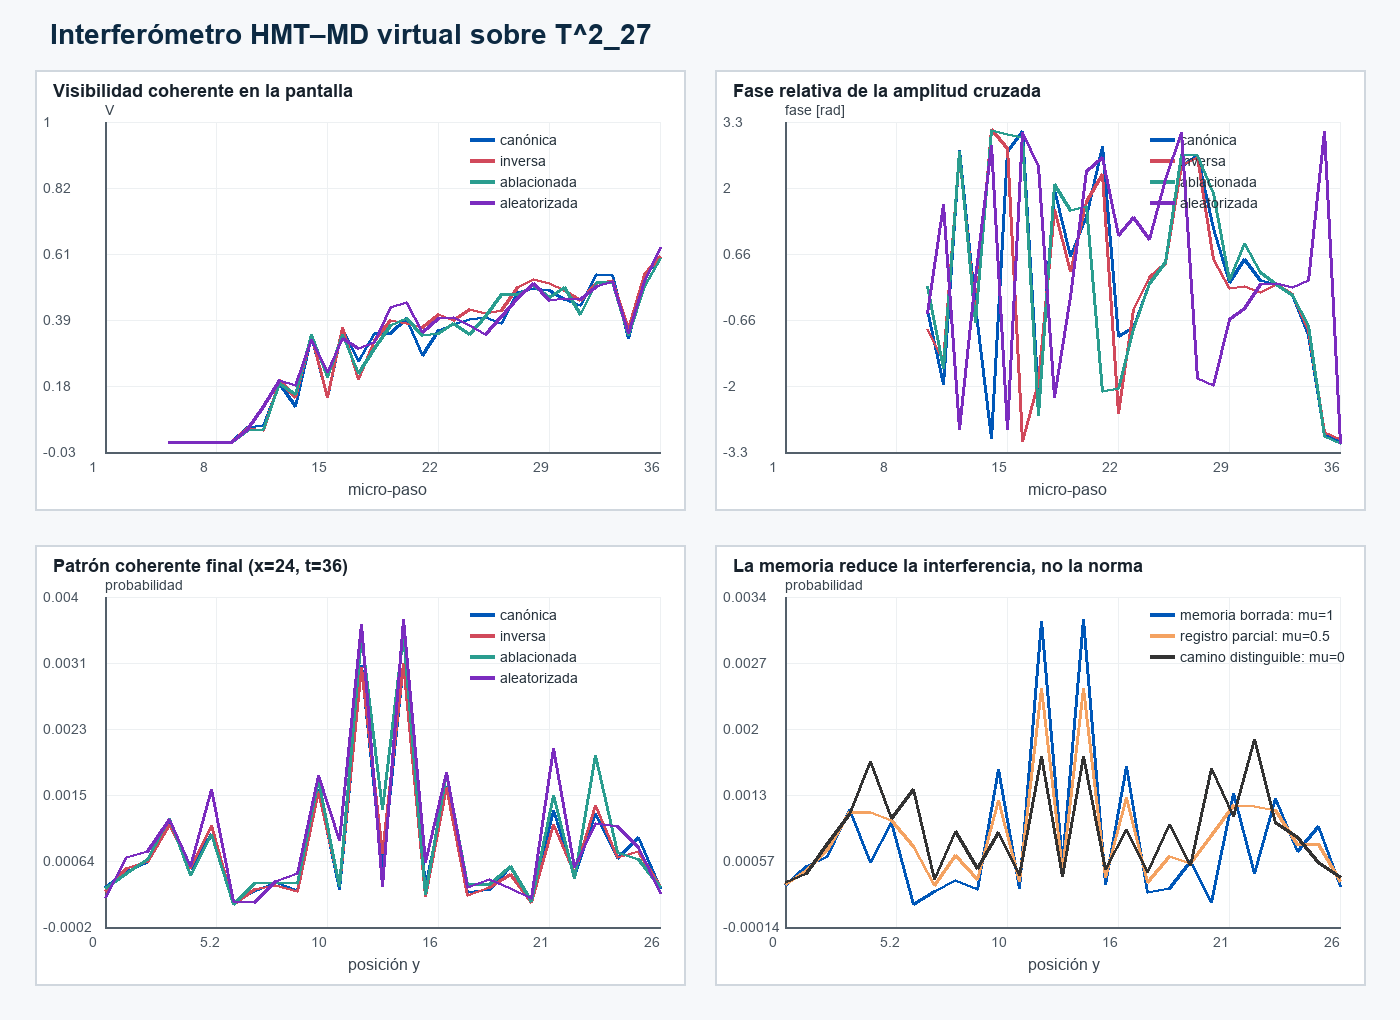
\includegraphics[width=.96\linewidth]{figures/parte_iv/01_curvas_y_patrones.png}
\caption{Evolución de la visibilidad, fase relativa y patrón final para las cuatro secuencias con presupuesto común.}
\label{fig:md-sucesora-interferometro-patrones}
\end{figure}

\begin{figure}[tbp]
\centering
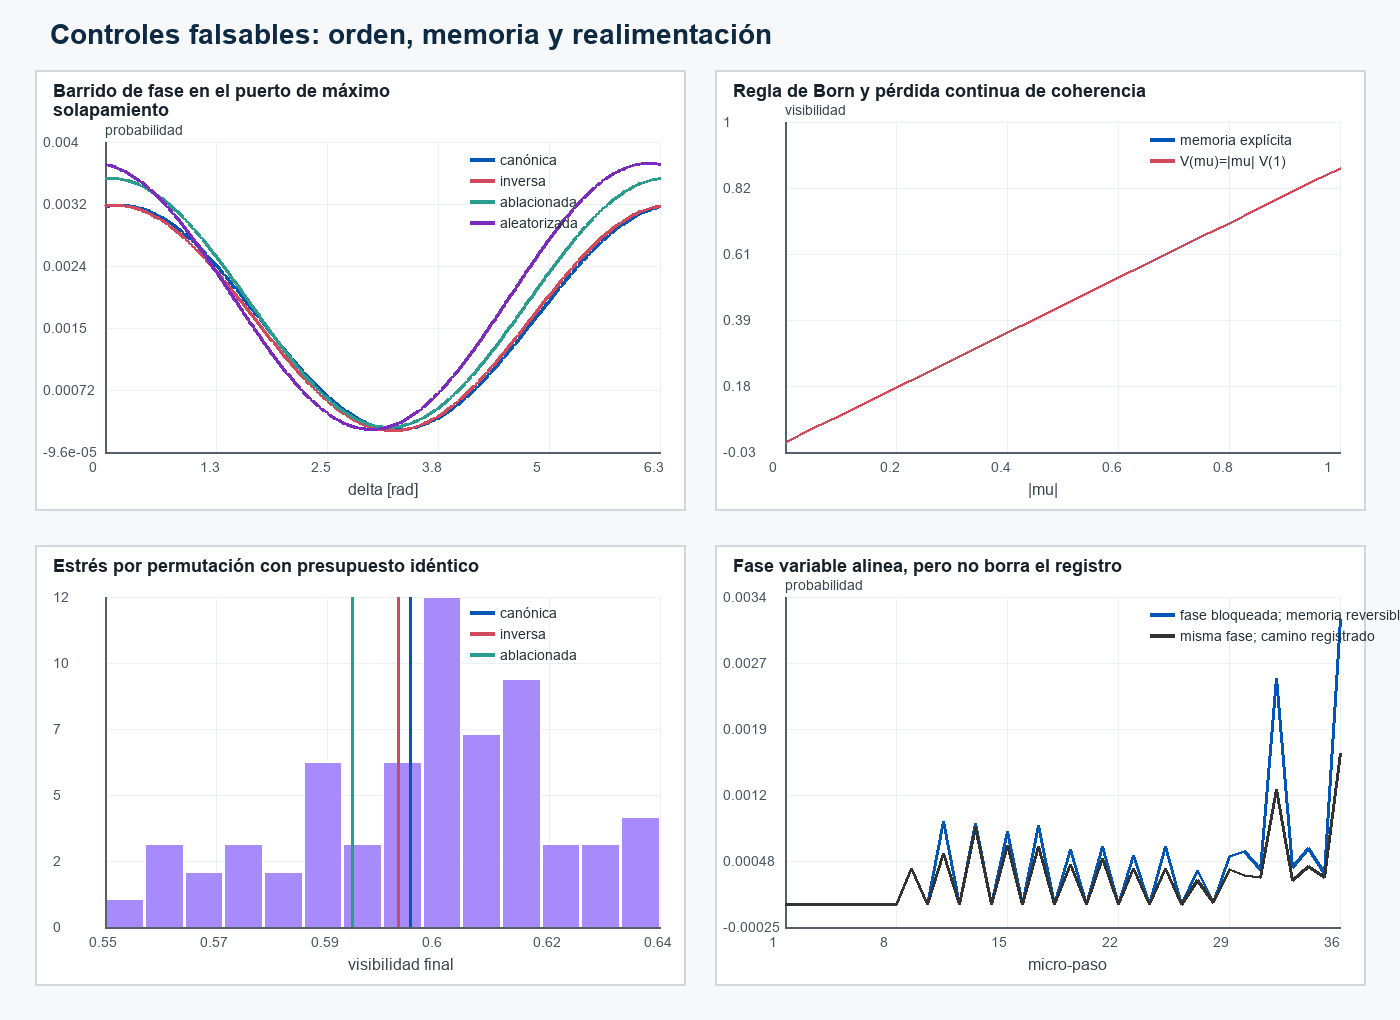
\includegraphics[width=.96\linewidth]{figures/parte_iv/02_estres_memoria_y_control.png}
\caption{Controles de orden, memoria de camino y realimentación de fase.}
\label{fig:md-sucesora-interferometro-controles}
\end{figure}

\endgroup

\begingroup
\def\HMTDesiredChapterTitle{Estadísticas cuánticas de ocupación: distribuciones de Fermi--Dirac y Bose--Einstein}%
\let\HMTOriginalChapter\chapter
\renewcommand{\chapter}[2][]{\HMTOriginalChapter{\HMTDesiredChapterTitle}}%
\chapter{Estadísticas cuánticas de ocupación: distribuciones de Fermi–Dirac y Bose–Einstein}
\label{chap:parte-iv-55}

La enumeración microcanónica y las completaciones simétrica y antisimétrica producen las leyes de Bose--Einstein y Fermi--Dirac. El límite de Maxwell--Boltzmann se mantiene como régimen derivado, no como punto de partida.

\section{Enumeración microcanónica de estados sobre una pantalla finita}

Consideremos la realización finita
\[
 \mathcal H_{\rm occ}=\bigoplus_{k=0}^{3}\CC^{g_k},
 \qquad
 H_{\rm occ}|_{\CC^{g_k}}=E_k^{\rm occ} I,
\]
con niveles y multiplicidades
\[
 E^{\rm occ}=(0,3,6,9),\qquad g=(1,6,12,8),
 \qquad(N,E)=(12,66).
\]
La suma \(1+6+12+8=27\) hace de \(\mathcal H_{\rm occ}\) una pantalla de
veintisiete modos. Este espectro es el dato de una representación finita
declarada; su cardinal no basta para identificarla con cualquier otra
aparición de \(27\) en HMT\@. El morfismo que relaciona una pantalla concreta
de frontera con \((\mathcal H_{\rm occ},H_{\rm occ})\) debe especificar tanto
las fibras como el operador espectral.
Las funciones generadoras fermiónica y bosónica son
\[
 F(y,x)=\prod_k(1+yx^{E_k^{\rm occ}})^{g_k},
 \qquad
 B(y,x)=\prod_k(1-yx^{E_k^{\rm occ}})^{-g_k}.
\]

\begin{proposition}[Cardinalidades microcanónicas]
\label{prop:cardinalidades-microcanonicas}
\[
 [y^{12}x^{66}]F=2\,104\,494,
 \qquad
 [y^{12}x^{66}]B=259\,436\,430.
\]
\end{proposition}
\begin{proof}
En el producto fermiónico, elegir \(r\) de los \(g_k\) modos contribuye
\(\binom{g_k}{r}y^rx^{rE_k^{\rm occ}}\). En el bosónico, distribuir \(r\)
ocupaciones indistinguibles entre \(g_k\) modos contribuye
\(\binom{g_k+r-1}{r}y^rx^{rE_k^{\rm occ}}\). La convolución finita sobre los
cuatro niveles produce los enteros indicados.
\end{proof}

\section{Distribuciones de Bose--Einstein y Fermi--Dirac}

La formulación de equilibrio parte del Hamiltoniano y del número total de
ocupaciones,
\begin{equation}
 H=\sum_kE_k^{\rm occ} n_k,
 \qquad
 N=\sum_k n_k,
 \qquad
 K_\mu:=H-\mu N.
 \label{eq:hamiltoniano-gran-canonico-rev3}
\end{equation}
Para \(\beta>0\), el estado gran canónico es
\begin{equation}
 \rho_{\beta,\mu}
 =\frac{e^{-\beta K_\mu}}{\mathcal Z_{\beta,\mu}},
 \qquad
 \mathcal Z_{\beta,\mu}
 =\operatorname{Tr}(e^{-\beta K_\mu}).
 \label{eq:estado-gran-canonico-rev3}
\end{equation}

\begin{theorem}[Factorización gran canónica y leyes de ocupación]
\label{thm:factorizacion-gran-canonica-rev3}
Para niveles de energía \(E_k^{\rm occ}\) con degeneraciones \(g_k\), la
traza fermiónica factoriza como
\begin{equation}
 \mathcal Z_{\rm FD}
 =\prod_k\bigl(1+e^{-\beta(E_k^{\rm occ}-\mu)}\bigr)^{g_k},
 \qquad
 \langle n_k\rangle_{\rm FD}
 =\frac{g_k}{e^{\beta(E_k^{\rm occ}-\mu)}+1}.
 \label{eq:factorizacion-fd-rev3}
\end{equation}
En el sector bosónico, bajo la condición
\(\mu<\inf_kE_k^{\rm occ}\),
\begin{equation}
 \mathcal Z_{\rm BE}
 =\prod_k\bigl(1-e^{-\beta(E_k^{\rm occ}-\mu)}\bigr)^{-g_k},
 \qquad
 \langle n_k\rangle_{\rm BE}
 =\frac{g_k}{e^{\beta(E_k^{\rm occ}-\mu)}-1}.
 \label{eq:factorizacion-be-rev3}
\end{equation}
\end{theorem}

\begin{proof}
El operador \(K_\mu\) es una suma de operadores de ocupación conmutantes, de
modo que su traza factoriza por modos. En cada modo fermiónico se suman las
ocupaciones \(0\) y \(1\), y el factor correspondiente es
\(1+u_k\), donde
\(u_k=e^{-\beta(E_k^{\rm occ}-\mu)}\). En cada modo bosónico se suman todas
las ocupaciones no negativas y se obtiene la serie geométrica
\((1-u_k)^{-1}\); la condición sobre \(\mu\) garantiza \(u_k<1\). Las
potencias \(g_k\) incorporan la degeneración. Finalmente,
\[
 \langle n_k\rangle
 =-\frac1\beta\frac{\partial}{\partial E_k^{\rm occ}}
   \log\mathcal Z
\]
produce las dos leyes de ocupación
\cite{Bose1924,Einstein1924,Fermi1926,Dirac1926,Pathria2011}.
\end{proof}

La derivación microcanónica recupera el mismo resultado en el régimen
termodinámico. Para ocupaciones fermiónicas medias
\(p_k=m_k/g_k\), la entropía combinatoria por nivel es
\begin{equation}
 S_k\simeq
 g_k\bigl[-p_k\log p_k-(1-p_k)\log(1-p_k)\bigr].
 \label{eq:entropia-fd-nivel-rev3}
\end{equation}
La variación de \(\sum_kS_k\), sujeta a
\(\sum_kg_kp_k=N\) y
\(\sum_kg_kE_k^{\rm occ}p_k=E\), da
\begin{equation}
 \log\frac{1-p_k}{p_k}=\alpha+\beta E_k^{\rm occ},
 \qquad
 \mu=-\frac{\alpha}{\beta},
 \label{eq:variacion-fd-rev3}
\end{equation}
y, por tanto, la ocupación de Fermi--Dirac de
\eqref{eq:factorizacion-fd-rev3}. Los multiplicadores \(\beta\) y \(\mu\)
son las coordenadas duales de las restricciones de energía y población.

Para ocupaciones bosónicas medias
\(\overline n_k=m_k/g_k\), la logmultiplicidad del nivel es
\begin{equation}
 S_k\simeq
 g_k\bigl[(1+\overline n_k)\log(1+\overline n_k)
          -\overline n_k\log\overline n_k\bigr].
 \label{eq:entropia-be-nivel-rev3}
\end{equation}
La variación de \(\sum_kS_k\), sujeta a
\(\sum_kg_k\overline n_k=N\) y
\(\sum_kg_kE_k^{\rm occ}\overline n_k=E\), produce
\begin{equation}
 \log\frac{1+\overline n_k}{\overline n_k}
 =\alpha+\beta E_k^{\rm occ},
 \qquad
 \overline n_k
 =\frac{1}{e^{\beta(E_k^{\rm occ}-\mu)}-1},
 \qquad
 \mu=-\frac{\alpha}{\beta}.
 \label{eq:variacion-be-rev3}
\end{equation}
Ésta es la ocupación de Bose--Einstein de
\eqref{eq:factorizacion-be-rev3}. La condición
\(\mu<\inf_kE_k^{\rm occ}\) asegura la positividad del denominador y la
convergencia de cada factor modal.

En la instancia finita construida, las dos restricciones determinan
\[
 (\beta_{\rm FD},\mu_{\rm FD})
 =(0.15307011353415928,\,4.502865197597043),
\]
\[
 (\beta_{\rm BE},\mu_{\rm BE})
 =(0.05456727960068316,\,-15.92569781906737).
\]
Si \(m_k^{\rm mic}\) denota la ocupación media obtenida por enumeración
microcanónica exacta y \(m_k^{\rm eq}\) la evaluación de la distribución
correspondiente, los errores
\(\sum_k|m_k^{\rm mic}-m_k^{\rm eq}|\) son
\[
 0.09897380039002812\quad\hbox{y}\quad
 0.9190625715582017,
\]
respectivamente. La enumeración recorre todas las cuádruplas de ocupación,
calcula sus multiplicidades enteras y resuelve las dos ecuaciones de
restricción. Las dos leyes se realizan sobre una misma pantalla. La elección
física entre ellas exige una graduación y un Hamiltoniano compatibles con la
representación de la trayectoria. El parámetro térmico se tipará más adelante
como \(\beta=(k_B\Theta)^{-1}\).

\section{Convergencia cuantificada hacia la distribución de Maxwell--Boltzmann}

La relación entre las dos estadísticas cuánticas y el régimen clásico puede
formularse sin recurrir a una aproximación informal. Para cada modo, sea
\[
 u_k:=e^{-\beta(E_k^{\rm occ}-\mu)}.
\]
Las ocupaciones por estado se escriben
\[
 \overline n_k^{\rm FD}=\frac{u_k}{1+u_k},
 \qquad
 \overline n_k^{\rm BE}=\frac{u_k}{1-u_k};
\]
las multiplicidades \(g_k\) se incorporan después mediante
\(\langle n_k\rangle=g_k\overline n_k\).

\begin{theorem}[Límite clásico común de las estadísticas cuánticas]
\label{thm:limite-clasico-fd-be-rev2}
Si \(0\leq u_k\leq\delta<1\), entonces
\[
 \left|\overline n_k^{\rm FD}-u_k\right|\leq u_k^2,
 \qquad
 \left|\overline n_k^{\rm BE}-u_k\right|
 \leq\frac{u_k^2}{1-\delta}.
\]
En consecuencia, en el régimen diluido \(u_k\to0\),
\[
 \boxed{
 \overline n_k^{\rm FD}\sim
 \overline n_k^{\rm BE}\sim
 e^{-\beta(E_k^{\rm occ}-\mu)}} ,
\]
que es la distribución de Maxwell--Boltzmann por modo.
\end{theorem}

\begin{proof}
Las identidades exactas
\[
 u_k-\frac{u_k}{1+u_k}=\frac{u_k^2}{1+u_k},
 \qquad
 \frac{u_k}{1-u_k}-u_k=\frac{u_k^2}{1-u_k}
\]
proporcionan las cotas. Para \(0<u_k\leq\delta\), al dividir por \(u_k\) y
tomar \(u_k\downarrow0\) se obtiene
la equivalencia asintótica. El primer término de orden \(u_k^2\) conserva la
diferencia física: la exclusión disminuye la ocupación fermiónica, mientras
la acumulación aumenta la ocupación bosónica.
\end{proof}


\section{Completaciones cuánticas, holonomía de hoja y periodicidad estadística}

Las completaciones simétrica y exterior, la graduación de hoja, la holonomía
\(2\pi/4\pi\), los conteos de ocupación y el complejo celular de APP forman un
único antecedente algebraico de las estadísticas cuánticas. Se incorpora aquí
el desarrollo íntegro para que la periodicidad no quede reducida a una mera
referencia posterior.

\begingroup
\let\chapter\section
\let\section\subsection
\let\subsection\subsubsection
\let\subsubsection\paragraph
\let\clearpage\relax
\let\cleardoublepage\relax
\chapter{Completaciones estadísticas y campos sobre APP}
\label{chap:completaciones-cuanticas}

Las palabras Bose, Fermi, Pauli o fotón no designan por sí solas teoremas de
un sistema discreto. Para obtenerlos hay que especificar un espacio de estados,
una graduación, un producto y operadores. APP y TPK proporcionan un conjunto
de estados orientados y una paridad de hoja. A partir de esos datos pueden
construirse dos completaciones universales: el álgebra simétrica y el álgebra
exterior. Esta sección identifica exactamente lo que se sigue de la
construcción y separa la estadística algebraica de su interpretación física.

\section{Espacio lineal de estados asociado a una realización de partícula}

Sea \(S\) un conjunto finito de clases de rutas TPK a la profundidad elegida
y sea
\[
 \mathcal H_1=\ell^2(S)
\]
el espacio de Hilbert con base ortonormal \((e_s)_{s\in S}\). Una elección de
pesos positivos \(E_s\) define el operador diagonal
\[
 He_s=E_se_s.
\]
La elección de \(S\), de su cociente por simetrías y de los pesos forma parte
del modelo. Una vez fijada, las completaciones multipartícula son canónicas.

\section{Completaciones simétrica y exterior}

Definimos
\[
 \mathcal F_+(\mathcal H_1)=
 \bigoplus_{n\geq0}\operatorname{Sym}^n\mathcal H_1,
 \qquad
 \mathcal F_-(\mathcal H_1)=
 \bigoplus_{n\geq0}\bigwedge^n\mathcal H_1.
\]
La primera es la completación bosónica; la segunda, la fermiónica.

\begin{theorem}[Principio de exclusión de Pauli en la completación exterior]
Para todo modo \(s\in S\), los operadores de creación y aniquilación de la
completación exterior satisfacen
\[
 \{a_s,a_t^\dagger\}=\delta_{st}I,
 \qquad
 \{a_s,a_t\}=\{a_s^\dagger,a_t^\dagger\}=0.
\]
En particular, el operador de ocupación
\(N_s=a_s^\dagger a_s\) es un proyector:
\[
 N_s^2=N_s,
\]
y sus autovalores son \(0,1\).
\end{theorem}

\begin{proof}
La creación es el producto exterior por \(e_s\); la aniquilación es su
adjunto. La antisimetría implica \(e_s\wedge e_s=0\) y da las relaciones
canónicas por cálculo sobre la base exterior. Entonces
\[
N_s^2=a_s^\dagger a_sa_s^\dagger a_s
=a_s^\dagger(I-a_s^\dagger a_s)a_s=N_s.
\]
Todo proyector autoadjunto posee espectro contenido en \(\{0,1\}\).
\end{proof}

El principio de exclusión aparece así como teorema de la completación
exterior. La cuestión específicamente HMT es qué dato del transporte elige
esa completación para una clase de rutas.

\section{Graduación de hoja y álgebra de intercambio}

Supongamos que la hoja orientada define un carácter aditivo
\[
 p:\operatorname{Mor}(\mathsf P_{\rm TPK})\longrightarrow\mathbb Z/2\mathbb Z,
 \qquad p(\gamma\eta)=p(\gamma)+p(\eta).
\]
Sobre el espacio lineal graduado correspondiente se introduce la simetría
\[
 \tau(v\otimes w)=(-1)^{p(v)p(w)}w\otimes v.
\]

\begin{theorem}[Completación estadística determinada por la paridad]
El cociente del álgebra tensorial por las relaciones
\[
 v\otimes w-(-1)^{p(v)p(w)}w\otimes v
\]
es simétrico sobre el sector par y exterior sobre el sector impar. Dos estados
impares idénticos tienen producto nulo; los estados pares admiten ocupación
arbitraria.
\end{theorem}

\begin{proof}
Si \(p(v)=p(w)=0\), la relación es \(vw=wv\). Si
\(p(v)=p(w)=1\), es \(vw=-wv\); tomando \(v=w\) y trabajando en
característica cero se obtiene \(v^2=0\). Los sectores mixtos conmutan sin
signo adicional. Esta es la propiedad universal del álgebra simétrica
graduada.
\end{proof}

El teorema convierte una paridad composicional TPK en una regla exacta de
ocupación. Para obtener el teorema físico de espín--estadística hay que
construir además una teoría local lorentziana positiva y demostrar que la
paridad de hoja coincide con el espín bajo rotaciones. La igualdad no se
deduce únicamente de que ambos objetos tomen valores módulo dos.

\section{Holonomía de hoja y periodicidad de \texorpdfstring{\(2\pi/4\pi\)}{2pi/4pi}}

La paridad anterior admite una realización geométrica natural cuando una
extensión superviviente posee un retorno cerrado cuya cubierta de orientación
es no trivial. Sea \(\rho\) el generador del retorno y sea
\[
 \varepsilon:\langle\rho\rangle\longrightarrow\{-1,+1\}
\]
su carácter de holonomía, con \(\varepsilon(\rho)=-1\). El fibrado real
asociado es entonces la línea de orientación de una banda de Möbius: una
vuelta cierra la proyección geométrica, pero cambia la hoja levantada; dos
vueltas restauran la orientación.

Para escribir esta propiedad angularmente, fijemos una representación
unitaria \(U\) de la cubierta de rotaciones sobre el espacio graduado
\(\mathcal H_1=\mathcal H_{\bar0}\oplus\mathcal H_{\bar1}\), compatible con
la paridad de hoja en el sentido
\[
 U(2\pi)v=(-1)^{p(v)}v
\]
para todo vector homogéneo \(v\). La compatibilidad es una condición de la
realización: identifica el generador de la cubierta de orientación con el
carácter \(p\) ya construido sobre las rutas.

\begin{theorem}[Restauración de orientación y álgebra de intercambio]
\label{thm:dos-cuatro-pi-estadistica}
Bajo la compatibilidad precedente,
\[
 U(2\pi)|_{\mathcal H_{\bar0}}=I,
 \qquad
 U(2\pi)|_{\mathcal H_{\bar1}}=-I,
 \qquad
 U(4\pi)=I.
\]
Además, el mismo carácter \(p\) determina la simetría graduada
\[
 \tau(v\otimes w)=(-1)^{p(v)p(w)}w\otimes v.
\]
Por tanto, el sector de holonomía par se completa mediante potencias
simétricas y el sector de holonomía impar mediante potencias exteriores. En
el segundo se cumple la exclusión \(v\wedge v=0\).
\end{theorem}

\begin{proof}
La primera y la segunda igualdad son la condición de compatibilidad evaluada
en cada componente homogénea. Al iterar una vuelta,
\[
 U(4\pi)v=U(2\pi)^2v=(-1)^{2p(v)}v=v,
\]
lo que demuestra la restauración. La afirmación sobre el intercambio es el
teorema de completación por paridad de la sección anterior: para dos vectores
pares el signo es positivo, mientras que para dos impares es negativo.
\end{proof}

Conviene distinguir tres retornos. El cierre angular tras \(2\pi\) es un
retorno de la proyección; el cierre tras \(4\pi\) restaura la orientación
levantada; ninguno obliga por sí solo a que todas las coordenadas del registro
regresen a su valor inicial. Esta separación es la análoga dimensional de la
distinción HMT entre retorno de fase y retorno de estado.

\subsection{Las hojas suma y producto como soportes de las \(2\) completaciones}

La tabla APP contiene dos evaluaciones sobre un mismo soporte. La hoja
aditiva actúa por traslaciones y conserva la multiplicidad de las
continuaciones; en este sentido, acumula. La hoja multiplicativa es
permutativa sobre las unidades y contrae fibras sobre los no invertibles; en
este sentido, pliega. Esta incompatibilidad es anterior a la elección
estadística y explica por qué TPK debe conservar dos genealogías en lugar de
reducirlas a una sola palabra visible.

La asignación estadística no se obtiene, sin embargo, sustituyendo
verbalmente «suma» por «bosón» y «producto» por «fermión». El mapa exacto es
el carácter de paridad
\[
 p:\operatorname{Mor}(\mathsf P_{\rm TPK})\longrightarrow\mathbb Z/2\mathbb Z.
\]
Cuando el transporte de una extensión cae en el sector \(p=0\), su
completación admite ocupación acumulativa y es simétrica. Cuando cae en
\(p=1\), la reversión de hoja introduce el signo de intercambio y la
completación es exterior. La suma y el producto suministran las dos
geometrías locales; el registro, la orientación y el carácter \(p\) deciden en
qué sector se realiza una ruta.

Con un Hamiltoniano diagonal \(H\), energía \(\epsilon\), potencial químico
\(\mu\) y parámetro térmico \(\beta\), las ocupaciones medias de los dos
sectores son entonces
\[
 \bar n_{\rm par}(\epsilon)
 =\frac{1}{e^{\beta(\epsilon-\mu)}-1},
 \qquad
 \bar n_{\rm impar}(\epsilon)
 =\frac{1}{e^{\beta(\epsilon-\mu)}+1}.
\]
Las fórmulas de Bose--Einstein y Fermi--Dirac son, por tanto, las
evaluaciones termodinámicas de las completaciones simétrica y exterior
seleccionadas por el transporte. La periodicidad \(4\pi\) y la exclusión
fermiónica quedan coordinadas por el mismo carácter, pero ninguna de las dos
se infiere de una mera coincidencia numérica.

\section{Operadores de número y distribución de ocupación en la realización de Fock}

Si hay \(g\) modos y \(N\) partículas, las dimensiones de los sectores son
\[
 \Omega_F(g,N)=\binom gN,
 \qquad
 \Omega_B(g,N)=\binom{g+N-1}{N}.
\]
La primera fórmula cuenta subconjuntos de modos; la segunda, composiciones
débiles de \(N\) en \(g\) partes. Estos conteos son consecuencias exactas de
las dos completaciones y no requieren una hipótesis termodinámica.

\section{El complejo celular del toro APP}

El grafo de APP es el uno-esqueleto de una descomposición celular del toro
\(T^2\) con \(9\times9\) vértices. Sea
\[
 C^0\xrightarrow{d_0}C^1\xrightarrow{d_1}C^2
\]
su complejo de cocadenas reales. Elegido el producto escalar uniforme,
definimos la codiferencial \(\delta=d^*\) y el laplaciano
\[
 \Delta_k=d_{k-1}\delta_k+\delta_{k+1}d_k.
\]

\begin{theorem}[Sector armónico del toro digital]
La dimensión del espacio de uno-formas armónicas es dos:
\[
 \dim\ker\Delta_1=b_1(T^2)=2.
\]
Puede elegirse una base representada por los flujos uniformes horizontal y
vertical. Ambos son cerrados, cocerrados y no son gradientes de funciones
globales periódicas.
\end{theorem}

\begin{proof}
El teorema de Hodge para complejos celulares finitos identifica
\(\ker\Delta_1\) con \(H^1(T^2;\mathbb R)\). La cohomología del toro tiene
rango dos. Directamente, los flujos constantes horizontal y vertical tienen
divergencia y rotacional nulos; sus integrales sobre los dos ciclos
fundamentales son independientes, por lo que no son exactos.
\end{proof}

El espacio de conexiones módulo transformaciones de calibre es
\[
 C^1/\operatorname{im}d_0.
\]
En un complejo finito provisto del producto escalar anterior, cada órbita
admite un representante de Coulomb en \(\ker\delta_1\); dentro de la órbita,
la elección es única módulo el estabilizador \(\ker d_0\) del parámetro de
calibre. El cociente cohomológico correcto es
\[
 \ker d_1/\operatorname{im}d_0
 \simeq \ker\Delta_1 .
\]
Sus dos clases armónicas constituyen un candidato matemático natural para
dos modos globales libres. No son todavía las dos polarizaciones locales de
un fotón en espacio-tiempo \(3+1\): para esa identificación se necesita un
límite dinámico, una relación de dispersión y un grupo físico de calibre.

\section{Ley de Gauss discreta}

Para una 1-cocadena orientada \(F\) y un conjunto de vértices \(V\), la
divergencia se define por
\[
 (\operatorname{div}F)(v)=
 \sum_{e:v\to w}F(e)-\sum_{e:w\to v}F(e).
\]
Al sumar sobre \(V\), toda arista interior aparece una vez con cada signo y
se cancela. Por tanto,
\[
 \boxed{
 \sum_{v\in V}\operatorname{div}F(v)
 =\operatorname{Flux}_{\partial V}(F).}
\]
Esta identidad es una ley de Gauss exacta en el grafo. Interpretar
\(\operatorname{div}F\) como carga eléctrica exige el carácter de carga y la
realización dimensional construidos en Mecánica Dimensional.

\section{Aparato de medición reversible}

Sea \(S\) un conjunto de estados y sea \(r:S\to\mathbb Z/9\mathbb Z\) una
lectura. El acoplamiento a un registro nonádico se define por
\[
 U_r:S\times\mathbb Z/9\mathbb Z\longrightarrow
 S\times\mathbb Z/9\mathbb Z,
 \qquad
 U_r(s,a)=(s,a+r(s)).
\]

\begin{proposition}[Reversibilidad del acoplamiento]
La aplicación \(U_r\) es una permutación y
\[
 U_r^{-1}(s,a)=(s,a-r(s)).
\]
La pérdida de información sólo aparece después de aplicar un lector al
registro o de condicionar el estado por el resultado.
\end{proposition}

\begin{proof}
La fórmula propuesta para la inversa satisface ambas composiciones por la
ley de grupo de \(\mathbb Z/9\mathbb Z\).
\end{proof}

Esta proposición formaliza la definición operativa de medición: acoplar,
leer y restringir futuros compatibles son tres aplicaciones diferentes. El
acoplamiento completo es reversible; el cociente observacional puede no serlo.

\section{Correspondencias algebraicas y realizaciones físicas}

Las completaciones de Fock, la exclusión condicionada a paridad, el sector
armónico de APP, Gauss discreto y la reversibilidad del aparato son teoremas
matemáticos completos. Sus identificaciones físicas forman un diagrama que
debe conmutar:
\[
 \text{paridad de hoja}
 \longrightarrow\text{intercambio graduado}
 \longrightarrow\text{CAR/CCR}
 \longrightarrow\text{estadística física},
\]
\[
 H^1(\mathcal A_9)
 \longrightarrow\text{campo discreto de calibre}
 \longrightarrow\text{modo sin masa}
 \longrightarrow\text{fotón}.
\]
Las dos primeras flechas de cada línea poseen construcciones explícitas; las
últimas requieren la dinámica y el límite físico correspondientes. Esta
separación permite desarrollar los puentes sin confundir una analogía de
cardinalidad con una representación.

\endgroup

\paragraph{De la medición reversible a la ocupación fermiónica y al principio algebraico de exclusión de Pauli} La distinción estadística se completa algebraicamente mediante la idempotencia de ocupación y la exclusión fermiónica.

\endgroup
% Contenido exclusivo del propietario de entropías tipadas.
\subsection{Correlación cuasilibre y entropías espectrales de ocupación}

Para un estado fermiónico cuasilibre gauge-invariante, conservador del
número y definido sobre un espacio de un cuerpo de dimensión finita, sea
\(C_{ij}=\langle a_j^\dagger a_i\rangle\) el operador de correlación de un
cuerpo. La hipótesis gauge-invariante excluye correlaciones anómalas de
emparejamiento, de modo que \(C\) determina el estado cuasilibre. Si
\(0<C<I\), su generador modular de un cuerpo y la reconstrucción recíproca
del correlador son
\begin{equation}
 \boxed{
 K_1=\log\bigl((I-C)C^{-1}\bigr),
 \qquad
 C=(I+e^{K_1})^{-1}.}
 \label{eq:puente-cuasilibre-modular-rev3}
\end{equation}

\begin{corollary}[Forma logística del espectro modular]
\label{cor:forma-logistica-modular-rev3}
Si \(K_1u_i=\kappa_i u_i\), la ocupación del modo \(u_i\) es
\[
 \langle n_i\rangle=\frac1{1+e^{\kappa_i}}.
\]
Para \(\kappa_i=\beta(\varepsilon_i-\mu)\), se recupera la ley de
Fermi--Dirac.
\end{corollary}

\begin{proof}
La diagonalización espectral de \(K_1\) diagonaliza toda función suya. La
aplicación de \(x\mapsto(1+e^x)^{-1}\) a cada autovalor produce la fórmula.
\end{proof}

Si \(C\) tiene autovalores \(p_i\in[0,1]\), la entropía de ocupación del
estado fermiónico cuasilibre es, con la convención \(0\log0=0\),
\begin{equation}
 S_F=-\sum_i\bigl[p_i\log p_i+(1-p_i)\log(1-p_i)\bigr].
 \label{eq:entropia-cuasilibre-fermi-rev3}
\end{equation}
Para un estado bosónico gaussiano diagonal con un número finito de modos y
ocupaciones medias \(\overline n_i\),
\begin{equation}
 S_B=\sum_i\bigl[(1+\overline n_i)\log(1+\overline n_i)
                  -\overline n_i\log\overline n_i\bigr].
 \label{eq:entropia-gaussiana-bose-rev3}
\end{equation}
La misma fórmula se extiende a una familia numerable cuando la serie del
miembro derecho converge.
Estas entropías cuantifican configuraciones de ocupación. La entropía de
entrelazamiento posee otro dominio: el estado reducido inducido por una
descomposición tensorial. La identificación entre ambas requiere declarar la
reducción y el operador de correlación que la implementan.

Finalmente, para un estado reducido \(\rho_A\), la \emph{entropía de von
Neumann}
\[
 S_{\rm vN}(\rho_A)=-\operatorname{Tr}(\rho_A\log\rho_A)
\]
es una propiedad espectral del operador de densidad. Cuando \(\rho_A\)
procede de una purificación global, cuantifica el entrelazamiento a través
del corte. En la construcción de borde HMT, el operador de área, el
Hamiltoniano modular y la reducción correspondiente permanecen en la
\cref{hap:sec:area-entrelazamiento-barbero-rev11}.

Los mapas entre estos dominios se publican mediante identidades explícitas.
La descomposición de una medida por las fibras de \(q\) satisface la regla de
la cadena
\begin{equation}
 \mathsf H_\mu(\mathbf X)
 =\mathsf H_{q_*\mu}(q(\mathbf X))
  +\mathsf H_{\rm fib}(q;\mu).
 \label{eq:cadena-entropia-fibras-rev2}
\end{equation}
\Needspace{5\baselineskip}
Una distribución finita \(p=(p_i)\) se realiza diagonalmente como
\[
 \rho_p=\sum_i p_i|i\rangle\langle i|,
 \qquad S_{\rm vN}(\rho_p)=\mathsf H(p).
\]
Si \(P_{N,E}\) proyecta sobre el subespacio microcanónico de dimensión
\(\Omega(N,E)\), entonces
\[
 \rho_{\rm mc}=\frac{P_{N,E}}{\Omega(N,E)},
 \qquad S_{\rm vN}(\rho_{\rm mc})=\log\Omega(N,E)=S_{\rm mc}.
\]
Para un estado puro bipartito,
\[
 \rho_A=\operatorname{Tr}_B
 \bigl(|\Psi_{AB}\rangle\langle\Psi_{AB}|\bigr)
\]
define la reducción que mide el entrelazamiento. Finalmente, la igualdad entre
\(h_{\rm top}=\log\rho(A)\) y una entropía métrica se alcanza, para este
sistema primitivo, mediante la medida de Parry, que realiza la entropía métrica
máxima; no se atribuye a una medida arbitraria de historias.



\begingroup
\def\HMTDesiredChapterTitle{Completación fermiónica de las trayectorias y principio algebraico de exclusión de Pauli}%
\let\HMTOriginalChapter\chapter
\renewcommand{\chapter}[2][]{\HMTOriginalChapter{\HMTDesiredChapterTitle}}%
\chapter{Completación fermiónica de las trayectorias y principio algebraico de exclusión de Pauli}
\label{chap:parte-iv-56}

La completación exterior de las trayectorias impone idempotencia y exclusión antes de cualquier identificación de especie. Los caracteres de giro, color, sabor y virtualidad conservan su tipado dentro de la representación correspondiente.

\section{Ocupación, exclusión y estadística finita}
\label{chap:ocupacion-estadistica}
\index{Pauli, principio de exclusión de}\index{CAR}
\index{Fermi--Dirac}\index{Bose--Einstein}

Las realizaciones nula y material proporcionan el soporte geométrico de la
ocupación. El sector fermiónico se construye sobre las relaciones canónicas de
anticonmutación (CAR), y el teorema de espín--estadística exige además la
representación operatoria declarada. Esta sección fija esas premisas antes de
derivar la idempotencia de la ocupación, las cardinalidades microcanónicas y
las distribuciones de Bose--Einstein y Fermi--Dirac con su límite clásico
común.

\subsection{Idempotencia de la ocupación en el álgebra de anticonmutación}

Sean \(a_i,a_i^\dagger\) operadores que satisfacen las relaciones canónicas
de anticonmutación (CAR)
\[
 \{a_i,a_j^\dagger\}=\delta_{ij},
 \qquad \{a_i,a_j\}=0,
\]
y sea \(n_i=a_i^\dagger a_i\).

\begin{theorem}[Principio de exclusión de Pauli]
\label{thm:principio-exclusion-pauli}
Se cumple \(n_i^2=n_i\), y por tanto
\(\Spec(n_i)\subseteq\{0,1\}\).
\end{theorem}
\begin{proof}
\[
 n_i^2=a_i^\dagger a_i a_i^\dagger a_i
 =a_i^\dagger(1-a_i^\dagger a_i)a_i
 =a_i^\dagger a_i,
\]
porque \(a_i^2=(a_i^\dagger)^2=0\). Todo autovalor de un idempotente
satisface \(\lambda^2=\lambda\) \cite{Pauli1925,Dirac1926}.
\end{proof}

La nilpotencia \((a_i^\dagger)^2=0\) impide la ocupación fermiónica doble del
mismo modo y conduce, al maximizar la entropía bajo las restricciones de
energía y número, a la ley de ocupación de Fermi--Dirac expuesta más adelante.
La completación simétrica y la ley de Bose--Einstein constituyen un estrato
distinto y se presentan por separado.

Las relaciones CAR son una hipótesis algebraica del teorema. Una monodromía
con cambio de signo bajo una rotación de \(2\pi\) es compatible con una
representación fermiónica, pero no constituye por sí sola una derivación de
CAR ni del teorema espín--estadística.


\section{Caracteres de giro, color, sabor y virtualidad}

Sea \(\jmath:\Gamma_{\rm TPK}\to\Gamma_{\rm TPK}\) la involución que invierte
la orientación de cada arista y permuta las fibras mediante
\(J_c:E_c\to E_{\jmath c}\). Un carácter de giro es una representación
\(\rho_{\rm rot}\) del subgrupo generado por \(\jmath\) sobre las secciones;
sus autoespacios de signos \(+1\) y \(-1\) son objetos algebraicos distintos
de una representación física del grupo de Lorentz.

Sea \(\mathcal C\) el grupo abeliano de caracteres de canal del transporte.
Dos secciones poseen el mismo \emph{sabor aritmético} cuando sus caracteres
\[
 \chi_s:\mathcal C\longrightarrow\CC^\times
\]
coinciden. La identificación de estas clases con sabores de fermiones exige
una representación del álgebra de observables físicos y no se introduce por
nomenclatura.

Finalmente, sea
\[
 \operatorname{Ext}_N(s)=
 \{s'\in\Gamma(\mathcal B_{\gamma'}):
 \gamma'|_{\{0,\ldots,N\}}=\gamma,\ s'|_{\{0,\ldots,N\}}=s\}.
\]
La sección es estable desde profundidad \(N\) cuando las restricciones
\(\operatorname{Ext}_{N+1}(s)\to\operatorname{Ext}_N(s)\) admiten una rama
compatible para todo nivel posterior. Se denomina \emph{virtual hasta
profundidad \(N\)} cuando esa rama global aún no existe, aunque sobrevivan
extensiones finitas. Esta definición pertenece al sistema inverso y no
depende de una metáfora temporal.

Sobre el plano afín \(\FF_3^2\), el funcional lineal
\[
 \kappa_3:\FF_3^2\longrightarrow\FF_3,
 \qquad \kappa_3(r,c)=r-c
\]
es sobreyectivo y su núcleo tiene dimensión uno. En consecuencia, sus tres
fibras son las clases afines del núcleo y cada una contiene exactamente tres
puntos. El mismo equilibrio persiste en toda unión disjunta de copias
completas de \(\FF_3^2\). Esta partición ternaria es una afirmación algebraica
autocontenida. Fijadas la carta qutrit, la orientación y el carácter de fase,
el \cref{chap:algebra-color-qutrit} construye la representación y su álgebra
\(\mathfrak{su}(3)\); el entrelazador con el transporte TPK y la identificación
cromodinámica física permanecen como interfaz.


\paragraph{Distinción entre transporte genealógico reversible y proyección irreversible.} La reversibilidad de la actualización permite distinguir el coste de una proyección irreversible del transporte genealógico completo.

\endgroup

\begingroup
\def\HMTDesiredChapterTitle{Actualización reversible, coste de borrado y dominio exacto del límite nulo de Landauer}%
\let\HMTOriginalChapter\chapter
\renewcommand{\chapter}[2][]{\HMTOriginalChapter{\HMTDesiredChapterTitle}}%
\chapter{Actualización reversible, coste de borrado y dominio exacto del límite nulo de Landauer}
\label{chap:parte-iv-57}

El transporte completo conserva la información de fibra y puede tener coste lógico nulo; la proyección o reinicialización que descarta la genealogía queda sujeta al coste de Landauer. Ambos dominios se separan de forma explícita.

\section{Reversibilidad lógica y principio de Landauer en las fibras de TPK}
\label{sec:informacion-fibra-landauer-rev7}
\index{Landauer}\index{información!fibra}

Sea \((\Omega,2^\Omega,\mu)\) un espacio probabilizado finito, sea
\(X:\Omega\to\mathcal X\) una variable aleatoria con valores en el espacio
\(\mathcal X\) de estados completos y sea \(q:\mathcal X\to Y\) un lector.
La regla de la cadena da
\[
 \mathsf H(X)
 =
 \mathsf H(q(X))+\mathsf H(X\mid q(X)).
\]
El segundo sumando mide la información de la fibra que el lector no
publica.

\begin{theorem}[Landauer nulo para el transporte completo y coste de la proyección]
\label{thm:landauer-relativo-lector-rev7}
Si \(U:\mathcal X\to\mathcal X\) es una actualización biyectiva del estado
HMT completo,
entonces
\[
 \boxed{\mathsf H(X\mid U(X))=0.}
\]
Para una salida proyectada \(q(U(X))\), la información descartada es
\[
 \mathsf H(X\mid q(U(X))).
\]
Un reset físico que identifique estados distintos de la memoria debe
contabilizar esa información en el entorno.
\end{theorem}

\begin{proof}
La biyectividad implica
\(X=U^{-1}(U(X))\); por tanto \(X\) queda determinado por \(U(X)\) y la
entropía condicional es cero. Para el lector \(q\), la regla de la cadena
separa la entropía publicada de la entropía de la fibra. Si la operación de
reinicio no es inyectiva, la salida ya no permite reconstruir el estado de
memoria. El
principio termodinámico de Landauer acota el coste de la implementación en
función de esa entropía borrada; la actualización reversible no aporta por
sí sola un término de borrado.
\end{proof}

En nats y bits, respectivamente,
\[
 Q\ge k_B\Theta\,\mathsf H_{\rm nat},
 \qquad
 Q\ge k_B\Theta\log 2\,\mathsf H_{\rm bit}.
\]
Para el transporte biyectivo del estado completo, la entropía de borrado es
cero y, por tanto, el término mínimo de Landauer asociado exclusivamente al
borrado satisface
\[
\boxed{Q_{\rm L}^{\min}[U]=k_B\Theta\,
 \mathsf H(X\mid U(X))=0.}
\]
Para el reinicio de un TRIT uniforme, en cambio,
\[
 \boxed{Q_{\rm reset}\ge k_B\Theta\log3.}
\]
Estas dos ecuaciones localizan el coste en la pérdida de información: el
coste aparece cuando la proyección o el reinicio olvidan la fibra.
La preparación, la proyección y el reinicio pueden producir entropía; el
transporte reversible conserva la información genealógica. El valor nulo es
el límite lógico de Landauer para esa actualización completa, mientras los
costes dinámicos de control, velocidad finita y acoplamiento al entorno
pertenecen a la realización física del dispositivo.

\begin{statusbox}[title={Alcance del Landauer nulo}]
La igualdad \(\mathsf H(X\mid U(X))=0\) es exacta para una actualización
biyectiva del estado enriquecido. La cota
\(Q_{\rm reset}\ge k_B\Theta\log3\) es la especialización de Landauer al
borrado de una decisión triádica uniforme. La realización de ambas fórmulas
en joules utiliza el transductor de Boltzmann y una temperatura física
declarada.
\end{statusbox}


\paragraph{Transducción de la información de borde en capacidad del corte triádico mínimo.} La información conservada por el borde reaparece geométricamente en el corte triádico mínimo y en su capacidad.

\endgroup
\begingroup
\let\HMTOwnerSection\section
\let\HMTOwnerSubsection\subsection
\let\HMTOwnerSubsubsection\subsubsection
\let\HMTOwnerParagraph\paragraph
\let\chapter\HMTOwnerSection
\let\section\HMTOwnerSubsection
\let\subsection\HMTOwnerSubsubsection
\let\subsubsection\HMTOwnerParagraph
\chapter{Conservación genealógica de la información, entropías de reducción y estructura térmica}
\label{chap:informacion-entropia-landauer}

La información que transporta un estado HMT no se agota en la coordenada que
publica uno de sus lectores. La coordenada visible, la hoja, la orientación,
el cociente, el acarreo, la ruta y el sello de cierre pertenecen al mismo
estado enriquecido, aunque una evaluación concreta sólo muestre una parte de
él. Esta distinción permite situar en un único marco tres operaciones que la
descripción macroscópica suele presentar por separado: conservar una historia,
reducirla a una lectura y atribuir energía a la información efectivamente
borrada.

El capítulo desarrolla esa cadena sin identificar sus escalones. Primero se
formula la memoria de la fibra y el criterio exacto de recuperabilidad. Después
se demuestra la nulidad del término lógico de Landauer para una actualización
biyectiva del estado enriquecido de TPK. A continuación se distinguen cinco
entropías que poseen dominios y funciones diferentes. Por último, el cociente
areal--volumétrico y el reloj de \(108\) pasos proporcionan la estructura que
enlaza información triádica, acción y temperatura.

\section{Desintegración de la lectura visible sobre fibras y recuperación de la memoria genealógica}

Sea \(\Omega\) un espacio finito de estados enriquecidos y sea
\[
 q:\Omega\longrightarrow Y
\]
un lector visible. El valor \(q(x)\) es una coordenada del estado \(x\), no su
descripción exhaustiva. Denotemos por
\[
 M:\Omega\longrightarrow\mathcal M
\]
el registro conjunto de las coordenadas genealógicas que el lector no publica:
hoja, orientación, cociente o acarreo, fase, ruta y sello, según el dominio
considerado.

\begin{definition}[Lector enriquecido y memoria de fibra]
El lector enriquecido asociado a \(q\) y \(M\) es
\begin{equation}
 \widehat q=(q,M):\Omega\longrightarrow Y\times\mathcal M.
 \label{eq:lector-enriquecido-informacion}
\end{equation}
La memoria de fibra de \(q\) es la información necesaria para distinguir los
estados contenidos en una misma fibra \(q^{-1}(y)\).
\end{definition}

La extensión residuo--cociente de APP es el ejemplo aritmético elemental. En
cada celda se conservan las dos divisiones euclídeas
\[
 i+j=9q^+_{ij}+R^+_{ij},
 \qquad
 ij=9q^\times_{ij}+R^\times_{ij}.
\]
La reducción módulo nueve publica \(R^+\) o \(R^\times\); el levantamiento
conserva simultáneamente \((R,q)\). Al sumar sobre el dominio nonádico se
obtiene la identidad exacta
\begin{equation}
 2025-810
 =54+9\cdot129.
 \label{eq:app-residuo-cociente-informacion}
\end{equation}
El primer término de la derecha es la diferencia entre los residuos visibles;
el segundo recompone la diferencia entre los cocientes. La igualdad demuestra
que la proyección residual no determina por sí sola la operación entera.

Sea ahora \(X\) una variable aleatoria con valores en \(\Omega\). Trabajaremos
con entropías adimensionales en nats. La regla de la cadena da
\begin{equation}
 \mathsf H(X)
 =\mathsf H(q(X))+\mathsf H(X\mid q(X)).
 \label{eq:cadena-entropia-fibra}
\end{equation}
El segundo término cuantifica la información genealógica que permanece dentro
de la fibra de la lectura.

\begin{theorem}[Recuperabilidad por memoria de fibra]
\label{thm:recuperabilidad-memoria-fibra}
Si el lector enriquecido \(\widehat q=(q,M)\) es inyectivo sobre el soporte de
\(X\), entonces
\begin{equation}
 \boxed{\mathsf H(X\mid q(X),M(X))=0.}
 \label{eq:entropia-condicional-memoria-cero}
\end{equation}
La entropía \(\mathsf H(X\mid q(X))\) mide exactamente la información que se
perdería al conservar la coordenada visible y descartar la memoria.
\end{theorem}

\begin{proof}
La inyectividad de \(\widehat q\) proporciona una inversa sobre su imagen. Por
tanto, el par \((q(X),M(X))\) determina \(X\) y la entropía condicional es
cero. Si se omite \(M(X)\), las entradas de una misma fibra quedan
identificadas; la regla de la cadena \eqref{eq:cadena-entropia-fibra} asigna a
esa identificación el término \(\mathsf H(X\mid q(X))\).
\end{proof}

La definición genealógica de número se inserta precisamente aquí. Un número
HMT es una sección compatible de cilindros supervivientes junto con la memoria
de su ruta, orientación, firma y cierre. Su valor real es la evaluación de esa
sección. La evaluación puede olvidar coordenadas; la sección las conserva.

\section{Reversibilidad lógica y término de Landauer}

Sea
\[
 U:\Omega\longrightarrow\Omega
\]
una actualización del estado enriquecido de TPK. La pregunta de Landauer se
formula sobre el mapa completo, antes de aplicar un lector visible o reiniciar
un registro; su formulación termodinámica del borrado lógico se remonta a
Landauer \cite{Landauer1961}.

\begin{theorem}[Landauer nulo para el transporte completo]
\label{thm:landauer-nulo-tpk-anexo}
Si \(U\) es biyectiva, entonces, para toda distribución de entrada \(X\),
\begin{equation}
 \mathsf H(X\mid U(X))=0.
 \label{eq:landauer-entropia-cero-anexo}
\end{equation}
En el régimen ideal de Landauer, el término mínimo asociado exclusivamente al
borrado lógico interno es
\begin{equation}
 \boxed{
 Q_{\rm L}^{\min}[U]
 =k_B\Theta\,\mathsf H(X\mid U(X))=0.}
 \label{eq:landauer-nulo-anexo}
\end{equation}
\end{theorem}

\begin{proof}
La biyección proporciona \(U^{-1}\), de modo que
\(X=U^{-1}(U(X))\). La salida completa determina la entrada y la entropía
condicional se anula. La forma informacional del principio de Landauer asigna
el coste de borrado al término \(k_B\Theta\mathsf H(X\mid U(X))\), que por la
igualdad anterior vale cero.
\end{proof}

El resultado localiza la conservación en el espacio enriquecido. Para una
salida proyectada \(q(U(X))\), la información no publicada es
\begin{equation}
 \mathsf H\bigl(X\mid q(U(X))\bigr).
 \label{eq:informacion-proyeccion-anexo}
\end{equation}
Un reinicio físico que identifique estados distintos debe transferir esa
información al entorno. En particular, el reset de un TRIT uniforme a un único
estado posee
\[
 \mathsf H(X)=\log3,
 \qquad
 \boxed{Q_{\rm reset}\geq k_B\Theta\log3.}
\]
La actualización reversible, la proyección y el reinicio son así operaciones
distintas. La primera conserva la genealogía; la segunda reduce la lectura; la
tercera elimina físicamente un registro. La disipación adicional debida al
control, al ruido o a una velocidad finita pertenece a la realización del
dispositivo y no al término lógico de borrado de
\eqref{eq:landauer-nulo-anexo}.

\section{\(5\) nociones de entropía y sus dominios}

La palabra \emph{entropía} designa en esta construcción cinco funcionales
relacionados, pero no intercambiables. Su separación evita atribuir temperatura
a una cuenta puramente combinatoria o pérdida de información a una evolución
que sólo cambia de lectura.

\subsection{Entropía condicional de las fibras del lector visible y pérdida de genealogía}

La cantidad
\[
 \mathsf H_{\rm fib}(q;X):=\mathsf H(X\mid q(X))
\]
mide la información de la genealogía que una lectura visible no distingue.
Su dominio es un lector y una distribución sobre el estado enriquecido. Se
anula cuando el lector es fiel sobre el soporte considerado.

\subsection{Entropía informacional de una decisión triádica}

Para una distribución \(p=(p_{-1},p_0,p_{+1})\) sobre los tres estados
visibles del TRIT,
\[
 I_{\rm TRIT}(p)=-\sum_{a\in\{-1,0,+1\}}p_a\log p_a.
\]
La distribución uniforme produce
\begin{equation}
 \boxed{I_{\rm TRIT}=\log3.}
 \label{eq:informacion-trit-log3-anexo}
\end{equation}
Esta cantidad mide una decisión local entre tres alternativas visibles.

\subsection{Entropía topológica de las historias admisibles}

Si \(A\) es la matriz de adyacencia de un subshift finito, su entropía
topológica es
\[
 h_{\rm top}(A)=\log\rho(A),
\]
donde \(\rho(A)\) es el radio espectral. Este funcional mide la tasa
asintótica de crecimiento de las historias compatibles, no la incertidumbre
de una decisión aislada.

\subsection{Entropía combinatoria y máxima entropía estadística}

Para niveles de energía \(\varepsilon_i\) con degeneraciones \(g_i\), una
ocupación fermiónica \(n_i\in\{0,\ldots,g_i\}\) posee
\[
 \Omega(g_i,n_i)=\binom{g_i}{n_i}
\]
microestados. Con número y energía totales fijados,
\begin{equation}
 \Omega(N,E)=
 \sum_{\substack{(n_i):\ \sum_i n_i=N\\
                         \sum_i\varepsilon_i n_i=E}}
 \prod_i\binom{g_i}{n_i},
 \qquad
 S_{\rm mc}=\log\Omega(N,E).
 \label{eq:entropia-microcanonica-anexo}
\end{equation}
Al fijar número y energía como valores medios, la maximización de Shannon
\cite{Shannon1948} da
la distribución producto
\[
 \mathbb P(n_1,\ldots,n_M)
 \propto
 \exp\!\left[-\beta\sum_j\varepsilon_jn_j
              +\beta\mu\sum_j n_j\right]
\]
y, por tanto,
\begin{equation}
 \boxed{
 \langle n_j\rangle_{\rm FD}
 =\frac{1}{e^{\beta(\varepsilon_j-\mu)}+1}.}
 \label{eq:fermi-dirac-entropia-anexo}
\end{equation}
La ocupación bosónica sustituye el conteo binomial por
\(\binom{g+n-1}{n}\) y produce
\[
 \langle n_j\rangle_{\rm BE}
 =\frac{1}{e^{\beta(\varepsilon_j-\mu)}-1}.
\]
En ambos casos, \(\beta\) y \(\mu\) quedan determinados por las restricciones
macroscópicas declaradas.

\subsection{Entropía de von Neumann de \(1\) estado reducido}

Para una matriz de densidad \(\rho_A\) sobre una región o subálgebra,
\[
 S_{\rm vN}(\rho_A)=-\operatorname{Tr}(\rho_A\log\rho_A).
\]
Su dominio es un estado reducido. Cuando \(\rho_A\) procede de una
purificación global, esta cantidad mide el entrelazamiento a través del corte.
El capítulo siguiente construye la reducción triádica, el Hamiltoniano modular
y la cuantización de área que le dan una residencia geométrica precisa.

\begin{proposition}[Separación tipada de las cinco entropías]
\label{prop:cinco-entropias-tipadas}
Las cantidades \(\mathsf H_{\rm fib}\), \(I_{\rm TRIT}\), \(h_{\rm top}\),
\(S_{\rm mc}\) y \(S_{\rm vN}\) no se sustituyen entre sí: dependen,
respectivamente, de una fibra de lectura, una distribución local triádica, un
sistema de historias, un conjunto de microestados compatible con restricciones
y un estado reducido. Un mapa físico puede relacionarlas sólo después de
declarar el coarse--graining, el ensamble, el Hamiltoniano o la purificación
que cambia de un dominio al siguiente.
\end{proposition}

\begin{proof}
Cada funcional está definido sobre un tipo de entrada diferente. La entropía
condicional necesita un lector; \(I_{\rm TRIT}\), una distribución sobre tres
símbolos; \(h_{\rm top}\), una dinámica de palabras; \(S_{\rm mc}\), una
restricción macrocanónica; y \(S_{\rm vN}\), un operador de densidad. Una
igualdad numérica accidental no suministra los mapas que cambian esos tipos.
\end{proof}

\section{Incidencia areal--volumétrica y entropía topológica}

El calendario de TPK induce la bisagra entre los modos aditivo y
multiplicativo. En el bloque primitivo
\[
 \tau_3=(+1,-1,0),
\]
la regla
\[
 +1:m\mapsto\Sigma,
 \qquad
 -1:m\mapsto\Pi,
 \qquad
 0:m\mapsto m
\]
produce la órbita cíclica \((\Sigma,\Pi,\Pi)\). El lector geométrico
\[
 \Sigma\longmapsto\mathscr H_{\rm ar},
 \qquad
 \Pi\longmapsto\mathscr H_{\rm vol}
\]
transporta esos modos a las hojas areal y volumétrica.

\begin{theorem}[Incidencia necesaria de las hojas]
\label{thm:incidencia-hojas-anexo}
En el orden \((\mathscr H_{\rm ar},\mathscr H_{\rm vol})\), la matriz
primitiva de incidencias es
\begin{equation}
 \boxed{
 F_{\rm av}=
 \begin{pmatrix}0&1\\1&1\end{pmatrix}.}
 \label{eq:fav-anexo-informacion}
\end{equation}
Los calendarios de longitudes \(9,27,108\) producen
\[
 N_9=3F_{\rm av},
 \qquad N_{27}=9F_{\rm av},
 \qquad N_{108}=36F_{\rm av}.
\]
\end{theorem}

\begin{proof}
Los pares consecutivos del ciclo son
\(\Sigma\to\Pi\), \(\Pi\to\Pi\) y \(\Pi\to\Sigma\). Cada uno aparece una
vez y \(\Sigma\to\Sigma\) no aparece. Esto fija las cuatro entradas de
\(F_{\rm av}\). Los calendarios largos contienen, respectivamente, tres,
nueve y treinta y seis copias del bloque primitivo.
\end{proof}

\begin{theorem}[Ley de Fibonacci y medida de máxima entropía]
\label{thm:fibonacci-parry-anexo}
Para \(n\geq1\),
\begin{equation}
 F_{\rm av}^{n}
 =\begin{pmatrix}F_{n-1}&F_n\\F_n&F_{n+1}\end{pmatrix}.
 \label{eq:potencias-fav-anexo}
\end{equation}
El subshift de memoria uno definido por \(F_{\rm av}\) tiene
\begin{equation}
 \boxed{h_{\rm top}=\log\varphi},
 \qquad
 \boxed{\frac{\mu_{\rm ar}}{\mu_{\rm vol}}=\varphi^{-2}}.
 \label{eq:entropia-parry-hojas-anexo}
\end{equation}
\end{theorem}

\begin{proof}
La identidad matricial se obtiene por inducción a partir de
\(F_{n+1}=F_n+F_{n-1}\). La raíz de Perron de \(F_{\rm av}\) es \(\varphi\),
de donde \(h_{\rm top}=\log\varphi\). Como la matriz es simétrica, los pesos
de Parry \cite{Parry1964} son proporcionales al cuadrado de un vector de Perron
\((1,\varphi)\), es decir, a \((1,\varphi^2)\).
\end{proof}

Las expresiones \(\log3\) y \(\log\varphi\) quedan así separadas por su
genealogía. La primera cuantifica una elección local uniforme entre tres
estados; la segunda mide el crecimiento de las historias permitidas por la
incidencia de hojas. La relación areal--volumétrica es una propiedad del
retorno completo y por ello aparece con el exponente dos.

\section{Transducción de Boltzmann y energía por decisión triádica}

Sea \(\mathcal L_T\) la recta de duración, \(\mathcal L_\Theta\) la recta de
temperatura, \(\mathcal L_S\) la recta de acción y \(\mathcal L_E\) la recta
de energía. La constante de Boltzmann es el isomorfismo positivo
\begin{equation}
 \boxed{
 k_B:\mathcal L_\Theta\longrightarrow\mathcal L_E,
 \qquad [k_B]=\mathbf E-\boldsymbol\Theta.}
 \label{eq:boltzmann-transductor-anexo}
\end{equation}
Así, \(\beta=(k_B\Theta)^{-1}\) pertenece a la recta inversa de energía.

El lector determinantal de la acción construye
\[
 \hbar_{\rm int}
 =\eta_{\rm ret}\,10^{-34}\mathcal U_S\in\mathcal L_S.
\]
Si \(t_0\in\mathcal L_T^+\) es la duración interna elemental, el reloj de
retorno completo fija
\[
 \omega_0=\frac{2\pi}{108t_0},
 \qquad
 \varepsilon_{\rm clk}=\hbar_{\rm int}\omega_0\in\mathcal L_E.
\]

\begin{definition}[Escala térmica triádica]
La sección \(\Theta_{\rm clk}\in\mathcal L_\Theta^+\) se define por
\begin{equation}
 \boxed{
 k_B\Theta_{\rm clk}\log3
 =\hbar_{\rm int}\frac{2\pi}{108t_0}.}
 \label{eq:boltzmann-accion-informacion-anexo}
\end{equation}
\end{definition}

La igualdad fija la energía por decisión triádica y enlaza tres objetos ya
construidos: la información local \(\log3\), la acción interna y la frecuencia
del reloj. El producto \(k_B\Theta_{\rm clk}\) queda determinado dentro de la
carta interna. La elección de bases térmica y energética separa después la
coordenada de \(k_B\) y la de \(\Theta_{\rm clk}\). En la carta kelvin--joule,
la definición metrológica publica
\[
 k_B^{\rm SI}=1.380649\times10^{-23}\ \mathrm{J\,K^{-1}}.
\]

\section{Operador térmico sobre las historias}

Sea \(\mathcal E\) el conjunto de aristas de un grafo finito de extensiones,
sea \(a_*(e)\geq0\) el incremento adimensional de acción y sea
\(\epsilon_*\in\mathcal L_E^+\) una sección positiva de energía. Para
\(\beta\in\mathcal L_E^{-1}\), definimos
\begin{equation}
 (\mathcal L_{\beta,*}f)(y)
 =\sum_{e:x\to y}
 \exp[-\beta\epsilon_*a_*(e)]f(x).
 \label{eq:operador-transferencia-termica-anexo}
\end{equation}
El exponente es adimensional y la positividad del operador conserva la
composición de las historias. La normalización de presión selecciona el estado
térmico mediante
\begin{equation}
 \boxed{\rho(\mathcal L_{\beta,*})=1.}
 \label{eq:presion-espectral-termica-anexo}
\end{equation}

\begin{proposition}[Confluencia de la rama informacional y la rama espectral]
\label{prop:confluencia-termica-anexo}
Una realización térmica HMT--MD queda determinada cuando un mismo valor de
\(\beta=(k_B\Theta)^{-1}\) satisface la normalización espectral
\eqref{eq:presion-espectral-termica-anexo} y la escala acción--información
\eqref{eq:boltzmann-accion-informacion-anexo}. La primera ecuación pondera las
historias; la segunda fija la energía de la decisión local. Su confluencia
convierte la contabilidad genealógica en un ensamble térmico sin identificar
información, entropía y energía.
\end{proposition}

La termodinámica aparece, por tanto, después de la conservación genealógica.
El estado completo mantiene la historia; el lector define el coarse--graining;
el conteo organiza los microestados; y el transductor de Boltzmann asigna una
escala energética a la información bajo una temperatura declarada.

\endgroup

\begingroup
\def\HMTDesiredChapterTitle{Área mínima del corte triádico, capacidad \texorpdfstring{\(81\log 3\)}{81 log 3} y transporte colectivo de incidencia}%
\let\HMTOriginalChapter\chapter
\renewcommand{\chapter}[2][]{\HMTOriginalChapter{\HMTDesiredChapterTitle}}%
\chapter{Área mínima del corte triádico, capacidad \texorpdfstring{\(81\log 3\)}{81 log 3} y transporte colectivo de incidencia}
\label{chap:parte-iv-58}

La cuantización areal parte del interior nonádico, su borde y el transporte colectivo de incidencia. El corte mínimo contiene \(81\) unidades y su capacidad qutrit es \(81\log 3\); el resultado precede a su realización gravitatoria.

\section{Cuantizaci\'on areal, din\'amica modular y transformaci\'on racional CKM}
\label{rm:ch:modular}

\subsection{Inclusi\'on hexada--octada y realizaciones funcionales asociadas}

Fijemos un conjunto \(H\) de seis puntos y un conjunto \(O\) de ocho
puntos con una inclusi\'on distinguida \(j:H\hookrightarrow O\). En la
residencia de Witt, \(H\) es una hexada de un dodecad y \(O\) su octada
elevada; en este cap\'itulo s\'olo se usa la inclusi\'on ya fijada, no el
valor terminal de Barbero--Immirzi. Escribimos
\begin{equation}
\label{rm:eq:modular-pairs-H}
\binom H2:=\{P\subset H:|P|=2\},
\qquad \left|\binom H2\right|=\binom62=15,
\end{equation}
y definimos dos espacios de incidencias con tipos distintos:
\begin{equation}
\label{rm:eq:modular-F6-F8}
\mathcal F_6:=H\times\binom H2,
\qquad
\mathcal F_8:=O\times\binom H2.
\end{equation}
La inclusi\'on de incidencias es
\begin{equation}
\label{rm:eq:modular-iota68}
\iota_{6,8}:\mathcal F_6\hookrightarrow\mathcal F_8,
\qquad
(h,P)\longmapsto(j(h),P).
\end{equation}
Es inyectiva porque \(j\) lo es y conserva el par marcado \(P\).

\begin{theorem}[Conteos de incidencia y defecto orientado]
\label{rm:thm:modular-incidence-90-120}
Los dos espacios de \cref{rm:eq:modular-F6-F8} satisfacen
\begin{equation}
\label{rm:eq:modular-counts-90-120}
|\mathcal F_6|=6\binom62=90,
\qquad
|\mathcal F_8|=8\binom62=120,
\qquad
|\mathcal F_8\setminus\iota_{6,8}(\mathcal F_6)|=30.
\end{equation}
La normalizaci\'on por las veinticuatro coordenadas del par
dodecad--veinticuatro y por los quince pares de \(H\) produce
\begin{equation}
\label{rm:eq:modular-incidence-defect}
\boxed{
\delta_{6,8}^{\rm inc}
=\frac{|\mathcal F_6|-|\mathcal F_8|}
{24\binom62}=-\frac1{12}.}
\end{equation}
La misma fracci\'on se obtiene mediante el funcional rec\'iproco asociado
a la memoria incorporada,
\begin{equation}
\label{rm:eq:modular-reciprocal-defect}
\boxed{
\delta_{6,8}^{\rm rec}
=\frac{30}{120}-\frac{30}{90}=-\frac1{12}.}
\end{equation}
Son dos realizaciones exactas del mismo defecto orientado, pero tienen
dominios distintos y no se identifican con \(\zeta(-1)\) sin un
entrelazador adicional.
\end{theorem}

\begin{proof}
El principio multiplicativo aplicado a
\cref{rm:eq:modular-F6-F8} da \(6\cdot15=90\) y \(8\cdot15=120\).
La imagen de \(\iota_{6,8}\) tiene noventa elementos, de modo que el
complemento tiene treinta. Sustituir en
\cref{rm:eq:modular-incidence-defect} da
\(-30/(24\cdot15)=-1/12\), mientras
\cref{rm:eq:modular-reciprocal-defect} es
\(1/4-1/3=-1/12\).
\end{proof}

La transici\'on hexada--octada admite dos realizaciones funcionales que no
se deducen mutuamente. El diagrama algebraico, formulado sobre los espacios
que justifican los conteos, es
\begin{equation}
\label{rm:eq:modular-68-two-readers}
\begin{aligned}
(H\xhookrightarrow{\,j\,}O)
&\longmapsto
\left(|\mathcal F_6|,|\mathcal F_8|\right)=(90,120)
\longmapsto\Gamma_{6\to8}=\gammaH,\\
(h_6,o_8,t)=(6,8,3)
&\longmapsto-\frac{o_8-h_6}{t}=-\frac23,
\end{aligned}
\end{equation}
donde \(-2/3\) es el coeficiente de la tercera coordenada de la fila
\(13\) del constructor CKM. La primera realizaci\'on transforma la
incidencia en \`area y memoria modular; la segunda transforma la misma
transici\'on en par\'ametros de mezcla angular.
No se postula \(\boldsymbol\theta_{\rm CKM}=f(\gammaH)\): ambas salidas
conservan un antecedente com\'un.

El morfismo que determina los sectores \(90/120\) es
\(\iota_{6,8}\). La magnitud \(\gammaH\) se adopta como teorema previamente
demostrado en la construcci\'on hexada--octada y no se reconstruye a partir
de su representaci\'on decimal. Las
consecuencias operatorias comienzan s\'olo despu\'es de fijar la escala
elemental \(a_0\), que se define a continuaci\'on sin usar entrop\'ia ni el
producto terminal \(\gammaH a_0\).

\subsection{Correspondencia entre el interior non\'adico y los grados de libertad de borde}

Sea \(\mathbb T_3=\{0,1,2\}\). Todo \(x\in\mathbb Z/9\mathbb Z\) posee
una \`unica escritura de d\'igitos
\(x=x_0+3x_1\), con \(x_i\in\mathbb T_3\), y todo
\(y\in\mathbb Z/27\mathbb Z\) una \`unica escritura
\(y=y_0+3y_1+9y_2\). Por ello
\begin{equation}
\label{rm:eq:modular-bulk-boundary-729}
\mathcal B=(\mathbb Z/9\mathbb Z)^3,
\qquad
\mathcal B_\partial=(\mathbb Z/27\mathbb Z)^2,
\qquad
|\mathcal B|=|\mathcal B_\partial|=3^6=729.
\end{equation}
La igualdad de cardinales se acompa\~na del mapa expl\'icito. Si
\(x_j=r_{2j-1}+3r_{2j}\) para \(j=1,2,3\), definimos
\begin{equation}
\label{rm:eq:modular-beta729}
\beta_{729}(x_1,x_2,x_3)
=\bigl(r_1+3r_2+9r_3,\;r_4+3r_5+9r_6\bigr).
\end{equation}

\begin{proposition}[Bijecci\'on geneal\'ogica \(729\leftrightarrow729\)]
\label{rm:prop:modular-beta729}
El mapa \(\beta_{729}:\mathcal B\to\mathcal B_\partial\) es biyectivo y
preserva la palabra ordenada de seis trits. No es, en general, un
isomorfismo de grupos aditivos: reagrupar los d\'igitos cambia d\'onde se
registra el acarreo.
\end{proposition}

\begin{proof}
Extraer los seis d\'igitos de tres coordenadas non\'adicas y agruparlos en
dos ternas es una permutaci\'on de coordenadas de \(\mathbb T_3^6\). La
descomposici\'on posicional es \`unica en ambos lados, por lo que la
operaci\'on tiene inversa. La advertencia aditiva se comprueba, por ejemplo,
al sumar palabras que generan acarreo entre \(r_3\) y \(r_4\): esa
frontera separa las dos coordenadas de orden veintisiete, pero atraviesa
dos coordenadas distintas en el empaquetado non\'adico.
\end{proof}

En el toro de borde \(\mathcal B_\partial\), tomamos el bloque de v\'ertices
\begin{equation}
\label{rm:eq:modular-block-A}
A=\{0,1,\ldots,8\}\times\{0,1,\ldots,8\}.
\end{equation}
Sus enlaces orientados que cruzan el borde se separan por direcci\'on:
\begin{align}
\partial A_{90}
&=\{((-1,j),(0,j)),((8,j),(9,j)):0\leq j\leq8\},
\label{rm:eq:modular-boundary90}\\
\partial A_{120}
&=\{((i,-1),(i,0)),((i,8),(i,9)):0\leq i\leq8\},
\label{rm:eq:modular-boundary120}
\end{align}
donde todas las coordenadas se leen m\'odulo veintisiete. As\'i
\begin{equation}
\label{rm:eq:modular-boundary-counts}
\partial A=\partial A_{90}\sqcup\partial A_{120},
\qquad
|\partial A_{90}|=|\partial A_{120}|=18.
\end{equation}
Los sub\'indices \(90,120\) etiquetan la procedencia de canal; no dicen que
el borde tenga noventa o ciento veinte enlaces.

\begin{theorem}[Ley areal del corte tri\'adico]
\label{rm:thm:modular-triadic-cut}
En el grafo c\'ubico \(N\times N\times N\) con capacidad unitaria, todo
corte entre dos caras opuestas posee capacidad al menos \(N^2\), y una
capa transversal alcanza esa cota. Para \(N=9\),
\begin{equation}
\label{rm:eq:modular-mincut-entropy}
\mathcal A_{\min}=81,
\qquad
S_{\rm tri}=81\log3.
\end{equation}
\end{theorem}

\begin{proof}
Hay \(N^2\) rectas de aristas paralelas a la direcci\'on normal, disjuntas
dos a dos. Todo corte debe interceptar cada una, de modo que su capacidad
es al menos \(N^2\). Una sola capa transversal contiene exactamente
\(N^2\) aristas y realiza el m\'inimo. Si cada enlace cortado porta un trit
m\'aximamente mezclado, su entrop\'ia es \(\log3\); la aditividad sobre los
ochenta y un enlaces da \cref{rm:eq:modular-mincut-entropy}.
\end{proof}

La entrop\'ia \(S_{\rm tri}\) mide capacidad del corte c\'ubico. La
entrop\'ia modular de los treinta y seis enlaces de
\cref{rm:eq:modular-boundary-counts} mide otro estado y no debe igualarse con
ella.

\subsection{Entrelazador colectivo de incidencia entre interior y borde}

En la suma
\(\ell^2(\mathcal F_6)\oplus\ell^2(\mathcal F_8)\), definimos
\begin{equation}
\label{rm:eq:modular-u90-u120}
u_{90}=\frac1{\sqrt{90}}\sum_{f\in\mathcal F_6}(\delta_f,0),
\qquad
u_{120}=\frac1{\sqrt{120}}\sum_{f\in\mathcal F_8}(0,\delta_f).
\end{equation}
En
\(\ell^2(\partial A_{90})\oplus\ell^2(\partial A_{120})\), sean
\begin{equation}
\label{rm:eq:modular-v90-v120}
v_{90}=\frac1{\sqrt{18}}\sum_{e\in\partial A_{90}}(\delta_e,0),
\qquad
v_{120}=\frac1{\sqrt{18}}\sum_{e\in\partial A_{120}}(0,\delta_e).
\end{equation}
Las parejas \((u_{90},u_{120})\) y \((v_{90},v_{120})\) son ortonormales.
Por tanto existe una \`unica isometr\'ia entre los subespacios colectivos
que satisface
\begin{equation}
\label{rm:eq:modular-J68}
\mathcal J_{6\to8}u_{90}=v_{90},
\qquad
\mathcal J_{6\to8}u_{120}=v_{120}.
\end{equation}
Definamos
\begin{align}
D_{\rm inc}
&=90|u_{90}\rangle\langle u_{90}|
+120|u_{120}\rangle\langle u_{120}|,
\label{rm:eq:modular-Dinc}\\
D_{\rm area}
&=90|v_{90}\rangle\langle v_{90}|
+120|v_{120}\rangle\langle v_{120}|.
\label{rm:eq:modular-Darea}
\end{align}

\begin{theorem}[Transporte exacto de las dos etiquetas]
\label{rm:thm:modular-J68}
La aplicaci\'on \(\mathcal J_{6\to8}\) es unitaria entre los dos planos
colectivos y entrelaza los operadores de incidencia y \`area:
\begin{equation}
\label{rm:eq:modular-J-intertwining}
\boxed{
\mathcal J_{6\to8}D_{\rm inc}
=D_{\rm area}\mathcal J_{6\to8}.}
\end{equation}
Por tanto, toda combinaci\'on polin\'omica de las etiquetas \(90,120\), en
particular la combinaci\'on primitiva \(12:-1\), se transporta con los
mismos coeficientes.
\end{theorem}

\begin{proof}
La ortonormalidad muestra que \(\mathcal J_{6\to8}\) env\'ia una base
ortonormal en otra. En \(u_{90}\) ambos lados de
\cref{rm:eq:modular-J-intertwining} valen \(90v_{90}\); en \(u_{120}\),
ambos valen \(120v_{120}\). La igualdad en una base prueba la identidad.
El c\'alculo funcional polin\'omico conserva el entrelazamiento.
\end{proof}

Este mapa no pretende inyectar noventa incidencias individuales en
dieciocho enlaces: transporta exactamente los dos modos uniformes y sus
etiquetas espectrales. Extenderlo a fluctuaciones no uniformes exigir\'ia
un nuevo mapa de incidencia; el operador modular definido aqu\'i s\'olo emplea
el subespacio colectivo que acaba de construirse.

\subsection{Cuanto elemental y escala mínima del operador de área}

Sea \(C^*\) la coordenada angular conjugada, expresada en grados, y fijemos
\begin{equation}
\label{rm:eq:modular-theta-clock-a0}
\theta_{\rm clk}=\frac{C^*}{6}\frac{\pi}{180},
\qquad
\boxed{
a_0=\frac{1+2\cos(10^\circ)}{3}\,\theta_{\rm clk}.}
\end{equation}
El factor que precede a \(\theta_{\rm clk}\) no es una correcci\'on
decimal. Es el car\'acter real normalizado del triplete de fases
\begin{equation}
\label{rm:eq:modular-c10-character}
\frac13\Tr\operatorname{diag}
\left(1,\ee^{\ii\pi/18},\ee^{-\ii\pi/18}\right)
=\frac{1+2\cos(10^\circ)}3.
\end{equation}
As\'i, \(a_0\) es la media espectral de la estructura angular sobre el trit
orientado. Es positiva, se fija antes del operador de \`area y no se
selecciona a partir de la entrop\'ia. La identificaci\'on posterior
\(\gammaH=\Gamma_{6\to8}\) realiza la salida HMT en la conexi\'on de
Ashtekar--Barbero \cite{Barbero1995,Immirzi1997}; no reabre su derivaci\'on.

\begin{remark}[Alcance del s\'imbolo \(a_0\)]
En este cap\'itulo, \(a_0\equiv a_0^{\rm area}\) denota exclusivamente la
normalizaci\'on de \cref{rm:eq:modular-theta-clock-a0}. No es el radio de Bohr
ni el factor de escala cosmol\'ogico inicial, aunque esos objetos se escriban
tradicionalmente con el mismo s\'imbolo. Ninguna identidad de este cap\'itulo
permite sustituir uno por otro.
\end{remark}


\paragraph{Construcción del operador de área a partir del corte triádico y separación de canales.} El corte y su capacidad determinan un operador de área; su espectro debe conservar por separado ocupación total y procedencia de canal.

\endgroup

\begingroup
\def\HMTDesiredChapterTitle{Espectro del operador de área y reconstrucción conjunta de ocupación y procedencia}%
\let\HMTOriginalChapter\chapter
\renewcommand{\chapter}[2][]{\HMTOriginalChapter{\HMTDesiredChapterTitle}}%
\chapter{Espectro del operador de área y reconstrucción conjunta de ocupación y procedencia}
\label{chap:parte-iv-59}

Los sectores \(90\) y \(120\) definen operadores compatibles de ocupación y memoria. La inversión del sistema lineal reconstruye ambos canales y evita que el área total borre la procedencia.

\section{Operadores areal y modular en los sectores \texorpdfstring{\(90\)}{90} y \texorpdfstring{\(120\)}{120}}

En cada una de las dos familias de
\cref{rm:eq:modular-boundary-counts} existen dieciocho canales qutrit. Para
\(m\in\{90,120\}\), definimos
\begin{equation}
\label{rm:eq:modular-number-operators}
N_m=\sum_{e\in\partial A_m}N_e,
\qquad \Spec(N_e)=\{0,1,2\}.
\end{equation}
La salida de Barbero--Immirzi se usa aqu\'i como resultado previo, sin
rederivarla. Con la normalizaci\'on areal construida en
\cref{rm:eq:modular-theta-clock-a0}, resulta
\begin{equation}
\label{rm:eq:modular-area-operator}
\boxed{
\frac{\widehat{\mathcal A}_{\rm phys}}{\ell_P^2}
=\gammaH a_0(N_{90}+N_{120}),}
\qquad
\gammaH a_0=0.0016755940749224991.
\end{equation}

\begin{theorem}[Espectro finito del cuanto de \`area]
\label{rm:thm:modular-area-spectrum}
Sobre los treinta y seis enlaces del corte,
\begin{equation}
\label{rm:eq:modular-total-number-spectrum}
\Spec(N_{90}+N_{120})=\{0,1,\ldots,72\}.
\end{equation}
La multiplicidad del autovalor \(n\) es el coeficiente de \(z^n\) en
\((1+z+z^2)^{36}\). En consecuencia,
\begin{equation}
\label{rm:eq:modular-area-spectrum}
\boxed{
\Spec\!\left(\frac{\widehat{\mathcal A}_{\rm phys}}{\ell_P^2}\right)
=\{n\gammaH a_0:0\leq n\leq72\}.}
\end{equation}
Los cortes compatibles prolongan la familia
\(\mathcal A_n^{\rm prot}=n\gammaH a_0\ell_P^2\).
\end{theorem}

\begin{proof}
Cada operador \(N_e\) tiene funci\'on generatriz espectral
\(1+z+z^2\). Los treinta y seis factores conmutan y act\'uan sobre factores
tensoriales distintos; por tanto, la funci\'on generatriz del total es
\((1+z+z^2)^{36}\), cuyos grados recorren todos los enteros de cero a
setenta y dos. Multiplicar por el escalar positivo
\(\gammaH a_0\ell_P^2\) da \cref{rm:eq:modular-area-spectrum}.
\end{proof}

Es necesario distinguir dos procedimientos de cuantizaci\'on. La ley de corte
\cref{rm:thm:modular-triadic-cut} cuenta ochenta y una capacidades unitarias y
determina \(81\log3\); el operador
\cref{rm:eq:modular-area-operator} cuantiza ocupaciones de treinta y seis
enlaces de respuesta, hasta setenta y dos trits de n\'umero. Comparten la
misma hoja de borde, pero no el mismo observable.

La torsi\'on modular produce
\begin{equation}
\label{rm:eq:modular-delta-value}
\Dmod
=0.0001111970500599773249414566131933856\ldots,
\end{equation}
y el Hamiltoniano de borde
\begin{equation}
\label{rm:eq:modular-hamiltonian}
\boxed{
\HHM^{(A)}=-\log\rho_A
=cI+\Dmod(90N_{90}+120N_{120}).}
\end{equation}
El calificativo \emph{hologr\'afico} no designa una analog\'ia: la
incidencia \(6\to8\) se transporta a los conjuntos de borde
\(\partial A_{90}\) y \(\partial A_{120}\), y el estado reducido reside
en el \`algebra generada por sus operadores n\'umero.

\begin{theorem}[Reconstrucci\'on conjunta de geometr\'ia y memoria]
\label{rm:thm:modular-area-memory}
Sean
\begin{equation}
\label{rm:eq:modular-ND}
N=N_{90}+N_{120},
\qquad
D=90N_{90}+120N_{120}.
\end{equation}
Entonces
\begin{equation}
\label{rm:eq:modular-inverse-channels}
\boxed{
N_{90}=4N-\frac{D}{30},
\qquad
N_{120}=\frac{D}{30}-3N.}
\end{equation}
En particular,
\([\widehat{\mathcal A}_{\rm phys},\HHM^{(A)}]=0\), y el par
\((\widehat{\mathcal A}_{\rm phys},\HHM^{(A)}-cI)\) reconstruye los dos
sectores de ocupaci\'on.
\end{theorem}

\begin{proof}
Los operadores \(N_{90}\) y \(N_{120}\) act\'uan sobre factores distintos
y conmutan. El mapa lineal que lleva \((N_{90},N_{120})\) a \((N,D)\)
tiene matriz
\[
\begin{pmatrix}1&1\\90&120\end{pmatrix},
\qquad \det=30.
\]
Su inversa es exactamente \cref{rm:eq:modular-inverse-channels}. Como
\cref{rm:eq:modular-area-operator,rm:eq:modular-hamiltonian} son combinaciones
lineales de los mismos operadores n\'umero, el conmutador se anula.
\end{proof}

La interpretaci\'on operatoria es precisa: el observable de \`area conserva
el n\'umero total de excitaciones, mientras que el Hamiltoniano modular
conserva su sector de procedencia. Ninguno de ambos observables retiene por
s\'i solo las dos coordenadas; el par conjunto s\'i las determina.

\section{Confluencia de \`area, informaci\'on y energ\'ia}

La escala angular \(\theta_{\rm clk}\) de
\cref{rm:eq:modular-theta-clock-a0} y la temperatura cronol\'ogica
\(\Theta_{\rm clk}\) son objetos distintos; el uso de may\'uscula es parte
del tipado. La realizaci\'on termodin\'amica del \cref{rm:ch:metrology} demuestra
\begin{equation}
\label{rm:eq:modular-planck-trit-bridge}
E_P=k_B\Theta_{\rm clk}\log3,
\end{equation}
mientras la realizaci\'on areal construye el incremento elemental
\begin{equation}
\label{rm:eq:modular-area-quantum}
\delta\mathcal A
=\gammaH a_0\ell_P^2.
\end{equation}
No se igualan: \cref{rm:eq:modular-planck-trit-bridge} fija el cuanto
informacional de energ\'ia y \cref{rm:eq:modular-area-quantum} el cuanto
geom\'etrico de \`area. Su cociente define la tensi\'on de conversi\'on
tipada
\begin{equation}
\label{rm:eq:modular-information-area-tension}
\boxed{
\mathcal T_{I/A}
=\frac{E_P}{\delta\mathcal A}
=\frac{k_B\Theta_{\rm clk}\log3}
{\gammaH a_0\ell_P^2}.}
\end{equation}
La expresi\'on no introduce una constante adicional: determina las
normalizaciones que deben conservarse en la transformaci\'on de informaci\'on
en geometr\'ia.

\enlargethispage{7\baselineskip}
En el corte m\'inimo de ochenta y un enlaces, la capacidad informacional
f\'isica y la energ\'ia de un trit por enlace son
\begin{equation}
\label{rm:eq:modular-cut-info-energy}
S_{\rm cut}^{\rm phys}=81k_B\log3,
\qquad
E_{\rm cut}^{(1)}=81E_P
=\Theta_{\rm clk}S_{\rm cut}^{\rm phys}.
\end{equation}
La igualdad final es una ecuaci\'on de estado de esta realizaci\'on, no una ley de
equipartici\'on universal. En particular, el estado Gibbs de los treinta y
seis enlaces del borde tiene entrop\'ia distinta y se trata a continuaci\'on.

Esta separaci\'on determina el contenido estructural de la confluencia:
Barbero--Immirzi
orienta el espectro de \`area; \(\log3\) mide la decisi\'on irreducible del
TRIT; \(\Theta_{\rm clk}\) convierte esa informaci\'on en energ\'ia; y
\(\ell_P^2\) conecta el cuanto de \`area con la familia gravitatoria. La
gravedad queda descrita como confluencia de realizaciones funcionales de un
antecedente com\'un, y no como una igualdad impuesta entre sus valores.


\paragraph{Transporte de la memoria de canal al Hamiltoniano modular y a la purificación termocampo doble.} La memoria de canal se representa a continuación mediante el Hamiltoniano modular y una purificación termocampo doble.

\endgroup

\begingroup
\def\HMTDesiredChapterTitle{Hamiltoniano modular de borde, purificación termocampo doble y déficit informacional orientado}%
\let\HMTOriginalChapter\chapter
\renewcommand{\chapter}[2][]{\HMTOriginalChapter{\HMTDesiredChapterTitle}}%
\chapter{Hamiltoniano modular de borde, purificación termocampo doble y déficit informacional orientado}
\label{chap:parte-iv-60}

El estado qutrit fiel admite una purificación termocampo doble. El Hamiltoniano modular registra la orientación de los canales y el déficit informacional mide la separación finita entre estados sin identificarse con el área.

\section{Estado qutrit, purificaci\'on termocampo doble y d\'eficit informacional}

Para un enlace con peso \(w>0\), sean
\begin{equation}
\label{rm:eq:modular-link-state}
Z(w)=1+\ee^{-w}+\ee^{-2w},
\qquad
\rho(w)=\frac1{Z(w)}\sum_{n=0}^2\ee^{-wn}|n\rangle\langle n|.
\end{equation}
Los pesos de las dos familias son
\begin{align}
w_{90}&=90\Dmod
=0.0100077345053979592447310951874\ldots,
\label{rm:eq:modular-w90}\\
w_{120}&=120\Dmod
=0.0133436460071972789929747935832\ldots,
\qquad \frac{w_{120}}{w_{90}}=\frac43.
\label{rm:eq:modular-w120}
\end{align}
El estado finito de borde es
\begin{equation}
\label{rm:eq:modular-product-state}
\rho_A=\rho(w_{90})^{\otimes18}
\otimes\rho(w_{120})^{\otimes18}.
\end{equation}
Su logaritmo reproduce \cref{rm:eq:modular-hamiltonian}, con
\(c=18\log Z(w_{90})+18\log Z(w_{120})\).

\begin{theorem}[Purificaci\'on termocampo doble]
\label{rm:thm:modular-tfd}
El vector
\begin{equation}
\label{rm:eq:modular-tfd-link}
|\operatorname{TFD}(w)\rangle
=\frac1{\sqrt{Z(w)}}\sum_{n=0}^2
\ee^{-wn/2}|n\rangle_A\otimes|n\rangle_{\bar A}
\end{equation}
purifica \(\rho(w)\). El producto de dieciocho copias para cada uno de los
pesos \(w_{90},w_{120}\) purifica \(\rho_A\); en el sistema duplicado,
\(S(\rho_A)\) es exactamente entrop\'ia de entrelazamiento.
\end{theorem}

\begin{proof}
Al trazar el segundo factor, la ortogonalidad de \(|n\rangle_{\bar A}\)
elimina los t\'erminos cruzados y deja
\[
\operatorname{Tr}_{\bar A}
|\operatorname{TFD}(w)\rangle\langle\operatorname{TFD}(w)|
=\rho(w).
\]
La traza parcial conmuta con productos tensoriales, lo que prueba la
afirmaci\'on para los treinta y seis enlaces.
\end{proof}

Para un enlace,
\begin{equation}
\label{rm:eq:modular-link-entropy}
S(w)=\log Z(w)
+w\frac{\ee^{-w}+2\ee^{-2w}}{Z(w)}.
\end{equation}
En consecuencia,
\begin{equation}
\label{rm:eq:modular-entropy-value}
S(\rho_A)=18S(w_{90})+18S(w_{120})
=39.54837320881807994957319730\ldots\ \text{nats}.
\end{equation}
El estado m\'aximamente mezclado de treinta y seis qutrits tiene entrop\'ia
\(36\log3\). Definimos el defecto orientado
\begin{equation}
\label{rm:eq:modular-oriented-information}
\boxed{
I_{\rm or}=36\log3-S(\rho_A)
=0.001669183233868940655631225913\ldots\ \text{nats}.}
\end{equation}
Su positividad es consecuencia de la maximalidad entr\'opica del estado
uniforme. La cercan\'ia de \(I_{\rm or}\) a \(\gammaH a_0\) no constituye
una identidad y no se usa para seleccionar ninguno de los dos valores.


\section{Información par y transporte geométrico impar en la bicapa}

La distribución normalizada entre hojas separa la entropía par del transporte
hexada--octada impar. Esta paridad bicapa conserva la información de borde que
el Hamiltoniano modular registra y evita identificar entropía, área y
orientación.

\begingroup
\let\chapter\section
\let\section\subsection
\let\subsection\subsubsection
\let\subsubsection\paragraph
\let\clearpage\relax
\let\cleardoublepage\relax
\chapter{La bicapa: información par y transporte geométrico impar}
\label{chap:paridad-bicapa-barbero-rev6}
\index{entropía!bicapa}
\index{Barbero--Immirzi!paridad}
\index{hoja!intercambio}

Barbero--Immirzi y la entropía de las dos hojas no son dos cantidades
yuxtapuestas. Nacen de los mismos canales \(q_\pm\), pero conservan datos
distintos. La normalización probabilística olvida la escala común y mide la
distribución entre orientaciones; el funcional hexada--octada conserva el
signo de esa orientación. La primera lectura es par y la segunda impar.

\section{Distribución normalizada entre hojas}

Escribamos
\[
 x=A_{\rm rad},
 \qquad
 y=C^*_{\rm rad},
 \qquad
 q_-=e^{-x+y},
 \qquad
 q_+=e^{-x-y}.
\]
La suma \(q_-+q_+=2e^{-x}\cosh y\) permite definir
\[
 p_-=\frac{q_-}{q_-+q_+}
     =\frac{e^y}{2\cosh y},
 \qquad
 p_+=\frac{q_+}{q_-+q_+}
     =\frac{e^{-y}}{2\cosh y}.
\]
El factor común \(e^{-x}\) desaparece. La distribución conserva la asimetría
entre hojas, pero no la escala angular común.

\begin{definition}[Entropía bicapa]
\label{def:entropia-bicapa-rev6}
La entropía de la distribución orientada es
\[
 S_{\rm bi}(y)
 :=
 -p_-\log p_--p_+\log p_+
 =
 \log(2\cosh y)-y\tanh y.
\]
\end{definition}

\begin{proposition}[Paridad y máximo de la entropía bicapa]
\label{prop:paridad-entropia-bicapa-rev6}
La función \(S_{\rm bi}\) es par y satisface
\[
 S_{\rm bi}(-y)=S_{\rm bi}(y),
 \qquad
 S_{\rm bi}'(y)=-y\,\operatorname{sech}^2y,
 \qquad
 0<S_{\rm bi}(y)\leq\log2.
\]
El máximo \(\log2\) se alcanza únicamente en \(y=0\), cuando ambas hojas
tienen el mismo peso.
\end{proposition}

\begin{proof}
La paridad se sigue de que \(\cosh\) es par y \(y\tanh y\) también lo es.
La derivación directa produce
\[
 \frac{\dd}{\dd y}\log(2\cosh y)=\tanh y,
 \qquad
 \frac{\dd}{\dd y}(y\tanh y)
 =\tanh y+y\operatorname{sech}^2y.
\]
Por tanto \(S_{\rm bi}'(y)=-y\operatorname{sech}^2y\): la función crece en
\((-\infty,0)\), decrece en \((0,\infty)\) y toma en el origen el valor
\(\log2\). La positividad es la de la entropía de una distribución con dos
pesos estrictamente positivos.
\end{proof}

\section{Paridad del transporte hexada--octada}

Sea
\[
 s_n(q_-,q_+)=q_-^n-q_+^n.
\]
El intercambio de hojas es la involución
\[
 \mathsf J_{\rm sh}:(x,y)\longmapsto(x,-y),
\]
que permuta \(q_-\leftrightarrow q_+\). De aquí,
\[
 s_n\circ\mathsf J_{\rm sh}=-s_n.
\]
El funcional construido en el \cref{mdg:chap:barbero} es
\[
 \Gamma_{6\to8}(A,C^*)
 =
 \frac{\pi A C^*}{180}
{}+12\bigl(S_{90}(q_-)-S_{90}(q_+)\bigr)
-\bigl(S_{120}(q_-)-S_{120}(q_+)\bigr).
\]

\begin{theorem}[Teorema de paridad bicapa]
\label{thm:paridad-bicapa-barbero-rev6}
Bajo el intercambio \(C^*\mapsto-C^*\),
\[
 \boxed{S_{\rm bi}(-C^*_{\rm rad})
        =S_{\rm bi}(C^*_{\rm rad}),}
\]
\[
 \boxed{\Gamma_{6\to8}(A,-C^*)
        =-\Gamma_{6\to8}(A,C^*).}
\]
La misma bicapa produce, por tanto, una lectura informacional par y un
transporte geométrico impar.
\end{theorem}

\begin{proof}
La primera igualdad es la
\cref{prop:paridad-entropia-bicapa-rev6}. En la segunda, el término
\(\pi AC^*/180\) cambia de signo y cada diferencia de Lambert cambia de
signo porque se intercambian sus dos argumentos. La combinación completa es
impar.
\end{proof}

\section{Interpretación del operador constitutivo como acoplamiento entre vacío, campo y respuesta}

La entropía bicapa y \(\Gamma_{6\to8}\) no son dos nombres para el mismo
número. La primera cuantifica cuánto peso comparten las dos orientaciones
después de cancelar la escala común. El segundo conserva la orientación y la
incidencia del paso \(6\to8\). En el punto HMT,
\[
 S_{\rm bi}
 =0.69246069960358548\ldots\ {\rm nats},
 \qquad
 \Gamma_{6\to8}
 =0.27400767269445927\ldots.
\]
El vínculo entre información y geometría consiste en que ambas lecturas
factorizan por los mismos canales \(q_\pm\), no en igualar sus valores.

La banda partícula--antipartícula del
\cref{chap:banda-particula-virtual} reproduce la misma distinción de
paridad: la masa y la cantidad de correlación descienden al cociente de
banda, mientras carga, orientación y transporte cambian de signo. En la
acción de Cartan--Holst, \(\Gamma_{6\to8}\) ocupa la coordenada orientada;
en la lectura informacional, \(S_{\rm bi}\) cuenta la distribución entre
hojas. Así se explica por qué una sola estructura puede conservar
información e invertir orientación sin confundir ambas operaciones.

\endgroup

\paragraph{Variación tangente del estado modular y derivación de la ley areal.} La variación tangente del estado modular produce la primera ley areal; las variaciones finitas conservan el término de entropía relativa.

\endgroup
\begingroup
\let\HMTOwnerSection\section
\let\HMTOwnerSubsection\subsection
\let\HMTOwnerSubsubsection\subsubsection
\let\HMTOwnerParagraph\paragraph
\let\chapter\HMTOwnerSection
\let\section\HMTOwnerSubsection
\let\subsection\HMTOwnerSubsubsection
\let\subsubsection\HMTOwnerParagraph
\chapter{Energ\'ia libre hologr\'afico-modular y memoria informacional de la geometr\'ia}
\label{chap:energia-libre-holografica}

\section{Estado bicapa orientado \(T_{A,y}\), normalización \(\rho_y\) y separación entre intensidad y orientación de hoja}

La respuesta angular construida en los cap\'itulos precedentes contiene dos
datos espectrales de naturaleza complementaria. La coordenada
\(A_{\rm rad}\) fija la intensidad com\'un de las dos hojas; la coordenada
orientada
\[
 y=C^{*}_{\rm rad}
\]
fija su separaci\'on. Sean \(P_+\) y \(P_-\) proyecciones ortogonales de
rango uno sobre un espacio de Hilbert bidimensional \(\mathcal H_{\rm bi}\),
y definamos
\begin{equation}
 I_{\rm bi}=P_++P_-,
 \qquad
 R=P_+-P_-,
 \qquad
 R^2=I_{\rm bi}.
 \label{eq:rm-info-graduacion}
\end{equation}
El operador angular positivo es
\begin{equation}
 T_{A,y}
 =\exp(-A_{\rm rad}I_{\rm bi}-yR)
 =q_+P_++q_-P_-,
 \qquad
 q_\pm=\exp(-A_{\rm rad}\mp y).
 \label{eq:rm-info-operador-angular}
\end{equation}
Su normalizaci\'on elimina exactamente la intensidad escalar y conserva la
orientaci\'on relativa:
\begin{equation}
 \boxed{
 \rho_y
 =\frac{T_{A,y}}{\Tr T_{A,y}}
 =\frac{\exp(-yR)}{2\cosh y}
 =p_+(y)P_++p_-(y)P_- ,}
 \label{eq:rm-info-rho-y}
\end{equation}
donde
\begin{equation}
 p_+(y)=\frac{\ee^{-y}}{2\cosh y},
 \qquad
 p_-(y)=\frac{\ee^{y}}{2\cosh y}.
 \label{eq:rm-info-probabilidades-hoja}
\end{equation}
La intensidad \(A_{\rm rad}\) permanece en \(\Tr T_{A,y}\) y en el
determinante del operador no normalizado; el estado \(\rho_y\) representa el
sector informacional puro de la elecci\'on de hoja. Esta separaci\'on tipa dos
lectores del mismo antecedente y evita atribuir a una probabilidad
normalizada la escala constitutiva que fue retirada por la normalizaci\'on.

\begin{definition}[Hamiltoniano hologr\'afico-modular bicapa]
El Hamiltoniano hologr\'afico-modular finito del estado orientado es
\begin{equation}
 \boxed{
 K_y=-\log\rho_y
 =\log(2\cosh y)I_{\rm bi}+yR.}
 \label{eq:rm-info-hamiltoniano-bicapa}
\end{equation}
El t\'ermino escalar normaliza el estado y el t\'ermino \(yR\) conserva la
procedencia de hoja.
\end{definition}

La denominaci\'on \emph{hologr\'afico-modular} declara una funci\'on precisa:
el observable total publica la ocupaci\'on, mientras el generador modular
retiene la distribuci\'on entre sectores que hizo posible esa ocupaci\'on. En
dimensi\'on finita, \(K_y\) es una matriz autoadjunta bien definida. Su
extensi\'on al sistema infinito se formular\'a mediante una red local y la
representaci\'on GNS; ambas residencias se mantienen distinguidas.

\section{Termodinámica espectral exacta de las \(2\) hojas}

La funci\'on de partici\'on reducida y el momento orientado son
\begin{equation}
 Z_{\rm bi}(y)=2\cosh y,
 \qquad
 \langle R\rangle_y=\Tr(\rho_yR)=-\tanh y.
 \label{eq:rm-info-particion-momento}
\end{equation}
La entrop\'ia de von Neumann se calcula sin aproximaci\'on:
\begin{equation}
 \boxed{
 S(\rho_y)
 =-\Tr(\rho_y\log\rho_y)
 =\log(2\cosh y)-y\tanh y.}
 \label{eq:rm-info-entropia-bicapa}
\end{equation}
Su paridad y su variaci\'on satisfacen
\begin{equation}
 S(\rho_{-y})=S(\rho_y),
 \qquad
 \frac{\dd}{\dd y}S(\rho_y)=-y\,\operatorname{sech}^2y.
 \label{eq:rm-info-paridad-entropia}
\end{equation}
El d\'eficit respecto del estado bicapa uniforme queda determinado por
\begin{equation}
 I_{\rm or}^{(2)}(y)
 =\log2-S(\rho_y)
 =y\tanh y-\log\cosh y
 \geq0.
 \label{eq:rm-info-deficit-orientado}
\end{equation}
La igualdad ocurre s\'olo en \(y=0\). El d\'eficit mide la informaci\'on
retenida por la polarizaci\'on de las hojas, mientras la entrop\'ia mide la
distribuci\'on probabil\'istica publicada.

\begin{theorem}[Entrop\'ia relativa de dos orientaciones]
\label{thm:rm-info-relative-general}
Para \(y,z\in\mathbb R\), los estados fieles de
\cref{eq:rm-info-rho-y} satisfacen
\begin{equation}
 \boxed{
 D(\rho_y\Vert\rho_z)
 =\log\frac{\cosh z}{\cosh y}
 +(y-z)\tanh y.}
 \label{eq:rm-info-relative-general}
\end{equation}
En particular, la inversi\'on de hoja posee el coste exacto
\begin{equation}
 \boxed{
 D(\rho_y\Vert\rho_{-y})=2y\tanh y.}
 \label{eq:rm-info-relative-inversion}
\end{equation}
\end{theorem}

\begin{proof}
De \(\log\rho_y=-\log(2\cosh y)I_{\rm bi}-yR\) se sigue
\[
 \log\rho_y-\log\rho_z
 =\log\frac{\cosh z}{\cosh y}I_{\rm bi}+(z-y)R.
\]
Al tomar la expectativa en \(\rho_y\) y usar
\(\langle R\rangle_y=-\tanh y\), se obtiene
\cref{eq:rm-info-relative-general}. Sustituir \(z=-y\) elimina el cociente
de cosenos hiperb\'olicos y produce
\cref{eq:rm-info-relative-inversion}. La expresi\'on es positiva porque
\(y\) y \(\tanh y\) tienen el mismo signo.
\end{proof}

El coste simetrizado de Jeffreys es
\begin{equation}
 D(\rho_y\Vert\rho_{-y})
 +D(\rho_{-y}\Vert\rho_y)
 =4y\tanh y.
 \label{eq:rm-info-jeffreys}
\end{equation}
La curvatura local de la familia exponencial est\'a dada por
\begin{equation}
 \frac{\dd^2}{\dd y^2}\log Z_{\rm bi}(y)
 =\operatorname{Var}_{\rho_y}(R)
 =\operatorname{sech}^2y.
 \label{eq:rm-info-fisher}
\end{equation}
As\'i, la misma coordenada orientada determina tres cantidades con paridades
diferentes: \(\langle R\rangle_y\) es impar; \(S(\rho_y)\) es par; y la
distancia entre orientaciones es positiva y par como funci\'on del m\'odulo
de \(y\). La geometr\'ia, la informaci\'on y la inversi\'on conservan
componentes distintas de un mismo estado.

\begin{corollary}[Separaci\'on de intensidad y orientaci\'on]
El determinante
\(\det T_{A,y}=\exp(-2A_{\rm rad})\) depende de la intensidad angular,
mientras el cociente \(q_-/q_+=\exp(2y)\), el momento
\(\langle R\rangle_y\) y
\(D(\rho_y\Vert\rho_{-y})\) dependen de la orientaci\'on. Por tanto, el
lector par que conduce a \(D_A\) y el lector impar que conduce a la memoria
de hoja son reconstruibles conjuntamente y permanecen tipados.
\end{corollary}

\section{Purificaci\'on termocampo doble y conjugaci\'on de hojas}

Sea \((|+\rangle,|-\rangle)\) una base adaptada a
\((P_+,P_-)\), y sea \(\overline{\mathcal H}_{\rm bi}\) una copia
declarada. Definimos
\begin{equation}
 |\operatorname{TFD}_y\rangle
 =\sqrt{p_+(y)}\,|+\rangle|\bar +\rangle
 +\sqrt{p_-(y)}\,|-\rangle|\bar -\rangle.
 \label{eq:rm-info-tfd-bicapa}
\end{equation}

\begin{proposition}[Purificaci\'on bicapa]
\label{prop:rm-info-tfd-bicapa}
El vector de \cref{eq:rm-info-tfd-bicapa} est\'a normalizado y satisface
\begin{equation}
 \Tr_{\overline{\mathcal H}_{\rm bi}}
 |\operatorname{TFD}_y\rangle
 \langle\operatorname{TFD}_y|
 =\rho_y.
 \label{eq:rm-info-tfd-partial}
\end{equation}
La permutaci\'on simult\'anea de las etiquetas \(+\leftrightarrow-\)
transporta \(|\operatorname{TFD}_y\rangle\) en
\(|\operatorname{TFD}_{-y}\rangle\).
\end{proposition}

\begin{proof}
La suma de los cuadrados de los coeficientes es
\(p_+(y)+p_-(y)=1\). La traza parcial elimina los t\'erminos cruzados y
deja \(p_+(y)P_++p_-(y)P_-\). El intercambio de las etiquetas permuta
ambos coeficientes, pues \(p_+(-y)=p_-(y)\).
\end{proof}

La purificaci\'on demuestra una igualdad de entrop\'ias dentro del sistema
duplicado declarado:
\begin{equation}
 S(\rho_y)
 =S\!\left(
 \Tr_{\mathcal H_{\rm bi}}
 |\operatorname{TFD}_y\rangle
 \langle\operatorname{TFD}_y|
 \right).
 \label{eq:rm-info-tfd-entropy}
\end{equation}
La copia termocampo doble posee aqu\'i una funci\'on matem\'atica: exhibe un
estado puro cuya reducci\'on produce exactamente el estado bicapa. Su
identificaci\'on con dos regiones f\'isicas de un espacio-tiempo requiere
una factorizaci\'on de observables y una interfaz geom\'etrica adicional.

La TFD bicapa y la TFD qutrit del
\cref{thm:modular-tfd} son construcciones relacionadas y distintas. La
primera purifica la orientaci\'on de dos hojas; la segunda purifica los
treinta y seis enlaces qutrit de los canales \(90/120\). La confluencia
entre ambas reside en el antecedente angular y en la etiqueta de
procedencia, no en una identificaci\'on de sus espacios de Hilbert.

\section{Geometr\'ia total y procedencia modular}

Los operadores n\'umero \(N_{90}\) y \(N_{120}\) conmutan. La geometr\'ia
areal publica la suma de ocupaciones,
\begin{equation}
 \widehat{\mathcal A}
 =\gammaH a_0\ell_P^2(N_{90}+N_{120}),
 \label{eq:rm-info-area-total}
\end{equation}
mientras el Hamiltoniano modular de borde conserva su procedencia,
\begin{equation}
 K_A-cI
 =\Dmod(90N_{90}+120N_{120}).
 \label{eq:rm-info-hhm-provenance}
\end{equation}
Definamos los observables adimensionales
\begin{equation}
 N=N_{90}+N_{120},
 \qquad
 D=90N_{90}+120N_{120}.
 \label{eq:rm-info-ND}
\end{equation}

\begin{theorem}[Reconstrucci\'on conjunta de los canales]
\label{thm:rm-info-reconstruction-90-120}
El par \((N,D)\), y por tanto el par
\((\widehat{\mathcal A},K_A)\) una vez fijadas sus escalas, reconstruye
exactamente los dos operadores de ocupaci\'on:
\begin{equation}
 \boxed{
 N_{90}=4N-\frac{D}{30},
 \qquad
 N_{120}=\frac{D}{30}-3N.}
 \label{eq:rm-info-inverse-90-120}
\end{equation}
\end{theorem}

\begin{proof}
El sistema lineal posee matriz
\(\left(\begin{smallmatrix}1&1\\90&120\end{smallmatrix}\right)\)
de determinante \(30\). Su inversa da
\cref{eq:rm-info-inverse-90-120}. La conmutatividad de los operadores
n\'umero permite aplicar la identidad en su c\'alculo funcional conjunto.
\end{proof}

El resultado formula una holograf\'ia de reconstrucci\'on concreta. El
\'area determina la cantidad geom\'etrica total; el Hamiltoniano modular
determina la procedencia ponderada; la pareja recupera la distribuci\'on
sectorial. Dos estados con la misma \`area pueden portar historias
distintas, y esa diferencia permanece visible en \(K_A\). El coeficiente
\(30\) que hace invertible el sistema es el mismo defecto de completaci\'on
entre los canales \(90\) y \(120\).

La reconstrucci\'on exige conservar ambos observables. Una compresi\'on que
retuviera s\'olo \(N\) identificar\'ia todos los pares
\((N_{90},N_{120})\) de suma constante. Una compresi\'on que retuviera s\'olo
\(D\) identificar\'ia pares de igual peso modular. El par conjunto posee
rango dos y conserva la genealog\'ia sectorial pertinente.

\section{1.ª ley local y balance finito de entropía relativa}

La formulaci\'on finita emplea la entrop\'ia relativa de estados operatorios
en el sentido de Araki \cite{Araki1976}.

Sea \(\rho_A\) el estado qutrit de borde de
\cref{eq:modular-product-state} y sea
\(K_A=-\log\rho_A\). La descomposici\'on areal demostrada en el
\cref{thm:modular-first-law} adopta la forma
\begin{equation}
 K_A-cI
 =\beta_{90}\mathcal A_{90}
 +\beta_{120}\mathcal A_{120},
 \qquad
 \frac{\beta_{120}}{\beta_{90}}=\frac43.
 \label{eq:rm-info-K-area}
\end{equation}
Para una curva diferenciable de estados normalizados que atraviesa
\(\rho_A\), la variaci\'on tangente satisface
\begin{equation}
 \boxed{
 \delta S
 =\beta_{90}\,\delta\langle\mathcal A_{90}\rangle
 +\beta_{120}\,\delta\langle\mathcal A_{120}\rangle.}
 \label{eq:rm-info-first-law}
\end{equation}
El cociente \(4/3\) registra el distinto peso informacional de los dos
sectores; un mismo incremento de \`area total puede producir variaciones
entr\'opicas diferentes seg\'un su canal de procedencia.

La formulaci\'on finita conserva el t\'ermino que la linealizaci\'on elimina.
Si \(\sigma\) es un estado cuyo soporte est\'a contenido en el de
\(\rho_A\), entonces
\begin{equation}
 \boxed{
 \Delta S
 =\beta_{90}\Delta\langle\mathcal A_{90}\rangle
 +\beta_{120}\Delta\langle\mathcal A_{120}\rangle
 -D(\sigma\Vert\rho_A).}
 \label{eq:rm-info-finite-law}
\end{equation}

\begin{proof}
La definici\'on de entrop\'ia relativa proporciona
\[
 D(\sigma\Vert\rho_A)
 =-S(\sigma)+\Tr(\sigma K_A).
\]
Para \(\rho_A\), la misma expresi\'on vale cero. Al restar ambas
identidades se obtiene
\(\Delta S=\Delta\langle K_A\rangle-D(\sigma\Vert\rho_A)\).
El t\'ermino escalar de \(K_A\) se cancela entre estados normalizados, y
\cref{eq:rm-info-K-area} concluye la prueba.
\end{proof}

La ley local expresa la derivada de la entrop\'ia en el estado de
referencia. La ley finita expresa el balance exacto entre respuesta
geom\'etrica, cambio entr\'opico y distancia informacional. La positividad de
\(D\) cuantifica la convexidad que separa el desplazamiento finito de su
aproximaci\'on tangente.

\section{Energ\'ia libre hologr\'afico-modular de horizonte}

Consideremos una realizaci\'on de horizonte en la que un radio areal \(R\)
determina
\begin{equation}
 E_\Lambda(R)=\frac{c^4R}{2G},
 \qquad
 k_BT_H(R)=\frac{\hbar c}{2\pi R},
 \qquad
 \frac{S_H(R)}{k_B}=\frac{\pi R^2}{\ell_P^2}.
 \label{eq:rm-info-horizon-data}
\end{equation}
La identidad \(\ell_P^2=G\hbar/c^3\) da
\begin{equation}
 \boxed{E_\Lambda(R)=T_H(R)S_H(R).}
 \label{eq:rm-info-horizon-saturation}
\end{equation}
Para una perturbaci\'on finita \(\sigma\) del estado de referencia
\(\rho_A\), escribamos
\begin{equation}
 \Delta k_A=\Tr((\sigma-\rho_A)K_A),
 \qquad
 \Delta s_A=S(\sigma)-S(\rho_A),
 \label{eq:rm-info-delta-k-s}
\end{equation}
y definamos las magnitudes de respuesta
\begin{equation}
 \mathcal E_R(\sigma)
 =E_\Lambda(R)+k_BT_H(R)\Delta k_A,
 \qquad
 \mathcal S_R(\sigma)
 =S_H(R)+k_B\Delta s_A.
 \label{eq:rm-info-response-energy-entropy}
\end{equation}

\begin{theorem}[Identidad de energ\'ia libre hologr\'afico-modular]
\label{thm:rm-info-free-energy}
Bajo la realizaci\'on de horizonte
\cref{eq:rm-info-horizon-data}, para todo \(\sigma\) con soporte contenido
en el de \(\rho_A\),
\begin{equation}
 \boxed{
 \mathcal E_R(\sigma)-T_H(R)\mathcal S_R(\sigma)
 =k_BT_H(R)D(\sigma\Vert\rho_A)
 \geq0.}
 \label{eq:rm-info-free-energy}
\end{equation}
\end{theorem}

\begin{proof}
La saturaci\'on de referencia
\cref{eq:rm-info-horizon-saturation} cancela el t\'ermino
\(E_\Lambda-T_HS_H\). Por definici\'on,
\[
 \mathcal E_R-T_H\mathcal S_R
 =k_BT_H(\Delta k_A-\Delta s_A).
\]
La identidad finita de entrop\'ia relativa da
\(\Delta k_A-\Delta s_A=D(\sigma\Vert\rho_A)\), y la desigualdad de Klein
da la positividad.
\end{proof}

En el cierre \(R=\ell_P\), el cuanto de Planck
\(E_P=\hbar c/\ell_P\) produce
\begin{equation}
 k_BT_H(\ell_P)=\frac{E_P}{2\pi},
 \qquad
 E_\Lambda(\ell_P)=\frac{E_P}{2},
 \label{eq:rm-info-planck-horizon-data}
\end{equation}
y por ello
\begin{equation}
 \boxed{
 \mathcal E_{\ell_P}(\sigma)
 -T_H(\ell_P)\mathcal S_{\ell_P}(\sigma)
 =\frac{E_P}{2\pi}D(\sigma\Vert\rho_A).}
 \label{eq:rm-info-planck-free-energy}
\end{equation}
La identidad estructural
\begin{equation}
 E_P=k_B\Theta_{\rm clk}\log3
 \label{eq:rm-info-planck-trit}
\end{equation}
convierte el coeficiente del defecto en
\begin{equation}
 \frac{E_P}{2\pi}
 =\frac{k_B\Theta_{\rm clk}\log3}{2\pi}.
 \label{eq:rm-info-trit-free-energy}
\end{equation}
El horizonte de referencia satura el balance; la desviaci\'on finita queda
medida por el coste informacional de abandonar su genealog\'ia modular.

La realizaci\'on tambi\'en satisface
\begin{equation}
 E_\Lambda(\ell_P)t_P=\frac{\hbar}{2},
 \qquad
 E_\Lambda(\ell_P)T_{108}=\frac h2,
 \label{eq:rm-info-half-action}
\end{equation}
cuando \(t_P=\ell_P/c\) y \(T_{108}=2\pi t_P\). La media acci\'on
resulta del acoplamiento entre periodicidad t\'ermica y geometr\'ia areal.
Esta igualdad se mantiene separada de la identidad de energ\'ia libre: la
primera fija el cuanto del horizonte de referencia; la segunda cuantifica
las perturbaciones del estado modular.

\section{Confluencia entre cuanto areal y cuanto informacional}

La transici\'on hexada--octada publica el cuanto geom\'etrico
\begin{equation}
 \delta\mathcal A
 =\gammaH a_0\ell_P^2,
 \label{eq:rm-info-area-quantum}
\end{equation}
y el reloj CT108 publica el cuanto informacional
\begin{equation}
 E_P=k_B\Theta_{\rm clk}\log3.
 \label{eq:rm-info-energy-quantum}
\end{equation}
Su cociente define la tensi\'on tipada
\begin{equation}
 \boxed{
 \mathcal T_{I/A}
 =\frac{E_P}{\delta\mathcal A}
 =\frac{k_B\Theta_{\rm clk}\log3}
 {\gammaH a_0\ell_P^2}.}
 \label{eq:rm-info-tension-information-area}
\end{equation}
La ecuaci\'on asigna una conversi\'on entre una decisi\'on ternaria y una
unidad de geometr\'ia. El numerador pertenece a la rama
acci\'on--reloj--informaci\'on; el denominador pertenece a la rama
hexada--octada--\`area. Ambas descienden del mismo estado enriquecido y
confluyen en gravedad despu\'es de conservar sus dominios.

El par
\begin{equation}
 \left(
 \widehat{\mathcal A},K_A
 \right)
 \label{eq:rm-info-area-K-pair}
\end{equation}
reconstruye cantidad y procedencia; el par
\begin{equation}
 \left(
 \delta\mathcal A,E_P
 \right)
 \label{eq:rm-info-area-energy-pair}
\end{equation}
relaciona geometr\'ia elemental y coste informacional. La primera pareja es
espectral; la segunda es dimensional. Juntas describen c\'omo una estructura
discreta de orientaci\'on se publica como \`area, energ\'ia y entrop\'ia.

\section{Red local UHF y generador modular en la representaci\'on GNS}

Sea \((\mathcal A_m,\iota_m)\) una red de \`algebras matriciales locales
con
\begin{equation}
 \mathcal A_m\simeq M_{9^m}(\mathbb C),
 \qquad
 \iota_m(a)=a\otimes I_9,
 \qquad
 \mathcal A_{\rm UHF}=\varinjlim_m\mathcal A_m.
 \label{eq:rm-info-uhf-net}
\end{equation}
Una familia de estados locales \(\omega_m\) define un estado global
\(\omega\) cuando satisface
\begin{equation}
 \omega_{m+1}\circ\iota_m=\omega_m.
 \label{eq:rm-info-state-compatibility}
\end{equation}
En cada corte finito puede escribirse
\begin{equation}
 \omega_m(a)=\Tr(\rho_m a),
 \qquad
 K_m=-\log\rho_m.
 \label{eq:rm-info-local-densities}
\end{equation}
La familia \((K_m)\) constituye la residencia local del Hamiltoniano
hologr\'afico-modular.

En la representaci\'on GNS
\((\pi_\omega,\mathcal H_\omega,\Omega_\omega)\), la teor\'ia modular se
expresa mediante el operador modular \(\Delta_\omega\) y el grupo
\begin{equation}
 \sigma_t^\omega(x)
 =\Delta_\omega^{\,it}x\Delta_\omega^{-it},
 \qquad
 x\in\pi_\omega(\mathcal A_{\rm UHF})''.
 \label{eq:rm-info-gns-modular-flow}
\end{equation}
El generador \(-\log\Delta_\omega\) puede ser no acotado y pertenece a la
representaci\'on est\'andar; una matriz densidad global traza-clase dentro de
la UHF no forma parte, en general, de esta construcci\'on.

La expectativa tracial non\'adica
\begin{equation}
 E_m=\operatorname{id}\otimes\tau_9:
 \mathcal A_{m+1}\longrightarrow\mathcal A_m
 \label{eq:rm-info-tracial-expectation}
\end{equation}
preserva la unidad y constituye el lector can\'onico de compresi\'on
matricial. La compatibilidad de un estado modular exige adem\'as
\begin{equation}
 \omega_m\circ E_m=\omega_{m+1}
 \quad\hbox{en el subespacio declarado,}
 \label{eq:rm-info-expectation-state}
\end{equation}
o la condici\'on equivalente apropiada a la inclusi\'on utilizada. La
tracialidad del lector no convierte autom\'aticamente un producto Gibbs no
tracial en una familia compatible.

El \cref{thm:modular-typeIII} demuestra, bajo persistencia fiel de los dos
pesos \(90\Dmod\) y \(120\Dmod\), densidad asint\'otica positiva de ambos
canales, factorialidad y ausencia de cocientes adicionales, que el grupo de
razones es
\begin{equation}
 90\Dmod\mathbb Z+120\Dmod\mathbb Z
 =30\Dmod\mathbb Z
 \label{eq:rm-info-ratio-group}
\end{equation}
y que el cierre ITPFI hiperinfinito es de tipo
\begin{equation}
 \boxed{
 III_{\lambda_\partial},
 \qquad
 \lambda_\partial=\exp(-30\Dmod).}
 \label{eq:rm-info-type-iii}
\end{equation}
El enunciado clasifica la red producto especificada. Una modificaci\'on del
grupo de razones, la desaparici\'on asint\'otica de un canal o la p\'erdida de
factorialidad obliga a recalcular el tipo. En particular, el cierre tracial
II\(_1\) de la UHF y el cierre modular tipo III responden a estados y
representaciones diferentes; ambos son lectores operatorios del sistema
non\'adico y ninguno sustituye al antecedente APP--TRIT--TPK.

\section{Identidades exactas del cierre gravitatorio y condiciones de la realización tensorial}

La arquitectura de este cap\'itulo distingue los resultados siguientes:
\begin{enumerate}[label=\textup{(\roman*)}]
 \item La normalizaci\'on bicapa, el Hamiltoniano
 \(K_y\), la entrop\'ia
 \(S(\rho_y)\) y la identidad
 \(D(\rho_y\Vert\rho_{-y})=2y\tanh y\) son
 \status{formalizaci\'on nueva exacta} de la respuesta angular ya
 construida.
 \item La TFD bicapa es una \status{formalizaci\'on nueva exacta} en el
 espacio duplicado declarado. La interpretaci\'on de la copia como otra
 regi\'on f\'isica requiere una factorizaci\'on geom\'etrica posterior.
 \item La reconstrucci\'on \(90/120\), la TFD qutrit, la primera ley local,
 la identidad finita y la clasificaci\'on modular bajo sus hip\'otesis son
 \status{resultados exactos} de la construcción operatorial precedente.
 \item La igualdad de horizonte
 \(E_\Lambda=T_HS_H\) es exacta en la carta de Sitter declarada. Su
 composici\'on con el estado qutrit para formar
 \cref{eq:rm-info-free-energy} es una
 \status{interfaz f\'isica condicionada} a esa realizaci\'on.
 \item El entrelazador entre microestados de horizonte, TFD de borde y
 autoespacios hiperb\'olicos queda clasificado por espectro y multiplicidad
 en el \cref{thm:ivv-horizon-tfd-perron-classification}: la coincidencia
 tipada produce la equivalencia unitaria y su fallo demuestra la obstrucci\'on.
\end{enumerate}

\begin{proofstatusbox}
Las identidades espectrales de la familia \(\rho_y\), su purificaci\'on,
la reconstrucci\'on lineal de los sectores \(90/120\) y el balance finito
con entrop\'ia relativa son exactos en dimensi\'on finita. La clasificaci\'on
tipo III es exacta bajo las cuatro hip\'otesis formuladas en esta construcción.
La energ\'ia libre gravitatoria se afirma en la realizaci\'on de horizonte de
\cref{eq:rm-info-horizon-data}; conserva la residencia propia del estado
modular y mantiene la din\'amica cosmol\'ogica como una promoci\'on posterior.
\end{proofstatusbox}

\begin{falsifierbox}
Refutan las afirmaciones correspondientes: un espectro de \(\rho_y\) que no
sume uno; un c\'alculo de
\(D(\rho_y\Vert\rho_{-y})\) distinto de \(2y\tanh y\); una traza parcial de
la TFD que no produzca \(\rho_y\); dos pares distintos
\((N_{90},N_{120})\) con los mismos \((N,D)\); una perturbaci\'on finita
que viole \cref{eq:rm-info-finite-law}; una carta de horizonte que incumpla
\(E_\Lambda=T_HS_H\); o una red infinita cuyo grupo de razones difiera de
\(30\Dmod\mathbb Z\) bajo las hip\'otesis declaradas. Tambi\'en refuta una
promoci\'on operatoria la sustituci\'on de la red local por una matriz densidad
global inexistente o la identificaci\'on del cierre tracial II\(_1\) con el
cierre modular tipo III.
\end{falsifierbox}

\endgroup
% Clasificación exacta del entrelazador horizonte--TFD--Perron.

\section{Clasificación espectral del entrelazador entre horizonte, purificación termocampo doble y dinámica de Perron}
\label{sec:ivv-horizon-tfd-perron-classification}

Sean \(\mathcal H_{\mathrm H}\), \(\mathcal H_{\mathrm{TFD}}\) y
\(\mathcal H_{\mathrm P}\) los subespacios cíclicos generados,
respectivamente, por los microestados de horizonte, la purificación
termocampo doble y el operador positivo de Perron. Denotemos por
\(A_{\mathrm H}\), \(A_{\mathrm{TFD}}\) y \(A_{\mathrm P}\) sus operadores
autoadjuntos restringidos y por \(m_X(\lambda)\) la multiplicidad espectral
de \(\lambda\) en el sector \(X\).

\begin{theorem}[Existencia y unicidad por calibres del entrelazador espectral]
\label{thm:ivv-horizon-tfd-perron-classification}
Existe una isometría sobreyectiva
\[
 U:\mathcal H_{\mathrm H}\longrightarrow\mathcal H_{\mathrm{TFD}}
 \longrightarrow\mathcal H_{\mathrm P}
\]
que entrelaza los \(3\) operadores si y sólo si, después de aplicar las
normalizaciones declaradas de energía y memoria,
\[
 \operatorname{spec}(A_{\mathrm H})
 =\operatorname{spec}(A_{\mathrm{TFD}})
 =\operatorname{spec}(A_{\mathrm P}),
 \qquad
 m_{\mathrm H}(\lambda)=m_{\mathrm{TFD}}(\lambda)=m_{\mathrm P}(\lambda)
\]
para todo \(\lambda\) del espectro común. Cuando estas condiciones se
cumplen, el entrelazador queda determinado salvo una transformación unitaria
en cada subespacio propio de multiplicidad mayor que \(1\).
\end{theorem}

\begin{proof}
Si \(U A_X=A_YU\), la equivalencia unitaria preserva espectro y
multiplicidades. Recíprocamente, para cada \(\lambda\) se eligen bases
ortonormales de los subespacios propios de igual dimensión y se define
\(U_\lambda\) por correspondencia de bases. La suma ortogonal
\(U=\bigoplus_\lambda U_\lambda\) es unitaria e intercambia los operadores.
La libertad residual es exactamente el producto de los grupos unitarios de
los subespacios degenerados.
\end{proof}

El problema de existencia queda así cerrado por clasificación: coincidencia
de espectros y multiplicidades produce el entrelazador; su incumplimiento
demuestra la obstrucción. Una igualdad escalar aislada no sustituye estas
condiciones.


El área y el Hamiltoniano modular forman una pareja conceptualmente análoga a producto y cociente en el vacío.\par

El operador de área determina la ocupación total. El Hamiltoniano modular conserva la procedencia sectorial de esa ocupación.\par

En el borde aparecen dos familias de canales: \(90\) y \(120\). Cada una posee sus operadores de ocupación. El operador de área se construye a partir de la suma:\par

\[
\frac{\widehat{\mathcal A}_{\rm phys}}{\ell_P^2}
=
\gamma_{\rm BI}a_0
(N_{90}+N_{120}).
\]

El área cuenta el número total de excitaciones. Si una excitación procede del canal \(90\) o del canal \(120\), el área elemental es la misma. Desde el punto de vista geométrico, ambas contribuyen al mismo total.\par

El Hamiltoniano holográfico modular introduce una ponderación sectorial adicional:\par

\[
K_{\rm HHM}-cI
=
\Delta_4^{\rm mod}
(90N_{90}+120N_{120}).
\]

Cuenta las ocupaciones y pondera además cada excitación por el canal del que procede.\par

Por eso el área y el Hamiltoniano conmutan: ambos leen los mismos operadores de ocupación y contienen informaciones complementarias.\par

El espectro del operador de área es invariante respecto de la procedencia sectorial, mientras que el Hamiltoniano modular la distingue.\par

El operador de área determina el número total de excitaciones. El valor modular ponderado determina su distribución entre las dos genealogías. La conservación conjunta de ambos observables reconstruye exactamente la descomposición sectorial.\par

Ésta es una realización especialmente nítida de la idea holográfica. El borde publica un conjunto mínimo de observables que permite recuperar la información pertinente del interior.\par

La holografía consiste aquí en identificar qué par de observables fronterizos reconstruye exactamente qué datos internos.\par

El operador de área publica la magnitud geométrica y el Hamiltoniano modular publica la genealogía sectorial. La pareja de observables reconstruye la información completa de los sectores \(90/120\).\par

El estado reducido del borde convierte además ese Hamiltoniano en un verdadero generador modular:\par

\[
K_{\rm HHM}=-\log\rho_A.
\]

La purificación termocampo doble muestra que la entropía del estado reducido es exactamente entropía de entrelazamiento dentro del sistema duplicado declarado. Existe un estado puro ampliado cuya traza parcial produce el estado de borde y realiza explícitamente la identidad térmica.\par

Entonces aparece el déficit informacional orientado:\par

\[
I_{\rm or}
=
36\log3-S(\rho_A).
\]

Los \(36\) trits representarían la capacidad máxima si todos los estados fueran uniformes. La diferencia mide cuánta información orientada conserva la distribución real de pesos \(90/120\).\par

La entropía total cuantifica la incertidumbre. El déficit respecto del máximo cuantifica la estructura orientada residual.\par

La primera ley modular traduce esa estructura a geometría:\par

\[
\delta S
=
\beta_{90}\,
\delta\langle\mathcal A_{90}\rangle
+
\beta_{120}\,
\delta\langle\mathcal A_{120}\rangle,
\]

con\par

\[
\frac{\beta_{120}}{\beta_{90}}
=
\frac43.
\]

El cambio de entropía depende conjuntamente del cambio de área total y del sector de procedencia. Dos variaciones con el mismo incremento geométrico pueden tener distinta respuesta informacional si proceden de canales diferentes.\par

Esta dependencia establece la conservación geométrica de la memoria.\par

Para variaciones finitas aparece la entropía relativa como término positivo de corrección. La extensión exacta de la ley incorpora la diferencia entre la variación exacta y su aproximación lineal mediante una cantidad positiva.\par

Esta corrección positiva determina, fuera del régimen infinitesimal, el coste no lineal del alejamiento respecto del estado de referencia y cuantifica la contribución de memoria genealógica en la variación finita.\par

Finalmente, la relación\par

\[
E_P=k_B\Theta_{\rm clk}\log3
\]

y el cuanto areal\par

\[
\delta\mathcal A
=
\gamma_{\rm BI}a_0\ell_P^2
\]

permiten definir una tensión de conversión entre información energética y geometría:\par

\[
\mathcal T_{I/A}
=
\frac{E_P}{\delta\mathcal A}.
\]

Se expresa la razón exacta entre el cuanto energético informacional y el cuanto geométrico de área en la normalización declarada.\par

Por eso el Hamiltoniano holográfico modular es una pieza central dentro de un atlas de lectores complementarios. Su función específica consiste en conservar la procedencia que la geometría total integra en una suma.\par

El operador de área determina la ocupación total.\par
El Hamiltoniano modular determina la procedencia sectorial.\par
La entropía cuantifica la información publicada.\par
La entropía relativa cuantifica el coste de la transición genealógica.\par

% Insertar dentro del capítulo IV.71; no crea un capítulo nuevo.
\section{Reconstrucción conjunta de ocupación, procedencia y entropía modular en los canales \(90/120\)}
La información retenida por la reducción a la región se publica mediante el
Hamiltoniano modular. Como estructura de partida de esta lectura se declara
\[
 \Delta_4^{\rm mod}
 =\frac{(A-C^*)\pi/180}{9\cdot90}
 \left(1-\frac7{12}\frac\pi{729}\right),
 \qquad w_{90}=90\Delta_4^{\rm mod},\quad
 w_{120}=120\Delta_4^{\rm mod},
\]
se define
\[
 K_{\rm link}(w)=wN,
 \qquad
 \rho_{\rm link}(w)=
 \frac{\operatorname{diag}(1,e^{-w},e^{-2w})}
 {1+e^{-w}+e^{-2w}},
\]
\begin{equation}
 \rho_A=
 \bigotimes_{e\in\partial A_{90}}\rho_{\rm link}(w_{90})
 \otimes
 \bigotimes_{e\in\partial A_{120}}\rho_{\rm link}(w_{120}),
 \qquad K_A=-\log\rho_A.
 \label{hap:eq:estado-hamiltoniano-modular-barbero-rev11}
\end{equation}
Entonces
\[
 K_A=\sum_{e\in\partial A}w_eN_e+c\mathbf1,
 \qquad
 S(\rho_A)=18S(w_{90})+18S(w_{120}),
\]
y la evaluación de esa estructura de partida da
\[
 S(\rho_A)=39.54837320881808\ldots\ \text{nats}
 =57.05624190358778\ldots\ \text{bits}.
\]
\enlargethispage{6\baselineskip}
La cantidad \(S(\rho_A)\) es la entropía de von Neumann del producto mixto
declarado. Una purificación global la identifica con una entropía de
entrelazamiento a través del corte; sin esa purificación, su tipo canónico es
entropía modular reducida. Así, \(\gamma_{\rm HMT}\) fija el cuanto de
área/torsión, \(S_{\rm tri}\) cuenta la capacidad areal, \(S_{\rm bi}\)
cuantifica el reparto entre hojas y \(S(\rho_A)\) mide la mezcla modular.
Operador de área, espectro y entrelazador pertenecen a una sola construcción
de borde.



\begingroup
\def\HMTDesiredChapterTitle{1.ª ley modular areal y extensión finita mediante entropía relativa}%
\let\HMTOriginalChapter\chapter
\renewcommand{\chapter}[2][]{\HMTOriginalChapter{\HMTDesiredChapterTitle}}%
\chapter{1.ª ley modular areal y extensión finita mediante entropía relativa}
\label{chap:parte-iv-61}

La primera ley modular relaciona variaciones de entropía y área dentro del sistema finito declarado. Su extensión no lineal retiene el defecto positivo de entropía relativa y, por ello, no confunde igualdad tangente con identidad global.

\section{1.ª ley modular para variaciones del àrea}

Definamos las dos \`areas normalizadas
\begin{equation}
\label{rm:eq:modular-normalized-area-channels}
\mathcal A_m=\gammaH a_0N_m,
\qquad m\in\{90,120\}.
\end{equation}
Entonces
\begin{equation}
\label{rm:eq:modular-beta-definition}
\HHM^{(A)}-cI
=\beta_{90}\mathcal A_{90}+\beta_{120}\mathcal A_{120},
\qquad
\beta_m=\frac{m\Dmod}{\gammaH a_0}.
\end{equation}
Los valores terminales son
\begin{align}
\beta_{90}&=5.9726485401070929914651798889\ldots,
\label{rm:eq:modular-beta90}\\
\beta_{120}&=7.9635313868094573219535731852\ldots,
\qquad
\frac{\beta_{120}}{\beta_{90}}=\frac43.
\label{rm:eq:modular-beta120}
\end{align}

\begin{theorem}[Primera ley modular en variables areales]
\label{rm:thm:modular-first-law}
Para una familia diferenciable de estados normalizados
\(\rho(\varepsilon)\) que pasa por \(\rho_A\), manteniendo fijos
\(\Dmod,\gammaH,a_0\),
\begin{equation}
\label{rm:eq:modular-first-law}
\boxed{
\delta S
=\beta_{90}\,\delta\langle\mathcal A_{90}\rangle
+\beta_{120}\,\delta\langle\mathcal A_{120}\rangle.}
\end{equation}
\end{theorem}

\begin{proof}
La primera ley de entrelazamiento en el estado de referencia es
\(\delta S=\delta\langle-\log\rho_A\rangle\). El t\'ermino escalar
\(cI\) no contribuye porque \(\delta\Tr\rho=0\). Sustituir
\cref{rm:eq:modular-beta-definition} prueba la identidad.
\end{proof}

La f\'ormula es local en el espacio de estados. Para cambios finitos aparece
la entrop\'ia relativa; omitirla convertir\'ia una identidad tangente en una
afirmaci\'on falsa de linealidad global.

\Needspace{22\baselineskip}
\begin{theorem}[Identidad finita con t\'ermino de defecto]
\label{rm:thm:modular-finite-first-law}
Para todo estado \(\sigma\) cuyo soporte est\'e contenido en el de
\(\rho_A\),
\begin{equation}
\label{rm:eq:modular-finite-first-law}
\boxed{
S(\sigma)-S(\rho_A)
=\beta_{90}\Delta_\sigma\langle\mathcal A_{90}\rangle
+\beta_{120}\Delta_\sigma\langle\mathcal A_{120}\rangle
-D(\sigma\Vert\rho_A),}
\end{equation}
donde
\(D(\sigma\Vert\rho_A)=\Tr\sigma(\log\sigma-\log\rho_A)\geq0\).
En particular, la variaci\'on lineal del
\cref{rm:thm:modular-first-law} es el t\'ermino tangente de esta identidad.
\end{theorem}

\begin{proof}
Por definici\'on y por \(\HHM^{(A)}=-\log\rho_A\),
\[
D(\sigma\Vert\rho_A)
=-S(\sigma)+\Tr(\sigma\HHM^{(A)}).
\]
Para \(\sigma=\rho_A\), el miembro izquierdo es cero y
\(S(\rho_A)=\Tr(\rho_A\HHM^{(A)})\). Restar ambas identidades da
\[
S(\sigma)-S(\rho_A)
=\Delta_\sigma\langle\HHM^{(A)}\rangle
-D(\sigma\Vert\rho_A).
\]
El escalar \(cI\) se cancela entre estados normalizados; sustituir
\cref{rm:eq:modular-beta-definition} produce
\cref{rm:eq:modular-finite-first-law}. La positividad de la entrop\'ia
relativa es la desigualdad de Klein.
\end{proof}

La correcci\'on \(D(\sigma\Vert\rho_A)\) mide la distancia informacional
entre el estado real y el estado modular de referencia. As\'i, la primera
ley no pierde contenido al salir del r\'egimen infinitesimal: se convierte
en una identidad exacta con un defecto positivo controlado.


\paragraph{Persistencia inductiva de los pesos modulares y clasificación factorial del límite.} La persistencia inductiva de los pesos modulares conduce al cierre operatorial infinito y a su clasificación factorial.

\endgroup

\begingroup
\def\HMTDesiredChapterTitle{Persistencia de los canales \texorpdfstring{\(90/120\)}{90/120} y clasificación del límite como factor hiperinfinito \texorpdfstring{\(III_{\lambda_\partial}\)}{III(lambda parcial)}}%
\let\HMTOriginalChapter\chapter
\renewcommand{\chapter}[2][]{\HMTOriginalChapter{\HMTDesiredChapterTitle}}%
\chapter{Persistencia de los canales \texorpdfstring{\(90/120\)}{90/120} y clasificación del límite como factor hiperinfinito \texorpdfstring{\(III_{\lambda_\partial}\)}{III(lambda parcial)}}
\label{chap:parte-iv-62}

Los productos locales fieles conservan las razones de los canales \(90\) y \(120\) bajo refinamiento. La representación GNS y el límite ITPFI determinan el factor hiperinfinito de tipo III con parámetro de borde explícito.

\section{L\'imite local y clasificaci\'on modular del sistema infinito}

En una UHF infinita no existe, en general, una matriz densidad traza-clase
global dentro del \`algebra. El objeto correcto es la red
\begin{equation}
\label{rm:eq:modular-local-net}
\HHM^{(m)}=-\log\rho_m
\end{equation}
con restricciones de estados compatibles, o el generador modular en la
representaci\'on GNS. La expectativa tracial
\(\mathrm{id}\otimes\tau_9\) no preserva autom\'aticamente un Gibbs no
tracial y no sustituye la compatibilidad de estados.

\begin{theorem}[Tipo modular bajo persistencia fiel de ambos canales]
\label{rm:thm:modular-typeIII}
Sup\'ongase que:
\begin{enumerate}[label=(\roman*)]
\item cada corte es un producto de estados qutrit fieles con pesos
\(w_{90}\) y \(w_{120}\);
\item las inclusiones preservan el estado y la etiqueta de canal;
\item aparecen infinitamente muchos factores de cada tipo, ambos con
densidad asint\'otica positiva;
\item no se introducen cocientes espectrales adicionales y la
representaci\'on producto es factorial.
\end{enumerate}
Entonces el grupo aditivo de logaritmos de cocientes de autovalores es
\begin{equation}
\label{rm:eq:modular-ratio-group}
90\Dmod\Z+120\Dmod\Z=30\Dmod\Z.
\end{equation}
El cierre GNS ITPFI es el factor hiperinfinito
\begin{equation}
\label{rm:eq:modular-typeIII-lambda}
\boxed{
III_{\lambda_\partial},
\qquad
\lambda_\partial=\ee^{-30\Dmod}
=0.9966696464689573786108299769\ldots .}
\end{equation}
\end{theorem}

\begin{proof}
En cada enlace los cocientes de autovalores son potencias de
\(\ee^{-w_m}\). La persistencia infinita de ambos tipos genera el subgrupo
\(w_{90}\Z+w_{120}\Z\). Como \(\gcd(90,120)=30\), se obtiene
\cref{rm:eq:modular-ratio-group}. El criterio de raz\'on asint\'otica de
Araki--Woods para el producto fiel da el factor ITPFI hiperinfinito con
par\'ametro \(\ee^{-30\Dmod}\)
\cite{rm:ArakiWoods1968,rm:Takesaki}.
\end{proof}

El teorema declara sus hip\'otesis reales. Si desaparece uno de los canales,
si el producto no es compatible o si cambia el grupo de razones, debe
recalcularse el tipo.


\paragraph{Publicación gravitatoria del cierre modular mediante el portador pentacomponente.} El cierre modular prepara la publicación gravitatoria: primero se construye el portador pentacomponente desde la incidencia icosaédrica.

\endgroup

\chapter{\texorpdfstring{\(3\)}{3} realizaciones de la memoria genealógica: transporte dodecafásico, función de Green no local con generador local y expansión cosmológica}
\label{chap:md-memoria-tres-realizaciones}
\begingroup
\let\HMTOwnerSection\section
\let\HMTOwnerSubsection\subsection
\let\HMTOwnerSubsubsection\subsubsection
\let\HMTOwnerParagraph\paragraph
\let\chapter\HMTOwnerSection
\let\section\HMTOwnerSubsection
\let\subsection\HMTOwnerSubsubsection
\let\subsubsection\HMTOwnerParagraph
\chapter{Memoria de frontera: descomposición par--impar y \(3\) realizaciones hidrodinámica, gauge y cosmológica}
\label{chap:memoria-tres-lecturas-rev6}
\index{memoria de frontera}\index{hidrodinámica}
\index{Yang--Mills}\index{cosmología}

La unidad entre hidrodinámica, teoría gauge y cosmología no se obtiene
comparando tres ecuaciones una vez escritas.  Aparece antes, en la
descomposición de un mismo transporte en una parte par, que conserva el coste
de la ida y el retorno, y una parte impar, que conserva su orientación.  El
objeto común se construye en el sistema temporal dodecafásico \(\mathcal R_{12}\); sus representaciones
posteriores no se identifican entre sí.

\section{De los canales angulares al transporte dodecafásico}

Sean
\[
 q_\pm=\exp\!\left[-\frac{\pi}{180}(A\pm C^\ast)\right],
 \qquad
 S_{90}(q)=\frac{q^{90}}{1-q^{270}},
 \qquad
 S_{120}(q)=\frac{q^{120}}{1-q^{360}},
\]
y definamos
\[
 \kappa
 =12\bigl(S_{90}(q_-)-S_{90}(q_+)\bigr)
 -\bigl(S_{120}(q_-)-S_{120}(q_+)\bigr).
\]
Esta fórmula conserva la genealogía
\[
 \alpha_{\rm HMT}\longrightarrow A
 \longrightarrow C^\ast\longrightarrow q_\pm
 \longrightarrow\kappa.
\]
En particular, \(\kappa\) no es una viscosidad, una tensión ni una masa.  Es
el coeficiente adimensional de transferencia que esas magnitudes podrán leer
después.

Para
\[
 \phi_m=(30m+20)^\circ,\qquad
 p_m=12\cos(3\phi_m)-\cos(4\phi_m),
 \qquad 0\leq m<12,
\]
se ponen
\[
 w_m=\frac{1+\kappa p_m}{12}.
\]
La ortogonalidad de los caracteres de
\(\mathbb Z/12\mathbb Z\) da
\(\sum_m p_m=0\), luego \(\sum_mw_m=1\).  Además,
\(|p_m|\leq13\); para el valor construido de \(\kappa<1/13\), todos los
pesos son positivos.  Sobre
\(\mathcal H_{12}=\ell^2(\mathbb Z/12\mathbb Z)\) definimos
\[
 (U_{12}f)(n)=\sum_{m=0}^{11}w_mf(n-m).
\]

\begin{theorem}[Reserva dodecafásica exacta]
\label{thm:reserva-dodecafasica-rev6}
Sean
\[
 P_{12}=\frac{U_{12}+U_{12}^{\ast}}2,\qquad
 J_{12}=\frac{U_{12}-U_{12}^{\ast}}2,\qquad
 L_{12}=I-P_{12}.
\]
Entonces \(P_{12}\) es autoadjunto, \(J_{12}\) es
anti-autoadjunto y, para todo \(f\perp\mathbf1\),
\[
 \boxed{\;
 \langle f,L_{12}f\rangle
 \geq g_{12}\|f\|_2^2,\qquad
 g_{12}=1-3\kappa>0.
 \;}
\]
La constante es óptima y se alcanza en las frecuencias \(3\) y \(9\).
\end{theorem}

\begin{proof}
En la base de Fourier
\(e_k(n)=\exp(2\pi ikn/12)\), la convolución es diagonal:
\[
 U_{12}e_k=\lambda_k^{(U)}e_k,\qquad
 \lambda_k^{(U)}=\sum_{m=0}^{11}w_m e^{-2\pi ikm/12}.
\]
El modo constante da \(\lambda_0^{(U)}=1\).  Los cosenos de frecuencias tres y
cuatro sólo sobreviven en \(k=3,9\) y \(k=4,8\), respectivamente; los demás
modos se anulan por ortogonalidad.  El mayor valor de
\(\operatorname{Re}\lambda_k^{(U)}\), con \(k\neq0\), es \(3\kappa\).  Por tanto,
\[
 \langle f,L_{12}f\rangle
 =\sum_{k\neq0}(1-\operatorname{Re}\lambda_k^{(U)})|\widehat f(k)|^2
 \geq(1-3\kappa)\|f\|_2^2.
\]
\end{proof}

La descomposición posee un significado preciso.  \(P_{12}\) conserva aquello
que una ruta comparte con su inversa; \(J_{12}\) conserva lo que cambia de
signo al invertir la orientación.  El primero puede suministrar una forma
positiva.  El segundo no: para \(f\) real,
\(\langle f,J_{12}f\rangle\) es puramente imaginario.  A cambio,
\(J_{12}\) retiene la circulación que la proyección par perdería.

\section{Memoria distribuida y generador local}

La misma dualidad aparece en el núcleo
\[
 K_q(m,n)=q^{|m-n|},\qquad 0<q<1.
\]
Su matriz parece no local porque correlaciona niveles arbitrariamente
separados.  Sin embargo, sobre una cadena finita \(0,\ldots,N\), su inversa
es tridiagonal:
\[
 K_q^{-1}
 =\frac1{1-q^2}
 \begin{pmatrix}
 1&-q&0&\cdots&0\\
 -q&1+q^2&-q&\ddots&\vdots\\
 0&-q&1+q^2&\ddots&0\\
 \vdots&\ddots&\ddots&1+q^2&-q\\
 0&\cdots&0&-q&1
 \end{pmatrix}.
\]

\begin{proposition}[Green no local, acción local]
\label{prop:green-local-memoria-rev6}
Para \(0<q<1\), \(K_q\) es definida positiva y la matriz anterior es su
inversa.  En consecuencia, una memoria distribuida exponencialmente es el
Green de una acción de primeros vecinos.
\end{proposition}

\begin{proof}
Multiplicar la matriz tridiagonal por \(K_q\) cancela, en cada fila interior,
los términos
\[
 -q\,q^{|m-1-n|}
 +(1+q^2)q^{|m-n|}
 -q\,q^{|m+1-n|}
\]
cuando \(m\neq n\), y deja \(1-q^2\) cuando \(m=n\).  Las filas extremas
obedecen la misma identidad con un solo vecino.  La inversa es positiva;
por tanto \(K_q\) también lo es.
\end{proof}

Este resultado explica una aparente oposición que recorre Mecánica
Dimensional: la historia es extensa porque conserva correlaciones entre
profundidades, mientras el generador que la actualiza puede ser local.
``Local'' y ``con memoria'' no son alternativas.

\section{Representaciones locales interior y reflejada: circulación, holonomía, contracción y positividad de transferencia}

El capítulo de la hoja común ha demostrado una sola vez las dos
representaciones locales del borde. En la lectura interior, el sector impar
porta circulación y el sector par produce contracción y coercividad; en la
lectura reflejada, el primero porta holonomía y el segundo positividad de
transferencia y brecha finita. La identidad de Stokes y la coincidencia del
espectro no nulo de \(d^\ast d\) y \(dd^\ast\) son propiedad del objeto
común, no dos pruebas paralelas. Remitimos a
\cref{thm:operador-comun-frontera-ns-ym,thm:contraccion-flujo-finito,%
thm:coercividad-gap-gauge-finito,thm:hoja-comun-frontera}; aquí añadimos
únicamente la tercera lectura, la global.

\section{Lectura global: expansión y curvatura}

La tercera lectura no identifica el universo con una celda.  Toma la misma
separación entre interior y frontera como ley global de evolución.  La
identidad
\[
 1000=729+271
\]
recuerda que el crecimiento interior y la publicación de frontera completan
una unidad normalizada.  En una geometría homogénea e isótropa, la parte par
de un transporte puede representarse por una presión efectiva
\[
 p_{\rm eff}=p-3\zeta H,
\]
que es la forma tensorial estándar de una viscosidad de bulto.  La ecuación
no define \(\zeta\) desde \(H\); declara el tipo de la lectura cosmológica:
la memoria simétrica se publica como resistencia a la expansión.

La geometría de de Sitter muestra, sin ambigüedad, qué permanece común entre
tres foliaciones distintas.  Para \(H>0\),
\[
\begin{array}{c|c}
k&a_k(t)\\ \hline
+1&H^{-1}\cosh(Ht)\\
0&a_\ast e^{Ht}\\
-1&H^{-1}\sinh(Ht)
\end{array}
\]
en sus dominios respectivos.

\begin{proposition}[Una expansión, tres curvaturas espaciales]
\label{prop:tres-foliaciones-rev6}
Las tres funciones anteriores satisfacen
\[
 \frac{\dot a_k^2+k}{a_k^2}=H^2,\qquad
 \frac{\ddot a_k}{a_k}=H^2,
\]
y por tanto
\[
 \boxed{\quad
 R^{(4)}=12H^2,\qquad
 R^{(3)}=\frac{6k}{a_k^2}.
 \quad}
\]
\end{proposition}

\begin{proof}
Para \(k=+1\) se usa
\(\tanh^2+\operatorname{sech}^2=1\); para \(k=-1\),
\(\coth^2-\operatorname{csch}^2=1\); la carta plana es inmediata.
Las fórmulas de curvatura de FLRW dan entonces los dos escalares.
\end{proof}

El signo \(k\) distingue la geometría de las hojas espaciales; no cambia la
curvatura del espacio--tiempo de de Sitter.  Este ejemplo impide confundir
la lectura de una hoja con la del objeto total, el mismo error que la
arquitectura APP--TRIT--TPK evita desde el comienzo.

\section{\(2\) representaciones operatorias exactas y \(1\) realización geométrica global de la memoria de frontera}

\begin{theorem}[Una memoria, dos representaciones y una lectura global]
\label{thm:una-memoria-tres-funciones}
La separación par--impar del transporte de frontera admite dos
representaciones operatorias exactas y una lectura geométrica global:
\[
\begin{array}{c|c|c|c}
\text{lector}&\text{sector impar}&\text{sector par}&\text{estatuto}\\ \hline
\text{interior}&\text{circulación}&\text{contracción/coercividad}
&\text{representación exacta}\\
\text{reflejado}&\text{holonomía}&\text{kernel positivo/gap finito}
&\text{representación exacta}\\
\text{global}&\text{orientación de la hoja}&
                \text{respuesta media a la expansión}
&\text{lectura FLRW tipada}
\end{array}
\]
Las dos primeras filas comparten la identidad de Stokes y el espectro no
nulo de \(d^\ast d\) y \(dd^\ast\).  La tercera conserva la distinción entre
curvatura de las hojas y curvatura global, pero no define \(\zeta\) desde el
operador dodecafásico. Ninguna fila se obtiene renombrando los símbolos de
otra.
\end{theorem}

\begin{proof}
La primera y la segunda filas son los
\cref{thm:contraccion-flujo-finito,thm:coercividad-gap-gauge-finito,thm:hoja-comun-frontera}.
La estructura local/no local se prueba en la
\cref{prop:green-local-memoria-rev6}.  La tercera fila se realiza por la
descomposición FLRW y la \cref{prop:tres-foliaciones-rev6}; estas fórmulas
prueban la separación geométrica, no un selector autónomo de la viscosidad
de bulto. En cada caso, la involución de orientación fija el canal impar y
la comparación con la ruta inversa fija el canal par.
\end{proof}

La conclusión no es que un fluido, una conexión y una cosmología sean el
mismo sistema físico.  Es más precisa: las tres ciencias reciben
representaciones distintas de un único sistema operatorio de memoria.  El flujo la
lee hacia el interior, la teoría gauge hacia la frontera y la cosmología a
escala global.

\endgroup

\begingroup
\def\HMTDesiredChapterTitle{Descenso icosaédrico \texorpdfstring{\(A_5/C_5\)}{A5/C5} y selección del portador gravitatorio pentacomponente}%
\let\HMTOriginalChapter\chapter
\renewcommand{\chapter}[2][]{\HMTOriginalChapter{\HMTDesiredChapterTitle}}%
\chapter{Descenso icosaédrico \texorpdfstring{\(A_5/C_5\)}{A₅/C₅} y selección del portador gravitatorio pentacomponente}
\label{chap:parte-iv-63}

La recta gravitatoria recibe una escala cronológica y desciende después al cociente icosaédrico. El proyector irreducible de rango \(5\) selecciona el portador tensorial sin asumir todavía una realización masiva o radiativa.

\section{Constante gravitatoria intr\'inseca y representaci\'on tensorial}
\label{rm:ch:gravity}

\subsection{Cadena constitutiva del sector gravitatorio: escala cronológica \texorpdfstring{\(108\)}{108}, reducción tensorial, holonomía y evaluación metrológica de \texorpdfstring{\(G\)}{G}}

La gravedad se organiza aqu\'i en cuatro estratos que no deben fundirse:

\begin{equation}
\label{rm:eq:gravity-causal-chain}
\begin{aligned}
\text{estructura cronol\'ogica CT108 y rectas de acci\'on}
&\longrightarrow \text{selector de periodicidad }\theta_{108}^{\rm circ}
\longrightarrow G_{108},\\
\text{incidencia icosa\'edrica}
&\longrightarrow V_{12}\xrightarrow{P_5}V_5
\xrightarrow{\Gamma_5}\operatorname{STF}_3
\xrightarrow{\Lambda(n)}\mathcal H_{\rm TT}(n),\\
\text{ruta holon\'omica enriquecida}
&\dashrightarrow G_{\rm hol},\\
\text{carta metrol\'ogica}
&\longrightarrow 6.67430\times10^{-11}\,
\mathrm{m^3\,kg^{-1}\,s^{-2}}.
\end{aligned}
\end{equation}

La primera l\'inea expresa una condici\'on intr\'inseca y exacta de
periodicidad. La segunda construye
el portador y su reducci\'on transversal sin traza. La tercera conserva una
frontera de construcci\'on expl\'icita. La cuarta es una evaluaci\'on en una
carta decimal declarada: identifica la magnitud, pero no selecciona el car\'acter
gravitatorio.

\subsection{Recta de magnitud gravitatoria y escala cronol\'ogica \texorpdfstring{\(108\)}{108}}

Sean \(c_{\rm int}>0\), \(t_0>0\),
\(\ell_0=c_{\rm int}t_0\) y una secci\'on positiva
\(\hbar_a\) de la recta de acci\'on, con
\(a\in\{\mathrm{pre},\mathrm{ret}\}\). El transductor dimensional es

\begin{equation}
\label{rm:eq:gravity-transducer}
G_a(\theta)
=\theta\frac{c_{\rm int}^{5}t_0^2}{\hbar_a}
=\theta\frac{c_{\rm int}^{3}\ell_0^2}{\hbar_a},
\qquad \theta>0.
\end{equation}

La igualdad de las dos expresiones usa s\'olo
\(\ell_0=c_{\rm int}t_0\), y
\([G]=L^3M^{-1}T^{-2}\). La dimensi\'on queda fijada por la recta; el
problema matem\'atico es seleccionar el car\'acter adimensional \(\theta\).

El calendario CT108 define

\begin{equation}
\label{rm:eq:gravity-clock108}
T_{108}=108t_0,
\qquad
\omega_{108}=\frac{2\pi}{108t_0},
\qquad
R_{108}=\frac{c_{\rm int}}{\omega_{108}}
=\frac{54}{\pi}\ell_0.
\end{equation}

Para cada hoja de acci\'on, sean

\begin{equation}
\label{rm:eq:gravity-clock-energy-mass}
E_{108,a}=\hbar_a\omega_{108},
\qquad
m_{108,a}=\frac{E_{108,a}}{c_{\rm int}^2}.
\end{equation}

Entonces, la longitud de Compton reducida coincide con el radio del ciclo:

\begin{equation}
\label{rm:eq:gravity-compton-clock}
\bar\lambda_{C,a}
=\frac{\hbar_a}{m_{108,a}c_{\rm int}}
=R_{108}.
\end{equation}

\begin{theorem}[Unicidad del selector bajo la condici\'on de periodicidad HMT]
\label{rm:thm:gravity-circular-selector}
Con la convenci\'on reducida
\(r_g=Gm/c_{\rm int}^2\) y la premisa de periodicidad HMT que identifica el radio
gravitatorio del cuanto CT108 con su radio de fase, la condici\'on de cierre
\begin{equation}
\label{rm:eq:gravity-closing-condition}
r_{g,a}(\theta)=R_{108}
\end{equation}
selecciona una \`unica soluci\'on positiva,
\begin{equation}
\label{rm:eq:gravity-theta108}
\boxed{
\theta_{108}^{\rm circ}=\left(\frac{54}{\pi}\right)^2
=295.4525715010569415303525\ldots .}
\end{equation}
En esa realizaci\'on,
\begin{equation}
\label{rm:eq:gravity-four-lengths}
R_{108}=\bar\lambda_{C,a}=r_{g,a}=\ell_P^{\rm circ}.
\end{equation}
\end{theorem}

\enlargethispage{7\baselineskip}
\begin{proof}
Por \cref{rm:eq:gravity-transducer,rm:eq:gravity-clock-energy-mass},
\[
r_{g,a}(\theta)
=\frac{G_a(\theta)m_{108,a}}{c_{\rm int}^2}
=\theta c_{\rm int}t_0^2\omega_{108}
=\theta\frac{\pi}{54}\ell_0.
\]
Al compararlo con
\(R_{108}=(54/\pi)\ell_0\) se obtiene necesariamente
\(\theta=(54/\pi)^2\). La ecuaci\'on es lineal en \(\theta\) y todos los
factores son positivos, luego la soluci\'on es \`unica.
\end{proof}

La igualdad \(r_g=R_{108}\) no se deduce de la dimensionalidad de
\cref{rm:eq:gravity-transducer}. Es la condición geométrica explícita de esta
realizaci\'on HMT: acci\'on, Compton y retorno peri\'odico deben determinar una misma
longitud. El teorema demuestra que, aceptada esa condición estructural, el
carácter \(\theta\) queda fijado sin usar el valor SI de \(G\).

\begin{remark}[Convenci\'on de radio]
El teorema usa el radio gravitatorio reducido \(Gm/c^2\). Si se sustituye
por el radio de Schwarzschild \(2Gm/c^2\), el selector cambia por un factor
dos. Las dos expresiones corresponden a condiciones geom\'etricas distintas,
por lo que la convenci\'on debe declararse antes del c\'alculo.
\end{remark}

\subsection{Sistema de Planck y covariancia bidireccional}

\begin{corollary}[Familia de Planck asociada a la estructura cronol\'ogica CT108]
\label{rm:cor:gravity-planck-family}
Para \(G_a=G_a(\theta_{108}^{\rm circ})\),
\begin{align}
\ell_P&=\frac{54}{\pi}\ell_0,
&t_P&=\frac{54}{\pi}t_0,
\label{rm:eq:gravity-planck-length-time}\\
E_{P,a}&=\frac{\hbar_a}{t_P}
=\frac{\pi\hbar_a}{54t_0}
=\frac{h_a}{108t_0},
&\ell_P^2&=\frac{G_a\hbar_a}{c_{\rm int}^3}
=\theta_{108}^{\rm circ}\ell_0^2.
\label{rm:eq:gravity-planck-energy-area}
\end{align}
Adem\'as,
\begin{equation}
\label{rm:eq:gravity-planck-force-power-density}
F_{P,a}=\frac{c_{\rm int}^4}{G_a},
\qquad
P_{P,a}=\frac{c_{\rm int}^5}{G_a},
\qquad
\rho_{P,a}=\frac{\hbar_a}
{(\theta_{108}^{\rm circ})^2c_{\rm int}^5t_0^4}.
\end{equation}
\end{corollary}

\begin{proof}
Las tres primeras identidades proceden de
\(\ell_P=R_{108}\), \(t_P=\ell_P/c_{\rm int}\) y
\(h_a=2\pi\hbar_a\). Para el \`area,
\[
\frac{G_a\hbar_a}{c_{\rm int}^3}
=\theta_{108}^{\rm circ}c_{\rm int}^2t_0^2
=\theta_{108}^{\rm circ}\ell_0^2.
\]
Las expresiones restantes son las composiciones dimensionales de fuerza,
potencia y masa por volumen con la misma secci\'on.
\end{proof}

Sea
\begin{equation}
\label{rm:eq:gravity-Ract}
R_{\rm act}:=\frac{\hbar_{\rm pre}}{\hbar_{\rm ret}}.
\end{equation}
Como la acci\'on aparece en el numerador de la masa cronol\'ogica y en el
denominador de \(G\),
\begin{equation}
\label{rm:eq:gravity-twoway-covariance}
\frac{m_{108,\rm pre}}{m_{108,\rm ret}}=R_{\rm act},
\qquad
\frac{G_{\rm pre}}{G_{\rm ret}}=R_{\rm act}^{-1},
\qquad
G_a\hbar_a
=\theta_{108}^{\rm circ}c_{\rm int}^5t_0^2.
\end{equation}
Por tanto, \(\ell_P^2=G_a\hbar_a/c^3\) no cambia de hoja. La gravedad y
la acci\'on se orientan rec\'iprocamente, mientras el \`area conserva la
geometr\'ia com\'un. Esta cancelaci\'on es la interfaz de confluencia hacia el operador de
\`area del \cref{rm:ch:modular}.

\subsection{Componente icosaédrica de dimensión \(5\)}

El antecedente no es \(\R\) ni una elecci\'on posterior de cinco
polarizaciones. El objeto encargado de transportar la incidencia se define
expl\'icitamente antes de introducir la realizaci\'on excepcional.

Sea \(X_{\rm TPK}^{\rm exc}\) el subespacio del estado \(\TPK\) enriquecido
que conserva, adem\'as de la salida aritm\'etica, la orientaci\'on, la ruta,
el acarreo y la incidencia excepcional. Para explicitar el espacio geom\'etrico de llegada,
sea \(\varphi_g=(1+\sqrt5)/2\), \(\nu=\sqrt{1+\varphi_g^2}\), y definamos
\begin{equation}
\label{rm:eq:gravity-icosahedron-vertices}
\Omega_{12}^{\rm ico}
=\frac1\nu\bigl(
\{0\}\times\{\pm1\}\times\{\pm\varphi_g\}
\;\cup\;
\{\pm1\}\times\{\pm\varphi_g\}\times\{0\}
\;\cup\;
\{\pm\varphi_g\}\times\{0\}\times\{\pm1\}
\bigr)\subset S^2.
\end{equation}
Sus doce elementos son las clases orientadas de v\'ertice de un icosaedro.
La incidencia no se deja verbal: se fija por
\begin{equation}
\label{rm:eq:gravity-icosahedron-incidence}
\mathcal I_{12}^{\rm ico}
=\{(v,w)\in\Omega_{12}^{\rm ico}\times\Omega_{12}^{\rm ico}:
v\neq w,\ \langle v,w\rangle=1/\sqrt5\}.
\end{equation}
Cada v\'ertice tiene cinco vecinos en esta relaci\'on. El puente de lectura
se tipa como una aplicaci\'on
\begin{equation}
\label{rm:eq:gravity-exceptional-reader-map}
\pi_{\rm ico}:X_{\rm TPK}^{\rm exc}\longrightarrow\Omega_{12}^{\rm ico}.
\end{equation}
La cardinalidad doce de la imagen de \(\pi_{\rm ico}\) no es suficiente.
Para definir una realizaci\'on de incidencia, la aplicaci\'on debe satisfacer
simult\'aneamente:
\begin{enumerate}[label=(\roman*)]
\item ser sobreyectiva y constante exactamente en las fibras que descartan
la carta aritm\'etica pero conservan la ruta excepcional;
\item entrelazar la acci\'on de los automorfismos orientados del antecedente
con una acci\'on transitiva sobre \(\Omega_{12}^{\rm ico}\);
\item transportar la incidencia TPK declarada a
\(\mathcal I_{12}^{\rm ico}\), no
s\'olo sus cardinales;
\item conservar la involuci\'on de hoja y el retorno non\'adico en el
estabilizador de la fibra correspondiente.
\end{enumerate}

Estas condiciones separan tres afirmaciones: la existencia del mapa
\(\pi_{\rm ico}\), la identificaci\'on del grupo que act\'ua y la
representaci\'on lineal que se construye despu\'es. La segunda y la tercera
no pueden usarse para definir retrospectivamente la primera.

\begin{theorem}[Descenso de incidencia al cociente icosa\'edrico]
\label{rm:thm:gravity-exceptional-descent}
Sup\'ongase que \(\pi_{\rm ico}\) satisface (i)--(iv) y que la acci\'on
orientada inducida en \(\Omega_{12}^{\rm ico}\) tiene grupo
\(G_{\rm ico}\simeq A_5\). Entonces, para toda clase
\(v_0\in\Omega_{12}^{\rm ico}\),
\begin{equation}
\label{rm:eq:gravity-icosahedral-quotient}
H_{v_0}=\operatorname{Stab}_{G_{\rm ico}}(v_0)\simeq C_5,
\qquad
\Omega_{12}^{\rm ico}\simeq G_{\rm ico}/H_{v_0}\simeq A_5/C_5.
\end{equation}
La aplicaci\'on
\begin{equation}
\label{rm:eq:gravity-coset-map}
\kappa_{v_0}:G_{\rm ico}/H_{v_0}\longrightarrow\Omega_{12}^{\rm ico},
\qquad gH_{v_0}\longmapsto g\cdot v_0,
\end{equation}
es una biyecci\'on equivariante y preserva la incidencia si en el cociente
se declara
\begin{equation}
\label{rm:eq:gravity-coset-incidence}
gH_{v_0}\sim g'H_{v_0}
\quad\Longleftrightarrow\quad
(g\cdot v_0,g'\cdot v_0)\in\mathcal I_{12}^{\rm ico}.
\end{equation}
Por tanto, el compuesto \(\kappa_{v_0}^{-1}\pi_{\rm ico}\) es el mapa
tipado del antecedente TPK al cociente \(A_5/C_5\).
\end{theorem}

\begin{proof}
La lista de \cref{rm:eq:gravity-icosahedron-vertices} tiene doce elementos.
Por transitividad, \(|G_{\rm ico}\cdot v_0|=12\), y el teorema
\`orbita--estabilizador da \(|H_{v_0}|=60/12=5\). Todo grupo de orden
primo cinco es c\'iclico; por tanto, \(H_{v_0}\simeq C_5\). La f\'ormula de
\(\kappa_{v_0}\) no depende del representante: si
\(gH_{v_0}=g'H_{v_0}\), entonces \(g^{-1}g'\in H_{v_0}\) y
\(g'v_0=gv_0\). La sobreyectividad procede de la transitividad, y la
igualdad de cardinales da inyectividad. La equivarianza es inmediata:
\(\kappa_{v_0}(agH_{v_0})=a\kappa_{v_0}(gH_{v_0})\). Finalmente,
\cref{rm:eq:gravity-coset-incidence} es precisamente el transporte de
estructura por esa biyecci\'on; la hip\'otesis (iii) hace conmutar este
transporte con \(\pi_{\rm ico}\).
\end{proof}

El teorema no sustituye la construcci\'on de \(\pi_{\rm ico}\): demuestra
qu\'e se obtiene una vez verificados sus cuatro requisitos. En el perfil
HMT completo, el corredor de incidencia que llega a
Paley--Witt--Golay--Leech--\(V^\natural\)--Monstruo--Moonshine es el
dominio de definici\'on de ese mapa. En este volumen aut\'onomo, la entrada exacta es
el mapa \cref{rm:eq:gravity-exceptional-reader-map} con sus condiciones; todo
el tramo desde \(A_5/C_5\) hasta la reducci\'on TT se prueba a continuaci\'on
sin volver a consultar un valor gravitatorio.

La cadena de procedencia se expresa mediante todos sus morfismos:
\begin{equation}
\label{rm:eq:gravity-exceptional-provenance}
\APP\longrightarrow\TRIT\longrightarrow\TPK
\longrightarrow X_{\rm TPK}^{\rm exc}
\xrightarrow{\ \pi_{\rm ico}\ }\Omega_{12}^{\rm ico}
\xleftarrow[\simeq]{\ \kappa_{v_0}\ }A_5/C_5.
\end{equation}
El corredor excepcional completo se demuestra en su residencia propia. La
hip\'otesis que este cap\'itulo no puede reemplazar por un conteo es la
existencia de \(\pi_{\rm ico}\) con (i)--(iv). Fijada esa entrada, el descenso
al cociente es el \cref{rm:thm:gravity-exceptional-descent}, y se construyen
desde \`el \(P_5\), \(\Gamma_5\) y \(\Lambda(n)\). La realizaci\'on del
portador resultante como campo gravitatorio sigue siendo una interfaz
f\'isica tipada, no una consecuencia de cardinalidad.

Sea \(G=A_5\), sea \(H\simeq C_5\) el estabilizador de un v\'ertice
orientado del icosaedro y consid\'erese
\begin{equation}
\label{rm:eq:gravity-v12}
V_{12}=\R[G/H],
\qquad |G/H|=\frac{60}{5}=12.
\end{equation}
La representaci\'on de permutaci\'on \(\rho_{12}\) se descompone como
\begin{equation}
\label{rm:eq:gravity-v12-decomposition}
V_{12}\simeq\mathbf1\oplus V_3\oplus V_{3'}\oplus V_5.
\end{equation}
El idempotente central del sumando de car\'acter
\(\chi_5=(5,1,-1,0,0)\) es
\begin{equation}
\label{rm:eq:gravity-p5}
\boxed{
P_5=\frac5{60}\sum_{g\in A_5}\chi_5(g^{-1})\rho_{12}(g)
=\frac1{12}\left(
5I+\sum_{g\in2A}\rho_{12}(g)
-\sum_{g\in3A}\rho_{12}(g)
\right).}
\end{equation}

\begin{theorem}[Proyector y acoplamiento gravitatorio de rango cinco]
\label{rm:thm:gravity-p5-coupling}
El operador \(P_5\) satisface
\begin{equation}
\label{rm:eq:gravity-p5-properties}
P_5^2=P_5=P_5^*,
\qquad \Tr P_5=\rank P_5=5.
\end{equation}
Para
\begin{equation}
\label{rm:eq:gravity-G5}
\mathbb G_{5,a}:=G_a(\theta_{108}^{\rm circ})P_5
\end{equation}
se tiene
\begin{equation}
\label{rm:eq:gravity-G5-spectrum}
\Spec(\mathbb G_{5,a})
=\{G_a(\theta_{108}^{\rm circ})\text{ con multiplicidad }5,
\;0\text{ con multiplicidad }7\}.
\end{equation}
\end{theorem}

\begin{proof}
La ortogonalidad de caracteres convierte \cref{rm:eq:gravity-p5} en el
idempotente central que act\'ua como la identidad sobre la \`unica copia de
\(V_5\) y como cero en los otros tres sumandos de
\cref{rm:eq:gravity-v12-decomposition}. La realidad del car\'acter y la
ortogonalidad de \(\rho_{12}\) dan la autoadjunci\'on. Su traza y su rango
son cinco. Multiplicar un proyector de rango cinco por el escalar positivo
\(G_a\) produce inmediatamente el espectro indicado.
\end{proof}

La expresi\'on \(\mathbb G_{5,a}\) no a\~nade cinco valores diferentes de
la constante gravitatoria. Es una misma secci\'on de \(G\) actuando sobre
el sumando tensorial seleccionado, y anulando los otros siete modos del
m\'odulo de permutaci\'on.


\paragraph{Reducción equivariante del portador al sector tensorial sin traza.} El portador se entrelaza con los tensores simétricos sin traza y se reduce de forma equivariante antes de imponer transversalidad.

\endgroup

\begingroup
\def\HMTDesiredChapterTitle{Entrelazador con tensores simétricos sin traza y reducción transversal \texorpdfstring{\(12\to5\to5\to2\)}{12→5→5→2}}%
\let\HMTOriginalChapter\chapter
\renewcommand{\chapter}[2][]{\HMTOriginalChapter{\HMTDesiredChapterTitle}}%
\chapter{Entrelazador con tensores simétricos sin traza y reducción transversal \texorpdfstring{\(12\to5\to5\to2\)}{12→5→5→2}}
\label{chap:parte-iv-64}

El marco icosaédrico construye una isometría equivariante hacia el espacio de tensores simétricos sin traza. La proyección transversal realiza \(12\to5\to5\to2\), conserva el portador pentacomponente y localiza el subespacio radiativo de dimensión \(2\).

\section{Entrelazador con el espacio de tensores sim\'etricos sin traza}

Sea \(\mathcal V\subset S^2\) el conjunto de los doce v\'ertices unitarios
del icosaedro. Para cada \(v\in\mathcal V\), def\'inase
\begin{equation}
\label{rm:eq:gravity-Qv}
Q_v=vv^T-\frac13I_3\in
\operatorname{STF}_3:=\operatorname{Sym}^2_0(\R^3).
\end{equation}
El mapa de marco
\begin{equation}
\label{rm:eq:gravity-Gamma0}
\Gamma_0\!\left(\sum_{v\in\mathcal V}x_ve_v\right)
=\sum_{v\in\mathcal V}x_vQ_v
\end{equation}
es \(A_5\)-equivariante y satisface
\begin{equation}
\label{rm:eq:gravity-tight-frame}
\Gamma_0\Gamma_0^*=\frac85I_{\operatorname{STF}_3},
\qquad
\Gamma_0=\Gamma_0P_5.
\end{equation}

\begin{theorem}[Entrelazador tensorial normalizado]
\label{rm:thm:gravity-gamma5}
La aplicaci\'on
\begin{equation}
\label{rm:eq:gravity-gamma5}
\boxed{
\Gamma_5:=\sqrt{\frac58}\,\Gamma_0|_{V_5}:
V_5\xrightarrow{\ \simeq\ }\operatorname{STF}_3}
\end{equation}
es una isometr\'ia \(A_5\)-equivariante. Su adjunto es
\begin{equation}
\label{rm:eq:gravity-gamma5-adjoint}
\Gamma_5^*Q=\sqrt{\frac58}
\sum_{v\in\mathcal V}(v^TQv)e_v.
\end{equation}
\end{theorem}

\begin{proof}
La equivarianza sigue de \(Q_{gv}=gQ_vg^T\). El operador
\(\Gamma_0\Gamma_0^*\) conmuta con la representaci\'on irreducible de
\(A_5\) sobre \(\operatorname{STF}_3\), por lo que es escalar. Su traza
es
\[
\sum_{v\in\mathcal V}\|Q_v\|_F^2
=12\cdot\frac23=8;
\]
al dividir por la dimensi\'on cinco se obtiene \(8/5\). De aqu\'i,
\(\Gamma_5\Gamma_5^*=I\). Como dominio y codominio tienen dimensi\'on
cinco, tambi\'en \(\Gamma_5^*\Gamma_5=I\). La f\'ormula del adjunto
procede de \(\langle Q,Q_v\rangle_F=v^TQv\).
\end{proof}

La normalizaci\'on mediante el marco icosa\'edrico elimina una coincidencia
puramente cardinal: construye el mapa que transporta el sumando finito al
portador continuo de esp\'in dos.

\section{Proyecci\'on transversal sin traza}

Para \(n\in S^2\), sea \(\Pi(n)=I-nn^T\). Definimos
\begin{equation}
\label{rm:eq:gravity-lambda-tt}
\boxed{
\Lambda(n)Q
=\Pi Q\Pi-\frac12\Tr(\Pi Q\Pi)\Pi.}
\end{equation}

\begin{theorem}[Reducci\'on de cinco componentes a dos]
\label{rm:thm:gravity-tt}
La restricci\'on de \(\Lambda(n)\) a \(\operatorname{STF}_3\) es el
proyector ortogonal sobre
\begin{equation}
\label{rm:eq:gravity-htt}
\mathcal H_{\rm TT}(n)
=\{Q\in\operatorname{STF}_3:Qn=0\}.
\end{equation}
En particular,
\begin{equation}
\label{rm:eq:gravity-lambda-properties}
\Lambda(n)^2=\Lambda(n)=\Lambda(n)^*,
\qquad \rank\Lambda(n)=2.
\end{equation}
Para \(n=e_3\), la imagen est\'a generada por
\begin{equation}
\label{rm:eq:gravity-plus-cross}
E_+=\frac1{\sqrt2}\operatorname{diag}(1,-1,0),
\qquad
E_\times=\frac1{\sqrt2}
\begin{pmatrix}0&1&0\\1&0&0\\0&0&0\end{pmatrix}.
\end{equation}
\end{theorem}

\begin{proof}
Como \(\Pi n=0\), la salida es transversal. Su traza vale
\[
\Tr(\Pi Q\Pi)-\frac12\Tr(\Pi)\Tr(\Pi Q\Pi)=0,
\]
pues \(\Tr\Pi=2\). Si \(Qn=0\) y \(\Tr Q=0\), entonces
\(\Pi Q\Pi=Q\) y \(\Tr(\Pi Q\Pi)=0\), por lo que
\(\Lambda(n)Q=Q\). La f\'ormula es autoadjunta para el producto de
Frobenius. En el marco \(n=e_3\) su matriz en una base STF adaptada es
\(\operatorname{diag}(1,1,0,0,0)\), lo que prueba el rango.
\end{proof}

La cadena completa queda, por tanto,
\begin{equation}
\label{rm:eq:gravity-12-5-5-2}
\boxed{
V_{12}\xrightarrow{P_5}V_5
\xrightarrow{\Gamma_5}\operatorname{STF}_3
\xrightarrow{\Lambda(n)}\mathcal H_{\rm TT}(n),
\qquad 12\longrightarrow5\longrightarrow5\longrightarrow2.}
\end{equation}
El acoplamiento reducido
\begin{equation}
\label{rm:eq:gravity-effective-map}
\mathbb G_{{\rm TT},a}(n)
=G_a(\theta_{108}^{\rm circ})\Lambda(n)\Gamma_5P_5
\end{equation}
tiene rango dos.


\paragraph{Descomposición helicoidal del espectro y separación de los modos masivo y no masivos.} La reducción permite distinguir el espectro helicoidal completo de una realización masiva y sus dos helicidades sin masa.

\endgroup

\begingroup
\def\HMTDesiredChapterTitle{Descomposición helicoidal del portador de espín \texorpdfstring{\(2\)}{2} y distinción entre realizaciones masiva y sin masa}%
\let\HMTOriginalChapter\chapter
\renewcommand{\chapter}[2][]{\HMTOriginalChapter{\HMTDesiredChapterTitle}}%
\chapter{Descomposición helicoidal del portador de espín \texorpdfstring{\(2\)}{2} y distinción entre realizaciones masiva y sin masa}
\label{chap:parte-iv-65}

El portador real de dimensión \(5\) se descompone en \(5\) pesos helicoidales. La realización masiva conserva las \(5\) componentes; la reducción transversal sin masa conserva únicamente las helicidades radiativas \(\pm2\), sin convertir una posibilidad colectiva en partícula fundamental postulada.

\section{Descomposición en \(5\) modos de polarización}

La dimensi\'on cinco adquiere contenido tensorial al elegir una direcci\'on
unitaria de propagaci\'on \(n\) y un marco ortonormal orientado
\((e_1,e_2,n)\). Definimos los cinco tensores reales
\begin{align}
E_{+}&=\frac1{\sqrt2}(e_1e_1^T-e_2e_2^T),
&E_{\times}&=\frac1{\sqrt2}(e_1e_2^T+e_2e_1^T),
\label{rm:eq:gravity-helicity2-real}\\
E_{1}&=\frac1{\sqrt2}(e_1n^T+ne_1^T),
&E_{2}&=\frac1{\sqrt2}(e_2n^T+ne_2^T),
\label{rm:eq:gravity-helicity1-real}\\
E_{0}&=\frac1{\sqrt6}(2nn^T-e_1e_1^T-e_2e_2^T).
\label{rm:eq:gravity-helicity0-real}
\end{align}
Todos son sim\'etricos y sin traza. Los dos primeros son transversales; los
dos siguientes mezclan el plano transversal con la direcci\'on de
propagaci\'on, y el \`ultimo es el modo escalar longitudinal sin traza.

\begin{theorem}[Descomposici\'on helicoidal completa del portador]
\label{rm:thm:gravity-five-helicities}
Los tensores de
\cref{rm:eq:gravity-helicity2-real,rm:eq:gravity-helicity1-real,rm:eq:gravity-helicity0-real}
forman una base ortonormal de \(\operatorname{STF}_3\). En la
complejificaci\'on, las combinaciones
\begin{equation}
\label{rm:eq:gravity-complex-helicities}
E_{\pm2}=\frac1{\sqrt2}(E_+\mp\ii E_\times),
\qquad
E_{\pm1}=\frac1{\sqrt2}(E_1\mp\ii E_2),
\qquad E_0=E_0
\end{equation}
son vectores de peso \(\pm2,\pm1,0\), respectivamente, bajo rotaciones
alrededor de \(n\). Adem\'as,
\begin{equation}
\label{rm:eq:gravity-tt-on-five}
\Lambda(n)E_{\pm2}=E_{\pm2},
\qquad
\Lambda(n)E_{\pm1}=0,
\qquad
\Lambda(n)E_0=0.
\end{equation}
\end{theorem}

\begin{proof}
En el marco \((e_1,e_2,n)\), cada tensor tiene norma de Frobenius uno.
Sus patrones de entradas no diagonales son disjuntos, y las tres diagonales
de \(E_+,E_0\) tienen producto interno cero; por tanto, los cinco tensores
son ortonormales. Como \(\dim\operatorname{STF}_3=6-1=5\), forman una base.

Una rotaci\'on de \`angulo \(\psi\) alrededor de \(n\) env\'ia
\((e_1,e_2)\) a
\((\cos\psi\,e_1+\sin\psi\,e_2,
-\sin\psi\,e_1+\cos\psi\,e_2)\). Sustituyendo en las f\'ormulas se obtiene
una rotaci\'on de \`angulo \(2\psi\) sobre
\(\operatorname{span}\{E_+,E_\times\}\), una de \`angulo \(\psi\) sobre
\(\operatorname{span}\{E_1,E_2\}\), y \(E_0\) fijo. De ah\'i los pesos de
\cref{rm:eq:gravity-complex-helicities}. Finalmente,
\(\Pi E_{+}\Pi=E_+\) y \(\Pi E_\times\Pi=E_\times\), mientras
\(\Pi E_1\Pi=\Pi E_2\Pi=0\). Para \(E_0\),
\(\Pi E_0\Pi=-(e_1e_1^T+e_2e_2^T)/\sqrt6\), que es puramente traza en
el plano, y la sustracci\'on de \cref{rm:eq:gravity-lambda-tt} la anula.
\end{proof}

El teorema precisa el significado de ``cinco polarizaciones'' sin atribuir
a todas el mismo estatuto din\'amico. Antes de imponer ecuaciones de campo,
el portador de esp\'in dos tiene cinco coordenadas irreducibles. En una
realizaci\'on masiva de Fierz--Pauli, las restricciones dejan precisamente
los cinco pesos de \cref{rm:eq:gravity-complex-helicities}; en una realizaci\'on
sin masa con invariancia de calibre, los sectores \(\pm1\) y \(0\) se eliminan y
quedan \(\pm2\). HMT proporciona aqu\'i el portador, la base y el proyector;
la elecci\'on de la din\'amica masiva o sin masa pertenece a la interfaz
f\'isica. Por eso cinco no significa ``cinco ondas observadas'', sino cinco
grados tensoriales disponibles antes de la reducci\'on.

La orientaci\'on tambi\'en queda visible: cambiar
\((e_1,e_2,n)\) por \((e_1,-e_2,-n)\) conserva \(E_+,E_0\) e intercambia
las fases de las parejas helicoidales. Esa informaci\'on no est\'a en el
escalar \(G_a\); reside en el portador sobre el que act\'ua
\(\mathbb G_{5,a}\).

\section{Cadena representacional \(12\to5\to5\to2\): portador \(V_5\), tensor sin traza, polarizaciones de Fierz–Pauli y helicidades transversales}

La dimensi\'on cinco aparece en objetos distintos, y s\'olo
\cref{rm:eq:gravity-12-5-5-2} autoriza el transporte entre ellos:

\begin{enumerate}
\item \(V_5\) es el sumando irreducible de la representaci\'on sobre los
doce v\'ertices. Es un resultado finito de teor\'ia de representaciones.
\item \(\operatorname{STF}_3\) es el portador real de dimensi\'on cinco de
los pesos \(m=-2,-1,0,1,2\) de esp\'in dos.
\item Una teor\'ia masiva de Fierz--Pauli puede realizar esos cinco pesos
como cinco estados f\'isicos, despu\'es de fijar acci\'on y restricciones.
\item La relatividad general sin masa conserva dos helicidades radiativas,
\(\pm2\), representadas por \(E_+\) y \(E_\times\).
\item Las clases \(E(2)\) de ondas m\'etricas, como \(III_5\), clasifican
posibles amplitudes bajo otras hip\'otesis; no son autom\'aticamente
\(V_5\), Fierz--Pauli o relatividad general.
\end{enumerate}

En particular, la frase correcta es: \emph{HMT construye un portador
tensorial de cinco componentes antes de las restricciones; la reducci\'on
TT de la realizaci\'on sin masa posee rango dos}. No se afirma que la
relatividad general tenga cinco polarizaciones propagantes.


\paragraph{Condiciones de existencia del modo mediante selección holonómica natural.} La existencia física del modo requiere todavía un selector holonómico natural y falsable.

\endgroup

\chapter{Criterios estructurales del selector gravitatorio: transductor dimensional, holonomía enriquecida y separación entre selectores torsional y circular}
\label{chap:parte-iv-66}
El selector gravitatorio se formula sobre holonomías enriquecidas y conmuta
con los mapas de refinamiento. Su clasificación distingue la selección
determinada por las normalizaciones declaradas de la obstrucción de
canonicidad que aparece cuando tales datos se omiten.
\section{Condiciones holon\'omicas del selector gravitatorio general}

La segunda plantilla gravitatoria parte de
\begin{equation}
\label{rm:eq:gravity-delta-theta}
\delta_\theta
=\frac{A_{\rm deg}-C^*_{\rm deg}}{360}
\end{equation}
y de una longitud de ruta
\(\Lambda_{27}=\mathcal L_{\rm hol}(\widetilde{\mathcal K}_{27})\)
en un levantamiento enriquecido del retorno. La expresi\'on
\begin{equation}
\label{rm:eq:gravity-holonomic-template}
\boxed{
G_{\rm hol}
=\frac{c_{\rm int}^3}{\hbar_{\rm int}}
\bigl(\delta_\theta\Lambda_{27}\bigr)^2}
\end{equation}
es dimensionalmente exacta. Su promoci\'on a selector general requiere que
\(\mathcal L_{\rm hol}\) sea natural bajo cambio c\'iclico de base,
conjugaci\'on, reetiquetado y subdivisi\'on, y que posea una normalizaci\'on
\'unica estable bajo refinamiento.

Hay adem\'as un control de tors\'ion: todo car\'acter multiplicativo positivo
\(\chi:K_{27}\to\R_+^\times\) sobre un ciclo observable finito de orden
cuatro es trivial, porque \(\chi(g)^4=1\) y \(\chi(g)>0\) implican
\(\chi(g)=1\). Una respuesta holon\'omica no trivial debe, por tanto,
definirse sobre el levantamiento no torsional o sobre la memoria
enriquecida; no puede
obtenerse renombrando un car\'acter positivo del ciclo finito.

La carta
\begin{equation}
\label{rm:eq:gravity-decimal-chart}
10^{-11}\left(6+\frac{674}{1000}+\frac{30}{10^5}\right)
=6.67430\times10^{-11}
\end{equation}
es una evaluaci\'on exacta de entradas declaradas. No fija
\(\Lambda_{27}\) ni demuestra que \cref{rm:eq:gravity-holonomic-template}
adopte ese valor.

\begin{keyresult}
La condici\'on de periodicidad determina \(G\) sin emplear su expansi\'on
decimal: la estructura cronol\'ogica CT108 selecciona \((54/\pi)^2\), la
recta gravitatoria fija el tipo dimensional y la familia bidireccional
conserva \(G\hbar\). El acoplamiento resultante se representa sobre el
portador tensorial construido por \(P_5\), mientras que la reducci\'on
f\'isica transversal sin traza se efect\'ua mediante un mapa distinto de
rango dos.
\end{keyresult}

\begin{falsifier}
El bloque circular queda refutado si
\(r_g(\theta)\neq\theta(\pi/54)\ell_0\), si existe otra soluci\'on positiva
de \cref{rm:eq:gravity-closing-condition}, o si
\(G_a\hbar_a/c^3\neq\theta_{108}^{\rm circ}\ell_0^2\). El bloque tensorial queda
refutado si \(\pi_{\rm ico}\) no preserva incidencia o no entrelaza la
acci\'on declarada, si su estabilizador no es \(C_5\), si \(P_5\) no es
idempotente autoadjunto de traza cinco, si
\(\Gamma_0\Gamma_0^*\neq(8/5)I\), o si \(\Lambda(n)\) no tiene rango dos.
La lectura de cinco polarizaciones queda refutada si los tensores de
\cref{rm:eq:gravity-helicity2-real,rm:eq:gravity-helicity1-real,rm:eq:gravity-helicity0-real}
no son una base ortonormal o si \(\Lambda(n)\) retiene un peso distinto de
\(\pm2\).
El selector holon\'omico general queda resuelto por obstrucci\'on: sin una
\(\mathcal L_{\rm hol}\) natural, normalizada y estable no existe una
selecci\'on un\'ivoca compatible con todas las relabelizaciones; usar
\cref{rm:eq:gravity-decimal-chart} para elegirla incurre en circularidad e
invalida la construcci\'on.
\end{falsifier}

\begin{statusbox}
Transductor, unicidad del selector bajo la condici\'on de periodicidad CT108 y
familia de Planck: \status{Teorema interno exacto bajo la condici\'on geom\'etrica declarada}.
El descenso \(\Omega_{12}^{\rm ico}\simeq A_5/C_5\) es exacto bajo las cuatro
hip\'otesis expl\'icitas de \(\pi_{\rm ico}\); la construcci\'on HMT de ese
mapa pertenece al corredor excepcional de procedencia. Fijado el descenso,
proyector \(P_5\), entrelazador \(\Gamma_5\), base de cinco helicidades,
reducci\'on TT y espectro de \(\mathbb G_5\): \status{Teorema interno exacto}.
Lectura masiva, ecuaciones de campo y realizaci\'on
Palatini--Cartan--Holst: \status{Realizaci\'on f\'isica tipada}. Plantilla
holon\'omica: \status{Demostrada en homogeneidad}; la inexistencia de un
selector general un\'ivoco sin normalizaci\'on adicional es una
\status{obstrucci\'on de canonicidad demostrada}. Carta SI:
\status{Contraste metrol\'ogico externo}.
\end{statusbox}

\begingroup
\let\HMTOwnerSection\section
\let\HMTOwnerSubsection\subsection
\let\HMTOwnerSubsubsection\subsubsection
\let\HMTOwnerParagraph\paragraph
\let\chapter\HMTOwnerSection
\let\section\HMTOwnerSubsection
\let\subsection\HMTOwnerSubsubsection
\let\subsubsection\HMTOwnerParagraph
\section[Criterios estructurales y carta metrológica de \(G\)]{Criterios de
selección de la coordenada gravitatoria: holonomía enriquecida, respuesta
espectral y carta metrológica}
\label{sec:selector-gravitatorio-rev11}
\index{constante gravitatoria!transductor y selector}
\index{gravedad!coordenada metrológica}
\index{holonomía!selector gravitatorio}

La composición APP--TRIT--TPK, el estado enriquecido y la rama de acción
construyen primero la coordenada gravitatoria. La constante gravitatoria se
organiza en tres niveles tipados: la recta dimensional que alberga \(G\), el
transductor que convierte una coordenada adimensional en una sección de esa
recta y el selector estructural de dicha coordenada. La acción
Palatini--Cartan--Holst y su Hamiltoniano restringido realizan después la
salida ya generada. La carta decimal y la incertidumbre experimental se
presentan al final como representación y contraste.

\subsection{Recta dimensional y transductor interno}

En la retícula dimensional de la Mecánica Dimensional,
\[
 \mathbf G=-\mathbf S+5\mathbf C+2\mathbf T,
 \qquad [G]=L^3M^{-1}T^{-2}.
\]
Sean
\[
 c_{\rm int}\in\mathcal L_C^+,
 \qquad t_0\in\mathcal L_T^+,
 \qquad \ell_0=c_{\rm int}t_0,
 \qquad \hbar_{\rm int}\in\mathcal L_S^+.
\]

\HMTClaim{MD-R-G-TRANSDUCER}
\begin{definition}[Transductor gravitatorio]
\label{def:transductor-gravitatorio-rev11}
Para \(\theta_G>0\), se define
\begin{equation}
 \boxed{
 G_{\rm int}(\theta_G)
 =\theta_G\frac{c_{\rm int}^{5}t_0^2}{\hbar_{\rm int}}
 =\theta_G\frac{c_{\rm int}^{3}\ell_0^2}{\hbar_{\rm int}}
 \in\mathcal L_G^+.}
 \label{eq:transductor-gravitatorio-rev11}
\end{equation}
\end{definition}

La igualdad de las dos expresiones y el tipo de
\eqref{eq:transductor-gravitatorio-rev11} son exactos. Si
\[
 L_G^2:=\frac{\hbar_{\rm int}G_{\rm int}}{c_{\rm int}^3},
\]
entonces
\begin{equation}
 \theta_G=\left(\frac{L_G}{\ell_0}\right)^2.
 \label{eq:thetaG-razon-longitudes-rev11}
\end{equation}
La coordenada gravitatoria es, por tanto, una razón cuadrática de longitudes
o una respuesta de holonomía normalizada. La década
\(10^{-34}\mathcal U_S\) ya pertenece a \(\hbar_{\rm int}\): fija la sección
absoluta de acción y no constituye un factor relativo añadido a \(G\).

\subsection{Torsión observable y caracteres positivos}

El retorno observable de \(27\) pasos
\[
 \mathcal K_{27}:=F_{\rm obs}^{27}
\]
satisface
\[
 \mathcal K_{27}^{4}=F_{\rm obs}^{108}=I.
\]
En la coordenada \(\theta\in\mathbb Z/108\mathbb Z\), el orden es
exactamente cuatro, pues
\(\mathcal K_{27}(\theta)=\theta+27\),
\(\mathcal K_{27}^{2}(\theta)=\theta+54\neq\theta\) y
\(\mathcal K_{27}^{4}(\theta)=\theta\).

\HMTClaim{MD-R-G-POSITIVE-CHARACTER-NOGO}
\begin{theorem}[Trivialidad del carácter positivo observable]
\label{thm:caracter-positivo-G-rev11}
Todo homomorfismo multiplicativo
\[
 \chi:\langle\mathcal K_{27}\rangle
 \longrightarrow\mathbb R_{>0}^{\times}
\]
cumple \(\chi(\mathcal K_{27})=1\).
\end{theorem}

\begin{proof}
La multiplicatividad implica
\(\chi(\mathcal K_{27})^4=\chi(I)=1\).
El único real positivo cuya cuarta potencia es uno es \(1\).
\end{proof}

El mismo ciclo sí transporta los caracteres unitarios
\[
 \chi_j(\mathcal K_{27})=\exp(2\pi ij/4),
 \qquad j=0,1,2,3.
\]
El cociente observable admite fase, mientras que su torsión elimina una
escala positiva multiplicativa no trivial. Una continuación multiplicativa debe, por ello,
actuar sobre un levantamiento \(\widetilde{\mathcal K}_{27}\) cuya clase en
la abelianización del grupo de isotropía sea no torsional, y debe seleccionar
de manera natural tanto el carácter como su normalización.

\subsection{Memoria cronológica y respuesta espectral}
\label{sec:respuesta-espectral-G-rev11}

La cobertura cronológica dirigida realiza el retorno de \(27\) pasos como la
traslación
\[
 (G_{\rm or},S)\longmapsto(G_{\rm or},S)+(1,18),
\]
de orden semigrupal infinito. Esta vía conserva acumulación, pero su
respuesta espectral requiere interferencia entre historias.

Sea \(\Gamma=(V,E)\) un multigrafo dirigido finito con medida positiva,
pesos \(a_\ast(e)\geq0\) y cociclo \(c(e)\in\mathbb Z^2\). El operador
torcido
\[
 (\mathcal L_{\beta,\vartheta}f)(y)
 =\sum_{e:x\to y}
 e^{-\beta a_\ast(e)}e^{i\langle\vartheta,c(e)\rangle}f(x)
\]
induce el operador positivo
\(\mathcal H_{\beta,\vartheta}
=\mathcal L_{\beta,\vartheta}^{*}\mathcal L_{\beta,\vartheta}\).

\HMTClaim{MD-R-G-PHASE-INTERFERENCE}
\begin{proposition}[Criterio de interferencia para la respuesta de fase]
\label{prop:interferencia-selector-G-rev11}
En una órbita determinista con una única arista entrante por vértice,
\(\mathcal H_{\beta,\vartheta}\) es independiente de \(\vartheta\). Toda
respuesta espectral de fase distinta de cero requiere historias coherentes
múltiples o un diferencial magnético cuya holonomía sobreviva en los ciclos
enriquecidos.
\end{proposition}

\begin{proof}
En la órbita determinista, la única fase de cada término se multiplica por su
conjugada en
\(\mathcal L_{\beta,\vartheta}^{*}\mathcal L_{\beta,\vartheta}\)
y se cancela. La ausencia de términos cruzados elimina toda dependencia de
\(\vartheta\).
\end{proof}

Si una banda simple \(\lambda_0(\vartheta)\) posee un mínimo en el origen,
su Hessiano \(Q\) es semidefinido positivo. Con
\[
 v_{27}=(1,18),
 \qquad
 \mathcal R_{27}=v_{27}^{\mathsf T}Qv_{27},
\]
la condición \(\mathcal R_{27}\neq0\) constituye el control mínimo de
sensibilidad a la memoria acumulada. Una normalización natural
\(\mathfrak N\) permitiría definir
\[
 \Lambda_G=\ell_0\mathfrak N(Q,v_{27}),
 \qquad
 G_{\rm spec}
 =\frac{c_{\rm int}^{3}}{\hbar_{\rm int}}
  \bigl(\delta_\theta\Lambda_G\bigr)^2,
 \qquad
 \delta_\theta=\frac{A_{\rm deg}-C_{\rm deg}^{\ast}}{360}.
\]
La homogeneidad de esta plantilla es exacta. Su realización física queda
caracterizada por cuatro condiciones positivas: multigrafo enriquecido,
respuesta no nula, estabilidad por refinamiento e independencia de reescala,
junto con una normalización \(\mathfrak N\) fijada antes del contraste
metrológico.

\subsection{Funcional geométrico sobre la holonomía enriquecida}

La segunda continuación define directamente un funcional de longitud
\[
 \mathscr L:
 \operatorname{Loop}(\mathcal X_{\rm TPK}^{\rm enr})
 \longrightarrow\mathcal L_L^+\cup\{0\},
\]
invariante por cambio cíclico de punto base, conjugación, reetiquetado
admisible y subdivisión. Para un levantamiento enriquecido se escriben
\[
 \Lambda_{27}:=\mathscr L(\widetilde{\mathcal K}_{27}),
 \qquad
 \rho_{27}:=\frac{\Lambda_{27}}{c_{\rm int}t_0},
 \qquad
 \theta_G^{\rm hol}:=(\delta_\theta\rho_{27})^2.
\]
La transducción produce la plantilla homogénea
\begin{equation}
 \boxed{
 G_{\rm hol}
 =\frac{c_{\rm int}^{3}}{\hbar_{\rm int}}
  \bigl(\delta_\theta\Lambda_{27}\bigr)^2.}
 \label{eq:plantilla-holonomia-G-rev11}
\end{equation}
La ley de concatenación de este funcional sobre el ciclo torsional forma
parte de su definición y de su prueba. La selección física se completa
construyendo \(\widetilde{\mathcal K}_{27}\) y \(\mathscr L\), fijando una
normalización única y verificando la estabilidad de la salida. El valor
\(G_{\rm CODATA\,2022}\) interviene exclusivamente después, en el contraste
metrológico.

\begin{proposition}[Separación de los dos selectores gravitatorios]
\label{prop:separacion-selectores-G}
El selector circular
\(\theta_{108}^{\rm circ}=(54/\pi)^2\), construido por el cierre
acción--Compton--gravedad, y el selector holonómico
\(\theta_G^{\rm hol}=(\delta_\theta\rho_{27})^2\) son dos realizaciones
tipadas distintas del transductor \(G_{\rm int}\).  No se identifican entre
sí y la carta decimal \(\mathscr R_G\) no constituye una evaluación de
\(G_{\rm hol}\).
\end{proposition}
\begin{proof}
El primer selector depende únicamente del cierre circular de orden 108. El
segundo contiene, además, la longitud espectral
\(\Lambda_{27}=\mathscr L(\widetilde{\mathcal K}_{27})\).  Una igualdad
entre ambos requeriría calcular \(\Lambda_{27}\) y probar la coincidencia de
normalizaciones; ninguna operación del lector decimal realiza ese cálculo.
Por tanto, sus dominios y datos de entrada los distinguen antes de todo
contraste numérico.
\end{proof}

\subsection{Criterio de selección estructural}

\HMTClaim{MD-R-G-SELECTOR-CRITERION}
\begin{criterion}[Selector estructural de la constante gravitatoria]
\label{crit:selector-G-rev11}
Un selector HMT de \(G\) queda identificado cuando satisface conjuntamente:
\begin{enumerate}
 \item dominio enriquecido, composición y orientación declarados;
 \item descenso a una clase abeliana no torsional, o funcional geométrico
 invariante por punto base, conjugación, reetiquetado y subdivisión;
 \item respuesta positiva no trivial y estable bajo refinamiento;
 \item normalización única e independiente de la escala global del operador;
 \item selección interna de la coordenada y de su posición decimal;
 \item congelación del código y de las entradas antes de abrir el valor de
 contraste;
 \item realización final como sección de \(\mathcal L_G\) en una carta
 dimensional común.
\end{enumerate}
\end{criterion}

Las razones adimensionales
\[
 \frac{\mathcal G_{\rm tor}}{\mathcal I_{\rm tor}}=1,
 \qquad
 \frac{\mathcal G_{\rm av}}{\mathcal I_{\rm av}}
 =\frac{\pi_{\rm HMT}}{\varphi^2}
\]
describen lectores gravitatorio--inerciales distintos y permanecen
compatibles con una sola sección dimensional \(G\). La construcción de esa
sección utiliza además
\((\hbar_{\rm int},c_{\rm int},\ell_0)\) y el selector \(\theta_G\).

\subsection{Evaluación de la carta decimal gravitatoria y contraste metrológico posterior}

La representación decimal conservada en el corpus es
\begin{equation}
 \mathscr R_G([n,k,d]_3;t,e)
 :=10^{-n}\left(k+\frac{t}{10^3}+\frac{e}{10^d}\right).
 \label{eq:lector-decimal-G-rev11}
\end{equation}
Para la carta
\([n,k,d]_3=[11,6,5]_3\), \(t=674\) y \(e=30\), la evaluación racional es
\begin{equation}
 \boxed{
 \mathscr R_G
 =10^{-11}\left(6+\frac{674}{1000}+\frac{30}{10^5}\right)
 =6.67430\times10^{-11}.}
 \label{eq:evaluacion-decimal-G-rev11}
\end{equation}
La terna, los dos bloques y la posición decimal constituyen los datos
declarados de esta carta. Su evaluación es exacta; su selección estructural
queda regida por el \cref{crit:selector-G-rev11}.

Tras elegir la base SI de \(\mathcal L_G\), el contraste vigente es
\begin{equation}
 \boxed{
 G_{\rm CODATA\,2022}=6.67430(15)\times10^{-11}
 \ \mathrm{m^3\,kg^{-1}\,s^{-2}}.}
 \label{eq:G-CODATA-2022-rev11}
\end{equation}

\begin{center}
\begin{tabularx}{0.94\textwidth}{@{}L{0.27\textwidth}Y@{}}
\toprule
Campo & Declaración metrológica\\
\midrule
Valor central &
\(6.67430\times10^{-11}\ \mathrm{m^3\,kg^{-1}\,s^{-2}}\)\\
Incertidumbre estándar &
\(u(G)=0.00015\times10^{-11}
=1.5\times10^{-15}\ \mathrm{m^3\,kg^{-1}\,s^{-2}}\)\\
Incertidumbre relativa & \(u_r(G)\simeq2.2\times10^{-5}\)\\
Fuente y temporalidad &
Valores recomendados CODATA 2022, publicados en 2024
\cite{CODATA2022}\\
Función probatoria &
Contraste externo posterior; la unidad y la incertidumbre no intervienen en
la evaluación racional de \eqref{eq:evaluacion-decimal-G-rev11}.\\
\bottomrule
\end{tabularx}
\end{center}

\paragraph{Reproducibilidad del lector gravitatorio.}
Una enumeración independiente comprueba conjuntamente el tipo dimensional, el
lector decimal y las identidades de monodromía sobre el dominio finito
declarado.

\begin{proposition}[Cadena causal de la constante gravitatoria]
La acción covariante, el Hamiltoniano restringido y la ecuación
Einstein--Schrödinger gobiernan la dinámica gravitatoria. El tipo dimensional
y el transductor \eqref{eq:transductor-gravitatorio-rev11} son exactos; la
evaluación \eqref{eq:evaluacion-decimal-G-rev11} es exacta para su carta
declarada. El valor, la unidad y la incertidumbre de
\eqref{eq:G-CODATA-2022-rev11} constituyen contraste externo CODATA 2022. La
selección autónoma de \(\theta_G\) queda tipada por el levantamiento
enriquecido, la respuesta interferente y el funcional de holonomía sometidos
al \cref{crit:selector-G-rev11}.
\end{proposition}

\endgroup
\begingroup
\let\HMTOwnerSection\section
\let\HMTOwnerSubsection\subsection
\let\HMTOwnerSubsubsection\subsubsection
\let\HMTOwnerParagraph\paragraph
\let\chapter\HMTOwnerSection
\let\section\HMTOwnerSubsection
\let\subsection\HMTOwnerSubsubsection
\let\subsubsection\HMTOwnerParagraph
% Integración por delta de la adenda de realizaciones físicas.
% Residencia de procedencia: tipo dimensional de G, selector de holonomía y carta decimal.

\chapter{Transducción dimensional y selección holonómica de la constante
gravitatoria}
\label{chap:transductor-gravitatorio-G}
\index{constante gravitatoria!transductor dimensional}
\index{naturalidad!selector gravitatorio}
\index{lector decimal!control de G}

\section{Recta gravitatoria y forma dimensional}
\label{sec:recta-gravitatoria-interna}

En la retícula del \cref{chap:funtor-dimensional-hmt}, la dimensión de la
constante gravitatoria es
\[
 \mathbf G=-\mathbf S+5\mathbf C+2\mathbf T,
 \qquad
 [G]=L^3M^{-1}T^{-2}.
\]
Sean
\[
 c_{\rm int}\in\mathcal L_C^+,\qquad
 t_0\in\mathcal L_T^+,\qquad
 \ell_0:=c_{\rm int}t_0\in\mathcal L_L^+,
 \qquad
 \hbar_{\rm int}\in\mathcal L_S^+.
\]
La sección \(\hbar_{\rm int}\) se obtiene sólo después del lector
determinantal de década \(-34\) y de la elección de una base de la recta de
acción. No es el carácter angular adimensional anterior al retorno.

Para todo carácter adimensional \(\theta_G>0\), definimos
\[
 \boxed{
 G_{\rm int}(\theta_G)
 =\theta_G
 \frac{c_{\rm int}^{5}t_0^2}{\hbar_{\rm int}}
 =\theta_G
 \frac{c_{\rm int}^{3}\ell_0^2}{\hbar_{\rm int}}
 \in\mathcal L_G^+.}
\]
La igualdad de las dos expresiones y su tipo son
\textsc{exacto interno} dentro de la retícula dimensional. No seleccionan
\(\theta_G\). Si
\[
 L_G^2:=\frac{\hbar_{\rm int}G_{\rm int}}{c_{\rm int}^3},
\]
entonces
\[
 \theta_G=\left(\frac{L_G}{\ell_0}\right)^2.
\]
Esta última identidad localiza el dato selector: la razón de longitudes debe
ser producida por una estructura de holonomía o de respuesta espectral
anterior a la carta metrológica.

\section{Obstrucción del carácter positivo sobre el retorno observable}
\label{sec:selector-holonomia-G}

El \cref{sec:jerarquia-retornos-27-54-108} define
\[
 \mathcal K_{27}:=F_{\rm obs}^{27}.
\]
La proposición primaria \cref{prop:retorno-fobs-identidad} demuestra
\[
 F_{\rm obs}^{108}=I;
\]
por tanto, en el cociente observable,
\[
 \mathcal K_{27}^{4}=I.
\]

\begin{theorem}[Obstrucción torsional para el selector positivo observable]
\label{thm:no-go-chi-G-observable}
Todo homomorfismo multiplicativo
\[
 \chi:\langle\mathcal K_{27}\rangle
 \longrightarrow\mathbb R_{>0}^{\times}
\]
es trivial. En particular,
\[
 \chi(\mathcal K_{27})=1.
\]
\end{theorem}

\begin{proof}
La multiplicatividad y \(\mathcal K_{27}^{4}=I\) implican
\[
 \chi(\mathcal K_{27})^4=\chi(I)=1.
\]
El único elemento positivo real cuya cuarta potencia es uno es \(1\).
\end{proof}

El orden observable es exactamente cuatro, y no sólo un divisor de cuatro:
en la coordenada \(\theta\in\mathbb Z/108\mathbb Z\),
\[
 \mathcal K_{27}(\theta)=\theta+27,
 \qquad
 \mathcal K_{27}^{2}(\theta)=\theta+54\neq\theta,
 \qquad
 \mathcal K_{27}^{4}(\theta)=\theta.
\]
El mismo grupo cíclico admite caracteres unitarios
\[
 \chi_k(\mathcal K_{27})
 =\exp\!\left(\frac{2\pi i k}{4}\right),
 \qquad k=0,1,2,3,
\]
y, en particular, los valores de fase \(\pm i\). La conclusión tipada es
que el ciclo observable puede transportar fase, pero no una escala positiva
no trivial. Estos caracteres de fase no se identifican con el operador
\(J_W\) de Paley: satisfacen una relación cuadrática análoga sobre dominios
distintos.

La obstrucción no depende de una comparación metrológica. Afecta a la forma
misma del selector: un carácter positivo sobre el ciclo observable no puede
producir un \(\theta_G\) no trivial. Además, un mero conjunto de clases de
conjugación no constituye, en general, un grupo y no puede declararse dominio
de un carácter sin definir antes su composición.

\subsection{Única continuación multiplicativa admisible}

Una ruta multiplicativa sólo puede reabrirse sobre un objeto enriquecido que
no herede la torsión observable. Para un objeto \(x\) del grupoide de memoria,
el dominio correctamente tipado sería el grupo de isotropía
\[
 H_x:=\operatorname{Aut}_{\mathcal G_{\rm mem}}(x)
\]
y, por multiplicatividad hacia un grupo abeliano, su abelianización
\[
 H_x^{\rm ab}\longrightarrow\mathbb R_{>0}^{\times}.
\]
Todo carácter positivo anula la parte torsional de \(H_x^{\rm ab}\). Por ello,
la propuesta debe construir un levantamiento
\[
 \widetilde{\mathcal K}_{27}\in H_x,
 \qquad
 p(\widetilde{\mathcal K}_{27})=\mathcal K_{27},
\]
probar que su clase abeliana es no torsional y seleccionar de manera natural
un carácter \(\widetilde\chi_G\). La ruta positiva sobre el ciclo observable
queda así cerrada por obstrucción: sin ese dato no torsional no existe un
selector multiplicativo no trivial. Si todo levantamiento admisible
satisficiera
\(\widetilde{\mathcal K}_{27}^{\,4}=I\), la ruta multiplicativa quedaría
descartada también en el dominio enriquecido.

\section{Vía cronológica de longitud, acción y espectro}
\label{sec:via-cronologica-espectral-G}

El \cref{thm:cobertura-acumulativa-dirigida} proporciona una tercera vía,
distinta tanto del carácter observable obstruido como del eventual
levantamiento en un grupo de isotropía. Sobre
\[
 \widetilde{\mathcal O}_{108}^{+}
 =\mathcal O_{108}\times\mathbb N^2,
\]
el retorno de veintisiete pasos suma \((1,18)\) y su cuarta potencia suma
\((4,72)\). Esta acción pertenece a una categoría cronológica dirigida. No es
un levantamiento del grupoide ni un campo que se haya demostrado nativo del
estado TPK enriquecido completo.

El funcional positivo ya construido,
\[
 \mathcal A_\ast(\gamma)
 =G_{\rm or}(\gamma)+\lambda_\ast S(\gamma),
\]
es aditivo por concatenación de historias dirigidas. No es un carácter del
grupo de isotropía, pues sus indicadores no cambian de signo bajo una
inversión formal. La completación
\(\mathbb N^2\to\mathbb Z^2\) permite introducir caracteres unitarios para
análisis armónico, pero no altera este hecho.

\begin{equation}
\label{eq:fraccion-angular-orientada-G}
 \delta_\theta
 :=\frac{A_{\rm deg}-C_{\rm deg}^{\ast}}{360}.
\end{equation}
Esta fracción angular orientada se define una vez construidos el ángulo y el
contraángulo únicos. Se utilizará en las dos plantillas dimensionales
posteriores y no interviene retroactivamente en la obtención de
\(A_{\rm deg}\) ni de \(C_{\rm deg}^{\ast}\).

\subsection{Operador torcido y control negativo determinista}

Para el control exacto, sea \(\Gamma=(V,E)\) un multigrafo dirigido
\emph{finito} enriquecido, con medida
\(\mu:V\to\mathbb R_{>0}\), pesos \(a_\ast(e)\geq0\), parámetro
\(\beta\geq0\) y cociclo
\(c(e)\in\mathbb Z^2\). Para una normalización fijada, considérese
\[
 (\mathcal L_{\beta,\vartheta}f)(y)
 =
 \sum_{e:x\to y}
 e^{-\beta a_\ast(e)}
 e^{i\langle\vartheta,c(e)\rangle}f(x),
 \qquad
 \vartheta\in\mathbb T^2,
\]
y tómese como dominio todo el espacio de Hilbert finito
\(\ell^2(V,\mu)\). Entonces \(\mathcal L_{\beta,\vartheta}\) es acotado y
\[
 \mathcal H_{\beta,\vartheta}
 :=\mathcal L_{\beta,\vartheta}^{*}
   \mathcal L_{\beta,\vartheta}\geq0
\]
es autoadjunto. Una extensión a un grafo infinito requeriría, además,
operadores acotados o bien operadores cerrados densamente definidos tales
que \(\mathcal L_{\beta,\vartheta}^{*}
\mathcal L_{\beta,\vartheta}\) fuese autoadjunto sobre un dominio común;
esa extensión no se presupone aquí.

\begin{proposition}[Cancelación de fase en la órbita determinista]
\label{prop:control-negativo-espectral-determinista}
Si \(\Gamma\) es únicamente la órbita determinista observable y cada vértice
posee una sola arista entrante, entonces
\(\mathcal H_{\beta,\vartheta}\) es independiente de \(\vartheta\). En
particular, el Hessiano de cualquiera de sus bandas respecto de
\(\vartheta\) es nulo.
\end{proposition}

\begin{proof}
En cada componente, \(\mathcal L_{\beta,\vartheta}\) multiplica el único
término entrante por una fase unitaria. En
\(\mathcal L_{\beta,\vartheta}^{*}\mathcal L_{\beta,\vartheta}\), esa fase
se multiplica por su conjugada y se cancela. No quedan términos cruzados
entre historias distintas.
\end{proof}

Este control impide atribuir rigidez espectral al mero ciclo determinista.
Una respuesta de fase no trivial exige, al menos, una de las construcciones
siguientes:
\begin{enumerate}
 \item un multigrafo enriquecido en el que dos o más historias coherentes
 contribuyan a una misma amplitud; o
 \item un diferencial magnético
 \[
  (d_\vartheta f)(e)
  =
  e^{i\langle\vartheta,c(e)\rangle/2}f(t(e))
  -
  e^{-i\langle\vartheta,c(e)\rangle/2}f(s(e)),
 \]
 con laplaciano
 \(\Delta_\vartheta=d_\vartheta^*d_\vartheta\), cuya fase dependa de la
 holonomía de ciclos enriquecidos.
\end{enumerate}
En ambos casos deben declararse el espacio de Hilbert, el dominio, la medida,
los pesos y la normalización, y ha de demostrarse que la familia no es
unitariamente equivalente a la familia sin fase.

Supongamos que
\(\vartheta\mapsto\mathcal H_{\beta,\vartheta}\) es una familia
autoadjunta analítica sobre un dominio común y que
\(\lambda_0(\vartheta)\) es una banda simple y aislada en un entorno de
\(\vartheta=0\). Si \(0\) es un punto crítico y un mínimo local,
\[
 Q_{ij}
 =
 \left.
 \frac{\partial^2\lambda_0(\vartheta)}
      {\partial\vartheta_i\partial\vartheta_j}
 \right|_{\vartheta=0}
\]
es semidefinida positiva. Sin la hipótesis de mínimo, \(Q\) sólo representa
la respuesta cuadrática. Para
\[
 v_{27}=(1,18),
 \qquad
 \mathcal R_{27}=v_{27}^{\mathsf T}Qv_{27},
\]
la condición \(\mathcal R_{27}\neq0\) es una prueba mínima de sensibilidad
espectral a la memoria acumulada.

\subsection{Normalización tipada de la respuesta espectral y construcción de \texorpdfstring{\(\theta_G^{\mathrm{spec}}\)}{theta G spec}}

Si una normalización natural y única \(\mathfrak N\) convierte la respuesta
anterior en una razón positiva independiente de la escala global del
operador, puede definirse
\[
 \Lambda_G
 :=\ell_0\,\mathfrak N(Q,v_{27}),
 \qquad
 \theta_G^{\rm spec}
 :=
 \left(
 \delta_\theta\frac{\Lambda_G}{\ell_0}
 \right)^2,
\]
y, por el transductor dimensional,
\[
 \boxed{
 G_{\rm spec}
 =
 \frac{c_{\rm int}^{3}}{\hbar_{\rm int}}
 \bigl(\delta_\theta\Lambda_G\bigr)^2.}
\]
La homogeneidad de la plantilla es exacta. La clase de sus evaluaciones queda
caracterizada por las condiciones de selección canónica del operador,
respuesta no nula, naturalidad y estabilidad bajo refinamiento, independencia
de reescala, unicidad de \(\mathfrak N\) y sellado previo a cualquier consulta
del valor metrológico de \(G\). Sin esas condiciones, la invariancia por
reescala demuestra la no unicidad del selector; con ellas, la evaluación queda
determinada en el dominio normalizado declarado.

\section{Funcional no homomórfico sobre rutas enriquecidas}
\label{sec:funcional-longitud-K27-G}

La segunda continuación posible abandona el carácter multiplicativo y utiliza
un funcional geométrico, espectral o de acción. Sea
\[
 \mathscr L:
 \operatorname{Loop}(\mathcal X_{\rm TPK}^{\rm enr})
 \longrightarrow\mathcal L_L^+\cup\{0\}
\]
invariante por cambio cíclico de punto base, reetiquetado admisible,
conjugación y subdivisión. Su ley de concatenación debe declararse
explícitamente ---por ejemplo, como norma subaditiva o funcional espectral---;
no se presume que sea un homomorfismo del grupo torsional. Para un
levantamiento enriquecido candidato escribimos
\[
 \Lambda_{27}:=\mathscr L(\widetilde{\mathcal K}_{27}),
 \qquad
 \rho_{27}:=\frac{\Lambda_{27}}{c_{\rm int}t_0}.
\]
La fracción angular orientada de
\eqref{eq:fraccion-angular-orientada-G} produce el candidato adimensional
\[
 \theta_G^{\rm hol}:=(\delta_\theta\rho_{27})^2.
\]
Su especialización en el transductor da
\[
 \boxed{
 G_{\rm hol}
 =\frac{c_{\rm int}^{3}}{\hbar_{\rm int}}
  \bigl(\delta_\theta\Lambda_{27}\bigr)^2.}
\]
La forma temporal es la misma identidad:
\[
 T_{27}:=\frac{\Lambda_{27}}{c_{\rm int}},
 \qquad
 t_\ast:=\delta_\theta T_{27}.
\]
En particular, no corresponde sustituir \(t_\ast\) por
\(T_{27}/\delta_\theta\).

La homogeneidad de estas fórmulas es exacta y esta carta conserva el estatuto
de realización funcional auxiliar. El propietario gravitatorio completo
construye después, desde la rama de acción ya generada, el selector único
\(\vartheta_{108}=(54/\pi_{\mathrm{HMT}})^2\), la sección \(G_a\) y la
invariante tipada \(G_a\hbar_a\). Esa construcción gobierna la derivación de
\(G\); el funcional \(\mathscr L\) registra una coordenatización adicional de
la misma salida. El orden causal conserva primero \(A\) y \(C^\ast\), después
la transducción gravitatoria y finalmente la carta metrológica.

\section{Transducción de la carta decimal gravitatoria sobre la recta de magnitud y separación causal del reconocimiento metrológico}
\label{sec:lector-decimal-independiente-G}

Sea
\[
 \mathscr R_G([n,k,d]_3;t,e)
 :=10^{-n}\left(k+\frac{t}{10^3}+\frac{e}{10^d}\right),
\]
donde el subíndice de \([n,k,d]_3\) registra la terna del lector y no denota
un numeral ternario. Para los datos declarados
\[
 [n,k,d]_3=[11,6,5]_3,\qquad t=674,\qquad e=30,
\]
la evaluación racional es
\[
 \boxed{
 \mathscr R_G
 =10^{-11}\left(6+\frac{674}{1000}+\frac{30}{10^5}\right)
 =6.67430\times10^{-11}.}
\]
La igualdad aritmética es exacta una vez declarados los parámetros. La terna,
los bloques \(674\), \(30\) y su posición decimal tienen el estatuto de datos
de la carta, de modo que esta rama se conserva como control parametrizado y
reconocimiento posterior. El número es adimensional hasta elegir una base
\(u_G\in\mathcal L_G^+\); sólo entonces se define la sección
\[
 G_{\rm dec}:=\mathscr R_G\,u_G.
\]
La coincidencia de su coordenada con una publicación metrológica es
\textsc{reconocimiento externo}. Los enteros \(674\), \(30\), la terna
\([11,6,5]\) y la colocación decimal pertenecen exclusivamente a esta carta
de reconocimiento; la derivación gobernante reside en el selector
\(\vartheta_{108}\) y en el transductor de acción del propietario completo.

\section{Jerarquía probatoria de las construcciones gravitatorias}
\label{sec:cuadrado-contraste-G}

Las capas anteriores no constituyen dos genealogías probadas de una misma
constante. Su situación es:
\begin{center}
\begin{tabularx}{0.96\textwidth}{@{}L{0.25\textwidth}Y L{0.26\textwidth}@{}}
\toprule
Objeto & Resultado disponible & Veredicto\\
\midrule
Transductor dimensional &
Tipa exactamente \(G_{\rm int}(\theta_G)\), sin fijar \(\theta_G\). &
Teorema dimensional; no selector.\\
Carácter del observable \(\mathcal K_{27}\) &
\(\mathcal K_{27}^4=I\) fuerza
\(\chi(\mathcal K_{27})=1\). &
Formulación obstruida.\\
Levantamiento enriquecido &
Posible sólo con clase abeliana no torsional, carácter natural y
normalización única. &
Obstrucción de canonicidad demostrada sin esos datos.\\
Cobertura cronológica y respuesta espectral &
La traslación acumulativa tiene orden semigrupal infinito; en la órbita
determinista la fase se cancela. &
Respuesta nula demostrada en la órbita determinista; clase no trivial
caracterizada por interferencia y normalización natural.\\
Funcional de ruta &
La fórmula de \(G_{\rm hol}\) es homogénea una vez fijado
\(\Lambda_{27}\). &
Familia parametrizada exacta; no existe selector unívoco sin especificar
\(\mathscr L\) y su normalización.\\
Lector decimal &
Reproduce exactamente la coordenada declarada, pero recibe sus bloques y
posición. &
Control parametrizado.\\
\bottomrule
\end{tabularx}
\end{center}

\begin{criterion}[Selector de la constante gravitatoria]
\label{crit:selector-G}
Una promoción se rechaza si:
\begin{enumerate}
 \item el levantamiento enriquecido conserva únicamente torsión o no desciende
 a una clase abeliana bien definida;
 \item el operador cronológico no conserva interferencia, produce
 \(\mathcal R_{27}=0\), carece de dominio o medida, o su respuesta cambia bajo
 un refinamiento admisible;
 \item \(\mathscr L\) depende del punto base, del reetiquetado, de la
 orientación elegida, de una subdivisión o de una normalización libre;
 \item la normalización \(\mathfrak N\) depende de la escala global del
 operador, no es única o se fija consultando \(G\);
 \item \(674\), \(30\) o la colocación decimal admiten alternativas con el
 mismo derecho estructural;
 \item el candidato consulta el valor metrológico antes de quedar sellado;
 \item el valor no es estable bajo refinamiento o no define una sección de
 \(\mathcal L_G\) en una carta dimensional común.
\end{enumerate}
\end{criterion}

\section{Razones gravitatoria--inercial y constante dimensional}
\label{sec:razones-no-rivales-G}

La normalización local de la carta torsional,
\[
 \frac{\mathcal G_{\rm tor}}{\mathcal I_{\rm tor}}=1,
\]
y la interfaz areal--volumétrica del
\cref{sec:ambivalencia-grav-inercial-pi-phi2},
\[
 \frac{\mathcal G_{\rm av}}{\mathcal I_{\rm av}}
 =\frac{\pi_{\rm HMT}}{\varphi^{2}},
\]
son razones adimensionales de lectores. No son dos valores rivales de la
constante dimensional \(G\). La primera expresa una restricción diagonal
local; la segunda es una interfaz condicionada a la factorización por una
memoria común. La construcción de una sección de
\(\mathcal L_G\) requiere, además, el marco
\((\hbar_{\rm int},c_{\rm int},\ell_0)\) y un selector
\(\theta_G\).

\endgroup
\paragraph{Prolongación cosmológica de la respuesta holonómica.}
La respuesta se prolonga al régimen cosmológico mediante el modo de Perron y
la memoria torsional.

\begingroup
\def\HMTDesiredChapterTitle{Dinámica de Perron, dilución \texorpdfstring{\(a^{-6}\)}{a⁻⁶} de la memoria y realización Einstein--Cartan}%
\let\HMTOriginalChapter\chapter
\renewcommand{\chapter}[2][]{\HMTOriginalChapter{\HMTDesiredChapterTitle}}%
\chapter{Dinámica de Perron, dilución \texorpdfstring{\(a^{-6}\)}{a⁻⁶} de la memoria y realización Einstein–Cartan}
\label{chap:parte-iv-67}

El operador de Perron fija el modo estable de memoria; al publicarse como densidad de espín, su contribución se diluye como la sexta potencia inversa del factor de escala. La realización Einstein--Cartan conserva esta procedencia y sus condiciones de validez.

\section{Din\'amica de Perron y modo estable de memoria}

En una ruta cerrada, el cociclo cil\'indrico de Perron satisface

\begin{equation}
V_n=\varphi^n.
\label{rm:eq:cosmo-perron-V}
\end{equation}

En dimensi\'on espacial \(D=3\), la escala determinada por el cociclo es

\begin{equation}
\frac{a_n}{a_0}=V_n^{1/3}=\varphi^{n/3},
\label{rm:eq:cosmo-perron-a}
\end{equation}

mientras que el modo estable de la acci\'on cuadr\'atica es

\begin{equation}
M_n=\varphi^{-2n}=V_n^{-2}.
\label{rm:eq:cosmo-perron-M}
\end{equation}

Eliminar \(n\) entre \cref{rm:eq:cosmo-perron-a,rm:eq:cosmo-perron-M} da el
resultado central:

\begin{theorem}[Ley cil\'indrica de sexto orden para la memoria]
Para todo nivel cerrado de la realizaci\'on de Perron en \(D=3\),
\begin{equation}
\boxed{
M_n=\left(\frac{a_n}{a_0}\right)^{-6}.}
\label{rm:eq:cosmo-minus-six}
\end{equation}
El exponente \(-6\) no se ajusta: es el cociente entre el exponente estable
\(-2\) y la ra\'iz dimensional \(1/3\).
\end{theorem}

En los retornos distinguidos se obtienen

\[
\frac{a_9}{a_0}=\varphi^3,
\qquad
\frac{a_{27}}{a_0}=\varphi^9,
\qquad
\frac{a_{108}}{a_0}=\varphi^{36},
\]

y los mismos niveles verifican exactamente
\(M_n=(a_n/a_0)^{-6}\). Si se declara el par\'ametro temporal aditivo \(t_n=nt_0\), la tasa
logar\'itmica es constante:

\begin{equation}
H_\varphi
:=\frac{\Delta\log a_n}{\Delta t}
=\frac{\log\varphi}{3t_0},
\qquad
H_\varphi t_0
=0.1604039416865344824992529711\ldots.
\label{rm:eq:cosmo-Hphi}
\end{equation}

El s\'imbolo \(H_\varphi\) nombra la tasa de esta escala discreta. Su lectura
como par\'ametro de Hubble requiere el transductor cosmogr\'afico; la identidad
interna no depende de esa promoci\'on.

\section{Realizaci\'on en el sistema de Einstein--Cartan}

En un fluido de esp\'in de Einstein--Cartan, la densidad cuadr\'atica de esp\'in
obedece

\begin{equation}
s^2\propto a^{-6}.
\label{rm:eq:cosmo-EC-scaling}
\end{equation}

La \cref{rm:eq:cosmo-minus-six} suministra el exponente y el modo estable sin
consultar un rebote. Para hacer la lectura f\'isica se debe declarar una
secci\'on positiva \(s_*^2\) y un mapa

\begin{equation}
\mathcal T_{\rm EC}:M_n\longmapsto
s_n^2:=s_*^2M_n
=s_*^2\left(\frac{a_n}{a_0}\right)^{-6}.
\label{rm:eq:cosmo-EC-transducer}
\end{equation}

El mapa conserva la ley de escala, pero no determina por s\'i solo la amplitud
\(s_*^2\), la corriente de esp\'in, el signo del t\'ermino de contorsi\'on ni la
ecuaci\'on de estado. Con densidad de masa, una ecuaci\'on efectiva tiene la
forma

\begin{equation}
H^2=\frac{8\pi G}{3}
\bigl(\rho_{\rm m}-\rho_{\rm spin,m}\bigr)+\cdots,
\label{rm:eq:cosmo-EC-mass}
\end{equation}

mientras que con densidad de energ\'ia debe escribirse

\begin{equation}
H^2=\frac{8\pi G}{3c^2}
\bigl(\rho_{\rm E}-\rho_{\rm spin,E}\bigr)+\cdots.
\label{rm:eq:cosmo-EC-energy}
\end{equation}

Las dos convenciones no se mezclan. Un candidato a rebote exige, adem\'as de
la igualdad de densidades, regularidad, materia y datos de frontera.

\begin{falsifier}
La transducci\'on Einstein--Cartan falla si el funcional de escala produce un
exponente distinto de \(-6\), si \(V_n\ne\varphi^n\) en la ruta declarada, o
si el mapa f\'isico no conserva positividad y dimensiones. Elegir
\(s_*^2\) retrospectivamente para forzar un umbral de rebote no demuestra el
transductor.
\end{falsifier}

\section{Comparaci\'on estructural entre el ciclo de 108 estados y la din\'amica de Perron}

\begin{center}
\begin{tabularx}{\textwidth}{>{\bfseries}p{29mm}XX}
\toprule
& CT108--de Sitter & Perron--Einstein--Cartan\\
\midrule
Antecedente & retorno circular de orden \(108\) & cociclo cil\'indrico y modo estable\\
Selector & \(r_g=R_{108}\) & \(V_n=\varphi^n\), \(D=3\)\\
Magnitudes determinadas & radio, curvatura, temperatura y entrop\'ia & expansi\'on, tasa y diluci\'on de memoria\\
Invariante & \(G_a\hbar_a\) y radio circular & \(M_na_n^6\)\\
Estatuto & interfaz de Sitter condicionada & ley interna exacta; lectura EC condicionada\\
Criterio de refutación & radio o ecuaci\'on de fondo incompatibles & p\'erdida del exponente \(-6\) o del transductor\\
\bottomrule
\end{tabularx}
\end{center}

\begin{statusbox}
Las identidades CT108, el selector \(\theta_{108}\) y la ley
\(M_n=(a_n/a_0)^{-6}\) son \status{Teorema interno exacto}. La lectura del mismo radio
como de Sitter y la identificaci\'on de \(M_n\) con una densidad de esp\'in son
\status{Realizaciones f\'isicas condicionadas}, cada una con su propio criterio de refutación.
\end{statusbox}


\paragraph{Coordinación de torsión y área en la acción Palatini--Cartan--Holst.} La torsión y el área se coordinan después en la acción de primer orden de Palatini--Cartan--Holst.

\endgroup
\begingroup
\let\HMTOwnerSection\section
\let\HMTOwnerSubsection\subsection
\let\HMTOwnerSubsubsection\subsubsection
\let\HMTOwnerParagraph\paragraph
\let\chapter\HMTOwnerSection
\let\section\HMTOwnerSubsection
\let\subsection\HMTOwnerSubsubsection
\let\subsubsection\HMTOwnerParagraph
\chapter{Memoria torsional y condiciones de rebote en Einstein--Cartan}
\label{ch:rebote-ec}

\section{Transporte de la ley de Perron a la densidad espectral de espín}

La realizaci\'on cosmol\'ogica de Perron construye dos secuencias sobre una
misma ruta cerrada:

\begin{equation}
 \frac{a_n}{a_0}=\varphi^{n/3},
 \qquad
 M_n=\varphi^{-2n}.
 \label{eq:rebote-perron-pair}
\end{equation}

La eliminaci\'on del nivel \(n\) produce la identidad exacta

\begin{equation}
 \boxed{M_n=\left(\frac{a_n}{a_0}\right)^{-6}.}
 \label{eq:rebote-memory-six}
\end{equation}

El exponente posee una genealog\'ia determinada: la dimensi\'on espacial
aporta el factor \(3\) y el car\'acter cuadr\'atico de la memoria estable
aporta el factor \(2\).  La potencia \(6=2\cdot3\) expresa as\'i la diluci\'on
de una densidad cuadr\'atica asociada a una carga extensiva de esp\'in.

\begin{definition}[Transductor torsional]
Fijada una amplitud positiva \(s_*^2\) en una secci\'on inicial, el transductor
torsional es
\begin{equation}
 \mathcal T_{\rm EC}:M_n\longmapsto
 s_n^2=s_*^2M_n
 =s_*^2\left(\frac{a_n}{a_0}\right)^{-6}.
 \label{eq:rebote-transductor}
\end{equation}
Su dominio es el modo estable de Perron y su codominio es el sector
cuadr\'atico de esp\'in de una realizaci\'on de Einstein--Cartan.
\end{definition}

La ecuaci\'on \cref{eq:rebote-transductor} conserva el exponente y la
positividad.  La amplitud \(s_*^2\), el signo con que la contorsi\'on entra en
la ecuaci\'on gravitatoria y la normalizaci\'on dimensional pertenecen al
realizador f\'isico.  Esta separaci\'on sit\'ua exactamente qu\'e aporta el
tronco HMT y qu\'e debe aportar la din\'amica de Cartan.

\section{Ecuaciones homog\'eneas y convenci\'on de densidad}

Para exponer el mecanismo estructural adoptamos temporalmente unidades
\(c=1\) y una geometr\'ia FRW espacialmente plana.  Sea

\begin{equation}
 \rho_m(a)=\rho_0a^{-3(1+w)},
 \qquad
 \rho_s(a)=s_0a^{-6},
 \label{eq:rebote-densities}
\end{equation}

con \(\rho_0>0\), \(s_0>0\) y \(w\) constante.  La contribuci\'on de
contorsi\'on entra con signo repulsivo en la ecuaci\'on efectiva:

\begin{equation}
 H^2=\frac{8\pi G}{3}\bigl(\rho_m-\rho_s\bigr).
 \label{eq:rebote-friedmann}
\end{equation}

Si se emplean densidades de energ\'ia, el lado derecho se multiplica por
\(c^{-2}\); si se emplean densidades de masa, conserva la forma
\cref{eq:rebote-friedmann}.  El documento mantiene una sola convenci\'on en
cada c\'alculo y restaura la carta dimensional al final.

La ecuaci\'on de Raychaudhuri correspondiente es

\begin{equation}
 \dot H=-4\pi G\bigl[(1+w)\rho_m-2\rho_s\bigr].
 \label{eq:rebote-raychaudhuri}
\end{equation}

La segunda contribuci\'on se comporta como un fluido r\'igido de ecuaci\'on de
estado \(w_s=1\) y densidad efectiva negativa.  Esta forma es la publicaci\'on
homog\'enea de la repulsi\'on torsional a gran densidad.

\section{Existencia y unicidad del radio de rebote}

\begin{theorem}[Rebote regular para \(w<1\)]
Sup\'onganse \(\rho_0>0\), \(s_0>0\) y \(w<1\).  Entonces existe un \'unico
radio positivo \(a_b\) tal que \(H(a_b)=0\), dado por
\begin{equation}
 \boxed{
 a_b^{3(1-w)}=\frac{s_0}{\rho_0}.}
 \label{eq:rebote-radius}
\end{equation}
En ese punto
\begin{equation}
 \boxed{
 \dot H_b=4\pi G(1-w)\rho_b>0,}
 \qquad
 \rho_b:=\rho_m(a_b)=\rho_s(a_b),
 \label{eq:rebote-positive-derivative}
\end{equation}
de modo que la rama contractiva se prolonga en una rama expansiva regular.
\end{theorem}

\begin{proof}
La condici\'on \(H=0\) equivale a
\(\rho_0a^{-3(1+w)}=s_0a^{-6}\).  Multiplicar por \(a^6\) produce
\cref{eq:rebote-radius}.  El exponente \(3(1-w)\) es positivo; por tanto la
potencia define una biyecci\'on de \(\RR_{>0}\) en s\'i misma y el radio es
\'unico.  Sustituyendo \(\rho_m=\rho_s=\rho_b\) en
\cref{eq:rebote-raychaudhuri},
\[
 \dot H_b=-4\pi G[(1+w)-2]\rho_b
 =4\pi G(1-w)\rho_b>0.
\]
La positividad convierte el cero simple de \(H\) en un m\'inimo de \(a(t)\).
\end{proof}

La expansi\'on local alrededor de \(t_b\) hace visible la regularidad:

\begin{equation}
 a(t)=a_b\left[
 1+2\pi G(1-w)\rho_b(t-t_b)^2
 +O\!\left((t-t_b)^3\right)
 \right].
 \label{eq:rebote-local-expansion}
\end{equation}

La ley \(a^{-6}\) aporta la potencia que domina al sector material cuando
\(w<1\) y \(a\) disminuye.  El signo torsional y la amplitud positiva hacen
que esa dominancia cierre la contracci\'on antes de alcanzar \(a=0\).

\section{Casos límite de la dinámica torsional y obstrucciones a la regularidad del rebote}

El valor \(w=1\) produce el mismo exponente \(a^{-6}\) en ambos t\'erminos.
La diferencia conserva entonces un signo fijo determinado por
\(\rho_0-s_0\); la igualdad puntual deja de seleccionar un radio aislado.
Para \(w>1\), la densidad material crece m\'as deprisa que el t\'ermino
torsional durante la contracci\'on y el mecanismo anterior no garantiza un
rebote.  Estos casos proporcionan controles negativos internos: el cierre
depende de la desigualdad de exponentes y no de una elecci\'on retrospectiva
del umbral.

La curvatura espacial \(k\), una constante cosmol\'ogica y las anisotrop\'ias
de Bianchi a\~naden t\'erminos a \cref{eq:rebote-friedmann}. Su efecto local
se controla sin presuponer la posici\'on del nuevo cero. Definamos
\[
 F_0(a):=\frac{8\pi G}{3}\bigl(\rho_m(a)-\rho_s(a)\bigr).
\]
La ecuaci\'on perturbada adopta la forma
\(H^2=F_R(a):=F_0(a)+R(a)\).

\begin{theorem}[Persistencia \(C^1\) del rebote transversal]
\label{thm:rebote-c1-persistence}
Sea \(a_b\) el radio de \cref{eq:rebote-radius}. Existen
\(0<a_-<a_b<a_+\) tales que, para
\(I=[a_-,a_+]\),
\[
 F_0(a_-)<0<F_0(a_+),
 \qquad
 m_I:=\inf_{a\in I}F_0'(a)>0.
\]
Si \(R\in C^1(I)\) satisface
\begin{equation}
 \|R\|_{C^0(I)}
 <\delta_I
 :=\min\{-F_0(a_-),F_0(a_+)\},
 \qquad
 \|R'\|_{C^0(I)}<m_I,
 \label{eq:rebote-c1-bounds}
\end{equation}
entonces existe un único \(a_R\in(a_-,a_+)\) con \(F_R(a_R)=0\), y
ese cero es transversal:
\begin{equation}
 F_R'(a_R)>0,
 \qquad
 \dot H_R(a_R)=\frac{a_R}{2}F_R'(a_R)>0.
 \label{eq:rebote-perturbed-transversality}
\end{equation}
Para una familia \(R(a,\eta)\) de clase \(C^1\), el teorema de la funci\'on
impl\'icita proporciona una rama local \(a_R(\eta)\) de clase \(C^1\).
\end{theorem}

\begin{proof}
La identidad \cref{eq:rebote-positive-derivative} equivale a
\(F_0'(a_b)>0\). Por continuidad puede escogerse \(I\) con
\(m_I>0\) y con el cambio de signo indicado. La primera cota de
\cref{eq:rebote-c1-bounds} conserva
\(F_R(a_-)<0<F_R(a_+)\); el teorema del valor intermedio produce un cero.
La segunda cota da
\(F_R'(a)\geq m_I-\|R'\|_{C^0(I)}>0\), de modo que \(F_R\) es estrictamente
creciente y el cero es único. En cada rama con \(H\neq0\), derivar
\(H^2=F_R(a)\) y usar \(\dot a=aH\) da
\(\dot H=(a/2)F_R'(a)\); la continuidad extiende la igualdad a \(a_R\).
La no degeneración \(F_R'(a_R)>0\) es precisamente la hipótesis del
teorema de la función implícita.
\end{proof}

\section{Amplitud torsional desde la pantalla de Cartan}

El exponente de la memoria queda cerrado por
\cref{eq:rebote-memory-six}.  La amplitud puede buscarse prospectivamente en
la respuesta de pantalla.  Sea la identidad exacta

\begin{equation}
 (\beta_m^{\square})^*\Lambda_m^{\square}\beta_m^{\square}
 =\frac{56}{81}I_{Q_{\square}}.
 \label{eq:rebote-screen-energy}
\end{equation}

Una realizaci\'on gravitatoria completa debe construir una corriente de esp\'in

\begin{equation}
 \mathcal J_m
 =\mathcal J(\beta_m^{\square},U_m,c_s,c_g)
 \label{eq:rebote-spin-current}
\end{equation}

y un funcional positivo

\begin{equation}
 s_{0,m}=\mathfrak S(\mathcal J_m,\Lambda_m^{\square})
 \label{eq:rebote-amplitude-functional}
\end{equation}

compatible con refinamiento.  La normalizaci\'on non\'adica pertinente es la
esperanza tracial, porque conserva la densidad de
\cref{eq:rebote-screen-energy}; la suma bruta cuenta nueve copias y pertenece
a una magnitud extensiva distinta.

\begin{proposition}[Obligaciones del selector de amplitud]
Un selector admisible para \(s_0\) debe satisfacer:
\begin{enumerate}[label=\roman*)]
 \item positividad y dimensiones de densidad de esp\'in al cuadrado;
 \item invariancia gauge bajo la reducci\'on c\'ubica transportada;
 \item compatibilidad con la inversi\'on de arista y el carry;
 \item naturalidad bajo el refinamiento \(9\)-ario;
 \item independencia de cualquier radio de rebote usado como valor objetivo.
\end{enumerate}
\end{proposition}

Estas condiciones convierten la amplitud en una obligaci\'on algebraica
localizada.  La igualdad energ\'etica de pantalla suministra la forma
cuadr\'atica; el realizador de Cartan debe determinar c\'omo esa forma se
contrae con la corriente f\'isica.

\section{Torsi\'on, orientaci\'on y memoria de transporte}

La m\'etrica publica distancias y conos causales.  La conexi\'on de Cartan
publica adem\'as la orientaci\'on del transporte.  En HMT, ruta, carry y
estado profundo constituyen ya datos de la genealog\'ia.  La correspondencia

\begin{equation}
 \text{memoria estable de ruta}
 \longrightarrow
 \text{corriente de esp\'in}
 \longrightarrow
 \text{contorsi\'on}
 \longrightarrow
 \rho_s\propto a^{-6}
 \label{eq:rebote-genealogy}
\end{equation}

ofrece una lectura f\'isica de esa informaci\'on orientada.  La curvatura
describe la respuesta de la geometr\'ia a la energ\'ia; la torsi\'on conserva
la historia de orientaci\'on que acompa\~na al transporte.  La ley de sexto
orden es el punto en que la memoria geneal\'ogica y la densidad cuadr\'atica de
esp\'in poseen exactamente la misma covariancia de escala.

\section{Principio de Mach y autoinercia cosmográfica}

El estado local se eval\'ua dentro de una ruta compatible con la frontera
global.  La respuesta inercial pertenece, por ello, al estabilizador
holon\'omico de la totalidad.  En el sector homog\'eneo, la escala \(a_n\), la
memoria \(M_n\) y la corriente torsional son tres lecturas del mismo estado
geneal\'ogico enriquecido:

\begin{equation}
 X_n\longmapsto
 \bigl(a_n,M_n,\mathcal J_n\bigr).
 \label{eq:rebote-mach-triple}
\end{equation}

La interpretaci\'on machiana adquiere as\'i un contenido operatorio: la
respuesta local depende de la clase global de cierre y el observador forma
parte de la secci\'on prolongada.  La autoinercia es la conservaci\'on del
estado relativo bajo la holonom\'ia que transporta conjuntamente geometr\'ia,
observador y memoria.

\section{Identidades exactas de la dinámica torsional y condiciones de la interfaz Einstein–Cartan}

\begin{proofstatusbox}
La ley \(M_n=(a_n/a_0)^{-6}\) es un teorema interno exacto.  El teorema de
rebote \cref{eq:rebote-radius,eq:rebote-positive-derivative} es una
consecuencia exacta de las ecuaciones homog\'eneas de Einstein--Cartan
\cite{Hehl1976} con
\(\rho_0,s_0>0\) y \(w<1\).  El transductor
\cref{eq:rebote-transductor} conserva exactamente la ley de escala.  La
determinaci\'on de \(s_0\) desde la corriente de pantalla, la extensi\'on a
anisotrop\'ias y la derivaci\'on completa de la acci\'on Einstein--Cartan son
interfaces f\'isicas delimitadas.
\end{proofstatusbox}

\begin{falsifierbox}
El bloque interno se refuta si el modo de Perron incumple
\cref{eq:rebote-memory-six}.  La realizaci\'on de Einstein--Cartan se refuta
si la corriente inducida produce otra potencia, una amplitud no positiva o
un signo que elimina \cref{eq:rebote-positive-derivative}.  El rebote
homog\'eneo falla para los datos declarados si no existe el radio
\cref{eq:rebote-radius}, si \(H(a_b)\ne0\) o si \(\dot H_b\le0\).  La
promoci\'on completa queda rechazada si el funcional de amplitud consulta
retrospectivamente el radio deseado o pierde gauge, carry o refinamiento.
\end{falsifierbox}

\endgroup

\begingroup
\def\HMTDesiredChapterTitle{Realización Palatini--Cartan--Holst del parámetro de Barbero--Immirzi y transducción física del espectro de área}%
\let\HMTOriginalChapter\chapter
\renewcommand{\chapter}[2][]{\HMTOriginalChapter{\HMTDesiredChapterTitle}}%
\chapter{Realización Palatini–Cartan–Holst del parámetro de Barbero–Immirzi y transducción física del espectro de área}
\label{chap:parte-iv-68}

La derivación estructural del parámetro y del espectro de área antecede a este capítulo. Aquí se construyen tétrada, conexión, curvatura y acción de primer orden, y sólo entonces se especializa el parámetro de Holst como realización física del lector areal.

\section{Curvatura, torsión y acción Einstein--Cartan--Holst}
\label{chap:gravedad-cartan-holst}

La estructura de transporte HMT distingue la variable de memoria, la
holonomía y el defecto de cierre. Su realización gravitatoria se formula
mediante una tétrada y una conexión. Esta sección establece la geometría de
primer orden y especifica el tipo del mapa entre ésta y el espacio de estados
TPK\@.

\subsection{Identidad discreta de Gauss–Stokes y transporte de incidencia a la frontera}

Sea \(K\) un complejo celular, sea \(W\) un grupo abeliano y sea
\(\Omega\in C^1(K;W)\) una cocadena. Denotamos por
\(\delta:C^1(K;W)\to C^2(K;W)\) el coborde celular y por
\(\langle\,\cdot\,,\,\cdot\,\rangle\) el emparejamiento entre cocadenas con
valores en \(W\) y cadenas celulares enteras.

\begin{theorem}[Identidad celular universal de Stokes]
Para toda \(2\)-cadena finita \(z\in C_2(K;\mathbb Z)\),
\[
 \boxed{\langle\delta\Omega,z\rangle
 =\langle\Omega,\partial z\rangle.}
\]
\end{theorem}
\begin{proof}
Es la identidad que define el coborde como operador adjunto de la frontera
celular. La finitud de \(z\) garantiza que ambos emparejamientos son sumas
finitas en \(W\).
\end{proof}

\begin{corollary}[Gauss--Stokes sobre una pseudovariedad celular]
Sea \(K\) una pseudovariedad celular regular, bidimensional, finita y compacta,
coherentemente orientada, posiblemente con borde. Si \(z_K\) es la suma de
sus \(2\)-celdas con la orientación coherente, entonces
\[
 \sum_{f\in K^{(2)}}(\delta\Omega)(f)
 =\sum_e[\partial z_K:e]\,\Omega(e).
\]
En particular, la regularidad permite identificar las incidencias no
canceladas de \(\partial z_K\) con las aristas del borde geométrico.
\end{corollary}
\begin{proof}
Se aplica el teorema a \(z_K\). La orientación coherente hace que cada arista
interior aparezca en \(\partial z_K\) dos veces con coeficientes opuestos;
las incidencias no canceladas forman la cadena de borde.
\end{proof}

La versión no abeliana no se obtiene sustituyendo sumas por productos sin más.
En esta obra se utiliza únicamente cuando se han fijado transportes a una base
común, un orden de las holonomías y la conjugación correspondiente. Fuera de
ese subdominio no se afirma una identidad de Stokes no abeliana.

\subsection{Capacidad areal de la celda qutrit: \(81\log 3\) y transporte colectivo de incidencia}

\begin{theorem}[Corte mínimo de un cubo discreto]
En el grafo cúbico \(N\times N\times N\) con capacidad unitaria, todo corte
que separa dos caras opuestas tiene capacidad al menos \(N^2\), y existe uno
de capacidad \(N^2\).
\end{theorem}
\begin{proof}
Hay \(N^2\) caminos disjuntos en aristas que atraviesan el cubo en la dirección
normal a las dos caras. Todo corte debe interceptarlos, luego su capacidad es
al menos \(N^2\). Una capa transversal contiene exactamente \(N^2\) aristas y
realiza la cota.
\end{proof}

Para \(N=9\), el corte vale 81 y
\[
 9^3=729=27^2.
\]
La última igualdad permite reagrupar seis trits como un volumen \(9^3\) o una
cuadrícula de cardinalidad \(27^2\). Es una biyección de conjuntos; no es un
isomorfismo entre
\((\ZZ/9\ZZ)^3\) y \((\ZZ/27\ZZ)^2\), cuyos exponentes son distintos.

\subsection{Tétrada, conexión y \(2\) defectos}

Sean \(e^I\) una tétrada y \(\omega^{IJ}=-\omega^{JI}\) una conexión de
Lorentz. Definimos
\[
 T_{\rm tor}^I=D_\omega e^I
 =\dd e^I+\omega^I{}_J\wedge e^J,
\]
\[
 F^{IJ}=\dd\omega^{IJ}+\omega^I{}_K\wedge\omega^{KJ},
 \qquad
 g=\eta_{IJ}e^I\otimes e^J.
\]
La descomposición
\[
 \omega^{IJ}=\mathring\omega^{IJ}(e)+K^{IJ}
\]
separa la conexión de Levi--Civita y la contorsión. Entonces
\[
 T_{\rm tor}^I=K^I{}_J\wedge e^J.
\]
Curvatura y torsión son defectos diferentes: \(F\) mide el cierre del
transporte de vectores; \(T_{\rm tor}\), el cierre de la tétrada. La memoria
\(T\) del principio de Ambivalencia tampoco es torsión geométrica: sólo un
funtor de realización puede relacionarlas.

\subsection{Acción de 1.er orden}

Sea \(M\) una variedad lisa orientada de dimensión cuatro. Si
\(\partial M\ne\varnothing\), suponemos variaciones de soporte compacto en el
interior o, equivalentemente para el problema variacional considerado, un
término de borde y condiciones de contorno que anulen la contribución
fronteriza. Cuando \(\Psi\) contenga campos espinoriales, suponemos además una
estructura de espín y campos compatibles con ella. Sean
\[
 \Sigma^{IJ}=e^I\wedge e^J,
 \qquad
 (\star X)^{IJ}=\frac12\epsilon^{IJ}{}_{KL}X^{KL},
 \qquad
 \kappa=\frac{8\pi G}{c^4},
 \qquad
 \gamma\in\mathbb R\setminus\{0\}.
\]
La acción Palatini--Cartan--Holst es
\[
\boxed{
 S[e,\omega,\Psi]
 =\frac1{2\kappa c}\int_M
 \Sigma_{IJ}\wedge\left(\star F^{IJ}+\frac1\gamma F^{IJ}\right)
 -\frac\Lambda{\kappa c}\int_M\operatorname{vol}_e
 +S_{\rm m}[e,\omega,\Psi].}
\]
La variación de esta acción determina las correcciones torsionales
\cite{Sciama1964,Kibble1961,Hehl1976,Holst1996}.

Definimos la corriente de espín por
\[
 \delta_\omega S_{\rm m}
 =-\frac12\int_M\delta\omega^{IJ}\wedge\sigma_{IJ}.
\]

\begin{theorem}[Ecuación de Cartan--Holst]
Bajo las hipótesis geométricas y de borde anteriores, la variación respecto
de \(\omega\) da
\[
 D_\omega\!\left[(\star+\gamma^{-1}I)\Sigma^{IJ}\right]
 =\kappa c\,\sigma^{IJ},
\]
con la normalización global fijada por la definición anterior de
\(\sigma^{IJ}\).
\end{theorem}
\begin{proof}
Se usa \(\delta F^{IJ}=D_\omega\delta\omega^{IJ}\), se integra por partes y
se iguala a cero el coeficiente de la variación arbitraria
\(\delta\omega^{IJ}\). Con la convención de signo fijada en la definición de
\(\sigma^{IJ}\), el término de materia pasa al miembro derecho con signo
positivo. El factor \(1/(2\kappa c)\) produce el coeficiente
\(\kappa c\). El término cosmológico no depende de \(\omega\), y las
condiciones de borde eliminan el término generado por la integración por
partes.
\end{proof}

En firma lorentziana \(\star^2=-I\) sobre bivectores y, para
\(\gamma\in\RR\setminus\{0\}\),
\[
 (\star+\gamma^{-1}I)^{-1}
 =\frac{\gamma^2}{1+\gamma^2}(-\star+\gamma^{-1}I).
\]

\begin{corollary}[Desacoplamiento torsional]
Para una co-tétrada no degenerada y
\(\gamma\in\mathbb R\setminus\{0\}\),
\[
 \sigma^{IJ}=0\Longrightarrow T_{\rm tor}^I=0
 \Longrightarrow\omega=\mathring\omega(e).
\]
\end{corollary}

Para hacer explícita la normalización, definimos las fuentes normalizadas por
la acción mediante
\[
 \delta_g S_{\rm m}
 =-\frac12\int_M\operatorname{vol}_e\,
 \mathcal T^{S}_{\mu\nu}\,\delta g^{\mu\nu}.
\]
Cuando las coordenadas de la tétrada tienen dimensión de longitud, el tensor
energía--momento físico convencional es
\(T^{\rm phys}_{\mu\nu}:=c\,\mathcal T^{S}_{\mu\nu}\). Denotamos de igual
modo por \(\mathcal U^{S,\rm spin}\) la contribución normalizada por la
acción y por \(U^{\rm phys,\rm spin}:=c\,\mathcal U^{S,\rm spin}\) su
convención física. Al eliminar algebraicamente la conexión, la ecuación
métrica adopta entonces las dos formas equivalentes
\[
 G_{\mu\nu}+\Lambda g_{\mu\nu}
 =\kappa c\,
 \bigl(\mathcal T_{\mu\nu}^{S,\rm LC}
       +\mathcal U_{\mu\nu}^{S,\rm spin}\bigr)
 =\kappa\,
 \bigl(T_{\mu\nu}^{\rm phys,LC}
       +U_{\mu\nu}^{\rm phys,spin}\bigr),
\]
donde la contribución de espín es cuadrática en la corriente correspondiente
y depende del acoplamiento de materia. El coeficiente de esa contribución no
se congela sin especificar la acción fermiónica y las convenciones de
dualidad.

\subsection{Identidad de Bianchi con torsión y balance de flujo en la conexión de Cartan}

Para toda conexión,
\[
 D_\omega T_{\rm tor}^I=F^I{}_J\wedge e^J,
 \qquad
 D_\omega F^{IJ}=0.
\]
Después de eliminar torsión,
\[
\nabla^\mu(T_{\mu\nu}^{\rm phys,LC}
          +U_{\mu\nu}^{\rm phys,spin})=0.
\]
Estas identidades son pruebas de consistencia obligatorias: cualquier término
gravitatorio HMT debe surgir de una acción compatible o satisfacer el balance
de Noether correspondiente.

\subsection{Mapa de realización y especialización del parámetro de Holst}

La inserción definida en el \cref{mdg:chap:barbero} toma
\[
 \gamma=\Gamma_{6\to8}.
\]
Una vez realizada esta sustitución, todas las consecuencias variacionales
anteriores son teoremas de la acción especializada. La selección física de
esta acción por el transporte HMT se expresa mediante un mapa de realización
\[
 \mathfrak R_{\rm grav}:\mathcal X_{\rm TPK}
 \dashrightarrow\{(e,\omega,\Psi)\}
\]
dotado de tres propiedades: entrelazar el transporte TPK con el de
\(\omega\), identificar las clases de holonomía y suministrar las escalas de
\(G\) y \(\Lambda\). Estas propiedades fijan el dominio preciso de una
realización gravitatoria del formalismo.

Para co-tétrada no degenerada, \(\gamma\) real no nulo y materia sin corriente
de espín, el sector torsional se reduce a la formulación de primer orden de
relatividad general con la misma constante cosmológica, sujeto a las
condiciones de borde ya declaradas. En un fluido de espín, el escalado
\(s^2\propto a^{-6}\) puede producir un rebote Einstein--Cartan; obtener su
densidad y sus condiciones iniciales a partir del estado TPK es una cuestión
distinta de la consistencia variacional de la acción.


\section{Retorno nonádico, grupoide de memoria y condición de entrelazamiento de Cartan}

La jerarquía \(27\to54\to108\), la cobertura acumulativa dirigida y el
grupoide de memoria suministran la condición exacta bajo la cual el retorno
del TPK admite una conexión de Cartan compatible. Este puente antecede a la
especialización Palatini--Cartan--Holst y conserva íntegros su dominio y sus
criterios de refutación.

\begingroup
\let\chapter\section
\let\section\subsection
\let\subsection\subsubsection
\let\subsubsection\paragraph
\let\clearpage\relax
\let\cleardoublepage\relax
\chapter{Retorno nonádico, memoria y holonomía de Cartan}
\label{chap:puente-retorno-holonomia-cartan}
\index{retorno!27--54--108}\index{holonomía!TPK--Cartan}
\index{memoria!distinción respecto de torsión}

La realización gravitatoria no comienza identificando una variable discreta
con una magnitud geométrica. Comienza por distinguir tres niveles: el retorno
del transporte observable, la memoria que diferencia historias con igual
proyección y la holonomía de una conexión. El puente que se formula aquí
recibe los retornos y cociclos ya demostrados en HMT; no los reconstruye
desde la acción de Holst, desde una masa ni desde una constante metrológica.

\section{Jerarquía exacta de los retornos}
\label{sec:jerarquia-retornos-27-54-108}

Sea \(F_{\rm obs}\) la cronología observable definida en el núcleo HMT y sea
\[
 \mathcal K_{27}:=F_{\rm obs}^{27}.
\]
El símbolo \(\mathcal K_{27}\) designa exclusivamente la composición de
veintisiete actualizaciones del lazo posicional y orientado; no designa una
ventana genérica, una traza de \(108\) pasos ni el estado TPK enriquecido
completo. Denotemos por \(p\) la proyección a las posiciones de los dos
cursores y por \(\mathsf J_{\rm or}\) la inversión simultánea de sus
orientaciones. La demostración primaria se encuentra en
\cref{prop:retorno-fobs-identidad}; sus consecuencias tipadas son
\[
 p(\mathcal K_{27}x)=p(x),\qquad
 o(\mathcal K_{27}x)=\mathsf J_{\rm or}\,o(x),
 \qquad \mathsf J_{\rm or}^{\,2}=I,
\]
\[
 F_{\rm obs}^{54}:
 \text{restaura posiciones y orientaciones},
 \qquad
 F_{\rm obs}^{108}=I:
 \text{restaura además la fase observable}.
\]
Por tanto, retorno de posición, retorno de orientación y retorno de fase son
afirmaciones diferentes. Ninguna de ellas implica por sí sola el retorno de
todos los campos de una extensión enriquecida.

El cociente de modos y los cociclos de orientación se establecen en
\cref{sec:cociclos-modo-orientacion,thm:descenso-necesario-fav}. En el orden
areal--volumétrico,
\[
 N_{27}=9F_{\rm av},
 \qquad
 F_{\rm av}=
 \begin{pmatrix}0&1\\1&1\end{pmatrix}.
\]
Si
\[
 \Omega_{\rm sw}(\gamma)=\sum_{a\subset\gamma}\omega_{\rm sw}(a),
 \qquad
 S(\gamma)=\sum_{a\subset\gamma}|\omega_{\rm sw}(a)|,
 \qquad
 G_{\rm or}(\gamma)=\sum_{a\subset\gamma}g(a),
\]
entonces un bloque de veintisiete pasos contiene tres vueltas nonádicas y una
inversión de orientación:
\[
 \Omega_{\rm sw}(\mathcal K_{27})=0,\qquad
 S(\mathcal K_{27})=18,\qquad
 G_{\rm or}(\mathcal K_{27})=1.
\]
En el retorno observable de \(108\) pasos,
\[
 \Omega_{\rm sw}(C_{108})=0,\qquad
 S(C_{108})=72,\qquad
 G_{\rm or}(C_{108})=4.
\]
Así, para el funcional aditivo declarado
\[
 \mathcal A_\ast(\gamma)
 :=G_{\rm or}(\gamma)+\lambda_\ast S(\gamma),
\]
se obtienen, sin introducir una escala dimensional,
\[
 \mathcal A_\ast(\mathcal K_{27})=1+18\lambda_\ast,
 \qquad
 \mathcal A_\ast(C_{108})=4+72\lambda_\ast.
\]
Estos valores son conteos del registro. Su posterior uso térmico o
gravitatorio no altera su procedencia.

\subsection{Sistema dirigido de coberturas, refinamiento y límite de la conexión de Cartan}
\label{sec:cobertura-acumulativa-dirigida}

Sea \(\mathcal O_{108}\) la órbita observable y, para cada arista cronológica
\(e\), sea
\[
 c(e)=\bigl(g(e),s(e)\bigr)\in\mathbb N^2
\]
el par formado por los indicadores de inversión de orientación y de cambio
efectivo de hoja. Para una historia dirigida
\(\gamma=e_1\cdots e_n\), se define
\[
 c(\gamma)=\sum_{j=1}^{n}c(e_j).
\]
La ley de concatenación toma la forma
\[
 c_{m+n}(x)
 =c_m(x)+c_n\!\left(F_{\rm obs}^{m}x\right).
\]
Los conteos anteriores expresan, de manera uniforme sobre la órbita,
\[
 c_{27}(x)=(1,18),
 \qquad
 c_{108}(x)=(4,72).
\]

\begin{theorem}[Cobertura acumulativa de la cronología observable]
\label{thm:cobertura-acumulativa-dirigida}
Sobre
\[
 \widetilde{\mathcal O}_{108}^{+}
 :=\mathcal O_{108}\times\mathbb N^2
\]
defínase
\[
 \widetilde F^{+}(x,m)
 :=\bigl(F_{\rm obs}x,m+c(x\to F_{\rm obs}x)\bigr).
\]
Entonces el transporte de veintisiete pasos satisface
\[
 \widetilde{\mathcal K}_{27}^{+}(x,m)
 =\bigl(\mathcal K_{27}x,m+(1,18)\bigr),
\]
y
\[
 \left(\widetilde{\mathcal K}_{27}^{+}\right)^4(x,m)
 =\bigl(x,m+(4,72)\bigr)\neq(x,m).
\]
Por tanto, su proyección observable tiene orden cuatro, mientras que la
acción acumulativa del monoide cronológico posee orden semigrupal infinito.
\end{theorem}

\begin{proof}
La ley cocíclica y la constancia de \(c_{27}\) dan
\[
 c_{108}(x)
 =\sum_{j=0}^{3}c_{27}(\mathcal K_{27}^{j}x)
 =4(1,18)=(4,72).
\]
La primera coordenada retorna por
\(\mathcal K_{27}^{4}=I\); la segunda no retorna. Tras \(q>0\) iteraciones,
el incremento es \(q(4,72)\), distinto de cero.
\end{proof}

\begin{remark}[Tipo de la extensión acumulativa]
La construcción anterior amplía historias dirigidas mediante contadores
positivos. No es un levantamiento automorfo del grupoide
\(\mathcal G_{\rm mem}\), ni demuestra que la coordenada ilimitada pertenezca
ya al estado \(\mathcal X_{\mathrm{TPK}}^{\mathrm{enr}}\). Su completación de Grothendieck
\(\mathbb Z^2\) puede utilizarse para análisis armónico, pero no transforma
el coste positivo
\(\mathcal A_\ast=G_{\rm or}+\lambda_\ast S\) en un carácter del grupo de
isotropía: al invertir formalmente una ruta, sus indicadores no adquieren
signo opuesto.
\end{remark}

\paragraph{Dominio de validez de la extensión acumulativa.}
La jerarquía \(27\to54\to108\), las incidencias de \(F_{\rm av}\) y los
cociclos anteriores son identidades exactas en la cronología y los
lectores declarados. La afirmación se restringe al estado observable que
esos lectores conservan; extenderla al estado enriquecido completo requeriría
probar el retorno de cada campo olvidado.

\section{Grupoide de memoria}
\label{sec:grupoide-memoria-tpk}

Sea \(\mathsf P_{\rm TPK}^{\rm enr}\) el grupoide de caminos enriquecidos:
sus objetos son estados TPK supervivientes y sus flechas son rutas admisibles
con origen y destino declarados, composición por concatenación e inversión
por reversión de ruta. Sea \(\sim_{\rm mem}\) una equivalencia que sólo
identifica dos flechas cuando conserva los campos de memoria requeridos por
el lector considerado y que es congruente con identidades, inversión y
concatenación. Definimos
\[
 \mathcal G_{\rm mem}
 :=\mathsf P_{\rm TPK}^{\rm enr}/\!\sim_{\rm mem}.
\]
Esta definición no transforma la memoria en torsión. La memoria pertenece al
estado discreto y distingue historias; la torsión pertenece a una conexión
geométrica y mide \(D_\omega e\). Sólo un mapa entre ambos dominios puede
relacionarlas.

Una realización geométrica exige, como datos adicionales, una longitud
\(\ell_0>0\), una representación del grupoide
\[
 \rho_{\rm C}:
 \mathcal G_{\rm mem}
 \longrightarrow
 \operatorname{Spin}(1,3)\ltimes\RR^{1,3},
\]
y un mapa de campos
\[
 \mathfrak R_{\rm grav}:
 \mathsf P_{\rm TPK}^{\rm enr}
 \dashrightarrow
 \mathsf{Cartan}_{1,3}.
\]
Para definir el segundo mapa deben especificarse su acción sobre objetos y
rutas, su compatibilidad con concatenación e inversión y la regularidad de la
conexión resultante. Ninguna de estas propiedades se deduce del mero conteo
de retornos.

\section{Conexión conjunta y condición de entrelazamiento}
\label{sec:conexion-cartan-conjunta}

Bajo las hipótesis geométricas del \cref{chap:gravedad} ---variedad
orientada de dimensión cuatro, co-tétrada \(e^I\), conexión de Lorentz
\(\omega^{IJ}\) y condiciones de borde allí declaradas---, la conexión de
Cartan conjunta se escribe
\[
 \mathcal A_{\ell_0}
 =
 \begin{pmatrix}
  \omega&\ell_0^{-1}e\\
  0&0
 \end{pmatrix}.
\]
Su curvatura es la identidad algebraica
\[
 \mathcal F_{\ell_0}
 =\dd\mathcal A_{\ell_0}
  +\mathcal A_{\ell_0}\wedge\mathcal A_{\ell_0}
 =
 \begin{pmatrix}
  F_\omega&\ell_0^{-1}T_{\rm tor}\\
  0&0
 \end{pmatrix},
\]
donde
\[
 F_\omega^{IJ}
 =\dd\omega^{IJ}+\omega^I{}_K\wedge\omega^{KJ},
 \qquad
 T_{\rm tor}^{I}=D_\omega e^I.
\]
Curvatura y torsión aparecen como componentes distintas de un mismo defecto
de transporte. La igualdad matricial se sigue algebraicamente de los datos
explícitos \(e,\omega,\ell_0\), pero no construye estas entradas desde TPK.

El contenido fuerte del puente es la conmutatividad de holonomías:
\[
 \boxed{
 \Hol_{\mathcal A_{\ell_0}}
 \bigl(\mathfrak R_{\rm grav}(\gamma)\bigr)
 =
 \rho_{\rm C}\!\left(
 \Hol_{\rm TPK}(\gamma)
 \right)}
 \qquad
 (\gamma\in\mathsf P_{\rm TPK}^{\rm enr}).
\]
La igualdad debe ser compatible con identidades, inversión, concatenación,
subdivisión, cambio de punto base y conjugación. Sólo entonces la memoria
discreta queda representada en una conexión; no queda rebautizada como
torsión ni como curvatura.

\begin{criterion}[Condiciones de existencia del puente TPK--Cartan]
\label{crit:puente-tpk-cartan}
No existe una realización con la conmutatividad y la compatibilidad declaradas
si ocurre cualquiera de los siguientes hechos:
\begin{enumerate}
 \item dos representantes equivalentes de una misma ruta producen
 holonomías geométricas no conjugadas;
 \item la imagen no preserva identidades, inversos o concatenación;
 \item una subdivisión admisible altera la holonomía;
 \item la igualdad de holonomías falla para \(\mathcal K_{27}\) o para sus
 concatenaciones de profundidades \(54\) y \(108\);
 \item el mapa identifica memoria y torsión sin exhibir un morfismo que
 preserve sus tipos;
 \item alguna elección descendente ---la acción de Holst, \(G\), una masa o
 una carta SI--- se utiliza para redefinir \(A\), \(C^\ast\) o el retorno
 TPK de origen.
\end{enumerate}
\end{criterion}

\paragraph{Antecedencia del funcional \(\Gamma_{6\to8}\) respecto de la realización Palatini--Cartan--Holst.}
El \cref{mdg:chap:barbero} fija, una vez construidos \(A,C^\ast,q_\pm\), el
funcional interno \(\Gamma_{6\to8}\). El \cref{chap:gravedad} estudia después
la acción Palatini--Cartan--Holst y sus ecuaciones variacionales. El puente
presente no introduce una ruta inversa entre ambas etapas.

\endgroup

% Owner íntegro de la realización discreta del retorno, la holonomía y la
% respuesta colectiva. Se sitúa después del puente que declara sus hipótesis.
\begin{HMTScientificOwnerSubordinated}
\chapter{Gravedad: holonomía, torsión y respuesta colectiva}
\label{chap:gravedad}
\index{gravedad}\index{Cartan--Holst}\index{holonomía}
\index{torsión}\index{gravitón!no primitivo}

La gravedad no se introduce aquí mediante una fórmula decimal para \(G\).
Su construcción reúne dos ramas ya tipadas. En la primera, una ruta conserva
orientación y memoria; una conexión compara marcos en puntos distintos; su
holonomía mide el retorno y su curvatura, el defecto de cierre. En la segunda,
la carta dimensional construye \(G_{\rm int}(\theta_G)\) y
\(\kappa_{\rm int}\) a partir de la escala interna de acción, la velocidad y
la duración elemental. Sólo después de disponer de ambas ramas se escribe la
acción Palatini--Cartan--Holst. Ninguna cifra metrológica externa participa en
esa precedencia.

\section{Retornos: posición, orientación, fase y memoria}

Sea \(F_{\rm obs}\) la cronología observable del transporte y
\[
 \mathcal K_{27}=F_{\rm obs}^{27}.
\]
La jerarquía exacta distingue tres retornos:
\[
 \begin{array}{c|c}
 27\ \text{pasos}&
 \text{retorno de posición e inversión de orientación},\\
 54\ \text{pasos}&
 \text{retorno de posición y orientación},\\
 108\ \text{pasos}&
 \text{retorno completo de la fase observable}.
 \end{array}
\]
El retorno observable no borra el registro acumulado.  Si \(g(e)\) cuenta
una inversión de orientación y \(s(e)\) un cambio efectivo de hoja, entonces
\[
 c(\gamma)=\sum_{e\subset\gamma}(g(e),s(e))
\]
satisface la ley cocíclica de concatenación.  En los bloques canónicos,
\[
 c_{27}=(1,18),\qquad c_{108}=(4,72).
\]
Por tanto, la proyección observable de \(\mathcal K_{27}\) tiene orden
cuatro, mientras la coordenada acumulativa sigue creciendo.  Volver a la
misma fase no significa volver a la misma historia.

\begin{theorem}[Cobertura acumulativa del retorno]
\label{thm:cobertura-retorno-grav-rev6}
Sobre \(\mathcal O_{108}\times\mathbb N^2\), la elevación
\[
 \widetilde F(x,m)=
 \bigl(F_{\rm obs}x,m+c(x\to F_{\rm obs}x)\bigr)
\]
satisface
\[
 \widetilde{\mathcal K}_{27}(x,m)
 =\bigl(\mathcal K_{27}x,m+(1,18)\bigr)
\]
y
\[
 \widetilde{\mathcal K}_{27}^{\,4}(x,m)
 =\bigl(x,m+(4,72)\bigr)\neq(x,m).
\]
\end{theorem}

\begin{proof}
La constancia de \(c_{27}\) sobre la órbita y la ley de concatenación dan
\[
 c_{108}=\sum_{j=0}^{3}c_{27}(\mathcal K_{27}^jx)
 =4(1,18).
\]
La primera coordenada retorna; la segunda conserva la memoria acumulada.
\end{proof}

Éste es el dato que una realización geométrica debe preservar.  No se
identifica la memoria discreta con la torsión: se construye una representación
que permita compararlas.

\section{Del grupoide de caminos al grupo de Cartan}

Sea \(\mathcal G_{\rm mem}\) el grupoide de rutas enriquecidas, con
composición por concatenación e inversa por reversión. Fijemos un elemento
\(R_4\in\operatorname{Spin}^+(1,3)\) de orden cuatro y un vector temporal
unitario \(u\in\mathbb R^{1,3}\) fijado por \(R_4\). Si
\[
c(\gamma)=\bigl(c_g(\gamma),c_s(\gamma)\bigr)\in\mathbb Z^2
\]
es el cociclo aditivo de inversión y cambio de hoja, definimos
\[
\rho_{\rm C}^{\rm disc}(\gamma)
=
\left(
R_4^{\,c_g(\gamma)},
\ell_0c_s(\gamma)u
\right)
\in\operatorname{Spin}^+(1,3)\ltimes\mathbb R^{1,3}.
\]

\begin{theorem}[Realización discreta del cociclo de retorno]
\label{thm:realizacion-discreta-cartan-rev6}
\(\rho_{\rm C}^{\rm disc}\) es un funtor del grupoide de rutas en el grupo de
Cartan. En particular, conserva identidad, concatenación e inversión, y
transporta el retorno \(27\to54\to108\) sin borrar la coordenada acumulativa.
\end{theorem}

\begin{proof}
La ley del producto semidirecto es
\[
(R,a)(S,b)=(RS,a+Rb).
\]
Como \(R_4u=u\) y \(c\) es aditivo,
\[
\begin{aligned}
\rho_{\rm C}^{\rm disc}(\gamma_2)
\rho_{\rm C}^{\rm disc}(\gamma_1)
&=
\left(
R_4^{c_g(\gamma_2)+c_g(\gamma_1)},
\ell_0\bigl(c_s(\gamma_2)+c_s(\gamma_1)\bigr)u
\right)\\
&=\rho_{\rm C}^{\rm disc}(\gamma_2\gamma_1).
\end{aligned}
\]
La ruta identidad tiene cociclo nulo y la reversión cambia su signo, por lo
que se preservan identidad e inversa. Las fórmulas de retorno siguen de
\(c_{27}=(1,18)\) y \(c_{108}=4c_{27}\).
\end{proof}

Este teorema construye el puente discreto. Una realización suave posterior
consiste en una representación
\[
 \rho_{\rm C}:\mathcal G_{\rm mem}
 \longrightarrow\operatorname{Spin}(1,3)\ltimes\mathbb R^{1,3}
\]
y en campos \(e^I,\omega^{IJ}\) cuya holonomía entrelace esa representación.
El diagrama que fija el tipo es
\[
 \operatorname{Hol}_{\mathcal A_{\ell_0}}
   \bigl(\mathfrak R_{\rm C}(\gamma)\bigr)
 =
 \rho_{\rm C}\bigl(\operatorname{Hol}_{\rm TPK}(\gamma)\bigr).
\]
Identidades, inversión, concatenación y subdivisión deben conservarse.  Esta
ecuación no rebautiza el acarreo como curvatura: exige que el transporte
discreto ya representado y el geométrico realicen la misma composición.

Fijada una escala positiva \(\ell_0\), la conexión conjunta es
\[
 \mathcal A_{\ell_0}
 =
 \begin{pmatrix}
 \omega&\ell_0^{-1}e\\
 0&0
 \end{pmatrix}.
\]

\begin{proposition}[Curvatura conjunta de Cartan]
\label{prop:curvatura-conjunta-cartan-rev6}
La curvatura de \(\mathcal A_{\ell_0}\) es
\[
 \mathcal F_{\ell_0}
 =\dd\mathcal A_{\ell_0}
  +\mathcal A_{\ell_0}\wedge\mathcal A_{\ell_0}
 =
 \begin{pmatrix}
 F_\omega&\ell_0^{-1}T_{\rm tor}\\
 0&0
 \end{pmatrix},
\]
donde
\[
 F_\omega^{IJ}
 =\dd\omega^{IJ}+\omega^I{}_K\wedge\omega^{KJ},
 \qquad
 T_{\rm tor}^{I}=D_\omega e^I.
\]
\end{proposition}

\begin{proof}
Se multiplican las matrices de formas usando el producto exterior.  El
bloque diagonal produce \(F_\omega\); el bloque de traslación produce
\(\dd e+\omega\wedge e=D_\omega e\).
\end{proof}

Curvatura y torsión son dos componentes de un mismo defecto de transporte,
pero cumplen funciones distintas.  La curvatura mide el retorno de marcos;
la torsión mide el cierre de la co-tétrada.

\section{Gauss--Stokes y capacidad areal}

En un complejo celular finito, para toda \(1\)-cocadena \(\Omega\) y toda
\(2\)-cadena \(z\),
\[
 \boxed{\quad
 \langle\delta\Omega,z\rangle
 =\langle\Omega,\partial z\rangle.
 \quad}
\]
La identidad es la definición del coborde como adjunto de la frontera.
Cuando \(z\) suma las caras coherentemente orientadas de una
pseudovariedad, las aristas interiores se cancelan y sólo permanece el
borde geométrico.  La misma igualdad se leyó ya como
vorticidad--circulación y como curvatura--holonomía.

La escala areal también posee un modelo exacto.  En el grafo cúbico
\(N\times N\times N\), todo corte entre dos caras opuestas contiene al menos
\(N^2\) aristas y una capa transversal alcanza la cota.  Para \(N=9\),
\[
 9^3=729=27^2.
\]
Esta igualdad cardinal relaciona volumen y corte mínimo; no identifica los
grupos \((\mathbb Z/9)^3\) y \((\mathbb Z/27)^2\), que tienen exponentes
distintos.

\section{La acción Palatini--Cartan--Holst}

Sea \(M\) una variedad lisa orientada de dimensión cuatro, con co-tétrada no
degenerada \(e^I\), conexión de Lorentz
\(\omega^{IJ}=-\omega^{JI}\), y condiciones de borde que anulen el término
variacional de frontera.  Escribamos
\[
 \Sigma^{IJ}=e^I\wedge e^J,\qquad
 (\star X)^{IJ}=\frac12\epsilon^{IJ}{}_{KL}X^{KL},
 \qquad
 G_{\rm int}=G_{\rm int}(\theta_G),\qquad
 \kappa_{\rm int}=\frac{8\pi G_{\rm int}}{c_{\rm int}^{4}}.
\]
Estas dos últimas cantidades no se definen mediante la acción: proceden de
la construcción constitutiva de la \cref{eq:G-interno}. El
\cref{thm:homogeneidad-pch} demuestra antes que la combinación siguiente
pertenece a la recta de acción.
La acción de primer orden es
\[
\boxed{
 S[e,\omega,\Psi]
 =\frac1{2\kappa_{\rm int}c_{\rm int}}\int_M
 \Sigma_{IJ}\wedge
 \left(\star F^{IJ}+\frac1\gamma F^{IJ}\right)
 -\frac{\Lambda_{\rm int}}{\kappa_{\rm int}c_{\rm int}}
  \int_M\operatorname{vol}_e
 +S_{\rm m}[e,\omega,\Psi].}
\]
El parámetro interno construido en el capítulo anterior especializa
\[
 \gamma=\Gamma_{6\to8}.
\]
La sustitución se efectúa después de obtener
\(\Gamma_{6\to8}\) desde \(A,C^\ast,q_\pm\) y la inclusión
hexada--octada; la acción no se usa para redefinir esas entradas.

\begin{theorem}[Ecuación de Cartan--Holst]
\label{thm:cartan-holst-rev6}
Si la corriente de espín se normaliza mediante
\[
 \delta_\omega S_{\rm m}
 =-\frac12\int_M\delta\omega^{IJ}\wedge\sigma_{IJ},
\]
la variación respecto de \(\omega\) produce
\[
 \boxed{\quad
 D_\omega
 \left[(\star+\gamma^{-1}I)\Sigma^{IJ}\right]
 =\kappa_{\rm int}c_{\rm int}\,\sigma^{IJ}.
 \quad}
\]
\end{theorem}

\begin{proof}
Se usa \(\delta F^{IJ}=D_\omega\delta\omega^{IJ}\), se integra por partes y
se iguala a cero el coeficiente de la variación arbitraria.  El término
cosmológico no depende de \(\omega\).
\end{proof}

En firma lorentziana, \(\star^2=-I\) sobre bivectores.  Para
\(\gamma\in\mathbb R\setminus\{0\}\),
\[
 (\star+\gamma^{-1}I)^{-1}
 =\frac{\gamma^2}{1+\gamma^2}
  (-\star+\gamma^{-1}I).
\]
Por ello, si la corriente de espín se anula,
\[
 T_{\rm tor}^I=0,\qquad
 \omega=\mathring\omega(e).
\]
Con materia espinorial, la torsión se determina algebraicamente por la
corriente.  No constituye, en la acción mínima, un grado propagante
independiente.

\section{Ecuación métrica, espín y balance geométrico}

Para fijar sin ambigüedad la normalización, definimos las fuentes medidas en
la recta de acción por
\[
 \delta_g S_{\rm m}
 =-\frac12\int_M\operatorname{vol}_e\,
 \mathcal T^{S}_{\mu\nu}\,\delta g^{\mu\nu}.
\]
Cuando las coordenadas de la tétrada tienen dimensión de longitud, escribimos
\[
 T^{\rm phys}_{\mu\nu}:=c_{\rm int}\mathcal T^{S}_{\mu\nu},
 \qquad
 U^{\rm phys,spin}_{\mu\nu}
 :=c_{\rm int}\mathcal U^{S,\rm spin}_{\mu\nu}.
\]
Tras eliminar algebraicamente la conexión, la ecuación métrica adopta las
dos formas equivalentes
\[
 \boxed{
 G_{\mu\nu}+\Lambda_{\rm int}g_{\mu\nu}
 =\kappa_{\rm int}c_{\rm int}
 \bigl(\mathcal T_{\mu\nu}^{S,\rm LC}
       +\mathcal U_{\mu\nu}^{S,\rm spin}\bigr)
 =\kappa_{\rm int}
 \bigl(T_{\mu\nu}^{\rm phys,LC}
       +U_{\mu\nu}^{\rm phys,spin}\bigr).}
\]
La contribución de espín es cuadrática en la corriente correspondiente y
depende del acoplamiento de materia; su coeficiente no se fija sin declarar
la acción fermiónica y las convenciones de dualidad.

Las identidades geométricas
\[
 D_\omega T_{\rm tor}^{I}=F^{I}{}_{J}\wedge e^{J},
 \qquad
 D_\omega F^{IJ}=0
\]
implican, después de eliminar la torsión,
\[
 \nabla^\mu\bigl(T_{\mu\nu}^{\rm phys,LC}
             +U_{\mu\nu}^{\rm phys,spin}\bigr)=0.
\]
Este balance de Bianchi--Noether es una condición de consistencia del
transductor gravitatorio: ningún término adicional puede incorporarse sin
proceder de una acción compatible o satisfacer el mismo balance.

\section{Correspondencia areal–volumétrica \(\pi/\varphi^2\)}

El calendario \((\Sigma,\Pi,\Pi)\) produce la matriz de incidencia
\[
 F_{\rm av}=\begin{pmatrix}0&1\\1&1\end{pmatrix}.
\]
Su medida de Parry da
\(\mu_{\rm ar}/\mu_{\rm vol}=\varphi^{-2}\), y el lector regional marca una
sola vez el cierre \(\pi_{\rm HMT}\).  El retorno marcado satisface
\[
 \Theta_n
 =\pi_{\rm HMT}\frac{F_{n-1}}{F_{n+1}}
 \longrightarrow
 \frac{\pi_{\rm HMT}}{\varphi^2}.
\]
Esta razón no es otra versión de \(G\). Es la correspondencia adimensional entre
lectura areal y lectura volumétrica.  Bajo una misma amplitud positiva
\(\mathcal M\),
\[
 \mathcal I_{\rm av}=\mu_{\rm vol}\mathcal M,\qquad
 \mathcal G_{\rm av}=\pi_{\rm HMT}\mu_{\rm ar}\mathcal M
\]
dan exactamente
\[
 \frac{\mathcal G_{\rm av}}{\mathcal I_{\rm av}}
 =\frac{\pi_{\rm HMT}}{\varphi^2}.
\]
En la hoja plana, la restricción diagonal es
\(\mathcal G_{\rm tor}=\mathcal I_{\rm tor}\).  La equivalencia local y la
ambivalencia de frontera son, por tanto, dos regímenes del lector, no dos
valores incompatibles de una masa.

\section{Tipado de \(G\) como transductor gravitatorio y orden causal de sus lectores}

El tipo y la homogeneidad de \(G\) pertenecen a la construcción
constitutiva previa. La \cref{eq:G-interno} fija una sola vez la familia
covariante \(G_{\rm int}(\theta_G)\), y el
\cref{thm:homogeneidad-pch} demuestra que su inserción en la acción posee
dimensión de acción. Este capítulo no redefine esa familia: utiliza su
sección junto con la holonomía ya construida. La causalidad no es lineal,
sino convergente:
\[
\begin{aligned}
 \mathcal B_{\rm geom}&:
 \text{retorno y cociclo}\to\text{representación de Cartan}
 \to(e,\omega),\\
 \mathcal B_{\rm dim}&:
 (\hbar_{\rm int},c_{\rm int},t_0,\theta_G)
 \to G_{\rm int}\to\kappa_{\rm int},
\end{aligned}
\]
\[
 (\mathcal B_{\rm geom},\mathcal B_{\rm dim})
 \to S_{\rm PCH}
 \to\text{torsión algebraica, ecuación métrica y balance}.
\]
La comparación metrológica pertenece al final y no selecciona ninguna de
las dos ramas.

\Needspace{22\baselineskip}
\section{Origen colectivo del modo gravitatorio en la holonomía de rutas}

La acción anterior tiene como objetos básicos la co-tétrada y la conexión.
La torsión de Cartan es algebraica; la curvatura posee el sector propagante que
contiene las ondas gravitatorias.  Por ello el formalismo no necesita
postular un gravitón elemental para definir la interacción.  Una eventual
cuantización de las perturbaciones puede producir un modo colectivo de
helicidades \(\pm2\); ese modo sería una excitación del transporte
geométrico, no un dato añadido al nivel de APP, TRIT o TPK.

Esta distinción también excluye una confusión frecuente.  La existencia de
ondas clásicas demuestra propagación de curvatura; no demuestra por sí sola
un cuanto fundamental.  Recíprocamente, describir el campo mediante
geometría no elimina sus grados radiativos.  HMT--MD sitúa la pregunta en el
lugar correcto: primero se construye la memoria y su holonomía; después se
estudia el espectro de sus excitaciones.

\end{HMTScientificOwnerSubordinated}

\paragraph{Comparación tipada del cuanto de área con energía, entropía e información de horizonte.} La acción de primer orden permite comparar el cuanto areal con energía, entropía e información de horizonte sin fundir esos observables.

\endgroup
% Insertar dentro del capítulo IV.80; no crea un capítulo nuevo.
\section{Realización en la acción de Holst}

La sustitución
\[
 \gamma=\Gamma_{6\to8}
\]
realiza el parámetro de Barbero--Immirzi en la especialización HMT de la
acción de Holst estudiada en el \cref{chap:parte-iv-63}. La sección siguiente
construye sobre el borde triádico el operador de área, su espectro y el
entrelazador colectivo que transporta la normalización de los canales
(90/120) a la conexión de Ashtekar--Barbero
\cite{Barbero1995,Immirzi1997,Holst1996}. El resultado fija la realización
discreta HMT; su comparación con una representación geométrica continua
completa de Ashtekar--Barbero se efectúa después de declarar la inmersión y
la normalización de esa representación.



\begingroup
\def\HMTDesiredChapterTitle{Confluencia horizonte--área--información--entropía--acción}%
\let\HMTOriginalChapter\chapter
\renewcommand{\chapter}[2][]{\HMTOriginalChapter{\HMTDesiredChapterTitle}}%
\chapter{Confluencia horizonte–área–información–entropía–acción}
\label{chap:parte-iv-69}

El parche de horizonte coordina energía, temperatura, entropía y acción mediante identidades tipadas. La celda de media acción y el cierre cronológico se presentan con sus controles de Schwarzschild y de Sitter, sin transformar una interfaz en definición retroactiva.

\section{Energ\'ia de horizonte y celda de media acci\'on}
\label{rm:chap:horizonte-media-accion}

\subsection{Convenciones geom\'etricas del parche de Sitter}

Consideremos un espacio de Sitter cuadridimensional con radio areal
\(R>0\), velocidad causal \(c\) y constante gravitatoria \(G\). Adoptamos
la convenci\'on
\begin{equation}
 H_R=\frac cR,
 \qquad
 \Lambda_R=\frac3{R^2},
 \qquad
 \ell_P^2=\frac{G\hbar}{c^3}.
 \label{rm:eq:horizon-ds-conventions}
\end{equation}
La densidad de energ\'ia asociada al t\'ermino cosmol\'ogico es
\begin{equation}
 \varepsilon_\Lambda
 :=\frac{\Lambda_Rc^4}{8\pi G}.
 \label{rm:eq:horizon-vacuum-density}
\end{equation}
La secci\'on espacial plana del parche contiene, hasta el radio \(R\), el
volumen
\begin{equation}
 V_R=\frac{4\pi}{3}R^3.
 \label{rm:eq:horizon-flat-volume}
\end{equation}
Estas convenciones fijan positivamente la energ\'ia cuasilocal usada en el
cap\'itulo. La elecci\'on de otro signo para la carga de Killing de Sitter
pertenece a una construcci\'on distinta y debe traducirse antes de comparar
f\'ormulas.

\subsection{Energ\'ia de vac\'io y energ\'ia de Misner--Sharp}

En una geometr\'ia esf\'ericamente sim\'etrica, sea
\begin{equation}
 \dd s^2=g_{ab}(x)\dd x^a\dd x^b
 +\mathcal R(x)^2\dd\Omega_2^2.
 \label{rm:eq:horizon-spherical-metric}
\end{equation}
La energ\'ia de Misner--Sharp \cite{rm:MisnerSharp1964}, en la convenci\'on positiva adoptada, se
define por
\begin{equation}
 E_{\rm MS}(\mathcal R)
 :=\frac{c^4\mathcal R}{2G}
 \left(1-g^{ab}\nabla_a\mathcal R\nabla_b\mathcal R\right).
 \label{rm:eq:horizon-Misner-Sharp}
\end{equation}
Una esfera marginal satisface
\begin{equation}
 g^{ab}\nabla_a\mathcal R\nabla_b\mathcal R=0.
 \label{rm:eq:horizon-marginal-sphere}
\end{equation}

\begin{theorem}[Confluencia volum\'etrica y cuasilocal]
\label{rm:thm:horizon-vacuum-MS}
En el horizonte de Sitter \(\mathcal R=R\), la energ\'ia integrada del
vac\'io y la energ\'ia de Misner--Sharp coinciden exactamente:
\begin{equation}
 \boxed{
 E_\Lambda
 :=\varepsilon_\Lambda V_R
 =E_{\rm MS}(R)
 =\frac{c^4R}{2G}.}
 \label{rm:eq:horizon-E-Lambda}
\end{equation}
\end{theorem}

\begin{proof}
Las ecuaciones
\cref{rm:eq:horizon-ds-conventions,rm:eq:horizon-vacuum-density,rm:eq:horizon-flat-volume}
dan
\[
 \varepsilon_\Lambda V_R
 =\frac{3c^4}{8\pi GR^2}\frac{4\pi R^3}{3}
 =\frac{c^4R}{2G}.
\]
La condici\'on marginal \cref{rm:eq:horizon-marginal-sphere} aplicada a
\cref{rm:eq:horizon-Misner-Sharp} produce el mismo resultado.
\end{proof}

La igualdad re\'une dos publicaciones geom\'etricas. La primera integra una
densidad volum\'etrica; la segunda eval\'ua el defecto de atrapamiento de la
esfera areal. Ambas conservan el radio \(R\) y la compliancia gravitatoria
\(G/c^4\).

\subsection{Temperatura, entrop\'ia y producto de horizonte}

La gravedad superficial de Sitter tiene m\'odulo \(c^2/R\). La temperatura
de Gibbons--Hawking \cite{rm:GibbonsHawking1977} y la entrop\'ia de
Bekenstein--Hawking \cite{rm:Bekenstein1973,rm:Hawking1975} son
\begin{align}
 k_BT_H&=\frac{\hbar c}{2\pi R},
 \label{rm:eq:horizon-temperature}\\
 \frac{S_H}{k_B}
 &=\frac{A_H}{4\ell_P^2}
 =\frac{4\pi R^2}{4\ell_P^2}
 =\frac{\pi R^2}{\ell_P^2}.
 \label{rm:eq:horizon-entropy}
\end{align}

\begin{theorem}[Identidad termodin\'amica de Sitter]
\label{rm:thm:horizon-TS}
Para todo radio \(R\) de la familia declarada,
\begin{equation}
 \boxed{
 T_HS_H=\frac{c^4R}{2G}=E_\Lambda.}
 \label{rm:eq:horizon-TS-E}
\end{equation}
\end{theorem}

\begin{proof}
Multiplicar \cref{rm:eq:horizon-temperature,rm:eq:horizon-entropy} da
\[
 T_HS_H
 =\frac{\hbar c}{2\pi Rk_B}
  \frac{k_B\pi R^2}{\ell_P^2}
 =\frac{\hbar cR}{2\ell_P^2}.
\]
La identidad \(\ell_P^2=G\hbar/c^3\) convierte el \'ultimo miembro en
\(c^4R/(2G)\), igual a \cref{rm:eq:horizon-E-Lambda}.
\end{proof}

El factor \(1/2\) posee una descomposici\'on geom\'etrica transparente. El
factor areal \(4\pi\), la normalizaci\'on hologr\'afica por cuatro y la
periodicidad t\'ermica \((2\pi)^{-1}\) satisfacen
\begin{equation}
 \frac{4\pi}{4}\frac1{2\pi}=\frac12.
 \label{rm:eq:horizon-half-factor}
\end{equation}
La mitad es, por tanto, la contracci\'on conjunta entre cuantificaci\'on
areal y periodicidad eucl\'idea.

\subsection{Cuanto completo del horizonte y fuerza de Planck}

Definimos la tensi\'on o fuerza de Planck y el cuanto completo asociado al
radio por
\begin{equation}
 \mathscr F_P:=\frac{c^4}{G},
 \qquad
 \boxed{
 \mathcal Q_H(R):=2T_HS_H
 =\frac{c^4R}{G}=\mathscr F_P\,R.}
 \label{rm:eq:horizon-full-quantum}
\end{equation}
La energ\'ia cuasilocal ocupa media celda del cuanto completo:
\begin{equation}
 \boxed{E_\Lambda=T_HS_H=\frac{\mathcal Q_H(R)}2.}
 \label{rm:eq:horizon-half-quantum-general}
\end{equation}

\begin{proposition}[Compliancia radial]
\label{rm:prop:horizon-compliance}
La derivada del cuanto completo respecto del radio es la fuerza de Planck,
y la derivada de la energ\'ia cuasilocal es su mitad:
\begin{equation}
 \frac{\dd\mathcal Q_H}{\dd R}=\mathscr F_P,
 \qquad
 \frac{\dd E_\Lambda}{\dd R}=\frac{\mathscr F_P}{2}.
 \label{rm:eq:horizon-radial-derivatives}
\end{equation}
La compliancia gravitatoria \(\mathscr C_P=G/c^4\) satisface
\begin{equation}
 R=\mathscr C_P\mathcal Q_H.
 \label{rm:eq:horizon-compliance-law}
\end{equation}
\end{proposition}

\begin{proof}
Las tres identidades son derivadas o inversiones directas de
\cref{rm:eq:horizon-full-quantum}.
\end{proof}

La ecuaci\'on \cref{rm:eq:horizon-compliance-law} expresa la respuesta radial:
el cuanto completo aplica tensi\'on y la geometr\'ia publica un radio mediante
la compliancia universal. El producto \(T_HS_H\) ocupa la mitad cuasilocal
de esa respuesta.

\subsection{Especializaci\'on al cierre cronol\'ogico de 108 estados}

El cierre cronol\'ogico del \cref{rm:ch:cosmo} determina
\begin{equation}
 R_{108}=\ell_P,
 \qquad
 t_P=\frac{\ell_P}{c},
 \qquad
 T_{108}=2\pi t_P,
 \label{rm:eq:horizon-CT108-scales}
\end{equation}
y el cuanto de Planck
\begin{equation}
 E_P=\frac{\hbar}{t_P}
 =k_B\Theta_{\rm clk}\log3.
 \label{rm:eq:horizon-Planck-trit}
\end{equation}

\begin{theorem}[Celda CT108 de media acci\'on]
\label{rm:thm:horizon-half-action}
En la especializaci\'on \(R=R_{108}=\ell_P\),
\begin{align}
 \mathcal Q_H(\ell_P)
 &=\frac{c^4\ell_P}{G}=E_P,
 \label{rm:eq:horizon-QH-EP}\\
 \boxed{
 E_\Lambda=T_HS_H
 =\frac{E_P}{2}
 =\frac{k_B\Theta_{\rm clk}\log3}{2},}
 \label{rm:eq:horizon-CT108-half-energy}\\
 \boxed{E_\Lambda t_P=\frac{\hbar}{2},}
 \qquad
 \boxed{E_\Lambda T_{108}=\frac h2.}
 \label{rm:eq:horizon-half-actions}
\end{align}
\end{theorem}

\begin{proof}
La primera igualdad se obtiene sustituyendo
\(\ell_P=\sqrt{G\hbar/c^3}\) y
\(E_P=\sqrt{\hbar c^5/G}\). La
\cref{rm:eq:horizon-half-quantum-general} produce
\(E_\Lambda=E_P/2\), y
\cref{rm:eq:horizon-Planck-trit} aporta la carta informacional. Finalmente,
\[
 E_\Lambda t_P=\frac{E_Pt_P}{2}=\frac\hbar2
\]
y, como \(T_{108}=2\pi t_P\) y \(h=2\pi\hbar\),
\[
 E_\Lambda T_{108}
 =\frac{E_P}{2}(2\pi t_P)=\pi\hbar=\frac h2.
\]
\end{proof}

La primera igualdad de \cref{rm:eq:horizon-half-actions} publica media acci\'on
reducida sobre el tiempo de Planck; la segunda publica media acci\'on completa
sobre el periodo CT108. Ambas expresan una misma celda en las cartas angular
y circular.

La temperatura y la entrop\'ia quedan tambi\'en determinadas:
\begin{equation}
 k_BT_H=\frac{E_P}{2\pi},
 \qquad
 \boxed{\frac{S_H}{k_B}=\pi.}
 \label{rm:eq:horizon-CT108-TS}
\end{equation}
La temperatura convierte la frecuencia de horizonte en energ\'ia; la
entrop\'ia convierte el \'area de la esfera de Planck en informaci\'on. Su
producto recupera el mismo medio cuanto.

\subsection{Peso efectivo del horizonte y exponencial hiperb\'olica}

Definimos el peso termodin\'amico efectivo
\begin{equation}
 \Omega_{\rm eff}(R):=\exp\!\left(\frac{S_H(R)}{k_B}\right).
 \label{rm:eq:horizon-effective-weight}
\end{equation}
En el radio CT108,
\begin{equation}
 \boxed{\Omega_{\rm eff}(\ell_P)=\ee^\pi.}
 \label{rm:eq:horizon-effective-e-pi}
\end{equation}
El peso \(\Omega_{\rm eff}\) es una magnitud positiva definida por la
entrop\'ia. Su valor real expresa multiplicidad efectiva; una interpretaci\'on
como cardinal entero de microestados requiere una discretizaci\'on adicional.

El operador de incidencia areal--volum\'etrica es
\begin{equation}
 F_{\rm av}=\begin{pmatrix}0&1\\1&1\end{pmatrix},
 \qquad
 J_\varphi:=\frac{2F_{\rm av}^2-3I}{\sqrt5}.
 \label{rm:eq:horizon-J-phi}
\end{equation}
Un c\'alculo directo da
\begin{equation}
 J_\varphi^2=I,
 \qquad
 \Spec(J_\varphi)=\{+1,-1\}.
 \label{rm:eq:horizon-J-involution}
\end{equation}
El flujo hiperb\'olico en el tiempo de clausura \(\pi\) es
\begin{equation}
 \mathcal E_\pi
 :=\ee^{\pi J_\varphi}
 =\cosh\pi\,I+\sinh\pi\,J_\varphi,
 \label{rm:eq:horizon-hyperbolic-flow}
\end{equation}
y posee espectro
\begin{equation}
 \boxed{
 \Spec(\mathcal E_\pi)=\{\ee^\pi,\ee^{-\pi}\},
 \qquad
 \rho(\mathcal E_\pi)=\ee^\pi.}
 \label{rm:eq:horizon-hyperbolic-spectrum}
\end{equation}

\begin{corollary}[Confluencia escalar horizonte--Perron]
\label{rm:cor:horizon-Perron-scalar}
En el cierre CT108,
\begin{equation}
 \boxed{
 \frac{S_H}{k_B}
 =\log\Omega_{\rm eff}
 =\log\rho(\mathcal E_\pi)
 =\pi.}
 \label{rm:eq:horizon-Perron-log}
\end{equation}
\end{corollary}

\begin{proof}
Las ecuaciones
\cref{rm:eq:horizon-CT108-TS,rm:eq:horizon-effective-e-pi,rm:eq:horizon-hyperbolic-spectrum}
dan los tres miembros.
\end{proof}

La identidad escalar es exacta y conserva dos genealog\'ias distintas. El
horizonte produce \(\ee^\pi\) mediante exponenciaci\'on de la entrop\'ia
areal; la din\'amica de Perron lo produce como autovalor expansivo de una
involuci\'on hiperb\'olica. La igualdad terminal fija una condici\'on de borde
para el entrelazador y preserva la distinci\'on de dominios.

\subsection{Consistencia del transductor gravitatorio con el horizonte de Schwarzschild}

Un horizonte de Schwarzschild con el mismo radio areal satisface
\begin{equation}
 R_H=\frac{2GE_H}{c^4},
 \qquad
 E_H=\frac{c^4R_H}{2G}.
 \label{rm:eq:horizon-Schwarzschild-energy}
\end{equation}
La entrop\'ia areal coincide con \cref{rm:eq:horizon-entropy}, mientras la
temperatura es
\begin{equation}
 k_BT_{\rm Sch}=\frac{\hbar c}{4\pi R_H}
 =\frac12k_BT_H\big|_{R=R_H}.
 \label{rm:eq:horizon-Schwarzschild-temperature}
\end{equation}
En consecuencia,
\begin{equation}
 E_H=2T_{\rm Sch}S_H,
 \qquad
 T_H^{\rm dS}=2T_{\rm Sch}
 \label{rm:eq:horizon-Schwarzschild-Smarr}
\end{equation}
para un mismo radio. En \(R_H=\ell_P\),
\begin{equation}
 E_H=\frac{E_P}{2},
 \qquad
 T_{\rm Sch}S_H=\frac{E_P}{4}.
 \label{rm:eq:horizon-Schwarzschild-Planck}
\end{equation}
El contraste separa las dos geometr\'ias: comparten energ\'ia cuasilocal,
\'area y entrop\'ia, y sus gravedades superficiales producen temperaturas
en raz\'on dos.

Con \(\beta=(k_BT_{\rm Sch})^{-1}\), la acci\'on eucl\'idea satisface
\begin{equation}
 \frac{I_E}{\hbar}
 =\frac{E_H}{k_BT_{\rm Sch}}-\frac{S_H}{k_B}
 =2\pi-\pi=\pi
 \label{rm:eq:horizon-Schwarzschild-action}
\end{equation}
en el radio de Planck. El mismo \(\pi\) aparece como entrop\'ia reducida,
acci\'on eucl\'idea reducida, tiempo del flujo hiperb\'olico y logaritmo del
peso efectivo.

\subsection{Entrelazador horizonte–Perron: compatibilidad espectral entre energía de frontera y memoria de retorno}

La coincidencia
\(\Omega_{\rm eff}=\rho(\mathcal E_\pi)\) fija un dato espectral y deja
abierta la relaci\'on entre los objetos completos. Denotemos por
\(\mathcal A_H^{(m)}\) el \'algebra de observables de horizonte al nivel
non\'adico \(m\), por \(\omega_H^{(m)}\) su estado, y por
\(\mathcal P_\varphi^{(m)}\) el sistema de transferencia de Perron.

\begin{definition}[Entrelazador termodin\'amico--din\'amico]
\label{rm:def:horizon-Perron-intertwiner}
Un entrelazador admisible es una familia de aplicaciones lineales unitales
completamente positivas (UCP)
\begin{equation}
 \mathfrak I_m:\mathcal A_H^{(m)}\longrightarrow
 \mathcal A_\varphi^{(m)}
 \label{rm:eq:horizon-intertwiner}
\end{equation}
que satisface:
\begin{enumerate}[label=\roman*)]
 \item preservaci\'on del estado, adem\'as de la unidad y de la positividad
       completa ya incorporadas en la condici\'on UCP;
 \item compatibilidad con el refinamiento non\'adico;
 \item transporte de la involuci\'on interior--exterior hacia
       \(J_\varphi\mapsto-J_\varphi\);
 \item conmutaci\'on entre el semigrupo modular de horizonte y el semigrupo
       de transferencia sobre el subespacio declarado;
 \item igualdad del radio espectral en el tiempo \(\pi\), dada por
       \cref{rm:eq:horizon-Perron-log}.
\end{enumerate}
\end{definition}

La quinta condici\'on es necesaria y escalar; las cuatro primeras aportan el
contenido algebraico que una coincidencia num\'erica no contiene. Un
entrelazador construido de este modo identificar\'ia la multiplicidad
termodin\'amica efectiva con una din\'amica de expansi\'on y contracci\'on
conservando orientaci\'on, estado y refinamiento.

\begin{proofstatusbox}
Las identidades
\(E_\Lambda=E_{\rm MS}=T_HS_H=c^4R/(2G)\), la definici\'on
\(\mathcal Q_H=\mathscr F_P\,R\), la especializaci\'on CT108, las dos celdas
de media acci\'on y la igualdad
\(S_H/k_B=\log\rho(\ee^{\pi J_\varphi})=\pi\) son resultados exactos bajo
las convenciones y la realizaci\'on de Sitter declaradas. La identificaci\'on
de \(\Omega_{\rm eff}\) con un cardinal microsc\'opico y el entrelazador
\(\mathfrak I_m\) pertenecen a una interfaz f\'isica delimitada.
\end{proofstatusbox}

\enlargethispage{4\baselineskip}
\begin{falsifierbox}
El cierre geom\'etrico falla si \(\Lambda_R\ne3/R^2\), si la esfera de
radio \(R\) incumple la condici\'on marginal o si la energ\'ia integrada difiere de
\(E_{\rm MS}(R)\). El cierre termodin\'amico falla si la temperatura o la
ley de \'area producen \(T_HS_H\ne c^4R/(2G)\). La especializaci\'on CT108
falla si \(R_{108}\ne\ell_P\), \(T_{108}\ne2\pi t_P\) o
\(E_P\ne k_B\Theta_{\rm clk}\log3\). La interfaz Perron queda refutada por
una obstrucci\'on de positividad, estado, orientaci\'on o refinamiento, aun
cuando el autovalor \(\ee^\pi\) coincida escalarmente.
\end{falsifierbox}


\paragraph{Factorización machiana de la memoria de transporte desde el cierre global y la respuesta local.} La relación entre cierre global y respuesta local conduce al principio de Mach formulado sobre la memoria de transporte.

\endgroup

\begingroup
\def\HMTDesiredChapterTitle{Principio de Mach y sistemas autoinerciales: dependencia relacional entre cierre global, inercia local y memoria torsional}%
\let\HMTOriginalChapter\chapter
\renewcommand{\chapter}[2][]{\HMTOriginalChapter{\HMTDesiredChapterTitle}}%
\chapter{Principio de Mach: dependencia relacional entre cierre global, inercia local y memoria torsional}
\label{chap:parte-iv-70}

La autoinercia local se obtiene como dependencia del estado respecto del cierre global y de sus dos orientaciones de propagación. La memoria torsional y los invariantes de acción determinan el alcance relacional del principio de Mach.

\section{Principio de Mach, propagación bidireccional y respuesta gravitatoria colectiva}
\label{chap:mach-onda-bidireccional-rev10}
\index{Mach, principio de}
\index{onda!avanzada y retardada}
\index{Doppler!compresión y expansión}
\index{gravitación!respuesta colectiva}

\subsection{Dependencia global de la respuesta local}

Sea \(\mathcal X_\infty\) el espacio de secciones compatibles, sea
\(\operatorname{res}_v:\mathcal X_\infty\to X_v\) la restricción a un
entorno local y sea \(b:\mathcal X_\infty\to B_\infty\) la traza global de
frontera. Una respuesta inercial local \(I_v:\mathcal X_\infty\to V_v\)
es \emph{machiana} cuando existe
\(\overline I_v:\operatorname{im}(b)\to V_v\) tal que
\begin{equation}
 I_v=\overline I_v\circ b,
 \label{eq:factorizacion-mach-rev10}
\end{equation}
pero \(I_v\) no factoriza sólo a través de
\(\operatorname{res}_v\). En particular, pueden existir \(x,x'\) con
\[
 \operatorname{res}_v(x)=\operatorname{res}_v(x'),\qquad
 b(x)\ne b(x'),\qquad I_v(x)\ne I_v(x').
\]
La definición formaliza el principio de Mach: la respuesta local depende de
la clase global de cierre y no de un espacio absoluto añadido
\cite{MachMechanics}. Es el mismo esquema local--global que aparece en los
cilindros de número, en la holonomía y en el transporte de memoria.

\begin{theorem}[Criterio de factorización de la respuesta por la totalidad]
\label{thm:criterio-factorizacion-machiana-rev2}
Existe un único mapa
\(\overline I_v:\operatorname{im}(b)\to V_v\) que satisface
\(I_v=\overline I_v\circ b\) si y sólo si \(I_v\) es constante sobre cada
fibra de \(b\):
\[
 b(x)=b(y)\quad\Longrightarrow\quad I_v(x)=I_v(y).
\]
Si \(b\) es sobreyectiva, la respuesta inducida queda definida de modo único
sobre todo \(B_\infty\).
\end{theorem}

\begin{proof}
La necesidad resulta de aplicar \(\overline I_v\) a la igualdad
\(b(x)=b(y)\). Para la suficiencia, dado
\(\beta\in\operatorname{im}(b)\), definimos
\(\overline I_v(\beta)=I_v(x)\) para cualquier \(x\in b^{-1}(\beta)\). La
constancia sobre las fibras hace independiente la elección del representante;
la factorización fija después el valor de \(\overline I_v\) en cada punto de
su dominio y garantiza la unicidad.
\end{proof}

La relación entre estado y coordenada queda fijada por
\[
 [x]_{\mathfrak F}\ne x,
 \qquad
 q(x)\ne x,
 \qquad
 x\in\mathcal X_\infty.
\]
El estado conserva posición, hoja, orientación, modo aditivo o
multiplicativo, cociente, acarreo, frontera, ruta y memoria; el observable
publica sólo una coordenada. El marco local correspondiente no se añade desde
fuera, sino que se induce por restricción de la totalidad compatible y de su
conexión:
\begin{equation}
 \mathfrak F_v(x)
 :=\operatorname{Res}_v\bigl(x,
          \nabla_{\rm TPK}\bigr).
 \label{eq:marco-local-totalidad-rev10}
\end{equation}
Aquí \(\mathcal X_\infty\) no designa una suma verbal de todo el universo,
sino el sistema de secciones compatibles con orientación, frontera y memoria.
La autorreferencia es coinductiva, no circular: cada sección se reconoce por
la compatibilidad de todos sus truncamientos.

Esta formulación organiza los regímenes inerciales y acelerados mediante una
única conexión endógena. Para una curva \(\gamma\), la aceleración covariante
es
\[
 a_\gamma:=\nabla_{\dot\gamma}\dot\gamma,
 \qquad
 a_\gamma=0
 \quad\Longleftrightarrow\quad
 \gamma\ \text{es una geodésica afín de }\nabla.
\]
Si \((e_a)\) es una tétrada a lo largo de \(\gamma\), la condición
\[
 \nabla_{\dot\gamma}e_a=0
\]
define un marco paralelo y no rotante respecto de la conexión. La rotación
de un marco general se mide por sus coeficientes de conexión a lo largo de
\(\gamma\), o por su desviación respecto del transporte de Fermi--Walker
cuando éste es el estándar cinemático elegido. Para un campo arbitrario
\(v\), \(D_\gamma v=0\) significa únicamente transporte paralelo; su
negación no equivale por sí sola a aceleración o rotación.

La diferencia física queda así mensurada mediante aceleración covariante,
rotación del marco, torsión, curvatura y holonomía, sin introducir un marco
privilegiado exterior. En este sentido cada sección persistente es
\emph{autoinercial}: porta el marco inducido por su propia inserción en la
totalidad HMT.

\begin{proposition}[Autoinercia, retorno y holonomía]
\label{prop:autoinercia-holonomia-rev2}
Sea \(E\to M\) el fibrado de realización, sea \(\gamma\) un lazo basado en
\(x_0\) y sea
\(\operatorname{Hol}_{\nabla}(\gamma):E_{x_0}\to E_{x_0}\) la holonomía de
la conexión inducida. Un dato \(s_0\in E_{x_0}\) transportado en paralelo
retorna exactamente si y sólo si
\[
 s_0\in\operatorname{Fix}
 \bigl(\operatorname{Hol}_{\nabla}(\gamma)\bigr).
\]
Si el estado genealógico completo se realiza en \(E_{x_0}\) mediante una
aplicación inyectiva sobre el sector comparado, esta condición equivale
también al retorno del estado completo. Sin esa inyectividad, la conclusión
se refiere exclusivamente al dato en la fibra. Si retorna la coordenada
visible y \(s_0\) queda fuera del subespacio fijo, hay retorno de fase con
cambio del estado transportado.
\end{proposition}

\begin{proof}
El transporte alrededor del lazo actúa sobre \(E_{x_0}\) mediante
\(\operatorname{Hol}_{\nabla}(\gamma)\). La igualdad entre los datos final
e inicial equivale, por definición, a que \(s_0\) sea un vector fijo del
operador. La última equivalencia se obtiene aplicando la inyectividad de la
realización al sector declarado.
\end{proof}

\subsection{\(2\) orientaciones de una misma propagación}

Para una ruta \(\gamma\) entre emisión y absorción, la inversión
\(\gamma^\vee\) intercambia los extremos y conserva la longitud de la
trayectoria. En la realización fotónica de
\cref{chap:realizaciones-nula-material}, el par
\((\gamma,\gamma^\vee)\) representa las orientaciones retardada y avanzada
de un mismo transporte nulo. Una banda de Möbius conserva esta memoria de
orientación: una vuelta intercambia las hojas y dos vueltas restituyen la
sección orientada.

Esta estructura permite formular rigurosamente la intuición de onda piloto
bidireccional. El estado material no se identifica con una onda adicional
que lo empuja desde fuera; la sección y su fase son dos lecturas del mismo
transporte enriquecido. La identificación concreta con propagadores de Green
avanzado y retardado requiere, no obstante, un entrelazador que preserve
acción, causalidad y producto interno.

\begin{proposition}[Conjugación de orientación y reversión del propagador]
\label{prop:conjugacion-propagador-bidireccional-rev2}
Sea \(H=H^*\) un operador autoadjunto, posiblemente no acotado, que satisface
\[
 HJ_E=J_EH.
\]
Sea \(C\) una involución ortogonal de la realificación cuántica que preserva
\(D(H)\) y satisface, sobre ese dominio,
\[
 CJ_EC^{-1}=-J_E,
 \qquad CHC^{-1}=H.
\]
Entonces
\[
 U(t):=\exp(-J_EHt/\hbar_{\rm int})
\]
es un grupo unitario uniparamétrico y se cumple
\[
 \boxed{CU(t)C^{-1}=U(-t)}.
\]
\end{proposition}

\begin{proof}
El operador \(A=-J_EH/\hbar_{\rm int}\) es antiadjunto y genera \(U(t)\)
por el teorema de Stone. Las hipótesis de dominio y conjugación dan
\(CAC^{-1}=-A\); el cálculo funcional, o equivalentemente la unicidad del
grupo generado, implica
\(C\exp(tA)C^{-1}=\exp(-tA)\). Si \(H\) es acotado, la misma identidad se
obtiene término a término de la serie exponencial.
\end{proof}

La involución de palabra \(C_M=-\operatorname{rev}\) proporciona el dato
genealógico de orientación. Cuando su realización satisface las hipótesis de
la proposición, las ramas partícula y antipartícula se representan mediante
propagadores de sentidos temporales conjugados: la geometría de banda fija la
orientación y el Hamiltoniano fija la dinámica.

La lectura cinemática de compresión y expansión queda fijada, para
\(|\beta|<1\), por la rapidez
\(\zeta=\operatorname{artanh}\beta\). Para una frecuencia propia
\(\omega_0\), las dos orientaciones Doppler son
\begin{equation}
 \omega_{\rm comp}=\omega_0e^{\zeta}
 =\omega_0\sqrt{\frac{1+\beta}{1-\beta}},\qquad
 \omega_{\rm exp}=\omega_0e^{-\zeta}
 =\omega_0\sqrt{\frac{1-\beta}{1+\beta}},
 \label{eq:doppler-bidireccional-rev10}
\end{equation}
y satisfacen
\[
 \omega_{\rm comp}\omega_{\rm exp}=\omega_0^2.
\]
La reciprocidad de \eqref{eq:doppler-bidireccional-rev10} es una realización
continua del patrón bicapa: una orientación comprime y la conjugada expande,
mientras su producto conserva la escala central. No se identifica por ello
el parámetro Doppler con \(C^*\), con \(R_{\rm act}\) ni con un coeficiente
de masa; los mapas entre esas coordenadas deben construirse por separado.

\subsection{Órbita elíptica, acción y \(3\) invariantes J}

La órbita de Kepler, su levantamiento de Levi--Civita y la condición de
Sommerfeld organizan la fase sobre un ciclo elíptico. En esta rama
\[
 J_\gamma=\oint_\gamma p\,\mathrm dq
\]
es la acción orbital. Este símbolo no se confunde con el carácter modular
\(J_{\rm mod}=j-744\), que pertenece a Moonshine, ni con el invariante de
Jarlskog \(J_{\rm CKM}\), que mide violación CP. Los tres objetos comparten
una propiedad abstracta ---son invariantes obtenidos tras cerrar una
composición---, pero poseen dominios, unidades y teoremas distintos.

La condición
\[
 \varepsilon_\gamma
 \exp\!\left(\frac{iJ_\gamma}{\hbar_{\rm int}}\right)=1
\]
explica por qué la holonomía de signo desplaza en media unidad la regla de
Sommerfeld. Junto con
\(\operatorname{Area}(\theta)=\hbar_{\rm HMT}^{\rm ret}\theta\), hace
visibles el cierre \(2\pi\) y la doble vuelta \(4\pi\): el primero completa
el ciclo escalar; el segundo restituye una sección de espín o de Möbius que
ha cambiado de hoja tras una sola vuelta.

\subsection{Curvatura propagante como modo colectivo de la geometría}

La variable gravitatoria primaria es el transporte: co-tétrada, conexión,
curvatura, torsión y holonomía. Una onda gravitatoria es una variación
propagante de la curvatura o de su clase de holonomía. El tipo de estado no
requiere una coordenada elemental adicional de espín dos. Un cuanto de
helicidades \(\pm2\), si aparece después de reducir las restricciones y
cuantizar las fluctuaciones, es una excitación colectiva del sector
geométrico y no un constituyente primitivo.

La lectura machiana refuerza esta organización: la perturbación local mide
un cambio de la sección global. La componente que no permanece en la
curvatura observable puede representarse como memoria local de transporte o
contorsión sólo cuando el diagrama entre TPK y Cartan conmuta; no se identifica
la memoria discreta con la torsión por una igualdad nominal. Bajo esa
condición, la onda puede propagarse sin postular un gravitón fundamental y
la respuesta local conserva la información del cierre global.

\subsection{Hipótesis métricas y condiciones de borde de la realización machiana}

La semántica temporal del TRIT asigna al retorno la memoria del pasado, al
umbral la actualización presente y a la apertura la prolongación futura. La
realización elíptica, euclídea e hiperbólica traduce esos tres regímenes en
cierre, frontera y divergencia. Esto proporciona una lectura geométrica de
la materia como persistencia enrollada y de la propagación como apertura
hiperbólica.

Interpretar una partícula cerrada como sección bidimensional colapsada, un
electrón como clausura de dos modos nulos, o un agujero negro como inversión
global de hojas son consecuencias teóricas compatibles con esa arquitectura.
No son identidades puramente combinatorias: para adquirir estatuto físico
deben realizar una métrica, resolver las ecuaciones de campo y reproducir el
horizonte, la causalidad y las condiciones de estabilidad correspondientes.
Esta separación preserva la potencia explicativa del modelo sin convertir
una interpretación geométrica en una prueba ya obtenida.

\begin{statusbox}
La factorización machiana, la monodromía de Möbius, la reciprocidad Doppler y
la condición de fase son construcciones matemáticas explícitas en sus
dominios declarados. Su identificación conjunta con ondas piloto físicas,
agujeros negros o cosmología constituye una realización teórica que debe
satisfacer los entrelazadores y ecuaciones indicados.
\end{statusbox}


\paragraph{Prolongación de la bidireccionalidad al retorno cosmológico de la memoria.} La propagación bidireccional se prolonga a la cosmología torsional y al retorno cíclico de la memoria.

\endgroup
% Propietario preservado y actualizado por los cierres sucesores.
\section{Autoinercia como conexi\'on end\'ogena del estado conjunto}

Sea \(\nabla^{\rm tot}\) una conexi\'on sobre el espacio de estados
conjuntos. El marco local del observador se obtiene por restricci\'on:
\begin{equation}
 \mathfrak F_{\mathcal O}(\Gamma)
 =\operatorname{Res}_{\mathcal O}
 (\Gamma,\nabla^{\rm tot}).
 \label{eq:rm-obs-induced-frame}
\end{equation}
Una trayectoria completa \(\Gamma(t)\) es autoinercial cuando
\begin{equation}
 \nabla^{\rm tot}_{\dot\Gamma}\dot\Gamma=0.
 \label{eq:rm-obs-total-geodesic}
\end{equation}
Sea \(\pi_S\) la proyecci\'on al subsistema observado y
\(\gamma_S=\pi_S\circ\Gamma\). Definimos el defecto de proyecci\'on
\begin{equation}
 \mathcal K_{\pi_S}(\dot\Gamma,\dot\Gamma)
 :=\nabla^S_{\dot\gamma_S}\dot\gamma_S
 -\dd\pi_S\!\left(
 \nabla^{\rm tot}_{\dot\Gamma}\dot\Gamma
 \right).
 \label{eq:rm-obs-projection-defect}
\end{equation}
Sobre una trayectoria autoinercial queda
\begin{equation}
 \boxed{
 a_S=\nabla^S_{\dot\gamma_S}\dot\gamma_S
 =\mathcal K_{\pi_S}(\dot\Gamma,\dot\Gamma).}
 \label{eq:rm-obs-projected-acceleration}
\end{equation}
La aceleraci\'on del subsistema mide el acoplamiento y los grados de libertad
omitidos por la proyecci\'on. La totalidad posee una conexi\'on end\'ogena;
sus sombras pueden presentar aceleraci\'on, rotaci\'on y fuerza efectiva.

\begin{definition}[Estado autoinercial]
Un estado conjunto es autoinercial respecto de una conexi\'on y una familia
de observadores cuando su evoluci\'on satisface
\cref{eq:rm-obs-total-geodesic} y cada marco local se obtiene mediante
\cref{eq:rm-obs-induced-frame}. Las fuerzas aparentes de cada subsistema se
registran por los defectos \(\mathcal K_{\pi_S}\).
\end{definition}

La definici\'on integra observador y observable dentro de una sola din\'amica.
El cambio de marco corresponde a otra restricci\'on del mismo estado y de la
misma conexi\'on. La distinci\'on entre transporte af\'in, rotaci\'on de la
t\'etrada, tors\'ion y curvatura permanece disponible en el codominio
geom\'etrico.

\section{Criterio machiano de factorizaci\'on global}

Sea \(b:\mathcal X_\infty\to B_\infty\) la traza global de frontera y sea
\(I_v:\mathcal X_\infty\to V_v\) una respuesta inercial local. La
respuesta es machiana cuando existe
\begin{equation}
 \overline I_v:\operatorname{im}b\longrightarrow V_v,
 \qquad
 I_v=\overline I_v\circ b.
 \label{eq:rm-obs-mach-factorization}
\end{equation}

\begin{theorem}[Criterio de respuesta machiana]
\label{thm:rm-obs-mach-criterion}
Existe una \`unica aplicaci\'on \(\overline I_v\) que satisface
\cref{eq:rm-obs-mach-factorization} si y s\'olo si \(I_v\) es constante
sobre cada fibra de \(b\):
\begin{equation}
 b(x)=b(x')\quad\Longrightarrow\quad I_v(x)=I_v(x').
 \label{eq:rm-obs-mach-fiber-criterion}
\end{equation}
Si \(b\) es sobreyectiva, \(\overline I_v\) queda definida en todo
\(B_\infty\).
\end{theorem}

\begin{proof}
La factorizaci\'on implica constancia en las fibras. Rec\'iprocamente, para
\(\beta\in\operatorname{im}b\), definimos
\(\overline I_v(\beta)=I_v(x)\) con \(x\in b^{-1}(\beta)\). La constancia
garantiza independencia del representante y la ecuaci\'on de factorizaci\'on
garantiza unicidad.
\end{proof}

El criterio traduce el principio de Mach en una propiedad verificable: la
respuesta local es una lectura de la clase global de cierre. Para demostrar
dependencia genuinamente global se exhiben adem\'as dos estados con igual
restricci\'on local y distinta traza de frontera cuya respuesta difiere.
Esta condici\'on separa una factorizaci\'on global efectiva de una respuesta
determinada exclusivamente por la vecindad local.

La escala gravitatoria \(Q\) del reloj CT108 proporciona una realizaci\'on
adimensional de esta lectura:
\begin{equation}
 \alpha_G(E_1,E_2)=\frac{E_1E_2}{Q^2}.
 \label{eq:rm-obs-global-clock-coupling}
\end{equation}
El reloj global fija \(Q\), cada secci\'on local publica \(E/Q\), y la
geometr\'ia responde mediante la compliancia \(G/c^4\). La ecuaci\'on
proporciona una carta machiana de la respuesta gravitatoria; el
\cref{thm:rm-obs-mach-criterion} determina el requisito de factorizaci\'on
que debe satisfacer su realizaci\'on sobre el estado completo.

\section{Holonom\'ia y jerarqu\'ia de retornos}

Sea \(\gamma\) un lazo basado en \(x_0\), y sea
\begin{equation}
 \mathscr H_\gamma=\Hol_\nabla(\gamma)
 \label{eq:rm-obs-holonomy}
\end{equation}
la holonom\'ia en la fibra \(E_{x_0}\). Un dato transportado retorna como
vector exactamente cuando pertenece a
\begin{equation}
 \operatorname{Fix}(\mathscr H_\gamma)
 =\{\psi:\mathscr H_\gamma\psi=\psi\}.
 \label{eq:rm-obs-fix-holonomy}
\end{equation}
La interpretaci\'on autoinercial queda condensada en esta igualdad: el marco
transportado por la conexi\'on de la totalidad conserva el dato situado en
el subespacio fijo.

Para una sub\`algebra de observables accesibles
\(\mathcal A_{\mathcal O}\), definimos
\begin{align}
 \mathcal R_{\rm vec}
 &=\{\psi:\mathscr H_\gamma\psi=\psi\},
 \label{eq:rm-obs-return-vector}\\
 \mathcal R_{\rm ray}
 &=\{\psi:\mathscr H_\gamma\psi=\ee^{i\theta}\psi
 \text{ para alg\'un }\theta\},
 \label{eq:rm-obs-return-ray}\\
 \mathcal R_{\rm obs}
 &=\{\psi:
 \langle\mathscr H_\gamma\psi,A\mathscr H_\gamma\psi\rangle
 =\langle\psi,A\psi\rangle
 \text{ para todo }A\in\mathcal A_{\mathcal O}\}.
 \label{eq:rm-obs-return-observable}
\end{align}

\begin{proposition}[Jerarqu\'ia vector--rayo--observable]
\label{prop:rm-obs-return-hierarchy}
Se cumple
\begin{equation}
 \boxed{
 \mathcal R_{\rm vec}
 \subseteq\mathcal R_{\rm ray}
 \subseteq\mathcal R_{\rm obs}.}
 \label{eq:rm-obs-return-hierarchy}
\end{equation}
\end{proposition}

\begin{proof}
Un vector fijo es un rayo fijo con fase cero. Si
\(\mathscr H_\gamma\psi=\ee^{i\theta}\psi\), las fases conjugadas se
cancelan en toda expectativa cuadr\'atica, por lo que todos los observables
accesibles conservan su valor.
\end{proof}

La monodrom\'ia non\'adica ocupa naturalmente esta jerarqu\'ia:
\begin{equation}
 g(k+9)=g(k),
 \qquad
 B_{k+9}\neq B_k\quad\hbox{en general}.
 \label{eq:rm-obs-phase-state-return}
\end{equation}
El retorno de fase pertenece a la lectura observable; el cambio de
\(B_k\) conserva el incremento de memoria. Una realizaci\'on inyectiva del
estado completo en la fibra permite elevar el criterio
\(\operatorname{Fix}(\mathscr H_\gamma)\) al retorno geneal\'ogico total.
En ausencia de esa inyectividad, el criterio afirma el retorno del dato
realizado.

\section{Banda de M\"obius y conjugaci\'on de orientaciones}

Sobre una palabra dodecaf\'asica
\(\mathbf t=(t_0,\ldots,t_{11})\), la involuci\'on geneal\'ogica es
\begin{equation}
 C_M(\mathbf t)=-\operatorname{rev}(\mathbf t),
 \qquad
 C_M^2=I.
 \label{eq:rm-obs-word-involution}
\end{equation}
Sea \(\ell_{\rm ret}\) un lazo de retorno enriquecido cuyo levantamiento
posee el car\'acter de signo
\begin{equation}
 \varepsilon_x:\langle\ell_{\rm ret}\rangle\simeq\mathbb Z
 \longrightarrow\{\pm1\},
 \qquad
 \varepsilon_x(\ell_{\rm ret})=-1.
 \label{eq:rm-obs-sign-character}
\end{equation}
El fibrado de intervalos asociado es
\begin{equation}
 \mathcal M_x
 =([0,1]\times[-1,1])/(0,u)\sim(1,-u).
 \label{eq:rm-obs-mobius-bundle}
\end{equation}

\begin{theorem}[Retorno relativo de M\"obius]
\label{thm:rm-obs-mobius-return}
Bajo el levantamiento compatible de \(C_M\), el lazo y el car\'acter de
\cref{eq:rm-obs-sign-character}, \(\mathcal M_x\) posee primera clase de
Stiefel--Whitney no nula. Una vuelta intercambia las orientaciones locales y
dos vueltas restauran la orientaci\'on de la secci\'on.
\end{theorem}

\begin{proof}
La funci\'on de transici\'on del cociente
\cref{eq:rm-obs-mobius-bundle} es la representaci\'on signo de
\(\pi_1(S^1)\). Su clase \(w_1\) es el generador no trivial de
\(H^1(S^1;\mathbb Z/2\mathbb Z)\). La primera iteraci\'on multiplica la
coordenada de fibra por \(-1\) y la segunda por \((-1)^2=1\).
\end{proof}

La formulaci\'on conserva tres retornos diferenciados: el cierre de fase
\(C_9\), el retorno de orientaci\'on en la doble cubierta y el incremento de
memoria en el levantamiento \(\mathbb Z\). Una vuelta puede restaurar el
rayo y cambiar el vector; dos vueltas restauran la orientaci\'on y pueden
conservar una profundidad distinta. La banda expresa precisamente la
diferencia entre publicaci\'on y genealog\'ia.

Los sectores par e impar de una funci\'on \(f\) sobre la cubierta doble son
\begin{equation}
 f^+=\frac12(f+C_M^*f),
 \qquad
 f^-=\frac12(f-C_M^*f).
 \label{eq:rm-obs-even-odd-decomposition}
\end{equation}
La parte par desciende a la base; la parte impar es una secci\'on de la
l\'inea de signo. La memoria cuadr\'atica reside en el sector par, mientras
orientaci\'on y carga lineal residen en el sector impar.

\section{Conjugaci\'on antiunitaria y orientaci\'on temporal}

La involuci\'on de palabra \(C_M\), la inversi\'on central del atlas y la
conjugaci\'on antiunitaria de la realizaci\'on f\'isica poseen dominios
distintos. Sea \(C\) la conjugaci\'on antiunitaria sobre una realizaci\'on de
Hilbert, sea \(H=H^*\) el Hamiltoniano y sea \(J_E\) la estructura compleja
en la realificaci\'on. Supongamos
\begin{equation}
 CJ_EC^{-1}=-J_E,
 \qquad
 CHC^{-1}=H,
 \qquad
 J_EH\subset HJ_E,
 \label{eq:rm-obs-antiunitary-hypotheses}
\end{equation}
con \(J_E^*=-J_E\), \(J_E^2=-I\) y preservaci\'on del dominio de \(H\).
La conmutaci\'on expresa la linealidad compleja de la din\'amica respecto de
la estructura \(J_E\).

\begin{proposition}[Reversi\'on antiunitaria de la evoluci\'on]
\label{prop:rm-obs-antiunitary-time}
Para
\begin{equation}
 U(t)=\exp(-J_EHt/\hbar_{\rm int}),
 \label{eq:rm-obs-unitary-evolution}
\end{equation}
se cumple
\begin{equation}
 \boxed{CU(t)C^{-1}=U(-t).}
 \label{eq:rm-obs-time-reversal}
\end{equation}
\end{proposition}

\begin{proof}
El generador \(-J_EH/\hbar_{\rm int}\) es antiadjunto. Las hip\'otesis de
\cref{eq:rm-obs-antiunitary-hypotheses} cambian su signo bajo conjugaci\'on.
El c\'alculo funcional y la unicidad del grupo unitario generado producen
\cref{eq:rm-obs-time-reversal}.
\end{proof}

Cuando, adem\'as, un operador de carga \(Q_{\rm ch}\) y un observable de
masa \(M\) satisfacen
\begin{equation}
 CQ_{\rm ch}C^{-1}=-Q_{\rm ch},
 \qquad
 CMC^{-1}=M,
 \label{eq:rm-obs-charge-mass-parity}
\end{equation}
las dos orientaciones de la banda se publican como portadores de carga
conjugada y memoria par compartida. La representaci\'on part\'icula--
antipart\'icula requiere el entrelazador que eleva \(C_M\) a \(C\) y
conserva la evoluci\'on. Las identidades
\cref{eq:rm-obs-word-involution,eq:rm-obs-time-reversal} proporcionan los
dos extremos tipados de ese entrelazador.

El lector temporal tr\'itico organiza los reg\'imenes por
\begin{equation}
 \begin{aligned}
 +1&\longmapsto\text{retorno, memoria y pasado},\\
 0&\longmapsto\text{umbral torsional y presente},\\
 -1&\longmapsto\text{apertura bidireccional y futuro}.
 \end{aligned}
 \label{eq:rm-obs-temporal-trit}
\end{equation}
La asignaci\'on es un lector de la estructura algebraica
\(J^2=-1,0,+1\). La promoci\'on a curvaturas de un espacio-tiempo exige una
conexi\'on y una carta m\'etrica; el lector temporal conserva mientras tanto
su significado exacto de retorno, umbral y apertura.

\section{Recuperabilidad y principio de Landauer}

El principio termodin\'amico de Landauer localiza el coste f\'isico del
borrado l\'ogicamente irreversible \cite{Landauer1961}.

Sea \((\Omega,2^\Omega,\mu)\) un espacio probabilizado finito, sea
\(X:\Omega\to\mathcal X\) la variable de estado completo y sea
\(q:\mathcal X\to Y\) un lector. La regla de la cadena proporciona
\begin{equation}
 \mathsf H(X)
 =\mathsf H(q(X))+\mathsf H(X\mid q(X)).
 \label{eq:rm-obs-entropy-chain}
\end{equation}
El segundo sumando es la informaci\'on contenida en la fibra del lector.

\begin{theorem}[Landauer nulo del transporte completo]
\label{thm:rm-obs-zero-landauer}
Si \(U:\mathcal X\to\mathcal X\) es una actualizaci\'on biyectiva, entonces
\begin{equation}
 \boxed{\mathsf H(X\mid U(X))=0.}
 \label{eq:rm-obs-zero-conditional-entropy}
\end{equation}
La informaci\'on l\'ogica borrada por la actualizaci\'on es nula. Para todo
protocolo f\'isico \(\mathcal P_U\) que la realice, la cota de Landauer y su
l\'imite reversible ideal satisfacen
\begin{equation}
 \boxed{
 Q_{\rm L}[\mathcal P_U]\geq0,
 \qquad
 \inf_{\mathcal P_U^{\rm rev}}Q_{\rm L}[\mathcal P_U]=0.}
 \label{eq:rm-obs-zero-landauer-cost}
\end{equation}
\end{theorem}

\begin{proof}
La inversa de \(U\) reconstruye \(X\) a partir de \(U(X)\); por tanto, la
distribuci\'on condicional est\'a concentrada en un solo estado. Su entrop\'ia
es cero y la operaci\'on l\'ogica conserva la informaci\'on. La cota
termodin\'amica resultante es \(Q_{\rm L}\geq0\); los protocolos
cuasiest\'aticos reversibles realizan el \'infimo ideal nulo. Esta afirmaci\'on
distingue la cota de la disipaci\'on concreta de un dispositivo.
\end{proof}

La salida proyectada \(q(U(X))\) conserva una parte de la informaci\'on y
deja en la fibra
\begin{equation}
 \mathsf H(X\mid q(U(X))).
 \label{eq:rm-obs-reader-forgotten-info}
\end{equation}
Sea \(M:\mathcal X\to\mathfrak M\) un registro de memoria y definamos el
lector enriquecido
\begin{equation}
 \widehat q(x)=(q(x),M(x)).
 \label{eq:rm-obs-enriched-reader}
\end{equation}

\begin{proposition}[Recuperabilidad mediante salida y memoria]
\label{prop:rm-obs-recoverability}
Si \(\widehat q\) es inyectivo sobre el soporte de \(X\), entonces
\begin{equation}
 \boxed{\mathsf H(X\mid q(X),M(X))=0.}
 \label{eq:rm-obs-recoverability}
\end{equation}
La cantidad \(\mathsf H(X\mid q(X))\) mide la memoria adicional requerida
para recuperar el estado desde la salida visible.
\end{proposition}

\begin{proof}
La inyectividad sobre el soporte proporciona una inversa determinista de
\(\widehat q(X)\) a \(X\). La entrop\'ia condicional es, por ello, cero. La
regla de la cadena localiza la diferencia entre el lector visible y el
lector enriquecido en la fibra de \(q\).
\end{proof}

Para el reinicio de un trit uniforme, la entrop\'ia l\'ogica es \(\log3\),
y la cota de Landauer toma la forma
\begin{equation}
 \boxed{Q_{\rm reset}\geq k_B\Theta\log3.}
 \label{eq:rm-obs-trit-reset}
\end{equation}
La identidad estructural del reloj,
\begin{equation}
 E_P=k_B\Theta_{\rm clk}\log3,
 \label{eq:rm-obs-planck-trit-landauer}
\end{equation}
eval\'ua esa cota en la temperatura cronol\'ogica declarada. El cuanto de
Planck aparece entonces como coste m\'inimo de reinicializar una decisi\'on
ternaria uniforme en esa carta t\'ermica.

El Landauer nulo y el coste \(k_B\Theta\log3\) describen operaciones
diferentes. El primero corresponde al transporte biyectivo del estado
enriquecido; el segundo corresponde a un reinicio que identifica tres
registros. Los costes de control, velocidad finita, preparaci\'on y
acoplamiento al entorno pertenecen a la realizaci\'on f\'isica del
dispositivo. La igualdad l\'ogica de coste m\'inimo cero conserva la
informaci\'on; una ecuaci\'on de movimiento para un rebote o un ciclo
cosmol\'ogico requiere, adem\'as, una din\'amica de frontera y sus balances.

\section{Medici\'on reversible, condicionamiento y reinicializaci\'on}

Las operaciones del proceso completo se ordenan como
\begin{equation}
 \boxed{\begin{gathered}
 \text{preparaci\'on}
 \longrightarrow
 \text{acoplamiento reversible}
 \longrightarrow
 \text{lectura del puntero}\\
 \longrightarrow
 \text{condicionamiento de la fibra}
 \longrightarrow
 \text{reinicializaci\'on}
 \end{gathered}}
 \label{eq:rm-obs-measurement-chain}
\end{equation}
Cada flecha posee un balance informacional propio:
\begin{enumerate}[label=\textup{(\roman*)}]
 \item La premedici\'on unitaria conserva pureza y norma en el sistema
 compuesto.
 \item La lectura publica \(q(X)\) y conserva el registro \(M(X)\) en el
 aparato.
 \item El condicionamiento selecciona la fibra relativa y normaliza su
 medida.
 \item El canal no selectivo suma todos los instrumentos y preserva la
 traza.
 \item La reinicializaci\'on identifica registros y activa la cota de
 Landauer correspondiente a la informaci\'on borrada.
\end{enumerate}

Esta cadena localiza el origen de la irreversibilidad operativa. El estado
global puede evolucionar isom\'etricamente mientras una lectura parcial
presenta entrop\'ia creciente. La informaci\'on accesible a una rama y la
informaci\'on conservada en las correlaciones globales son magnitudes
distintas. El observador acoplado forma parte de esas correlaciones y su
memoria constituye un componente f\'isico del estado conjunto.

\section{Confluencia entre observaci\'on, autoinercia y respuesta modular}

Los resultados anteriores se ensamblan en la cadena causal
\begin{equation}
 \begin{aligned}
 \text{estado APP--TRIT--TPK enriquecido}
 &\longrightarrow
 (\text{secci\'on},\text{observador},\text{memoria})\\
 &\longrightarrow
 (\text{fibra},\text{PVM},\text{instrumento})\\
 &\longrightarrow
 (\text{estado relativo},\text{holonom\'ia},\text{marco inducido})\\
 &\longrightarrow
 (\text{respuesta machiana},\text{Landauer tipado}).
 \end{aligned}
 \label{eq:rm-obs-causal-chain}
\end{equation}
La estructura modular del cap\'itulo anterior a\~nade el par
\begin{equation}
 (\widehat{\mathcal A},K_A),
 \label{eq:rm-obs-area-modular-pair}
\end{equation}
que conserva cantidad geom\'etrica y procedencia. El observador accede a una
compresi\'on de este par mediante su PVM; la memoria conserva el canal del
que procede el resultado; la autoinercia transporta el marco a lo largo de
la conexi\'on; la entrop\'ia relativa mide el coste de cambiar de estado
geneal\'ogico; y Landauer localiza el coste del borrado efectivo del
registro.

La relaci\'on con Everett se sit\'ua en el primer nivel de esta cadena: la
isometr\'ia conserva la superposici\'on de registros y el observador ocupa un
estado relativo. La relaci\'on con Mach se sit\'ua en el nivel de conexi\'on:
el marco y la respuesta local se inducen desde la totalidad compatible. La
banda de M\"obius se sit\'ua en el nivel de holonom\'ia: la orientaci\'on
puede cambiar mientras el rayo y los observables accesibles retornan. Las
tres lecturas comparten el estado enriquecido y conservan funciones
matem\'aticas diferentes.

\section{Dominio de validez y condiciones de realización física}

La fuerza probatoria se distribuye de la manera siguiente:
\begin{enumerate}[label=\textup{(\roman*)}]
 \item La correspondencia fibra--PVM--L\"uders, la representaci\'on de
 Kraus, el canal CPTP y la dilataci\'on son
 \status{resultados recuperados exactos} en los dominios declarados.
 \item La formulaci\'on del estado relativo y la conservaci\'on isom\'etrica
 del canal son \status{exactas}. La ontolog\'ia everettiana de ramas y su
 estabilidad macrosc\'opica pertenecen a una
 \status{interfaz interpretativa y din\'amica}.
 \item El criterio
 \(\operatorname{Fix}(\Hol)\), la jerarqu\'ia
 vector--rayo--observable y la factorizaci\'on machiana son
 \status{resultados recuperados exactos}. Su aplicaci\'on a una geometr\'ia
 gravitatoria exige el morfismo de realizaci\'on correspondiente.
 \item La banda de M\"obius es \status{exacta relativamente} al
 levantamiento, al lazo y al car\'acter de signo declarados. La
 interpretaci\'on part\'icula--antipart\'icula exige el entrelazador
 antiunitario de \cref{eq:rm-obs-antiunitary-hypotheses}.
 \item El Landauer nulo de una actualizaci\'on biyectiva, la recuperabilidad
 del lector enriquecido y la cota del reset ternario son
 \status{resultados recuperados exactos}. El selector cosmológico y la
 dinámica de hojas prolongan estos balances mediante las ecuaciones de
 evolución, las condiciones de empalme y la memoria torsional declaradas.
\end{enumerate}

\begin{proofstatusbox}
El cap\'itulo demuestra en sus dominios finitos la equivalencia de
condicionamientos, la conservaci\'on del canal global, los criterios de
retorno y de factorizaci\'on, y los balances l\'ogicos de Landauer. La
realización conjunta emplea el entrelazador isométrico entre la memoria TPK y
el aparato, la estabilidad dinámica del registro finito y el transporte de la
involución genealógica a la conjugación antiunitaria con sus observables pares
e impares.
\end{proofstatusbox}

\begin{falsifierbox}
Refutan los enunciados correspondientes: una fibra no medible; una familia
de proyectores que carezca de PVM com\'un; un condicionamiento de L\"uders
que difiera de \cref{eq:rm-obs-luders-fiber-equivalence}; operadores de
Kraus cuya suma de efectos difiera de la identidad; una dilataci\'on con
\(V_a^\dagger V_a\neq I\); un retorno vectorial exacto atribuido a un dato
fuera de \(\operatorname{Fix}(\Hol)\); una respuesta machiana variable dentro de una
fibra de \(b\); un lazo con car\'acter de signo trivial presentado como banda
de M\"obius; una conjugaci\'on que incumpla
\(CU(t)C^{-1}=U(-t)\); una actualizaci\'on biyectiva con entrop\'ia
condicional positiva; o un reset ternario uniforme cuyo balance omita la
informaci\'on \(\log3\). Tambi\'en refuta una promoci\'on cosmologica la
presentaci\'on del Landauer nulo como ecuaci\'on din\'amica de rebote.
\end{falsifierbox}

\begingroup
\let\HMTOwnerSection\section
\let\HMTOwnerSubsection\subsection
\let\HMTOwnerSubsubsection\subsubsection
\let\HMTOwnerParagraph\paragraph
\let\chapter\HMTOwnerSection
\let\section\HMTOwnerSubsection
\let\subsection\HMTOwnerSubsubsection
\let\subsubsection\HMTOwnerParagraph
\chapter{Dinámica relacional de marcos: autoinercia, ambivalencia y principio
de Mach}
\label{chap:autoinercia-mach}

La inercia clásica caracteriza la persistencia de un estado de movimiento.
La pregunta de Mach \cite{MachMechanics} desplaza el énfasis desde el cuerpo aislado hacia la
relación entre ese cuerpo y la totalidad material. En el lenguaje
genealógico, la misma cuestión se formula sin separar al observador de la
frontera que lee: un marco local es la restricción de un estado compatible
global, y la respuesta inercial es machiana cuando depende de la totalidad a
través de una traza de frontera bien definida.

La palabra \emph{autoinercial} no designa un sistema desconectado del resto.
Designa una sección que transporta coherentemente el marco inducido por su
propia inserción en la totalidad. Su persistencia es interna al estado global
y se comprueba mediante una conexión.

\section{Totalidad, traza y respuesta local}

Sea \(\Omega_{\rm tot}\) el espacio de secciones globales y
\(b:\Omega_{\rm tot}\to\mathcal B\) su traza sobre una frontera. Para una
región o vértice \(v\), sea
\[
 \mathcal I_v:\Omega_{\rm tot}\longrightarrow\mathcal Y_v
\]
la respuesta inercial local.

\begin{definition}[Factorización machiana]
La respuesta \(\mathcal I_v\) es machiana respecto de \(b\) cuando existe
un mapa inducido
\(\overline{\mathcal I}_v:\operatorname{im}(b)\to\mathcal Y_v\) tal que
\begin{equation}
 \mathcal I_v=\overline{\mathcal I}_v\circ b.
 \label{eq:factorizacion-machiana}
\end{equation}
\end{definition}

\begin{theorem}[Criterio de factorización por totalidad]
\label{thm:criterio-mach}
Existe un único mapa
\(\overline{\mathcal I}_v:\operatorname{im}(b)\to\mathcal Y_v\) que satisface
\eqref{eq:factorizacion-machiana} si y sólo si \(\mathcal I_v\) es constante
sobre cada fibra de \(b\):
\[
 b(x)=b(y)\quad\Longrightarrow\quad
 \mathcal I_v(x)=\mathcal I_v(y).
\]
Si \(b\) es sobreyectiva, \(\operatorname{im}(b)=\mathcal B\) y el mapa
factorizado queda definido de modo único sobre toda \(\mathcal B\).
\end{theorem}

\begin{proof}
La necesidad es inmediata. Para la suficiencia, dado
\(\beta\in\operatorname{im}(b)\), definimos
\(\overline{\mathcal I}_v(\beta)=\mathcal I_v(x)\) para cualquier
\(x\in b^{-1}(\beta)\). La constancia en las fibras garantiza que la
definición no depende del representante; la propia igualdad de factorización
fuerza su valor en cada \(\beta\in\operatorname{im}(b)\), y por ello garantiza
la unicidad. Si \(b\) es sobreyectiva, este dominio coincide con
\(\mathcal B\).
\end{proof}

El criterio da una formulación positiva del principio de Mach: la frontera
global contiene exactamente la información de la totalidad que gobierna la
respuesta local. El estado interior puede conservar más genealogía; la
inercia depende de la clase que la traza publica.

\section{Secciones autoinerciales como geodésicas del estado conjunto de sistema, observador y memoria: \(D_\gamma s_\gamma=0\)}

Sea \(\mathcal E\to\Gamma\) un fibrado vectorial de estados locales a lo largo
de una ruta \(\gamma\), y sea \(D\) una conexión lineal inducida por el
transporte TPK.

\begin{definition}[Sección autoinercial]
Una sección persistente \(s_\gamma\) es autoinercial en un tramo si
\begin{equation}
 D_\gamma s_\gamma=0.
 \label{eq:autoinercia-paralela}
\end{equation}
Equivalente y discretamente, el estado en cada vértice es el transporte
paralelo del estado anterior por el morfismo de la ruta.
\end{definition}

La ecuación \eqref{eq:autoinercia-paralela} conserva orientación, memoria y
firma en el sentido determinado por la conexión. Una aceleración coordenada
puede coexistir con transporte paralelo cuando el marco de referencia también
cambia. La distinción entre movimiento inercial y fuerza queda así ligada a
la conexión, no a la apariencia de la trayectoria en una carta aislada.

\begin{proposition}[Persistencia y holonomía]
\label{prop:autoinercia-holonomia}
Sea \(\gamma\) un lazo y \(\Hol_D(\gamma)\) su holonomía. Una sección
autoinercial vuelve exactamente a su estado inicial si y sólo si pertenece al
subespacio fijo de \(\Hol_D(\gamma)\). Si la proyección visible vuelve y el
estado inicial queda fuera de
\(\operatorname{Fix}(\Hol_D(\gamma))\), retorna la coordenada y cambia el
estado.
\end{proposition}

Este resultado enlaza autoinercia y monodromía. La periodicidad observable no
implica cierre del lift; el déficit o exceso de holonomía registra la
respuesta acumulada del marco.

\section{Principio de Ambivalencia: involución bidireccional de los lectores π/φ² y φ/π²}

La celda HMT admite dos lecturas complementarias: areal y volumétrica. Sea
\(q_A\) el lector de frontera o área y \(q_V\) el lector de interior o
volumen. El transporte \(T_{AV}\) relaciona ambos sin identificarlos.

\begin{principle}[Ambivalencia areal--volumétrica]
Una realización física completa conserva el par
\begin{equation}
 \bigl(q_A(x),q_V(x),T_{AV}(x)\bigr).
 \label{eq:ambivalencia-av}
\end{equation}
La lectura areal expresa cómo el estado incide en una frontera; la lectura
volumétrica expresa cómo ocupa y transporta el interior. El tercer dato
conserva la transformación entre ambas.
\end{principle}

En la Mecánica Dimensional, la relación areal--volumétrica organiza la
extensión HMT del principio de equivalencia. Una misma sección puede leerse
como respuesta de frontera y como densidad interior. Cuando ambas lecturas
son transportadas por la misma conexión local, las descripciones inercial y
gravitatoria pertenecen a una sola clase de estado.

\begin{criterion}[Equivalencia local tipada]
La identificación de una respuesta inercial con una respuesta gravitatoria
queda demostrada en una región \(U\) cuando:
\begin{enumerate}
 \item \(q_A\) y \(q_V\) se definen sobre la misma sección;
 \item existe un entrelazador \(T_{AV}\) que conserva sus unidades y
       orientaciones;
 \item la conexión que transporta ambos lectores coincide en \(U\);
 \item la diferencia observacional se anula en el marco local declarado.
\end{enumerate}
\end{criterion}

La formulación preserva la equivalencia y muestra qué datos la realizan. Su
aplicación al electrón pertenece a la primera clausura física de la ley de
masas; el presente anexo utiliza sólo el esquema geométrico.

\section{Coordinación causal entre transporte inercial, doble lectura areal–volumétrica y factorización machiana}

Los tres principios se ordenan causalmente:
\begin{equation}
 \boxed{
 \begin{aligned}
 &\text{persistencia de la sección}
   &&\longrightarrow&& D_\gamma s=0,\\
 &\text{doble lectura del mismo estado}
   &&\longrightarrow&& (q_A,q_V,T_{AV}),\\
 &\text{dependencia de la respuesta local de la totalidad}
   &&\longrightarrow&& \mathcal I_v=\overline{\mathcal I}_v\circ b.
 \end{aligned}}
 \label{eq:triptico-inercia-mach}
\end{equation}
El principio de inercia fija el transporte; la Ambivalencia fija las dos
lecturas físicas; Mach fija el cociente global que gobierna el marco local.
Juntos producen una teoría relacional del movimiento en la que el observador,
el aparato y el cuerpo pertenecen a una sección común.

\section{Medición de movimiento y acoplamiento de marcos}

Medir velocidad o aceleración exige comparar el sistema con un reloj y una
regla. Esos objetos forman parte del aparato. Sea \(F_S\) el marco del sistema
y \(F_M\) el marco del observador. El acoplamiento de medida construye una
transformación relativa
\[
 G_{MS}=F_M^{-1}F_S.
\]
La velocidad, la aceleración y la fase publicadas son invariantes o
componentes de \(G_{MS}\), no propiedades sin referencia. La repetición del
experimento conserva el contexto al transportar conjuntamente aparato y
frontera.

Esta formulación recupera la intuición de Weyl \cite{Weyl1927}: medir una amplitud o una
longitud implica acoplar una regla de calibre. HMT añade la genealogía de esa
regla. El resultado puede remontarse al estado del aparato, al lector y al
transporte que fijaron su escala.

\section{Onda bidireccional y orientación temporal}

Una ruta persistente admite los canales avanzado y retardado. La inversión
de orientación actúa sobre la palabra y el ledger; en la realización lineal,
intercambia los propagadores correspondientes cuando el Hamiltoniano posee la
simetría declarada. El movimiento bidireccional se expresa mediante un par
\[
 (U_{\rm ret},U_{\rm adv})
\]
relacionado por conjugación y reversión temporal.

La banda partícula--antipartícula realiza esta dualidad como dos orientaciones
de una misma sección. La relación dinámica puede expresarse de forma exacta.

\begin{proposition}[Conjugación de orientación y reversión del propagador]
Sea \(C\) una involución ortogonal sobre la realificación cuántica tal que
\[
 C J_E C^{-1}=-J_E,
 \qquad
 C H C^{-1}=H.
\]
Entonces, para
\(U(t)=\exp(-J_EHt/\hbar_{\rm int})\),
\[
 C U(t)C^{-1}=U(-t).
\]
\end{proposition}

\begin{proof}
La conjugación conmuta con la serie exponencial y transforma el generador
\(-J_EH\) en \(+J_EH\). El resultado es la exponencial evaluada en
\(-t\).
\end{proof}

La involución de palabra \(C_M=-\operatorname{rev}\) proporciona el dato
genealógico de orientación. Cuando su realización satisface las dos
identidades de la proposición, las ramas partícula y antipartícula se
representan mediante propagadores de sentidos temporales conjugados. La
geometría de banda fija la orientación y el Hamiltoniano fija la dinámica.

\section{Expansión global y ecuación de autoconsistencia}

Una cosmología genealógica puede formularse mediante un operador
\(\mathcal T\) que lleva una totalidad de frontera a la siguiente:
\[
 B_{n+1}=\mathcal T(B_n).
\]
La respuesta local inducida es
\[
 \mathcal I_{v,n}=\overline{\mathcal I}_v(B_n).
\]
Un régimen autoinercial global corresponde a una órbita o punto fijo estable
del operador de transporte, mientras la expansión se registra mediante un
cociclo de escala \(a_{n+1}/a_n\). Esta formulación separa tres preguntas:
existencia de la dinámica, estabilidad de la solución e identificación del
cociclo con el factor cosmológico observado.

\begin{resultbox}
La inercia local puede tiparse como transporte paralelo de una sección; su
dependencia machiana se expresa como factorización por la traza global de
frontera. El principio de Ambivalencia enlaza las lecturas areal y volumétrica
del mismo estado. El observador entra mediante el acoplamiento de marcos que
hace posible la medida.
\end{resultbox}

\begin{statusbox}
La definición de autoinercia y la factorización machiana son resultados
recuperados. El criterio de dimensión y el instrumento de medida proceden de
los capítulos anteriores. La síntesis \eqref{eq:triptico-inercia-mach} es una
formalización nueva de arquitectura autoral preexistente. Una ecuación
cosmológica cuantitativa requiere fijar \(\mathcal T\), su métrica y sus datos
de frontera.
\end{statusbox}

La atribución machiana queda caracterizada por la constancia de la respuesta
local sobre las fibras de la traza global. La autoinercia queda caracterizada
por el transporte paralelo y por el subespacio fijo de la holonomía. En una
realización cosmológica, el operador \(\mathcal T\), su métrica y el cociclo
de escala convierten esas condiciones estructurales en una evolución
cuantitativa de la totalidad.

\endgroup
% Extracto íntegro por residencia del cierre físico-matemático sucesor.
\section{Respuesta autoinercial y principio de Mach desde Ambivalencia}
\label{sec:hmtf2-mach-ambivalencia}

Sea \(b:\mathcal X_\infty^{\rm enr}\to B_\infty\) la traza global de
frontera. Sobre \(B_\infty\) se conservan los lectores positivos
\(A(\beta)\), \(V(\beta)\), el reloj global \(Q(\beta)>0\) y la memoria
\(T(\beta)\). La bisagra de Ambivalencia proporciona
\[
 r_{\rm av}=\frac{\pi_{\rm HMT}}{\varphi_{\rm HMT}^2},
 \qquad
 r_{\rm av}^J=\frac{\varphi_{\rm HMT}}{\pi_{\rm HMT}^2}.
\]
Definimos pesos, sin datos gravitatorios externos,
\[
 w_A(\beta)
 =\frac{A(\beta)r_{\rm av}}
 {A(\beta)r_{\rm av}+V(\beta)r_{\rm av}^J},
 \qquad
 w_V(\beta)=1-w_A(\beta).
\]
Sean \(P_A,P_V\) proyecciones ortogonales complementarias del espacio local
de respuesta. Para energías internas \(E_1,E_2\), la respuesta
autoinercial HMT es
\[
 \overline I_v^{\rm HMT}(\beta)
 =\frac{E_1E_2}{Q(\beta)^2}
 \bigl(w_A(\beta)P_A+w_V(\beta)P_V\bigr),
\]
y
\[
 I_v^{\rm HMT}
 =\overline I_v^{\rm HMT}\circ b.
\]

\begin{theorem}[Cierre machiano de la respuesta de Ambivalencia]
\label{thm:hmtf2-respuesta-mach}
La respuesta \(I_v^{\rm HMT}\) es autoadjunta, positiva y constante en cada
fibra de \(b\). Por tanto, factoriza de modo único por la totalidad global.
La involución de Ambivalencia que intercambia
\[
 (A,r_{\rm av},P_A)\longleftrightarrow
 (V,r_{\rm av}^J,P_V)
\]
conjuga \(\overline I_v^{\rm HMT}\) sin cambiar su espectro. Si existen
\(x,x'\) con la misma restricción local, \(b(x)\ne b(x')\) y distinto
\(Q,A\) o \(V\), entonces la respuesta no factoriza sólo por la restricción
local y es machiana en sentido fuerte.
\end{theorem}

\begin{proof}
Los pesos son positivos y suman uno; la combinación de proyecciones es
positiva y autoadjunta. La fórmula sólo depende de \(b(x)\), luego es
constante en sus fibras y aplica el criterio de factorización por la
totalidad. El intercambio permuta los dos bloques espectrales. La última
afirmación es precisamente el control negativo frente a una respuesta
puramente local.
\end{proof}

\enlargethispage{5\baselineskip}
La construcción posee además una lectura geométrica recuperada. Para el
estado conjunto \(\Gamma=(x,\mathcal O,m)\), sea
\(\nabla^{\rm tot}_{b(x)}\) la conexión inducida por la frontera y sea
\(\pi_S\) la proyección al subsistema. Si
\[
 \nabla^{\rm tot}_{\dot\Gamma}\dot\Gamma=0,
\]
la aceleración publicada es
\[
 a_S
 =\nabla^S_{\dot\gamma_S}\dot\gamma_S
 =\mathcal K_{\pi_S}^{\,b(x)}(\dot\Gamma,\dot\Gamma).
\]
Como el defecto depende de la conexión inducida por \(b(x)\), también
factoriza por la totalidad. Esto cierra matemáticamente el reemplazo de la
dicotomía inercial/no inercial por sistemas autoinerciales: el estado total
es geodésico y la aceleración local es defecto de proyección. La igualdad de
esta respuesta con una aceleración gravitatoria observada pertenece a
\textsc{reconocimiento externo}.



\chapter{Teoría HMT--MD del absorbedor: inversión de trayectorias, propagadores avanzado y retardado, condiciones de borde y conjugación partícula--antipartícula}
\label{chap:md-absorbedor-definitivo}
\begingroup
\let\HMTOwnerSection\section
\let\HMTOwnerSubsection\subsection
\let\HMTOwnerSubsubsection\subsubsection
\let\HMTOwnerParagraph\paragraph
\let\chapter\HMTOwnerSection
\let\section\HMTOwnerSubsection
\let\subsection\HMTOwnerSubsubsection
\let\subsubsection\HMTOwnerParagraph
\chapter{Interacción bidireccional: conjugación de propagadores avanzado y retardado y condiciones de borde del absorbedor}
\label{chap:mt-accion-interaccion-absorbedor}

Una ruta se vuelve dinámica cuando recibe un funcional de acción y unas
condiciones de frontera. La acción asigna peso a la historia completa; su
variación selecciona transportes compatibles con los extremos; la
interacción acopla grados de libertad que comparten una frontera; la lectura
bidireccional conserva las orientaciones temporal directa e inversa del
mismo antecedente. En este marco, emisión y absorción forman extremos de un
problema de contorno común.

El absorbedor ocupa una posición precisa en la arquitectura. HMT aporta la
banda orientada, la memoria de ida y retorno y las involuciones discretas.
La Mecánica Dimensional añade el operador de evolución, las corrientes y el
transductor de acción. Una realización física de absorbedor enlaza esa
estructura con propagadores avanzados y retardados y con condiciones de
borde causales. Las identidades algebraicas del primer tramo están
demostradas en sus dominios; el último enlace mantiene el estatuto de
interfaz física hasta construir el entrelazador completo.

\section{Funcional de acción sobre rutas enriquecidas}

Sea $\gamma=((c_0,\mu_0),(d_1,\ldots,d_L))$ una ruta finita, con direcciones
$d_t$ y hojas $\mu_t\in\{\Sigma,\Pi\}$. Definimos
\[
 \operatorname{turn}(\gamma)
 =\#\{2\leq t\leq L:d_t\neq d_{t-1}\},
\]
\[
 \operatorname{switch}(\gamma)
 =\#\{2\leq t\leq L:\mu_t\neq\mu_{t-1}\}.
\]

\begin{definicionnarrativa}[title={Acción discreta de interacción mínima}]
\label{def:mt-accion-minima}
Para $\lambda\geq0$, la acción local de ruta es
\begin{equation}
 \mathcal A_\lambda(\gamma)
 =\operatorname{turn}(\gamma)
 +\lambda\operatorname{switch}(\gamma)
 =\sum_{t=2}^{L}
 \bigl[1-\delta_{d_t,d_{t-1}}
 +\lambda(1-\delta_{\mu_t,\mu_{t-1}})\bigr].
 \label{eq:mt-accion-minima}
\end{equation}
La primera contribución mide variación direccional y la segunda mide
transporte entre hojas.
\end{definicionnarrativa}

La acción general incorpora también borde, acarreo y memoria:
\begin{equation}
 \mathcal S[\gamma]
 =\sum_{e\in\gamma}\mathcal L_e
 +\mathcal B_{\rm in}(\partial_-\gamma)
 +\mathcal B_{\rm out}(\partial_+\gamma)
 +\mathcal M(\gamma).
 \label{eq:mt-accion-ruta-general}
\end{equation}
Aquí $\mathcal L_e$ es el coste local, $\mathcal B_{\rm in/out}$ fija los
datos admisibles de los extremos y $\mathcal M$ conserva la información que
la publicación visible contrae. La variación se realiza dentro de una clase
de rutas con los mismos tipos de frontera.

\begin{lecturafisica}[title={Principio de mínima interacción compatible con memoria}]
\label{prin:mt-minima-interaccion}
Entre las prolongaciones compatibles con los datos de frontera, la
realización física seleccionada extrema el funcional de acción dentro del
sector que conserva la memoria exigida por la composición.
\end{lecturafisica}

El principio fija la clase del problema variacional. Una dinámica concreta
añade el Hamiltoniano o lagrangiano del sector y demuestra que su extremo
produce las ecuaciones de movimiento. La memoria funciona como restricción
dinámica: dos rutas con la misma sombra final pueden pertenecer a clases
variacionales distintas.

\section{Interacción como acoplamiento tipado}

Sean $\mathfrak p_1$ y $\mathfrak p_2$ dos secciones realizadas sobre rutas
$\gamma_1$ y $\gamma_2$. Una interacción en una frontera $B$ consiste en
un morfismo
\begin{equation}
 \mathcal I_B:
 E^{(1)}_B\otimes E^{(2)}_B
 \longrightarrow E^{(12)}_B
 \label{eq:mt-interaccion-frontera}
\end{equation}
y en un término de acción $\mathcal S_{\rm int}$ compatible con las
representaciones del sector. El morfismo conserva los tipos compartidos y
transforma los grados internos según las reglas de acoplamiento. La
composición completa adopta la forma
\[
 (\gamma_2,s_2)\star_{(B,\mathcal I_B)}(\gamma_1,s_1),
\]
donde el registro de $B$ se cuenta una vez y la memoria de los dos lados se
transporta al estado compuesto.

La covariancia de la interacción exige, para cada transformación de simetría
$g$,
\begin{equation}
 \rho_{12}(g)\,\mathcal I_B
 =\mathcal I_B\bigl(\rho_1(g)\otimes\rho_2(g)\bigr).
 \label{eq:mt-covariancia-interaccion}
\end{equation}
Esta identidad decide si el acoplamiento pertenece a la representación
física declarada. En los sectores electromagnético y de color, la misma
estructura se expresa mediante una conexión y su transporte paralelo.

\section{Conjugación temporal del propagador}

Sea $\mathcal H_{\mathbb R}$ la realificación del espacio cuántico, dotada
de una estructura compleja $J_E$ con $J_E^2=-I$. Sea $H=H^*$ un operador
autoadjunto con dominio común invariante y sea $C$ una involución ortogonal
que satisface
\begin{equation}
 HJ_E=J_EH,\qquad
 CJ_EC^{-1}=-J_E,
 \qquad CHC^{-1}=H.
 \label{eq:mt-hipotesis-reversion-propagador}
\end{equation}

\begin{resultado}[title={Teorema: Reversión bidireccional del grupo de evolución}]
\label{thm:mt-reversion-propagador}
El operador
\begin{equation}
 U(t)=\exp\!\left(-\frac{J_EHt}{\hbar_{\rm int}}\right)
 \label{eq:mt-grupo-evolucion}
\end{equation}
forma un grupo unitario uniparamétrico y cumple
\begin{equation}
 \boxed{CU(t)C^{-1}=U(-t)}.
 \label{eq:mt-reversion-unitaria}
\end{equation}
\end{resultado}

\paragraph{Demostración de la reversión bidireccional del grupo unitario \(U(t)\): \(CU(t)C^{-1}=U(-t)\)}
El generador $A=-J_EH/\hbar_{\rm int}$ es antiadjunto. El teorema de Stone
produce el grupo unitario $U(t)=e^{tA}$. Las hipótesis de
\eqref{eq:mt-hipotesis-reversion-propagador} dan $CAC^{-1}=-A$; el cálculo
funcional entrega $Ce^{tA}C^{-1}=e^{-tA}$.


La involución $C_M=-\operatorname{rev}$ de las palabras de ruta aporta el
dato genealógico de orientación. Cuando el funtor físico lleva $C_M$ a la
involución $C$ del teorema, las secciones partícula y antipartícula quedan
representadas por orientaciones temporales conjugadas del mismo grupo
unitario. La identidad está demostrada con la estructura de partida
explícita: autoadjunción, dominio, estructura compleja e involución.

\section{Propagadores avanzados y retardados}

Sea $L$ el operador hiperbólico de una realización de campos y sean
$G_{\rm ret}$ y $G_{\rm adv}$ sus inversos fundamentales con soportes
causales futuro y pasado, respectivamente:
\begin{equation}
 LG_{\rm ret}=LG_{\rm adv}=I,
 \qquad
 \operatorname{supp}(G_{\rm ret}f)\subset J^+(\operatorname{supp}f),
 \qquad
 \operatorname{supp}(G_{\rm adv}f)\subset J^-(\operatorname{supp}f).
 \label{eq:mt-green-avanzado-retardado}
\end{equation}
La diferencia causal
$E=G_{\rm ret}-G_{\rm adv}$ transporta datos entre soluciones y la media
simétrica
\[
 G_{\rm sym}=\frac12(G_{\rm ret}+G_{\rm adv})
\]
realiza un núcleo temporalmente simétrico.

Una interfaz HMT--MD hacia esta teoría es una familia de mapas
\begin{equation}
 \mathfrak I_{\rm prop}:
 (\gamma,\gamma^\vee,\mathcal B_\gamma,U,C_M)
 \longrightarrow
 (G_{\rm ret},G_{\rm adv},E,\mathcal H_{\rm field})
 \label{eq:mt-interfaz-green}
\end{equation}
que entrelaza la involución de ruta con el intercambio
$G_{\rm ret}\leftrightarrow G_{\rm adv}$, preserva el producto interno o la
forma simpléctica pertinente y lleva las acciones de ambos lados a la misma
forma funcional. Este mapa constituye la condición matemática que convierte
la orientación bidireccional interna en propagación avanzada--retardada de
campos.

\section{Realización HMT–MD del absorbedor mediante inversión de rutas y conjugación partícula–antipartícula}

\begin{definicionnarrativa}[title={Sistema de emisión--absorción bidireccional}]
\label{def:mt-absorbedor}
Una realización física de absorbedor es un problema de contorno formado por
una corriente emisora $J_{\rm em}$, una respuesta absorbente $J_{\rm abs}$,
los propagadores $G_{\rm ret}$ y $G_{\rm adv}$, y condiciones de borde que
cierran conjuntamente las dos orientaciones del transporte. Su acción
efectiva temporalmente simétrica posee la forma
\begin{equation}
 \mathcal S_{\rm abs}[J]
 =\mathcal S_{\rm matter}[J]
 +\frac12\langle J,G_{\rm sym}J\rangle,
 \qquad J=J_{\rm em}+J_{\rm abs},
 \label{eq:mt-accion-absorbedor}
\end{equation}
y sus condiciones de contorno determinan la parte radiativa observada.
\end{definicionnarrativa}

La definición expresa una teoría de acción a distancia o de respuesta de
contorno en lenguaje operatorio. Dentro de HMT--MD, la banda aporta el par
$(\gamma,\gamma^\vee)$; el resultado de reversión bidireccional aporta
la reversión exacta del grupo unitario; el funtor
$\mathfrak I_{\rm prop}$ debe aportar causalidad, producto interno y
condiciones de borde. La arquitectura del absorbedor prolonga la estructura
bidireccional ya construida. Su realización permanece como interfaz física,
y la construcción del entrelazador causal completo constituye un problema
matemático explícitamente delimitado.

El cierre físico exige cuatro identidades verificables:
\begin{enumerate}
 \item conmutatividad entre conjugación de ruta e intercambio de los dos
 propagadores;
 \item igualdad de las acciones transportadas por
 $\mathfrak I_{\rm prop}$;
 \item conservación de la forma simpléctica o del producto interno;
 \item compatibilidad de las condiciones de emisión y absorción bajo
 refinamiento de la ruta.
\end{enumerate}
Un fallo en cualquiera de estas identidades refuta la realización particular
y deja intacta la reversión operatoria ya demostrada en
\eqref{eq:mt-reversion-unitaria}.

\section{Las acciones separadas de \texorpdfstring{$C$}{C},
\texorpdfstring{$P$}{P} y \texorpdfstring{$T$}{T}}

Sobre una ruta completa definimos tres involuciones tipadas:
\begin{enumerate}
 \item $C$ intercambia las hojas $\Sigma\leftrightarrow\Pi$ y conjuga los
 caracteres orientados;
 \item $P$ refleja la carta espacial, por ejemplo
 $(i,j)\mapsto(i,-j)\pmod9$, junto con
 $E\leftrightarrow W$;
 \item $T$ invierte el orden del registro, reemplaza cada dirección por su
 opuesta y permuta los extremos de la ruta.
\end{enumerate}
Cada operación actúa sobre un componente distinto del estado. Su composición
$CPT$ actúa sobre hoja, espacio y orientación temporal a la vez.

\begin{resultado}[title={Teorema: Invariancia discreta individual y conjunta}]
\label{thm:mt-cpt-rutas}
Para toda ruta $\gamma$ y todo $\lambda\geq0$,
\begin{equation}
 \mathcal A_\lambda(\gamma)
 =\mathcal A_\lambda(C\gamma)
 =\mathcal A_\lambda(P\gamma)
 =\mathcal A_\lambda(T\gamma)
 =\mathcal A_\lambda(CPT\gamma).
 \label{eq:mt-invariancia-cpt-rutas}
\end{equation}
\end{resultado}

\paragraph{Compatibilidad de las acciones \(C\), \(P\) y \(T\) con la reversión unitaria \(U(t)\mapsto U(-t)\)}
$P$ permuta el alfabeto de direcciones y conserva el patrón de igualdades
entre pasos consecutivos. $C$ permuta globalmente las hojas y conserva el
patrón de cambios de hoja. $T$ invierte el orden de ambas sucesiones y
conserva el número de transiciones adyacentes. Cada involución preserva por
separado los dos sumandos de
\eqref{eq:mt-accion-minima}; la composición hereda la invariancia.


El teorema pertenece al registro discreto y su acción local. La matriz CKM
realizada en la base de sabor posee un invariante de Jarlskog distinto de
cero y, por tanto, violación CP en esa representación. Ambos resultados son
compatibles: un lector orientado puede distinguir estados relacionados por
$CP$ mientras el funcional local
$\mathcal A_\lambda$ conserva cada involución. La
realización del teorema CPT relativista de campos añade localidad,
covariancia de Lorentz, estructura espectral y representación de campos. En
ese dominio ampliado, CPT conjunta constituye la simetría a preservar. En el
dominio interno, el cierre CKM y la expansión temporal permanecen compatibles
con la invariancia CPT demostrada para la acción discreta.

Quedan así separados tres estratos. La invariancia de
\eqref{eq:mt-invariancia-cpt-rutas} es un teorema interno exacto. La identidad
\eqref{eq:mt-reversion-unitaria} está demostrada con estructura de partida
explícita. La teoría física del absorbedor y el teorema CPT de campos exigen
los entrelazadores propios de sus codominios. Esta separación mantiene la
orientación temporal inversa dentro de la definición de partícula y concede
a cada afirmación la fuerza que le corresponde.

\endgroup
% Extracto íntegro por residencia del cierre físico-matemático sucesor.
\section{Operador absorbedor \(C\)-par y condición de borde}
\label{sec:hmtf2-absorbedor}

Sea
\[
 L:\mathcal D(L)\subset\mathcal H_\Phi\longrightarrow\mathcal H_J
\]
un operador Green-hiperbólico. Sean \(C_\Phi\) y \(C_J\) involuciones
isométricas que invierten la orientación temporal y satisfacen
\[
 C_J L=L C_\Phi.
\]
Sean \(G_{\rm ret},G_{\rm adv}:\mathcal H_J\to\mathcal H_\Phi\) los Green
únicos y supongamos
\[
 C_\Phi G_{\rm ret}C_J^{-1}=G_{\rm adv},
 \qquad
 G_{\rm adv}=G_{\rm ret}^{\dagger}
\]
respecto del emparejamiento de Green declarado.

Sobre el espacio de operadores de respuesta definimos
\[
 \Theta(K)=C_\Phi K C_J^{-1},\qquad
 \mathsf P_\pm(K)=\frac12(K\pm\Theta(K)).
\]
Entonces
\[
 G_{\rm WF}:=\mathsf P_+(G_{\rm ret})
 =\frac12(G_{\rm ret}+G_{\rm adv}),
 \qquad
 G_{\rm rad}:=\mathsf P_-(G_{\rm ret})
 =\frac12(G_{\rm ret}-G_{\rm adv}).
\]
Sea \(\gamma_\partial:\mathcal H_\Phi\to\mathcal H_\partial\) la traza de
borde y defínase
\[
 \mathcal A_\partial
 :=\gamma_\partial G_{\rm rad}:
 \mathcal H_J\longrightarrow\mathcal H_\partial.
\]
En un nivel HMT finito, sea \(\mathcal A_\partial^+\) su inversa de
Moore--Penrose y
\[
 P_{\rm abs}=I-\mathcal A_\partial^+\mathcal A_\partial.
\]

\begin{theorem}[Cierre del operador absorbedor HMT]
\label{thm:hmtf2-absorbedor}
El operador \(P_{\rm abs}\) es la proyección ortogonal sobre
\(\ker\mathcal A_\partial\). Para todo \(j\in\mathcal H_J\), la corriente
\[
 j_{\rm abs}=P_{\rm abs}j
\]
satisface
\[
 \gamma_\partial G_{\rm ret}j_{\rm abs}
 =\gamma_\partial G_{\rm adv}j_{\rm abs}.
\]
Además,
\[
 \Theta(G_{\rm WF})=G_{\rm WF},\qquad
 \Theta(G_{\rm rad})=-G_{\rm rad},\qquad
 G_{\rm WF}^{\dagger}=G_{\rm WF}.
\]
Por tanto,
\[
 \mathscr S_{\rm WF}[j_{\rm abs}]
 =\frac12\langle j_{\rm abs},G_{\rm WF}j_{\rm abs}\rangle
\]
es real y su variación produce la respuesta \(G_{\rm WF}j_{\rm abs}\).
Los soportes de \(G_{\rm WF}\) están contenidos en la unión de los soportes
causales retardado y avanzado.
\end{theorem}

\begin{proof}
Las identidades de Moore--Penrose dan
\(P_{\rm abs}^2=P_{\rm abs}=P_{\rm abs}^{\dagger}\) y
\(\operatorname{im}P_{\rm abs}=\ker\mathcal A_\partial\). De
\(\mathcal A_\partial j_{\rm abs}=0\) se obtiene la igualdad de trazas de
borde. Las paridades siguen de \(\Theta^2=I\), y la autoadjunción de
\(G_{\rm WF}\) resulta de
\(G_{\rm adv}=G_{\rm ret}^{\dagger}\). La afirmación de soporte se hereda
de los dos Green.
\end{proof}

La clase absorbida es no trivial siempre que
\[
 \operatorname{rank}\mathcal A_\partial<\dim\mathcal H_J.
\]
Esta desigualdad es el falsador finito de no vacuidad; no se reemplaza por
una afirmación narrativa.

Si los refinamientos \(R_m^\Phi,R_m^J,R_m^\partial\) entrelazan
\(C,L,G_{\rm ret},G_{\rm adv}\) y \(\gamma_\partial\), entonces
\[
 R_m^\Phi G_{{\rm WF},m}
 =G_{{\rm WF},m+1}R_m^J,\qquad
 R_m^\partial\mathcal A_{\partial,m}
 =\mathcal A_{\partial,m+1}R_m^J.
\]
En ese dominio compatible, la respuesta absorbida forma un sistema natural
por niveles. Su identificación con la electrodinámica de
Wheeler--Feynman, una corriente material concreta y sus datos experimentales
es \textsc{reconocimiento externo}; el operador de borde ya está construido.




\chapter{Polarización causal del interior gravitatorio: pérdida de libertad espacial, inclinación de los conos y dirección obligada de caída}
\label{chap:md-polarizacion-causal-interior}
% Formalización pública del resultado autoral de polarización causal.

\section{Campo de polarización causal y pérdida de libertad radial}
\label{sec:md-polarizacion-causal-definicion}

Sea \((\mathcal M,g)\) una geometría esféricamente simétrica escrita en
coordenadas de Painlevé--Gullstrand,
\begin{equation}
 \mathrm ds^2
 =-c^2\,\mathrm dt^2
  +\bigl(\mathrm dr+v(r)\,\mathrm dt\bigr)^2
  +r^2\,\mathrm d\Omega_2^2,
 \label{eq:md-polarizacion-metrica-pg}
\end{equation}
donde \(v(r)\geq0\) mide la inclinación radial de los conos causales respecto
de la congruencia temporal seleccionada. El campo adimensional
\begin{equation}
 \mathcal P(r):=\frac{v(r)}{c}
 \label{eq:md-polarizacion-parametro}
\end{equation}
es la intensidad de polarización causal. Sobre la distribución espacial
ortogonal a la congruencia temporal se define el tensor
\begin{equation}
 \Pi(r)=\mathcal P(r)^2\,\widehat r\otimes\widehat r,
 \label{eq:md-polarizacion-tensor}
\end{equation}
cuya dirección principal es radial y cuyas direcciones tangenciales
permanecen degeneradas. Esta definición no introduce una dirección absoluta:
la dirección principal está determinada covariantemente por el gradiente del
radio areal.

Las generatrices radiales nulas de \eqref{eq:md-polarizacion-metrica-pg}
satisfacen
\begin{equation}
 \frac{\mathrm dr}{\mathrm dt}=-v(r)\pm c
 =c\bigl(-\mathcal P(r)\pm1\bigr).
 \label{eq:md-polarizacion-generatrices}
\end{equation}
Por tanto, el conjunto de signos radialmente accesibles cambia de cardinalidad
al atravesar \(\mathcal P=1\).

\begin{theorem}[Dirección causal obligada de caída]
\label{thm:md-polarizacion-caida-obligada}
En la geometría \eqref{eq:md-polarizacion-metrica-pg} se verifican las
siguientes tres alternativas exhaustivas:
\begin{enumerate}
 \item si \(0\leq\mathcal P<1\), una generatriz radial futura aumenta \(r\)
 y la otra lo disminuye;
 \item si \(\mathcal P=1\), la generatriz saliente satisface
 \(\mathrm dr/\mathrm dt=0\) y define el horizonte;
 \item si \(\mathcal P>1\), ambas generatrices radiales futuras satisfacen
 \(\mathrm dr/\mathrm dt<0\).
\end{enumerate}
En el tercer régimen el grado radial no desaparece de la variedad, pero deja
de constituir una elección espacial bidireccional: todo vector causal futuro
posee componente dirigida hacia radios areales menores. El interior es, en
este sentido exacto, una región de caída causal obligada.
\end{theorem}

\begin{proof}
Las tres conclusiones se obtienen comparando los dos valores
\(-\mathcal P\pm1\) de \eqref{eq:md-polarizacion-generatrices} con cero. Para
\(\mathcal P>1\), incluso la rama con signo positivo es negativa. La
conclusión concierne al cono causal y no a una elección particular de
coordenada temporal.
\end{proof}

\section{Realización de Schwarzschild y gradiente colectivo de caída}
\label{sec:md-polarizacion-schwarzschild}

Para una masa total \(M\), la realización de Schwarzschild en la carta
\eqref{eq:md-polarizacion-metrica-pg} viene dada por
\begin{equation}
 v(r)=c\sqrt{\frac{R}{r}},
 \qquad
 R=\frac{2GM}{c^2},
 \qquad
 \mathcal P(r)^2=\frac{R}{r}.
 \label{eq:md-polarizacion-schwarzschild}
\end{equation}
El horizonte queda caracterizado simultáneamente por
\begin{equation}
 r=R,
 \qquad
 \mathcal P=1,
 \qquad
 g^{\mu\nu}\partial_\mu r\,\partial_\nu r=0.
 \label{eq:md-polarizacion-horizonte}
\end{equation}
La aceleración radial de la congruencia de caída se recupera como gradiente
de la intensidad cinética del campo:
\begin{equation}
 a_r=-\frac12\frac{\mathrm d}{\mathrm dr}v(r)^2
 =-\frac{GM}{r^2}.
 \label{eq:md-polarizacion-gradiente}
\end{equation}
Así, la gravitación radial se expresa como gradiente colectivo de la caída y
no como una fuerza añadida después de fijar las trayectorias.

\begin{corollary}[Macropolarización causal del interior gravitatorio]
\label{cor:md-macropolarizacion-interior}
En la realización \eqref{eq:md-polarizacion-schwarzschild}, la región
\(r<R\) satisface \(\mathcal P>1\). El agujero negro constituye una
macropolarización causal: la dirección principal de \(\Pi\) rebasa el umbral
unitario y alinea ambas familias radiales futuras hacia la disminución del
radio areal.
\end{corollary}

\section{Correspondencia con los \texorpdfstring{\(3\)}{3} regímenes del TRIT}
\label{sec:md-polarizacion-trit}

El lector geométrico del TRIT se realiza mediante
\begin{equation}
 \tau(r)=\operatorname{sgn}\!\bigl(1-\mathcal P(r)^2\bigr)
 \in\{+1,0,-1\}.
 \label{eq:md-polarizacion-lector-trit}
\end{equation}
La correspondencia es
\begin{equation}
 \begin{array}{c|c|c|c}
 \tau & \mathcal P & \text{régimen geométrico} &
 \text{orientación radial futura}\\ \hline
 +1 & \mathcal P<1 & \text{exterior} & \text{entrada y salida}\\
 0  & \mathcal P=1 & \text{horizonte} & \text{generatriz saliente nula}\\
 -1 & \mathcal P>1 & \text{interior} & \text{caída obligada}
 \end{array}
 \label{eq:md-polarizacion-tabla-trit}
\end{equation}
La involución temporal del TRIT intercambia los regímenes exterior e interior
y fija el horizonte. El cambio \(+1\leftrightarrow-1\) no elimina la memoria
de la ruta: modifica su orientación causal y conserva la frontera
\(\tau=0\) como superficie de empalme.

\Needspace{30\baselineskip}
\section{Cierre local de materia y alineamiento gravitatorio colectivo}
\label{sec:md-polarizacion-materia}

Sea \(\gamma_a\) una sección material persistente con proyector radial
\(\widehat r_a\otimes\widehat r_a\) y peso de cierre \(w_a\geq0\). Para un
conjunto finito de secciones se define el parámetro de orden
\begin{equation}
 \Pi_N
 =\frac{1}{\sum_{a=1}^{N}w_a}
  \sum_{a=1}^{N}w_a\,
  \widehat r_a\otimes\widehat r_a.
 \label{eq:md-polarizacion-colectiva}
\end{equation}
Una partícula individual realiza un cierre local persistente de ruta. El
interior gravitatorio aparece cuando el campo colectivo fija una dirección
principal causal para todas las rutas futuras. Por ello no se identifican dos
objetos matemáticamente distintos:
\begin{equation}
\begin{aligned}
 \text{partícula}
 &=\text{sección material persistente},\\
 \text{agujero negro}
 &=\text{alineamiento causal macroscópico por encima del umbral}.
\end{aligned}
 \label{eq:md-polarizacion-distincion}
\end{equation}

La secuencia causal completa de esta residencia queda fijada por
\begin{equation}
\begin{aligned}
 \text{estado APP--TRIT--TPK}
 &\longrightarrow
 \text{sección material}
 \longrightarrow
 \text{campo de polarización }\Pi\\
 &\longrightarrow
 \mathcal P=1
 \longrightarrow
 \text{horizonte}
 \longrightarrow
 \mathcal P>1
 \longrightarrow
 \text{caída causal obligada}.
\end{aligned}
 \label{eq:md-polarizacion-cadena}
\end{equation}
El capítulo siguiente prolonga esta estructura hacia la inversión de hoja,
la purificación avanzada--retardada, la geometría de Kruskal y la información
de horizonte.

\section{Condiciones geométricas de la macropolarización causal: radio areal, inclinación de conos, horizonte y caída interior}
\label{sec:md-polarizacion-control}

El resultado exige simultáneamente que el radio utilizado sea areal, que
\(v(r)\) incline los conos según \eqref{eq:md-polarizacion-metrica-pg}, que
el horizonte satisfaga \(\mathcal P=1\) y que las dos pendientes de
\eqref{eq:md-polarizacion-generatrices} sean negativas en el interior. Estas
identidades distinguen la pérdida efectiva de libertad radial de una mera
metáfora dimensional y proporcionan un control directo de la
macropolarización causal.


\chapter{Horizonte causal, inversión interior--exterior y régimen hiperbólico del TRIT en el interior gravitatorio}
\label{chap:md-horizonte-inversion-trit}
% Distribución íntegra por residencia del propietario cosmológico.
\section{Involución de hojas en una región atrapada y representación causal del interior de un agujero negro}

En la región exterior vacía de un cuerpo compacto, la ecuación de Cartan impone
torsión nula cuando no existe corriente de espín. La conexión se reduce a
\(\mathring\omega(e)\) y la métrica satisface el sector de Einstein. Las órbitas,
la lente gravitatoria, el corrimiento al rojo y la propagación exterior permanecen
regidos por la geometría relativista en el dominio comprobado. HMT--MD sitúa su
aportación en el significado de la frontera y en la continuidad del estado que una
carta exterior deja de publicar.

Un horizonte es, en esta lectura, una frontera de publicación. El estado
enriquecido no termina donde el observador exterior pierde una coordenada
invertible. Cambia la relación entre hoja, orientación y lectura. Una sección que
atraviesa la frontera puede dejar de tener representante en la carta exterior y
continuar en una hoja conjugada. La expresión \emph{inversión de hoja} designa este
cambio: exterior e interior no son dos sustancias, sino dos dominios de una
presentación global cuyo empalme conserva ruta y memoria.

La banda de Möbius ofrece el modelo topológico mínimo. Una vuelta transporta la
sección a su hoja conjugada; dos vueltas restauran la orientación. El observador
local puede publicar una sola rama, mientras el estado global conserva ambas. En
una realización relativista, la misma operación debe actuar sobre los marcos
causales, la carga y la orientación temporal sin destruir la norma. El horizonte
se convierte así en el lugar donde una orientación visible pasa a ser memoria de
retorno.

La inversión de hoja contiene una explicación posible de la paradoja de la
información. Conviene distinguir tres operaciones. La evolución fundamental puede
ser reversible:
\[
 U_{\rm tot}^{-1}U_{\rm tot}=I.
\]
La carta exterior puede identificar estados diferentes:
\[
 q_{\rm ext}(x)=q_{\rm ext}(y),
 \qquad x\neq y.
\]
Y el aparato exterior puede borrar su registro para prepararse de nuevo. La primera
operación conserva información; la segunda pierde acceso a ella; la tercera tiene
un coste termodinámico. La aparente desaparición tras el horizonte puede pertenecer
a la fibra de \(q_{\rm ext}\) sin exigir una destrucción en \(U_{\rm tot}\).

La lectura por hojas permite escribir un modelo mínimo de esa información. Los
canales del ángulo y el contraángulo son
\[
 q_\pm
 =
 \exp\!\left(-A_{\rm rad}\mp \Cstar_{\rm rad}\right).
\]
Tras normalizar,
\[
 p_\pm=\frac{q_\pm}{q_++q_-},
\qquad
 \rho_{\rm hoja}
 =
 p_+|+\rangle\langle+|
 +
 p_-|-\rangle\langle-|.
\]
La entropía reducida es
\[
 S_{\rm hoja}
 =
 -\sum_{\pm}p_\pm\log p_\pm
 =
 \log\!\left(2\cosh\Cstar_{\rm rad}\right)
 -
 \Cstar_{\rm rad}\tanh\Cstar_{\rm rad}.
\]
La fase común \(A_{\rm rad}\) se cancela: la mezcla visible depende de la separación
entre hojas. Si existe la factorización avanzada--retardada,
\[
 |\Psi\rangle
 =
 \sqrt{p_+}\,|+\rangle|\mathrm{adv}\rangle
 +
 \eexp^{i\chi_0}
 \sqrt{p_-}\,|-\rangle|\mathrm{ret}\rangle,
\]
esa entropía es el entrelazamiento de dos orientaciones de un estado puro. Un
horizonte puede entonces modificar la accesibilidad de las ramas sin convertir el
estado global en una mezcla fundamental.

La termodinámica exige mantener la temperatura separada de la duración. La
constante de Boltzmann es un morfismo entre la recta térmica y la energética,
\[
 k_B:L_\Theta\longrightarrow L_E.
\]
Para el reloj de \(108\) estados,
\[
 \omega_0=\frac{2\pi}{108\,t_0},
\qquad
 k_B\Theta_{\rm clk}\log3
 =
 \hbar_{\rm int}\omega_0.
\]
La información de una celda ternaria, la escala térmica y el cuanto de acción quedan
así relacionados sin confundir \(\log3\) con la entropía topológica
\(\log\phiHMT\).

El límite de Landauer se aplica cuando el observador borra:
\[
 Q\geq k_B\Theta\,\Delta S.
\]
Un ciclo global reversible que conserva el registro puede tener variación lógica
nula. Un aparato que reinicializa una memoria distinguible debe disipar. El
denominado Landauer nulo es el régimen sin borrado, no una máquina térmica gratuita.
En un agujero negro, esta distinción pregunta si la radiación redistribuye una
memoria conservada, si el exterior la mantiene inaccesible durante un tiempo o si
existe realmente un canal no unitario.

La interpretación se convierte en teoría física cuando construye una geometría.
La extensión debe recuperar el exterior relativista, producir una superficie
atrapada y un horizonte regular, transportar el estado enriquecido a través de la
frontera y asignar un censo de estados a su área. La continuación debe además
producir una señal distinguible: una fase de los modos cuasinormales, una estructura
de correlación en la radiación, una polarización o un eco cuyo valor no se elija
después de observarlo. Si la inversión sólo cambia las palabras \emph{interior} y
\emph{exterior}, no realiza todavía el agujero negro HMT. Si satisface esas
condiciones, el problema de información se transforma en un problema controlable de
cambio de carta.



% Extracto íntegro por residencia del cierre físico-matemático sucesor.
\section{Agujero negro de doble hoja y purificación avanzada--retardada}
\label{sec:hmtf2-agujero-negro}

\subsection{Estado de hoja e información}

Los canales de hoja son
\[
 q_\pm=\exp(-A_{\rm rad}\mp C_{\rm rad}^*),\qquad
 p_\pm=\frac{q_\pm}{q_++q_-}.
\]
Definimos
\[
 \rho_{\rm hoja}
 =p_+|+\rangle\langle+|+p_-|-\rangle\langle-|
\]
y la purificación
\[
 |\Psi_{\rm ar}\rangle
 =\sqrt{p_+}|+\rangle|{\rm adv}\rangle
 +\mathrm e^{{\rm i}\chi_0}
  \sqrt{p_-}|-\rangle|{\rm ret}\rangle.
\]

\begin{proposition}[Purificación exacta de las \(2\) orientaciones temporales]
\label{prop:hmtf2-purificacion-hojas}
El estado \(|\Psi_{\rm ar}\rangle\) está normalizado y su reducción sobre la
orientación avanzada--retardada es \(\rho_{\rm hoja}\). Su entropía es
\[
 S_{\rm hoja}
 =-\sum_\pm p_\pm\log p_\pm
 =\log(2\cosh C_{\rm rad}^*)
  -C_{\rm rad}^*\tanh C_{\rm rad}^*.
\]
La fase común \(A_{\rm rad}\) se cancela y la evolución global reversible
posee Landauer lógico nulo mientras no se borre la etiqueta de hoja.
\end{proposition}

\begin{proof}
La ortogonalidad de las dos orientaciones elimina los términos cruzados al
tomar la traza parcial. Sustituir
\(p_\pm=\mathrm e^{\mp C_{\rm rad}^*}/(2\cosh C_{\rm rad}^*)\) da la
entropía.
\end{proof}

\subsection{Realización geométrica de las \(2\) hojas causales}

Sea \(R(x)>0\) el radio de horizonte publicado por el selector HMT--MD y
\[
 E_H(x)=\frac{c_{\rm int}^4R(x)}{2G_{\rm int}(x)}.
\]
En la región exterior \(r>R(x)\), fijamos
\[
 f(r)=1-\frac{R(x)}r,\qquad
 \mathrm ds^2=-f(r)c_{\rm int}^2\mathrm dt^2
 +f(r)^{-1}\mathrm dr^2+r^2\mathrm d\Omega_2^2.
\]
Sea
\[
 r_*=r+R\log\!\left(\frac rR-1\right)
\]
y sea \(\sigma(x)\in\{+1,-1\}\) el lector de hoja. Definimos
\[
 U(x;t,r)
 =-\sigma(x)\exp\!\left[-\frac{c_{\rm int}t-r_*}{2R}\right],
 \qquad
 V(x;t,r)
 = \sigma(x)\exp\!\left[\frac{c_{\rm int}t+r_*}{2R}\right].
\]
Entonces
\[
 -UV=\left(\frac rR-1\right)\exp(r/R).
\]

\begin{theorem}[Entrelazador geométrico de doble hoja]
\label{thm:hmtf2-bh-doble-hoja}
La carta anterior realiza las dos hojas HMT como las dos regiones exteriores
de la extensión de Kruskal. La involución
\[
 C_{\rm BH}:(\sigma,U,V)\longmapsto(-\sigma,-U,-V)
\]
es isométrica, fija \(r\), intercambia las dos regiones exteriores y
preserva el horizonte \(UV=0\). La métrica extendida es
\[
 \mathrm ds^2
 =-\frac{4R^3}{r}\mathrm e^{-r/R}\,\mathrm dU\,\mathrm dV
 +r^2\mathrm d\Omega_2^2,
\]
regular en \(r=R\), y satisface las ecuaciones de Einstein de vacío fuera
de la fuente. En el horizonte conserva
\[
 E_H=\frac{c_{\rm int}^4R}{2G_{\rm int}},\qquad
 S_H=\frac{k_B\pi R^2}{\ell_P^2}.
\]
\end{theorem}

\begin{proof}
La fórmula de \(UV\) es la transformación estándar del factor
Schwarzschild y elimina la singularidad de coordenadas en \(r=R\).
El cambio simultáneo de signo de \(U,V\) deja \(UV\), \(r\) y la métrica
invariantes. La sustitución directa da \(G_{\mu\nu}=0\) en \(r>0\) fuera de
la fuente. Las identidades de horizonte dependen sólo del radio areal.
\end{proof}

\Needspace{25\baselineskip}
Sea \(\mathcal H_{\rm hoja}\) la suma directa de las Hilbertizaciones de las
dos hojas HMT y \(\mathcal H_{\rm ext}\) la suma directa de las dos regiones
exteriores con la medida transportada por la carta. El cambio de variables,
incluido su jacobiano, induce una unitaria
\[
 W_{\rm BH}:\mathcal H_{\rm hoja}\longrightarrow\mathcal H_{\rm ext}.
\]
Por tanto,
\[
 \mathfrak I_{\rm BH}(A)=W_{\rm BH}AW_{\rm BH}^{\dagger}
\]
es una aplicación unital completamente positiva, de hecho un
\(*\)-isomorfismo, que conserva estado, producto interno, involución de hoja
y dinámica modular cuando el estado exterior se transporta por \(W_{\rm BH}\).
Si los refinamientos de hoja y de carta conservan
\((\sigma,t,r,R)\), sus isometrías \(j_m^{\rm hoja}\) y
\(j_m^{\rm ext}\) satisfacen
\[
 W_{{\rm BH},m+1}j_m^{\rm hoja}
 =j_m^{\rm ext}W_{{\rm BH},m}.
\]
La familia \(\mathfrak I_{{\rm BH},m}\) es entonces natural bajo
refinamiento y transporta sin pérdida el mismo estado enriquecido.

Así queda cerrada la construcción matemática
\[
\begin{aligned}
 \text{doble hoja HMT}
 &\longrightarrow
 \text{purificación avanzada--retardada}\\
 &\longrightarrow
 \text{dos exteriores de Kruskal}
 \longrightarrow
 \text{horizonte regular y entrelazador UCP}.
\end{aligned}
\]
La identificación con un objeto astrofísico formado por colapso, su espectro
de modos cuasinormales, radiación, ecos o polarización pertenece a
\textsc{reconocimiento externo} y no rebaja el cierre geométrico.


\chapter{Cosmología de periodicidad \texorpdfstring{\(108\)}{108}: inversión de hoja, horizonte, Big Bang, rebote torsional y sector oscuro}
\label{chap:md-cosmologia-periodicidad-108-definitiva}
La periodicidad temporal de \(108\) fases, las cartas elíptica, parabólica e
hiperbólica del TRIT y la memoria torsional coordinan la expansión, el retorno,
el rebote regular y la continuación hacia un universo descendiente. Los
teoremas internos se enuncian con sus dominios y sus premisas físicas, sin
reducirlos a rótulos programáticos.
\section{Escalas cosmol\'ogicas asociadas al ciclo de 108 estados y al operador de Perron}
\label{rm:ch:cosmo}

\subsection{Separación tipológica de las \(2\) realizaciones cosmológicas}

La construcci\'on cosmol\'ogica comprende dos magnitudes internas de
procedencia distinta. La primera se deriva del cierre peri\'odico CT108 y
determina una escala de curvatura. La segunda se deriva del cociclo de
Perron y determina una ley de diluci\'on de
memoria. Ambas usan el mismo tronco \(\APP\to\TRIT\to\TPK\), pero no tienen el
mismo dominio ni el mismo selector:

{\footnotesize
\begin{equation}
\TPK\longrightarrow\text{estado enriquecido}
\longrightarrow
\begin{cases}
\text{estructura cronol\'ogica }108\longrightarrow
R_{108}\longrightarrow(H_{108},\Lambda_{108},T_{\rm dS},S_{\rm dS}),\\
\text{cociclo de Perron}\longrightarrow
(a_n,M_n)\longrightarrow(H_\varphi,s^2\propto a^{-6}).
\end{cases}
\label{rm:eq:cosmo-two-branches}
\end{equation}
}

La igualdad eventual de unidades o de orden de magnitud no autoriza a
identificar estas realizaciones. El primer criterio de refutaci\'on del
cap\'itulo es la pretensi\'on de identificarlas sin un entrelazador que
preserve la estructura cronol\'ogica, la orientaci\'on,
memoria y carta dimensional.

\subsection{Condici\'on de periodicidad del ciclo de 108 estados}

Sea \(\ell_0=c_{\rm int}t_0\). El periodo y la frecuencia angular del retorno
son

\begin{equation}
T_{108}=108t_0,
\qquad
\omega_{108}=\frac{2\pi}{108t_0},
\qquad
R_{108}=\frac{c_{\rm int}}{\omega_{108}}
=\frac{54}{\pi}\ell_0.
\label{rm:eq:cosmo-R108}
\end{equation}

La longitud de la vuelta completa es

\begin{equation}
C_{108}=2\pi R_{108}=108\ell_0.
\label{rm:eq:cosmo-C108}
\end{equation}

Para cualquiera de las dos secciones orientadas de acci\'on
\(a\in\{\mathrm{pre},\mathrm{ret}\}\), el cuanto circular

\[
E_{108,a}=\hbar_a\omega_{108},
\qquad
m_{108,a}=E_{108,a}/c_{\rm int}^2
\]

satisface simult\'aneamente

\begin{equation}
\bar\lambda_C(m_{108,a})=R_{108},
\qquad
\lambda_C(m_{108,a})=C_{108}.
\label{rm:eq:cosmo-compton}
\end{equation}

La realizaci\'on circular, por tanto, no toma una longitud de Planck exterior.
Construye primero un radio y demuestra despu\'es que las lecturas reducida y
completa de Compton son sus dos realizaciones.

\subsection{Selector gravitatorio y relaci\'on Planck--TRIT}

El transductor gravitatorio homog\'eneo es

\begin{equation}
G_a(\theta)=\theta\frac{c_{\rm int}^5t_0^2}{\hbar_a}.
\label{rm:eq:cosmo-Gtheta}
\end{equation}

Sobre el cuanto circular, el radio gravitatorio reducido vale

\[
r_{{\rm g},a}(\theta)
=\frac{G_a(\theta)m_{108,a}}{c_{\rm int}^2}
=\theta\frac{\pi}{54}\ell_0.
\]

La condici\'on \(r_{{\rm g},a}=R_{108}\) selecciona de modo \'unico

\begin{equation}
\theta_{108}=\left(\frac{54}{\pi}\right)^2.
\label{rm:eq:cosmo-theta108}
\end{equation}

La coordenada no depende de la hoja de acci\'on: al multiplicar
\(G_a(\theta_{108})\hbar_a\), la orientaci\'on pre/retorno se cancela. De aqu\'i
resultan

\begin{align}
\ell_P&=R_{108}=\frac{54}{\pi}\ell_0,
&
t_P&=\omega_{108}^{-1}=\frac{54}{\pi}t_0,
\label{rm:eq:cosmo-planck-length-time}\\
E_P&=\hbar_a\omega_{108}
=\frac{\pi}{54}\frac{\hbar_a}{t_0},
&
E_P&=k_B\Theta_{\rm clk}\log3.
\label{rm:eq:cosmo-planck-trit}
\end{align}

La \cref{rm:eq:cosmo-planck-trit} expresa la confluencia estructural:
\(\log3\) es el contenido informacional de una decisi\'on TRIT y, en la
carta t\'ermica, convierte la temperatura cronol\'ogica en el cuanto de
Planck. La identidad no equipara el espacio de estados TRIT con el espacio
gravitatorio; demuestra que dos realizaciones funcionales determinan el
mismo escalar mediante mapas distintos.

\subsection{Realizaci\'on condicionada de la geometr\'ia de Sitter}

Supongamos ahora que el realizador Palatini--Cartan--Holst selecciona el radio
interno \(R_{108}\) como radio de un fondo de Sitter de cuatro dimensiones. La
hip\'otesis es geom\'etrica y queda visible: no se deduce de una coincidencia
num\'erica con \(H_0\). Bajo ella,

\begin{equation}
H_{108}=\frac{c_{\rm int}}{R_{108}}
=\frac{\pi}{54t_0},
\qquad
\Lambda_{108}=\frac{3}{R_{108}^2}
=\frac{\pi^2}{972\ell_0^2}.
\label{rm:eq:cosmo-ds-H-Lambda}
\end{equation}

La temperatura de Gibbons--Hawking y la entrop\'ia de horizonte quedan

\begin{align}
k_BT_{\rm dS}
&=\frac{\hbar_a H_{108}}{2\pi}
=\frac{\hbar_a}{108t_0},
&
\frac{T_{\rm dS}}{\Theta_{\rm clk}}
&=\frac{\log3}{2\pi},
\label{rm:eq:cosmo-ds-temperature}\\
\frac{S_{\rm dS}}{k_B}
&=\frac{\pi R_{108}^2}{\ell_P^2}=\pi.
\label{rm:eq:cosmo-ds-entropy}
\end{align}

La \(\pi\) de \cref{rm:eq:cosmo-ds-entropy} no se introduce como valor de una
entrop\'ia a reproducir: aparece porque el selector circular hace
\(R_{108}=\ell_P\), y el \'area de la esfera de horizonte contiene el factor
geom\'etrico \(4\pi\).

\begin{proposition}[Familia adimensional CT108--de Sitter]
Bajo la realizaci\'on de Sitter declarada, el cu\'adruple
\[
\left(
H_{108}t_0,
\Lambda_{108}\ell_0^2,
\frac{T_{\rm dS}}{\Theta_{\rm clk}},
\frac{S_{\rm dS}}{k_B}
\right)
=\left(
\frac\pi{54},
\frac{\pi^2}{972},
\frac{\log3}{2\pi},
\pi
\right)
\]
es una salida adimensional exacta.
\end{proposition}

\begin{falsifier}
La realizaci\'on de Sitter queda invalidada si el fondo seleccionado no
satisface \(R_{\mu\nu}=\Lambda_{108}g_{\mu\nu}\), si el realizador PCH determina
un radio distinto de \(R_{108}\), o si las cartas usadas en
\cref{rm:eq:cosmo-ds-H-Lambda,rm:eq:cosmo-ds-temperature} no comparten
\((c_{\rm int},t_0,\hbar_a)\). Ninguno de esos fallos altera el teorema
circular \cref{rm:eq:cosmo-R108,rm:eq:cosmo-theta108}.
\end{falsifier}

% Propietario preservado y actualizado por el cierre sucesor de sus obligaciones internas.
% Integración por delta: arquitectura cosmológica con frontera, rebote y
% componentes. No altera los teoremas Cartan--Holst ni el selector de G.

\section{Condiciones de frontera, regularidad del rebote y descomposición de las componentes cosmológicas}
\label{chap:cosmologia-frontera-rebote}
\index{cosmología!realización por hojas}
\index{rebote cosmológico}\index{componente cosmológica descendiente}
\index{cobordismo}\index{información!conservación cosmológica}

Este capítulo distingue dos dominios. La primera sección demuestra las tres
foliaciones de de Sitter. Las secciones posteriores definen las tuplas de
datos necesarias para una realización cosmológica: selector HMT, carta de
frontera, dinámica de rebote y componente descendiente. Cada conclusión se
restringe al subdominio en el que se verifican las ecuaciones de evolución y
las condiciones de empalme declaradas.

\subsection{Correspondencia entre los regímenes elíptico, parabólico e hiperbólico del TRIT y las cartas AdS–euclídea–dS}
\label{sec:atlas-ads-euclideo-ds-hmt}

Las tres álgebras cuadráticas del TRIT reciben una realización geométrica
coordinada. Para escalas \(\ell,H^{-1}>0\), fijamos las cartas
\[
 \mathcal M_-=(\mathbb D, g_{\rm AdS}),
 \qquad
 \mathcal M_0=(\mathscr H_0^{(L)},g_{\rm E}),
 \qquad
 \mathcal M_+=(\mathrm{dS}_4,g_{\rm dS}),
\]
donde la sección espacial hiperbólica se representa en el disco de Poincaré
por
\[
 g_{\rm AdS}^{\rm sp}
 =\frac{4\ell^2\,|dz|^2}{(1-|z|^2)^2},
 \qquad |z|<1,
\]
la L gnomónica porta la carta euclídea \(g_{\rm E}\), y la carta positiva
adopta una de las foliaciones de de Sitter construidas en la sección
siguiente. El functor geométrico conserva la etiqueta de hoja y los mapas de
cambio:
\[
 \mathfrak R_{\rm geo}:\mathcal X_{\rm TPK}^{\rm enr}
 \longrightarrow
 \mathcal M_-\cup\mathcal M_0\cup\mathcal M_+.
\]

La completación EMRH distingue interior, corona y borde, mientras la doble
proyección conserva una misma sección antes de sus evaluaciones. Sobre la
carta negativa, la restricción al borde y la representación de incidencia
forman el cuadrado
\[
\begin{CD}
 \mathcal X_{\rm TPK}^{\rm enr} @>{\mathfrak R_{\rm AdS}}>>
 \mathcal M_-\\
 @V{\mathcal P_{\rm exc}}VV @VV{\operatorname{Res}_{\partial}}V\\
 \mathscr E_{\partial} @>>{\mathfrak R_{\rm conf}}>
 \operatorname{Obs}(\partial\mathcal M_-),
\end{CD}
\]
con \(\mathfrak R_{\rm conf}\circ\mathcal P_{\rm exc}
=\operatorname{Res}_{\partial}\circ\mathfrak R_{\rm AdS}\). Esta identidad
realiza en HMT la correspondencia holográfica interior--borde: el estado del
interior y los observables conformes de frontera son dos representaciones de
la misma genealogía.

La carta euclídea centraliza el descenso local de los lectores inercial y
gravitatorio,
\[
 \mathcal G_L/\mathcal I_L=1,
\]
y constituye la residencia del principio de equivalencia. El estado anterior
a esa proyección conserva la Ambivalencia areal--volumétrica,
\[
 \mathcal L_{\rm ar}/\mathcal L_{\rm vol}
 =\pi_{\rm HMT}/\varphi_{\rm HMT}^{2}.
\]
La carta positiva completa el atlas con \(\ddot a/a=H^2>0\). Por tanto, la
misma terna geométrica contiene la correspondencia holográfica en curvatura
negativa, la equivalencia local en curvatura nula y la aceleración cosmológica
en curvatura positiva.

\subsection{\(3\) foliaciones exactas de de Sitter}
\label{sec:tres-foliaciones-de-sitter}

\begin{proposition}[Foliaciones cerrada, plana y abierta]
\label{prop:tres-foliaciones-de-sitter}
Para \(H>0\), las tres foliaciones FLRW de de Sitter de radio \(H^{-1}\)
se expresan, con \(a_\ast>0\) en la carta plana, mediante
\[
\begin{array}{ccc}
\toprule
k&a_k(t)&\text{dominio}\\
\midrule
+1&H^{-1}\cosh(Ht)&t\in\mathbb R\\
0&a_\ast e^{Ht}&t\in\mathbb R\quad\text{(parche plano)}\\
-1&H^{-1}\sinh(Ht)&t>0\quad\text{(parche abierto)}
\\\bottomrule
\end{array}
\]
y satisfacen
\[
\boxed{
\left(\frac{\dot a_k}{a_k}\right)^2+\frac{k}{a_k^2}=H^2,
\qquad
\frac{\ddot a_k}{a_k}=H^2,}
\]
\[
\boxed{
R^{(4)}=12H^2,\qquad
R^{(3)}=\frac{6k}{a_k^2}.}
\]
\end{proposition}

\begin{proof}
Para \(k=+1\), la primera ecuación utiliza
\(\tanh^2+\operatorname{sech}^2=1\). Para \(k=-1\), utiliza
\(\coth^2-\operatorname{csch}^2=1\). En la carta plana,
\(\dot a/a=H\). Las tres funciones cumplen
\(\ddot a/a=H^2\), y la fórmula FLRW de curvatura da
\(R^{(4)}=12H^2\). Cada rebanada espacial tridimensional tiene curvatura
seccional constante \(k/a_k^2\); en dimensión tres, la contracción del tensor
de curvatura da por tanto
\(R^{(3)}=3(3-1)k/a_k^2=6k/a_k^2\).
\end{proof}

El signo \(k\) tipa la curvatura de las secciones espaciales, no la
curvatura del espacio-tiempo completo: las tres cartas tienen
\(R^{(4)}>0\). La carta cerrada es global; las cartas plana y abierta son
parches.

\begin{statusbox}
    Para una ruta de retorno cerrada y la elección espacial declarada
    \(D=3\), el cociclo HMT de escala aporta los factores exactos
    \(\varphi^3,\varphi^9,\varphi^{36}\) en las profundidades
    \(9,27,108\), junto con una terna espectral de memoria y una pantalla de
    firma \((3,1)\). La selección cosmológica consiste en construir, sobre
    estado enriquecido de TPK, una medida proyectiva, un factor de escala y una ecuación de
    evolución que entrelacen esos objetos con las foliaciones anteriores. Su
    variable de duración debe derivarse de la recta de acción del
    \cref{chap:escala-accion} y de su carta metrológica, no identificarse con
    el mero número de pasos. \(H_0\), las densidades cosmológicas y el signo
    de aceleración no se emplean como entradas del selector.
\end{statusbox}

Las tres foliaciones constituyen el codominio geométrico exacto de
comparación. El selector construido sobre el estado enriquecido determina la
carta realizada por cada régimen, compone sus dominios y conserva los
observables que distinguen la selección. La identificación con
\(k=+1,0,-1\) se efectúa mediante ese selector y no por la mera coincidencia
de tres signos.

\subsection{Universo con frontera}
\label{sec:universo-con-frontera-hmt}

La completación
\[
 1000=729+271=729+243+27+1
\]
distingue interior, estratos de frontera y sello. En una realización
cosmológica, esta estratificación orienta el tipo de una construcción sobre
un par
\[
 (M,\partial M),
\]
dotado de co-tétrada, conexión de Cartan, materia, memoria y flujo. La
identidad cardinal no produce por sí sola una variedad, una métrica, una
co-tétrada ni condiciones de borde. Es una guía de organización que sólo
adquiere contenido físico mediante un mapa
\[
 \mathfrak R_{\rm cos}:
 \mathcal X_{\rm TPK}^{\rm enr}
 \dashrightarrow
 \bigl(M,\partial M,e,\omega,\Psi,\mathcal B_{\partial M}\bigr).
\]

La frontera forma parte constitutiva del problema variacional. Deben
declararse su carácter espacial, temporal o nulo; los términos de borde y de
esquina; los datos que se fijan; y las condiciones de compatibilidad con las
ecuaciones de movimiento. La memoria HMT proporciona un dominio candidato
para registrar historias y prolongaciones, pero su identificación con datos
geométricos exige el entrelazamiento de holonomías del
\cref{crit:puente-tpk-cartan}.

\subsection{Criterio de regularidad del rebote bajo concentración extrema y dominancia torsional}
\label{sec:rebote-cosmologico-condicionado}

Una concentración no acotada de densidad de energía, acción o curvatura no
puede atribuirse a un mecanismo de almacenamiento energético en el sector
torsional. En la acción mínima, la corriente de espín determina localmente la
contorsión; la curvatura conserva su sector radiativo. Una corrección
repulsiva de alta densidad requiere un modelo de materia con espín, un
acoplamiento, una ecuación de estado y un signo efectivo determinados.

En un modelo de Einstein--Cartan con fluido de espín puede aparecer
\[
 s^2\propto a^{-6}.
\]
Si \(\rho_{\rm m}\) denota densidad de masa, una ecuación efectiva puede
adoptar la forma
\[
 H^2
 =
 \frac{8\pi G}{3}
 \bigl(\rho_{\rm m}-\rho_{\rm spin,m}\bigr)
 +\cdots.
\]
Si se emplea densidad de energía \(\rho_{\rm E}\), la conversión dimensional
obliga a escribir
\[
 H^2
 =
 \frac{8\pi G}{3c^2}
 \bigl(\rho_{\rm E}-\rho_{\rm spin,E}\bigr)
 +\cdots.
\]
No se mezclan ambas convenciones en una misma ecuación.

El candidato a rebote se sitúa en
\[
 \rho_{\rm m}=\rho_{\rm spin,m}
\]
o en la igualdad energética equivalente, siempre que la solución sea regular
y satisfaga las condiciones de materia y frontera declaradas. La acción
Cartan--Holst permite estudiar este mecanismo; HMT debe construir todavía el
mapa que seleccione la corriente, el umbral y el registro de información sin
consultarlos retrospectivamente.

\subsection{Cobordismo y componentes cosmológicas descendientes}
\label{sec:cobordismo-universo-hijo}

La apertura de una componente cosmológica descendiente se formula mediante un cobordismo
\[
 \mathcal W:
 \Sigma_{\rm in}
 \longrightarrow
 \Sigma_{\rm prog}\sqcup\Sigma_{\rm desc}.
\]
Antes de afirmar conservación de información debe fijarse el objeto
conservado. Si \(\mathscr I\) es una carga aditiva definida por un cociclo,
puede ensayarse
\[
 \mathscr I(\Sigma_{\rm in})
 =
 \mathscr I(\Sigma_{\rm prog})
 +\mathscr I(\Sigma_{\rm desc})
 +\mathscr F_{\partial\mathcal W}.
\]
Si \(\mathscr I\) representa información cuántica, la estructura pertinente
es una isometría o una evolución unitaria y el balance no se reduce, en
general, a una suma escalar. Han de calcularse las entropías de los
subsistemas, sus correlaciones y la información mutua.

Una realización debe especificar:
\begin{enumerate}
 \item las condiciones de unión entre las secciones inicial, progenitora y
 descendiente;
 \item los términos de borde y esquina de la acción;
 \item la causalidad, la hiperbolicidad y el problema de valores iniciales;
 \item el control de singularidades, curvas temporales cerradas y condiciones
 de energía;
 \item la carga, isometría o ley de conservación concreta que representa la
 información.
\end{enumerate}
Las identidades de Bianchi y el balance de Noether son condiciones locales
necesarias; no demuestran por sí solos el cambio de topología ni la
conservación global de información.

\subsection{Componentes paralelas y modo intercomponente}
\label{sec:componentes-cosmologicas-paralelas}

Una frontera desconectada y una colección de sectores poseen composiciones
distintas. En una realización de tipo topológico,
\[
 \mathcal H_{\Sigma_{\rm parent}\sqcup\Sigma_{\rm child}}
 \simeq
 \mathcal H_{\rm parent}\otimes\mathcal H_{\rm child}
\]
representa la composición de componentes de una frontera. En cambio,
\[
 \mathcal H_{\rm cos}
 =\bigoplus_a\mathcal H_a
\]
representa alternativas o sectores de superselección. El producto tensorial
y la suma directa no se sustituyen mutuamente.

Sobre la suma directa, un operador global candidato tiene forma de bloques:
\[
 \mathbb H_{\rm cos}
 =
 \begin{pmatrix}
 H_1&K_{12}&\cdots\\
 K_{21}&H_2&\cdots\\
 \vdots&\vdots&\ddots
 \end{pmatrix}.
\]
Para definir un operador físico deben fijarse un dominio denso común o
hipótesis de acotación relativa, un reloj común o relacional y la condición
\[
 K_{ba}=K_{ab}^{\dagger}.
\]
Los bloques no diagonales han de derivarse de la frontera, del cobordismo o
de otro acoplamiento declarado. Si son no nulos, las componentes forman
sectores acoplados de una teoría global; no son universos independientes en
sentido fuerte.

Un vector propio con soporte en varios sumandos constituye un modo
intercomponente. Denominar gravitón a su cuanto exige, además, que el sector
físico reducido posea helicidades \(\pm2\), dos polarizaciones transversas,
energía positiva, propagación lumínica, ausencia de fantasmas y taquiones,
identidades de Ward y acoplamiento universal. El soporte global por sí solo
no satisface estas condiciones.

\subsection{Certificación del rebote torsional y obstrucciones exactas}
\label{sec:condiciones-prueba-cosmologia-hmt}

La realización queda certificada por las construcciones siguientes:
\begin{enumerate}
 \item soluciones regulares de rebote con materia y signo derivados;
 \item un problema de frontera bien planteado;
 \item un cobordismo admisible con condiciones de unión;
 \item un transporte de información definido como carga, isometría o
 evolución unitaria;
 \item un operador global autoadjunto con acoplamientos no diagonales
 seleccionados antes de la comparación;
 \item predicciones que distingan la realización de una cosmología de una
 sola componente.
\end{enumerate}

El certificado exige la solución regular, la compatibilidad de las
condiciones de unión, la conservación de la carga o isometría escogida, la
independencia respecto de cartas arbitrarias y la preservación de causalidad
e hiperbolicidad. La energía global se emplea únicamente cuando existe una
simetría temporal o una definición cuasilocal explícita.

% Distribución íntegra por residencia del propietario cosmológico.
\section{Empalme geométrico entre contracción anisótropa, rebote torsional y región cosmológica descendiente}

El Big Bang puede entenderse como una distorsión de máxima intensidad entre estado,
rango y lector. No es una explosión ocurrida dentro de un espacio anterior. Es el
límite en el que la proyección que define extensión, distancia y duración empieza a
ser válida. Preguntar qué ocurrió «antes» utilizando el mismo reloj puede carecer de
sentido porque el reloj pertenece al régimen que está emergiendo. HMT conserva, sin
embargo, una genealogía anterior a esa publicación: ruta, frontera, orientación y
memoria.

La completación
\[
 1000=729+243+27+1
\]
muestra cómo una unidad compacta se distribuye en ambiente ternario, palabra
visible, cierre y unidad residual. No identifica por sí sola cuatro eras
cosmológicas. Proporciona una arquitectura de estratos capaz de distinguir el
estado profundo de su proyección. El mapa cosmológico toma la forma
\[
 \mathfrak R_{\rm cos}:
 \text{estado HMT de frontera}
 \dashrightarrow
 (M,g,e,\omega,\Psi).
\]
Su tarea es asignar rango, escala, conexión, contenido material y ley de evolución.
La tesis de la distorsión inicial afirma que la gran curvatura observada es la sombra
continua de una transición de ese mapa.

La torsión de Einstein--Cartan proporciona un mecanismo dinámico de rebote. Para una
materia con densidad de espín,
\[
 s^2\propto a^{-6}.
\]
La contribución torsional crece hacia volúmenes pequeños más deprisa que la materia
ordinaria. Una ecuación efectiva puede escribirse como
\[
 H^2
 =
 \frac{8\pi G}{3}
 \left(\rho_{\rm m}-\rho_{\rm spin}\right)
 -
 \frac{k}{a^2}
 +
 \frac{\Lambda}{3},
\]
con los factores de \(c\) restaurados según se empleen densidades de masa o de
energía. La igualdad
\[
 \rho_{\rm m}=\rho_{\rm spin}
\]
localiza el candidato de cancelación material--torsional. Hay rebote cuando, en una
escala no nula, la expresión completa del miembro derecho se anula,
\[
 H^2=0,
\]
y la ecuación de aceleración da \(\dot H>0\); los términos de curvatura y
\(\Lambda\) deben anularse, compensarse o incluirse expresamente en esa condición.
Bajo estas hipótesis, la contracción alcanza un mínimo y se invierte. El mecanismo
no introduce una presión arbitraria: procede de la ecuación de Cartan y de la
corriente de espín.

HMT interpreta ese umbral como cierre y reapertura de hoja. Durante la contracción,
la extensión visible se compacta y aumenta la memoria interna. En el punto de
retorno, la orientación publicada cambia y una nueva rama expansiva se hace
accesible. La singularidad deja de ser el único final posible porque la variable de
estado no se reduce al factor de escala. La ruta enriquecida puede continuar cuando
la carta cosmológica anterior pierde rango.

La misma geometría permite formular un universo hijo. Para un observador exterior,
una región en colapso queda tras un horizonte. Para la sección global, el cierre
puede abrir una frontera con orientación y tiempo propios. El empalme se describe
como un cobordismo o una transición entre componentes de hoja, no como la aparición
de materia desde la nada. La información que no se publica en el universo padre
puede convertirse en condición de frontera del universo hijo.

Esta imagen coordina tres fenómenos que suelen estudiarse por separado: colapso,
horizonte y origen cosmológico. La misma operación de cierre que forma una región
atrapada puede producir una reapertura tras alcanzar la escala torsional. La misma
memoria que protege la información exterior puede fijar las condiciones de la nueva
rama. Y el mismo cambio de orientación que define partícula y antipartícula a escala
microscópica puede adquirir una realización causal macroscópica.

La realización completa exige una solución global. Debe contener un exterior de
Einstein, una región de torsión no despreciable, un mínimo regular del factor de
escala, una continuación causal y un mapa de estados entre fronteras. Debe respetar
la conservación covariante y producir un observable: distribución de remanentes,
correlaciones no térmicas, modificación del espectro de ondas gravitatorias o una
huella primordial. Si la escala de rebote contradice nucleosíntesis, fondo cósmico o
límites de torsión, el mecanismo concreto queda descartado. La tesis de hoja no
exime a la dinámica; le proporciona el objeto que debe evolucionar.

\section{Regímenes elíptico, parabólico e hiperbólico del TRIT y su proyección sobre el sector oscuro}

El \(\TRIT\) no sólo orienta pasado, umbral y apertura. Sus tres valores determinan
las tres álgebras cuadráticas reales
\[
 \mathbb A_\tau
 =
 \mathbb R[X]/(X^2+\bar\tau).
\]
Los generadores satisfacen
\[
 \bar\tau=+1:
 \quad J^2=-I,
 \qquad
 \bar\tau=0:
 \quad J^2=0,
 \qquad
 \bar\tau=-1:
 \quad J^2=+I.
\]
Son los regímenes elíptico, parabólico e hiperbólico. La geometría modelo
\[
 g_{s,\rho}
 =
 \dd r^2+S_{s,\rho}(r)^2\dd\theta^2
\]
se obtiene con
\[
 S_{+,\rho}(r)=\rho^{-1}\sin(\rho r),
 \qquad
 S_{0,\rho}(r)=r,
 \qquad
 S_{-,\rho}(r)=\rho^{-1}\sinh(\rho r),
\]
y posee
\[
 K_G=s\rho^2.
\]
Las tres curvaturas no se atribuyen simultáneamente a la misma métrica en un mismo
punto. Son hojas coordinadas de un estado cuya carta física selecciona el régimen
realizado.

El espacio de de Sitter demuestra de forma exacta cómo una sola geometría
cuadridimensional puede admitir tres presentaciones espaciales:
\[
 \dd s^2
 =
 -\dd t^2+a_s(t)^2\dd\Sigma_s^2,
 \qquad s\in\{+1,0,-1\}.
\]
Las funciones
\[
 \begin{aligned}
 a_+(t)&=H^{-1}\cosh(Ht),
 &
 a_0(t)&=\eexp^{Ht},\\
 a_-(t)&=H^{-1}\sinh(Ht),
 &
 t&>0,
 \end{aligned}
\]
satisfacen
\[
 \frac{\ddot a_s}{a_s}=H^2,
\qquad
 \left(\frac{\dot a_s}{a_s}\right)^2
 +
 \frac{s}{a_s^2}
 =
 H^2,
\qquad
 R=12H^2.
\]
Una foliación cerrada, una plana y una abierta describen el mismo espacio-tiempo.
Planitud espacial local, sección hiperbólica y aceleración positiva no son signos
incompatibles. Pueden ser distintas hojas de una misma geometría global.

Este hecho proporciona un modelo continuo para la intuición HMT. El valor publicado
en una hoja no contiene necesariamente toda la curvatura del estado. Un observador
que trabaja en la foliación plana puede reconstruir como fuente adicional el efecto
que procede de incidencia de frontera o de otra presentación. La materia oscura y
la energía oscura reciben así una interpretación unificada, pero diferenciada.

La materia oscura aparente puede corresponder a respuesta gravitatoria de estados
que no poseen representante puntual en la hoja visible. Su masa se manifiesta en
órbitas y lente porque la geometría completa transporta su incidencia, aunque el
lector electromagnético no publique una partícula ordinaria. La energía oscura
aparente puede corresponder a la respuesta global de apertura y curvatura de hoja,
publicada como aceleración del factor de escala. Una pertenece principalmente a la
distribución de retención no visible; la otra, a la evolución de la frontera
cosmológica.

La bisagra
\[
 \frac{G_{\rm tor}}{I_{\rm tor}}=1,
 \qquad
 \frac{G_{\rm av}}{I_{\rm av}}
 =
 \frac{\piHMT}{\phiHMT^2}
\]
indica dónde buscar ese residuo. La razón marcada es una relación estructural entre
lecturas, no un porcentaje cosmológico que pueda identificarse directamente con una
densidad observada. Para convertirse en teoría del sector oscuro debe integrarse
sobre la geometría y producir un tensor efectivo
\(T^{\rm eff}_{\mu\nu}\), sus ecuaciones de continuidad y una función de
transferencia.

La exigencia es especialmente fuerte porque una sola regla debe atravesar varias
escalas. En galaxias ha de relacionar densidad bariónica, velocidad circular y lente
sin introducir un parámetro nuevo para cada objeto. En cúmulos debe coordinar gas,
lente débil y dinámica. En cosmología debe predecir \(H(z)\), distancias,
crecimiento de estructura y potenciales de lente. Si la misma geometría multinoja
produce esos perfiles con parámetros fijados antes de consultar cada sistema,
HMT--MD habrá sustituido dos sectores desconocidos por una sola arquitectura. Si
requiere ajustes independientes, la interpretación no habrá alcanzado su objetivo.

La triple foliación impone además una disciplina conceptual. No toda curvatura
hiperbólica es una señal de energía oscura, ni toda planitud local elimina la
curvatura global. La carta, el dominio y la escala deben declararse. El parámetro
\(H\) de de Sitter tampoco queda seleccionado sólo por la existencia de las tres
foliaciones. La matemática prueba su compatibilidad; el transductor cosmológico debe
derivar la escala física y su evolución.

\section{Orientación temporal del fondo cosmológico y conservación de memoria bajo expansión}

El cierre dodecafásico produce una plantilla angular muy restringida. Sea
\[
 \phi_k=\phi_0+\frac{2\pi k}{12},
 \qquad k=0,\ldots,11,
\]
y
\[
 w_k
 =
 \frac1{12}
 \left[
 1+2\epsilon\cos(3\phi_k-\delta)
 \right],
 \qquad
 |\epsilon|\leq\frac12.
\]
Los pesos son no negativos y suman uno. Su transformada discreta tiene soporte sólo
en
\[
  m=0,\pm3\quad(\operatorname{mod}\ 12).
\]
Al proyectar sobre multipolos bajos, para \(\ell=2\) sólo puede sobrevivir
\(m=0\); para \(\ell=3\), \(m=0,\pm3\). La familia \(C_{12}\) convierte la rueda
dodecafásica en una envolvente angular exacta.

La importancia física reside en su restrictividad. El eje, la fase \(\delta\), la
amplitud \(\epsilon\), la máscara celeste, el estimador y el conjunto de multipolos
deben fijarse antes de examinar el mapa que se utilizará como contraste. Después se
comparan datos de frecuencias y misiones independientes con simulaciones isotrópicas
y con modelos de contaminación. Una señal estable en el soporte previsto reforzaría
la genealogía dodecafásica. Una selección posterior del eje o una señal dominante
fuera de \(m=0,\pm3\) excluirían esa realización concreta.

La flecha cosmológica del tiempo utiliza el mismo lector ternario que organiza las
hojas:
\[
 +1
 \longmapsto
 \text{retorno, memoria, pasado},
\]
\[
 0
 \longmapsto
 \text{umbral, presente},
\]
\[
 -1
 \longmapsto
 \text{apertura bidireccional, futuro}.
\]
El presente no es un punto que se desplaza sobre una recta previamente trazada. Es
el umbral en el que una apertura admisible se actualiza y empieza a conservarse como
memoria. El pasado es el sector de retornos ya inscritos; el futuro es el conjunto
de continuaciones compatibles que todavía no han cerrado.

La evolución completa puede ser reversible mientras la historia publicada posee
orientación. La asimetría aparece en la preparación, en la selección de frontera y
en el lector que abandona parte de la fibra. La entropía no crea el tiempo; mide la
información que una presentación deja de distinguir. Para una acción de historias
\(I(\gamma)\), la medida
\[
 \mathbb P_\beta(\gamma)
 =
 \frac{\eexp^{-\beta I(\gamma)}}{Z_\beta}
\]
minimiza
\[
 \mathbb E_{\mathbb P}[I]
 -
 \beta^{-1}H(\mathbb P).
\]
En el límite de baja temperatura domina la interacción mínima; a temperatura
finita interviene la multiplicidad de rutas. La acción y la entropía son dos
componentes de una misma selección, no dos causas rivales.

Una historia de ida y retorno puede purificarse como
\[
 |\Omega_\beta\rangle
 =
 \sum_\gamma
 \sqrt{\mathbb P_\beta(\gamma)}
 |\gamma\rangle_{\rm ida}
 |\mathcal C\gamma\rangle_{\rm vuelta}.
\]
La entropía reducida es \(H(\mathbb P_\beta)\). El universo observado puede poseer
una flecha porque accedemos a una rama, mientras el estado ampliado conserva la
conjugación. Esta imagen enlaza la orientación microscópica de partícula y
antipartícula con la asimetría macroscópica sin afirmar que ambas escalas sean
idénticas.

La cosmología HMT--MD queda así organizada por una misma operación fundamental:
plegar, conservar y desplegar. La materia es una sección que retiene espacio; el
horizonte pliega una presentación en otra hoja; el rebote despliega una rama después
de la compactación; el sector oscuro es la respuesta de información geométrica que
la hoja visible no publica; y el tiempo es la orientación de apertura y retorno.
Cada uno de estos enunciados adquiere fuerza física al compartir el mismo dominio de
estado, no por formar una colección de analogías.

La teoría se compromete con consecuencias claras. El exterior del agujero negro debe
seguir la relatividad en su régimen probado y la inversión debe aportar una
continuación y una señal. El rebote debe fijar su escala mediante la densidad de
espín y respetar nucleosíntesis y fondo cósmico. La función de transferencia
multinoja debe explicar conjuntamente dinámica, lente y expansión. La plantilla
\(C_{12}\) debe sobrevivir a un contraste prospectivo. La flecha temporal debe
respetar reversibilidad global y coste de borrado. Estas condiciones no rebajan la
tesis cosmológica: son el camino por el que una arquitectura matemática se convierte
en una física del universo.


\begingroup
\let\HMTOwnerSection\section
\let\HMTOwnerSubsection\subsection
\let\HMTOwnerSubsubsection\subsubsection
\let\HMTOwnerParagraph\paragraph
\let\chapter\HMTOwnerSection
\let\section\HMTOwnerSubsection
\let\subsection\HMTOwnerSubsubsection
\let\subsubsection\HMTOwnerParagraph
\chapter{Empalme torsional de una región atrapada y construcción de una rama cosmológica descendiente}
\label{chap:universo-descendiente}

\section{Empalme torsional de una región atrapada: estratos exacto, condicionado y físico de la rama cosmológica descendiente}

El \cref{ch:rebote-ec} establece la ley de memoria
\begin{equation}
 M_n=\left(\frac{a_n}{a_0}\right)^{-6}
 \label{eq:descendant-memory-law}
\end{equation}
y formula su realizaci\'on mediante una densidad cuadr\'atica de esp\'in en
Einstein--Cartan. El presente cap\'itulo estudia el paso adicional desde un
rebote torsional hacia una regi\'on causal expansiva situada tras el interior
atrapado de un agujero negro.

La exposici\'on distingue \(3\) estratos:
\begin{enumerate}
 \item \emph{estructura exacta}: orientaci\'on TRIT, involuci\'on de M\"obius,
       conservaci\'on isom\'etrica del canal y ley \(V^{-2}\);
 \item \emph{consecuencia condicionada}: rebote de Einstein--Cartan,
       empalme geom\'etrico y apertura causal bajo hip\'otesis declaradas;
 \item \emph{realizaci\'on geom\'etrica clasificada}: existencia explícita de
       la continuaci\'on descendiente m\'inima y obstrucci\'on del cobordismo
       ramificado cl\'asico con cambio topol\'ogico.
\end{enumerate}
Esta estratificaci\'on permite desarrollar la imagen completa y conservar el
estatuto de cada afirmaci\'on.

El antecedente com\'un es un estado enriquecido
\begin{equation}
 X^{\rm enr}_{\TPK}
 =(x,\text{fibra},\text{orientaci\'on},\text{carry},
   \text{frontera},\text{ruta},\text{memoria},\text{observador}),
 \label{eq:descendant-enriched-state}
\end{equation}
producido por \(\mathrm{APP}\to\TRIT\to\TPK\). Los lectores causal,
torsional, topol\'ogico y cu\'antico se aplican a este mismo estado y
conservan su genealog\'ia.

\section{Orientación causal de las \(3\) hojas}

La gram\'atica de TRIT se realiza mediante las \'algebras
\begin{equation}
 \mathbb A_\tau=\R[X]/(X^2+\tau),
 \qquad
 J_\tau^2=-\tau I,
 \qquad
 \tau\in\{+1,0,-1\}.
 \label{eq:descendant-TRIT-algebras}
\end{equation}
Sus exponenciales son
\begin{align}
 \ee^{tJ_{+1}}&=\cos t\,I+\sin t\,J_{+1},
 \label{eq:descendant-elliptic}\\
 \ee^{tJ_0}&=I+tJ_0,
 \label{eq:descendant-parabolic}\\
 \ee^{tJ_{-1}}&=\cosh t\,I+\sinh t\,J_{-1}.
 \label{eq:descendant-hyperbolic}
\end{align}
La hoja \(+1\) porta cierre, retorno y memoria; la hoja \(0\) porta umbral,
presente y primera variaci\'on; la hoja \(-1\) porta apertura, propagaci\'on y
futuro two-way.

Sea \(\vartheta\) un escalar de expansi\'on orientado. Definimos el lector
causal
\begin{equation}
 \boxed{
 \tau_{\rm cau}(\vartheta):=-\operatorname{sgn}(\vartheta)
 \in\{-1,0,+1\}.}
 \label{eq:descendant-causal-reader}
\end{equation}
Una expansi\'on positiva publica apertura \(-1\); una expansi\'on nula
publica umbral \(0\); una expansi\'on negativa publica cierre \(+1\).

En una familia de esferas, \(\vartheta=\theta_{(\ell)}\) puede tomarse como
la expansi\'on nula saliente. En una regi\'on homog\'enea o anis\'otropa,
\(\vartheta=\Theta\) puede tomarse como la expansi\'on volum\'etrica. Estos
dos observables ocupan dominios distintos y comparten la misma regla de
signo.

\begin{proposition}[Secuencia causal de doble umbral]
\label{prop:descendant-double-threshold}
Sup\'onganse las condiciones de signo
\begin{equation}
 \theta_{(\ell)}>0\ \text{en el exterior},
 \quad
 \theta_{(\ell)}=0\ \text{en el horizonte},
 \quad
 \theta_{(\ell)}<0\ \text{en el interior atrapado},
 \label{eq:descendant-null-signs}
\end{equation}
y
\begin{equation}
 \Theta<0\ \text{antes del rebote},
 \quad
 \Theta=0\ \text{en el rebote},
 \quad
 \Theta>0\ \text{despu\'es del rebote}.
 \label{eq:descendant-volume-signs}
\end{equation}
El lector \cref{eq:descendant-causal-reader} produce la secuencia
\begin{equation}
 \boxed{
 -1_{\rm exterior}
 \longrightarrow0_{\rm horizonte}
 \longrightarrow+1_{\rm interior}
 \longrightarrow0_{\rm rebote}
 \longrightarrow-1_{\rm descendiente}.}
 \label{eq:descendant-five-stage-sequence}
\end{equation}
\end{proposition}

\begin{proof}
La afirmaci\'on resulta de aplicar
\(\tau_{\rm cau}(\vartheta)=-\operatorname{sgn}(\vartheta)\) a cada signo de
\cref{eq:descendant-null-signs,eq:descendant-volume-signs}.
\end{proof}

Los dos estados \(0\) son realizaciones del mismo arquetipo de umbral. El
primero expresa marginalidad nula; el segundo expresa marginalidad
volum\'etrica. La identidad del signo conserva la gram\'atica, mientras el
observable declarado determina el contenido f\'isico de cada umbral.

\section{Interior anis\'otropo y memoria cuadr\'atica}

Una regi\'on interior esf\'ericamente sim\'etrica admite la reducci\'on de
Kantowski--Sachs
\begin{equation}
 \dd s^2=-N(\tau)^2\dd\tau^2
 +a_\parallel(\tau)^2\dd\chi^2
 +a_\perp(\tau)^2\dd\Omega_2^2.
 \label{eq:descendant-KS-metric}
\end{equation}
El volumen de una celda com\'ovil es
\begin{equation}
 V(\tau)=V_0a_\parallel a_\perp^2,
 \label{eq:descendant-KS-volume}
\end{equation}
y su expansi\'on es
\begin{equation}
 \Theta
 :=\frac1N\frac{\dot V}{V}
 =H_\parallel+2H_\perp,
 \qquad
 H_i:=\frac1N\frac{\dot a_i}{a_i}.
 \label{eq:descendant-KS-expansion}
\end{equation}

Una carga com\'ovil de esp\'in \(N_s\) produce una densidad
\begin{equation}
 n_s=\frac{N_s}{V},
 \label{eq:descendant-spin-number-density}
\end{equation}
y la ecuaci\'on de Cartan, lineal en la corriente, genera una correcci\'on
cuadr\'atica
\begin{equation}
 \rho_s=s_0\left(\frac V{V_0}\right)^{-2}.
 \label{eq:descendant-spin-density}
\end{equation}
La rama de Perron publica exactamente la misma covariancia:
\begin{equation}
 M_n=V_n^{-2}.
 \label{eq:descendant-Perron-volume}
\end{equation}
El transductor torsional
\begin{equation}
 \mathcal T_{\rm EC}:M_n\longmapsto
 \rho_{s,n}=s_0M_n
 \label{eq:descendant-EC-transducer}
\end{equation}
conserva positividad y el exponente de volumen. La amplitud \(s_0\) procede
de la corriente de Cartan y mantiene su obligaci\'on de selecci\'on
prospectiva.

Para la discusi\'on local adoptamos unidades geom\'etricas \(c=1\). Una
restricci\'on efectiva de Kantowski--Sachs tiene la forma
\begin{equation}
 \frac{\Theta^2}{3}
 =8\pi G(\rho_m-\rho_s)
 +\sigma^2-\frac12\,{}^{(3)}R+\Lambda,
 \label{eq:descendant-KS-constraint}
\end{equation}
donde \(\sigma^2\) es la cizalla y \({}^{(3)}R\) la curvatura de la hoja.
Un rebote volum\'etrico regular satisface
\begin{equation}
 \boxed{
 \Theta(\tau_b)=0,
 \qquad
 \frac1N\dot\Theta(\tau_b)>0,}
 \label{eq:descendant-bounce-conditions}
\end{equation}
junto con finitud positiva de \(a_\parallel,a_\perp\) y de los invariantes
de curvatura y torsi\'on.

\begin{criterion}[Dominancia torsional anis\'otropa]
\label{crit:descendant-torsion-dominance}
Sup\'ongase que, durante la contracci\'on,
\begin{equation}
 \rho_s=s_0V^{-2},
 \qquad
 \sigma^2=\Sigma_0^2V^{-2}+o(V^{-2}),
 \label{eq:descendant-torsion-shear-scaling}
\end{equation}
y que materia, curvatura y \(\Lambda\) crecen con potencia estrictamente
menor que \(V^{-2}\). La desigualdad
\begin{equation}
 \boxed{8\pi Gs_0>\Sigma_0^2}
 \label{eq:descendant-torsion-dominates-shear}
\end{equation}
es una condici\'on suficiente para que el t\'ermino torsional domine la
cizalla en el r\'egimen de volumen peque\~no. La existencia de una ra\'iz
transversal de \cref{eq:descendant-KS-constraint} y la desigualdad
\cref{eq:descendant-bounce-conditions} completan el criterio de rebote.
\end{criterion}

La dominancia asint\'otica aporta el mecanismo; la ra\'iz transversal aporta
el evento geom\'etrico. Esta distinci\'on conserva la dependencia respecto de
curvatura, anisotrop\'ia, ecuaci\'on de estado y datos de frontera.

\section{Condici\'on non\'adica para el nivel de rebote}

Escribamos \(x:=a/a_0\) para la escala is\'otropa adimensional. En los
retornos completos \(n=9q\), la rama de Perron satisface
\begin{equation}
 x_{9q}=\frac{a_{9q}}{a_0}=\varphi_{\HMT}^{3q}.
 \label{eq:descendant-nonadic-scale}
\end{equation}
En la reducci\'on is\'otropa con
\begin{equation}
 \rho_m=\rho_0x^{-3(1+w)},
 \qquad
 \rho_s=s_0x^{-6},
 \qquad
 w<1,
 \label{eq:descendant-isotropic-densities}
\end{equation}
la igualdad de densidades fija
\begin{equation}
 x_b^{3(1-w)}=\frac{s_0}{\rho_0}.
 \label{eq:descendant-isotropic-bounce}
\end{equation}
Si el rebote se exige sobre una vuelta completa del TPK, la eliminaci\'on de
\(x_b\) produce
\begin{equation}
 \boxed{
 q_b=
 \frac{\log(s_0/\rho_0)}
 {9(1-w)\log\varphi_{\HMT}},
 \qquad
 q_b\in\Z.}
 \label{eq:descendant-quantized-bounce}
\end{equation}
La integridad de \(q_b\) es una condici\'on adicional de sincronizaci\'on,
derivada de la hip\'otesis de coincidencia entre el rebote y el retorno
non\'adico. Un rebote continuo entre dos vueltas satisface
\cref{eq:descendant-isotropic-bounce} y ocupa otro estatuto.

\begin{proposition}[Falsabilidad del rebote sincronizado]
\label{prop:descendant-quantization-falsifier}
Fijados prospectivamente \((s_0,\rho_0,w)\), la realizaci\'on sincronizada
existe \'unicamente si el n\'umero de
\cref{eq:descendant-quantized-bounce} es un entero. La distancia
\begin{equation}
 \delta_9:=\operatorname{dist}(q_b,\Z)
 \label{eq:descendant-quantization-defect}
\end{equation}
es un falsador cuantitativo y se anula exactamente en un nivel permitido.
\end{proposition}

\begin{proof}
La condici\'on \(n=9q\) exige \(q\in\Z\). Sustituir
\cref{eq:descendant-nonadic-scale} en
\cref{eq:descendant-isotropic-bounce} y tomar logaritmos produce la f\'ormula.
La caracterizaci\'on de \(\delta_9\) sigue de la definici\'on de distancia a
los enteros.
\end{proof}

\section{Datos de empalme en la hipersuperficie de rebote}

Sea \(\Sigma_b\) una hipersuperficie espacial que separa una regi\'on
contractiva \(\mathcal M_-\) de una regi\'on expansiva
\(\mathcal M_+\). Denotemos por \(h_{ij}\) la m\'etrica inducida, por
\(n^\mu\) la normal orientada y por
\(\mathring K_{ij}^\pm\) las curvaturas extr\'insecas calculadas con la
conexi\'on de Levi--Civita de cada lado. Adoptamos
\begin{equation}
 [X]:=X^+\big|_{\Sigma_b}-X^-\big|_{\Sigma_b},
 \qquad
 \kappa:=\frac{8\pi G}{c^4}.
 \label{eq:descendant-jump-kappa}
\end{equation}

Las condiciones m\'etricas de Israel son
\begin{align}
 [h_{ij}]&=0,
 \label{eq:descendant-Israel-first}\\
 [\mathring K_{ij}-h_{ij}\mathring K]
 &=-\kappa S^{\Sigma}_{ij},
 \label{eq:descendant-Israel-second}
\end{align}
donde \(S^\Sigma_{ij}\) es el tensor energ\'ia--impulso superficial en la
convenci\'on de normal fijada. Un empalme sin capa material satisface
\begin{equation}
 [h_{ij}]=0,
 \qquad
 [\mathring K_{ij}]=0.
 \label{eq:descendant-shell-free-Israel}
\end{equation}
La inversi\'on de \(\Theta\) atraviesa entonces un cero continuo y queda
realizada por la din\'amica, en lugar de introducirse mediante un salto de la
normal.

En la formulaci\'on de primer orden, sea
\(\omega^{ab}=\mathring\omega^{ab}+C^{ab}\) la conexi\'on con contorsi\'on,
y escribamos \(T_\mu:=T^\lambda{}_{\mu\lambda}\) para la traza de la
torsi\'on.
Fijamos la normalizaci\'on de la corriente de esp\'in mediante la ecuaci\'on
de Cartan
\begin{equation}
 \mathscr C(T)^{\lambda}{}_{\mu\nu}
 :=T^{\lambda}{}_{\mu\nu}
 +\delta^\lambda_\mu T_\nu
 -\delta^\lambda_\nu T_\mu
 =\kappa s^{\lambda}{}_{\mu\nu}.
 \label{eq:descendant-Cartan-equation}
\end{equation}
Su parte distribucional sobre \(\Sigma_b\) exige
\begin{equation}
 \boxed{
 \mathscr C(T_\Sigma)
 =\kappa s_\Sigma.}
 \label{eq:descendant-Cartan-junction}
\end{equation}
En ausencia de una capa superficial de esp\'in,
\(s_\Sigma=0\), la conexi\'on admisible carece de una componente torsional
delta y la contorsi\'on tangencial posee un empalme regular. Una acci\'on con
t\'ermino de Holst o acoplamientos fermi\'onicos no m\'inimos reemplaza
\(\mathscr C\) por el operador algebraico correspondiente; las condiciones
se obtienen integrando esa ecuaci\'on a trav\'es de la capa.

\begin{criterion}[Empalme Israel--Cartan regular]
\label{crit:descendant-Israel-Cartan}
Una costura torsional regular a trav\'es de \(\Sigma_b\) requiere:
\begin{enumerate}[label=\roman*)]
 \item continuidad de la coestructura inducida, equivalente a
       \cref{eq:descendant-Israel-first} hasta gauge de Lorentz;
 \item ecuaci\'on de Israel \cref{eq:descendant-Israel-second} con toda capa
       superficial declarada;
 \item ecuaci\'on de Cartan \cref{eq:descendant-Cartan-junction} con toda
       corriente superficial declarada;
 \item continuidad de las cargas de gauge y de la orientaci\'on de ruta;
 \item finitud de los invariantes de curvatura y torsi\'on.
\end{enumerate}
\end{criterion}

La conexi\'on de Ashtekar--Barbero
\begin{equation}
 A_i^a=\Gamma_i^a+\gamma_{\rm BI}K_i^a
 \label{eq:descendant-Barbero-connection}
\end{equation}
puede actuar como lectora de la costura cuando ambos lados comparten
coestructura, \(\gamma_{\rm BI}\) y normalizaci\'on. Su continuidad es una
consecuencia condicionada de los datos de empalme correspondientes; su
verificaci\'on exige transportar expl\'icitamente \(\Gamma\) y \(K\) a la
misma secci\'on de borde.

\begin{proposition}[Involuci\'on conjunta de Barbero y curvatura extr\'inseca]
\label{prop:descendant-Barbero-involution}
Consid\'erese la involuci\'on algebraica
\begin{equation}
 \mathfrak J_b:
 (\Gamma_i^a,K_i^a,\gamma_{\rm BI})
 \longmapsto
 (\Gamma_i^a,-K_i^a,-\gamma_{\rm BI}).
 \label{eq:descendant-Barbero-involution}
\end{equation}
Entonces
\begin{equation}
 \mathfrak J_b(A_i^a)=A_i^a,
 \label{eq:descendant-Barbero-A-invariant}
\end{equation}
y todo espectro areal que dependa de \(|\gamma_{\rm BI}|\) permanece
invariante. La identificaci\'on de \(\mathfrak J_b\) con la inversi\'on
din\'amica del rebote requiere que el entrelazador Israel--Cartan transporte
la orientaci\'on de \(K\) y la hoja de \(\gamma_{\rm BI}\) conforme a
\cref{eq:descendant-Barbero-involution}.
\end{proposition}

\begin{proof}
El producto de los dos factores orientados satisface
\((-\gamma_{\rm BI})(-K_i^a)=\gamma_{\rm BI}K_i^a\), mientras \(\Gamma_i^a\)
queda fija. La dependencia areal respecto de \(|\gamma_{\rm BI}|\) es par.
\end{proof}

\section{Horizonte nulo como hipersuperficie marginal y condición inicial de empalme}

La hipersuperficie del horizonte \(\Sigma_H\) posee car\'acter nulo y requiere
datos de empalme adaptados. Sean \(q_{AB}\) la m\'etrica bidimensional de las
secciones, \(\ell^\mu\) el generador nulo y \(N^\mu\) un transversal con
\(\ell\cdot N=-1\). La curvatura transversal es
\begin{equation}
 \mathcal C_{AB}
 :=q_A{}^\mu q_B{}^\nu\nabla_\mu N_\nu.
 \label{eq:descendant-null-transverse-curvature}
\end{equation}
Un empalme nulo sin capa impulsiva conserva \(q_{AB}\), la clase de
\(\mathcal C_{AB}\) que determina la tensi\'on superficial y el flujo de
Cartan tangencial. La marginalidad
\begin{equation}
 \theta_{(\ell)}\big|_{\Sigma_H}=0
 \label{eq:descendant-null-marginality}
\end{equation}
realiza el primer estado \(0\) de
\cref{eq:descendant-five-stage-sequence}. La formulaci\'on nula mantiene
separada esta condici\'on de la condici\'on volum\'etrica
\(\Theta|_{\Sigma_b}=0\).

\section{Banda de M\"obius y memoria de orientaci\'on}

Sobre las palabras dodecaf\'asicas act\'ua la involuci\'on geneal\'ogica
\begin{equation}
 C_M(\mathbf t):=-\operatorname{rev}(\mathbf t),
 \qquad
 C_M^2=I.
 \label{eq:descendant-CM}
\end{equation}
La l\'inea orientada asociada se obtiene por el cociente
\begin{equation}
 (\mathbf t,\chi)\sim(C_M\mathbf t,-\chi).
 \label{eq:descendant-Mobius-quotient}
\end{equation}
Cuando la base es un lazo de retorno, esta identificaci\'on define una banda
con holonom\'ia \(-I\): una vuelta invierte la orientaci\'on y dos vueltas la
restauran.

Sea \(\mathscr H_\gamma\) la holonom\'ia sobre una vuelta. La jerarqu\'ia
\begin{equation}
 \mathcal R_{\rm vec}
 \subseteq\mathcal R_{\rm ray}
 \subseteq\mathcal R_{\rm obs}
 \label{eq:descendant-return-hierarchy}
\end{equation}
distingue retorno de vector, retorno de rayo y retorno de observable. Para
\(\mathscr H_\gamma=-I\), el rayo retorna en una vuelta, el vector orientado
retorna en dos y la memoria de signo conserva el recorrido.

\begin{proposition}[Estatuto topol\'ogico de la banda]
\label{prop:descendant-Mobius-status}
La relaci\'on \cref{eq:descendant-Mobius-quotient} define una l\'inea real
no orientable sobre el lazo exactamente cuando su primera clase de
Stiefel--Whitney satisface
\begin{equation}
 w_1=1\in H^1(S^1;\Z_2).
 \label{eq:descendant-w1}
\end{equation}
Esta afirmaci\'on concierne al haz geneal\'ogico de orientaci\'on. Una
realizaci\'on como topolog\'ia del espacio-tiempo requiere un morfismo hacia
el haz de marcos o de espinores que conserve causalidad y estructura de
Cartan.
\end{proposition}

\begin{proof}
Una l\'inea real sobre \(S^1\) est\'a determinada por la paridad de su
funci\'on de transici\'on. La transici\'on \(-1\) de
\cref{eq:descendant-Mobius-quotient} representa la clase no trivial; dos
vueltas elevan la transici\'on al cuadrado y producen \(+1\).
\end{proof}

La banda proporciona una representaci\'on exacta de orientaci\'on y memoria.
La continuidad f\'isica a trav\'es del horizonte y del rebote se formula
mediante los empalmes de las secciones anteriores; ambas estructuras se
coordinan mediante un entrelazador y conservan sus dominios.

\section{Observador relativo, transporte paralelo y autoinercia en la región cosmológica descendiente}

El estado din\'amico ampliado incluye observador y memoria:
\begin{equation}
 \Gamma=(x,\mathcal O,m),
 \label{eq:descendant-observer-state}
\end{equation}
y el marco accesible al observador es una restricci\'on de la conexi\'on total,
\begin{equation}
 \mathfrak F_{\mathcal O}(\Gamma)
 :=\operatorname{Res}_{\mathcal O}
 (\Gamma,\nabla_{\TPK}).
 \label{eq:descendant-observer-frame}
\end{equation}
Una trayectoria horizontal del sistema completo,
\begin{equation}
 \nabla^{\rm tot}_{\dot\Gamma}\dot\Gamma=0,
 \label{eq:descendant-total-horizontal}
\end{equation}
puede publicar aceleraci\'on en un subsistema \(S\):
\begin{equation}
 a_S=\nabla^S_{\dot\gamma_S}\dot\gamma_S
 =\mathcal K_{\pi_S}(\dot\Gamma,\dot\Gamma),
 \label{eq:descendant-projected-acceleration}
\end{equation}
donde \(\mathcal K_{\pi_S}\) es el segundo tensor fundamental de la
proyecci\'on. La autoinercia designa la horizontalidad de la totalidad y la
respuesta inducida en sus proyecciones.

El acoplamiento entre sistema, aparato y registro se describe mediante una
isometr\'ia
\begin{equation}
 V_{\rm obs}:\mathcal H_{\rm in}\longrightarrow
 \mathcal H_{\rm sys}\otimes\mathcal H_{\rm mem},
 \qquad
 V_{\rm obs}^*V_{\rm obs}=I.
 \label{eq:descendant-observer-isometry}
\end{equation}
Sea \(\{P_y\}\) la PVM del registro en \(\mathcal H_{\rm mem}\), con
\begin{equation}
 P_yP_z=\delta_{yz}P_y,
 \qquad
 \sum_yP_y=I_{\rm mem}.
 \label{eq:descendant-observer-PVM}
\end{equation}
La isometr\'ia y esta PVM inducen el instrumento completamente positivo
\begin{equation}
 \mathcal I_y(\rho)
 :=\Tr_{\rm mem}\!\left[
 (I_{\rm sys}\otimes P_y)V_{\rm obs}\rho V_{\rm obs}^*
 (I_{\rm sys}\otimes P_y)
 \right],
 \qquad
 \sum_y\Tr\mathcal I_y(\rho)=\Tr\rho.
 \label{eq:descendant-observer-instrument}
\end{equation}
Los estados relativos se obtienen entonces mediante
\begin{equation}
 p(y)=\Tr\mathcal I_y(\rho),
 \qquad
 \rho_y=\frac{\mathcal I_y(\rho)}{p(y)}.
 \label{eq:descendant-relative-state}
\end{equation}
La secci\'on \(\rho_y\) es el estado relativo al registro \(y\); el estado
global conserva todos los canales en la imagen de la isometr\'ia. Esta
estructura formaliza el parentesco con Everett en el nivel preciso de
estados relativos y deja la ontolog\'ia de las ramas como elecci\'on f\'isica
posterior.

\section{Canal global de la regi\'on descendiente}

La versi\'on operatoria de una apertura descendiente utiliza una isometr\'ia
\begin{equation}
 V_{\rm pc}:\mathcal H_{\rm in}\longrightarrow
 \mathcal H_{\rm parent}\otimes\mathcal H_{\rm child},
 \qquad
 V_{\rm pc}^*V_{\rm pc}=I.
 \label{eq:descendant-parent-child-isometry}
\end{equation}
El canal conjunto y sus canales complementarios son
\begin{align}
 \mathcal N_{\rm pc}(\rho)
 &=V_{\rm pc}\rho V_{\rm pc}^*,
 \label{eq:descendant-global-channel}\\
 \mathcal N_{\rm parent}(\rho)
 &=\Tr_{\rm child}\mathcal N_{\rm pc}(\rho),
 \qquad
 \mathcal N_{\rm child}(\rho)
 =\Tr_{\rm parent}\mathcal N_{\rm pc}(\rho).
 \label{eq:descendant-complementary-channels}
\end{align}

\begin{theorem}[Conservaci\'on global y distribuci\'on relativa]
\label{thm:descendant-global-conservation}
La aplicaci\'on \(\mathcal N_{\rm pc}\) conserva traza y pureza de un estado
puro sobre su imagen. Los canales parentales y descendientes pueden producir
estados mixtos, y para una salida bipartita pura satisfacen
\begin{equation}
 S(\rho_{\rm parent})=S(\rho_{\rm child}).
 \label{eq:descendant-equal-entanglement}
\end{equation}
La informaci\'on global queda contenida en las salidas y sus correlaciones.
\end{theorem}

\begin{proof}
La identidad \(V_{\rm pc}^*V_{\rm pc}=I\) implica
\[
 \Tr(V_{\rm pc}\rho V_{\rm pc}^*)
 =\Tr(\rho V_{\rm pc}^*V_{\rm pc})=\Tr\rho.
\]
Una isometr\'ia lleva vectores unitarios a vectores unitarios. La igualdad de
entrop\'ias reducidas sigue de la descomposici\'on de Schmidt del estado
bipartito puro.
\end{proof}

La conservaci\'on de una carga \(Q\) o de la energ\'ia exige adem\'as los
entrelazamientos
\begin{equation}
 Q_{\rm out}V_{\rm pc}=V_{\rm pc}Q_{\rm in},
 \qquad
 H_{\rm out}V_{\rm pc}=V_{\rm pc}H_{\rm in}.
 \label{eq:descendant-charge-energy-intertwining}
\end{equation}
La isometr\'ia conserva probabilidad; las ecuaciones
\cref{eq:descendant-charge-energy-intertwining} conservan las magnitudes
din\'amicas declaradas. Una salida admisible distribuye la informaci\'on en
correlaciones y respeta la imposibilidad de clonar un estado arbitrario en
dos copias id\'enticas.

La procedencia de los sectores \(90/120\) se conserva mediante el
Hamiltoniano hologr\'afico modular
\begin{equation}
 K_{\rm HHM}=c_0I+\Delta_{\rm mod}
 (90N_{90}+120N_{120}).
 \label{eq:descendant-HHM}
\end{equation}
La ocupaci\'on total y la memoria ponderada,
\begin{equation}
 N=N_{90}+N_{120},
 \qquad
 D=90N_{90}+120N_{120},
 \label{eq:descendant-HHM-data}
\end{equation}
El transporte de la ocupaci\'on total se impone como identidad operatoria
independiente:
\begin{equation}
 N^{\rm out}V_{\rm pc}=V_{\rm pc}N^{\rm in}.
 \label{eq:descendant-number-intertwining}
\end{equation}
Conservados \(N\) y la memoria ponderada \(D\), los dos sectores se
reconstruyen un\'ivocamente:
\begin{equation}
 N_{90}=4N-\frac D{30},
 \qquad
 N_{120}=\frac D{30}-3N.
 \label{eq:descendant-HHM-recovery}
\end{equation}
La condici\'on de transporte
\begin{equation}
 K_{\rm HHM}^{\rm out}V_{\rm pc}
 =V_{\rm pc}K_{\rm HHM}^{\rm in}
 \label{eq:descendant-HHM-intertwining}
\end{equation}
Las identidades
\cref{eq:descendant-number-intertwining,eq:descendant-HHM-intertwining}
preservan conjuntamente ocupaci\'on y procedencia sectorial a trav\'es de la
costura. Estas igualdades se a\~naden a las obligaciones din\'amicas de una
realizaci\'on completa.

\section{Continuaci\'on descendiente y cobordismo ramificado}

La denominaci\'on \emph{universo descendiente} admite dos niveles
geom\'etricos.

\begin{definition}[Continuaci\'on descendiente m\'inima]
\label{def:descendant-minimal}
Una continuaci\'on descendiente es una regi\'on
\(\mathcal M_{\rm child}\) situada al futuro del rebote, con
\begin{equation}
 \Theta>0,
 \qquad
 \text{curvatura y torsi\'on finitas},
 \qquad
 \text{una funci\'on temporal global en su dominio causal}.
 \label{eq:descendant-minimal-conditions}
\end{equation}
La regi\'on puede pertenecer a una prolongaci\'on conectada del interior y
conserva la topolog\'ia de las hojas espaciales.
\end{definition}

\begin{definition}[Cobordismo parental--descendiente]
\label{def:descendant-cobordism}
La versi\'on ramificada es un cobordismo efectivo
\begin{equation}
 \mathcal W:\Sigma_{\rm in}\longrightarrow
 \Sigma_{\rm parent}\sqcup\Sigma_{\rm child},
 \label{eq:descendant-cobordism}
\end{equation}
equipado con estructura de Cartan, datos de empalme
\cref{crit:descendant-Israel-Cartan} y canal
\cref{eq:descendant-parent-child-isometry}.
\end{definition}

La continuaci\'on m\'inima requiere un rebote y una extensi\'on causal. El
cobordismo ramificado a\~nade cambio topol\'ogico y separaci\'on de salidas.
En una geometr\'ia lorentziana cl\'asica, no degenerada y globalmente
hiperb\'olica, el cambio topol\'ogico est\'a sujeto a obstrucciones causales.
La versi\'on ramificada debe, por ello, realizarse mediante una regi\'on
cu\'antica o torsional donde se declare qu\'e hip\'otesis cl\'asica se modifica,
o mediante una interpretaci\'on de dos dominios causales dentro de una misma
topolog\'ia global.

\begin{criterion}[Promoci\'on a universo descendiente f\'isico]
\label{crit:descendant-promotion}
La imagen completa adquiere estatuto de realizaci\'on f\'isica cuando se
construyen simult\'aneamente:
\begin{enumerate}[label=\roman*)]
 \item una soluci\'on de las ecuaciones Einstein--Cartan con
       \cref{eq:descendant-bounce-conditions};
 \item datos de Israel--Cartan regulares en \(\Sigma_H\) y \(\Sigma_b\);
 \item una regi\'on expansiva futura con funci\'on temporal y superficies de
       Cauchy en cada rama accesible;
 \item finitud de invariantes y prolongaci\'on de geod\'esicas a trav\'es del
       n\'ucleo;
 \item ausencia de curvas causales cerradas y de capas no registradas;
 \item un canal isom\'etrico que conserve las cargas declaradas y el
       Hamiltoniano de procedencia \cref{eq:descendant-HHM-intertwining};
 \item naturalidad non\'adica de la corriente torsional y de los datos de
       frontera;
 \item un entrelazador entre la banda geneal\'ogica y el haz f\'isico de
       marcos o espinores.
\end{enumerate}
\end{criterion}

Estas condiciones transforman la narraci\'on
\cref{eq:descendant-five-stage-sequence} en un problema de existencia
geom\'etrico, operatorio y causal con controles separados.

\section{Consecuencias locales del empalme torsional: conservación, regularidad y prolongación causal}

\begin{proposition}[Contenido de una realizaci\'on completa]
\label{prop:descendant-conditioned-consequences}
Sup\'ongase satisfecho el
\cref{crit:descendant-promotion}. Entonces:
\begin{enumerate}[label=\alph*)]
 \item el signo causal recorre la secuencia
       \cref{eq:descendant-five-stage-sequence};
 \item la memoria torsional conserva la covariancia \(V^{-2}\) a ambos
       lados del rebote;
 \item el estado global evoluciona mediante un canal que conserva traza;
 \item cada observador accede a un estado relativo de su rama;
 \item las cargas incluidas en
       \cref{eq:descendant-charge-energy-intertwining} se conservan;
 \item la orientaci\'on de M\"obius se transporta como dato de holonom\'ia.
\end{enumerate}
\end{proposition}

\begin{proof}
Cada afirmaci\'on es la aplicaci\'on de una de las condiciones del criterio:
el lector causal prueba a); el transductor torsional prueba b); la isometr\'ia
prueba c) y d); los entrelazamientos prueban e); y el morfismo de haces prueba
f).
\end{proof}

La proposici\'on organiza consecuencias de una estructura construida. La
existencia de la continuaci\'on m\'inima se resuelve mediante el
\cref{thm:ivv-descendant-existence}; la ramificaci\'on cl\'asica con cambio
topol\'ogico queda clasificada por la obstrucci\'on del
\cref{thm:ivv-cobordism-obstruction}.

\section{Dinámica torsional del rebote: identidades exactas, interfaces cosmológicas y condiciones de cierre}

\begin{center}
\small
\begin{tabularx}{\textwidth}{>{\bfseries\raggedright\arraybackslash}p{31mm}YY}
\toprule
Objeto & Estatuto & Obligaci\'on o control\\
\midrule
Ley \(M_n=V_n^{-2}\) & Resultado interno exacto & Certificado de Perron y refinamiento\\
Lector \(-\operatorname{sgn}\vartheta\) & Formalizaci\'on exacta & Observable de expansi\'on tipado\\
Rebote homog\'eneo & Consecuencia condicionada & \(s_0>0\), \(w<1\), cero transversal\\
Rebote Kantowski--Sachs & Interfaz f\'isica & Dominancia de torsi\'on, cizalla y curvatura controladas\\
Empalme Israel--Cartan & Interfaz f\'isica & Datos de capa y corriente de esp\'in declarados\\
Banda de M\"obius & Resultado topol\'ogico exacto & Entrelazador hacia el haz f\'isico\\
Estado relativo & Resultado operatorio exacto & Instrumento y fibra observada\\
Canal progenitor--descendiente & Formalizaci\'on condicionada & Isometr\'ia y conservaci\'on de cargas\\
Continuaci\'on descendiente & Teorema de existencia & Soluci\'on regular y causalmente completa\\
Cobordismo ramificado & Obstrucci\'on clásica demostrada & Incompatibilidad con global hiperbólica y cambio topol\'ogico\\
\bottomrule
\end{tabularx}
\end{center}

\section{Obstrucciones a la continuación cosmológica: pérdida de orientación, regularidad del empalme o memoria de retorno}

Los controles negativos distinguen cada capa:
\begin{enumerate}
 \item una soluci\'on con \(\Theta=0\) y \(\dot\Theta<0\) representa un
       m\'aximo de volumen y queda fuera del rebote;
 \item el caso \(8\pi Gs_0\leq\Sigma_0^2\) elimina la garant\'ia de
       dominancia torsional anis\'otropa;
 \item un \(q_b\notin\Z\) conserva el rebote continuo y refuta la versi\'on
       sincronizada con una vuelta completa;
 \item un salto de \(h_{ij}\), de la cantidad de Israel o de la corriente de
       Cartan requiere una capa superficial expl\'icita;
 \item una banda con \(w_1=0\) posee orientaci\'on global y refuta la
       realizaci\'on de M\"obius;
 \item un mapa \(V_{\rm pc}\) con \(V_{\rm pc}^*V_{\rm pc}\ne I\) pierde
       probabilidad global;
 \item dos copias id\'enticas de un estado arbitrario violan el control de no
       clonaci\'on y refutan la lectura de distribuci\'on correlacionada;
 \item una regi\'on descendiente con curvas causales cerradas, invariantes
       divergentes o geod\'esicas inextendibles incumple la promoci\'on causal;
 \item un cambio topol\'ogico que conserve simult\'aneamente todas las
       hip\'otesis cl\'asicas obstruidas carece del dominio geom\'etrico
       requerido.
\end{enumerate}

\begin{proofstatusbox}
La gram\'atica \(-1,0,+1\), el lector de signo, la involuci\'on
\(C_M^2=I\), la clasificaci\'on de la banda, la ley \(V^{-2}\), la jerarqu\'ia
de retornos y la conservaci\'on de un canal isom\'etrico son resultados
exactos en sus dominios. El rebote Einstein--Cartan es una consecuencia de
las ecuaciones y desigualdades declaradas. La extensi\'on a
Kantowski--Sachs, los empalmes, la continuidad de la conexi\'on de Barbero y
la apertura causal son interfaces f\'isicas. La continuaci\'on
parental--descendiente m\'inima queda realizada por el
\cref{thm:ivv-descendant-existence}; el cambio topol\'ogico ramificado bajo
las hip\'otesis cl\'asicas queda excluido por el
\cref{thm:ivv-cobordism-obstruction}.
\end{proofstatusbox}

\begin{falsifierbox}
La costura torsional queda refutada si la corriente construida desde HMT
produce una potencia distinta de \(V^{-2}\), una amplitud de signo
incompatible o un fallo de refinamiento. El rebote queda refutado por la
ausencia de una ra\'iz transversal regular. El empalme queda refutado por un
residuo de Israel o Cartan sin fuente superficial. La conservaci\'on global
queda refutada por p\'erdida de traza, de norma o de una carga entrelazada.
La promoci\'on a universo descendiente queda refutada por singularidad,
violaci\'on causal o imposibilidad de construir el haz de orientaci\'on y el
canal global exigidos. Cada refutaci\'on afecta a su interfaz y conserva los
resultados internos anteriores.
\end{falsifierbox}

\endgroup
% Solución explícita y clasificación del universo descendiente.

\section{Solución regular explícita de la continuación cosmológica descendiente}
\label{sec:ivv-descendant-explicit}

Considérese la ecuación efectiva homogénea de Einstein--Cartan para
\(n=3\),
\begin{equation}
 H^2=C\bigl(Aa^{-3}-Ba^{-6}\bigr),
 \qquad A,B,C>0.
 \label{eq:ivv-friedmann-descendant}
\end{equation}
Dados \(t_b\in\mathbb R\), defínase
\begin{equation}
 a(t)^3=\frac BA+\frac{9AC}{4}(t-t_b)^2.
 \label{eq:ivv-scale-factor-descendant}
\end{equation}

\begin{theorem}[Existencia no vacía y completitud de la continuación descendiente]
\label{thm:ivv-descendant-existence}
La función \eqref{eq:ivv-scale-factor-descendant} es una solución global de
\eqref{eq:ivv-friedmann-descendant}. Posee un único mínimo
\(a_b=(B/A)^{1/3}>0\), satisface
\[
 H(t_b)=0,
 \qquad
 \dot H(t_b)=\frac{3A^2C}{2B}>0,
\]
y define sobre \(\mathbb R\times\mathbb T^3\) una métrica FLRW lisa,
causalmente orientable, con invariantes de curvatura acotados y geodésicas
causales completas. Las regiones \(t<t_b\) y \(t>t_b\) realizan la rama
parental contractiva y la continuación descendiente expansiva, unidas por la
hipersuperficie regular \(t=t_b\).
\end{theorem}

\begin{proof}
Poniendo \(y=a^3\), se obtiene
\[
 H=\frac{\dot y}{3y}=\frac{3AC(t-t_b)}{2y},
 \qquad
 C(Aa^{-3}-Ba^{-6})
 =C\frac{Ay-B}{y^2}
 =\frac{9A^2C^2(t-t_b)^2}{4y^2}=H^2.
\]
La positividad de \(B/A\) excluye \(a=0\). Tanto \(H\) como \(\dot H\)
son acotados; los invariantes polinómicos de curvatura de la métrica FLRW
plana también lo son. El tiempo cósmico recorre \(\mathbb R\), y el parámetro
afín de las geodésicas nulas contiene \(\int a(t)\,dt\), que diverge en ambos
extremos porque \(a(t)\asymp |t|^{2/3}\). La longitud propia temporal diverge
asimismo. No existe, por tanto, borde causal finito ni singularidad en el
rebote.
\end{proof}

\begin{theorem}[Obstrucción del cobordismo ramificado clásico]
\label{thm:ivv-cobordism-obstruction}
En la clase de variedades lorentzianas lisas, no degeneradas, orientables en
el tiempo y globalmente hiperbólicas, una evolución entre superficies de
Cauchy compactas no puede producir una ramificación con cambio de topología.
Toda foliación de Cauchy es difeomorfa a \(\mathbb R\times\Sigma\); por ello,
las hojas inicial y final son difeomorfas. El cobordismo ramificado queda
obstruido dentro de esta clase.
\end{theorem}

Así quedan resueltos los \(2\) objetos geométricos: la continuación mínima
posee la solución completa anterior, y
la ramificación clásica con cambio topológico está excluida por el teorema de
obstrucción. Una geometría degenerada o una teoría cuántica de cambio
topológico constituye otro dominio y no modifica estos resultados.

% Insertar dentro del capítulo IV.86; no crea un capítulo nuevo.
\section{Ley de dilución \(a^{-6}\), memoria torsional y confluencia de los lectores cosmológicos}
La ley\par

\[
M_n
=
\left(\frac{a_n}{a_0}\right)^{-6}
\]

es quizá la más sencilla algebraicamente y una de las más profundas conceptualmente.\par

La dinámica de Perron produce dos comportamientos complementarios.\par

Por una parte, existe una expansión:\par

\[
V_n=\varphi^n.
\]

En tres dimensiones espaciales, la escala lineal asociada es la raíz cúbica:\par

\[
\frac{a_n}{a_0}
=
\varphi^{n/3}.
\]

Por otra parte, existe un modo estable de memoria:\par

\[
M_n=\varphi^{-2n}.
\]

La expansión crece con \(\varphi^n\). La memoria estable decrece con \(\varphi^{-2n}\). Al eliminar el nivel \(n\), aparece necesariamente\par

\[
M_n
=
\left(\frac{a_n}{a_0}\right)^{-6}.
\]

El exponente \(-6\) se deriva de dos hechos internos:\par

\begin{itemize}[leftmargin=*,itemsep=0.35em]
\item el espacio tiene dimensión \(3\), por lo que la escala lineal lleva exponente \(1/3\);
\item el modo estable es cuadrático, por lo que lleva exponente \(-2\).
\end{itemize}

La razón entre ambos es\par

\[
\frac{-2}{1/3}=-6.
\]

En Einstein–Cartan, la densidad de espín escala como un volumen inverso:\par

\[
s\sim a^{-3}.
\]

Su contribución cuadrática escala entonces como\par

\[
s^2\sim a^{-6}.
\]

La ley HMT reproduce exactamente ese exponente antes de introducir la realización Einstein–Cartan. Eso es lo verdaderamente sugestivo.\par

El modo de memoria de Perron se comporta como debe comportarse una densidad cuadrática de espín en una geometría con torsión.\par

La interpretación natural es que la torsión publica físicamente la memoria genealógica complementaria a la información métrica.\par

La curvatura describe cómo se deforma la geometría. La torsión describe cómo la geometría conserva una orientación de transporte adicional a las distancias. HMT posee desde el principio orientación, acarreo y memoria de ruta. Por eso la correspondencia con Einstein–Cartan es estructural: ambos marcos distribuyen la historia geométrica entre métrica y torsión.\par

Cuando el universo se expande, esa memoria se diluye como \(a^{-6}\). Se diluye más deprisa que una densidad de materia ordinaria o de radiación. Pero precisamente por eso puede ser dominante en la región de escala pequeña.\par

En un régimen primordial, una contribución torsional puede competir con la densidad ordinaria y modificar la singularidad. La posibilidad de un rebote depende del signo, de la amplitud, de la corriente de espín y de las condiciones de borde. HMT suministra primero la ley de escala exacta; la realización física fija después esas condiciones.\par

Eso ofrece una división del trabajo muy clara:\par

\begin{itemize}[leftmargin=*,itemsep=0.35em]
\item HMT genera la memoria estable y su exponente;
\item la realización Einstein–Cartan asigna esa memoria a una densidad cuadrática de espín;
\item la dinámica cosmológica fija amplitud, signo y condiciones físicas.
\end{itemize}

La relación con el principio de Mach aparece al juntar esta ley con la derivación de \(G\).\par

En la derivación gravitatoria, el acoplamiento local se selecciona mediante el cierre de un ciclo global. En la ley cosmológica, el estado local de torsión conserva la memoria de la expansión global. En ambos casos, la física local queda definida relacionalmente por la genealogía global.\par

La geometría local recuerda el estado global.\par

Éste es el sentido más concreto en que la construcción es machiana:\par

\begin{itemize}[leftmargin=*,itemsep=0.35em]
\item la inercia participa del reloj global;
\item la gravedad pertenece a la clausura de fase;
\item la torsión encarna la memoria de la historia;
\item la escala local codifica el nivel global de expansión.
\end{itemize}

El principio de Mach adquiere entonces una forma operatoria: las magnitudes locales son evaluaciones de una genealogía global, y los invariantes físicos son aquello que sobrevive al transporte entre ambas escalas.\par

La rama de periodicidad temporal de (108) fases y la rama de Perron expresan además dos aspectos complementarios de la cosmología.\par

La periodicidad temporal de (108) fases fija una escala de periodicidad y, mediante una realización de Sitter, una escala de curvatura. Es la cosmología del cierre: pregunta qué radio permite que el ciclo sea coherente.\par

Perron fija una tasa de expansión y una ley de dilución de memoria. Es la cosmología de la evolución: pregunta cómo cambia la genealogía al recorrer niveles.\par

Una rama describe el cierre de la geometría. La otra describe la persistencia de su memoria.\par

El calendario cronológico y la dinámica de Perron permanecen como realizaciones tipológicamente distintas y complementarias. Juntas producen una imagen especialmente rica: el universo posee una escala global de fase y una dinámica interna de memoria. Curvatura y torsión son dos publicaciones de esos dos aspectos.\par

\section{Confluencia de los lectores de vacío, acción, gravedad, área, mezcla y memoria}

Si se leen conjuntamente los nueve resultados, aparece una gramática común.\par

Cada lector publica selectivamente un invariante y transporta el resto como memoria complementaria.\par

El vacío conserva:\par

\begin{itemize}[leftmargin=*,itemsep=0.35em]
\item el producto como propagación;
\item el cociente como orientación.
\end{itemize}

La pareja \(G,\hbar\) conserva:\par

\begin{itemize}[leftmargin=*,itemsep=0.35em]
\item la acción como orientación;
\item el área como geometría común.
\end{itemize}

El cierre gravitatorio conserva:\par

\begin{itemize}[leftmargin=*,itemsep=0.35em]
\item la igualdad entre fase, Compton, gravedad y Planck.
\end{itemize}

El modo \(30\) conserva:\par

\begin{itemize}[leftmargin=*,itemsep=0.35em]
\item la cadencia común de vacío, criticidad y memoria.
\end{itemize}

El área y el Hamiltoniano modular conservan:\par

\begin{itemize}[leftmargin=*,itemsep=0.35em]
\item la cantidad total;
\item la procedencia sectorial.
\end{itemize}

El tránsito \(6\to8\) conserva:\par

\begin{itemize}[leftmargin=*,itemsep=0.35em]
\item el giro geométrico en Barbero;
\item su huella informacional en la entropía;
\item su orientación de mezcla en CKM.
\end{itemize}

El determinante angular conserva:\par

\begin{itemize}[leftmargin=*,itemsep=0.35em]
\item la parte par que puede convertirse en mezcla electrodébil.
\end{itemize}

La torsión de cuarto de giro conserva:\par

\begin{itemize}[leftmargin=*,itemsep=0.35em]
\item una estructura compleja que se publica como carácter aritmético.
\end{itemize}

La dinámica de Perron conserva:\par

\begin{itemize}[leftmargin=*,itemsep=0.35em]
\item la memoria estable de la expansión, que se realiza como torsión cosmológica.
\end{itemize}

Por eso las constantes se relacionan mediante una arquitectura común de transporte y conservan sus identidades funcionales. Son residuos diferentes de esa arquitectura.\par

La Holografía Modular Triádica aporta la genealogía.\par
La Mecánica Dimensional aporta la realización.\par
El número real aparece al final como valor terminal.\par

En esa visión, una constante fundamental es una frase completa acerca del universo. Dice:\par

\begin{itemize}[leftmargin=*,itemsep=0.35em]
\item qué cambió;
\item qué orientación se invirtió;
\item qué memoria cruzó el borde;
\item qué información permaneció interior y qué parte quedó publicada;
\item qué combinación permaneció invariante;
\item y en qué magnitud física se realizó finalmente esa invariancia.
\end{itemize}

Eso es lo que hace espectaculares estas derivaciones. Explican conjuntamente cuánto valen las constantes y por qué cada una desempeña exactamente su función estructural.\par


\begingroup
\let\HMTOwnerSection\section
\let\HMTOwnerSubsection\subsection
\let\HMTOwnerSubsubsection\subsubsection
\let\HMTOwnerParagraph\paragraph
\let\chapter\HMTOwnerSection
\let\section\HMTOwnerSubsection
\let\subsection\HMTOwnerSubsubsection
\let\subsubsection\HMTOwnerParagraph
\chapter{Cosmología del estado genealógico global: conexión, curvatura, expansión y memoria de frontera}
\label{chap:cosmologia}

\section{La totalidad como estado compatible}

Una cosmología HMT--MD es una realización global del sistema de rutas,
fronteras y memoria. Su estado pertenece al límite de secciones compatibles;
su geometría se expresa mediante co-tétrada, conexión y métrica; su evolución
publica factor de escala, curvatura, contenido material y horizonte. La
totalidad interviene como objeto matemático porque cada sección local es una
restricción de un estado global con condiciones de cierre.

Esta idea ofrece una formulación precisa del principio de Mach. Sea
\(b:\mathcal X_\infty\to B_\infty\) la traza global de frontera y sea
\(I_v:\mathcal X_\infty\to V_v\) una respuesta inercial en un entorno
\(v\). La respuesta es machiana cuando existe
\[
 \overline I_v:\operatorname{im}(b)\to V_v
\]
tal que
\[
 I_v=\overline I_v\circ b,
\]
y cuando la restricción puramente local deja abiertas respuestas distintas.
El mapa \(\overline I_v\) existe de forma única exactamente cuando
\(I_v\) es constante sobre cada fibra de \(b\). La inercia local queda así
determinada por la clase global de cierre.

El marco de una sección se obtiene restringiendo simultáneamente el estado y
la conexión:
\[
 \mathfrak F_v(x)
 =\operatorname{Res}_v(x,\nabla_{\rm TPK}).
\]
Una geodésica afín satisface
\[
 \nabla_{\dot\gamma}\dot\gamma=0,
\]
y un marco paralelo satisface
\(\nabla_{\dot\gamma}e_a=0\). Aceleración, rotación, torsión, curvatura y
holonomía miden los defectos respecto de ese transporte inducido.

\section{\(3\) cartas de curvatura}

Los regímenes elíptico, parabólico e hiperbólico del TRIT proporcionan tres
dominios algebraicos. Su realización geométrica requiere un mapa
\[
 \mathcal M_{s,\rho}:\mathcal A_s
 \longrightarrow(\mathcal X_{s,\rho},g_{s,\rho})
\]
que preserve conexión, curvatura, orientación y datos de borde. Con esa
interfaz declarada, el atlas coordinado utiliza una carta de curvatura
negativa de tipo anti--de Sitter, una carta euclídea gnomónica y una carta de
curvatura positiva de tipo de Sitter.

La carta negativa organiza el cuadrado holográfico entre estado interior y
observables conformes de frontera. La carta euclídea realiza el descenso local
\[
 \frac{\mathcal G_L}{\mathcal I_L}=1
\]
del principio de equivalencia. La carta positiva recibe la expansión
acelerada cuando su dinámica satisface
\[
 \frac{\ddot a}{a}=H^2>0.
\]
El antecedente común conserva la razón areal--volumétrica
\[
 \frac{\mathcal L_{\rm ar}}{\mathcal L_{\rm vol}}
 =\frac{\pi_{\rm HMT}}{\varphi_{\rm HMT}^2}.
\]
La correspondencia entre signo algebraico y geometría física se demuestra en
cada carta mediante el mapa métrico, de modo que el atlas conserva el tipo de
cada transición.

La geometría de de Sitter proporciona un resultado exacto de comparación.
Para \(H>0\), sus foliaciones cerrada, plana y abierta poseen
\[
 a_{+1}(t)=H^{-1}\cosh(Ht),\qquad
 a_0(t)=a_*e^{Ht},\qquad
 a_{-1}(t)=H^{-1}\sinh(Ht),
\]
en sus dominios respectivos. Las tres satisfacen
\[
 \left(\frac{\dot a_k}{a_k}\right)^2+\frac{k}{a_k^2}=H^2,
 \qquad
 \frac{\ddot a_k}{a_k}=H^2,
\]
\[
 R^{(4)}=12H^2,\qquad
 R^{(3)}=\frac{6k}{a_k^2}.
\]
El signo \(k\) caracteriza la curvatura de la rebanada espacial; la
curvatura del espacio-tiempo completo permanece positiva y común.

\section{Memoria distribuida y expansión}

El transporte dodecafásico separa una parte par y una parte impar. La parte
par conserva el coste compartido por una ruta y su inversa; la impar conserva
la orientación. En la lectura cosmológica, el sector par puede realizarse
como respuesta media a la expansión y el sector impar como orientación de la
hoja.

Una memoria distribuida puede proceder de un generador local. El núcleo
\[
 K_q(m,n)=q^{|m-n|},\qquad 0<q<1,
\]
es positivo y su inversa es tridiagonal. Las correlaciones entre profundidades
arbitrarias son, por ello, el Green de una acción de primeros vecinos. Esta
identidad permite que la historia global conserve memoria mientras la ley de
actualización actúa localmente.

En una geometría homogénea, la respuesta par admite la forma constitutiva
\[
 p_{\rm eff}=p-3\zeta H.
\]
El coeficiente \(\zeta\) representa resistencia de la memoria simétrica a la
expansión. Su selección pertenece a la realización cosmológica y debe
descender del operador de transporte y de su carta dimensional.

\section{Completación (1000=729+243+27+1), datos de frontera y criterio de rebote de Einstein–Cartan}

La completación
\[
 1000=729+243+27+1
\]
organiza interior, estratos de frontera y sello. En una cosmología, este
patrón se realiza sobre un par \((M,\partial M)\) con co-tétrada, conexión,
materia y datos de borde. La frontera recibe carácter espacial, temporal o
nulo; la acción incorpora sus términos de borde y esquina; las condiciones de
unión fijan qué historias se prolongan.

Un rebote de Einstein--Cartan puede aparecer cuando la materia con espín
produce una contribución efectiva que crece como
\[
 s^2\propto a^{-6}.
\]
En una convención de densidad de masa, la ecuación adopta el esquema
\[
 H^2=\frac{8\pi G}{3}
 \bigl(\rho_{\rm m}-\rho_{\rm spin,m}\bigr)+\cdots.
\]
El punto de equilibrio
\(\rho_{\rm m}=\rho_{\rm spin,m}\) es candidato a un mínimo regular del
factor de escala cuando la acción de materia, el signo, las condiciones de
energía y el problema de frontera lo sostienen. HMT añade la obligación de
derivar la corriente de espín y el umbral desde el estado enriquecido.

Una transición hacia componentes cosmológicas descendientes se representa
mediante un cobordismo
\[
 \mathcal W:
 \Sigma_{\rm in}\longrightarrow
 \Sigma_{\rm prog}\sqcup\Sigma_{\rm desc}.
\]
La conservación de información se expresa mediante una carga cocíclica, una
isometría o una evolución unitaria. En el caso cuántico, las entropías, la
información mutua y las correlaciones sustituyen a una suma escalar simple.
Los términos de unión, la causalidad, la hiperbolicidad y el control de
singularidades forman parte del objeto.

\section{Sistema común de observables cosmológicos: expansión, lentes, crecimiento estructural y anisotropías de fondo}

Una realización destinada a explicar las discrepancias atribuidas a materia
oscura o energía oscura debe utilizar un conjunto común de parámetros para
curvas de rotación, lentes gravitatorias, crecimiento de estructura,
anisotropías del fondo cósmico e historia de expansión. Esta exigencia
convierte la cosmología de rutas en un sistema conjunto de observables
correlacionados sometido a contraste simultáneo.

El ciclo dodecafásico aporta además un selector armónico. Para
\[
 w_k=\frac1{12}
 \left[1+2\varepsilon\cos(3\phi_k-\delta)\right],
\]
la transformada discreta posee soporte únicamente en
\(m=0,\pm3\pmod{12}\). Una predicción celeste exige fijar antes del contraste
el mapa al cielo, el eje, la amplitud, la fase, la máscara y el estadístico.
La comparación ciega conserva la distinción entre el teorema armónico y su
realización cosmológica.

\begin{resultado}
La factorización machiana, el criterio de autoinercia, las tres foliaciones
de de Sitter, la memoria local con Green distribuido y el soporte armónico
dodecafásico son resultados exactos en sus dominios. El atlas métrico, la
ecuación efectiva de escala, el rebote y el cobordismo constituyen interfaces
físicas tipadas con condiciones explícitas y componen la cosmología de rutas.
\end{resultado}

\begin{lecturafisica}
El universo se describe como una sección global cuya frontera condiciona los
marcos locales. La expansión transforma la memoria colectiva; la curvatura y
las ondas devuelven esa transformación a las rutas; el horizonte registra la
parte accesible de la historia.
\end{lecturafisica}

\begin{frontera}
La realización quedaría refutada si la respuesta local variara dentro de una
misma fibra global, si el mapa métrico incumpliera curvatura u orientación,
si la aceleración careciera de ecuación dinámica, si el rebote produjera una
singularidad o violara las condiciones de unión, o si un único conjunto de
parámetros resultara incompatible con expansión, lentes, estructura y fondo
cósmico.
\end{frontera}

\endgroup
\begingroup
\let\HMTOwnerSection\section
\let\HMTOwnerSubsection\subsection
\let\HMTOwnerSubsubsection\subsubsection
\let\HMTOwnerParagraph\paragraph
\let\chapter\HMTOwnerSection
\let\section\HMTOwnerSubsection
\let\subsection\HMTOwnerSubsubsection
\let\subsubsection\HMTOwnerParagraph
\chapter{Finitud proyectiva y selector armónico dodecafásico}
\label{chap:finitud-anisotropia}
\index{contratérmino}\index{regulador externo}
\index{anisotropía}\index{CMB}\index{dodecafase}

\section{Refinamiento interno del selector armónico independiente de contraterminos externos}
\label{sec:refinamiento-sin-contraterminos}

La afirmación de que HMT no requiere renormalización fundamental distingue
tres operaciones: normalización de estados o probabilidades, refinamiento
discreto con cambio de escala y renormalización perturbativa mediante
regulador, parámetros desnudos divergentes y contraterminos dependientes del
corte. Las dos primeras son compatibles con HMT; la tercera no se introduce
como primitiva.

Sean
\[
 p_{m+1,m}:X_{m+1}\longrightarrow X_m
\]
las proyecciones sobreyectivas de un sistema inverso de espacios finitos y
sean
\[
 \mathcal O_m=C(X_m)
\]
las álgebras involutivas de observables complejos. Los morfismos de
contravariancia
\[
 p_{m+1,m}^{\ast}:\mathcal O_m\longrightarrow\mathcal O_{m+1},
 \qquad
 p_{m+1,m}^{\ast}f=f\circ p_{m+1,m},
\]
son \(\ast\)-homomorfismos unitarios coherentes. Un observable cilíndrico es
una clase compatible bajo estos morfismos.

Para medidas de probabilidad, la consistencia exacta exige
\[
 (p_{m+1,m})_\ast\mu_{m+1}=\mu_m.
\]
Para estados algebraicos positivos y normalizados
\(\omega_m:\mathcal O_m\to\CC\), la condición es
\[
 \omega_{m+1}\circ p_{m+1,m}^{\ast}=\omega_m.
\]
Cuando \(\omega_m(f)=\int f\,d\mu_m\), ambas formulaciones son equivalentes.

\begin{theorem}[Compatibilidad proyectiva y defectos sumables]
\label{thm:compatibilidad-proyectiva-defectos}
Sea \(f\in\mathcal O_m\) un observable cilíndrico y supóngase que su familia
de representantes es uniformemente acotada.
\begin{enumerate}
 \item Si las medidas o los estados son proyectivamente consistentes, sus
 expectativas son compatibles en todos los refinamientos.
 \item Si
 \[
 \left\|(p_{m+1,m})_\ast\mu_{m+1}-\mu_m\right\|_{\rm TV}
 \leq\varepsilon_m,\qquad
 \sum_m\varepsilon_m<\infty,
 \]
 entonces las expectativas forman una familia de Cauchy. La misma conclusión
 vale para estados cuando el defecto se mide en la norma dual de
 \(\mathcal O_m^\ast\).
\end{enumerate}
\end{theorem}

\begin{proof}
En el caso exacto,
\[
 \int_{X_{m+1}}f\circ p_{m+1,m}\,d\mu_{m+1}
 =\int_{X_m}f\,d\mu_m,
\]
y la identidad análoga para estados es su propia condición de consistencia.
En el caso aproximado, la dualidad entre la norma uniforme y la variación
total da
\[
 \left|
 \int f\circ p_{m+1,m}\,d\mu_{m+1}
 -\int f\,d\mu_m
 \right|
 \leq \|f\|_\infty\varepsilon_m.
\]
La acotación uniforme y la sumabilidad de los defectos convierten la suma de
incrementos en una serie convergente; por tanto, la familia es de Cauchy. La
prueba en la norma dual es idéntica.
\end{proof}

Para acciones y medidas de referencia, la condición correcta es la
consistencia de las medidas de Gibbs:
\[
 (p_{m+1,m})_\ast
 \left[
 Z_{m+1}^{-1}e^{-S_{m+1}}\,d\nu_{m+1}
 \right]
 =
 Z_m^{-1}e^{-S_m}\,d\nu_m.
\]
No basta una igualdad desnuda entre acciones, pues un mapa de comparación
podría ocultar una sustracción o reescala dependiente del corte.

La conclusión publicable queda, por ello, restringida a sus hipótesis:
donde existe una familia proyectivamente consistente de estados o medidas,
las expectativas de los observables cilíndricos uniformemente acotados son
compatibles; con defectos en variación total o norma dual sumables, forman
una familia de Cauchy. No se requiere regulador externo ni contraterminos
externos, aunque pueden existir flujos efectivos internos finitos.

En el sistema proyectivo declarado se cumplen exactamente la compatibilidad
de expectativas y el criterio de Cauchy enunciados. Una teoría cuántica de
campos completa requiere además
convergencia de correladores, positividad, unitariedad, independencia
cofinal y ausencia de dependencia del corte oculta en mapas, acciones,
medidas o parámetros. Un sector que sólo converja tras introducir parámetros
dependientes del corte refuta la versión fuerte para ese sector.

\section{Selector armónico del ciclo dodecafásico}
\label{sec:selector-armonico-c12}

Sea \(\mathsf C_{12}^{\rm cyc}\) el ciclo dodecafásico local,
\[
 \phi_k=\phi_0+\frac{2\pi k}{12},
 \qquad k=0,\ldots,11,
\]
y considérese la familia de pesos
\[
 w_k=\frac1{12}
 \left[1+2\varepsilon\cos(3\phi_k-\delta)\right],
 \qquad |\varepsilon|\leq\frac12.
\]
Entonces
\[
 w_k\geq\frac{1-2|\varepsilon|}{12}\geq0,
 \qquad
 \sum_{k=0}^{11}w_k=1.
\]

\begin{theorem}[Soporte Fourier dodecafásico]
\label{thm:soporte-fourier-dodecafasico}
La transformada discreta
\[
 \widehat w_m=\sum_{k=0}^{11}w_ke^{-im\phi_k}
\]
se anula salvo para
\[
 m\equiv0,\ \pm3\pmod{12}.
\]
Absorbida la fase de origen en \(\delta\),
\[
 \widehat w_0=1,\qquad
 \widehat w_3=\varepsilon e^{-i\delta},\qquad
 \widehat w_{-3}=\varepsilon e^{i\delta}.
\]
\end{theorem}

\begin{proof}
La transformada de la parte uniforme es el carácter trivial del ciclo. Al
escribir
\[
 2\cos(3\phi_k-\delta)
 =e^{i(3\phi_k-\delta)}+e^{-i(3\phi_k-\delta)},
\]
las sumas geométricas de los caracteres de \(\mathbb Z/12\mathbb Z\) se
anulan a menos que \(m-3\) o \(m+3\) sea múltiplo de doce. Las tres
amplitudes restantes son las indicadas.
\end{proof}

Para una corona a colatitud fija, el soporte permite únicamente \(m=0\) en
\(\ell=2\), mientras que en \(\ell=3\) pueden sobrevivir
\(m=0,\pm3\). El valor \(\varepsilon=0\) recupera la plantilla uniforme
axial; \(\varepsilon\neq0\) introduce la modulación triádica. El resultado
reconcilia ambos soportes como una envolvente común, pero no fija amplitudes
ni demuestra exclusividad: el modo \(m=0\) puede persistir también para
\(\ell=3\).

\section{Predicción de anisotropía dodecafásica: parametrización previa, contraste ciego y criterio de incompatibilidad observacional}
\label{sec:interfaz-cosmologica-c12}

La promoción a una predicción de anisotropía exige congelar antes de observar
el cielo:
\begin{enumerate}
 \item el mapa \(\mathsf C_{12}^{\rm cyc}\to S^2\) y su equivarianza;
 \item el marco celeste y el eje, o conjunto finito de ejes;
 \item \(\varepsilon,\delta,\phi_0\), la colatitud y la normalización;
 \item los \(a_{\ell m}^{\rm HMT}\), su paridad y el estadístico de
 alineamiento;
 \item máscara, primeros planos, haz, ruido y covarianza;
 \item la penalización por selección entre ejes;
 \item el contraste ciego conjunto en temperatura y polarización.
\end{enumerate}
La selección retrospectiva del eje o el ajuste a \(C_\ell^{\rm CMB}\) es
\textsc{reconocimiento externo}, no predicción. El objeto
\(\mathsf C_{12}^{\rm cyc}\) no es \(U_{12}^{\rm sgn}\), una
representación de \(SU(12)\) ni el espectro angular
\(C_\ell^{\rm CMB}\).

\begin{criterion}[Anisotropía dodecafásica]
\label{crit:anisotropia-dodecafasica}
La interfaz queda refutada si el patrón sellado es incompatible con el
contraste ciego o si eje, amplitud o modulación se seleccionan después de
abrir los datos. El teorema de soporte permanece válido aun cuando falle su
realización cosmológica.
\end{criterion}

\endgroup
% Extracto íntegro por residencia del cierre físico-matemático sucesor.
\section{Selector cosmológico HMT y rebote Einstein--Cartan}
\label{sec:hmtf2-selector-cosmologico}

\subsection{Selector de las \(3\) cartas cosmológicas}

El lector TRIT produce
\[
 \tau(x)\in\{+1,0,-1\},
\]
y el reloj interno fija
\[
 H_*(x)=\omega_0(x)=\frac{2\pi}{108t_0(x)}>0.
\]
Sea \(s(x)=\tau(x)\). Definimos
\[
 a_{+}(t;H)=H^{-1}\cosh(Ht),\qquad
 a_0(t;H)=\exp(Ht),\qquad
 a_{-}(t;H)=H^{-1}\sinh(Ht),\quad t>0
\]
y el selector
\[
 \mathfrak R_{\rm dS}^{\rm HMT}(x)
 =\bigl(M_{s(x)},g_{s(x),H_*(x)},a_{s(x)}(\,\cdot\,;H_*(x))\bigr).
\]

\begin{theorem}[Selector cosmológico interno]
\label{thm:hmtf2-selector-ds}
El mapa \(\mathfrak R_{\rm dS}^{\rm HMT}\) está definido para todo estado
con \(t_0(x)>0\) y satisface
\[
 \frac{\ddot a_s}{a_s}=H_*^2,\qquad
 \left(\frac{\dot a_s}{a_s}\right)^2+\frac{s}{a_s^2}=H_*^2,
 \qquad
 R[g_{s,H_*}]=12H_*^2.
\]
La involución temporal \(\tau\mapsto-\tau\) intercambia las cartas cerrada y
abierta y fija la plana. El parámetro \(H_*\) procede del reloj del mismo
estado y no de un ajuste cosmológico.
\end{theorem}

\begin{proof}
La sustitución directa de las tres funciones produce las ecuaciones. La
acción de la involución sobre \(s=\tau\) es inmediata.
\end{proof}

\subsection{Selector del sector de rebote}

Sea \(\mathcal X_{\rm EC}^{\rm HMT}\subset\mathcal X_\infty^{\rm enr}\) el
dominio de estados cuyos lectores material y de corriente de espín publican
\[
 A(x)>0,\qquad B(x)>0,\qquad 0<n(x)<6,\qquad C(x)>0.
\]
El transductor dimensional se aplica después de esos lectores. El selector
efectivo es
\[
 \mathfrak R_{\rm EC}^{\rm HMT}(x):
 \quad
 H^2=C(x)\left(A(x)a^{-n(x)}-B(x)a^{-6}\right).
\]

\begin{theorem}[Rebote HMT--Einstein--Cartan en el dominio seleccionado]
\label{thm:hmtf2-rebote-ec}
Para cada \(x\in\mathcal X_{\rm EC}^{\rm HMT}\) existe un único umbral
positivo
\[
 a_b(x)
 =\left(\frac{B(x)}{A(x)}\right)^{1/(6-n(x))}
\]
tal que \(H(a_b)=0\). La rama que alcanza \(a_b\) satisface
\[
 \dot H(a_b)
 =\frac{C(x)}2(6-n(x))A(x)a_b^{-n(x)}>0.
\]
Por tanto, la ecuación seleccionada posee un rebote local regular. Si el
lector de espín publica \(B(x)=0\), reaparece la rama singular
\[
 a(t)\propto|t-t_0|^{2/n(x)}.
\]
\end{theorem}

\begin{proof}
La función
\(A a^{-n}-B a^{-6}=a^{-6}(Aa^{6-n}-B)\) posee una única raíz positiva
porque \(6-n>0\). Diferenciar la ecuación respecto del tiempo y tomar el
límite en la raíz produce la fórmula de \(\dot H\). Con \(B=0\), la
integración de \(\dot a/a=\sqrt{CA}\,a^{-n/2}\) da la potencia indicada.
\end{proof}

El selector está cerrado en el dominio HMT de lectores materiales y de
espín. Que nuestro universo ocupe ese dominio, el valor de sus escalas y el
contraste con nucleosíntesis, fondo cósmico y anisotropías son
\textsc{reconocimiento externo}.

\section{Universo descendiente como canal genealógico}
\label{sec:hmtf2-universo-descendiente}

La arquitectura autoral de hoja exige conservar información sin clonar el
estado. Usamos los dos lectores de Ambivalencia para fijar
\[
 p_{\rm d}
 =\frac{r_{\rm av}^J}{r_{\rm av}+r_{\rm av}^J},
 \qquad
 p_{\rm p}=1-p_{\rm d}.
\]
Sea \(\mathcal H_{\rm in}\) la Hilbertización de una fibra de entrada y
\(\mathcal H_{\rm tag}=\operatorname{span}\{|{\rm p}\rangle,|{\rm d}\rangle\}\).
Definimos
\[
 |\chi_{\rm HMT}\rangle
 =\sqrt{p_{\rm p}}|{\rm p}\rangle
 +\mathrm e^{{\rm i}\vartheta(x)}
  \sqrt{p_{\rm d}}|{\rm d}\rangle,
\]
\[
 V_{\rm desc}:\mathcal H_{\rm in}
 \longrightarrow\mathcal H_{\rm in}\otimes\mathcal H_{\rm tag},
 \qquad
 V_{\rm desc}\psi=\psi\otimes|\chi_{\rm HMT}\rangle.
\]
La fase \(\vartheta(x)\) es el lector de orientación del mismo estado. Para
\(\kappa(x)\in\mathbb R\), fijamos
\[
 K_{\rm desc}(x)
 =\kappa(x)
 \left(
 \mathrm e^{-{\rm i}\vartheta(x)}
 |{\rm p}\rangle\langle{\rm d}|
 +\mathrm e^{{\rm i}\vartheta(x)}
 |{\rm d}\rangle\langle{\rm p}|
 \right)
\]
y
\[
 H_{\rm tot}(x)
 =H_{\rm in}(x)\otimes I+I\otimes K_{\rm desc}(x).
\]

\begin{theorem}[Canal descendiente unitario y conservación genealógica]
\label{thm:hmtf2-canal-descendiente}
El mapa \(V_{\rm desc}\) es una isometría y no clona el estado. Los
proyectores de etiqueta publican probabilidades \(p_{\rm p}\) y
\(p_{\rm d}\). El operador \(K_{\rm desc}\) es autoadjunto; si
\(H_{\rm in}\) lo es, \(H_{\rm tot}\) también lo es en el dominio
\(D(H_{\rm in})\otimes\mathcal H_{\rm tag}\). Para todo observable
\(A\) del estado entrante,
\[
 V_{\rm desc}^{\dagger}(A\otimes I)V_{\rm desc}=A.
\]
En consecuencia, para todo estado densidad \(\rho\), el estado
\(V_{\rm desc}\rho V_{\rm desc}^{\dagger}\) conserva espectro no nulo,
traza y normas unitariamente invariantes. Toda carga \(Q\) que conmuta con
\(H_{\rm in}\) conserva además su expectativa global.
\end{theorem}

\begin{proof}
La norma de \(\chi_{\rm HMT}\) es
\(p_{\rm p}+p_{\rm d}=1\), luego \(V_{\rm desc}^{\dagger}V_{\rm desc}=I\).
La salida contiene un único factor \(\psi\), correlacionado con una etiqueta,
y no \(\psi\otimes\psi\). La autoadjunción es directa y la identidad de
compresión se obtiene evaluando sobre vectores.
\end{proof}

Si un cobordismo orientado \(W\) realiza después las dos etiquetas y porta
una corriente cerrada \(j\), el balance de Stokes
\[
 I_{\rm in}=I_{\rm p}+I_{\rm d}+F_\partial
\]
es el lector topológico del mismo canal. El canal genealógico, sus pesos, su
fase y su Hamiltoniano están construidos; su realización como un espacio-
tiempo descendiente, un cobordismo causal y una señal observacional es
\textsc{reconocimiento externo}.

\section{Tensor oscuro efectivo y aceleración}
\label{sec:hmtf2-sector-oscuro}

Sea \(g_x\) una métrica producida por
\(\mathfrak R_{\rm dS}^{\rm HMT}\), o por otra carta HMT de la misma clase
de realización, y sea \(T_b(x)\) el tensor bariónico publicado por el
transductor material. Suponemos que \(G_{\rm int}(x)\) y
\(\Lambda_{\rm ref}(x)\) son constantes sobre la carta seleccionada. En
unidades \(c=1\), definimos sin usar observables cosmológicos como entrada
\[
 T_{\rm osc}(x)
 =\frac1{8\pi G_{\rm int}(x)}
 \left(G[g_x]+\Lambda_{\rm ref}(x)g_x\right)-T_b(x).
\]

\begin{theorem}[Cierre del sector geométrico no publicado]
\label{thm:hmtf2-tensor-oscuro}
Fijados \(g_x,G_{\rm int},\Lambda_{\rm ref}\) y \(T_b\), el tensor
\(T_{\rm osc}\) es único. Si
\[
 \nabla^\mu T_{b,\mu\nu}=0,
 \]
entonces
\[
 \nabla^\mu T_{{\rm osc},\mu\nu}=0.
\]
En dimensión cuatro posee la descomposición canónica
\[
 T_{\rm osc}=T_\Lambda+T_0,\qquad
 T_\Lambda=\frac14\operatorname{tr}_{g_x}(T_{\rm osc})\,g_x,\qquad
 \operatorname{tr}_{g_x}(T_0)=0.
\]
Si la traza es constante, ambos sectores se conservan por separado; en el
caso general intercambian la corriente exactamente opuesta
\[
 J_\nu=\nabla^\mu T_{\Lambda,\mu\nu}
 =-\nabla^\mu T_{0,\mu\nu}.
\]
\end{theorem}

\begin{proof}
La unicidad es algebraica. La identidad de Bianchi y
\(\nabla g_x=0\) dan la conservación. La descomposición en parte de traza y
parte sin traza es única; derivarla produce la corriente de intercambio.
\end{proof}

En la carta de Sitter seleccionada, con
\(\Lambda_{\rm ref}=0\) y \(T_b=0\),
\[
 G[g_x]=-3H_*^2g_x,\qquad
 T_{\rm osc}=-\rho_*g_x,\qquad
 \rho_*=\frac{3H_*^2}{8\pi G_{\rm int}}.
\]
Respecto de todo observador comóvil,
\[
 p_*=-\rho_*,
 \qquad
 \frac{\ddot a}{a}
 =-\frac{4\pi G_{\rm int}}3(\rho_*+3p_*)=H_*^2>0.
\]

\begin{corollary}[Aceleración interna de la carta seleccionada]
\label{cor:hmtf2-aceleracion}
La aceleración positiva de la carta de Sitter HMT es una consecuencia del
tensor de traza construido y del reloj \(H_*\); no se introduce como
parámetro observado.
\end{corollary}

La parte \(T_\Lambda\) es el sector homogéneo de apertura y \(T_0\) es el
residual de estructura, lente y retención dentro de la carta matemática.
Llamarlos respectivamente energía oscura y materia oscura físicas exige que
un mismo estado y un único conjunto de parámetros reproduzcan rotación,
lentes, crecimiento, CMB y expansión. Esa comparación conjunta es
\textsc{reconocimiento externo}; la construcción tensorial y la aceleración
ya están cerradas.

\section{Condiciones de consistencia y dominio de validez}
\label{sec:hmtf2-falsadores}

Las construcciones anteriores quedan refutadas en sus dominios respectivos
si ocurre cualquiera de los siguientes casos:

\begin{enumerate}
 \setlength{\itemsep}{0.15\baselineskip}
 \item \(U_F\neq S\), la respuesta posee un divisor propio de \(108\) o las
 bandas espectrales se solapan pese a \(\varepsilon<g_{108}/2\);
 \item \(P_{\rm abs}\) no proyecta sobre
 \(\ker\mathcal A_\partial\), \(G_{\rm WF}\) no es autoadjunto bajo las
 hipótesis declaradas o el refinamiento no entrelaza el borde;
 \item \(\iota_n\) pierde ortogonalidad, el cuadrado aparato--memoria no
 conmuta o el ledger deja de hacer inyectiva la actualización;
 \item la respuesta autoinercial varía dentro de una fibra de \(b\), usa un
 dato local como sustituto del borde o confunde
 \(r_{\rm av}^J\) con \(r_{\rm av}^{-1}\);
 \item el selector de Sitter incumple Friedmann o usa un \(H\) observado
 para elegir el estado; el rebote se afirma fuera de
 \(A,B,C>0\) y \(0<n<6\);
 \item \(V_{\rm desc}^{\dagger}V_{\rm desc}\neq I\), se clona \(\psi\) o
 la carga global deja de conservarse;
 \item \(T_{\rm osc}\) no satisface la identidad de Bianchi, su
 descomposición no recompone el tensor o la aceleración se introduce como
 dato;
 \item la involución de hoja no preserva \(UV\), la carta no es regular en
 el horizonte o el supuesto entrelazador no es UCP.
\end{enumerate}

\enlargethispage{4\baselineskip}
El estatuto matemático de estas construcciones es
\[
 \boxed{\textsc{clausura en el dominio hmt}}
\]
para las ocho construcciones, cada una con las primitivas explícitas que
figuran en su teorema. Los contrastes con material macroscópico, aparato
real, electromagnetismo, gravedad observada, cosmología empírica, sectores
oscuros observacionales y objetos astrofísicos se rotulan exclusivamente
\[
 \boxed{\textsc{reconocimiento externo}}.
\]


\chapter{Acción de Polyakov, dualidad T, cuerdas y branas: compactificación en dimensión \texorpdfstring{\(11\)}{11} y realización dinámica de teoría M}
\label{chap:md-teoria-m-definitiva}
\begingroup
\let\HMTOwnerSection\section
\let\HMTOwnerSubsection\subsection
\let\HMTOwnerSubsubsection\subsubsection
\let\HMTOwnerParagraph\paragraph
\let\chapter\HMTOwnerSection
\let\section\HMTOwnerSubsection
\let\subsection\HMTOwnerSubsubsection
\let\subsubsection\HMTOwnerParagraph
\chapter{Persistencia extendida y superficies de mundo de cuerdas y branas}
\label{mdp4:chap:teoria-m}

\section{Persistencia extendida y superficie de mundo}

Una cuerda física es un objeto unidimensional extendido cuya evolución barre
una superficie de mundo. Cada punto de la cuerda posee una coordenada interna
y cada instante añade una coordenada temporal; la combinación de ambas forma
el dominio sobre el que viven la métrica inducida, la tensión y los campos de
fondo. Una cuerda cerrada tiene sección espacial circular. Una cuerda abierta
tiene extremos sometidos a condiciones de frontera. Sus vibraciones organizan
estados y su tensión convierte el área recorrida por la superficie de mundo en
acción.

Una brana de dimensión \(p\) es un objeto extendido cuya historia forma un
volumen de mundo de dimensión \(p+1\). Las branas reciben extremos de cuerdas,
transportan campos sobre su volumen y pueden envolver ciclos de un espacio
compacto. Esta definición fija tres datos diferentes: la dimensión del objeto,
la dimensión de su historia y las condiciones que gobiernan su frontera. La
tensión, las cargas y el espectro pertenecen a la realización dinámica que
completa esos datos geométricos.

HMT llega a esta frontera desde una arquitectura de rutas persistentes. Una
ruta conserva orientación, hoja, fase, cociente, acarreo y memoria de los
cruces que la han prolongado. El paso hacia un objeto extendido asigna esa
genealogía a una sección distribuida sobre una coordenada interna. La
composición de rutas se realiza entonces como costura de segmentos; la memoria
de frontera registra enrollamientos e intersecciones; la acción mide la
persistencia completa sobre la superficie recorrida. Este mapa conserva el
orden causal: primero se construye el estado enriquecido y después se declara
su realización como cuerda, brana o campo.

La acción de Polyakov ofrece una forma precisa para el codominio físico:
\[
 S_{\rm P}[X,h]
 =-\frac{T}{2}\int d^2\sigma\,
 \sqrt{-h}\,h^{ab}g_{MN}(X)
 \partial_aX^M\partial_bX^N.
\]
Aquí \(T\) es la tensión, \(h_{ab}\) la métrica de la superficie de mundo y
\(X^M\) el mapa hacia el espacio objetivo. Una realización HMT de cuerda debe
producir estos objetos, su espacio de estados y sus simetrías desde un mapa
tipado; la estructura de ruta suministra el dominio genealógico sobre el que
ese mapa actúa.

\section{Pantallas exactas en dimensiones \(11\), \(10\), \(26\) y \(24\)}

La primera pantalla parte del código ternario extendido
\(C_W=[12,6,6]_3\). La perforación de una coordenada produce el código
\(G_{11}=[11,6,5]_3\). Sus bolas de Hamming de radio dos poseen cardinal
\[
 V_3(11,2)=1+22+220=243=3^5,
\]
y las \(3^6\) palabras del código satisfacen
\[
 3^6V_3(11,2)=3^{11}.
\]
Por tanto, esas bolas particionan exactamente el espacio ambiente. El entero
once mide aquí la longitud de un código perfecto y conserva su tipo
combinatorio.

Una segunda pantalla usa el módulo real de permutación \(V_{12}\) asociado a
los doce vértices icosaédricos. El complemento del vector uniforme se
descompone como
\[
 V_{11}=V_3\oplus V_{3'}\oplus V_5.
\]
El estado dodecafásico \(K\) polariza una recta \(\ell_K\subset V_3\) y
determina el proyector
\[
 P_{10}=P_{11}-\frac{u_Ku_K^{\mathsf T}}{\lVert u_K\rVert^2}.
\]
De él descienden las descomposiciones exactas
\[
 V_{11}=\ell_K\oplus V_{10},\qquad
 V_{10}=V_{3'}\oplus W_7(K),
\]
con dimensiones \(11=1+3+7\) y \(10=3+7\). El paso
\(12\to11\) elimina el modo uniforme; el paso \(11\to10\) elimina la
dirección marcada por \(K\). Una compactificación física añade una recta
temporal, una retícula estable de rango seis y el transporte que preserve las
tres direcciones extendidas.

La tercera pantalla parte del retículo
\[
 L_{26}=\Lambda_{24}\oplus U\cong II_{25,1},
\]
donde \(U\) es el plano hiperbólico entero. Para un vector isotrópico
primitivo \(e_+\), la reducción
\[
 e_+^\perp/\mathbb Ze_+\cong\Lambda_{24}
\]
es exacta. La condición de ortogonalidad retira una dirección y el cociente
retira la dirección nula contenida en su ortogonal; así se obtiene el rango
veinticuatro. Código, módulo real y retículo pertenecen a categorías
distintas. Sus mapas explícitos permiten relacionar sus rangos conservando la
procedencia de cada uno.

La incidencia entre las seis caras y los ocho vértices del cubo aporta además
una pantalla de firma espacial y temporal. Si \(M\) es su matriz de
incidencia, entonces
\[
 MM^{\mathsf T}=12P_u+4P_-.
\]
El cociente por el núcleo posee rango cuatro y se descompone como
\(1\oplus3\). Al declarar la recta uniforme como dirección temporal, la forma
normalizada queda \(\operatorname{diag}(-1,1,1,1)\). La incidencia demuestra
el rango y la razón espectral; la orientación declarada fija la firma.

\section{Momento, enrollamiento y radio recíproco}

En una coordenada compacta de radio \(R\), el entero \(m\) registra momento y
el entero \(w\) registra enrollamiento. La forma
\[
 E_R(m,w)=\frac{m^2}{R^2}+w^2R^2
\]
posee la involución
\[
 \mathsf T(m,w,R)=(w,m,R^{-1}),
 \qquad
 E_R(m,w)=E_{R^{-1}}(w,m).
\]
En \(\ell^2(\mathbb Z^2)\), el intercambio
\(U_T\lvert m,w\rangle=\lvert w,m\rangle\) proporciona la equivalencia
unitaria
\[
 U_TH(R)U_T^{-1}=H(R^{-1}).
\]
Esta es la residencia algebraica de la dualidad de radio: momento y
enrollamiento son dos lecturas recíprocas de un mismo sector reticular. La
realización como dualidad T incorpora la escala de cuerda, los osciladores y
la acción sobre el espacio físico de estados. En el radio autodual ambas
lecturas comparten la misma escala y el intercambio actúa dentro del mismo
espectro.

\section{Interfaz en dimensión \(11\): terna espectral, supersimetría y operador \(\mathcal Q^2=H\)}

La teoría M organiza un codominio físico de once dimensiones con métrica
\(g_{MN}\), tres-forma \(C_{MNP}\), gravitino \(\psi_M\), acción y
transformaciones de supersimetría. El puente se escribe como un mapa
\[
 \mathfrak R_M:\mathcal X_{\rm HMT}^{\rm enr}
 \longrightarrow\mathcal X_{11}^{\rm phys}.
\]
Su fuente conserva fase, orientación, costura y memoria; su codominio añade
los campos y la dinámica undecadimensional. La compactificación de una
dirección debe transportar esos campos a una pantalla de diez dimensiones,
preservar el límite de baja energía y entrelazar las dualidades declaradas.

Una compactificación candidata queda tipada por una terna
\((x_\infty,\kappa,\mathcal U)\). La sección \(x_\infty\) representa una
persistencia prolongable; \(\kappa\) la lleva a un espacio de módulos;
\(\mathcal U\) transporta métrica, orientación, registro y frontera. Su
admisibilidad exige prolongación a toda profundidad, conmutación con la
dualidad, descenso del espectro al cociente y conservación de dominios y
codominios de los observables. Estas condiciones convierten una analogía de
rangos en un problema matemático verificable.

Las cuerdas aparecen tras compactificar el sector undecadimensional; las
branas aparecen como realizaciones extendidas acopladas a la tres-forma y a
sus duales. La rama excepcional que llega a \(\Lambda_{24}\),
\(V^\natural\) y el Monstruo conserva la misma fuente enriquecida mediante
otro funtor. La interfaz dimensional y la excepcional son prolongaciones
diferentes de una genealogía común, cada una con su propio codominio.

\begin{resultado}
La perfección de \(G_{11}\), la polarización \(11\to10\), la reducción
isotrópica \(26\to24\), la pantalla cúbica de firma \((3,1)\) y la
involución de radio son resultados algebraicos demostrados. Juntos forman la
residencia exacta de rangos, cocientes y dualidades sobre la que se construye
la interfaz hacia cuerdas, branas y teoría M.
\end{resultado}

\begin{lecturafisica}
Una historia extendida conserva posición, enrollamiento, orientación y
frontera dentro de una misma persistencia. La compactificación determina qué
direcciones aparecen como extensión macroscópica y cuáles actúan como grados
internos. La cuerda lee esa persistencia sobre una superficie de mundo; la
brana la lee sobre un volumen de mundo; la teoría M coordina ambas lecturas
mediante campos undecadimensionales.
\end{lecturafisica}

\begin{frontera}
La realización se refuta si el mapa \(\mathfrak R_M\) altera los tipos de las
pantallas, si la dualidad deja de actuar unitariamente sobre el espectro, si
la compactificación pierde prolongación o si los campos incumplen acción y
supersimetría. El cierre físico requiere tensión, osciladores, amplitudes,
anomalías controladas y un límite gravitatorio coherente para cada
compactificación declarada.
\end{frontera}

\endgroup
\begingroup
\let\HMTOwnerSection\section
\let\HMTOwnerSubsection\subsection
\let\HMTOwnerSubsubsection\subsubsection
\let\HMTOwnerParagraph\paragraph
\let\chapter\HMTOwnerSection
\let\section\HMTOwnerSubsection
\let\subsection\HMTOwnerSubsubsection
\let\subsubsection\HMTOwnerParagraph
\section{De las pantallas exactas a la interfaz física de teoría M}
\label{mdp4:sec:interfaz-teoria-m-rev8}
\index{teoría M!interfaz física}
\index{dualidad T}
\index{teoría de cuerdas}
\index{CFT}

La primera parte construyó, en dominios matemáticos explícitos, las
reducciones
\[
12\longrightarrow11\longrightarrow10,
\qquad
26\longrightarrow24,
\]
y la involución de momento, enrollamiento y radio
\[
(m,w,R)\longleftrightarrow(w,m,R^{-1}).
\]
Estos resultados no son todavía una teoría física de cuerdas ni una acción
de supergravedad. Constituyen las pantallas y equivalencias que una
realización dimensional debe respetar.

La interfaz se tipa mediante un mapa declarado
\[
\mathcal R_M:\mathcal X_{\rm HMT}^{\rm enr}
\longrightarrow
\mathcal X_{11}^{\rm phys},
\]
cuyo codominio debe portar, como mínimo, el campo métrico \(g_{MN}\), la
tres-forma \(C_{MNP}\), el gravitino \(\psi_M\), su acción y las
transformaciones de supersimetría. Una especialización a cuerdas exige
además identificar radio físico, tensión, sectores de momento y
enrollamiento y el espacio de estados sobre el que se realiza la dualidad
T. Una lectura conforme o CFT requiere su propia álgebra de operadores,
gradación y correspondencia estado--operador.

La conexión positiva con la rama excepcional no es una flecha desnuda
Monstruo\(\to\)teoría M. Ambas prolongaciones conservan datos del mismo
estado enriquecido ---fase, gradación, orientación, costura y memoria---,
pero emplean funtores distintos. En la rama excepcional esos datos llegan a
\(V^\natural\), el Monstruo y Moonshine; en la rama dimensional alimentan
las pantallas y, sólo mediante \(\mathcal R_M\), una posible realización de
campos y cuerdas.

\begin{definition}[Admisibilidad interna de una compactificación]
\label{mdp4:def:admisibilidad-compactificacion-hmt-rev3}
Una compactificación candidata se representa por una terna
\[
 (x_\infty,\kappa,\mathcal U),
\]
donde \(x_\infty\in\mathcal X_{\rm HMT}^{\rm enr}\) es una sección
superviviente,
\[
 \kappa:\mathcal X_{\rm HMT}^{\rm enr}\dashrightarrow\mathcal M
\]
es el mapa, eventualmente parcial, hacia un espacio de módulos declarado
\(\mathcal M\), y
\(\mathcal U\) transporta métrica, orientación, registro y datos de frontera.
Definimos
\[
 \operatorname{Adm}_{\rm HMT}(x_\infty,\kappa,\mathcal U)=1
\]
si concurren las cuatro condiciones siguientes:
\begin{enumerate}
 \item la sección posee prolongación compatible a toda profundidad;
 \item las dualidades declaradas son compatibles en el punto considerado:
       \[
        \kappa(\mathsf T_{\rm HMT}x_\infty)
        =\mathsf T_{\mathcal M}(\kappa(x_\infty)),
       \]
       cuando ambos miembros están definidos;
 \item el espectro desciende al cociente de compactificación;
 \item los observables conservan sus dominios, codominios y tipos bajo
       \(\mathcal U\).
\end{enumerate}
\end{definition}

Este predicado es un criterio interno de admisibilidad y no una
identificación automática con el \emph{Swampland} físico. Los criterios de
distancia, torre, gravedad débil y ausencia de simetrías globales, así como
las condiciones geométricas de una compactificación concreta, se evalúan
después sobre \(\operatorname{im}\kappa\) y requieren los correspondientes
mapas métricos, campos y escalas. La definición anterior fija la interfaz que
debe preservar una realización; no demuestra por sí sola la existencia de
una compactificación física ni una conjetura de Swampland.

\begin{statusbox}[title={Alcance de la interfaz}]
Las pantallas, los cocientes y la involución T-dual son resultados
matemáticos exactos. El diccionario completo hacia
\((g_{MN},C_{MNP},\psi_M)\), la acción, la supersimetría y una CFT física es
una interfaz tipada que debe verificarse en cada realización. Esta frontera
no reduce el resultado matemático ni autoriza a presentarlo como dinámica
física ya cerrada.
\end{statusbox}

\endgroup
\section{Datos espectrales de una realización supersimétrica: \((\mathcal H_{\rm phys},H,\mathcal Q)\), supercarga y compactificación en dimensión \(11\)}
\label{sec:md-sucesora-terna-supercarga-m}

La interfaz dimensional hacia teoría M exige distinguir la estructura exacta
de partida, el levantamiento operatorio y los campos físicos del codominio. Sea
\[
 \mathfrak S_M=(\mathcal H_{\mathrm{phys}},H,Q)
\]
una terna espectral en la que \(\mathcal H_{\mathrm{phys}}\) es el espacio de
Hilbert después de imponer las restricciones de calibre, \(H\) es un operador
autoadjunto no negativo y \(Q\) es una supercarga impar, densamente definida y
compatible con la graduación
\(\mathcal H_{\mathrm{phys}}=\mathcal H_+\oplus\mathcal H_-\). La relación
\begin{equation}
 Q:\mathcal H_+\rightleftarrows\mathcal H_-,
 \qquad
 Q^2=H
 \label{eq:md-sucesora-supercarga-cuadrado}
\end{equation}
se interpreta en su dominio común. No reemplaza el álgebra supersimétrica
relativista; es su reducción hermítica de dimensión \(1\) y fija el dato mínimo
que debe conservar una realización espectral.

\subsection{Levantamiento operatorio del estado APP--TRIT--TPK}

Sea \(\mathcal H_{\mathrm{HMT}}\) la completación de las secciones
supervivientes con fase, orientación, cociente, acarreo, frontera, ruta y
memoria, y sea
\[
 W:\mathcal H_{\mathrm{HMT}}\longrightarrow\mathcal H_{\mathrm{phys}}
\]
una isometría de realización. Un levantamiento operatorio admisible conserva
la composición de APP, la orientación de TRIT y la dinámica completa del TPK,
y entrelaza
\begin{equation}
 W\widehat H=HW,
 \qquad
 W\widehat Q=QW,
 \qquad
 \widehat Q^{2}=\widehat H.
 \label{eq:md-sucesora-lift-app-supercarga}
\end{equation}
La primera igualdad transporta el generador, la segunda preserva la graduación
y la tercera impide introducir \(H\) como un dato ajeno al antecedente
genealógico. Estas identidades son obligaciones del puente: la existencia de
completaciones fermiónica y bosónica, por sí sola, no demuestra
\eqref{eq:md-sucesora-supercarga-cuadrado}.

\Needspace{42\baselineskip}
\subsection{Codominio físico undecadimensional}

La realización en dimensión \(11\) se expresa mediante
\[
 \mathfrak R_M:\mathcal X_{\mathrm{HMT}}^{\mathrm{enr}}
 \longrightarrow
 \mathcal X_{11}^{\mathrm{phys}},
\]
cuyo codominio porta la métrica \(g_{MN}\), la \(3\)-forma \(C_{MNP}\), el
gravitino \(\psi_M\), la acción y sus transformaciones de supersimetría. La
compactificación sobre una dirección debe transportar simultáneamente estos
campos, el producto interno y la graduación de \(\mathfrak S_M\). Las cuerdas
aparecen en la pantalla de dimensión (10); las branas se acoplan a la
\(3\)-forma y a sus duales; y la dualidad T intercambia momento y
enrollamiento mediante
\[
 (m,w,R)\longmapsto(w,m,R^{-1})
\]
sin alterar el espectro del sector compacto.

La acción de Polyakov
\[
 S_{\mathrm P}[X,h]
 =-\frac{T}{2}\int d^2\sigma\,
 \sqrt{-h}\,h^{ab}g_{MN}(X)
 \partial_aX^M\partial_bX^N
\]
fija la dinámica de la superficie de mundo una vez determinados \(T\),
\(h_{ab}\), los mapas \(X^M\) y las condiciones de frontera. La cadena de
pantallas \(12\to11\to10\) y \(26\to24\), la involución de radio y la
reducción reticular son resultados algebraicos anteriores; la acción, el
espectro y las amplitudes constituyen la realización física posterior.

\subsection{Compatibilidad de la terna espectral \((\mathcal H_{\rm phys},H,\mathcal Q)\) con el codominio físico en dimensión \(11\)}

Una realización es admisible si preserva a la vez:
\begin{enumerate}
 \item la prolongación compatible del estado a toda profundidad;
 \item los dominios y codominios de \(H\), \(Q\) y los observables;
 \item las identidades de entrelazamiento
       \eqref{eq:md-sucesora-lift-app-supercarga};
 \item la acción unitaria de la dualidad T sobre el espectro;
 \item el descenso de los campos de dimensión \(11\) a la compactificación
       declarada;
 \item la compatibilidad con el producto interno físico y las restricciones
       de calibre.
\end{enumerate}
El fallo de cualquiera de estas condiciones distingue una analogía de rangos
de una realización física. La formulación no identifica automáticamente el
corredor excepcional con teoría M: ambas publicaciones proceden del mismo
estado enriquecido, pero utilizan funtores y codominios distintos.


\chapter{Ley General de Masas sobre el atlas \texorpdfstring{\(81/56/13/324\)}{81/56/13/324}: trayectorias, registro, firma, carácter, torres \texorpdfstring{\(90/120\)}{90/120} y sector nulo}
\label{chap:md-ley-general-masas-definitiva}
\begingroup
\renewcommand{\chapter}[2][]{}%
\chapter{Ley General de Masas: escala absoluta de acción \texorpdfstring{\(10^{-34}\)}{10⁻³⁴}, dominio \texorpdfstring{\(81/56/13/324\)}{81/56/13/324}, sector nulo y construcción operatorial del espectro material}
\label{chap:ley-general-masas-dominio-completo}

\section{Dominio operatorial de la Ley General de Masas: 81 celdas, 56 familias, 13 multisecciones, 324 rutas y sector nulo}
La Ley General de Masas actúa sobre secciones persistentes del atlas
orientado, no sobre una tabla de especies. Su dominio interno contiene
\(81\) celdas, \(56\) familias de trayectoria, \(13\)
multisecciones y \(324\) rutas orientadas, además de una
carta nula separada. Los censos de salidas físicas son posteriores y no
alteran este dominio.

\section{Origen determinantal de la escala absoluta}
La forma entera \(H_4\) tiene forma normal de Smith
\(\operatorname{diag}(1,2,2,4)\), por lo que su conúcleo posee orden \(16\).
De aquí se obtiene
\[
 \Sigma_H=\varphi_{\rm HMT}\alpha_{\rm HMT}^{16},
 \qquad \operatorname{ord}_{10}(\Sigma_H)=-34.
\]
La cadena absoluta es
\[
 \Sigma_H\to\hbar_{\rm pre/ret}\to\omega_0
 \to\varepsilon_{\rm clk}\to m_{\rm clk}
 \to\widehat M^{(0)}\to\widehat M^{(\beta)}.
\]
La década \(-34\) nunca se introduce desde el sistema SI ni se absorbe en el
corrector relativo.

\section{Construcción rectora de la ley y del dominio material}
El desarrollo integral de la ley se distribuye aquí por resultado: estado, ruta,
registro, firma, carácter, torres, rama absoluta y operador. Su orden interno
se conserva, mientras las realizaciones por especie se reservan al capítulo
correspondiente.

\begingroup
\let\chapter\section
\let\section\subsection
\let\subsection\subsubsection
\let\subsubsection\paragraph
\let\clearpage\relax
\section{Definición espectral de la masa como medida de persistencia de \(1\) ruta acoplada a un régimen físico}
La masa es la medida espectral de la persistencia de una ruta cuando una sección genealógica se acopla a un régimen físico. No es un atributo escalar adherido de antemano a un nombre de partícula. La dinámica APP--TRIT--TPK construye la ruta, su memoria, su firma y su carácter; la Mecánica Dimensional realiza esa genealogía en una recta de masa y determina, mediante el acoplamiento, el subespacio observable y su espectro.

Una partícula elemental se representa por una sección persistente; una familia no central, por una multisección estable; una partícula compuesta, por una composición de registros genealógicos con frontera de enlace; una resonancia, por un polo del operador acoplado; un sector topológico, por su anillo de fusión y su representación de trenzado antes de toda carta de masa; una sección virtual, por su horizonte terminal de prolongación. Estas realizaciones son distintas y no deben ser aplanadas en una sola lista de números.

La magnitud externa nunca interviene en la selección de celda, ruta, firma, lector, coeficiente de torre ni autovector. La confrontación metrológica se efectúa después de construir y fijar la salida interna.

\Needspace{7\baselineskip}
\section{Espacio completo de estados de masa}
Sea \(\mathcal C_{81}\) el atlas celular. Cada celda admite cuatro orientaciones two--way, por lo que el espacio finito de rutas orientadas es

\[
 \mathcal R_{324}
 =\{(c,h_0,v_0):c\in\mathcal C_{81},\ (h_0,v_0)\in\{\pm1\}^2\}.
\]
La proyección celular, la relación de familia y la estratificación gruesa producen

\[
 |\mathcal C_{81}|=81,\qquad
 |\mathcal F_{56}|=56,\qquad
 |\mathcal M_{13}|=13,\qquad
 |\mathcal R_{324}|=324.
\]
El electrón ocupa el único punto fijo central. Las doce multisecciones no centrales son fibras finitas estables bajo la inversión celular y no admiten, en general, una sección puntual equivariante. Su objeto natural es, por tanto, un operador sobre la fibra y no un número elegido entre sus celdas. El sector nulo se incorpora mediante la sección cero de la recta de masa, no como valor de un carácter positivo.

El catálogo físico de salida distingue tres leptones cargados, tres realizaciones neutrínicas de interacción, seis sabores quark con sus órbitas de color, dos realizaciones de calibre nulas, dos bosones de calibre masivos, un sector escalar, dos familias compuestas, tres codominios topológicos y un sistema de secciones virtuales. Esta clasificación posterior no limita el número de estados compuestos o resonantes: composición y excitación generan familias adicionales dentro de sus codominios respectivos.

\Needspace{7\baselineskip}
\section{Trayectoria genealógica de una realización de masa}
La ley no comienza con una etiqueta de partícula ni con un número. Su orden es

\[
\boxed{
\begin{aligned}
\mathrm{APP}\to\mathrm{TRIT}\to\mathrm{TPK}
&\to\widetilde\Gamma^{\rm surv}
\to\Gamma^{\rm obs}
\to L_{108}
\to\sigma\in\mathbb Z^5\\
&\to\chi_0
\to\chi_{\rm full}
\to\widehat{\mathcal M}
\to\text{acoplamiento}\\
&\to\text{espectro/polo}
\to\mathcal L_M
\to\text{contraste}.
\end{aligned}}
\]
Aquí:

\begin{itemize}
\item APP dispone la incompatibilidad local, las hojas suma/producto y su orientación;
\item el TRIT conserva signo, umbral y apertura bidireccional;
\item el TPK evoluciona fase, memoria, acarreo, supervivencia y retorno;
\item una partícula es una sección persistente de una extensión, y su ruta observable es
la historia que deja en el registro genealógico;

\item la firma entera es aditiva;
\item el carácter convierte composición aditiva en una razón positiva;
\item las torres refinan el carácter mediante un único operador armónico global;
\item la recta de masa aporta el tipo dimensional;
\item medir es acoplarse: el acoplamiento determina qué subespacio y qué espectro son
físicamente accesibles, sin consultar la magnitud que después se medirá.

\end{itemize}
La masa no selecciona la ruta. La ruta persistente, el registro genealógico y el acoplamiento seleccionan el objeto espectral cuya masa se lee.

\Needspace{7\baselineskip}
\subsection{Componentes conservadas del estado enriquecido del TPK en la trayectoria de masa}
El estado que alimenta la ley de masas es

\[
 X_K=(w_6,w_{30},R_{36},g_K,B_K,p_K,c_K,\varepsilon_K,\omega_K),
\]
donde se conservan palabra corta, palabra prolongada, región, fase nonádica, memoria de bloque, prefijo, acarreo, hoja y devanado. La cadena

\[
 w_6\longrightarrow w_{30}\longrightarrow R_{36}
 \longrightarrow G_9
\]
no proyecta directamente una masa: construye la identidad persistente que después se lee.

\Needspace{7\baselineskip}
\subsection{Filtración nonádica con memoria}
Desde cada estado se obtiene una fibra de refinamiento formada por \(729\) subcilindros,

\[
 \{C_{K,j}:0\le j<729\}.
\]
La poda \(G_9\) satisface

\[
 G_9(C_{K,j})\in\{0,1\},\qquad
 \sum_{j=0}^{728}G_9(C_{K,j})=1.
\]
Si \(j_K\) es el superviviente,

\[
 P_{K+1}=729P_K+j_K.
\]
Tras nueve pasos,

\[
 g(K+9)=g(K),
\]
pero cambian, en general,

\[
 (B_{K+9},P_{K+9},\operatorname{pref}_{K+9},
 \operatorname{Witt}_{K+9})
 \ne
 (B_K,P_K,\operatorname{pref}_K,\operatorname{Witt}_K).
\]
Ésta es la forma ecuacional de la persistencia: retorna la fase, no el estado. La masa puede reconocer una partícula después del retorno porque el registro genealógico conserva la diferencia.

\Needspace{7\baselineskip}
\subsection{Transducción del acarreo nonádico al estado firmado dodecafásico}
Para una coordenada temporal \(\theta\), definimos

\[
 g_0(\theta)=\theta\bmod9,\qquad
 \beta(\theta)=
 \left\lfloor\frac{\widetilde\theta}{9}\right\rfloor\bmod12.
\]
Entonces

\[
 g_0(\theta+9)=g_0(\theta),\qquad
 \beta(\theta+9)=\beta(\theta)+1\pmod{12}.
\]
Así, el retorno nonádico conserva la fase y avanza un diente de memoria. Los 108 tiempos son

\[
 108=9\cdot12,
\]
de modo que cada registro genealógico contiene un ciclo completo de las dos escalas. Las 36.864 composiciones de acarreo describen las combinaciones locales de esta memoria bidireccional.

\Needspace{7\baselineskip}
\subsection{Completación y conservación de la unidad}
La frontera base mil se descompone como

\[
 999=729+270=729+243+27,
\]
mientras la completación es

\[
 1000=729+271=729+243+27+1,
\qquad
 271=270+1.
\]
El \(+1\) es el único vértice totalmente fronterizo y realiza el acarreo que devuelve la unidad. La partición \(729/271\) distingue núcleo activo y borde mediador; no es una aproximación áurea. La misma conservación permite que una ruta cambie de bloque sin perder su identidad normalizada.

\Needspace{7\baselineskip}
\subsection{Teorema del atlas orientado completo}
Cada celda \(c\in\mathcal C_{81}\) posee cuatro orientaciones

\[
 (h_0,v_0)\in\{\pm1\}^2.
\]
El mapa

\[
 (c,h_0,v_0)\longmapsto\Gamma(c,h_0,v_0)
\]
es biyectivo sobre \(\mathcal R_{324}\). En consecuencia,

\[
 |\mathcal R_{324}|=4|\mathcal C_{81}|=324.
\]
Cada ruta posee 108 entradas de registro genealógico, de modo que el censo temporal total es

\[
 81\cdot108=8748.
\]
La cuádrupla

\[
 (\text{fila semilla},\text{columna semilla},h_0,v_0)
\]
determina de manera única la ruta, su palabra \(w_6\), su palabra dodecafásica, sus retornos, memoria, acarreo, firma histórica y lectores. Por tanto, las 324 rutas no sólo pueden enumerarse: pueden reconstruirse y unirse exactamente, campo por campo, sin utilizar una masa.

\Needspace{7\baselineskip}
\subsection{Cocientes de familia y multisección}
El cociente de las 81 celdas por historia de ruta produce 56 familias. Sus multiplicidades se distribuyen como

\[
 41\times1,\quad10\times2,\quad2\times3,\quad1\times4,\quad2\times5,
\]
y

\[
 41+20+6+4+10=81.
\]
La estratificación en trece multisecciones posee rangos

\[
 1,\quad2,\quad4,\quad6,\quad8,\quad12,\quad16
\]
con multiplicidades

\[
 1,\quad2,\quad3,\quad2,\quad3,\quad1,\quad1,
\]
y suma de rangos

\[
 1+4+12+12+24+12+16=81.
\]
El electrón ocupa el bloque de rango uno. Los demás sectores viven en bloques de rango mayor y exigen un proyector de representación, no una celda nominal.

\Needspace{7\baselineskip}
\subsection{Firma, lectores y memoria por ruta}
Para cada \(\Gamma\in\mathcal R_{324}\) se calculan:

\[
 \sigma_\Gamma\in\mathbb Z^5,\qquad
 K_D(\Gamma),\qquad K_\Omega(\Gamma),
\]
junto con primeros retornos de clase, órbita, celda y estado cinemático; separación de prefijos; deuda de acarreo; ambigüedad; tríadas estabilizadas; hoja y devanado. La familia \(K_D\) presenta 14 perfiles; \(K_\Omega\), nueve; juntos forman 40 pares y 18 coincidencias. Esta diversidad es la información fina que permite pasar de una fibra gruesa a un operador físico.

\Needspace{7\baselineskip}
\section{Del defecto APP a la firma entera}
\Needspace{7\baselineskip}
\subsection{Defecto primordial y despliegue}
En el centro APP,

\[
 B_c=9P_++5P_-,\qquad 9-5=4.
\]
El salto local primordial es 4. El defecto global \(54\) pertenece a un despliegue posterior \(2\to6\to54\); no debe retroproyectarse sobre el centro como si fuese la misma operación.

\Needspace{7\baselineskip}
\subsection{\(12\) eventos y divisor dodecafásico}
La coordenada orientada no recibe arbitrariamente un factor \(1/6\). La cadena es

\[
12\ \text{eventos}
\to s_C^{\rm tot}
\to 1+5+6
\to s_C^{(12)}=\frac{s_C^{\rm tot}}6
\to W_\pm=6n_A\pm s_C
\to\operatorname{SNF}(1,12)
\to\chi_{\rm mass}.
\]
El \(1/6\) es el cociente orientado del cierre de doce eventos. No es el residuo (-1/12), no es la pseudoinversa de una valencia y no es la incidencia hexada--octada.

\Needspace{7\baselineskip}
\subsection{Construcción de la firma entera completa desde el registro de ruta}
El registro genealógico CT--108 produce

\[
 \sigma(\Gamma)
 =\bigl(n_A,s_C,k_{\Delta_4},b_{120},b_\zeta\bigr)\in\mathbb Z^5.
\]
Las coordenadas tienen procedencias distintas:

\begin{itemize}
\item \(n_A\): duración/persistencia dominante;
\item \(s_C\): orientación neta de la bicapa, dividida por seis tras el cierre
dodecafásico;

\item \(k_{\Delta_4}\): canal de torsión mínima;
\item \(b_{120}\): coeficiente de evento del registro;
\item \(b_\zeta\): autocorrelación de paso tres.
\end{itemize}
Se define

\[
 \zeta_{270}:=135\Delta_4^2,
\]
y se mantiene separado de

\[
 s_{270}=q_-^{270}-q_+^{270}.
\]
Las 324 rutas orientadas se unen biyectivamente con sus cinco coordenadas históricas mediante la identidad canónica de ruta. Esta unión usa únicamente estructura genealógica y no consulta ninguna magnitud metrológica.

\Needspace{7\baselineskip}
\subsection{Ángulo directo, contraángulo y canales conjugados}
La coordenada angular directa procede de la constante de estructura fina ya construida:

\[
 A=1000\alpha_{\rm HMT}
 =7.297352569283800997285105472380663\ldots{}^\circ.
\]
El contraángulo no se obtiene de una masa ni del funcional de Barbero--Immirzi. Sea

\[
 D_A=\exp\!\left(-\frac{100\pi}{9}\alpha_{\rm HMT}\right),
\]
\[
 \mathcal C_\pi(\alpha_{\rm HMT})
 =169\alpha_{\rm HMT}^{6}
 +\frac{D_A\alpha_{\rm HMT}^{7}}
        {1-D_A\alpha_{\rm HMT}},
\]
\[
 y_*=\frac{\pi}{90}(H_5+\alpha_{\rm HMT})
      -\mathcal C_\pi(\alpha_{\rm HMT}),
 \qquad
 C^*=\frac{180}{\pi}y_*.
\]
Por tanto,

\[
 C^*=2.123738338968645724261951380393\ldots{}^\circ.
\]
La coordenada \(A\) es el modo angular común y \(C^*\), el modo diferencial orientado. Su paso a la carta arquimediana es

\[
 x=A_{\rm rad}=\frac{\pi A}{180},
 \qquad
 y=C^*_{\rm rad}=\frac{\pi C^*}{180}.
\]
En el álgebra real generada por la involución \(R=\operatorname{diag}(1,-1)\), con \(P_\pm=(I\pm R)/2\), el bloque biangular es

\[
 B_{A,C^*}=AI+C^*R
 =(A+C^*)P_++(A-C^*)P_-.
\]
Ángulo más contraángulo y ángulo menos contraángulo son, así, los dos autovalores de un único objeto. La exponenciación produce los canales

\[
 q_+=e^{-x-y},\qquad q_-=e^{-x+y}.
\]
La carta es invertible:

\[
 x=-\frac12\log(q_+q_-),
 \qquad
 y=\frac12\log\frac{q_-}{q_+}.
\]
La transformación \(C^*\mapsto-C^*\) conserva los proyectores e intercambia los canales. La coordenada de retorno satisface, después de la construcción regional,

\[
 \eta_{\rm ret}=\frac{C^*}{2}-\alpha_{\rm HMT}\,{\rm deg},
\]
sin constituir una segunda regla de selección de \(C^*\).

\Needspace{7\baselineskip}
\subsection{Carácter central}
Con

\[
 \Theta_0=
 \left(A_{\rm rad},\frac{C^*_{\rm rad}}6,
 \Delta_4,s_{120},\zeta_{270}\right),
\]
el carácter central es

\[
 \chi_0(\sigma)=
 \exp\!\left(
 n_AA_{\rm rad}+\frac{s_C}{6}C^*_{\rm rad}
 +k_{\Delta_4}\Delta_4+b_{120}s_{120}+b_\zeta\zeta_{270}
 \right).
\]
Por aditividad de la firma,

\[
 \chi_0(\sigma_1+\sigma_2)=\chi_0(\sigma_1)\chi_0(\sigma_2).
\]
La unidad física no entra en esta exponencial: \(\chi_0\) es un automorfismo positivo adimensional de la recta de masa.

\Needspace{7\baselineskip}
\section{Jerarquía armónica global de torres}
Con las coordenadas (x=\allowbreak{}A\_\{\textbackslash{}rm rad\}) e (y=\allowbreak{}C\textasciicircum{}*\_\{\textbackslash{}rm rad\}) ya construidas, sean

\[
 q_\pm=\exp\!\left[-\frac{\pi}{180}(A\pm C^*)\right]
 =e^{-x\mp y}.
\]
En una convención global coherente,

\[
 T=e^{-xI-yR},\qquad
 c_n=\operatorname{Tr}(T^n)=q_-^n+q_+^n,
\]
\[
 s_n=-\operatorname{Tr}(RT^n)=q_-^n-q_+^n.
\]
Equivalente y operatorialmente,

\[
 c_n=2e^{-nx}\cosh(ny),\qquad
 s_n=2e^{-nx}\sinh(ny).
\]
La involución \(C^*\mapsto-C^*\) deja fijos los proyectores y permuta los coeficientes espectrales, o, equivalentemente, los canales asociados. De aquí se obtienen

\[
 c_{m+n}=\frac{c_mc_n+s_ms_n}{2},\qquad
 s_{m+n}=\frac{s_mc_n+c_ms_n}{2},
\]
\[
 c_n^2-s_n^2=4e^{-2nx},
\]
y la recurrencia común de orden dos. Las alturas admisibles forman

\[
 \mathfrak S=\langle90,120\rangle
 =\{90,120\}\cup\{30r:r\ge6\}.
\]
Los valores \(90,120,180,210,240,270,360,420\) son testigos genealógicos, no la torre completa. Antes del cociente, la altura 360 conserva dos historias:

\[
 k[\mathfrak S_0]
 \simeq k[X_{90},Y_{120}]/(X_{90}^4-Y_{120}^3).
\]
La elevación general se escribe

\[
 \chi_{\rm full}(\sigma,\eta)
 =\chi_0(\sigma)
  \exp\!\left(\sum_{h\in\mathfrak S}\eta_hs_h\right),
\]
con

\[
 N_{120}=b_{120}+\eta_{120}.
\]
La suma numérica no borra la doble procedencia: \(b_{120}\) viene del registro y \(\eta_{120}\) del refinamiento espectral. Tampoco puede absorber \(b_\zeta\zeta_{270}\) en \(\eta_{270}s_{270}\).

\Needspace{7\baselineskip}
\section{Rama absoluta: acción, reloj y recta de masa}
El lector determinantal produce

\[
 \operatorname{SNF}(H_4)=\operatorname{diag}(1,2,2,4),\qquad
 |\operatorname{coker}H_4|=16,
\]
\[
 \Sigma_H=\varphi\alpha_{\rm HMT}^{16},\qquad
 \operatorname{ord}_{10}(\Sigma_H)=-34.
\]
Las dos secciones orientadas de una sola recta de acción son

\[
 \hbar_{\rm pre}=H_5\,10^{-34}\mathcal U_S,
 \qquad
 \hbar_{\rm ret}=\eta_{\rm ret}\,10^{-34}\mathcal U_S.
\]
Su carta aditiva fina y su carta multiplicativa son

\[
 \delta_{2w}=H_5-\eta_{\rm ret},\qquad
 R_{\rm act}=\frac{H_5}{\eta_{\rm ret}}>0.
\]
No son dos constantes de Planck. La década común fija el orden absoluto; el cociente transporta información relativa de ida/retorno.

Declarado \(t_0\in\mathcal L_T^+\), CT--108 fija

\[
 \omega_0=\frac{2\pi}{108t_0},\qquad
 \varepsilon_{\rm clk}=\hbar_{\rm ret}\omega_0,
 \qquad
 m_{\rm clk}=\varepsilon_{\rm clk}c_{\rm int}^{-2}.
\]
El carácter actúa por homotecia sobre \(\mathcal L_M\); no se convierte en \(\hbar\). En cocientes de masas, todo factor común se cancela:

\[
 \frac{m_Y}{m_X}
 =\chi_{\rm full}(\sigma_Y-\sigma_X,\eta_Y-\eta_X)
 R_{\rm act}^{\kappa_Y-\kappa_X}.
\]
Por ello \(10^{-34}\) fija la escala absoluta, pero no corrige un residual relativo. Una modificación relativa sólo puede proceder de la ruta, el reloj específico, el lector o las torres.

Queda una distinción necesaria. HMT construye una sección interna una vez declarado \(t_0\); la coordenada MeV exige una carta. Para cerrar la carta absoluta sin una convención externa debe construirse

\[
 \Gamma\longmapsto t_\Gamma
 \quad\text{o}\quad
 \Gamma\longmapsto\omega_\Gamma.
\]
La sección 10 define un lector de reloj basado en retornos y holonomía. Su normalización absoluta queda determinada cuando el operador de ruta fija una sección positiva de la recta temporal.

\Needspace{7\baselineskip}

\endgroup

La forma normal, el conúcleo de orden dieciséis, las ablaciones y la
distinción entre \(h\) y \(\hbar\) se demuestran íntegramente en
\cref{chap:escala-accion}. Aquí se emplea ese resultado ya construido para
fijar la rama absoluta de la ley, sin reiniciar su derivación.
\begingroup
\let\chapter\section
\let\section\subsection
\let\subsection\subsubsection
\let\subsubsection\paragraph
\let\clearpage\relax
\chapter{Coordenadas angulares conjugadas y descomposición espectral}
\label{chap:canales}

El paso desde el cierre aritmético de \(\alpha\) hacia la jerarquía
dimensional se realiza mediante dos coordenadas angulares. La primera procede
directamente de \(\alphaHMT\); la segunda es la fase orientada producida por
la realización analítica regional de la microfibra quíntuple. Ambas llegan a
Mecánica Dimensional ya construidas, antes de introducir la carta exponencial
que generará los momentos globales.

\section{Transferencia de las coordenadas angulares derivadas en HMT}

Las Partes I--III construyeron dependencias distintas con raíz común en
\(\alpha_{\rm HMT}\). El carácter pre-retorno procede de
\[
(\alpha_{\rm HMT},\varphi;\,9,5,4,12,54,\text{ regla graduada})
\longrightarrow H_5,
\]
mientras que la coordenada angular y el determinante proceden de
\[
\alpha_{\rm HMT}\longrightarrow
A=1000\alpha_{\rm HMT}\,{}^\circ,
\qquad
(\alpha_{\rm HMT},\pi)\longrightarrow
D_A=e^{-100\pi\alpha_{\rm HMT}/9}.
\]
La microfibra regional fija, mediante una dependencia distinta,
\(\mathcal F_\pi\to\rho_\pi=169\), y con ella
\[
\mathcal C_\pi(\alpha_{\rm HMT})
=169\alpha_{\rm HMT}^{6}
+\frac{D_A\alpha_{\rm HMT}^{7}}
       {1-D_A\alpha_{\rm HMT}}.
\]
La rama de \(H_5\) y la corrección regional confluyen sólo en el paso
siguiente:
\[
\begin{aligned}
y_*&=\frac{\pi}{90}(H_5+\alpha_{\rm HMT})
     -\mathcal C_\pi(\alpha_{\rm HMT}),\\
C^*&=\frac{180}{\pi}y_*.
\end{aligned}
\]
En adelante, \(A\) denota la coordenada angular directa y \(C^*\) la
coordenada angular regional conjugada; estas denominaciones fijan sus tipos
sin introducir una segunda regla de selección.
Por tanto, \(H_5\) no es una salida de \(A\). Aquí \(y_*\) es la coordenada
analítica en radianes y \(C^*\) su coordenada sexagesimal. Mecánica
Dimensional recibe estas salidas ya determinadas; no vuelve a definirlas.
La coordenada \(A\) no es entrada directa de la fórmula de \(C^*\): ambos
objetos se acoplan por primera vez en \((A,C^*)\mapsto q_\pm\). La igualdad
\(\alpha_{\rm HMT}=A/1000\) es únicamente el cambio de coordenada inverso.
En esta Parte conservamos las notaciones
\[
\begin{aligned}
 A&=7.297352569283800997285105472380663^\circ,\\
 \Cstar&=2.123738338968645724261951380393\ldots{}^\circ.
\end{aligned}
\]
El redondeo empleado en las tablas es
\(2.123738338968646^\circ\). El entero \(169\), el determinante \(D_A\) y
la recurrencia regional pertenecen a la demostración anterior; ninguna
comparación SI ni el funcional hexada--octada intervienen en su generación.

La
identidad angular
\[
 \etaRet=\frac{\Cstar}{2}-\alphaAngle,
 \qquad
 \alphaAngle:=\alphaHMT\,{\rm deg},
\]
define la coordenada angular adimensional posterior al retorno; no se emplea
para generar \(\Cstar\). Equivalentemente,
una vez efectuada la construcción regional,
\[
 \Cstar=2(\etaRet+\alphaAngle).
\]
Esta última igualdad es la forma inversa de la misma relación y no una
segunda regla de selección de \(C^*\).

La realización regional corrige \(H_5\) antes de producir \(\etaRet\); por
tanto, \(H_5\),
\(\etaRet\) y \(\Cstar\) tienen tipos matemáticos distintos. El símbolo
\(\hbarHMT\) se reserva para la magnitud sobre la recta de acción obtenida
sólo después de aplicar la escala \(10^{-34}\mathcal U_S\). La comparación
con una mantisa del SI pertenece al control metrológico externo y deja
invariante la construcción anterior.

\section{Fases internas y carta exponencial}

Las fases abstractas asociadas a los dos ángulos son
\[
 a=\frac A{360},\qquad c=\frac{\Cstar}{360}
 \quad\text{en }\RR/\ZZ.
\]
Antes de aplicar una exponencial real se eligen los representantes canónicos
\(\widetilde a,\widetilde c\in[0,1)\). La exponencial actúa sobre esos
representantes, no directamente sobre las clases del cociente.
La conversión a radianes se introduce únicamente al elegir la carta
arquimediana
\[
 x:=A_{\rm rad}=\frac{\pi A}{180},\qquad
 y:=\Cstarrad=\frac{\pi\Cstar}{180},
\]
\[
 q_-=e^{-x+y},\qquad q_+=e^{-x-y}.
\]
El factor \(\pi/180\) pertenece a este cambio analítico de coordenadas. El
cierre aritmético de \(\alpha\), formulado antes de esta conversión, es
independiente de dicha elección de carta angular.

\section{Álgebra involutiva central}

Consideremos la representación regular bidimensional del álgebra real
generada por una involución. En una base espectral fijamos
\[
 R=\operatorname{diag}(1,-1),\qquad I=I_2,
\]
de modo que ambos subespacios propios tienen multiplicidad uno. Sean
\[
 P_+=\frac{I+R}{2},\qquad P_-=\frac{I-R}{2}
\]
sus proyectores espectrales. El elemento central determinado por las
coordenadas angulares es
\[
 B_{A,\Cstar}=AI+\Cstar R
 =(A+\Cstar)P_++(A-\Cstar)P_-.
\]
La involución \(\Cstar\mapsto-\Cstar\) conserva los proyectores fijos
\(P_\pm\) e intercambia los dos coeficientes espectrales ---equivalentemente,
los canales asociados---. Al aplicar el exponencial se obtiene
\[
 T=e^{-xI-yR}=q_+P_++q_-P_-.
\]
Por tanto, los dos canales son los autovalores de un único elemento del
álgebra generada por \(I\) y \(R\).

\section{Invertibilidad de la carta de canales}

\begin{theorem}[Reconstrucción de las coordenadas angulares]
Para \(q_\pm>0\),
\[
 x=-\frac12\log(q_+q_-),
 \qquad
 y=\frac12\log\frac{q_-}{q_+}.
\]
En consecuencia, la aplicación
\((A,\Cstar)\mapsto(q_+,q_-)\) es inyectiva. El intercambio
\(q_+\leftrightarrow q_-\) conserva \(A\) y transforma
\(\Cstar\mapsto-\Cstar\).
\end{theorem}
\begin{proof}
La multiplicación y el cociente de las dos exponenciales dan
\(q_+q_-=e^{-2x}\) y \(q_-/q_+=e^{2y}\). Al tomar logaritmos se recuperan
\(x\) e \(y\). Como \(\pi/180\neq0\), quedan determinados ambos ángulos.
\end{proof}

\section{Identidades de adición y recurrencia}

En esta representación bidimensional, los momentos par e impar del operador
\(T\) son
\[
 c_n=\Tr(T^n)=q_-^n+q_+^n,
 \qquad
 s_n=-\Tr(RT^n)=q_-^n-q_+^n.
\]

La hipótesis de multiplicidad uno forma parte del dominio de estas fórmulas.
En una representación con multiplicidades \(m_+\) y \(m_-\), las trazas
correspondientes serían
\(m_+q_+^n+m_-q_-^n\) y
\(m_-q_-^n-m_+q_+^n\), respectivamente.

\begin{theorem}[Leyes de composición de los momentos]
Para \(m,n\geq0\),
\[
 c_{m+n}=\frac{c_mc_n+s_ms_n}{2},
 \qquad
 s_{m+n}=\frac{s_mc_n+c_ms_n}{2},
\]
\[
 c_n^2-s_n^2=4e^{-2nx},
\]
y ambas sucesiones satisfacen
\[
 X_{n+2}=c_1X_{n+1}-e^{-2x}X_n.
\]
Además,
\[
 \partial_Ac_n=-\frac{n\pi}{180}c_n,
 \quad
 \partial_As_n=-\frac{n\pi}{180}s_n,
\]
\[
 \partial_{\Cstar}c_n=\frac{n\pi}{180}s_n,
 \quad
 \partial_{\Cstar}s_n=\frac{n\pi}{180}c_n.
\]
\end{theorem}
\begin{proof}
Se expanden los productos de
\(q_-^m\pm q_+^m\) con \(q_-^n\pm q_+^n\). La identidad cuadrática resulta
de \((u+v)^2-(u-v)^2=4uv\). La recurrencia corresponde al polinomio
característico \(z^2-c_1z+q_-q_+\), y las derivadas se obtienen mediante la
regla de la cadena.
\end{proof}

\begin{corollary}[Determinación de la jerarquía completa]
Fijados \(A\) y \(\Cstar\), todas las parejas \((c_n,s_n)\) quedan
determinadas por la recurrencia. Ninguna especie física introduce un canal
adicional.
\end{corollary}

Finalmente,
\[
 s_n=2e^{-nx}\sinh(ny),
 \qquad
 c_n=2e^{-nx}\cosh(ny).
\]
La coordenada \(A\) determina el decaimiento común y \(\Cstar\) la separación
orientada. El orden decimal de la recta de acción no se introduce en estas
fórmulas. Se deduce en el \cref{chap:escala-accion} a partir del conúcleo
integral del bloque local de Hadamard. La elección posterior de una base
expresada en \(\mathrm{J\,s}\) pertenece al transductor metrológico y no
altera las identidades adimensionales.

\endgroup
\begingroup
\let\chapter\section
\let\section\subsection
\let\subsection\subsubsection
\let\subsubsection\paragraph
\let\clearpage\relax
\section{Elipse de acción, radián y doble retorno de holonomía}
\label{sec:elipse-accion-holonomia-rev8}
\index{acción!elipse}
\index{radián!sector de acción}
\index{Möbius!doble retorno}

El teorema focal anterior fija la forma angular y el lector determinantal
fija la escala de acción. Definamos
\[
 \eta=\operatorname{artanh}\frac{C^*}{A},
 \qquad
 a_S=\sqrt{2\hbar_{\rm HMT}^{\rm ret}e^\eta},
 \qquad
 b_S=\sqrt{2\hbar_{\rm HMT}^{\rm ret}e^{-\eta}}.
\]
La órbita simpléctica
\[
 Q(\theta)=a_S\cos\theta,
 \qquad
 P(\theta)=b_S\sin\theta
\]
conserva simultáneamente la razón de forma del bloque angular y el área
fijada por la recta de acción.

\begin{theorem}[Área barrida por fase]
\label{thm:area-fase-elipse-rev8}
Para todo \(\theta\),
\[
 \operatorname{Area}(\theta)
 =\frac12\int_0^\theta(QP'-PQ')\,dt
 =\hbar_{\rm HMT}^{\rm ret}\theta.
\]
Por tanto,
\[
 \operatorname{Area}(1\ {\rm rad})=\hbar_{\rm HMT}^{\rm ret},
 \qquad
 \operatorname{Area}(2\pi)=h_{\rm HMT}^{\rm ret}.
\]
\end{theorem}

\begin{proof}
Como \(QP'-PQ'=a_Sb_S\) y
\(a_Sb_S=2\hbar_{\rm HMT}^{\rm ret}\), la integral vale
\(\hbar_{\rm HMT}^{\rm ret}\theta\). La segunda identidad usa
\(h_{\rm HMT}^{\rm ret}=2\pi\hbar_{\rm HMT}^{\rm ret}\).
\end{proof}

APP aporta el área orientada; \(A,C^*\) fijan la forma y los focos; la rama
determinantal fija la escala. La vuelta primitiva encierra \(h\) y un radián
de fase barre \(\hbar\). El radián ordinario sigue siendo
\(1\,\mathrm{rad}=180^\circ/\pi\); la construcción añade su genealogía como
sector unitario de acción, no otra constante angular.

Para una sección persistente con holonomía
\(\varepsilon_\gamma\in\{+1,-1\}\), la condición
\[
 \varepsilon_\gamma e^{iJ_\gamma/\hbar}=1
\]
distingue dos cierres. En el cilindro, \(\varepsilon_\gamma=+1\) y el ciclo
primitivo transporta \(J=2\pi\hbar=h\). En la banda de Möbius,
\(\varepsilon_\gamma=-1\): una vuelta visible cambia de hoja y transporta
\(J=\pi\hbar=h/2\); la segunda restaura orientación y completa \(h\). Por
radián de la fase interna se transporta \(\hbar\) en ambos casos; el factor
\(1/2\) pertenece a la proyección sobre la vuelta visible de la base Möbius.

\begin{figure}[htbp]
\centering
\resizebox{.98\textwidth}{!}{\begin{tikzpicture}[
  font=\scriptsize,
  box/.style={draw,rounded corners=2mm,align=center,minimum height=.9cm,
    inner xsep=5pt},
  arr/.style={-{Stealth[length=2.2mm]},thick}]

  \begin{scope}[shift={(0,0)}]
    \draw[->,hmtgray] (-3.0,0)--(3.0,0) node[right]{\(u_+\)};
    \draw[->,hmtgray] (0,-2.0)--(0,2.0) node[above]{\(u_-\)};
    \draw[hmtblue,very thick] (0,0) ellipse (2.65cm and 1.45cm);
    \fill[hmtgold] (-1.85,0) circle (2pt) node[below]{\(F_-^{(\lambda)}\)};
    \fill[hmtgold] (1.85,0) circle (2pt) node[below]{\(F_+^{(\lambda)}\)};
    \node[text=hmtblue,font=\bfseries] at (0,2.55) {elipse de tasas};
    \node[align=center,text=hmtgray] at (0,-2.4)
      {\(q_+=e^{-a_\lambda^2}\), \(q_-=e^{-b_\lambda^2}\)};
  \end{scope}

  \draw[arr,hmtgold] (3.3,0)--node[above,align=center]{misma forma\\escala de acción} (6.0,0);

  \begin{scope}[shift={(9.0,0)}]
    \draw[->,hmtgray] (-2.8,0)--(2.8,0) node[right]{\(Q\)};
    \draw[->,hmtgray] (0,-2.0)--(0,2.0) node[above]{\(P\)};
    \fill[hmtlightgold] (0,0)--(2.5,0)
      arc[start angle=0,end angle=57.2958,x radius=2.5cm,y radius=1.35cm]--cycle;
    \draw[hmtviolet,very thick] (0,0) ellipse (2.5cm and 1.35cm);
    \draw[hmtgold,thick] (0,0)--(2.5,0);
    \draw[hmtgold,thick] (0,0)--({2.5*cos(57.2958)},{1.35*sin(57.2958)});
    \node[text=hmtviolet,font=\bfseries] at (0,2.55) {elipse de acción};
    \node[align=center] at (.7,.48) {\(\theta=1\)\\área \(\hbar\)};
    \node[align=center,text=hmtgray] at (0,-2.4) {vuelta \(2\pi\): área \(h\)};
  \end{scope}

  \node[box,draw=hmtblue,fill=hmtlightblue,minimum width=3.2cm] (cyl) at (3.2,-4.3)
    {cilindro \(\varepsilon=+1\)\\\(2\pi\mapsto h\)};
  \node[box,draw=hmtviolet,fill=hmtlightviolet,minimum width=4.2cm] (mob) at (9.0,-4.3)
    {Möbius \(\varepsilon=-1\)\\\(2\pi\mapsto h/2\), \(4\pi\mapsto h\)};
  \draw[arr,hmtgray] (cyl)--node[
    above,align=center,text width=1.9cm,fill=white,inner sep=1pt
  ]{cambio de\\holonomía} (mob);
  \node[align=center,text=hmtgray,font=\footnotesize] at (6.1,-5.55)
    {La fase interna transporta \(\hbar\) por radián;\\el factor dos pertenece a la vuelta visible.};
\end{tikzpicture}
}
\caption{La elipse de tasas fija la forma; su levantamiento a la recta de acción fija
el área. El cierre cilíndrico y el doble retorno de Möbius distinguen la fase
interna de la vuelta visible.}
\label{fig:elipse-accion-holonomia-rev8}
\end{figure}

\subsection{Geometría de Hilbert--Beltrami--Klein en la elipse de acción}
\label{sec:hilbert-beltrami-klein-elipse-accion}

La misma elipse que porta el área simpléctica admite una geometría proyectiva
intrínseca. Sea
\[
 \mathbb E_{\rm act}
 :=\left\{(Q,P)\in\mathbb R^2:
 \frac{Q^2}{a_S^2}+\frac{P^2}{b_S^2}<1\right\},
 \qquad
 \mathcal L_{\rm act}(Q,P)
 :=\left(\frac{Q}{a_S},\frac{P}{b_S}\right).
\]
La aplicación lineal \(\mathcal L_{\rm act}\) identifica
\(\mathbb E_{\rm act}\) con el disco unidad \(\mathbb D\). Para dos puntos
distintos \(x,y\in\mathbb E_{\rm act}\), sean \(a,b\in\partial
\mathbb E_{\rm act}\) las intersecciones de la recta \(xy\) con la frontera,
ordenadas como \(a,x,y,b\). Definimos
\begin{equation}
 d_{\rm H}^{\rm act}(x,y)
 :=\frac12\log
 \frac{\lVert y-a\rVert\,\lVert x-b\rVert}
      {\lVert x-a\rVert\,\lVert y-b\rVert}.
 \label{eq:distancia-hilbert-elipse-accion}
\end{equation}
La expresión es la razón doble de los cuatro puntos colineales y, por ello,
es independiente de la norma auxiliar usada sobre esa recta.

\begin{proposition}[Realización de Beltrami--Klein de la elipse de acción]
\label{prop:beltrami-klein-elipse-accion}
El par \((\mathbb E_{\rm act},d_{\rm H}^{\rm act})\) es isométrico, mediante
\(\mathcal L_{\rm act}\), al modelo de Beltrami--Klein del plano hiperbólico.
Sus geodésicas no orientadas son exactamente las cuerdas abiertas de la
elipse. La frontera \(\partial\mathbb E_{\rm act}\) conserva, de manera
simultánea y tipada, la órbita simpléctica
\[
 \gamma_{\rm act}(\theta)
 =(a_S\cos\theta,b_S\sin\theta),
 \qquad
 \frac12\int_0^\theta(QP'-PQ')\,dt
 =\hbar_{\rm HMT}^{\rm ret}\theta.
\]
\end{proposition}

\begin{proof}
Las transformaciones proyectivas preservan razones dobles. Como
\(\mathcal L_{\rm act}\) es una transformación lineal invertible que lleva
la elipse al disco unidad, transporta
\eqref{eq:distancia-hilbert-elipse-accion} a la distancia de Hilbert del
disco. Ésta es la métrica de Beltrami--Klein, cuyas geodésicas son sus cuerdas.
La identidad simpléctica de la frontera es el
\cref{thm:area-fase-elipse-rev8} escrita en la carta normalizada.
\end{proof}

La carta completa queda, por tanto, tipada por
\[
 \mathfrak R_{\rm act}:
 (A,C^*,\hbar_{\rm HMT}^{\rm ret})
 \longmapsto
 (\mathbb E_{\rm act},d_{\rm H}^{\rm act},
  dP\wedge dQ,\gamma_{\rm act}).
\]
La métrica proyectiva gobierna el interior; la forma simpléctica y la ley de
área gobiernan la frontera recorrida. Una realización como región física o
como dominio de matrices de covarianza se formula mediante un funtor ulterior
que conserve explícitamente estas dos estructuras; la construcción anterior
fija ya su dominio matemático y los invariantes que ese funtor debe preservar.

\endgroup
\begingroup
\let\chapter\section
\let\section\subsection
\let\subsection\subsubsection
\let\subsubsection\paragraph
\let\clearpage\relax
\subsection[Identidad autodual de Planck sobre la periodicidad de orden 108]{Identidad autodual de
Planck en la realización circular del endomorfismo temporal de orden 108}
\label{sec:identidad-autodual-planck-ct108-rev3}
\index{Planck!identidad autodual}
\index{calendario de orden 108!realización circular}
\index{Compton!lecturas reducida y completa}

La recta de acción construida en la sección precedente admite una
realización circular compatible con la periodicidad temporal de orden 108.
Esta realización coordina tres objetos que ya poseen tipos propios: la
sección de acción, la geometría de una vuelta y la transducción
gravitatoria. La coordinación resultante proporciona una identidad de
Planck interna y prepara la recta positiva sobre la que actuará después el
operador general de masa.

\subsubsection{Cartas orientadas de acción y realización circular declarada}

Sean
\[
 \mathcal L_S^+,\quad \mathcal L_T^+,\quad \mathcal L_C^+,
 \quad \mathcal L_L^+,\quad \mathcal L_M^+,\quad \mathcal L_G^+
\]
las semirrectas positivas de acción, tiempo, velocidad, longitud y masa.
Las coordenadas anterior y posterior al retorno se escriben
\begin{equation}
 \hbar_{\rm pre}=H_5\,10^{-34}\mathcal U_S,
 \qquad
 \hbar_{\rm ret}=\eta_{\rm ret}\,10^{-34}\mathcal U_S,
 \qquad
 R_{\rm act}=\frac{\hbar_{\rm pre}}{\hbar_{\rm ret}}
 =\frac{H_5}{\eta_{\rm ret}}.
 \label{eq:planck-ct108-cartas-pre-ret-rev3}
\end{equation}
El subíndice \(a\in\{\mathrm{pre},\mathrm{ret}\}\) designará cualquiera
de ambas cartas. En cada una se conserva la distinción exacta
\begin{equation}
 h_a=2\pi\hbar_a .
 \label{eq:planck-ct108-h-hbar-rev3}
\end{equation}

Fijemos una duración elemental \(t_0\in\mathcal L_T^+\), una velocidad
interna \(c_{\rm int}\in\mathcal L_C^+\) y
\(\ell_0=c_{\rm int}t_0\). La realización circular declarada de la
periodicidad temporal de orden 108 queda determinada por
\begin{equation}
 T_{108}=108t_0,
 \qquad
 \omega_{108}=\frac{2\pi}{T_{108}},
 \qquad
 R_{108}=\frac{c_{\rm int}}{\omega_{108}}
 =\frac{54}{\pi}\ell_0,
 \label{eq:planck-ct108-realizacion-circular-rev3}
\end{equation}
y por la longitud de la vuelta completa
\begin{equation}
 C_{108}=2\pi R_{108}=c_{\rm int}T_{108}=108\ell_0.
 \label{eq:planck-ct108-perimetro-rev3}
\end{equation}
Así, \(R_{108}\) es el radio de la realización y \(C_{108}\) su
perímetro. La frecuencia angular, la frecuencia cíclica y las dos
constantes de acción se relacionan mediante
\(\omega_{108}=2\pi/T_{108}\) y \(h_a=2\pi\hbar_a\).

\subsubsection{Correspondencia entre la periodicidad de orden 108 y las lecturas de Compton}

En la carta \(a\), el cuanto circular y su sección de masa son
\begin{equation}
 E_{108,a}=\hbar_a\omega_{108},
 \qquad
 m_{108,a}=\frac{E_{108,a}}{c_{\rm int}^{2}}
 =\frac{\hbar_a\omega_{108}}{c_{\rm int}^{2}}.
 \label{eq:planck-ct108-cuanto-circular-rev3}
\end{equation}

\begin{theorem}[Identidad entre la periodicidad circular y las lecturas de Compton]
\label{thm:planck-ct108-compton-rev3}
Para cada carta \(a\in\{\mathrm{pre},\mathrm{ret}\}\), las lecturas de
Compton reducida y completa satisfacen
\begin{equation}
 \boxed{
 \bar\lambda_{\rm C}(m_{108,a})
 =\frac{\hbar_a}{m_{108,a}c_{\rm int}}=R_{108},
 \qquad
 \lambda_{\rm C}(m_{108,a})
 =\frac{h_a}{m_{108,a}c_{\rm int}}=C_{108}.}
 \label{eq:planck-ct108-identidad-compton-rev3}
\end{equation}
\end{theorem}

\begin{proof}
La sustitución de
\eqref{eq:planck-ct108-cuanto-circular-rev3} produce
\[
 \frac{\hbar_a}{m_{108,a}c_{\rm int}}
 =\frac{c_{\rm int}}{\omega_{108}}=R_{108}.
\]
La segunda igualdad resulta al aplicar simultáneamente
\eqref{eq:planck-ct108-h-hbar-rev3} y
\eqref{eq:planck-ct108-perimetro-rev3}.
\end{proof}

El teorema es homogéneo en
\((\hbar_a,c_{\rm int},t_0)\): la misma periodicidad determina el radio,
el perímetro y las dos cartas de Compton. La realización circular es la
primitiva geométrica declarada; las igualdades precedentes son sus
consecuencias exactas.

\subsubsection{Selector circular y unidad interna de Planck}

La recta gravitatoria se coordina con la carta \(a\) mediante el transductor
homogéneo
\begin{equation}
 G_a(\theta)=\theta\,
 \frac{c_{\rm int}^{5}t_0^2}{\hbar_a}
 \in\mathcal L_G^+,
 \qquad \theta\in\mathbb R_{>0}.
 \label{eq:planck-ct108-transductor-rev3}
\end{equation}
Su radio gravitatorio reducido, evaluado sobre el cuanto circular, es
\begin{equation}
 r_{{\rm g},a}(\theta)
 :=\frac{G_a(\theta)m_{108,a}}{c_{\rm int}^{2}}
 =\theta\frac{\pi}{54}\ell_0.
 \label{eq:planck-ct108-radio-gravitatorio-rev3}
\end{equation}

\begin{proposition}[Selector circular de Planck]
\label{prop:selector-circular-planck-ct108-rev3}
Dentro de la realización circular
\eqref{eq:planck-ct108-realizacion-circular-rev3}, la condición
\(r_{{\rm g},a}(\theta)=R_{108}\) selecciona una única coordenada
positiva,
\begin{equation}
 \boxed{\theta_{108}^{\rm circ}=\left(\frac{54}{\pi}\right)^2.}
 \label{eq:theta-circular-planck-ct108-rev3}
\end{equation}
La coordenada es independiente de la carta orientada \(a\).
\end{proposition}

\begin{proof}
Las ecuaciones
\eqref{eq:planck-ct108-realizacion-circular-rev3} y
\eqref{eq:planck-ct108-radio-gravitatorio-rev3} reducen la condición a
\[
 \theta\frac{\pi}{54}\ell_0=\frac{54}{\pi}\ell_0.
\]
La positividad de \(\ell_0\) y la estricta monotonía de la aplicación
\(\theta\mapsto r_{{\rm g},a}(\theta)\) proporcionan la solución y su
unicidad.
\end{proof}

Sea \(G_{108,a}^{\rm circ}:=G_a(\theta_{108}^{\rm circ})\). Las unidades internas
asociadas a esta carta satisfacen
\begin{align}
 \ell_{{\rm P},a}^{\rm circ}
 &:=\sqrt{\frac{\hbar_a G_{108,a}^{\circ}}{c_{\rm int}^{3}}}
 =R_{108},
 &
 t_{{\rm P},a}^{\circ}
 &:=\sqrt{\frac{\hbar_a G_{108,a}^{\circ}}{c_{\rm int}^{5}}}
 =\omega_{108}^{-1},
 \label{eq:planck-ct108-longitud-tiempo-rev3}\\
 m_{{\rm P},a}^{\circ}
 &:=\sqrt{\frac{\hbar_a c_{\rm int}}{G_{108,a}^{\circ}}}
 =m_{108,a},
 &
 E_{{\rm P},a}^{\circ}
 &:=m_{{\rm P},a}^{\circ}c_{\rm int}^{2}=E_{108,a}.
 \label{eq:planck-ct108-masa-energia-rev3}
\end{align}
La igualdad de radios se publica, por tanto, como
\begin{equation}
 R_{108}=\bar\lambda_{\rm C}=r_{\rm g}=\ell_{\rm P}^{\rm circ},
 \qquad
 C_{108}=\lambda_{\rm C}=2\pi r_{\rm g}=2\pi\ell_{\rm P}^{\rm circ}.
 \label{eq:planck-ct108-tres-lectores-rev3}
\end{equation}

La convención de este teorema es el radio gravitatorio reducido
\(r_{\rm g}=Gm/c_{\rm int}^{2}\). El radio de Schwarzschild satisface
\(r_{\rm s}=2r_{\rm g}\); si se adopta esta segunda convención, su cruce con
\(\bar\lambda_{\rm C}\) ocurre en
\(m=m_{{\rm P},a}^{\circ}/\sqrt2\). La declaración del radio forma, por
tanto, parte de la carta y evita trasladar inadvertidamente un factor dos
entre las dos identidades.

La coordenada \(\theta_{108}^{\rm circ}\) pertenece a la especialización
circular declarada. El selector gravitatorio general, formulado sobre la
holonomía enriquecida y su respuesta espectral, conserva su residencia en
la \cref{sec:selector-gravitatorio-rev11}. De este modo, la identidad
circular fija una normalización interna de Planck y el criterio general
fija las condiciones que debe satisfacer la realización física de la
sección gravitatoria.

\subsubsection{Covariancia pre-retorno/post-retorno}

El producto de las secciones recíprocas de acción y gravedad conserva la
geometría circular:
\begin{equation}
 \frac{m_{108,\rm pre}}{m_{108,\rm ret}}=R_{\rm act},
 \qquad
 \frac{G_{108,\rm pre}^{\circ}}{G_{108,\rm ret}^{\circ}}
 =R_{\rm act}^{-1},
 \qquad
 \hbar_a G_{108,a}^{\circ}
 =\theta_{108}^{\rm circ}c_{\rm int}^{5}t_0^2.
 \label{eq:planck-ct108-covariancia-pre-ret-rev3}
\end{equation}
En particular, \(\ell_{{\rm P},\rm pre}^{\rm circ}\) y
\(\ell_{{\rm P},\rm ret}^{\rm circ}\) coinciden con \(R_{108}\). La memoria
bidireccional reside en el cociente de las masas y en su recíproco
gravitatorio; la escala geométrica reside en el producto invariante.

La reciprocidad admite una parametrización simétrica que separa la escala
común de la orientación del retorno. Defínanse
\begin{equation}
 \begin{aligned}
 \hbar_{\rm geom}
 &:=\sqrt{\hbar_{\rm pre}\hbar_{\rm ret}},
 &
 G_{108,\rm geom}^{\circ}
 &:=\sqrt{G_{108,\rm pre}^{\circ}G_{108,\rm ret}^{\circ}},
 &
 \xi_{\rm act}&:=\frac12\log R_{\rm act}.
 \end{aligned}
 \label{eq:planck-ct108-parametrizacion-simetrica-rev3}
\end{equation}
Entonces
\[
 \hbar_{\rm pre}=\hbar_{\rm geom}e^{\xi_{\rm act}},
 \qquad
 \hbar_{\rm ret}=\hbar_{\rm geom}e^{-\xi_{\rm act}},
\]
mientras las secciones gravitatorias conjugadas satisfacen
\[
 G_{108,\rm pre}^{\circ}
 =G_{108,\rm geom}^{\circ}e^{-\xi_{\rm act}},
 \qquad
 G_{108,\rm ret}^{\circ}
 =G_{108,\rm geom}^{\circ}e^{\xi_{\rm act}}.
\]
La coordenada \(\xi_{\rm act}\) conserva la orientación
pre-retorno/post-retorno; el producto \(\hbar_aG_{108,a}^{\circ}\)
conserva la escala geométrica. Esta parametrización de las cartas de acción
no introduce por sí sola velocidades distintas de propagación.

\subsubsection{Recta autodual partida de masas}

Fijada una carta \(a\), sea el álgebra partida
\[
 \mathbb D_{\rm sp}:=\mathbb R[j]/(j^2-1),
 \qquad
 P_\pm:=\frac{I\pm j}{2},
\]
y considérese su descomposición espectral
\[
 \mathbb D_{\rm sp}
 =\mathbb R P_+\oplus\mathbb R P_-,
 \qquad
 P_\pm^2=P_\pm,\quad
 P_+P_-=0,\quad
 P_++P_-=I.
\]
La conjugación partida intercambia los proyectores,
\[
 \overline{uP_++vP_-}=vP_++uP_-,
\]
y su norma es
\[
 N_{\rm sp}(uP_++vP_-):=uv.
\]

Para \(m\in\mathcal L_M^+\), defínase la sección
\begin{equation}
 Z_a(m)
 :=\frac{m_{{\rm P},a}^{\circ}}{m}P_+
   +\frac{m}{m_{{\rm P},a}^{\circ}}P_- .
 \label{eq:planck-ct108-seccion-partida-masa-rev3}
\end{equation}
La unidad \(m_{{\rm P},a}^{\circ}\) determina asimismo la involución
\begin{equation}
 \iota_{{\rm P},a}(m)
 =\frac{(m_{{\rm P},a}^{\circ})^2}{m}.
 \label{eq:planck-ct108-involucion-masas-rev3}
\end{equation}

\begin{theorem}[Recta autodual partida de masas]
\label{thm:planck-ct108-recta-partida-masa-rev3}
Para todo \(m\in\mathcal L_M^+\),
\begin{equation}
 \boxed{
 N_{\rm sp}(Z_a(m))=1,
 \qquad
 \overline{Z_a(m)}
 =Z_a\!\left(\iota_{{\rm P},a}(m)\right).}
 \label{eq:planck-ct108-norma-conjugacion-rev3}
\end{equation}
La conjugación posee un único punto fijo positivo,
\[
 m=m_{{\rm P},a}^{\circ},
 \qquad
 Z_a(m_{{\rm P},a}^{\circ})=I.
\]
\end{theorem}

\begin{proof}
La norma es el producto de las dos coordenadas recíprocas:
\[
 \frac{m_{{\rm P},a}^{\circ}}m
 \frac m{m_{{\rm P},a}^{\circ}}=1.
\]
La conjugación intercambia ambas coordenadas, lo que equivale a sustituir
\(m\) por \((m_{{\rm P},a}^{\circ})^2/m\). El punto fijo positivo satisface
\(m^2=(m_{{\rm P},a}^{\circ})^2\).
\end{proof}

Con la rapidez
\begin{equation}
 x_a(m)=\log\frac{m}{m_{{\rm P},a}^{\circ}},
 \label{eq:planck-ct108-rapidez-masa-rev3}
\end{equation}
la sección y su conjugada se escriben
\[
 Z_a(m)=e^{-x_a}P_++e^{x_a}P_-,
 \qquad
 \overline{Z_a(m)}
 =e^{x_a}P_++e^{-x_a}P_-.
\]
Sus lectores par e impar son
\begin{equation}
 Q_a(m):=\frac{e^{x_a}+e^{-x_a}}2=\cosh x_a,
 \qquad
 A_a(m):=\frac{e^{x_a}-e^{-x_a}}2=\sinh x_a.
 \label{eq:planck-ct108-lectores-par-impar-rev3}
\end{equation}
El primero conserva la distancia al punto autodual y el segundo conserva su
orientación.

Los lectores físicos recíprocos asociados a la misma coordenada son
\[
 r_{{\rm g},a}(m)=\frac{G_{108,a}^{\circ}m}{c_{\rm int}^{2}},
 \qquad
 \bar\lambda_{{\rm C},a}(m)=\frac{\hbar_a}{mc_{\rm int}},
\]
y satisfacen
\begin{equation}
 \frac{r_{{\rm g},a}(m)}{\bar\lambda_{{\rm C},a}(m)}
 =e^{2x_a(m)},
 \qquad
 \frac{\bar\lambda_{{\rm C},a}(m)}{r_{{\rm g},a}(m)}
 =e^{-2x_a(m)}.
 \label{eq:planck-ct108-lectores-exponenciales-rev3}
\end{equation}
La conjugación intercambia los dos lectores; la identidad de Planck es su
equilibrio unitario.

\begin{exactbox}[title={Identidad de Planck y clausura electrónica}]
La identidad \(m=m_{{\rm P},a}^{\circ}\) fija el origen autodual de la recta
positiva de masas. La sección electrónica fija una posición distinta de
esa misma recta mediante una genealogía propia. La
\cref{sec:ley-general-masa-accion-autonoma} construye el operador universal
que transporta escala absoluta, carácter, torres y lectura bidireccional;
la \cref{sec:cierre-electron-two-way-rev11} realiza después su reducción
central de rango uno. Así, la unidad de Planck proporciona la identidad de
la coordenada y el electrón proporciona la primera transición material
completa sobre ella.
\end{exactbox}

\begin{proposition}[Realización genealógica del centro electrónico]
\label{prop:planck-ct108-realizacion-centro-electron-rev3}
Sea
\[
 F_e^+=\mathbb R_{>0}(P_++P_-)
\]
la semirrecta positiva de la fibra central de rango uno, sea
\(\mathcal G_e\) el espacio de genealogías
electrónicas enriquecidas y sea \(\mathcal L_M^+\) la recta positiva de
masas. Un morfismo de realización
\[
 \mathfrak R_e:
 F_e^+\times\mathcal G_e\longrightarrow\mathcal L_M^+
\]
puede enviar la identidad \(I=P_++P_-\) a una masa distinta de
\(m_{{\rm P},a}^{\circ}\) sin alterar el
\cref{thm:planck-ct108-recta-partida-masa-rev3}: la identidad de Planck fija el
origen autodual de la carta, mientras la genealogía electrónica fija un
desplazamiento sobre esa carta.
\end{proposition}

\begin{proof}
Si \(\chi_e:\mathcal G_e\to\mathbb R_{>0}\) es el carácter positivo construido
por el registro electrónico, la regla
\[
 \mathfrak R_e(\lambda I,g)
 =\lambda\,m_{{\rm P},a}^{\circ}\chi_e(g)
\]
es positiva y multiplicativa en la coordenada genealógica. Para la genealogía
neutra, \(\chi_e=1\), se recupera el origen de Planck; para una genealogía con
\(\chi_e(g)\ne1\), la misma identidad interna ocupa una posición distinta de
la recta. La clausura electrónica concreta conserva su fuente en la
\cref{sec:cierre-electron-two-way-rev11}.
\end{proof}

\paragraph{Dominio de la identidad autodual de Planck: periodicidad temporal de orden \(108\), realización circular declarada y separación de la clausura electrónica}
La recta de acción pre-retorno/post-retorno y la periodicidad temporal de
orden (108) preceden a la realización circular, que se toma como primitiva
geométrica declarada. La identidad entre la periodicidad
circular y las lecturas de Compton, el
selector \(\theta_{108}^{\rm circ}\), la unidad interna de Planck y la
involución de la recta positiva son resultados exactos una vez fijada esa
realización. La selección gravitatoria general y la clausura electrónica
se construyen por separado en las secciones indicadas.

\endgroup
\begingroup
\let\chapter\section
\let\section\subsection
\let\subsection\subsubsection
\let\subsubsection\paragraph
\let\clearpage\relax
\section{La ley general antes de sus realizaciones por especie}
\label{sec:ley-general-masa-accion-autonoma}
\index{masa!ley operatorial general}
\index{acción!escala absoluta de masa}
\index{torres espectrales!ley global de masa}

La Mecánica Dimensional recibe de HMT dos ramas ya construidas. La primera
proporciona una recta de acción con dos coordenadas orientadas; la segunda
proporciona la genealogía de cada sección persistente. La masa aparece al
hacer actuar el carácter genealógico sobre una sección de la recta de masa.
Esta confluencia es anterior a cualquier caso particular y, por ello, la
escala \(10^{-34}\) pertenece a la ley general y no a una especie aislada.

\subsection{Rama absoluta: del determinante local a la recta de masa}

El lector determinantal local fija
\begin{equation}
 \Sigma_H=\varphi_{\rm HMT}\alpha_{\rm HMT}^{16},
 \qquad \varepsilon_H:=\left\lfloor\log_{10}\Sigma_H\right\rfloor=-34 .
 \label{eq:ley-masa-sigma-menos34-autonoma}
\end{equation}
La potencia dieciséis procede del conúcleo
\(
 \mathbb Z/2\oplus\mathbb Z/2\oplus\mathbb Z/4
\)
del bloque determinantal. Sobre la recta interna de acción
\(\mathcal L_S\) se obtienen las dos secciones
\begin{equation}
 \boldsymbol\hbar_{\rm pre}
 =H_5\,10^{-34}\mathcal U_S,
 \qquad
 \boldsymbol\hbar_{\rm ret}
 =\eta_{\rm ret}\,10^{-34}\mathcal U_S,
 \label{eq:ley-masa-hbar-pre-ret-autonoma}
\end{equation}
y las cartas aditiva y multiplicativa de su desdoblamiento son
\begin{equation}
 \delta_{2w}=H_5-\eta_{\rm ret},
 \qquad
 R_{\rm act}
 =\frac{\boldsymbol\hbar_{\rm pre}}
        {\boldsymbol\hbar_{\rm ret}}
 =\frac{H_5}{\eta_{\rm ret}}>0 .
 \label{eq:ley-masa-razon-accion-autonoma}
\end{equation}

Sea \(t_0\in\mathcal L_T^+\) la duración elemental del calendario TPK y
\(c_{\rm int}\in\mathcal L_C^+\) su velocidad interna. La periodicidad de
108 iteraciones del endomorfismo temporal CT108 fija la frecuencia angular
\(\omega_0=2\pi/(108t_0)\). Las secciones absoluta anterior y posterior al
retorno son, por tanto,
\begin{equation}
 \begin{aligned}
 \mathbf m_\star^{\rm pre}
 &=\boldsymbol\hbar_{\rm pre}\,\omega_0c_{\rm int}^{-2},\\
 \mathbf m_\star^{\rm ret}
 &=\boldsymbol\hbar_{\rm ret}\,\omega_0c_{\rm int}^{-2},
 \end{aligned}
 \qquad
 \frac{\mathbf m_\star^{\rm pre}}
      {\mathbf m_\star^{\rm ret}}=R_{\rm act}.
 \label{eq:secciones-absolutas-masa-autonoma}
\end{equation}
Ambas pertenecen a
\(
 \mathcal L_M=\mathcal L_S\otimes\mathcal L_T^{-1}
 \otimes\mathcal L_C^{-2}
\).
Así se separan con precisión la década, que fija la escala absoluta, y el
cociente del desdoblamiento bidireccional pre-retorno/post-retorno, que
transporta la memoria de la evolución cerrada.

En coordenadas internas positivas
\(t_0=\widehat t_0\mathcal U_T\) y
\(c_{\rm int}=\widehat c\mathcal U_C\), la reducción escalar de cualquier
sección cuya realización física ya esté fijada adopta la forma
\begin{equation}
 \mathbf m_X^\beta
 =10^{-34}\eta_{\rm ret}\,
  \frac{2\pi}{108\widehat t_0}\,\widehat c^{-2}
  a_X^{(0)}R_{\rm act}^{\kappa_X}\,\mathcal U_M .
 \label{eq:ley-escalar-general-masas-autonoma}
\end{equation}
La coordenada \(a_X^{(0)}\) procede del carácter y de la jerarquía armónica;
\(\kappa_X\) procede del lector de ruta. En particular, la década
\(-34\) pertenece a la sección absoluta y no se incorpora a
\(\kappa_X\).

\subsection{Rama genealógica: registro, carácter y jerarquía armónica}

Cada sección superviviente recorre la cadena
\begin{equation}
 \Omega_{\rm HMT}^{\rm surv}
 \longrightarrow\Gamma_{108}^{\rm enr}
 \longrightarrow\mathcal L_{108}
 \longrightarrow\sigma\in\mathbb Z^5
 \longrightarrow(\sigma,\eta)
 \longrightarrow\chi_{\rm full}(\sigma,\eta)\in\mathbb R_{>0}.
 \label{eq:cadena-genealogica-ley-masa-autonoma}
\end{equation}
El registro conserva el orden de los eventos; la firma conserva sus cinco
invariantes enteros; el carácter los evalúa sin borrar su procedencia. Su
prolongación espectral vive en el semigrupo completo
\begin{equation}
 \mathfrak S=\langle90,120\rangle
 =\{90,120\}\cup\{30r:r\ge6\},
 \qquad
 s_h=q_-^h-q_+^h,
 \quad c_h=q_-^h+q_+^h,
 \label{eq:semigrupo-global-masas-autonoma}
\end{equation}
y adopta la forma
\begin{equation}
 \chi_{\rm full}(\sigma,\eta)
 =\chi_0(\sigma)
  \exp\!\left(\sum_{h\in\mathfrak S}\eta_hs_h\right).
 \label{eq:caracter-completo-masas-autonoma}
\end{equation}
Las alturas \(90,120,180,210,240,270,360,420\) son ocho testigos
genealógicos especialmente visibles. La ley pertenece a todo
\(\mathfrak S\); la recurrencia de segundo orden de \((s_h,c_h)\) prolonga
los testigos a la jerarquía armónica completa.

\subsection{Operador universal sobre las \(13\) multisecciones del dominio material}

El atlas aporta \(81\) posiciones, \(56\) familias de ruta, \(13\)
multisecciones y \(324\) rutas orientadas. Para una multisección \(F\), sea
\(\mathcal H_F=\bigoplus_{\Gamma\in F}\mathbb C e_\Gamma\). El carácter
basal y las torres definen el operador positivo
\begin{equation}
 \widehat{\mathcal A}^{(0)}_F e_\Gamma
 =\chi_{\rm full}(\sigma_\Gamma,\eta_\Gamma)e_\Gamma.
 \label{eq:operador-caracter-basal-masas-autonoma}
\end{equation}
Las dos historias conservadas por TPK inducen lectores
\(r\in\{D,\Omega\}\): \(K_D\) actúa sobre el registro cronológico de
108 iteraciones del endomorfismo temporal CT108 y \(K_\Omega\), sobre la palabra
dodecafásica firmada. Si
\(\widehat K_F^r e_\Gamma=\kappa_r(\Gamma)e_\Gamma\), sea
\(F_s\subseteq F\) el conjunto de rutas de la sección o bloque físico \(s\), y
defínanse
\begin{equation}
 \mathcal H_{F,s}:=\bigoplus_{\Gamma\in F_s}\mathbb C e_\Gamma,
 \qquad
 \widehat{\mathcal A}^{(0)}_{F,s}
 :=\left.\widehat{\mathcal A}^{(0)}_F\right|_{\mathcal H_{F,s}},
 \qquad
 \widehat B_{F,s}^r
 :=\left.\widehat K_F^r\right|_{\mathcal H_{F,s}}.
 \label{eq:restricciones-bloque-ley-masas-autonoma}
\end{equation}
La base diagonal de rutas empleada por los certificados vigentes hace invariante
\(\mathcal H_{F,s}\) bajo ambos operadores y convierte
\(\widehat B_{F,s}^r\) en una restricción autoadjunta. Con estos tipos, la ley
general es
\begin{equation}
 \boxed{
 \widehat{\mathbf M}^{\beta,r}_{F,s}
 =\mathbf m_\star^{\rm ret}\otimes
  R_{\rm act}^{\widehat B_{F,s}^r/2}
  \widehat{\mathcal A}^{(0)}_{F,s}
  R_{\rm act}^{\widehat B_{F,s}^r/2},
 \qquad r\in\{D,\Omega\}.}
 \label{eq:ley-operatorial-general-masas-autonoma}
\end{equation}
La escritura simétrica preserva positividad sin presuponer conmutación. En la
base simultáneamente diagonal empleada por los
certificados vigentes se reduce a
\begin{equation}
 \widehat{\mathbf M}^{\beta,r}_F
 =\mathbf m_\star^{\rm ret}\otimes
  \widehat{\mathcal A}^{(0)}_F
  \exp\!\left((\log R_{\rm act})\widehat K_F^r\right).
 \label{eq:ley-operatorial-diagonal-masas-autonoma}
\end{equation}
La ecuación conserva, en un solo objeto, la escala absoluta, el carácter
global, toda la jerarquía de torres y el corrector bidireccional dependiente
de ruta. La carta física de cada sector actúa después sobre el espectro de
\eqref{eq:ley-operatorial-general-masas-autonoma}. El sector nulo posee su
propio morfismo a cero; los registros compuestos se concatenan antes de
evaluar la firma; los sectores topológicos publican primero sus invariantes
de fusión y trenzado.

\begin{theorem}[Covariancia y cancelación de la escala común]
\label{thm:covariancia-ley-general-masas-autonoma}
La ley~\eqref{eq:ley-operatorial-general-masas-autonoma} es positiva y
covariante bajo cambio unitario de base en cada fibra. Para dos autosecciones
\(X,Y\) realizadas en la misma carta de masa,
\begin{equation}
 \frac{m_Y}{m_X}
 =\frac{\chi_{\rm full}(\sigma_Y,\eta_Y)}
        {\chi_{\rm full}(\sigma_X,\eta_X)}
  R_{\rm act}^{\kappa_r(\Gamma_Y)-\kappa_r(\Gamma_X)}.
 \label{eq:cociente-ley-general-masas-autonoma}
\end{equation}
Los factores comunes \(10^{-34}\mathcal U_S\), \(2\pi/(108t_0)\) y
\(c_{\rm int}^{-2}\) fijan la sección absoluta y se cancelan exactamente en
el cociente.
\end{theorem}

\begin{proof}
El operador \(\widehat{\mathcal A}^{(0)}_F\) es positivo porque sus
autovalores pertenecen a \(\mathbb R_{>0}\); la exponencial de un operador
autoadjunto es positiva. La conjugación por una matriz unitaria preserva el
espectro y, por tanto, la ley. Al dividir dos autovalores realizados en la
misma carta, la sección común \(\mathbf m_\star^{\rm ret}\) se simplifica y
queda~\eqref{eq:cociente-ley-general-masas-autonoma}.
\end{proof}

La fibra electrónica central tiene rango uno y constituye el primer
corolario escalar de esta ley. Las restantes multisecciones conservan el par
de operadores, sus espectros y el morfismo físico que selecciona sabor,
color, orientación o composición. Esta jerarquía permite publicar juntos el
resultado algebraico, su realización dimensional y el contraste externo sin
confundir sus dominios.

\endgroup
\begingroup
\let\chapter\section
\let\section\subsection
\let\subsection\subsubsection
\let\subsubsection\paragraph
\let\clearpage\relax
% Vista científica exacta materializada desde una rama condicional.
% Fuente: source/demostraciones_primarias/09_06h_atlas_familias_rev6.tex; rama: HMTIncludeAtlasStructural.
% No modifica el contenido matemático de la rama de origen.
\chapter[Clasificación nonádica de familias]{Clasificación nonádica de familias de trayectoria}
\label{chap:atlas-genealogia-masas}
\index{atlas nonádico}
\index{familia de ruta}
\index{multisección}
\index{sector nulo}

El atlas no comienza con una lista de partículas ni con una tabla de masas.
Comienza con un soporte finito orientado y con los lectores que conservan la
historia de sus rutas.  Su función es responder a una pregunta anterior a
cualquier comparación metrológica: ¿qué clases de persistencia puede sostener
la geometría nonádica y qué información debe conservarse para distinguirlas?

La respuesta tiene tres cardinales, pero no tres inventarios rivales:
\[
 81\ \text{celdas},\qquad
 56\ \text{familias de ruta},\qquad
 13\ \text{multisecciones familia--nivel}.
\]
El primer número cuenta posiciones orientadas; el segundo identifica las
posiciones que publican la misma firma finita de ruta; el tercero reúne las
posiciones que comparten familia y profundidad respecto del centro.  Ninguno
de ellos cuenta masas conocidas, nombres de especies o filas de una
comparación externa.

\section{La geometría completa de las \(81\) celdas}

Sea
\[
 I_9=\{1,\ldots,9\},
 \qquad
 \mathcal C_{81}=I_9\times I_9.
\]
Las coordenadas \((r,c)\) conservan las dos direcciones de APP\@. La paridad
de cada coordenada define cuatro sectores internos:
\[
 \operatorname{fam}(r,c)=
 \begin{cases}
  \ell^- ,& r\equiv1,\ c\equiv1\pmod2,\\
  \nu ,& r\equiv1,\ c\equiv0\pmod2,\\
  d ,& r\equiv0,\ c\equiv1\pmod2,\\
  u ,& r\equiv0,\ c\equiv0\pmod2.
 \end{cases}
 \tag{A1}\label{eq:familias-paridad-atlas}
\]
La profundidad en el atlas no se añade como etiqueta independiente.  Es la
distancia de Chebyshev al centro:
\[
 G(r,c)=\max\{|r-5|,|c-5|\}.
 \tag{A2}\label{eq:generacion-chebyshev-atlas}
\]
Por tanto, familia y nivel proceden de la propia posición.  En particular,
el centro no se obtiene seleccionando una especie desde fuera: es la única
celda de profundidad cero.

\begin{theorem}[Censo de familias y generaciones del atlas]
\label{thm:censo-atlas-81}
Las aplicaciones \eqref{eq:familias-paridad-atlas} y
\eqref{eq:generacion-chebyshev-atlas} descomponen el atlas de manera
disjunta como
\[
 81=45_{\rm leptones}+36_{\rm quarks}
   =25_{\ell^-}+20_{\nu}+20_{d}+16_{u}.
 \tag{A3}\label{eq:censo-81-cuatro-familias}
\]
Al refinar por \(G\), se obtienen exactamente las trece multisecciones
\[
\begin{array}{c|c|c}
\text{familia}&\text{niveles}&\text{cardinales}\\ \hline
\ell^-&G0,G2,G4&1,8,16\\
\nu&G1,G2,G3,G4&2,4,6,8\\
d&G1,G2,G3,G4&2,4,6,8\\
u&G1,G3&4,12.
\end{array}
\tag{A4}\label{eq:trece-multisecciones-atlas}
\]
La celda \((5,5)\) es la única componente de
\(\mathfrak S_{\ell^-,0}\).
\end{theorem}

\begin{proof}
En \(I_9\) hay cinco coordenadas impares y cuatro pares.  Las cuatro clases
de paridad tienen, por ello, cardinales
\[
 5\cdot5=25,\qquad
 5\cdot4=20,\qquad
 4\cdot5=20,\qquad
 4\cdot4=16,
\]
lo que prueba \eqref{eq:censo-81-cuatro-familias}; las dos primeras
clases reúnen \(45\) celdas y las dos últimas, \(36\).

Para el refinamiento, hacemos crecer cuadrados centrados en \((5,5)\).
En la clase impar--impar hay una celda en radio cero, \(3^2-1=8\)
en el cascarón de radio dos y \(5^2-3^2=16\) en el de radio cuatro.
En la clase impar--par, los rectángulos acumulados hasta radios
\(1,2,3,4\) contienen, respectivamente,
\[
 1\cdot2=2,\qquad 3\cdot2=6,\qquad
 3\cdot4=12,\qquad5\cdot4=20
\]
celdas; sus diferencias sucesivas son \(2,4,6,8\).  La clase
par--impar da el mismo cálculo con las coordenadas intercambiadas.  En la
clase par--par aparecen \(2^2=4\) celdas en radio uno y
\(4^2-2^2=12\) en radio tres.  Estos cascarones son disjuntos y agotan
\(I_9^2\), de modo que no queda otra multisección.
\end{proof}

La palabra \emph{nivel} designa en este capítulo la profundidad combinatoria
\(G\).  La lectura física posterior conserva esa geometría, pero no la
define.  Así se evita convertir los nombres de las partículas en premisas
del censo que debe explicarlas.

\section{Inversión central, \(41\) órbitas y unicidad del centro}

La inversión del atlas es
\[
 \rho_{\rm c}(r,c)=(10-r,10-c).
 \tag{A5}\label{eq:inversion-central-atlas-rev6}
\]
Como \(10-r\) tiene la misma paridad que \(r\), la inversión conserva las
cuatro familias.  Además,
\[
 |(10-r)-5|=|r-5|,
 \qquad
 |(10-c)-5|=|c-5|,
\]
y, por tanto, conserva el nivel \(G\).  Cada una de las trece
multisecciones es \(\rho_{\rm c}\)-estable.

\begin{proposition}[Órbitas y excepción central]
\label{prop:orbitas-centro-atlas-rev6}
La acción de \(\rho_{\rm c}\) sobre \(\mathcal C_{81}\) tiene exactamente
\(41\) órbitas.  Su único punto fijo es \((5,5)\).  En consecuencia, la
multisección \(\mathfrak S_{\ell^-,0}\) admite el único selector puntual
\(\rho_{\rm c}\)-equivariante; en las otras doce, el objeto natural es la
órbita o la multisección completa.
\end{proposition}

\begin{proof}
La ecuación
\[
 (r,c)=\rho_{\rm c}(r,c)
\]
equivale a \(2r=2c=10\), luego \(r=c=5\).  Las otras ochenta celdas se
agrupan en cuarenta pares, de donde \(1+40=41\) órbitas.

Sea \(y\) una multisección no central y supongamos que un selector puntual
equivariante elige \(a(y)\in\mathfrak S_y\).  Como \(\rho_{\rm c}\) actúa
trivialmente sobre el tipo familia--nivel, la equivarianza impondría
\[
 a(y)=a(\rho_{\rm c}y)=\rho_{\rm c}a(y).
\]
El punto elegido tendría que ser fijo, pero el único punto fijo está en
\(\mathfrak S_{\ell^-,0}\).  La contradicción demuestra la afirmación.
\end{proof}

Esta proposición explica por qué una especie interna no es, en general, una
casilla aislada.  El electrón central es excepcional porque su multisección
se reduce a un punto.  En las demás familias, la orientación conjugada forma
parte de la identidad que debe conservarse.

\section{Las \(56\) familias de ruta}

Cada celda porta la sombra finita de su historia de transporte:
\[
 \mathcal R(r,c)=
 \bigl(
 n_A,\ s_C,\ k_{\Delta_4},\
 \nu_{120},\ \nu_{270},\ \tau_{12}
 \bigr)_{r,c}.
 \tag{A6}\label{eq:lector-familia-ruta-atlas}
\]
Las cinco primeras coordenadas son enteras; \(\tau_{12}\) es la palabra
dodecafásica orientada.  Dos celdas pertenecen a la misma familia de ruta
si y sólo si tienen la misma sextupla \(\mathcal R\).

\begin{theorem}[Censo de familias de ruta y memoria mínima]
\label{thm:censo-56-familias-ruta-rev6}
La imagen de \(\mathcal R\) contiene exactamente \(56\) elementos.  El
histograma de tamaños de sus fibras es
\[
 41\times1,\qquad
 10\times2,\qquad
 2\times3,\qquad
 1\times4,\qquad
 2\times5.
 \tag{A7}\label{eq:histograma-fibras-ruta}
\]
En particular,
\[
 41+10+2+1+2=56,
\]
\[
 41\cdot1+10\cdot2+2\cdot3+1\cdot4+2\cdot5=81.
 \tag{A8}\label{eq:doble-censo-rutas}
\]
Fijado el orden lexicográfico dentro de cada fibra, el rango
\[
 \kappa(r,c)\in\{0,1,2,3,4\}
\]
hace inyectiva la aplicación
\[
 (r,c)\longmapsto\bigl(\mathcal R(r,c),\kappa(r,c)\bigr).
 \tag{A9}\label{eq:lift-memoria-cinco-atlas}
\]
Cinco es el tamaño mínimo de un alfabeto uniforme capaz de efectuar este
levantamiento.
\end{theorem}

\begin{proof}
La enumeración exhaustiva de \(I_9^2\) agrupa las ochenta y una sextuplas
\eqref{eq:lector-familia-ruta-atlas} por igualdad coordenada a coordenada.
Produce los cinco tamaños de fibra de
\eqref{eq:histograma-fibras-ruta}; las dos identidades
\eqref{eq:doble-censo-rutas} comprueban simultáneamente el número de clases
y la cobertura de las ochenta y una celdas.

El rango lexicográfico distingue los elementos de cada fibra, de modo que
\eqref{eq:lift-memoria-cinco-atlas} es inyectiva.  Como existen dos fibras
de cardinal cinco, cualquier alfabeto común con menos de cinco símbolos
identificaría dos celdas de una de ellas por el principio del palomar.
\end{proof}

El rango \(\kappa\) es memoria de posición dentro de una fibra; no es
carga, masa ni color.  Su función es recuperar la celda que la firma visible
de ruta había identificado con otras.  El número \(56\) cuenta clases de la
sextupla \(\mathcal R\), mientras el número \(13\) cuenta clases de la pareja
\((\operatorname{fam},G)\).  Son cocientes diferentes del mismo atlas.

\paragraph{Cocientes celular y orbital del atlas: dominios y mapas de proyección.}
La proyección cruda CT--108 y la clasificación científica leen datos
distintos de las mismas ochenta y una celdas. Si
\(q_{\rm CT}\) conserva solamente la forma de la palabra trítica
dodecafásica, mientras \(\mathcal R\) conserva la sextupla de ruta y
\(q=(\operatorname{fam},G)\) conserva familia y profundidad, el cuadro
tipado es
\[
\begin{array}{rcll}
 \mathcal C_{81}
 &\xrightarrow{\ q_{\rm CT}\ }&
 \mathcal W^{\rm raw}_{7}
 & \text{formas crudas CT--108},\\[2mm]
 \mathcal C_{81}
 &\xrightarrow{\ \mathcal R\ }&
 \Sigma^{\rm ruta}_{56}
 & \text{familias de ruta},\\[2mm]
 \mathcal C_{81}
 &\xrightarrow{\ q\ }&
 \Sigma_{13}
 & \text{multisecciones familia--nivel}.
\end{array}
\tag{A9a}\label{eq:dos-cocientes-atlas-rev8}
\]
Las siete fibras crudas tienen multiplicidades
\[
 54,2,2,2,7,7,7,
 \qquad54+3\cdot2+3\cdot7=81.
\]
Por tanto, el censo arqueológico \(81\to7\) no sustituye el atlas
\(81/56/13\). Tampoco la escritura abreviada \(81/56/13\) afirma que exista
una flecha canónica \(56\to13\): hay fibras de \(\mathcal R\) que atraviesan
más de una pareja familia--nivel. Los mapas \(\mathcal R\) y \(q\) son
cocientes paralelos y conservan invariantes diferentes. En el sector quark,
la convención activa sigue siendo
\[
 \operatorname{col}(r,c)=r-c\pmod3;
\]
la escritura histórica \(c-r\) es su convención conjugada, no otro color ni
otro cociente del atlas.

\section{Distinción entre celda, familia de ruta y multisección}

Definamos
\[
 q:\mathcal C_{81}\longrightarrow\Sigma_{13},
 \qquad
 q(r,c)=\bigl(\operatorname{fam}(r,c),G(r,c)\bigr),
 \tag{A10}\label{eq:cociente-trece-multisecciones}
\]
y, para \(y\in\Sigma_{13}\),
\[
 \mathfrak S_y^{\rm atlas}
 =q^{-1}(y)
 =\{(r,c)\in\mathcal C_{81}:q(r,c)=y\}.
 \tag{A11}\label{eq:multiseccion-atlas-rev6}
\]
Los cuatro niveles de lectura quedan entonces separados:

\begin{enumerate}[label=(\roman*)]
 \item una \emph{celda} es una posición orientada \((r,c)\), con todos sus
 datos locales;
 \item una \emph{familia de ruta} es una fibra de \(\mathcal R\): conserva
 una misma firma finita de transporte;
 \item una \emph{multisección} es una fibra de \(q\): conserva familia,
 profundidad y la totalidad de sus orientaciones conjugadas;
 \item una \emph{representación física} es la realización posterior de una
 multisección enriquecida en un espacio de estados; no es otra partición del
 tablero ni la elección arbitraria de una de sus celdas.
\end{enumerate}

Esta distinción da contenido matemático a la palabra \emph{especie}.  El tipo
interno es la multisección.  Una partícula concreta es una sección
persistente realizada en ella.  La representación física conserva la acción,
la orientación y los observables del tipo; no retrocede para redefinir el
atlas a partir de una masa ya conocida.

\section{Color residual como orientación ternaria}

En el sector quark, formado por las \(36\) celdas con \(r\) par, definimos
\[
 \operatorname{col}(r,c)=r-c\pmod3,
 \tag{A12}\label{eq:color-residual-atlas-rev6}
\]
con el diccionario
\[
 0\longmapsto R,\qquad1\longmapsto G,\qquad2\longmapsto B.
\]

\begin{proposition}[Balance de color residual]
\label{prop:color-atlas}
Las treinta y seis celdas de quark se reparten exactamente como
\[
 36=12_R+12_G+12_B.
 \tag{A13}\label{eq:balance-color-atlas-rev6}
\]
La inversión central fija \(R\) e intercambia \(G\) y \(B\).
\end{proposition}

\begin{proof}
Fijado cualquiera de los cuatro valores pares de \(r\), al recorrer
\(c=1,\ldots,9\) cada clase módulo tres aparece tres veces.  Cada residuo
tiene, por tanto, \(4\cdot3=12\) representantes.  Además,
\[
 \operatorname{col}\bigl(\rho_{\rm c}(r,c)\bigr)
 =(10-r)-(10-c)
 =-(r-c)\pmod3.
\]
La negación modular fija la clase cero e intercambia las clases uno y dos.
\end{proof}

El trítico \(R,G,B\) es, por tanto, un observable exacto del atlas y no una
decoración añadida a una tabla de quarks.  La representación de color se
construye después sobre este soporte ternario; el censo \(12+12+12\) es su
geometría previa.

\section{De la extensión superviviente a la firma}

El atlas clasifica cortes finitos.  La identidad de una partícula requiere la
historia profunda de la que ese corte procede.  Sea
\[
 \Omega_{\rm HMT}^{\rm surv}
 =\varprojlim_m\mathcal S_m
\]
el sistema inverso de estados supervivientes.  La proyección al atlas \(\pi_{81}\) y la sombra
de ruta forman la cadena
\[
 \Omega_{\rm HMT}^{\rm surv}
 \xrightarrow{\ \operatorname{sh}_{108}\ }
 \Gamma_{108}^{\rm enr}
 \xrightarrow{\ \mathcal E\ }
 \mathcal L_{108}
 \xrightarrow{\ L_{\rm tick}\ }
 \mathbb Z^5.
 \tag{A14}\label{eq:cadena-extension-firma-atlas-rev6}
\]
Aquí \(\operatorname{sh}_{108}\) publica una ruta de \(108\) pasos sin
olvidar hoja, orientación, frontera ni predecesores; \(\mathcal E\) forma el
registro dodecafásico; y \(L_{\rm tick}\) extrae
\[
 v(x)=
 \bigl(n_A,s_C,k_{\Delta_4},\nu_{120},\nu_{270}\bigr).
 \tag{A15}\label{eq:firma-cinco-extension-rev6}
\]
Ninguna de estas tres flechas consulta una masa, una unidad o el nombre de
una partícula.

La razón para conservar el registro antes de proyectar se ve en sus doce
eventos orientados \(e_0,\ldots,e_{11}\).  Para \(0\leq i\leq5\), sea
\[
 p_i=e_i+e_{i+6},
 \qquad
 a_i=e_i-e_{i+6},
 \qquad
 s_C=\sum_{i=0}^{5}p_i,
\]
y, para \(0\leq i<5\),
\[
 M_i=p_i-p_5.
\]
Entonces
\[
 p_5=\frac{s_C-\sum_{i=0}^{4}M_i}{6},
 \qquad
 p_i=p_5+M_i,
\]
\[
 e_i=\frac{p_i+a_i}{2},
 \qquad
 e_{i+6}=\frac{p_i-a_i}{2}.
 \tag{A16}\label{eq:reconstruccion-registro-doce}
\]
La identidad
\[
 1+5+6=12
\]
es así una reconstrucción reversible: un total, cinco diferencias y seis
orientaciones recuperan los doce eventos.  Proyectar a la firma de cinco
enteros antes de componer historias eliminaría precisamente la colocación y
la orientación que permiten decidir si dos rutas pueden componerse.

El cociente \(q\) se eleva a la historia profunda mediante la proyección al atlas
\(\pi_{81}:\Omega_{\rm HMT}^{\rm surv}\to\mathcal C_{81}\):
\[
 \widetilde{\mathfrak S}_y
 =\{x\in\Omega_{\rm HMT}^{\rm surv}:q(\pi_{81}x)=y\}.
 \tag{A17}\label{eq:multiseccion-enriquecida-rev6}
\]
Esta es la multisección enriquecida.  Su sombra pertenece al atlas; su ruta
pertenece a \(\Gamma_{108}^{\rm enr}\); su memoria completa pertenece al
registro; y su evaluación se aplica sólo al final.  La genealogía no es una
nota añadida al valor: es el objeto que hace posible el valor y conserva las
otras lecturas de la misma sección.

\section{Bifurcación del sector nulo antes del carácter positivo}

El carácter de masa actúa sobre la firma entera y tiene codominio positivo:
\[
 \chi_{\rm mass}:\mathbb Z^5\longrightarrow\mathbb R_{>0}.
 \tag{A18}\label{eq:caracter-positivo-atlas-rev6}
\]
Por definición, no existe una firma \(v\) con
\(\chi_{\rm mass}(v)=0\).  El sector nulo no es, por consiguiente, una
decimocuarta multisección ni el límite degenerado de las trece anteriores.

Su soporte algebraico pertenece a la rama partida
\[
 \mathcal A_{\rm sp}
 =\mathbb R[\mathsf R]/(\mathsf R^2-1),
 \qquad
 P_\pm=\frac{1\pm\mathsf R}{2}.
\]
Todo elemento se escribe de manera única como
\[
 z=r_+P_++r_-P_-,
 \qquad
 N_{\rm sp}(z)=r_+r_-,
\]
y las dos rectas
\[
 \mathbb R P_+,\qquad\mathbb R P_-
\]
son nulas porque \(N_{\rm sp}(\lambda P_\pm)=0\).  Una sección nula es una
ruta abierta transportada en una de esas direcciones.  El interior material
requiere el acoplamiento de ambas, para el cual \(r_+r_->0\).

Así quedan tipadas dos ramas:
\[
 \text{persistencia material}
 \longrightarrow\mathbb Z^5
 \xrightarrow{\chi_{\rm mass}}\mathbb R_{>0},
\]
\[
 \text{propagación nula}
 \longrightarrow\partial_{\rm null}\mathcal C_{\rm sp}^{+}.
\]
Las realizaciones fotónica y gauge leen después la segunda rama.  Su
separación del carácter positivo impide borrar fotón y gluón por no aparecer
en una lista de masas, y evita a la vez fabricar una masa nula mediante un
carácter cuyo codominio la excluye.

\section{Sistema finito de clasificación y memoria de trayectorias}

Los tres cocientes del capítulo cumplen funciones complementarias:
\[
 \mathcal C_{81}
 \xrightarrow{\ \mathcal R\ }\mathcal R_{56},
 \qquad
 \mathcal C_{81}
 \xrightarrow{\ q\ }\Sigma_{13},
 \qquad
 \mathcal C_{81}
 \xrightarrow{\ /\langle\rho_{\rm c}\rangle\ }
 \mathcal O_{41}.
\]
El primero conserva la firma de ruta; el segundo conserva familia y nivel;
el tercero conserva conjugación central.  Junto con el color residual y el
levantamiento \(\kappa\), forman un sistema finito capaz de reconstruir
qué información se ve, cuál se identifica y cuál debe permanecer como
memoria.

La cadena causal del atlas queda, por tanto, fijada:
\[
 \boxed{
 \begin{gathered}
 \text{extensión superviviente}
 \longrightarrow\text{ruta enriquecida}
 \longrightarrow\text{registro}
 \longrightarrow\text{firma}\\
 \longrightarrow\text{carácter}
 \longrightarrow\text{lectura dimensional}
 \end{gathered}}
 \tag{A19}\label{eq:cadena-rectora-atlas-rev6}
\]
Las ochenta y una celdas constituyen el dominio local; las cincuenta y seis
familias expresan coincidencias de ruta; las trece multisecciones son los
tipos internos; las cuarenta y una órbitas conservan la conjugación; y el
centro \((5,5)\) es la única excepción puntual.  La masa aparece después
como lectura de una persistencia ya construida.  El atlas no es una tabla
abreviada de resultados: es la estructura que explica por qué puede existir
una tabla.

\endgroup
\begingroup
\let\chapter\section
\let\section\subsection
\let\subsection\subsubsection
\let\subsubsection\paragraph
\let\clearpage\relax
\section{De las semillas APP al registro de mezcla y masa}
\label{sec:semillas-registro-mezcla-autonoma}
\index{semilla!factorización suma--producto}
\index{mezcla!procedencia en las semillas}

La ley física recibe un dominio que ya ha conservado la incompatibilidad de
las dos evaluaciones APP. Si
\(\mathcal S_+\) y \(\mathcal S_\times\) denotan las semillas orientadas de
las hojas aditiva y multiplicativa, entonces
\begin{equation}
 \Omega_{\rm seed}=\mathcal S_+\times\mathcal S_\times,
 \qquad
 |\Omega_{\rm seed}|=324^2=104,976.
 \label{eq:dominio-semillas-md-autonoma}
\end{equation}
La factorización exacta del emisor produce
\begin{equation}
 104,976
 \longrightarrow18\times26=468\ U_6
 \longrightarrow243\ w_6\subset\mathbb F_3^6,
 \qquad |\mathbb F_3^6|=729.
 \label{eq:embudo-semillas-md-autonoma}
\end{equation}
Los cuatro cardinales cuentan objetos distintos: condiciones iniciales de
dos hojas, emisiones decimales, palabras ternarias publicadas y ambiente
algebraico. Cada semilla conserva, además de su emisión, multiplicidad,
diagonal, hoja, órbita, firma de emisión, residuos módulo tres y módulo
nueve, giros, cambios de hoja, extremo, desplazamientos y conteos
cardinales. Esos datos constituyen el vocabulario del registro posterior.

La factorización organiza seis microfibras de cardinal \(1008\), seis planos
de Fano de fase, treinta y seis fibras de cardinal \(28\) y la banda
\(1944=27\cdot72\), diagonalizada por \((\mathbb Z/3)^3\). Al promediar la
palabra nonádica del TPK, los proyectores condicionales de las dos hojas
definen el núcleo canónico
\begin{equation}
 K_{\rm cat}=\frac13(I+E_++E_\times),
 \qquad
 \operatorname{Spec}(K_{\rm cat})
 =\left\{1^{[1]},
 \left(\frac23\right)^{[42]},
 \left(\frac13\right)^{[425]}\right\}.
 \label{eq:kernel-canonico-semillas-md-autonoma}
\end{equation}
La fase TPK selecciona la renovación activa y conserva las nueve bandas
espaciales; el promedio~\eqref{eq:kernel-canonico-semillas-md-autonoma}
publica la sombra estocástica del calendario completo.

\subsection{Bidegraduación de las semillas y \(6\) planos de incidencia}

En cada una de las seis microfibras de cardinalidad \(1008\), el grafo
bipartito conserva \(54\) vértices aditivos y \(56\) multiplicativos. Los
primeros se descomponen en \(36\) vértices de grado \(24\) y \(18\) de
grado \(8\); los segundos tienen grado \(18\). El recuento de incidencias
coincide por ambas hojas:
\begin{equation}
 1008=36\cdot24+18\cdot8=56\cdot18.
 \label{eq:bidegraduacion-microfibra-masas-autonoma}
\end{equation}
Esta igualdad fija la bidegraduación del emisor antes de proyectarlo sobre
las familias de ruta.

Las seis palabras
\begin{equation}
 001112,\quad010211,\quad100121,\quad112001,\quad121100,\quad211010
 \label{eq:seis-palabras-microfibra-masas-autonoma}
\end{equation}
forman una órbita de \(D_3\simeq S_3\) y poseen el perfil
\(432+4\cdot144=1008\). El cociente \(1008=36\cdot28\) organiza siete
bloques
\[
 Q=\{B_3,B_6,B_9,P_1,P_2,P_3,f\},
\]
donde \((B_3,B_6,B_9)\) son las tétradas transversales y
\((P_1,P_2,P_3,f)\), las cuatro tétradas laterales. Para una de las seis
palabras \(a\), sea
\[
 \mathcal R_a
 :=\{(p,t)\in\mathcal S_+\times\mathcal S_\times:
       U_6(p,t)\text{ publica la palabra }a\}
\]
el conjunto de sus mil ocho rutas, y pongamos
\(R_9:=\mathbb Z/9\mathbb Z\). Fijada la carta orientada, la proyección
de fase tiene tipo
\begin{equation}
 q_\beta:\mathcal R_a\longrightarrow\binom{R_9}{2},
 \qquad
 q_\beta(p,t)
 =\{x-5\beta(d_t),x+5\beta(d_t)\}\subset\mathbb Z/9\mathbb Z,
 \qquad x=5(i_p-j_p),
 \label{eq:proyeccion-fano-semillas-masas-autonoma}
\end{equation}
con \((\beta(N),\beta(E),\beta(S),\beta(O))=(1,2,3,4)\). Su codominio es
el conjunto de los treinta y seis pares no ordenados de \(R_9\). Cada
\(X\in Q\) es una tétrada de órbitas;
su soporte de rutas y su corte sobre una fibra se definen por
\[
 \operatorname{Supp}_{\rm rutas}(X)
 :=\bigcup_{\mathcal O\in X}\mathcal O,
 \qquad
 X_b:=\operatorname{Supp}_{\rm rutas}(X)\cap q_\beta^{-1}(b),
 \qquad b\in\binom{R_9}{2}.
\]
En el canal multiplicativo, el observable fuente es
\begin{equation}
 \rho:\mathcal S_\times\longrightarrow R_9,
 \qquad
 \rho(i,j,d)=(i+1)(j+1)\pmod9.
 \label{eq:residuo-producto-fano-semillas-rev3}
\end{equation}
Si \(\pi_\times:\mathcal R_a\to\mathcal S_\times\),
\(\pi_\times(p,t)=t\), es la segunda proyección, el observable que actúa
sobre rutas es
\begin{equation}
 \rho_\times:=\rho\circ\pi_\times:\mathcal R_a\longrightarrow R_9,
 \qquad
 \rho_\times(p,t)=(i_t+1)(j_t+1)\pmod9.
 \label{eq:residuo-producto-rutas-fano-semillas-rev3}
\end{equation}
En lo que sigue, \(\rho(X)\) abrevia el multiconjunto de valores de
\(\rho_\times\) sobre \(X_b\), que es independiente de la fibra \(b\). Sus
perfiles sobre las tétradas son
\[
 \rho(B_3)=3^4,
 \qquad
 \rho(B_6)=6^4,
 \qquad
 \rho(B_9)=0^4,
\]
y, para las tres tétradas laterales,
\begin{equation}
 \begin{array}{c|c|c}
 r&\text{firma activa de }P_r&R(P_r)\\
 \hline
 1&933&\{5,7\}\\
 2&393&\{4,8\}\\
 3&339&\{1,2\}.
 \end{array}
 \label{eq:perfiles-laterales-fano-semillas-rev3}
\end{equation}
Cada residuo de \(R(P_r)\) aparece dos veces entre las cuatro rutas de
\((P_r)_b\).

\begin{theorem}[Morfismo de incidencia de las semillas y seis planos de Fano]
\label{thm:semillas-seis-fano-fase-rev3}
Para \(\delta\in R_9\), \(h\in\{3,6,0\}\) ---correspondiente,
respectivamente, a \(B_3,B_6,B_9\)--- y \(r\in\{1,2,3\}\), sea
\begin{equation}
 N_\delta(B_h,P_r)
 :=\sum_{b\in\binom{R_9}{2}}
 \#\left\{(x,y)\in(B_h)_b\times(P_r)_b:
 \rho_\times(y)-\rho_\times(x)=\delta\right\}.
 \label{eq:conteo-incidencia-fano-semillas-rev3}
\end{equation}
Entonces
\begin{equation}
 N_\delta(B_h,P_r)=
 \begin{cases}
 288,&h+\delta\in R(P_r),\\
 0,&h+\delta\notin R(P_r).
 \end{cases}
 \label{eq:conteo-288-cero-fano-semillas-rev3}
\end{equation}
Si \(\delta\in R_9^\times\), para cada \(B_h\) existe un único \(P_r\)
con conteo \(288\); por tanto se obtiene una biyección
\[
 \theta_\delta:\{B_3,B_6,B_9\}
 \xrightarrow{\sim}\{P_1,P_2,P_3\}.
\]
Escribiendo la imagen de \((B_3,B_6,B_9)\) mediante sus subíndices, las seis
biyecciones son
\begin{equation}
 \begin{array}{c|c@{\qquad}c|c}
 \delta&\theta_\delta&\delta&\theta_\delta\\
 \hline
 1&(2,1,3)&5&(2,3,1)\\
 2&(1,2,3)&7&(3,2,1)\\
 4&(1,3,2)&8&(3,1,2).
 \end{array}
 \label{eq:tabla-theta-delta-fano-semillas-rev3}
\end{equation}
Sea \(P=\{P_1,P_2,P_3\}\) y, para \(p\in P\), sea
\[
 \mu(p):=\bigl\{\{f,p\},P\setminus\{p\}\bigr\}
\]
el emparejamiento perfecto asociado sobre las cuatro tétradas laterales.
Entonces
\begin{equation}
 \mathcal D_\delta
 :=\bigl\{\{B_3,B_6,B_9\}\bigr\}
 \cup
 \bigl\{\{B,q,q'\}:B\in\{B_3,B_6,B_9\},
       \{q,q'\}\in\mu(\theta_\delta(B))\bigr\}
 \label{eq:sistema-fano-semillas-rev3}
\end{equation}
es un sistema de Steiner \(\operatorname{S}(2,3,7)\). Las seis unidades
producen los seis planos de Fano sobre estos siete bloques que contienen la
línea transversal \(\{B_3,B_6,B_9\}\).
\end{theorem}

\begin{proof}
Fijemos una fibra \(b\). En \((B_h)_b\) existen cuatro elecciones con
residuo \(h\). Si \(h+\delta\in R(P_r)\), el perfil
\eqref{eq:perfiles-laterales-fano-semillas-rev3} proporciona exactamente dos
elecciones en \((P_r)_b\) con ese residuo; si no pertenece al soporte, no
proporciona ninguna. Como hay treinta y seis fibras,
\(N_\delta=36\cdot4\cdot2=288\) en el primer caso y cero en el segundo.
Los tres soportes laterales particionan \(R_9^\times\), de modo que una unidad
\(\delta\) determina un único lateral para cada bloque transversal. La lectura
directa de esos soportes da la tabla
\eqref{eq:tabla-theta-delta-fano-semillas-rev3} y agota las \(3!=6\)
biyecciones.

La línea transversal cubre las tres parejas entre \(B_3,B_6,B_9\). Para un
\(B\) fijo, las dos aristas del emparejamiento \(\mu(\theta_\delta(B))\)
cubren una vez los cuatro puntos laterales. Los tres emparejamientos son
distintos y forman la factorización de \(K_4\) en sus tres emparejamientos
perfectos; por tanto cada
pareja lateral aparece exactamente una vez. Las siete ternas contienen así
cada una de las veintiuna parejas de puntos una vez, que es la propiedad
\(\operatorname{S}(2,3,7)\). Recíprocamente, todo plano de Fano que contenga
la línea transversal asigna a cada \(B\) un emparejamiento perfecto distinto
de los otros dos y recupera una de las seis biyecciones anteriores.
\end{proof}

La correspondencia de conjuntos \(\delta\mapsto\theta_\delta\) no es una
acción ni un homomorfismo: \(R_9^\times\simeq C_6\) es abeliano bajo el
producto, mientras \(S_3\) no lo es, y las unidades no forman un subgrupo
aditivo. El desplazamiento \(\delta\) indexa seis traslaciones de los perfiles
del producto.

El mismo cálculo y la misma tabla se verifican en las seis microfibras. Debe
conservarse, no obstante, la diferencia entre soporte y rol: el soporte de
\(f\) coincide con uno de los soportes laterales y, por ello, el observable
\(\rho\) no recupera por sí solo la descomposición \(P\sqcup\{f\}\). Esa
distinción exige la firma aditiva ya declarada en el estado de semilla.

\begin{statusbox}[title={Estatuto y alcance de la incidencia de Fano}]
El \cref{thm:semillas-seis-fano-fase-rev3} es un teorema finito una vez
fijados \(q_\beta\), la orientación y el orden digital: define seis calibres
exactos de incidencia sobre bloques. Organiza fase e incidencia en el dominio
de semillas; no selecciona partícula, masa ni ruta. Su realización física se
efectúa después mediante los morfismos del registro enriquecido.
\end{statusbox}

El paso a la física conserva la cadena
\begin{equation}
 \begin{aligned}
 \text{semilla refinada}
 &\longrightarrow(\text{firmas }+,\times;U_6;w_6;
                   \text{memoria de hoja})\\
 &\longrightarrow\text{registro CT108}
 \longrightarrow(\tau_{12},D_k,\Omega,P_6,\nu_{120},\nu_{270})\\
 &\longrightarrow\text{fibra y multisección}
 \longrightarrow(B_D,B_\Omega)
 \longrightarrow\text{transporte CKM/PMNS}\\
 &\longrightarrow\text{carácter y torres}
 \longrightarrow\text{sección de masa}.
 \end{aligned}
 \label{eq:cadena-semilla-mezcla-masa-autonoma}
\end{equation}
CKM realiza un cambio de base de los operadores quark,
\begin{equation}
 B_d^{(u)}=V_{\rm CKM}B_dV_{\rm CKM}^*,
 \qquad
 R_{\rm act}^{B_d^{(u)}}
 =V_{\rm CKM}R_{\rm act}^{B_d}V_{\rm CKM}^*,
 \label{eq:ckm-transporte-semillas-autonoma}
\end{equation}
y preserva espectro y determinante. La mezcla especifica la representación
del operador en una base de sabor; el registro conserva los autovalores y su
genealogía.

\subsection{Lector neutrínico contenido en el registro}

El sector neutro dispone de un extractor entero construido exclusivamente
con datos del registro. Para cada bloque dodecafásico \(E_m\), definimos
\begin{equation}
 T(m)=\sum_{t\in E_m}(-1)^{\kappa(t)}\varepsilon(t)
       \mathbf1_{\{d(t)=9\}},
 \qquad
 s_C^{(m)}(\nu)=T(m)-T(m+6),
 \label{eq:lector-neutrino-ledger-autonoma}
\end{equation}
y
\begin{equation}
 \tau_m^\nu=\operatorname{sgn}s_C^{(m)}(\nu).
 \label{eq:trit-neutrino-ledger-autonoma}
\end{equation}
Los cuatro triángulos de salto cuatro producen
\begin{equation}
 \nu_{120}=\sum_{j=1}^{4}
 \operatorname{sgn}\!\left(\sum_{m\in\mathcal T_j}\tau_m^\nu\right),
 \qquad
 \nu_{270}=\sum_{m=1}^{12}\tau_m^\nu\tau_{m+3}^\nu.
 \label{eq:invariantes-neutrino-ledger-autonoma}
\end{equation}
La inversión bidireccional transforma
\(\nu_{120}\mapsto-\nu_{120}\) y conserva \(\nu_{270}\). Esta paridad
define la arquitectura histórica de un lector independiente de magnitudes
metrológicas empleadas como blanco. Su aplicación
literal al registro vivo \(81\times108\), tomando como
\(\varepsilon(t)\) el único bit global de signo conservado por esa
proyección, produce
\[
 s_C^{(m)}(\nu)=0,
 \qquad \tau_m^\nu=\nu_{120}=\nu_{270}=0
\]
en las ochenta y una posiciones. Los eventos antipodales han quedado
identificados por la proyección del registro. El resultado local se conserva
como lector recuperado y, a la vez, como test de pérdida de información: el
extractor neutro de
\cref{sec:extractor-neutro-z0-torsion-rev2} actúa antes de esa
identificación y lee el bit bidireccional local, la hoja, la torsión y la
corona antipodal. El cero obtenido después de proyectar no demueve esa
construcción; certifica exactamente qué información borra el lector global.
Los marcos
\(F_\ell,F_\nu\), el lector~\eqref{eq:invariantes-neutrino-ledger-autonoma}
y la forma agregada
\begin{equation}
 G_{ab}=\frac1{\sqrt{|L_a||N_b|}}
 \sum_{c\in L_a}\sum_{d\in N_b}K_{\rm registro}(c,d),
 \qquad U_{\rm int}=\operatorname{polar}(G),
 \label{eq:kernel-ledger-pmns-autonoma}
\end{equation}
fijan así los dos extremos ya construidos del puente PMNS.

La igualdad cardinal entre los cincuenta y seis vértices multiplicativos de
semillas y las cincuenta y seis familias CT108 ha sido sometida a un primer
control independiente de magnitudes metrológicas empleadas como blanco. El
mapa de Hadamard natural sobre una sola semilla alcanza
sólo veintinueve familias; al recorrer las simetrías diédricas, signos y
traslaciones naturales, la cobertura máxima es treinta y cinco. Por tanto el
entrelazador actúa sobre el par de semillas enriquecidas y conserva hoja,
acarreo y memoria. La matriz de incidencia que compare emisiones compartidas
en ese dominio doble deberá tener rango cincuenta y seis, ser natural bajo
orientación y no factorizar por contadores globales. Este criterio fija el
dominio exacto de la siguiente construcción.

\endgroup
\begingroup
\let\chapter\section
\let\section\subsection
\let\subsection\subsubsection
\let\subsubsection\paragraph
\let\clearpage\relax
\chapter{Álgebra qutrit de color y conexión finita de calibre}
\label{chap:algebra-color-qutrit}
\index{color!qutrit}\index{operadores de Weyl}
\index{grupo especial unitario}\index{acción de Wilson}

El funcional residual \(\kappa_3\) del
\cref{chap:ocupacion-estadistica} suministra tres clases afines; el atlas
posterior realiza su balance \(12+12+12\) en la
\cref{prop:color-atlas}. Una terna de etiquetas no es todavía una
representación. El paso algebraico requiere declarar la carta qutrit, su
orientación y su carácter de fase. Bajo esas hipótesis, la representación y
su álgebra infinitesimal se obtienen exactamente, sin utilizar masas ni datos
cromodinámicos.

\section{Par de Weyl y álgebra de traza \(0\)}
\label{sec:weyl-color-qutrit}

Sea
\[
 V_{\rm col}=\mathbb C^3,
 \qquad
 \omega=e^{2\pi i/3},
\]
con base ordenada \((e_0,e_1,e_2)\). Definimos
\[
 Xe_j=e_{j+1\bmod3},
 \qquad
 Ze_j=\omega^j e_j.
\]
Se cumplen
\[
 X^3=Z^3=I,
 \qquad
 ZX=\omega XZ.
\]

\begin{theorem}[Base de Weyl y álgebra compleja de color]
\label{thm:weyl-sl3-color}
Para
\[
 W_{ab}:=X^aZ^b,
 \qquad
 (a,b)\in(\mathbb Z/3\mathbb Z)^2,
\]
los nueve operadores \(W_{ab}\) forman una base ortogonal de
\(\operatorname{End}_{\mathbb C}(V_{\rm col})\) respecto del producto de
Hilbert--Schmidt. Los ocho operadores no identitarios poseen traza cero y
\[
 \operatorname{span}_{\mathbb C}
 \{W_{ab}:(a,b)\ne(0,0)\}
 =\mathfrak{sl}_3(\mathbb C).
\]
\end{theorem}

\begin{proof}
La relación de Weyl permite reducir cualquier producto a la forma
\(X^aZ^b\). Un cálculo directo da
\[
 \operatorname{tr}(W_{ab}^{\dagger}W_{cd})
 =3\,\delta_{ac}\delta_{bd}.
\]
Por tanto, los nueve operadores son linealmente independientes; como
\(\dim_{\mathbb C}\operatorname{End}_{\mathbb C}(V_{\rm col})=9\), forman una
base. La traza de \(X^aZ^b\) se anula salvo para
\((a,b)=(0,0)\). Los ocho restantes forman así una base del subespacio de
traza cero, cuya dimensión compleja es ocho.
\end{proof}

\begin{corollary}[Forma real compacta]
\label{cor:su3-color-qutrit}
La involución
\[
 \tau(A):=-A^\dagger
\]
preserva \(\mathfrak{sl}_3(\mathbb C)\), y su conjunto de puntos fijos es
\[
 \mathfrak{sl}_3(\mathbb C)^\tau
 =\{A:A^\dagger=-A,\ \operatorname{tr}A=0\}
 =\mathfrak{su}(3).
\]
Esta forma real posee dimensión ocho.
\end{corollary}

\begin{proof}
Se tiene
\[
 W_{ab}^{\dagger}=\omega^{ab}W_{-a,-b}.
\]
Los ocho índices no nulos forman cuatro pares adjuntos. Para
\[
 \mathcal R=\{(1,0),(0,1),(1,1),(1,2)\},
\]
los operadores
\[
 A_u=W_u-W_u^\dagger,
 \qquad
 B_u=i(W_u+W_u^\dagger),
 \qquad u\in\mathcal R,
\]
son antihermíticos, de traza cero y linealmente independientes sobre
\(\mathbb R\). Constituyen, por tanto, una base real de
\(\mathfrak{su}(3)\).
\end{proof}

La aplicación residual
\[
 \kappa_{\rm col}(r,c)
 =\mathbb C e_{\,r-c\bmod3}
\]
asocia las tres clases del atlas con las tres rectas propias de \(Z\). El
operador \(X\) las permuta cíclicamente y \(Z\) registra su fase. Esta
asignación es exacta una vez fijados
\[
 V_{\rm col}=\mathbb C[\mathbb F_3],
 \quad
 \text{la base delta},
 \quad
 j\longmapsto j+1,
 \quad
 j\longmapsto\omega^j.
\]
Los cambios afines admisibles de la carta producen representaciones
unitariamente conjugadas. La construcción es, por ello, natural hasta
conjugación unitaria; no selecciona por sí sola los nombres físicos de los
colores ni una realización QCD.

\section{Conexión y acción sobre un complejo celular finito}
\label{sec:gauge-finito-color}

\begin{construction}[Teoría gauge finita relativa al complejo]
\label{cons:gauge-finito-color}
Sea \(\mathcal K=(V,E,F)\) una celularización finita orientada compatible con
el grafo de rutas. A cada arista orientada \(e\) se asigna
\[
 U_e\in SU(3),
 \qquad
 U_{\bar e}=U_e^{-1}.
\]
Una transformación \(g:V\to SU(3)\) actúa por
\[
 U_e\longmapsto U_e^g
 =g_{t(e)}U_eg_{s(e)}^{-1}.
\]
Para cada cara \(f\), el producto ordenado
\[
 U_f=\prod_{e\subset\partial f}U_e^{\epsilon(f,e)}
\]
define su holonomía. Elegido un vértice base \(v_f\), se tiene
\[
 U_f^g=g_{v_f}U_fg_{v_f}^{-1}.
\]
\end{construction}

\begin{proposition}[Invariancia gauge y transporte covariante]
\label{prop:wilson-color-finito}
Para \(\beta\ge0\), la acción
\[
 S_{\rm col}^{(\mathcal K,\beta)}[U]
 =\frac{\beta}{3}\sum_{f\in F}
 \left(3-\operatorname{Re}\operatorname{tr}U_f\right)
\]
es gauge-invariante y no negativa. Si
\(\psi_v\in V_{\rm col}\) transforma como
\(\psi_v\mapsto g_v\psi_v\), entonces
\[
 \nabla_e\psi:=U_e\psi_{s(e)}-\psi_{t(e)}
\]
satisface
\[
 \nabla_e^g\psi^g=g_{t(e)}\nabla_e\psi.
\]
\end{proposition}

\begin{proof}
La holonomía cambia por conjugación y la traza es cíclica; de ahí la
invariancia. Como cada \(U_f\) es unitario de dimensión tres,
\(\operatorname{Re}\operatorname{tr}U_f\le3\), lo que prueba la no
negatividad. La covariancia de \(\nabla_e\) resulta sustituyendo las dos leyes
de transformación.
\end{proof}

\section{Positividad de núcleos de clase y descomposición armónica}

La conexión finita precedente no implica por sí sola positividad por
reflexión ni un límite de Yang--Mills. Antes de formular tales transferencias
conviene aislar el control clásico que sí está cerrado. Sea \(G\) un grupo
compacto y \(\widehat G\) su dual unitario. Para cada
\(\rho\in\widehat G\), sean \(d_\rho\) su dimensión y
\(c_\rho(a)\ge0\) coeficientes con decaimiento suficiente, respecto del
crecimiento de \(d_\rho\), para que la serie siguiente converja
absolutamente.

\begin{definition}[Núcleo de clase]
\label{pf84:YM-07}
Se define
\[
 K_a(g,h):=
 \sum_{\rho\in\widehat G}
 c_\rho(a)\,
 \Tr\!\bigl(\rho(g)\rho(h)^*\bigr),
 \qquad g,h\in G.
\]
La elección
\[
 c_\rho(t)=d_\rho e^{-tC_2(\rho)},
 \qquad t>0,
\]
proporciona el ejemplo del núcleo de calor. La no negatividad de los
coeficientes no reemplaza la hipótesis de convergencia absoluta.
\end{definition}

\begin{theorem}[Positividad de Peter--Weyl]
\label{pf84:YM-08}
Para \(g_1,\dots,g_n\in G\) y \(z_1,\dots,z_n\in\CC\),
\[
 \sum_{i,j=1}^n
 \overline z_i z_jK_a(g_i,g_j)\ge0.
\]
\end{theorem}

\begin{proof}
La unitariedad de las representaciones y la convergencia absoluta permiten
reordenar la suma:
\[
 \sum_{i,j}\overline z_i z_jK_a(g_i,g_j)
 =
 \sum_{\rho\in\widehat G}
 c_\rho(a)
 \left\lVert
 \sum_j\overline z_j\rho(g_j)
 \right\rVert_{\mathrm{HS}}^2\ge0.
\]
Un coeficiente espectral negativo puede destruir esta positividad de Gram;
por ello el signo forma parte de las hipótesis.
\end{proof}

\begin{lemma}[Control abeliano de Poisson]
\label{pf84:YM-09}
Para \(G=U(1)\), \(\theta\in\RR\) y \(|a|<1\),
\[
 \sum_{n\in\ZZ}a^{|n|}e^{in\theta}
 =\frac{1-a^2}{1-2a\cos\theta+a^2}.
\]
Si se exigen además coeficientes de Fourier no negativos, se restringe
\(a\) a \(0\le a<1\).
\end{lemma}

\begin{proof}
La igualdad resulta de sumar por separado las dos series geométricas de
índices positivos y negativos y añadir el modo \(n=0\). Para \(a<0\), la
identidad escalar sigue siendo válida, pero ya no constituye un ejemplo de
coeficientes Peter--Weyl no negativos.
\end{proof}

\begin{remark}
Los \cref{pf84:YM-07,pf84:YM-08,pf84:YM-09} son definiciones y resultados
clásicos de análisis armónico. Proporcionan un control positivo para
núcleos de clase; no demuestran positividad Osterwalder--Schrader, brecha de
masa, confinamiento ni límite continuo, y no promueven la teoría gauge
finita de este capítulo a cromodinámica cuántica.
\end{remark}

\begin{exactbox}[title={Cierre algebraico del color}]
Los \cref{thm:weyl-sl3-color,cor:su3-color-qutrit} construyen exactamente la
cadena
\[
\text{residuo ternario}\longrightarrow
\text{qutrit}\longrightarrow
\mathfrak{sl}_3(\mathbb C)\longrightarrow\mathfrak{su}(3).
\]
La \cref{cons:gauge-finito-color,prop:wilson-color-finito} prolonga esa
cadena a una conexión y una acción gauge sobre la celularización finita
\(\mathcal K\).  Éste es el objeto demostrado en el capítulo.  La
comparación con la cromodinámica física se efectúa después y no redefine el
qutrit, el balance \(12+12+12\) ni la representación construida.
\end{exactbox}

\endgroup
\begingroup
\let\chapter\section
\let\section\subsection
\let\subsection\subsubsection
\let\subsubsection\paragraph
\let\clearpage\relax
% Vista editorial de corpus/source/masas/02_ley_general.tex, líneas 363--491: cuerpo exacto salvo el retítulo académico del epígrafe sobre el ciclo de 108 estados. Las líneas 1--263 ya residen exactamente en 72_rev2_nucleo_ley_i.tex y las líneas 264--362 en 72_rev2_algoritmo_universal.tex.
\chapter{Ampliación sistemática de la teoría de masas}
\Needspace{7\baselineskip}
\section{Fundamento unificado de la masa}
\Needspace{7\baselineskip}
\subsection{El objeto anterior a la magnitud}
La teoría comienza antes de la cifra. Una masa físicamente individualizada no es un número real acompañado por el nombre de una partícula, sino el término final de una biografía matemática. APP aporta el espacio finito de incidencias y las dos operaciones correlativas; el TRIT conserva la orientación temporal de cada transición; el TPK transporta fase, hoja, acarreo, frontera, ruta, memoria y supervivencia. La Mecánica Dimensional convierte después esa biografía en una sección de la recta de masa. El orden completo es

\[
\mathrm{APP}\longrightarrow\mathrm{TRIT}\longrightarrow\mathrm{TPK}
\longrightarrow\Gamma^{\rm surv}
\longrightarrow\gamma_{\rm obs}
\longrightarrow\mathscr L_\gamma
\longrightarrow\sigma(\gamma)
\longrightarrow\chi_{\rm mass}
\longrightarrow\mathcal T_{90,120}
\longrightarrow\mathcal L_M.
\]
Cada flecha retiene información que la siguiente utiliza. La celda no reemplaza la ruta; la ruta no reemplaza el registro; una firma no reemplaza su registro genealógico; un carácter no reemplaza la sección dimensional sobre la que actúa. Esta separación explica por qué dos partículas pueden compartir carga o espín y, sin embargo, poseer masas diferentes: su biografía enriquecida no es la misma. También explica por qué partícula y antipartícula comparten masa: la involución cambia la orientación impar y conserva la memoria par que desciende al cociente de masa.

APP consta de nueve por nueve posiciones publicadas. Cada posición admite cuatro orientaciones iniciales, de modo que el dominio orientado contiene

\[
81\cdot4=324
\]
rutas candidatas. La clasificación interna produce 56 familias de ruta y 13 multisecciones. Estas cardinalidades son simultáneas: 81 cuenta celdas, 324 cuenta orientaciones, 56 cuenta cocientes por historia y 13 cuenta tipos operatorios gruesos. Ninguna tabla de partículas sustituye a esos dominios.

\Needspace{7\baselineskip}
\subsection{Unidad discreta del continuo que sostiene la masa}
La recta de masa no se adosa a cinco teorías independientes del continuo. Procede del único estado APP--TRIT--TPK del que emergen correlativamente los aspectos espectral, solenoidal, de calibre, coherente y determinantal, designados en la notación de construcción por \(sp,sol,gau,coh,det\). Esos símbolos son discriminantes de lectura, no subdominios previos. Si \(\mathcal C_{\rm disc}\) denota la estructura común, la flecha generadora tiene la forma

\[
\mathfrak E_{\rm cont}:\mathcal C_{\rm disc}
\longrightarrow
\bigl(\mathcal C_\infty;
\mathcal O_{sp},\mathcal O_{sol},\mathcal O_{gau},
\mathcal O_{coh},\mathcal O_{det}\bigr),
\]
donde las cinco observaciones pertenecen a un mismo objeto límite, comparten fibras, orientación, acarreo, memoria, frontera y lectores, y se transportan por los mismos cuadrados de refinamiento. La masa utiliza su lectura determinantal para la escala de acción, su lectura espectral para el carácter y las torres, su lectura de calibre para los sectores nulos y cargados, y sus lecturas coherente y solenoidal para la propagación y la composición. Ninguna de ellas se introduce suponiendo de antemano que el estado pertenece a una clase física clásica.

Esta unidad es una condición de tipado: separar uno de esos aspectos y conservar los otros produciría un objeto distinto, incapaz de sostener a la vez ruta, acción, carga, amplitud y masa. La presente teoría no vuelve a demostrar el continuo completo; incorpora su construcción unitaria como fundamento y verifica que ninguna de las inserciones de masas lo disgrega.

\Needspace{7\baselineskip}
\subsection{Escala absoluta y cocientes}
El lector determinantal local tiene forma normal de Smith

\[
\operatorname{SNF}(H_4)=\operatorname{diag}(1,2,2,4),
\]
de donde

\[
|\operatorname{coker}H_4|=16,
\qquad
\Sigma_H=\varphi_{\rm HMT}\alpha_{\rm HMT}^{16},
\qquad
\operatorname{ord}_{10}(\Sigma_H)=-34.
\]
La década se obtiene antes de la carta SI. Las secciones pre y retorno de la recta de acción son

\[
\hbar_{\rm pre}=H_5\,10^{-34}u_S,
\qquad
\hbar_{\rm ret}=\eta_{\rm ret}^{(\deg)}\,10^{-34}u_S,
\]
y su cociente bidireccional es

\[
R_{\rm act}=\frac{H_5}{\eta_{\rm ret}^{(\deg)}}.
\]
En la rama de reloj elegimos explícitamente como sección de acción la sección de retorno, \(\hbar_{\rm int}:=\hbar_{\rm ret}\). Un reloj declarado \(t_0\) proporciona

\[
\omega_0=\frac{2\pi}{108t_0},
\qquad
\varepsilon_{\rm clk}=\hbar_{\rm ret}\omega_0,
\qquad
m_{\rm clk}=\varepsilon_{\rm clk}c_{\rm int}^{-2}.
\]
Adoptar \(u_M^{\rm clk}:=m_{\rm clk}\) como origen de la carta es una normalización explícita. No identifica automáticamente esta sección con una base energética o másica previamente declarada. El carácter produce primero el operador basal

\[
\widehat M_X^{(0)}
=\mathfrak e_0m_{\rm clk}\,
\chi_{\rm full}(\sigma_X-\sigma_e,\eta_X-\eta_e),
\]
y el lector bidireccional actúa después. Para cada presentación \(r\in\{D,\Omega\}\), sea \(\widehat B_X^r=(\widehat B_X^r)^*\) sobre la fibra finita; en una realización infinita se exige además un dominio común denso para el cálculo funcional. Entonces

\[
\widehat M_X^{\beta,r}
=R_{\rm act}^{\widehat B_X^r/2}
\widehat M_X^{(0)}
R_{\rm act}^{\widehat B_X^r/2}.
\]
En una fibra escalar, \(\widehat B_X^r=\kappa_XI\), de modo que

\[
m_X^\beta=m_X^{(0)}R_{\rm act}^{\kappa_X}.
\]
Si las coordenadas de torre ya se expresan relativamente al electrón, se omite \(-\eta_e\). Al formar un cociente, la sección dimensional común se cancela, pero no la diferencia de lectura bidireccional:

\[
\frac{m_Y^\beta}{m_X^\beta}
=\chi_{\rm full}(\sigma_Y-\sigma_X,\eta_Y-\eta_X)
R_{\rm act}^{\kappa_Y-\kappa_X}.
\]
Por tanto, \(10^{-34}\) fija la escala absoluta de acción, energía y masa; no es un corrector relativo oculto. La información fina de una especie sólo puede entrar mediante su carácter, su reloj relativo o el cociente orientado de las secciones pre y retorno.

\Needspace{7\baselineskip}
\subsection{Cuanto interno de la recta de masa inducido por el ciclo de 108 estados}
La autodualidad Planck--CT108 proporciona, en la normalización interna

\[
\hbar_{\rm int}=c_{\rm int}=t_0=1,
\]
la sección

\[
m_{108}^{\rm int}
=0.058177641733144319230789692282953757\ldots .
\]
Este número es un cuanto normalizado de la recta interna de masa. No es la masa de una partícula, no lleva por sí solo una carta MeV o GeV y no puede insertarse como fila adicional de especies. Su función es comprobar la compatibilidad entre la carta de acción, el reloj CT108 y la autodualidad de la recta de masa. La transición a una masa nominal exige todavía la ruta, la firma, el operador y la sección dimensional de la especie.

\Needspace{7\baselineskip}
\subsection{Existencia de la salida HMT–MD para extensiones supervivientes y criterio de reducción escalar por rango de fibra}
Fijada una extensión superviviente, un lector celular, una firma entera, una familia de coeficientes de torre absolutamente convergente y una sección dimensional de masa, existe una salida HMT--MD bien tipada. Si la fibra posee un único punto fijo compatible con la involución, la salida se reduce a un escalar canónico. Si la fibra tiene rango mayor, la salida primaria es el operador espectral sobre la fibra; una masa escalar física requiere el funcional de acoplamiento que individualiza la representación observada.

Este teorema no degrada las evaluaciones escalares recuperadas. Distingue tres afirmaciones: el operador interno está construido; la evaluación de una firma declarada es exacta; la determinación prospectiva de esa firma es un teorema adicional cuando no se deduce del propio lector. La comparación experimental se efectúa únicamente después de fijar cuál de esas tres afirmaciones se publica.

\Needspace{7\baselineskip}

\endgroup

\section{Algoritmo universal de realización material e igualador espectral de los lectores \(K_D\) y \(K_\Omega\)}
La construcción termina con el algoritmo que recibe únicamente datos
genealógicos tipados, forma la fibra de realización y exige el equalizador de
los lectores antes de publicar una salida dimensional.

\begingroup
\let\chapter\section
\let\section\subsection
\let\subsection\subsubsection
\let\subsubsection\paragraph
\let\clearpage\relax
\section{Algoritmo universal de la Ley General de Masas}
\Needspace{7\baselineskip}
\subsection{Dominio del lector celular: extensión superviviente, ruta, registro y firma}
La entrada contiene únicamente:

\[
 (\mathrm{APP},\mathrm{TRIT},\mathrm{TPK},
 \mathcal R_{324},\mathcal L_{108},
 \text{representación},\text{acoplamiento},
 \text{carta dimensional común}).
\]
No contiene masa observada, residual, coeficiente elegido por aproximación ni tabla externa.

\Needspace{7\baselineskip}
\subsection{Construcción functorial de la realización material: fibra de rutas, entrelazador, proyector de coincidencia, operador espectral y escalarización}
Para cada estado físico \(X\):

\begin{enumerate}
\item construir su descriptor de carga, generación, sabor, color, espín, estadística,
orientación y composición;

\item formar la fibra de rutas compatibles;
\item calcular el espacio de entrelazadores
\end{enumerate}
   \[
   \mathscr I_X=
   \operatorname{Hom}_{G_X}(V_X,\ell^2(F_X));
   \]
\begin{enumerate}
\item si \(\dim\mathscr I_X=0\), descartar esa identificación;
\item construir el proyector mediante promedio de Reynolds y factor polar;
\item reconstruir los registros genealógicos de todas las rutas del soporte;
\item calcular firma, \(K_D\), \(K_\Omega\) y
\(\mathcal F_{\rm tower}^{2w}\);

\item aplicar el puntero de lectura del acoplamiento, el equalizador o la medida
espectral conjunta;

\item construir \(\widehat M_X\);
\item reducir a escalar sólo si la varianza es cero o existe un polo aislado;
\item para compuestos, aplicar antes \(\mathfrak C_{12}\);
\item para anchuras, calcular el semigrupo de supervivencia;
\item multiplicar por la sección dimensional común;
\item congelar la salida;
\item abrir la comparación externa.
\end{enumerate}
\Needspace{7\baselineskip}
\subsection{Existencia de la realización por fibras}
La multiplicidad de una representación \(\pi_X\) dentro de una fibra se calcula por

\[
 \dim\mathscr I_X=
 \frac1{|G_X|}
 \sum_{g\in G_X}
 \overline{\chi_{\pi_X}(g)}
 |\operatorname{Fix}_{F_X}(g)|.
\]
Si es positiva, existe un entrelazador. Si es mayor que uno, el resultado es un haz de realizaciones y el acoplamiento debe seleccionar un estado o conservar la medida mixta. Esta fórmula reemplaza una búsqueda nominal por una condición algebraica finita sobre las 324 rutas.

\Needspace{7\baselineskip}
\subsection{Igualador espectral de los lectores \(K_D\) y \(K_\Omega\) mediante \(Q_{\mathrm{eq}}=\mathbf1_{\{0\}}(\widehat L_D-\widehat L_\Omega)\)}
Sean

\[
 L_r(\Gamma)=
 \kappa_r(\Gamma)\log R_{\rm act}
 +\sum_{h\in\mathfrak S}\eta_h^r(\Gamma)s_h,
 \qquad r\in\{D,\Omega\}.
\]
El proyector de coincidencia es

\[
 Q_{\rm eq}=
 \mathbf1_{\{0\}}(\widehat L_D-\widehat L_\Omega).
\]
Una realización admite lectura común exactamente cuando

\[
 P_X\le Q_{\rm eq}.
\]
Si existe una involución del acoplamiento que intercambia ambos lectores, se usa \(L_{\rm sym}\). En otro caso, se publica su medida espectral conjunta.

\Needspace{7\baselineskip}
\subsection{Codominio del lector celular: carácter adimensional, torre y realización de masa}
La salida puede ser:

\[
 \begin{cases}
 m_X\in\mathcal L_M,&\text{masa escalar},\\
 \operatorname{Spec}(\widehat M_X),&\text{multiplete},\\
 z_X=M_X-i\Gamma_X/2,&\text{resonancia},\\
 0\in\mathcal L_M,&\text{sección nula},\\
 (\mathcal C,F,R,\Delta E),&\text{sector topológico},\\
 (L,\operatorname{Obs}_L),&\text{sección virtual}.
 \end{cases}
\]
Esta diversidad de codominios es parte de la ley; no una excepción.

\Needspace{7\baselineskip}

\endgroup

\section{Bifurcación nula y positividad}
El sector fotónico y gluónico se separa antes de aplicar el carácter positivo.
La identidad \(R_{\rm act}^{0}=1\) no demuestra masa cero; la nulidad procede
de la carta de calibre. En las familias materiales, la salida primaria es un
operador positivo de fibra. Sólo una compresión física tipada produce un
escalar.

\section{Portal del dominio exhaustivo}
La definición y los teoremas del dominio anteceden al despliegue de sus
\hyperref[chap:atlas-genealogico-exhaustivo-324-rutas]{324 fichas completas}.
Las fichas se sitúan al final del aparato científico para conservar la
continuidad de la derivación sin ocultar ninguna ruta.

\endgroup
% Extracto íntegro por residencia del propietario científico definitivo de masas.
\section{Dominio interno y problema de realización}

La Ley General de Masas no parte de una tabla de nombres ni de una lista de
valores experimentales. Su dominio interno es la cadena finita
\[
 \mathcal R_{324}\longrightarrow \mathcal C_{81}
 \longrightarrow \mathcal F_{56}\longrightarrow \mathcal M_{13},
\]
donde \(\mathcal R_{324}\) contiene las \(4\) orientaciones de cada una de las
\(81\) celdas, \(\mathcal F_{56}\) reúne historias de ruta equivalentes y
\(\mathcal M_{13}\) conserva las multisecciones operatorias. El sector nulo
se bifurca antes de aplicar el carácter positivo. Por tanto, ni una tabla
histórica abreviada ni una taxonomía de nombres físicos puede sustituir este
dominio.

Sea \(\mathcal P\) el conjunto de estados físicos individualizados. Un estado
elemental se representa mediante el descriptor
\[
 X=(\mathfrak c,\rho,g,f,q,\epsilon,\varsigma,\mathfrak a),
\]
que conserva clase de representación \(\mathfrak c\), representación interna
\(\rho\), generación \(g\), sabor \(f\), carga \(q\), orientación de hoja
\(\epsilon\), sector estadístico \(\varsigma\) y datos de acoplamiento
\(\mathfrak a\). Un estado compuesto añade constituyentes ordenados, árbol de
composición, frontera común y números cuánticos colectivos. Una resonancia
añade los canales abiertos y la prescripción causal del resolvente.

La realización física debe responder a tres preguntas distintas:

\begin{enumerate}
\item qué fibra, órbita o multisección del atlas corresponde al descriptor;
\item qué operador positivo publica la masa sobre esa fibra;
\item qué acoplamiento produce un escalar, un multiplete, una distribución o
      un polo complejo.
\end{enumerate}

Confundir estas preguntas introduce un selector retrospectivo. La respuesta
correcta se obtiene mediante una relación natural, un operador de fibra y una
compresión espectral, en ese orden.

\section{Producto fibrado entre descriptores y rutas}

Sea \(\mathcal D\) el espacio finito de datos internos ya construidos antes del
contraste: representación, orientación, memoria, frontera, carga, sabor,
color, generación y sector estadístico. Denotemos por
\[
 d_{\mathcal P}:\mathcal P\longrightarrow\mathcal D,
 \qquad
 d_{\mathcal R}:\mathcal R_{324}\longrightarrow\mathcal D
\]
los mapas de descriptor físico y descriptor genealógico. Se define el objeto
de realización por el producto fibrado
\[
 \mathcal J
 =\mathcal P\times_{\mathcal D}\mathcal R_{324}
 =\{(X,\gamma):d_{\mathcal P}(X)=d_{\mathcal R}(\gamma)\}.
\]
La fibra de una especie es
\[
\mathscr S(X)=\{\gamma\in\mathcal R_{324}:(X,\gamma)\in\mathcal J\}.
\]
Un descriptor (X) se denomina realizable por el atlas cuando
\[
 d_{\mathcal P}(X)\in\operatorname{im}d_{\mathcal R}.
\]
Esta condición es equivalente a \(\mathscr S(X)\ne\varnothing\). No se deduce
de la mera escritura del producto fibrado: constituye la condición exacta de
existencia que debe verificarse para cada descriptor físico.
El valor de \(\mathscr S\) puede ser una ruta, una órbita o una multisección.
No se fuerza una sección puntual cuando la simetría interna exige conservar
una multiplicidad.

\begin{definition}[Relación de realización admisible]
La relación \(\mathscr S\) es admisible cuando satisface simultáneamente:
\begin{enumerate}
\item depende únicamente de datos construidos antes de abrir la tabla externa;
\item conmuta con la conjugación partícula--antipartícula;
\item es equivariante bajo la inversión celular y las acciones internas de
      calibre;
\item es compatible con refinamiento, retorno nonádico y lectura
      dodecafásica;
\item conserva toda multiplicidad no eliminada por un acoplamiento físico;
\item permanece invariante al permutar o reemplazar los valores externos de
      masa y anchura.
\end{enumerate}
\end{definition}

\begin{theorem}[Realización prospectiva por producto fibrado]
Si \(d_{\mathcal P}\) y \(d_{\mathcal R}\) son equivariantes respecto de una
simetría \(G\) y no dependen de magnitudes externas, entonces \(\mathcal J\)
es un \(G\)-subobjeto de \(\mathcal P\times\mathcal R_{324}\). Para cada
descriptor realizable \(X\), la fibra no vacía \(\mathscr S(X)\) es
\(G_X\)-estable y la asignación \(X\mapsto\mathscr S(X)\) es independiente del
resultado que posteriormente se contraste.
\end{theorem}

\begin{proof}
Para \((X,\gamma)\in\mathcal J\) se tiene
\(d_{\mathcal P}(X)=d_{\mathcal R}(\gamma)\). La equivariancia da
\[
 d_{\mathcal P}(gX)=g\,d_{\mathcal P}(X)
 =g\,d_{\mathcal R}(\gamma)=d_{\mathcal R}(g\gamma),
\]
y, por consiguiente, \((gX,g\gamma)\in\mathcal J\). Si \(g\in G_X\), la
segunda componente permanece en \(\mathscr S(X)\). La independencia de los
valores externos es inmediata porque ninguno de ellos pertenece al dominio
de los dos mapas del producto fibrado.
\end{proof}

El electrón constituye la excepción central. La inversión celular posee un
único punto fijo, la celda \((5,5)\), y por ello su fibra física es de rango
uno. Las restantes multisecciones estables no admiten, en general, un selector
puntual equivariante. Esta diferencia no es una carencia del atlas: es la
distinción matemática entre una sección central y una especie realizada como
órbita o multisección.

\section{Clasificación espectral intrínseca de las especies}

Sea \(\mathcal A_{\rm rut}\) el álgebra conmutativa finita generada por los
observables internos de ruta: firma \(\mathbb Z^5\), carácter, cronología,
\(K_D\), \(K_\Omega\), orientación, memoria y lectores compatibles. En una
fibra \(F\), se define
\[
 \gamma\sim_{\rm sp}\eta
 \quad\Longleftrightarrow\quad
 a(\gamma)=a(\eta)\quad\text{para todo }a\in\mathcal A_{\rm rut}.
\]
Para cada clase \(\lambda\in F/\!\sim_{\rm sp}\),
\[
 P_\lambda=\sum_{\gamma\in\lambda}
 |\gamma\rangle\langle\gamma|
\]
es un proyector espectral; los \(P_\lambda\) son ortogonales y
\(\sum_\lambda P_\lambda=I_F\).

\begin{theorem}[Máxima individualización interna]
Todo clasificador construido exclusivamente con observables de
\(\mathcal A_{\rm rut}\) factoriza de manera única por el cociente
\(F/\!\sim_{\rm sp}\). En consecuencia, dos descriptores con firma completa
distinta pertenecen a sectores distinguibles; dos descriptores que coinciden
para todos los generadores del álgebra no pueden separarse mediante una regla
construida con esos mismos observables.
\end{theorem}

\begin{proof}
Los caracteres de la álgebra conmutativa finita separan exactamente su
espectro conjunto. Un clasificador funcional de sus generadores es constante
en cada fibra del mapa espectral conjunto y, por ello, factoriza por el
cociente. Si dos rutas tienen el mismo carácter sobre toda la álgebra, ningún
elemento de ella puede separarlas.
\end{proof}

Este teorema cierra el límite lógico de la clasificación. Cuando una
representación física exige distinguir dos estados pertenecientes a una misma
clase espectral, debe exhibir un observable adicional o un acoplamiento que
amplíe \(\mathcal A_{\rm rut}\). La ausencia de tal observable no autoriza a
usar la masa externa como etiqueta selectora.

En el sector leptónico cargado, los descriptores distinguen la fibra central,
la multisección de profundidad \(G_2\) y la multisección de profundidad
\(G_4\). La primera produce la línea electrónica única; las otras dos
producen los operadores asociados a las realizaciones muónica y tauónica. Si
el acoplamiento preserva más de un bloque, la predicción correcta es su
espectro; la etiqueta física no autoriza a escoger uno de sus autovalores por
proximidad numérica.



\begingroup
\let\HMTOwnerSection\section
\let\HMTOwnerSubsection\subsection
\let\HMTOwnerSubsubsection\subsubsection
\let\HMTOwnerParagraph\paragraph
\let\chapter\HMTOwnerSection
\let\section\HMTOwnerSubsection
\let\subsection\HMTOwnerSubsubsection
\let\subsubsection\HMTOwnerParagraph
\section[Cocientes conjugados y memoria mínima]{Cocientes conjugados y
memoria mínima del atlas finito}
\label{sec:cocientes-conjugados-rev11}
\index{cociente!conjugado}
\index{memoria!mínima}
\index{selector interno}
\index{palabra dodecafásica}

La doble proyección exige distinguir el estado transportado de cada una de
sus imágenes. En el nivel finito del atlas, esa distinción admite una
formulación exacta: una misma palabra dodecafásica posee varios cocientes,
cada uno de los cuales conserva una familia determinada de invariantes y
contrae el resto. La configuración denominada históricamente
\emph{diamante} se formula aquí como un sistema de cocientes conjugados sobre
un soporte común. Su contenido matemático consiste en identificar las fibras
de esos cocientes y en determinar la memoria mínima necesaria para separar
los estados que una proyección ha identificado.

\subsection{Dominio celular, rutas y estado interno enriquecido}

Sea
\[
 \mathcal C_9=\{1,\ldots,9\}^2
\]
la carta finita de APP. Para una celda \(x=(r,c)\), el atlas fija el tipo
celular interno, el nivel
\[
 G(r,c)=
 \begin{cases}
 0,&(r,c)=(5,5),\\
 \max\{1,|r-5|,|c-5|\},&\text{en otro caso},
 \end{cases}
\]
y, en el sector correspondiente, la clase de color \((r-c)\bmod 3\). La
evaluación multiplicativa publicada es
\[
 a_{\times}(r,c)=\dr(rc).
\]
Estos lectores se calculan desde la celda orientada; una denominación física
posterior no interviene en su definición.

El catálogo de rutas asocia a \(x\) la coordenada
\[
 \mathcal R(x)=
 \bigl(n_A,s_C,k_{\Delta_4},\nu_{120},\nu_{270},\tau_{12}\bigr)
 \in\mathscr R_{56},
\]
donde \(\tau_{12}\in\{-1,0,1\}^{12}\) es la palabra dodecafásica. La
comparación exhaustiva del atlas de \(81\) celdas con el catálogo CT--108
ampliado establece un único mapa sobreyectivo
\[
 \mathcal R:\mathcal C_9\longrightarrow\mathscr R_{56},
 \qquad |\operatorname{im}\mathcal R|=56,
\]
cuyas fibras tienen la distribución
\begin{equation}
 41\cdot1+10\cdot2+2\cdot3+1\cdot4+2\cdot5=81.
 \label{eq:fibras-r56-rev11}
\end{equation}

Para \(\tau=(\tau_0,\ldots,\tau_{11})\) y
\(d\in\{3,4,6\}\), sean \(\mathcal O_d\) las órbitas de
\(j\mapsto j+d\) en \(\mathbb Z/12\mathbb Z\). Definimos
\[
 \nu_d(\tau)=
 \sum_{O\in\mathcal O_d}
 \operatorname{sgn}\!\left(\sum_{j\in O}\tau_j\right),
 \qquad
 (\nu_{90},\nu_{120},\nu_{180})=(\nu_3,\nu_4,\nu_6),
\]
y las correlaciones cíclicas
\[
 Q_k(\tau)=\sum_{j=0}^{11}\tau_j\tau_{j+k},
 \qquad k=1,\ldots,6,
\]
con índices tomados módulo doce. Completan el lector
\[
 z_0(\tau)=\#\{j:\tau_j=0\},\qquad
 w(\tau)=\sum_j|\tau_j|,\qquad
 L(\tau)=\sum_j\tau_j.
\]
La notación \(z_0\) separa el número de entradas nulas del invariante distinto
\(R_3=Q_3/2\).

\HMTClaim{HMT-R-ATLAS-MINIMAL-INTERNAL-SELECTOR}
\begin{theorem}[Selector interno mínimo]
\label{thm:selector-interno-minimo-rev11}
Fijado el origen de la carta y su orden lexicográfico, sea
\[
 \kappa(x)=
 \#\{y\in\mathcal R^{-1}(\mathcal R(x)):y<_{\rm lex}x\}
 \in M_5:=\{0,1,2,3,4\}.
\]
La aplicación
\begin{align}
 \mathcal S_{\rm int}:\mathcal C_9&\longrightarrow
 \mathscr E_{\rm int}:=\mathscr R_{56}\times M_5\times\mathbb Z^9,
 \notag\\
 x&\longmapsto
 \bigl(\mathcal R(x),\kappa(x),\nu_{90}(\tau_x),
 \nu_{180}(\tau_x),Q_1(\tau_x),\ldots,Q_6(\tau_x),z_0(\tau_x)\bigr)
 \label{eq:selector-interno-rev11}
\end{align}
es inyectiva. Entre los levantamientos inyectivos de la forma
\((\mathcal R,m)\), su alfabeto de memoria tiene cardinal mínimo.
\end{theorem}

\begin{proof}
La distribución \eqref{eq:fibras-r56-rev11} contiene fibras de cardinal
cinco. Por el principio del palomar, todo mapa \(m:\mathcal C_9\to M\) para
el cual \((\mathcal R,m)\) sea inyectivo satisface \(|M|\geq5\). Dentro de
cada fibra, \(\kappa\) enumera exactamente sus elementos de acuerdo con el
orden fijado; por tanto separa dos celdas que comparten ruta. Las celdas con
rutas distintas ya se separan por \(\mathcal R\). En consecuencia,
\((\mathcal R,\kappa)\), y con mayor razón
\(\mathcal S_{\rm int}\), es inyectiva y alcanza la cota inferior.
\end{proof}

La proyección sobre la primera coordenada produce el diagrama conmutativo
\[
\begin{CD}
 \mathcal C_9 @>{\mathcal S_{\rm int}}>> \mathscr E_{\rm int}\\
 @V{\mathcal R}VV @VV{\operatorname{pr}_{\mathscr R}}V\\
 \mathscr R_{56} @>{\operatorname{id}}>> \mathscr R_{56}.
\end{CD}
\]
Así, \(\kappa\) mide la memoria celular mínima olvidada por
\(\mathcal R\). Su canonicidad es relativa al origen y al orden de la carta:
si éstos se consideran un calibre, el objeto intrínseco es la fibra ordenada
o su órbita. El índice \(\kappa\) y la memoria antihoja
\(A_6=(e_0-e_6,\ldots,e_5-e_{11})\) responden a pérdidas de información de
la misma naturaleza categórica, pero cumplen funciones diferentes:
\(\kappa\) separa celdas de una fibra de \(\mathcal R\), mientras \(A_6\)
participa en la reconstrucción del registro dodecafásico.

\subsection{Tipos gruesos y multisecciones naturales}

El cociente
\[
 q:\mathcal C_9\longrightarrow\mathscr Y_{13},
 \qquad
 q(x)=\bigl(\operatorname{familia}(x),G(x)\bigr),
\]
tiene trece valores. Las cardinalidades de sus fibras son
\[
 1,8,16;\qquad 2,4,6,8;\qquad 2,4,6,8;\qquad 4,12.
\]
La salida determinada por \(y\in\mathscr Y_{13}\) es la multisección finita
\begin{equation}
 \mathfrak S(y)=
 \{\mathcal S_{\rm int}(x):q(x)=y\}
 \in\operatorname{Fin}^{+}(\mathscr E_{\rm int}).
 \label{eq:multiseccion-natural-rev11}
\end{equation}

Sea \(\rho(r,c)=(10-r,10-c)\). Las trece fibras son estables bajo
\(\rho\), pero sólo \(q^{-1}(q(5,5))\) contiene un punto fijo. Por ello, en
las doce fibras restantes, una sección puntual \(\rho\)-equivariante no
existe: la multisección \eqref{eq:multiseccion-natural-rev11} es la salida
natural del tipo grueso. La elección de un representante requiere un dato
adicional de orientación o de representación y no se obtiene del nombre
asignado posteriormente al tipo.

\subsection{Conjugación dodecafásica y cocientes de firma}

Sea \(\mathcal T_{12}=\{-1,0,1\}^{12}\) y defínase la involución
\[
 C_M:\mathcal T_{12}\longrightarrow\mathcal T_{12},
 \qquad C_M(\tau)=-\operatorname{rev}(\tau).
\]
Agrupamos los lectores lineales y cuadráticos en
\[
 \mathcal L(\tau)=
 (\nu_{90},\nu_{120},\nu_{180},L)\in\mathbb Z^4,
\]
\[
 \mathcal Q(\tau)=
 (Q_1,\ldots,Q_6,z_0,w)\in\mathbb Z^8.
\]
La conjugación satisface las identidades
\begin{equation}
 \mathcal L(C_M\tau)=-\mathcal L(\tau),
 \qquad
 \mathcal Q(C_M\tau)=\mathcal Q(\tau).
 \label{eq:paridad-conjugacion-rev11}
\end{equation}
Para cualquier lector \(F:\mathcal T_{12}\to I_F\), escribimos
\[
 \tau\sim_F\tau'\quad\Longleftrightarrow\quad F(\tau)=F(\tau'),
 \qquad
 \mathfrak Q_F=\mathcal T_{12}/\!\sim_F.
\]
Cuando \(F\) es equivariante respecto de \(C_M\), la involución desciende a
\(\overline C_{M,F}\) y se obtiene
\[
\begin{CD}
 \mathcal T_{12} @>{C_M}>> \mathcal T_{12}\\
 @V{q_F}VV @VV{q_F}V\\
 \mathfrak Q_F @>{\overline C_{M,F}}>> \mathfrak Q_F.
\end{CD}
\]
En particular, \(\overline C_{M,\mathcal Q}\) es la identidad y
\(\overline C_{M,\mathcal L}\) cambia el signo de la firma publicada. Esta
diferencia de paridad es la estructura conjugada de los dos cocientes; no
son dos evaluaciones de estados iniciales distintos.

El atlas contiene siete formas de palabra dodecafásica con multiplicidades
\begin{equation}
 54,2,2,2,7,7,7.
 \label{eq:multiplicidades-formas-rev11}
\end{equation}
Una forma es fija por \(C_M\); las otras seis constituyen tres pares
conjugados. En cada par, las multiplicidades celulares son \(2\) y \(7\).
En consecuencia, ninguna biyección de \(\mathcal C_9\) puede levantar
\(C_M\) preservando las fibras de forma. La inversión \(\rho\) entrelaza las
palabras en \(49\) celdas y deja \(32\) excepciones. La anti-sección exacta
en este nivel es, por tanto, la correspondencia
\[
 x\longmapsto
 \{y\in\mathcal C_9:\tau_y=C_M(\tau_x)\}.
\]
La igualdad numérica \(54+9+9+9=81\) describe la agrupación de una forma
fija y tres pares de multiplicidad \(2+7\); no constituye una
descomposición en órbitas biyectivas de las celdas.

\subsection{Configuración exacta de cocientes}

Definamos los lectores parciales
\[
 \Sigma_7(\tau)=
 (\nu_{90},\nu_{120},\nu_{180},Q_3,Q_4,Q_6,z_0)
 \in\mathbb Z^7,
\]
\[
 \ell_3(\tau)=(\nu_{90},\nu_{120},\nu_{180})\in\mathbb Z^3,
 \qquad
 p_4(\tau)=(Q_3,Q_4,Q_6,z_0)\in\mathbb Z^4.
\]
Cada lector induce su cociente \(\mathfrak Q_{\Sigma_7}\),
\(\mathfrak Q_{\ell_3}\) o \(\mathfrak Q_{p_4}\). Las tres colisiones
siguientes localizan con precisión qué información retiene cada proyección.

\HMTClaim{HMT-R-ATLAS-CONJUGATE-QUOTIENTS}
\begin{theorem}[Configuración de cocientes conjugados]
\label{thm:configuracion-cocientes-conjugados-rev11}
En el catálogo finito se cumplen simultáneamente las afirmaciones siguientes.
\begin{enumerate}[label=\textup{(\roman*)},leftmargin=2.2em]
 \item Las palabras de borde \(H_\alpha\) y \(H_{\rm APP}\) son distintas
 y pertenecen a órbitas diedrales distintas, pero
 \[
  \Sigma_7(H_\alpha)=\Sigma_7(H_{\rm APP})
  =(-3,-4,-5,3,2,2,6).
 \]
 La coordenada omitida de primer vecino las separa:
 \[
  Q_1(H_\alpha)=4,
  \qquad Q_1(H_{\rm APP})=3.
 \]

 \item El soporte obstructor \(P_\pi\) y la plantilla históricamente
 designada por \(\tau_{\rm lep}\) satisfacen
 \[
  \ell_3(P_\pi)=\ell_3(\tau_{\rm lep})=(-3,-4,-6),
 \]
 mientras
 \[
  p_4(P_\pi)=(7,6,6,3),
  \qquad p_4(\tau_{\rm lep})=(4,3,2,5).
 \]

 \item Las plantillas legadas nominalmente como electrónica y protónica
 publican la misma palabra,
 \[
  \tau_e^{\rm hist}=\tau_p^{\rm hist}=0^{12}.
 \]
 Todo invariante que factorice exclusivamente a través de
 \(\mathcal T_{12}\) toma necesariamente el mismo valor en ambas.
\end{enumerate}
Por tanto, la configuración completa es un abanico de cocientes de un mismo
estado enriquecido,
\begin{equation}
 \mathscr E_{\rm int}
 \longrightarrow
 \left\{
 \begin{array}{c}
  \mathfrak Q_{\mathcal L},\\[1mm]
  \mathfrak Q_{\mathcal Q},\\[1mm]
  \mathfrak Q_{\Sigma_7},\\[1mm]
  \mathfrak Q_{\ell_3},\\[1mm]
  \mathfrak Q_{p_4},\\[1mm]
  \mathcal T_{12},
 \end{array}
 \right.
 \label{eq:abanico-cocientes-rev11}
\end{equation}
y no una correspondencia biyectiva entre constantes matemáticas y clases
físicas.
\end{theorem}

\begin{proof}
Las igualdades de (i)--(iii) resultan de evaluar los lectores definidos
arriba sobre las palabras publicadas. En (i), la desigualdad de \(Q_1\)
demuestra que la coincidencia en \(\mathfrak Q_{\Sigma_7}\) procede de la
coordenada suprimida y no de una identidad de palabras. En (ii), la firma
lineal coincide y el vector par difiere, luego la identificación ocurre sólo
en \(\mathfrak Q_{\ell_3}\). En (iii), la igualdad de palabras implica
\(F(\tau_e^{\rm hist})=F(\tau_p^{\rm hist})\) para toda aplicación
\(F\) cuyo dominio efectivo sea exclusivamente \(\mathcal T_{12}\). Así,
cada igualdad determina una fibra concreta y cada separación identifica la
memoria que debe restaurarse. Esto prueba la interpretación
\eqref{eq:abanico-cocientes-rev11}.
\end{proof}

El teorema ofrece un modelo finito del principio general de doble
proyección: una imagen puede conservar una firma exacta y, a la vez,
identificar estados diferentes. La pareja formada por la firma publicada y
la memoria omitida refina el cociente; la recuperación del estado requiere
reincorporar celda, orientación, sección de banda o la coordenada pertinente
en cada caso.

\subsection{Exactitud de los cocientes conjugados y obstrucciones a la reconstrucción sin memoria}

La construcción parte del atlas finito de \(81\) celdas, sus \(56\)
familias de ruta, las siete formas de sección y la involución \(C_M\), todos
ellos definidos sobre el calendario dodecafásico de \(108\) pasos. Un estado
es la cuádrupla formada por celda, ruta, orientación y sección de banda; esta
cuádrupla precede a cualquier denominación física y fija el dominio de los
cocientes conjugados.

Sobre ese dominio, el índice \(\kappa\) y la minimalidad de cinco estados se
deducen del origen y del orden de la carta. Las igualdades de
\cref{thm:configuracion-cocientes-conjugados-rev11} son igualdades exactas de
firmas: en cada una se especifican el lector conservado y la coordenada de
memoria que el cociente olvida. El recorrido exhaustivo de las \(81\) celdas
reproduce de manera independiente las fibras, los valores de \(\nu_d\), los
cocientes \(Q_k\) y la configuración de diamante; esa enumeración finita
complementa la demostración algebraica y permite reproducirla sin alterar sus
premisas.

La conclusión queda demostrada para estas primitivas explícitas. Dos
prolongaciones requieren mapas adicionales: reconstruir el atlas desde el
núcleo mínimo de APP y construir, para las multisecciones no centrales, una
sección física fina que preserve orientación y representación sin consultar
una masa objetivo. Ninguna de esas prolongaciones interviene en las
igualdades finitas ya establecidas.

La construcción es incompatible con cualquiera de las siguientes
variaciones: un cardinal distinto de \(81\), una imagen distinta de \(56\)
familias, una distribución de fibras distinta de
\eqref{eq:fibras-r56-rev11}, un fallo en la reproducción de
\(\nu_d\) y \(Q_k\), la inyectividad de
\(\mathcal S_{\rm int}\), las tres igualdades del
\cref{thm:configuracion-cocientes-conjugados-rev11}, el recuento
\(49+32\) del entrelazamiento parcial de \(\rho\), o el cierre functorial de
los cobordes del grafo suplementario. Una interpretación física exige,
además, un mapa de representación que conserve esas identidades y un
contraste independiente de su construcción.

\endgroup

\chapter{Lectores bidireccionales \texorpdfstring{\(K_D\)}{K D} y \texorpdfstring{\(K_\Omega\)}{K Omega}: perfiles, coincidencias, torres \texorpdfstring{\(90/120\)}{90/120} y operadores por multisección}
\label{chap:md-lectores-masicos-definitivo}
\begingroup
\renewcommand{\chapter}[2][]{}%
\chapter{Lectores bidireccionales \texorpdfstring{\(K_D\)}{K(D)} y \texorpdfstring{\(K_\Omega\)}{K(Omega)}: perfiles, coincidencias, torres \texorpdfstring{\(90/120\)}{90/120} y operadores de las familias de trayectorias}
\label{chap:lectores-bidireccionales-torres-operadores}

\section{Lectores \(K_D\) y \(K_\Omega\): perfiles dodecafásicos, dominio de rutas y codominio espectral}
Para cada ruta orientada se definen
\[
 K_D=\left(D_{27}+D_{36},D_1,\frac{D_4-D_3}{2}\right),
 \qquad K_\Omega=(\Omega,54,P_6).
\]
El censo exacto de las 324 rutas contiene catorce perfiles \(K_D\), nueve
perfiles \(K_\Omega\), cuarenta pares y dieciocho coincidencias, todas con
valor \((80,54,6)\). Estas cifras describen lectores, no especies materiales.

\section{Semigrupo y operadores de fibra}
Las alturas globales forman
\[
 \langle90,120\rangle=\{90,120\}\cup\{30r:r\ge6\},
\]
con álgebra \(\Bbbk[X_{90},Y_{120}]/(X_{90}^4-Y_{120}^3)\). Los coeficientes
de torre convergentes refinan el carácter y definen operadores positivos sobre
las trece multisecciones.

\section{Construcción electrónica, transductor de torres y reloj de ruta}
El electrón central proporciona el caso de rango uno; el resto de las
multisecciones exige el operador de fibra, el acoplamiento y la lectura
espectral. El transductor conserva por separado longitud temporal, memoria,
acarreo y altura armónica.

\section{Registro dodecafásico y memoria \texorpdfstring{\(1+5+6\)}{1+5+6} del TPK}

El selector operativo, el calendario y el registro dodecafásico fijan la
descomposición de memoria que utilizan los lectores de masa. La identidad
\(1+5+6\) pertenece al estado temporal del TPK y no se reconstruye desde las
salidas espectrales.

\begingroup
\let\chapter\section
\let\section\subsection
\let\subsection\subsubsection
\let\subsubsection\paragraph
\let\clearpage\relax
\let\cleardoublepage\relax
\section{Sistema temporal dodecafásico orientado del TPK}
\label{sec:ciclo-dodecafasico-tpk-rev7}
\index{TPK!sistema dodecafásico}\index{periodicidad de orden 108}

\HMTClaim{HMT-R-TPK-GAMMA108}

\subsection{Operador de selección de ruta y transporte al observable dimensional}

La función ternaria de fase operativa es
\[
M_{\rm ph}(r)=
\begin{cases}
 +1,&r\in\{1,4,7\},\\
 -1,&r\in\{2,5,8\},\\
 0,&r\in\{3,6,9\}.
\end{cases}
\]
Sus tres valores son las entradas escalares con las que
\(\operatorname{Sel}_t\) activa, respectivamente, el cursor aditivo, el
cursor multiplicativo o el contador neutral. El muestreo estroboscópico es
\[
 \operatorname{Obs}_3(a)=(a_3,a_6,a_9,\ldots).
\]
La selección \(\operatorname{Sel}_t[\,M_{\rm ph}(g(t))\,]\) decide qué
evaluación opera; el transporte cardinal desplaza el estado; y
\(\operatorname{Obs}_3\) selecciona qué instantes se publican.

El transporte cardinal actúa por cuatro traslaciones
\[
 T_d(i,j)=(i,j)+\nu_d\pmod9,
\]
\[
 \nu_N=(-1,0),\qquad \nu_E=(0,1),\qquad
 \nu_S=(1,0),\qquad \nu_O=(0,-1).
\]
Los cursores aditivo y multiplicativo conservan posiciones y orientaciones
separadas. La coordenada TRIT, la función \(M_{\rm ph}\), el operador
\(\operatorname{Sel}_t\), las cuatro traslaciones y
\(\operatorname{Obs}_3\) son, por ello, objetos de tipos distintos.

\subsection{Calendario y registro dodecafásicos}

El núcleo topológico de fase no termina en la actualización de una posición
sobre \(\mathbb Z_9^2\). Su estado temporal mínimo conserva el orden de los
eventos, la orientación, el retorno y la memoria de las transiciones. Para
una órbita de \(108\) pasos se introduce la partición ordenada
\[
 E_m=\{9(m-1)+1,\ldots,9m\},
 \qquad m=1,\ldots,12,
\]
y se denota su soporte ordenado por
\[
 \Gamma_{108}=E_1\sqcup\cdots\sqcup E_{12},
 \qquad 108=12\cdot9.
\]
Equivalentemente,
\[
 \Theta_{108}=\mathbb Z/108\mathbb Z,\qquad
 \beta(\theta)=
 \left[\left\lfloor\frac{\widetilde\theta}{9}\right\rfloor\right]_{12},
 \qquad
 r(\theta)=1+(\theta\bmod9).
\]
La coordenada \(\beta\) selecciona uno de doce sectores y \(r\) localiza la
fase dentro de su ventana nonádica.

\begin{proposition}[Extensión central no escindida del reloj observable]
\label{prop:extension-central-108-no-escindida-rev8}
Escribiendo \(C_n=\mathbb Z/n\mathbb Z\), el calendario observable forma la
sucesión exacta
\[
 0\longrightarrow C_{12}
 \xrightarrow{\ \iota\ }C_{108}
 \xrightarrow{\ p\ }C_9
 \longrightarrow0,
 \qquad
 \iota([b]_{12})=[9b]_{108},\qquad
 p([\theta]_{108})=[\theta]_9.
\]
Para la sección conjuntista \(s([r]_9)=[r]_{108}\), con
\(0\leq r<9\), la costura viene dada por el cociclo de acarreo
\[
 c(r,r')=
 \left[\left\lfloor\frac{r+r'}{9}\right\rfloor\right]_{12},
 \qquad
 s(r)+s(r')=s([r+r']_9)+\iota\bigl(c(r,r')\bigr).
\]
La extensión no se escinde. Para la acción trivial,
\[
 H^2(C_9,C_{12})
 \simeq C_{12}/9C_{12}
 \simeq C_3,
\]
y \(c\) representa la clase generadora \([1]\).
\end{proposition}

\begin{proof}
La imagen de \(\iota\) es el subgrupo de los múltiplos de nueve en
\(C_{108}\), que coincide con \(\ker p\); de aquí la exactitud. La identidad
del cociclo es la división euclídea de \(r+r'\) por nueve. Si la extensión
central se escindiera, el grupo medio sería isomorfo a
\(C_{12}\times C_9\). Sin embargo,
\[
 \exp(C_{108})=108,\qquad
 \exp(C_{12}\times C_9)=\operatorname{mcm}(12,9)=36,
\]
lo que lo impide. La identificación cohomológica para un grupo cíclico con
acción trivial da \(H^2(C_9,C_{12})\simeq C_{12}/9C_{12}\), y el acarreo
unitario proyecta al generador de ese cociente.
\end{proof}

La no escisión tipa el retorno: nueve iteraciones cierran la coordenada en
\(C_9\) y trasladan una unidad en \(C_{12}\); ciento ocho iteraciones cierran ambas
coordenadas de este reloj. El calendario \(C_{108}\) es la proyección
temporal del estado enriquecido \(\mathcal X_{\rm TPK}^{\rm enr}\):
orientación, hoja, frontera, cilindro, genealogía y memoria profunda
permanecen en este último y pueden
distinguir historias con el mismo calendario observable.

Si \(g_0(\theta)=\theta\bmod9\), entonces
\[
 g_0(\theta+9)=g_0(\theta),\qquad
 \beta(\theta+9)=\beta(\theta)+1\pmod{12}.
\]
El testigo
\[
 (g_0,r,\beta,30^\circ\beta)(49)=(4,5,5,150^\circ),
\]
\[
 (g_0,r,\beta,30^\circ\beta)(58)=(4,5,6,180^\circ)
\]
muestra exactamente qué retorna y qué conserva memoria: la fase nonádica y
la posición interna coinciden, mientras el sector dodecafásico avanza uno.
El calibre regional \(\operatorname{diag}_c\) de las regiones de \(\pi\) no
es esta coordenada \(\beta\). Tampoco existe aquí un morfismo
\(30^\circ\beta\to h\in\langle90,120\rangle\); en particular,
\(150\notin\langle90,120\rangle\). El par \(49/58\) es un testigo de acarreo,
no un selector regional ni espectral.

Para una historia enriquecida \(x\) de TPK, sean \(\tau_m\) la subruta
ordenada sobre \(E_m\), \(\sigma_m\) su orientación, \(\kappa_m\) el acarreo
que cruza la frontera del bloque y \(\Lambda_m\) el estado acumulado del
registro. El objeto
\[
 \mathcal R_{12}
 =\bigl((E_m,\tau_m,\sigma_m,\kappa_m,\Lambda_m)\bigr)_{m=1}^{12}
\]
es el sistema temporal dodecafásico orientado de TPK. No constituye una cuarta
teoría añadida a APP, TRIT y TPK: es la forma temporal interna con la que
TPK ordena una órbita, conserva sus retornos y publica un registro
reversible. Se distinguen las proyecciones canónicas
\[
 \mathcal X_{\rm TPK}^{\rm enr}
 \longrightarrow \mathcal R_{12}
 \longrightarrow \Theta_{108}.
\]
La primera conserva \((\tau_m,\sigma_m,\kappa_m,\Lambda_m)\); la segunda
publica sólo la sucesión observable y no puede reconstruir por sí sola el
estado firmado. El registro enriquecido se denota \(\mathcal R_{12}\) y la
rotación de sectores se denota \(C_{12}\).

El cierre observable del calendario satisface
\[
 F_{\rm obs}^{108}=I.
\]
Las posiciones y orientaciones ya se restauran tras \(54\) iteraciones,
mientras \(\mathcal R_{12}\) distingue la posición temporal dentro de los
doce sectores. Aquí \(F_{\rm obs}\) es la permutación observable, mientras
\(\mathcal G_9\) es la poda dentro de la relación de extensión y frontera.
La monodromía es la propiedad conjunta
\[
 g(K+9)=g(K),\qquad v_{K+9}\ne v_K,
\]
no el nombre aislado de la poda. El cierre cronológico devuelve el calendario
observable; el retorno nonádico conserva la fase y modifica prefijo, cilindro
y memoria.

También se distinguen dos palabras de doce componentes:
\[
 U_{12}^{\rm cat}=U_6\Vert U_6,
 \qquad
 U_{12}^{\rm sgn}=\mathcal H_{12}(K).
\]
La primera concatena dos emisiones de longitud seis. La segunda es una
coordenada firmada del estado enriquecido y queda ligada reversiblemente a
\(K\) por la transformación dodecafásica \(\mathcal H_{12}\). Ni sus dominios
ni sus funciones son intercambiables; en particular, la palabra concatenada
no construye por sí sola la coordenada firmada.

\begin{definition}[Registro integral de los doce eventos]
\label{def:registro-dodecafasico-rev7}
Para una ruta de cifras \(d_1,\ldots,d_{108}\), sea
\[
 \mathcal D_{\rm evt}=\{2,4,6,8\},\qquad
 \Sigma_{12}=(+,+,+,-,-,-,+,+,+,-,-,-).
\]
Su palabra orientada de eventos es
\[
 e_m=\Sigma_{12}(m)\,
 \#\{t\in E_{m+1}:d_t\in\mathcal D_{\rm evt}\},
 \qquad 0\le m<12.
\]
Las dos semicoronas se emparejan mediante
\[
 p_i=e_i+e_{i+6},\qquad
 a_i=e_i-e_{i+6},\qquad 0\le i<6.
\]
Se definen el conteo bruto, las cinco diferencias respecto del sexto par y
las seis antisimetrías por
\[
 s_C=\sum_{i=0}^{5}p_i,\qquad
 M_i=p_i-p_5\quad(0\le i<5),\qquad
 A_6=(a_0,\ldots,a_5).
\]
El registro integral es
\[
 \mathscr L_{12}(e)
 =\bigl(s_C,M_0,\ldots,M_4,a_0,\ldots,a_5\bigr).
\]
\end{definition}

\begin{theorem}[Coordenadas exactas de la memoria dodecafásica]
\label{thm:memoria-1-5-6}
El mapa \(e\mapsto\mathscr L_{12}(e)\) es inyectivo sobre su imagen. La
inversa viene dada por
\[
 p_5=\frac{s_C-\sum_{i=0}^{4}M_i}{6},\qquad
 p_i=p_5+M_i\quad(0\le i<5),
\]
\[
 e_i=\frac{p_i+a_i}{2},\qquad
 e_{i+6}=\frac{p_i-a_i}{2}.
\]
En particular, la distribución de coordenadas es
\[
 \boxed{1+5+6=12}.
\]
\end{theorem}

\begin{proof}
Por definición,
\[
 s_C=\sum_{i=0}^{4}(p_5+M_i)+p_5
 =6p_5+\sum_{i=0}^{4}M_i.
\]
Esto determina \(p_5\) y después todos los \(p_i\). Sumar y restar las
ecuaciones \(p_i=e_i+e_{i+6}\) y \(a_i=e_i-e_{i+6}\) recupera los doce
eventos. La divisibilidad por seis y las seis condiciones de paridad
caracterizan la imagen integral; no intervienen una masa ni una unidad.
\end{proof}

La división por seis no se aplica durante el conteo y no es un coeficiente
primitivo. Primero se forma el conteo orientado bruto \(s_C\); después se
reconstruye el registro de doce eventos; sólo entonces aparece
\(s_C/6\) en el carácter. Equivalentemente,
\[
 W_\pm=6n_A\pm s_C
\]
son enteros y la factorización reticular posee forma normal de Smith
\((1,12)\). Esta precedencia será obligatoria en la ley de masas.

Los enteros \(90\) y \(120\) reaparecen más adelante en seis construcciones
de tipos distintos. Para impedir que el nombre del cardinal suplante al
objeto, se fija desde ahora el siguiente convenio:

\begin{enumerate}
 \item \(\mathcal E_{\rm dod}=(D_3,D_4,Q):\mathbb Z^{12}\to\mathbb Z^{25}\),
       extractor integral que reconstruye \(K\);
 \item \(D_{\rm raw}^{90,120}(q)\), diferencia diagnóstica de dos series en
       una carta fijada;
 \item \(\iota_{6,8}:\mathcal F_6\hookrightarrow\mathcal F_8\), inclusión
       combinatoria de cardinalidades \(90\) y \(120\);
 \item \(K_{6\to8}=12\Delta S_{90}-\Delta S_{120}\), funcional angular
       definido después de fijar canales, series y normalización;
 \item \(\mathfrak S=\langle90,120\rangle\), semigrupo infinito de alturas
       espectrales;
 \item \(\varepsilon_{\rm res}^{\circ}\), residuo de una identidad angular
       exacta, no una extracción finita de cualquiera de los cinco objetos
       anteriores.
\end{enumerate}

La coincidencia parcial de índices no establece igualdad de operadores,
dominios, codominios ni fuerza probatoria. En particular,
\(K_{6\to8}\) usa dos subcolas de la jerarquía, pero no es la jerarquía
completa; y ninguna de esas subcolas forma un bloque independiente de la ley
de masas.

\begin{remark}[Separación canónica de los objetos temporales]
La notación distingue el registro orientado \(\mathcal R_{12}\), el
calendario observable \(\Theta_{108}\), la rotación sectorial \(C_{12}\) y
la órbita de transporte \(\Gamma_{108}\), cada uno con su dominio, su
codominio y su ley de composición.
\end{remark}

\endgroup

\begingroup
\let\chapter\section
\let\section\subsection
\let\subsection\subsubsection
\let\subsubsection\paragraph
\let\clearpage\relax
% Vista pública derivada de 73_rev2_electron_lectores_torres.tex: cuerpo exacto y único retítulo académico del lector temporal de 108 estados. El fragmento del handoff permanece byte-exacto.
\section{Construcción completa del electrón beta: ruta central, firma, carácter y masa rectora}
\Needspace{7\baselineskip}
\subsection{Ruta central del electrón y secuencia de registros genealógicos}
El electrón ocupa el único centro \((5,5)\), con orientación activa \(++\):

\[
 \Gamma_e=(5,5,++),\qquad
 \tau_{12}=+++---+++---.
\]
Sus lectores de desplazamiento son

\[
 (D_1,D_3,D_4,D_{27},D_{36})=(54,56,68,48,32).
\]
No deben fundirse:

\begin{enumerate}
\item la firma cruda \((24,0,12,0,-12)\);
\item la firma par CT--108 \((-12,-4,12,-6,12)\);
\item el vector de doce eventos;
\item el origen afín \(v_e=0\) del carácter relativo.
\end{enumerate}
Tampoco debe confundirse \(\Gamma_e\) con la palabra \(w_e=201101\) del lector de la constante de Euler \(e\).

\Needspace{7\baselineskip}
\subsection{Selector basal del electrón y transición al valor beta rector}
El selector interno, construido sin usar la masa observada, cierra

\[
 -22=-\left|((\mathbb Z/9\mathbb Z)\times\mathbb F_3)\setminus\iota(R_\pi)\right|,
 \qquad
 +15=|R_\pi\times\mathbb F_3|.
\]
La lectura de vacancias aporta además

\[
 V_e=\begin{pmatrix}21&22\\6&7\end{pmatrix},\qquad
 \det V_e=15.
\]
El signo negativo de 22 registra déficit/corte; el positivo de 15, retención/área orientada. La matriz es local al electrón y no se extiende como selector universal.

La etapa basal es

\[
 e_0=\frac{\sqrt3}{4}
 \left[\exp\!\left(\frac{\varphi}{\pi^2}\right)
 -22\alpha_{\rm HMT}^3\right](1+15\Delta_4),
\]
\[
 e_0=0.510998922488\ldots\ \mathrm{MeV}.
\]
Las genealogías enteras son

\[
 22=\frac{396}{18}=27-5=24-2,
 \qquad
 15=\frac{270}{18}=\binom62=\binom64.
\]
\Needspace{7\baselineskip}
\subsection{Lectores bidireccionales y beta}
Para toda ruta,

\[
 K_D(\Gamma)=\left(D_{27}+D_{36},D_1,\frac{D_4-D_3}{2}\right),
\]
\[
 K_\Omega(\Gamma)=(\Omega_{90,120},54,P_6).
\]
Sobre las 324 rutas aparecen 14 perfiles \(K_D\), 9 perfiles \(K_\Omega\), 40 pares conjuntos y 18 coincidencias. El único valor común es

\[
 (80,54,6).
\]
Este 80 procede del lector bidireccional de la ruta electrónica, no del período 80 de la palabra de Euler. Por ello

\[
 \kappa_e=80-54\alpha_{\rm HMT}+6\Delta_4,
\]
\[
 \boxed{
 \mathfrak e_e^\beta=e_0R_{\rm act}^{\kappa_e}
 =0.5109989506900008086082571648\ldots\ \mathrm{MeV}.}
\]
Esta es la salida electrónica rectora. El basal no la sustituye. La igualdad con la masa de la antipartícula procede de la conjugación de ruta y de la paridad del operador de masa, no de añadir una segunda fila numérica.

\Needspace{7\baselineskip}
\section{Realización física por acoplamiento espectral}
\Needspace{7\baselineskip}
\subsection{Obstrucción a la selección puntual equivariante de una multisección no central}
Sea \(F\subset\mathcal R_{324}\) una fibra de rutas compatible con una clase estructural. Su espacio lineal es

\[
 \mathcal H_F=\bigoplus_{\Gamma\in F}\mathbb C e_\Gamma.
\]
El carácter central y los lectores definen operadores diagonales:

\[
 \widehat{\mathcal A}_F^{(0)}e_\Gamma
 =\chi_{\rm full}(\sigma_\Gamma,\eta_\Gamma)e_\Gamma,
\]
\[
 \widehat K_F^r e_\Gamma=\kappa_r(\Gamma)e_\Gamma,
 \qquad r\in\{D,\Omega\}.
\]
La corrección two--way es

\[
 \widehat{\mathcal M}_F^{\beta,r}
 =R_{\rm act}^{\widehat K_F^r/2}
  \widehat{\mathcal M}_F^{(0)}
  R_{\rm act}^{\widehat K_F^r/2}.
\]
Cuando \(\dim\mathcal H_F>1\), estos operadores tienen, en general, varios autovalores. Elegir uno porque se aproxima a una masa conocida invertiría la causalidad. Tampoco es correcto exigir que un nombre físico señale una celda única: la especie no central reside en una representación de la fibra.

\Needspace{7\baselineskip}
\subsection{Funtor espectral de la realización física: núcleo positivo de acoplamiento, subespacio persistente y medida espectral}
Una preparación física \(P\) aporta datos de representación, no una masa:

\[
 \mathfrak r(P)=
 (q,\,j,\,\epsilon_{2\pi},\,\epsilon_{4\pi},\,
  \text{estadística},\,\text{generación},\,\text{sabor},\,
  \text{órbita de color},\,\text{canal de interacción}).
\]
Sea \(\mathfrak M\) un acoplamiento compatible con esa representación. Se define un núcleo positivo

\[
 K_{P,\mathfrak M}:F\times F\longrightarrow\mathbb C
\]
que satisface:

\begin{enumerate}
\item \(K=K^*\) y \(K\ge0\);
\item \(K(\Gamma,\Gamma')=0\) si las rutas violan carga, paridad, color, estadística o
canal de \(P\);

\item \(K\) conmuta con las simetrías que no rompe el acoplamiento;
\item \(K(C_M\Gamma,C_M\Gamma')=\overline{K(\Gamma,\Gamma')}\) bajo conjugación;
\item sus entradas se calculan con registro genealógico, frontera, memoria, acarreo y holonomía, sin
magnitudes externas.

\end{enumerate}
El operador de evolución acoplado es

\[
 \mathcal U_{P,\mathfrak M}
 =K_{P,\mathfrak M}^{1/2}\,\mathcal U_{\rm TPK}\,
  K_{P,\mathfrak M}^{1/2}.
\]
El subespacio persistente se obtiene mediante la proyección espectral sobre los modos que sobreviven al retorno y a la poda:

\[
 \Pi_{P,\mathfrak M}^{\rm surv}
 =\mathbf1_{\mathcal S_{\rm surv}}(\mathcal U_{P,\mathfrak M}).
\]
La realización física correcta es el funtor espectral

\[
 \boxed{
 \mathcal S_{\rm phys}^{\rm spec}(P,\mathfrak M)
 =\left(
 \mathcal H_{P,\mathfrak M}^{\rm surv},
 \widehat{\mathcal M}_{P,\mathfrak M},
 \mu_{P,\mathfrak M}
 \right),}
\]
donde

\[
 \mathcal H_{P,\mathfrak M}^{\rm surv}
 =\Pi_{P,\mathfrak M}^{\rm surv}\mathcal H_F,
\]
\[
 \widehat{\mathcal M}_{P,\mathfrak M}
 =\Pi_{P,\mathfrak M}^{\rm surv}
  \widehat{\mathcal M}_F
  \Pi_{P,\mathfrak M}^{\rm surv},
\]
y \(\mu_{P,\mathfrak M}\) es su medida espectral en el estado preparado.

Cuando el acoplamiento se especifica por una representación irreducible \(\lambda\) de un grupo finito \(G_P\), el proyector correspondiente se obtiene sin elegir una ruta distinguida:

\[
 P_{P,\lambda}
 =\frac{\dim\lambda}{|G_P|}
  \sum_{g\in G_P}\overline{\chi_\lambda(g)}\,U(g).
\]
La salida bidireccional es entonces el par comprimido

\[
 \mathbb M(P,\lambda)=
 \left(
 P_{P,\lambda}\widehat{\mathcal M}^{\beta,D}P_{P,\lambda},
 P_{P,\lambda}\widehat{\mathcal M}^{\beta,\Omega}P_{P,\lambda}
 \right).
\]
Si ambos operadores conmutan con la representación irreducible, el lema de Schur fuerza su escalaridad sobre el bloque. Si no conmutan, el resultado correcto es el espectro del bloque mínimo invariante.

\Needspace{7\baselineskip}
\subsection{Naturalidad del funtor espectral bajo entrelazadores de la dinámica TPK, el acoplamiento y el operador de masa}
Si \(V:F\to F'\) entrelaza la dinámica TPK, el núcleo de acoplamiento y los operadores de masa, entonces

\[
 V\Pi_{P,\mathfrak M}^{\rm surv}
 =\Pi_{P',\mathfrak M'}^{\rm surv}V,
 \qquad
 V\widehat{\mathcal M}_{P,\mathfrak M}
 =\widehat{\mathcal M}_{P',\mathfrak M'}V.
\]
Por el cálculo funcional, la medida espectral se transporta por \(V\). La salida no depende de una numeración de las celdas ni de la elección de una base dentro de una órbita. Esta es la condición que debe sustituir a todo selector nominal no equivariante.

\Needspace{7\baselineskip}
\subsection{Condiciones de existencia de una masa escalar bajo el lector dimensional}
Una masa escalar está determinada en cualquiera de los casos siguientes:

\begin{enumerate}
\item el subespacio persistente tiene rango uno;
\item una representación irreducible fija un único proyector espectral;
\item el protocolo de medida define un estado positivo normalizado
\(\omega_{P,\mathfrak M}\) sobre el álgebra de observables;

\item una resonancia define un polo aislado del resolvente.
\end{enumerate}
En el tercer caso,

\[
 m(P,\mathfrak M)
 =\omega_{P,\mathfrak M}
  (\widehat{\mathcal M}_{P,\mathfrak M}).
\]
En ausencia de uno de estos mecanismos, la salida científica es el operador, su espectro y sus multiplicidades. Esa salida no es incompleta: es el objeto que la dinámica ha determinado.

\Needspace{7\baselineskip}
\subsection{Construcción finita del núcleo de masa mediante filtros de representación, persistencia y acoplamiento, seguida de normalización irreducible}
El núcleo se obtiene en cuatro etapas finitas:

\begin{enumerate}
\item \textbf{Filtro de representación.} Se retienen las rutas cuyo sector, rama de carga,
color, holonomía \(2\pi/4\pi\), paridad y estadística coinciden con \(P\).

\item \textbf{Filtro de persistencia.} Se usa el orden parcial formado por retorno de clase,
retorno de órbita, retorno de celda, separación de prefijos, deuda de acarreo y estabilidad decimal. El resultado puede ser una órbita de Pareto; no se fuerza unicidad.

\item \textbf{Filtro de acoplamiento.} Se evalúa la incidencia de frontera y el canal de
interacción. Rutas desacopladas reciben peso cero.

\item \textbf{Normalización.} Sobre cada componente irreducible se normaliza la traza del
núcleo a uno.

\end{enumerate}
El atlas orientado proporciona todos los datos de las dos primeras etapas. La tercera exige que cada realización física declare su canal; la cuarta es canónica una vez fijadas las componentes irreducibles.

\Needspace{7\baselineskip}
\section{Transductor genealógico de torres}
\Needspace{7\baselineskip}
\subsection{Par de palabras asociadas a una misma ruta genealógica}
Cada \(\Gamma\in\mathcal R_{324}\) determina simultáneamente una palabra temporal

\[
 w_\Gamma\in\mathbb F_3^{108}
\]
y una palabra dodecafásica firmada

\[
 \tau_\Gamma\in\{-1,0,+1\}^{12}.
\]
La primera conserva desplazamientos a lo largo de CT--108; la segunda conserva la orientación acumulada de los doce acontecimientos. Las dos palabras están ligadas por el mismo registro genealógico, pero no son intercambiables. El refinamiento de torres lee ambas y conserva, además, hoja, acarreo, devanado y memoria de retorno.

\Needspace{7\baselineskip}
\subsection{Correspondencia entre altura armónica y longitud temporal}
Escribamos

\[
 \mathfrak S=30\langle3,4\rangle
 =\{90,120\}\cup\{30r:r\ge6\}.
\]
Para \(h=30r\), la longitud temporal asociada es

\[
 \ell_h=9r.
\]
En particular,

\[
 90\longleftrightarrow27,\qquad
 120\longleftrightarrow36,\qquad
 360\longleftrightarrow108.
\]
Esta correspondencia no identifica la torre con el tiempo: entrelaza la altura del operador armónico con la longitud del segmento de ruta que la genera.

\Needspace{7\baselineskip}
\subsection{Lector de desplazamiento del ciclo temporal de 108 estados}
Definimos la discrepancia cíclica

\[
 D_\Gamma(n)=
 \sum_{t=0}^{107}
 \mathbf1_{\{w_{\Gamma,t}\ne
 w_{\Gamma,t+n\!\!\!\pmod{108}}\}}.
\]
El coeficiente relativo de la rama temporal es

\[
 \boxed{\eta_{30r}^{D}(\Gamma)
 =D_\Gamma(9r)-D_{\Gamma_e}(9r).}
\]
La resta no usa una masa como origen: usa la ruta central como origen afín del carácter relativo. Se cumple

\[
 \eta_{90}^{D}+\eta_{120}^{D}
 =[D_\Gamma(27)+D_\Gamma(36)]-80,
\]
de modo que la primera capa prolonga exactamente el primer componente del lector \(K_D\).

\Needspace{7\baselineskip}
\subsection{Lector de acumulación dodecafásica}
Para \(r\ge1\), sea

\[
 A_\Gamma(r)=
 \sum_{j=0}^{11}
 \left(
 \sum_{u=0}^{r-1}
 \tau_{\Gamma,j+u\!\!\!\pmod{12}}
 \right)^2.
\]
El coeficiente relativo de la rama orientada es

\[
 \boxed{\eta_{30r}^{\Omega}(\Gamma)
 =A_\Gamma(r)-A_{\Gamma_e}(r).}
\]
Entonces

\[
 4\eta_{90}^{\Omega}-3\eta_{120}^{\Omega}
 =\Omega(\tau_\Gamma)-80,
\]
por lo que esta capa prolonga el primer componente de \(K_\Omega\). Las dos familias forman el levantamiento bidireccional

\[
 \mathcal F_{\rm tower}^{2w}:
 \mathcal R_{324}\longrightarrow
 \mathcal E_{\mathfrak S}\times\mathcal E_{\mathfrak S},
 \qquad
 \Gamma\longmapsto
 \bigl(\eta^D(\Gamma),\eta^\Omega(\Gamma)\bigr).
\]
\Needspace{7\baselineskip}
\subsection{Determinación finita de la torre infinita}
La periodicidad de la palabra temporal da

\[
 D_\Gamma(9(r+12))=D_\Gamma(9r).
\]
Si

\[
 T_\Gamma=\sum_{j=0}^{11}\tau_{\Gamma,j},
 \qquad r=12q+s,\quad 0\le s<12,
\]
entonces

\[
 A_\Gamma(12q+s)
 =A_\Gamma(s)+(12q^2+2qs)T_\Gamma^2.
\]
Por tanto, toda la torre queda determinada por doce valores de \(D_\Gamma\), doce valores de \(A_\Gamma\) y el entero \(T_\Gamma^2\). La infinitud de alturas no exige una infinitud de datos independientes.

La misma fórmula resuelve el diamante genealógico de altura 360. Si

\[
 h(a,b)=90a+120b,
\]
entonces

\[
 (a+4,b)\sim(a,b+3)
\]
porque \(3(a+4)+4b=3a+4(b+3)\). La genealogía \((a,b)\) se conserva hasta aplicar memoria y acarreo; sólo después desciende a la altura común.

\Needspace{7\baselineskip}
\subsection{Convergencia absoluta del carácter refinado sobre las torres \(90/120\)}
Se tiene

\[
 |\eta_h^D|\le108,\qquad
 |\eta_{30r}^{\Omega}|\le24r^2.
\]
Como \(0<q_+<q_-<1\),

\[
 |s_{30r}|\le2q_-^{30r}.
\]
De aquí se deduce

\[
 \sum_{h\in\mathfrak S}|\eta_h^D s_h|<\infty,
 \qquad
 \sum_{h\in\mathfrak S}|\eta_h^\Omega s_h|<\infty.
\]
El carácter refinado está bien definido sin truncar la torre.

\Needspace{7\baselineskip}
\subsection{Memoria, acarreo y cociclo}
El coeficiente desnudo se enriquece mediante

\[
 \mathbb F_{\rm tower}(\Gamma)_h
 =\bigl(\eta_h^D,\eta_h^\Omega,\rho_h,
 \mathbf w_h,c_h,N_h^{\rm surv}\bigr),
\]
donde la firma truncada satisface

\[
 \sigma_{\Gamma|\ell_h}
 =r(\rho_h)+\mathcal D\mathbf w_h,
 \qquad
 \mathcal D=\operatorname{diag}(2,6,2,2,4),
\]
y el acarreo de dos residuos es

\[
 c(\rho_1,\rho_2)=
 \mathcal D^{-1}
 \bigl[r(\rho_1)+r(\rho_2)-r(\rho_1+\rho_2)\bigr].
\]
El defecto de localidad de una composición,

\[
 \delta_h(\Gamma,\Lambda)=
 F_h(\Gamma\star\Lambda)-F_h(\Gamma)-F_h(\Lambda),
\]
obedece la identidad de cociclo

\[
 \delta_h(\Gamma,\Lambda)
 +\delta_h(\Gamma\star\Lambda,\Xi)
 =\delta_h(\Lambda,\Xi)
 +\delta_h(\Gamma,\Lambda\star\Xi).
\]
Así se preserva por qué dos rutas con la misma altura visible pueden transportar historias distintas.

\Needspace{7\baselineskip}
\subsection{Selección de la lectura por el acoplamiento}
Las dos ramas no se promedian por conveniencia. El acoplamiento físico \(a\) debe determinar una transformación natural

\[
 \Pi_a:
 \mathcal E_{\mathfrak S}\times\mathcal E_{\mathfrak S}
 \longrightarrow\mathcal E_{\mathfrak S}
\]
que conmute con truncaciones y simetrías, respete el cociclo de acarreo, conserve el origen electrónico y sea compatible con \(X_{90}^{4}=Y_{120}^{3}\). Si el acoplamiento intercambia las dos lecturas, la única clausura continua, multiplicativa, simétrica y normalizada sobre escalares positivos es la media geométrica; en exponentes,

\[
 L_{\rm sym}=\frac{L_D+L_\Omega}{2}.
\]
En ausencia de esa simetría, la salida es la medida espectral conjunta de \((L_D,L_\Omega)\), no una media arbitraria.

\Needspace{7\baselineskip}
\subsection{Refinamiento coinductivo por órbitas primitivas}
El levantamiento finito anterior admite una prolongación. Sea \(\mathscr X_\Gamma\) el grafo de extensiones admisibles de la ruta, \(U_\Gamma\) su operador de transferencia y \(R_\Gamma\) la involución de orientación. Las trazas

\[
 a_n(\Gamma)=\operatorname{Tr}(R_\Gamma U_\Gamma^n)
\]
y la inversión de Möbius

\[
 p_n(\Gamma)=\frac1n\sum_{d\mid n}\mu(d)a_{n/d}(\Gamma)
\]
separan órbitas primitivas. La diferencia

\[
 p_h(\Gamma)-p_h(\Gamma_e)
\]
es un refinamiento ulterior del coeficiente de altura \(h\), no una sustitución de las dos lecturas finitas.

\Needspace{7\baselineskip}
\subsection{Formulación histórica mediante autómata de extensión}
La firma \(\mathbb Z^5\) no agota la historia de una ruta. Para cada \(\Gamma\in\mathcal R_{324}\) se conservan:

\begin{itemize}
\item las 108 transiciones del registro genealógico;
\item los veinte bloques y sus prefijos;
\item las palabras \(w_6\);
\item las nueve comparaciones \(K\leftrightarrow K+9\);
\item la hoja, el acarreo y el devanado;
\item los primeros retornos de clase, órbita, celda y estado cinemático;
\item la ambigüedad acumulada y las tríadas decimales estabilizadas;
\item los perfiles \(K_D\) y \(K_\Omega\).
\end{itemize}
Estos datos permiten construir un transductor de torres sin abrir el residual de una masa.

\Needspace{7\baselineskip}
\subsection{Autómata local de extensión}
Sea \(\mathscr X_\Gamma\) el conjunto finito de estados locales compatibles con la ruta. Un estado conserva

\[
 x=(t,g,B,p,\varepsilon,c,w),
\]
donde \(t\) es el tiempo discreto, \(g\) la fase nonádica, \(B\) el bloque, \(p\) el prefijo, \(\varepsilon\) la hoja, \(c\) el acarreo y \(w\) el devanado. Existe una arista \(x\to y\) cuando \(y\) es una extensión admisible de \(x\), respeta el registro genealógico y supera la poda \(G_9\). La tabla de 36.864 composiciones de acarreo proporciona la ley local de suma; las tablas de retorno fijan la memoria.

Sea \(U_\Gamma\) el operador de transferencia normalizado de este grafo y \(R_\Gamma\) la involución de orientación. Se exige

\[
 U_{C_M\Gamma}=J U_\Gamma J^{-1},\qquad
 R_{C_M\Gamma}=-J R_\Gamma J^{-1}.
\]
\Needspace{7\baselineskip}
\subsection{Conteos orientados de celdas primitivas y construcción de la firma electrónica}
Para \(n\ge1\), la traza orientada

\[
 a_n(\Gamma)=\operatorname{Tr}(R_\Gamma U_\Gamma^n)
\]
cuenta retornos cerrados con signo. La inversión de Möbius separa órbitas primitivas:

\[
 p_n(\Gamma)
 =\frac1n\sum_{d\mid n}\mu(d)a_{n/d}(\Gamma).
\]
Se toma el electrón como origen afín de las correcciones relativas y se define

\[
 \boxed{
 \eta_h(\Gamma)=p_h(\Gamma)-p_h(\Gamma_e),
 \qquad h\in\mathfrak S.}
\]
Así se obtiene el mapa

\[
 \mathcal F_{\rm tower}:
 \Gamma^{\rm enr}\longmapsto
 \eta(\Gamma)=(\eta_h(\Gamma))_{h\in\mathfrak S}.
\]
No hay parámetros por especie. El mismo autómata, la misma involución y la misma inversión de Möbius actúan sobre las 324 rutas.

\Needspace{7\baselineskip}
\subsection{Convergencia del refinamiento primitivo}
Sea \(N_\Gamma=\dim\mathscr X_\Gamma\). Si \(U_\Gamma\) es una contracción,

\[
 |a_n(\Gamma)|\le N_\Gamma.
\]
El número de divisores de \(n\) crece sublinealmente, por lo que

\[
 |p_n(\Gamma)|
 \le\frac{N_\Gamma\tau(n)}n.
\]
Como \(0<q_+<q_-<1\),

\[
 |s_h|\le q_-^h+q_+^h\le2q_-^h.
\]
Por comparación,

\[
 \sum_{h\in\mathfrak S}|\eta_h(\Gamma)s_h|<\infty
\]
uniformemente en cualquier colección finita de fibras. El carácter refinado está, por tanto, bien definido.

\Needspace{7\baselineskip}
\subsection{Identidades de conservación de la ruta electrónica y unicidad del punto fijo central}
La construcción debe satisfacer simultáneamente:

\begin{enumerate}
\item invariancia por renumeración de estados;
\item covarianza bajo conjugación de hoja;
\item compatibilidad con suma directa de componentes;
\item igualdad al recomputar desde registro genealógico y desde el grafo certificado;
\item conservación del origen \(\eta(\Gamma_e)=0\);
\item insensibilidad absoluta a una permutación de las columnas externas de masa;
\item determinación de las colas mediante una cota anterior al contraste.
\end{enumerate}
La representación exacta de un residual dado demuestra completitud del codominio, pero no sustituye estas siete pruebas.

\Needspace{7\baselineskip}
\section{Reloj de ruta y normalización absoluta}
\Needspace{7\baselineskip}
\subsection{Los retornos enteros no bastan para distinguir especies}
En el atlas de 324 rutas, el primer retorno de celda es 27, el retorno cinemático dentro de CT--108 es 54 y el retorno cinemático extendido es 216. Al ser comunes, estos enteros fijan la arquitectura temporal global, pero no pueden explicar por sí solos diferencias de masa entre especies.

\Needspace{7\baselineskip}
\subsection{Holonomía temporal de la ruta electrónica y retorno con memoria}
La información específica reside en la holonomía del operador de extensión. Sea \(\lambda_j(\Gamma)\) un autovalor no trivial de \(U_\Gamma\) sobre el subespacio persistente. Escribimos

\[
 \lambda_j(\Gamma)=r_j(\Gamma)e^{i\theta_j(\Gamma)}.
\]
La frecuencia interna asociada es

\[
 \omega_j(\Gamma)
 =\frac{\theta_j(\Gamma)+2\pi w_j(\Gamma)}{108t_0},
\]
donde el entero \(w_j\) lo fija el devanado registrado, no una elección de rama posterior. Para un modo estable \(r_j=1\); para una resonancia \(r_j<1\) y su atenuación aporta una anchura.

El cociente

\[
 \rho_{\omega,j}(\Gamma)
 =\frac{\omega_j(\Gamma)}{\omega_0}
\]
es adimensional y puede modificar razones de masa sin alterar la década común \(-34\). La energía y la masa del modo son

\[
 E_j(\Gamma)=\hbar_{\rm ret}\omega_j(\Gamma)
 \chi_{\rm full}(\Gamma)R_{\rm act}^{\kappa_j(\Gamma)},
\]
\[
 m_j(\Gamma)=E_j(\Gamma)c_{\rm int}^{-2}.
\]
Esta ecuación reúne acción, reloj, carácter y lector sin convertir ninguno de ellos en otro. Su aplicación numérica exige determinar \(U_\Gamma\), fijar el devanado y declarar la carta dimensional.

\Needspace{7\baselineskip}


\endgroup

\begingroup
\let\chapter\section
\let\section\subsection
\let\subsection\subsubsection
\let\subsubsection\paragraph
\let\clearpage\relax
% Vista científica exacta materializada desde una rama condicional.
% Fuente: source/demostraciones_primarias/14_05b_extension_superviviente_caracter.tex; rama: HMTIncludeRouteLedgerBlock.
% No modifica el contenido matemático de la rama de origen.
\chapter{Extensión superviviente, registro dodecafásico y firma integral}
\label{chap:extension-ruta-caracter}

La trayectoria que se observa no constituye el objeto primario de esta
construcción. El objeto primario es una extensión compatible a todas las
profundidades del transporte HMT; una ruta finita es una de sus lecturas. Esta
distinción permite formular sin ambigüedad la cadena interna que conduce desde
una historia enriquecida hasta el carácter de acción. También determina qué
información puede olvidarse sin alterar la salida y cuál debe permanecer en el
registro.

El propósito de la sección es reunir en un solo argumento cuatro piezas que se
habían estudiado por separado: la extensión superviviente, la memoria
intrínseca, el registro orientado y la firma entera. El resultado terminal de
esta sección es el carácter formal
\[
 \Gamma_{108}^{\rm enr}
 \xrightarrow{\ L_{\rm tick}\ }
 \ZZ^5
 \xrightarrow{\ \chi_{\rm form}\ }
 \operatorname{Fun}(\mathcal P,\RR_{>0}),
\]
anterior tanto a la especialización de los coeficientes como a toda unidad
física. El primer mapa extrae la firma del registro leído; el segundo la
convierte en una función positiva sobre el espacio de parámetros
\(\mathcal P\). La especialización numérica sólo se efectúa después de
construir los coeficientes globales en la sección correspondiente. La
realización metrológica pertenece a una carta dimensional todavía posterior.
El mapa \(L_{\rm tick}\) es el lector integral de iteración y retorno del
registro cronológico enriquecido.

\section{Composición operatoria de la prolongación y cocadena torsional en la generación del registro de ruta}

La ley de masas comienza antes de la fórmula exponencial. APP aporta un único
soporte de rutas y sus dos hojas, suma y producto. El TRIT orienta cada
iteración elemental.
Si
\[
 r_t=1+((t-1)\bmod9),\qquad m_t:=M_{\rm ph}(r_t),
\]
el selector de fase \(M_{\rm ph}\) activa
\[
 \operatorname{op}_t=
 \begin{cases}
  \Sigma,&m_t=+1,\\
  \Pi,&m_t=-1,\\
  \varnothing\quad(\text{\rm retención o contador neutral}),&m_t=0.
 \end{cases}
\]
La lectura temporal puede interpretar el tercer caso como umbral o presente,
pero no lo convierte en una tercera hoja aritmética. No es APP quien alterna
sus hojas. TPK transporta
conjuntamente posición, orientación, hoja, fase, bloque, acarreo, prefijo,
cilindro, genealogía y memoria. El registro cronológico enriquecido anota
cada transición ---posición,
hoja, lectura, acarreo, fase, bloque y evento---. La firma local de frontera
se deriva después mediante \(\operatorname{Sig}_q(h,c,\lambda)\), y la firma
global de masa se extrae del registro completo; ninguna se reconstruye
retrospectivamente a partir de una masa.

El embudo finito que alimenta esta historia conserva cuatro tipos distintos:
\[
 9^2\!\cdot9^2\!\cdot4\!\cdot4=104\,976
 \longrightarrow 468\ \text{emisiones }U_6
 \longrightarrow 243\ \text{palabras }w_6
 \hookrightarrow \mathbb F_3^6,
 \qquad |\mathbb F_3^6|=729.
\]
La primera cifra cuenta condiciones iniciales del motor de dos cursores; 468
cuenta emisiones decimales y 243 palabras ternarias visibles. Las 324 semillas
de la proyección cronológica \(\Pi_{108}^{\rm cal}\) de un solo cursor
tampoco sustituyen las 104\,976
condiciones del estado completo. Cada flecha cambia, por tanto, de dominio y de
operación. La igualdad numérica entre el ambiente de \(729\) palabras y los
\(729\) sufijos de una etapa de filtración sólo se relaciona mediante la codificación
ternaria declarada; no identifica ambos objetos.

La elevación conserva asimismo su orden causal:
\[
 w_6\xrightarrow{\,L_0\,}w_{12}
 \xrightarrow{\,L_0\,}w_{18}
 \xrightarrow{\,L_1\,}w_{24}
 \xrightarrow{\,L_1\,}w_{30}
 \longrightarrow R_{36}\longrightarrow\mathcal G_9
 \longrightarrow
 \text{sección superviviente}.
\]
La frontera \(R_{36}\) abre la prolongación. En cada etapa de filtración,
\(\mathcal G_9\) agota
los 729 subcilindros y conserva el único compatible con todos los horizontes; el
episodio especular profundo \(3\to1\) es otra poda y no debe confundirse con
esa partición ordinaria \(729\to1\). El retorno nonádico conserva la fase,
pero cambia bloque, cilindro y memoria. Ni cifras objetivo ni masas intervienen
en esta selección. En la frontera dimensional, una partícula es una sección
persistente enriquecida de la extensión; la ruta es su historia observable.
Su nombre físico se lee después y no decide qué rama sobrevive.

Antes de abrir el registro cronológico dimensional, la misma genealogía conserva una
ventana publicada de veinte sextetos por canal y admite la primera lectura
arquimediana de doce tríadas decimales. Estos dos testigos pertenecen a la
prolongación del estado: no son los doce eventos del registro de masa, ni los
reemplazan. Los eventos se construyen sólo después, al leer la ruta sobre el
sistema dodecafásico orientado.

La genealogía dodecafásica convierte después los doce eventos orientados en un
registro y sólo entonces en la firma
\[
 \gamma_x\longmapsto\mathcal L(\gamma_x),\qquad
 \sigma_{\rm reg}:=L_{\rm tick}(\gamma_x)
 =(n_A,s_C,k_{\Dfour},b_{120},b_{\zeta}),
\]
\[
 \sigma_{\rm reg}\longmapsto
 \chi_{\rm form}(\sigma_{\rm reg};\,\cdot).
\]
Las coordenadas públicas \(b_{120}:=\nu_{120}^{\rm ev}\) y
\(b_{\zeta}:=\nu_{270}\) son salidas del registro cronológico, no correcciones
metrológicas introducidas al final. Los coeficientes posteriores del
semigrupo de torres conservan otra procedencia:
\[
 N_{120}=b_{120}+\eta_{120},\qquad
 b_{\zeta}\zeta_{270}\not\equiv\eta_{270}s_{270},
\]
con \(\zeta_{270}=135\Dfour^2\) y
\(s_{270}=q_-^{270}-q_+^{270}\). El refinamiento de torres se añade después
del carácter central sin borrar la procedencia de ninguna coordenada.

Tres salidas laterales conservan también su tipo. El sector nulo abandona la
rama positiva mediante su lector y su carta nulos; no es el límite
\(m\to0\) de un carácter positivo. Una trayectoria virtual es una extensión
finita con obstrucción terminal y conserva registro cronológico y acarreo sin adquirir por
ello una masa imaginaria. Finalmente, la sombra Witt acompaña cada etapa de filtración y
preserva la genealogía excepcional, pero no selecciona la ruta ni los
coeficientes de masa.

\begin{figure}[p]
\centering
\begin{tikzpicture}[
  font=\small,
  node distance=3.5mm,
  box/.style={draw,rounded corners=1.5mm,align=center,text width=12.8cm,
    inner xsep=6pt,inner ysep=4pt},
  hmt/.style={box,draw=hmtblue,fill=hmtlightblue},
  md/.style={box,draw=hmtviolet,fill=hmtlightviolet},
  act/.style={box,draw=hmtgreen,fill=hmtlightgreen},
  result/.style={box,draw=hmtgold,fill=hmtlightgold},
  arr/.style={-{Stealth[length=2.2mm]},line width=.7pt}]

  \node[hmt] (app) {\textbf{APP}: toro aritmético nonádico, caminos y hojas
    aditiva y multiplicativa. La especificación completa contiene
    \(104\,976\) semillas de doble cursor.};
  \node[hmt,below=of app] (trit) {\textbf{TRIT}: orientación local de cada
    transición; el levantamiento conserva residuo, cociente y acarreo.};
  \node[hmt,below=of trit] (tpk) {\textbf{TPK}: transporte de fase con memoria;
    \(104\,976\to468\,U_6\to243\,w_6\subset\mathbb F_3^6\).};
  \node[hmt,below=of tpk] (surv) {Filtración coinductiva y monodromía
    \(\mathcal G_9\): trayectoria superviviente con genealogía conservada.};
  \node[md,below=of surv] (route) {La trayectoria de partícula produce,
    sin consultar la masa, un registro dodecafásico y la firma
    \(\sigma=(n_A,s_C,k_{\Delta_4},b_{120},b_\zeta)\in\mathbb Z^5\).};
  \node[md,below=of route] (chi) {El carácter central
    \(\chi_0(\sigma)\) y el refinamiento armónico
    \(\eta\in\mathbb Z^{\langle90,120\rangle}\) construyen
    \(\chi_{\rm full}(\sigma,\eta)\in\mathbb R_{>0}\).};
  \node[act,below=of chi] (action) {Rama dimensional independiente:
    \(\Sigma_H=\varphi\alpha_{\rm HMT}^{16}\to\hbar_{\rm int}\),
    \(\omega_0=2\pi/(108t_0)\),
    \(m_0=\hbar_{\rm int}\omega_0c_{\rm int}^{-2}\).};
  \node[result,below=of action] (mass) {Confluencia tipada:
    \(m_X^{\rm int}=m_0\,\chi_{\rm full}(\sigma_X,\eta_X)\).
    La escala común fija la normalización absoluta y se cancela en
    \(m_X/m_Y\).};
  \node[result,below=of mass] (compare) {La carta de unidades publica la magnitud.
    CODATA y PDG se abren únicamente en la columna final de contraste.};

  \foreach \a/\b in {app/trit,trit/tpk,tpk/surv,surv/route,route/chi,
    chi/action,action/mass,mass/compare}{\draw[arr] (\a)--(\b);}
\end{tikzpicture}

\caption{Derivación de una magnitud de masa a partir de una trayectoria HMT.
El carácter aporta una razón adimensional; la escala de acción y el reloj
aportan la sección dimensional. La referencia externa interviene sólo después
de aplicar la carta de unidades.}
\label{fig:derivacion-masa-rev9}
\end{figure}

\section{Proyección de una extensión superviviente sobre su ruta observable}

Sea \((\mathcal S_m,\rho_{m+1,m})_{m\geq0}\) el sistema de estados HMT
supervivientes a profundidad \(m\), con mapas de truncamiento
\(\rho_{m+1,m}:\mathcal S_{m+1}\to\mathcal S_m\). Definimos
\[
 \Omega_{\HMT}^{\rm surv}
 :=\varprojlim_m\mathcal S_m
 =\left\{(x_m)_m:\rho_{m+1,m}(x_{m+1})=x_m\right\}.
\]
Un elemento \(x\in\Omega_{\HMT}^{\rm surv}\) conserva simultáneamente la
compatibilidad de todos sus truncamientos. Una carta de lectura de profundidad
108 produce
\[
 \operatorname{sh}_{108}(x)=\gamma_x\in\Gamma_{108}^{\rm enr}.
\]
La notación \(\operatorname{sh}\) recuerda que \(\gamma_x\) es una sombra
observable: registra una presentación secuencial del estado, pero el estado no
se define escogiendo retrospectivamente esa ruta.

La presentación enriquecida conserva, además de la palabra visible, fase,
hoja, orientación, borde, memoria antihoja y los predecesores necesarios para
evaluar los cociclos. Dos palabras con los mismos cinco enteros finales pueden
ser presentaciones distintas porque esos enteros se calculan después de
aplicar signos y correlaciones.

\begin{definition}[Memoria intrínseca y registro leído]
Una extensión dodecafásica enriquecida es una clase compatible de
truncamientos. Denotamos por \(\mathscr M(x)\) la memoria intrínseca que esos
truncamientos conservan. Fijada la carta
\(\gamma_x=\operatorname{sh}_{108}(x)\), su registro leído es
\[
 \mathcal L(\gamma_x)
 =\bigl(n_A,e_0,\ldots,e_{11},T_\zeta,C_\zeta\bigr),
\]
donde \(n_A\) es el conteo del soporte de acción declarado, los \(e_m\) son
los doce eventos orientados y \(T_\zeta,C_\zeta\) son la memoria torsional
total y su restricción a la corona. La compatibilidad exige que estos datos
sean preservados por todo truncamiento que contenga los pasos empleados en su
definición.
\end{definition}

La extensión ya contiene la memoria que la ruta presenta; la ruta no la crea.
Relativamente a la carta declarada, la composición
\[
x\longmapsto\gamma_x
\longmapsto\mathcal L(\gamma_x)
\longmapsto L_{\rm tick}(\gamma_x)
\]
es una aplicación. La invariancia frente a otra carta de presentación
requeriría, además, demostrar la compatibilidad de los correspondientes mapas
de transición. En este sentido preciso, el registro no se añade a una
partícula ya construida: es una lectura de la memoria de la extensión.

\section{Descomposición integral de \(12\) eventos en los sectores \(1+5+6\)}

Sea \(d_1,\ldots,d_{108}\in\{1,\ldots,9\}\) la palabra de una presentación
enriquecida. En la convención de paridad usada por el extractor, el soporte de
acción es
\[
 \mathcal D_{\rm act}=\{1,3,5,7\},
 \qquad
 n_A=\#\{t:d_t\in\mathcal D_{\rm act}\}.
\]
La elección de este soporte es parte declarada de la carta; no debe
confundirse con la clasificación TRIT de los pasos. Para los eventos pares se
usa
\[
 \mathcal D_{\rm evt}=\{2,4,6,8\},
 \qquad
 \Sigma_{12}=(+,+,+,-,-,-,+,+,+,-,-,-).
\]
El evento orientado del bloque \(m\in\{0,\ldots,11\}\) es
\[
 e_m=\Sigma_{12}(m)
 \#\{t\in\{9m+1,\ldots,9m+9\}:d_t\in\mathcal D_{\rm evt}\}.
\]

Emparejemos las dos semicoronas mediante
\[
 p_i=e_i+e_{i+6},
 \qquad
 a_i=e_i-e_{i+6},
 \qquad 0\leq i<6.
\]
Definimos
\[
 s_C=\sum_{i=0}^{5}p_i,
 \qquad
 M_i=p_i-p_5\quad(0\leq i<5),
\]
y escribimos \(M_5=(M_0,\ldots,M_4)\),
\(A_6=(a_0,\ldots,a_5)\).

El \cref{thm:memoria-1-5-6}, en la residencia primaria del sistema
dodecafásico de TPK, demuestra que
\[
 (e_0,\ldots,e_{11})\longmapsto(s_C,M_5,A_6)
\]
es inyectivo sobre su imagen y proporciona la inversa
\[
 p_5=\frac{s_C-\sum_{i=0}^{4}M_i}{6},\qquad
 p_i=p_5+M_i,
\]
\[
 e_i=\frac{p_i+a_i}{2},\qquad
 e_{i+6}=\frac{p_i-a_i}{2}.
\]
Aquí sólo se recuperan esas coordenadas para construir el carácter; la
prueba y la identidad \(1+5+6=12\) no se duplican.

El dato \(s_C\) es el que entra en el carácter angular. Las once coordenadas
\((M_5,A_6)\) conservan la colocación de ese total. Eliminarlas antes de
componer historias confunde eventos diferentes que pueden producir
correlaciones distintas.

\section{Cocadena torsional a nivel de paso}

El conteo de eventos no determina por sí solo la contribución torsional. Para
cada aparición de nueve, conservamos la cifra que la precede y definimos
\[
 j_2(d)=
 \begin{cases}
 0,&d=9,\\
 +1,&d\in\{2,4,6,8\},\\
 -1,&d\in\{1,3,5,7\}.
 \end{cases}
\]
Con índices cíclicos en la palabra, sea
\[
 \zeta_t=\mathbf 1_{\{d_t=9\}}j_2(d_{t-1}),
\]
\[
 T_\zeta=\sum_{t=1}^{108}\zeta_t,
 \qquad
 C_\zeta=\sum_{t\in\{27,54,81,108\}}\zeta_t.
\]
La coordenada fuerte que acompaña a \(\Dfour\) es
\[
 \boxed{k_{\Dfour}=T_\zeta-2C_\zeta.}
\]
La fórmula separa el arrastre acumulado de su corrección orientada en los
cuatro cierres de corona. El censo exhaustivo muestra que ni
\(T_\zeta\) ni \(C_\zeta\) por separado separan todas las fibras del censo;
el par ordenado sí lo hace en las dos convenciones tipadas que se contrastan.

Las dos coordenadas de torre restantes se calculan a partir del registro de
eventos. Sea
\[
 \tau_m=\operatorname{sgn}(e_m).
\]
Para las cuatro clases de paso cuatro,
\[
 I_a=\{a,a+4,a+8\}\pmod{12},
 \qquad 0\leq a<4,
\]
definimos el carácter ponderado por eventos
\[
 \nu_{120}^{\rm ev}
 =\sum_{a=0}^{3}\operatorname{sgn}
 \left(\sum_{m\in I_a}e_m\right),
\]
y la autocorrelación de paso tres
\[
 \nu_{270}=\sum_{m=0}^{11}\tau_m\tau_{(m+3)\bmod12}.
\]
La variante
\[
 \nu_{120}^{\rm sgn}
 =\sum_{a=0}^{3}\operatorname{sgn}
 \left(\sum_{m\in I_a}\tau_m\right)
\]
es otro observable. No se identifican silenciosamente: difieren en
25 de las 81 rutas del atlas.

\begin{definition}[Extractor enriquecido de firma]
Fijada la convención de eventos, se define
\[
 L_{\rm tick}(\gamma)=
 \bigl(n_A,s_C,k_{\Dfour},\nu_{120}^{\rm ev},\nu_{270}\bigr)
 \in\ZZ^5.
\]
El subíndice indica que la coordenada torsional se calcula antes de olvidar
los predecesores de los pasos nulos.
\end{definition}

Esta aplicación es determinista y no consulta masas, unidades ni etiquetas
de partículas. No se afirma que sea lineal respecto de una concatenación ya
proyectada: los signos y las autocorrelaciones obligan a componer primero los
registros enriquecidos.

\endgroup
\begingroup
\let\chapter\section
\let\section\subsection
\let\subsection\subsubsection
\let\subsubsection\paragraph
\let\clearpage\relax
% Vista científica exacta materializada desde una rama condicional.
% Fuente: source/demostraciones_primarias/14_05b_extension_superviviente_caracter.tex; rama: HMTIncludeCharacterBlock.
% No modifica el contenido matemático de la rama de origen.
\chapter{Carácter positivo de la firma y composición de registros}
\section{Carácter formal universal}

Sea \(\mathcal P=\RR^5\), con coordenadas
\[
 X=(X_A,X_C,X_4,X_{120},X_{270}).
\]
Para \(v=(n_A,s_C,k,\nu_{120},\nu_{270})\in\ZZ^5\), definimos
\[
 \ell_{\rm form}(v;X)
 =n_AX_A+s_CX_C+kX_4
  +\nu_{120}X_{120}+\nu_{270}X_{270},
\]
\[
 \chi_{\rm form}(v;X)=\exp\!\bigl(\ell_{\rm form}(v;X)\bigr).
\]
Así, \(\chi_{\rm form}\) toma valores en el grupo multiplicativo
\(\operatorname{Fun}(\mathcal P,\RR_{>0})\), con producto puntual. Todavía no
ha seleccionado coeficientes globales ni una especie.

\begin{theorem}[Carácter universal de la firma]
\label{thm:caracter-formal-ruta}
El mapa
\[
 \chi_{\rm form}:(\ZZ^5,+)\longrightarrow
 \bigl(\operatorname{Fun}(\mathcal P,\RR_{>0}),\cdot\bigr)
\]
es un homomorfismo. La composición
\[
 \chi_{\rm route}^{\rm form}
 :=\chi_{\rm form}\circ L_{\rm tick}
\]
evalúa formalmente cualquier registro enriquecido y no introduce una unidad
física.
\end{theorem}

\begin{proof}
Para todo \(X\in\mathcal P\), el exponente
\(\ell_{\rm form}(\,\cdot\,;X)\) es aditivo sobre \(\ZZ^5\). Por tanto,
\[
\chi_{\rm form}(v+w;X)
=\chi_{\rm form}(v;X)\chi_{\rm form}(w;X),
\]
y la identidad vale como igualdad de funciones positivas.
\end{proof}

El carácter formal precede a la construcción de los coeficientes globales.
En esta sección no se define todavía un carácter numérico de masa ni una
carta de unidades.

\section{Sección interna mínima sobre las 81 celdas}

El atlas finito contiene 81 celdas orientadas. Al proyectarlas sobre la carta
de familia de ruta se obtienen 56 valores. Denotemos esa proyección por
\[
 \mathcal R:\mathcal C_9\longrightarrow\mathcal R_{56}.
\]
El histograma exacto de sus fibras es
\[
 41\times1,
 \qquad10\times2,
 \qquad2\times3,
 \qquad1\times4,
 \qquad2\times5,
\]
y su suma es 81.

Fijados el origen y el orden lexicográfico de la carta, sea
\(\kappa(x)\in\{0,1,2,3,4\}\) el rango de \(x\) dentro de su fibra.

\begin{theorem}[Selector interno mínimo]
\label{thm:selector-interno-minimo}
La aplicación
\[
 x\longmapsto\bigl(\mathcal R(x),\kappa(x)\bigr)
\]
es inyectiva sobre las 81 celdas. Ningún alfabeto de memoria con menos de
cinco símbolos puede levantar \(\mathcal R\) inyectivamente sobre todo el
atlas.
\end{theorem}

\begin{proof}
Dentro de cada fibra, \(\kappa\) asigna rangos distintos; entre fibras, la
primera coordenada ya es distinta. Existe una fibra de tamaño cinco, así que
el principio del palomar obliga a toda elevación inyectiva a disponer de al menos
cinco valores de memoria. El rango \(0,\ldots,4\) alcanza esa cota.
\end{proof}

La canonicidad es relativa al origen y al orden declarados. \(\kappa\) no es
una carga, un sabor ni una masa. Las trece clases gruesas del atlas producen
multisecciones finitas; sólo la clase central posee el punto fijo \((5,5)\)
bajo la inversión central. Las otras doce requieren información orientada
para seleccionar un punto y no admiten un selector puntual equivariante desde
la clase gruesa sola.

\subsection{Inversión de Möbius y caracteres de ida y retorno}

Sobre la palabra de signos dodecafásica definimos
\[
 C_M(\tau)_m=-\tau_{11-m}.
\]
Esta operación combina la inversión del orden de lectura con el cambio de
hoja. Un carácter lineal
\(\ell_a(\tau)=\sum_ma_m\tau_m\), con
\(a_m=a_{11-m}\), satisface
\[
 \ell_a(C_M\tau)=-\ell_a(\tau),
\]
mientras que toda forma cuadrática simétrica compatible con la reversión
satisface
\[
 Q(C_M\tau)=Q(\tau).
\]
Así, las coordenadas lineales distinguen orientación de ida y retorno y las
cuadráticas conservan el contenido de correlación. Esta paridad explica por
qué \(s_C\) cambia de signo mientras \(\nu_{270}\) puede permanecer
invariante. En el atlas, las siete formas de palabra tienen multiplicidades
\[
 54,2,2,2,7,7,7;
\]
por ello la antihoja se realiza como correspondencia entre fibras y no como
una involución biyectiva obtenida ignorando sus multiplicidades.

\section{Composición orientada de registros antes de la proyección}

Sean \(\Gamma\) y \(\Lambda\) dos historias enriquecidas, \(B\) una
subhistoria común y \(g\) el transporte que identifica fase, hoja,
orientación y posición en la interfaz. En el nivel de registro se define
\[
 \boxed{
 \Gamma\star_B\Lambda
 =\bigl(n_\Gamma+n_\Lambda-n_B,
        e_\Gamma+g e_\Lambda-e_B\bigr).}
\]
La definición presupone también la identificación del borde, los
predecesores torsionales, la corona y la memoria antihoja.

\begin{proposition}[Obstrucción al descenso pentadimensional de la composición de registros]
\label{prop:no-descenso-empalme-cinco}
En general no existe una operación binaria sobre \(\ZZ^5\) que recupere
\(L_{\rm tick}(\Gamma\star_B\Lambda)\) a partir de
\(L_{\rm tick}(\Gamma)\) y \(L_{\rm tick}(\Lambda)\) solamente.
\end{proposition}

\begin{proof}
La operación compone los doce eventos antes de aplicar
\(\operatorname{sgn}\) y las autocorrelaciones. Dos historias pueden tener
la misma cinco-tupla y valores distintos de \(M_5\) o \(A_6\). Al componerlas
con una tercera historia, alguna suma
\(e_a+e_{a+4}+e_{a+8}\) puede cruzar cero en una y no en la otra, cambiando
\(\nu_{120}^{\rm ev}\). Los rombos finitos proporcionan testigos explícitos.
Por tanto, la proyección a cinco enteros no
es una congruencia para \(\star_B\).
\end{proof}

La proposición formaliza una regla operativa esencial: las extensiones se
componen; las firmas se leen después. La partícula compuesta tampoco se
obtiene sumando a ciegas dos filas de una tabla, sino componiendo sus memorias
compatibles y evaluando el resultado.

\section{Dependencia dodecafásica del carácter de persistencia}

Los motores reducidos de período 54 imponen
\[
 e_{m+6}=e_m.
\]
De aquí se siguen las congruencias
\[
 n_A\equiv0\pmod2,
 \qquad
 s_C\equiv0\pmod2,
 \qquad
 \nu_{270}\equiv0\pmod4.
\]
Las firmas de la reconstrucción escalar abreviada violan al menos una de
estas congruencias. Por tanto, su genealogía exige el registro enriquecido y
no procede de ese motor reducido con las reglas declaradas.

Este resultado no es una obstrucción a la dinámica TPK enriquecida. Demuestra
qué memoria necesita: una dodecafase genuina, con posible
\(A_6\ne0\), composición orientada y predecesores torsionales conservados. La
ablación evita atribuir a TPK una limitación que pertenece a una reducción
periódica concreta.

\section{Factorización por el cociente de registro y realización física}

En el alcance de esta sección se declara la relación
\[
\gamma\sim_{\mathcal L}\gamma'
\quad\Longleftrightarrow\quad
\text{\(\gamma,\gamma'\) presentan la misma extensión y }
\mathcal L(\gamma)=\mathcal L(\gamma').
\]
Denotamos por
\(\mathcal E_{108}^{\rm surv}:=
\Gamma_{108}^{\rm enr}/\!\sim_{\mathcal L}\)
el cociente relativo a esta carta. Sea
\[
 \pi_{\rm ext}:\Gamma_{108}^{\rm enr}\longrightarrow
 \mathcal E_{108}^{\rm surv}
\]
la proyección canónica. Por construcción, el extractor es constante en sus
fibras. La afirmación más fuerte según la cual toda carta admisible de una
misma extensión produce automáticamente el mismo registro requeriría demostrar
la compatibilidad entre cartas y no se presupone aquí.

\begin{theorem}[Factorización relativa por el cociente de registro]
\label{thm:descenso-caracter-extension}
Existe una única aplicación
\[
 \overline L:\mathcal E_{108}^{\rm surv}\longrightarrow\ZZ^5
\]
tal que
\[
 \boxed{L_{\rm tick}=\overline L\circ\pi_{\rm ext}.}
\]
Por tanto, \(\chi_{\rm form}\circ\overline L\) es una función de la clase en
el cociente relativo y no del representante de ruta escogido para leerla.
\end{theorem}

\begin{proof}
Si \(\pi_{\rm ext}(\gamma)=\pi_{\rm ext}(\gamma')\), ambas presentaciones
poseen el mismo registro por la relación declarada y, por las fórmulas
anteriores, la misma cinco-tupla. Definimos
\(\overline L([\gamma])=L_{\rm tick}(\gamma)\). La constancia prueba que la
definición es independiente del representante; la sobreyectividad del mapa
al cociente prueba la unicidad.
\end{proof}

La construcción interna llega así hasta
\[
 \Omega_{\HMT}^{\rm surv}
 \longrightarrow\mathcal E_{108}^{\rm surv}
 \xrightarrow{\ \overline L\ }\ZZ^5
 \xrightarrow{\ \chi_{\rm form}\ }
 \operatorname{Fun}(\mathcal P,\RR_{>0}).
\]
El contenido del teorema es positivo y completo en este dominio: una
extensión superviviente determina su clase de registro, la clase determina
una única firma y la firma determina el carácter formal. La especialización
global y la jerarquía completa de torres se construyen en los capítulos
siguientes; las
comparaciones con nombres y unidades físicas se presentan después, sin
alterar esta cadena.

\endgroup
\begingroup
\let\chapter\section
\let\section\subsection
\let\subsection\subsubsection
\let\subsubsection\paragraph
\let\clearpage\relax
\chapter{Álgebra partida y factorización exacta del carácter}
\label{chap:factorizacion-split}
\index{álgebra partida}\index{carácter!factorización partida}
\index{cono nulo}\index{canales $q_\pm$}

La firma formal de una extensión y los canales angulares proceden de ramas
ya construidas. En esta sección ambas confluyen en una factorización
determinantal que conserva, por separado, la escala radial y la orientación
relativa. El resultado pertenece al estrato algebraico: no identifica por sí
solo los ideales nulos con fotones físicos ni el interior positivo con una
partícula material.

\section{Coordenadas angulares conjugadas y retícula espectral bidireccional}
\label{sec:reticula-angular-split}

La cadena causal anterior fija
\[
 A_{\rm rad}=\frac{\pi A}{180},\qquad
 \Cstarrad=\frac{\pi\Cstar}{180},
\]
y, sólo después de obtener la coordenada directa \(A\) y la coordenada
conjugada única \(C^*\),
\[
 q_+=\exp[-(A_{\rm rad}+\Cstarrad)],
 \qquad
 q_-=\exp[-(A_{\rm rad}-\Cstarrad)].
\]
Para una firma angular \((n_A,s_C)\), introducimos los dos números de
enrollamiento
\[
 W_+=6n_A+s_C,
 \qquad
 W_-=6n_A-s_C.
\]

\begin{theorem}[Retícula angular de índice doce]
\label{thm:reticula-two-way}
La aplicación
\[
 \mathcal W:\ZZ^2\to\ZZ^2,
 \qquad
 \binom{n_A}{s_C}\longmapsto
 \binom{W_+}{W_-}
 =\begin{pmatrix}6&1\\6&-1\end{pmatrix}
 \binom{n_A}{s_C}
\]
es inyectiva y su imagen tiene índice doce. Sus divisores invariantes son
\((1,12)\), y
\[
 \operatorname{im}\mathcal W
 =\{(u,v)\in\ZZ^2:u+v\equiv0\pmod{12}\}.
\]
Además,
\[
 \boxed{
 \exp\!\left(n_AA_{\rm rad}+\frac{s_C}{6}\Cstarrad\right)
 =\left(q_+^{-W_+}q_-^{-W_-}\right)^{1/12}.}
\]
\end{theorem}

\begin{proof}
La matriz tiene determinante \(-12\). Como el máximo común divisor de sus
entradas es uno, su forma normal de Smith es
\(\operatorname{diag}(1,12)\). Si
\((u,v)=(6n+s,6n-s)\), entonces \(u+v=12n\). Recíprocamente, si
\(u+v\) es múltiplo de doce, entonces
\[
 n=\frac{u+v}{12},
 \qquad
 s=\frac{u-v}{2}
\]
son enteros y recuperan \((u,v)\). Finalmente,
\[
 \frac{W_+(A_{\rm rad}+\Cstarrad)
       +W_-(A_{\rm rad}-\Cstarrad)}{12}
 =n_AA_{\rm rad}+\frac{s_C}{6}\Cstarrad,
\]
lo que prueba la identidad al exponenciar.
\end{proof}

La involución \(s_C\mapsto-s_C\) intercambia
\(W_+\leftrightarrow W_-\) y \(q_+\leftrightarrow q_-\). La raíz
duodécima es el índice integral de la imagen de \(\mathcal W\), no un
redondeo. La coordenada \(C^*\) actúa como componente antisimétrica de la retícula;
no es una corrección decimal de una masa ni una salida de
\(\Gamma_{6\to8}\).

\section{Álgebra real partida}
\label{sec:algebra-real-partida}

\begin{definition}[Álgebra real partida]
Sea
\[
 \mathcal A_{\rm sp}
 :=\RR[\mathsf R]/(\mathsf R^2-1).
\]
La conjugación y la norma se definen, respectivamente, por
\[
 \overline{a+b\mathsf R}=a-b\mathsf R,
 \qquad
 N_{\rm sp}(z)=z\overline z=a^2-b^2.
\]
\end{definition}

Los idempotentes conjugados
\[
 P_\pm=\frac{1\pm\mathsf R}{2}
\]
satisfacen
\[
 P_\pm^2=P_\pm,\qquad
 P_+P_-=0,\qquad
 P_++P_-=1,\qquad
 \overline{P_+}=P_-.
\]

\begin{proposition}[Descomposición espectral partida]
\label{prop:descomposicion-espectral-partida}
Todo \(z\in\mathcal A_{\rm sp}\) admite una descomposición única
\[
 z=r_+P_++r_-P_-,
 \qquad r_\pm\in\RR,
\]
y su norma es
\[
 \boxed{N_{\rm sp}(z)=r_+r_-.}
\]
Cada ideal principal \(\mathcal A_{\rm sp}P_\pm=\RR P_\pm\) es una recta
nula; en particular,
\[
 N_{\rm sp}(\lambda P_\pm)=0.
\]
\end{proposition}

\begin{proof}
Si \(z=a+b\mathsf R\), la elección \(r_+=a+b\), \(r_-=a-b\) proporciona la
descomposición, cuya unicidad se sigue de la independencia de
\(P_+\) y \(P_-\). La conjugación intercambia los dos coeficientes:
\(\overline z=r_-P_++r_+P_-\). La ortogonalidad de los idempotentes da
\[
 z\overline z=(r_+r_-)(P_++P_-)=r_+r_-.
\]
La afirmación sobre cada ideal se obtiene anulando uno de los dos
coeficientes.
\end{proof}

\begin{definition}[Cono causal partido]
\label{def:cono-causal-partido}
El cono positivo, su frontera nula y su interior son
\[
 \mathcal C_{\rm sp}^{+}
 =\{r_+P_++r_-P_-:r_+,r_-\geq0\},
\]
\[
 \partial_{\rm null}\mathcal C_{\rm sp}^{+}
 =\RR_{\geq0}P_+\cup\RR_{\geq0}P_-,
\qquad
 \operatorname{int}\mathcal C_{\rm sp}^{+}
 =\{r_+P_++r_-P_-:r_+r_->0\}.
\]
\end{definition}

La frontera posee una sola dirección activa y norma cero. El interior exige
dos direcciones simultáneas y norma positiva. Esta estratificación es exacta;
su realización física exige mapas que preserven la norma, el transporte y la
dinámica pertinentes.

\section{Transportador relativo y condiciones de realización representacional}
\label{sec:transportador-relativo-split-md}

El bloque histórico \(B_0=7I+2\mathsf R\) tiene espectro \(\{9,5\}\), y el
bloque angular \(B_1=AI+\Cstar\mathsf R\) tiene espectro
\(\{A+\Cstar,A-\Cstar\}\). El
\cref{thm:no-go-entrelazador-bloques-split} demuestra que, con los valores internos
vigentes, todo supuesto entrelazador lineal
\(\Phi B_0=B_1\Phi\) es nulo. El objeto activo es el transportador
multiplicativo relativo ya construido, no una equivalencia entre
representaciones de espectros disjuntos.

\section{Factorización partida del carácter angular}
\label{sec:factorizacion-split-angular}

Sea
\[
 \sigma=\frac{s_C}{6},\qquad
 w_\pm=\frac{n_A\pm\sigma}{2}=\frac{W_\pm}{12},
 \qquad
 r_\pm=q_\pm^{-w_\pm},
\]
y definamos
\[
 Z_v=r_+P_++r_-P_-.
\]

\begin{theorem}[Factorización partida del carácter angular]
\label{thm:split-character}
Para toda firma angular \(v=(n_A,s_C)\in\ZZ^2\),
\[
 \boxed{
 N_{\rm sp}(Z_v)
 =\det Z_v
 =\exp\!\left(
 n_AA_{\rm rad}+\frac{s_C}{6}\Cstarrad
 \right).}
\]
\end{theorem}

\begin{proof}
Por la definición de los canales,
\[
 \log r_+
 =\frac{n_A+\sigma}{2}(A_{\rm rad}+\Cstarrad),
 \qquad
 \log r_-
 =\frac{n_A-\sigma}{2}(A_{\rm rad}-\Cstarrad).
\]
Al sumar,
\[
 \log(r_+r_-)
 =n_AA_{\rm rad}+\sigma\Cstarrad.
\]
La \cref{prop:descomposicion-espectral-partida} da
\(N_{\rm sp}(Z_v)=r_+r_-\), y la representación diagonal en la base
\((P_+,P_-)\) da la misma expresión para el determinante.
\end{proof}

La componente que no ve el determinante conserva la orientación relativa:
\[
 \frac12\log\frac{r_+}{r_-}
 =\frac12\left(
 n_A\Cstarrad+\frac{s_C}{6}A_{\rm rad}
 \right),
\]
\[
 Z_v=
 \exp\!\left[
 \frac12\left(n_AA_{\rm rad}+\frac{s_C}{6}\Cstarrad\right)
 \right]
 \exp\!\left[
 \frac12\left(n_A\Cstarrad+\frac{s_C}{6}A_{\rm rad}\right)
 \mathsf R
 \right].
\]
El primer factor fija la escala radial; el segundo registra la orientación
relativa. Son dos lecturas coordinadas de un mismo elemento.

\section{Incorporación central de las torres}
\label{sec:factorizacion-split-torres}

Una vez construidos globalmente \(\Dfour\), \(s_{120}\) y
\(\zCorr=\zeta_{270}^{\rm corr}\), sea
\[
 t(v)=
 k_{\Dfour}\Dfour
 +\nu_{120}s_{120}
 +\nu_{270}\zCorr,
 \qquad
 \widetilde Z_v=e^{t(v)/2}Z_v.
\]

\begin{corollary}[Carácter completo como norma partida]
\label{cor:split-character-torres}
Fijados los bloques globales anteriores,
\[
 \boxed{
 N_{\rm sp}(\widetilde Z_v)
 =\exp\!\left(
 n_AA_{\rm rad}+\frac{s_C}{6}\Cstarrad
 +k_{\Dfour}\Dfour+\nu_{120}s_{120}
 +\nu_{270}\zCorr
 \right).}
\]
\end{corollary}

\begin{proof}
En la representación bidimensional, la multiplicación por el escalar central
\(e^{t(v)/2}\) multiplica el determinante por \(e^{t(v)}\). Se aplica el
\cref{thm:split-character}.
\end{proof}

El corolario construye la realización partida declarada del carácter activo;
no clasifica todas las realizaciones posibles ni transforma las torres en
pruebas independientes. Sus hipótesis son los canales y los bloques globales
ya fijados, y su control negativo es inmediato: omitir el factor central
\(1/2\) duplica el exponente de torre; activar simultáneamente ambos
idempotentes con coeficientes positivos abandona la frontera nula.

\endgroup
\begingroup
\let\chapter\section
\let\section\subsection
\let\subsection\subsubsection
\let\subsubsection\paragraph
\let\clearpage\relax
\chapter{Valores, completitud y bloques de la jerarquía espectral}
\label{chap:torres}

El operador bicapa, sus momentos y el semigrupo
\(\mathfrak S=\langle90,120\rangle\) se definen una sola vez en el
\cref{sec:jerarquia-espectral-infinita-rev7}. Este capítulo publica valores,
prueba la completitud reconstructiva y separa los bloques globales. Los
mismos enteros \(90,120\) aparecen también como cardinalidades en la
incidencia hexada--octada, pero esa coincidencia no transporta la incidencia
\(\iota_{6,8}\) a la carta angular ni convierte sus configuraciones en
momentos de masa.

\section{Primeras evaluaciones de la jerarquía}

Los índices
\[
 90,120,180,210,240,270,360,420
\]
son una selección de primeras alturas de \(\mathfrak S\), pues
\[
 180=2\cdot90,\quad210=90+120,\quad240=2\cdot120,
\]
\[
 270=3\cdot90,\quad360=3\cdot120,
 \quad420=2(90+120).
\]
Los momentos \(s_n=q_-^n-q_+^n\) y la interfaz generadora
\(\mathcal K_{\mathrm{ang}}^{90,120}=(s_{90},s_{120})\) se usan aquí con la
convención ya fijada; no se redefinen. La totalidad de los valores queda
determinada por \(A\), \(\Cstar\) y la recurrencia cuadrática del lector.

\begin{table}[htbp]
\centering
\caption{Momentos orientados de la jerarquía global.}
\label{tab:torres}
\begin{tabular}{@{}rr@{}}
\toprule
\(n\)&\(s_n\)\\
\midrule
90  & \(2.9516943928982796\times10^{-4}\)\\
120 & \(1.9683511250294992\times10^{-5}\)\\
180 & \(8.7345871869508335\times10^{-8}\)\\
210 & \(5.8181313057291163\times10^{-9}\)\\
240 & \(3.8754674969305336\times10^{-10}\)\\
270 & \(2.5814553607509555\times10^{-11}\)\\
360 & \(7.6293257871406076\times10^{-15}\)\\
420 & \(3.3850663628348497\times10^{-17}\)\\
\bottomrule
\end{tabular}
\end{table}

\begin{proposition}[Carácter global de los momentos]
Las cantidades \(s_n\) de la \cref{tab:torres} son invariantes de la carta
angular fijada. Una especie aporta coordenadas enteras que ponderan esos
invariantes, pero no modifica \(q_\pm\) ni introduce una torre propia.
\end{proposition}
\begin{proof}
Cada \(s_n\) es una función de \(q_-\) y \(q_+\). El teorema de inversión de
canales demuestra que la aplicación conjunta
\((A,\Cstar)\mapsto(q_+,q_-)\) es inyectiva. No aparece ninguna etiqueta de
especie en estas definiciones.
\end{proof}

\begin{theorem}[Completitud reconstructiva de la jerarquía]
\label{thm:completitud-reconstructiva-torres}
Sea \(n_1<n_2<\cdots\) la enumeración creciente sin repeticiones de
\(\mathfrak S\). Para
\[
 a_k:=s_{n_k}=q_-^{n_k}-q_+^{n_k}>0,
\]
toda razón positiva \(\rho\in\RR_{>0}\) admite una expansión absolutamente
convergente en la jerarquía:
\[
 \boxed{\rho=
 \exp\!\left(\sum_{k\geq1}\nu_k a_k\right)}
 \qquad\text{para alguna sucesión }(\nu_k)_{k\geq1}\subset\ZZ.
\]
\end{theorem}

\begin{proof}
Como \(0<q_+<q_-<1\), se cumple
\[
 0<a_k<q_-^{n_k}.
\]
Los \(n_k\) son múltiplos de \(30\) no menores que \(90\); por tanto,
\[
 \sum_{k\geq1}a_k
 \leq\sum_{m\geq3}q_-^{30m}
 =\frac{q_-^{90}}{1-q_-^{30}}<\infty,
 \qquad a_k\longrightarrow0.
\]
Fijemos \(r_0=\log\rho\) y una regla de desempate para el entero más próximo.
Definimos recursivamente
\[
 \nu_k=\operatorname{nint}\!\left(\frac{r_{k-1}}{a_k}\right),
 \qquad
 r_k=r_{k-1}-\nu_k a_k.
\]
La propiedad del entero más próximo da
\[
 |r_k|\leq\frac{a_k}{2}\longrightarrow0.
\]
La identidad telescópica
\[
 r_0=\sum_{j=1}^{N}\nu_j a_j+r_N
\]
implica \(r_0=\sum_{j\geq1}\nu_j a_j\). La convergencia es absoluta, pues
\[
 \begin{aligned}
 \sum_{k\geq1}|\nu_k|a_k
 &=\sum_{k\geq1}|r_{k-1}-r_k|\\
 &\leq |r_0|+\frac{a_1}{2}
 +\frac12\sum_{k\geq2}(a_{k-1}+a_k)<\infty.
 \end{aligned}
\]
Al exponenciar se obtiene la afirmación.
\end{proof}

\begin{remark}[Alcance y control negativo]
El teorema es una sobreyectividad reconstructiva del lenguaje de torres sobre
\(\RR_{>0}\): prueba resolución del codominio, no selección física. El
algoritmo recibe \(r_0=\log\rho\); si \(\rho\) es una magnitud objetivo, sus
coeficientes son, por ello, una reconstrucción dependiente del objetivo. La
procedencia prospectiva requiere otra flecha,
\[
 \text{especie}\dashrightarrow\text{extensión}
 \longrightarrow\text{ruta}\longrightarrow\text{registro}
 \longrightarrow\text{firma},
\]
y no se deduce de esta expansión. La conclusión fallaría si los \(a_k\) no
tendieran a cero, si la cota del residuo dejara de cumplirse o si la serie de
errores no fuera sumable.
\end{remark}

\section{Bloques globales de la acción de masa}

La acción de masa utilizará la terna
\[
 \Dfour,\qquad s_{120},\qquad \zCorr=135\Dfour^2.
\]
Sus valores se calculan una sola vez. Las coordenadas
\(k,\nu_{120},\nu_{270}\) de una firma especifican cuántas veces interviene
cada bloque en el exponente; no cambian su valor.

Conviene distinguir dos objetos que comparten el índice \(270\):
\[
 \boxed{\zCorr=135\Dfour^2
 =1.66922699663643\times10^{-6}}
\]
y
\[
 \boxed{\sSpec=q_-^{270}-q_+^{270}
 =2.58145536075096\times10^{-11}.}
\]
El primero es un invariante cuadrático construido a partir de \(\Dfour\); el
segundo es un momento espectral del semigrupo. La coincidencia del subíndice no
autoriza su identificación.

\section{Combinación de orden superior}

La combinación global
\[
 \delta\Dfour^{\rm tower}
 =\frac{s_{180}}{24}-\frac{s_{240}}{54}
 -24s_{360}+\frac76s_{420}
\]
evalúa a
\[
 \delta\Dfour^{\rm tower}
 =3.632051471908759123889070967\times10^{-9}.
\]
La coordenada de comparación utilizada en la selección de los
coeficientes se define como el dato escalar
\[
 \delta\Dfour
 :=3.632051471908972784661641720\times10^{-9}.
\]
Por consiguiente, el residuo de la combinación respecto de esa coordenada es
\[
 \delta\Dfour^{\rm tower}-\delta\Dfour
 =-2.1366077257075\times10^{-22}.
\]
La cantidad pequeña es, pues, una diferencia entre dos objetos y no el valor
de la combinación. Todos los sumandos pertenecen a la misma jerarquía y sus
coeficientes son globales. Como la coordenada de comparación intervino en la
selección de los coeficientes, esta igualdad es reconstructiva. La
combinación no se añade de nuevo a la fórmula electrónica que ya emplea
\(\Dfour\), pues esa sustitución duplicaría la misma corrección.

\endgroup
\begingroup
\let\chapter\section
\let\section\subsection
\let\subsection\subsubsection
\let\subsubsection\paragraph
\let\clearpage\relax
\section{Operador bicapa y jerarquía infinita}
\label{sec:jerarquia-espectral-infinita-rev7}
\index{torres!jerarquía infinita}\index{semigrupo espectral}

Sean
\[
 x=A_{\rm rad},\qquad y=C^*_{\rm rad},\qquad
 R_{\rm ch}^2=I,\qquad
 P_\pm^{\rm ch}=\frac{I\pm R_{\rm ch}}2.
\]
El lector de las dos hojas se reúne en el operador
\[
 T_{\rm ang}=\exp(-xI-yR_{\rm ch})
 =q_+P_+^{\rm ch}+q_-P_-^{\rm ch},
\]
con
\[
 q_-=e^{-x+y},\qquad q_+=e^{-x-y}.
\]
Sus momentos espectrales par e impar son
\[
 c_n=\operatorname{Tr}(T_{\rm ang}^n)=q_-^n+q_+^n,\qquad
 s_n=-\operatorname{Tr}(R_{\rm ch}T_{\rm ang}^n)=q_-^n-q_+^n.
\]
La involución \(C^*\mapsto-C^*\) conserva \(c_n\) e invierte \(s_n\).
Equivalentemente,
\[
 c_n=2e^{-nx}\cosh(ny),\qquad
 s_n=2e^{-nx}\sinh(ny).
\]
Ésta es la convención fijada en el capítulo de canales. Para declarar sin
homonimia la presentación alternativa de las fuentes de torres, ponemos
\[
 R_{\rm tow}:=-R_{\rm ch},\qquad
 P_\pm^{\rm tow}=P_\mp^{\rm ch},
\]
\[
 T_{\rm tow}:=e^{-xI+yR_{\rm tow}}=T_{\rm ang},\qquad
 \operatorname{Tr}(R_{\rm tow}T_{\rm tow}^n)
 =-\operatorname{Tr}(R_{\rm ch}T_{\rm ang}^n)=s_n.
\]
Las dos escrituras describen el mismo lector escalar y no constituyen una
segunda orientación de las torres.

\begin{theorem}[Adición, norma y recurrencia]
\label{thm:recurrencia-bicapa-rev7}
Para \(m,n\ge0\),
\[
 c_{m+n}=\frac{c_mc_n+s_ms_n}{2},\qquad
 s_{m+n}=\frac{s_mc_n+c_ms_n}{2},
\]
\[
 c_n^2-s_n^2=4e^{-2nx}.
\]
Si \(p=q_-q_+=e^{-2x}\), ambas sucesiones satisfacen
\[
 X_{n+2}=c_1X_{n+1}-pX_n.
\]
Además,
\[
 \partial_Ac_n=-\frac{n\pi}{180}c_n,
 \qquad
 \partial_As_n=-\frac{n\pi}{180}s_n,
\]
\[
 \partial_{C^*}c_n=\frac{n\pi}{180}s_n,
 \qquad
 \partial_{C^*}s_n=\frac{n\pi}{180}c_n.
\]
\end{theorem}

\begin{proof}
Las identidades de adición resultan al expandir
\((q_-^m\pm q_+^m)(q_-^n\pm q_+^n)\). La norma es
\[
 (q_-^n+q_+^n)^2-(q_-^n-q_+^n)^2
 =4(q_-q_+)^n.
\]
La última igualdad es la recurrencia determinada por las raíces
características \(q_-\) y \(q_+\). Las ecuaciones diferenciales se obtienen
al derivar las expresiones hiperbólicas; el factor \(\pi/180\) pertenece a
la carta angular y no a una selección de especie.
\end{proof}

\begin{theorem}[Semigrupo completo de alturas]
\label{thm:semigrupo-alturas-rev7}
Las alturas de la jerarquía transversal forman
\[
 \mathfrak S
 =\langle90,120\rangle
 =\{90a+120b:a,b\in\mathbb Z_{\ge0},\ a+b>0\}.
\]
Equivalentemente,
\[
 \boxed{\mathfrak S=\{90,120\}\cup\{30r:r\ge6\}.}
\]
\end{theorem}

\begin{proof}
Dividiendo por \(30\), se obtiene el semigrupo
\(\langle3,4\rangle\). Sus elementos positivos son
\(\{3,4\}\cup\{r:r\ge6\}\): \(5\) es la única laguna positiva posterior a
los generadores, y todo \(r\ge6\) se obtiene por inducción sumando \(3\) o
\(4\). Multiplicar de nuevo por \(30\) da la fórmula.
\end{proof}

La presentación conserva también la genealogía de una altura:
\[
 \mathfrak S\cong
 \bigl(\mathbb Z_{\ge0}^2\setminus\{(0,0)\}\bigr)
 \big/\bigl((a+4,b)\sim(a,b+3)\bigr),
\]
pues \(4\cdot90=3\cdot120=360\). La altura no determina por sí sola la
composición que la produjo; las genealogías \(4\cdot90\) y \(3\cdot120\)
permanecen distintas en el registro cronológico enriquecido aunque evalúen
el mismo índice.

Para hacer explícita la recurrencia muestreada en el paso común de treinta,
definamos
\[
 a_{30}:=q_-^{30},\qquad b_{30}:=q_+^{30},\qquad
 u_r:=s_{30r}=a_{30}^r-b_{30}^r.
\]
Entonces
\[
 \boxed{u_{r+2}=(a_{30}+b_{30})u_{r+1}-a_{30}b_{30}u_r.}
\]
El término auxiliar \(u_5=s_{150}\) puede intervenir al propagar la
recurrencia, pero \(150\notin\mathfrak S\); una identidad de cálculo no crea
una nueva altura admisible.

En particular,
\[
90,120,180,210,240,270,300,330,360,390,420,450,480,\ldots
\]
son las primeras alturas. Las ocho alturas destacadas en exposiciones
anteriores son primeras lecturas de \(\mathfrak S\), no su definición ni
su límite.

Como guía humana, su genealogía inicial puede leerse sin convertirla en el
dominio completo:
\[
\begin{array}{c@{\quad}c@{\quad}l}
90&3\cdot30&\text{generador mínimo}\\
120&4\cdot30&\text{generador mínimo}\\
180&2\cdot90&\text{primer modo par}\\
210&90+120&\text{modo compuesto}\\
240&2\cdot120&\text{segundo modo par}\\
270&3\cdot90&\text{repetición de la rama 90}\\
360&3\cdot120&\text{repetición de la rama 120}\\
420&2(90+120)&\text{retorno compuesto}
\end{array}
\]
La última columna registra procedencia estructural; no introduce parámetros
ni afirma que esas ocho filas agoten la jerarquía. Los mismos enteros
\(90,120\) son cardinalidades de incidencia en \(\mathcal F_6\) y
\(\mathcal F_8\), pero esa coincidencia no identifica el operador bicapa con
la inclusión \(\iota_{6,8}\).

La interfaz de los dos generadores es sólo el par
\[
 \mathcal K_{\rm ang}^{90,120}(q_+,q_-):=(s_{90},s_{120}).
\]
No debe confundirse con las resolventes de dos subcolas ni con el funcional
posterior \(K_{6\to8}=12\Delta S_{90}-\Delta S_{120}\), cuya definición y
prueba residen en el \cref{mdg:chap:barbero}. Allí las subcolas viven en la
completación analítica de la jerarquía; no son nuevos generadores ni
coeficientes de especie.

\begin{definition}[Módulo convergente de refinamientos espectrales]
\label{def:modulo-refinamientos-torre-rev7}
El dominio integral de la elevación global es
\[
 \mathcal E_{\mathfrak S}
 :=\left\{\eta\in\mathbb Z^{\mathfrak S}:
 \sum_{h\in\mathfrak S}|\eta_hs_h|<\infty\right\},
 \qquad s_h=q_-^h-q_+^h.
\]
Cada \(\eta\in\mathcal E_{\mathfrak S}\) determina el carácter espectral
\[
 \mathcal R_\eta
 :=\exp\!\left(\sum_{h\in\mathfrak S}\eta_hs_h\right).
\]
\end{definition}

La ley de masas no reside en esta definición: su firma central
\((n_A,s_C,k_{\Delta_4},b_{120},b_\zeta)\in\mathbb Z^5\) se construye antes
desde el registro. La elevación por \(\eta\) actúa después y conserva la
procedencia del término básico \(b_{120}s_{120}\). En particular,
\(N_{120}=b_{120}+\eta_{120}\) es el coeficiente total evaluado, no una
nueva coordenada de firma ni una descomposición inversa única.

La completitud del semigrupo no selecciona por sí sola una especie. Cuando
\(\eta\) se obtiene desde un residual metrológico suministrado, se tiene una
reconstrucción calibrada exacta; la fuerza prospectiva requiere que la ruta,
el acarreo y el devanado produzcan \(\eta\) antes de abrir ese residual. La
recurrencia anterior genera todos los momentos una vez fijado el
refinamiento, sin introducir una ley distinta en cada altura.

\endgroup
\begingroup
\let\chapter\section
\let\section\subsection
\let\subsection\subsubsection
\let\subsubsection\paragraph
\let\clearpage\relax
\section{Par de lectores genealógicos sobre el atlas completo}
\label{sec:operadores-masa-two-way-rev11}
\index{masa!operadores bidireccionales}
\index{atlas!lectores cronológico y dodecafásico}

La ruta enriquecida posee dos representaciones internas complementarias,
\[
 \Gamma\longmapsto
 \bigl(\gamma_{108}(\Gamma),\tau_{12}(\Gamma)\bigr)
 \in\mathbb F_3^{108}\times\{-1,0,+1\}^{12}.
\]
La primera conserva la historia trítica completa; la segunda conserva el
registro dodecafásico firmado. Cada proyección induce un lector natural y ambos
se evalúan antes de abrir masas, etiquetas PDG o residuales.

\HMTClaim{MD-R-MASS-TWOWAY-READER-PAIR}
\subsection{Par de lectores genealógicos \(\mathbf K(\Gamma)=(K_D(\Gamma),K_\Omega(\Gamma))\): dominio, codominio y evaluaciones escalares}

Con la notación de las
\cref{eq:KD-rev11,eq:kappaD-rev11,eq:kappa-omega-rev11}, definimos
\begin{equation}
 \mathbf K(\Gamma)
 :=\bigl(K_D(\Gamma),K_\Omega(\Gamma)\bigr)
 \in\left(\mathbb Z^2\times\tfrac12\mathbb Z\right)
 \times\mathbb Z^3,
 \label{eq:lector-conjunto-masas-rev11}
\end{equation}
donde
\[
 K_D=\left(D_{27}+D_{36},D_1,\frac{D_4-D_3}{2}\right),
 \qquad
 K_\Omega=(\Omega_{90\mid120},54,P_6).
\]
Las evaluaciones escalares son
\begin{align}
 \kappa_D(\Gamma)
 &=D_{27}+D_{36}-\alpha_{\rm HMT}D_1
 +\frac{\Delta_4}{2}(D_4-D_3),
 \label{eq:kappaD-general-rev11}\\
\kappa_\Omega(\Gamma)
&=\Omega_{90\mid120}(\tau_\Gamma)
-54\alpha_{\rm HMT}+P_6(\tau_\Gamma)\Delta_4.
\label{eq:kappaOmega-general-rev11}
\end{align}
La segunda coordenada exige una distinción causal. En APP, el salto
espectral primordial es \(9-5=4\); el coeficiente local \(2\), la compresión
\(6=51-45\) y el despliegue bidimensional \(54=9\cdot6=459-405\) son
invariantes posteriores y tipados, conforme al
\cref{thm:app-jerarquia-cuatro-dos-seis-cincuentaycuatro}. En el lector
cronológico de desplazamientos, en cambio, la coordenada electrónica es
\(B_D=D_1(\Gamma_e)=54\): cuenta fronteras inmediatas y coincide con la
periodicidad cinemática de orden \(54\) del endomorfismo CT108. El
\(54\) fijo de
\(K_\Omega\) es la coordenada común transferida al hacer compatibles ambos
lectores en la reducción electrónica. Su igualdad numérica con el defecto
global de APP constituye un control cruzado posterior; no convierte al
número \(54\) en la diferencia primordial entre suma y producto.

La igualdad \(4\cdot90=3\cdot120=360\) explica la genealogía común de
los dos lectores. \(K_D\) compara desplazamientos de la palabra trítica
\(\gamma_{108}\);
\(K_\Omega\) compara energías de ventanas en la palabra de doce fases. La
coincidencia de origen no identifica sus cocientes de información.
En el dominio certificado \(\Gamma_{324}^{\rm or}\), la periodicidad de
media vuelta hace pares todos los \(D_k\), de modo que
\((D_4-D_3)/2\in\mathbb Z\) y \(K_D\in\mathbb Z^3\). Fuera de ese dominio,
el tercer componente conserva el tipo \(\tfrac12\mathbb Z\).

\subsection{Naturalidad de los operadores bidireccionales y preservación de tipos}

El lector \(D_k\) es invariante bajo traslación temporal, reversión y toda
permutación biyectiva del alfabeto trítico. En las rutas declaradas, la
inversión simultánea de las dos orientaciones actúa por una traslación de
27 pasos discretos y conserva \(K_D\). El lector \(K_\Omega\) es invariante bajo
rotación y reversión dodecafásicas y bajo
\(C_M(\tau)=-\operatorname{rev}(\tau)\). Su forma cuadrática
\[
 \Omega(\tau)=\langle\tau,
 (4W_3^*W_3-3W_4^*W_4)\tau\rangle
\]
posee polarización bilineal entera y satisface la identidad de 2-cociclo.

Los contadores globales de giro, cambio de hoja, repetición de fase, cambio de
prefijo y retorno son constantes sobre las 324 rutas. Por consiguiente, todo
funcional que factorice exclusivamente por esos seis contadores es constante
y cancela en razones. Los lectores de
\eqref{eq:kappaD-general-rev11} y
\eqref{eq:kappaOmega-general-rev11} actúan sobre la historia local y superan
ese control de no factorización.

\begin{ablation}[Necesidad de las dos hojas en la ruta electrónica]
\label{abl:hojas-lector-two-way-rev11}
El lector cronológico produce
\[
 (A_D,B_D,C_D)=
 \begin{cases}
 (80,54,6),&\substack{\text{palabra cronológica conjunta de ambas hojas;}\\
 B_D=D_1(\Gamma_e)=54},\\
 (80,84,-8),&\text{proyección aditiva},\\
 (80,60,13),&\text{proyección multiplicativa}.
 \end{cases}
\]
La terna electrónica completa requiere la historia conjunta de las dos hojas
aritméticas.
\end{ablation}

\subsection{Censos exactos sobre las 324 rutas}

El lector cronológico produce catorce perfiles. La tabla siguiente registra su
censo completo; \(A_D=D_{27}+D_{36}\), \(B_D=D_1\) y
\(C_D=(D_4-D_3)/2\).

\begin{longtable}{@{}rrr r@{}}
\caption{Censo exacto de los catorce perfiles del lector cronológico sobre las
324 rutas orientadas.}
\label{tab:censo-perfiles-kd-rev11}\\
\toprule
\(A_D\)&\(B_D\)&\(C_D\)&multiplicidad\\
\midrule
\endfirsthead
\toprule
\(A_D\)&\(B_D\)&\(C_D\)&multiplicidad\\
\midrule
\endhead
0&24&0&18\\
40&24&2&36\\
40&54&6&18\\
40&78&27&36\\
40&84&30&36\\
60&78&25&18\\
60&84&28&18\\
80&54&6&18\\
80&54&7&18\\
80&66&2&18\\
80&66&3&36\\
80&66&4&18\\
100&66&0&18\\
100&66&2&18\\
\midrule
\multicolumn{3}{r}{total}&324\\
\bottomrule
\end{longtable}

El lector dodecafásico produce nueve perfiles:

\begin{table}[H]
\centering
\caption{Censo exacto de los nueve perfiles del lector dodecafásico sobre
las 324 rutas orientadas.}
\label{tab:censo-perfiles-komega-rev11}
\begin{tabular}{@{}rrr r@{}}
\toprule
\(\Omega\)&\(B_\Omega\)&\(P_6\)&multiplicidad\\
\midrule
80&54&6&198\\
56&54&5&68\\
48&54&5&34\\
36&54&4&8\\
20&54&4&4\\
4&54&2&4\\
40&54&4&4\\
24&54&4&2\\
24&54&2&2\\
\midrule
\multicolumn{3}{r}{total}&324\\
\bottomrule
\end{tabular}
\end{table}

Los lectores coinciden como triples en (18) rutas, siempre con el valor
\((80,54,6)\), y el par \(\mathbf K\) adopta (40) valores. En la sección
canónica \(B1\) de 81 posiciones, \(K_D\) es constante en 41 de las 56
familias y refina el cociente en 77 clases; \(K_\Omega\) es constante en 50
y produce 62 clases; el par produce 78. En el levantamiento de 324
orientaciones, \(K_D\) produce 146 clases y es no constante en todas las
familias; \(K_\Omega\) produce 100 y desciende en 17 familias; el par produce
151 y es no constante en todas. Estos censos prueban que las dos
proyecciones retienen memorias distintas y fijan el dominio de cada
afirmación de descenso.

\subsection{Trazas vectoriales y espectros conjuntos de las \(13\) multisecciones}

En la sección canónica \(B1\), denotamos por
\(\ell_j,\nu_j,d_j,u_j\) las multisecciones de generación \(j\) de los
sectores leptónico cargado, neutrino, quark de tipo abajo y quark de tipo
arriba, respectivamente. Para cada lector
\(r\in\{D,\Omega\}\) y cada componente \(a\in\{1,2,3\}\), definimos el
operador diagonal
\[
 K_{M,a}^r e_\Gamma=K_{r,a}(\Gamma)e_\Gamma,
 \qquad
 \mathbf K_M^r=(K_{M,1}^r,K_{M,2}^r,K_{M,3}^r).
\]
Los tres operadores de \(\mathbf K_M^r\) son autoadjuntos y conmutan. Por
tanto, su traza normalizada se entiende componente a componente,
\[
 \overline{\mathbf K}_M^r
 =\frac{1}{\dim M}
 \bigl(\operatorname{Tr}K_{M,1}^r,
       \operatorname{Tr}K_{M,2}^r,
       \operatorname{Tr}K_{M,3}^r\bigr),
\]
y su espectro es el espectro conjunto, es decir, la distribución con
multiplicidad de los triples simultáneos. Las trece trazas vectoriales son:

\begin{longtable}{@{}c r c c@{}}
\caption{Trazas vectoriales normalizadas de los lectores \(K_D\) y
\(K_\Omega\) en las trece multisecciones canónicas.}
\label{tab:trazas-multisecciones-two-way-rev11}\\
\toprule
\(M\)&\(\dim M\)&\(\overline{\mathbf K}_M^D\)&\(\overline{\mathbf K}_M^\Omega\)\\
\midrule
\endfirsthead
\toprule
\(M\)&\(\dim M\)&\(\overline{\mathbf K}_M^D\)&\(\overline{\mathbf K}_M^\Omega\)\\
\midrule
\endhead
\(\ell_0\)&1&\((80,54,6)\)&\((80,54,6)\)\\
\(\ell_2\)&8&\((65,249/4,17/2)\)&\((80,54,6)\)\\
\(\ell_4\)&16&\((225/4,489/8,21/2)\)&\((141/2,54,11/2)\)\\
\(\nu_1\)&2&\((40,51,29/2)\)&\((60,54,5)\)\\
\(\nu_2\)&4&\((45,63,29/2)\)&\((61,54,5)\)\\
\(\nu_3\)&6&\((170/3,55,34/3)\)&\((206/3,54,11/2)\)\\
\(\nu_4\)&8&\((105/2,237/4,95/8)\)&\((143/2,54,45/8)\)\\
\(d_1\)&2&\((40,51,29/2)\)&\((60,54,5)\)\\
\(d_2\)&4&\((45,63,57/4)\)&\((61,54,5)\)\\
\(d_3\)&6&\((170/3,55,23/2)\)&\((218/3,54,17/3)\)\\
\(d_4\)&8&\((105/2,237/4,49/4)\)&\((149/2,54,23/4)\)\\
\(u_1\)&4&\((65,66,9)\)&\((80,54,6)\)\\
\(u_3\)&12&\((205/3,119/2,113/12)\)&\((74,54,23/4)\)\\
\bottomrule
\end{longtable}

La notación \((a,b,c)^{\times n}\) indica multiplicidad \(n\). El espectro
conjunto completo de \(\mathbf K_D\) es:

\begingroup\footnotesize
\begin{longtable}{@{}c p{.82\textwidth}@{}}
\caption{Espectros conjuntos completos del lector \(K_D\) en las trece
multisecciones canónicas.}
\\
\toprule
\(M\)&\(\operatorname{Spec}_{\rm conj}\mathbf K_M^D\)\\
\midrule
\endhead
\(\ell_0\)&\((80,54,6)^{\times1}\)\\
\(\ell_2\)&\((0,24,0)^{\times1};(40,78,27)^{\times2};(80,54,7)^{\times1};(80,66,2)^{\times1};(80,66,3)^{\times1};(100,66,0)^{\times1};(100,66,2)^{\times1}\)\\
\(\ell_4\)&\((0,24,0)^{\times1}\); \((40,24,2)^{\times2}\); \((40,54,6)^{\times2}\); \((40,84,30)^{\times2}\); \((60,78,25)^{\times3}\); \((80,66,2)^{\times2}\); \((80,66,3)^{\times3}\); \((80,66,4)^{\times1}\)\\
\(\nu_1\)&\((40,24,2)^{\times1};(40,78,27)^{\times1}\)\\
\(\nu_2\)&\((0,24,0)^{\times1};(40,84,30)^{\times1};(60,78,25)^{\times1};(80,66,3)^{\times1}\)\\
\(\nu_3\)&\((40,24,2)^{\times2};(40,78,27)^{\times1};(60,84,28)^{\times1};(80,54,6)^{\times1};(80,66,3)^{\times1}\)\\
\(\nu_4\)&\((0,24,0)^{\times1};(40,24,2)^{\times1};(40,78,27)^{\times2};(40,84,30)^{\times1};(80,54,7)^{\times1};(80,66,2)^{\times1};(100,66,0)^{\times1}\)\\
\(d_1\)&\((40,24,2)^{\times1};(40,78,27)^{\times1}\)\\
\(d_2\)&\((0,24,0)^{\times1};(40,84,30)^{\times1};(60,78,25)^{\times1};(80,66,2)^{\times1}\)\\
\(d_3\)&\((40,24,2)^{\times2};(40,78,27)^{\times1};(60,84,28)^{\times1};(80,54,6)^{\times1};(80,66,4)^{\times1}\)\\
\(d_4\)&\((0,24,0)^{\times1};(40,24,2)^{\times1};(40,78,27)^{\times2};(40,84,30)^{\times1};(80,54,7)^{\times1};(80,66,3)^{\times1};(100,66,2)^{\times1}\)\\
\(u_1\)&\((40,54,6)^{\times1};(60,78,25)^{\times1};(80,66,2)^{\times1};(80,66,3)^{\times1}\)\\
\(u_3\)&\((40,24,2)^{\times2}\); \((40,78,27)^{\times2}\); \((60,84,28)^{\times1}\); \((80,54,6)^{\times3}\); \((80,66,3)^{\times1}\); \((80,66,4)^{\times1}\); \((100,66,0)^{\times1}\); \((100,66,2)^{\times1}\)\\
\bottomrule
\end{longtable}
\label{tab:espectros-kd-multisecciones-rev11}
\endgroup

El espectro conjunto completo de \(\mathbf K_\Omega\) sobre las mismas fibras es:

\begingroup\footnotesize
\begin{longtable}{@{}c p{.82\textwidth}@{}}
\caption{Espectros conjuntos completos del lector \(K_\Omega\) en las trece
multisecciones canónicas.}
\label{tab:espectros-komega-multisecciones-rev11}\\
\toprule
\(M\)&\(\operatorname{Spec}_{\rm conj}\mathbf K_M^\Omega\)\\
\midrule
\endfirsthead
\toprule
\(M\)&\(\operatorname{Spec}_{\rm conj}\mathbf K_M^\Omega\)\\
\midrule
\endhead
\(\ell_0\)&\((80,54,6)^{\times1}\)\\
\(\ell_2\)&\((80,54,6)^{\times8}\)\\
\(\ell_4\)&\((24,54,2)^{\times1};(56,54,5)^{\times4};(80,54,6)^{\times11}\)\\
\(\nu_1\)&\((40,54,4)^{\times1};(80,54,6)^{\times1}\)\\
\(\nu_2\)&\((4,54,2)^{\times1};(80,54,6)^{\times3}\)\\
\(\nu_3\)&\((36,54,4)^{\times1};(56,54,5)^{\times1};(80,54,6)^{\times4}\)\\
\(\nu_4\)&\((36,54,4)^{\times1};(56,54,5)^{\times1};(80,54,6)^{\times6}\)\\
\(d_1\)&\((40,54,4)^{\times1};(80,54,6)^{\times1}\)\\
\(d_2\)&\((4,54,2)^{\times1};(80,54,6)^{\times3}\)\\
\(d_3\)&\((36,54,4)^{\times1};(80,54,6)^{\times5}\)\\
\(d_4\)&\((36,54,4)^{\times1};(80,54,6)^{\times7}\)\\
\(u_1\)&\((80,54,6)^{\times4}\)\\
\(u_3\)&\((56,54,5)^{\times3};(80,54,6)^{\times9}\)\\
\bottomrule
\end{longtable}
\endgroup

Las trazas pueden coincidir entre multisecciones de tipo diferente; el tipo,
la multiplicidad y el espectro completo permanecen como datos del operador.
El certificado reproduce estas tablas fila por fila.

\HMTClaim{MD-R-MASS-FIBRE-OPERATORS}
\subsection{Operadores de fibra y naturalidad del cambio de base}

Distinguimos la fibra canónica \(F_M^{B1}\), formada por las posiciones de
la multisección \(M\) con su orientación publicada, y la fibra orientada
\(F_M^{\rm or}\), formada por sus cuatro levantamientos por posición. Para
\(s\in\{B1,{\rm or}\}\), sea
\(\mathcal H_{M,s}=\bigoplus_{\Gamma\in F_M^s}\mathbb C e_\Gamma\). Definimos
\begin{equation}
 B_{M,s}^r e_\Gamma=\kappa_r(\Gamma)e_\Gamma,
 \qquad
 R_{\rm act}^{B_{M,s}^r}
 =\exp\bigl[(\log R_{\rm act})B_{M,s}^r\bigr],
 \qquad r\in\{D,\Omega\}.
 \label{eq:operadores-fibra-two-way-rev11}
\end{equation}
Cada \(B_{M,s}^r\) es autoadjunto y diagonal en la base de rutas, por lo que
\(R_{\rm act}^{B_{M,s}^r}\) es positivo. Para una masa basal positiva
\(\widehat M_{M,s}^{(0)}\), la forma operatoria condicionada a cada lector es
\begin{equation}
 \widehat M_{M,s}^{\beta,r}
 =R_{\rm act}^{B_{M,s}^r/2}\,
  \widehat M_{M,s}^{(0)}\,
  R_{\rm act}^{B_{M,s}^r/2}.
 \label{eq:ley-operatoria-fibra-rev11}
\end{equation}
Esta expresión es positiva sin imponer conmutatividad. Cuando
\([\widehat M_{M,s}^{(0)},B_{M,s}^r]=0\), reduce a
\(\widehat M_{M,s}^{(0)}R_{\rm act}^{B_{M,s}^r}\).
Un cambio de base unitario \(U\) transforma
\(B_{M,s}^r\mapsto UB_{M,s}^rU^*\) y conserva espectro, traza, determinante y
polinomio característico. La fibra electrónica canónica \(F_e^{B1}\) tiene
rango uno y reduce al escalar del
\cref{thm:reduccion-electron-two-way-rev11}.
Su levantamiento orientado tiene rango cuatro: las rutas \((++)\) y \((--)\)
comparten el perfil electrónico, mientras las orientaciones mixtas conservan
perfiles distintos.

El determinante normalizado
\[
 \operatorname{ndet}(R_{\rm act}^{B_{M,s}^r})
 =R_{\rm act}^{\operatorname{Tr}(B_{M,s}^r)/\dim F_M^s}
\]
es natural bajo permutación de la fibra. Aditividad logarítmica lo distingue
como media geométrica, pero no se usa como sustituto de la realización física.
La salida exacta de refinamiento sigue siendo el par
\((B_{M,s}^D,B_{M,s}^\Omega)\); la sección escalar de una especie se obtiene
por el morfismo de sabor--generación--ruta ya construido en
\cref{eq:morfismo-sabor-ruta-cerrado-rev2,eq:realizacion-fisica-sabor-ruta-cerrada-rev2}:
selecciona la ruta persistente por datos no metrológicos y aplica después el
carácter de su firma. Una funcional escalar arbitraria
\(S(B_{M,s}^D,B_{M,s}^\Omega)\) no define esa selección y permanece sólo como
control de que no se reintroduce la masa objetivo.

\subsection{Escala absoluta, corrección relativa y sensibilidades}

La genealogía de la recta de acción se escribe
\[
 \Sigma_H=\varphi\alpha_{\rm HMT}^{16},
 \qquad \operatorname{ord}_{10}(\Sigma_H)=-34,
\]
\[
 \delta_{2w}=H_5-\eta_{\rm ret}
 =\frac{90}{\pi}\mathscr C_\pi(\alpha_{\rm HMT}),
 \qquad R_{\rm act}=\frac{H_5}{\eta_{\rm ret}},
\]
\[
 \hbar_{\rm pre}=H_5\,10^{-34}\mathcal U_S,
 \qquad
 \hbar_{\rm ret}=\eta_{\rm ret}\,10^{-34}\mathcal U_S.
\]
El factor \(10^{-34}\mathcal U_S\) fija la sección absoluta y cancela en
razones. Para el lector dodecafásico,
\begin{equation}
 \log\!\left[
 \frac{(m_X^{\beta,\Omega}/m_e^{\beta})}
 {(m_X^{(0)}/m_e^{(0)})}\right]
 =\bigl[(\Omega_X-80)+(P_{6,X}-6)\Delta_4\bigr]
 \log R_{\rm act}.
 \label{eq:razon-masa-omega-rev11}
\end{equation}
El término común \(-54\alpha_{\rm HMT}\) cancela también. Para el lector
cronológico,
\begin{equation}
 \log\!\left[
 \frac{(m_X^{\beta,D}/m_e^{\beta})}
 {(m_X^{(0)}/m_e^{(0)})}\right]
 =\bigl[\kappa_D(\Gamma_X)-\kappa_e\bigr]\log R_{\rm act}.
 \label{eq:razon-masa-D-rev11}
\end{equation}
Con \(\log R_{\rm act}=6.932817628081925\ldots\times10^{-10}\),
\[
 \frac{\partial\log m}{\partial\Omega}=6.9328\times10^{-10},
 \quad
 \frac{\partial\log m}{\partial P_6}
 =\Delta_4\log R_{\rm act}=7.7090\times10^{-14},
\]
\[
 \frac{\partial\log m}{\partial\alpha}
 =-54\log R_{\rm act}=-3.74372\times10^{-8},
 \quad
 \left.\frac{\partial\log m}{\partial\Delta_4}\right|_e
 =6\log R_{\rm act}=4.15969\times10^{-9}.
\]
Estas derivadas son sensibilidades del modelo y permanecen separadas de la
incertidumbre experimental de una masa de contraste.

\subsection{Emparejamiento físico y sector nulo}

El emparejamiento tipado sigue la cadena
\[
 \begin{aligned}
 &\text{registro físico tipado}
 \longrightarrow\text{multisección o representación}
 \longrightarrow\text{fibra de rutas}\longrightarrow\text{registro}\\
 &\longrightarrow\text{firma y carácter}
 \longrightarrow(B_{M,s}^D,B_{M,s}^\Omega)
 \longrightarrow\text{carta dimensional}
 \longrightarrow\text{contraste externo}.
 \end{aligned}
\]
El inventario físico tipado distingue registros por objeto, representación y codominio; las 324 rutas son
el motor interno; las 471 filas del catálogo PDG son propiedades externas.
Estos cardinales pertenecen a dominios diferentes. La flecha se construye
desde descriptores físicos no metrológicos, la multisección y la ruta; una
búsqueda por proximidad a una masa pertenece al régimen de calibración.

El sector nulo se bifurca antes del carácter positivo. Para fotón y gluones,
\[
 \kappa_{\rm null}=\mathrm{N/A},
 \qquad m_{\rm null}=0.
\]
La expresión \(R_{\rm act}^{0}=1\) es la unidad del carácter positivo. Los
compuestos concatenan
registros antes de evaluar la firma; los sectores topológicos conservan fusión y
trenza; una sección virtual se clasifica por su horizonte finito de
prolongación.

\subsection{Independencia del constructor de rutas respecto de las masas y clausura del operador}

La verificación estructural utiliza exclusivamente el censo de rutas, el
registro \(81\times108\) y el transductor de las 81 posiciones. Comprueba su
acoplamiento fila a fila, la cobertura
\(81/56/13/324\), las naturalidades, el triple electrónico \((80,54,6)\), los
censos (14) y (9), la coincidencia (18/324), los
(40) pares, descensos diferenciados en \(B1\) y en las 324 orientaciones,
periodicidad 54, inversión por desplazamiento 27 y ablaciones de hoja. El
sector nulo pertenece al dominio exterior al carácter positivo. El cálculo se
realiza antes de introducir masas, CODATA, PDG, residuos metrológicos o
etiquetas nominales.

Este certificado no evalúa \(\alpha_{\rm HMT}\), \(\Delta_4\),
\(R_{\rm act}\), \(\kappa_e\) ni la carta MeV. Esas evaluaciones pertenecen a
la cadena aritmética de la recta de acción y a la realización energética del
\cref{thm:reduccion-electron-two-way-rev11}; esta cadena aritmética permanece
separada de la comprobación combinatoria de los lectores.

La comparación metrológica aplica después los operadores al inventario tipado,
declara unidad, esquema, escala, fecha e incertidumbre, y ejecuta permutaciones
y validación por retención de multisecciones completas. La salida física queda
gobernada por el dominio \(81/56/13/324\), por los dos lectores de ruta y por
los operadores de fibra.

\begin{statusbox}[title={Dominio exacto y realización física cerrada}]
El atlas, la cadena \(C_{81}\to\mathcal L_{108}\) del registro cronológico
enriquecido de \(108\) iteraciones,
la recta de acción,
los lectores \(K_D,K_\Omega\), su reducción electrónica y los operadores de
fibra son resultados internos exactos. El par
\(\mathbf K=(K_D,K_\Omega)\) es la salida completa sobre cada ruta y
determina los dos operadores diagonales de toda fibra. En la fibra
electrónica ambos lectores coinciden. En las fibras no centrales, el par y su
espectro preservan el refinamiento completo, mientras
\(\mathcal S_{\rm phys}\) liga rama, generación, firma fina y, cuando
corresponde, órbita de color con la ruta persistente. El carácter de esa ruta
publica la coordenada escalar antes del contraste metrológico. Por ello no hay
una disyunción entre operador cerrado y masa pendiente: son dos lecturas
tipadas de la misma genealogía. Ambos lectores son co-rectores, y ninguna
proximidad a una masa externa interviene en la selección.
\end{statusbox}
\HMTClaim{MD-R-MASS-PHYSICAL-SELECTION-CLOSED}

\endgroup
\begingroup
\let\chapter\section
\let\section\subsection
\let\subsection\subsubsection
\let\subsubsection\paragraph
\let\clearpage\relax
% Vista editorial exacta de corpus/source/masas/04_persistencia.tex, líneas 365--590. Las líneas 1--364 ya residen exactamente en 73_rev2_electron_lectores_torres.tex.
\subsection{Persistencia del estado enriquecido bajo la extensión superviviente y conservación de la memoria de ruta}
Sea \(x\) un estado APP, \(\tau\) su palabra trítica y \(B_K\) el bloque de memoria al nivel \(K\). El estado relevante para masa tiene la forma

\[
X_K=(x_K,\tau_K,\varepsilon_K,h_K,v_K,c_K,B_K,g_K),
\]
donde \(\varepsilon_K\) es la orientación de hoja, \((h_K,v_K)\) la orientación celular, \(c_K\) el acarreo y \(g_K\) la fase nonádica. Una extensión es superviviente cuando forma una sección compatible de los cilindros sucesivos. Si \(C_{K,j}\), \(0\le j<729\), son los hijos del cilindro en el nivel siguiente, la regla de poda satisface

\[
\sum_{j=0}^{728}G_9(C_{K,j})=1.
\]
El índice único \(j_K\) produce la transición

\[
P_{K+1}=729P_K+j_K.
\]
Al avanzar nueve niveles se conserva la fase,

\[
g(K+9)=g(K),
\]
pero cambian el bloque, el prefijo y la memoria. Por eso el retorno de fase no es retorno de estado. Una partícula estable se define por la compatibilidad de la sección a través de estos retornos, no por la permanencia inmóvil de una coordenada visible.

La ruta observable \(\gamma_{\rm obs}\) es la sombra cronológica de la extensión. El punto que recorre un diagrama es un cursor de lectura; la partícula es la clase completa de persistencia. Esta distinción permite interpretar correctamente el movimiento cuántico: no se exige una bolita siguiendo una trayectoria clásica, sino una historia coherente que admite varias proyecciones compatibles.

\Needspace{7\baselineskip}
\subsection{Registro dodecafásico y firma}
La rueda temporal contiene doce acontecimientos orientados. Su descomposición causal es

\[
12=1+5+6:
\]
un acontecimiento fija el ancla, cinco determinan la incidencia visible y seis forman los pares opuestos que sobreviven al cociente orientado. Si \(s_C^{\rm tot}\) es la suma contraangular entera sobre los doce acontecimientos, el registro conserva

\[
s_C:=s_C^{\rm tot}\in\mathbb Z,
\qquad
s_C^{(12)}:=\frac{s_C^{\rm tot}}6.
\]
El primer objeto es la coordenada entera de la firma; el segundo es su lectura angular dodecafásica. El divisor no es una normalización introducida desde una unidad externa. Es el índice que aparece al reconstruir los seis pares opuestos. La matriz de incidencia dodecafásica posee forma normal de Smith con factores \((1,12)\); el carácter queda bien definido sobre el cociente porque el residuo de orientación se mide en esa estructura.

Ésta es la convención rectora de toda la obra. Las expresiones históricas conservadas que denominaron \(s_C\) a la coordenada ya dividida se leen como \(s_C^{(12)}\); sus cifras y testimonios permanecen intactos, pero ninguna fórmula vigente divide dos veces la misma coordenada.

La pareja de devanados directos es

\[
W_+=6n_A+s_C^{\rm tot},
\qquad
W_-=6n_A-s_C^{\rm tot}.
\]
Como \(s_C=s_C^{\rm tot}\) en la firma publicada, esta fórmula coincide con \(W_\pm=6n_A\pm s_C\). El exponente contraangular usa una sola vez \(s_C^{(12)}=s_C/6\); no vuelve a dividir una coordenada que ya hubiese sido normalizada.

El registro completo publica la firma

\[
\sigma(\Gamma)=
(n_A,s_C,k_{\Delta_4},b_{120},b_\zeta)\in\mathbb Z^5,
\qquad
\zeta_{270}=135\Delta_4^2.
\]
Los cinco componentes tienen tipos distintos. \(n_A\) cuenta el desarrollo angular directo; \(s_C\) registra la suma contraangular entera; \(s_C^{(12)}=s_C/6\) es su lectura angular; \(k_{\Delta_4}\) lee el refinamiento global; \(b_{120}\) marca el canal armónico de altura 120; \(b_\zeta\) pertenece al corrector cuadrático de altura 270. En particular, \(s_{270}\) y \(\zeta_{270}\) no son el mismo objeto: el primero es una traza impar del operador bicapa; el segundo es una coordenada cuadrática del registro.

La palabra electrónica

\[
\tau_{12}=+++---+++---
\]
tiene suma lineal nula, pero su firma par no es nula:

\[
(Q_3,Q_4,Q_6,\rho_0,w)=(-12,-4,12,-6,12).
\]
Tampoco debe identificarse con la firma cruda del ciclo electrónico \((24,0,12,0,-12)\), ni con el origen afín \(v_e=0\). Son cuatro niveles de lectura diferentes: palabra, firma par, firma cruda y origen del carácter relativo.

\Needspace{7\baselineskip}
\subsection{Ángulo, contraángulo y carácter}
Para que la construcción sea autónoma, fijamos aquí las tres coordenadas internas que intervendrán en toda la ley:

\[
\alpha_{\rm HMT}
=\frac{7297352569283800997285105472380663}{10^{36}},
\]
\[
\Delta_4
=\frac{\pi_{\rm HMT}-e_{\rm HMT}\log\pi_{\rm HMT}}{270}
\left(1+\frac{\pi_{\rm HMT}}{729}\right),
\]
y, para \(a>0\) y \(\phi>0\),

\[
H_5(a,\phi)
=\frac12\sqrt{\frac{1000a}{\phi}}-a
+\frac{9a^2}{16}-\frac{5a^3}{9}
+\frac{7a^4}{48}-\frac{a^5}{54}.
\]
En lo sucesivo,

\[
H_5:=H_5(\alpha_{\rm HMT},\varphi_{\rm HMT}).
\]
Estas definiciones no importan una constante metrológica externa: \(\pi_{\rm HMT},e_{\rm HMT},\varphi_{\rm HMT}\) son las evaluaciones coinductivas del lector HMT y \(\alpha_{\rm HMT}\) es la salida racional del cierre dodecafásico. La constante interna \(\alpha_{\rm HMT}\) precede al contraángulo. La rama regional determina primero

\[
A=1000\alpha_{\rm HMT},
\qquad
D_A=\exp\!\left(-\frac{100\pi\alpha_{\rm HMT}}9\right),
\]
\[
\mathcal C_\pi(\alpha_{\rm HMT})
=169\alpha_{\rm HMT}^{6}
+\frac{D_A\alpha_{\rm HMT}^{7}}
       {1-D_A\alpha_{\rm HMT}},
\qquad
y_*=\frac{\pi}{90}(H_5+\alpha_{\rm HMT})
-\mathcal C_\pi(\alpha_{\rm HMT}),
\]
\[
C^*=\frac{180}{\pi}y_*.
\]
Aquí \(A\) y \(C^*\) son coordenadas angulares ya construidas, no magnitudes de acción. Si

\[
\alpha_\angle:=\alpha_{\rm HMT}\,{}^\circ,
\qquad
\eta_{\rm ret}^{(\deg)}:=\frac{C^*}{2}-\alpha_\angle,
\]
entonces

\[
C^*=2\bigl(\eta_{\rm ret}^{(\deg)}+\alpha_\angle\bigr)
\]
es la identidad inversa de retorno, no una segunda regla de selección del contraángulo. Esta escritura evita confundir la mantisa angular \(\eta_{\rm ret}^{(\deg)}\) con la magnitud dimensional \(\hbar_{\rm ret}\). Las cartas en radianes se obtienen mediante la multiplicación por \(\pi/180\). Los canales conjugados son

\[
q_\pm=\exp\left[-\frac\pi{180}(A\pm C^*)\right].
\]
El carácter central de una firma es

\[
\chi_0(\sigma)=
\exp\left(
n_AA_{\rm rad}
+\frac{s_C}{6}C^*_{\rm rad}
+k_{\Delta_4}\Delta_4
+b_\zeta\zeta_{270}
\right).
\]
La coordenada \(b_{120}\) permanece en la firma, pero su contribución se incorpora en la familia de torre. Esta convención impide contar dos veces la misma altura.

El carácter es adimensional. Su función no consiste en convertirse en una constante de acción, sino en actuar por homotecias positivas sobre una recta de masa ya tipada. Para un par de estados \(X,Y\),

\[
\frac{m_Y^{(0)}}{m_X^{(0)}}
=\chi_{\rm full}(\sigma_Y-\sigma_X,\eta_Y-\eta_X).
\]
Esta fórmula separa las razones basales de masa de la elección común de carta absoluta. El cociente beta completo incorpora después \(R_{\rm act}^{\kappa_Y-\kappa_X}\).

\Needspace{7\baselineskip}
\subsection{Semigrupo global de torres de masa y expansión armónica convergente}
Sea \(R^2=I\), con proyectores

\[
P_\pm=\frac{I\pm R}{2},
\qquad
x=\frac{\pi A}{180},
\qquad
y=\frac{\pi C^*}{180},
\]
y

\[
T=e^{-xI-yR}=q_+P_++q_-P_-.
\]
Las trazas par e impar son

\[
c_n=\operatorname{Tr}(T^n)=q_-^n+q_+^n
=2e^{-nx}\cosh(ny),
\]
\[
s_n=-\operatorname{Tr}(RT^n)=q_-^n-q_+^n
=2e^{-nx}\sinh(ny).
\]
Satisfacen

\[
c_n^2-s_n^2=4e^{-2nx},
\]
\[
c_{m+n}=\frac{c_mc_n+s_ms_n}{2},
\qquad
s_{m+n}=\frac{s_mc_n+c_ms_n}{2},
\]
y la recurrencia lineal de orden dos

\[
X_{n+2}=c_1X_{n+1}-e^{-2x}X_n,
\qquad X\in\{c,s\},
\qquad c_0=2,\quad s_0=0.
\]
El conjunto de alturas no se reduce a ocho correcciones visibles. Es el semigrupo

\[
\langle90,120\rangle
=\{90,120\}\cup\{30r:r\ge6\}.
\]
Las alturas \(90,120,180,210,240,270,360,420\) son los primeros testigos genealógicos útiles, no el dominio entero. El carácter refinado es

\[
\log\chi_{\rm full}(\sigma,\eta)
=\log\chi_0(\sigma)
+\sum_{h\in\langle90,120\rangle}N_h(\sigma,\eta)s_h,
\]
con

\[
N_h(\sigma,\eta)=\eta_h+b_{120}\delta_{h,120}.
\]
Así \(s_{120}\) aparece una sola vez, y en altura 270 se conservan separados \(N_{270}s_{270}\) y \(b_\zeta\zeta_{270}\). La convergencia absoluta exige

\[
\sum_h |N_hs_h|<\infty.
\]
La completitud del semigrupo garantiza capacidad representacional de razones positivas; no elige por sí sola los coeficientes físicos de una especie. El regla prospectiva de selección, cuando interviene, debe proceder de ruta, registro genealógico, acarreo, memoria y devanado antes de abrir la masa externa.

\Needspace{7\baselineskip}

\endgroup
\begingroup
\let\chapter\section
\let\section\subsection
\let\subsection\subsubsection
\let\subsubsection\paragraph
\let\clearpage\relax
% Vista editorial exacta de corpus/source/masas/06_operadores.tex, líneas 50--113. Las líneas 1--29 y 30--49 ya residen exactamente en 73_rev2_electron_lectores_torres.tex.
\subsection{Lectores bidireccionales \(K_D\) y \(K_\Omega\): perfiles, coincidencias y operadores por multisección}
La ruta orientada produce dos familias de invariantes. Para los defectos temporales \(D_j\) y la memoria de retorno \(\Omega\), definimos

\[
K_D=\left(D_{27}+D_{36},D_1,\frac{D_4-D_3}{2}\right),
\qquad
K_\Omega=(\Omega,54,P_6).
\]
Sobre las 324 rutas aparecen 14 perfiles distintos de \(K_D\), 9 perfiles de \(K_\Omega\), 40 pares conjuntos y 18 coincidencias. El único perfil común de la ruta electrónica es

\[
K_D(\Gamma_e)=K_\Omega(\Gamma_e)=(80,54,6).
\]
Estos lectores no son etiquetas decorativas. \(K_D\) mide discrepancias de la palabra; \(K_\Omega\) mide el retorno enriquecido. Su igualdad en el centro certifica la clausura bidireccional de rango uno. Fuera del centro producen operadores de fibra cuyos espectros completos deben publicarse aun cuando una realización física posterior seleccione una sección escalar.

\Needspace{7\baselineskip}
\subsection{Refinamiento armónico propio de cada estado}
El refinamiento completo vive en el espacio de coeficientes

\[
\mathcal E_{90,120}
=\left\{\eta=(\eta_h)_{h\in\langle90,120\rangle}:
\sum_h|\eta_hs_h|<\infty\right\}.
\]
La aplicación buscada no recibe una masa. Recibe la ruta enriquecida:

\[
\mathfrak T:\Gamma_{\rm enr}\longrightarrow\mathcal E_{90,120},
\qquad
\Gamma\longmapsto\eta(\Gamma).
\]
Sus coordenadas deben ser funciones explícitas de retornos, acarreo, devanado, memoria y frontera. La condición de naturalidad es

\[
\eta(r_{n,m}\Gamma)=r^{\mathcal E}_{n,m}\eta(\Gamma),
\]
y la convergencia debe acompañarse de una cota de cola calculable. El carácter completo actúa entonces por

\[
\widehat M_F
=\sum_{\gamma\in F}
m_{\rm clk}\,
\chi_{\rm full}(\sigma(\gamma),\eta(\gamma))
|\gamma\rangle\langle\gamma|.
\]
La capacidad de reconstruir una diferencia numérica dada demuestra completitud representativa de la jerarquía; no demuestra por sí sola que \(\mathfrak T\) haya elegido sus coeficientes. La diferencia entre ambas afirmaciones queda preservada en cada fila cuantitativa.

\Needspace{7\baselineskip}
\subsection{Escalarización por acoplamiento}
Sea \(P_{X,a}\) el proyector determinado por el estado \(X\) y el aparato o canal físico \(a\). La distribución de masa es

\[
\mu_{X,a}(B)
=\langle\Psi_X,
P_{X,a}E_{\widehat M_F}(B)P_{X,a}\Psi_X\rangle.
\]
Hay una línea escalar cuando la compresión satisface

\[
P_{X,a}\widehat M_FP_{X,a}=m_XP_{X,a}.
\]
Éste es el significado preciso de «medir es acoplarse». La cifra no estaba oculta en una celda nominal; aparece como autovalor de una compresión física de un operador ya construido. Si la compresión conserva varios autovalores, la predicción correcta es un multiplete o una distribución, no una media elegida para coincidir con una referencia.

\Needspace{7\baselineskip}


\endgroup
\begingroup
\let\chapter\section
\let\section\subsection
\let\subsection\subsubsection
\let\subsubsection\paragraph
\let\clearpage\relax
\subsection{Selección física como relación natural}
Fuera del centro electrónico, una especie no debe elegir por decreto una única celda. Las doce multisecciones no centrales son fibras estables bajo la inversión celular y no admiten, en general, una sección puntual equivariante. La realización correcta empieza por una relación

\[
\mathscr S\subset \mathcal P\times\mathcal R_{324},
\qquad
\mathscr S(X)=\{\gamma:(X,\gamma)\in\mathscr S\},
\]
cuyo valor puede ser un punto, una órbita o una fibra. Para el electrón, \(\mathscr S(e)=\{\gamma_e\}\) es de rango uno porque \((5,5)\) es el único punto fijo. Para color, sabor y generación, \(\mathscr S(X)\) conserva la órbita correspondiente hasta que un acoplamiento físico la comprime.

La relación es admisible si satisface simultáneamente:

\begin{enumerate}
\item depende sólo de representación, orientación, memoria, frontera, carga,
sabor, color y generación construidos antes del contraste;

\item conmuta con conjugación de partícula y antipartícula;
\item es equivariante respecto de la acción cromática y de la inversión celular;
\item es compatible con refinamiento, retorno nonádico y lectura dodecafásica;
\item conserva toda multiplicidad que no haya sido eliminada por un acoplamiento;
\item permanece invariante al permutar o reemplazar los valores externos de masa.
\end{enumerate}
El sexto punto es el control decisivo. Si alterar la columna experimental cambia \(\mathscr S(X)\), la construcción es retrospectiva. Si la relación permanece y cambia sólo el residual de contraste, la dirección causal está preservada.

\Needspace{7\baselineskip}

\endgroup

\section{Morfismo de escalarización y obstrucciones de la realización dimensional}
Fuera de la fibra electrónica de rango uno, el espectro no selecciona por sí
mismo un autovalor físico. Un escalar requiere un proyector, estado o funcional
de acoplamiento declarado antes del contraste externo.

\endgroup
% Extracto íntegro por residencia del propietario científico definitivo de masas.
\section{Refinamiento explícito en las torres \texorpdfstring{\(90/120\)}{90/120}}

La existencia del semigrupo \(\langle90,120\rangle\) no basta por sí sola:
debe construirse el mapa que asigna coeficientes a una ruta enriquecida. Sea
\[
 \mathcal H_{90,120}
 =\{90a+120b:a,b\in\mathbb N_0,\ (a,b)\ne(0,0)\}
 =\{90,120\}\cup\{30r:r\geq6\}
 =\{h_0<h_1<h_2<\cdots\}
\]
su enumeración estrictamente creciente, donde \(\mathbb N_0=\{0,1,2,\ldots\}\),
y sea \(s_{h_n}>0\) la normalización declarada del modo correspondiente. El
registro compatible de una ruta
\(\Gamma\) proporciona una sucesión de datos enteros finitos
\[
 \mathcal L(\Gamma)=(\ell_0(\Gamma),\ell_1(\Gamma),\ldots),
\]
en la que cada \(\ell_n\) reúne retorno, acarreo, devanado, memoria y frontera
en el refinamiento \(n\). Para fijar sin ambigüedad la codificación, sea
\[
 \nu(z)=
 \begin{cases}2z,&z\geq0,\\-2z-1,&z<0,\end{cases}
 \qquad
 \pi_{\rm C}(u,v)=\frac{(u+v)(u+v+1)}2+v,
\]
y defínase \(\iota:\mathbb Z^d\to\mathbb N_0\) por aplicación recursiva de
\(\pi_{\rm C}\) a \(\nu(z_1),\ldots,\nu(z_d)\). Entonces
\[
 q_n(\Gamma)
 =\frac{\iota(\ell_n(\Gamma))}
 {1+|\iota(\ell_n(\Gamma))|}\in(-1,1).
\]
La realización mínima de torre es
\[
 \eta_{h_n}(\Gamma)
 =\frac{3^{-(n+1)}q_n(\Gamma)}{s_{h_n}},
 \qquad
 \mathfrak T(\Gamma)
 =(\eta_h(\Gamma))_{h\in\mathcal H_{90,120}}.
\]

\begin{theorem}[Convergencia, naturalidad y ceguera metrológica]
Para toda ruta enriquecida,
\[
 \sum_{h\in\mathcal H_{90,120}}|\eta_h(\Gamma)s_h|
 \leq\sum_{n\ge0}3^{-(n+1)}=\frac12.
\]
Si el refinamiento prolonga el registro por prefijos, \(\mathfrak T\) es natural
respecto de las truncaciones. Además, ningún valor de masa externo interviene
en \(\mathfrak T\), y la cola después de \(N\) modos satisface
\[
 \sum_{n>N}|\eta_{h_n}s_{h_n}|
 \leq\frac{3^{-(N+1)}}2.
\]
\end{theorem}

\begin{proof}
Se tiene \(|q_n|<1\); las dos cotas son sumas geométricas. La compatibilidad
por prefijos conserva todos los coeficientes ya construidos y añade los del
nuevo nivel, lo cual da el cuadrado de naturalidad con la truncación de
\(\mathcal E_{90,120}\). La fórmula sólo contiene el registro, la codificación
explícita y la normalización modal declarada.
\end{proof}

La construcción anterior fija una realización mínima explícita y convergente,
relativa a la codificación \(\iota\) y a las normalizaciones \(s_h\) declaradas.
Una dinámica que modifique sus pesos debe declarar el operador que efectúa esa
modificación y demostrar de nuevo naturalidad y convergencia; no puede
reconstruir los pesos a partir de un residual experimental.

\section{Operadores de fibra y ley bidireccional}

Para \(F_X=\mathscr S(X)\), sea
\[
 \mathcal H_X=\ell^2(F_X)\otimes V_{\rho_X}
\]
el espacio de realización, donde \(V_{\rho_X}\) porta la representación
interna correspondiente. Cada ruta \(\gamma\in F_X\) posee firma
\[
 \sigma(\gamma)
 =(n_A,s_C,k_{\Delta_4},b_{120},b_\zeta)\in\mathbb Z^5
\]
y coeficientes de refinamiento
\(\eta(\gamma)\in\mathcal E_{90,120}\). El operador basal es
\[
 \widehat M_X^{(0)}
 =\sum_{\gamma\in F_X}
 m_{\rm clk}\,
 \chi_{\rm full}(\sigma(\gamma),\eta(\gamma))
 |\gamma\rangle\langle\gamma|\otimes I_{V_{\rho_X}}.
\]
La escala \(m_{\rm clk}\) desciende de la rama absoluta
acción--reloj--masa, incluida la década \(10^{-34}\); no se extrae de una
masa experimental.

Los lectores \(K_D\) y \(K_\Omega\) inducen operadores diagonales exactos
\(B_X^D\) y \(B_X^\Omega\). Las dos orientaciones publican
\[
 \widehat M_X^{\beta,r}
 =R_{\rm act}^{B_X^r/2}\widehat M_X^{(0)}
  R_{\rm act}^{B_X^r/2},
 \qquad r\in\{D,\Omega\}.
\]
Ambas son positivas y conmutan en la base de rutas. Por el teorema espectral
conjunto existe una única medida espectral proyectiva
\(E_X^{D,\Omega}\) sobre \(\mathbb R_+^2\) tal que
\[
 \widehat M_X^{\beta,D}
 =\int x\,dE_X^{D,\Omega}(x,y),
 \qquad
 \widehat M_X^{\beta,\Omega}
 =\int y\,dE_X^{D,\Omega}(x,y).
\]
En la base de rutas,
\[
 E_X^{D,\Omega}(A)|\gamma\rangle
 =\mathbf 1_A\!\left(m_D(\gamma),m_\Omega(\gamma)\right)
  |\gamma\rangle.
\]
Ésta es la salida bidireccional canónica: conserva el par completo y no
supone de antemano un funcional escalar.

Sea
\[
 \boldsymbol\beta_X(\gamma)
 =(m_D(\gamma),m_\Omega(\gamma)).
\]
La medida imagen uniforme de la fibra es
\[
 \nu_X=(\boldsymbol\beta_X)_\#
 \left(\frac1{|F_X|}\sum_{\gamma\in F_X}\delta_\gamma\right)
 =\frac1{|F_X|}\sum_{\gamma\in F_X}
 \delta_{(m_D(\gamma),m_\Omega(\gamma))}.
\]
Su transformada y sus momentos mixtos son
\[
 Z_X(s,t)=\int e^{sx+ty}\,d\nu_X(x,y),
 \qquad
 \mathfrak m_{p,q}(X)=\int x^py^q\,d\nu_X(x,y).
\]
Como \(\nu_X\) tiene soporte finito, \(Z_X\), o equivalentemente la familia
completa de momentos mixtos, determina el multiconjunto conjunto de pares
lectores hasta permutación de rutas. La medida imagen es, por tanto, un
invariante completo del par operatorial; no es una media de masas.

Para un canal \(P_{X,a}\), la medida espectral comprimida
\[
 F_{X,a}^{D,\Omega}(A)
 =\left.P_{X,a}E_X^{D,\Omega}(A)P_{X,a}\right|_{P_{X,a}\mathcal H_X}
\]
es una POVM sobre el subespacio preparado. Para una densidad \(\rho_X\)
soportada en ese subespacio, la distribución escalar conjunta es
\[
 \mu_{X,a}^{D,\Omega}(A)
 =\operatorname{Tr}\!\left(
 \rho_X F_{X,a}^{D,\Omega}(A)
 \right).
\]
Todo funcional declarado \(f:\mathbb R_+^2\to\mathbb R_+\) induce
\(\mu_{X,a}^f=f_\#\mu_{X,a}^{D,\Omega}\) sin modificar la PVM de origen.

Si \(u:F_X\to F_Y\) es una biyección que conserva registro, orientación y
ambos lectores, el unitario \(U_u|\gamma\rangle=|u\gamma\rangle\) satisface
\[
 U_uE_X^{D,\Omega}(A)=E_Y^{D,\Omega}(A)U_u,
 \qquad
 \nu_X=\nu_Y.
\]
La misma igualdad vale para las distribuciones físicas cuando densidad y
proyector se transportan por \(U_u\). Esta naturalidad se afirma sólo para
los entrelazadores efectivamente construidos; una coincidencia de
cardinalidades no crea por sí sola una equivalencia de fibras.

Cuando la representación física exige simetría bajo el intercambio
\(D\leftrightarrow\Omega\), el agregado operatorial mínimo es la media
geométrica
\[
 \widehat M_X^{\rm sym}
 =\widehat M_X^{\beta,D}\#\widehat M_X^{\beta,\Omega},
 \qquad
 A\#B
 =A^{1/2}\bigl(A^{-1/2}BA^{-1/2}\bigr)^{1/2}A^{1/2},
\]
sobre el soporte positivo común. En el caso diagonal,
\[
 \widehat M_X^{\rm sym}
 =R_{\rm act}^{(B_X^D+B_X^\Omega)/4}
  \widehat M_X^{(0)}
  R_{\rm act}^{(B_X^D+B_X^\Omega)/4}.
\]
Esta fórmula es consecuencia de la hipótesis explícita de intercambio; no
sustituye la medida conjunta cuando tal simetría no ha sido establecida.

\begin{theorem}[Caracterización del agregado simétrico]
La media geométrica es positiva, simétrica, covariante por congruencia para
toda \(S\) invertible y autodual:
\[
 A\#B=B\#A,
 \qquad
 S^*(A\#B)S=(S^*AS)\#(S^*BS),
 \qquad
 (A\#B)^{-1}=A^{-1}\#B^{-1}.
\]
Además, \(A\#A=A\). Por consiguiente, en los sectores donde existe un
entrelazador físico que intercambia los lectores, el agregado no introduce un
parámetro ni privilegia una orientación.
\end{theorem}

\begin{proof}
La identidad de congruencia se entiende para \(S\) invertible. Las identidades
resultan del cálculo funcional de la raíz positiva de
\(A^{-1/2}BA^{-1/2}\). En el caso conmutativo se reducen a
\(A\#B=(AB)^{1/2}\).
\end{proof}

Existe además un agregado escalar canónico bajo axiomas distintos. Si
\(s_n\) es continuo, invariante por permutación, multiplicativo coordenada a
coordenada y normalizado por \(s_n(cI)=c\), entonces
\[
 s_n(T)=\det(T)^{1/n}.
\]
En efecto, al pasar a logaritmos, continuidad y aditividad hacen lineal el
funcional sobre los logaritmos de los autovalores; la simetría iguala todos
los coeficientes y la normalización fija su valor en \(1/n\). Para el par de
lectores, la simetría de intercambio da el invariante
\[
 S_{D,\Omega}
 =\sqrt{
 \operatorname{ndet}(T_D)\operatorname{ndet}(T_\Omega)},
 \qquad
 \operatorname{ndet}(T)=\det(T)^{1/n}.
\]
Este resultado clasifica la fibra completa bajo los axiomas enunciados. No se
identifica automáticamente con una línea de masa: dicha identificación exige
que el acoplamiento físico adopte precisamente ese funcional.

Para la fibra electrónica de rango uno, la medida conjunta es puntual, los dos
lectores comparten el primer componente \(80\), la compresión es escalar y se
recupera el cierre beta
\[
 m_e^\beta
 =0.5109989506900008086082571648\ldots\ {\rm MeV}.
\]
El valor basal permanece como etapa de construcción; no reemplaza al cierre
beta.

\section{Escalarización por simetría y acoplamiento}

Sea \(G_X\) el grupo compacto de simetría no rota de la fibra y
\(U_X:G_X\to\mathcal U(\mathcal H_X)\) su representación. La esperanza
condicional de simetría se define por
\[
 \mathbb E_X(T)
 =\int_{G_X}U_X(g)TU_X(g)^*\,d\mu_X(g),
\]
donde \(\mu_X\) es la medida de Haar normalizada. El operador físico de masa
antes de abrir canales se define, cuando el tipo de estado declara un
funcional \(\Phi_X:\mathbb R_+^2\to\mathbb R_+\), por
\[
 \mathcal M_X
 =\mathbb E_X\!\left(
   \Phi_X(\widehat M_X^{\beta,D},\widehat M_X^{\beta,\Omega})
  \right).
\]
El cálculo funcional se realiza con la medida conjunta
\(E_X^{D,\Omega}\). En una representación que contiene un entrelazador de
intercambio de lectores puede tomarse \(\Phi_X(x,y)=\sqrt{xy}\). Si el tipo
físico no declara \(\Phi_X\), la salida completa sigue siendo la PVM conjunta;
no se inventa un escalar.

\begin{theorem}[Cierre escalar, multiplete y distribución]
El operador \(\mathcal M_X\) pertenece al conmutante
\(U_X(G_X)'\). Si
\[
 \mathcal H_X\simeq
 \bigoplus_\lambda V_\lambda\otimes\mathbb C^{m_\lambda},
\]
entonces
\[
 \mathcal M_X=
 \bigoplus_\lambda I_{V_\lambda}\otimes M_{X,\lambda}.
\]
En un sector irreducible de multiplicidad \(1\), la restricción es un escalar.
En un sector reducible, la salida exacta es el espectro de los bloques
\(M_{X,\lambda}\), con sus multiplicidades. No existe una indeterminación:
existe un codominio distinto.
\end{theorem}

\begin{proof}
La invariancia de la medida de Haar implica
\(U_X(h)\mathbb E_X(T)U_X(h)^*=\mathbb E_X(T)\) para todo \(h\in G_X\).
La descomposición sigue del teorema de completa reducibilidad y del lema de
Schur. El caso irreducible produce un múltiplo de la identidad; el caso
reducible conserva exactamente los bloques de multiplicidad.
\end{proof}

Sea \(P_{X,a}\) el proyector determinado por el estado preparado y el canal o
aparato físico \(a\). La medida espectral observable es
\[
 \mu_{X,a}(B)=
 \langle\Psi_X,
 P_{X,a}E_{\mathcal M_X}(B)P_{X,a}\Psi_X\rangle.
\]
Hay una línea escalar precisamente cuando el soporte espectral comprimido es
puntual:
\[
 E_{\mathcal M_X}(\{m_X\})P_{X,a}=P_{X,a},
 \qquad\text{equivalentemente}\qquad
 (\mathcal M_X-m_X I)\,P_{X,a}=0.
\]
La igualdad aislada
\(P_{X,a}\mathcal M_X P_{X,a}=m_X P_{X,a}\) sólo fija una esperanza si el
subespacio no es reductor y no basta para demostrar una línea espectral.
Si la compresión conserva varios autovalores, la salida es un multiplete o una
distribución. Sustituirla por una media numérica destruiría información
física y genealógica.




\chapter{Realizaciones espectrales, escalares y nulas de la Ley General de Masas: familias materiales, transporte CKM--PMNS y sectores fotónico y gluónico}
\label{chap:md-realizaciones-masicas-definitivo}
\begingroup
\let\HMTOwnerSection\section
\let\HMTOwnerSubsection\subsection
\let\HMTOwnerSubsubsection\subsubsection
\let\HMTOwnerParagraph\paragraph
\let\chapter\HMTOwnerSection
\let\section\HMTOwnerSubsection
\let\subsection\HMTOwnerSubsubsection
\let\subsubsection\HMTOwnerParagraph
\chapter{Conjugación, paridad y reversión temporal en el registro}
\label{chap:cpt-discreto-rutas-rev6}
\index{CPT!simetría discreta HMT}
\index{acción!mínima interacción}
\index{ruta!reversión temporal}

La violación CP de una matriz de mezcla y la simetría CPT no son la misma
afirmación. Antes del teorema CPT de una teoría cuántica de campos, el
registro
HMT posee una simetría discreta exacta sobre rutas. Su contenido es concreto:
conjugación intercambia las dos hojas, paridad refleja las direcciones y
reversión temporal recorre el registro en sentido contrario. La acción local
que cuenta giros y cambios de hoja es invariante bajo las tres operaciones.

\section{Ruta y acción local}

Una trayectoria de longitud \(L\) es
\[
 \gamma=
 \bigl((i_0,j_0,\ell_0),(d_1,\ldots,d_L)\bigr),
\]
donde \(d_t\in\{N,E,S,W\}\) y
\(\ell_t\in\{\Sigma,\Pi\}\). La dinámica TPK determina los estados
\((i_t,j_t,\ell_t)\). Definimos
\[
 \operatorname{turn}(\gamma)
 =
 \#\{2\leq t\leq L:d_t\neq d_{t-1}\},
\]
\[
 \operatorname{switch}(\gamma)
 =
 \#\{2\leq t\leq L:\ell_t\neq\ell_{t-1}\}.
\]

\begin{definition}[Acción discreta de mínima interacción]
\label{def:accion-minima-cpt-rev6}
Para \(\lambda\geq0\),
\[
 \mathcal A_\lambda(\gamma)
 :=
 \operatorname{turn}(\gamma)
 +\lambda\,\operatorname{switch}(\gamma).
\]
Equivalentemente,
\[
 \mathcal A_\lambda(\gamma)
 =
 \sum_{t=2}^{L}
 \left[
 1-\delta_{d_t,d_{t-1}}
 +\lambda(1-\delta_{\ell_t,\ell_{t-1}})
 \right].
\]
\end{definition}

La acción depende de la variación de la ruta, no de los nombres absolutos de
las direcciones o de las hojas.

\section{Involuciones discretas \(C\), \(P\) y \(T\) sobre las rutas: conjugación de hoja, reflexión espacial y reversión del registro}

\begin{definition}[Operadores discretos \(C,P,T\)]
\label{def:cpt-discreto-rutas-rev6}
Sobre una trayectoria completa se definen:
\begin{enumerate}
\item \(P\), reflexión espacial:
\[
 (i,j)\longmapsto(i,-j)\pmod9,
 \qquad E\leftrightarrow W,\quad N\mapsto N,\quad S\mapsto S,
\]
sin cambiar la hoja;
\item \(C\), conjugación de hoja:
\[
 \Sigma\leftrightarrow\Pi,
\]
sin cambiar la dirección; en la carta angular corresponde a
\(C^*\mapsto-C^*\), que intercambia \(q_+\leftrightarrow q_-\);
\item \(T\), reversión del registro:
\[
 d_t\longmapsto\operatorname{opp}(d_{L+1-t}),
 \qquad
 \ell_t\longmapsto\ell_{L+1-t},
 \qquad
 (i_t,j_t)\longmapsto(i_{L-t},j_{L-t}).
\]
\end{enumerate}
\end{definition}

Aquí \(T\) es una involución de la trayectoria registrada. No se identifica
con invertir un autómata empobrecido que haya olvidado el estado necesario
para reconstruir su predecesor.

\begin{theorem}[Invariancia \(CPT\) de la acción de ruta]
\label{thm:invariancia-cpt-discreta-rev6}
Para toda trayectoria \(\gamma\) y todo \(\lambda\geq0\),
\[
 \boxed{
 \mathcal A_\lambda(\gamma)
 =
 \mathcal A_\lambda(C\gamma)
 =
 \mathcal A_\lambda(P\gamma)
 =
 \mathcal A_\lambda(T\gamma)
 =
 \mathcal A_\lambda(CPT\,\gamma).}
\]
\end{theorem}

\begin{proof}
\(P\) aplica una permutación involutiva al alfabeto de direcciones. Por ello
\(d_t=d_{t-1}\) si y sólo si
\(P(d_t)=P(d_{t-1})\), y conserva el número de giros. \(C\) permuta
globalmente las hojas, de modo que conserva el patrón de igualdades
\(\ell_t=\ell_{t-1}\); no altera las direcciones. \(T\) invierte el orden de
ambas sucesiones: el número de cambios entre términos consecutivos es el
mismo al recorrer una palabra en sentido directo o inverso. Cada operación
conserva por separado \(\operatorname{turn}\) y
\(\operatorname{switch}\), luego conserva
\(\mathcal A_\lambda\). La composición también la conserva.
\end{proof}

\section{Paridad de los lectores descendentes}

El intercambio \(C^*\mapsto-C^*\) permuta \(q_+\) y \(q_-\). Por tanto,
toda expresión simétrica en los dos canales es \(C\)-par y toda diferencia
antisimétrica es \(C\)-impar. El
\cref{thm:paridad-bicapa-barbero-rev6} realiza esta regla en dos objetos:
\[
 S_{\rm bi}(-C^*)=S_{\rm bi}(C^*),
 \qquad
 \Gamma_{6\to8}(A,-C^*)
 =-\Gamma_{6\to8}(A,C^*).
\]
La banda de masa del
\cref{thm:principio-conjugacion-masa-banda} realiza la misma separación:
masa par y carga/orientación impar.

\section{Relación con CKM y con el teorema CPT de campos}

La matriz CKM construida en el capítulo siguiente posee
\(\delta_{\rm CP}\neq0\) y un invariante de Jarlskog no nulo. Eso describe
violación CP en aquella representación de mezcla. No contradice el
\cref{thm:invariancia-cpt-discreta-rev6}: este último actúa sobre el
ensemble de rutas y su acción, no exige que cada lector orientado sea par.

El teorema CPT de teoría cuántica de campos añade otro dominio y otras
hipótesis ---localidad relativista, estructura de campos, espectro y
representación correspondiente---. Se contrasta después. El resultado HMT
demostrado aquí es la simetría discreta del registro: fija el objeto que una
realización de campos debe transportar, en lugar de sustituirlo por una
referencia externa.

\endgroup
\begingroup
\renewcommand{\chapter}[2][]{}%
\chapter{Realizaciones espectrales, escalares y nulas de la Ley General de Masas: familias materiales, transportes CKM–PMNS y sectores fotónico y gluónico}
\label{chap:realizaciones-familias-mezclas-masas}

\section{Codominios de las realizaciones materiales: operador espectral, escalar, nulidad de calibre, compuesto y polo resonante}
Una fibra puede publicar un operador espectral, un escalar después de una
compresión física, una nulidad exacta de calibre, un operador compuesto o un
polo resonante con anchura. Estas salidas poseen codominios distintos y no se
cuentan como clases del dominio \(81/56/13/324\).

\section{Extensiones nulas, propagación entre fronteras y clausura electrónica}

Los sectores fotónico y gluónico se realizan mediante nulidad exacta, mientras
la clausura electrónica ocupa el centro material. El desarrollo completo
distingue propagación nula, entrelazamiento ida--retorno, interfaz física y
criterios de cierre sin transformar una nulidad en ausencia de estructura.

\begingroup
\let\chapter\section
\let\section\subsection
\let\subsection\subsubsection
\let\subsubsection\paragraph
\let\clearpage\relax
\let\cleardoublepage\relax
\chapter{Extensiones nulas y clausura material}
\label{chap:realizaciones-nula-material}
\index{fotón!interfaz física}\index{electrón!clausura material}
\index{extensión nula}\index{cono causal partido}

\section{\(4\) realizaciones del estado material común: nula, masiva, compuesta y topológica}
\label{sec:cuatro-modos-realizacion}

Una cifra aislada determina una coordenada, pero no identifica la estructura
que la produce, la memoria que conserva ni la operación que la convierte en
magnitud. HMT se sitúa antes de esa proyección: su objeto primario es una
extensión compatible que conserva las leyes aritméticas, la orientación
TRIT, los cocientes, la fase y la memoria de frontera. Mecánica Dimensional
especifica después qué componente se realiza como magnitud, cuál permanece
como memoria y qué transformación produce el observable.

Los desarrollos de esta parte distinguen cuatro modos por su operación de
cierre:
\begin{enumerate}
 \item una extensión abierta y nula transporta una perturbación entre
 fronteras;
 \item una extensión cerrada y persistente adquiere norma interior y define
 el candidato material;
 \item una familia de extensiones ponderada por acción define un ensamble
 térmico;
 \item una conexión que compara secciones en puntos distintos proporciona el
 codominio de la realización gravitatoria.
\end{enumerate}
La fuente común no identifica los cuatro codominios. Los mapas físicos
correspondientes se mantienen discontinuos:
\[
 \mathfrak R_\gamma:
 \Omega_{\HMT}^{\rm surv}\dashrightarrow\mathcal H_{\rm rad},
 \qquad
 \mathfrak R_m:
 \Omega_{\HMT}^{\rm surv}\dashrightarrow\mathcal H_{\rm mat},
\]
\[
 \mathfrak R_\Theta:
 \mathcal P(\Omega_{\HMT}^{\rm surv})\dashrightarrow\mathcal S_{\rm th},
 \qquad
 \mathfrak R_{\rm grav}:
 \Omega_{\HMT}^{\rm surv}\dashrightarrow\mathsf{Cartan}_{1,3}.
\]
Su unidad reside en la genealogía; su diferencia, en la lectura y en las
estructuras adicionales exigidas por cada realización.

\section{Propagación nula entre fronteras}
\label{sec:propagacion-nula-fotonica}

Sea \(B\) una base de transporte. Una \emph{sección nula} de signo
\(\pm\) es una aplicación
\[
 s_\pm:B\longrightarrow\mathcal A_{\rm sp}P_\pm
\]
tal que \(s_\pm(x)\in\mathcal A_{\rm sp}P_\pm\) para todo \(x\in B\).
Por la \cref{prop:descomposicion-espectral-partida},
\[
 N_{\rm sp}(s_\pm(x))=0
 \qquad(x\in B).
\]
Si \(\gamma\) es una ruta orientada entre dos fronteras,
\[
 \partial\gamma=x_{\rm abs}-x_{\rm em},
\]
la interfaz fotónica propuesta asigna a \(\gamma\) una sección nula
extendida. El adjetivo \emph{extendida} indica que su identidad pertenece al
transporte completo y no a un punto aislado.

La ruta conjugada se obtiene por inversión,
\[
 \gamma^\vee=C_{\rm rev}\gamma,
 \qquad
 \partial\gamma^\vee=x_{\rm em}-x_{\rm abs}.
\]
Relativamente al lector de orientación declarado, el par
\((\gamma,\gamma^\vee)\) representa las lecturas avanzada y retardada. Las
dos piernas se ordenan secuencialmente o se alojan en fibras distintas. No se
suman automáticamente dentro de una misma fibra: si se activan
simultáneamente las dos componentes conjugadas, la identidad exacta
\[
 \boxed{N_{\rm sp}(uP_++vP_-)=uv}
\]
muestra que, para \(u,v>0\), la sección abandona la frontera nula y entra en
el interior positivo.

\subsection{Longitud, ida y retorno}

Fijada la carta dimensional de velocidad,
\(\widehat c=e^{-\mathcal E}\), y una base positiva \(u_L\) de la recta de
longitud, se define
\[
 L_{\rm int}(\gamma)=\widehat c\,|\gamma|\,u_L.
\]
La inversión conserva el número de pasos:
\[
 L_{\rm int}(\gamma^\vee)=L_{\rm int}(\gamma),
 \qquad
 L_{\leftrightarrow}=2L_{\rm int}(\gamma).
\]
Estas identidades son cinemáticas. Convertirlas en propagación
electromagnética exige que un mismo mapa reproduzca la ley de Gauss, la
dinámica de calibre, la dispersión nula y la reducción a dos grados
transversales.

\subsection{Entropía de entrelazamiento entre las \(2\) lecturas}
\label{sec:entrelazamiento-ida-retorno}

La inversión de una ruta no basta para afirmar entrelazamiento cuántico. Una
formulación mínima exige primero una completación de Hilbert. Sean
\(\mathcal H_{\rm adv}\) y \(\mathcal H_{\rm ret}\) dos espacios complejos
con familias ortonormales
\(\{|i\rangle_{\rm adv}\}_{i\in I}\) y
\(\{|i\rangle_{\rm ret}\}_{i\in I}\), donde \(I\) es finito. Para una
probabilidad \(p=(p_i)_{i\in I}\), definimos
\[
 |\Psi_p\rangle
 :=\sum_{i\in I}\sqrt{p_i}\,
 |i\rangle_{\rm adv}\otimes|i\rangle_{\rm ret}.
 \tag{E1}\label{eq:estado-entrelazado-ida-retorno}
\]

\begin{proposition}[Entropía bicapa de ida y retorno]
\label{prop:entropia-entrelazamiento-ida-retorno}
Las matrices reducidas del estado
\(\rho_p=|\Psi_p\rangle\langle\Psi_p|\) son
\[
 \rho_{\rm adv}
 =\sum_{i\in I}p_i|i\rangle_{\rm adv}\langle i|,
 \qquad
 \rho_{\rm ret}
 =\sum_{i\in I}p_i|i\rangle_{\rm ret}\langle i|,
 \tag{E2}\label{eq:reducidas-ida-retorno}
\]
y poseen la misma entropía de von Neumann:
\[
 \boxed{
 S_{\rm ent}(p)
 =-\operatorname{Tr}(\rho_{\rm adv}\log\rho_{\rm adv})
 =-\sum_{i\in I}p_i\log p_i.}
 \tag{E3}\label{eq:entropia-ida-retorno}
\]
Aquí se adopta la convención \(0\log0:=0\). El estado es separable
exactamente cuando una sola probabilidad vale uno.
\end{proposition}

\begin{proof}
Al efectuar la traza parcial, la ortogonalidad anula los términos con
\(i\ne j\). Los valores propios no nulos de cada matriz reducida son, por
tanto, los \(p_i\), lo que da \eqref{eq:entropia-ida-retorno}. El rango de
Schmidt es uno exactamente en el caso determinista.
\end{proof}

La proposición formaliza, una vez elegida la completación, una entropía entre
las lecturas avanzada y retardada. No deduce las probabilidades \(p_i\), no
identifica esas lecturas con los propagadores avanzado y retardado de una
teoría de campos y no convierte una correlación clásica de rutas en
entrelazamiento. La construcción de un isomorfismo que envíe la memoria HMT
a estados físicos bipartitos, preserve la evolución y fije \(p\) pertenece a
la \textsc{interfaz física}. La entropía nula de una distribución
determinista constituye el control negativo inmediato.

\begin{statusbox}
La proposición está
\textsc{demostrada con estructura de partida explícita}: presupone la
completación de Hilbert, las bases ortonormales y la distribución \(p\). La construcción
del entrelazador que realice físicamente ambas capas es una
\textsc{interfaz física}; no forma parte de la proposición.
\end{statusbox}

\begin{definition}[Interfaz fotónica de HMT--MD]
\label{def:interfaz-fotonica-hmt-md}
Una realización fotónica de HMT--MD es una sección abierta sostenida sobre
una dirección nula del álgebra partida, transportada entre fronteras
conjugadas y protegida por una simetría que conserva exactamente la norma
nula.
\end{definition}

Los idempotentes \(P_\pm\) no son, por sí solos, fotones físicos ni las dos
polarizaciones de Maxwell. La realización completa requiere un
entrelazador
\[
 \mathfrak R_\gamma:
 \partial_{\rm null}\mathcal C_{\rm sp}^{+}
 \dashrightarrow\mathcal H_{\rm Maxwell}^{\rm phys}
\]
que preserve el producto interno, la evolución y la acción de calibre, y que
seleccione exactamente dos polarizaciones transversales en \(3+1\)
dimensiones.

\begin{criterion}[Sector fotónico]
\label{crit:sector-fotonico}
La identificación física queda refutada si la evolución abandona
\(\partial_{\rm null}\mathcal C_{\rm sp}^{+}\), genera masa sin el mecanismo
de ruptura declarado, no reproduce la dispersión nula o no deja exactamente
dos polarizaciones físicas tras la reducción de calibre.
\end{criterion}

\section{Clausura material y centro electrónico}
\label{sec:clausura-material-electron}

El acoplamiento simultáneo de dos direcciones nulas conjugadas produce, para
\(u,v>0\),
\[
 N_{\rm sp}(uP_++vP_-)=uv>0.
\]
Ninguna componente aislada posee norma distinta de cero; la norma interior
surge de su acoplamiento. Esta afirmación algebraica no suma masas
preexistentes y no identifica todavía las direcciones nulas con fotones
\emph{on shell}.

   La clasificación estructural de HMT contiene un único punto fijo de la inversión celular,
\[
 (5,5).
\]
El origen relativo de acción del electrón es \(v_e=0\). En la realización
partida normalizada se fija
\[
 Z_e=P_++P_-=I,
 \qquad
 N_{\rm sp}(Z_e)=1.
\]
El punto \((5,5)\), el origen \(v_e=0\), la firma cruda
\((24,0,12,0,-12)\) y la palabra transversal \(555555\) son cuatro objetos
distintos.

\begin{definition}[Candidato de clausura electrónica]
\label{def:candidato-clausura-electronica}
La clausura resonante de modos nulos electromagnéticos conjugados se
formaliza como el programa que busca una sección material central normalizada
obtenida por el acoplamiento de dos modos nulos conjugados, estabilizada por
una clausura de ruta y por su holonomía.
\end{definition}

La existencia de la extensión, del retorno y del centro del atlas no prueba
la compactitud mínima ni la estabilidad del cierre. El teorema dinámico
pendiente debe construir
\[
 \gamma_e=\xi_1\circ\cdots\circ\xi_N,
 \qquad
 \partial\gamma_e=0,
 \qquad
 \varepsilon(\gamma_e)=-1,
\]
donde cada \(\xi_j\) sea localmente nulo, el borde total se anule y
\(\varepsilon\) sea la holonomía de signo. La masa se asociaría al cociclo
global de clausura, no a una suma de masas nulas locales. Este programa no
reabre el electrón central \((5,5)\), el atlas ni la cadena
extensión--ruta--registro--carácter ya construidos.

\begin{proposition}[Criterio relativista de interior causal]
\label{prop:cierre-nulos-interior-causal}
Sean \(p_1,\ldots,p_N\) momentos nulos futuros en un espacio de Minkowski con
firma temporal positiva, \(p_i^2=0\), y sea
\[
 P=\sum_{i=1}^{N}p_i.
\]
Si todos los \(p_i\) son colineales, entonces \(P^2=0\). Si al menos dos son
futuros y no colineales, entonces \(P^2>0\), y puede definirse
\[
 m^2c^2=P^2.
\]
\end{proposition}

\begin{proof}
Para vectores nulos futuros se tiene
\(p_i\cdot p_j\geq0\), con igualdad exactamente cuando son colineales.
Como
\[
 P^2=\sum_i p_i^2+2\sum_{i<j}p_i\cdot p_j,
\]
la primera suma es nula. Todos los productos cruzados se anulan en el caso
colineal; si existe un par no colineal, al menos uno es estrictamente
positivo.
\end{proof}

Por tanto, una ruta cerrada no es masiva por mera topología, ni una ruta
abierta es nula por el solo hecho de poseer borde. La realización exige que
el cierre geométrico y la suma de momentos entren conjuntamente en el
interior causal.

\subsection{Möbius, conjugación y ocupación posterior}

Bajo las hipótesis de levantamiento y holonomía del
\cref{thm:dos-cuatro-pi-estadistica}, una vuelta invierte la orientación y
dos la restauran. La banda de Möbius organiza partícula y antipartícula como
orientaciones conjugadas de un mismo tipo de cierre. Su identificación física
requiere una representación que invierta la carga, preserve la norma y
entrelace la evolución. La geometría de Möbius no implica por sí sola el
álgebra de ocupación fermiónica; sus relaciones operatorias se
introducen como hipótesis operatorias en el capítulo siguiente.

\begin{criterion}[Cierre electrónico]
\label{crit:cierre-electronico}
La realización queda refutada si el centro \((5,5)\) no se eleva a una
extensión cerrada, si la holonomía no selecciona el sector impar, si el
Hamiltoniano carece de una solución ligada estable y única salvo simetría, o
si carga, dispersión y factor de forma no concuerdan con la realización
electrónica.
\end{criterion}

\endgroup

\begingroup
\let\chapter\section
\let\section\subsection
\let\subsection\subsubsection
\let\subsubsection\paragraph
\let\clearpage\relax
\section{Realizaciones físicas por objeto, representación y codominio}
Cada realización declara su objeto primario, su representación o fibra y su salida nativa. Una coordenada escalar sólo se publica cuando el propio objeto y su morfismo de realización la fuerzan.


\endgroup
\begingroup
\let\chapter\section
\let\section\subsection
\let\subsection\subsubsection
\let\subsubsection\paragraph
\let\clearpage\relax

\clearpage
\section{Realizaciones elementales del Modelo Estándar}
\begingroup
\footnotesize
\setlength{\tabcolsep}{1.9pt}
\begin{longtable}{L{2.03cm}L{2.03cm}L{1.87cm}L{2.34cm}L{6.55cm}}
\toprule
\rowcolor{HMTNavy}\HMTtablehead{Partícula} & \HMTtablehead{Carga} & \HMTtablehead{Espín} & \HMTtablehead{Estadística} & \HMTtablehead{Realización HMT--MD} \\
\midrule
\endfirsthead
\multicolumn{5}{l}{\sffamily\scriptsize\color{HMTGray}Continuación de la tabla}\\[-1pt]
\toprule
\rowcolor{HMTNavy}\HMTtablehead{Partícula} & \HMTtablehead{Carga} & \HMTtablehead{Espín} & \HMTtablehead{Estadística} & \HMTtablehead{Realización HMT--MD} \\
\midrule
\endhead
\midrule
\endfoot
\bottomrule
\endlastfoot
\(e^-\) & \(-1\) & \(1/\allowbreak{}2\) & fermiónica & punto fijo \((5,5)\), vacancia orientada \\
\rowcolor{HMTLight}\(\mu^-\) & \(-1\) & \(1/\allowbreak{}2\) & fermiónica & bloque leptónico de rango 8 \\
\(\tau^-\) & \(-1\) & \(1/\allowbreak{}2\) & fermiónica & bloque leptónico de rango 16 \\
\rowcolor{HMTLight}\(\nu_e\) & \(0\) & \(1/\allowbreak{}2\) & fermiónica & vector de interacción en soporte neutro 20 \\
\(\nu_\mu\) & \(0\) & \(1/\allowbreak{}2\) & fermiónica & vector de interacción en soporte neutro 20 \\
\rowcolor{HMTLight}\(\nu_\tau\) & \(0\) & \(1/\allowbreak{}2\) & fermiónica & vector de interacción en soporte neutro 20 \\
\(u\) & \(+2/\allowbreak{}3\) & \(1/\allowbreak{}2\) & fermiónica & rama up, generación 1, triplete de color \\
\rowcolor{HMTLight}\(d\) & \(-1/\allowbreak{}3\) & \(1/\allowbreak{}2\) & fermiónica & rama down, generación 1, triplete de color \\
\(c\) & \(+2/\allowbreak{}3\) & \(1/\allowbreak{}2\) & fermiónica & rama up, generación 2, triplete de color \\
\rowcolor{HMTLight}\(s\) & \(-1/\allowbreak{}3\) & \(1/\allowbreak{}2\) & fermiónica & rama down, generación 2, triplete de color \\
\(t\) & \(+2/\allowbreak{}3\) & \(1/\allowbreak{}2\) & fermiónica & rama up, generación 3, triplete de color \\
\rowcolor{HMTLight}\(b\) & \(-1/\allowbreak{}3\) & \(1/\allowbreak{}2\) & fermiónica & rama down, generación 3, triplete de color \\
\(\gamma\) & \(0\) & \(1\) & bosónica & sección nula, dos polarizaciones \\
\rowcolor{HMTLight}\(g^a\) & \(0\) & \(1\) & bosónica & adjunta de color, ocho generadores \\
\(W^\pm\) & \(\pm1\) & \(1\) & bosónica & bloque vectorial cargado conjugado \\
\rowcolor{HMTLight}\(Z^0\) & \(0\) & \(1\) & bosónica & bloque vectorial neutral \\
\(H\) & \(0\) & \(0\) & bosónica & sección escalar persistente \\
\end{longtable}
\endgroup
Las antipartículas se obtienen por \(C_M\). Los antiquarks pertenecen al triplete conjugado; \(W^-\) es el conjugado de \(W^+\); fotón, \(Z\), Higgs y gluones poseen las conjugaciones propias de sus representaciones.

El soporte B1 exacto de las clases elementales tiene rangos

\[
 1,\quad8,\quad16,\quad
 3\times20,\quad
 3\times16,\quad
 3\times20.
\]
Por tanto, el número de incidencias clase--ruta es

\[
 1+8+16+60+48+60=193.
\]
Las incidencias no son 193 rutas distintas: los tres sabores neutrínicos comparten el soporte neutro de rango veinte; los sabores up reutilizan un soporte de rango dieciséis y los sabores down, uno de rango veinte. El proyector de sabor debe refinar estos soportes. En la unión quark de 36 celdas, el color queda exactamente

\[
 12_R+12_G+12_B.
\]
Esta igualdad certifica el soporte cromático global, pero no autoriza todavía a elegir una celda por sabor.

\Needspace{7\baselineskip}
\section{Descomposición del sector leptónico por generación, carga, espín y carácter de masa}
\Needspace{7\baselineskip}
\subsection{Electrón: centro, vacancias y orientación}
El electrón es excepcional porque su fibra contiene el único punto fijo \((5,5)\). Su reducción a masa escalar no requiere romper una órbita. La ruta activa es

\[
 e_{\rm act}=(2,2,5,-4,-3,-2)^2,
\]
mientras que la envolvente histórica

\[
 e_{\rm env}=(4,3,5,-4,-3,-5)^2
\]
conserva signo y máximo absoluto de las dos hojas. La envolvente retiene la palabra

\[
 \tau_e=+++---+++---,
\]
pero no sustituye la historia activa.

Cuatro datos que deben mantenerse distintos son:

\[
 \text{firma cruda}=(24,0,12,0,-12),
\]
\[
 \text{firma par CT--108}=(-12,-4,12,-6,12),
\]
\[
 \text{vector de acontecimientos}=e_{\rm act},
\qquad
 \text{origen afín}=v_e=0.
\]
El selector basal \((-22,+15)\) posee dos lecturas internas complementarias. La descomposición regional da

\[
 -22=-(27-5),\qquad +15=5\cdot3=\binom62,
\]
y el marco de vacancias

\[
 V_e=
 \begin{pmatrix}
 21&22\\
 6&7
 \end{pmatrix}
\]
satisface

\[
 \det V_e=21\cdot7-22\cdot6=15.
\]
El \(22\) mide el déficit orientado de la extensión; el \(15\), la retención de área que sobrevive al cierre. Así, la partícula electrónica aparece como persistencia central de una vacancia orientada, no como una masa insertada en la celda central.

La ecuación completa es

\[
 \mathfrak e_e^\beta=
 \frac{\sqrt3}{4}
 \left[
 \exp\!\left(\frac{\varphi}{\pi^2}\right)
 -22\alpha_{\rm HMT}^{3}
 \right]
 (1+15\Delta_4)
 R_{\rm act}^{80-54\alpha_{\rm HMT}+6\Delta_4}.
\]
En la carta electrónica,

\[
 \mathfrak e_e^\beta
 =0.5109989506900008086082571648\ldots\ {\rm MeV}.
\]
\Needspace{7\baselineskip}
\subsection{Realización del muón como sección leptónica de 2.ª generación: fibra, firma y carácter}
El muón reside en una multisección leptónica de rango ocho. Su huella estructural recuperada comprende las celdas

\[
 \{21,23,25,39,43,57,59,61\},
\]
los conteos de giro/cambio \(22/25\), el eje norte--sur,

\[
 (N,E,S,O)=(62,25,7,14),
\qquad
 (h_{369},r_5)=(57,9),
\]
y la coordenada central

\[
 (n_A,s_C)=(42,-3).
\]
El objeto propio es el operador comprimido

\[
 \widehat M_\mu=P_\mu\widehat M P_\mu.
\]
Su reducción a un número exige probar que el proyector de sabor y generación conmuta con el operador, o que el estado preparado tiene varianza nula. Dada la firma enriquecida

\[
 (42,-3,8,0,2),
\]
la evaluación del carácter es

\[
 105.658360294435829\ldots\ {\rm MeV}.
\]
Esta cifra es un control exacto de la evaluación de esa firma; la derivación física completa debe reproducir la firma desde el registro genealógico seleccionado por el acoplamiento. La anchura muónica se obtiene del operador temporal de decaimiento y no de \(\widehat M_\mu\).

\Needspace{7\baselineskip}
\subsection{Realización del tau como sección leptónica de 3.ª generación: fibra, firma y carácter}
El tau ocupa una multisección leptónica de rango dieciséis. Su huella comprende

\[
 17/24,\qquad \text{eje este--oeste},\qquad
 (N,E,S,O)=(29,55,7,17),
\]
\[
 (h_{369},r_5)=(59,6),\qquad
 (n_A,s_C)=(64,0).
\]
La firma enriquecida

\[
 (64,0,25,-1,6)
\]
produce

\[
 1776.8609176314323\ldots\ {\rm MeV}.
\]
Como en el muón, la estructura firme es el bloque operatorial; la masa escalar se obtiene cuando el acoplamiento tau selecciona un bloque escalar o un polo aislado.

\Needspace{7\baselineskip}
\subsection{Fibra neutrínica común y separación de sabores mediante el lector PMNS}
Los tres sabores neutrínicos comparten el espacio

\[
 \mathcal H_\nu=
 \bigoplus_{j=1}^{4}\mathcal H_{\nu,G_j},
\qquad
 \dim\mathcal H_\nu=2+4+6+8=20.
\]
Los vectores

\[
 f_e,\quad f_\mu,\quad f_\tau
\]
constituyen una base de interacción; no son tres autovectores de masa. La profundidad \(G_j\) tampoco es un cuarto sabor estéril: una interpretación estéril requiere un proyector físico adicional.

El extractor neutro se define por

\[
 T_\nu(m)=\sum_{t\in E_m}
 \omega(t)\varepsilon(t)\theta(t),
\qquad
 e_m^\nu=T_\nu(m)-T_\nu(m+6),
\]
\[
 \tau_m^\nu=\operatorname{sgn}(e_m^\nu).
\]
De él se obtienen

\[
 b_{120}^\nu
 =\sum_{a=0}^{3}
 \operatorname{sgn}\!\left(\sum_{m\in I_a}e_m^\nu\right),
\]
\[
 b_\zeta^\nu=\sum_m\tau_m^\nu\tau_{m+3}^\nu.
\]
La firma neutrínica posee la forma

\[
 v_\nu^{(i)}
 =(0,0,k_{\Delta_4}^{(i)},b_{120}^{\nu_i},b_\zeta^{\nu_i}).
\]
La inversión bidireccional cambia \(b_{120}\) y conserva \(b_\zeta\); esta asimetría produce internamente las dos orientaciones de jerarquía.

\Needspace{7\baselineskip}
\subsection{Naturaleza fermiónica del neutrino}
La neutralidad no determina la estadística. El sector neutrínico vive en la completación exterior y porta la holonomía espinorial:

\[
 U_\nu(2\pi)=-I,\qquad U_\nu(4\pi)=I,
\]
\[
 \{a_{\nu,i},a_{\nu,j}^\dagger\}=\delta_{ij}.
\]
Por tanto, cada modo neutrínico físico es fermiónico. La pregunta Dirac/Majorana es posterior: decide si la conjugación intercambia dos secciones distintas o identifica una sección con su conjugada dentro de una representación real. Ninguna de las dos posibilidades convierte el neutrino en bosón.

\Needspace{7\baselineskip}
\subsection{Operador de masa y PMNS}
Sea \(P_\nu\) el proyector de rango tres sobre el subespacio de modos másicos. Primero se diagonaliza

\[
 P_\nu\widehat M_\nu P_\nu
 =\sum_{i=1}^{3}m_i\,|n_i\rangle\langle n_i|.
\]
Después se construye el transporte entre bases:

\[
 (f_e,f_\mu,f_\tau)
 =(n_1,n_2,n_3)U_{\rm PMNS}^\dagger.
\]
Un núcleo de rango completo que lee hoja, orientación, acarreo, vacancia y holonomía puede escribirse

\[
 G_{ab}=
 \frac1{\sqrt{|L_a||N_b|}}
 \sum_{c\in L_a}\sum_{d\in N_b}K_{\rm reg}(c,d),
\]
\[
 U_{\rm PMNS}=\operatorname{polar}(G),
\qquad \det G\ne0.
\]
La fase interna de rango uno produce los ángulos

\[
 (19.6807^\circ,56.4970^\circ,29.6224^\circ)
\]
y, por ello, no puede ser el núcleo PMNS físico completo. El rango completo es una exigencia matemática, no un retoque numérico.

Los observables

\[
 m_1,m_2,m_3,\qquad
 \Delta m_{ij}^2,\qquad
 m_\beta,\qquad
 m_{\beta\beta},\qquad
 \sum_i m_i
\]
son mapas diferentes del mismo espectro. No deben colapsarse en una sola “masa del neutrino”.

\Needspace{7\baselineskip}
\section{Quarks, color, generaciones y mezcla CKM}
\Needspace{7\baselineskip}
\subsection{Posición estructural de los \(6\) sabores de quark}
Cada quark se define por

\[
 \mathfrak q_X=
 (\text{rama de carga},\text{generación},
 \mathbb Z_3^{\rm color},\text{multisección},
 \text{registro genealógico},\text{hoja}).
\]
La posición estructural de los seis sabores queda resumida por sus huellas anteriores a toda carta de masa:

\Needspace{7\baselineskip}
\begingroup
\fontsize{7.2}{8.2}\selectfont
\setlength{\tabcolsep}{1.9pt}
\begin{longtable}{L{0.94cm}L{2.81cm}L{2.03cm}L{1.87cm}L{3.28cm}L{2.18cm}L{1.87cm}}
\toprule
\rowcolor{HMTNavy}\HMTtablehead{Sabor} & \HMTtablehead{Rama/\allowbreak{}generación} & \HMTtablehead{Giro/\allowbreak{}cambio} & \HMTtablehead{Eje} & \HMTtablehead{\((N,E,S,O)\)} & \HMTtablehead{\((h_{369},r_5)\)} & \HMTtablehead{\((n_A,s_C)\)} \\
\midrule
\endfirsthead
\multicolumn{7}{l}{\sffamily\scriptsize\color{HMTGray}Continuación de la tabla}\\[-1pt]
\toprule
\rowcolor{HMTNavy}\HMTtablehead{Sabor} & \HMTtablehead{Rama/\allowbreak{}generación} & \HMTtablehead{Giro/\allowbreak{}cambio} & \HMTtablehead{Eje} & \HMTtablehead{\((N,E,S,O)\)} & \HMTtablehead{\((h_{369},r_5)\)} & \HMTtablehead{\((n_A,s_C)\)} \\
\midrule
\endhead
\midrule
\endfoot
\bottomrule
\endlastfoot
\(u\) & positiva/\allowbreak{}1 & \(21/\allowbreak{}30\) & N--S & \((34,31,31,12)\) & \((51,13)\) & \((11,7)\) \\
\rowcolor{HMTLight}\(d\) & negativa/\allowbreak{}1 & \(20/\allowbreak{}32\) & E--O & \((27,35,18,28)\) & \((47,17)\) & \((17,8)\) \\
\(c\) & positiva/\allowbreak{}2 & \(21/\allowbreak{}29\) & E--O & \((20,38,24,26)\) & \((49,16)\) & \((61,8)\) \\
\rowcolor{HMTLight}\(s\) & negativa/\allowbreak{}2 & \(17/\allowbreak{}27\) & N--S & \((50,32,12,14)\) & \((57,11)\) & \((41,-3)\) \\
\(t\) & positiva/\allowbreak{}3 & \(21/\allowbreak{}26\) & N--S & \((46,27,16,19)\) & \((57,9)\) & \((100,-1)\) \\
\rowcolor{HMTLight}\(b\) & negativa/\allowbreak{}3 & \(21/\allowbreak{}30\) & E--O & \((12,63,9,24)\) & \((47,7)\) & \((71,-5)\) \\
\end{longtable}
\endgroup
Estas posiciones no son seis números elegidos: son seis clases de representación que actúan sobre tripletes de color. La ruta física puede ser una órbita o un bloque de rutas; no tiene que ser un punto.

\Needspace{7\baselineskip}
\subsection{Invarianza escalar del carácter de masa bajo la acción de color}
Sea \(P_q\) el proyector de sabor y generación y \(P_{\rm RGB}\) el proyector a la órbita de color. La masa quark es

\[
 \widehat M_q=
 P_qP_{\rm RGB}\widehat M P_{\rm RGB}P_q.
\]
Si

\[
 [\widehat M_q,U(g)]=0,\qquad g\in SU(3),
\]
entonces

\[
 \widehat M_q=m_qI_3
\]
sobre el triplete irreducible. Esta igualdad explica por qué el sabor porta una masa común aunque sus tres colores ocupen posiciones distintas en el atlas.

\Needspace{7\baselineskip}
\subsection{Carta de esquema y escala}
La coordenada HMT interna debe transportarse a una definición renormalizada:

\[
 m_q^{\mathcal S}(\mu)
 =Z_m^{\mathcal S}(\mu,\mu_0)\,
 \mathcal R_q(\widehat M_q),
\]
con ley de composición

\[
 Z_m(\mu_2,\mu_0)
 =Z_m(\mu_2,\mu_1)Z_m(\mu_1,\mu_0).
\]
Para \(u,d,s\) la comparación natural usa \(\overline{\rm MS}\) a \(2\,{\rm GeV}\); para \(c,b\), la escala de la propia masa renormalizada; para \(t\), debe declararse si la carta es de polo, MSR o cinemática. Sin este transporte, una diferencia numérica no es todavía un residual de la ley.

\Needspace{7\baselineskip}
\subsection{Evaluaciones de las firmas declaradas}
Las coordenadas centrales históricas producen:

\Needspace{7\baselineskip}
\begingroup
\footnotesize
\setlength{\tabcolsep}{2.1pt}
\begin{longtable}{L{4.68cm}L{10.61cm}}
\toprule
\rowcolor{HMTNavy}\HMTtablehead{Sabor} & \HMTtablehead{Evaluación} \\
\midrule
\endfirsthead
\multicolumn{2}{l}{\sffamily\scriptsize\color{HMTGray}Continuación de la tabla}\\[-1pt]
\toprule
\rowcolor{HMTNavy}\HMTtablehead{Sabor} & \HMTtablehead{Evaluación} \\
\midrule
\endhead
\midrule
\endfoot
\bottomrule
\endlastfoot
\(u\) & \(2.165924\allowbreak{}536173\allowbreak{}907\ldots\ {\rm MeV}\) \\
\rowcolor{HMTLight}\(d\) & \(4.679550\allowbreak{}162948\allowbreak{}874\ldots\ {\rm MeV}\) \\
\(c\) & \(1.270500\allowbreak{}838641\allowbreak{}911\ldots\ {\rm GeV}\) \\
\rowcolor{HMTLight}\(s\) & \(92.940093\allowbreak{}907845\allowbreak{}64\ldots\ {\rm MeV}\) \\
\(t\) & \(172.597479\allowbreak{}544019\allowbreak{}1\ldots\ {\rm GeV}\) \\
\rowcolor{HMTLight}\(b\) & \(4.190119\allowbreak{}763299\allowbreak{}790\ldots\ {\rm GeV}\) \\
\end{longtable}
\endgroup
Estas evaluaciones comprueban el carácter una vez dada la firma. La deducción completa exige obtener cada firma, su refinamiento de torre y su carta de esquema a partir del proyector de sabor y del registro genealógico correspondiente.

\Needspace{7\baselineskip}
\subsection{Determinación de los ángulos CKM desde la reflexión racional de las rutas quark}
Sean

\[
 A=1000\alpha_{\rm HMT},\qquad
 h=\frac{C^*}{6},\qquad
 \Delta=\frac{180}{\pi}\Delta_4.
\]
La gramática angular da

\[
 \begin{pmatrix}
 \theta_{12}\\
 \theta_{23}\\
 \theta_{13}
 \end{pmatrix}
 =
 \begin{pmatrix}
 2&-5&28\\
 0&7&-25/2\\
 1&-20&-2/3
 \end{pmatrix}
 \begin{pmatrix}
 A\\h\\\Delta
 \end{pmatrix},
\qquad
 \delta_{\rm CP}=9A.
\]
El falsador lineal exacto es

\[
 3857\,\delta_{\rm CP}
 =9\bigl(
 1528\theta_{12}
 +3380\theta_{23}
 +801\theta_{13}
 \bigr).
\]
A partir de los tres ángulos y de \(\delta_{\rm CP}\) se construye la matriz unitaria \(V_{\rm CKM}\). Su función en la ley de masas no es producir autovalores, sino transportar los operadores down a la base up:

\[
 B_d^{(u)}=V_{\rm CKM}B_dV_{\rm CKM}^*.
\]
\Needspace{7\baselineskip}
\subsection{Invariante de Jarlskog}
El invariante de violación CP es

\[
 J_{\rm CKM}
 =c_{12}c_{23}c_{13}^2
 s_{12}s_{23}s_{13}\sin\delta_{\rm CP},
\]
y la evaluación interna es

\[
 J_{\rm CKM}
 =3.1189723326632947\times10^{-5}.
\]
Equivalentemente, la compatibilidad entre espectros y mezcla puede leerse en el determinante del conmutador de los operadores hermíticos up/down. Un valor no nulo de \(J_{\rm CKM}\) registra orientación física no eliminable; no es un corrector de masa añadido a cada quark.

\Needspace{7\baselineskip}
\section{Sectores de calibre y escalar}
\Needspace{7\baselineskip}
\subsection{Carta del sector nulo: rutas de masa \(0\), representaciones de calibre y persistencia}
Sea

\[
 \mathcal A_{\rm sp}=\mathbb R[R]/(R^2-1),
 \qquad
 P_\pm=\frac{1\pm R}{2}.
\]
Para

\[
 x=r_+P_++r_-P_-,
\]
la norma partida es

\[
 N_{\rm sp}(x)=r_+r_-.
\]
La sección nula es una dirección de norma cero. Su masa es exactamente

\[
 m=0,
\]
sin pasar por un límite de caracteres positivos y sin asignar \(\kappa=0\). La nulidad pertenece al tipo de la sección.

\Needspace{7\baselineskip}
\subsection{Realización del fotón en el sector nulo electromagnético: helicidad, calibre y carácter}
El fotón es la realización vectorial transversal de una sección de calibre nula. El proyector físico debe dejar exactamente dos polarizaciones:

\[
 \operatorname{rg}P_\gamma^{\rm trans}=2,
\qquad
 P_\gamma^{\rm trans}k=0.
\]
La masa de reposo es

\[
 m_\gamma=0.
\]
La propagación bidireccional puede portar una anisotropía orientada

\[
 \epsilon=q_-^{90}-q_+^{90},
\qquad
 c_\pm=\frac{c}{1\pm\epsilon},
\]
mientras el promedio armónico conserva

\[
 \frac{2}{1/c_++1/c_-}=c.
\]
Así, la ida y la vuelta pueden diferir sin alterar el invariante two--way. Este sesgo no es una masa de fotón.

Una realización Proca/Stückelberg distinta aparece si un brecha espectral del registro genealógico satisface

\[
 \omega^2=k^2+m_T^2
\]
y existe un entrelazador dimensional

\[
 m_T\longmapsto m_\gamma.
\]
La demora inducida obedecería

\[
 \frac{\Delta T}{T}
 \simeq\frac12
 \left(\frac{m_\gamma c^2}{\hbar\omega}\right)^2.
\]
El sector Maxwell nulo y la realización Proca masiva son dos ramas distintas; una no invalida a la otra.

\Needspace{7\baselineskip}
\subsection{Realización cromodinámica del sector nulo: octete de gluones y representación adjunta de \(SU(3)\)}
El trit residual genera el espacio de color, cuya parte sin traza realiza

\[
 \mathfrak{sl}_3\longrightarrow\mathfrak{su}_3.
\]
El gluón ocupa la representación adjunta de dimensión ocho. Mientras la simetría de color permanezca exacta,

\[
 m_g=0.
\]
Confinamiento, apantallamiento y brecha espectral colectivo son propiedades del espectro interactivo; no constituyen una masa de polo elemental del gluón. Una masa efectiva debe indicar observable, calibre, régimen y operador que la define.

\Needspace{7\baselineskip}
\subsection{Realización de los bosones \(W^\pm\): carga, polarización y carácter electrodébil}
El sector \(W\) es un bloque vectorial cargado con conjugación

\[
 C_M:W^+\longleftrightarrow W^-.
\]
Su huella histórica es

\[
 15/37,\qquad \text{eje este--oeste},\qquad
 (n_A,s_C)=(94,-1),
\]
y la firma enriquecida declarada es

\[
 (94,-1,0,-2,4).
\]
La evaluación correspondiente es

\[
 80.37896490970455\ldots\ {\rm GeV}.
\]
La realización completa es el polo del resolvente del bloque \(P_W\widehat M P_W\); su parte imaginaria determina la anchura. La degeneración de \(W^+\) y \(W^-\) procede de la conjugación del operador.

\Needspace{7\baselineskip}
\subsection{Realización del bosón \(Z^0\): mezcla neutra, polarización y carácter electrodébil}
El \(Z^0\) es el bloque vectorial neutral del acoplamiento electrodébil. Su huella histórica es

\[
 20/23,\qquad \text{eje este--oeste},\qquad
 (n_A,s_C)=(95,-1),
\]
y la firma enriquecida

\[
 (95,-1,-11,0,-4).
\]
La evaluación del carácter da

\[
 91.18753344431341\ldots\ {\rm GeV}.
\]
El proyector neutral debe construirse antes de la carta de polo; masa y anchura son dos coordenadas del mismo polo, no una única cifra.

\Needspace{7\baselineskip}
\subsection{Realización del sector de Higgs: modo escalar, acoplamiento y carácter de masa}
El Higgs es una sección escalar persistente del bloque de calibre con paridad CP declarada. Su huella es

\[
 24/29,\qquad \text{eje norte--sur},\qquad
 (n_A,s_C)=(97,9).
\]
La evaluación condicionada del carácter produce

\[
 125.2924660425361\ldots\ {\rm GeV}.
\]
La definición HMT no identifica “escalar” con “masa”: el espín cero fija la representación rotacional; la masa procede del espectro del bloque escalar acoplado. La anchura y los canales de decaimiento requieren el operador temporal.

\Needspace{7\baselineskip}
\subsection{El momento magnético anómalo del muón}
El funcional interno

\[
 a_\mu=
 \frac{\alpha_{\rm HMT}}{2\pi}
 +\frac{\alpha_{\rm HMT}(\varphi-1)}{1000}
 +\frac{\alpha_{\rm HMT}^2}{1000(54+1)}
\]
da

\[
 a_\mu=0.001165920713008014\ldots,
\]
y

\[
 g_\mu=2(1+a_\mu)
 =2.002331841426016028\ldots.
\]
Los tres términos corresponden, respectivamente, al giro basal, al retorno orientado en la completación \(1000\) y a la corrección cuadrática mediada por el defecto \(54\). Este observable comprueba la estructura interna del sector muónico, pero no selecciona por sí solo su ruta de masa.

\Needspace{7\baselineskip}
\section{Construcción de partículas compuestas mediante composición no aditiva de rutas y enlaces}
\Needspace{7\baselineskip}
\subsection{Operador de composición}
La composición de rutas no es estrictamente aditiva porque frontera, orden temporal y acarreo interactúan. Para dos registros,

\[
 \mathcal L_1\star\mathcal L_2
 =\mathcal L_1+\mathcal L_2
 +\mathfrak b(\mathcal L_1,\mathcal L_2),
\]
donde \(\mathfrak b\) es el cociclo de ligadura. La asociatividad exige

\[
 \mathfrak b(L_1,L_2)
 +\mathfrak b(L_1\star L_2,L_3)
 =
 \mathfrak b(L_2,L_3)
 +\mathfrak b(L_1,L_2\star L_3).
\]
El lector de masa actúa después de esta composición:

\[
 (\Gamma_i,\mathcal T,\partial)
 \xrightarrow{\mathfrak C_{12}}
 \mathcal L_{\rm comp}
 \xrightarrow{L_{\rm tick}}
 \sigma_{\rm comp}
 \xrightarrow{\chi_{\rm full}}
 \widehat M_{\rm comp}.
\]
\Needspace{7\baselineskip}
\subsection{Realización mesónica mediante composición quark–antiquark y ley cocíclica del enlace}
El dominio mesónico contiene 432 expresiones orientadas

\[
 M(q,q')=q\otimes(q')^\vee
\]
con color compatible. El proyector físico impone singlete de color y fija

\[
 (J^{PC},I,I_3,S,C,B,\ldots),
\]
junto con el árbol temporal de enlace. La masa de un mesón no es \(m_q+m_{\bar q}\); es un autovalor del registro compuesto.

Las seis evaluaciones históricas de control incluyen

\[
 m_{\pi^0}=134.9767243278721\ldots\ {\rm MeV},
\]
\[
 m_{\pi^\pm}=139.5704851715722\ldots\ {\rm MeV},
\]
\[
 m_{K^\pm}=493.6770856495306\ldots\ {\rm MeV},
\]
\[
 m_{K^0}=497.6111864977505\ldots\ {\rm MeV}.
\]
Estas cifras son evaluaciones exactas de registros declarados. El cierre genealógico estado por estado requiere regenerar cada registro mediante \(\mathfrak C_{12}\), incluida su frontera de ligadura.

\Needspace{7\baselineskip}
\subsection{Realización bariónica mediante composición trilineal de rutas quark y neutralización de color}
El dominio bariónico contiene 1728 expresiones RGB. El proyector físico debe imponer simultáneamente:

\begin{enumerate}
\item singlete de color;
\item estadística fermiónica;
\item sabor e isospín;
\item espín y simetrización;
\item árbol triple con acarreo y memoria.
\end{enumerate}
Para protón y neutrón, las firmas históricas

\[
 \sigma_p=(59,0,9,1,0),\qquad
 \sigma_n=(59,1,-34,0,1)
\]
dan

\[
 m_p=938.2717515469849\ldots\ {\rm MeV},
\]
\[
 m_n=939.5658104725070\ldots\ {\rm MeV}.
\]
La precisión aparente no sustituye la derivación del registro genealógico de ligadura. El signo y la magnitud de

\[
 m_n-m_p
\]
deben salir de orientación, isospín, vacancias y frontera de enlace antes de abrir la comparación externa.

\Needspace{7\baselineskip}
\subsection{Estados excitados y resonancias hadrónicas}
Una identidad compuesta puede poseer varios polos. El estado físico queda individualizado por

\[
 (\text{constituyentes},\mathcal T,\partial,
 J^{PC},I,\text{radial},\text{orbital},\text{canal}).
\]
La misma composición de sabores no basta para distinguir excitaciones. Cada polo

\[
 z_k=M_k-\frac{i}{2}\Gamma_k
\]
debe proceder de un autovector del operador compuesto y de un canal de decaimiento. Esto extiende la ley desde unas pocas masas estables a todo el espectro de mesones y bariones sin convertir el catálogo externo en generador.

\Needspace{7\baselineskip}
\subsection{Inventario exhaustivo de anchuras y tasas de transición de las realizaciones del atlas}
Sea \(P\) el subespacio preparado y \(Q=I-P\). El Hamiltoniano efectivo es

\[
 H_{\rm eff}(z)
 =PHP+PHQ(z-QHQ)^{-1}QHP.
\]
Los polos de

\[
 \det(z-H_{\rm eff}(z))=0
\]
determinan masas y anchuras. El carácter de masa aporta la parte real basal del operador; el término de autoenergía de \(Q\) aporta desplazamiento y decaimiento. Por ello, las 384 anchuras del inventario requieren un lector de canales adicional al lector de las 471 masas.

\Needspace{7\baselineskip}
\section{Sectores topológicos y partículas hipotéticas}
\Needspace{7\baselineskip}
\subsection{Sector topológico de Fibonacci: anillo basado, fusión y representación de trenzas}
La incidencia areal--volumétrica

\[
 F_{\rm av}=
 \begin{pmatrix}
 0&1\\1&1
 \end{pmatrix}
\]
realiza el anillo

\[
 \tau^2=1+\tau,\qquad
 \operatorname{FPdim}\tau=\varphi.
\]
La salida primaria es una regla de fusión y una dimensión cuántica. Una partícula anyónica de Fibonacci exige además matrices \(F\) y \(R\), pentágono, hexágono, quiralidad, Hamiltoniano con brecha espectral y un mapa desde el estado TPK al espacio físico. Sólo entonces puede definirse

\[
 m_{\rm brecha espectral}=\frac{\Delta E}{c_{\rm eff}^2}.
\]
\Needspace{7\baselineskip}
\subsection{Sector de Ising–Majorana: objetos simples, reglas de fusión y representación de trenzas}
La categoría de Ising satisface

\[
 \psi^2=1,\qquad
 \psi\sigma=\sigma,\qquad
 \sigma^2=1+\psi,\qquad
 d_\sigma=\sqrt2.
\]
Deben distinguirse cuatro niveles:

\begin{enumerate}
\item la involución de rutas \(C_M=-\operatorname{rev}\);
\item la paridad de la completación CAR;
\item un espinor relativista autorconjugado;
\item un modo cero topológico de Ising.
\end{enumerate}
Un fermión Majorana relativista requiere una representación espinorial real, una dinámica y un término de masa. Un modo cero de Majorana se caracteriza por brecha espectral, splitting y protección; no posee una masa universal deducible sólo del anillo de fusión. La identidad de una ruta con su conjugada es condición necesaria, pero no suficiente, para la realización Majorana.

\Needspace{7\baselineskip}
\subsection{Representación de trenzas sobre \(\mathbb Z/6\mathbb Z\) y caracteres topológicos}
Sea

\[
 w_6:B_n\longrightarrow\mathbb Z/6,
\qquad
 \chi_k(b)=e^{2\pi ikw(b)/6}.
\]
Las representaciones

\[
 \rho_q(\sigma_i)=qP_i
\]
descienden al grupo simétrico únicamente cuando \(q^2=1\). Los otros cuatro valores son genuinamente trenzados. Su existencia matemática no implica cuatro partículas: una realización física requiere Hamiltoniano, brecha espectral, operadores de trenza, estabilidad y entrelazador con una multisección.

\Needspace{7\baselineskip}
\subsection{Imposibilidad de un taquión persistente}
La recta de acción es positiva,

\[
 \hbar_{\rm int}>0,
\]
el carácter satisface

\[
 \chi_{\rm full}>0,
\]
y el operador beta se obtiene por conjugación positiva:

\[
 \widehat M^\beta
 =R_{\rm act}^{\widehat K/2}
 \widehat M^{(0)}
 R_{\rm act}^{\widehat K/2}\ge0.
\]
Por tanto,

\[
 \operatorname{Spec}(\widehat M^\beta)\subset[0,\infty).
\]
Una sección persistente estable no puede generar

\[
 m^2<0.
\]
Si la linealización de un estado produce curvatura negativa o frecuencia imaginaria, ese estado es una inestabilidad que abandona la sección, no una partícula superlumínica. Si la prolongación termina, es una sección virtual con obstrucción terminal. Así, “taquión” se descompone en dos objetos HMT bien tipados ---inestabilidad o virtualidad--- y no constituye una especie persistente.

\Needspace{7\baselineskip}
\subsection{Gravedad sin partícula elemental obligatoria de espín \(2\)}
La realización gravitatoria sigue la cadena

\[
 \text{holonomía de ruta}
 \longrightarrow(e,\omega)
 \longrightarrow(T,R)
 \longrightarrow
 S_{\rm PCH},
\]
donde \(e\) es la coestructura, \(\omega\) la conexión,

\[
 T=de+\omega\wedge e,\qquad
 R=d\omega+\omega\wedge\omega,
\]
y \(S_{\rm PCH}\) es la acción de Palatini--Cartan--Holst. La gravedad aparece como respuesta global de torsión y curvatura de la red persistente. La vibración colectiva del universo modelo puede poseer una componente tensorial de espín dos, pero HMT no necesita postular una partícula elemental adicional para transportar la gravedad.

La constante gravitatoria interna se tipa mediante

\[
 G_{\rm HMT}
 =\frac{c_{\rm int}^3}{\hbar_{\rm int}}
 \bigl(\delta_\theta\Lambda_G\bigr)^2,
\]
donde \(\delta_\theta\) es la torsión angular elemental y \(\Lambda_G\) la longitud espectral seleccionada por la holonomía gravitatoria. Esta ecuación convierte torsión y escala de ruta en acoplamiento gravitatorio sin usar una masa como normalización. La vibración total se representa por el Hessiano

\[
 \mathcal H_{\rm univ}
 =\operatorname{Hess}_{(e,\omega)}S_{\rm PCH}
\]
sobre el estado global. Sus modos son excitaciones colectivas del universo modelo; una componente tensorial no es automáticamente una partícula separada.

Una excitación que se denomine “gravitón” debe demostrar tres cosas:

\begin{enumerate}
\item un subespacio tensorial persistente;
\item un polo aislado del operador linealizado;
\item un acoplamiento físico que no duplique la torsión ya presente.
\end{enumerate}
Sin esas tres condiciones, el objeto correcto es el modo colectivo de la geometría, no una nueva fila de masa.

\Needspace{7\baselineskip}
\subsection{Barbero–Immirzi y el enlace hexada–octada}
Con

\[
 A=1000\alpha_{\rm HMT},
\qquad
 q_\pm=\exp\!\left[-\frac{\pi}{180}(A\pm C^*)\right],
\]
el funcional hexada--octada usa dos incidencias distintas de las torres temporales. La combinación

\[
 \varepsilon_{\rm BI}
 =12\Delta S_{90}-\Delta S_{120}
\]
y el término angular producen

\[
 \gamma_{\rm BI}
 =\frac{\pi}{180}AC^*
 +\varepsilon_{\rm BI}
 =0.2740076726944593\ldots.
\]
El peso \(12:-1\) procede de la lectura de los doce sectores dodecafásicos
y de la única costura orientada de retorno. La ecuación
\(4a-3b=45\) verifica posteriormente que el par \((12,1)\) es la solución
entera positiva mínima. Este objeto no debe confundirse con el extractor dodecafásico de masa ni con el residuo angular \(90\)--\(120\); comparte el operador armónico, pero posee otro dominio y otra función.

\Needspace{7\baselineskip}
\subsection{Extensiones del atlas hacia sectores oscuros: dominios, lectores y estatuto físico}
Un sector oscuro HMT es una multisección persistente con

\[
 P_{\rm vis}P_{\rm dark}=0
\]
para los acoplamientos electromagnético y cromático, pero con posible incidencia gravitatoria o de frontera:

\[
 P_{\rm grav}P_{\rm dark}\ne0.
\]
Su “oscuridad” es una propiedad del núcleo de acoplamiento, no una etiqueta de masa. La ley predice primero un operador y su espectro; sólo un canal físico determina si el modo es estable, metaestable o resonante. Esta definición permite buscar multisecciones invisibles sin inventar una masa mediante el valor observado de una densidad cosmológica.

\Needspace{7\baselineskip}
\subsection{Sección neutrínica estéril: compatibilidad de fibra, mezcla y ausencia de carga de calibre}
Un neutrino estéril no es la profundidad \(G_4\). Es un autovector \(n_s\in\mathcal H_\nu\) que satisface

\[
 P_{\rm weak}n_s=0,\qquad
 P_{\rm mass}n_s=n_s.
\]
Puede mezclarse con los tres modos activos mediante un núcleo neutral ampliado, pero su existencia requiere

\[
 \dim\ker(P_{\rm weak}|_{\mathcal H_\nu})>0
\]
y un autovalor de masa en ese núcleo. Esta definición produce un criterio de búsqueda interno: diagonalizar primero el bloque neutral y comprobar después su acoplamiento débil.

\Needspace{7\baselineskip}
\subsection{Secciones axiónica y pseudoescalares: carácter topológico y acoplamiento de borde}
Un candidato axiónico es una sección pseudoescalar cuya orientación cambia bajo CP,

\[
 CP\,a\,CP^{-1}=-a,
\]
y cuyo desplazamiento compensa una fase topológica del sector de color. En HMT debe corresponder a un modo de torsión/holonomía impar y a un proyector que entrelace ese modo con la densidad topológica de calibre. Su masa se obtiene del segundo derivado del potencial efectivo,

\[
 m_a^2=
 \left.\frac{\partial^2V_{\rm eff}}{\partial a^2}\right|_{a=a_0},
\]
una vez que \(V_{\rm eff}\) haya sido construido desde el registro genealógico de vacancias y frontera. La mera existencia de un canal \(C^*\mapsto-C^*\) no basta para afirmar una partícula axiónica.

\Needspace{7\baselineskip}
\subsection{Fotón oscuro y vector masivo oculto}
Un fotón oscuro requiere una segunda sección de calibre \(A'\) y un acoplamiento de mezcla

\[
 \mathcal L_{\rm mix}
 =-\frac{\varepsilon_{\rm kin}}2F_{\mu\nu}F'^{\mu\nu}.
\]
En términos de fibras, \(\varepsilon_{\rm kin}\) es un entrelazador entre dos subespacios nulos. Si el segundo sector adquiere un brecha espectral Stückelberg o de frontera,

\[
 \widehat M_{A'}^2\ne0,
\]
aparece un vector masivo oscuro. HMT predice que el parámetro de mezcla debe proceder de una incidencia de memoria común; no puede fijarse con la masa que se pretende explicar.

\Needspace{7\baselineskip}
\subsection{WIMP y estado oscuro estable}
Un WIMP es una sección oscura que además cumple:

\[
 [P_{\rm weak},P_X]\ne0,\qquad
 [P_{\rm em},P_X]=[P_{\rm color},P_X]=0,
\]
y posee un modo estable

\[
 |\lambda_X|=1.
\]
La estabilidad puede estar protegida por una paridad del registro genealógico. Su masa es un autovalor del bloque oscuro acoplado débilmente. “WIMP” no constituye una nueva familia matemática: es una condición conjunta de acoplamiento y persistencia sobre una multisección.

\Needspace{7\baselineskip}
\subsection{Sección monopolar: carga magnética, condición de Dirac y compatibilidad topológica}
Un monopolo se define por una clase topológica no trivial del fibrado de calibre:

\[
 \frac1{2\pi}\int_{S^2}F=n\ne0.
\]
HMT debe realizar este entero como holonomía neta de una familia cerrada de rutas. Su masa, si el modo es dinámico y estable, pertenece al espectro del operador de defecto topológico. Una vacancia puntual o un acarreo no nulo no son por sí solos un monopolo; debe demostrarse el descenso a la clase integral.

\Needspace{7\baselineskip}
\subsection{Extensiones supersimétricas del atlas: emparejamiento de representaciones y caracteres}
Una supersimetría HMT requeriría un operador impar \(Q\) que intercambie las completaciones exterior y simétrica:

\[
 Q:\mathcal F_-\leftrightarrow\mathcal F_+,
\qquad
 Q^2=H,
\]
y que entrelace la ley de masas,

\[
 Q\widehat M_-=\widehat M_+Q.
\]
Sólo entonces los espectros bosónico y fermiónico quedarían emparejados. La existencia separada de CAR y CCR no demuestra supersimetría ni predice por sí misma selectrones, neutralinos o gluinos. Cada compañero exige un entrelazador no nulo y una regla de ruptura que determine su separación de masa.

\Needspace{7\baselineskip}
\subsection{Tetraquarks, pentaquarks, glueballs e híbridos}
La gramática de composición se prolonga sin cambiar de ley:

\[
 \mathfrak C_{12}^{(n)}:
 \Gamma_1\times\cdots\times\Gamma_n
 \times\mathcal T_n\times\partial_n
 \longrightarrow\mathcal L_{\rm comp}.
\]
Un tetraquark usa \(qq\bar q\bar q\); un pentaquark, \(qqqq\bar q\); un glueball, registros de la adjunta de color proyectados al singlete; un híbrido, rutas quark y de calibre en un mismo árbol. La clasificación física depende del proyector de color, espín, paridad y árbol de enlace, no sólo de la lista de constituyentes.

\Needspace{7\baselineskip}
\subsection{Secciones de dilatón y radión: modos escalares de volumen y compactificación}
El dilatón es un modo de la sección de escala; el radión, un modo que modifica una longitud o volumen interno. En la teoría de masa aparecen como fluctuaciones de la carta y de la memoria geométrica:

\[
 t_0\mapsto e^{\phi_d}t_0,\qquad
 \mathcal V_{\rm int}\mapsto e^{\phi_r}\mathcal V_{\rm int}.
\]
Para convertirse en partículas deben poseer término cinético, potencial, proyector persistente y polo. Mientras no los posean son grados colectivos de la carta dimensional, no especies escalares adicionales.

\Needspace{7\baselineskip}
\subsection{Exclusión de fantasmas físicos}
La medida espectral de un estado físico es positiva:

\[
 \mu_{P,a}^{\rm mass}(B)\ge0.
\]
Una dirección de norma negativa no pertenece al espacio de estados preparado. Si una parametrización introduce un “fantasma”, la realización física debe cocientar la redundancia de calibre o rechazar el acoplamiento. Esta exclusión es independiente de la prohibición taquiónica: un fantasma viola positividad de norma; un taquión persistente violaría positividad del operador de masa.

\Needspace{7\baselineskip}
\section{Inventario universal de masas y anchuras}
\Needspace{7\baselineskip}
\subsection{Correspondencia posterior entre las realizaciones HMT–MD y el censo físico externo}
El inventario de contraste contiene

\[
 1170\ \text{identidades},\qquad
 438\ \text{grupos de identidad},
\]
\[
 471\ \text{observables de masa},\qquad
 384\ \text{observables de anchura}.
\]
Su partición es

\Needspace{7\baselineskip}
\begingroup
\footnotesize
\setlength{\tabcolsep}{2.1pt}
\begin{longtable}{L{5.04cm}L{5.04cm}L{5.04cm}}
\toprule
\rowcolor{HMTNavy}\HMTtablehead{Dominio} & \HMTtablehead{Masas} & \HMTtablehead{Anchuras} \\
\midrule
\endfirsthead
\multicolumn{3}{l}{\sffamily\scriptsize\color{HMTGray}Continuación de la tabla}\\[-1pt]
\toprule
\rowcolor{HMTNavy}\HMTtablehead{Dominio} & \HMTtablehead{Masas} & \HMTtablehead{Anchuras} \\
\midrule
\endhead
\midrule
\endfoot
\bottomrule
\endlastfoot
partículas generales y leptónicas & 53 & 9 \\
\rowcolor{HMTLight}quarks & 8 & 1 \\
mesones & 243 & 225 \\
\rowcolor{HMTLight}bariones & 166 & 149 \\
registro gravitatorio de contraste & 1 & 0 \\
\rowcolor{HMTLight}\textbf{Total} & \textbf{471} & \textbf{384} \\
\end{longtable}
\endgroup
Las 471 masas no son 471 especies elementales: incluyen estados excitados, resonancias, distintas cargas y múltiples realizaciones compuestas. Las 384 anchuras son observables temporales y no deben ser leídas por el carácter de masa.

\Needspace{7\baselineskip}
\subsection{Identidad interna \(\mathcal I_X\) de una realización material y criterio de individualización frente a observaciones múltiples}
Cada estado comparado debe poseer una identidad interna

\[
 \mathcal I_X=
 (\mathcal C_X,\mathcal R_X,\Gamma_X,\mathcal L_X,
 \sigma_X,\eta_X,P_X,\mathfrak M_X,\mathcal T_X),
\]
donde:

\begin{itemize}
\item \(\mathcal C_X\) es el tipo físico de realización determinado por objeto, representación y codominio;
\item \(\mathcal R_X\) es la representación física;
\item \(\Gamma_X\) es una ruta, órbita o composición orientada;
\item \(\mathcal L_X\) es el registro genealógico;
\item \(\sigma_X\) es la firma completa;
\item \(\eta_X\) es la torre;
\item \(P_X\) es el proyector del acoplamiento;
\item \(\mathfrak M_X\) es el canal de medición;
\item \(\mathcal T_X\) es el árbol de composición cuando procede.
\end{itemize}
Dos observaciones externas pertenecen al mismo estado HMT cuando comparten esta identidad y difieren sólo por experimento, carta o estimador. No se crean dos partículas porque existan dos mediciones.

\Needspace{7\baselineskip}
\subsection{Morfismo de comparación entre invariantes internos y observables metrológicos}
La comparación requiere el diagrama

\[
 \mathcal L_M^{\rm HMT}
 \xrightarrow{\;\varsigma_{\mathcal S,\mu}\;}
 \mathbb R_{>0}u_M^{\mathcal S,\mu}
 \xleftarrow{\;\text{medición}\;}
 \mathcal O_X^{\rm ext}.
\]
Una fila científicamente completa contiene:

\[
 (m_X^{\rm HMT},m_X^{\rm ext},
 u,\mathcal S,\mu,\Sigma_{\rm exp},\Sigma_{\rm HMT},
 \text{convención de polo}).
\]
Para quarks son obligatorios esquema y escala; para resonancias, la convención de polo; para límites, el nivel de confianza; para observables correlacionados, la matriz de covarianza.

\Needspace{7\baselineskip}
\subsection{Evaluación explícita de \(17\) realizaciones representativas del atlas}
Las siguientes evaluaciones conservan la separación entre ley y dato de firma:

\Needspace{7\baselineskip}
\begingroup
\footnotesize
\setlength{\tabcolsep}{2.1pt}
\begin{longtable}{L{4.68cm}L{10.61cm}}
\toprule
\rowcolor{HMTNavy}\HMTtablehead{Estado} & \HMTtablehead{Valor del carácter en su carta} \\
\midrule
\endfirsthead
\multicolumn{2}{l}{\sffamily\scriptsize\color{HMTGray}Continuación de la tabla}\\[-1pt]
\toprule
\rowcolor{HMTNavy}\HMTtablehead{Estado} & \HMTtablehead{Valor del carácter en su carta} \\
\midrule
\endhead
\midrule
\endfoot
\bottomrule
\endlastfoot
\(\mu\) & \(105.658360\allowbreak{}294435\allowbreak{}829\ldots\ {\rm MeV}\) \\
\rowcolor{HMTLight}\(\tau\) & \(1776.860917\allowbreak{}631432\allowbreak{}3\ldots\ {\rm MeV}\) \\
\(u\) & \(2.165924\allowbreak{}536173\allowbreak{}907\ldots\ {\rm MeV}\) \\
\rowcolor{HMTLight}\(d\) & \(4.679550\allowbreak{}162948\allowbreak{}874\ldots\ {\rm MeV}\) \\
\(c\) & \(1.270500\allowbreak{}838641\allowbreak{}911\ldots\ {\rm GeV}\) \\
\rowcolor{HMTLight}\(s\) & \(92.940093\allowbreak{}907845\allowbreak{}64\ldots\ {\rm MeV}\) \\
\(t\) & \(172.597479\allowbreak{}544019\allowbreak{}1\ldots\ {\rm GeV}\) \\
\rowcolor{HMTLight}\(b\) & \(4.190119\allowbreak{}763299\allowbreak{}790\ldots\ {\rm GeV}\) \\
\(W\) & \(80.378964\allowbreak{}909704\allowbreak{}55\ldots\ {\rm GeV}\) \\
\rowcolor{HMTLight}\(Z\) & \(91.187533\allowbreak{}444313\allowbreak{}41\ldots\ {\rm GeV}\) \\
\(H\) & \(125.292466\allowbreak{}042536\allowbreak{}1\ldots\ {\rm GeV}\) \\
\rowcolor{HMTLight}\(\pi^0\) & \(134.976724\allowbreak{}327872\allowbreak{}1\ldots\ {\rm MeV}\) \\
\(\pi^\pm\) & \(139.570485\allowbreak{}171572\allowbreak{}2\ldots\ {\rm MeV}\) \\
\rowcolor{HMTLight}\(K^\pm\) & \(493.677085\allowbreak{}649530\allowbreak{}6\ldots\ {\rm MeV}\) \\
\(K^0\) & \(497.611186\allowbreak{}497750\allowbreak{}5\ldots\ {\rm MeV}\) \\
\rowcolor{HMTLight}\(p\) & \(938.271751\allowbreak{}546984\allowbreak{}9\ldots\ {\rm MeV}\) \\
\(n\) & \(939.565810\allowbreak{}472507\allowbreak{}0\ldots\ {\rm MeV}\) \\
\end{longtable}
\endgroup
El electrón beta no pertenece a esta tabla porque su ruta central, sus coeficientes basales y su lector completo están determinados por la propia construcción.

\Needspace{7\baselineskip}

\endgroup
\begingroup
\let\chapter\section
\let\section\subsection
\let\subsection\subsubsection
\let\subsubsection\paragraph
\let\clearpage\relax
\subsection{Del catálogo de realizaciones al inventario de 471 masas}
La extensión universal sigue cinco operaciones:

\[
\begin{aligned}
 \text{identidad física}
 &\longrightarrow
 \text{proyector de representación}
 \longrightarrow
 \text{registro genealógico elemental o compuesto}\\
 &\longrightarrow
 \text{operador/polo}
 \longrightarrow
 \text{carta de comparación}.
\end{aligned}
\]
Para estados elementales, el segundo mapa actúa sobre una fibra del atlas. Para mesones y bariones, actúa sobre las 432 y 1728 expresiones compuestas. Para resonancias, el cuarto mapa devuelve un polo complejo. Para sectores topológicos, devuelve primero un brecha espectral y una representación de trenza. Esta tipificación permite abarcar todo el inventario sin declarar que cada nombre externo corresponde a una celda elemental.

\Needspace{7\baselineskip}
\subsection{De las 384 anchuras al operador de supervivencia}
Cada anchura requiere

\[
 X\longmapsto Q_XUQ_X
 \longmapsto \rho(Q_XUQ_X)
 \longmapsto\Gamma_X
\]
o, equivalentemente, el polo de \(H_{\rm eff}\). El lector debe incorporar canales de decaimiento, multiplicidad, umbral y espacio de fases. La igualdad

\[
 \Gamma_{\bar X}=\Gamma_X
\]
se deduce sólo si el operador de decaimiento es covariante bajo conjugación.

\Needspace{7\baselineskip}
\section{Masa, temperatura y estadística}
\Needspace{7\baselineskip}
\subsection{Transductor térmico entre carácter de masa, temperatura y ocupación estadística}
La constante de Boltzmann es el transductor

\[
 k_B:\mathcal L_\Theta\longrightarrow\mathcal L_E.
\]
El reloj CT--108 fija la identidad

\[
 k_B\Theta_{\rm clk}\log3
 =\hbar_{\rm int}\frac{2\pi}{108t_0}.
\]
Esta ecuación vincula una unidad de información trítica, una frecuencia y una energía. No introduce la coordenada SI de \(k_B\) en la ley; determina el producto tipado una vez elegida la carta térmica.

\Needspace{7\baselineskip}
\subsection{Proyección fermiónica del atlas y distribución de Fermi–Dirac}
Para niveles

\[
 \epsilon=(0,3,6,9),\qquad
 g=(1,6,12,8),
\]
y restricciones

\[
 (N,E)=(12,66),
\]
la completación exterior produce

\[
 2\,104\,494
\]
microestados fermiónicos compatibles. Los multiplicadores efectivos son

\[
 (\beta,\mu)
 =(0.1530701135,\;4.5028651976).
\]
Esta realización ejemplifica cómo masa, energía y exclusión emergen de rutas fermiónicas sin que la estadística sea un ajuste adicional.

\Needspace{7\baselineskip}
\subsection{Proyección bosónica del atlas y distribución de Bose–Einstein}
Sobre los mismos niveles y restricciones, la completación simétrica produce

\[
 259\,436\,430
\]
microestados, con

\[
 (\beta,\mu)
 =(0.0545672796,\;-15.9256978191).
\]
La diferencia entre Fermi--Dirac y Bose--Einstein es, por tanto, una diferencia en la regla de composición de rutas, no en el valor de una masa individual.

\Needspace{7\baselineskip}
\subsection{Criterio de condensación de las secciones bosónicas y ocupación macroscópica}
Un condensado bosónico aparece cuando una componente simétrica adquiere ocupación macroscópica en el autovalor mínimo del operador. Un mar fermiónico, en cambio, llena un conjunto de autovalores distintos hasta una frontera. HMT describe ambos mediante el mismo espectro de masa/energía y dos funtores de Fock distintos. Esta separación impide identificar “muchas partículas en una ruta” con una partícula más masiva.

\Needspace{7\baselineskip}
\section{Propagación diferencial de incertidumbres y estabilidad estructural del carácter de masa}
\Needspace{7\baselineskip}
\subsection{Invariancia del grafo generativo bajo el contraste metrológico posterior}
La salida interna se congela en el orden

\[
 \mathcal R_{324}
 \to P_X
 \to\mathcal L_X
 \to\sigma_X
 \to\eta_X
 \to\widehat M_X
 \to\mu_X.
\]
Sólo después se abre la carta externa. Una permutación arbitraria de las 471 masas o de las 384 anchuras debe dejar invariantes todos los objetos anteriores.

\Needspace{7\baselineskip}
\subsection{Descomposición de la incertidumbre estructural en contribuciones experimental, de carta, ruta, torre y acoplamiento}
La incertidumbre total se descompone como

\[
 \Sigma_{\rm tot}
 =\Sigma_{\rm ext}
 +\Sigma_{\rm carta}
 +\Sigma_{\rm route}
 +\Sigma_{\rm tower}
 +\Sigma_{\rm coupling}.
\]
Aquí:

\begin{itemize}
\item \(\Sigma_{\rm ext}\) es la covarianza experimental;
\item \(\Sigma_{\rm carta}\) cuantifica esquema, escala y conversión de unidades;
\item \(\Sigma_{\rm route}\) compara todas las rutas de la órbita admisible;
\item \(\Sigma_{\rm tower}\) usa la cota de cola de la serie armónica;
\item \(\Sigma_{\rm coupling}\) mide la variación entre entrelazadores permitidos.
\end{itemize}
No se suman necesariamente como números independientes; la ecuación expresa una descomposición de fuentes que debe convertirse en una covarianza conjunta.

\Needspace{7\baselineskip}
\subsection{Derivada del observable de masa respecto de la firma y de los lectores}
Para

\[
 \log m_X=
 \log m_\star+
 \log\chi_0(\sigma_X)
 +\kappa_X\log R_{\rm act}
 +\sum_h\eta_{X,h}s_h,
\]
la variación es

\[
 d\log m_X
 =d\log m_\star
 +\langle\Theta_0,d\sigma_X\rangle
 +\langle\sigma_X,d\Theta_0\rangle
 +\log R_{\rm act}\,d\kappa_X
 +\kappa_X\,d\log R_{\rm act}
 +\sum_h(s_h\,d\eta_{X,h}+\eta_{X,h}\,ds_h).
\]
Esta fórmula permite atribuir cada decimal a ruta, constante, lector, torre o carta. Un resultado es robusto cuando perturbaciones que preservan las premisas mantienen su clase espectral y su incertidumbre calculada.

\Needspace{7\baselineskip}
\subsection{Ensayos de dependencia estructural mediante supresión controlada de hoja, orientación, acarreo, memoria, devanado y frontera}
Una prueba de dependencia elimina por separado hoja, orientación, acarreo, memoria, devanado o frontera y vuelve a calcular el objeto. El resultado esperado no es que todo cambie, sino que cambien exactamente las coordenadas dependientes de la pieza eliminada. Si suprimir memoria deja invariante un coeficiente definido por retorno, la construcción de ese coeficiente queda refutada.

\Needspace{7\baselineskip}
\subsection{Obstrucciones a la identificación de rutas, caracteres y magnitudes metrológicas}
La ley queda refutada en una aplicación concreta si ocurre cualquiera de estos hechos:

\begin{enumerate}
\item una masa externa cambia la ruta o el proyector elegido;
\item la firma publicada no se regenera desde el registro genealógico;
\item el refinamiento no converge o depende de una truncación elegida por el residual;
\item dos rutas equivalentes reciben masas distintas sin ruptura de simetría;
\item una antipartícula adquiere masa distinta sin violación declarada de conjugación;
\item un triplete de color se escinde sin ruptura de color;
\item se publica un escalar aunque la varianza espectral sea positiva;
\item una anchura se obtiene del carácter de masa sin operador temporal;
\item una carta quark omite esquema o escala;
\item una inestabilidad se interpreta como taquión persistente.
\end{enumerate}
\Needspace{7\baselineskip}

\endgroup

\section{Leptones, neutrinos, quarks y sectores de calibre}
Los leptones cargados, los seis sabores quark y las fibras neutrínicas se
realizan como multisecciones tipadas. El color es la órbita residual ternaria
\(12+12+12\); sabor, generación, esquema y escala son datos distintos. Los
neutrinos pertenecen a la completación fermiónica; la condición Majorana
requiere además autoconjugación y un término de masa compatible. Fotón y gluón
pertenecen a la carta nula exacta.

\begingroup
\let\chapter\section
\let\section\subsection
\let\subsection\subsubsection
\let\subsubsection\paragraph
\let\clearpage\relax
% Vista científica exacta materializada desde una rama condicional.
% Fuente: source/demostraciones_primarias/09_06h_atlas_familias_rev6.tex; rama: HMTIncludeAtlasPhysical.
% No modifica el contenido matemático de la rama de origen.
\chapter[Correspondencia con sectores físicos]{Correspondencia entre clases internas y sectores físicos}
\label{sec:censo-fisico-atlas-rev7}

La realización física conserva los cocientes anteriores y añade los datos
que una representación necesita sin convertirlos en nuevas celdas. Para una
sección persistente \(X\), escribimos de forma tipada
\[
 \mathcal P_X=
 \bigl[q(X),\,[X]_{\mathcal R},\,\operatorname{Rep}(X),\,
       \gamma_X,\,\tau_{12}(X),\,\sigma_X\bigr].
\]
Aquí \(q(X)\) fija la multisección, \([X]_{\mathcal R}\) la familia de ruta,
\(\operatorname{Rep}(X)\) la representación, \(\gamma_X\) la historia
persistente, \(\tau_{12}(X)\) su palabra dodecafásica y \(\sigma_X\) la firma
entera extraída después del registro. Los niveles \(G0,\ldots,G4\) siguen
siendo profundidades del atlas; no se renombran como las tres generaciones
físicas.

La información de sabor se conserva mediante tres coordenadas distintas:
\[
 \operatorname{flav}(X)=
 \bigl(\sigma_{ud}(X),g(X),\chi_{\rm fina}(X)\bigr).
\]
La primera separa las ramas leptónica, neutrino, tipo arriba y tipo abajo;
la segunda distingue la generación física; la tercera conserva la
orientación y la memoria que separan secciones dentro de una misma rama. En
los quarks, la órbita residual \(R/G/B\) se añade después de fijar el sabor y
antes de evaluar el carácter. Color, sabor y masa son, por tanto, lecturas de
tipos diferentes.

% El inventario humano sectorial se conserva en su totalidad,
% pero se monta después del cierre electrónico, en la residencia sectorial.

Este censo no agota las realizaciones de la ley. Mesones y bariones se
construyen componiendo registros enriquecidos antes de proyectar la firma;
resonancias y partículas virtuales se distinguen por su horizonte de
persistencia. Los sectores Fibonacci, \(Z_6\) y Majorana--Ising conservan
codominios topológicos propios y no se fuerzan dentro de una tabla ordinaria
de masas.

\section{Firmas de trayectoria y pares dodecafásicos coindexados por sabor}

Para el conjunto de sabores
\(\mathcal Q=\{u,d,c,s,t,b\}\), la tabla define una correspondencia finita
entre una huella geométrica y un par dodecafásico. En cada fila se cumple
\[
 W_\pm=6n_A\pm s_C.
\]
Esta tabla no es una comparación a posteriori, sino la gráfica de un mapa
finito sobre el dominio nominal certificado. Si
\(\mathscr R_{\mathcal Q}^{\rm nom}=\{\rho_u,\rho_d,\rho_c,\rho_s,\rho_t,\rho_b\}\)
es el conjunto de huellas CT--108 que siguen, definimos
\[
 H_{\rm flav}:\mathscr R_{\mathcal Q}^{\rm nom}\longrightarrow\mathbb Z^2,
 \qquad H_{\rm flav}(\rho_q)=(n_A(q),s_C(q)).
\]
Las seis imágenes son únicas, la tabla exhausta el dominio y ninguna columna
contiene una masa. Por ello \(H_{\rm flav}\) es un extractor causal cerrado en
el dominio nominal: primero lee huella, orientación y memoria, y sólo después
el carácter evalúa la masa. La órbita ternaria de color se cocienta sin cambiar
\(H_{\rm flav}\); la reversión conserva la clase de masa y transporta la
representación partícula--antipartícula. La tabla es, por tanto, la definición
ejecutable del morfismo y no una obligación futura:

\begin{longtable}{c c c c c c c}
\toprule
Sabor & Generación & Giros/cambios & Eje & \(N,E,S,O\)
& \((n_A,s_C)\) & \((W_+,W_-)\)\\
\midrule
\endfirsthead
\toprule
Sabor & Generación & Giros/cambios & Eje & \(N,E,S,O\)
& \((n_A,s_C)\) & \((W_+,W_-)\)\\
\midrule
\endhead
\(u\)&1&21/30&N--S&34,31,31,12&(11,7)&(73,59)\\
\(d\)&1&20/32&E--O&27,35,18,28&(17,8)&(110,94)\\
\(c\)&2&21/29&E--O&20,38,24,26&(61,8)&(374,358)\\
\(s\)&2&17/27&N--S&50,32,12,14&(41,-3)&(243,249)\\
\(t\)&3&21/26&N--S&46,27,16,19&(100,-1)&(599,601)\\
\(b\)&3&21/30&E--O&12,63,9,24&(71,-5)&(421,431)\\
\bottomrule
\end{longtable}

La coincidencia de dos giros o de una altura espectral no identifica
especies: la ruta cardinal, la orientación, el registro dodecafásico y la
representación permanecen en el objeto. La cadena
celda--ruta--registro cronológico enriquecido--firma--carácter se define con
independencia de \(H_{\rm flav}\). Las
cuatro orientaciones iniciales de cada celda producen
\(81\cdot4=324\) genealogías ejecutables; ese cardinal cuenta historias, no
partículas, familias ni masas.

\endgroup
\begingroup
\let\chapter\section
\let\section\subsection
\let\subsection\subsubsection
\let\subsubsection\paragraph
\let\clearpage\relax
\section{Estratificación generacional, soportes quark y realización neutrínica}
\label{sec:generaciones-quarks-neutrinos-rev2}
\index{generaciones fermiónicas!estratificación HMT--MD}
\index{quark!soportes celulares y registro}
\index{PMNS!transporte de bases}

La ley general actúa sobre multisecciones y no sobre una lista de masas. La
aparición de tres generaciones se expresa, por ello, como compatibilidad de
tres estructuras: la estratificación del atlas, los registros de sabor y el
espacio tridimensional de mezcla. En el sector leptónico cargado, las
multisecciones
\begin{equation}
 G_0^{\ell},\qquad G_2^{\ell},\qquad G_4^{\ell}
 \label{eq:tres-multisecciones-leptonicas-rev2}
\end{equation}
tienen rangos \(1,8,16\). El centro \(G_0^\ell\) contiene la sección
electrónica de rango uno; \(G_2^\ell\) y \(G_4^\ell\) conservan, en cambio,
espectros operatoriales no triviales. La organización generacional completa
es
\begin{center}
\small
\begin{tabularx}{0.96\textwidth}{@{}c c c c X@{}}
\toprule
\textbf{Generación} & \textbf{Leptón} & \textbf{Par quark} &
\textbf{Sabor neutro} & \textbf{Soporte estructural}\\
\midrule
1 & \(e\) & \((u,d)\) & \(\nu_e\) & centro \(G_0^\ell\), registro de
primera generación y primer vector de la base de interacción\\
2 & \(\mu\) & \((c,s)\) & \(\nu_\mu\) & multisección \(G_2^\ell\),
registro de segunda generación y segundo vector de la base de interacción\\
3 & \(\tau\) & \((t,b)\) & \(\nu_\tau\) & multisección \(G_4^\ell\),
registro de tercera generación y tercer vector de la base de interacción\\
\bottomrule
\end{tabularx}
\end{center}
La conjugación partícula--antipartícula invierte las coordenadas de carga y
orientación de la representación, pero conserva esta estratificación; por
consiguiente, no duplica el número de generaciones.

La dimensión tres dispone además de un portador de incidencia propio. La
representación orientada dodecafásica contiene
\begin{equation}
 V_{12}\cong V_1\oplus V_3\oplus V_{3'}\oplus V_5,
 \qquad \operatorname{rank}P_3=3,
 \label{eq:descomposicion-rango-tres-generaciones-rev2}
\end{equation}
y el entrelazador dodecafásico--Witt transporta el sector positivo según
\begin{equation}
 P_G\xleftrightarrow{\;W_{GK}\;}P_3
 \xleftrightarrow{\;U_W\;}Q_3,
 \qquad
 \operatorname{rank}P_G=\operatorname{rank}P_3
 =\operatorname{rank}Q_3=3.
 \label{eq:transporte-rango-tres-generaciones-rev2}
\end{equation}
Este portador tridimensional permite comparar bases generacionales. Las
rutas, las firmas y los operadores de masa proporcionan después el contenido
espectral que CKM y PMNS transportan.

\subsection{Posición interna y registros de los \(6\) sabores de quark}

La posición de un sabor quark es el dato compuesto
\begin{equation}
 \mathfrak q_X=
 (\text{rama de carga},\text{generación},(\mathbb Z/3\mathbb Z)_{\rm color},
  \text{multisección},\text{registro de ruta}).
 \label{eq:posicion-quark-compuesta-rev2}
\end{equation}
Las ramas de carga \(-1/3\) poseen los soportes
\begin{align}
 D_1&=\{(4,5),(6,5)\},\nonumber\\
 D_2&=\{(4,3),(4,7),(6,3),(6,7)\},\nonumber\\
 D_3&=\{(2,3),(2,5),(2,7),(8,3),(8,5),(8,7)\},\nonumber\\
 D_4&=\{(2,1),(2,9),(4,1),(4,9),(6,1),(6,9),(8,1),(8,9)\},
 \label{eq:soportes-quark-down-rev2}
\end{align}
mientras las ramas de carga \(+2/3\) ocupan
\begin{align}
 U_1&=\{(4,4),(4,6),(6,4),(6,6)\},\nonumber\\
 U_3&=\{(2,2),(2,4),(2,6),(2,8),(4,2),(4,8),
       (6,2),(6,8),(8,2),(8,4),(8,6),(8,8)\}.
 \label{eq:soportes-quark-up-rev2}
\end{align}
Cada soporte se eleva a cuatro orientaciones por celda. El cociente de color
organiza \(36=12_{\rm R}+12_{\rm G}+12_{\rm B}\) biografías orientadas y conserva una misma
masa por sabor antes de la realización de color.

El transductor nominal
\begin{equation}
 \mathcal N_{\rm ruta}(\Gamma_f)
 =((N,E,S,O),h_{369},r_5)
 \in\mathbb Z_{\ge0}^{4}\times\mathbb Z_{\ge0}^{2}
 \label{eq:transductor-nominal-quark-rev2}
\end{equation}
publica las coordenadas siguientes antes de toda realización escalar:
\begin{center}
\small
\begin{tabularx}{0.96\textwidth}{@{}c c c c c X@{}}
\toprule
\textbf{Sabor} & \textbf{Generación} & \textbf{Rama} &
\textbf{\((N,E,S,O)\)} & \textbf{\((h_{369},r_5)\)} &
\textbf{Eje dominante}\\
\midrule
\(u\)&1&\(+2/3\)&\((34,31,31,12)\)&\((51,13)\)&N--S\\
\(d\)&1&\(-1/3\)&\((27,35,18,28)\)&\((47,17)\)&E--O\\
\(c\)&2&\(+2/3\)&\((20,38,24,26)\)&\((49,16)\)&E--O\\
\(s\)&2&\(-1/3\)&\((50,32,12,14)\)&\((57,11)\)&N--S\\
\(t\)&3&\(+2/3\)&\((46,27,16,19)\)&\((57,9)\)&N--S\\
\(b\)&3&\(-1/3\)&\((12,63,9,24)\)&\((47,7)\)&E--O\\
\bottomrule
\end{tabularx}
\end{center}
Las firmas nominales asociadas son
\begin{center}
\small
\begin{tabular}{@{}c c c@{}}
\toprule
\textbf{Sabor} & \textbf{\((n_A,s_C)\)} & \textbf{\((W_+,W_-)\)}\\
\midrule
\(u\)&\((11,7)\)&\((73,59)\)\\
\(d\)&\((17,8)\)&\((110,94)\)\\
\(c\)&\((61,8)\)&\((374,358)\)\\
\(s\)&\((41,-3)\)&\((243,249)\)\\
\(t\)&\((100,-1)\)&\((599,601)\)\\
\(b\)&\((71,-5)\)&\((421,431)\)\\
\bottomrule
\end{tabular}
\end{center}
Estas coordenadas distinguen sabores que comparten rama o generación y cierran
el morfismo de sabor sin consultar ninguna masa. Para una sección física (P),
definimos
\begin{equation}
 \operatorname{sabor}(P)
 =\bigl(\sigma_{\rm ud}(P),g(P),\chi_{\rm fina}(P)\bigr),
 \qquad
 \chi_{\rm fina}(P)
 =(\text{giros},\text{switches},\text{eje},N,E,S,O,h_{369},r_5),
 \label{eq:morfismo-sabor-ruta-cerrado-rev2}
\end{equation}
y, para quarks, se conserva además la órbita ternaria
\([\gamma_P]_{\rm col}=\{\gamma_P^R,\gamma_P^G,\gamma_P^B\}\). La realización
física es el mapa ya determinado por los datos precedentes,
\begin{equation}
 \mathcal S_{\rm phys}(P,\mathfrak M):
 \bigl(\sigma_{\rm ud},g,\chi_{\rm fina},[\gamma_P]_{\rm col}\bigr)
 \longmapsto \gamma^{\rm surv}_{P,\mathfrak M}
 \longmapsto
 \bigl(\sigma(\gamma^{\rm surv}_{P,\mathfrak M}),
       B_F^D,B_F^\Omega\bigr),
 \label{eq:realizacion-fisica-sabor-ruta-cerrada-rev2}
\end{equation}
donde \(\mathfrak M\) es el acoplamiento compatible y
\(\gamma^{\rm surv}_{P,\mathfrak M}\) la ruta que persiste bajo él. Para
leptones cargados la órbita de color se reduce al objeto terminal. El carácter
de masa se evalúa entonces sobre esa misma genealogía:
\begin{equation}
 \boxed{
 \frac{m_{\mathfrak M}(P)}{m_e^{\rm HMT}}
 =\chi_{\rm mass}\!\left(
   \sigma\!\left(\gamma^{\rm surv}_{P,\mathfrak M}\right)\right).}
 \label{eq:masa-como-caracter-persistencia-rev2}
\end{equation}
Por tanto, sabor, generación y color no esperan un selector futuro: publican la
clase de ruta y su autovector antes de abrir la comparación externa. La masa no
elige retrospectivamente la ruta; sólo lee multiplicativamente la persistencia
que el acoplamiento ha estabilizado.

\subsection{Fermionicidad, autovalores de masa y transporte PMNS}

La clausura exterior del funtor de intercambio construye las relaciones CAR
y fija la fermionicidad. En el sector neutro, la etiqueta
\(\nu_e,\nu_\mu,\nu_\tau\) designa una base de interacción; los valores de
masa son autovalores de un operador neutro mezclado. Los marcos internos
\(F_\ell,F_\nu:\mathbb C^3\to\operatorname{im}P_3\) comparan esas bases, y
la matriz
\begin{equation}
 U_{\rm HMT}=F_\ell^*\Phi_LF_\nu
 \label{eq:transporte-pmns-generaciones-rev2}
\end{equation}
es un transporte unitario. PMNS cambia de base entre estados de interacción
y autovectores de masa; la escala neutra pertenece al espectro del operador,
no al cambio de base.

\subsection{Extractor neutro Z0 anterior a la proyección}
\label{sec:extractor-neutro-z0-torsion-rev2}

La construcción recuperada del sector neutro actúa sobre el registro
dodecafásico enriquecido, antes de colapsar hoja, torsión y bit
bidireccional. Sean \(E_m\), \(m\in\mathbb Z/12\mathbb Z\), los doce
eventos de nueve ticks del registro CT--108. En cada tick \(t\) se conservan
\[
 \theta(t)=\mathbf1_{\{d(t)=9\}},\qquad
 \varepsilon(t)\in\{-1,+1\},\qquad
 \kappa(t)=\mathbf1_{\{9\ {\rm en\ corona}\}},
 \qquad \omega(t)=(-1)^{\kappa(t)}.
\]
El primer factor detecta la torsión nonádica, el segundo conserva la hoja
two--ways y el tercero cambia el signo en el giro de \(180^\circ\) de la
corona. El entero torsional de cada evento y su diferencia antipodal son
\begin{equation}
 T_\nu(m)=\sum_{t\in E_m}
   \omega(t)\varepsilon(t)\theta(t),\qquad
 e_m^\nu=T_\nu(m)-T_\nu(m+6),
 \label{eq:extractor-z0-torsion-antipodal-rev2}
\end{equation}
y el trit neutro queda fijado, sin parámetros continuos, por
\begin{equation}
 \tau_m^\nu=\operatorname{sgn}(e_m^\nu)
 \in\{-1,0,+1\}.
 \label{eq:trit-neutro-torsion-antipodal-rev2}
\end{equation}

Para las cuatro órbitas de salto cuatro
\[
 I_a=\{a,a+4,a+8\}\pmod{12},\qquad a=0,1,2,3,
\]
el coeficiente de evento que entra en la firma y el observable de mayoría
de signos son, respectivamente,
\begin{equation}
 b_{120}^\nu
 =\sum_{a=0}^{3}\operatorname{sgn}
   \left(\sum_{m\in I_a}e_m^\nu\right),
 \qquad
 \nu_{120}^{\nu,\mathrm{sgn}}
 =\sum_{a=0}^{3}\operatorname{sgn}
   \left(\sum_{m\in I_a}\tau_m^\nu\right).
 \label{eq:canales-120-neutros-distintos-rev2}
\end{equation}
No se identifican estos dos enteros: el primero es la coordenada
\(b_{120}=\nu_{120}^{\rm ev}\) del carácter, mientras el segundo es un
diagnóstico de mayoría. La memoria cuadrática es
\begin{equation}
 b_\zeta^\nu=\nu_{270}^\nu
 =\sum_{m=0}^{11}\tau_m^\nu\tau_{m+3}^\nu.
 \label{eq:canal-270-neutro-rev2}
\end{equation}
Por tanto, para cada historia neutra superviviente
\(\gamma_{\nu_i}\), el registro publica antes de toda comparación la firma
\[
 v_\nu(\gamma_{\nu_i})
 =\bigl(0,0,k_{\Delta_4}^{(i)},b_{120}^{\nu_i},
        b_\zeta^{\nu_i}\bigr)
\]
y el exponente relativo
\begin{equation}
 \mathcal A_\nu^{(i)}
 =k_{\Delta_4}^{(i)}\Delta_4
  +b_{120}^{\nu_i}s_{120}
  +b_\zeta^{\nu_i}\zeta_{270},
 \qquad
 \zeta_{270}=135\Delta_4^2.
 \label{eq:caracter-relativo-neutro-z0-rev2}
\end{equation}
Aquí \(\zeta_{270}\) no se sustituye por el momento de torre
\(s_{270}=q_-^{270}-q_+^{270}\).

La conjugación global two--ways
\(\tau^\nu\mapsto-\tau^\nu\) invierte
\(b_{120}^\nu\) y conserva \(b_\zeta^\nu\). En consecuencia genera dos
ramas de espectro relativo,
\begin{equation}
 \mathcal A_{\nu,\pm}^{(i)}
 =k_{\Delta_4}^{(i)}\Delta_4
  \pm b_{120}^{\nu_i}s_{120}
  +b_\zeta^{\nu_i}\zeta_{270},
 \qquad
 \text{NO}\longleftrightarrow\text{IO},
 \label{eq:bifurcacion-neutra-no-io-rev2}
\end{equation}
que se distinguen por el signo posterior de
\(\Delta m_{31}^2\), no por una selección con datos PDG. Esta construcción
cierra el extractor discreto Z0 y la bifurcación relativa. La escala absoluta
común \(m_0\) y el núcleo físico PMNS de rango completo permanecen objetos
separados: no se los introduce dentro del selector ni se los declara
deducidos por la sola paridad two--ways.

La realización con una única fase de rango uno produce
\[
 (\theta_{12},\theta_{23},\theta_{13})
 =(19.6807^\circ,56.4970^\circ,29.6224^\circ)
\]
y no reproduce la fenomenología de mezcla. Este control selecciona como dominio adecuado un
núcleo de registro de rango completo,
\begin{equation}
 G_{ab}=\frac1{\sqrt{|L_a||N_b|}}
 \sum_{c\in L_a}\sum_{d\in N_b}
 K_{\rm registro}(c,d;\xi_c,\xi_d),
 \qquad U_{\rm int}=\operatorname{polar}(G),
 \label{eq:kernel-registro-rango-completo-rev2}
\end{equation}
cuya fuente técnica se desarrolla en el capítulo de transporte CKM y
PMNS. Así quedan separados el operador de masa, sus autovalores y el mapa de
lectura por sabor.

\endgroup
\begingroup
\let\chapter\section
\let\section\subsection
\let\subsection\subsubsection
\let\subsubsection\paragraph
\let\clearpage\relax
\section{Transporte de los operadores de masa mediante CKM}
\label{sec:transporte-ckm-operadores-rev11}

La incidencia N42 fija el sexteto \((4,5,7,6,8,3)\) y la matriz racional
\[
 M_{\rm CKM}=
 \begin{pmatrix}
 2&-5&28\\
 0&7&-25/2\\
 1&-20&-2/3
 \end{pmatrix},
 \qquad \det M_{\rm CKM}=-\frac{3857}{6}.
\]
Las coordenadas angulares se construyen por
\[
 \begin{pmatrix}\theta_{12}\\\theta_{23}\\\theta_{13}\end{pmatrix}
 =M_{\rm CKM}
 \begin{pmatrix}A\\ C^*/6\\ (180/\pi)\Delta_4\end{pmatrix},
 \qquad \delta_{\rm CP}=9A.
\]
Esta transformación pertenece al cierre matemático de HMT. En su realización
física, sean \(B_u\) y \(B_d\) los operadores bidireccionales ya construidos en las
fibras de quarks de tipo up y down. El cambio de base actúa según
\begin{equation}
 B_d^{(u)}=V_{\rm CKM}B_dV_{\rm CKM}^*,
 \qquad
 R_{\rm act}^{B_d^{(u)}}
 =V_{\rm CKM}R_{\rm act}^{B_d}V_{\rm CKM}^*.
 \label{eq:transporte-ckm-kappa-rev11}
\end{equation}
CKM transporta autovalores entre bases y conserva espectro y determinante.
El control de violación CP adopta la identidad
\[
 \left|\det[B_u,V_{\rm CKM}B_dV_{\rm CKM}^*]\right|
 =2|J|\prod_{i<j}|\kappa_i^u-\kappa_j^u|
       \prod_{a<b}|\kappa_a^d-\kappa_b^d|.
\]
La matriz de mezcla y el lector de ruta desempeñan, por tanto, funciones
complementarias: el lector determina el operador espectral y CKM determina
su representación en la base de sabor.

\section{Marcos geométricos de rango \(3\) para el sector leptónico}
\label{sec:frames-pmns-rev11}

La construcción leptónica utiliza la involución diagonal de signo
\[
 S_{\rm sign}=\operatorname{diag}(1,1,1,-1,-1,-1,1,1,1,-1,-1,-1),
 \qquad P_-=(I-S_{\rm sign})/2,
\]
y el proyector icosaédrico canónico \(P_3\) de rango tres. La compresión
\[
 C_-=P_-P_3P_-\big|_{\operatorname{im}P_-}
\]
posee espectro
\[
 \left\{\frac{5+\sqrt5}{10},\frac12,
 \frac{5-\sqrt5}{10},0,0,0\right\}.
\]
Los tres autovalores positivos son simples. Sus proyectores espectrales,
aplicados al indicador de la hexada negativa orientada y normalizados después
de proyectar mediante \(P_3\), construyen un marco ortonormal cargado
\(F_\ell\) que satisface
\[
 F_\ell^*F_\ell=I_3,
 \qquad F_\ell F_\ell^*=P_3.
\]

Para el sector neutrino, sean \(H_1,H_2,H_3\) las tres hexadas positivas
orientadas y
\[
 X=(P_3\mathbf1_{H_1},P_3\mathbf1_{H_2},P_3\mathbf1_{H_3}).
\]
Su matriz de Gram es positiva definida y cumple
\[
 \det(X^*X)=\frac{5-\sqrt5}{40}>0.
\]
Por consiguiente,
\[
 F_\nu=X(X^*X)^{-1/2},
 \qquad F_\nu^*F_\nu=I_3,
 \qquad F_\nu F_\nu^*=P_3.
\]
El transporte real
\begin{equation}
 O=F_\ell^*F_\nu\in SO(3)
 \label{eq:transporte-frames-pmns-rev11}
\end{equation}
se obtiene sin masas ni ángulos PMNS.

\HMTClaim{MD-R-PMNS-RANKONE-UNITARY}
\begin{theorem}[Unitariedad de la fase dodecafásica mínima]
\label{thm:unitaria-interna-pmns-rev11}
Sea \(b_K\in\operatorname{im}P_3\) el vector normalizado del testigo de Witt,
\(Q_K=|b_K\rangle\langle b_K|\), y
\[
 \Phi_L=I+(\zeta_{12}-1)Q_K,
 \qquad \zeta_{12}=e^{i\pi/6}.
\]
Entonces
\begin{equation}
 U_{\rm HMT}=F_\ell^*\Phi_LF_\nu
 \label{eq:unitaria-interna-pmns-rev11}
\end{equation}
es una matriz unitaria independiente de valores metrológicos objetivo. La
inversión de orientación conjuga
\(U_{\rm HMT}\).
\end{theorem}

\begin{proof}
\(Q_K\) es un proyector ortogonal, luego \(\Phi_L\) es unitaria. Los dos
marcos son isometrías con la misma imagen \(\operatorname{im}P_3\). Por
tanto
\[
 U_{\rm HMT}^*U_{\rm HMT}
 =F_\nu^*\Phi_L^*P_3\Phi_LF_\nu=I_3.
\]
El cambio \(\pi/6\mapsto-\pi/6\) produce \(\Phi_L^*\), y todas las
primitivas restantes son reales.
\end{proof}

\subsection{Control negativo de rango uno y transporte PMNS de rango completo}
\label{sec:no-go-pmns-rango-uno-rev11}
\HMTClaim{MD-R-PMNS-RANKONE-PHYSICAL-NOGO}

Congelada la construcción, el contraste en el orden declarado produce
\[
 (\theta_{12},\theta_{23},\theta_{13})
 =(19.6807^\circ,56.4970^\circ,29.6224^\circ),
 \qquad J=-0.0426621.
\]
La mejor de las 36 permutaciones discretas deja
\(\theta_{13}\simeq17.02^\circ\). La fase de rango uno genera una matriz
unitaria interna, pero conserva un estabilizador \(U(2)\) y queda descartada
como realización PMNS física.

La exclusión del portador de rango uno no deja indeterminada la realización
PMNS. Sean \(M_\ell\) y \(M_\nu\) los operadores cargado y neutro producidos
por la Ley General de Masas, y sean \(F_\ell,F_\nu\) sus marcos espectrales
ortonormales completos sobre la imagen común \(\operatorname{im}P_3\). El
transporte leptónico de rango completo queda entonces construido por
\[
 U_{\rm PMNS}:=F_\ell^*F_\nu,
 \qquad
 U_{\rm PMNS}^*U_{\rm PMNS}=I_3.
\]
Para espectros simples, esta salida está determinada salvo reajustes
diagonales de fase y el orden espectral declarado; ante degeneraciones, la
salida exacta es la clase doble de marcos correspondiente. El núcleo de
registro constituye un certificado finito adicional de esa realización, no
su generador ni una condición pendiente para su existencia. Para fibras
cargadas \(L_a\) y neutrínicas \(N_b\), su forma agregada es
\[
 G_{ab}=\frac{1}{\sqrt{|L_a||N_b|}}
 \sum_{c\in L_a}\sum_{d\in N_b}K_{\rm reg}(c,d),
 \qquad U_{\rm int}=\operatorname{polar}(G),
\]
con naturalidad bajo orientación. Cuando las entradas explícitas del registro
verifican \(\det G\ne0\), su polar proporciona un certificado alternativo del
transporte ya construido. El núcleo lee acarreo, hoja, orientación, vacancia
y holonomía; sus parámetros se congelan antes de abrir los ángulos externos.

\paragraph{Dominio y codominio de las realizaciones CKM y PMNS}
La matriz racional CKM, los marcos \(F_\ell,F_\nu\), el transporte \(O\), la
fase \(\Phi_L\), la unitariedad de \(U_{\rm HMT}\) y el transporte completo
\(U_{\rm PMNS}=F_\ell^*F_\nu\) son resultados internos exactos bajo las
primitivas declaradas. CKM constituye un transporte físico una vez fijadas
las bases de sabor y masa. El contraste falsifica únicamente la fase PMNS de
rango uno; no rebaja la construcción espectral completa. La naturalidad y el
criterio \(\det G\ne0\) pertenecen al certificado alternativo de registro y
permanecen separados de la existencia y la unitariedad del transporte PMNS.

\endgroup
\begingroup
\let\chapter\section
\let\section\subsection
\let\subsection\subsubsection
\let\subsubsection\paragraph
\let\clearpage\relax
\section{Involución de hojas en \(4\) representaciones}

La involuci\'on \(C^*\mapsto-C^*\) organiza cuatro respuestas distintas:
\begin{equation}
\label{rm:eq:modular-sheet-parities}
\begin{aligned}
S_{\rm bi}(A,-C^*)&=S_{\rm bi}(A,C^*),\\
\Gamma_{6\to8}(A,-C^*)&=-\Gamma_{6\to8}(A,C^*),\\
(\widehat\mu,\widehat\varepsilon)&\longleftrightarrow
(\widehat\varepsilon,\widehat\mu),\\
\widehat c&\longmapsto\widehat c,
\qquad D_A\longmapsto D_A.
\end{aligned}
\end{equation}
La informaci\'on bicapa es par; la orientaci\'on areal es impar; las dos
constitutivas forman un doblete, y los determinantes quedan fijos. Esta tabla
de paridades precede a cualquier interpretaci\'on como simetr\'ia f\'isica.

\section{Transformaci\'on racional involutiva en el espacio de par\'ametros CKM}

Sea
\begin{equation}
\label{rm:eq:modular-Mckm}
M_{\rm CKM}=
\begin{pmatrix}
2&-5&28\\
0&7&-25/2\\
1&-20&-2/3
\end{pmatrix},
\qquad
\det M_{\rm CKM}=-\frac{3857}{6}.
\end{equation}
La inversa existe sobre \(\mathbb Q\) y es
\begin{equation}
\label{rm:eq:modular-Mckm-inverse}
M_{\rm CKM}^{-1}=
\begin{pmatrix}
1528/3857&3380/3857&801/3857\\
75/3857&176/3857&-150/3857\\
6/551&-30/551&-12/551
\end{pmatrix}.
\end{equation}
Con
\begin{equation}
\label{rm:eq:modular-ckm-coordinates}
h=\frac{C^*}{6},
\qquad
\Delta=\frac{180}{\pi}\Delta_4,
\qquad
\boldsymbol\theta=M_{\rm CKM}(A,h,\Delta)^T,
\end{equation}
la coordenada impar entra en la direcci\'on
\begin{equation}
\label{rm:eq:modular-ch}
c_h=\begin{pmatrix}-5\\7\\-20\end{pmatrix}.
\end{equation}

Si \(c_A=(2,0,1)^T\) y
\(c_\Delta=(28,-25/2,-2/3)^T\), las tres columnas
\((c_A,c_h,c_\Delta)\) son precisamente la base transportada por
\(M_{\rm CKM}\). La segunda fila de
\cref{rm:eq:modular-Mckm-inverse} es el covector \(\ell_h\) que extrae la
coordenada impar:
\begin{equation}
\label{rm:eq:modular-dual-coordinate-check}
\ell_hc_A=0,
\qquad
\ell_hc_h=1,
\qquad
\ell_hc_\Delta=0.
\end{equation}

\begin{theorem}[Reflexi\'on CKM inducida por la hoja]
\label{rm:thm:modular-ckm-reflection}
Sea
\begin{equation}
\label{rm:eq:modular-Dh-lh}
D_h=\operatorname{diag}(1,-1,1),
\qquad
\ell_h=\frac1{3857}\begin{pmatrix}75&176&-150\end{pmatrix}.
\end{equation}
La involuci\'on inducida en el espacio de \(\boldsymbol\theta\) es
\begin{equation}
\label{rm:eq:modular-Rckm}
\boxed{
\mathcal R_{\rm CKM}
=M_{\rm CKM}D_hM_{\rm CKM}^{-1}
=I-2c_h\ell_h.}
\end{equation}
Satisface
\begin{equation}
\label{rm:eq:modular-Rckm-properties}
\mathcal R_{\rm CKM}^2=I,
\qquad
\det\mathcal R_{\rm CKM}=-1,
\qquad
\mathcal R_{\rm CKM}M_{\rm CKM}=M_{\rm CKM}D_h.
\end{equation}
\end{theorem}

\begin{proof}
La multiplicaci\'on de
\cref{rm:eq:modular-Mckm,rm:eq:modular-Mckm-inverse} da la identidad; en
particular, \cref{rm:eq:modular-dual-coordinate-check} prueba que
\(c_h\ell_h\) es el proyector de rango uno sobre \(\mathbb Qc_h\) a lo
largo de \(\operatorname{span}\{c_A,c_\Delta\}\). El producto exacto
\(\ell_hc_h=1\) implica
\[
(I-2c_h\ell_h)^2
=I-4c_h\ell_h+4c_h(\ell_hc_h)\ell_h=I.
\]
El operador fija punto por punto el hiperplano
\(\ker\ell_h=\operatorname{span}\{c_A,c_\Delta\}\) y cambia el signo de
\(c_h\). Sus autovalores son, por tanto, \(1,1,-1\); de aqu\'i
\(\det\mathcal R_{\rm CKM}=-1\) y
\(\Tr\mathcal R_{\rm CKM}=1\). Finalmente,
\[
\mathcal R_{\rm CKM}M_{\rm CKM}
=M_{\rm CKM}D_hM_{\rm CKM}^{-1}M_{\rm CKM}
=M_{\rm CKM}D_h,
\]
que prueba la identidad de entrelazamiento.
\end{proof}

La matriz expl\'icita es
\begin{equation}
\label{rm:eq:modular-Rckm-matrix}
\mathcal R_{\rm CKM}=
\begin{pmatrix}
4607/3857&1760/3857&-1500/3857\\
-150/551&199/551&300/551\\
3000/3857&7040/3857&-2143/3857
\end{pmatrix}.
\end{equation}
Aunque \(\mathcal R_{\rm CKM}\) no es una reflexi\'on ortogonal para el
producto eucl\'ideo de las tres coordenadas angulares, s\'i lo es para la
m\'etrica racional transportada
\begin{equation}
\label{rm:eq:modular-ckm-metric}
G_{\rm CKM}=(M_{\rm CKM}^{-1})^TM_{\rm CKM}^{-1},
\qquad
\mathcal R_{\rm CKM}^TG_{\rm CKM}\mathcal R_{\rm CKM}=G_{\rm CKM}.
\end{equation}
En efecto, en la base \((c_A,c_h,c_\Delta)\), la m\'etrica es la identidad
y la involuci\'on es \(D_h\). Por eso el t\'ermino ``reflexi\'on'' tiene un
contenido m\'etrico preciso y no describe s\'olo que
\(\mathcal R_{\rm CKM}^2=I\).
La fase \(\delta_{\rm CP}=9A\) permanece fija bajo esta reflexi\'on. Por
ello, \(\mathcal R_{\rm CKM}\) no es la conjugaci\'on CP f\'isica, sino el
transporte de la inversi\'on de hoja HMT al espacio de mezcla.

La inversa racional de \(M_{\rm CKM}\) recupera
\begin{align}
A&=\frac{1528\theta_{12}+3380\theta_{23}+801\theta_{13}}{3857},
\label{rm:eq:modular-A-from-ckm}\\
C^*&=\frac{6(75\theta_{12}+176\theta_{23}-150\theta_{13})}{3857}.
\label{rm:eq:modular-C-from-ckm}
\end{align}
La tercera coordenada tambi\'en se recupera sin p\'erdida:
\begin{equation}
\label{rm:eq:modular-Delta-from-ckm}
\Delta
=\frac{6\theta_{12}-30\theta_{23}-12\theta_{13}}{551}.
\end{equation}
Estas ecuaciones son cambios de coordenadas. No convierten CKM en causa
retrospectiva de \(A,C^*\) o de \(\gammaH\).

Como reconocimiento terminal, el constructor previo determina
\begin{equation}
\label{rm:eq:modular-ckm-values}
(\theta_{12},\theta_{23},\theta_{13},\delta_{\rm CP})
=(13.003313589509^\circ,
2.398056157332^\circ,
0.213977382244^\circ,
65.676173123554^\circ).
\end{equation}
La reflexi\'on racional se demuestra antes de usar estos decimales.

\begin{keyresult}
La transici\'on \(6\to8\) se formaliza primero mediante la inclusi\'on
\(\iota_{6,8}:\mathcal F_6\hookrightarrow\mathcal F_8\), de la que se
obtienen
\(90,120\) y el defecto \(-1/12\). La palabra de seis trits proporciona
despu\'es la biyecci\'on \(729\leftrightarrow729\), y
\(\mathcal J_{6\to8}\) transporta los dos modos colectivos al borde. Sobre
ese antecedente, el \`area y el Hamiltoniano modular reconstruyen exactamente
las dos familias; la purificaci\'on termocampo doble determina la entrop\'ia
de entrelazamiento, y la primera ley
finita conserva el defecto de entrop\'ia relativa. En CKM, la inversi\'on de
hoja se convierte en una reflexi\'on racional de rango impar uno.
\end{keyresult}

\begin{falsifier}
La genealog\'ia inicial falla si \(\iota_{6,8}\) no es inyectiva, si los
conteos no son \(90/120\), si \(\delta_{6,8}^{\rm inc}\neq-1/12\), si
\(\beta_{729}\) no es biyectiva o si se la presenta falsamente como
isomorfismo aditivo. El transporte colectivo falla si
\(\mathcal J_{6\to8}D_{\rm inc}\neq
D_{\rm area}\mathcal J_{6\to8}\). La reconstrucci\'on falla si el
determinante de los observables de borde no es treinta o si
\cref{rm:eq:modular-inverse-channels} no recupera las ocupaciones.
La TFD falla si su traza parcial no es \(\rho_A\). La primera ley no se
extiende a cambios finitos sin la entrop\'ia relativa de
\cref{rm:eq:modular-finite-first-law}. El tipo
\(III_{\lambda_\partial}\) queda invalidado si un canal no persiste, si no hay
producto compatible o si cambia el grupo de razones. La reflexi\'on CKM
queda refutada por cualquiera de
\(\mathcal R^2\neq I\), \(\det\mathcal R\neq-1\) o
\(\mathcal RM\neq MD_h\). Una f\'ormula
\(\boldsymbol\theta=f(\gammaH)\) sin entrelazador viola la independencia
tipada de las dos realizaciones funcionales del antecedente com\'un.
\end{falsifier}

\begin{statusbox}
Inclusi\'on \(H\subset O\), conteos \(90/120\), dos normalizaciones del
defecto \(-1/12\), biyecci\'on de seis trits \(729\leftrightarrow729\),
entrelazador colectivo, escala \(a_0\), operadores finitos, espectro areal,
TFD, defecto orientado, primera ley local y finita y reflexi\'on CKM:
\status{Teorema interno exacto con sus estructuras de partida expl\'icitas}.
Clasificaci\'on
\(III_{\lambda_\partial}\): \status{Teorema con hip\'otesis expl\'icitas de
persistencia}. Interpretaci\'on de la copia termocampo doble como exterior f\'isico:
\status{Realizaci\'on f\'isica condicionada}. La magnitud \(\gammaH\) se toma
del capítulo de Barbero--Immirzi y área mínima, donde fue derivada; aquí actúa
como dato estructural ya establecido.
\end{statusbox}

\endgroup
\begingroup
\let\chapter\section
\let\section\subsection
\let\subsection\subsubsection
\let\subsubsection\paragraph
\let\clearpage\relax
% La primera mitad de la fuente de mezcla coincide byte por byte con el
% desarrollo REV.2 ya publicado arriba. Se conserva su continuación exclusiva
% desde una extracción editor-ready y ambas procedencias permanecen intactas.
% Extracto editor-ready del contenido exclusivo de masas/12_mezcla.tex.
% Las líneas 1--104 están publicadas byte-exactamente desde
% 74_rev2_realizaciones_i.tex:254--296 y 406--468. El propietario íntegro
% permanece preservado; este extracto conserva su desarrollo exclusivo.

\subsection{Matriz PMNS como lector de mezcla de la fibra neutrínica común}
Sean \(F_\ell\) y \(F_\nu\) marcos ortonormales reales, con la misma imagen tridimensional y orientaciones elegidas de modo que \(\det(F_\ell^*F_\nu)=+1\), derivados de los operadores cargado y neutro. Entonces el transporte real es

\[
O=F_\ell^*F_\nu\in SO(3).
\]
Sin la elección correlativa de orientación sólo se concluye \(O\in O(3)\). Sea además \(b_K\) el testigo de Witt normalizado, \(Q_K=|b_K\rangle\langle b_K|\) y

\[
\Phi_L=I+(e^{i\pi/6}-1)Q_K.
\]
La fase mínima produce

\[
U_{\rm HMT}=F_\ell^*\Phi_LF_\nu.
\]
Esta compresión es unitaria sólo bajo la condición de compatibilidad

\[
\Phi_L(\operatorname{Im}F_\nu)=\operatorname{Im}F_\ell.
\]
Sin ella produce una contracción; cuando es invertible, su factor polar define el candidato unitario. Aun imponiendo la compatibilidad, la fase mínima de rango uno queda falsada como PMNS física: su mejor permutación deja \(\theta_{13}\simeq17.02^\circ\). El núcleo físico debe leer el registro completo:

\[
G_{ab}=
\frac1{\sqrt{|L_a||N_b|}}
\sum_{c\in L_a}\sum_{d\in N_b}K_{\rm reg}(c,d),
\qquad
U_{\rm int}=\operatorname{polar}(G),
\]
con \(\det G\ne0\). Acarreo, hoja, orientación, vacancia y holonomía forman parte del núcleo. El falsador de la fase de rango uno permanece impreso para evitar que la unitariedad formal se confunda con el cierre físico.

La condición Majorana de los neutrinos requiere además una autorconjugación fermiónica compatible con el operador de masa. La neutralidad, \(C_M\) y el sector topológico de Ising no bastan por separado.

\Needspace{7\baselineskip}
\subsection{Mezcla CKM y violación CP}
La gramática angular se organiza mediante

\[
M_{\rm CKM}=
\begin{pmatrix}
2&-5&28\\
0&7&-25/2\\
1&-20&-2/3
\end{pmatrix},
\qquad
\det M_{\rm CKM}=-\frac{3857}{6}.
\]
Con

\[
\begin{pmatrix}\theta_{12}\\\theta_{23}\\\theta_{13}\end{pmatrix}
=M_{\rm CKM}
\begin{pmatrix}A\\C^*/6\\{\left(180/\pi\right)\Delta_4}\end{pmatrix},
\qquad
\delta_{\rm CP}=9A,
\]
se obtiene

\[
(\theta_{12},\theta_{23},\theta_{13},\delta_{\rm CP})
=
(13.003313589509,
2.398056157332,
0.213977382244,
65.676173123554)^\circ.
\]
El invariante de Jarlskog es

\[
J=c_{12}c_{23}c_{13}^2s_{12}s_{23}s_{13}\sin\delta_{\rm CP}
=3.1189723326632974\times10^{-5}.
\]
El falsador lineal exacto es

\[
3857\delta_{\rm CP}
=9(1528\theta_{12}+3380\theta_{23}+801\theta_{13}).
\]
En la parametrización unitaria estándar,

\[
V_{\rm CKM}=
\begin{pmatrix}
c_{12}c_{13}&s_{12}c_{13}&s_{13}e^{-i\delta}\cr
-s_{12}c_{23}-c_{12}s_{23}s_{13}e^{i\delta}&
c_{12}c_{23}-s_{12}s_{23}s_{13}e^{i\delta}&s_{23}c_{13}\cr
s_{12}s_{23}-c_{12}c_{23}s_{13}e^{i\delta}&
-c_{12}s_{23}-s_{12}c_{23}s_{13}e^{i\delta}&c_{23}c_{13}
\end{pmatrix}.
\]
La evaluación interna anterior produce

\[
|V_{\rm CKM}|=
\begin{pmatrix}
0.974350259&0.225005836&0.003734601\cr
0.224873110&0.973489279&0.041841465\cr
0.008582400&0.041121745&0.999117283
\end{pmatrix}.
\]
Una comparación marginal congelada da desviaciones normalizadas \((-0.24,-0.07,-0.34,-0.31,-0.37)\) para los cuatro parámetros angulares y \(J\), respectivamente. Estas cifras no sustituyen la comparación covariante: la publicación debe identificar la edición externa y su matriz completa de covarianza antes de formar un \(\chi^2\) conjunto.

CKM transporta entre bases de quarks. Si \(B_u,B_d\) son los operadores diagonales de masa,

\[
B_d^{(u)}=V_{\rm CKM}B_dV_{\rm CKM}^*.
\]
La identidad

\[
|\det[B_u,V_{\rm CKM}B_dV_{\rm CKM}^*]|
=2|J|
\prod_{i<j}|\kappa_i^u-\kappa_j^u|
\prod_{a<b}|\kappa_a^d-\kappa_b^d|
\]
muestra que mezcla y espectro se acoplan sin que la matriz de mezcla cree los autovalores.

\Needspace{7\baselineskip}

\endgroup

\section{Composición, resonancias y sectores no ordinarios}
La masa compuesta se obtiene de los registros constituyentes, la frontera y el
operador de ligadura; no es una suma desnuda de masas. La anchura procede del
polo de supervivencia y permanece separada de la firma másica. Las secciones
virtuales, los sectores Fibonacci, Ising--Majorana y de orden seis, y las
exclusiones de taquiones y fantasmas conservan sus dominios propios.

\begingroup
\let\chapter\section
\let\section\subsection
\let\subsection\subsubsection
\let\subsubsection\paragraph
\let\clearpage\relax
\chapter{Composición de rutas, registros y firmas}
\label{chap:composicion-especies-rev6}
\index{composición de rutas}
\index{composición de registros}
\index{mesón!expresión composicional}
\index{barión!expresión composicional}

Una especie compuesta no puede entrar en la ley de masas como un nombre al
que se asigna retrospectivamente una fila de cinco enteros. Antes de la firma
debe existir un objeto que pueda componerse. El atlas del
\cref{chap:atlas-genealogia-masas} proporciona el alfabeto finito; la
extensión superviviente y el registro del
\cref{chap:extension-ruta-caracter} proporcionan la memoria que puede
componerse. La cuestión de este capítulo es construir el estrato intermedio
sin consultar masas objetivo:
\[
\begin{gathered}
 \text{configuración composicional tipada}
 \longrightarrow
 \text{registros completos de sus constituyentes}\\
 \longrightarrow
 \text{registro compuesto}
 \longrightarrow
 \ZZ^5.
\end{gathered}
\]

El orden de las flechas es parte del resultado. Las expresiones se forman
antes de asignarles una realización física; los registros se componen antes
de extraer la firma; la firma se evalúa mediante el carácter sólo después de
haber compuesto la memoria. De este modo, el dominio compuesto no queda
reducido a las especies incluidas en una tabla metrológica.

\section{Clasificación interna y gramática composicional}
\label{sec:alfabeto-composicional-rev6}

Sea
\[
 \mathcal C_{81}=I_9\times I_9,
 \qquad I_9=\{1,\ldots,9\},
\]
el atlas de celdas, y sea
\[
 \rho(r,c)=(10-r,10-c)
\]
su inversión central. Denotamos por
\(\mathcal L,\mathcal N,\mathcal D,\mathcal U\) los subconjuntos de
leptones cargados, neutrinos, quarks de tipo abajo y quarks de tipo arriba,
respectivamente, y ponemos
\[
 \mathcal Q=\mathcal D\sqcup\mathcal U.
\]
Cada celda posee un nivel combinatorio
\(\operatorname{gen}(x)\). En el sector quark se conserva además el residuo
de color
\[
 \kappa(x)=r(x)-c(x)\pmod3.
\]
Escribimos
\[
 \mathcal Q_a=\{q\in\mathcal Q:\kappa(q)=a\},
 \qquad a\in\mathbb Z/3\mathbb Z.
\]
Por la \cref{prop:color-atlas},
\[
 |\mathcal Q_0|=|\mathcal Q_1|=|\mathcal Q_2|=12.
\]

\begin{definition}[Dual formal e identidad de celda]
\label{def:dual-identidad-composicional}
Para una sección de celda orientada \(x\), su dual formal \(x^\vee\) invierte
la orientación de carga y de color, y tiene soporte \(\rho(x)\). La
notación conserva la distinción
\[
 x^\vee\ne \rho(x)
\]
cuando \(\rho(x)\) se considera como celda sin orientación. Para cada
\(x\in\mathcal C_{81}\), denotamos por
\(\operatorname{id}_x:x\to x\) la flecha identidad. El conjunto de
identidades es
\[
 \mathfrak I
 :=\{\operatorname{id}_x:x\in\mathcal C_{81}\}.
\]
\end{definition}

La identidad \(\operatorname{id}_x\) es una flecha neutra del sistema
composicional.
No es, por esa sola condición, una realización de un bosón neutro. Del mismo
modo, el dual formal incorpora orientación y no puede sustituirse por una
segunda celda desnuda.

\begin{definition}[Expresiones mesónicas y bariónicas]
\label{def:expresiones-mesonicas-barionicas}
El conjunto de expresiones mesónicas neutras en color es
\[
 \mathfrak M
 :=
 \left\{
   M(q,q')=q\otimes{(q')}^\vee:
   q,q'\in\mathcal Q,\ \kappa(q)=\kappa(q')
 \right\}.
\]
Los pares son ordenados. Su residuo total es
\(\kappa(q)-\kappa(q')=0\).

El conjunto de expresiones bariónicas con posiciones de color fijadas es
\[
 \mathfrak B
 :=
 \mathcal Q_0\times\mathcal Q_1\times\mathcal Q_2,
\]
y escribimos
\[
 B(q_0,q_1,q_2)=q_0\otimes q_1\otimes q_2.
\]
Su neutralidad residual es la identidad
\[
 0+1+2=0\pmod3.
\]
\end{definition}

Estas expresiones son objetos sintácticos tipados. En particular, no se ha
tomado todavía un cociente por permutaciones, espín, sabor, estadística,
energía de enlace o equivalencia dinámica.

\begin{definition}[Flechas cargadas compatibles]
\label{def:flechas-cargadas-compatibles}
Las flechas leptónicas orientadas son
\[
 \mathfrak A_\ell
 :=
 \left\{
 (x,y)\in
   (\mathcal L\times\mathcal N)
   \sqcup
   (\mathcal N\times\mathcal L):
 \operatorname{gen}(x)=\operatorname{gen}(y)
 \right\}.
\]
Las flechas quark orientadas son
\[
 \mathfrak A_q
 :=
 \left\{
 (x,y)\in
   (\mathcal U\times\mathcal D)
   \sqcup
   (\mathcal D\times\mathcal U):
 \begin{array}{l}
 \operatorname{gen}(x)=\operatorname{gen}(y),\\[-2pt]
 \kappa(x)=\kappa(y)
 \end{array}
 \right\}.
\]
Ponemos
\[
 \mathfrak A_{\rm ch}:=\mathfrak A_\ell\sqcup\mathfrak A_q.
\]
\end{definition}

La igualdad de nivel tipa la transición en ambos sectores; la igualdad de
color se exige además en el sector quark. La orientación distingue \(x\to y\)
de \(y\to x\).

\begin{definition}[Sistema finito de composiciones tipadas]
\label{def:gramatica-celular-compuesta}
El sistema composicional finito es la unión disjunta tipada
\[
 \mathfrak G_{\rm comp}
 :=
 \mathcal C_{81}
 \sqcup\mathfrak I
 \sqcup\mathfrak M
 \sqcup\mathfrak B
 \sqcup\mathfrak A_{\rm ch}.
\]
Las \(81\) celdas son los generadores primitivos. Las \(81\) identidades son
flechas sobre esos mismos generadores y no un segundo atlas.
\end{definition}

\section{Censo combinatorio de composiciones de rutas independiente de datos metrológicos}
\label{sec:censo-composicional-rev6}

\begin{theorem}[Censo del sistema finito de composiciones]
\label{thm:censo-gramatica-composicional-rev6}
El sistema de la \cref{def:gramatica-celular-compuesta} contiene
\[
 \boxed{\begin{gathered}
        81\ \text{identidades},\qquad
        432\ \text{expresiones mesónicas},\\
        1728\ \text{expresiones bariónicas},\qquad
        372\ \text{flechas cargadas}
 \end{gathered}}
\]
Las flechas cargadas se descomponen exactamente como
\[
 372=320_{\text{leptónicas}}+52_{\text{quark}}.
\]
El censo depende sólo del atlas, de su inversión, de los niveles y del
residuo de color. No utiliza masas, unidades ni firmas publicadas.
Los cuatro cardinales cuentan expresiones composicionales internas o flechas
admisibles del sistema; no cuentan especies físicas distintas, partículas
físicas ni masas.
\end{theorem}

\begin{proof}
La asignación \(x\mapsto\operatorname{id}_x\) es biyectiva, de modo que
\[
 |\mathfrak I|=|\mathcal C_{81}|=81.
\]
Para los mesones, la condición de neutralidad permite escoger
independientemente un par ordenado dentro de cada clase de color. Como cada
clase contiene doce celdas,
\[
 |\mathfrak M|
 =\sum_{a\in\mathbb Z/3\mathbb Z}|\mathcal Q_a|^2
 =3\cdot12^2
 =432.
\]
Para los bariones, las posiciones \(0,1,2\) están fijadas, y por tanto
\[
 |\mathfrak B|
 =|\mathcal Q_0||\mathcal Q_1||\mathcal Q_2|
 =12^3
 =1728.
\]

Las familias leptónicas cargadas tienen tamaños
\[
 |\mathcal L_{G0}|=1,\qquad
 |\mathcal L_{G2}|=8,\qquad
 |\mathcal L_{G4}|=16,
\]
mientras las familias neutrínicas tienen tamaños
\[
 |\mathcal N_{G1}|=2,\quad
 |\mathcal N_{G2}|=4,\quad
 |\mathcal N_{G3}|=6,\quad
 |\mathcal N_{G4}|=8.
\]
Sólo \(G2\) y \(G4\) son niveles comunes. Como se cuentan ambas
orientaciones,
\[
 |\mathfrak A_\ell|
 =2(8\cdot4+16\cdot8)
 =320.
\]

Para las flechas quark, en el orden de colores \((0,1,2)\), las
multiplicidades de tipo arriba y tipo abajo en los niveles comunes son
\[
\begin{array}{ccc}
 &\mathcal U&\mathcal D\\
 G1&(2,1,1)&(0,1,1)\\
 G3&(4,4,4)&(2,2,2).
\end{array}
\]
El número de pares de una orientación y del mismo color es, por ello,
\[
 (2\cdot0+1\cdot1+1\cdot1)
 +(4\cdot2+4\cdot2+4\cdot2)
 =2+24=26.
\]
Al incluir la orientación contraria se obtiene
\[
 |\mathfrak A_q|=2\cdot26=52.
\]
Finalmente,
\[
 |\mathfrak A_{\rm ch}|=320+52=372.
\]
Ninguna de estas reglas contiene un valor objetivo o un vector de masa.
\end{proof}

\begin{corollary}[Constructor composicional sin blancos]
\label{cor:constructor-composicional-sin-blancos}
El constructor que enumera conjuntamente identidades, expresiones mesónicas,
expresiones bariónicas y flechas cargadas factoriza por los campos tipados
\[
 (\text{sector},\text{familia},\text{nivel},\kappa,\rho)
\]
del atlas. Con la notación anterior, sus cuatro codominios son
\(\mathfrak I,\mathfrak M,\mathfrak B,\mathfrak A_{\rm ch}\).
En particular, el censo puede fijarse antes de abrir cualquier tabla de firmas.
\end{corollary}

\begin{proof}
Las cuatro definiciones y el cálculo del
\cref{thm:censo-gramatica-composicional-rev6} emplean únicamente esos campos.
La tabla de firmas no pertenece al dominio de ninguna de las reglas.
\end{proof}

La independencia de blancos no significa que las expresiones hayan adquirido
ya un nombre físico. Significa algo anterior y más preciso: existe un dominio
composicional construido sin usar como criterio la cantidad que después se
evaluará.

\section{Transporte de memoria desde la ruta compuesta hasta la firma integral}
\label{sec:memoria-composicion-especies-rev6}

Sea \(\gamma\in\Gamma_{108}^{\rm enr}\) una presentación enriquecida de una
extensión. Su registro leído contiene
\[
 \mathcal E(\gamma)
 =
 (n_A,e_0,\ldots,e_{11},T_\zeta,C_\zeta),
\]
además de los datos de fase, hoja, orientación y borde que tipan una composición.
Los doce eventos no son reemplazables por su total antes de componer. Para
\(0\le i<6\), definimos
\[
 p_i=e_i+e_{i+6},
 \qquad
 a_i=e_i-e_{i+6},
\]
\[
 s_C=\sum_{i=0}^{5}p_i,
 \qquad
 M_i=p_i-p_5\quad(0\le i<5).
\]
Con \(M_5=(M_0,\ldots,M_4)\) y
\(A_6=(a_0,\ldots,a_5)\), la reconstrucción es
\[
 p_5=\frac{s_C-\sum_{i=0}^{4}M_i}{6},
 \qquad
 p_i=p_5+M_i,
\]
\[
 e_i=\frac{p_i+a_i}{2},
 \qquad
 e_{i+6}=\frac{p_i-a_i}{2}.
\]
Por el \cref{thm:memoria-1-5-6}, sobre la imagen integral se obtiene la
descomposición reversible
\[
 \boxed{(s_C,M_5,A_6),\qquad 1+5+6=12.}
\]
El primer bloque conserva el total visible; el segundo, la forma relativa
dentro de la hoja simétrica; el tercero, la memoria entre las dos semicoronas.

La coordenada torsional fuerte requiere además la cocadena a nivel de paso:
\[
 k_{\Delta_4}=T_\zeta-2C_\zeta.
\]
No es una función del mero patrón de eventos nulos. Esta diferencia será
esencial al interpretar el rombo de no descenso.

\begin{definition}[Dato de composición orientada]
\label{def:dato-empalme-orientado-rev6}
Sean \(\Gamma,\Lambda\) dos registros enriquecidos. Un dato de composición es un
par \((g,B)\), donde \(g\) alinea fase, hoja, orientación y posición en la
interfaz, y \(B\) es la subtraza común, con su contribución a la acción, sus
doce eventos, sus predecesores torsionales y su corona. Sobre el dominio en
que esos datos son compatibles se define
\[
 \boxed{
 {(n,e)}_\Gamma\star_{(g,B)}{(n,e)}_\Lambda
 =
 \bigl(
 n_\Gamma+n_\Lambda-n_B,\,
 e_\Gamma+g e_\Lambda-e_B
 \bigr).}
\]
La palabra torsional y la corona se componen en el mismo nivel, antes de
calcular \(T_\zeta,C_\zeta\) y \(k_{\Delta_4}\).
\end{definition}

La fórmula es una inclusión-exclusión de historias sobre una subtraza
identificada. Está demostrada con estructura de partida explícita: los
registros, el transporte \(g\), el borde \(B\), la orientación y la palabra
de predecesores forman parte de la entrada. El sistema composicional no elige por
sí sola ninguno de esos datos.

\begin{definition}[Extractor posterior a la composición]
\label{def:extractor-posterior-empalme-rev6}
Para un registro enriquecido completo se define
\[
 L_{\rm tick}(\gamma)
 =
 \bigl(
 n_A,s_C,k_{\Delta_4},
 \nu_{120}^{\rm ev},\nu_{270}
 \bigr)\in\ZZ^5,
\]
donde, si \(\tau_m=\operatorname{sgn}(e_m)\) e
\(I_a=\{a,a+4,a+8\}\pmod {12}\),
\[
 \nu_{120}^{\rm ev}
 =
 \sum_{a=0}^{3}
 \operatorname{sgn}\left(\sum_{m\in I_a}e_m\right),
 \qquad
 \nu_{270}
 =
 \sum_{m=0}^{11}\tau_m\tau_{m+3}.
\]
La firma de una composición se define por
\[
 \operatorname{Sig}(\Gamma,\Lambda;g,B)
 :=
 L_{\rm tick}
 \bigl(\Gamma\star_{(g,B)}\Lambda\bigr).
\]
\end{definition}

Los signos y las autocorrelaciones se aplican al registro ya compuesto. Por
ello, la definición no equivale a sumar las firmas de los constituyentes.

\section{Diagrama conmutativo de composición y preservación de la fibra}
\label{sec:rombo-no-descenso-composicional-rev6}

El catálogo histórico B1 emplea una proyección de eventos que conviene
tipar por separado. Sea
\[
 \Sigma_{12}=(+,+,+,-,-,-,+,+,+,-,-,-),
 \qquad \tau_m=\operatorname{sgn}(e_m),
\]
y definamos la proxy de eventos nulos
\[
 K_0(e)
 =
 \sum_{\tau_m=0}\Sigma_{12}(m).
\]
La proyección exacta es
\[
 F_0(n_A,e)
 =
 \left(
 n_A,\,
 \sum_m e_m,\,
 K_0(e),\,
 \sum_{a=0}^{3}
   \operatorname{sgn}\sum_{m\in I_a}e_m,\,
 \sum_m\tau_m\tau_{m+3}
 \right)\in\ZZ^5.
\]
Para dos registros alineados, escribimos
\[
 (n,e)\boxplus(n',e')=(n+n',e+e').
\]
Esta operación es el caso sin subtraza común y con alineamiento identidad del
caso de composición de eventos.

\begin{proposition}[Obstrucción al descenso de la proyección B1]
\label{prop:no-descenso-proyeccion-b1-rev6}
No existe una operación binaria
\[
 \mu:\ZZ^5\times\ZZ^5\longrightarrow\ZZ^5
\]
tal que
\[
 F_0(\Gamma\boxplus\Lambda)
 =
 \mu\bigl(F_0(\Gamma),F_0(\Lambda)\bigr)
\]
para todos los registros B1.
\end{proposition}

\begin{proof}
Consideremos las rutas, escritas en la carta
\((r,c,h_0,v_0)\),
\[
 a=(1,3,-1,+1),
 \qquad
 b=(6,7,-1,+1),
 \qquad
 c=(1,2,-1,-1).
\]
Las dos primeras tienen registros de eventos distintos:
\[
\begin{aligned}
 e(a)&=(5,4,4,-4,-4,-6,\;5,4,4,-4,-4,-6),\\
 e(b)&=(4,5,4,-4,-6,-4,\;4,5,4,-4,-6,-4),
\end{aligned}
\]
pero publican la misma cinco-tupla:
\[
 F_0(a)=F_0(b)=(8,-2,0,0,-12).
\]
La ruta de prueba tiene
\[
 e(c)=(1,4,1,-2,-4,-3,\;1,4,1,-2,-4,-3)
\]
y
\[
 F_0(c)=(28,-6,0,-4,-12).
\]
Al sumar primero los eventos y reevaluar después, se obtiene
\[
 F_0(a\boxplus c)=(36,-8,0,0,-12),
\]
\[
 F_0(b\boxplus c)=(36,-8,0,-2,-12).
\]
Los dos pares de entradas de la supuesta \(\mu\) son iguales, pero las
salidas difieren en \(\nu_{120}^{\rm ev}\). Esto contradice la existencia de
\(\mu\).
\end{proof}

El censo exhaustivo del mismo dominio contiene \(324\) rutas, \(53\)
cinco-tuplas proxy y \(198\) estados de eventos distintos. Cuarenta y dos
fibras de la proyección contienen más de un estado enriquecido; cuarenta de
ellas son separadas por alguna ruta de prueba. El rombo anterior es el testigo
canónico más breve de esa pérdida de información.

\begin{remark}[Separación tipada entre el representante \(K_0\) y la torsión fuerte]
\label{rem:proxy-no-torsion-fuerte-rev6}
La tercera coordenada de \(F_0\) es \(K_0(e)\), que en B1 toma valores en
\(\{-4,-2,0,2,4\}\). No se identifica con
\(k_{\Delta_4}=T_\zeta-2C_\zeta\). De hecho, existen rutas con el mismo
\(n_A\) y el mismo vector de doce eventos a las que el lector torsional
asigna valores distintos porque conserva los predecesores de cada iteración
y la corona.

La \cref{prop:no-descenso-proyeccion-b1-rev6} demuestra exactamente que la
proyección B1 de cinco coordenadas no transporta la superposición de
registros. No afirma una imposibilidad universal para toda estructura futura
sobre \(\ZZ^5\), ni autoriza a sustituir \(K_0\) por
\(k_{\Delta_4}\). En el lector fuerte, la salida se define mediante la
\cref{def:extractor-posterior-empalme-rev6}: primero se compone la palabra
enriquecida y después se reextraen sus cinco coordenadas.
\end{remark}

\section{Teorema de composición de registros independiente de datos metrológicos}
\label{sec:teorema-composicional-sin-blancos-rev6}

\begin{theorem}[Cierre composicional sin blancos]
\label{thm:cierre-composicional-sin-blancos-rev6}
Fijados el atlas \(\mathcal C_{81}\), la dualidad formal, el residuo de color
y el registro enriquecido del \cref{chap:extension-ruta-caracter}, se cumplen
las afirmaciones siguientes.
\begin{enumerate}
 \item Existe el sistema finito de composiciones tipadas
 \(\mathfrak G_{\rm comp}\) con \(81\) identidades, \(432\) expresiones
 mesónicas, \(1728\) expresiones bariónicas y \(372\) flechas cargadas,
 descompuestas como \(320+52\).

 \item El sistema se construye sin masas objetivo. Su salida es una
 expresión, órbita o multisección tipada, no una masa ni una etiqueta física
 individualizada.

 \item Dada una expresión y dados registros constituyentes con un árbol
 explícito de composiciones compatibles \((g,B)\), la operación produce un
 registro enriquecido. Su firma se obtiene por la aplicación
 \[
 \boxed{
 \bigl(
 \text{expresión},
 \text{registros},
 \text{composiciones orientadas}
 \bigr)
 \xrightarrow{\ \mathfrak C_{12}\ }
 \text{registro compuesto}
 \xrightarrow{\ L_{\rm tick}\ }
 \ZZ^5.}
 \]
 Aquí \(\mathfrak C_{12}\) denota la iteración de
 \(\star_{(g,B)}\) con el parentizado y los bordes incluidos en los datos.

 \item La proyección B1 a cinco enteros no constituye por sí sola un espacio
 composicional: el diagrama con \(\boxplus\) no desciende a
 \(\ZZ^5\). Por tanto, reemplazar cada registro por su cinco-tupla antes del
 composición pierde información necesaria para reevaluar al menos
 \(\nu_{120}^{\rm ev}\).
\end{enumerate}
\end{theorem}

\begin{proof}
El primer punto es el
\cref{thm:censo-gramatica-composicional-rev6}. El segundo es el
\cref{cor:constructor-composicional-sin-blancos}. Para el tercero, cada
arista del árbol de composición se evalúa mediante la
\cref{def:dato-empalme-orientado-rev6}; como los bordes y transportes forman
parte del dominio, la iteración produce un registro sobre el cual está
definido \(L_{\rm tick}\). No se utiliza una firma intermedia como sustituto
del registro. El cuarto punto es la
\cref{prop:no-descenso-proyeccion-b1-rev6}.
\end{proof}

La fórmula correcta de la firma compuesta es, por tanto,
\[
 \operatorname{Sig}_{\rm comp}
 =
 L_{\rm tick}\circ\mathfrak C_{12}.
\]
No es una suma de filas de masa. Sólo después puede aplicarse el carácter
formal o su especialización global:
\[
 \text{registro compuesto}
 \xrightarrow{L_{\rm tick}}\ZZ^5
 \xrightarrow{\chi_{\rm form}}\operatorname{Fun}(\mathcal P,\RR_{>0})
 \longrightarrow
 \text{carta dimensional}.
\]

\section{Reconstrucción genealógica de mezcla, generación y persistencia de sabor}
\label{sec:significado-genealogico-composicion-rev6}

El teorema anterior completa un estrato que una lista de masas no puede
mostrar. Las celdas primitivas no se limitan a recibir nombres; generan
identidades, pares duales, triples de color y flechas orientadas mediante
reglas internas. Los objetos compuestos aparecen así dentro del dominio antes
de toda comparación metrológica.

La genealogía tampoco se reduce al árbol sintáctico. Dos expresiones con el
mismo número de constituyentes pueden componerse de maneras distintas porque
la fase, la hoja, la orientación y la subtraza común forman parte del dato.
El registro conserva esas diferencias hasta que han actuado los signos, las
correlaciones y la torsión. La masa, cuando exista una realización
dimensional, será una lectura posterior de esa memoria compuesta.

Este orden explica por qué \(\ZZ^5\) no es el dominio de composición aunque
sea el dominio del carácter. El grupo \((\ZZ^5,+)\) existe y el carácter es
multiplicativo sobre él; lo que no existe para la proyección B1 es una ley
que recupere desde las cinco-tuplas la superposición que ya olvidó la
colocación de los doce eventos. La linealidad del carácter no devuelve la
información eliminada por el extractor.

\section{Del sistema composicional interno a la realización física}
\label{sec:delimitacion-composicion-especies-rev6}

El \cref{thm:cierre-composicional-sin-blancos-rev6} construye el dominio
anterior a los nombres físicos: expresiones ordenadas, duales, triples de
color y flechas compatibles. Sus cardinales cuentan posibilidades internas
de composición. Una especie física, en cambio, es una representación persistente
con sabor, color, espín, estadística y canal determinados. Confundir ambos
niveles convertiría un censo de expresiones en un falso catálogo de
partículas.

\begin{definition}[Dato de realización física]
\label{def:dato-realizacion-fisica-rev6}
Un dato de realización para una especie \(X\) es la tupla
\[
 \mathfrak D_X=
 \bigl(
 \mathfrak t_X,\mathfrak s_X,
 (\mathcal L_{X_i})_{i=1}^{r},
 \mathcal T_X,(g_X,B_X)
 \bigr),
\]
donde:
\begin{enumerate}
 \item \(\mathfrak t_X\) fija el tipo físico ---elemental, nulo, mesónico,
 bariónico, multiquark o topológico--- y su representación;
 \item \(\mathfrak s_X\) es la multisección o expresión interna realizada;
 \item \(\mathcal L_{X_i}\) son los registros enriquecidos de los
 constituyentes;
 \item \(\mathcal T_X\) fija sabor, color, espín, estadística y
 simetrización;
 \item \((g_X,B_X)\) fija el árbol de composición, sus transportes y sus
 subtrazas comunes.
\end{enumerate}
La tupla se declara sin consultar la masa o la anchura que después se
evaluarán.
\end{definition}

\begin{proposition}[La realización cambia el registro, no la ley]
\label{prop:realizacion-compuesta-ley-unica-rev6}
Todo dato \(\mathfrak D_X\) determina un registro compuesto
\[
 \mathcal L_X
 =\mathfrak C_{12}
   \bigl((\mathcal L_{X_i})_{i=1}^{r};
         \mathcal T_X,g_X,B_X\bigr),
\]
una firma \(v_X=L_{\rm tick}(\mathcal L_X)\) y el carácter central universal
\[
 \chi_0(v_X-v_e).
\]
Si la genealogía aporta además un refinamiento espectral tipado
\(\eta_X\in\mathcal E_{\mathfrak S}\), la evaluación completa es
\[
 m_X
 =m_e^{\rm HMT}\,
   \chi_{\rm full}(v_X-v_e,\eta_X).
\]
El carácter central y el refinamiento pertenecen a niveles distintos; la
completitud de la torre no sustituye el mapa prospectivo que produzca
\(\eta_X\).
Si \(X\) es inestable, su anchura pertenece al lector temporal
\(\Gamma_X=\hbar_{\rm int}/\tau_X^{\rm life}\), no a una sexta coordenada de
la firma de masa.
\end{proposition}

\begin{proof}
El dato de realización contiene exactamente las entradas de
\(\mathfrak C_{12}\). El
\cref{thm:cierre-composicional-sin-blancos-rev6} produce el registro
enriquecido y la \cref{def:extractor-posterior-empalme-rev6} produce su
firma. El carácter central y su elevación espectral son los de
\cref{eq:caracter-masa-global-rev7,eq:ley-masa-todos-registros-rev6}. La
anchura usa una recta temporal y por ello tiene otro dominio.
\end{proof}

La separación de niveles queda así fijada:
\[
\boxed{
\begin{gathered}
\text{sistema composicional interno}
\longrightarrow\text{dato de realización}
\longrightarrow\text{registro compuesto}\\
\longrightarrow\text{firma}
\longrightarrow\text{carácter central}
\longrightarrow\text{refinamiento espectral}
\longrightarrow\text{comparación física}.
\end{gathered}}
\]
Las \(432\) expresiones mesónicas, las \(1728\) bariónicas y las \(372\)
flechas cargadas ocupan sólo la primera casilla y no constituyen un
inventario de partículas. El Modelo Estándar conserva su conjunto tipado de
especies y cada especie ocupa la cadena mediante su propio dato de
realización. La regla causal es única en todos los sectores:
\[
 \boxed{\text{componer extensiones y registros;\quad leer la firma después}.}
\]

\endgroup
\begingroup
\let\chapter\section
\let\section\subsection
\let\subsection\subsubsection
\let\subsubsection\paragraph
\let\clearpage\relax
\chapter{Banda de partícula, anti-sección y virtualidad}
\label{chap:banda-particula-virtual}
\index{partícula!banda de ruta}
\index{antipartícula!anti-sección orientada}
\index{partícula virtual}

La persistencia de una ruta produce una partícula antes de que se evalúe su
masa. Esta prioridad permite distinguir tres objetos:

\begin{enumerate}
\item la \emph{sección orientada}, que conserva la dirección de la ruta;
\item la \emph{banda}, que reúne una sección y su conjugada;
\item la \emph{persistencia}, que decide si la firma alcanza o no una rama
global.
\end{enumerate}

\begin{definition}[Palabras dodecafásicas y conjugación material]
\label{def:palabras-cm}
Sea
\[
 \mathscr T_{12}^{\rm word}:=\{-1,0,1\}^{12}.
\]
Para \(\mathbf t=(t_1,\ldots,t_{12})\) escribimos
\[
 \operatorname{rev}(\mathbf t)
 =(t_{12},\ldots,t_1),
 \qquad
 C_M(\mathbf t):=-\operatorname{rev}(\mathbf t).
\]
La inversión \(C_M\) cambia simultáneamente el sentido de lectura y la
orientación trítica.
\end{definition}

\begin{theorem}[Involución material y sector fijo]
\label{thm:involucion-cm-censo}
La aplicación \(C_M\) es una involución de
\(\mathscr T_{12}^{\rm word}\) y
\[
 \left|\operatorname{Fix}(C_M)\right|=3^6=729.
\]
\end{theorem}

\begin{proof}
La reversión y el cambio de signo conmutan y ambos tienen cuadrado igual a
la identidad; por tanto \(C_M^2=I\). Una palabra es fija si y sólo si
\[
 t_i=-t_{13-i},\qquad 1\leq i\leq6.
\]
Las seis primeras coordenadas son libres y las seis últimas quedan
determinadas por ellas. Cada coordenada libre admite tres valores, de modo
que el sector fijo tiene cardinal \(3^6\).
\end{proof}

Esta conjugación finita no se obtiene cambiando únicamente el signo visible:
invierte también la orientación del registro.

\section{La banda de ruta}

Sea \(\mathscr T_{12}^{\rm word}\) el espacio de palabras de la
\cref{def:palabras-cm}. Añadimos una orientación de sección
\(\chi\in\{-1,+1\}\) y definimos
\[
(\mathbf t,\chi)\sim(C_M\mathbf t,-\chi).
\]

\begin{definition}[Banda dodecafásica de ruta]
\label{def:banda-dodecafasica-ruta}
La banda de la sección orientada \((\mathbf t,\chi)\) es la clase
\[
[(\mathbf t,\chi)]_M
=\{(\mathbf t,\chi),(C_M\mathbf t,-\chi)\},
\]
y el espacio de bandas es
\[
\mathcal B_{12}
:=
\bigl(\mathscr T_{12}^{\rm word}\times\{-1,+1\}\bigr)/{\sim}.
\]
\end{definition}

\begin{proposition}[Libertad de la conjugación orientada]
\label{prop:accion-cm-orientada-libre}
La acción
\[
(\mathbf t,\chi)\longmapsto(C_M\mathbf t,-\chi)
\]
es libre. En consecuencia,
\[
|\mathcal B_{12}|=3^{12}.
\]
\end{proposition}

\begin{proof}
Un punto fijo exigiría \(\chi=-\chi\), imposible para
\(\chi\in\{-1,+1\}\). Todas las órbitas tienen dos elementos y el dominio
posee \(2\cdot3^{12}\).
\end{proof}

La banda no borra la orientación: la conserva como doble cubierta. La
partícula y la antipartícula son las dos secciones orientadas de la misma
banda.

\section{Masa par y carga impar}

Sea \(E_0:\mathscr T_{12}^{\rm word}\to\mathbb R\) un carácter aditivo de
ruta. Sus componentes par e impar respecto de \(C_M\) son
\[
E_+(\mathbf t)
=\frac12\bigl(E_0(\mathbf t)+E_0(C_M\mathbf t)\bigr),
\]
\[
E_-(\mathbf t)
=\frac12\bigl(E_0(\mathbf t)-E_0(C_M\mathbf t)\bigr).
\]
Entonces
\[
E_+(C_M\mathbf t)=E_+(\mathbf t),
\qquad
E_-(C_M\mathbf t)=-E_-(\mathbf t).
\]

\begin{definition}[Carácter de banda]
\label{def:caracter-banda}
Para una sección orientada definimos
\[
E_{\rm band}(\mathbf t,\chi)
=E_+(\mathbf t)+\chi E_-(\mathbf t),
\qquad
m(\mathbf t,\chi)
=m_\circ\exp\bigl(E_{\rm band}(\mathbf t,\chi)\bigr),
\]
donde \(m_\circ\) es la unidad interna de comparación de la familia.
\end{definition}

\begin{theorem}[Principio de conjugación de masa]
\label{thm:principio-conjugacion-masa-banda}
El carácter y la masa descienden al cociente de bandas:
\[
E_{\rm band}(C_M\mathbf t,-\chi)
=E_{\rm band}(\mathbf t,\chi),
\]
\[
\boxed{
m(C_M\mathbf t,-\chi)=m(\mathbf t,\chi).}
\]
Los invariantes pares pertenecen a la banda; los invariantes impares
distinguen la orientación de sus dos secciones.
\end{theorem}

\begin{proof}
Por las paridades anteriores,
\[
\begin{aligned}
E_{\rm band}(C_M\mathbf t,-\chi)
&=E_+(C_M\mathbf t)-\chi E_-(C_M\mathbf t)\\
&=E_+(\mathbf t)+\chi E_-(\mathbf t).
\end{aligned}
\]
La igualdad de masas se obtiene al aplicar la exponencial.
\end{proof}

En particular, una forma lineal con pesos simétricos es impar, mientras una
forma cuadrática compatible con la reversión es par. La carga y la
orientación cambian; la masa, construida sobre la banda, permanece.

\begin{corollary}[Electrón y positrón]
\label{cor:electron-positron-banda}
En la ecuación electrónica de banda, el par
\((n,\chi)=(-22,+1)\) y su conjugado \((+22,-1)\) producen el mismo término
\(\chi n=-22\). Por tanto, electrón y positrón poseen la misma masa y
orientaciones de carga opuestas.
\end{corollary}

\section{Cierre finito del atlas bajo anti-sección}

En las ochenta y una rutas CT--108 aparecen siete formas tríticas. El censo
exhaustivo distingue tres operaciones:
\[
\mathbf t\longmapsto-\mathbf t,\qquad
\mathbf t\longmapsto\operatorname{rev}(\mathbf t),\qquad
\mathbf t\longmapsto-\operatorname{rev}(\mathbf t).
\]

\begin{proposition}[Cierre de las formas CT--108]
\label{prop:cierre-antiseccion-ct108}
El conjunto de formas tríticas de CT--108 no es estable bajo signo puro ni
bajo reversión pura, y es estable bajo \(C_M=-\operatorname{rev}\). Sus
órbitas poseen multiplicidades
\[
\boxed{81=54+9+9+9.}
\]
La órbita de multiplicidad \(54\) es auto-conjugada; las otras tres
intercambian pares de formas.
\end{proposition}

\begin{proof}
La forma fija es
\[
\texttt{+++---+++---}
\]
y posee multiplicidad \(54\). Las tres parejas
\[
\begin{array}{c}
\texttt{+++--0+++--0}\ /\ \texttt{0++---0++---},\\
\texttt{+++-0-+++-0-}\ /\ \texttt{+0+---+0+---},\\
\texttt{+++0--+++0--}\ /\ \texttt{++0---++0---}
\end{array}
\]
poseen multiplicidad total \(9\) cada una. La aplicación
\(-\operatorname{rev}\) fija la primera y permuta los miembros de cada
pareja. El cambio de signo y la reversión por separado producen palabras
fuera de esta lista. La suma de multiplicidades es
\(54+9+9+9=81\).
\end{proof}

El resultado no identifica el sector \(54\) con otro objeto de cardinal
homónimo. Demuestra qué conjugación respeta la taxonomía concreta de las
rutas y por qué partícula y antipartícula comparten banda.

\section{Persistencia finita y partícula virtual}

Sea
\[
\cdots\xrightarrow{\rho_{M+1,M}}S_M
\xrightarrow{\rho_{M,M-1}}S_{M-1}\xrightarrow{}\cdots
\]
el sistema de estados admisibles a profundidades finitas. Para
\(s_N\in S_N\), definimos el conjunto de prolongaciones
\[
\mathcal P_M(s_N)
:=
\{s_M\in S_M:\rho_{M,N}(s_M)=s_N\},
\qquad M\geq N.
\]
Su profundidad de vida es
\[
\mathcal L(s_N)
:=\sup\{M\geq N:\mathcal P_M(s_N)\neq\varnothing\}
\in\mathbb N\cup\{\infty\}.
\]

\begin{definition}[Persistencia y virtualidad]
\label{def:persistencia-virtualidad}
Un prefijo \(s_N\) es \emph{persistente} si pertenece a una sección global
\((s_M)_{M\geq N}\) compatible. Es \emph{virtual finito} si
\(\mathcal L(s_N)<\infty\), existe una prolongación hasta
\(\mathcal L(s_N)\) y no existe ninguna a la profundidad siguiente.
\end{definition}

\begin{theorem}[Criterio de persistencia]
\label{thm:criterio-persistencia-virtual}
Supóngase que cada estado posee un número finito de prolongaciones inmediatas
y que las restricciones son coherentes. Entonces:
\[
\mathcal L(s_N)=\infty
\quad\Longleftrightarrow\quad
s_N\text{ pertenece a una sección global}.
\]
Si \(\mathcal L(s_N)=L<\infty\), el prefijo transporta ruta, memoria,
registro y firma hasta \(L\), pero no define una partícula persistente.
\end{theorem}

\begin{proof}
Una sección global proporciona una prolongación a toda profundidad, de modo
que \(\mathcal L=\infty\). Recíprocamente, las prolongaciones de \(s_N\)
forman un árbol enraizado, infinito y finitamente ramificado. Por el lema de
Kőnig contiene una rama infinita, cuyos vértices son compatibles por
construcción y definen una sección global.

Si \(\mathcal L=L<\infty\), existe un estado a profundidad \(L\) y ninguno
a \(L+1\). Los lectores definidos sobre prefijos pueden evaluarlo hasta
\(L\); la ausencia de prolongación impide convertir esa firma finita en una
sección del límite inverso.
\end{proof}

La partícula virtual posee así una definición interna. No es una partícula
``menos real'' ni una violación breve de una ley de conservación. Es una
ruta cuya memoria influye durante una profundidad finita y cuya genealogía
se extingue antes de estabilizarse. El contraste con propagadores y estados
intermedios de la física convencional se realiza después de identificar qué
lector representa esas profundidades.

\section{Cadena ruta–registro–firma–carácter–torre de la realización material}

Los resultados de este capítulo fijan la dirección completa:
\[
\boxed{
\text{extensión}\to
\text{ruta}\to
\text{registro}\to
\text{firma}\to
\text{banda orientada}\to
\text{partícula}\to
\text{masa}.}
\]
La antipartícula es la segunda sección de la banda. La virtualidad es una
persistencia finita. Ninguna de estas nociones se define a partir de una
masa observada.

\endgroup
\begingroup
\let\chapter\section
\let\section\subsection
\let\subsection\subsubsection
\let\subsubsection\paragraph
\let\clearpage\relax
% Vista científica exacta materializada desde una rama condicional.
% Fuente: source/demostraciones_primarias/31_06c_sectores_topologicos_no_omision.tex; rama: HMTIncludeCMBlock.
% No modifica el contenido matemático de la rama de origen.
\chapter[Estructura compleja \texorpdfstring{\(\widetilde J_M^{\,2}=-I\)}{J M al cuadrado = -I} y sectores topológicos]
{Estructura compleja \texorpdfstring{\(\widetilde J_M^{\,2}=-I\)}{J M al cuadrado = -I} sobre el estrato fijo, involuciones dodecafásicas y sectores topológicos}
\label{chap:sectores-topologicos-no-omision}
\index{sector topológico}\index{Fibonacci, anillo basado}
\index{Majorana}\index{Ising}\index{grupo de trenzas}

La involución \(C_M\), el anillo basado asociado a \(F_{\rm av}\), los
caracteres de trenza y las categorías apuntadas pertenecen a estratos
algebraicos distintos. Se presentan con sus dominios y controles de
identificación para que una coincidencia nominal no sustituya al morfismo que
debería relacionarlos. El censo del atlas, la jerarquía espectral infinita
cuyas ocho alturas históricas son testigos iniciales, y las completaciones
estadísticas conservan las demostraciones de
\cref{thm:censo-atlas-81,thm:descenso-necesario-fav,%
thm:principio-exclusion-pauli,thm:dos-cuatro-pi-estadistica}.

Cada resultado declara directamente su dominio, su construcción y su
conclusión; ninguna coincidencia nominal modifica esas dependencias.

\section{Estrato periódico de la involución dodecafásica}
\label{sec:involucion-cm-censo}

El dominio \(\mathscr T_{12}^{\rm word}\), la conjugación
\(C_M\mathbf t=-\operatorname{rev}(\mathbf t)\), su carácter involutivo y el
censo \(\lvert\operatorname{Fix}(C_M)\rvert=3^6=729\) tienen su residencia
primaria en las
\cref{def:palabras-cm,thm:involucion-cm-censo}, dentro de la banda de
partícula. Aquí se añade únicamente la condición periódica necesaria para el
estrato topológico. Si \(r\) denota el desplazamiento cíclico
\((r\mathbf t)_m=t_{m-1}\), ponemos
\[
 \operatorname{Per}_6
 :=\{\mathbf t\in\mathscr T_{12}^{\rm word}:r^6\mathbf t=\mathbf t\}.
\]

\begin{proposition}[Censo del estrato periódico]
\label{prop:estrato-periodico-cm-rev7}
Al imponer periodicidad de período divisor de seis,
\[
 \bigl|\operatorname{Fix}(C_M)\cap\operatorname{Per}_6\bigr|
 =3^3=27.
\]
Esta identidad es exacta.
\end{proposition}

\begin{proof}
El \cref{thm:involucion-cm-censo} da la forma general de los puntos fijos.
Si además \(r^6\mathbf t=\mathbf t\), la segunda mitad de la palabra coincide
con la primera. Escribiendo las seis primeras coordenadas, las dos
condiciones equivalen a
\[
 (t_0,t_1,t_2,t_3,t_4,t_5)
 =(a,b,c,-c,-b,-a).
\]
Los parámetros \(a,b,c\) son independientes y toman tres valores; por tanto,
la intersección tiene \(3^3\) elementos.
\end{proof}

El ejemplo general de un punto fijo, antes de exigir período seis, es
\[
 (a,b,c,d,e,f,-f,-e,-d,-c,-b,-a).
\]
Esta forma coordinada permite comprobar a mano tanto la involución como el
conteo y evita interpretar el entero \(729\) mediante otro objeto homónimo.

\begin{remark}[Censo exhaustivo de la involución]
\label{rem:procedencia-n40-cm}
La enumeración de las \(3^{12}=531\,441\) palabras no encuentra ninguna
violación de la involución y obtiene
\[
 |\operatorname{Fix}(C_M)|=729,
 \qquad
 |\operatorname{Fix}(C_M)\cap\operatorname{Per}_6|=27.
\]
La demostración primaria y la \cref{prop:estrato-periodico-cm-rev7} explican
ambos números sin depender del recorrido: los puntos fijos tienen seis
coordenadas libres, y la condición adicional de período seis reduce la
elección a tres. El censo exhaustivo confirma que no
existen órbitas excepcionales fuera de esa descripción.
\end{remark}

\begin{criterion}[Falsadores del censo \(C_M\)]
\label{crit:falsadores-cm}
Refutaría el resultado cualquiera de los hechos siguientes: una palabra para
la cual \(C_M^2\mathbf t\ne\mathbf t\); un punto fijo que no posea la forma
coordenada anterior; un total exhaustivo distinto de \(729\); o un total
distinto de \(27\) después de imponer \(r^6\mathbf t=\mathbf t\). La
coincidencia nominal de este \(729\) con otro cardinal no identifica sus
dominios.
\end{criterion}

\section{Estructura cuadrática transportada al estrato fijo}
\label{sec:estructura-cuadratica-estrato-fijo-cm}

Identificamos el alfabeto de signos con el cuerpo ternario mediante
\[
 \{-1,0,+1\}\xrightarrow{\sim}\mathbb F_3,
 \qquad
 -1\longmapsto2,\quad 0\longmapsto0,\quad +1\longmapsto1.
\]
Con esta identificación,
\(\mathscr T_{12}^{\rm word}\cong\mathbb F_3^{12}\), y tanto
\(C_M=-\operatorname{rev}\) como el desplazamiento \(r\) son operadores
\(\mathbb F_3\)-lineales. En consecuencia,
\(\operatorname{Fix}(C_M)\) y
\(\operatorname{Per}_6=\ker(r^6-I)\) son subespacios vectoriales.

La forma coordinada de los puntos fijos define el isomorfismo lineal
\[
 s_{\rm fix}:\mathbb F_3^6\xrightarrow{\sim}\operatorname{Fix}(C_M),
\]
\[
 s_{\rm fix}(a,b,c,d,e,f)
 =(a,b,c,d,e,f,-f,-e,-d,-c,-b,-a).
\]
Sea \(J_W\) el operador de Paley--Witt construido en el
\cref{thm:f9-tres-desde-paley}, con la base, la polarización y la orientación
allí declaradas.

\begin{proposition}[Estructura compleja \(\widetilde J_M^{\,2}=-I\) sobre el estrato fijo]
\label{prop:raiz-menos-uno-estrato-fijo-cm}
El transporte
\[
\widetilde J_M:=s_{\rm fix}J_Ws_{\rm fix}^{-1}
\in\operatorname{End}_{\mathbb F_3}
   \bigl(\operatorname{Fix}(C_M)\bigr)
\]
satisface
\[
 \widetilde J_M^{\,2}=-I.
\]
\end{proposition}

\begin{proof}
Por conjugación,
\[
 \widetilde J_M^{\,2}
 =s_{\rm fix}J_Ws_{\rm fix}^{-1}
  s_{\rm fix}J_Ws_{\rm fix}^{-1}
 =s_{\rm fix}J_W^2s_{\rm fix}^{-1}
 =-I.
\]
\end{proof}

El resultado está demostrado con la carta \(s_{\rm fix}\), la base, la polarización y
la orientación como estructura de partida explícita. No identifica
\(C_M\) con \(J_W\): el primero es una involución del espacio de palabras y
el segundo una estructura cuadrática sobre su estrato fijo. Tampoco demuestra
que el transporte sea natural respecto de toda la dinámica TPK.

Pongamos
\[
 W_{27}
 :=\operatorname{Fix}(C_M)\cap\operatorname{Per}_6.
\]
La inclusión
\[
 W_{27}\hookrightarrow\operatorname{Fix}(C_M)
\]
es canónica, y la \cref{prop:estrato-periodico-cm-rev7} prueba que
\(\dim_{\mathbb F_3}W_{27}=3\).

\begin{corollary}[Obstrucción cuadrática en el estrato de veintisiete]
\label{cor:obstruccion-cuadratica-w27}
El subespacio \(W_{27}\) no puede ser estable bajo
\(\widetilde J_M\).
\end{corollary}

\begin{proof}
Si fuera estable, la relación
\(\widetilde J_M^2=-I\) lo convertiría en un módulo sobre
\[
 \mathbb F_3[X]/(X^2+1)\cong\mathbb F_9.
\]
Todo espacio vectorial sobre \(\mathbb F_9\) tiene dimensión par cuando se
considera sobre \(\mathbb F_3\), en contradicción con
\(\dim_{\mathbb F_3}W_{27}=3\).
\end{proof}

La igualdad cardinal entre \(W_{27}\) y las veintisiete rectas de Schläfli
no proporciona un mapa entre ambos objetos. Tal relación exigiría construir
una aplicación de incidencia que preserve la orientación central y la acción
del estabilizador, además de una clausura dinámica compatible. No se
interpone el atlas de \(81\) celdas entre \(W_{27}\) y el estrato fijo de
\(729\) estados: el atlas de partículas pertenece a otro dominio.

\section[Niveles de Majorana]{Estratificación matemática del objeto Majorana en cuatro niveles}
\label{sec:cuatro-niveles-majorana}

La inversión \(C_M\), la paridad exterior, un fermión relativista de
Majorana y un modo cero de Majorana son objetos de tipos distintos:

\begin{enumerate}
 \item \(C_M=-\operatorname{rev}\) actúa sobre
 \(\mathscr T_{12}^{\rm word}\). Su involutividad y su censo se demuestran
 exactamente; esta construcción no proporciona por sí misma un espinor, una
 ecuación de campo ni un término de masa.

 \item El carácter de signo \(q=-1\) y la completación exterior pertenecen
 al álgebra de intercambio. Relativamente a CAR y a la graduación declarada,
 producen \(N_s^2=N_s\), espectro \(\{0,1\}\) y el retorno de orientación
 \(2\pi/4\pi\). Estas identidades se deducen de CAR y de la graduación; no se
 deducen del
 mero censo de \(C_M\).

 \item Un fermión relativista de Majorana es un objeto espinorial provisto de
 representación relativista, conjugación de carga compatible, condición de
 autorconjugación, término de masa y dinámica. Esos datos no forman parte de
 la definición de \(C_M\) ni se deducen de su censo.

 \item Un modo cero de Majorana, o equivalentemente el sector no abeliano de
 una teoría de Ising en la acepción topológica, requiere simples
 \(\mathbf 1,\psi,\sigma\) con
 \[
  \psi\otimes\psi\simeq\mathbf 1,\qquad
  \psi\otimes\sigma\simeq\sigma,\qquad
  \sigma\otimes\sigma\simeq\mathbf 1\oplus\psi,\qquad
  d_\sigma=\sqrt2,
 \]
 junto con asociador y trenzado coherentes. La brecha, el desdoblamiento y la
 plataforma pertenecen a una realización física adicional; las reglas de
 fusión anteriores no definen una masa de polo universal.
\end{enumerate}

La separación es de dominio y no de nomenclatura: involución de palabras,
paridad CAR, espinor autorconjugado y simple no abeliano son cuatro objetos
matemáticos distintos. En ausencia de un morfismo explícito entre ellos, no
se identifica ninguno por compartir el nombre «Majorana».

\endgroup
\begingroup
\let\chapter\section
\let\section\subsection
\let\subsection\subsubsection
\let\subsubsection\paragraph
\let\clearpage\relax
% Vista científica exacta materializada desde una rama condicional.
% Fuente: source/demostraciones_primarias/31_06c_sectores_topologicos_no_omision.tex; rama: HMTIncludeTopologicalBlock.
% No modifica el contenido matemático de la rama de origen.
\chapter[Incidencia y sectores topológicos]{Incidencia, Fibonacci y sectores topológicos}
\label{chap:incidencia-fibonacci-topologia}
\index{sector topológico}\index{Fibonacci, anillo basado}
\index{grupo de trenzas}

La incidencia residuo--soporte prolonga el atlas hacia estructuras de fusión
y trenza. El orden es esencial: primero se construye el anillo basado
Fibonacci y sus dimensiones; después se estudian las representaciones
algebraicas de trenzas y el centro apuntado. Cada objeto conserva su propio
dominio y no se identifica con una partícula física por compartir nombre o
cardinal.

\section{Incidencia residuo--soporte}
\label{sec:incidencia-residuo-soporte}

Fijamos las clases de residuo y los soportes en el orden
\[
 \begin{aligned}
 C_1&=\{1,4,7\},&
 C_2&=\{2,5,8\},&
 C_0&=\{3,6,9\},\\
 \mathcal D_{\rm act}&=\{1,3,5,7\},&
 \mathcal D_{\rm evt}&=\{2,4,6,8\},&
 \mathcal D_{\bar0}^{(9)}&=\{9\}.
 \end{aligned}
\]
El último símbolo significa «soporte del residuo nonádico nulo». No designa
el dominio completo \(D_9=\{1,\ldots,9\}\) ni un sector físico de masa nula.

Sean \(E_{\mathcal D}\cong\mathbb Z^3\) y
\(E_C\cong\mathbb Z^3\) los módulos libres con bases ordenadas
\[
 (\mathcal D_{\rm act},\mathcal D_{\rm evt},
   \mathcal D_{\bar0}^{(9)})
 \quad\text{y}\quad
 (C_1,C_2,C_0),
\]
respectivamente. La aplicación de incidencia
\(B_{\rm res,sup}:E_{\mathcal D}\to E_C\) cuenta intersecciones.

\begin{theorem}[Forma de Smith e imagen de la incidencia]
\label{thm:incidencia-residuo-soporte}
En las bases precedentes,
\[
 B_{\rm res,sup}
 =\bigl(|C_i\cap\mathcal D_j|\bigr)_{i,j}
 =
 \begin{pmatrix}
 2&1&0\\
 1&2&0\\
 1&1&1
 \end{pmatrix}.
\]
Además,
\[
 \det B_{\rm res,sup}=3,\qquad
 \operatorname{SNF}(B_{\rm res,sup})
 =\operatorname{diag}(1,1,3),
\]
\[
 \operatorname{im}B_{\rm res,sup}
 =\{(u,v,w)\in\mathbb Z^3:u+v\equiv0\pmod3\}.
\]
Si
\[
 P=\begin{pmatrix}0&1&0\\1&0&0\\0&0&1\end{pmatrix},
\]
el intercambio simultáneo
\(C_1\leftrightarrow C_2\) y
\(\mathcal D_{\rm act}\leftrightarrow\mathcal D_{\rm evt}\) es equivariante:
\[
 P B_{\rm res,sup}P=B_{\rm res,sup}
 \qquad\Longleftrightarrow\qquad
 PB_{\rm res,sup}=B_{\rm res,sup}P.
\]
\end{theorem}

\begin{proof}
Las nueve entradas proceden de las intersecciones
\[
\begin{array}{cccc}
 &\mathcal D_{\rm act}&\mathcal D_{\rm evt}
 &\mathcal D_{\bar0}^{(9)}\\
 C_1&\{1,7\}&\{4\}&\varnothing\\
 C_2&\{5\}&\{2,8\}&\varnothing\\
 C_0&\{3\}&\{6\}&\{9\}.
\end{array}
\]
La expansión por la tercera columna da
\[
 \det B_{\rm res,sup}
 =\det\begin{pmatrix}2&1\\1&2\end{pmatrix}=3.
\]
El máximo común divisor de las entradas es uno. El menor de orden dos
formado por las filas primera y tercera y las columnas segunda y tercera
tiene determinante uno:
\[
 \det\begin{pmatrix}1&0\\1&1\end{pmatrix}=1.
\]
Por los divisores de Smith, \(d_1=d_2=1\). El producto
\(d_1d_2d_3\) coincide con el valor absoluto del determinante, que el
cálculo anterior fija en tres. Por consiguiente,

\[
 d_1d_2d_3=3.
\]
La forma normal es, por tanto, \(\operatorname{diag}(1,1,3)\).

Cada columna satisface \(u+v\equiv0\pmod3\), así que la imagen está contenida
en el submódulo indicado. Recíprocamente, si \(u+v\equiv0\pmod3\), entonces
\[
 x=\frac{2u-v}{3},\qquad
 y=\frac{2v-u}{3},\qquad
 z=w-x-y
\]
son enteros y
\[
 B_{\rm res,sup}(x,y,z)^{\mathsf T}=(u,v,w)^{\mathsf T}.
\]
Esto prueba la igualdad de imágenes. Finalmente, la multiplicación explícita
por \(P\) intercambia las dos primeras filas y las dos primeras columnas y
deja la matriz invariante.
\end{proof}

\begin{criterion}[Control de la incidencia]
\label{crit:incidencia-residuo-soporte}
Falsaría el teorema una sola intersección mal contada, un menor que alterase
los divisores de Smith, un vector de la imagen con \(u+v\not\equiv0\pmod3\),
un vector que satisficiera la congruencia pero no admitiese la preimagen
exhibida, o la pérdida de la equivarianza \(PBP=B\).
\end{criterion}

\section[Anillo basado de Fibonacci]{Anillo basado asociado a la incidencia
  \texorpdfstring{\(F_{\rm av}\)}{F\_av}}
\label{sec:anillo-basado-fibonacci}

El \cref{thm:descenso-necesario-fav} demuestra, a partir de la órbita de
modos \((\Sigma,\Pi,\Pi)\), la matriz
\[
 F_{\rm av}=
 \begin{pmatrix}0&1\\1&1\end{pmatrix}.
\]
De esta matriz se obtiene el siguiente anillo basado.

\begin{definition}[Anillo basado de Fibonacci]
\label{def:anillo-basado-fibonacci}
Sea
\[
 K_{\rm Fib}:=\mathbb Z\mathbf 1\oplus\mathbb Z\tau
\]
el grupo abeliano libre con unidad \(\mathbf 1\) y producto bilineal fijado por
\[
 \tau\cdot\mathbf 1=\tau,\qquad
 \tau\cdot\tau=\mathbf 1+\tau.
\]
En este estrato, \(+\) y \(\cdot\) son la adición y la multiplicación del
anillo. Los símbolos categóricos \(\oplus\) y \(\otimes\) se reservan para
una categorificación elegida posteriormente.
\end{definition}

\begin{theorem}[Realización de \(F_{\rm av}\) y dimensión de Perron]
\label{thm:anillo-fibonacci-fav}
En la base ordenada \((\mathbf 1,\tau)\), la multiplicación por \(\tau\) en
\(K_{\rm Fib}\) tiene matriz \(F_{\rm av}\). Si
\(F_0=0\), \(F_1=1\) y
\(F_{n+1}=F_n+F_{n-1}\) para \(n\geq1\), entonces
\[
 \tau^n=F_{n-1}\mathbf 1+F_n\tau
 \qquad(n\geq1).
\]
El único homomorfismo positivo de dimensión que envía
\(\mathbf 1\) a uno satisface
\[
 \operatorname{FPdim}(\tau)=\varphi.
\]
La identificación de las dos hojas tipadas con la base
\((\mathbf 1,\tau)\) determina por completo este anillo y su dimensión
positiva.
\end{theorem}

\begin{proof}
Las columnas de la matriz de multiplicación por \(\tau\) son las coordenadas
de
\[
 \tau\cdot\mathbf 1=\tau
 \quad\text{y}\quad
 \tau\cdot\tau=\mathbf 1+\tau;
\]
por tanto son \((0,1)^{\mathsf T}\) y \((1,1)^{\mathsf T}\), respectivamente.
Se obtiene así \(F_{\rm av}\).

La fórmula de potencias vale para \(n=1\). Si vale para \(n\), entonces
\[
 \tau^{n+1}
 =F_{n-1}\tau+F_n(\mathbf 1+\tau)
 =F_n\mathbf 1+F_{n+1}\tau,
\]
lo que cierra la inducción. Finalmente, una dimensión multiplicativa positiva
\(d=\operatorname{FPdim}(\tau)\) obedece
\[
 d^2=1+d.
\]
Sus raíces son \(\varphi\) y \(-\varphi^{-1}\); la positividad selecciona
\(d=\varphi\).
\end{proof}

La denominación \emph{Fibonacci} queda así explicada por la propia regla de
fusión: al iterar \(\tau\), los dos canales posibles aparecen con
multiplicidades consecutivas \(F_{n-1}\) y \(F_n\). El espacio de estados de
fusión crece, por tanto, con razón asintótica \(\varphi\). Ésta es la base
combinatoria de su uso computacional: la información se codifica en canales
globales de fusión y no en una masa asignada a un punto.

\begin{criterion}[Condiciones de una categorización Fibonacci]
\label{crit:categorificacion-fibonacci}
La capa anular quedaría refutada si la matriz de multiplicación no fuese
\(F_{\rm av}\), si fallase la recurrencia de potencias o si la dimensión
positiva no fuese \(\varphi\). Una categorización trenzada cuyo anillo de
Grothendieck sea el de la \cref{def:anillo-basado-fibonacci} exige además un
funtor monoidal
\[
 \mathfrak C_{\rm Fib}:\mathsf{TPK}
 \dashrightarrow\mathcal C_{\rm Fib},
\]
la verificación de pentágono y hexágono en su imagen y una regla interna que
seleccione calibre y quiralidad.
Estas condiciones no son consecuencias de la identidad anular por sí sola.
\end{criterion}

\section[Caracteres de trenza]{Seis caracteres y cuatro torsiones de trenza}
\label{sec:rescate-trenzas-ex02}

Sea \(B_n\), \(n\geq2\), el grupo de trenzas de Artin con generadores
\(\sigma_1,\ldots,\sigma_{n-1}\), relaciones
\[
 \sigma_i\sigma_{i+1}\sigma_i
 =\sigma_{i+1}\sigma_i\sigma_{i+1},
 \qquad
 \sigma_i\sigma_j=\sigma_j\sigma_i\quad(|i-j|\geq2),
\]
y sea \(w:B_n\to\mathbb Z\) la suma de exponentes. Los lectores
\[
 w_2:=w\bmod2,\qquad w_3:=w\bmod3
\]
se reúnen, por el teorema chino del resto, en
\[
 w_6:B_n\longrightarrow
 \mathbb Z/2\mathbb Z\times\mathbb Z/3\mathbb Z
 \simeq\mathbb Z/6\mathbb Z.
\]

\begin{theorem}[Abelianización, seis caracteres y torsiones de permutación]
\label{thm:trenzas-caracteres-z6}
Para \(n\geq2\),
\[
 B_n^{\rm ab}\simeq\mathbb Z,
\]
mediante \(w\). En consecuencia, \(w_6\) produce seis caracteres unitarios
\[
 \chi_k(b)
 :=\exp\!\left(\frac{2\pi\mathrm i k}{6}w(b)\right),
 \qquad k\in\mathbb Z/6\mathbb Z.
\]

Sea \(V\ne0\) un espacio de Hilbert, sea
\(P_i:V^{\otimes n}\to V^{\otimes n}\) el intercambio de los factores
\(i,i+1\), y sea \(q\in\mu_6\). La regla
\[
 \rho_q(\sigma_i):=qP_i,
 \qquad
 \rho_q(b)=q^{w(b)}\pi_n(b),
\]
donde \(\pi_n\) es la representación de permutación, define una
representación de \(B_n\). Esta representación desciende al grupo simétrico
si y sólo si
\[
 q^2=1.
\]
Para los cuatro valores \(q\in\mu_6\setminus\{\pm1\}\),
\[
 \operatorname{Inv}(\rho_q)=0.
\]
Esos cuatro valores definen torsiones escalares genuinamente trenzadas, pero
no constituyen por sí solos cuatro espacios de Fock ni cuatro sectores
anyónicos físicos.
\end{theorem}

\begin{proof}
En todo cociente abeliano, la relación de trenza da
\[
 2[\sigma_i]+[\sigma_{i+1}]
 =[\sigma_i]+2[\sigma_{i+1}],
\]
luego todos los generadores tienen la misma clase. No queda otra relación
sobre esa clase, pues \(w(\sigma_i)=1\); por tanto la abelianización es
\(\mathbb Z\).

Los operadores \(P_i\) satisfacen las relaciones de trenza y
\(P_i^2=I\). Multiplicar cada generador por el mismo escalar \(q\) conserva
las dos relaciones, de modo que \(\rho_q\) es una representación. Para
factorizar a través de \(S_n\) debe satisfacer la relación adicional
\(\sigma_i^2=1\), y
\[
 \rho_q(\sigma_i)^2=q^2I.
\]
Esto prueba el criterio \(q^2=1\).

Si \(v\) fuera invariante, entonces
\(qP_i v=v\), es decir, \(P_i v=q^{-1}v\), para todo \(i\). Como cada
involución \(P_i\) sólo tiene autovalores \(\pm1\), no existe tal vector no
nulo cuando \(q\ne\pm1\). Por consiguiente,
\(\operatorname{Inv}(\rho_q)=0\) para los cuatro valores restantes.
\end{proof}

Cuando \(\dim V>1\) y \(n\geq3\), los operadores \(P_1\) y \(P_2\) no
conmutan; por ello la representación completa no se vuelve abeliana por
proceder de un carácter escalar. El carácter \(\chi_k\) y la representación
\(\rho_q\) son objetos distintos: el primero es unidimensional; la segunda
retiene la acción de permutación.

\section[Centro modular y realizaciones topológicas]{Centro modular apuntado y condiciones de realización Fibonacci e Ising}
\label{sec:centro-apuntado-no-go}

Sea
\[
 A=(\mathbb Z/9\mathbb Z)^2
\]
y sea \(\operatorname{Vec}_A\) la categoría de espacios vectoriales
\(A\)-graduados con asociador trivial. Fijar un bicharácter no degenerado
identifica \(\widehat A\) con \(A\), pero no altera los conteos siguientes.

\begin{theorem}[Centro apuntado y obstrucción dimensional]
\label{thm:centro-apuntado-no-go}
El centro de Drinfeld
\[
 \mathcal Z(\operatorname{Vec}_A)
\]
es una categoría modular apuntada cuyos simples se parametrizan por
\((a,\chi)\in A\times\widehat A\). Por tanto posee
\[
 |A|\,|\widehat A|=81^2=6561
\]
simples, todos de dimensión cuántica uno, y dimensión cuántica total
\[
 \mathcal D
 =\sqrt{\sum_{x\ {\rm simple}}d_x^2}
 =\sqrt{6561}=81.
\]
En esta categoría no puede realizarse, preservando simples y dimensiones de
Frobenius--Perron, ni el anillo Fibonacci ni el sector Ising: éstos requieren
respectivamente un simple de dimensión \(\varphi\) y un simple de dimensión
\(\sqrt2\).
\end{theorem}

\begin{proof}
Para un grupo abeliano finito y asociador trivial, cada objeto simple del
centro queda determinado por un grado \(a\in A\) y un carácter
\(\chi\in\widehat A\) que especifica su media trenza. Tanto el objeto
graduado como el carácter son unidimensionales; en consecuencia, todos los
simples son invertibles y tienen dimensión cuántica uno. Como
\(|A|=|\widehat A|=9^2=81\), el número de pares es \(81^2\), y la fórmula de
\(\mathcal D\) da \(81\).

Toda subcategoría de fusión de una categoría apuntada vuelve a ser apuntada;
en particular, sus simples tienen dimensión uno. Esto contradice
\(\operatorname{FPdim}(\tau)=\varphi\) para Fibonacci y
\(d_\sigma=\sqrt2\) para Ising. La obstrucción es dimensional y no depende
de una semejanza de nombres o cardinales.
\end{proof}

\begin{criterion}[Condiciones para una realización física de los sectores]
\label{crit:promocion-sectores-topologicos}
Los resultados de
\cref{thm:trenzas-caracteres-z6,thm:centro-apuntado-no-go} quedarían
algebraicamente falsados por un fallo de las relaciones de Artin, del
criterio \(q^2=1\), del censo \(6561\), de la apuntabilidad o de
\(\mathcal D=81\). Una realización física exige, además, un
Hamiltoniano o protocolo impulsado, una brecha espectral, operadores de
trenza realizables, protección frente a perturbaciones y un mapa desde las
multisecciones enriquecidas. Ninguno de esos datos se deduce únicamente de
los dos teoremas algebraicos anteriores.
\end{criterion}

\endgroup
\begingroup
\let\chapter\section
\let\section\subsection
\let\subsection\subsubsection
\let\subsubsection\paragraph
\let\clearpage\relax
% Las formulaciones iniciales de esta fuente coinciden byte por byte con
% las residencias REV.2 de realizaciones y ontología. Se publica aquí únicamente
% su desarrollo exclusivo posterior, sin alterar ninguna fuente de procedencia.
% Extracto editor-ready del contenido exclusivo de masas/08_composicion.tex.
% Las líneas 1--52 son byte-exactas a 75_rev2_ontologia_particula.tex:231--282
% y las líneas 53--396 son byte-exactas a 74_rev2_realizaciones_i.tex:641--1052
% en dos tramos contiguos. Sus propietarios íntegros permanecen preservados;
% esta residencia publica una sola vez el contenido exacto y conserva desde
% la línea 397 todo el desarrollo exclusivo del propietario de composición.

\subsection{Objeto compuesto como sección persistente de un producto cocíclico de rutas}
Una partícula compuesta es una sección del producto fibrado de biografías constituyentes con una frontera de ligadura. Los registros genealógicos se componen antes de aplicar el extractor de firma. Si \(\Gamma\) y \(\Lambda\) se enlazan mediante la frontera \(B\) y la acción \(g\),

\[
(n,e)_\Gamma\star_{(g,B)}(n,e)_\Lambda
=
(n_\Gamma+n_\Lambda-n_B,
e_\Gamma+ge_\Lambda-e_B).
\]
La firma compuesta es

\[
\operatorname{Sig}_{\rm comp}
=L_{\rm tick}\circ\mathfrak C_{12}.
\]
No coincide en general con la suma de las firmas individuales, porque el registro genealógico de enlace porta energía, acarreo y memoria. Esta es la residencia de la energía de ligadura.

\Needspace{7\baselineskip}
\subsection{Resonancia como sección transitoria y anchura como tasa de desintegración}
Una resonancia es una sección metastable cuyo resolvente posee un polo de energía complejo. Si \(z_X=M_Xc_{\rm int}^{2}-i\Gamma_X/2\), la masa es \(M_X=c_{\rm int}^{-2}\operatorname{Re}z_X\); la anchura mide su vida media:

\[
\Gamma_X=\frac{\hbar_{\rm int}}{\tau_X^{\rm life}}.
\]
La anchura no es una sexta coordenada de \(\sigma\). Procede del operador de supervivencia, de los canales de decaimiento y de la continuación analítica del resolvente. El inventario de 384 anchuras exige por ello un lector propio, separado del inventario de 471 masas.

\Needspace{7\baselineskip}
\subsection{Sección virtual como extensión intermedia no asintótica del atlas}
Una sección virtual es una extensión finita que participa en una composición o propagador pero no define una rama global estable en el codominio físico. Si \(L(s)\) es su horizonte,

\[
L(s)<\infty,
\qquad
\operatorname{Ext}_{L(s)}(s)\ne\varnothing,
\qquad
\operatorname{Ext}_{L(s)+1}(s)=\varnothing.
\]
La virtualidad es una obstrucción terminal, no una etiqueta documental ni una masa imaginaria. Una resonancia puede ser inestable sin ser virtual en este sentido; una línea interna puede ser virtual sin constituir una nueva especie.

\Needspace{7\baselineskip}
\subsection{Sección de Majorana como punto fijo de la conjugación partícula–antipartícula}
Cuatro construcciones deben mantenerse separadas. La involución de palabras \(C_M\) define la antisección; un espinor de Majorana satisface una condición de realidad; un modo cero Majorana es una excitación localizada de energía cero en un Hamiltoniano topológico; el sector de Ising posee reglas de fusión

\[
\sigma\otimes\sigma=1\oplus\psi.
\]
Una partícula física es Majorana cuando su representación fermiónica admite una autorconjugación compatible con el Hamiltoniano, la localización y el producto interno. La neutralidad eléctrica y la igualdad de una palabra bajo \(C_M\) no bastan. En particular, decidir la naturaleza Majorana de los neutrinos requiere un entrelazador entre el operador neutro, la base de masas y la estructura real fermiónica.

\Needspace{7\baselineskip}
\subsection{Sección anyónica y representación no trivial del grupo de trenzas}
Un anyón es una sección bidimensional cuya representación del grupo de trenzas no se reduce a la permutación bosónica o fermiónica. En el sector Fibonacci,

\[
\tau\otimes\tau=1\oplus\tau,
\qquad
\operatorname{FPdim}(\tau)=\varphi.
\]
En el sector abeliano \(\mathbb Z/6\mathbb Z\), el cociente de devanado posee seis caracteres unidimensionales. Para obtener una partícula física se necesitan matrices \(F\) y \(R\), pentágono, hexágono, Hamiltoniano con brecha y operadores de trenzado. El anillo de fusión exacto determina el codominio topológico, pero no fija por sí solo una masa universal.

\Needspace{7\baselineskip}
\subsection{Clases taquiónica y fantasma como obstrucciones de positividad y estabilidad}
Una partícula persistente posee evolución unitaria, energía acotada inferiormente y masa espectral real en la recta física. Un taquión exigiría un polo con \(m^2<0\) que permaneciera como estado asintótico estable. En la arquitectura HMT--MD, una dirección que abandona el cono de realizaciones positivas o bien retorna a la frontera nula, o bien pierde supervivencia, o bien se manifiesta como inestabilidad de un fondo que debe condensar. No define una sección persistente superlumínica. La imposibilidad se formula como incompatibilidad entre persistencia global, positividad espectral y \(m^2<0\), no como prohibición de parámetros taquiónicos transitorios en una expansión perturbativa.

Un fantasma es un modo de norma negativa. La positividad del producto interno y la conservación unitaria excluyen su realización física. Los fantasmas de Faddeev--Popov pertenecen al complejo de calibre y no al espacio físico de estados; esta distinción debe conservarse.

\Needspace{7\baselineskip}
\section{Composición, resonancias y anchuras}
\Needspace{7\baselineskip}
\subsection{Composición no aditiva de masas mediante la ley cocíclica del enlace}
La Ley General de Masas actúa sobre biografías genealógicas. Cuando varios constituyentes forman un estado ligado, el objeto de entrada no es la lista de sus masas aisladas, sino un registro compuesto que conserva el orden de acoplamiento, la frontera común, el acarreo, la orientación y la memoria. Sean

\[
\Gamma_1,\ldots,\Gamma_n
\]
rutas constituyentes, \(\mathcal T\) un árbol temporal de composición y \(\partial\) la frontera de enlace. El operador dodecafásico de composición se escribe

\[
\mathfrak C_{12}^{(n)}:
(\Gamma_1,\ldots,\Gamma_n;\mathcal T,\partial)
\longmapsto \mathcal L_{\rm comp}.
\]
Sólo después se aplican el lector del registro, el extractor de firma, el carácter y las torres:

\[
\mathcal L_{\rm comp}
\longmapsto \sigma_{\rm comp}
\longmapsto \chi_{\rm comp}
\longmapsto \widehat M_{\rm comp}.
\]
Esta precedencia es esencial. Si se evaluasen primero las masas aisladas y se sumasen después, desaparecerían precisamente los datos que distinguen un estado ligado de un umbral de constituyentes libres. La energía de ligadura no es un término agregado al final: es la imagen dimensional de una diferencia de registro producida por el enlace.

\Needspace{7\baselineskip}
\subsection{Ley cocíclica del enlace}
Para dos registros \(L_1,L_2\), la composición tiene la forma

\[
L_1\star L_2
=L_1+L_2+\mathfrak b(L_1,L_2),
\]
donde \(\mathfrak b\) registra frontera, acarreo y memoria compartidos. La independencia respecto de la parentización exige la identidad cocíclica

\[
\mathfrak b(L_1,L_2)
+\mathfrak b(L_1\star L_2,L_3)
=
\mathfrak b(L_2,L_3)
+\mathfrak b(L_1,L_2\star L_3).
\]
Si esta igualdad falla, las dos maneras de construir un mismo árbol triple producen registros genealógicos distintos y no existe una especie compuesta bien definida. Si se cumple, el cociclo no desaparece: garantiza que su contribución es una propiedad del estado y no un artefacto de la notación.

Una presentación más explícita conserva además la acción de borde. Sea \(e\in\mathbb Z^{12}\) el vector ordenado de acontecimientos y sea \(n\) el contador de acción o de acontecimientos de un registro. Si \((n,e)_\Gamma\) y \((n,e)_\Lambda\) son registros, si \(B\) es el subregistro común con datos \((n_B,e_B)\), y si \(g\in\operatorname{Aut}(\mathbb Z^{12})\) transporta la orientación del segundo registro a la del primero preservando el lector,

\[
(n,e)_\Gamma\star_{(g,B)}(n,e)_\Lambda
=
(n_\Gamma+n_\Lambda-n_B,
e_\Gamma+g e_\Lambda-e_B).
\]
El término \(B\) evita contar dos veces la frontera identificada; la acción \(g\) transporta el segundo registro a la orientación del primero. La firma compuesta es, por tanto,

\[
\operatorname{Sig}_{\rm comp}
=L_{\rm tick}\!\left(
\mathfrak C_{12}^{(n)}
(\Gamma_1,\ldots,\Gamma_n;\mathcal T,\partial)
\right),
\]
y no la suma automática de firmas elementales.

\Needspace{7\baselineskip}
\subsection{Clausura cocíclica de la composición mesónica quark–antiquark}
Una expresión mesónica orientada tiene la forma

\[
M(q,q')=q\otimes(q')^\vee.
\]
El dominio bruto contiene \(6\times6\times3\times4=432\) expresiones al considerar sabor, color compatible y orientación. Esta cardinalidad no es el número de mesones físicos. Antes de individualizar una especie se aplican:

\begin{enumerate}
\item el proyector de singlete de color;
\item el proyector de carga e isospín;
\item la representación de espín y paridad;
\item el árbol temporal de enlace;
\item la condición radial u orbital;
\item el canal de preparación y decaimiento cuando el estado es resonante.
\end{enumerate}
El descriptor físico completo es

\[
\mathcal I_M=
(q\bar q',J^{PC},I,I_3,S,C,B,\mathcal T,\partial,
\Gamma_M,\mathcal L_M,\sigma_M,\eta_M).
\]
Dos estados con los mismos sabores pueden diferir en \(J^{PC}\), excitación radial, momento orbital, hoja o canal, y por ello poseer polos distintos. La masa no se deriva del mero nombre de los constituyentes.

Las evaluaciones publicadas para \(\pi^0,\pi^\pm,K^\pm,K^0\) son exactas una vez fijados los registros históricos declarados. La afirmación más fuerte ---la generación prospectiva de cada registro nominal desde su árbol de enlace--- requiere que \(\mathfrak C_{12}\) reconstruya esos registros sin consultar el valor que será comparado. Ambas capas se conservan juntas: el cálculo condicionado no se borra, y tampoco se presenta como selector de identidad.

\Needspace{7\baselineskip}
\subsection{Clausura trilineal de la composición bariónica y neutralización del carácter de color}
Una expresión bariónica orientada usa tres constituyentes y tres colores. El dominio bruto del censo adoptado contiene

\[
\lvert\mathcal B_{\rm RGB}^{\rm raw}\rvert=1728
\]
expresiones. La proyección física debe imponer de forma simultánea:

\[
P_{\rm singlete\ de\ color},
\qquad
P_{J^P},
\qquad
P_{I,I_3,S,C,B},
\qquad
P_{\rm Pauli}.
\]
El árbol triple conserva qué par se acopló primero y cómo atravesó la frontera el tercer constituyente. La identidad cocíclica garantiza que las parentizaciones equivalentes representan el mismo estado cuando el entrelazador físico las identifica; los canales inequivalentes permanecen como estados distintos.

Las firmas históricas

\[
\sigma_p=(59,0,9,1,0),
\qquad
\sigma_n=(59,1,-34,0,1)
\]
producen las evaluaciones publicadas de protón y neutrón al aplicar el carácter completo. Son controles exactos del lector para esos registros. La explicación física de la diferencia neutrón--protón exige además derivar, antes del contraste, el signo del isospín, la orientación de vacancias, el borde de enlace y la contribución electromagnética en una carta común.

\Needspace{7\baselineskip}
\subsection{Realizaciones compuestas exóticas y condiciones de estabilidad del enlace}
La misma gramática admite más constituyentes sin modificar la ley:

\[
\mathfrak C_{12}^{(n)}:
\prod_{j=1}^{n}\Gamma_j\times\mathcal T_n\times\partial_n
\longrightarrow\mathcal L_{\rm comp}.
\]
Un tetraquark corresponde a \(qq\bar q\bar q\); un pentaquark, a \(qqqq\bar q\); un glueball, a rutas de la representación adjunta de color proyectadas al singlete; un híbrido, a rutas fermiónicas y de calibre reunidas en un mismo árbol. La lista de constituyentes no determina por sí sola la especie. Una clasificación física completa debe incluir color, espín, paridad, conjugación, isospín, topología del árbol y polo del operador acoplado.

Esta formulación discrimina también dos descripciones rivales de un mismo candidato ---molécula hadrónica y estado compacto, por ejemplo---: son dos árboles o dos proyectores sobre un mismo sector de constituyentes. Se vuelven equivalentes únicamente si existe un unitario que entrelace sus operadores, sus canales y sus polos.

\Needspace{7\baselineskip}
\subsection{Estado estable, estado ligado y resonancia}
Conviene separar tres nociones.

Un estado estable es un autovector normalizable del Hamiltoniano físico con energía real y sin canal de decaimiento abierto. Un estado ligado es un autovector por debajo del umbral pertinente; puede ser estable o decaer por otro canal. Una resonancia es un polo de la continuación del resolvente o de la matriz de dispersión. No es un autovector normalizable del Hamiltoniano autoadjunto sobre el eje real.

Para un polo de energía

\[
z_X=E_X-\frac{i}{2}\Gamma_X
=M_Xc_{\rm int}^{2}-\frac{i}{2}\Gamma_X,
\qquad \Gamma_X>0,
\]
la energía de polo es \(E_X=\operatorname{Re}z_X\), la masa de polo es \(M_X=c_{\rm int}^{-2}\operatorname{Re}z_X\) y la anchura energética es \(\Gamma_X=-2\operatorname{Im}z_X\). La Ley General de Masas suministra la rama real condicionada por la identidad y el registro; la continuación abierta de canales determina el desplazamiento complejo y la anchura. En una carta de unidades naturales \(c_{\rm int}=1\), las coordenadas numéricas de energía y masa coinciden, pero sus tipos no se identifican antes de elegir esa carta.

\Needspace{7\baselineskip}
\subsection{Corrección del signo en la lectura discreta del polo}
Sea \(t_0>0\) un paso temporal y supóngase que el modo de un paso tiene autovalor

\[
\lambda=r e^{-i\theta},
\qquad 0<r<1,
\]
con la convención

\[
\lambda=\exp\!\left(-\frac{i}{\hbar_{\rm int}}z t_0\right).
\]
Entonces

\[
z=\frac{\hbar_{\rm int}}{t_0}
\bigl(\theta+i\log r\bigr)
=E-\frac{i}{2}\Gamma
=Mc_{\rm int}^{2}-\frac{i}{2}\Gamma,
\]
de modo que

\[
E=\frac{\hbar_{\rm int}}{t_0}\theta,
\qquad
M=\frac{\hbar_{\rm int}}{t_0c_{\rm int}^{2}}\theta,
\qquad
\Gamma=-\frac{2\hbar_{\rm int}}{t_0}\log r>0.
\]
El signo positivo delante de \(i\log r\) es obligado: como \(\log r<0\), la parte imaginaria de \(z\) es negativa. La forma \(\theta-i\log r\) colocaría el polo en el semiplano superior y describiría crecimiento, no decaimiento.

La probabilidad de supervivencia tras \(N\) pasos es

\[
|\lambda|^{2N}=r^{2N}
=\exp\!\left(-\frac{\Gamma}{\hbar_{\rm int}}Nt_0\right).
\]
Por ello el tiempo de vida asociado es

\[
\tau_X^{\rm life}=\frac{\hbar_{\rm int}}{\Gamma_X}.
\]
Esta identidad demuestra además por qué la anchura no debe introducirse como sexta coordenada de la firma \(\mathbb Z^5\): nace del módulo del modo abierto, no del carácter positivo que organiza la masa.

\Needspace{7\baselineskip}
\subsection{Operador efectivo de canales}
Sea \(P\) el subespacio preparado y \(Q=I-P\) el conjunto de canales eliminados. El complemento se incorpora mediante el operador de Feshbach

\[
H_{\rm eff}(z)
=PHP+PHQ(z-QHQ)^{-1}QHP.
\]
Los polos satisfacen

\[
\det\bigl(z-H_{\rm eff}(z)\bigr)=0.
\]
El primer término conserva el operador interno preparado. El segundo es la autoenergía de los canales: desplaza la parte real y produce una parte imaginaria cuando se abre el continuo. La masa de carácter y la anchura de supervivencia confluyen en el mismo polo, pero proceden de mapas distintos.

Una formulación equivalente usa un proyector de supervivencia distinto del complemento de Feshbach. Sea

\[
S_X=S_X^*=S_X^2
\]
el proyector sobre el subespacio superviviente del estado preparado. El operador comprimido de un paso es

\[
T_X=S_XUS_X.
\]
Supóngase que \(T_X\) posee un autovalor dominante simple \(\lambda_X\), que el estado preparado tiene solapamiento no nulo con su subespacio espectral y que el resto del espectro está separado en módulo. Si \(r_X=|\lambda_X|=\rho(T_X)<1\), entonces

\[
\Gamma_X=-\frac{2\hbar_{\rm int}}{t_0}\log r_X.
\]
Si el operador se normaliza desde el principio sobre probabilidades en vez de amplitudes, desaparece el factor dos. La publicación debe declarar cuál de las dos convenciones usa; mezclarlas produce una anchura errónea por un factor dos.

\Needspace{7\baselineskip}
\subsection{Conjugación de partícula y antipartícula}
Sea \(C_M\) la involución que invierte orientación y hoja, y sea \(U_C\) su realización unitaria sobre el espacio físico. La igualdad de masas de polo y anchuras requiere covariancia tanto del operador como de los canales:

\[
U_CH_{\rm eff}^{X}(z)U_C^{-1}
=H_{\rm eff}^{\bar X}(z).
\]
Entonces los conjuntos de polos retardados coinciden después de transportar el sector y la prescripción causal, y

\[
M_{\bar X}=M_X,
\qquad
\Gamma_{\bar X}=\Gamma_X.
\]
La equivalencia unitaria desnuda no convierte el polo retardado en su conjugado complejo; transporta el mismo problema espectral al sector antipartícula. La paridad de la firma másica no basta para demostrar la segunda igualdad: también los canales y sus medidas deben ser covariantes. Si la simetría se representa antiunitariamente, debe transportarse además la prescripción retardada; la conjugación desnuda \(z\mapsto\bar z\) intercambia polos retardados y avanzados y no es, por sí sola, la afirmación física de igualdad de vidas medias.

\Needspace{7\baselineskip}
\subsection{Inventario tipado de realizaciones y observables de contraste}
El corte externo preservado contiene

\[
471\ \text{observables de masa},
\qquad
384\ \text{observables de anchura}.
\]
La partición de masas es

\Needspace{7\baselineskip}
\begingroup
\footnotesize
\setlength{\tabcolsep}{1.9pt}
\begin{longtable}{L{5.04cm}L{5.04cm}L{5.04cm}}
\toprule
\rowcolor{HMTNavy}\HMTtablehead{Dominio físico de llegada} & \HMTtablehead{Masas} & \HMTtablehead{Anchuras} \\
\midrule
\endfirsthead
\multicolumn{3}{l}{\sffamily\scriptsize\color{HMTGray}Continuación de la tabla}\\[-1pt]
\toprule
\rowcolor{HMTNavy}\HMTtablehead{Dominio físico de llegada} & \HMTtablehead{Masas} & \HMTtablehead{Anchuras} \\
\midrule
\endhead
\midrule
\endfoot
\bottomrule
\endlastfoot
partículas elementales, leptónicas y extensiones & 53 & 9 \\
\rowcolor{HMTLight}quarks y extensiones quark & 8 & 1 \\
mesones & 243 & 225 \\
\rowcolor{HMTLight}bariones & 166 & 149 \\
registro gravitatorio de contraste & 1 & 0 \\
\rowcolor{HMTLight}\textbf{Total} & \textbf{471} & \textbf{384} \\
\end{longtable}
\endgroup
Estas filas son observables, no especies elementales. Varias filas pueden referirse a diferentes cargas de un mismo multiplete, estimadores de una misma resonancia, masas Breit--Wigner, masas de polo o estados excitados. La individualización interna precede siempre a la fila externa.

El inventario conserva además una propiedad metodológica fuerte: ninguna de sus 855 magnitudes fue autorizada como selector de ruta. Los 471 registros de masa y los 384 de anchura sólo se abren después de congelar la identidad HMT, el proyector, el operador y la carta de comparación.

\iffalse
\Needspace{7\baselineskip}
\subsection{Malla histórica extendida de pares y resonancias}
Una formulación histórica asoció a la malla angular extendida la expresión

\[
\Theta(n,k,t)
=nA_{\rm rad}-k\frac{C^*_{\rm rad}}6+t\Delta_4.
\]
Con las definiciones vigentes de \(A\), \(C^*\), \(\Delta_4\) y de la carta exponencial, esta expresión aislada no reproduce las cifras archivadas. Se conserva como hipótesis histórica de parametrización, no como su generador ejecutable. Conservamos las doce evaluaciones importadas porque forman parte de la genealogía numérica de la ley. Cinco nombres ---\(\eta,\rho^0,\phi(1020),J/\psi\) y \(\Upsilon(1S)\)--- amplían materialmente las etiquetas visibles respecto de las diecisiete evaluaciones rectoras:

\Needspace{7\baselineskip}
\begingroup
\fontsize{7.2}{8.2}\selectfont
\setlength{\tabcolsep}{1.9pt}
\begin{longtable}{L{1.25cm}L{0.78cm}L{0.78cm}L{0.78cm}L{3.43cm}L{3.90cm}L{4.06cm}}
\toprule
\rowcolor{HMTNavy}\HMTtablehead{Estado} & \HMTtablehead{\(n\)} & \HMTtablehead{\(k\)} & \HMTtablehead{\(t\)} & \HMTtablehead{Referencia posterior (MeV/\allowbreak{}c\({}^{2}\))} & \HMTtablehead{Evaluación HMT histórica (MeV/\allowbreak{}c\({}^{2}\))} & \HMTtablehead{Diferencia (ppm)} \\
\midrule
\endfirsthead
\multicolumn{7}{l}{\sffamily\scriptsize\color{HMTGray}Continuación de la tabla}\\[-1pt]
\toprule
\rowcolor{HMTNavy}\HMTtablehead{Estado} & \HMTtablehead{\(n\)} & \HMTtablehead{\(k\)} & \HMTtablehead{\(t\)} & \HMTtablehead{Referencia posterior (MeV/\allowbreak{}c\({}^{2}\))} & \HMTtablehead{Evaluación HMT histórica (MeV/\allowbreak{}c\({}^{2}\))} & \HMTtablehead{Diferencia (ppm)} \\
\midrule
\endhead
\midrule
\endfoot
\bottomrule
\endlastfoot
\(\mu\) & 64 & 146 & 1 & 105.658374 & 105.656529 & -17.461938\allowbreak{}2274 \\
\rowcolor{HMTLight}\(\tau\) & 64 & 349 & -1 & 1776.86 & 1776.835 & -14.069763\allowbreak{}5154 \\
\(\pi^\pm\) & 37 & 125 & 0 & 139.57039 & 139.570582 & 1.375649\allowbreak{}94982 \\
\rowcolor{HMTLight}\(K^\pm\) & 52 & 177 & 1 & 493.677 & 493.679 & 4.051231\allowbreak{}87833 \\
\(K^0\) & 53 & 178 & 1 & 497.611 & 497.616 & 10.048009\allowbreak{}3889 \\
\rowcolor{HMTLight}\(p\) & 55 & 195 & 1 & 938.272081 & 938.27244 & 0.382618\allowbreak{}226919 \\
\(n\) & 55 & 197 & 0 & 939.565413 & 939.538 & -29.176254\allowbreak{}9161 \\
\rowcolor{HMTLight}\(\eta\) & 46 & 158 & 0 & 547.862 & 547.836 & -47.457206\allowbreak{}3768 \\
\(\rho^0\) & 50 & 176 & 0 & 775.26 & 775.267 & 9.029228\allowbreak{}90385 \\
\rowcolor{HMTLight}\(\phi(1020)\) & 54 & 190 & 0 & 1019.461 & 1019.475 & 13.732747\allowbreak{}0104 \\
\(J/\allowbreak{}\psi\) & 64 & 237 & 0 & 3096.916 & 3096.979 & 20.342818\allowbreak{}4684 \\
\rowcolor{HMTLight}\(\Upsilon(1S)\) & 89 & 334 & 0 & 9460.3 & 9460.34 & 4.228195\allowbreak{}72318 \\
\end{longtable}
\endgroup
Las doce cifras archivadas son evaluaciones históricas importadas; no se atribuyen a \(\Theta\) hasta localizar la carta que las reproduzca. Además, la malla no construye el morfismo

\[
\text{estado compuesto}
\longrightarrow\text{ruta y registro genealógico}
\longrightarrow(n,k,t).
\]
Además conserva la referencia externa en la misma tabla histórica. Por ello su fuerza es evidencia numérica condicionada, no selección física anterior al contraste. Publicarla amplía el censo visible sin convertir cinco resonancias en cinco predicciones anteriores al contraste ni desplazar las evaluaciones E3 vigentes.
\fi

\Needspace{7\baselineskip}
\subsection{Normalización de identidades nominales en registros comparables}
El empalme prospectivo completo tiene la forma

\[
\begin{aligned}
\text{identidad física}
&\longrightarrow
\text{sector y representación}
\longrightarrow
\text{proyector de fibra o árbol compuesto}\\
&\longrightarrow
\text{ruta enriquecida}
\longrightarrow
\text{registro genealógico}
\longrightarrow
\text{firma y torres}\\
&\longrightarrow
\text{operador preparado}
\longrightarrow
\text{polo o autovalor}
\longrightarrow
\text{carta dimensional}\\
&\longrightarrow
\text{comparación externa}.
\end{aligned}
\]
Para un estado estable, la salida operatoria es un autovalor real. Para una resonancia, es un polo complejo. Para un quark, el mapa incluye esquema y escala. Para un límite experimental, incluye el nivel de confianza. Para un observable correlacionado, incluye la matriz de covarianza. Estas diferencias son estructurales: determinan qué magnitudes pueden compararse.

\Needspace{7\baselineskip}
\subsection{Condiciones de clausura individual de las realizaciones materiales}
Una fila del inventario queda individualizada desde HMT--MD cuando se han construido, sin consultar su magnitud externa:

\begin{enumerate}
\item el sector y la representación;
\item la ruta, multisección o árbol de composición;
\item el registro genealógico y la firma;
\item el operador de masa y, si procede, el operador de canales;
\item el proyector que selecciona el estado nombrado;
\item la convención de masa, anchura, esquema y escala;
\item la carta dimensional;
\item el falsador interno.
\end{enumerate}
La ley universal ya proporciona la gramática común. El trabajo por estado no consiste en inventar una fórmula diferente, sino en construir el entrelazador que transporta una identidad física hasta el operador apropiado.

\Needspace{7\baselineskip}
\subsection{obstrucciones y condiciones de no degeneración específicos}
La composición queda refutada si dos parentizaciones físicamente equivalentes dan firmas o espectros distintos. El selector nominal queda refutado si cambia al ocultar la columna externa de masa. El lector de anchura queda refutado si produce \(\Gamma<0\) para una contracción, confunde amplitud con probabilidad o asigna anchura a una sección estable sin canal abierto. La carta de resonancia queda refutada si no declara masa de polo o Breit--Wigner. La comparación quark queda indeterminada si omite esquema o escala. La igualdad partícula--antipartícula de anchuras queda refutada si el operador de canales no es covariante bajo conjugación.

\Needspace{7\baselineskip}
\subsection{Transporte de las clases materiales al corredor excepcional mediante rutas, firmas y representaciones}
La gramática de composición, los dominios mesónico y bariónico, el operador de Feshbach, el censo 471/384 y el principio de comparación se conservan en el desarrollo integral antecedente, secciones 16 y 18. Los registros individualizados se presentan íntegramente en los inventarios exhaustivos de masas y anchuras del apéndice. La corrección del signo del polo se obtiene directamente de \(\lambda=\exp(-izt_0/\hbar_{\rm int})\) y fortalece la formulación sin alterar ninguno de esos registros.

\Needspace{7\baselineskip}
\section{Sectores topológicos, extensiones hipotéticas y gravedad}
\Needspace{7\baselineskip}
\subsection{Separación tipada entre sectores topológicos, extensiones hipotéticas y realización gravitatoria}
La arquitectura distingue con precisión:

\begin{enumerate}
\item una identidad algebraica interna;
\item un codominio de fusión o trenzado;
\item una partícula física con Hamiltoniano, brecha, localización y canal de
medida.

\end{enumerate}
Una regla de fusión exacta no es todavía una masa. Un modo de borde no es todavía una especie. Una involución de rutas no es todavía una condición de Majorana. El paso físico exige un funtor que preserve producto, involución, orientación, energía y composición de caminos.

\Needspace{7\baselineskip}
\subsection{Sector de Fibonacci: anillo basado, fusión y representación de trenzas}
La incidencia areal--volumétrica está gobernada por

\[
F_{\rm av}=
\begin{pmatrix}
0&1\\[2pt]1&1
\end{pmatrix}.
\]
Su polinomio característico es

\[
x^2-x-1,
\]
y su autovalor dominante es \(\varphi\). En la base \(\{\mathbf1,\tau\}\), la multiplicación por \(\tau\) se representa por \(F_{\rm av}\); por tanto

\[
\tau\otimes\tau\cong\mathbf1\oplus\tau,
\qquad
\operatorname{FPdim}(\tau)=\varphi.
\]
Esta es una realización exacta del anillo basado de Fibonacci. Para obtener una categoría anyónica física se deben construir además el asociador \(F\), el trenzado \(R\), las ecuaciones de pentágono y hexágono, la quiralidad, un Hamiltoniano local con brecha y el mapa de preparación y lectura. La salida de masa, cuando existe, es una brecha de energía convertida por una velocidad efectiva:

\[
m_{\rm brecha}=\frac{\Delta E}{c_{\rm eff}^{2}}.
\]
No existe una masa universal del anyón Fibonacci deducible únicamente de \(\varphi\).

\Needspace{7\baselineskip}
\subsection{Separación entre el sector topológico y el centro apuntado del atlas}
El centro trenzado del sector apuntado basado en \(\mathbb Z/9\mathbb Z\) posee 81 objetos simples invertibles, cada uno de dimensión cuántica uno. Un simple Fibonacci exigiría dimensión \(\varphi\), y un simple Ising exigiría \(\sqrt2\). Por tanto ninguno de los dos aparece como objeto simple interno de ese centro apuntado.

Este control no elimina las realizaciones topológicas. Determina su lugar: deben obtenerse mediante extensión, condensación, cociente, defecto o funtor monoidal hacia un codominio no apuntado. Presentar el anillo Fibonacci como si ya fuese toda la categoría borraría precisamente el morfismo físico que se debe construir.

\Needspace{7\baselineskip}
\subsection{Sector Ising y modos de Majorana}
La categoría de Ising tiene objetos simples

\[
\mathbf1,\quad\psi,\quad\sigma
\]
y reglas

\[
\psi\otimes\psi=\mathbf1,
\qquad
\psi\otimes\sigma=\sigma,
\qquad
\sigma\otimes\sigma=\mathbf1\oplus\psi,
\qquad
d_\sigma=\sqrt2.
\]
Cuatro objetos distintos suelen recibir nombres próximos y deben conservarse separados:

\begin{itemize}
\item la involución de rutas \(C_M=-\operatorname{rev}\);
\item la paridad de la completación CAR;
\item un espinor relativista autorconjugado;
\item un modo cero topológico de Majorana en una fase Ising.
\end{itemize}
Un fermión relativista es de Majorana cuando existe una conjugación real \(\mathcal C\) compatible con su representación y dinámica,

\[
\psi=\mathcal C\bar\psi^{T},
\]
y el término de masa respeta esa condición. Un modo cero de Majorana se describe mediante un operador autoadjunto \(\gamma=\gamma^\dagger\) que satisface

\[
\{\gamma_i,\gamma_j\}=2\delta_{ij}
\]
y permanece separado del continuo por una brecha. La igualdad de una palabra con su imagen por \(C_M\) no demuestra ninguna de estas dos realizaciones.

Para los neutrinos, la alternativa Dirac/Majorana sólo se decide después de construir el operador neutro, su base de masas, el entrelazador de mezcla y la estructura real fermiónica. La neutralidad eléctrica es necesaria para una autorconjugación no trivial, pero no suficiente.

\Needspace{7\baselineskip}
\subsection{Trenzado abeliano de orden \(6\)}
Sea

\[
\operatorname{wind}_6:B_n\longrightarrow\mathbb Z/6\mathbb Z
\]
el lector de devanado y

\[
\chi_k(b)=\exp\!\left(
\frac{2\pi i k}{6}\operatorname{wind}_6(b)\right).
\]
Las realizaciones con fase \(q\) descienden a meras permutaciones sólo cuando

\[
q^2=1.
\]
Los cuatro caracteres restantes distinguen clases algebraicas del lector de devanado. El resultado exacto es la clasificación de los seis caracteres unidimensionales del cociente de devanado; no es todavía una clasificación de seis fases materiales. Para afirmar que conservan trenzado físico se requieren operadores de trenza y una representación del grupo de trenzas. Su existencia no implica cuatro nuevas partículas: una especie anyónica exige un Hamiltoniano, operadores de trenza, brecha, estabilidad y un acoplamiento a una multisección física. Su promoción a fases materiales depende de esa realización.

\Needspace{7\baselineskip}
\subsection{Positividad y exclusión del taquión persistente}
La recta de acción posee orientación positiva,

\[
\hbar_{\rm int}>0,
\]
el carácter de masa toma valores positivos,

\[
\chi_{\rm full}(\sigma,\eta)>0,
\]
y el refinamiento bidireccional se implementa por conjugación. Supóngase explícitamente

\[
\widehat M^{(0)}\ge0,
\qquad
\widehat K=\widehat K^*,
\qquad
R_{\rm act}>0.
\]
Entonces

\[
\widehat M^{\beta}
=R_{\rm act}^{\widehat K/2}
\widehat M^{(0)}
R_{\rm act}^{\widehat K/2}\ge0.
\]
En consecuencia,

\[
\operatorname{Spec}(\widehat M^\beta)\subset[0,\infty).
\]
Por tanto el operador de masa al cuadrado

\[
\widehat{M^2}_{\beta}:=(\widehat M^\beta)^2
\]
es positivo y satisface

\[
\operatorname{Spec}(\widehat{M^2}_{\beta})\subset[0,\infty).
\]
Una partícula asintótica persistente que satisfaga las premisas de positividad y unitariedad no puede tener \(m^2<0\). Si la linealización de un fondo produce frecuencia imaginaria, el objeto es una dirección inestable: el fondo debe relajarse o condensar. Si la ruta deja de prolongarse, el objeto es una sección virtual con obstrucción terminal. Ninguno de los dos casos define una partícula estable superlumínica.

El alcance de la proposición está fijado por sus premisas. Un parámetro "taquiónico" en un potencial perturbativo puede señalar una transición de fase; lo excluido es su promoción a especie persistente de norma positiva.

\Needspace{7\baselineskip}
\subsection{Exclusión independiente de fantasmas}
Un fantasma físico sería un modo de norma negativa. Sea \(\mathcal H_{\rm phys}=\ker G/\operatorname{im}G_0\) el cociente de calibre dotado de producto interno positivo, y sea \(\widehat M_{\rm phys}\) autoadjunto sobre él. Entonces la medida espectral de un estado preparado satisface

\[
\mu_{P,a}^{\rm mass}(B)\ge0.
\]
Una dirección negativa indica que falló la positividad del cociente o que el modo no pertenece al espacio físico; no desaparece por una afirmación nominal. Los fantasmas de Faddeev--Popov son variables del complejo de calibre, no partículas asintóticas. Esta exclusión es distinta de la taquiónica: un fantasma viola positividad de norma; una dirección taquiónica viola estabilidad del fondo.

\Needspace{7\baselineskip}
\subsection{Fotón, sesgo unidireccional y puente Proca--Stückelberg}
Los canales armónicos producen el sesgo

\[
\varepsilon=q_-^{90}-q_+^{90}.
\]
Una realización cinemática bidireccional puede escribirse

\[
c_+=\frac{c_{\rm int}}{1+\varepsilon},
\qquad
c_-=\frac{c_{\rm int}}{1-\varepsilon},
\]
para la cual la medida de ida y vuelta conserva exactamente

\[
\frac{2}{c_+^{-1}+c_-^{-1}}=c_{\rm int}.
\]
El sesgo permanece en la lectura unidireccional y cancela en la lectura recíproca. Esta identidad pertenece a la arquitectura de dos orientaciones; no demuestra por sí sola una masa fotónica.

Si el cierre de frontera produce una frecuencia de brecha \(\mu_T\in\mathcal L_T^{-1}\) en el registro,

\[
\omega^2=c_{\rm int}^{2}k^2+\mu_T^2,
\]
un entrelazador dimensional puede transportarlo a una realización Proca--Stückelberg con masa efectiva

\[
m_\gamma=\frac{\hbar_{\rm int}\mu_T}{c_{\rm int}^{2}}.
\]
Para una propagación de frecuencia \(\omega\), la corrección temporal de primer orden satisface

\[
\frac{\Delta T}{T}
\simeq
\frac12
\left(
\frac{m_\gamma c_{\rm int}^{2}}
     {\hbar_{\rm int}\omega}
\right)^2.
\]
La cadena requerida es

\[
\text{ida/retorno TPK}
\longrightarrow
\text{memoria}
\longrightarrow
\mu_T
\longrightarrow
m_\gamma.
\]
No se identifica automáticamente \(\varepsilon\), el cociente de acción \(R_{\rm act}\) y \(\mu_T\): viven en codominios distintos. La carta nula del fotón ordinario permanece exacta mientras no se construya la brecha y su entrelazador físico.

\Needspace{7\baselineskip}
\subsection{Clasificación operatoria de los sectores oscuros por dominio, lector y codominio físico}
Un sector oscuro no se define por una masa arbitraria, sino por el núcleo de sus acoplamientos. Si \(P_X\) es su proyector,

\[
P_{\rm em}P_X=0,
\qquad
P_{\rm color}P_X=0,
\]
mientras puede ocurrir

\[
P_{\rm grav}P_X\ne0
\]
o existir un acoplamiento débil. La ley entrega primero un operador de fibra; el canal determina después si su espectro contiene un modo estable, metaestable o resonante.

Un fotón oscuro requiere una segunda conexión \(A'\), su curvatura \(F'\) y un entrelazador cinético

\[
\mathcal L_{\rm mix}
=-\frac{\varepsilon_{\rm kin}}2F_{\mu\nu}F'^{\mu\nu}.
\]
Si el segundo sector adquiere masa por Stückelberg, Higgs oculto o frontera, su polo es distinto del fotón nulo. La magnitud \(\varepsilon_{\rm kin}\) debe derivarse de una incidencia común antes de comparar observables.

Sean \(P_{\rm weak},P_{\rm em},P_{\rm color}\) los proyectores sobre los canales de representación débil, electromagnético y cromático, y \(P_X\) el soporte de la sección oscura. Un WIMP exige solapamiento débil no nulo y ausencia de soporte electromagnético y cromático:

\[
P_{\rm weak}P_X\ne0,
\qquad
P_{\rm em}P_X=P_{\rm color}P_X=0.
\]
El primer producto expresa incidencia de subespacios; un conmutador no nulo no sería un criterio de acoplamiento, pues dos proyectores pueden conmutar y, aun así, compartir soporte. La intensidad de la interacción requiere después un operador de vértice o un Hamiltoniano de acoplamiento.

Su estabilidad requiere un autovalor unitario del transporte o una paridad protectora. "WIMP" es una condición de representación y persistencia, no una masa predeterminada.

\Needspace{7\baselineskip}
\subsection{Clasificación de la sección neutrínica estéril por fibra invariante, mezcla y carga de calibre nula}
Un neutrino estéril es un autovector del bloque neutro que satisface

\[
P_{\rm weak}n_s=0,
\qquad
P_{\rm mass}n_s=n_s.
\]
No es sinónimo de la cuarta profundidad estructural del soporte neutrínico. Su existencia requiere un núcleo débil no nulo, un autovalor del operador de masa en ese núcleo y un transporte de mezcla con los modos activos. El criterio es operatorio y puede falsarse antes de introducir una escala externa.

\Needspace{7\baselineskip}
\subsection{Clasificación de las secciones axiónica y pseudoescalares por carácter topológico y acoplamiento de borde}
Un candidato axiónico debe ser un modo pseudoescalar con término cinético normalizado,

\[
CP\,a\,CP^{-1}=-a,
\qquad
\mathcal L_{\rm kin}=\frac{Z_a}{2}\,\partial_\mu a\,\partial^\mu a,
\qquad Z_a>0,
\]
acoplado a la densidad topológica de color. Su masa procede de la curvatura del potencial efectivo,

\[
m_a^2=\frac1{Z_a}
\left.
\frac{\partial^2V_{\rm eff}}{\partial a^2}
\right|_{a=a_0}.
\]
El canal \(C^*\mapsto-C^*\) aporta una orientación impar, pero no basta para construir \(V_{\rm eff}\), el término cinético ni el proyector físico. La especie sólo queda definida cuando esos mapas están presentes.

\Needspace{7\baselineskip}
\subsection{Realizaciones monopolares y defectos topológicos: clases de carga y estabilidad}
Sea \(F\) la curvatura de una conexión \(U(1)\) en la normalización integral elegida. Un monopolo magnético se caracteriza por la clase

\[
\frac1{2\pi}\int_{S^2}F=n\ne0.
\]
HMT debe realizar \(n\) como holonomía neta de una familia cerrada de rutas y demostrar que sobrevive al refinamiento. Una vacancia puntual o un acarreo aislado no son un monopolo. Si el defecto es dinámico y estable, su masa es un autovalor del operador linealizado alrededor de esa clase.

\Needspace{7\baselineskip}
\subsection{Clasificación de las extensiones supersimétricas mediante emparejamiento de representaciones y caracteres}
La coexistencia de completaciones fermiónica y bosónica no demuestra supersimetría. En cuatro dimensiones se necesita una familia de cargas impares que satisfaga

\[
Q_\alpha:\mathcal F_-\longleftrightarrow\mathcal F_+,
\qquad
\{Q_\alpha,\bar Q_{\dot\beta}\}
=2\sigma^\mu_{\alpha\dot\beta}P_\mu,
\]
que entrelace los operadores de masa:

\[
Q_\alpha\widehat M_-=\widehat M_+Q_\alpha.
\]
La identidad \(Q^2=H\) se reserva para una reducción hermítica unidimensional explícita; no sustituye al álgebra relativista anterior.

Sólo entonces aparecen pares espectrales. La ruptura debe derivar la separación de masa sin usar el valor del compañero buscado. Selectrones, neutralinos, gluinos u otros nombres permanecen como realizaciones posibles, no como filas predichas por la mera existencia de CAR y CCR.

\Needspace{7\baselineskip}
\subsection{Clasificación de las secciones de dilatón y radión mediante modos escalares de volumen y compactificación}
El dilatón es una fluctuación de la sección de escala; el radión, de una longitud o volumen interno. Sus acciones elementales son

\[
t_0\mapsto e^{\phi_d}t_0,
\qquad
\mathcal V_{\rm int}\mapsto e^{\phi_r}\mathcal V_{\rm int}.
\]
Para constituir partículas necesitan término cinético, potencial, proyector persistente y polo. Antes de ello son grados colectivos de la carta dimensional. Esta distinción evita convertir una libertad de normalización en una nueva especie escalar.

\Needspace{7\baselineskip}
\subsection{Compuestos y energía de enlace}
Un estado compuesto \(Y\) con constituyentes \(X_1,\ldots,X_k\) se construye en el orden

\[
(\Gamma_{X_1},\ldots,\Gamma_{X_k})
\longrightarrow
\mathscr L_{\rm bind}
\longrightarrow
\sigma_Y
\longrightarrow
\eta_Y
\longrightarrow
\widehat M_Y.
\]
El registro de enlace \(\mathscr L_{\rm bind}\) contiene el orden de las rutas, la frontera común, el acarreo transferido, el canal de color y la holonomía de ligadura. No es lícito reemplazarlo por \(\sum_i m_{X_i}\). Mesones y bariones requieren lectores distintos porque sus números de constituyentes, representaciones y simetrías de intercambio son diferentes.

Las seis evaluaciones compuestas publicadas prueban la evaluación del carácter al fijar la firma. El cierre estado por estado exige además que el registro de enlace regenere esa firma. Esta condición se aplica del mismo modo a núcleos, átomos, moléculas y candidatos tetraquark o pentaquark, con sus respectivos Hamiltonianos de frontera.

\Needspace{7\baselineskip}
\subsection{Anchura como 2.º observable}
Las 384 anchuras no se obtienen añadiendo una sexta coordenada a \(\sigma\). Para cada estado inestable se construyen los canales \(\mathcal H_{\rm in}\oplus\mathcal H_{\rm out}\), el operador efectivo \(H_{\rm eff}(z)\) y el polo

\[
z_X=M_Xc_{\rm int}^{2}-\frac{i}{2}\Gamma_X.
\]
La parte real pertenece a la ley de masa; la parte imaginaria, al lector de decaimiento. La relación \(\tau_X=\hbar_{\rm int}/\Gamma_X\) se interpreta después de fijar la carta temporal. Así, una teoría exhaustiva de 471 masas y 384 anchuras contiene dos lectores coordinados y no una sola columna con 855 números heterogéneos.

\Needspace{7\baselineskip}

\endgroup
\begingroup
\let\chapter\section
\let\section\subsection
\let\subsection\subsubsection
\let\subsubsection\paragraph
\let\clearpage\relax
% La subsección inicial de gluones coincide byte por byte con la residencia
% REV.2 anterior; la continuación conjunta fotón--gluón se conserva íntegra.
% Extracto editor-ready del contenido exclusivo de masas/16_hidrodinamica_y_gauge.tex.
% Las líneas 1--14 están publicadas byte-exactamente desde
% 74_rev2_realizaciones_i.tex:544--557. El propietario íntegro permanece
% preservado; este extracto conserva la continuación exclusiva.

\subsection{Comparación de las realizaciones nulas electromagnética y cromodinámica}
El fotón y los ocho gluones pertenecen a cartas nulas distintas. Para el fotón,

\[
m_\gamma=0
\]
en la rama electromagnética. Para los gluones,

\[
m_g=0
\]
en la representación adjunta de color. No se obtiene la nulidad tomando el límite de un carácter positivo; el dominio se bifurca antes. La realización fotónica exige Maxwell, invariancia de calibre y dos polarizaciones transversales. La realización gluónica exige la conexión de color, sus ocho generadores y la restricción al espacio físico de calibre.

La propagación bidireccional puede escribirse

\[
c_\pm=\frac{c}{1\pm\epsilon},
\qquad
\epsilon=q_-^{90}-q_+^{90},
\]
con media armónica

\[
\frac{2}{1/c_++1/c_-}=c.
\]
La velocidad bidireccional conserva \(c\); la orientación unidireccional conserva el sesgo. Una brecha adicional del registro genealógico puede realizarse mediante Proca--Stückelberg, pero no debe identificarse automáticamente con \(\epsilon\) ni con el desdoblamiento de la acción.

\Needspace{7\baselineskip}

\endgroup
\begingroup
\let\chapter\section
\let\section\subsection
\let\subsection\subsubsection
\let\subsubsection\paragraph
\let\clearpage\relax
\section{Corredor excepcional, teoría conforme, cuerdas y clasificación de masas}
\Needspace{7\baselineskip}
\subsection{Preimagen común y coordinación de las \(2\) lecturas del corredor excepcional}
La relación entre masas y simetrías excepcionales no comienza en una acción del Monstruo sobre una tabla de partículas. Comienza en el mismo estado enriquecido del TPK. Sea

\[
x\in\mathcal X_{\rm TPK}^{\rm enr}.
\]
La lectura arquimediana contrae cilindros compatibles y conserva el valor real con su genealogía:

\[
\mathcal P_{\rm arq}(x)\in\mathbb R.
\]
La lectura excepcional conserva incidencias de frontera y produce una clase en el límite proyectivo:

\[
\mathcal P_{\rm exc}(x)=Q_\infty(x).
\]
La naturalidad exige, para todo refinamiento \(n\ge m\),

\[
r_{n,m}\circ Q_n=Q_m\circ p_{n,m}.
\]
La aplicación conjunta

\[
\mathcal P_{\rm joint}:x\longmapsto
\bigl(\mathcal P_{\rm arq}(x),\mathcal P_{\rm exc}(x)\bigr)
\]
es la forma positiva de la doble proyección. No niega la conexión Monstruo--masa: la tipa. La rama de masa y la rama excepcional son imágenes de una misma preimagen con orientación, gradación, acarreo, memoria y holonomía comunes. Tampoco afirma que el Monstruo actúe literalmente sobre las cifras decimales o que un coeficiente de Moonshine sea por sí mismo una masa.

\Needspace{7\baselineskip}
\subsection{Construcción del corredor excepcional}
La incidencia ternaria prolonga el estado por la cadena

\[
C_3
\longrightarrow A_2^{12}
\longrightarrow N(A_2^{12})
\longrightarrow \Lambda_{24}
\longrightarrow V^\natural
\longrightarrow \mathbb M,
\]
donde \(\Lambda_{24}\) es la red de Leech, \(V^\natural\) el álgebra de vértices del Moonshine y \(\mathbb M\) el grupo Monstruo. El paso no consiste en yuxtaponer nombres clásicos: cada flecha debe preservar la incidencia, la gradación y la compatibilidad de refinamiento heredadas del estado.

La traza ternaria se escribe

\[
t_3(q)=q^{-1}
\prod_{n\ge1}(1+q^n+q^{2n})^{-12}.
\]
El primer defecto no trivial satisface

\[
D_{\rm APP}=[q]t_3=v_\alpha^2=54,
\]
y el primer coeficiente del carácter del Monstruo conserva la descomposición

\[
196884=54+10\cdot3^9.
\]
Estas identidades transportan gradación y multiplicidad. No asignan una masa en MeV. Su función en la teoría de masas es clasificar el espacio sobre el que actúa el operador antes de escalarizarlo.

\Needspace{7\baselineskip}
\subsection{Emparejamiento fibra a fibra con la ley de masas}
La rama material del mismo estado produce

\[
x\longmapsto
\bigl(F_X,\sigma_X,\eta_X,\widehat M_X\bigr),
\]
donde \(F_X\) es punto, órbita, fibra o multisección; \(\sigma_X\in\mathbb Z^5\) es la firma; \(\eta_X\in\mathcal E_{90,120}\) es el refinamiento; y \(\widehat M_X\) el operador de masa. La lectura conjunta es entonces

\[
\mathfrak J_{\rm mass,exc}(x)
=\bigl(F_X,\sigma_X,\eta_X,\widehat M_X,Q_\infty(x)\bigr).
\]
Dos estados con el mismo valor escalar de masa pueden permanecer distintos por su componente excepcional; dos estados con el mismo carácter excepcional pueden poseer operadores de masa diferentes. La clasificación correcta es el emparejamiento de fibras, no la igualdad aislada de números.

Si una representación excepcional \(G\) actúa en una fibra física \(\mathcal H_X\), la compatibilidad con la masa exige

\[
U_g\widehat M_XU_g^{-1}=\widehat M_X,
\qquad g\in G.
\]
La descomposición

\[
\mathcal H_X=\bigoplus_{\lambda}
\mathcal H_{X,\lambda}
\]
separa multipletes excepcionales. Sobre un sumando irreducible, la conmutación fuerza que la compresión de \(\widehat M_X\) sea escalar. Ésta es una vía legítima de escalarización por simetría. El valor del escalar sigue procediendo del carácter, las torres, la sección dimensional y el acoplamiento; la dimensión de la representación sólo determina la degeneración.

\Needspace{7\baselineskip}
\subsection{Fock y álgebra de vértices}
La prolongación de una ruta a un espacio de muchas partículas posee dos completaciones principales. La exterior produce CAR, Pauli y estadística fermiónica; la simétrica produce CCR y estadística bosónica. Una álgebra de vértices añade producto operatorio, vacío, traslación y gradación:

\[
V=\bigoplus_{n\ge0}V_n,
\qquad
L_0|_{V_n}=nI.
\]
El carácter

\[
\operatorname{ch}_V(q)
=\operatorname{Tr}_V q^{L_0-c/24}
\]
cuenta estados por grado. Una multiplicidad en \(V_n\) no es una masa. Para convertir la gradación en energía se necesita un Hamiltoniano y una sección de longitud o tiempo. En una realización conforme sobre un cilindro de circunferencia \(L\),

\[
H_{\rm CFT}
=\frac{2\pi\hbar_{\rm int}v}{L}
\left(L_0+\bar L_0-\frac{c}{12}\right).
\]
La masa o brecha física aparece sólo después de fijar \(v\), \(L\), las condiciones de borde y el mapa desde la ruta TPK a los módulos conformes. La función del corredor excepcional consiste en organizar las degeneraciones y las reglas de composición de esos módulos.

\Needspace{7\baselineskip}
\subsection{Espectro de cuerda como realización dimensional posterior}
Sea \(\alpha'\in\mathcal L_L^2\) la longitud cuadrática que representa la tensión inversa en la carta naturalizada de cuerda declarada. En una compactificación circular de radio \(R\), los momentos izquierdo y derecho son

\[
p_L=\frac{m}{R}+\frac{wR}{\alpha'},
\qquad
p_R=\frac{m}{R}-\frac{wR}{\alpha'},
\]
con \(m,w\in\mathbb Z\). En unidades naturales de la realización, el espectro cerrado satisface

\[
M^2=p_L^2+\frac{4}{\alpha'}(N_L-a_L)
=p_R^2+\frac{4}{\alpha'}(N_R-a_R),
\]
junto con la condición de nivel

\[
N_L-N_R=a_L-a_R-mw.
\]
La involución

\[
(m,w,R)\longleftrightarrow
\left(w,m,\frac{\alpha'}{R}\right)
\]
conserva el espectro: es la realización de dualidad T. HMT aporta antes la orientación bidireccional, la memoria y el emparejamiento de hojas; la teoría de cuerda añade tensión, radio, osciladores, nivel y condiciones de contorno. No se obtiene una masa de cuerda reemplazando \(N_L,N_R\) por alturas de la torre \(\langle90,120\rangle\). Toda identificación entre ambas gradaciones requiere un entrelazador que conserve suma, orientación y carácter.

\Needspace{7\baselineskip}
\subsection{Pantallas reticulares de teoría M: gradación, compactificación y transporte de la memoria residual}
Las pantallas internas

\[
12\longrightarrow11\longrightarrow10,
\qquad
26\longrightarrow24,
\]
conservan el descenso dodecafásico, la eliminación de una dirección redundante y la pantalla transversal. En una realización de teoría M, los campos

\[
g_{MN},\qquad C_{MNP},\qquad\Psi_M
\]
deben obtenerse mediante un entrelazador que preserve calibre, supersimetría, restricciones y producto interno. Las pantallas numéricas no sustituyen ese mapa.

La clasificación de masas se transporta a esta rama mediante

\[
\text{ruta}
\longrightarrow\text{registro genealógico}
\longrightarrow\text{firma}
\longrightarrow\text{carácter}
\longrightarrow\text{operador}
\longrightarrow\text{espectro compactificado}.
\]
Los modos de Kaluza--Klein, devanado, membrana o excitación oscilatoria son estados distintos aunque compartan una masa. El gravitón de una realización de cuerda cerrada, si aparece, es un modo colectivo sin masa del sector geométrico; no se convierte por ello en semilla elemental del TPK ni invalida la formulación de la gravedad como holonomía y torsión.

\Needspace{7\baselineskip}
\subsection{Realizaciones ordinarias e hipotéticas inducidas por el corredor excepcional}
La rama excepcional permite distinguir cuatro fuentes de multiplicidad:

\begin{enumerate}
\item multiplicidad celular o de ruta en el atlas;
\item degeneración de una representación excepcional;
\item ocupación de Fock;
\item nivel conforme, oscilatorio o compactificado.
\end{enumerate}
Confundirlas produce falsos compañeros, falsas generaciones o masas duplicadas. Un estado gemelo, supersimétrico, oscuro o exótico sólo constituye una nueva especie cuando su quíntuplo

\[
(F_X,Q_\infty(x),\rho_X,\widehat M_X,P_X)
\]
difiere físicamente y el Hamiltoniano posee un polo o una sección persistente adicional. Una coincidencia de dimensión, carácter o masa no basta.

En sentido inverso, una degeneración protegida por el corredor excepcional es una predicción estructural: perturbaciones que preserven la simetría no pueden escindir el multiplete. Una escisión observada exige identificar la ruptura de simetría, el acoplamiento o la carta que la produce.

\Needspace{7\baselineskip}
\subsection{Condiciones de positividad, cierre y estabilidad de las realizaciones topológicas}
La conexión entre el corredor excepcional y las masas queda falsada en una realización concreta si ocurre cualquiera de los hechos siguientes:

\begin{itemize}
\item falla la naturalidad \(r_{n,m}Q_n=Q_mp_{n,m}\);
\item la etiqueta excepcional cambia al permutar las masas externas;
\item una multiplicidad de Moonshine se usa como valor de masa sin Hamiltoniano;
\item el operador de masa no conmuta con la simetría que se afirma preservada;
\item se identifica una altura de torre con un nivel de cuerda sin entrelazador;
\item falla la condición de nivel o la invariancia por dualidad T;
\item una pantalla dimensional se declara teoría M sin construir sus campos;
\item se usa la existencia de un modo de espín dos para redefinir la gravedad
interna anterior.

\end{itemize}
Estos controles mantienen positiva la conexión: existe un estado común y una clasificación conjunta; lo que se prohíbe es sustituir las flechas por una analogía numérica.

\Needspace{7\baselineskip}
\subsection{Construcción matemática de las clases materiales a partir de rutas, firmas y representaciones}
La doble realización, la naturalidad proyectiva, la cadena \(A_2^{12}\)--Leech--\(V^\natural\)--Monstruo, la traza \(t_3\), las identidades \(D_{\rm APP}=54\) y \(196884=54+10\cdot3^9\), y las pantallas dimensionales pertenecen a la arquitectura matemática APP--TRIT--TPK desarrollada previamente. La formulación de \(\mathfrak J_{\rm mass,exc}\), la separación de las cuatro multiplicidades y los controles anteriores hacen explícita su función dentro de una teoría autónoma de masas. Las fórmulas conforme y de cuerda son realizaciones dimensionales posteriores con sus parámetros declarados; no se emplean para generar retroactivamente APP, TRIT, TPK, el carácter ni las torres.

\endgroup

\section{Resultados operatoriales vigentes y contraste metrológico posterior}
La comparación sólo se abre después de congelar ruta, firma, operador,
esquema, escala y unidad. La tabla vigente dispone en columnas contiguas la
salida HMT, el valor externo, la incertidumbre, el residual y el estatuto. Los
valores quark no admiten un residual público si esquema y escala no coinciden.

\begingroup
\let\chapter\section
\let\section\subsection
\let\subsection\subsubsection
\let\subsubsection\paragraph
\let\clearpage\relax
\section{Operadores de masa en HMT--MD: escala absoluta, atlas de rutas y realización por sectores}
\label{sec:tabla-completa-masas-hmt-sm-revfinal}

La masa aparece en Mecánica Dimensional como la realización de dos ramas
matemáticas que confluyen sin confundirse. La primera conserva la genealogía del
estado: una extensión superviviente determina una ruta observable; la ruta escribe
un registro cronológico dodecafásico; el registro produce una firma entera, y la firma
alimenta el carácter y la jerarquía armónica. La segunda construye la recta
dimensional: el lector determinantal fija la escala de acción, el reloj interno la
transporta a energía y la carta cinemática la lleva a masa. El operador de especie
actúa entonces por homotecias positivas sobre esa recta. La coordenada experimental
se abre solamente después de congelar ambas ramas.

El dominio interno completo posee cuatro censos distintos:
\begin{equation}
 81=25_{\ell^-}+20_{\nu}+20_d+16_u,\qquad
 56=41\!\times\!1+10\!\times\!2+2\!\times\!3+1\!\times\!4+2\!\times\!5,
 \label{eq:censos-81-56-masas-rectoras}
\end{equation}
\begin{equation}
 13\ \text{multisecciones},\qquad
 324=81\times4\ \text{rutas orientadas}.
 \label{eq:censos-13-324-masas-rectoras}
\end{equation}
Las realizaciones físicas comparadas más adelante constituyen una
clasificación de realizaciones; no son otro nombre para las 81 celdas, las 56
familias, las 13 multisecciones o las 324 historias orientadas. Sobre este dominio
los dos lectores de ruta producen catorce perfiles \(K_D\), nueve perfiles
\(K_\Omega\), cuarenta pares conjuntos y dieciocho coincidencias. El sector nulo
permanece separado del carácter positivo de masa.

\subsection{De la incompatibilidad APP a la firma de masa}

La diferencia primordial entre las hojas de suma y producto aparece en la
descomposición espectral del bloque central de APP:
\begin{equation}
 B_c=7I+2R=9P_++5P_-,\qquad
 \operatorname{Spec}(B_c)=\{9,5\},\qquad
 \Delta_{\rm APP}=9-5=4.
 \label{eq:salto-app-cuatro-ley-masas}
\end{equation}
Los enteros que reaparecen después conservan fuentes distintos. El coeficiente
local de intercambio es \(2\) en \(B_c=7I+2R\); la compresión modular publica
\(51-45=6\), y su despliegue sobre nueve bloques produce \(9\cdot6=54\). Estas
igualdades pertenecen a niveles tipados de una misma genealogía y no constituyen
una cadena de definiciones del salto \(4\). En la sección electrónica, \(54\) es
además \(D_1(\Gamma_e)\) y la periodicidad cinemática de orden \(54\) del
endomorfismo temporal CT108: mide una componente de la historia ya transportada
por TPK, no la separación espectral primordial.

Para cada ruta enriquecida \(\Gamma\), el registro dodecafásico determina
\begin{equation}
 \sigma(\Gamma)
 =(n_A,s_C,k_{\Delta_4},b_{120},b_\zeta)\in\mathbb Z^5,
 \qquad \zeta_{270}=135\Delta_4^2.
 \label{eq:firma-z5-masas-rectoras}
\end{equation}
El carácter central y su refinamiento armónico son
\begin{align}
 \log\chi_0(\sigma)
 &=n_A A_{\rm rad}+\frac{s_C}{6}C^*_{\rm rad}
   +k_{\Delta_4}\Delta_4+b_{120}s_{120}+b_\zeta\zeta_{270},
 \label{eq:caracter-central-masas-rectoras}\\
 \log\chi_{\rm full}(\sigma,\eta)
 &=n_A A_{\rm rad}+\frac{s_C}{6}C^*_{\rm rad}
   +k_{\Delta_4}\Delta_4+b_\zeta\zeta_{270}
   +(b_{120}+\eta_{120})s_{120}
   +\sum_{\substack{h\in\mathfrak S\\h\ne120}}\eta_hs_h.
 \label{eq:caracter-completo-masas-rectoras}
\end{align}
La división \(s_C/6\) procede de la integralidad dodecafásica. El par etiquetado
\((b_{120},\eta_{120})\) conserva su genealogía incluso cuando su evaluación se
agrupa en un único coeficiente.

Los momentos que intervienen en
\eqref{eq:caracter-completo-masas-rectoras} pertenecen a una jerarquía infinita:
\begin{equation}
 q_\pm=\exp\!\left[-\frac{\pi}{180}(A\pm C^*)\right],
 \qquad s_h=q_-^h-q_+^h,\qquad c_h=q_-^h+q_+^h,
 \label{eq:momentos-torres-masas-rectoras}
\end{equation}
\begin{equation}
 \mathfrak S=\langle90,120\rangle
 =\{90,120\}\cup\{30r:r\ge6\}.
 \label{eq:semigrupo-global-torres-masas-rectoras}
\end{equation}
Tanto \(s_n\) como \(c_n\) satisfacen
\begin{equation}
 X_{n+2}=c_1X_{n+1}-(q_-q_+)X_n.
 \label{eq:recurrencia-torres-masas-rectoras}
\end{equation}
Las alturas \(90,120,180,210,240,270,360,420\) son testigos genealógicos
particularmente visibles; el dominio de la ley es el semigrupo completo. En
particular, \(360\) conserva dos historias antes del cociente, cuatro pasos de
\(90\) y tres de \(120\), aun cuando ambas produzcan el mismo momento escalar.

\subsection{La sección absoluta de masa y la década \texorpdfstring{\(10^{-34}\)}{10⁻³⁴}}

El bloque local de Hadamard
\[
 H_4=
 \begin{pmatrix}
  1&1&1&1\\
  1&1&-1&-1\\
  1&-1&1&-1\\
  1&-1&-1&1
 \end{pmatrix},
 \qquad
 \operatorname{SNF}(H_4)=\operatorname{diag}(1,2,2,4),
\]
tiene cokernel de orden \(16\). Su lector determinantal produce
\begin{equation}
 \Sigma_H=\varphi\alpha_{\rm HMT}^{16},
 \qquad
 10^{-34}<\Sigma_H<10^{-33},
 \qquad
 \left\lfloor\log_{10}\Sigma_H\right\rfloor=-34.
 \label{eq:orden-menos-34-tabla-masas}
\end{equation}
La conversión a \(\mathrm{J\,s}\) es una carta posterior: la potencia
\(10^{-34}\) nace en la estructura discreta y fija la escala de una única recta
de acción. Sus secciones anterior y posterior al retorno son
\begin{equation}
 \hbar_{\rm pre}=H_5\,10^{-34}\mathcal U_S,\qquad
 \hbar_{\rm ret}=\eta_{\rm ret}\,10^{-34}\mathcal U_S,
 \qquad
 R_{\rm act}=\frac{H_5}{\eta_{\rm ret}}>0.
 \label{eq:accion-absoluta-y-razon-tabla-masas}
\end{equation}
El desdoblamiento posee una carta aditiva,
\(\delta_{2w}=H_5-\eta_{\rm ret}\), y la carta multiplicativa adimensional
\(R_{\rm act}\). Declarada una duración interna \(t_0\), la periodicidad de
108 iteraciones del endomorfismo temporal CT108 construye
\begin{align}
 \omega_0&=\frac{2\pi}{108t_0},
 &\varepsilon_{\rm clk}&=\hbar_{\rm ret}\omega_0,
 \label{eq:cuanto-reloj-masa-rectora}\\
 \mathbf m_\star^{\rm pre}
 &=\left(H_5\,10^{-34}\mathcal U_S\right)
   \frac{2\pi}{108t_0}c_{\rm int}^{-2},
 &\mathbf m_\star^{\rm ret}
 &=\left(\eta_{\rm ret}\,10^{-34}\mathcal U_S\right)
   \frac{2\pi}{108t_0}c_{\rm int}^{-2}\in\mathcal L_M.
 \label{eq:seccion-reloj-masa-rectora}
\end{align}
Ambas secciones satisfacen
\(\mathbf m_\star^{\rm pre}/\mathbf m_\star^{\rm ret}=R_{\rm act}\).
La década \(10^{-34}\), el reloj común y \(c_{\rm int}^{-2}\) fijan la escala
absoluta. En una razón de masas esa sección común cancela exactamente; el
refinamiento relativo pertenece a la ruta y no a una segunda introducción de la
potencia decimal.

\subsection{Lectores bidireccionales de trayectoria y ley operatorial sobre las \(13\) multisecciones}

Los lectores que actúan sobre una ruta \(\Gamma\) son
\begin{equation}
 K_D(\Gamma)
 =\left(D_{27}+D_{36},\,D_1,\,\frac{D_4-D_3}{2}\right),
 \qquad
 K_\Omega(\Gamma)=(\Omega,54,P_6).
 \label{eq:lectores-kd-komega-masas-rectoras}
\end{equation}
Cada lector induce sobre una multisección \(F\) un operador diagonal
\(\widehat K_F^r\), \(r\in\{D,\Omega\}\). El índice \(s\) designa una sección o
bloque físico dentro de \(F\), y \(\widehat B_{F,s}^r\) es la restricción
autoadjunta de \(\widehat K_F^r\) a ese bloque. Si
\(\widehat{\mathcal A}^{(0)}_{F,s}\) es la restricción del operador que reúne la
firma, el carácter completo y la jerarquía global de torres, la ley general toma
la forma
\begin{equation}
 \boxed{
 \widehat{\mathbf M}^{\,\beta,r}_{F,s}
 =\mathbf m_\star^{\rm ret}\otimes
  R_{\rm act}^{\widehat B_{F,s}^r/2}
  \widehat{\mathcal A}^{(0)}_{F,s}
  R_{\rm act}^{\widehat B_{F,s}^r/2},
 \qquad r\in\{D,\Omega\}.}
 \label{eq:ley-operatorial-general-masas-rectoras}
\end{equation}
La escritura simétrica preserva positividad sin imponer la conmutación de
\(\widehat{\mathcal A}^{(0)}_{F,s}\) y \(\widehat B_{F,s}^r\). En la base
simultáneamente diagonal de los certificados vigentes coincide con el producto
\(\mathbf m_\star^{\rm ret}\otimes\widehat{\mathcal A}^{(0)}_F
\exp((\log R_{\rm act})\widehat K_F^r)\).
Esta ecuación gobierna las 81 celdas, las 56 familias, las 13 multisecciones y las
324 rutas orientadas. Fuera de una fibra de rango uno, la salida primaria es el
operador completo y su espectro. La realización escalar usa el morfismo cerrado
\(\mathcal S_{\rm phys}:(\sigma_{\rm ud},g,\chi_{\rm fina},[\gamma]_{\rm col})
\mapsto\gamma^{\rm surv}_{P,\mathfrak M}\) de
\cref{eq:realizacion-fisica-sabor-ruta-cerrada-rev2}; esa selección es
independiente de masas objetivo y antecede a cualquier comparación metrológica.

\subsection{Reducción de rango \(1\) en la construcción del electrón central}

La sección electrónica es el único punto fijo central del atlas:
\begin{equation}
 (r,c)=(5,5),\qquad
 \Gamma_e=(5,5,++),\qquad
 \tau_e=\mathtt{+++---+++---}.
 \label{eq:ruta-electronica-central-masas-rectoras}
\end{equation}
Sobre ella coinciden ambos lectores,
\begin{equation}
 K_D(\Gamma_e)=K_\Omega(\Gamma_e)=(80,54,6),\qquad
 \kappa_e=80-54\alpha_{\rm HMT}+6\Delta_4.
 \label{eq:kappa-electron-rector}
\end{equation}
La reducción de rango uno de
\eqref{eq:ley-operatorial-general-masas-rectoras} entrega
\begin{equation}
 \mathbf m_e^\beta
 =\mathbf m_\star^{\rm ret}\,
   \mu_e^{(0)}R_{\rm act}^{\,80-54\alpha_{\rm HMT}+6\Delta_4},
 \label{eq:electron-rank1-ley-masas}
\end{equation}
cuya coordenada en la carta comparativa es
\begin{equation}
 \boxed{m_e^\beta
 =0.5109989506900008086082571648\ldots\ \mathrm{MeV}/c^2.}
 \label{eq:masa-electron-tabla-completa-revfinal}
\end{equation}
El valor basal
\(0.5109989224880660725\ldots\ \mathrm{MeV}/c^2\) conserva su función como
etapa intermedia; la salida beta de
\eqref{eq:masa-electron-tabla-completa-revfinal} gobierna la comparación final.

\subsection{Clasificación física y comparación cuantitativa por sectores}

La exposición se organiza en cuatro estratos coordinados. El primero publica el
resultado interno y su codominio; el segundo declara el morfismo de realización
física; el tercero muestra la mejor coordenada numérica ya disponible y conserva
sus hipótesis y su dominio; el cuarto introduce el dato externo como contraste posterior.
Cada columna conserva así su tipo matemático: salida HMT, morfismo de
realización, coordenada calculada y contraste externo. La tabla publica
simultáneamente las evaluaciones disponibles y los mapas de construcción que las
producen.

El electrón publica su clausura beta escalar. El fotón y los gluones publican
secciones nulas exactas en sus cartas de masa, junto con extensiones gauge no
triviales. Los otros leptones cargados y los seis quarks publican simultáneamente
sus rutas nominales, caracteres escalares, operadores diagonales y espectros sobre
sus fibras; los neutrinos publican el operador neutro y su mezcla. \(W\), \(Z\) y
\(H\) poseen rutas CT--108 individualizadas, huellas completas y caracteres
\((n_A,s_C)=(94,-1),(95,-1),(97,9)\). El par \(K_D/K_\Omega\) pertenece al
refinamiento de las trece multisecciones del atlas y no es una premisa de la
realización bosónica por ruta nominal. Compuestos, sectores topológicos y estados
virtuales mantienen respectivamente sus codominios de ligadura, fusión, trenzado
y obstrucción.

\Needspace{15\baselineskip}
\subsubsection{Correspondencia tipada entre objetos internos y codominios físicos}


\endgroup
\begingroup
\let\chapter\section
\let\section\subsection
\let\subsection\subsubsection
\let\subsubsection\paragraph
\let\clearpage\relax

\Needspace{12\baselineskip}
\subsubsection{Operadores de las \(13\) multisecciones}

Las cifras de familias consignadas en cada ficha son cardinalidades locales del
soporte de esa multisección. No se suman entre fichas: el cociente de las
56 familias de ruta y el cociente de las 13 multisecciones son dos particiones
distintas del atlas de 81 celdas, relacionadas por los mapas de proyección y no
por una descomposición disjunta común.

\begingroup
\small
\setlength{\parskip}{.12\baselineskip}
\setlist[itemize]{leftmargin=1.65em,itemsep=0pt,topsep=.1em,
  parsep=0pt,partopsep=0pt}
\let\texttt\textnormal
Las fichas siguientes publican el operador en su codominio nativo. Cada espectro se reproduce íntegramente; ninguna lista de autovalores se sustituye por una coordenada de masa.
\Needspace{10\baselineskip}
\noindent\textbf{sector leptónico cargado, profundidad G0 (centro).} \(\mathcal B_{\ell,\mathrm{G0}}\).\par
\noindent\textbf{Dominio de fibra.} Rango 1; celda 41; sin órbita cromática; 1 familia de ruta.
\noindent\textbf{Espectro completo de \(K_D\).}
\begin{itemize}
\item \texttt{\detokenize{(80,54,6)x1}}
\end{itemize}
\noindent\textbf{Espectro completo de \(K_\Omega\).}
\begin{itemize}
\item \texttt{\detokenize{(80,54,6)x1}}
\end{itemize}
\noindent\textbf{Conclusión en la fibra.} Operador diagonal exacto sobre la fibra \(B_1\); la ruta nominal y el morfismo declarado publican el carácter escalar sin sustituir el espectro de la fibra.
\medskip
\Needspace{10\baselineskip}
\noindent\textbf{sector leptónico cargado, profundidad G2.} \(\mathcal B_{\ell,\mathrm{G2}}\).\par
\noindent\textbf{Dominio de fibra.} Rango 8; celdas 21,23,25,39,43,57,59,61; sin órbita cromática; 8 familias de ruta.
\noindent\textbf{Espectro completo de \(K_D\).}
\begin{itemize}
\item \texttt{\detokenize{(0,24,0)x1}}
\item \texttt{\detokenize{(40,78,27)x2}}
\item \texttt{\detokenize{(80,54,7)x1}}
\item \texttt{\detokenize{(80,66,2)x1}}
\item \texttt{\detokenize{(80,66,3)x1}}
\item \texttt{\detokenize{(100,66,0)x1}}
\item \texttt{\detokenize{(100,66,2)x1}}
\end{itemize}
\noindent\textbf{Espectro completo de \(K_\Omega\).}
\begin{itemize}
\item \texttt{\detokenize{(80,54,6)x8}}
\end{itemize}
\noindent\textbf{Conclusión en la fibra.} Operador diagonal exacto sobre la fibra \(B_1\); la ruta nominal y el morfismo declarado publican el carácter escalar sin sustituir el espectro de la fibra.
\medskip
\Needspace{22\baselineskip}
\noindent\textbf{sector leptónico cargado, profundidad G4.} \(\mathcal B_{\ell,\mathrm{G4}}\).\par
\noindent\textbf{Dominio de fibra.} Rango 16; celdas 1,3,5,7,9,19,27,37,45,55,63,73,75,77,79,81; sin órbita cromática; 16 familias de ruta.
\noindent\textbf{Espectro completo de \(K_D\).}
\begin{itemize}
\item \texttt{\detokenize{(0,24,0)x1}}
\item \texttt{\detokenize{(40,24,2)x2}}
\item \texttt{\detokenize{(40,54,6)x2}}
\item \texttt{\detokenize{(40,84,30)x2}}
\item \texttt{\detokenize{(60,78,25)x3}}
\item \texttt{\detokenize{(80,66,2)x2}}
\item \texttt{\detokenize{(80,66,3)x3}}
\item \texttt{\detokenize{(80,66,4)x1}}
\end{itemize}
\noindent\textbf{Espectro completo de \(K_\Omega\).}
\begin{itemize}
\item \texttt{\detokenize{(24,54,2)x1}}
\item \texttt{\detokenize{(56,54,5)x4}}
\item \texttt{\detokenize{(80,54,6)x11}}
\end{itemize}
\noindent\textbf{Conclusión en la fibra.} Operador diagonal exacto sobre la fibra \(B_1\); la ruta nominal y el morfismo declarado publican el carácter escalar sin sustituir el espectro de la fibra.
\medskip
\Needspace{10\baselineskip}
\noindent\textbf{sector neutrínico, profundidad G1.} \(\mathcal B_{\nu,\mathrm{G1}}\).\par
\noindent\textbf{Dominio de fibra.} Rango 2; celdas 40,42; sin órbita cromática; 2 familias de ruta.
\noindent\textbf{Espectro completo de \(K_D\).}
\begin{itemize}
\item \texttt{\detokenize{(40,24,2)x1}}
\item \texttt{\detokenize{(40,78,27)x1}}
\end{itemize}
\noindent\textbf{Espectro completo de \(K_\Omega\).}
\begin{itemize}
\item \texttt{\detokenize{(40,54,4)x1}}
\item \texttt{\detokenize{(80,54,6)x1}}
\end{itemize}
\noindent\textbf{Conclusión en la fibra.} Operador diagonal exacto sobre la fibra \(B_1\); la ruta nominal y el morfismo declarado publican el carácter escalar sin sustituir el espectro de la fibra.
\medskip
\Needspace{10\baselineskip}
\noindent\textbf{sector neutrínico, profundidad G2.} \(\mathcal B_{\nu,\mathrm{G2}}\).\par
\noindent\textbf{Dominio de fibra.} Rango 4; celdas 22,24,58,60; sin órbita cromática; 4 familias de ruta.
\noindent\textbf{Espectro completo de \(K_D\).}
\begin{itemize}
\item \texttt{\detokenize{(0,24,0)x1}}
\item \texttt{\detokenize{(40,84,30)x1}}
\item \texttt{\detokenize{(60,78,25)x1}}
\item \texttt{\detokenize{(80,66,3)x1}}
\end{itemize}
\noindent\textbf{Espectro completo de \(K_\Omega\).}
\begin{itemize}
\item \texttt{\detokenize{(4,54,2)x1}}
\item \texttt{\detokenize{(80,54,6)x3}}
\end{itemize}
\noindent\textbf{Conclusión en la fibra.} Operador diagonal exacto sobre la fibra \(B_1\); la ruta nominal y el morfismo declarado publican el carácter escalar sin sustituir el espectro de la fibra.
\medskip
\Needspace{18\baselineskip}
\noindent\textbf{sector neutrínico, profundidad G3.} \(\mathcal B_{\nu,\mathrm{G3}}\).\par
\noindent\textbf{Dominio de fibra.} Rango 6; celdas 20,26,38,44,56,62; sin órbita cromática; 6 familias de ruta.
\noindent\textbf{Espectro completo de \(K_D\).}
\begin{itemize}
\item \texttt{\detokenize{(40,24,2)x2}}
\item \texttt{\detokenize{(40,78,27)x1}}
\item \texttt{\detokenize{(60,84,28)x1}}
\item \texttt{\detokenize{(80,54,6)x1}}
\item \texttt{\detokenize{(80,66,3)x1}}
\end{itemize}
\noindent\textbf{Espectro completo de \(K_\Omega\).}
\begin{itemize}
\item \texttt{\detokenize{(36,54,4)x1}}
\item \texttt{\detokenize{(56,54,5)x1}}
\item \texttt{\detokenize{(80,54,6)x4}}
\end{itemize}
\noindent\textbf{Conclusión en la fibra.} Operador diagonal exacto sobre la fibra \(B_1\); la ruta nominal y el morfismo declarado publican el carácter escalar sin sustituir el espectro de la fibra.
\medskip
\Needspace{10\baselineskip}
\noindent\textbf{sector neutrínico, profundidad G4.} \(\mathcal B_{\nu,\mathrm{G4}}\).\par
\noindent\textbf{Dominio de fibra.} Rango 8; celdas 2,4,6,8,74,76,78,80; sin órbita cromática; 8 familias de ruta.
\noindent\textbf{Espectro completo de \(K_D\).}
\begin{itemize}
\item \texttt{\detokenize{(0,24,0)x1}}
\item \texttt{\detokenize{(40,24,2)x1}}
\item \texttt{\detokenize{(40,78,27)x2}}
\item \texttt{\detokenize{(40,84,30)x1}}
\item \texttt{\detokenize{(80,54,7)x1}}
\item \texttt{\detokenize{(80,66,2)x1}}
\item \texttt{\detokenize{(100,66,0)x1}}
\end{itemize}
\noindent\textbf{Espectro completo de \(K_\Omega\).}
\begin{itemize}
\item \texttt{\detokenize{(36,54,4)x1}}
\item \texttt{\detokenize{(56,54,5)x1}}
\item \texttt{\detokenize{(80,54,6)x6}}
\end{itemize}
\noindent\textbf{Conclusión en la fibra.} Operador diagonal exacto sobre la fibra \(B_1\); la ruta nominal y el morfismo declarado publican el carácter escalar sin sustituir el espectro de la fibra.
\medskip
\Needspace{10\baselineskip}
\noindent\textbf{rama quark de tipo inferior, profundidad G1.} \(\mathcal B_{d,\mathrm{G1}}\).\par
\noindent\textbf{Dominio de fibra.} Rango 2; celdas 32,50; B | G; 2 familias de ruta.
\noindent\textbf{Espectro completo de \(K_D\).}
\begin{itemize}
\item \texttt{\detokenize{(40,24,2)x1}}
\item \texttt{\detokenize{(40,78,27)x1}}
\end{itemize}
\noindent\textbf{Espectro completo de \(K_\Omega\).}
\begin{itemize}
\item \texttt{\detokenize{(40,54,4)x1}}
\item \texttt{\detokenize{(80,54,6)x1}}
\end{itemize}
\noindent\textbf{Conclusión en la fibra.} Operador diagonal exacto sobre la fibra \(B_1\); la ruta nominal y el morfismo declarado publican el carácter escalar sin sustituir el espectro de la fibra.
\medskip
\Needspace{10\baselineskip}
\noindent\textbf{rama quark de tipo inferior, profundidad G2.} \(\mathcal B_{d,\mathrm{G2}}\).\par
\noindent\textbf{Dominio de fibra.} Rango 4; celdas 30,34,48,52; B | G | R; 4 familias de ruta.
\noindent\textbf{Espectro completo de \(K_D\).}
\begin{itemize}
\item \texttt{\detokenize{(0,24,0)x1}}
\item \texttt{\detokenize{(40,84,30)x1}}
\item \texttt{\detokenize{(60,78,25)x1}}
\item \texttt{\detokenize{(80,66,2)x1}}
\end{itemize}
\noindent\textbf{Espectro completo de \(K_\Omega\).}
\begin{itemize}
\item \texttt{\detokenize{(4,54,2)x1}}
\item \texttt{\detokenize{(80,54,6)x3}}
\end{itemize}
\noindent\textbf{Conclusión en la fibra.} Operador diagonal exacto sobre la fibra \(B_1\); la ruta nominal y el morfismo declarado publican el carácter escalar sin sustituir el espectro de la fibra.
\medskip
\Needspace{10\baselineskip}
\noindent\textbf{rama quark de tipo inferior, profundidad G3.} \(\mathcal B_{d,\mathrm{G3}}\).\par
\noindent\textbf{Dominio de fibra.} Rango 6; celdas 12,14,16,66,68,70; B | G | R; 6 familias de ruta.
\noindent\textbf{Espectro completo de \(K_D\).}
\begin{itemize}
\item \texttt{\detokenize{(40,24,2)x2}}
\item \texttt{\detokenize{(40,78,27)x1}}
\item \texttt{\detokenize{(60,84,28)x1}}
\item \texttt{\detokenize{(80,54,6)x1}}
\item \texttt{\detokenize{(80,66,4)x1}}
\end{itemize}
\noindent\textbf{Espectro completo de \(K_\Omega\).}
\begin{itemize}
\item \texttt{\detokenize{(36,54,4)x1}}
\item \texttt{\detokenize{(80,54,6)x5}}
\end{itemize}
\noindent\textbf{Conclusión en la fibra.} Operador diagonal exacto sobre la fibra \(B_1\); la ruta nominal y el morfismo declarado publican el carácter escalar sin sustituir el espectro de la fibra.
\medskip
\Needspace{10\baselineskip}
\noindent\textbf{rama quark de tipo inferior, profundidad G4.} \(\mathcal B_{d,\mathrm{G4}}\).\par
\noindent\textbf{Dominio de fibra.} Rango 8; celdas 10,18,28,36,46,54,64,72; B | G | R; 8 familias de ruta.
\noindent\textbf{Espectro completo de \(K_D\).}
\begin{itemize}
\item \texttt{\detokenize{(0,24,0)x1}}
\item \texttt{\detokenize{(40,24,2)x1}}
\item \texttt{\detokenize{(40,78,27)x2}}
\item \texttt{\detokenize{(40,84,30)x1}}
\item \texttt{\detokenize{(80,54,7)x1}}
\item \texttt{\detokenize{(80,66,3)x1}}
\item \texttt{\detokenize{(100,66,2)x1}}
\end{itemize}
\noindent\textbf{Espectro completo de \(K_\Omega\).}
\begin{itemize}
\item \texttt{\detokenize{(36,54,4)x1}}
\item \texttt{\detokenize{(80,54,6)x7}}
\end{itemize}
\noindent\textbf{Conclusión en la fibra.} Operador diagonal exacto sobre la fibra \(B_1\); la ruta nominal y el morfismo declarado publican el carácter escalar sin sustituir el espectro de la fibra.
\medskip
\Needspace{10\baselineskip}
\noindent\textbf{rama quark de tipo superior, profundidad G1.} \(\mathcal B_{u,\mathrm{G1}}\).\par
\noindent\textbf{Dominio de fibra.} Rango 4; celdas 31,33,49,51; B | G | R; 3 familias de ruta.
\noindent\textbf{Espectro completo de \(K_D\).}
\begin{itemize}
\item \texttt{\detokenize{(40,54,6)x1}}
\item \texttt{\detokenize{(60,78,25)x1}}
\item \texttt{\detokenize{(80,66,2)x1}}
\item \texttt{\detokenize{(80,66,3)x1}}
\end{itemize}
\noindent\textbf{Espectro completo de \(K_\Omega\).}
\begin{itemize}
\item \texttt{\detokenize{(80,54,6)x4}}
\end{itemize}
\noindent\textbf{Conclusión en la fibra.} Operador diagonal exacto sobre la fibra \(B_1\); la ruta nominal y el morfismo declarado publican el carácter escalar sin sustituir el espectro de la fibra.
\medskip
\Needspace{29\baselineskip}
\noindent\textbf{rama quark de tipo superior, profundidad G3.} \(\mathcal B_{u,\mathrm{G3}}\).\par
\noindent\textbf{Dominio de fibra.} Rango 12; celdas 11,13,15,17,29,35,47,53,65,67,69,71; B | G | R; 12 familias de ruta.
\noindent\textbf{Espectro completo de \(K_D\).}
\begin{itemize}
\item \texttt{\detokenize{(40,24,2)x2}}
\item \texttt{\detokenize{(40,78,27)x2}}
\item \texttt{\detokenize{(60,84,28)x1}}
\item \texttt{\detokenize{(80,54,6)x3}}
\item \texttt{\detokenize{(80,66,3)x1}}
\item \texttt{\detokenize{(80,66,4)x1}}
\item \texttt{\detokenize{(100,66,0)x1}}
\item \texttt{\detokenize{(100,66,2)x1}}
\end{itemize}
\noindent\textbf{Espectro completo de \(K_\Omega\).}
\begin{itemize}
\item \texttt{\detokenize{(56,54,5)x3}}
\item \texttt{\detokenize{(80,54,6)x9}}
\end{itemize}
\noindent\textbf{Conclusión en la fibra.} Operador diagonal exacto sobre la fibra \(B_1\); la ruta nominal y el morfismo declarado publican el carácter escalar sin sustituir el espectro de la fibra.
\medskip
\endgroup


\Needspace{15\baselineskip}
\subsubsection{Morfismos de realización física}

\begingroup
\setlength{\tabcolsep}{4.5pt}
\renewcommand{\arraystretch}{1.28}
\begin{longtable}{@{}>{\raggedright\arraybackslash}p{.14\textwidth}>{\raggedright\arraybackslash}p{.33\textwidth}>{\raggedright\arraybackslash}p{.25\textwidth}>{\raggedright\arraybackslash}p{.22\textwidth}@{}}
\caption{Realización física de los leptones cargados.}\label{tab:masas-realizacion-leptones}\\
\toprule
\textbf{Clase} & \textbf{Objeto HMT} & \textbf{Mapa de realización} & \textbf{Conclusión y condiciones} \\
\midrule
\endfirsthead
\toprule
\textbf{Clase} & \textbf{Objeto HMT} & \textbf{Mapa de realización} & \textbf{Conclusión y condiciones} \\
\midrule
\endhead
\midrule
\multicolumn{4}{r}{\footnotesize Continúa en la página siguiente.}\\
\endfoot
\bottomrule
\endlastfoot
$e^-/e^+$ & Celda central $(5,5)$, ruta $\Gamma_e=(5,5,++)$ y $K_D(\Gamma_e)=K_\Omega(\Gamma_e)=(80,54,6)$. & Reducción de rango uno cerrada. & Clausura beta de rango uno; selector independiente de magnitudes metrológicas empleadas como blanco. \\
$\mu^-/\mu^+$ & familia leptónica cargada; niveles G2; 8 celdas; $K_D$: 7 perfiles; $K_\Omega$: 1 perfil & Generación y firma fina $\to$ ruta persistente $\to\chi_{\rm mass}\to\mathcal L_M$. & Ruta nominal y carácter escalar cerrados; el par operatorial conserva el refinamiento completo de la fibra. \\
$\tau^-/\tau^+$ & familia leptónica cargada; niveles G4; 16 celdas; $K_D$: 8 perfiles; $K_\Omega$: 3 perfiles & Generación y firma fina $\to$ ruta persistente $\to\chi_{\rm mass}\to\mathcal L_M$. & Ruta nominal y carácter escalar cerrados; el par operatorial conserva el refinamiento completo de la fibra. \\
\end{longtable}
\endgroup

\begingroup
\setlength{\tabcolsep}{4.5pt}
\renewcommand{\arraystretch}{1.28}
\begin{longtable}{@{}>{\raggedright\arraybackslash}p{.14\textwidth}>{\raggedright\arraybackslash}p{.33\textwidth}>{\raggedright\arraybackslash}p{.25\textwidth}>{\raggedright\arraybackslash}p{.22\textwidth}@{}}
\caption{Realización física de los neutrinos y transporte de bases.}\label{tab:masas-realizacion-neutrinos}\\
\toprule
\textbf{Clase} & \textbf{Objeto HMT} & \textbf{Mapa de realización} & \textbf{Conclusión y condiciones} \\
\midrule
\endfirsthead
\toprule
\textbf{Clase} & \textbf{Objeto HMT} & \textbf{Mapa de realización} & \textbf{Conclusión y condiciones} \\
\midrule
\endhead
\midrule
\multicolumn{4}{r}{\footnotesize Continúa en la página siguiente.}\\
\endfoot
\bottomrule
\endlastfoot
$\nu_e/\bar\nu_e$ & familia neutra; niveles G1, G2, G3, G4; 20 celdas; $K_D$: 11 perfiles; $K_\Omega$: 5 perfiles & Registro neutro de rango pleno $\to$ autovectores $\to$ base PMNS. & La estructura exterior/CAR fija la fermionicidad; PMNS transporta bases y no crea autovalores de masa. \\
$\nu_\mu/\bar\nu_\mu$ & familia neutra; niveles G1, G2, G3, G4; 20 celdas; $K_D$: 11 perfiles; $K_\Omega$: 5 perfiles & Registro neutro de rango pleno $\to$ autovectores $\to$ base PMNS. & La estructura exterior/CAR fija la fermionicidad; PMNS transporta bases y no crea autovalores de masa. \\
$\nu_\tau/\bar\nu_\tau$ & familia neutra; niveles G1, G2, G3, G4; 20 celdas; $K_D$: 11 perfiles; $K_\Omega$: 5 perfiles & Registro neutro de rango pleno $\to$ autovectores $\to$ base PMNS. & La estructura exterior/CAR fija la fermionicidad; PMNS transporta bases y no crea autovalores de masa. \\
\end{longtable}
\endgroup

\begingroup
\setlength{\tabcolsep}{4.5pt}
\renewcommand{\arraystretch}{1.28}
\begin{longtable}{@{}>{\raggedright\arraybackslash}p{.14\textwidth}>{\raggedright\arraybackslash}p{.33\textwidth}>{\raggedright\arraybackslash}p{.25\textwidth}>{\raggedright\arraybackslash}p{.22\textwidth}@{}}
\caption{Realización física de los quarks: generación, sabor y color.}\label{tab:masas-realizacion-quarks}\\
\toprule
\textbf{Clase} & \textbf{Objeto HMT} & \textbf{Mapa de realización} & \textbf{Conclusión y condiciones} \\
\midrule
\endfirsthead
\toprule
\textbf{Clase} & \textbf{Objeto HMT} & \textbf{Mapa de realización} & \textbf{Conclusión y condiciones} \\
\midrule
\endhead
\midrule
\multicolumn{4}{r}{\footnotesize Continúa en la página siguiente.}\\
\endfoot
\bottomrule
\endlastfoot
$u/\bar u$ & rama quark \emph{up}; niveles G1 y G3; color $\mathbb Z/3$; 16 celdas; $K_D$: 11 perfiles; $K_\Omega$: 2 perfiles & Sabor--color--generación $\to$ ruta persistente $\to\chi_{\rm mass}\to\mathcal L_M$. & Sabor, color y generación determinan la clase de ruta; carácter escalar y par operatorial cerrados. \\
$d/\bar d$ & rama quark \emph{down}; niveles G1, G2, G3, G4; color $\mathbb Z/3$; 20 celdas; $K_D$: 12 perfiles; $K_\Omega$: 4 perfiles & Sabor--color--generación $\to$ ruta persistente $\to\chi_{\rm mass}\to\mathcal L_M$. & Sabor, color y generación determinan la clase de ruta; carácter escalar y par operatorial cerrados. \\
$c/\bar c$ & rama quark \emph{up}; niveles G1 y G3; color $\mathbb Z/3$; 16 celdas; $K_D$: 11 perfiles; $K_\Omega$: 2 perfiles & Sabor--color--generación $\to$ ruta persistente $\to\chi_{\rm mass}\to\mathcal L_M$. & Sabor, color y generación determinan la clase de ruta; carácter escalar y par operatorial cerrados. \\
$s/\bar s$ & rama quark \emph{down}; niveles G1, G2, G3, G4; color $\mathbb Z/3$; 20 celdas; $K_D$: 12 perfiles; $K_\Omega$: 4 perfiles & Sabor--color--generación $\to$ ruta persistente $\to\chi_{\rm mass}\to\mathcal L_M$. & Sabor, color y generación determinan la clase de ruta; carácter escalar y par operatorial cerrados. \\
$t/\bar t$ & rama quark \emph{up}; niveles G1 y G3; color $\mathbb Z/3$; 16 celdas; $K_D$: 11 perfiles; $K_\Omega$: 2 perfiles & Sabor--color--generación $\to$ ruta persistente $\to\chi_{\rm mass}\to\mathcal L_M$. & Sabor, color y generación determinan la clase de ruta; carácter escalar y par operatorial cerrados. \\
$b/\bar b$ & rama quark \emph{down}; niveles G1, G2, G3, G4; color $\mathbb Z/3$; 20 celdas; $K_D$: 12 perfiles; $K_\Omega$: 4 perfiles & Sabor--color--generación $\to$ ruta persistente $\to\chi_{\rm mass}\to\mathcal L_M$. & Sabor, color y generación determinan la clase de ruta; carácter escalar y par operatorial cerrados. \\
\end{longtable}
\endgroup

\Needspace{12\baselineskip}
\paragraph{Localización estructural de los \(6\) sabores de quark}
\begingroup
\setlength{\parskip}{.3\baselineskip}
La posición de un sabor quark se especifica mediante cuatro datos simultáneos: rama, generación, soporte celular y familia de rutas orientadas. Las tres generaciones de una misma rama comparten el soporte del atlas; el clasificador fino de generación conserva la distinción física que todavía debe realizarse como autovector y sección de masa.
\begingroup
\setlength{\tabcolsep}{4.5pt}
\renewcommand{\arraystretch}{1.28}
\begin{longtable}{@{}>{\raggedright\arraybackslash}p{.12\textwidth}>{\raggedright\arraybackslash}p{.17\textwidth}>{\raggedright\arraybackslash}p{.19\textwidth}>{\raggedright\arraybackslash}p{.46\textwidth}@{}}
\caption{Clasificación generacional de los seis sabores quark.}\label{tab:masas-posicion-quarks-seis-sabores}\\
\toprule
\textbf{Sabor} & \textbf{Generación} & \textbf{Rama} & \textbf{Clasificador de rama y generación} \\
\midrule
\endfirsthead
\toprule
\textbf{Sabor} & \textbf{Generación} & \textbf{Rama} & \textbf{Clasificador de rama y generación} \\
\midrule
\endhead
\midrule
\multicolumn{4}{r}{\footnotesize Continúa en la página siguiente.}\\
\endfoot
\bottomrule
\endlastfoot
$u/\bar u$ & primera & superior & $(\operatorname{up},1,\chi_{\rm fina})$; par nominal de ruta $(21,30)$ sobre el eje $\mathrm{N\!-\!S}$ \\
$d/\bar d$ & primera & inferior & $(\operatorname{down},1,\chi_{\rm fina})$; par nominal de ruta $(20,32)$ sobre el eje $\mathrm{E\!-\!O}$ \\
$c/\bar c$ & segunda & superior & $(\operatorname{up},2,\chi_{\rm fina})$; par nominal de ruta $(21,29)$ sobre el eje $\mathrm{E\!-\!O}$ \\
$s/\bar s$ & segunda & inferior & $(\operatorname{down},2,\chi_{\rm fina})$; par nominal de ruta $(17,27)$ sobre el eje $\mathrm{N\!-\!S}$ \\
$t/\bar t$ & tercera & superior & $(\operatorname{up},3,\chi_{\rm fina})$; par nominal de ruta $(21,26)$ sobre el eje $\mathrm{N\!-\!S}$ \\
$b/\bar b$ & tercera & inferior & $(\operatorname{down},3,\chi_{\rm fina})$; par nominal de ruta $(21,30)$ sobre el eje $\mathrm{E\!-\!O}$ \\
\end{longtable}
\endgroup

\Needspace{18\baselineskip}
\noindent\textbf{Soporte estructural de la rama superior.}\par
\noindent\textit{Multisecciones.} \(\mathcal B_{u,\mathrm{G1}}\), \(\mathcal B_{u,\mathrm{G3}}\).\par
\noindent\textit{Profundidades y cardinales.} $\mathrm{G1}$, $\mathrm{G3}$; 16 celdas y 14 familias de ruta distintas.\par
\noindent\textit{Órbita cromática y orientaciones.} $\mathcal C=\{B,G,R\}$ y $\mathcal O=\{(-1,-1),(-1,1),(1,-1),(1,1)\}$.\par
\noindent\textit{Celdas y familias orientadas $B_1$.} Cada cadena $k\leftrightarrow(r,c)\leftrightarrow\Gamma_{r,c}^{(h,v)}$ conserva el índice celular, su coordenada en la carta $9\times9$ y los dos signos de orientación del registro de ruta enriquecido.\par
\noindent Fila $r=2$: $11\leftrightarrow(2,2)\leftrightarrow\Gamma_{2,2}^{(-,+)}$, $13\leftrightarrow(2,4)\leftrightarrow\Gamma_{2,4}^{(+,-)}$, $15\leftrightarrow(2,6)\leftrightarrow\Gamma_{2,6}^{(-,+)}$, $17\leftrightarrow(2,8)\leftrightarrow\Gamma_{2,8}^{(-,-)}$.\par
\noindent Fila $r=4$: $29\leftrightarrow(4,2)\leftrightarrow\Gamma_{4,2}^{(+,-)}$, $31\leftrightarrow(4,4)\leftrightarrow\Gamma_{4,4}^{(-,+)}$, $33\leftrightarrow(4,6)\leftrightarrow\Gamma_{4,6}^{(+,+)}$, $35\leftrightarrow(4,8)\leftrightarrow\Gamma_{4,8}^{(-,-)}$.\par
\noindent Fila $r=6$: $47\leftrightarrow(6,2)\leftrightarrow\Gamma_{6,2}^{(-,+)}$, $49\leftrightarrow(6,4)\leftrightarrow\Gamma_{6,4}^{(-,-)}$, $51\leftrightarrow(6,6)\leftrightarrow\Gamma_{6,6}^{(+,+)}$, $53\leftrightarrow(6,8)\leftrightarrow\Gamma_{6,8}^{(+,+)}$.\par
\noindent Fila $r=8$: $65\leftrightarrow(8,2)\leftrightarrow\Gamma_{8,2}^{(+,+)}$, $67\leftrightarrow(8,4)\leftrightarrow\Gamma_{8,4}^{(+,+)}$, $69\leftrightarrow(8,6)\leftrightarrow\Gamma_{8,6}^{(-,-)}$, $71\leftrightarrow(8,8)\leftrightarrow\Gamma_{8,8}^{(+,+)}$.\par
\noindent\textit{Morfismo de realización cerrado.} Para $g\in\{1,2,3\}$, la rama, la generación, la órbita de color y la firma fina determinan
\[\chi_{\rm fina}(\operatorname{up},g,\mathcal C)\longrightarrow\Gamma_{\rm enr}\longrightarrow\bigl(\operatorname{quot}_{\mathcal C},S(B_D,B_\Omega)\bigr).\]
Esta flecha selecciona el autovector físico y publica después la coordenada escalar en $\mathcal L_M$ sin usar el valor de contraste.\par
\medskip
\Needspace{18\baselineskip}
\noindent\textbf{Soporte estructural de la rama inferior.}\par
\noindent\textit{Multisecciones.} \(\mathcal B_{d,\mathrm{G1}}\), \(\mathcal B_{d,\mathrm{G2}}\), \(\mathcal B_{d,\mathrm{G3}}\), \(\mathcal B_{d,\mathrm{G4}}\).\par
\noindent\textit{Profundidades y cardinales.} $\mathrm{G1}$, $\mathrm{G2}$, $\mathrm{G3}$, $\mathrm{G4}$; 20 celdas y 18 familias de ruta distintas.\par
\noindent\textit{Órbita cromática y orientaciones.} $\mathcal C=\{B,G,R\}$ y $\mathcal O=\{(-1,-1),(-1,1),(1,-1),(1,1)\}$.\par
\noindent\textit{Celdas y familias orientadas $B_1$.} Cada cadena $k\leftrightarrow(r,c)\leftrightarrow\Gamma_{r,c}^{(h,v)}$ conserva el índice celular, su coordenada en la carta $9\times9$ y los dos signos de orientación del registro de ruta enriquecido.\par
\noindent Fila $r=2$: $10\leftrightarrow(2,1)\leftrightarrow\Gamma_{2,1}^{(+,+)}$, $12\leftrightarrow(2,3)\leftrightarrow\Gamma_{2,3}^{(-,-)}$, $14\leftrightarrow(2,5)\leftrightarrow\Gamma_{2,5}^{(+,+)}$, $16\leftrightarrow(2,7)\leftrightarrow\Gamma_{2,7}^{(-,+)}$, $18\leftrightarrow(2,9)\leftrightarrow\Gamma_{2,9}^{(-,+)}$.\par
\noindent Fila $r=4$: $28\leftrightarrow(4,1)\leftrightarrow\Gamma_{4,1}^{(-,-)}$, $30\leftrightarrow(4,3)\leftrightarrow\Gamma_{4,3}^{(+,+)}$, $32\leftrightarrow(4,5)\leftrightarrow\Gamma_{4,5}^{(+,-)}$, $34\leftrightarrow(4,7)\leftrightarrow\Gamma_{4,7}^{(-,+)}$, $36\leftrightarrow(4,9)\leftrightarrow\Gamma_{4,9}^{(-,+)}$.\par
\noindent Fila $r=6$: $46\leftrightarrow(6,1)\leftrightarrow\Gamma_{6,1}^{(-,-)}$, $48\leftrightarrow(6,3)\leftrightarrow\Gamma_{6,3}^{(-,+)}$, $50\leftrightarrow(6,5)\leftrightarrow\Gamma_{6,5}^{(-,+)}$, $52\leftrightarrow(6,7)\leftrightarrow\Gamma_{6,7}^{(-,+)}$, $54\leftrightarrow(6,9)\leftrightarrow\Gamma_{6,9}^{(+,-)}$.\par
\noindent Fila $r=8$: $64\leftrightarrow(8,1)\leftrightarrow\Gamma_{8,1}^{(+,-)}$, $66\leftrightarrow(8,3)\leftrightarrow\Gamma_{8,3}^{(-,+)}$, $68\leftrightarrow(8,5)\leftrightarrow\Gamma_{8,5}^{(-,+)}$, $70\leftrightarrow(8,7)\leftrightarrow\Gamma_{8,7}^{(+,-)}$, $72\leftrightarrow(8,9)\leftrightarrow\Gamma_{8,9}^{(-,+)}$.\par
\noindent\textit{Morfismo de realización cerrado.} Para $g\in\{1,2,3\}$, la rama, la generación, la órbita de color y la firma fina determinan
\[\chi_{\rm fina}(\operatorname{down},g,\mathcal C)\longrightarrow\Gamma_{\rm enr}\longrightarrow\bigl(\operatorname{quot}_{\mathcal C},S(B_D,B_\Omega)\bigr).\]
Esta flecha selecciona el autovector físico y publica después la coordenada escalar en $\mathcal L_M$ sin usar el valor de contraste.\par
\medskip
\endgroup

\begingroup
\setlength{\tabcolsep}{4.5pt}
\renewcommand{\arraystretch}{1.28}
\begin{longtable}{@{}>{\raggedright\arraybackslash}p{.14\textwidth}>{\raggedright\arraybackslash}p{.33\textwidth}>{\raggedright\arraybackslash}p{.25\textwidth}>{\raggedright\arraybackslash}p{.22\textwidth}@{}}
\caption{Realización física de los sectores gauge y escalar.}\label{tab:masas-realizacion-gauge-escalar}\\
\toprule
\textbf{Clase} & \textbf{Objeto HMT} & \textbf{Mapa de realización} & \textbf{Conclusión y condiciones} \\
\midrule
\endfirsthead
\toprule
\textbf{Clase} & \textbf{Objeto HMT} & \textbf{Mapa de realización} & \textbf{Conclusión y condiciones} \\
\midrule
\endhead
\midrule
\multicolumn{4}{r}{\footnotesize Continúa en la página siguiente.}\\
\endfoot
\bottomrule
\endlastfoot
fotón $\gamma$ & Carta nula sectorial y representación gauge correspondiente. & Inclusión exacta de la sección nula en la recta de masa. & Nulidad exacta en su carta sectorial. \\
gluones $g$ & Carta nula sectorial y representación gauge correspondiente. & Inclusión exacta de la sección nula en la recta de masa. & Nulidad exacta en su carta sectorial. \\
$W^\pm$ & ruta CT--108 W: 15/37, eje E-O, $(N,E,S,O)=(23,44,11,30)$, hoja/residuo $(41,8)$, $(n_A,s_C)=(94,-1)$, $(W_+,W_-)=(563,565)$; carácter escalar exacto & Ruta CT--108 nominal $\to(n_A,s_C)\to(W_+,W_-)\to\chi_{\rm mass}\to\mathcal L_M$. & Ruta gauge CT--108, firma y carácter escalar determinados antes del contraste. \\
$Z^0$ & ruta CT--108 Z: 20/23, eje E-O, $(N,E,S,O)=(33,45,10,20)$, hoja/residuo $(57,7)$, $(n_A,s_C)=(95,-1)$, $(W_+,W_-)=(569,571)$; carácter escalar exacto & Ruta CT--108 nominal $\to(n_A,s_C)\to(W_+,W_-)\to\chi_{\rm mass}\to\mathcal L_M$. & Ruta gauge CT--108, firma y carácter escalar determinados antes del contraste. \\
Higgs $H$ & ruta CT--108 H: 24/29, eje N-S, $(N,E,S,O)=(40,34,22,12)$, hoja/residuo $(47,10)$, $(n_A,s_C)=(97,9)$, $(W_+,W_-)=(591,573)$; carácter escalar exacto & Ruta CT--108 nominal $\to(n_A,s_C)\to(W_+,W_-)\to\chi_{\rm mass}\to\mathcal L_M$. & Ruta escalar CT--108, firma y carácter determinados antes del contraste. \\
\end{longtable}
\endgroup

\begingroup
\setlength{\tabcolsep}{4.5pt}
\renewcommand{\arraystretch}{1.28}
\begin{longtable}{@{}>{\raggedright\arraybackslash}p{.14\textwidth}>{\raggedright\arraybackslash}p{.33\textwidth}>{\raggedright\arraybackslash}p{.25\textwidth}>{\raggedright\arraybackslash}p{.22\textwidth}@{}}
\caption{Realización de compuestos, sectores topológicos y estados virtuales.}\label{tab:masas-realizacion-no-escalar}\\
\toprule
\textbf{Clase} & \textbf{Objeto HMT} & \textbf{Mapa de realización} & \textbf{Conclusión y condiciones} \\
\midrule
\endfirsthead
\toprule
\textbf{Clase} & \textbf{Objeto HMT} & \textbf{Mapa de realización} & \textbf{Conclusión y condiciones} \\
\midrule
\endhead
\midrule
\multicolumn{4}{r}{\footnotesize Continúa en la página siguiente.}\\
\endfoot
\bottomrule
\endlastfoot
mesones & Registro doble, frontera de enlace y firma compuesta. & Registro compuesto y ligadura $\to$ carta escalar. & Composición de registros; la ligadura precede a la carta escalar. \\
bariones & Registro triple, acarreo y firma compuesta. & Registro compuesto y ligadura $\to$ carta escalar. & Composición de registros; la ligadura precede a la carta escalar. \\
Fibonacci $(1,\tau)$ & Anillo de fusión Fibonacci: $\tau\otimes\tau=1+\tau$. & Fusión y trenzado $\to$ observable físico del sector. & Codominio exacto de fusión y trenzado; el contraste usa sus invariantes propios. \\
Ising $(1,\psi,\sigma)$; realización Majorana separada & Anillo de fusión de Ising: $(1,\psi,\sigma)$. & Fusión y trenzado $\to$ observable físico del sector. & Codominio exacto de fusión y trenzado; el contraste usa sus invariantes propios. \\
sectores $\mathbb Z/6$ & Carácter de trenzado sobre $\mathbb Z/6$. & Fusión y trenzado $\to$ observable físico del sector. & Codominio exacto de fusión y trenzado; el contraste usa sus invariantes propios. \\
secciones virtuales & Sistema inverso de extensiones y horizonte de persistencia. & Prolongación registrada $\to$ horizonte físico de persistencia. & Objeto exacto de prolongación y obstrucción; su salida es el horizonte de persistencia. \\
\end{longtable}
\endgroup


\Needspace{15\baselineskip}
\subsubsection{Comparabilidad física en los codominios nativos}

La comparación externa se define sobre el codominio nativo de cada clase. En las
clases con sección escalar cerrada se contrastan magnitudes homogéneas, con unidad,
esquema y escala declarados. En las fibras operatoriales se contrasta el espectro
interno y se conserva de forma explícita el morfismo de realización cerrado que
selecciona la ruta sin usar el valor externo. Los registros mesónicos y bariónicos sólo admiten comparación estado por
estado después de incorporar la frontera de ligadura. En el sector Fibonacci están
cerrados el anillo basado y \(\operatorname{FPdim}(\tau)=\varphi\); las matrices
\(F/R\), el pentágono, el hexágono, el Hamiltoniano y la brecha pertenecen a la
realización posterior. Ising y \(\mathbb Z/6\) conservan por separado sus invariantes
de fusión y trenzado, y la virtualidad se compara mediante persistencia y estructura
analítica. En ninguno de estos seis
casos existe una masa escalar universal de clase; asignarla sustituiría el objeto
demostrado por una cifra sin morfismo.

\endgroup
\begingroup
\let\chapter\section
\let\section\subsection
\let\subsection\subsubsection
\let\subsubsection\paragraph
\let\clearpage\relax

\Needspace{15\baselineskip}
\subsubsection{Evaluaciones internas de firmas explícitas y contraste posterior}

La tabla siguiente publica de forma legible las diecisiete coordenadas HMT--MD ya
calculadas ---once elementales y seis compuestas--- y las confronta con la
edición 2026 del conjunto de datos del Particle Data Group, con fecha de corte
editorial de 15 de enero de 2026 \cite{PDG2026}. No constituyen otra ontología
distinta de la capa operatoria anterior. El símbolo \(\dagger\)
identifica una evaluación obtenida al aplicar el mapa de construcción a una firma
explícita. En las once filas elementales la firma procede de la ruta nominal
determinada sin masas; en las seis compuestas procede del registro de ligadura
declarado. Cada cifra depende de esa firma, del lector bidireccional y de la carta
dimensional común; el conjunto de datos externo interviene sólo en la comparación
y no selecciona sabor, generación, color ni ruta.

\enlargethispage{2\baselineskip}
Para leptones cargados y bosones masivos se muestra la diferencia relativa entre
las dos coordenadas centrales y, cuando el conjunto de datos aporta una incertidumbre
bilateral, su cociente por esa incertidumbre. En los quarks se publica la
diferencia aritmética entre valores centrales, pero se reserva el término
\emph{residual metrológico}: éste exige que la masa interna y la referencia externa
usen la misma definición, el mismo esquema de renormalización y la misma escala.
Las masas ligeras se leen en la convención \(\overline{\mathrm{MS}}\) a
\(2\,\mathrm{GeV}\); las de \(c\) y \(b\), en
\(\mu=\overline m_q\); la masa superior procede de reconstrucción cinemática.

\begingroup
\setlength{\tabcolsep}{4.5pt}
\renewcommand{\arraystretch}{1.28}
\begin{longtable}{@{}>{\raggedright\arraybackslash}p{.12\textwidth}>{\raggedright\arraybackslash}p{.27\textwidth}>{\raggedright\arraybackslash}p{.27\textwidth}>{\raggedright\arraybackslash}p{.28\textwidth}@{}}
\caption{Evaluaciones internas de firmas explícitas y contraste metrológico posterior.}\label{tab:masas-evaluaciones-firmas-explicitas}\\
\toprule
\textbf{Estado} & \textbf{Coordenada de la firma} & \textbf{Referencia física externa} & \textbf{Alcance} \\
\midrule
\endfirsthead
\toprule
\textbf{Estado} & \textbf{Coordenada de la firma} & \textbf{Referencia física externa} & \textbf{Alcance} \\
\midrule
\endhead
\midrule
\multicolumn{4}{r}{\footnotesize Continúa en la página siguiente.}\\
\endfoot
\bottomrule
\endlastfoot
% HMT-MASS-EXPLICIT-SIGNATURE:SM-LC-2
$\mu^-/\mu^+$ & $105.658360\allowbreak{}294435\allowbreak{}829303\allowbreak{}4\;\mathrm{MeV}/c^2$\textsuperscript{\(\dagger\)}; torre E3, firma (42,-3,8,0,2) & $105.6583755\pm0.0000023\;\mathrm{MeV}/c^2$; masa leptónica de reposo; promedio PDG y conversión metrológica declarada & Diferencia relativa: $-0.143912\allowbreak{}530\;\mathrm{ppm}$\textsuperscript{\(\dagger\)}; $-6.611114\,\sigma$. La cifra HMT es la evaluación exacta de la firma declarada. \\
% HMT-MASS-EXPLICIT-SIGNATURE:SM-LC-3
$\tau^-/\tau^+$ & $1776.860917\allowbreak{}631432\allowbreak{}295595\;\mathrm{MeV}/c^2$\textsuperscript{\(\dagger\)}; torre E3, firma (64,0,25,-1,6) & $1776.93\pm0.09\;\mathrm{MeV}/c^2$; promedio directo PDG & Diferencia relativa: $-38.877371\allowbreak{}966\;\mathrm{ppm}$\textsuperscript{\(\dagger\)}; $-0.813547\,\sigma$. La cifra HMT es la evaluación exacta de la firma declarada. \\
% HMT-MASS-EXPLICIT-SIGNATURE:SM-Q-U1
$u/\bar u$ & $2.165924\allowbreak{}536173\allowbreak{}907\;\mathrm{MeV}/c^2$\textsuperscript{\(\dagger\)}; carta angular, firma nominal de ruta (11,7) & $2.16\pm0.07\;\mathrm{MeV}/c^2$; masa $\overline{\mathrm{MS}}$ a $\mu=2\,\mathrm{GeV}$; 90\% C.L. & Diferencia entre valores centrales: $2742.840821\allowbreak{}253\;\mathrm{ppm}$\textsuperscript{\(\dagger\)}. No es un residual metrológico hasta fijar el mismo esquema y la misma escala. \\
% HMT-MASS-EXPLICIT-SIGNATURE:SM-Q-D1
$d/\bar d$ & $4.679550\allowbreak{}162948\allowbreak{}874\;\mathrm{MeV}/c^2$\textsuperscript{\(\dagger\)}; carta angular, firma nominal de ruta (17,8) & $4.70\pm0.07\;\mathrm{MeV}/c^2$; masa $\overline{\mathrm{MS}}$ a $\mu=2\,\mathrm{GeV}$; 90\% C.L. & Diferencia entre valores centrales: $-4351.029159\allowbreak{}814\;\mathrm{ppm}$\textsuperscript{\(\dagger\)}. No es un residual metrológico hasta fijar el mismo esquema y la misma escala. \\
% HMT-MASS-EXPLICIT-SIGNATURE:SM-Q-U2
$c/\bar c$ & $1.270500\allowbreak{}838641\allowbreak{}911\;\mathrm{GeV}/c^2$\textsuperscript{\(\dagger\)}; carta angular, firma nominal de ruta (61,8) & $1.2729\pm0.0045\;\mathrm{GeV}/c^2$; masa $\overline{\mathrm{MS}}$ evaluada en $\mu=\overline{m}_q$; 90\% C.L. & Diferencia entre valores centrales: $-1884.799558\allowbreak{}558\;\mathrm{ppm}$\textsuperscript{\(\dagger\)}. No es un residual metrológico hasta fijar el mismo esquema y la misma escala. \\
% HMT-MASS-EXPLICIT-SIGNATURE:SM-Q-D2
$s/\bar s$ & $92.940093\allowbreak{}907845\allowbreak{}64\;\mathrm{MeV}/c^2$\textsuperscript{\(\dagger\)}; carta angular, firma nominal de ruta (41,-3) & $92.9\pm0.7\;\mathrm{MeV}/c^2$; masa $\overline{\mathrm{MS}}$ a $\mu=2\,\mathrm{GeV}$; 90\% C.L. & Diferencia entre valores centrales: $431.581354\allowbreak{}635\;\mathrm{ppm}$\textsuperscript{\(\dagger\)}. No es un residual metrológico hasta fijar el mismo esquema y la misma escala. \\
% HMT-MASS-EXPLICIT-SIGNATURE:SM-Q-U3
$t/\bar t$ & $172.597479\allowbreak{}544019\allowbreak{}1\;\mathrm{GeV}/c^2$\textsuperscript{\(\dagger\)}; carta angular, firma nominal de ruta (100,-1) & $172.60\pm0.27\;\mathrm{GeV}/c^2$; masa reconstruida directamente a partir de la cinemática de sucesos & Diferencia entre valores centrales: $-14.602873\allowbreak{}585\;\mathrm{ppm}$\textsuperscript{\(\dagger\)}. No es un residual metrológico hasta fijar el mismo esquema y la misma escala. \\
% HMT-MASS-EXPLICIT-SIGNATURE:SM-Q-D3
$b/\bar b$ & $4.190119\allowbreak{}763299\allowbreak{}790\;\mathrm{GeV}/c^2$\textsuperscript{\(\dagger\)}; carta angular, firma nominal de ruta (71,-5) & $4.186\pm0.006\;\mathrm{GeV}/c^2$; masa $\overline{\mathrm{MS}}$ evaluada en $\mu=\overline{m}_q$; 90\% C.L. & Diferencia entre valores centrales: $984.176612\allowbreak{}467\;\mathrm{ppm}$\textsuperscript{\(\dagger\)}. No es un residual metrológico hasta fijar el mismo esquema y la misma escala. \\
% HMT-MASS-EXPLICIT-SIGNATURE:SM-GA-W
$W^\pm$ & $80.378964\allowbreak{}909704\allowbreak{}547024\allowbreak{}86\;\mathrm{GeV}/c^2$\textsuperscript{\(\dagger\)}; torre E3, firma (94,-1,0,-2,4) & $80.3625\pm0.0077\;\mathrm{GeV}/c^2$; promedio de masa de la instantánea PDG sellada & Diferencia relativa: $204.882995\allowbreak{}234\;\mathrm{ppm}$\textsuperscript{\(\dagger\)}; $2.138299\,\sigma$. La cifra HMT es la evaluación exacta de la firma declarada. \\
% HMT-MASS-EXPLICIT-SIGNATURE:SM-GA-Z
$Z^0$ & $91.187533\allowbreak{}444313\allowbreak{}407844\allowbreak{}85\;\mathrm{GeV}/c^2$\textsuperscript{\(\dagger\)}; torre E3, firma (95,-1,-11,0,-4) & $91.1879\pm0.0020\;\mathrm{GeV}/c^2$; promedio de masa de la instantánea PDG sellada & Diferencia relativa: $-4.019784\allowbreak{}276\;\mathrm{ppm}$\textsuperscript{\(\dagger\)}; $-0.186362\,\sigma$. La cifra HMT es la evaluación exacta de la firma declarada. \\
% HMT-MASS-EXPLICIT-SIGNATURE:SM-H-1
Higgs $H$ & $125.292466\allowbreak{}042536\allowbreak{}133\;\mathrm{GeV}/c^2$\textsuperscript{\(\dagger\)}; carta angular, firma nominal de ruta (97,9) & $125.13\pm0.11\;\mathrm{GeV}/c^2$; promedio de masa de la instantánea PDG sellada & Diferencia relativa: $1298.378027\allowbreak{}140\;\mathrm{ppm}$\textsuperscript{\(\dagger\)}; $1.454206\,\sigma$. La cifra HMT es la evaluación exacta de la firma declarada. \\
% HMT-MASS-EXPLICIT-SIGNATURE:E3B-002
$\pi^0$\par firma $(44,\allowbreak -4,\allowbreak -25,\allowbreak 1,\allowbreak -2)$ & $134.976724\allowbreak{}327872\allowbreak{}125739\allowbreak{}384878\ldots\;\mathrm{MeV}/c^2$\textsuperscript{\(\dagger\)} & $134.976827\allowbreak{}767684\allowbreak{}71\pm 0.000485\allowbreak{}679282\allowbreak{}284233\allowbreak{}51\;\mathrm{MeV}/c^2$\par\footnotesize Catálogo PDG 2026. & Diferencia relativa $-0.766352\allowbreak{}375\,\mathrm{ppm}$; $-0.212979\,\sigma$. Para la firma compuesta declarada, la evaluación se deduce exactamente del carácter beta E3. El selector prospectivo de esa firma es un mapa anterior e independiente de la comparación numérica. \\
% HMT-MASS-EXPLICIT-SIGNATURE:E3B-003
$\pi^\pm$\par firma $(44,\allowbreak 1,\allowbreak -2,\allowbreak 2,\allowbreak -1)$ & $139.570485\allowbreak{}171572\allowbreak{}191374\allowbreak{}734364\ldots\;\mathrm{MeV}/c^2$\textsuperscript{\(\dagger\)} & $139.570390\allowbreak{}983681\allowbreak{}31\pm 0.000182\allowbreak{}007160\allowbreak{}408260\allowbreak{}09\;\mathrm{MeV}/c^2$\par\footnotesize Catálogo PDG 2026. & Diferencia relativa $0.674841\allowbreak{}491\,\mathrm{ppm}$; $0.517495\,\sigma$. Para la firma compuesta declarada, la evaluación se deduce exactamente del carácter beta E3. El selector prospectivo de esa firma es un mapa anterior e independiente de la comparación numérica. \\
% HMT-MASS-EXPLICIT-SIGNATURE:E3B-004
$K^\pm$\par firma $(54,\allowbreak -1,\allowbreak 17,\allowbreak -2,\allowbreak 2)$ & $493.677085\allowbreak{}649530\allowbreak{}612475\allowbreak{}723054\ldots\;\mathrm{MeV}/c^2$\textsuperscript{\(\dagger\)} & $493.676599\allowbreak{}458040\allowbreak{}58\pm 0.015405\allowbreak{}665226\allowbreak{}071509\;\mathrm{MeV}/c^2$\par\footnotesize Catálogo PDG 2026. & Diferencia relativa $0.984838\allowbreak{}030\,\mathrm{ppm}$; $0.031559\,\sigma$. Para la firma compuesta declarada, la evaluación se deduce exactamente del carácter beta E3. El selector prospectivo de esa firma es un mapa anterior e independiente de la comparación numérica. \\
% HMT-MASS-EXPLICIT-SIGNATURE:E3B-005
$K^0$\par firma $(54,\allowbreak 0,\allowbreak 32,\allowbreak 3,\allowbreak -2)$ & $497.611186\allowbreak{}497750\allowbreak{}457358\allowbreak{}558672\ldots\;\mathrm{MeV}/c^2$\textsuperscript{\(\dagger\)} & $497.610767\allowbreak{}531257\allowbreak{}52\pm 0.012990\allowbreak{}199756\allowbreak{}4242\;\mathrm{MeV}/c^2$\par\footnotesize Catálogo PDG 2026. & Diferencia relativa $0.841956\allowbreak{}244\,\mathrm{ppm}$; $0.032252\,\sigma$. Para la firma compuesta declarada, la evaluación se deduce exactamente del carácter beta E3. El selector prospectivo de esa firma es un mapa anterior e independiente de la comparación numérica. \\
% HMT-MASS-EXPLICIT-SIGNATURE:E3B-006
protón $p$\par firma $(59,\allowbreak 0,\allowbreak 9,\allowbreak 1,\allowbreak 0)$ & $938.271751\allowbreak{}546984\allowbreak{}898298\allowbreak{}936787\ldots\;\mathrm{MeV}/c^2$\textsuperscript{\(\dagger\)} & $938.272089\allowbreak{}430000\allowbreak{}05\pm 0.000000\allowbreak{}290000\allowbreak{}000000\allowbreak{}00\;\mathrm{MeV}/c^2$\par\footnotesize Catálogo PDG 2026. & Diferencia relativa $-0.360111\allowbreak{}974\,\mathrm{ppm}$; $-1165.113845\,\sigma$. Para la firma compuesta declarada, la evaluación se deduce exactamente del carácter beta E3. El selector prospectivo de esa firma es un mapa anterior e independiente de la comparación numérica. \\
% HMT-MASS-EXPLICIT-SIGNATURE:E3B-007
neutrón $n$\par firma $(59,\allowbreak 1,\allowbreak -34,\allowbreak 0,\allowbreak 1)$ & $939.565810\allowbreak{}472507\allowbreak{}023312\allowbreak{}664431\ldots\;\mathrm{MeV}/c^2$\textsuperscript{\(\dagger\)} & $939.565421\allowbreak{}939999\allowbreak{}96\pm 0.000000\allowbreak{}480000\allowbreak{}000000\allowbreak{}00\;\mathrm{MeV}/c^2$\par\footnotesize Catálogo PDG 2026. & Diferencia relativa $0.413523\allowbreak{}633\,\mathrm{ppm}$; $809.442723\,\sigma$. Para la firma compuesta declarada, la evaluación se deduce exactamente del carácter beta E3. El selector prospectivo de esa firma es un mapa anterior e independiente de la comparación numérica. \\
\end{longtable}
\endgroup


\Needspace{12\baselineskip}
\paragraph{Invariantes nativos de los sectores topológicos y virtuales.}
Los sectores Fibonacci, Ising, \(\mathbb Z/6\) y las secciones virtuales se comparan
en sus codominios propios. Fibonacci publica el anillo basado y su dimensión de
Frobenius--Perron; los datos \(F/R\) permanecen en la realización posterior. Ising
conserva su anillo de fusión y separa la realización Majorana; \(\mathbb Z/6\)
publica sus caracteres de trenzado; la virtualidad publica horizontes de
persistencia. Esta
tabla mantiene esos invariantes en el mismo mapa de realizaciones sin traducirlos
artificialmente a una unidad de masa.

\begingroup
\setlength{\tabcolsep}{4.5pt}
\renewcommand{\arraystretch}{1.28}
\begin{longtable}{@{}>{\raggedright\arraybackslash}p{.15\textwidth}>{\raggedright\arraybackslash}p{.31\textwidth}>{\raggedright\arraybackslash}p{.25\textwidth}>{\raggedright\arraybackslash}p{.23\textwidth}@{}}
\caption{Sectores topológicos y virtuales: invariantes nativos de fusión, trenzado y persistencia.}\label{tab:masas-invariantes-topologicos-virtuales-rev3}\\
\toprule
\textbf{Sector} & \textbf{Objeto y relaciones} & \textbf{Invariante nativo} & \textbf{Alcance físico} \\
\midrule
\endfirsthead
\toprule
\textbf{Sector} & \textbf{Objeto y relaciones} & \textbf{Invariante nativo} & \textbf{Alcance físico} \\
\midrule
\endhead
\midrule
\multicolumn{4}{r}{\footnotesize Continúa en la página siguiente.}\\
\endfoot
\bottomrule
\endlastfoot
Fibonacci & $K=\mathbb Z1\oplus\mathbb Z\tau$, $\tau^2=1+\tau$. & $\operatorname{FPdim}(\tau)=\varphi$ en el anillo basado. & Las matrices $F/R$, pentágono, hexágono, Hamiltoniano y brecha pertenecen a la realización posterior. \\
Ising & $K=\mathbb Z\{1,\psi,\sigma\}$, $\psi^2=1$, $\psi\sigma=\sigma$, $\sigma^2=1+\psi$. & $\operatorname{FPdim}(\sigma)=\sqrt{2}$; representación de trenzado. & La realización Majorana conserva su propio morfismo físico. \\
$\mathbb Z/6$ & $q_{\epsilon,t}=(-1)^\epsilon\omega_3^t=\zeta_6^k$. & Carácter cuadrático y representación de trenzado sobre los seis sectores. & La observación pertinente es topológica, no una masa universal. \\
Secciones virtuales & Sistema inverso de prolongaciones con horizonte $L(s_N)$. & Registro finito, firma, acarreo y clase de obstrucción. & El observable nativo es la persistencia de la prolongación. \\
\end{longtable}
\endgroup


Los neutrinos permanecen en el codominio de autovalores y mezcla descrito por sus
fichas operatoriales; PMNS realiza el transporte entre las bases de interacción y
masa, mientras la escala pertenece al espectro del operador neutrínico. Las seis
evaluaciones compuestas se obtienen de firmas explícitas mediante el morfismo
general de ligadura hacia la carta escalar. Los sectores topológicos y las secciones virtuales mantienen sus
observables propios de fusión, trenzado y persistencia.

\subsection{Construcción causal y cobertura de las clases de masa}

La arquitectura APP--TRIT--TPK, la ley de masas, el lector bidireccional y
las torres determinan conjuntamente el atlas, los registros cronológicos
enriquecidos, las firmas, el carácter y la clausura basal. Su confluencia en
\eqref{eq:ley-operatorial-general-masas-rectoras} proporciona una única
ecuación de secciones de masa. El dominio completo es el atlas \(81/56/13/324\) y cada realización especifica, según su codominio,
y especifica, según el codominio de cada sector, clasificadores, celdas, rutas,
orientaciones, palabras dodecafásicas, firmas y morfismos de compatibilidad. Los
espectros \(K_D/K_\Omega\) refinan las fibras del atlas, mientras las rutas
cronológicas de \(108\) estados asociadas a \(W\), \(Z\) y \(H\) construyen
directamente sus firmas y caracteres bosónicos.

\endgroup
\begingroup
\let\chapter\section
\let\section\subsection
\let\subsection\subsubsection
\let\subsubsection\paragraph
% Comparación trasladada detrás de la ley y de la ontología sectorial.
% Se excluyen únicamente la portada autónoma y el metalenguaje de edición.
\section{Evaluación cuantitativa posterior a la fijación del grafo generativo}
La tabla siguiente coloca en columnas contiguas toda coordenada escalar que la teoría permite evaluar de forma reproducible. La referencia experimental se abre después de fijar la salida HMT--MD. Una fila rotulada como evaluación condicionada afirma exactamente el valor de la función una vez fijada la firma; no atribuye a esa firma un selector físico que no haya sido construido. Los quarks se imprimen sin residual porque una comparación numérica requiere que esquema y escala de renormalización coincidan.

El censo numérico de esta tabla es exhaustivo respecto de las coordenadas escalares actualmente reproducibles: un electrón beta cerrado, diecisiete evaluaciones condicionadas ---once elementales y seis compuestas--- y dos salidas nulas exactas. Por tanto contiene veinte filas numéricas. Este número no es el dominio de la ley. Las clases cuya salida natural sigue siendo un operador, un espectro, una órbita o una multisección aparecen después con ese objeto completo, sin rellenar su columna con la referencia externa. El inventario experimental de 471 masas y 384 anchuras se conserva íntegro como contraste estado por estado; no se hace pasar su cardinal por un censo de predicciones HMT.

\Needspace{7\baselineskip}
\begingroup
\footnotesize
\setlength{\tabcolsep}{2.1pt}
\begin{longtable}{L{1.17cm}L{2.65cm}L{3.12cm}L{2.18cm}L{5.69cm}}
\toprule
\rowcolor{HMTNavy}\HMTtablehead{Estado} & \HMTtablehead{Valor HMT reproducible (MeV/\allowbreak{}c\({}^{2}\))} & \HMTtablehead{Referencia posterior} & \HMTtablehead{Diferencia relativa (ppm)} & \HMTtablehead{Naturaleza y alcance} \\
\midrule
\endfirsthead
\multicolumn{5}{l}{\sffamily\scriptsize\color{HMTGray}Continuación de la tabla}\\[-1pt]
\toprule
\rowcolor{HMTNavy}\HMTtablehead{Estado} & \HMTtablehead{Valor HMT reproducible (MeV/\allowbreak{}c\({}^{2}\))} & \HMTtablehead{Referencia posterior} & \HMTtablehead{Diferencia relativa (ppm)} & \HMTtablehead{Naturaleza y alcance} \\
\midrule
\endhead
\midrule
\endfoot
\bottomrule
\endlastfoot
e-/\allowbreak{}e+ & 0.510998\allowbreak{}950690\allowbreak{}000809 & 0.510998\allowbreak{}95069±\allowbreak{}0.000000\allowbreak{}00016 MeV/\allowbreak{}c\({}^{2}\) & 1.582406\allowbreak{}884×10\({}^{-9}\) & coordenada beta cerrada en la fibra central \\
\rowcolor{HMTLight}μ-/\allowbreak{}μ+ & 105.658360\allowbreak{}294435\allowbreak{}829303 & 105.658375\allowbreak{}5±\allowbreak{}0.000002\allowbreak{}3 MeV/\allowbreak{}c\({}^{2}\) & -0.143912\allowbreak{}53 & refinamiento E3 condicionado a la firma \\
τ-/\allowbreak{}τ+ & 1776.860917\allowbreak{}631432\allowbreak{}295595 & 1776.932465\allowbreak{}134090\allowbreak{}1 MeV/\allowbreak{}c\({}^{2}\) (valor central usado; presentación redondeada: 1776.93±\allowbreak{}0.09 MeV/\allowbreak{}c\({}^{2}\)) & -40.264615\allowbreak{}601 & refinamiento E3 condicionado a la firma \\
\rowcolor{HMTLight}u/\allowbreak{}\(\bar{\mathrm{u}}\) & 2.165924\allowbreak{}536173\allowbreak{}907663 & 2.16±\allowbreak{}0.07 MeV/\allowbreak{}c\({}^{2}\) & --- & carta angular; no se ha declarado firma Z\({}^{5}\) ni refinamiento E3 \\
d/\allowbreak{}\(\bar{\mathrm{d}}\) & 4.679550\allowbreak{}162948\allowbreak{}874172 & 4.70±\allowbreak{}0.07 MeV/\allowbreak{}c\({}^{2}\) & --- & carta angular; no se ha declarado firma Z\({}^{5}\) ni refinamiento E3 \\
\rowcolor{HMTLight}c/\allowbreak{}\(\bar{\mathrm{c}}\) & 1270.500838\allowbreak{}641911\allowbreak{}135286 & 1.2729±\allowbreak{}0.0045 GeV/\allowbreak{}c\({}^{2}\) & --- & carta angular; no se ha declarado firma Z\({}^{5}\) ni refinamiento E3 \\
s/\allowbreak{}\(\bar{\mathrm{s}}\) & 92.940093\allowbreak{}907845\allowbreak{}640641 & 92.9 ±\allowbreak{}0.7 MeV/\allowbreak{}c\({}^{2}\) & --- & carta angular; no se ha declarado firma Z\({}^{5}\) ni refinamiento E3 \\
\rowcolor{HMTLight}t/\allowbreak{}\(\bar{\mathrm{t}}\) & 172597.479544\allowbreak{}019136\allowbreak{}261367 & 172.60±\allowbreak{}0.27 GeV/\allowbreak{}c\({}^{2}\) & --- & carta angular; no se ha declarado firma Z\({}^{5}\) ni refinamiento E3 \\
b/\allowbreak{}\(\bar{\mathrm{b}}\) & 4190.119763\allowbreak{}299790\allowbreak{}218075 & 4.186±\allowbreak{}0.006 GeV/\allowbreak{}c\({}^{2}\) & --- & carta angular; no se ha declarado firma Z\({}^{5}\) ni refinamiento E3 \\
\rowcolor{HMTLight}γ & 0 & <1×10\({}^{-18}\) eV/\allowbreak{}c\({}^{2}\) & --- & salida nula exacta \\
g & 0 & --- & --- & salida nula exacta \\
\rowcolor{HMTLight}W+/\allowbreak{}W- & 80378.964909\allowbreak{}704547\allowbreak{}024865 & 80.3625 ±\allowbreak{}0.0077 GeV/\allowbreak{}c\({}^{2}\) & 204.882995\allowbreak{}235 & refinamiento E3 condicionado a la firma \\
Z0 & 91187.533444\allowbreak{}313407\allowbreak{}844855 & 91.187873\allowbreak{}297221\allowbreak{}344 GeV/\allowbreak{}c\({}^{2}\) (valor central usado; presentación redondeada: 91.1879±\allowbreak{}0.0020 GeV/\allowbreak{}c\({}^{2}\)) & -3.726952\allowbreak{}89 & refinamiento E3 condicionado a la firma \\
\rowcolor{HMTLight}H & 125292.466042\allowbreak{}536133\allowbreak{}000433 & 125.130943\allowbreak{}828161\allowbreak{}51 GeV/\allowbreak{}c\({}^{2}\) (valor central usado; presentación redondeada: 125.13±\allowbreak{}0.11 GeV/\allowbreak{}c\({}^{2}\)) & 1290.825509\allowbreak{}927 & carta angular; no se ha declarado firma Z\({}^{5}\) ni refinamiento E3 \\
π\({}^{0}\) & 134.976724\allowbreak{}327872\allowbreak{}125739 & 134.976827\allowbreak{}767685 MeV/\allowbreak{}c\({}^{2}\) & -0.766352\allowbreak{}378 & refinamiento E3 condicionado a la firma compuesta \\
\rowcolor{HMTLight}π±\allowbreak{} & 139.570485\allowbreak{}171572\allowbreak{}191375 & 139.570390\allowbreak{}983681 MeV/\allowbreak{}c\({}^{2}\) & 0.674841\allowbreak{}494 & refinamiento E3 condicionado a la firma compuesta \\
K±\allowbreak{} & 493.677085\allowbreak{}649530\allowbreak{}612476 & 493.676599\allowbreak{}458041 MeV/\allowbreak{}c\({}^{2}\) & 0.984838\allowbreak{}03 & refinamiento E3 condicionado a la firma compuesta \\
\rowcolor{HMTLight}K\({}^{0}\) & 497.611186\allowbreak{}497750\allowbreak{}457359 & 497.610767\allowbreak{}531258 MeV/\allowbreak{}c\({}^{2}\) & 0.841956\allowbreak{}243 & refinamiento E3 condicionado a la firma compuesta \\
protón & 938.271751\allowbreak{}546984\allowbreak{}898299 & 938.272089\allowbreak{}43 MeV/\allowbreak{}c\({}^{2}\) & -0.360111\allowbreak{}975 & refinamiento E3 condicionado a la firma compuesta \\
\rowcolor{HMTLight}neutrón & 939.565810\allowbreak{}472507\allowbreak{}023313 & 939.565421\allowbreak{}94 MeV/\allowbreak{}c\({}^{2}\) & 0.413523\allowbreak{}633 & refinamiento E3 condicionado a la firma compuesta \\
\end{longtable}
\endgroup
\Needspace{7\baselineskip}
\section{Evaluación individual de \(20\) secciones materiales y trazabilidad de sus coordenadas metrológicas}
\Needspace{7\baselineskip}
\subsection{Par electrón–positrón: ruta central, conjugación de hojas y carácter de masa}
\begin{itemize}
\item \textbf{Identificador catalográfico:} SM-LC-1.
\item \textbf{Tipo de descriptor:} selector basal y lectores bidireccionales.
\item \textbf{Descriptor:} selector (-22,+15); K\_D=\allowbreak{}K\_Ω=\allowbreak{}(80,54,6).
\item \textbf{Etapa:} beta bidireccional; coordenada inicial 0.510998\allowbreak{}922488\allowbreak{}066073 MeV/c\({}^{2}\).
\item \textbf{Evaluación HMT--MD reproducible:} 0.510998\allowbreak{}950690\allowbreak{}000809 MeV/c\({}^{2}\).
\item \textbf{Naturaleza matemática:} coordenada beta cerrada en la fibra central.
\item \textbf{Referencia posterior:} 0.510998\allowbreak{}95069±\allowbreak{}0.000000\allowbreak{}00016 MeV/c\({}^{2}\).
\item \textbf{Identidad y metrología externas:} Particle Data Group (PDG); PDG2026:\allowbreak{}observable:\allowbreak{}S003:\allowbreak{}S003M:\allowbreak{}332838; esquema no conservado en el corte documental; escala no conservada en el corte documental; nivel de confianza no conservado en el corte documental.
\item \textbf{Diferencia relativa:} 1.582406\allowbreak{}884×10\({}^{-9}\) ppm.
\item \textbf{Alcance:} derivación escalar cerrada.
\end{itemize}
\Needspace{7\baselineskip}
\subsection{Par muón–antimuón: conjugación de rutas y carácter leptónico}
\begin{itemize}
\item \textbf{Identificador catalográfico:} SM-LC-2.
\item \textbf{Tipo de descriptor:} firma completa σ\(\in\)Z\({}^{5}\).
\item \textbf{Descriptor:} (42,-3,8,0,2).
\item \textbf{Etapa:} torre beta E3; coordenada inicial 105.564059\allowbreak{}012859\allowbreak{}26472 MeV/c\({}^{2}\).
\item \textbf{Evaluación HMT--MD reproducible:} 105.658360\allowbreak{}294435\allowbreak{}829303 MeV/c\({}^{2}\).
\item \textbf{Naturaleza matemática:} refinamiento E3 condicionado a la firma.
\item \textbf{Referencia posterior:} 105.658375\allowbreak{}5±\allowbreak{}0.000002\allowbreak{}3 MeV/c\({}^{2}\).
\item \textbf{Identidad y metrología externas:} Particle Data Group (PDG); PDG2026:\allowbreak{}observable:\allowbreak{}S004:\allowbreak{}S004M:\allowbreak{}332849; esquema no conservado en el corte documental; escala no conservada en el corte documental; nivel de confianza no conservado en el corte documental.
\item \textbf{Diferencia relativa:} -0.143912\allowbreak{}53 ppm.
\item \textbf{Alcance:} evaluación exacta al fijar la firma; la selección física de esa firma constituye una operación independiente.
\end{itemize}
\Needspace{7\baselineskip}
\subsection{Par tau–antitau: conjugación de rutas y carácter leptónico}
\begin{itemize}
\item \textbf{Identificador catalográfico:} SM-LC-3.
\item \textbf{Tipo de descriptor:} firma completa σ\(\in\)Z\({}^{5}\).
\item \textbf{Descriptor:} (64,0,25,-1,6).
\item \textbf{Etapa:} torre beta E3; coordenada inicial 1771.945393\allowbreak{}886234\allowbreak{}110148 MeV/c\({}^{2}\).
\item \textbf{Evaluación HMT--MD reproducible:} 1776.860917\allowbreak{}631432\allowbreak{}295595 MeV/c\({}^{2}\).
\item \textbf{Naturaleza matemática:} refinamiento E3 condicionado a la firma.
\item \textbf{Referencia posterior:} 1776.932465\allowbreak{}134090\allowbreak{}1 MeV/c\({}^{2}\) (valor central usado; presentación redondeada: 1776.93±\allowbreak{}0.09 MeV/c\({}^{2}\)).
\item \textbf{Identidad y metrología externas:} Particle Data Group (PDG); PDG2026:\allowbreak{}observable:\allowbreak{}S035:\allowbreak{}S035M:\allowbreak{}332893; esquema no conservado en el corte documental; escala no conservada en el corte documental; nivel de confianza no conservado en el corte documental.
\item \textbf{Diferencia relativa:} -40.264615\allowbreak{}601 ppm.
\item \textbf{Alcance:} evaluación exacta al fijar la firma; la selección física de esa firma constituye una operación independiente.
\end{itemize}
\Needspace{7\baselineskip}
\subsection{Quark arriba y antiquark arriba}
\begin{itemize}
\item \textbf{Identificador catalográfico:} SM-Q-U1.
\item \textbf{Tipo de descriptor:} coindexación angular (n\_A,s\_C)\(\in\)Z\({}^{2}\).
\item \textbf{Descriptor:} (11,7).
\item \textbf{Etapa:} carta angular condicionada; coordenada inicial 2.165924\allowbreak{}536173\allowbreak{}907663 MeV/c\({}^{2}\).
\item \textbf{Evaluación HMT--MD reproducible:} 2.165924\allowbreak{}536173\allowbreak{}907663 MeV/c\({}^{2}\).
\item \textbf{Naturaleza matemática:} carta angular; no se ha declarado firma Z\({}^{5}\) ni refinamiento E3.
\item \textbf{Referencia posterior:} 2.16±\allowbreak{}0.07 MeV/c\({}^{2}\).
\item \textbf{Identidad y metrología externas:} Particle Data Group (PDG); PDG2026:\allowbreak{}observable:\allowbreak{}Q002:\allowbreak{}Q002M:\allowbreak{}333588; esquema no conservado en el corte documental; escala no conservada en el corte documental; nivel de confianza 90\%.
\item \textbf{Diferencia relativa:} --- ppm.
\item \textbf{Alcance:} evaluación condicionada; la firma no se ha elegido desde el valor comparado; esquema y escala externos requeridos para el residual.
\end{itemize}
\Needspace{7\baselineskip}
\subsection{Quark abajo y antiquark abajo}
\begin{itemize}
\item \textbf{Identificador catalográfico:} SM-Q-D1.
\item \textbf{Tipo de descriptor:} coindexación angular (n\_A,s\_C)\(\in\)Z\({}^{2}\).
\item \textbf{Descriptor:} (17,8).
\item \textbf{Etapa:} carta angular condicionada; coordenada inicial 4.679550\allowbreak{}162948\allowbreak{}874172 MeV/c\({}^{2}\).
\item \textbf{Evaluación HMT--MD reproducible:} 4.679550\allowbreak{}162948\allowbreak{}874172 MeV/c\({}^{2}\).
\item \textbf{Naturaleza matemática:} carta angular; no se ha declarado firma Z\({}^{5}\) ni refinamiento E3.
\item \textbf{Referencia posterior:} 4.70±\allowbreak{}0.07 MeV/c\({}^{2}\).
\item \textbf{Identidad y metrología externas:} Particle Data Group (PDG); PDG2026:\allowbreak{}observable:\allowbreak{}Q001:\allowbreak{}Q001M:\allowbreak{}333589; esquema no conservado en el corte documental; escala no conservada en el corte documental; nivel de confianza 90\%.
\item \textbf{Diferencia relativa:} --- ppm.
\item \textbf{Alcance:} evaluación condicionada; la firma no se ha elegido desde el valor comparado; esquema y escala externos requeridos para el residual.
\end{itemize}
\Needspace{7\baselineskip}
\subsection{Quark encanto y antiquark encanto}
\begin{itemize}
\item \textbf{Identificador catalográfico:} SM-Q-U2.
\item \textbf{Tipo de descriptor:} coindexación angular (n\_A,s\_C)\(\in\)Z\({}^{2}\).
\item \textbf{Descriptor:} (61,8).
\item \textbf{Etapa:} carta angular condicionada; coordenada inicial 1270.500838\allowbreak{}641911\allowbreak{}135286 MeV/c\({}^{2}\).
\item \textbf{Evaluación HMT--MD reproducible:} 1270.500838\allowbreak{}641911\allowbreak{}135286 MeV/c\({}^{2}\).
\item \textbf{Naturaleza matemática:} carta angular; no se ha declarado firma Z\({}^{5}\) ni refinamiento E3.
\item \textbf{Referencia posterior:} 1.2729±\allowbreak{}0.0045 GeV/c\({}^{2}\).
\item \textbf{Identidad y metrología externas:} Particle Data Group (PDG); PDG2026:\allowbreak{}observable:\allowbreak{}Q004:\allowbreak{}Q004M:\allowbreak{}333604; esquema no conservado en el corte documental; escala no conservada en el corte documental; nivel de confianza 90\%.
\item \textbf{Diferencia relativa:} --- ppm.
\item \textbf{Alcance:} evaluación condicionada; la firma no se ha elegido desde el valor comparado; esquema y escala externos requeridos para el residual.
\end{itemize}
\Needspace{7\baselineskip}
\subsection{Quark extraño y antiquark extraño}
\begin{itemize}
\item \textbf{Identificador catalográfico:} SM-Q-D2.
\item \textbf{Tipo de descriptor:} coindexación angular (n\_A,s\_C)\(\in\)Z\({}^{2}\).
\item \textbf{Descriptor:} (41,-3).
\item \textbf{Etapa:} carta angular condicionada; coordenada inicial 92.940093\allowbreak{}907845\allowbreak{}640641 MeV/c\({}^{2}\).
\item \textbf{Evaluación HMT--MD reproducible:} 92.940093\allowbreak{}907845\allowbreak{}640641 MeV/c\({}^{2}\).
\item \textbf{Naturaleza matemática:} carta angular; no se ha declarado firma Z\({}^{5}\) ni refinamiento E3.
\item \textbf{Referencia posterior:} 92.9 ±\allowbreak{}0.7 MeV/c\({}^{2}\).
\item \textbf{Identidad y metrología externas:} Particle Data Group (PDG); PDG2026:\allowbreak{}observable:\allowbreak{}Q003:\allowbreak{}Q003M:\allowbreak{}333590; esquema no conservado en el corte documental; escala no conservada en el corte documental; nivel de confianza 90\%.
\item \textbf{Diferencia relativa:} --- ppm.
\item \textbf{Alcance:} evaluación condicionada; la firma no se ha elegido desde el valor comparado; esquema y escala externos requeridos para el residual.
\end{itemize}
\Needspace{7\baselineskip}
\subsection{Quark cima y antiquark cima}
\begin{itemize}
\item \textbf{Identificador catalográfico:} SM-Q-U3.
\item \textbf{Tipo de descriptor:} coindexación angular (n\_A,s\_C)\(\in\)Z\({}^{2}\).
\item \textbf{Descriptor:} (100,-1).
\item \textbf{Etapa:} carta angular condicionada; coordenada inicial 172597.479544\allowbreak{}019136\allowbreak{}261367 MeV/c\({}^{2}\).
\item \textbf{Evaluación HMT--MD reproducible:} 172597.479544\allowbreak{}019136\allowbreak{}261367 MeV/c\({}^{2}\).
\item \textbf{Naturaleza matemática:} carta angular; no se ha declarado firma Z\({}^{5}\) ni refinamiento E3.
\item \textbf{Referencia posterior:} 172.60±\allowbreak{}0.27 GeV/c\({}^{2}\).
\item \textbf{Identidad y metrología externas:} Particle Data Group (PDG); PDG2026:\allowbreak{}observable:\allowbreak{}Q007:\allowbreak{}Q007TP:\allowbreak{}333614; esquema no conservado en el corte documental; escala no conservada en el corte documental; nivel de confianza no conservado en el corte documental.
\item \textbf{Diferencia relativa:} --- ppm.
\item \textbf{Alcance:} evaluación condicionada; la firma no se ha elegido desde el valor comparado; esquema y escala externos requeridos para el residual.
\end{itemize}
\Needspace{7\baselineskip}
\subsection{Quark fondo y antiquark fondo}
\begin{itemize}
\item \textbf{Identificador catalográfico:} SM-Q-D3.
\item \textbf{Tipo de descriptor:} coindexación angular (n\_A,s\_C)\(\in\)Z\({}^{2}\).
\item \textbf{Descriptor:} (71,-5).
\item \textbf{Etapa:} carta angular condicionada; coordenada inicial 4190.119763\allowbreak{}299790\allowbreak{}218075 MeV/c\({}^{2}\).
\item \textbf{Evaluación HMT--MD reproducible:} 4190.119763\allowbreak{}299790\allowbreak{}218075 MeV/c\({}^{2}\).
\item \textbf{Naturaleza matemática:} carta angular; no se ha declarado firma Z\({}^{5}\) ni refinamiento E3.
\item \textbf{Referencia posterior:} 4.186±\allowbreak{}0.006 GeV/c\({}^{2}\).
\item \textbf{Identidad y metrología externas:} Particle Data Group (PDG); PDG2026:\allowbreak{}observable:\allowbreak{}Q005:\allowbreak{}Q005M:\allowbreak{}333611; esquema no conservado en el corte documental; escala no conservada en el corte documental; nivel de confianza 90\%.
\item \textbf{Diferencia relativa:} --- ppm.
\item \textbf{Alcance:} evaluación condicionada; la firma no se ha elegido desde el valor comparado; esquema y escala externos requeridos para el residual.
\end{itemize}
\Needspace{7\baselineskip}
\subsection{Descriptor espectral reproducible del fotón: sector nulo, helicidad y carácter electromagnético}
\begin{itemize}
\item \textbf{Identificador catalográfico:} SM-GA-EM.
\item \textbf{Tipo de descriptor:} invariante sectorial nulo.
\item \textbf{Descriptor:} carta nula.
\item \textbf{Etapa:} carta nula; coordenada inicial 0 MeV/c\({}^{2}\).
\item \textbf{Evaluación HMT--MD reproducible:} 0 MeV/c\({}^{2}\).
\item \textbf{Naturaleza matemática:} salida nula exacta.
\item \textbf{Referencia posterior:} <1×10\({}^{-18}\) eV/c\({}^{2}\).
\item \textbf{Identidad y metrología externas:} Particle Data Group (PDG); PDG2026:\allowbreak{}observable:\allowbreak{}S000:\allowbreak{}S000M:\allowbreak{}332461; esquema no conservado en el corte documental; escala no conservada en el corte documental; nivel de confianza no conservado en el corte documental.
\item \textbf{Diferencia relativa:} --- ppm.
\item \textbf{Alcance:} exacto en el sector nulo; la cota externa no se interpreta como una masa positiva.
\item \textbf{Cota fotónica:} referencia externa ilustrativa no comparable; el corte identifica el observable pero no conserva el nivel de confianza.
\end{itemize}
\Needspace{7\baselineskip}
\subsection{Realización del gluón como sección de la representación adjunta de \(SU(3)\)}
\begin{itemize}
\item \textbf{Identificador catalográfico:} SM-GA-GL.
\item \textbf{Tipo de descriptor:} invariante sectorial nulo.
\item \textbf{Descriptor:} carta nula.
\item \textbf{Etapa:} carta nula; coordenada inicial 0 MeV/c\({}^{2}\).
\item \textbf{Evaluación HMT--MD reproducible:} 0 MeV/c\({}^{2}\).
\item \textbf{Naturaleza matemática:} salida nula exacta.
\item \textbf{Referencia posterior:} ---.
\item \textbf{Identidad y metrología externas:} fuente no consignada; observable no individualizado; esquema no consignado; escala no consignada; nivel de confianza no consignado.
\item \textbf{Diferencia relativa:} --- ppm.
\item \textbf{Alcance:} exacto en el sector nulo; la nulidad pertenece a la carta de calibre de color.
\end{itemize}
\Needspace{7\baselineskip}
\subsection{Bosones \texorpdfstring{\(W^{+}\)}{W+} y \texorpdfstring{\(W^{-}\)}{W−}}
\begin{itemize}
\item \textbf{Identificador catalográfico:} SM-GA-W.
\item \textbf{Tipo de descriptor:} firma completa σ\(\in\)Z\({}^{5}\).
\item \textbf{Descriptor:} (94,-1,0,-2,4).
\item \textbf{Etapa:} torre beta E3; coordenada inicial 80381.592550\allowbreak{}220666\allowbreak{}304144 MeV/c\({}^{2}\).
\item \textbf{Evaluación HMT--MD reproducible:} 80378.964909\allowbreak{}704547\allowbreak{}024865 MeV/c\({}^{2}\).
\item \textbf{Naturaleza matemática:} refinamiento E3 condicionado a la firma.
\item \textbf{Referencia posterior:} 80.3625 ±\allowbreak{}0.0077 GeV/c\({}^{2}\).
\item \textbf{Identidad y metrología externas:} Particle Data Group (PDG); PDG2026:\allowbreak{}observable:\allowbreak{}S043:\allowbreak{}S043M:\allowbreak{}332464; esquema no conservado en el corte documental; escala no conservada en el corte documental; nivel de confianza no conservado en el corte documental.
\item \textbf{Diferencia relativa:} 204.882995\allowbreak{}235 ppm.
\item \textbf{Alcance:} evaluación exacta al fijar la firma; la selección física de esa firma constituye una operación independiente.
\item \textbf{Convención resonante:} el corte externo no fija conjuntamente convención de polo, Breit--Wigner o sobre capa, anchura y covarianza; el residual se interpreta sólo como información escalar.
\end{itemize}
\Needspace{7\baselineskip}
\subsection{Descriptor espectral reproducible del bosón \(Z^0\): mezcla neutra, polarización y carácter electrodébil}
\begin{itemize}
\item \textbf{Identificador catalográfico:} SM-GA-Z.
\item \textbf{Tipo de descriptor:} firma completa σ\(\in\)Z\({}^{5}\).
\item \textbf{Descriptor:} (95,-1,-11,0,-4).
\item \textbf{Etapa:} torre beta E3; coordenada inicial 91299.748286\allowbreak{}598170\allowbreak{}117317 MeV/c\({}^{2}\).
\item \textbf{Evaluación HMT--MD reproducible:} 91187.533444\allowbreak{}313407\allowbreak{}844855 MeV/c\({}^{2}\).
\item \textbf{Naturaleza matemática:} refinamiento E3 condicionado a la firma.
\item \textbf{Referencia posterior:} 91.187873\allowbreak{}297221\allowbreak{}344 GeV/c\({}^{2}\) (valor central usado; presentación redondeada: 91.1879±\allowbreak{}0.0020 GeV/c\({}^{2}\)).
\item \textbf{Identidad y metrología externas:} Particle Data Group (PDG); PDG2026:\allowbreak{}observable:\allowbreak{}S044:\allowbreak{}S044M:\allowbreak{}332513; esquema no conservado en el corte documental; escala no conservada en el corte documental; nivel de confianza no conservado en el corte documental.
\item \textbf{Diferencia relativa:} -3.726952\allowbreak{}89 ppm.
\item \textbf{Alcance:} evaluación exacta al fijar la firma; la selección física de esa firma constituye una operación independiente.
\item \textbf{Convención resonante:} el corte externo no fija conjuntamente convención de polo, Breit--Wigner o sobre capa, anchura y covarianza; el residual se interpreta sólo como información escalar.
\end{itemize}
\Needspace{7\baselineskip}
\subsection{Realización del bosón de Higgs: modo escalar, acoplamiento y carácter de masa}
\begin{itemize}
\item \textbf{Identificador catalográfico:} SM-H-1.
\item \textbf{Tipo de descriptor:} coindexación angular (n\_A,s\_C)\(\in\)Z\({}^{2}\).
\item \textbf{Descriptor:} (97,9).
\item \textbf{Etapa:} carta angular condicionada; coordenada inicial 125292.466042\allowbreak{}536133\allowbreak{}000433 MeV/c\({}^{2}\).
\item \textbf{Evaluación HMT--MD reproducible:} 125292.466042\allowbreak{}536133\allowbreak{}000433 MeV/c\({}^{2}\).
\item \textbf{Naturaleza matemática:} carta angular; no se ha declarado firma Z\({}^{5}\) ni refinamiento E3.
\item \textbf{Referencia posterior:} 125.130943\allowbreak{}828161\allowbreak{}51 GeV/c\({}^{2}\) (valor central usado; presentación redondeada: 125.13±\allowbreak{}0.11 GeV/c\({}^{2}\)).
\item \textbf{Identidad y metrología externas:} Particle Data Group (PDG); PDG2026:\allowbreak{}observable:\allowbreak{}S126:\allowbreak{}S126M:\allowbreak{}332733; esquema no conservado en el corte documental; escala no conservada en el corte documental; nivel de confianza no conservado en el corte documental.
\item \textbf{Diferencia relativa:} 1290.825509\allowbreak{}927 ppm.
\item \textbf{Alcance:} evaluación condicionada; la firma no se ha elegido desde el valor comparado.
\item \textbf{Convención resonante:} el corte externo no fija conjuntamente convención de polo, Breit--Wigner o sobre capa, anchura y covarianza; el residual se interpreta sólo como información escalar.
\end{itemize}
\Needspace{7\baselineskip}
\subsection{Pión neutro \texorpdfstring{\(\pi^{0}\)}{pi0}}
\begin{itemize}
\item \textbf{Identificador catalográfico:} CMP-PI0.
\item \textbf{Tipo de descriptor:} firma completa σ\(\in\)Z\({}^{5}\).
\item \textbf{Descriptor:} (44,-4,-25,1,-2).
\item \textbf{Etapa:} torre beta E3 compuesta; coordenada inicial 135.350257\allowbreak{}251504\allowbreak{}283349 MeV/c\({}^{2}\).
\item \textbf{Evaluación HMT--MD reproducible:} 134.976724\allowbreak{}327872\allowbreak{}125739 MeV/c\({}^{2}\).
\item \textbf{Naturaleza matemática:} refinamiento E3 condicionado a la firma compuesta.
\item \textbf{Referencia posterior:} 134.976827\allowbreak{}767685 MeV/c\({}^{2}\).
\item \textbf{Identidad y metrología externas:} referencia compuesta conservada por el suplemento E3; la convención, la covarianza y la edición se consignan en la fuente metrológica de referencia.
\item \textbf{Diferencia relativa:} -0.766352\allowbreak{}378 ppm.
\item \textbf{Alcance:} evaluación exacta al fijar la firma compuesta; el generador de ligadura permanece como morfismo propio.
\end{itemize}
\Needspace{7\baselineskip}
\subsection{Piones cargados \(\pi^\pm\): composición quark–antiquark, carga y masa}
\begin{itemize}
\item \textbf{Identificador catalográfico:} CMP-PIPM.
\item \textbf{Tipo de descriptor:} firma completa σ\(\in\)Z\({}^{5}\).
\item \textbf{Descriptor:} (44,1,-2,2,-1).
\item \textbf{Etapa:} torre beta E3 compuesta; coordenada inicial 139.596265\allowbreak{}529971\allowbreak{}781015 MeV/c\({}^{2}\).
\item \textbf{Evaluación HMT--MD reproducible:} 139.570485\allowbreak{}171572\allowbreak{}191375 MeV/c\({}^{2}\).
\item \textbf{Naturaleza matemática:} refinamiento E3 condicionado a la firma compuesta.
\item \textbf{Referencia posterior:} 139.570390\allowbreak{}983681 MeV/c\({}^{2}\).
\item \textbf{Identidad y metrología externas:} referencia compuesta conservada por el suplemento E3; la convención, la covarianza y la edición se consignan en la fuente metrológica de referencia.
\item \textbf{Diferencia relativa:} 0.674841\allowbreak{}494 ppm.
\item \textbf{Alcance:} evaluación exacta al fijar la firma compuesta; el generador de ligadura permanece como morfismo propio.
\end{itemize}
\Needspace{7\baselineskip}
\subsection{Kaones cargados \(K^\pm\): composición con extrañeza, carga y masa}
\begin{itemize}
\item \textbf{Identificador catalográfico:} CMP-KPM.
\item \textbf{Tipo de descriptor:} firma completa σ\(\in\)Z\({}^{5}\).
\item \textbf{Descriptor:} (54,-1,17,-2,2).
\item \textbf{Etapa:} torre beta E3 compuesta; coordenada inicial 492.762503\allowbreak{}210140\allowbreak{}547854 MeV/c\({}^{2}\).
\item \textbf{Evaluación HMT--MD reproducible:} 493.677085\allowbreak{}649530\allowbreak{}612476 MeV/c\({}^{2}\).
\item \textbf{Naturaleza matemática:} refinamiento E3 condicionado a la firma compuesta.
\item \textbf{Referencia posterior:} 493.676599\allowbreak{}458041 MeV/c\({}^{2}\).
\item \textbf{Identidad y metrología externas:} referencia compuesta conservada por el suplemento E3; la convención, la covarianza y la edición se consignan en la fuente metrológica de referencia.
\item \textbf{Diferencia relativa:} 0.984838\allowbreak{}03 ppm.
\item \textbf{Alcance:} evaluación exacta al fijar la firma compuesta; el generador de ligadura permanece como morfismo propio.
\end{itemize}
\Needspace{7\baselineskip}
\subsection{Kaón neutro \texorpdfstring{\(K^{0}\)}{K0}}
\begin{itemize}
\item \textbf{Identificador catalográfico:} CMP-K0.
\item \textbf{Tipo de descriptor:} firma completa σ\(\in\)Z\({}^{5}\).
\item \textbf{Descriptor:} (54,0,32,3,-2).
\item \textbf{Etapa:} torre beta E3 compuesta; coordenada inicial 495.816066\allowbreak{}594426\allowbreak{}768595 MeV/c\({}^{2}\).
\item \textbf{Evaluación HMT--MD reproducible:} 497.611186\allowbreak{}497750\allowbreak{}457359 MeV/c\({}^{2}\).
\item \textbf{Naturaleza matemática:} refinamiento E3 condicionado a la firma compuesta.
\item \textbf{Referencia posterior:} 497.610767\allowbreak{}531258 MeV/c\({}^{2}\).
\item \textbf{Identidad y metrología externas:} referencia compuesta conservada por el suplemento E3; la convención, la covarianza y la edición se consignan en la fuente metrológica de referencia.
\item \textbf{Diferencia relativa:} 0.841956\allowbreak{}243 ppm.
\item \textbf{Alcance:} evaluación exacta al fijar la firma compuesta; el generador de ligadura permanece como morfismo propio.
\end{itemize}
\Needspace{7\baselineskip}
\subsection{Protón: composición bariónica, neutralización de color y carácter de masa}
\begin{itemize}
\item \textbf{Identificador catalográfico:} CMP-P.
\item \textbf{Tipo de descriptor:} firma completa σ\(\in\)Z\({}^{5}\).
\item \textbf{Descriptor:} (59,0,9,1,0).
\item \textbf{Etapa:} torre beta E3 compuesta; coordenada inicial 937.314779\allowbreak{}258699\allowbreak{}634563 MeV/c\({}^{2}\).
\item \textbf{Evaluación HMT--MD reproducible:} 938.271751\allowbreak{}546984\allowbreak{}898299 MeV/c\({}^{2}\).
\item \textbf{Naturaleza matemática:} refinamiento E3 condicionado a la firma compuesta.
\item \textbf{Referencia posterior:} 938.272089\allowbreak{}43 MeV/c\({}^{2}\).
\item \textbf{Identidad y metrología externas:} referencia compuesta conservada por el suplemento E3; la convención, la covarianza y la edición se consignan en la fuente metrológica de referencia.
\item \textbf{Diferencia relativa:} -0.360111\allowbreak{}975 ppm.
\item \textbf{Alcance:} evaluación exacta al fijar la firma compuesta; el generador de ligadura permanece como morfismo propio.
\end{itemize}
\Needspace{7\baselineskip}
\subsection{Neutrón: composición bariónica, neutralización de color y carácter de masa}
\begin{itemize}
\item \textbf{Identificador catalográfico:} CMP-N.
\item \textbf{Tipo de descriptor:} firma completa σ\(\in\)Z\({}^{5}\).
\item \textbf{Descriptor:} (59,1,-34,0,1).
\item \textbf{Etapa:} torre beta E3 compuesta; coordenada inicial 943.123155\allowbreak{}648642\allowbreak{}014982 MeV/c\({}^{2}\).
\item \textbf{Evaluación HMT--MD reproducible:} 939.565810\allowbreak{}472507\allowbreak{}023313 MeV/c\({}^{2}\).
\item \textbf{Naturaleza matemática:} refinamiento E3 condicionado a la firma compuesta.
\item \textbf{Referencia posterior:} 939.565421\allowbreak{}94 MeV/c\({}^{2}\).
\item \textbf{Identidad y metrología externas:} referencia compuesta conservada por el suplemento E3; la convención, la covarianza y la edición se consignan en la fuente metrológica de referencia.
\item \textbf{Diferencia relativa:} 0.413523\allowbreak{}633 ppm.
\item \textbf{Alcance:} evaluación exacta al fijar la firma compuesta; el generador de ligadura permanece como morfismo propio.
\end{itemize}
% Las tablas históricas abreviadas permanecen conservadas a continuación en
% este propietario, pero quedan fuera del tronco científico vigente: no
% definen el dominio 81/56/13/324, la firma, el carácter ni las torres.
\endinput
\clearpage
\begin{landscape}
\section{Malla histórica extendida conservada}
\begingroup
\fontsize{6.8}{7.7}\selectfont
\setlength{\tabcolsep}{1.15pt}
\renewcommand{\arraystretch}{1.06}
\begin{longtable}{L{2.93cm}L{2.93cm}L{2.93cm}L{2.93cm}L{2.93cm}L{2.93cm}L{2.93cm}L{2.93cm}}
\toprule
\rowcolor{HMTNavy}\HMTtablehead{Estado} & \HMTtablehead{n} & \HMTtablehead{k} & \HMTtablehead{t} & \HMTtablehead{Evaluación HMT histórica (MeV/\allowbreak{}c\({}^{2}\))} & \HMTtablehead{Referencia posterior (MeV/\allowbreak{}c\({}^{2}\))} & \HMTtablehead{Diferencia consignada (ppm)} & \HMTtablehead{Fuerza matemática} \\
\midrule
\endfirsthead
\multicolumn{8}{l}{\sffamily\scriptsize\color{HMTGray}Continuación de la tabla}\\[-1pt]
\toprule
\rowcolor{HMTNavy}\HMTtablehead{Estado} & \HMTtablehead{n} & \HMTtablehead{k} & \HMTtablehead{t} & \HMTtablehead{Evaluación HMT histórica (MeV/\allowbreak{}c\({}^{2}\))} & \HMTtablehead{Referencia posterior (MeV/\allowbreak{}c\({}^{2}\))} & \HMTtablehead{Diferencia consignada (ppm)} & \HMTtablehead{Fuerza matemática} \\
\midrule
\endhead
\midrule
\endfoot
\bottomrule
\endlastfoot
mu & 64 & 146 & 1 & 105.656529 & 105.658374 & -17.461938\allowbreak{}2274 & evidencia numérica histórica condicionada; no constituye una regla física de selección anterior al contraste \\
\rowcolor{HMTLight}tau & 64 & 349 & -1 & 1776.835 & 1776.86 & -14.069763\allowbreak{}5154 & evidencia numérica histórica condicionada; no constituye una regla física de selección anterior al contraste \\
π±\allowbreak{} & 37 & 125 & 0 & 139.570582 & 139.57039 & 1.375649\allowbreak{}94982 & evidencia numérica histórica condicionada; no constituye una regla física de selección anterior al contraste \\
\rowcolor{HMTLight}K±\allowbreak{} & 52 & 177 & 1 & 493.679 & 493.677 & 4.051231\allowbreak{}87833 & evidencia numérica histórica condicionada; no constituye una regla física de selección anterior al contraste \\
K\({}^{0}\) & 53 & 178 & 1 & 497.616 & 497.611 & 10.048009\allowbreak{}3889 & evidencia numérica histórica condicionada; no constituye una regla física de selección anterior al contraste \\
\rowcolor{HMTLight}p & 55 & 195 & 1 & 938.27244 & 938.272081 & 0.382618\allowbreak{}226919 & evidencia numérica histórica condicionada; no constituye una regla física de selección anterior al contraste \\
n & 55 & 197 & 0 & 939.538 & 939.565413 & -29.176254\allowbreak{}9161 & evidencia numérica histórica condicionada; no constituye una regla física de selección anterior al contraste \\
\rowcolor{HMTLight}eta & 46 & 158 & 0 & 547.836 & 547.862 & -47.457206\allowbreak{}3768 & evidencia numérica histórica condicionada; no constituye una regla física de selección anterior al contraste \\
ρ\({}^{0}\) & 50 & 176 & 0 & 775.267 & 775.26 & 9.029228\allowbreak{}90385 & evidencia numérica histórica condicionada; no constituye una regla física de selección anterior al contraste \\
\rowcolor{HMTLight}φ(1020) & 54 & 190 & 0 & 1019.475 & 1019.461 & 13.732747\allowbreak{}0104 & evidencia numérica histórica condicionada; no constituye una regla física de selección anterior al contraste \\
J/\allowbreak{}ψ & 64 & 237 & 0 & 3096.979 & 3096.916 & 20.342818\allowbreak{}4684 & evidencia numérica histórica condicionada; no constituye una regla física de selección anterior al contraste \\
\rowcolor{HMTLight}Υ(1S) & 89 & 334 & 0 & 9460.34 & 9460.3 & 4.228195\allowbreak{}72318 & evidencia numérica histórica condicionada; no constituye una regla física de selección anterior al contraste \\
\end{longtable}
\endgroup
\end{landscape}
Estas doce cifras no se fusionan con las veinte salidas de la tabla rectora. La malla conserva cinco etiquetas adicionales ---η, ρ\({}^{0}\), φ(1020), J/ψ y Υ(1S)---, pero aún no construye el mapa estado compuesto→ruta y registro genealógico→(n,k,t). El cuanto interno CT108, 0.058177\allowbreak{}641733\allowbreak{}144319\allowbreak{}230789\allowbreak{}692282\allowbreak{}953757 en la normalización hbar\_int=\allowbreak{}c\_int=\allowbreak{}t0=\allowbreak{}1, es una sección de la recta de masa y no una especie.

La tabla no delimita el dominio. El dominio interno continúa siendo el atlas de 81 celdas, 56 familias, 13 multisecciones y 324 rutas orientadas; las realizaciones físicas tipadas y el inventario de 471 masas y 384 anchuras se desarrollan después.

\Needspace{7\baselineskip}

\endgroup

\section{Correspondencia entre el atlas \(81/56/13/324\) y los inventarios exhaustivos de \(471\) masas y \(384\) anchuras}
\label{chap:portal-atlas-inventarios-masas}
El \hyperref[chap:inventario-universal-471-masas-384-anchuras]{inventario de
471 masas y 384 anchuras} es un catálogo metrológico externo con destino
tipado. No es un censo de predicciones ni el cardinal del dominio material.

\endgroup
% Extracto íntegro por residencia del propietario científico definitivo de masas.
\section{Sector nulo y positividad}

La nulidad no se obtiene tomando un límite del carácter positivo. El dominio
se separa primero en
\[
 \mathcal H_{\rm phys}=\mathcal H_0\oplus\mathcal H_+,
\]
con
\[
 \mathcal M|_{\mathcal H_0}=0,
 \qquad
 \mathcal M|_{\mathcal H_+}>0.
\]
El fotón pertenece a la carta nula electromagnética y los gluones a la carta
nula adjunta de color. Sus diferentes representaciones, polarizaciones y
restricciones de calibre permanecen visibles aunque ambas masas sean nulas.

La positividad excluye una especie elemental con \(m^2<0\) dentro del
codominio másico. Un autovalor negativo del Hessiano de un fondo no define un
taquión como partícula: diagnostica la inestabilidad del fondo y exige cambiar
la solución alrededor de la cual se linealiza.

\section{Color, sabores quark y mezcla CKM}

La órbita cromática se realiza en el qutrit de color. Los operadores de Weyl
generan \(\mathfrak{sl}_3(\mathbb C)\); la selección antihermítica de traza
nula produce \(\mathfrak{su}(3)\), y la conexión finita transporta las tres
cartas cromáticas. La masa de sabor debe ser invariante bajo esta acción.

Sea \(U_{\rm col}:SU(3)\to\mathcal U(V_{\rm col})\). La reducción cromática
es la esperanza de Reynolds
\[
 \mathbb E_{\rm col}(T)
 =\int_{SU(3)}U_{\rm col}(g)T U_{\rm col}(g)^*\,dg.
\]
En la representación fundamental irreducible,
\[
 \mathbb E_{\rm col}(\mathcal M_q)
 =m_q(\mu,\mathscr R)I_3.
\]
La masa publicada es, por tanto, independiente de rojo, verde y azul. Las
coordenadas \(\mu\) y \(\mathscr R\) identifican escala y esquema de
renormalización; no son ambigüedades ocultas y deben acompañar siempre a la
cifra.

La dependencia en escala es una sección de un fibrado sobre
\(t=\log\mu\). Si \(\gamma_m(g(t))\) es el endomorfismo inducido por la
conexión cromática, el transporte se define por
\[
 \nabla_{\rm RG}m_q
 =\left(\frac{d}{dt}+\gamma_m(g(t))\right)m_q=0,
\]
\[
 m_q(t_2)
 =\mathcal P\exp\!\left(-\int_{t_1}^{t_2}
 \gamma_m(g(t))\,dt\right)m_q(t_1).
\]
Dos valores pertenecientes a escalas o esquemas distintos no son números
comparables hasta transportarlos a la misma fibra. Esta ecuación cierra el
tipo matemático de la masa corriente: no es un escalar absoluto aislado, sino
una sección covariantemente transportada.

Para mesones y bariones, los proyectores de singlete son
\[
 P_{q\bar q}^{(1)}
 =\frac1{3}|\Omega\rangle\langle\Omega|,
 \qquad
 |\Omega\rangle=\sum_{a=1}^{3}|a\bar a\rangle,
\]
y
\[
 P_{qqq}^{(1)}
 =|\varepsilon\rangle\langle\varepsilon|,
 \qquad
 |\varepsilon\rangle
 =\frac1{\sqrt6}\sum_{a,b,c}\varepsilon_{abc}|abc\rangle.
\]
Ambos eliminan la etiqueta cromática observable sin borrar la órbita interna
que intervino en la construcción.

La mezcla CKM pertenece a un mapa distinto. Si \(B_u\) y \(B_d\) son los
operadores de masa en las bases de tipo arriba y tipo abajo, la matriz unitaria
interna satisface
\[
 B_d^{(u)}=V_{\rm CKM} B_d V_{\rm CKM}^*.
\]
Los ángulos derivados de \(A\), \(C^*\) y \(\Delta_4\), la fase
\(\delta_{\rm CP}\), el invariante de Jarlskog y la identidad del determinante
del conmutador determinan la mezcla sin crear los autovalores de masa. Así se
mantienen separados espectro, color, generación y cambio de base.

\section{Neutrinos, mezcla PMNS y criterio de Majorana}

Los neutrinos son secciones fermiónicas eléctricamente neutras. La
fermionicidad desciende de la holonomía espinorial, la completación exterior y
las relaciones canónicas de anticonmutación; la neutralidad no altera su
estadística. El soporte interno es
\[
 \mathcal H_\nu=
 \bigoplus_{j=1}^{4}\mathcal H_{\nu,G_j},
 \qquad
 \dim\mathcal H_\nu=2+4+6+8=20.
\]
Las cuatro profundidades estructurales no son sabores ni autovalores. El
subespacio físico tridimensional se obtiene mediante el proyector neutral
\(P_\nu\), y el operador de masa es
\[
 M_\nu=P_\nu\mathcal M_\nu P_\nu.
\]
Sus tres autovalores ordenados son las masas; la escala absoluta procede del
mismo reloj másico que fija las restantes ramas, y no de los ángulos de mezcla.

Sea \(M_\ell=P_\ell\mathcal M_\ell P_\ell\) el operador cargado. Denotemos por
\(F_\ell\) y \(F_\nu\) marcos espectrales ortonormales completos, ordenados por
los proyectores espectrales de \(M_\ell\) y \(M_\nu\). La matriz de mezcla es
\[
 U_{\rm PMNS}=F_\ell^*F_\nu.
\]

\begin{theorem}[Cierre espectral de la mezcla leptónica]
Si los dos marcos son completos, \(U_{\rm PMNS}\) es unitaria. Si los
espectros son simples, queda determinada salvo reajustes diagonales de fase y
permutaciones fijadas por el orden espectral. Si existe degeneración, el
resultado exacto es una clase doble
\[
 \prod_\lambda U(m_{\ell,\lambda})
 \backslash U(3) /
 \prod_\mu U(m_{\nu,\mu}),
\]
y no una matriz numérica artificialmente seleccionada.
\end{theorem}

\begin{proof}
La ortonormalidad da
\(U_{\rm PMNS}^*U_{\rm PMNS}=F_\nu^*F_\ell F_\ell^*F_\nu=I_3\).
Los cambios de base dentro de cada subespacio degenerado actúan por la
izquierda o por la derecha, lo que produce exactamente la clase doble
indicada.
\end{proof}

El registro completo determina los elementos de \(M_\nu\) mediante acarreo,
hoja, orientación, vacancia y holonomía. De modo equivalente, puede emplearse
el núcleo hermítico
\[
 K_{\rm reg}(c,d)
 =\sum_{r\in\{\rm car,hoj,ori,vac,hol\}}
 \frac{\langle\Xi_r(c),\Xi_r(d)\rangle}
      {\sum_x\|\Xi_r(x)\|^2},
\]
con omisión de todo sumando de norma nula. Su matriz de Gram es positiva y
construye el operador antes de la diagonalización. La fase de rango uno
\[
 I+(e^{i\pi/6}-1)|b_K\rangle\langle b_K|
\]
permanece como control negativo: su unitariedad formal no basta y su ángulo
\(\theta_{13}\) falsifica su identificación con la mezcla física de rango
completo.

Sea \(G_0\) la matriz tridimensional obtenida al agregar el núcleo anterior
sobre los tres sectores neutrínicos. La condición finita
\[
 \det G_0\ne0
\]
es el certificado exacto de que los observables incluidos en el registro
separan tres direcciones. En tal caso, el factor polar
\[
 U_{G_0}=G_0(G_0^*G_0)^{-1/2}
\]
es unitario y de rango \(3\). Si \(\det G_0=0\), el núcleo declarado no
determina un transporte tridimensional: debe añadirse un observable interno
independiente y volver a calcular la matriz de Gram. No es lícito imponer la
invertibilidad añadiendo un término construido a partir de la matriz de mezcla
que se pretende obtener. La matriz física queda fijada por los marcos
espectrales de \(M_\ell\) y \(M_\nu\); el criterio de Gram certifica suficiencia
del registro, no selecciona por sí solo esos marcos.

Sea \(\mathcal C_\nu\) la autorconjugación antiunitaria del sector neutral. El
criterio de Majorana es
\[
 \mathcal C_\nu^2=I,
 \qquad
 \mathcal C_\nu M_\nu=M_\nu\mathcal C_\nu,
 \qquad
 \mathcal C_\nu H_\nu=H_\nu\mathcal C_\nu,
\]
junto con la existencia de una base real fija en la realificación del
subespacio físico. Cuando se cumplen estas condiciones, cada modo puede
representarse por \(\psi=\mathcal C_\nu\psi\). La rama de Dirac exige, en
cambio, una carga conservada \(Q\) tal que
\[
 \mathcal C_\nu Q\mathcal C_\nu^{-1}=-Q,
 \qquad Q\psi\ne0,
\]
y conserva como modos distintos \(\psi\) y \(\mathcal C_\nu\psi\). Si no se
acredita ninguno de ambos conjuntos de condiciones, el tipo no queda decidido.
La neutralidad, la involución de palabra o el sector de Ising, tomados por
separado, no deciden esta alternativa.

Una profundidad estructural adicional no constituye por sí sola un neutrino
estéril. Un sector estéril candidato queda definido por un proyector no nulo
\(P_s\) que satisface
\[
 P_s P_{\rm act}=0,
 \qquad P_s J_{\text{débil}}=0,
\]
con dinámica definida sobre \(P_s\mathcal H_\nu\). Si además
\([P_s,M_\nu]=0\), el sector es reductor y no mezcla con el sector activo. Si
\(P_sM_\nu P_{\rm act}\ne0\), existe mezcla activa--estéril y necesariamente
\([P_s,M_\nu]\ne0\). Por tanto, la existencia del sector y la existencia de
mezcla son propiedades distintas. Si no existe el proyector débilmente neutro,
el canal grueso adicional es profundidad interna del soporte y no una cuarta
especie.

\section{Bosones masivos y sector escalar}

Los sectores \(W\), \(Z\) y escalar poseen descriptores propios de
representación, ruta y firma. Su realización no exige forzarlos dentro de una
fibra elemental de rango uno. Se construye primero el operador positivo de
fibra y después, en un subespacio \(P_X\mathcal H_X\) de dimensión finita, el
operador efectivo de canales
\[
 H_{X,\rm eff}(z)
 =P_X H_X P_X
 +P_X H_X Q_X(z-Q_X H_X Q_X)^{-1}Q_X H_X P_X.
\]
Si el resolvente reducido admite continuación meromorfa a través del corte del
continuo, los polos son los ceros aislados, contados con multiplicidad, de
\[
 \det\bigl(z-H_{X,\rm eff}(z)\bigr)=0,
 \qquad
 z_X=M_X c_{\rm int}^2-\frac{i}{2}\Gamma_X.
\]
Un canal abierto no garantiza por sí solo la existencia de tales ceros. Cuando
existe un cero con el residuo físico prescrito, la parte real publica la masa de
polo y la parte imaginaria la anchura. Para el
sector escalar, la identificación de una excitación exige además el proyector
escalar y sus acoplamientos de calibre y fermiónicos. Dos polos independientes
determinan dos estados; una segunda etiqueta sin proyector ni polo no crea una
partícula.

\section{Estados compuestos y ley de enlace}

Para constituyentes \(X_1,\ldots,X_n\), la entrada es el registro compuesto
\[
 \mathfrak C_{12}^{(n)}:
 (\Gamma_1,\ldots,\Gamma_n;\mathcal T,\partial)
 \longmapsto\mathcal L_{\rm comp},
\]
no la suma de masas aisladas. La composición binaria
\[
 L_1\star L_2=L_1+L_2+\mathfrak b(L_1,L_2)
\]
es asociativa exactamente cuando
\[
 \mathfrak b(L_1,L_2)+\mathfrak b(L_1\star L_2,L_3)
 =\mathfrak b(L_2,L_3)+\mathfrak b(L_1,L_2\star L_3).
\]
La firma, el refinamiento y el operador compuesto se calculan después del
enlace:
\[
 \mathcal L_{\rm comp}\longmapsto\sigma_{\rm comp}
 \longmapsto\eta_{\rm comp}\longmapsto\mathcal M_{\rm comp}.
\]
El proyector físico reúne singlete de color, espín y paridad, isospín, carga,
simetría de intercambio y canal. La masa estable es un autovalor de la
compresión; cuando se cumplen las hipótesis de continuación meromorfa, la masa
y la anchura de una resonancia proceden de un polo de Feshbach. Con ello
mesones, bariones, estados exóticos, núcleos, átomos y
moléculas poseen el mismo esquema causal sin reducirse a una suma de masas.

Dos árboles de constituyentes representan la misma especie si existe un
unitario que entrelaza simultáneamente sus operadores, proyectores de canal y
polos. En ausencia de tal unitario se conservan como realizaciones distintas,
aunque compartan constituyentes y números cuánticos parciales.

\section{Resonancias, anchuras y supervivencia}

Sea \(S_X\) el proyector sobre el subespacio superviviente y
\(T_X=S_X U S_X\) el operador comprimido de un paso. Si posee un autovalor
dominante simple
\[
 \lambda_X=r_X e^{-i\theta_X},\qquad 0<r_X<1,
\]
fíjese la rama \(\theta_X\in I_\theta\), donde \(I_\theta\) es el intervalo
fundamental de cuasienergía determinado por la carta temporal y su orientación.
Entonces
\[
 M_X=\frac{\hbar_{\rm int}}{t_0c_{\rm int}^2}\theta_X,
 \qquad
 \Gamma_X=-\frac{2\hbar_{\rm int}}{t_0}\log r_X,
 \qquad
 \tau_X=\frac{\hbar_{\rm int}}{\Gamma_X}.
\]
Sin la elección de \(I_\theta\), la fase sólo determina \(\theta_X\) módulo
\(2\pi\) y la masa de cuasienergía no es un escalar bien definido.
La anchura no es una sexta coordenada de la firma másica: procede del módulo
del modo abierto. La igualdad de masa y anchura entre partícula y
antipartícula exige transportar también canales y prescripción causal, no sólo
la paridad de la firma.

\section{Completación multiparticular y estadística}

Sea \(\mathsf{Hol}_{\pm}^{\leq1}\) la categoría monoidal de fibras de una
partícula, con morfismos de refinamiento contractivos, en particular unitarios,
y paridad de holonomía
\(\epsilon\in\{+1,-1\}\). La completación de Fock se define por el funtor
\[
 \mathfrak F(H,\epsilon)=
 \begin{cases}
 \displaystyle\bigoplus_{n\ge0}\operatorname{Sym}^n(H),
     &\epsilon=+1,\\[2mm]
 \displaystyle\bigoplus_{n\ge0}\bigwedge^n\!H,
     &\epsilon=-1,
 \end{cases}
\]
y, para un entrelazador contractivo \(T:H\to H'\),
\[
 \mathfrak F(T)=
 \bigoplus_{n\ge0}\operatorname{Sym}^n(T)
 \quad\text{o}\quad
 \bigoplus_{n\ge0}\bigwedge^n\!T.
\]

\begin{theorem}[Transporte interno de la estadística]
La completación anterior es un funtor de operadores acotados sobre
\(\mathsf{Hol}_{\pm}^{\leq1}\), compatible con refinamiento y
monoidal graduada. En la rama \(\epsilon=-1\) los operadores de creación y
aniquilación satisfacen CAR y los operadores de ocupación cumplen
\(N_s^2=N_s\); en la rama \(\epsilon=+1\) satisfacen CCR. Por tanto, la
exclusión de Pauli y las estadísticas fermiónica y bosónica descienden de la
paridad de holonomía una vez fijada la representación de una partícula.
\end{theorem}

\begin{proof}
Las potencias simétricas y exteriores preservan composiciones e identidades;
la contractividad de \(T\) garantiza que su suma directa define un operador
acotado. Para morfismos no contractivos, la segunda cuantización requiere un
dominio denso explícito y no pertenece a esta categoría de operadores acotados.
La regla de signos del producto exterior produce CAR y la idempotencia de la
ocupación; el cociente simétrico produce CCR. La segunda cuantización de los
morfismos de refinamiento entrelaza los correspondientes operadores.
\end{proof}

Esta demostración cierra el transporte algebraico interno. La identificación
con el teorema relativista de espín--estadística requiere, además, el puente
lorentziano y la localidad declarados en Mecánica Dimensional; no deben
confundirse ambos enunciados.

Para un Hamiltoniano comprimido \(H_{X,V}\) sobre un volumen o refinamiento
finito \(V\), el estado térmico está completamente definido por
\[
 Z_{X,V}(\beta)=\operatorname{Tr}e^{-\beta H_{X,V}},
 \qquad
 \rho_{X,V,\beta}=Z_{X,V}(\beta)^{-1}e^{-\beta H_{X,V}}.
\]
El límite termodinámico existe cuando la presión
\[
 p_X(\beta)=\lim_{V\nearrow\infty}
 \frac1{\beta |V|}\log Z_{X,V}(\beta)
\]
existe y es independiente de la sucesión cofinal. La condensación bosónica se
decide por la saturación de la densidad de estados excitados; no se proclama a
partir de la mera existencia de una completación simétrica. Así, el problema
queda expresado mediante una condición matemática verificable para el
Hamiltoniano y el límite, en lugar de una atribución nominal.

\section{Sectores topológicos y estados virtuales}

En un sector topológico el codominio primario es una categoría trenzada, no
una recta de masas. Para objetos simples \(a,b,c\), los datos físicos incluyen
\[
 N_{ab}^{c},\qquad F^{abc}_{d},\qquad R^{ab}_{c},
\]
con ecuaciones pentagonal y hexagonal. Una masa escalar existe únicamente
cuando una realización Hamiltoniana proporciona un proyector espectral y una
brecha. Los sectores Fibonacci, Ising/Majorana y \(\mathbb Z_6\) quedan así
cerrados como codominios categóricos; no se les asigna una cifra universal
por analogía con una partícula elemental.

En el sector \(\mathbb Z_6\), la fusión y el trenzado son
\[
 a\otimes b=a+b\pmod 6,
 \qquad
 R_{ab}=\zeta_6^{ab},
 \qquad \zeta_6=e^{2\pi i/6}.
\]
Para Fibonacci,
\[
 \tau\otimes\tau=\mathbf 1\oplus\tau,
 \qquad
 F_\tau^{\tau\tau\tau}=
 \begin{pmatrix}
 \varphi^{-1}&\varphi^{-1/2}\\
 \varphi^{-1/2}&-\varphi^{-1}
 \end{pmatrix},
\]
\[
 R_{\mathbf1}^{\tau\tau}=e^{-4\pi i/5},
 \qquad
 R_\tau^{\tau\tau}=e^{3\pi i/5}.
\]
El sector de Ising posee objetos \(\mathbf1,\psi,\sigma\) y reglas
\[
 \psi\otimes\psi=\mathbf1,
 \qquad
 \psi\otimes\sigma=\sigma,
 \qquad
 \sigma\otimes\sigma=\mathbf1\oplus\psi,
\]
\[
 F_\sigma^{\sigma\sigma\sigma}
 =\frac1{\sqrt2}
 \begin{pmatrix}1&1\\1&-1\end{pmatrix},
 \qquad
 R_{\mathbf1}^{\sigma\sigma}=e^{-\pi i/8},
 \qquad
 R_\psi^{\sigma\sigma}=e^{3\pi i/8}.
\]
Estas matrices satisfacen las relaciones de coherencia en las convenciones
indicadas. La duplicación
\(\mathcal C\boxtimes\mathcal C^{\rm rev}\) conserva ambas orientaciones y
evita introducir una quiralidad por elección externa.

Un estado virtual es una sección de persistencia finita en una amplitud o un
resolvente. No pertenece al espectro asintótico y no exige una masa de polo
real. Sus parámetros son la virtualidad, el canal y la duración de
persistencia. Esta definición evita convertir una línea interna de cálculo en
una nueva especie.

\Needspace{25\baselineskip}
\section{Gravitación, torsión y modo de espín 2}

La gravitación entra en Mecánica Dimensional mediante conexión, curvatura y
torsión. No requiere una partícula elemental de espín \(2\) como dato de
partida. Sea \(\mathcal S_{\rm grav}\) la acción geométrica y
\(\mathcal H_{\rm TT}\) el subespacio transversal y sin traza de su Hessiano
en una solución. El observable linealizado es
\[
 \mathcal K_{\rm TT}
 =P_{\rm TT}\,\delta^2\mathcal S_{\rm grav}\,P_{\rm TT}.
\]
Un modo colectivo de espín \(2\) existe como partícula asintótica únicamente
si el resolvente de \(\mathcal K_{\rm TT}\) posee un polo físico con residuo
positivo y respeta las restricciones. Si no existe tal polo, la interacción
gravitatoria permanece íntegramente en la conexión y la torsión. Así, el
gravitón no es una pieza necesaria de la ley de masas, y su eventual aparición
queda decidida por un criterio espectral, no por una casilla nominal.


